\RequirePackage{hyphsubst}
\documentclass[fontsize=11pt,paper=A4,BCOR=12mm,DIV=13,open=any,listof=totoc]{scrbook}
\input{../headers/paper}
\input{../headers/packages1}
\input{../headers/babel}
\input{../headers/svg}
\input{../headers/packages2}
\input{../headers/defaultcolors}
\input{../headers/hyphenation}
\input{../headers/commands}
\publishers{en.wikibooks.org}
\title{Data Structures}

\input{../headers/options}
\input{../headers/formattings}


\newcommand{\R}{\ensuremath{\mathbb{R}}}
\newcommand{\N}{\ensuremath{\mathbb{N}}}
\newcommand{\Z}{\ensuremath{\mathbb{Z}}}
\newcommand{\Q}{\ensuremath{\mathbb{Q}}}
\newcommand{\C}{\ensuremath{\mathbb{C}}}


\input{../headers/templates}
\input{../headers/templates-dirk}
\input{../headers/templates-chemie}

\usepackage{lmodern}
\usepackage{xltxtra}
\usepackage{fontspec}

\setmainfont[Path=/usr/share/fonts/truetype/cmu/,UprightFont=cmunrm.ttf,BoldFont=cmunbx.ttf,ItalicFont=cmunti.ttf,BoldItalicFont=cmunbi.ttf]{cmunbx.ttf}
\setmonofont[Path=/usr/share/fonts/truetype/cmu/,UprightFont=cmuntt.ttf,BoldFont=cmuntb.ttf,ItalicFont=cmunit.ttf,BoldItalicFont=cmuntx.ttf]{cmunbx.ttf}

\begin{document}
%\usetocstyle{standard}
\raggedbottom
\thispagestyle{empty}
\pagestyle{empty}
%\include{coverfrontpage}

%\cleardoublepage
\pagenumbering{Roman}
\maketitle
\pagestyle{scrheadings}

\setcounter{tocdepth}{\mytocdepth}
\tableofcontents 

%\cleardoublepage
\pagenumbering{arabic}

%\include{kap-vorwort}


\LaTeXCenter{\begin{minipage}{1.0\linewidth}
\begin{center}

\includegraphics[width=1.0\linewidth,height=6.5in,keepaspectratio]{../images/1.png}
\end{center}
\raggedright{}\myfigurewithoutcaption{1}
\end{minipage}\vspace{0.75cm}}





\label{0}





\begin{minipage}{0.22500\textwidth}
\begin{center}
\includegraphics[width=1.0\textwidth,height=6.5in,keepaspectratio]{../images/2.\SVGExtension}
\end{center}
\raggedright{}\myfigurewithcaption{2}{CC}
\end{minipage}\vspace{0.75cm}


\includegraphics[width=0.06000\textwidth,height=6.5in,keepaspectratio]{../images/3.\SVGExtension}
 
\includegraphics[width=0.06000\textwidth,height=6.5in,keepaspectratio]{../images/4.\SVGExtension}
 
{This work is licensed under the \myhref{http://en.wikipedia.org/wiki/Creative\%20Commons}{Creative{\mbox{$~$}}Commons} \myhref{http://creativecommons.org/licenses/by-sa/3.0/}{Attribution-{}Share Alike 3.0 Unported} license. In short: you are free to share and to make derivatives of this work under the conditions that you appropriately attribute it, and that you only distribute it under the same, similar or a \myhref{http://creativecommons.org/compatiblelicenses}{compatible} license. Any of the above conditions can be waived if you get permission from the copyright holder.


\begin{center}
{\small Any source code included if not bearing a different statement shall be considered under the public domain.}
\end{center}


\begin{center}
{\small Images used have their own copyright status, specified in their respective repositories (en.wikibooks.org or at commons.wikimedia.org).}
\end{center}


Acknowledgment is given for using some contents from \myhref{http://en.wikipedia.org/wiki/}{Wikipedia}.

\myhref{http://en.wikibooks.org/wiki/Category\%3AData\%20Structures}{\LaTeXNullTemplate{}}

\label{1}
{\bfseries {\itshape \LaTeXNullTemplate{}}} 

Computers can store and process vast amounts of data. Formal data structures enable a programmer to mentally structure large amounts of data into conceptually manageable relationships. 

Sometimes we use data structures to allow us to do more: for example, to accomplish fast searching or sorting of data. Other times, we use data structures so that we can do {\itshape less} \setmainfont[Path=/usr/share/fonts/truetype/cmu/,UprightFont=cmunrm.ttf,BoldFont=cmunbx.ttf,ItalicFont=cmunti.ttf,BoldItalicFont=cmunbi.ttf]{cmunrm.ttf}\setmonofont[Path=/usr/share/fonts/truetype/cmu/,UprightFont=cmuntt.ttf,BoldFont=cmuntb.ttf,ItalicFont=cmunit.ttf,BoldItalicFont=cmuntx.ttf]{cmunrm.ttf}: for example, the concept of the stack is a limited form of a more general data structure.  These limitations provide us with guarantees that allow us to reason about our programs more easily. Data structures also provide guarantees about algorithmic complexity — choosing an appropriate data structure for a job is crucial for writing good software.

Because data structures are higher-{}level abstractions, they present to us operations on groups of data, such as adding an item to a list, or looking up the highest-{}priority item in a queue. When a data structure provides operations, we can call the data structure an {\bfseries \setmainfont[Path=/usr/share/fonts/truetype/cmu/,UprightFont=cmunrm.ttf,BoldFont=cmunbx.ttf,ItalicFont=cmunti.ttf,BoldItalicFont=cmunbi.ttf]{cmunbx.ttf}\setmonofont[Path=/usr/share/fonts/truetype/cmu/,UprightFont=cmuntt.ttf,BoldFont=cmuntb.ttf,ItalicFont=cmunit.ttf,BoldItalicFont=cmuntx.ttf]{cmunbx.ttf}\bfseries abstract data type} \setmainfont[Path=/usr/share/fonts/truetype/cmu/,UprightFont=cmunrm.ttf,BoldFont=cmunbx.ttf,ItalicFont=cmunti.ttf,BoldItalicFont=cmunbi.ttf]{cmunrm.ttf}\setmonofont[Path=/usr/share/fonts/truetype/cmu/,UprightFont=cmuntt.ttf,BoldFont=cmuntb.ttf,ItalicFont=cmunit.ttf,BoldItalicFont=cmuntx.ttf]{cmunrm.ttf} (sometimes abbreviated as ADT). Abstract data types can minimize dependencies in your code, which is important when your code needs to be changed. Because you are abstracted away from lower-{}level details, some of the higher-{}level commonalities one data structure shares with a different data structure can be used to replace one with the other.

Our programming languages come equipped with a set of built-{}in types, such as integers and floating-{}point numbers, that allow us to work with data objects for which the machine\textquotesingle{}s processor has native support. These built-{}in types are abstractions of what the processor actually provides because built-{}in types hide details both about their execution and limitations.

For example, when we use a floating-{}point number we are primarily concerned with its value and the operations that can be applied to it. Consider computing the length of a hypotenuse:
\\

\TemplateSpaceIndent{$\text{ }${}$\text{ }${}$\text{ }${}let$\text{ }${}{\itshape c} $\text{ }${}\setmainfont[Path=/usr/share/fonts/truetype/cmu/,UprightFont=cmunrm.ttf,BoldFont=cmunbx.ttf,ItalicFont=cmunti.ttf,BoldItalicFont=cmunbi.ttf]{cmunrm.ttf}\setmonofont[Path=/usr/share/fonts/truetype/cmu/,UprightFont=cmuntt.ttf,BoldFont=cmuntb.ttf,ItalicFont=cmunit.ttf,BoldItalicFont=cmuntx.ttf]{cmunrm.ttf}:=$\text{ }${}sqrt({\itshape a} $\text{ }${}\setmainfont[Path=/usr/share/fonts/truetype/cmu/,UprightFont=cmunrm.ttf,BoldFont=cmunbx.ttf,ItalicFont=cmunti.ttf,BoldItalicFont=cmunbi.ttf]{cmunrm.ttf}\setmonofont[Path=/usr/share/fonts/truetype/cmu/,UprightFont=cmuntt.ttf,BoldFont=cmuntb.ttf,ItalicFont=cmunit.ttf,BoldItalicFont=cmuntx.ttf]{cmunrm.ttf}*$\text{ }${}{\itshape a} $\text{ }${}\setmainfont[Path=/usr/share/fonts/truetype/cmu/,UprightFont=cmunrm.ttf,BoldFont=cmunbx.ttf,ItalicFont=cmunti.ttf,BoldItalicFont=cmunbi.ttf]{cmunrm.ttf}\setmonofont[Path=/usr/share/fonts/truetype/cmu/,UprightFont=cmuntt.ttf,BoldFont=cmuntb.ttf,ItalicFont=cmunit.ttf,BoldItalicFont=cmuntx.ttf]{cmunrm.ttf}+$\text{ }${}{\itshape b} $\text{ }${}\setmainfont[Path=/usr/share/fonts/truetype/cmu/,UprightFont=cmunrm.ttf,BoldFont=cmunbx.ttf,ItalicFont=cmunti.ttf,BoldItalicFont=cmunbi.ttf]{cmunrm.ttf}\setmonofont[Path=/usr/share/fonts/truetype/cmu/,UprightFont=cmuntt.ttf,BoldFont=cmuntb.ttf,ItalicFont=cmunit.ttf,BoldItalicFont=cmuntx.ttf]{cmunrm.ttf}*$\text{ }${}{\itshape b} \setmainfont[Path=/usr/share/fonts/truetype/cmu/,UprightFont=cmunrm.ttf,BoldFont=cmunbx.ttf,ItalicFont=cmunti.ttf,BoldItalicFont=cmunbi.ttf]{cmunrm.ttf}\setmonofont[Path=/usr/share/fonts/truetype/cmu/,UprightFont=cmuntt.ttf,BoldFont=cmuntb.ttf,ItalicFont=cmunit.ttf,BoldItalicFont=cmuntx.ttf]{cmunrm.ttf})}


The machine code generated from the above would use common patterns for computing these values and accumulating the result. In fact, these patterns are so repetitious that high-{}level languages were created to avoid this redundancy and to allow programmers to think about {\itshape what} \setmainfont[Path=/usr/share/fonts/truetype/cmu/,UprightFont=cmunrm.ttf,BoldFont=cmunbx.ttf,ItalicFont=cmunti.ttf,BoldItalicFont=cmunbi.ttf]{cmunrm.ttf}\setmonofont[Path=/usr/share/fonts/truetype/cmu/,UprightFont=cmuntt.ttf,BoldFont=cmuntb.ttf,ItalicFont=cmunit.ttf,BoldItalicFont=cmuntx.ttf]{cmunrm.ttf} value was computed instead of {\itshape how} \setmainfont[Path=/usr/share/fonts/truetype/cmu/,UprightFont=cmunrm.ttf,BoldFont=cmunbx.ttf,ItalicFont=cmunti.ttf,BoldItalicFont=cmunbi.ttf]{cmunrm.ttf}\setmonofont[Path=/usr/share/fonts/truetype/cmu/,UprightFont=cmuntt.ttf,BoldFont=cmuntb.ttf,ItalicFont=cmunit.ttf,BoldItalicFont=cmuntx.ttf]{cmunrm.ttf} it was computed.

Two useful and related concepts are at play here:
\begin{myitemize}
\item{}  {\bfseries \setmainfont[Path=/usr/share/fonts/truetype/cmu/,UprightFont=cmunrm.ttf,BoldFont=cmunbx.ttf,ItalicFont=cmunti.ttf,BoldItalicFont=cmunbi.ttf]{cmunbx.ttf}\setmonofont[Path=/usr/share/fonts/truetype/cmu/,UprightFont=cmuntt.ttf,BoldFont=cmuntb.ttf,ItalicFont=cmunit.ttf,BoldItalicFont=cmuntx.ttf]{cmunbx.ttf}\bfseries Encapsulation} \setmainfont[Path=/usr/share/fonts/truetype/cmu/,UprightFont=cmunrm.ttf,BoldFont=cmunbx.ttf,ItalicFont=cmunti.ttf,BoldItalicFont=cmunbi.ttf]{cmunrm.ttf}\setmonofont[Path=/usr/share/fonts/truetype/cmu/,UprightFont=cmuntt.ttf,BoldFont=cmuntb.ttf,ItalicFont=cmunit.ttf,BoldItalicFont=cmuntx.ttf]{cmunrm.ttf} is when common patterns are grouped together under a single name and then parameterized, in order to achieve a higher-{}level understanding of that pattern. For example, the multiplication operation requires two source values and writes the product of those two values to a given destination. The operation is parameterized by both the two sources and the single destination.
\item{}  {\bfseries \setmainfont[Path=/usr/share/fonts/truetype/cmu/,UprightFont=cmunrm.ttf,BoldFont=cmunbx.ttf,ItalicFont=cmunti.ttf,BoldItalicFont=cmunbi.ttf]{cmunbx.ttf}\setmonofont[Path=/usr/share/fonts/truetype/cmu/,UprightFont=cmuntt.ttf,BoldFont=cmuntb.ttf,ItalicFont=cmunit.ttf,BoldItalicFont=cmuntx.ttf]{cmunbx.ttf}\bfseries Abstraction} \setmainfont[Path=/usr/share/fonts/truetype/cmu/,UprightFont=cmunrm.ttf,BoldFont=cmunbx.ttf,ItalicFont=cmunti.ttf,BoldItalicFont=cmunbi.ttf]{cmunrm.ttf}\setmonofont[Path=/usr/share/fonts/truetype/cmu/,UprightFont=cmuntt.ttf,BoldFont=cmuntb.ttf,ItalicFont=cmunit.ttf,BoldItalicFont=cmuntx.ttf]{cmunrm.ttf} is a mechanism to hide the implementation details of an abstraction away from the users of the abstraction. When we multiply numbers, for example, we don\textquotesingle{}t need to know the technique actually used by the processor, we just need to know its properties.
\end{myitemize}


A programming language is both an abstraction of a machine and a tool to encapsulate-{}away the machine\textquotesingle{}s inner details. For example, a program written in a programming language can be compiled to several different machine architectures when that programming language sufficiently encapsulates the user away from any one machine.

In this book, we take the abstraction and encapsulation that our programming languages provide a step further: When applications get to be more complex, the abstractions of programming languages become too low-{}level to effectively manage. Thus, we build our own abstractions on top of these lower-{}level constructs. We can even build further abstractions on top of those abstractions. Each time we build upwards, we lose access to the lower-{}level implementation details. While losing such access might sound like a bad trade off, it is actually quite a bargain: We are primarily concerned with solving the problem at hand rather than with any trivial decisions that could have just as arbitrarily been replaced with a different decision. When we can think on higher levels, we relieve ourselves of these burdens.

Each data structure that we cover in this book can be thought of as a single unit that has a set of values and a set of operations that can be performed to either access or change these values. The data structure itself can be understood as a set of the data structure\textquotesingle{}s operations together with each operation\textquotesingle{}s properties (i.e., what the operation does and how long we could expect it to take).

Big-{}oh notation is a common way of expressing a computer code\textquotesingle{}s performance. The notation creates a relationship between the number of items in memory and the average performance for a function. For a set of {$n$} items, {$O(n)$} indicates that a particular function will operate on the set {$n$} times on average. {$O(1)$} indicates that the function always performs a constant number of operations regardless of the number of items. The notation only represents algorithmic complexity so a function may perform more operations but constant multiples of {$n$} are dropped by convention.
\subsection{The Node}
\label{2}
The first data structure we look at is the node structure. A node is simply a container for a value, plus a pointer to a \symbol{34}next\symbol{34} node (which may be {\ttfamily \setmainfont[Path=/usr/share/fonts/truetype/cmu/,UprightFont=cmunrm.ttf,BoldFont=cmunbx.ttf,ItalicFont=cmunti.ttf,BoldItalicFont=cmunbi.ttf]{cmuntt.ttf}\setmonofont[Path=/usr/share/fonts/truetype/cmu/,UprightFont=cmuntt.ttf,BoldFont=cmuntb.ttf,ItalicFont=cmunit.ttf,BoldItalicFont=cmuntx.ttf]{cmuntt.ttf}\ttfamily null} \setmainfont[Path=/usr/share/fonts/truetype/cmu/,UprightFont=cmunrm.ttf,BoldFont=cmunbx.ttf,ItalicFont=cmunti.ttf,BoldItalicFont=cmunbi.ttf]{cmunrm.ttf}\setmonofont[Path=/usr/share/fonts/truetype/cmu/,UprightFont=cmuntt.ttf,BoldFont=cmuntb.ttf,ItalicFont=cmunit.ttf,BoldItalicFont=cmuntx.ttf]{cmunrm.ttf}).

\LaTeXDoubleBoxOpenTemplate{Node{\mbox{$<$}}Element{\mbox{$>$}}}{{\ttfamily {\bfseries \setmainfont[Path=/usr/share/fonts/truetype/cmu/,UprightFont=cmunrm.ttf,BoldFont=cmunbx.ttf,ItalicFont=cmunti.ttf,BoldItalicFont=cmunbi.ttf]{cmuntb.ttf}\setmonofont[Path=/usr/share/fonts/truetype/cmu/,UprightFont=cmuntt.ttf,BoldFont=cmuntb.ttf,ItalicFont=cmunit.ttf,BoldItalicFont=cmuntx.ttf]{cmuntb.ttf}\ttfamily \bfseries make-{}node} \setmainfont[Path=/usr/share/fonts/truetype/cmu/,UprightFont=cmunrm.ttf,BoldFont=cmunbx.ttf,ItalicFont=cmunti.ttf,BoldItalicFont=cmunbi.ttf]{cmuntt.ttf}\setmonofont[Path=/usr/share/fonts/truetype/cmu/,UprightFont=cmuntt.ttf,BoldFont=cmuntb.ttf,ItalicFont=cmunit.ttf,BoldItalicFont=cmuntx.ttf]{cmuntt.ttf}\ttfamily (Element {\ttfamily \itshape v} \setmainfont[Path=/usr/share/fonts/truetype/cmu/,UprightFont=cmunrm.ttf,BoldFont=cmunbx.ttf,ItalicFont=cmunti.ttf,BoldItalicFont=cmunbi.ttf]{cmuntt.ttf}\setmonofont[Path=/usr/share/fonts/truetype/cmu/,UprightFont=cmuntt.ttf,BoldFont=cmuntb.ttf,ItalicFont=cmunit.ttf,BoldItalicFont=cmuntx.ttf]{cmuntt.ttf}\ttfamily , Node {\ttfamily \itshape next} \setmainfont[Path=/usr/share/fonts/truetype/cmu/,UprightFont=cmunrm.ttf,BoldFont=cmunbx.ttf,ItalicFont=cmunti.ttf,BoldItalicFont=cmunbi.ttf]{cmuntt.ttf}\setmonofont[Path=/usr/share/fonts/truetype/cmu/,UprightFont=cmuntt.ttf,BoldFont=cmuntb.ttf,ItalicFont=cmunit.ttf,BoldItalicFont=cmuntx.ttf]{cmuntt.ttf}\ttfamily ): Node} 
\begin{myquote}
\item{} \setmainfont[Path=/usr/share/fonts/truetype/cmu/,UprightFont=cmunrm.ttf,BoldFont=cmunbx.ttf,ItalicFont=cmunti.ttf,BoldItalicFont=cmunbi.ttf]{cmunrm.ttf}\setmonofont[Path=/usr/share/fonts/truetype/cmu/,UprightFont=cmuntt.ttf,BoldFont=cmuntb.ttf,ItalicFont=cmunit.ttf,BoldItalicFont=cmuntx.ttf]{cmunrm.ttf}Create a new node, with {\itshape v} \setmainfont[Path=/usr/share/fonts/truetype/cmu/,UprightFont=cmunrm.ttf,BoldFont=cmunbx.ttf,ItalicFont=cmunti.ttf,BoldItalicFont=cmunbi.ttf]{cmunrm.ttf}\setmonofont[Path=/usr/share/fonts/truetype/cmu/,UprightFont=cmuntt.ttf,BoldFont=cmuntb.ttf,ItalicFont=cmunit.ttf,BoldItalicFont=cmuntx.ttf]{cmunrm.ttf} as its contained value and {\itshape next} \setmainfont[Path=/usr/share/fonts/truetype/cmu/,UprightFont=cmunrm.ttf,BoldFont=cmunbx.ttf,ItalicFont=cmunti.ttf,BoldItalicFont=cmunbi.ttf]{cmunrm.ttf}\setmonofont[Path=/usr/share/fonts/truetype/cmu/,UprightFont=cmuntt.ttf,BoldFont=cmuntb.ttf,ItalicFont=cmunit.ttf,BoldItalicFont=cmuntx.ttf]{cmunrm.ttf} as the value of the next pointer

{\ttfamily {\bfseries \setmainfont[Path=/usr/share/fonts/truetype/cmu/,UprightFont=cmunrm.ttf,BoldFont=cmunbx.ttf,ItalicFont=cmunti.ttf,BoldItalicFont=cmunbi.ttf]{cmuntb.ttf}\setmonofont[Path=/usr/share/fonts/truetype/cmu/,UprightFont=cmuntt.ttf,BoldFont=cmuntb.ttf,ItalicFont=cmunit.ttf,BoldItalicFont=cmuntx.ttf]{cmuntb.ttf}\ttfamily \bfseries get-{}value} \setmainfont[Path=/usr/share/fonts/truetype/cmu/,UprightFont=cmunrm.ttf,BoldFont=cmunbx.ttf,ItalicFont=cmunti.ttf,BoldItalicFont=cmunbi.ttf]{cmuntt.ttf}\setmonofont[Path=/usr/share/fonts/truetype/cmu/,UprightFont=cmuntt.ttf,BoldFont=cmuntb.ttf,ItalicFont=cmunit.ttf,BoldItalicFont=cmuntx.ttf]{cmuntt.ttf}\ttfamily (Node {\ttfamily \itshape n} \setmainfont[Path=/usr/share/fonts/truetype/cmu/,UprightFont=cmunrm.ttf,BoldFont=cmunbx.ttf,ItalicFont=cmunti.ttf,BoldItalicFont=cmunbi.ttf]{cmuntt.ttf}\setmonofont[Path=/usr/share/fonts/truetype/cmu/,UprightFont=cmuntt.ttf,BoldFont=cmuntb.ttf,ItalicFont=cmunit.ttf,BoldItalicFont=cmuntx.ttf]{cmuntt.ttf}\ttfamily ): Element} 
\item{} \setmainfont[Path=/usr/share/fonts/truetype/cmu/,UprightFont=cmunrm.ttf,BoldFont=cmunbx.ttf,ItalicFont=cmunti.ttf,BoldItalicFont=cmunbi.ttf]{cmunrm.ttf}\setmonofont[Path=/usr/share/fonts/truetype/cmu/,UprightFont=cmuntt.ttf,BoldFont=cmuntb.ttf,ItalicFont=cmunit.ttf,BoldItalicFont=cmuntx.ttf]{cmunrm.ttf}Returns the value contained in node {\itshape n} \setmainfont[Path=/usr/share/fonts/truetype/cmu/,UprightFont=cmunrm.ttf,BoldFont=cmunbx.ttf,ItalicFont=cmunti.ttf,BoldItalicFont=cmunbi.ttf]{cmunrm.ttf}\setmonofont[Path=/usr/share/fonts/truetype/cmu/,UprightFont=cmuntt.ttf,BoldFont=cmuntb.ttf,ItalicFont=cmunit.ttf,BoldItalicFont=cmuntx.ttf]{cmunrm.ttf}

{\ttfamily {\bfseries \setmainfont[Path=/usr/share/fonts/truetype/cmu/,UprightFont=cmunrm.ttf,BoldFont=cmunbx.ttf,ItalicFont=cmunti.ttf,BoldItalicFont=cmunbi.ttf]{cmuntb.ttf}\setmonofont[Path=/usr/share/fonts/truetype/cmu/,UprightFont=cmuntt.ttf,BoldFont=cmuntb.ttf,ItalicFont=cmunit.ttf,BoldItalicFont=cmuntx.ttf]{cmuntb.ttf}\ttfamily \bfseries get-{}next} \setmainfont[Path=/usr/share/fonts/truetype/cmu/,UprightFont=cmunrm.ttf,BoldFont=cmunbx.ttf,ItalicFont=cmunti.ttf,BoldItalicFont=cmunbi.ttf]{cmuntt.ttf}\setmonofont[Path=/usr/share/fonts/truetype/cmu/,UprightFont=cmuntt.ttf,BoldFont=cmuntb.ttf,ItalicFont=cmunit.ttf,BoldItalicFont=cmuntx.ttf]{cmuntt.ttf}\ttfamily (Node {\ttfamily \itshape n} \setmainfont[Path=/usr/share/fonts/truetype/cmu/,UprightFont=cmunrm.ttf,BoldFont=cmunbx.ttf,ItalicFont=cmunti.ttf,BoldItalicFont=cmunbi.ttf]{cmuntt.ttf}\setmonofont[Path=/usr/share/fonts/truetype/cmu/,UprightFont=cmuntt.ttf,BoldFont=cmuntb.ttf,ItalicFont=cmunit.ttf,BoldItalicFont=cmuntx.ttf]{cmuntt.ttf}\ttfamily ): Node} 
\item{} \setmainfont[Path=/usr/share/fonts/truetype/cmu/,UprightFont=cmunrm.ttf,BoldFont=cmunbx.ttf,ItalicFont=cmunti.ttf,BoldItalicFont=cmunbi.ttf]{cmunrm.ttf}\setmonofont[Path=/usr/share/fonts/truetype/cmu/,UprightFont=cmuntt.ttf,BoldFont=cmuntb.ttf,ItalicFont=cmunit.ttf,BoldItalicFont=cmuntx.ttf]{cmunrm.ttf}Returns the value of node {\itshape n} \setmainfont[Path=/usr/share/fonts/truetype/cmu/,UprightFont=cmunrm.ttf,BoldFont=cmunbx.ttf,ItalicFont=cmunti.ttf,BoldItalicFont=cmunbi.ttf]{cmunrm.ttf}\setmonofont[Path=/usr/share/fonts/truetype/cmu/,UprightFont=cmuntt.ttf,BoldFont=cmuntb.ttf,ItalicFont=cmunit.ttf,BoldItalicFont=cmuntx.ttf]{cmunrm.ttf}\textquotesingle{}s next pointer

{\ttfamily {\bfseries \setmainfont[Path=/usr/share/fonts/truetype/cmu/,UprightFont=cmunrm.ttf,BoldFont=cmunbx.ttf,ItalicFont=cmunti.ttf,BoldItalicFont=cmunbi.ttf]{cmuntb.ttf}\setmonofont[Path=/usr/share/fonts/truetype/cmu/,UprightFont=cmuntt.ttf,BoldFont=cmuntb.ttf,ItalicFont=cmunit.ttf,BoldItalicFont=cmuntx.ttf]{cmuntb.ttf}\ttfamily \bfseries set-{}value} \setmainfont[Path=/usr/share/fonts/truetype/cmu/,UprightFont=cmunrm.ttf,BoldFont=cmunbx.ttf,ItalicFont=cmunti.ttf,BoldItalicFont=cmunbi.ttf]{cmuntt.ttf}\setmonofont[Path=/usr/share/fonts/truetype/cmu/,UprightFont=cmuntt.ttf,BoldFont=cmuntb.ttf,ItalicFont=cmunit.ttf,BoldItalicFont=cmuntx.ttf]{cmuntt.ttf}\ttfamily (Node {\ttfamily \itshape n} \setmainfont[Path=/usr/share/fonts/truetype/cmu/,UprightFont=cmunrm.ttf,BoldFont=cmunbx.ttf,ItalicFont=cmunti.ttf,BoldItalicFont=cmunbi.ttf]{cmuntt.ttf}\setmonofont[Path=/usr/share/fonts/truetype/cmu/,UprightFont=cmuntt.ttf,BoldFont=cmuntb.ttf,ItalicFont=cmunit.ttf,BoldItalicFont=cmuntx.ttf]{cmuntt.ttf}\ttfamily , Element {\ttfamily \itshape v} \setmainfont[Path=/usr/share/fonts/truetype/cmu/,UprightFont=cmunrm.ttf,BoldFont=cmunbx.ttf,ItalicFont=cmunti.ttf,BoldItalicFont=cmunbi.ttf]{cmuntt.ttf}\setmonofont[Path=/usr/share/fonts/truetype/cmu/,UprightFont=cmuntt.ttf,BoldFont=cmuntb.ttf,ItalicFont=cmunit.ttf,BoldItalicFont=cmuntx.ttf]{cmuntt.ttf}\ttfamily )} 
\item{} \setmainfont[Path=/usr/share/fonts/truetype/cmu/,UprightFont=cmunrm.ttf,BoldFont=cmunbx.ttf,ItalicFont=cmunti.ttf,BoldItalicFont=cmunbi.ttf]{cmunrm.ttf}\setmonofont[Path=/usr/share/fonts/truetype/cmu/,UprightFont=cmuntt.ttf,BoldFont=cmuntb.ttf,ItalicFont=cmunit.ttf,BoldItalicFont=cmuntx.ttf]{cmunrm.ttf}Sets the contained value of {\itshape n} \setmainfont[Path=/usr/share/fonts/truetype/cmu/,UprightFont=cmunrm.ttf,BoldFont=cmunbx.ttf,ItalicFont=cmunti.ttf,BoldItalicFont=cmunbi.ttf]{cmunrm.ttf}\setmonofont[Path=/usr/share/fonts/truetype/cmu/,UprightFont=cmuntt.ttf,BoldFont=cmuntb.ttf,ItalicFont=cmunit.ttf,BoldItalicFont=cmuntx.ttf]{cmunrm.ttf} to be {\itshape v} \setmainfont[Path=/usr/share/fonts/truetype/cmu/,UprightFont=cmunrm.ttf,BoldFont=cmunbx.ttf,ItalicFont=cmunti.ttf,BoldItalicFont=cmunbi.ttf]{cmunrm.ttf}\setmonofont[Path=/usr/share/fonts/truetype/cmu/,UprightFont=cmuntt.ttf,BoldFont=cmuntb.ttf,ItalicFont=cmunit.ttf,BoldItalicFont=cmuntx.ttf]{cmunrm.ttf}

{\ttfamily {\bfseries \setmainfont[Path=/usr/share/fonts/truetype/cmu/,UprightFont=cmunrm.ttf,BoldFont=cmunbx.ttf,ItalicFont=cmunti.ttf,BoldItalicFont=cmunbi.ttf]{cmuntb.ttf}\setmonofont[Path=/usr/share/fonts/truetype/cmu/,UprightFont=cmuntt.ttf,BoldFont=cmuntb.ttf,ItalicFont=cmunit.ttf,BoldItalicFont=cmuntx.ttf]{cmuntb.ttf}\ttfamily \bfseries set-{}next} \setmainfont[Path=/usr/share/fonts/truetype/cmu/,UprightFont=cmunrm.ttf,BoldFont=cmunbx.ttf,ItalicFont=cmunti.ttf,BoldItalicFont=cmunbi.ttf]{cmuntt.ttf}\setmonofont[Path=/usr/share/fonts/truetype/cmu/,UprightFont=cmuntt.ttf,BoldFont=cmuntb.ttf,ItalicFont=cmunit.ttf,BoldItalicFont=cmuntx.ttf]{cmuntt.ttf}\ttfamily (Node {\ttfamily \itshape n} \setmainfont[Path=/usr/share/fonts/truetype/cmu/,UprightFont=cmunrm.ttf,BoldFont=cmunbx.ttf,ItalicFont=cmunti.ttf,BoldItalicFont=cmunbi.ttf]{cmuntt.ttf}\setmonofont[Path=/usr/share/fonts/truetype/cmu/,UprightFont=cmuntt.ttf,BoldFont=cmuntb.ttf,ItalicFont=cmunit.ttf,BoldItalicFont=cmuntx.ttf]{cmuntt.ttf}\ttfamily , Node {\ttfamily \itshape new-{}next} \setmainfont[Path=/usr/share/fonts/truetype/cmu/,UprightFont=cmunrm.ttf,BoldFont=cmunbx.ttf,ItalicFont=cmunti.ttf,BoldItalicFont=cmunbi.ttf]{cmuntt.ttf}\setmonofont[Path=/usr/share/fonts/truetype/cmu/,UprightFont=cmuntt.ttf,BoldFont=cmuntb.ttf,ItalicFont=cmunit.ttf,BoldItalicFont=cmuntx.ttf]{cmuntt.ttf}\ttfamily ): Node} 
\item{} \setmainfont[Path=/usr/share/fonts/truetype/cmu/,UprightFont=cmunrm.ttf,BoldFont=cmunbx.ttf,ItalicFont=cmunti.ttf,BoldItalicFont=cmunbi.ttf]{cmunrm.ttf}\setmonofont[Path=/usr/share/fonts/truetype/cmu/,UprightFont=cmuntt.ttf,BoldFont=cmuntb.ttf,ItalicFont=cmunit.ttf,BoldItalicFont=cmuntx.ttf]{cmunrm.ttf}Sets the value of node {\itshape n} \setmainfont[Path=/usr/share/fonts/truetype/cmu/,UprightFont=cmunrm.ttf,BoldFont=cmunbx.ttf,ItalicFont=cmunti.ttf,BoldItalicFont=cmunbi.ttf]{cmunrm.ttf}\setmonofont[Path=/usr/share/fonts/truetype/cmu/,UprightFont=cmuntt.ttf,BoldFont=cmuntb.ttf,ItalicFont=cmunit.ttf,BoldItalicFont=cmuntx.ttf]{cmunrm.ttf}\textquotesingle{}s next pointer to be {\itshape new-{}next} \setmainfont[Path=/usr/share/fonts/truetype/cmu/,UprightFont=cmunrm.ttf,BoldFont=cmunbx.ttf,ItalicFont=cmunti.ttf,BoldItalicFont=cmunbi.ttf]{cmunrm.ttf}\setmonofont[Path=/usr/share/fonts/truetype/cmu/,UprightFont=cmuntt.ttf,BoldFont=cmuntb.ttf,ItalicFont=cmunit.ttf,BoldItalicFont=cmuntx.ttf]{cmunrm.ttf}

All operations can be performed in time that is {$O(1)$}.

Examples of the \symbol{34}Element\symbol{34} type can be: numbers, strings, objects, functions, or even other nodes. Essentially, any type that has values at all in the language.
\end{myquote}}

The above is an abstraction of a {\itshape structure} \setmainfont[Path=/usr/share/fonts/truetype/cmu/,UprightFont=cmunrm.ttf,BoldFont=cmunbx.ttf,ItalicFont=cmunti.ttf,BoldItalicFont=cmunbi.ttf]{cmunrm.ttf}\setmonofont[Path=/usr/share/fonts/truetype/cmu/,UprightFont=cmuntt.ttf,BoldFont=cmuntb.ttf,ItalicFont=cmunit.ttf,BoldItalicFont=cmuntx.ttf]{cmunrm.ttf}:
\\

\TemplateSpaceIndent{$\text{ }${}$\text{ }${}$\text{ }${}structure$\text{ }${}{\bfseries \setmainfont[Path=/usr/share/fonts/truetype/cmu/,UprightFont=cmunrm.ttf,BoldFont=cmunbx.ttf,ItalicFont=cmunti.ttf,BoldItalicFont=cmunbi.ttf]{cmunbx.ttf}\setmonofont[Path=/usr/share/fonts/truetype/cmu/,UprightFont=cmuntt.ttf,BoldFont=cmuntb.ttf,ItalicFont=cmunit.ttf,BoldItalicFont=cmuntx.ttf]{cmunbx.ttf}\bfseries node} $\text{ }${}\setmainfont[Path=/usr/share/fonts/truetype/cmu/,UprightFont=cmunrm.ttf,BoldFont=cmunbx.ttf,ItalicFont=cmunti.ttf,BoldItalicFont=cmunbi.ttf]{cmunrm.ttf}\setmonofont[Path=/usr/share/fonts/truetype/cmu/,UprightFont=cmuntt.ttf,BoldFont=cmuntb.ttf,ItalicFont=cmunit.ttf,BoldItalicFont=cmuntx.ttf]{cmunrm.ttf}\{$\text{ }$\newline{}
$\text{ }${}$\text{ }${}$\text{ }${}$\text{ }${}$\text{ }${}element$\text{ }${}value$\text{ }${}$\text{ }${}$\text{ }${}$\text{ }${}$\text{ }${}{\itshape // holds the value} $\text{ }$\newline{}
$\text{ }${}$\text{ }${}$\text{ }${}$\text{ }${}$\text{ }${}\setmainfont[Path=/usr/share/fonts/truetype/cmu/,UprightFont=cmunrm.ttf,BoldFont=cmunbx.ttf,ItalicFont=cmunti.ttf,BoldItalicFont=cmunbi.ttf]{cmunrm.ttf}\setmonofont[Path=/usr/share/fonts/truetype/cmu/,UprightFont=cmuntt.ttf,BoldFont=cmuntb.ttf,ItalicFont=cmunit.ttf,BoldItalicFont=cmuntx.ttf]{cmunrm.ttf}node$\text{ }${}next$\text{ }${}$\text{ }${}$\text{ }${}$\text{ }${}$\text{ }${}$\text{ }${}$\text{ }${}$\text{ }${}$\text{ }${}{\itshape // pointer to the next node; possibly null} $\text{ }$\newline{}
$\text{ }${}$\text{ }${}$\text{ }${}\setmainfont[Path=/usr/share/fonts/truetype/cmu/,UprightFont=cmunrm.ttf,BoldFont=cmunbx.ttf,ItalicFont=cmunti.ttf,BoldItalicFont=cmunbi.ttf]{cmunrm.ttf}\setmonofont[Path=/usr/share/fonts/truetype/cmu/,UprightFont=cmuntt.ttf,BoldFont=cmuntb.ttf,ItalicFont=cmunit.ttf,BoldItalicFont=cmuntx.ttf]{cmunrm.ttf}\}}


In some languages, structures are called {\itshape records} \setmainfont[Path=/usr/share/fonts/truetype/cmu/,UprightFont=cmunrm.ttf,BoldFont=cmunbx.ttf,ItalicFont=cmunti.ttf,BoldItalicFont=cmunbi.ttf]{cmunrm.ttf}\setmonofont[Path=/usr/share/fonts/truetype/cmu/,UprightFont=cmuntt.ttf,BoldFont=cmuntb.ttf,ItalicFont=cmunit.ttf,BoldItalicFont=cmuntx.ttf]{cmunrm.ttf} or {\itshape classes} \setmainfont[Path=/usr/share/fonts/truetype/cmu/,UprightFont=cmunrm.ttf,BoldFont=cmunbx.ttf,ItalicFont=cmunti.ttf,BoldItalicFont=cmunbi.ttf]{cmunrm.ttf}\setmonofont[Path=/usr/share/fonts/truetype/cmu/,UprightFont=cmuntt.ttf,BoldFont=cmuntb.ttf,ItalicFont=cmunit.ttf,BoldItalicFont=cmuntx.ttf]{cmunrm.ttf}. Some other languages provide no direct support for structures, but instead allow them to be built from other constructs (such as {\itshape tuples} \setmainfont[Path=/usr/share/fonts/truetype/cmu/,UprightFont=cmunrm.ttf,BoldFont=cmunbx.ttf,ItalicFont=cmunti.ttf,BoldItalicFont=cmunbi.ttf]{cmunrm.ttf}\setmonofont[Path=/usr/share/fonts/truetype/cmu/,UprightFont=cmuntt.ttf,BoldFont=cmuntb.ttf,ItalicFont=cmunit.ttf,BoldItalicFont=cmuntx.ttf]{cmunrm.ttf} or {\itshape lists} \setmainfont[Path=/usr/share/fonts/truetype/cmu/,UprightFont=cmunrm.ttf,BoldFont=cmunbx.ttf,ItalicFont=cmunti.ttf,BoldItalicFont=cmunbi.ttf]{cmunrm.ttf}\setmonofont[Path=/usr/share/fonts/truetype/cmu/,UprightFont=cmuntt.ttf,BoldFont=cmuntb.ttf,ItalicFont=cmunit.ttf,BoldItalicFont=cmuntx.ttf]{cmunrm.ttf}).

Here, we are only concerned that nodes contain values of some form, so we simply say its type is \symbol{34}element\symbol{34} because the type is not important. In some programming languages no type ever needs to be specified (as in dynamically typed languages, like Scheme, Smalltalk or Python). In other languages the type might need to be restricted to integer or string (as in statically typed languages like C). In still other languages, the decision of the type of the contained element can be delayed until the type is actually used (as in languages that support generic types, like C++ and Java). In any of these cases, translating the pseudocode into your own language should be relatively simple.

Each of the node operations specified can be implemented quite easily:
\\

\TemplateSpaceIndent{$\text{ }${}{\itshape // Create a new node, with v as its contained value and next as} $\text{ }$\newline{}
$\text{ }${}\setmainfont[Path=/usr/share/fonts/truetype/cmu/,UprightFont=cmunrm.ttf,BoldFont=cmunbx.ttf,ItalicFont=cmunti.ttf,BoldItalicFont=cmunbi.ttf]{cmunrm.ttf}\setmonofont[Path=/usr/share/fonts/truetype/cmu/,UprightFont=cmuntt.ttf,BoldFont=cmuntb.ttf,ItalicFont=cmunit.ttf,BoldItalicFont=cmuntx.ttf]{cmunrm.ttf}//$\text{ }${}the$\text{ }${}value$\text{ }${}of$\text{ }${}the$\text{ }${}next$\text{ }${}pointer{\itshape } $\text{ }$\newline{}
$\text{ }${}function$\text{ }${}{\bfseries \setmainfont[Path=/usr/share/fonts/truetype/cmu/,UprightFont=cmunrm.ttf,BoldFont=cmunbx.ttf,ItalicFont=cmunti.ttf,BoldItalicFont=cmunbi.ttf]{cmunbx.ttf}\setmonofont[Path=/usr/share/fonts/truetype/cmu/,UprightFont=cmuntt.ttf,BoldFont=cmuntb.ttf,ItalicFont=cmunit.ttf,BoldItalicFont=cmuntx.ttf]{cmunbx.ttf}\bfseries make-{}node} \setmainfont[Path=/usr/share/fonts/truetype/cmu/,UprightFont=cmunrm.ttf,BoldFont=cmunbx.ttf,ItalicFont=cmunti.ttf,BoldItalicFont=cmunbi.ttf]{cmunrm.ttf}\setmonofont[Path=/usr/share/fonts/truetype/cmu/,UprightFont=cmuntt.ttf,BoldFont=cmuntb.ttf,ItalicFont=cmunit.ttf,BoldItalicFont=cmuntx.ttf]{cmunrm.ttf}({\itshape v} \setmainfont[Path=/usr/share/fonts/truetype/cmu/,UprightFont=cmunrm.ttf,BoldFont=cmunbx.ttf,ItalicFont=cmunti.ttf,BoldItalicFont=cmunbi.ttf]{cmunrm.ttf}\setmonofont[Path=/usr/share/fonts/truetype/cmu/,UprightFont=cmuntt.ttf,BoldFont=cmuntb.ttf,ItalicFont=cmunit.ttf,BoldItalicFont=cmuntx.ttf]{cmunrm.ttf},$\text{ }${}node$\text{ }${}{\itshape next} \setmainfont[Path=/usr/share/fonts/truetype/cmu/,UprightFont=cmunrm.ttf,BoldFont=cmunbx.ttf,ItalicFont=cmunti.ttf,BoldItalicFont=cmunbi.ttf]{cmunrm.ttf}\setmonofont[Path=/usr/share/fonts/truetype/cmu/,UprightFont=cmuntt.ttf,BoldFont=cmuntb.ttf,ItalicFont=cmunit.ttf,BoldItalicFont=cmuntx.ttf]{cmunrm.ttf}):$\text{ }${}node$\text{ }$\newline{}
$\text{ }${}$\text{ }${}$\text{ }${}let$\text{ }${}{\itshape result} $\text{ }${}\setmainfont[Path=/usr/share/fonts/truetype/cmu/,UprightFont=cmunrm.ttf,BoldFont=cmunbx.ttf,ItalicFont=cmunti.ttf,BoldItalicFont=cmunbi.ttf]{cmunrm.ttf}\setmonofont[Path=/usr/share/fonts/truetype/cmu/,UprightFont=cmuntt.ttf,BoldFont=cmuntb.ttf,ItalicFont=cmunit.ttf,BoldItalicFont=cmuntx.ttf]{cmunrm.ttf}:=$\text{ }${}new$\text{ }${}node$\text{ }${}\{{\itshape v} \setmainfont[Path=/usr/share/fonts/truetype/cmu/,UprightFont=cmunrm.ttf,BoldFont=cmunbx.ttf,ItalicFont=cmunti.ttf,BoldItalicFont=cmunbi.ttf]{cmunrm.ttf}\setmonofont[Path=/usr/share/fonts/truetype/cmu/,UprightFont=cmuntt.ttf,BoldFont=cmuntb.ttf,ItalicFont=cmunit.ttf,BoldItalicFont=cmuntx.ttf]{cmunrm.ttf},$\text{ }${}{\itshape next} \setmainfont[Path=/usr/share/fonts/truetype/cmu/,UprightFont=cmunrm.ttf,BoldFont=cmunbx.ttf,ItalicFont=cmunti.ttf,BoldItalicFont=cmunbi.ttf]{cmunrm.ttf}\setmonofont[Path=/usr/share/fonts/truetype/cmu/,UprightFont=cmuntt.ttf,BoldFont=cmuntb.ttf,ItalicFont=cmunit.ttf,BoldItalicFont=cmuntx.ttf]{cmunrm.ttf}\}$\text{ }$\newline{}
$\text{ }${}$\text{ }${}$\text{ }${}return$\text{ }${}{\itshape result} $\text{ }$\newline{}
$\text{ }${}\setmainfont[Path=/usr/share/fonts/truetype/cmu/,UprightFont=cmunrm.ttf,BoldFont=cmunbx.ttf,ItalicFont=cmunti.ttf,BoldItalicFont=cmunbi.ttf]{cmunrm.ttf}\setmonofont[Path=/usr/share/fonts/truetype/cmu/,UprightFont=cmuntt.ttf,BoldFont=cmuntb.ttf,ItalicFont=cmunit.ttf,BoldItalicFont=cmuntx.ttf]{cmunrm.ttf}end$\text{ }$\newline{}
$\text{ }${}$\text{ }$\newline{}
$\text{ }${}{\itshape // Returns the value contained in node n} $\text{ }$\newline{}
$\text{ }${}\setmainfont[Path=/usr/share/fonts/truetype/cmu/,UprightFont=cmunrm.ttf,BoldFont=cmunbx.ttf,ItalicFont=cmunti.ttf,BoldItalicFont=cmunbi.ttf]{cmunrm.ttf}\setmonofont[Path=/usr/share/fonts/truetype/cmu/,UprightFont=cmuntt.ttf,BoldFont=cmuntb.ttf,ItalicFont=cmunit.ttf,BoldItalicFont=cmuntx.ttf]{cmunrm.ttf}function$\text{ }${}{\bfseries \setmainfont[Path=/usr/share/fonts/truetype/cmu/,UprightFont=cmunrm.ttf,BoldFont=cmunbx.ttf,ItalicFont=cmunti.ttf,BoldItalicFont=cmunbi.ttf]{cmunbx.ttf}\setmonofont[Path=/usr/share/fonts/truetype/cmu/,UprightFont=cmuntt.ttf,BoldFont=cmuntb.ttf,ItalicFont=cmunit.ttf,BoldItalicFont=cmuntx.ttf]{cmunbx.ttf}\bfseries get-{}value} \setmainfont[Path=/usr/share/fonts/truetype/cmu/,UprightFont=cmunrm.ttf,BoldFont=cmunbx.ttf,ItalicFont=cmunti.ttf,BoldItalicFont=cmunbi.ttf]{cmunrm.ttf}\setmonofont[Path=/usr/share/fonts/truetype/cmu/,UprightFont=cmuntt.ttf,BoldFont=cmuntb.ttf,ItalicFont=cmunit.ttf,BoldItalicFont=cmuntx.ttf]{cmunrm.ttf}(node$\text{ }${}{\itshape n} \setmainfont[Path=/usr/share/fonts/truetype/cmu/,UprightFont=cmunrm.ttf,BoldFont=cmunbx.ttf,ItalicFont=cmunti.ttf,BoldItalicFont=cmunbi.ttf]{cmunrm.ttf}\setmonofont[Path=/usr/share/fonts/truetype/cmu/,UprightFont=cmuntt.ttf,BoldFont=cmuntb.ttf,ItalicFont=cmunit.ttf,BoldItalicFont=cmuntx.ttf]{cmunrm.ttf}):$\text{ }${}element$\text{ }$\newline{}
$\text{ }${}$\text{ }${}$\text{ }${}return$\text{ }${}{\itshape n} \setmainfont[Path=/usr/share/fonts/truetype/cmu/,UprightFont=cmunrm.ttf,BoldFont=cmunbx.ttf,ItalicFont=cmunti.ttf,BoldItalicFont=cmunbi.ttf]{cmunrm.ttf}\setmonofont[Path=/usr/share/fonts/truetype/cmu/,UprightFont=cmuntt.ttf,BoldFont=cmuntb.ttf,ItalicFont=cmunit.ttf,BoldItalicFont=cmuntx.ttf]{cmunrm.ttf}.value$\text{ }$\newline{}
$\text{ }${}end$\text{ }$\newline{}
$\text{ }${}$\text{ }$\newline{}
$\text{ }${}{\itshape // Returns the value of node n\textquotesingle{}s next pointer} $\text{ }$\newline{}
$\text{ }${}\setmainfont[Path=/usr/share/fonts/truetype/cmu/,UprightFont=cmunrm.ttf,BoldFont=cmunbx.ttf,ItalicFont=cmunti.ttf,BoldItalicFont=cmunbi.ttf]{cmunrm.ttf}\setmonofont[Path=/usr/share/fonts/truetype/cmu/,UprightFont=cmuntt.ttf,BoldFont=cmuntb.ttf,ItalicFont=cmunit.ttf,BoldItalicFont=cmuntx.ttf]{cmunrm.ttf}function$\text{ }${}{\bfseries \setmainfont[Path=/usr/share/fonts/truetype/cmu/,UprightFont=cmunrm.ttf,BoldFont=cmunbx.ttf,ItalicFont=cmunti.ttf,BoldItalicFont=cmunbi.ttf]{cmunbx.ttf}\setmonofont[Path=/usr/share/fonts/truetype/cmu/,UprightFont=cmuntt.ttf,BoldFont=cmuntb.ttf,ItalicFont=cmunit.ttf,BoldItalicFont=cmuntx.ttf]{cmunbx.ttf}\bfseries get-{}next} \setmainfont[Path=/usr/share/fonts/truetype/cmu/,UprightFont=cmunrm.ttf,BoldFont=cmunbx.ttf,ItalicFont=cmunti.ttf,BoldItalicFont=cmunbi.ttf]{cmunrm.ttf}\setmonofont[Path=/usr/share/fonts/truetype/cmu/,UprightFont=cmuntt.ttf,BoldFont=cmuntb.ttf,ItalicFont=cmunit.ttf,BoldItalicFont=cmuntx.ttf]{cmunrm.ttf}(node$\text{ }${}{\itshape n} \setmainfont[Path=/usr/share/fonts/truetype/cmu/,UprightFont=cmunrm.ttf,BoldFont=cmunbx.ttf,ItalicFont=cmunti.ttf,BoldItalicFont=cmunbi.ttf]{cmunrm.ttf}\setmonofont[Path=/usr/share/fonts/truetype/cmu/,UprightFont=cmuntt.ttf,BoldFont=cmuntb.ttf,ItalicFont=cmunit.ttf,BoldItalicFont=cmuntx.ttf]{cmunrm.ttf}):$\text{ }${}node$\text{ }$\newline{}
$\text{ }${}$\text{ }${}$\text{ }${}return$\text{ }${}{\itshape n} \setmainfont[Path=/usr/share/fonts/truetype/cmu/,UprightFont=cmunrm.ttf,BoldFont=cmunbx.ttf,ItalicFont=cmunti.ttf,BoldItalicFont=cmunbi.ttf]{cmunrm.ttf}\setmonofont[Path=/usr/share/fonts/truetype/cmu/,UprightFont=cmuntt.ttf,BoldFont=cmuntb.ttf,ItalicFont=cmunit.ttf,BoldItalicFont=cmuntx.ttf]{cmunrm.ttf}.next$\text{ }$\newline{}
$\text{ }${}end$\text{ }$\newline{}
$\text{ }${}$\text{ }$\newline{}
$\text{ }${}{\itshape // Sets the contained value of n to be v} $\text{ }$\newline{}
$\text{ }${}\setmainfont[Path=/usr/share/fonts/truetype/cmu/,UprightFont=cmunrm.ttf,BoldFont=cmunbx.ttf,ItalicFont=cmunti.ttf,BoldItalicFont=cmunbi.ttf]{cmunrm.ttf}\setmonofont[Path=/usr/share/fonts/truetype/cmu/,UprightFont=cmuntt.ttf,BoldFont=cmuntb.ttf,ItalicFont=cmunit.ttf,BoldItalicFont=cmuntx.ttf]{cmunrm.ttf}function$\text{ }${}{\bfseries \setmainfont[Path=/usr/share/fonts/truetype/cmu/,UprightFont=cmunrm.ttf,BoldFont=cmunbx.ttf,ItalicFont=cmunti.ttf,BoldItalicFont=cmunbi.ttf]{cmunbx.ttf}\setmonofont[Path=/usr/share/fonts/truetype/cmu/,UprightFont=cmuntt.ttf,BoldFont=cmuntb.ttf,ItalicFont=cmunit.ttf,BoldItalicFont=cmuntx.ttf]{cmunbx.ttf}\bfseries set-{}value} \setmainfont[Path=/usr/share/fonts/truetype/cmu/,UprightFont=cmunrm.ttf,BoldFont=cmunbx.ttf,ItalicFont=cmunti.ttf,BoldItalicFont=cmunbi.ttf]{cmunrm.ttf}\setmonofont[Path=/usr/share/fonts/truetype/cmu/,UprightFont=cmuntt.ttf,BoldFont=cmuntb.ttf,ItalicFont=cmunit.ttf,BoldItalicFont=cmuntx.ttf]{cmunrm.ttf}(node$\text{ }${}{\itshape n} \setmainfont[Path=/usr/share/fonts/truetype/cmu/,UprightFont=cmunrm.ttf,BoldFont=cmunbx.ttf,ItalicFont=cmunti.ttf,BoldItalicFont=cmunbi.ttf]{cmunrm.ttf}\setmonofont[Path=/usr/share/fonts/truetype/cmu/,UprightFont=cmuntt.ttf,BoldFont=cmuntb.ttf,ItalicFont=cmunit.ttf,BoldItalicFont=cmuntx.ttf]{cmunrm.ttf},$\text{ }${}{\itshape v} \setmainfont[Path=/usr/share/fonts/truetype/cmu/,UprightFont=cmunrm.ttf,BoldFont=cmunbx.ttf,ItalicFont=cmunti.ttf,BoldItalicFont=cmunbi.ttf]{cmunrm.ttf}\setmonofont[Path=/usr/share/fonts/truetype/cmu/,UprightFont=cmuntt.ttf,BoldFont=cmuntb.ttf,ItalicFont=cmunit.ttf,BoldItalicFont=cmuntx.ttf]{cmunrm.ttf})$\text{ }$\newline{}
$\text{ }${}$\text{ }${}$\text{ }${}{\itshape n} \setmainfont[Path=/usr/share/fonts/truetype/cmu/,UprightFont=cmunrm.ttf,BoldFont=cmunbx.ttf,ItalicFont=cmunti.ttf,BoldItalicFont=cmunbi.ttf]{cmunrm.ttf}\setmonofont[Path=/usr/share/fonts/truetype/cmu/,UprightFont=cmuntt.ttf,BoldFont=cmuntb.ttf,ItalicFont=cmunit.ttf,BoldItalicFont=cmuntx.ttf]{cmunrm.ttf}.value$\text{ }${}:=$\text{ }${}{\itshape v} $\text{ }$\newline{}
$\text{ }${}\setmainfont[Path=/usr/share/fonts/truetype/cmu/,UprightFont=cmunrm.ttf,BoldFont=cmunbx.ttf,ItalicFont=cmunti.ttf,BoldItalicFont=cmunbi.ttf]{cmunrm.ttf}\setmonofont[Path=/usr/share/fonts/truetype/cmu/,UprightFont=cmuntt.ttf,BoldFont=cmuntb.ttf,ItalicFont=cmunit.ttf,BoldItalicFont=cmuntx.ttf]{cmunrm.ttf}end$\text{ }$\newline{}
$\text{ }${}$\text{ }$\newline{}
$\text{ }${}{\itshape // Sets the value of node n\textquotesingle{}s next pointer to be new-{}next} $\text{ }$\newline{}
$\text{ }${}\setmainfont[Path=/usr/share/fonts/truetype/cmu/,UprightFont=cmunrm.ttf,BoldFont=cmunbx.ttf,ItalicFont=cmunti.ttf,BoldItalicFont=cmunbi.ttf]{cmunrm.ttf}\setmonofont[Path=/usr/share/fonts/truetype/cmu/,UprightFont=cmuntt.ttf,BoldFont=cmuntb.ttf,ItalicFont=cmunit.ttf,BoldItalicFont=cmuntx.ttf]{cmunrm.ttf}function$\text{ }${}{\bfseries \setmainfont[Path=/usr/share/fonts/truetype/cmu/,UprightFont=cmunrm.ttf,BoldFont=cmunbx.ttf,ItalicFont=cmunti.ttf,BoldItalicFont=cmunbi.ttf]{cmunbx.ttf}\setmonofont[Path=/usr/share/fonts/truetype/cmu/,UprightFont=cmuntt.ttf,BoldFont=cmuntb.ttf,ItalicFont=cmunit.ttf,BoldItalicFont=cmuntx.ttf]{cmunbx.ttf}\bfseries set-{}next} \setmainfont[Path=/usr/share/fonts/truetype/cmu/,UprightFont=cmunrm.ttf,BoldFont=cmunbx.ttf,ItalicFont=cmunti.ttf,BoldItalicFont=cmunbi.ttf]{cmunrm.ttf}\setmonofont[Path=/usr/share/fonts/truetype/cmu/,UprightFont=cmuntt.ttf,BoldFont=cmuntb.ttf,ItalicFont=cmunit.ttf,BoldItalicFont=cmuntx.ttf]{cmunrm.ttf}(node$\text{ }${}{\itshape n} \setmainfont[Path=/usr/share/fonts/truetype/cmu/,UprightFont=cmunrm.ttf,BoldFont=cmunbx.ttf,ItalicFont=cmunti.ttf,BoldItalicFont=cmunbi.ttf]{cmunrm.ttf}\setmonofont[Path=/usr/share/fonts/truetype/cmu/,UprightFont=cmuntt.ttf,BoldFont=cmuntb.ttf,ItalicFont=cmunit.ttf,BoldItalicFont=cmuntx.ttf]{cmunrm.ttf},$\text{ }${}{\itshape new-{}next} \setmainfont[Path=/usr/share/fonts/truetype/cmu/,UprightFont=cmunrm.ttf,BoldFont=cmunbx.ttf,ItalicFont=cmunti.ttf,BoldItalicFont=cmunbi.ttf]{cmunrm.ttf}\setmonofont[Path=/usr/share/fonts/truetype/cmu/,UprightFont=cmuntt.ttf,BoldFont=cmuntb.ttf,ItalicFont=cmunit.ttf,BoldItalicFont=cmuntx.ttf]{cmunrm.ttf})$\text{ }$\newline{}
$\text{ }${}$\text{ }${}$\text{ }${}{\itshape n} \setmainfont[Path=/usr/share/fonts/truetype/cmu/,UprightFont=cmunrm.ttf,BoldFont=cmunbx.ttf,ItalicFont=cmunti.ttf,BoldItalicFont=cmunbi.ttf]{cmunrm.ttf}\setmonofont[Path=/usr/share/fonts/truetype/cmu/,UprightFont=cmuntt.ttf,BoldFont=cmuntb.ttf,ItalicFont=cmunit.ttf,BoldItalicFont=cmuntx.ttf]{cmunrm.ttf}.next$\text{ }${}:=$\text{ }${}{\itshape new-{}next} $\text{ }$\newline{}
$\text{ }${}$\text{ }${}$\text{ }${}\setmainfont[Path=/usr/share/fonts/truetype/cmu/,UprightFont=cmunrm.ttf,BoldFont=cmunbx.ttf,ItalicFont=cmunti.ttf,BoldItalicFont=cmunbi.ttf]{cmunrm.ttf}\setmonofont[Path=/usr/share/fonts/truetype/cmu/,UprightFont=cmuntt.ttf,BoldFont=cmuntb.ttf,ItalicFont=cmunit.ttf,BoldItalicFont=cmuntx.ttf]{cmunrm.ttf}return$\text{ }${}{\itshape new-{}next} $\text{ }$\newline{}
$\text{ }${}\setmainfont[Path=/usr/share/fonts/truetype/cmu/,UprightFont=cmunrm.ttf,BoldFont=cmunbx.ttf,ItalicFont=cmunti.ttf,BoldItalicFont=cmunbi.ttf]{cmunrm.ttf}\setmonofont[Path=/usr/share/fonts/truetype/cmu/,UprightFont=cmuntt.ttf,BoldFont=cmuntb.ttf,ItalicFont=cmunit.ttf,BoldItalicFont=cmuntx.ttf]{cmunrm.ttf}end}


Principally, we are more concerned with the operations and the implementation strategy than we are with the structure itself and the low-{}level implementation. For example, we are more concerned about the time requirement specified, which states that all operations take time that is {$O(1)$}. The above implementation meets this criteria, because the length of time each operation takes is constant. Another way to think of constant time operations is to think of them as operations whose analysis is not dependent on any variable. (The notation {$O(1)$} is mathematically defined in the next chapter. For now, it is safe to assume it just means constant time.)

Because a node is just a container both for a value and container to a pointer to another node, it shouldn\textquotesingle{}t be surprising how trivial the node data structure itself (and its implementation) is.
\subsection{Building a Chain from Nodes}
\label{3}
Although the node structure is simple, it actually allows us to compute things that we couldn\textquotesingle{}t have computed with just fixed-{}size integers alone.

But first, we\textquotesingle{}ll look at a program that doesn\textquotesingle{}t need to use nodes. The following program will read in (from an input stream; which can either be from the user or a file) a series of numbers until the end-{}of-{}file is reached and then output what the largest number is and the average of all numbers:
\\

\TemplateSpaceIndent{$\text{ }${}program(input-{}stream$\text{ }${}{\itshape in} \setmainfont[Path=/usr/share/fonts/truetype/cmu/,UprightFont=cmunrm.ttf,BoldFont=cmunbx.ttf,ItalicFont=cmunti.ttf,BoldItalicFont=cmunbi.ttf]{cmunrm.ttf}\setmonofont[Path=/usr/share/fonts/truetype/cmu/,UprightFont=cmuntt.ttf,BoldFont=cmuntb.ttf,ItalicFont=cmunit.ttf,BoldItalicFont=cmuntx.ttf]{cmunrm.ttf},$\text{ }${}output-{}stream$\text{ }${}{\itshape out} \setmainfont[Path=/usr/share/fonts/truetype/cmu/,UprightFont=cmunrm.ttf,BoldFont=cmunbx.ttf,ItalicFont=cmunti.ttf,BoldItalicFont=cmunbi.ttf]{cmunrm.ttf}\setmonofont[Path=/usr/share/fonts/truetype/cmu/,UprightFont=cmuntt.ttf,BoldFont=cmuntb.ttf,ItalicFont=cmunit.ttf,BoldItalicFont=cmuntx.ttf]{cmunrm.ttf})$\text{ }$\newline{}
$\text{ }${}$\text{ }${}$\text{ }${}let$\text{ }${}{\itshape total} $\text{ }${}\setmainfont[Path=/usr/share/fonts/truetype/cmu/,UprightFont=cmunrm.ttf,BoldFont=cmunbx.ttf,ItalicFont=cmunti.ttf,BoldItalicFont=cmunbi.ttf]{cmunrm.ttf}\setmonofont[Path=/usr/share/fonts/truetype/cmu/,UprightFont=cmuntt.ttf,BoldFont=cmuntb.ttf,ItalicFont=cmunit.ttf,BoldItalicFont=cmuntx.ttf]{cmunrm.ttf}:=$\text{ }${}0$\text{ }$\newline{}
$\text{ }${}$\text{ }${}$\text{ }${}let$\text{ }${}{\itshape count} $\text{ }${}\setmainfont[Path=/usr/share/fonts/truetype/cmu/,UprightFont=cmunrm.ttf,BoldFont=cmunbx.ttf,ItalicFont=cmunti.ttf,BoldItalicFont=cmunbi.ttf]{cmunrm.ttf}\setmonofont[Path=/usr/share/fonts/truetype/cmu/,UprightFont=cmuntt.ttf,BoldFont=cmuntb.ttf,ItalicFont=cmunit.ttf,BoldItalicFont=cmuntx.ttf]{cmunrm.ttf}:=$\text{ }${}0$\text{ }$\newline{}
$\text{ }${}$\text{ }${}$\text{ }${}let$\text{ }${}{\itshape largest} $\text{ }${}\setmainfont[Path=/usr/share/fonts/truetype/cmu/,UprightFont=cmunrm.ttf,BoldFont=cmunbx.ttf,ItalicFont=cmunti.ttf,BoldItalicFont=cmunbi.ttf]{cmunrm.ttf}\setmonofont[Path=/usr/share/fonts/truetype/cmu/,UprightFont=cmuntt.ttf,BoldFont=cmuntb.ttf,ItalicFont=cmunit.ttf,BoldItalicFont=cmuntx.ttf]{cmunrm.ttf}:=$\text{ }${}{$-\infty$}$\text{ }$\newline{}
$\text{ }${}$\text{ }${}$\text{ }${}$\text{ }$\newline{}
$\text{ }${}$\text{ }${}$\text{ }${}while$\text{ }${}has-{}next-{}integer({\itshape in} \setmainfont[Path=/usr/share/fonts/truetype/cmu/,UprightFont=cmunrm.ttf,BoldFont=cmunbx.ttf,ItalicFont=cmunti.ttf,BoldItalicFont=cmunbi.ttf]{cmunrm.ttf}\setmonofont[Path=/usr/share/fonts/truetype/cmu/,UprightFont=cmuntt.ttf,BoldFont=cmuntb.ttf,ItalicFont=cmunit.ttf,BoldItalicFont=cmuntx.ttf]{cmunrm.ttf}):$\text{ }$\newline{}
$\text{ }${}$\text{ }${}$\text{ }${}$\text{ }${}$\text{ }${}let$\text{ }${}{\itshape i} $\text{ }${}\setmainfont[Path=/usr/share/fonts/truetype/cmu/,UprightFont=cmunrm.ttf,BoldFont=cmunbx.ttf,ItalicFont=cmunti.ttf,BoldItalicFont=cmunbi.ttf]{cmunrm.ttf}\setmonofont[Path=/usr/share/fonts/truetype/cmu/,UprightFont=cmuntt.ttf,BoldFont=cmuntb.ttf,ItalicFont=cmunit.ttf,BoldItalicFont=cmuntx.ttf]{cmunrm.ttf}:=$\text{ }${}read-{}integer({\itshape in} \setmainfont[Path=/usr/share/fonts/truetype/cmu/,UprightFont=cmunrm.ttf,BoldFont=cmunbx.ttf,ItalicFont=cmunti.ttf,BoldItalicFont=cmunbi.ttf]{cmunrm.ttf}\setmonofont[Path=/usr/share/fonts/truetype/cmu/,UprightFont=cmuntt.ttf,BoldFont=cmuntb.ttf,ItalicFont=cmunit.ttf,BoldItalicFont=cmuntx.ttf]{cmunrm.ttf})$\text{ }$\newline{}
$\text{ }${}$\text{ }${}$\text{ }${}$\text{ }${}$\text{ }${}{\itshape total} $\text{ }${}\setmainfont[Path=/usr/share/fonts/truetype/cmu/,UprightFont=cmunrm.ttf,BoldFont=cmunbx.ttf,ItalicFont=cmunti.ttf,BoldItalicFont=cmunbi.ttf]{cmunrm.ttf}\setmonofont[Path=/usr/share/fonts/truetype/cmu/,UprightFont=cmuntt.ttf,BoldFont=cmuntb.ttf,ItalicFont=cmunit.ttf,BoldItalicFont=cmuntx.ttf]{cmunrm.ttf}:=$\text{ }${}{\itshape total} $\text{ }${}\setmainfont[Path=/usr/share/fonts/truetype/cmu/,UprightFont=cmunrm.ttf,BoldFont=cmunbx.ttf,ItalicFont=cmunti.ttf,BoldItalicFont=cmunbi.ttf]{cmunrm.ttf}\setmonofont[Path=/usr/share/fonts/truetype/cmu/,UprightFont=cmuntt.ttf,BoldFont=cmuntb.ttf,ItalicFont=cmunit.ttf,BoldItalicFont=cmuntx.ttf]{cmunrm.ttf}+$\text{ }${}{\itshape i} $\text{ }$\newline{}
$\text{ }${}$\text{ }${}$\text{ }${}$\text{ }${}$\text{ }${}{\itshape count} $\text{ }${}\setmainfont[Path=/usr/share/fonts/truetype/cmu/,UprightFont=cmunrm.ttf,BoldFont=cmunbx.ttf,ItalicFont=cmunti.ttf,BoldItalicFont=cmunbi.ttf]{cmunrm.ttf}\setmonofont[Path=/usr/share/fonts/truetype/cmu/,UprightFont=cmuntt.ttf,BoldFont=cmuntb.ttf,ItalicFont=cmunit.ttf,BoldItalicFont=cmuntx.ttf]{cmunrm.ttf}:=$\text{ }${}{\itshape count} $\text{ }${}\setmainfont[Path=/usr/share/fonts/truetype/cmu/,UprightFont=cmunrm.ttf,BoldFont=cmunbx.ttf,ItalicFont=cmunti.ttf,BoldItalicFont=cmunbi.ttf]{cmunrm.ttf}\setmonofont[Path=/usr/share/fonts/truetype/cmu/,UprightFont=cmuntt.ttf,BoldFont=cmuntb.ttf,ItalicFont=cmunit.ttf,BoldItalicFont=cmuntx.ttf]{cmunrm.ttf}+$\text{ }${}1$\text{ }$\newline{}
$\text{ }${}$\text{ }${}$\text{ }${}$\text{ }${}$\text{ }${}{\itshape largest} $\text{ }${}\setmainfont[Path=/usr/share/fonts/truetype/cmu/,UprightFont=cmunrm.ttf,BoldFont=cmunbx.ttf,ItalicFont=cmunti.ttf,BoldItalicFont=cmunbi.ttf]{cmunrm.ttf}\setmonofont[Path=/usr/share/fonts/truetype/cmu/,UprightFont=cmuntt.ttf,BoldFont=cmuntb.ttf,ItalicFont=cmunit.ttf,BoldItalicFont=cmuntx.ttf]{cmunrm.ttf}:=$\text{ }${}max({\itshape largest} \setmainfont[Path=/usr/share/fonts/truetype/cmu/,UprightFont=cmunrm.ttf,BoldFont=cmunbx.ttf,ItalicFont=cmunti.ttf,BoldItalicFont=cmunbi.ttf]{cmunrm.ttf}\setmonofont[Path=/usr/share/fonts/truetype/cmu/,UprightFont=cmuntt.ttf,BoldFont=cmuntb.ttf,ItalicFont=cmunit.ttf,BoldItalicFont=cmuntx.ttf]{cmunrm.ttf},$\text{ }${}{\itshape i} \setmainfont[Path=/usr/share/fonts/truetype/cmu/,UprightFont=cmunrm.ttf,BoldFont=cmunbx.ttf,ItalicFont=cmunti.ttf,BoldItalicFont=cmunbi.ttf]{cmunrm.ttf}\setmonofont[Path=/usr/share/fonts/truetype/cmu/,UprightFont=cmuntt.ttf,BoldFont=cmuntb.ttf,ItalicFont=cmunit.ttf,BoldItalicFont=cmuntx.ttf]{cmunrm.ttf})$\text{ }$\newline{}
$\text{ }${}$\text{ }${}$\text{ }${}repeat$\text{ }$\newline{}
$\text{ }${}$\text{ }${}$\text{ }${}$\text{ }${}$\text{ }$\newline{}
$\text{ }${}$\text{ }${}$\text{ }${}println$\text{ }${}{\itshape out} $\text{ }${}\setmainfont[Path=/usr/share/fonts/truetype/cmu/,UprightFont=cmunrm.ttf,BoldFont=cmunbx.ttf,ItalicFont=cmunti.ttf,BoldItalicFont=cmunbi.ttf]{cmunrm.ttf}\setmonofont[Path=/usr/share/fonts/truetype/cmu/,UprightFont=cmuntt.ttf,BoldFont=cmuntb.ttf,ItalicFont=cmunit.ttf,BoldItalicFont=cmuntx.ttf]{cmunrm.ttf}\symbol{34}Maximum:$\text{ }${}\symbol{34}$\text{ }${}{\itshape largest} $\text{ }$\newline{}
$\text{ }${}$\text{ }${}$\text{ }${}$\text{ }$\newline{}
$\text{ }${}$\text{ }${}$\text{ }${}\setmainfont[Path=/usr/share/fonts/truetype/cmu/,UprightFont=cmunrm.ttf,BoldFont=cmunbx.ttf,ItalicFont=cmunti.ttf,BoldItalicFont=cmunbi.ttf]{cmunrm.ttf}\setmonofont[Path=/usr/share/fonts/truetype/cmu/,UprightFont=cmuntt.ttf,BoldFont=cmuntb.ttf,ItalicFont=cmunit.ttf,BoldItalicFont=cmuntx.ttf]{cmunrm.ttf}if$\text{ }${}{\itshape count} $\text{ }${}\setmainfont[Path=/usr/share/fonts/truetype/cmu/,UprightFont=cmunrm.ttf,BoldFont=cmunbx.ttf,ItalicFont=cmunti.ttf,BoldItalicFont=cmunbi.ttf]{cmunrm.ttf}\setmonofont[Path=/usr/share/fonts/truetype/cmu/,UprightFont=cmuntt.ttf,BoldFont=cmuntb.ttf,ItalicFont=cmunit.ttf,BoldItalicFont=cmuntx.ttf]{cmunrm.ttf}!=$\text{ }${}0:$\text{ }$\newline{}
$\text{ }${}$\text{ }${}$\text{ }${}$\text{ }${}$\text{ }${}println$\text{ }${}{\itshape out} $\text{ }${}\setmainfont[Path=/usr/share/fonts/truetype/cmu/,UprightFont=cmunrm.ttf,BoldFont=cmunbx.ttf,ItalicFont=cmunti.ttf,BoldItalicFont=cmunbi.ttf]{cmunrm.ttf}\setmonofont[Path=/usr/share/fonts/truetype/cmu/,UprightFont=cmuntt.ttf,BoldFont=cmuntb.ttf,ItalicFont=cmunit.ttf,BoldItalicFont=cmuntx.ttf]{cmunrm.ttf}\symbol{34}Average:$\text{ }${}\symbol{34}$\text{ }${}({\itshape total} $\text{ }${}\setmainfont[Path=/usr/share/fonts/truetype/cmu/,UprightFont=cmunrm.ttf,BoldFont=cmunbx.ttf,ItalicFont=cmunti.ttf,BoldItalicFont=cmunbi.ttf]{cmunrm.ttf}\setmonofont[Path=/usr/share/fonts/truetype/cmu/,UprightFont=cmuntt.ttf,BoldFont=cmuntb.ttf,ItalicFont=cmunit.ttf,BoldItalicFont=cmuntx.ttf]{cmunrm.ttf}/$\text{ }${}{\itshape count} \setmainfont[Path=/usr/share/fonts/truetype/cmu/,UprightFont=cmunrm.ttf,BoldFont=cmunbx.ttf,ItalicFont=cmunti.ttf,BoldItalicFont=cmunbi.ttf]{cmunrm.ttf}\setmonofont[Path=/usr/share/fonts/truetype/cmu/,UprightFont=cmuntt.ttf,BoldFont=cmuntb.ttf,ItalicFont=cmunit.ttf,BoldItalicFont=cmuntx.ttf]{cmunrm.ttf})$\text{ }$\newline{}
$\text{ }${}$\text{ }${}$\text{ }${}fi$\text{ }$\newline{}
$\text{ }${}end}


But now consider solving a similar task: read in a series of numbers until the end-{}of-{}file is reached, and output the largest number and the average of all numbers that evenly divide the largest number. This problem is different because it\textquotesingle{}s possible the largest number will be the last one entered: if we are to compute the average of all numbers that divide that number, we\textquotesingle{}ll need to somehow remember all of them. We could use variables to remember the previous numbers, but variables would only help us solve the problem when there aren\textquotesingle{}t too many numbers entered.

For example, suppose we were to give ourselves 200 variables to hold the state input by the user. And further suppose that each of the 200 variables had 64-{}bits. Even if we were very clever with our program, it could only compute results for {$2^{64\cdot 200}$} different types of input. While this is a very large number of combinations, a list of 300 64-{}bit numbers would require even more combinations to be properly encoded. (In general, the problem is said to require {\itshape linear space} \setmainfont[Path=/usr/share/fonts/truetype/cmu/,UprightFont=cmunrm.ttf,BoldFont=cmunbx.ttf,ItalicFont=cmunti.ttf,BoldItalicFont=cmunbi.ttf]{cmunrm.ttf}\setmonofont[Path=/usr/share/fonts/truetype/cmu/,UprightFont=cmuntt.ttf,BoldFont=cmuntb.ttf,ItalicFont=cmunit.ttf,BoldItalicFont=cmuntx.ttf]{cmunrm.ttf}. All programs that need only a finite number of variables can be solved in {\itshape constant space} \setmainfont[Path=/usr/share/fonts/truetype/cmu/,UprightFont=cmunrm.ttf,BoldFont=cmunbx.ttf,ItalicFont=cmunti.ttf,BoldItalicFont=cmunbi.ttf]{cmunrm.ttf}\setmonofont[Path=/usr/share/fonts/truetype/cmu/,UprightFont=cmuntt.ttf,BoldFont=cmuntb.ttf,ItalicFont=cmunit.ttf,BoldItalicFont=cmuntx.ttf]{cmunrm.ttf}.)

Instead of building-{}in limitations that complicate coding (such as having only a constant number of variables), we can use the properties of the node abstraction to allow us to remember as many numbers as our computer can hold:
\\

\TemplateSpaceIndent{$\text{ }${}program(input-{}stream$\text{ }${}{\itshape in} \setmainfont[Path=/usr/share/fonts/truetype/cmu/,UprightFont=cmunrm.ttf,BoldFont=cmunbx.ttf,ItalicFont=cmunti.ttf,BoldItalicFont=cmunbi.ttf]{cmunrm.ttf}\setmonofont[Path=/usr/share/fonts/truetype/cmu/,UprightFont=cmuntt.ttf,BoldFont=cmuntb.ttf,ItalicFont=cmunit.ttf,BoldItalicFont=cmuntx.ttf]{cmunrm.ttf},$\text{ }${}output-{}stream$\text{ }${}{\itshape out} \setmainfont[Path=/usr/share/fonts/truetype/cmu/,UprightFont=cmunrm.ttf,BoldFont=cmunbx.ttf,ItalicFont=cmunti.ttf,BoldItalicFont=cmunbi.ttf]{cmunrm.ttf}\setmonofont[Path=/usr/share/fonts/truetype/cmu/,UprightFont=cmuntt.ttf,BoldFont=cmuntb.ttf,ItalicFont=cmunit.ttf,BoldItalicFont=cmuntx.ttf]{cmunrm.ttf})$\text{ }$\newline{}
$\text{ }${}$\text{ }${}$\text{ }${}let$\text{ }${}{\itshape largest} $\text{ }${}\setmainfont[Path=/usr/share/fonts/truetype/cmu/,UprightFont=cmunrm.ttf,BoldFont=cmunbx.ttf,ItalicFont=cmunti.ttf,BoldItalicFont=cmunbi.ttf]{cmunrm.ttf}\setmonofont[Path=/usr/share/fonts/truetype/cmu/,UprightFont=cmuntt.ttf,BoldFont=cmuntb.ttf,ItalicFont=cmunit.ttf,BoldItalicFont=cmuntx.ttf]{cmunrm.ttf}:=$\text{ }${}{$-\infty$}$\text{ }$\newline{}
$\text{ }${}$\text{ }${}$\text{ }${}let$\text{ }${}{\itshape nodes} $\text{ }${}\setmainfont[Path=/usr/share/fonts/truetype/cmu/,UprightFont=cmunrm.ttf,BoldFont=cmunbx.ttf,ItalicFont=cmunti.ttf,BoldItalicFont=cmunbi.ttf]{cmunrm.ttf}\setmonofont[Path=/usr/share/fonts/truetype/cmu/,UprightFont=cmuntt.ttf,BoldFont=cmuntb.ttf,ItalicFont=cmunit.ttf,BoldItalicFont=cmuntx.ttf]{cmunrm.ttf}:=$\text{ }${}null$\text{ }$\newline{}
$\text{ }${}$\text{ }${}$\text{ }${}$\text{ }$\newline{}
$\text{ }${}$\text{ }${}$\text{ }${}while$\text{ }${}has-{}next-{}integer({\itshape in} \setmainfont[Path=/usr/share/fonts/truetype/cmu/,UprightFont=cmunrm.ttf,BoldFont=cmunbx.ttf,ItalicFont=cmunti.ttf,BoldItalicFont=cmunbi.ttf]{cmunrm.ttf}\setmonofont[Path=/usr/share/fonts/truetype/cmu/,UprightFont=cmuntt.ttf,BoldFont=cmuntb.ttf,ItalicFont=cmunit.ttf,BoldItalicFont=cmuntx.ttf]{cmunrm.ttf}):$\text{ }$\newline{}
$\text{ }${}$\text{ }${}$\text{ }${}$\text{ }${}$\text{ }${}let$\text{ }${}{\itshape i} $\text{ }${}\setmainfont[Path=/usr/share/fonts/truetype/cmu/,UprightFont=cmunrm.ttf,BoldFont=cmunbx.ttf,ItalicFont=cmunti.ttf,BoldItalicFont=cmunbi.ttf]{cmunrm.ttf}\setmonofont[Path=/usr/share/fonts/truetype/cmu/,UprightFont=cmuntt.ttf,BoldFont=cmuntb.ttf,ItalicFont=cmunit.ttf,BoldItalicFont=cmuntx.ttf]{cmunrm.ttf}:=$\text{ }${}read-{}integer({\itshape in} \setmainfont[Path=/usr/share/fonts/truetype/cmu/,UprightFont=cmunrm.ttf,BoldFont=cmunbx.ttf,ItalicFont=cmunti.ttf,BoldItalicFont=cmunbi.ttf]{cmunrm.ttf}\setmonofont[Path=/usr/share/fonts/truetype/cmu/,UprightFont=cmuntt.ttf,BoldFont=cmuntb.ttf,ItalicFont=cmunit.ttf,BoldItalicFont=cmuntx.ttf]{cmunrm.ttf})$\text{ }$\newline{}
$\text{ }${}$\text{ }${}$\text{ }${}$\text{ }${}$\text{ }${}{\itshape nodes} $\text{ }${}\setmainfont[Path=/usr/share/fonts/truetype/cmu/,UprightFont=cmunrm.ttf,BoldFont=cmunbx.ttf,ItalicFont=cmunti.ttf,BoldItalicFont=cmunbi.ttf]{cmunrm.ttf}\setmonofont[Path=/usr/share/fonts/truetype/cmu/,UprightFont=cmuntt.ttf,BoldFont=cmuntb.ttf,ItalicFont=cmunit.ttf,BoldItalicFont=cmuntx.ttf]{cmunrm.ttf}:=$\text{ }${}{\bfseries \setmainfont[Path=/usr/share/fonts/truetype/cmu/,UprightFont=cmunrm.ttf,BoldFont=cmunbx.ttf,ItalicFont=cmunti.ttf,BoldItalicFont=cmunbi.ttf]{cmunbx.ttf}\setmonofont[Path=/usr/share/fonts/truetype/cmu/,UprightFont=cmuntt.ttf,BoldFont=cmuntb.ttf,ItalicFont=cmunit.ttf,BoldItalicFont=cmuntx.ttf]{cmunbx.ttf}\bfseries make-{}node} \setmainfont[Path=/usr/share/fonts/truetype/cmu/,UprightFont=cmunrm.ttf,BoldFont=cmunbx.ttf,ItalicFont=cmunti.ttf,BoldItalicFont=cmunbi.ttf]{cmunrm.ttf}\setmonofont[Path=/usr/share/fonts/truetype/cmu/,UprightFont=cmuntt.ttf,BoldFont=cmuntb.ttf,ItalicFont=cmunit.ttf,BoldItalicFont=cmuntx.ttf]{cmunrm.ttf}({\itshape i} \setmainfont[Path=/usr/share/fonts/truetype/cmu/,UprightFont=cmunrm.ttf,BoldFont=cmunbx.ttf,ItalicFont=cmunti.ttf,BoldItalicFont=cmunbi.ttf]{cmunrm.ttf}\setmonofont[Path=/usr/share/fonts/truetype/cmu/,UprightFont=cmuntt.ttf,BoldFont=cmuntb.ttf,ItalicFont=cmunit.ttf,BoldItalicFont=cmuntx.ttf]{cmunrm.ttf},$\text{ }${}{\itshape nodes} \setmainfont[Path=/usr/share/fonts/truetype/cmu/,UprightFont=cmunrm.ttf,BoldFont=cmunbx.ttf,ItalicFont=cmunti.ttf,BoldItalicFont=cmunbi.ttf]{cmunrm.ttf}\setmonofont[Path=/usr/share/fonts/truetype/cmu/,UprightFont=cmuntt.ttf,BoldFont=cmuntb.ttf,ItalicFont=cmunit.ttf,BoldItalicFont=cmuntx.ttf]{cmunrm.ttf})$\text{ }${}{\itshape // contain the value i,} $\text{ }$\newline{}
$\text{ }${}$\text{ }${}$\text{ }${}$\text{ }${}$\text{ }${}$\text{ }${}$\text{ }${}$\text{ }${}$\text{ }${}$\text{ }${}$\text{ }${}$\text{ }${}$\text{ }${}$\text{ }${}$\text{ }${}$\text{ }${}$\text{ }${}$\text{ }${}$\text{ }${}$\text{ }${}$\text{ }${}$\text{ }${}$\text{ }${}$\text{ }${}$\text{ }${}$\text{ }${}$\text{ }${}$\text{ }${}$\text{ }${}$\text{ }${}$\text{ }${}$\text{ }${}$\text{ }${}$\text{ }${}{\itshape // and remember the previous numbers too} $\text{ }$\newline{}
$\text{ }${}$\text{ }${}$\text{ }${}$\text{ }${}$\text{ }${}{\itshape largest} $\text{ }${}\setmainfont[Path=/usr/share/fonts/truetype/cmu/,UprightFont=cmunrm.ttf,BoldFont=cmunbx.ttf,ItalicFont=cmunti.ttf,BoldItalicFont=cmunbi.ttf]{cmunrm.ttf}\setmonofont[Path=/usr/share/fonts/truetype/cmu/,UprightFont=cmuntt.ttf,BoldFont=cmuntb.ttf,ItalicFont=cmunit.ttf,BoldItalicFont=cmuntx.ttf]{cmunrm.ttf}:=$\text{ }${}max({\itshape largest} \setmainfont[Path=/usr/share/fonts/truetype/cmu/,UprightFont=cmunrm.ttf,BoldFont=cmunbx.ttf,ItalicFont=cmunti.ttf,BoldItalicFont=cmunbi.ttf]{cmunrm.ttf}\setmonofont[Path=/usr/share/fonts/truetype/cmu/,UprightFont=cmuntt.ttf,BoldFont=cmuntb.ttf,ItalicFont=cmunit.ttf,BoldItalicFont=cmuntx.ttf]{cmunrm.ttf},$\text{ }${}{\itshape i} \setmainfont[Path=/usr/share/fonts/truetype/cmu/,UprightFont=cmunrm.ttf,BoldFont=cmunbx.ttf,ItalicFont=cmunti.ttf,BoldItalicFont=cmunbi.ttf]{cmunrm.ttf}\setmonofont[Path=/usr/share/fonts/truetype/cmu/,UprightFont=cmuntt.ttf,BoldFont=cmuntb.ttf,ItalicFont=cmunit.ttf,BoldItalicFont=cmuntx.ttf]{cmunrm.ttf})$\text{ }$\newline{}
$\text{ }${}$\text{ }${}$\text{ }${}repeat$\text{ }$\newline{}
$\text{ }${}$\text{ }${}$\text{ }${}println$\text{ }${}{\itshape out} $\text{ }${}\setmainfont[Path=/usr/share/fonts/truetype/cmu/,UprightFont=cmunrm.ttf,BoldFont=cmunbx.ttf,ItalicFont=cmunti.ttf,BoldItalicFont=cmunbi.ttf]{cmunrm.ttf}\setmonofont[Path=/usr/share/fonts/truetype/cmu/,UprightFont=cmuntt.ttf,BoldFont=cmuntb.ttf,ItalicFont=cmunit.ttf,BoldItalicFont=cmuntx.ttf]{cmunrm.ttf}\symbol{34}Maximum:$\text{ }${}\symbol{34}$\text{ }${}{\itshape largest} $\text{ }$\newline{}
$\text{ }${}$\text{ }$\newline{}
$\text{ }${}$\text{ }${}$\text{ }${}{\itshape // now compute the averages of all factors of largest} $\text{ }$\newline{}
$\text{ }${}$\text{ }${}$\text{ }${}\setmainfont[Path=/usr/share/fonts/truetype/cmu/,UprightFont=cmunrm.ttf,BoldFont=cmunbx.ttf,ItalicFont=cmunti.ttf,BoldItalicFont=cmunbi.ttf]{cmunrm.ttf}\setmonofont[Path=/usr/share/fonts/truetype/cmu/,UprightFont=cmuntt.ttf,BoldFont=cmuntb.ttf,ItalicFont=cmunit.ttf,BoldItalicFont=cmuntx.ttf]{cmunrm.ttf}let$\text{ }${}{\itshape total} $\text{ }${}\setmainfont[Path=/usr/share/fonts/truetype/cmu/,UprightFont=cmunrm.ttf,BoldFont=cmunbx.ttf,ItalicFont=cmunti.ttf,BoldItalicFont=cmunbi.ttf]{cmunrm.ttf}\setmonofont[Path=/usr/share/fonts/truetype/cmu/,UprightFont=cmuntt.ttf,BoldFont=cmuntb.ttf,ItalicFont=cmunit.ttf,BoldItalicFont=cmuntx.ttf]{cmunrm.ttf}:=$\text{ }${}0$\text{ }$\newline{}
$\text{ }${}$\text{ }${}$\text{ }${}let$\text{ }${}{\itshape count} $\text{ }${}\setmainfont[Path=/usr/share/fonts/truetype/cmu/,UprightFont=cmunrm.ttf,BoldFont=cmunbx.ttf,ItalicFont=cmunti.ttf,BoldItalicFont=cmunbi.ttf]{cmunrm.ttf}\setmonofont[Path=/usr/share/fonts/truetype/cmu/,UprightFont=cmuntt.ttf,BoldFont=cmuntb.ttf,ItalicFont=cmunit.ttf,BoldItalicFont=cmuntx.ttf]{cmunrm.ttf}:=$\text{ }${}0$\text{ }$\newline{}
$\text{ }${}$\text{ }${}$\text{ }${}while$\text{ }${}{\itshape nodes} $\text{ }${}\setmainfont[Path=/usr/share/fonts/truetype/cmu/,UprightFont=cmunrm.ttf,BoldFont=cmunbx.ttf,ItalicFont=cmunti.ttf,BoldItalicFont=cmunbi.ttf]{cmunrm.ttf}\setmonofont[Path=/usr/share/fonts/truetype/cmu/,UprightFont=cmuntt.ttf,BoldFont=cmuntb.ttf,ItalicFont=cmunit.ttf,BoldItalicFont=cmuntx.ttf]{cmunrm.ttf}!=$\text{ }${}null:$\text{ }$\newline{}
$\text{ }${}$\text{ }${}$\text{ }${}$\text{ }${}$\text{ }${}let$\text{ }${}{\itshape j} $\text{ }${}\setmainfont[Path=/usr/share/fonts/truetype/cmu/,UprightFont=cmunrm.ttf,BoldFont=cmunbx.ttf,ItalicFont=cmunti.ttf,BoldItalicFont=cmunbi.ttf]{cmunrm.ttf}\setmonofont[Path=/usr/share/fonts/truetype/cmu/,UprightFont=cmuntt.ttf,BoldFont=cmuntb.ttf,ItalicFont=cmunit.ttf,BoldItalicFont=cmuntx.ttf]{cmunrm.ttf}:=$\text{ }${}{\bfseries \setmainfont[Path=/usr/share/fonts/truetype/cmu/,UprightFont=cmunrm.ttf,BoldFont=cmunbx.ttf,ItalicFont=cmunti.ttf,BoldItalicFont=cmunbi.ttf]{cmunbx.ttf}\setmonofont[Path=/usr/share/fonts/truetype/cmu/,UprightFont=cmuntt.ttf,BoldFont=cmuntb.ttf,ItalicFont=cmunit.ttf,BoldItalicFont=cmuntx.ttf]{cmunbx.ttf}\bfseries get-{}value} \setmainfont[Path=/usr/share/fonts/truetype/cmu/,UprightFont=cmunrm.ttf,BoldFont=cmunbx.ttf,ItalicFont=cmunti.ttf,BoldItalicFont=cmunbi.ttf]{cmunrm.ttf}\setmonofont[Path=/usr/share/fonts/truetype/cmu/,UprightFont=cmuntt.ttf,BoldFont=cmuntb.ttf,ItalicFont=cmunit.ttf,BoldItalicFont=cmuntx.ttf]{cmunrm.ttf}({\itshape nodes} \setmainfont[Path=/usr/share/fonts/truetype/cmu/,UprightFont=cmunrm.ttf,BoldFont=cmunbx.ttf,ItalicFont=cmunti.ttf,BoldItalicFont=cmunbi.ttf]{cmunrm.ttf}\setmonofont[Path=/usr/share/fonts/truetype/cmu/,UprightFont=cmuntt.ttf,BoldFont=cmuntb.ttf,ItalicFont=cmunit.ttf,BoldItalicFont=cmuntx.ttf]{cmunrm.ttf})$\text{ }$\newline{}
$\text{ }${}$\text{ }${}$\text{ }${}$\text{ }${}$\text{ }${}if$\text{ }${}{\itshape j} $\text{ }${}\setmainfont[Path=/usr/share/fonts/truetype/cmu/,UprightFont=cmunrm.ttf,BoldFont=cmunbx.ttf,ItalicFont=cmunti.ttf,BoldItalicFont=cmunbi.ttf]{cmunrm.ttf}\setmonofont[Path=/usr/share/fonts/truetype/cmu/,UprightFont=cmuntt.ttf,BoldFont=cmuntb.ttf,ItalicFont=cmunit.ttf,BoldItalicFont=cmuntx.ttf]{cmunrm.ttf}divides$\text{ }${}{\itshape largest} \setmainfont[Path=/usr/share/fonts/truetype/cmu/,UprightFont=cmunrm.ttf,BoldFont=cmunbx.ttf,ItalicFont=cmunti.ttf,BoldItalicFont=cmunbi.ttf]{cmunrm.ttf}\setmonofont[Path=/usr/share/fonts/truetype/cmu/,UprightFont=cmuntt.ttf,BoldFont=cmuntb.ttf,ItalicFont=cmunit.ttf,BoldItalicFont=cmuntx.ttf]{cmunrm.ttf}:$\text{ }$\newline{}
$\text{ }${}$\text{ }${}$\text{ }${}$\text{ }${}$\text{ }${}$\text{ }${}$\text{ }${}{\itshape total} $\text{ }${}\setmainfont[Path=/usr/share/fonts/truetype/cmu/,UprightFont=cmunrm.ttf,BoldFont=cmunbx.ttf,ItalicFont=cmunti.ttf,BoldItalicFont=cmunbi.ttf]{cmunrm.ttf}\setmonofont[Path=/usr/share/fonts/truetype/cmu/,UprightFont=cmuntt.ttf,BoldFont=cmuntb.ttf,ItalicFont=cmunit.ttf,BoldItalicFont=cmuntx.ttf]{cmunrm.ttf}:=$\text{ }${}{\itshape total} $\text{ }${}\setmainfont[Path=/usr/share/fonts/truetype/cmu/,UprightFont=cmunrm.ttf,BoldFont=cmunbx.ttf,ItalicFont=cmunti.ttf,BoldItalicFont=cmunbi.ttf]{cmunrm.ttf}\setmonofont[Path=/usr/share/fonts/truetype/cmu/,UprightFont=cmuntt.ttf,BoldFont=cmuntb.ttf,ItalicFont=cmunit.ttf,BoldItalicFont=cmuntx.ttf]{cmunrm.ttf}+$\text{ }${}{\itshape j} $\text{ }$\newline{}
$\text{ }${}$\text{ }${}$\text{ }${}$\text{ }${}$\text{ }${}$\text{ }${}$\text{ }${}{\itshape count} $\text{ }${}\setmainfont[Path=/usr/share/fonts/truetype/cmu/,UprightFont=cmunrm.ttf,BoldFont=cmunbx.ttf,ItalicFont=cmunti.ttf,BoldItalicFont=cmunbi.ttf]{cmunrm.ttf}\setmonofont[Path=/usr/share/fonts/truetype/cmu/,UprightFont=cmuntt.ttf,BoldFont=cmuntb.ttf,ItalicFont=cmunit.ttf,BoldItalicFont=cmuntx.ttf]{cmunrm.ttf}:=$\text{ }${}{\itshape count} $\text{ }${}\setmainfont[Path=/usr/share/fonts/truetype/cmu/,UprightFont=cmunrm.ttf,BoldFont=cmunbx.ttf,ItalicFont=cmunti.ttf,BoldItalicFont=cmunbi.ttf]{cmunrm.ttf}\setmonofont[Path=/usr/share/fonts/truetype/cmu/,UprightFont=cmuntt.ttf,BoldFont=cmuntb.ttf,ItalicFont=cmunit.ttf,BoldItalicFont=cmuntx.ttf]{cmunrm.ttf}+$\text{ }${}1$\text{ }$\newline{}
$\text{ }${}$\text{ }${}$\text{ }${}$\text{ }${}$\text{ }${}fi$\text{ }$\newline{}
$\text{ }${}$\text{ }${}$\text{ }${}$\text{ }${}$\text{ }${}{\itshape nodes} $\text{ }${}\setmainfont[Path=/usr/share/fonts/truetype/cmu/,UprightFont=cmunrm.ttf,BoldFont=cmunbx.ttf,ItalicFont=cmunti.ttf,BoldItalicFont=cmunbi.ttf]{cmunrm.ttf}\setmonofont[Path=/usr/share/fonts/truetype/cmu/,UprightFont=cmuntt.ttf,BoldFont=cmuntb.ttf,ItalicFont=cmunit.ttf,BoldItalicFont=cmuntx.ttf]{cmunrm.ttf}:=$\text{ }${}{\bfseries \setmainfont[Path=/usr/share/fonts/truetype/cmu/,UprightFont=cmunrm.ttf,BoldFont=cmunbx.ttf,ItalicFont=cmunti.ttf,BoldItalicFont=cmunbi.ttf]{cmunbx.ttf}\setmonofont[Path=/usr/share/fonts/truetype/cmu/,UprightFont=cmuntt.ttf,BoldFont=cmuntb.ttf,ItalicFont=cmunit.ttf,BoldItalicFont=cmuntx.ttf]{cmunbx.ttf}\bfseries get-{}next} \setmainfont[Path=/usr/share/fonts/truetype/cmu/,UprightFont=cmunrm.ttf,BoldFont=cmunbx.ttf,ItalicFont=cmunti.ttf,BoldItalicFont=cmunbi.ttf]{cmunrm.ttf}\setmonofont[Path=/usr/share/fonts/truetype/cmu/,UprightFont=cmuntt.ttf,BoldFont=cmuntb.ttf,ItalicFont=cmunit.ttf,BoldItalicFont=cmuntx.ttf]{cmunrm.ttf}({\itshape nodes} \setmainfont[Path=/usr/share/fonts/truetype/cmu/,UprightFont=cmunrm.ttf,BoldFont=cmunbx.ttf,ItalicFont=cmunti.ttf,BoldItalicFont=cmunbi.ttf]{cmunrm.ttf}\setmonofont[Path=/usr/share/fonts/truetype/cmu/,UprightFont=cmuntt.ttf,BoldFont=cmuntb.ttf,ItalicFont=cmunit.ttf,BoldItalicFont=cmuntx.ttf]{cmunrm.ttf})$\text{ }$\newline{}
$\text{ }${}$\text{ }${}$\text{ }${}repeat$\text{ }$\newline{}
$\text{ }${}$\text{ }${}$\text{ }${}if$\text{ }${}{\itshape count} $\text{ }${}\setmainfont[Path=/usr/share/fonts/truetype/cmu/,UprightFont=cmunrm.ttf,BoldFont=cmunbx.ttf,ItalicFont=cmunti.ttf,BoldItalicFont=cmunbi.ttf]{cmunrm.ttf}\setmonofont[Path=/usr/share/fonts/truetype/cmu/,UprightFont=cmuntt.ttf,BoldFont=cmuntb.ttf,ItalicFont=cmunit.ttf,BoldItalicFont=cmuntx.ttf]{cmunrm.ttf}!=$\text{ }${}0:$\text{ }$\newline{}
$\text{ }${}$\text{ }${}$\text{ }${}$\text{ }${}$\text{ }${}println$\text{ }${}{\itshape out} $\text{ }${}\setmainfont[Path=/usr/share/fonts/truetype/cmu/,UprightFont=cmunrm.ttf,BoldFont=cmunbx.ttf,ItalicFont=cmunti.ttf,BoldItalicFont=cmunbi.ttf]{cmunrm.ttf}\setmonofont[Path=/usr/share/fonts/truetype/cmu/,UprightFont=cmuntt.ttf,BoldFont=cmuntb.ttf,ItalicFont=cmunit.ttf,BoldItalicFont=cmuntx.ttf]{cmunrm.ttf}\symbol{34}Average:$\text{ }${}\symbol{34}$\text{ }${}({\itshape total} $\text{ }${}\setmainfont[Path=/usr/share/fonts/truetype/cmu/,UprightFont=cmunrm.ttf,BoldFont=cmunbx.ttf,ItalicFont=cmunti.ttf,BoldItalicFont=cmunbi.ttf]{cmunrm.ttf}\setmonofont[Path=/usr/share/fonts/truetype/cmu/,UprightFont=cmuntt.ttf,BoldFont=cmuntb.ttf,ItalicFont=cmunit.ttf,BoldItalicFont=cmuntx.ttf]{cmunrm.ttf}/$\text{ }${}{\itshape count} \setmainfont[Path=/usr/share/fonts/truetype/cmu/,UprightFont=cmunrm.ttf,BoldFont=cmunbx.ttf,ItalicFont=cmunti.ttf,BoldItalicFont=cmunbi.ttf]{cmunrm.ttf}\setmonofont[Path=/usr/share/fonts/truetype/cmu/,UprightFont=cmuntt.ttf,BoldFont=cmuntb.ttf,ItalicFont=cmunit.ttf,BoldItalicFont=cmuntx.ttf]{cmunrm.ttf})$\text{ }$\newline{}
$\text{ }${}$\text{ }${}$\text{ }${}fi$\text{ }$\newline{}
$\text{ }${}end}


Above, if {\itshape n} \setmainfont[Path=/usr/share/fonts/truetype/cmu/,UprightFont=cmunrm.ttf,BoldFont=cmunbx.ttf,ItalicFont=cmunti.ttf,BoldItalicFont=cmunbi.ttf]{cmunrm.ttf}\setmonofont[Path=/usr/share/fonts/truetype/cmu/,UprightFont=cmuntt.ttf,BoldFont=cmuntb.ttf,ItalicFont=cmunit.ttf,BoldItalicFont=cmuntx.ttf]{cmunrm.ttf} integers are successfully read there will be {\itshape n} \setmainfont[Path=/usr/share/fonts/truetype/cmu/,UprightFont=cmunrm.ttf,BoldFont=cmunbx.ttf,ItalicFont=cmunti.ttf,BoldItalicFont=cmunbi.ttf]{cmunrm.ttf}\setmonofont[Path=/usr/share/fonts/truetype/cmu/,UprightFont=cmuntt.ttf,BoldFont=cmuntb.ttf,ItalicFont=cmunit.ttf,BoldItalicFont=cmuntx.ttf]{cmunrm.ttf} calls made to {\bfseries \setmainfont[Path=/usr/share/fonts/truetype/cmu/,UprightFont=cmunrm.ttf,BoldFont=cmunbx.ttf,ItalicFont=cmunti.ttf,BoldItalicFont=cmunbi.ttf]{cmunbx.ttf}\setmonofont[Path=/usr/share/fonts/truetype/cmu/,UprightFont=cmuntt.ttf,BoldFont=cmuntb.ttf,ItalicFont=cmunit.ttf,BoldItalicFont=cmuntx.ttf]{cmunbx.ttf}\bfseries make-{}node} \setmainfont[Path=/usr/share/fonts/truetype/cmu/,UprightFont=cmunrm.ttf,BoldFont=cmunbx.ttf,ItalicFont=cmunti.ttf,BoldItalicFont=cmunbi.ttf]{cmunrm.ttf}\setmonofont[Path=/usr/share/fonts/truetype/cmu/,UprightFont=cmuntt.ttf,BoldFont=cmuntb.ttf,ItalicFont=cmunit.ttf,BoldItalicFont=cmuntx.ttf]{cmunrm.ttf}. This will require {\itshape n} \setmainfont[Path=/usr/share/fonts/truetype/cmu/,UprightFont=cmunrm.ttf,BoldFont=cmunbx.ttf,ItalicFont=cmunti.ttf,BoldItalicFont=cmunbi.ttf]{cmunrm.ttf}\setmonofont[Path=/usr/share/fonts/truetype/cmu/,UprightFont=cmuntt.ttf,BoldFont=cmuntb.ttf,ItalicFont=cmunit.ttf,BoldItalicFont=cmuntx.ttf]{cmunrm.ttf} nodes to be made (which require enough space to hold the {\itshape value} \setmainfont[Path=/usr/share/fonts/truetype/cmu/,UprightFont=cmunrm.ttf,BoldFont=cmunbx.ttf,ItalicFont=cmunti.ttf,BoldItalicFont=cmunbi.ttf]{cmunrm.ttf}\setmonofont[Path=/usr/share/fonts/truetype/cmu/,UprightFont=cmuntt.ttf,BoldFont=cmuntb.ttf,ItalicFont=cmunit.ttf,BoldItalicFont=cmuntx.ttf]{cmunrm.ttf} and {\itshape next} \setmainfont[Path=/usr/share/fonts/truetype/cmu/,UprightFont=cmunrm.ttf,BoldFont=cmunbx.ttf,ItalicFont=cmunti.ttf,BoldItalicFont=cmunbi.ttf]{cmunrm.ttf}\setmonofont[Path=/usr/share/fonts/truetype/cmu/,UprightFont=cmuntt.ttf,BoldFont=cmuntb.ttf,ItalicFont=cmunit.ttf,BoldItalicFont=cmuntx.ttf]{cmunrm.ttf} fields of each node, plus internal memory management overhead), so the memory requirements will be on the order of {$O(n)$}. Similarly, we construct this chain of nodes and then iterate over the chain again, which will require {$O(n)$} steps to make the chain, and then another {$O(n)$} steps to iterate over it.

Note that when we iterate the numbers in the chain, we are actually looking at them in reverse order. For example, assume the numbers input to our program are 4, 7, 6, 30, and 15. After EOF is reached, the {\itshape nodes} \setmainfont[Path=/usr/share/fonts/truetype/cmu/,UprightFont=cmunrm.ttf,BoldFont=cmunbx.ttf,ItalicFont=cmunti.ttf,BoldItalicFont=cmunbi.ttf]{cmunrm.ttf}\setmonofont[Path=/usr/share/fonts/truetype/cmu/,UprightFont=cmuntt.ttf,BoldFont=cmuntb.ttf,ItalicFont=cmunit.ttf,BoldItalicFont=cmuntx.ttf]{cmunrm.ttf} chain will look like this:


\begin{center}


\begin{minipage}{1.0\linewidth}
\begin{center}
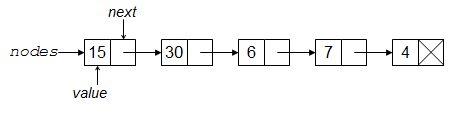
\includegraphics[width=1.0\linewidth,height=6.5in,keepaspectratio]{../images/5.png}
\end{center}
\raggedright{}\myfigurewithoutcaption{5}
\end{minipage}\vspace{0.75cm}


\end{center}


Such chains are more commonly referred to as {\itshape linked-{}lists} \setmainfont[Path=/usr/share/fonts/truetype/cmu/,UprightFont=cmunrm.ttf,BoldFont=cmunbx.ttf,ItalicFont=cmunti.ttf,BoldItalicFont=cmunbi.ttf]{cmunrm.ttf}\setmonofont[Path=/usr/share/fonts/truetype/cmu/,UprightFont=cmuntt.ttf,BoldFont=cmuntb.ttf,ItalicFont=cmunit.ttf,BoldItalicFont=cmuntx.ttf]{cmunrm.ttf}. However, we generally prefer to think in terms of {\itshape lists} \setmainfont[Path=/usr/share/fonts/truetype/cmu/,UprightFont=cmunrm.ttf,BoldFont=cmunbx.ttf,ItalicFont=cmunti.ttf,BoldItalicFont=cmunbi.ttf]{cmunrm.ttf}\setmonofont[Path=/usr/share/fonts/truetype/cmu/,UprightFont=cmuntt.ttf,BoldFont=cmuntb.ttf,ItalicFont=cmunit.ttf,BoldItalicFont=cmuntx.ttf]{cmunrm.ttf} or {\itshape sequences} \setmainfont[Path=/usr/share/fonts/truetype/cmu/,UprightFont=cmunrm.ttf,BoldFont=cmunbx.ttf,ItalicFont=cmunti.ttf,BoldItalicFont=cmunbi.ttf]{cmunrm.ttf}\setmonofont[Path=/usr/share/fonts/truetype/cmu/,UprightFont=cmuntt.ttf,BoldFont=cmuntb.ttf,ItalicFont=cmunit.ttf,BoldItalicFont=cmuntx.ttf]{cmunrm.ttf}, which aren\textquotesingle{}t as low-{}level: the linking concept is just an implementation detail. While a list can be made with a chain, in this book we cover several other ways to make a list. For the moment, we care more about the abstraction capabilities of the node than we do about one of the ways it is used.

The above algorithm only uses the make-{}node, get-{}value, and get-{}next functions. If we use set-{}next we can change the algorithm to generate the chain so that it keeps the original ordering (instead of reversing it).

\LaTeXNullTemplate{}
\\

\TemplateSpaceIndent{$\text{ }${}program$\text{ }${}(input-{}stream$\text{ }${}{\itshape in} \setmainfont[Path=/usr/share/fonts/truetype/cmu/,UprightFont=cmunrm.ttf,BoldFont=cmunbx.ttf,ItalicFont=cmunti.ttf,BoldItalicFont=cmunbi.ttf]{cmunrm.ttf}\setmonofont[Path=/usr/share/fonts/truetype/cmu/,UprightFont=cmuntt.ttf,BoldFont=cmuntb.ttf,ItalicFont=cmunit.ttf,BoldItalicFont=cmuntx.ttf]{cmunrm.ttf},$\text{ }${}output-{}stream$\text{ }${}{\itshape out} \setmainfont[Path=/usr/share/fonts/truetype/cmu/,UprightFont=cmunrm.ttf,BoldFont=cmunbx.ttf,ItalicFont=cmunti.ttf,BoldItalicFont=cmunbi.ttf]{cmunrm.ttf}\setmonofont[Path=/usr/share/fonts/truetype/cmu/,UprightFont=cmuntt.ttf,BoldFont=cmuntb.ttf,ItalicFont=cmunit.ttf,BoldItalicFont=cmuntx.ttf]{cmunrm.ttf})$\text{ }$\newline{}
$\text{ }${}$\text{ }${}$\text{ }${}let$\text{ }${}{\itshape largest} $\text{ }${}\setmainfont[Path=/usr/share/fonts/truetype/cmu/,UprightFont=cmunrm.ttf,BoldFont=cmunbx.ttf,ItalicFont=cmunti.ttf,BoldItalicFont=cmunbi.ttf]{cmunrm.ttf}\setmonofont[Path=/usr/share/fonts/truetype/cmu/,UprightFont=cmuntt.ttf,BoldFont=cmuntb.ttf,ItalicFont=cmunit.ttf,BoldItalicFont=cmuntx.ttf]{cmunrm.ttf}:=$\text{ }${}{$-\infty$}$\text{ }$\newline{}
$\text{ }${}$\text{ }${}$\text{ }${}let$\text{ }${}{\itshape nodes} $\text{ }${}\setmainfont[Path=/usr/share/fonts/truetype/cmu/,UprightFont=cmunrm.ttf,BoldFont=cmunbx.ttf,ItalicFont=cmunti.ttf,BoldItalicFont=cmunbi.ttf]{cmunrm.ttf}\setmonofont[Path=/usr/share/fonts/truetype/cmu/,UprightFont=cmuntt.ttf,BoldFont=cmuntb.ttf,ItalicFont=cmunit.ttf,BoldItalicFont=cmuntx.ttf]{cmunrm.ttf}:=$\text{ }${}null$\text{ }$\newline{}
$\text{ }${}$\text{ }${}$\text{ }${}let$\text{ }${}{\itshape tail\_node} $\text{ }${}\setmainfont[Path=/usr/share/fonts/truetype/cmu/,UprightFont=cmunrm.ttf,BoldFont=cmunbx.ttf,ItalicFont=cmunti.ttf,BoldItalicFont=cmunbi.ttf]{cmunrm.ttf}\setmonofont[Path=/usr/share/fonts/truetype/cmu/,UprightFont=cmuntt.ttf,BoldFont=cmuntb.ttf,ItalicFont=cmunit.ttf,BoldItalicFont=cmuntx.ttf]{cmunrm.ttf}:=$\text{ }${}null$\text{ }$\newline{}
$\text{ }${}$\text{ }${}$\text{ }${}$\text{ }$\newline{}
$\text{ }${}$\text{ }${}$\text{ }${}while$\text{ }${}has-{}next-{}integer$\text{ }${}({\itshape in} \setmainfont[Path=/usr/share/fonts/truetype/cmu/,UprightFont=cmunrm.ttf,BoldFont=cmunbx.ttf,ItalicFont=cmunti.ttf,BoldItalicFont=cmunbi.ttf]{cmunrm.ttf}\setmonofont[Path=/usr/share/fonts/truetype/cmu/,UprightFont=cmuntt.ttf,BoldFont=cmuntb.ttf,ItalicFont=cmunit.ttf,BoldItalicFont=cmuntx.ttf]{cmunrm.ttf}):$\text{ }$\newline{}
$\text{ }${}$\text{ }${}$\text{ }${}$\text{ }${}$\text{ }${}let$\text{ }${}{\itshape i} $\text{ }${}\setmainfont[Path=/usr/share/fonts/truetype/cmu/,UprightFont=cmunrm.ttf,BoldFont=cmunbx.ttf,ItalicFont=cmunti.ttf,BoldItalicFont=cmunbi.ttf]{cmunrm.ttf}\setmonofont[Path=/usr/share/fonts/truetype/cmu/,UprightFont=cmuntt.ttf,BoldFont=cmuntb.ttf,ItalicFont=cmunit.ttf,BoldItalicFont=cmuntx.ttf]{cmunrm.ttf}:=$\text{ }${}read-{}integer$\text{ }${}({\itshape in} \setmainfont[Path=/usr/share/fonts/truetype/cmu/,UprightFont=cmunrm.ttf,BoldFont=cmunbx.ttf,ItalicFont=cmunti.ttf,BoldItalicFont=cmunbi.ttf]{cmunrm.ttf}\setmonofont[Path=/usr/share/fonts/truetype/cmu/,UprightFont=cmuntt.ttf,BoldFont=cmuntb.ttf,ItalicFont=cmunit.ttf,BoldItalicFont=cmuntx.ttf]{cmunrm.ttf})$\text{ }$\newline{}
$\text{ }${}$\text{ }${}$\text{ }${}$\text{ }${}$\text{ }${}if$\text{ }${}({\itshape nodes} $\text{ }${}\setmainfont[Path=/usr/share/fonts/truetype/cmu/,UprightFont=cmunrm.ttf,BoldFont=cmunbx.ttf,ItalicFont=cmunti.ttf,BoldItalicFont=cmunbi.ttf]{cmunrm.ttf}\setmonofont[Path=/usr/share/fonts/truetype/cmu/,UprightFont=cmuntt.ttf,BoldFont=cmuntb.ttf,ItalicFont=cmunit.ttf,BoldItalicFont=cmuntx.ttf]{cmunrm.ttf}==$\text{ }${}null)$\text{ }$\newline{}
$\text{ }${}$\text{ }${}$\text{ }${}$\text{ }${}$\text{ }${}$\text{ }${}$\text{ }${}{\itshape nodes} $\text{ }${}\setmainfont[Path=/usr/share/fonts/truetype/cmu/,UprightFont=cmunrm.ttf,BoldFont=cmunbx.ttf,ItalicFont=cmunti.ttf,BoldItalicFont=cmunbi.ttf]{cmunrm.ttf}\setmonofont[Path=/usr/share/fonts/truetype/cmu/,UprightFont=cmuntt.ttf,BoldFont=cmuntb.ttf,ItalicFont=cmunit.ttf,BoldItalicFont=cmuntx.ttf]{cmunrm.ttf}:=$\text{ }${}{\bfseries \setmainfont[Path=/usr/share/fonts/truetype/cmu/,UprightFont=cmunrm.ttf,BoldFont=cmunbx.ttf,ItalicFont=cmunti.ttf,BoldItalicFont=cmunbi.ttf]{cmunbx.ttf}\setmonofont[Path=/usr/share/fonts/truetype/cmu/,UprightFont=cmuntt.ttf,BoldFont=cmuntb.ttf,ItalicFont=cmunit.ttf,BoldItalicFont=cmuntx.ttf]{cmunbx.ttf}\bfseries make-{}node} \setmainfont[Path=/usr/share/fonts/truetype/cmu/,UprightFont=cmunrm.ttf,BoldFont=cmunbx.ttf,ItalicFont=cmunti.ttf,BoldItalicFont=cmunbi.ttf]{cmunrm.ttf}\setmonofont[Path=/usr/share/fonts/truetype/cmu/,UprightFont=cmuntt.ttf,BoldFont=cmuntb.ttf,ItalicFont=cmunit.ttf,BoldItalicFont=cmuntx.ttf]{cmunrm.ttf}({\itshape i} \setmainfont[Path=/usr/share/fonts/truetype/cmu/,UprightFont=cmunrm.ttf,BoldFont=cmunbx.ttf,ItalicFont=cmunti.ttf,BoldItalicFont=cmunbi.ttf]{cmunrm.ttf}\setmonofont[Path=/usr/share/fonts/truetype/cmu/,UprightFont=cmuntt.ttf,BoldFont=cmuntb.ttf,ItalicFont=cmunit.ttf,BoldItalicFont=cmuntx.ttf]{cmunrm.ttf},$\text{ }${}null)$\text{ }${}{\itshape // construct first node in the list} $\text{ }$\newline{}
$\text{ }${}$\text{ }${}$\text{ }${}$\text{ }${}$\text{ }${}$\text{ }${}$\text{ }${}{\itshape tail\_node} $\text{ }${}\setmainfont[Path=/usr/share/fonts/truetype/cmu/,UprightFont=cmunrm.ttf,BoldFont=cmunbx.ttf,ItalicFont=cmunti.ttf,BoldItalicFont=cmunbi.ttf]{cmunrm.ttf}\setmonofont[Path=/usr/share/fonts/truetype/cmu/,UprightFont=cmuntt.ttf,BoldFont=cmuntb.ttf,ItalicFont=cmunit.ttf,BoldItalicFont=cmuntx.ttf]{cmunrm.ttf}:=$\text{ }${}{\itshape nodes} $\text{ }${}{\itshape //there is one node in the list=>{} first and last are the same} $\text{ }$\newline{}
$\text{ }${}$\text{ }${}$\text{ }${}$\text{ }${}$\text{ }${}\setmainfont[Path=/usr/share/fonts/truetype/cmu/,UprightFont=cmunrm.ttf,BoldFont=cmunbx.ttf,ItalicFont=cmunti.ttf,BoldItalicFont=cmunbi.ttf]{cmunrm.ttf}\setmonofont[Path=/usr/share/fonts/truetype/cmu/,UprightFont=cmuntt.ttf,BoldFont=cmuntb.ttf,ItalicFont=cmunit.ttf,BoldItalicFont=cmuntx.ttf]{cmunrm.ttf}else$\text{ }$\newline{}
$\text{ }${}$\text{ }${}$\text{ }${}$\text{ }${}$\text{ }${}$\text{ }${}$\text{ }${}{\itshape tail\_node} $\text{ }${}\setmainfont[Path=/usr/share/fonts/truetype/cmu/,UprightFont=cmunrm.ttf,BoldFont=cmunbx.ttf,ItalicFont=cmunti.ttf,BoldItalicFont=cmunbi.ttf]{cmunrm.ttf}\setmonofont[Path=/usr/share/fonts/truetype/cmu/,UprightFont=cmuntt.ttf,BoldFont=cmuntb.ttf,ItalicFont=cmunit.ttf,BoldItalicFont=cmuntx.ttf]{cmunrm.ttf}:=$\text{ }${}{\bfseries \setmainfont[Path=/usr/share/fonts/truetype/cmu/,UprightFont=cmunrm.ttf,BoldFont=cmunbx.ttf,ItalicFont=cmunti.ttf,BoldItalicFont=cmunbi.ttf]{cmunbx.ttf}\setmonofont[Path=/usr/share/fonts/truetype/cmu/,UprightFont=cmuntt.ttf,BoldFont=cmuntb.ttf,ItalicFont=cmunit.ttf,BoldItalicFont=cmuntx.ttf]{cmunbx.ttf}\bfseries set-{}next} $\text{ }${}\setmainfont[Path=/usr/share/fonts/truetype/cmu/,UprightFont=cmunrm.ttf,BoldFont=cmunbx.ttf,ItalicFont=cmunti.ttf,BoldItalicFont=cmunbi.ttf]{cmunrm.ttf}\setmonofont[Path=/usr/share/fonts/truetype/cmu/,UprightFont=cmuntt.ttf,BoldFont=cmuntb.ttf,ItalicFont=cmunit.ttf,BoldItalicFont=cmuntx.ttf]{cmunrm.ttf}({\itshape tail\_node} \setmainfont[Path=/usr/share/fonts/truetype/cmu/,UprightFont=cmunrm.ttf,BoldFont=cmunbx.ttf,ItalicFont=cmunti.ttf,BoldItalicFont=cmunbi.ttf]{cmunrm.ttf}\setmonofont[Path=/usr/share/fonts/truetype/cmu/,UprightFont=cmuntt.ttf,BoldFont=cmuntb.ttf,ItalicFont=cmunit.ttf,BoldItalicFont=cmuntx.ttf]{cmunrm.ttf},$\text{ }${}{\bfseries \setmainfont[Path=/usr/share/fonts/truetype/cmu/,UprightFont=cmunrm.ttf,BoldFont=cmunbx.ttf,ItalicFont=cmunti.ttf,BoldItalicFont=cmunbi.ttf]{cmunbx.ttf}\setmonofont[Path=/usr/share/fonts/truetype/cmu/,UprightFont=cmuntt.ttf,BoldFont=cmuntb.ttf,ItalicFont=cmunit.ttf,BoldItalicFont=cmuntx.ttf]{cmunbx.ttf}\bfseries make-{}node} $\text{ }${}\setmainfont[Path=/usr/share/fonts/truetype/cmu/,UprightFont=cmunrm.ttf,BoldFont=cmunbx.ttf,ItalicFont=cmunti.ttf,BoldItalicFont=cmunbi.ttf]{cmunrm.ttf}\setmonofont[Path=/usr/share/fonts/truetype/cmu/,UprightFont=cmuntt.ttf,BoldFont=cmuntb.ttf,ItalicFont=cmunit.ttf,BoldItalicFont=cmuntx.ttf]{cmunrm.ttf}({\itshape i} \setmainfont[Path=/usr/share/fonts/truetype/cmu/,UprightFont=cmunrm.ttf,BoldFont=cmunbx.ttf,ItalicFont=cmunti.ttf,BoldItalicFont=cmunbi.ttf]{cmunrm.ttf}\setmonofont[Path=/usr/share/fonts/truetype/cmu/,UprightFont=cmuntt.ttf,BoldFont=cmuntb.ttf,ItalicFont=cmunit.ttf,BoldItalicFont=cmuntx.ttf]{cmunrm.ttf},$\text{ }${}null))$\text{ }${}{\itshape // append new node to the end of the list} $\text{ }$\newline{}
$\text{ }${}$\text{ }${}$\text{ }${}$\text{ }${}$\text{ }${}{\itshape largest} $\text{ }${}\setmainfont[Path=/usr/share/fonts/truetype/cmu/,UprightFont=cmunrm.ttf,BoldFont=cmunbx.ttf,ItalicFont=cmunti.ttf,BoldItalicFont=cmunbi.ttf]{cmunrm.ttf}\setmonofont[Path=/usr/share/fonts/truetype/cmu/,UprightFont=cmuntt.ttf,BoldFont=cmuntb.ttf,ItalicFont=cmunit.ttf,BoldItalicFont=cmuntx.ttf]{cmunrm.ttf}:=$\text{ }${}max({\itshape largest} \setmainfont[Path=/usr/share/fonts/truetype/cmu/,UprightFont=cmunrm.ttf,BoldFont=cmunbx.ttf,ItalicFont=cmunti.ttf,BoldItalicFont=cmunbi.ttf]{cmunrm.ttf}\setmonofont[Path=/usr/share/fonts/truetype/cmu/,UprightFont=cmuntt.ttf,BoldFont=cmuntb.ttf,ItalicFont=cmunit.ttf,BoldItalicFont=cmuntx.ttf]{cmunrm.ttf},$\text{ }${}{\itshape i} \setmainfont[Path=/usr/share/fonts/truetype/cmu/,UprightFont=cmunrm.ttf,BoldFont=cmunbx.ttf,ItalicFont=cmunti.ttf,BoldItalicFont=cmunbi.ttf]{cmunrm.ttf}\setmonofont[Path=/usr/share/fonts/truetype/cmu/,UprightFont=cmuntt.ttf,BoldFont=cmuntb.ttf,ItalicFont=cmunit.ttf,BoldItalicFont=cmuntx.ttf]{cmunrm.ttf})$\text{ }$\newline{}
$\text{ }${}$\text{ }${}$\text{ }${}repeat$\text{ }$\newline{}
$\text{ }${}$\text{ }${}$\text{ }${}println$\text{ }${}{\itshape out} $\text{ }${}\setmainfont[Path=/usr/share/fonts/truetype/cmu/,UprightFont=cmunrm.ttf,BoldFont=cmunbx.ttf,ItalicFont=cmunti.ttf,BoldItalicFont=cmunbi.ttf]{cmunrm.ttf}\setmonofont[Path=/usr/share/fonts/truetype/cmu/,UprightFont=cmuntt.ttf,BoldFont=cmuntb.ttf,ItalicFont=cmunit.ttf,BoldItalicFont=cmuntx.ttf]{cmunrm.ttf}\symbol{34}Maximum:$\text{ }${}\symbol{34}$\text{ }${}{\itshape largest} $\text{ }$\newline{}
$\text{ }${}$\text{ }$\newline{}
$\text{ }${}$\text{ }${}$\text{ }${}{\itshape // now compute the averages of all factors of largest} $\text{ }$\newline{}
$\text{ }${}$\text{ }${}$\text{ }${}\setmainfont[Path=/usr/share/fonts/truetype/cmu/,UprightFont=cmunrm.ttf,BoldFont=cmunbx.ttf,ItalicFont=cmunti.ttf,BoldItalicFont=cmunbi.ttf]{cmunrm.ttf}\setmonofont[Path=/usr/share/fonts/truetype/cmu/,UprightFont=cmuntt.ttf,BoldFont=cmuntb.ttf,ItalicFont=cmunit.ttf,BoldItalicFont=cmuntx.ttf]{cmunrm.ttf}let$\text{ }${}{\itshape total} $\text{ }${}\setmainfont[Path=/usr/share/fonts/truetype/cmu/,UprightFont=cmunrm.ttf,BoldFont=cmunbx.ttf,ItalicFont=cmunti.ttf,BoldItalicFont=cmunbi.ttf]{cmunrm.ttf}\setmonofont[Path=/usr/share/fonts/truetype/cmu/,UprightFont=cmuntt.ttf,BoldFont=cmuntb.ttf,ItalicFont=cmunit.ttf,BoldItalicFont=cmuntx.ttf]{cmunrm.ttf}:=$\text{ }${}0$\text{ }$\newline{}
$\text{ }${}$\text{ }${}$\text{ }${}let$\text{ }${}{\itshape count} $\text{ }${}\setmainfont[Path=/usr/share/fonts/truetype/cmu/,UprightFont=cmunrm.ttf,BoldFont=cmunbx.ttf,ItalicFont=cmunti.ttf,BoldItalicFont=cmunbi.ttf]{cmunrm.ttf}\setmonofont[Path=/usr/share/fonts/truetype/cmu/,UprightFont=cmuntt.ttf,BoldFont=cmuntb.ttf,ItalicFont=cmunit.ttf,BoldItalicFont=cmuntx.ttf]{cmunrm.ttf}:=$\text{ }${}0$\text{ }$\newline{}
$\text{ }${}$\text{ }${}$\text{ }${}while$\text{ }${}{\itshape nodes} $\text{ }${}\setmainfont[Path=/usr/share/fonts/truetype/cmu/,UprightFont=cmunrm.ttf,BoldFont=cmunbx.ttf,ItalicFont=cmunti.ttf,BoldItalicFont=cmunbi.ttf]{cmunrm.ttf}\setmonofont[Path=/usr/share/fonts/truetype/cmu/,UprightFont=cmuntt.ttf,BoldFont=cmuntb.ttf,ItalicFont=cmunit.ttf,BoldItalicFont=cmuntx.ttf]{cmunrm.ttf}!=$\text{ }${}null:$\text{ }$\newline{}
$\text{ }${}$\text{ }${}$\text{ }${}$\text{ }${}$\text{ }${}let$\text{ }${}{\itshape j} $\text{ }${}\setmainfont[Path=/usr/share/fonts/truetype/cmu/,UprightFont=cmunrm.ttf,BoldFont=cmunbx.ttf,ItalicFont=cmunti.ttf,BoldItalicFont=cmunbi.ttf]{cmunrm.ttf}\setmonofont[Path=/usr/share/fonts/truetype/cmu/,UprightFont=cmuntt.ttf,BoldFont=cmuntb.ttf,ItalicFont=cmunit.ttf,BoldItalicFont=cmuntx.ttf]{cmunrm.ttf}:=$\text{ }${}{\bfseries \setmainfont[Path=/usr/share/fonts/truetype/cmu/,UprightFont=cmunrm.ttf,BoldFont=cmunbx.ttf,ItalicFont=cmunti.ttf,BoldItalicFont=cmunbi.ttf]{cmunbx.ttf}\setmonofont[Path=/usr/share/fonts/truetype/cmu/,UprightFont=cmuntt.ttf,BoldFont=cmuntb.ttf,ItalicFont=cmunit.ttf,BoldItalicFont=cmuntx.ttf]{cmunbx.ttf}\bfseries get-{}value} \setmainfont[Path=/usr/share/fonts/truetype/cmu/,UprightFont=cmunrm.ttf,BoldFont=cmunbx.ttf,ItalicFont=cmunti.ttf,BoldItalicFont=cmunbi.ttf]{cmunrm.ttf}\setmonofont[Path=/usr/share/fonts/truetype/cmu/,UprightFont=cmuntt.ttf,BoldFont=cmuntb.ttf,ItalicFont=cmunit.ttf,BoldItalicFont=cmuntx.ttf]{cmunrm.ttf}({\itshape nodes} \setmainfont[Path=/usr/share/fonts/truetype/cmu/,UprightFont=cmunrm.ttf,BoldFont=cmunbx.ttf,ItalicFont=cmunti.ttf,BoldItalicFont=cmunbi.ttf]{cmunrm.ttf}\setmonofont[Path=/usr/share/fonts/truetype/cmu/,UprightFont=cmuntt.ttf,BoldFont=cmuntb.ttf,ItalicFont=cmunit.ttf,BoldItalicFont=cmuntx.ttf]{cmunrm.ttf})$\text{ }$\newline{}
$\text{ }${}$\text{ }${}$\text{ }${}$\text{ }${}$\text{ }${}if$\text{ }${}{\itshape j} $\text{ }${}\setmainfont[Path=/usr/share/fonts/truetype/cmu/,UprightFont=cmunrm.ttf,BoldFont=cmunbx.ttf,ItalicFont=cmunti.ttf,BoldItalicFont=cmunbi.ttf]{cmunrm.ttf}\setmonofont[Path=/usr/share/fonts/truetype/cmu/,UprightFont=cmuntt.ttf,BoldFont=cmuntb.ttf,ItalicFont=cmunit.ttf,BoldItalicFont=cmuntx.ttf]{cmunrm.ttf}divides$\text{ }${}{\itshape largest} \setmainfont[Path=/usr/share/fonts/truetype/cmu/,UprightFont=cmunrm.ttf,BoldFont=cmunbx.ttf,ItalicFont=cmunti.ttf,BoldItalicFont=cmunbi.ttf]{cmunrm.ttf}\setmonofont[Path=/usr/share/fonts/truetype/cmu/,UprightFont=cmuntt.ttf,BoldFont=cmuntb.ttf,ItalicFont=cmunit.ttf,BoldItalicFont=cmuntx.ttf]{cmunrm.ttf}:$\text{ }$\newline{}
$\text{ }${}$\text{ }${}$\text{ }${}$\text{ }${}$\text{ }${}$\text{ }${}$\text{ }${}{\itshape total} $\text{ }${}\setmainfont[Path=/usr/share/fonts/truetype/cmu/,UprightFont=cmunrm.ttf,BoldFont=cmunbx.ttf,ItalicFont=cmunti.ttf,BoldItalicFont=cmunbi.ttf]{cmunrm.ttf}\setmonofont[Path=/usr/share/fonts/truetype/cmu/,UprightFont=cmuntt.ttf,BoldFont=cmuntb.ttf,ItalicFont=cmunit.ttf,BoldItalicFont=cmuntx.ttf]{cmunrm.ttf}:=$\text{ }${}{\itshape total} $\text{ }${}\setmainfont[Path=/usr/share/fonts/truetype/cmu/,UprightFont=cmunrm.ttf,BoldFont=cmunbx.ttf,ItalicFont=cmunti.ttf,BoldItalicFont=cmunbi.ttf]{cmunrm.ttf}\setmonofont[Path=/usr/share/fonts/truetype/cmu/,UprightFont=cmuntt.ttf,BoldFont=cmuntb.ttf,ItalicFont=cmunit.ttf,BoldItalicFont=cmuntx.ttf]{cmunrm.ttf}+$\text{ }${}{\itshape j} $\text{ }$\newline{}
$\text{ }${}$\text{ }${}$\text{ }${}$\text{ }${}$\text{ }${}$\text{ }${}$\text{ }${}{\itshape count} $\text{ }${}\setmainfont[Path=/usr/share/fonts/truetype/cmu/,UprightFont=cmunrm.ttf,BoldFont=cmunbx.ttf,ItalicFont=cmunti.ttf,BoldItalicFont=cmunbi.ttf]{cmunrm.ttf}\setmonofont[Path=/usr/share/fonts/truetype/cmu/,UprightFont=cmuntt.ttf,BoldFont=cmuntb.ttf,ItalicFont=cmunit.ttf,BoldItalicFont=cmuntx.ttf]{cmunrm.ttf}:=$\text{ }${}{\itshape count} $\text{ }${}\setmainfont[Path=/usr/share/fonts/truetype/cmu/,UprightFont=cmunrm.ttf,BoldFont=cmunbx.ttf,ItalicFont=cmunti.ttf,BoldItalicFont=cmunbi.ttf]{cmunrm.ttf}\setmonofont[Path=/usr/share/fonts/truetype/cmu/,UprightFont=cmuntt.ttf,BoldFont=cmuntb.ttf,ItalicFont=cmunit.ttf,BoldItalicFont=cmuntx.ttf]{cmunrm.ttf}+$\text{ }${}1$\text{ }$\newline{}
$\text{ }${}$\text{ }${}$\text{ }${}$\text{ }${}$\text{ }${}fi$\text{ }$\newline{}
$\text{ }${}$\text{ }${}$\text{ }${}$\text{ }${}$\text{ }${}{\itshape nodes} $\text{ }${}\setmainfont[Path=/usr/share/fonts/truetype/cmu/,UprightFont=cmunrm.ttf,BoldFont=cmunbx.ttf,ItalicFont=cmunti.ttf,BoldItalicFont=cmunbi.ttf]{cmunrm.ttf}\setmonofont[Path=/usr/share/fonts/truetype/cmu/,UprightFont=cmuntt.ttf,BoldFont=cmuntb.ttf,ItalicFont=cmunit.ttf,BoldItalicFont=cmuntx.ttf]{cmunrm.ttf}:=$\text{ }${}{\bfseries \setmainfont[Path=/usr/share/fonts/truetype/cmu/,UprightFont=cmunrm.ttf,BoldFont=cmunbx.ttf,ItalicFont=cmunti.ttf,BoldItalicFont=cmunbi.ttf]{cmunbx.ttf}\setmonofont[Path=/usr/share/fonts/truetype/cmu/,UprightFont=cmuntt.ttf,BoldFont=cmuntb.ttf,ItalicFont=cmunit.ttf,BoldItalicFont=cmuntx.ttf]{cmunbx.ttf}\bfseries get-{}next} \setmainfont[Path=/usr/share/fonts/truetype/cmu/,UprightFont=cmunrm.ttf,BoldFont=cmunbx.ttf,ItalicFont=cmunti.ttf,BoldItalicFont=cmunbi.ttf]{cmunrm.ttf}\setmonofont[Path=/usr/share/fonts/truetype/cmu/,UprightFont=cmuntt.ttf,BoldFont=cmuntb.ttf,ItalicFont=cmunit.ttf,BoldItalicFont=cmuntx.ttf]{cmunrm.ttf}({\itshape nodes} \setmainfont[Path=/usr/share/fonts/truetype/cmu/,UprightFont=cmunrm.ttf,BoldFont=cmunbx.ttf,ItalicFont=cmunti.ttf,BoldItalicFont=cmunbi.ttf]{cmunrm.ttf}\setmonofont[Path=/usr/share/fonts/truetype/cmu/,UprightFont=cmuntt.ttf,BoldFont=cmuntb.ttf,ItalicFont=cmunit.ttf,BoldItalicFont=cmuntx.ttf]{cmunrm.ttf})$\text{ }$\newline{}
$\text{ }${}$\text{ }${}$\text{ }${}repeat$\text{ }$\newline{}
$\text{ }${}$\text{ }${}$\text{ }${}if$\text{ }${}{\itshape count} $\text{ }${}\setmainfont[Path=/usr/share/fonts/truetype/cmu/,UprightFont=cmunrm.ttf,BoldFont=cmunbx.ttf,ItalicFont=cmunti.ttf,BoldItalicFont=cmunbi.ttf]{cmunrm.ttf}\setmonofont[Path=/usr/share/fonts/truetype/cmu/,UprightFont=cmuntt.ttf,BoldFont=cmuntb.ttf,ItalicFont=cmunit.ttf,BoldItalicFont=cmuntx.ttf]{cmunrm.ttf}!=$\text{ }${}0:$\text{ }$\newline{}
$\text{ }${}$\text{ }${}$\text{ }${}$\text{ }${}$\text{ }${}println$\text{ }${}{\itshape out} $\text{ }${}\setmainfont[Path=/usr/share/fonts/truetype/cmu/,UprightFont=cmunrm.ttf,BoldFont=cmunbx.ttf,ItalicFont=cmunti.ttf,BoldItalicFont=cmunbi.ttf]{cmunrm.ttf}\setmonofont[Path=/usr/share/fonts/truetype/cmu/,UprightFont=cmuntt.ttf,BoldFont=cmuntb.ttf,ItalicFont=cmunit.ttf,BoldItalicFont=cmuntx.ttf]{cmunrm.ttf}\symbol{34}Average:$\text{ }${}\symbol{34}$\text{ }${}({\itshape total} $\text{ }${}\setmainfont[Path=/usr/share/fonts/truetype/cmu/,UprightFont=cmunrm.ttf,BoldFont=cmunbx.ttf,ItalicFont=cmunti.ttf,BoldItalicFont=cmunbi.ttf]{cmunrm.ttf}\setmonofont[Path=/usr/share/fonts/truetype/cmu/,UprightFont=cmuntt.ttf,BoldFont=cmuntb.ttf,ItalicFont=cmunit.ttf,BoldItalicFont=cmuntx.ttf]{cmunrm.ttf}/$\text{ }${}{\itshape count} \setmainfont[Path=/usr/share/fonts/truetype/cmu/,UprightFont=cmunrm.ttf,BoldFont=cmunbx.ttf,ItalicFont=cmunti.ttf,BoldItalicFont=cmunbi.ttf]{cmunrm.ttf}\setmonofont[Path=/usr/share/fonts/truetype/cmu/,UprightFont=cmuntt.ttf,BoldFont=cmuntb.ttf,ItalicFont=cmunit.ttf,BoldItalicFont=cmuntx.ttf]{cmunrm.ttf})$\text{ }$\newline{}
$\text{ }${}$\text{ }${}$\text{ }${}fi$\text{ }$\newline{}
$\text{ }${}end}

\subsection{The Principle of Induction}
\label{4}
The chains we can build from nodes are a demonstration of the principle of mathematical induction:


\begin{longtable}{>{\RaggedRight}p{0.97143\linewidth}} 
\hspace*{0pt}\ignorespaces{}\hspace*{0pt}{\bfseries \setmainfont[Path=/usr/share/fonts/truetype/cmu/,UprightFont=cmunrm.ttf,BoldFont=cmunbx.ttf,ItalicFont=cmunti.ttf,BoldItalicFont=cmunbi.ttf]{cmunbx.ttf}\setmonofont[Path=/usr/share/fonts/truetype/cmu/,UprightFont=cmuntt.ttf,BoldFont=cmuntb.ttf,ItalicFont=cmunit.ttf,BoldItalicFont=cmuntx.ttf]{cmunbx.ttf}\bfseries Mathematical Induction} \newline{}\setmainfont[Path=/usr/share/fonts/truetype/cmu/,UprightFont=cmunrm.ttf,BoldFont=cmunbx.ttf,ItalicFont=cmunti.ttf,BoldItalicFont=cmunbi.ttf]{cmunrm.ttf}\setmonofont[Path=/usr/share/fonts/truetype/cmu/,UprightFont=cmuntt.ttf,BoldFont=cmuntb.ttf,ItalicFont=cmunit.ttf,BoldItalicFont=cmuntx.ttf]{cmunrm.ttf}\# Suppose you have some property of numbers {$P(n)$}\# If you can prove that when {$P(n)$} holds that {$P(n+1)$} must also hold, then\# All you need to do is prove that {$P(1)$} holds to show that {$P(n)$} holds for all natural {$n$} 
\end{longtable}


For example, let the property {$P(n)$} be the statement that \symbol{34}you can make a chain that holds {$n$} numbers\symbol{34}. This is a property of natural numbers, because the sentence makes sense for specific values of {$n$}:

\begin{myitemize}
\item{}  you can make a chain that holds 5 numbers
\item{}  you can make a chain that holds 100 numbers
\item{}  you can make a chain that holds 1,000,000 numbers
\end{myitemize}


Instead of proving that we can make chains of length 5, 100, and one million, we\textquotesingle{}d rather prove the general statement {$P(n)$} instead. Step 2 above is called the {\bfseries \setmainfont[Path=/usr/share/fonts/truetype/cmu/,UprightFont=cmunrm.ttf,BoldFont=cmunbx.ttf,ItalicFont=cmunti.ttf,BoldItalicFont=cmunbi.ttf]{cmunbx.ttf}\setmonofont[Path=/usr/share/fonts/truetype/cmu/,UprightFont=cmuntt.ttf,BoldFont=cmuntb.ttf,ItalicFont=cmunit.ttf,BoldItalicFont=cmuntx.ttf]{cmunbx.ttf}\bfseries Inductive Hypothesis} \setmainfont[Path=/usr/share/fonts/truetype/cmu/,UprightFont=cmunrm.ttf,BoldFont=cmunbx.ttf,ItalicFont=cmunti.ttf,BoldItalicFont=cmunbi.ttf]{cmunrm.ttf}\setmonofont[Path=/usr/share/fonts/truetype/cmu/,UprightFont=cmuntt.ttf,BoldFont=cmuntb.ttf,ItalicFont=cmunit.ttf,BoldItalicFont=cmuntx.ttf]{cmunrm.ttf}; let\textquotesingle{}s show that we can prove it:

\begin{myitemize}
\item{}  Assume that {$P(n)$} holds. That is, that we can make a chain of {$n$} elements. Now we must show that {$P(n+1)$} holds.
\item{}  Assume {\ttfamily {\ttfamily \itshape chain}} \setmainfont[Path=/usr/share/fonts/truetype/cmu/,UprightFont=cmunrm.ttf,BoldFont=cmunbx.ttf,ItalicFont=cmunti.ttf,BoldItalicFont=cmunbi.ttf]{cmunrm.ttf}\setmonofont[Path=/usr/share/fonts/truetype/cmu/,UprightFont=cmuntt.ttf,BoldFont=cmuntb.ttf,ItalicFont=cmunit.ttf,BoldItalicFont=cmuntx.ttf]{cmunrm.ttf} is the first node of the {$n$}-{}element chain. Assume {\ttfamily {\ttfamily \itshape i}} \setmainfont[Path=/usr/share/fonts/truetype/cmu/,UprightFont=cmunrm.ttf,BoldFont=cmunbx.ttf,ItalicFont=cmunti.ttf,BoldItalicFont=cmunbi.ttf]{cmunrm.ttf}\setmonofont[Path=/usr/share/fonts/truetype/cmu/,UprightFont=cmuntt.ttf,BoldFont=cmuntb.ttf,ItalicFont=cmunit.ttf,BoldItalicFont=cmuntx.ttf]{cmunrm.ttf} is some number that we\textquotesingle{}d like to add to the chain to make an {$n+1$} length chain.
\item{}  The following code can accomplish this for us:
\end{myitemize}
\\

\TemplateSpaceIndent{$\text{ }${}let$\text{ }${}{\itshape bigger-{}chain} $\text{ }${}\setmainfont[Path=/usr/share/fonts/truetype/cmu/,UprightFont=cmunrm.ttf,BoldFont=cmunbx.ttf,ItalicFont=cmunti.ttf,BoldItalicFont=cmunbi.ttf]{cmunrm.ttf}\setmonofont[Path=/usr/share/fonts/truetype/cmu/,UprightFont=cmuntt.ttf,BoldFont=cmuntb.ttf,ItalicFont=cmunit.ttf,BoldItalicFont=cmuntx.ttf]{cmunrm.ttf}:=$\text{ }${}{\bfseries \setmainfont[Path=/usr/share/fonts/truetype/cmu/,UprightFont=cmunrm.ttf,BoldFont=cmunbx.ttf,ItalicFont=cmunti.ttf,BoldItalicFont=cmunbi.ttf]{cmunbx.ttf}\setmonofont[Path=/usr/share/fonts/truetype/cmu/,UprightFont=cmuntt.ttf,BoldFont=cmuntb.ttf,ItalicFont=cmunit.ttf,BoldItalicFont=cmuntx.ttf]{cmunbx.ttf}\bfseries make-{}node} \setmainfont[Path=/usr/share/fonts/truetype/cmu/,UprightFont=cmunrm.ttf,BoldFont=cmunbx.ttf,ItalicFont=cmunti.ttf,BoldItalicFont=cmunbi.ttf]{cmunrm.ttf}\setmonofont[Path=/usr/share/fonts/truetype/cmu/,UprightFont=cmuntt.ttf,BoldFont=cmuntb.ttf,ItalicFont=cmunit.ttf,BoldItalicFont=cmuntx.ttf]{cmunrm.ttf}({\itshape i} \setmainfont[Path=/usr/share/fonts/truetype/cmu/,UprightFont=cmunrm.ttf,BoldFont=cmunbx.ttf,ItalicFont=cmunti.ttf,BoldItalicFont=cmunbi.ttf]{cmunrm.ttf}\setmonofont[Path=/usr/share/fonts/truetype/cmu/,UprightFont=cmuntt.ttf,BoldFont=cmuntb.ttf,ItalicFont=cmunit.ttf,BoldItalicFont=cmuntx.ttf]{cmunrm.ttf},$\text{ }${}{\itshape chain} \setmainfont[Path=/usr/share/fonts/truetype/cmu/,UprightFont=cmunrm.ttf,BoldFont=cmunbx.ttf,ItalicFont=cmunti.ttf,BoldItalicFont=cmunbi.ttf]{cmunrm.ttf}\setmonofont[Path=/usr/share/fonts/truetype/cmu/,UprightFont=cmuntt.ttf,BoldFont=cmuntb.ttf,ItalicFont=cmunit.ttf,BoldItalicFont=cmuntx.ttf]{cmunrm.ttf})}

\begin{myitemize}
\item{}  Here, we have the new number {\ttfamily {\ttfamily \itshape i}} \setmainfont[Path=/usr/share/fonts/truetype/cmu/,UprightFont=cmunrm.ttf,BoldFont=cmunbx.ttf,ItalicFont=cmunti.ttf,BoldItalicFont=cmunbi.ttf]{cmunrm.ttf}\setmonofont[Path=/usr/share/fonts/truetype/cmu/,UprightFont=cmuntt.ttf,BoldFont=cmuntb.ttf,ItalicFont=cmunit.ttf,BoldItalicFont=cmuntx.ttf]{cmunrm.ttf} that is now the contained value of the first link of the {\ttfamily {\ttfamily \itshape bigger-{}chain}} \setmainfont[Path=/usr/share/fonts/truetype/cmu/,UprightFont=cmunrm.ttf,BoldFont=cmunbx.ttf,ItalicFont=cmunti.ttf,BoldItalicFont=cmunbi.ttf]{cmunrm.ttf}\setmonofont[Path=/usr/share/fonts/truetype/cmu/,UprightFont=cmuntt.ttf,BoldFont=cmuntb.ttf,ItalicFont=cmunit.ttf,BoldItalicFont=cmuntx.ttf]{cmunrm.ttf}. If {\ttfamily {\ttfamily \itshape chain}} \setmainfont[Path=/usr/share/fonts/truetype/cmu/,UprightFont=cmunrm.ttf,BoldFont=cmunbx.ttf,ItalicFont=cmunti.ttf,BoldItalicFont=cmunbi.ttf]{cmunrm.ttf}\setmonofont[Path=/usr/share/fonts/truetype/cmu/,UprightFont=cmuntt.ttf,BoldFont=cmuntb.ttf,ItalicFont=cmunit.ttf,BoldItalicFont=cmuntx.ttf]{cmunrm.ttf} had {$n$} elements, then {\ttfamily {\ttfamily \itshape bigger-{}chain}} \setmainfont[Path=/usr/share/fonts/truetype/cmu/,UprightFont=cmunrm.ttf,BoldFont=cmunbx.ttf,ItalicFont=cmunti.ttf,BoldItalicFont=cmunbi.ttf]{cmunrm.ttf}\setmonofont[Path=/usr/share/fonts/truetype/cmu/,UprightFont=cmuntt.ttf,BoldFont=cmuntb.ttf,ItalicFont=cmunit.ttf,BoldItalicFont=cmuntx.ttf]{cmunrm.ttf} must have {$n+1$} elements.
\end{myitemize}


Step 3 above is called the {\bfseries \setmainfont[Path=/usr/share/fonts/truetype/cmu/,UprightFont=cmunrm.ttf,BoldFont=cmunbx.ttf,ItalicFont=cmunti.ttf,BoldItalicFont=cmunbi.ttf]{cmunbx.ttf}\setmonofont[Path=/usr/share/fonts/truetype/cmu/,UprightFont=cmuntt.ttf,BoldFont=cmuntb.ttf,ItalicFont=cmunit.ttf,BoldItalicFont=cmuntx.ttf]{cmunbx.ttf}\bfseries Base Case} \setmainfont[Path=/usr/share/fonts/truetype/cmu/,UprightFont=cmunrm.ttf,BoldFont=cmunbx.ttf,ItalicFont=cmunti.ttf,BoldItalicFont=cmunbi.ttf]{cmunrm.ttf}\setmonofont[Path=/usr/share/fonts/truetype/cmu/,UprightFont=cmuntt.ttf,BoldFont=cmuntb.ttf,ItalicFont=cmunit.ttf,BoldItalicFont=cmuntx.ttf]{cmunrm.ttf}, let\textquotesingle{}s show that we can prove it:

\begin{myitemize}
\item{}  We must show that {$P(1)$} holds. That is, that we can make a chain of one element.
\item{}  The following code can accomplish this for us:
\end{myitemize}
\\

\TemplateSpaceIndent{$\text{ }${}let$\text{ }${}{\itshape chain} $\text{ }${}\setmainfont[Path=/usr/share/fonts/truetype/cmu/,UprightFont=cmunrm.ttf,BoldFont=cmunbx.ttf,ItalicFont=cmunti.ttf,BoldItalicFont=cmunbi.ttf]{cmunrm.ttf}\setmonofont[Path=/usr/share/fonts/truetype/cmu/,UprightFont=cmuntt.ttf,BoldFont=cmuntb.ttf,ItalicFont=cmunit.ttf,BoldItalicFont=cmuntx.ttf]{cmunrm.ttf}:=$\text{ }${}{\bfseries \setmainfont[Path=/usr/share/fonts/truetype/cmu/,UprightFont=cmunrm.ttf,BoldFont=cmunbx.ttf,ItalicFont=cmunti.ttf,BoldItalicFont=cmunbi.ttf]{cmunbx.ttf}\setmonofont[Path=/usr/share/fonts/truetype/cmu/,UprightFont=cmuntt.ttf,BoldFont=cmuntb.ttf,ItalicFont=cmunit.ttf,BoldItalicFont=cmuntx.ttf]{cmunbx.ttf}\bfseries make-{}node} \setmainfont[Path=/usr/share/fonts/truetype/cmu/,UprightFont=cmunrm.ttf,BoldFont=cmunbx.ttf,ItalicFont=cmunti.ttf,BoldItalicFont=cmunbi.ttf]{cmunrm.ttf}\setmonofont[Path=/usr/share/fonts/truetype/cmu/,UprightFont=cmuntt.ttf,BoldFont=cmuntb.ttf,ItalicFont=cmunit.ttf,BoldItalicFont=cmuntx.ttf]{cmunrm.ttf}({\itshape i} \setmainfont[Path=/usr/share/fonts/truetype/cmu/,UprightFont=cmunrm.ttf,BoldFont=cmunbx.ttf,ItalicFont=cmunti.ttf,BoldItalicFont=cmunbi.ttf]{cmunrm.ttf}\setmonofont[Path=/usr/share/fonts/truetype/cmu/,UprightFont=cmuntt.ttf,BoldFont=cmuntb.ttf,ItalicFont=cmunit.ttf,BoldItalicFont=cmuntx.ttf]{cmunrm.ttf},$\text{ }${}null)}


The principle of induction says, then, that we have proven that we can make a chain of {$n$} elements for all value of {$n\ge 1$}. How is this so? Probably the best way to think of induction is that it\textquotesingle{}s actually a way of creating a formula to describe an infinite number of proofs. After we prove that the statement is true for {$P(1)$}, the base case, we can apply the inductive hypothesis to that fact to show that {$P(2)$} holds. Since we now know that {$P(2)$} holds, we can apply the inductive hypothesis again to show that {$P(3)$} must hold. The principle says that there is nothing to stop us from doing this repeatedly, so we should assume it holds for all cases.

Induction may sound like a strange way to prove things, but it\textquotesingle{}s a very useful technique. What makes the technique so useful is that it can take a hard sounding statement like \symbol{34}prove {$P(n)$} holds for all {$n\ge 1$}\symbol{34} and break it into two smaller, easier to prove statements. Typically base cases are easy to prove because they are not general statements at all. Most of the proof work is usually in the inductive hypothesis, which can often require clever ways of reformulating the statement to \symbol{34}attach on\symbol{34} a proof of the {$n+1$} case.

You can think of the contained value of a node as a base case, while the next pointer of the node as the inductive hypothesis. Just as in mathematical induction, we can break the hard problem of storing an arbitrary number of elements into an easier problem of just storing one element and then having a mechanism to attach on further elements.
\subsection{Induction on a Summation}
\label{5}
The next example of induction we consider is more algebraic in nature:

Let\textquotesingle{}s say we are given the formula {$\frac{(n)(n+1)}{2}$} and we want to prove that this formula gives us the sum of the first {$n$} numbers. As a first attempt, we might try to just show that this is true for 1
\begin{myquote}
\item{} \begin{equation*}\frac{(1)(1+1)}{2} = 1 = 1\end{equation*}
\end{myquote}

for 2
\begin{myquote}
\item{} \begin{equation*}\frac{(2)(2+1)}{2} = 3 = 1 + 2\end{equation*}
\end{myquote}

for 3
\begin{myquote}
\item{} \begin{equation*}\frac{(3)(3+1)}{2} = 6 = 1 + 2 + 3\end{equation*}
\end{myquote}

and so on, however we\textquotesingle{}d quickly realize that our so called proof would take infinitely long to write out! Even if you carried out this proof and showed it to be true for the first billion numbers, that doesn\textquotesingle{}t nescessarily mean that it would be true for one billion and one or even a hundred billion. This is a strong hint that maybe induction would be useful here.

Let\textquotesingle{}s say we want to prove that the given formula really does give the sum of the first n numbers using induction. The first step is to prove the base case; i.e. we have to show that it is true when n = 1. This is relatively easy; we just substitute 1 for the variable n and we get ({$\frac{(1)(1+1)}{2} = 1$}), which shows that the formula is correct when n = 1.

Now for the inductive step. We have to show that if the formula is true for j, it is also true for j + 1. To phrase it another way, assuming we\textquotesingle{}ve already proven that the sum from 1 to (j) is {$\frac{((j))((j)+1)}{2}$}, we want to prove that the sum from 1 to (j+1) is {$\frac{((j+1))((j+1)+1)}{2}$}. Note that those two formulas came about just by replacing n with (j) and (j+1) respectively.

To prove this inductive step, first note that to calculate the sum from 1 to j+1, you can just calculate the sum from 1 to j, then add j+1 to it. We already have a formula for the sum from 1 to j, and when we add j+1 to that formula, we get this new formula: {$\frac{((j))((j)+1)}{2}+(j+1)$}. So to actually complete the proof, all we\textquotesingle{}d need to do is show that {$\frac{((j))((j)+1)}{2}+(j+1) = \frac{((j+1))((j+1)+1)}{2}$}.

We can show the above equation is true via a few simplification steps:


{$\frac{((j))((j)+1)}{2}+(j+1) = \frac{((j+1))((j+1)+1)}{2}$}


{$\frac{(j)(j+1)}{2}+j+1 = \frac{(j+1)(j+1+1)}{2}$}


{$\frac{(j)(j+1)}{2}+\frac{2(j+1)}{2} = \frac{(j+1)(j+2)}{2}$}


{$\frac{(j)(j+1)+2(j+1)}{2} = \frac{(j+1)(j+2)}{2}$}


{$\frac{j^2+j+2j+2}{2} = \frac{(j+1)(j+2)}{2}$}


{$\frac{j^2+3j+2}{2} = \frac{(j+1)(j+2)}{2}$}


{$\frac{(j+1)(j+2)}{2} = \frac{(j+1)(j+2)}{2}$}


\LaTeXNullTemplate{}

\myhref{http://en.wikibooks.org/wiki/Category\%3AData\%20Structures}{\LaTeXNullTemplate{}}

\label{6}
\LaTeXNullTemplate{}
\section{Asymptotic Notation}
\label{7}
\subsection{Introduction}
\label{8}
There is no single data structure that offers optimal performance in every case.  In order to choose the best structure for a particular task, we need to be able to judge how long a particular solution will take to run.  Or, more accurately, you need to be able to judge how long two solutions will take to run, and choose the better of the two.  We don\textquotesingle{}t need to know how many minutes and seconds they will take, but we do need some way to compare algorithms against one another.

{\itshape Asymptotic complexity} \setmainfont[Path=/usr/share/fonts/truetype/cmu/,UprightFont=cmunrm.ttf,BoldFont=cmunbx.ttf,ItalicFont=cmunti.ttf,BoldItalicFont=cmunbi.ttf]{cmunrm.ttf}\setmonofont[Path=/usr/share/fonts/truetype/cmu/,UprightFont=cmuntt.ttf,BoldFont=cmuntb.ttf,ItalicFont=cmunit.ttf,BoldItalicFont=cmuntx.ttf]{cmunrm.ttf} is a way of expressing the {\itshape main component} \setmainfont[Path=/usr/share/fonts/truetype/cmu/,UprightFont=cmunrm.ttf,BoldFont=cmunbx.ttf,ItalicFont=cmunti.ttf,BoldItalicFont=cmunbi.ttf]{cmunrm.ttf}\setmonofont[Path=/usr/share/fonts/truetype/cmu/,UprightFont=cmuntt.ttf,BoldFont=cmuntb.ttf,ItalicFont=cmunit.ttf,BoldItalicFont=cmuntx.ttf]{cmunrm.ttf} of the cost of an algorithm, using idealized (not comparable) units of computational work.  Consider, for example, the algorithm for sorting a deck of cards, which proceeds by repeatedly searching through the deck for the lowest card.  The asymptotic complexity of this algorithm is the {\itshape square} \setmainfont[Path=/usr/share/fonts/truetype/cmu/,UprightFont=cmunrm.ttf,BoldFont=cmunbx.ttf,ItalicFont=cmunti.ttf,BoldItalicFont=cmunbi.ttf]{cmunrm.ttf}\setmonofont[Path=/usr/share/fonts/truetype/cmu/,UprightFont=cmuntt.ttf,BoldFont=cmuntb.ttf,ItalicFont=cmunit.ttf,BoldItalicFont=cmuntx.ttf]{cmunrm.ttf} of the number of cards in the deck.  This quadratic behavior is the main term in the complexity formula, it says, e.g., if you double the size of the deck, then the work is roughly quadrupled.  

The exact formula for the cost is more complex, and it contains more details than we need to understand the essential complexity of the algorithm.  With our deck of cards, in the worst case, the deck would start out reverse-{}sorted, so our scans would have to go all the way to the end.  The first scan would involve scanning 52 cards, the next would take 51, etc.  So the cost formula is 52 + 51 + ..... + 2.  Generally, letting N be the number of cards, the formula is 2 + ... + N, which equals {$((N) \times (N + 1) / 2) - 1 = ((N^2 + N) / 2) - 1 = (1/2)N^2 + (1/2)N - 1$}.  But the {$N^2$} term dominates the expression, and this is what is key for comparing algorithm costs.  (This is in fact an {\itshape expensive} \setmainfont[Path=/usr/share/fonts/truetype/cmu/,UprightFont=cmunrm.ttf,BoldFont=cmunbx.ttf,ItalicFont=cmunti.ttf,BoldItalicFont=cmunbi.ttf]{cmunrm.ttf}\setmonofont[Path=/usr/share/fonts/truetype/cmu/,UprightFont=cmuntt.ttf,BoldFont=cmuntb.ttf,ItalicFont=cmunit.ttf,BoldItalicFont=cmuntx.ttf]{cmunrm.ttf} algorithm; the best sorting algorithms run in sub-{}quadratic time.)

Asymptotically speaking, in the limit as N tends towards infinity, 2 + 3 + .,,,.. + N gets closer and closer to the pure quadratic function (1/2)N\^{}2.  And what difference does the constant factor of 1/2 make, at this level of abstraction?  So the behavior is said to be {$O(n^2)$}.

Now let us consider how we would go about {\itshape comparing} \setmainfont[Path=/usr/share/fonts/truetype/cmu/,UprightFont=cmunrm.ttf,BoldFont=cmunbx.ttf,ItalicFont=cmunti.ttf,BoldItalicFont=cmunbi.ttf]{cmunrm.ttf}\setmonofont[Path=/usr/share/fonts/truetype/cmu/,UprightFont=cmuntt.ttf,BoldFont=cmuntb.ttf,ItalicFont=cmunit.ttf,BoldItalicFont=cmuntx.ttf]{cmunrm.ttf} the complexity of two algorithms.   Let f(n) be the cost, in the worst case, of one algorithm, expressed as a function of the input size n, and g(n) be the cost function for the other algorithm.  E.g., for sorting algorithms, f(10) and g(10) would be the maximum number of steps that the algorithms would take on a list of 10 items.  If, for all values of n{\mbox{$~$}}>{}={\mbox{$~$}}0, f(n) is less than or equal to g(n), then the algorithm with complexity function f is strictly faster.  But, generally speaking, our concern for computational cost is for the cases with large inputs; so the comparison of f(n) and g(n) for small values of n is less significant than the \symbol{34}long term\symbol{34} comparison of f(n) and g(n), for n larger than some threshold.

Note that we have been speaking about {\itshape bounds} \setmainfont[Path=/usr/share/fonts/truetype/cmu/,UprightFont=cmunrm.ttf,BoldFont=cmunbx.ttf,ItalicFont=cmunti.ttf,BoldItalicFont=cmunbi.ttf]{cmunrm.ttf}\setmonofont[Path=/usr/share/fonts/truetype/cmu/,UprightFont=cmuntt.ttf,BoldFont=cmuntb.ttf,ItalicFont=cmunit.ttf,BoldItalicFont=cmuntx.ttf]{cmunrm.ttf} on the performance of algorithms, rather than giving exact speeds.  The actual number of steps required to sort our deck of cards (with our naive quadratic algorithm) will depend upon the order in which the cards begin.  The actual time to perform each of our steps will depend upon our processor speed, the condition of our processor cache, etc., etc.  It\textquotesingle{}s all very complicated in the concrete details, and moreover not relevant to the essence of the algorithm.

\subsection{The O Notation}
\label{9}\subsubsection{Definition}
\label{10}
The O (pronounced {\itshape big-{}oh} \setmainfont[Path=/usr/share/fonts/truetype/cmu/,UprightFont=cmunrm.ttf,BoldFont=cmunbx.ttf,ItalicFont=cmunti.ttf,BoldItalicFont=cmunbi.ttf]{cmunrm.ttf}\setmonofont[Path=/usr/share/fonts/truetype/cmu/,UprightFont=cmuntt.ttf,BoldFont=cmuntb.ttf,ItalicFont=cmunit.ttf,BoldItalicFont=cmuntx.ttf]{cmunrm.ttf}) is the formal method of expressing the upper bound of an algorithm\textquotesingle{}s running time.  It\textquotesingle{}s a measure of the longest amount of time it could possibly take for the algorithm to complete.  

More formally, for non-{}negative functions, {\itshape f(n)} \setmainfont[Path=/usr/share/fonts/truetype/cmu/,UprightFont=cmunrm.ttf,BoldFont=cmunbx.ttf,ItalicFont=cmunti.ttf,BoldItalicFont=cmunbi.ttf]{cmunrm.ttf}\setmonofont[Path=/usr/share/fonts/truetype/cmu/,UprightFont=cmuntt.ttf,BoldFont=cmuntb.ttf,ItalicFont=cmunit.ttf,BoldItalicFont=cmuntx.ttf]{cmunrm.ttf} and {\itshape g(n)} \setmainfont[Path=/usr/share/fonts/truetype/cmu/,UprightFont=cmunrm.ttf,BoldFont=cmunbx.ttf,ItalicFont=cmunti.ttf,BoldItalicFont=cmunbi.ttf]{cmunrm.ttf}\setmonofont[Path=/usr/share/fonts/truetype/cmu/,UprightFont=cmuntt.ttf,BoldFont=cmuntb.ttf,ItalicFont=cmunit.ttf,BoldItalicFont=cmuntx.ttf]{cmunrm.ttf}, if there exists an integer {$n_{0}$} and a constant {\itshape c} {\mbox{$~$}}\setmainfont[Path=/usr/share/fonts/truetype/cmu/,UprightFont=cmunrm.ttf,BoldFont=cmunbx.ttf,ItalicFont=cmunti.ttf,BoldItalicFont=cmunbi.ttf]{cmunrm.ttf}\setmonofont[Path=/usr/share/fonts/truetype/cmu/,UprightFont=cmuntt.ttf,BoldFont=cmuntb.ttf,ItalicFont=cmunit.ttf,BoldItalicFont=cmuntx.ttf]{cmunrm.ttf}>{}{\mbox{$~$}}0 such that for all integers {$n>n_{0}$}, {\itshape f(n)} {\mbox{$~$}}{\mbox{$\leq$}}{\mbox{$~$}}{\itshape cg(n)} \setmainfont[Path=/usr/share/fonts/truetype/cmu/,UprightFont=cmunrm.ttf,BoldFont=cmunbx.ttf,ItalicFont=cmunti.ttf,BoldItalicFont=cmunbi.ttf]{cmunrm.ttf}\setmonofont[Path=/usr/share/fonts/truetype/cmu/,UprightFont=cmuntt.ttf,BoldFont=cmuntb.ttf,ItalicFont=cmunit.ttf,BoldItalicFont=cmuntx.ttf]{cmunrm.ttf}, then {\itshape f(n)} \setmainfont[Path=/usr/share/fonts/truetype/cmu/,UprightFont=cmunrm.ttf,BoldFont=cmunbx.ttf,ItalicFont=cmunti.ttf,BoldItalicFont=cmunbi.ttf]{cmunrm.ttf}\setmonofont[Path=/usr/share/fonts/truetype/cmu/,UprightFont=cmuntt.ttf,BoldFont=cmuntb.ttf,ItalicFont=cmunit.ttf,BoldItalicFont=cmuntx.ttf]{cmunrm.ttf} is Big O of {\itshape g(n)} \setmainfont[Path=/usr/share/fonts/truetype/cmu/,UprightFont=cmunrm.ttf,BoldFont=cmunbx.ttf,ItalicFont=cmunti.ttf,BoldItalicFont=cmunbi.ttf]{cmunrm.ttf}\setmonofont[Path=/usr/share/fonts/truetype/cmu/,UprightFont=cmuntt.ttf,BoldFont=cmuntb.ttf,ItalicFont=cmunit.ttf,BoldItalicFont=cmuntx.ttf]{cmunrm.ttf}.  This is denoted as \symbol{34}{\itshape f(n)} {\mbox{$~$}}\setmainfont[Path=/usr/share/fonts/truetype/cmu/,UprightFont=cmunrm.ttf,BoldFont=cmunbx.ttf,ItalicFont=cmunti.ttf,BoldItalicFont=cmunbi.ttf]{cmunrm.ttf}\setmonofont[Path=/usr/share/fonts/truetype/cmu/,UprightFont=cmuntt.ttf,BoldFont=cmuntb.ttf,ItalicFont=cmunit.ttf,BoldItalicFont=cmuntx.ttf]{cmunrm.ttf}={\mbox{$~$}}{\itshape O(g(n))} \setmainfont[Path=/usr/share/fonts/truetype/cmu/,UprightFont=cmunrm.ttf,BoldFont=cmunbx.ttf,ItalicFont=cmunti.ttf,BoldItalicFont=cmunbi.ttf]{cmunrm.ttf}\setmonofont[Path=/usr/share/fonts/truetype/cmu/,UprightFont=cmuntt.ttf,BoldFont=cmuntb.ttf,ItalicFont=cmunit.ttf,BoldItalicFont=cmuntx.ttf]{cmunrm.ttf}\symbol{34}.  If graphed, {\itshape g(n)} \setmainfont[Path=/usr/share/fonts/truetype/cmu/,UprightFont=cmunrm.ttf,BoldFont=cmunbx.ttf,ItalicFont=cmunti.ttf,BoldItalicFont=cmunbi.ttf]{cmunrm.ttf}\setmonofont[Path=/usr/share/fonts/truetype/cmu/,UprightFont=cmuntt.ttf,BoldFont=cmuntb.ttf,ItalicFont=cmunit.ttf,BoldItalicFont=cmuntx.ttf]{cmunrm.ttf} serves as an upper bound to the curve you are analyzing, {\itshape f(n)} \setmainfont[Path=/usr/share/fonts/truetype/cmu/,UprightFont=cmunrm.ttf,BoldFont=cmunbx.ttf,ItalicFont=cmunti.ttf,BoldItalicFont=cmunbi.ttf]{cmunrm.ttf}\setmonofont[Path=/usr/share/fonts/truetype/cmu/,UprightFont=cmuntt.ttf,BoldFont=cmuntb.ttf,ItalicFont=cmunit.ttf,BoldItalicFont=cmuntx.ttf]{cmunrm.ttf}.

Note that if {\itshape f} \setmainfont[Path=/usr/share/fonts/truetype/cmu/,UprightFont=cmunrm.ttf,BoldFont=cmunbx.ttf,ItalicFont=cmunti.ttf,BoldItalicFont=cmunbi.ttf]{cmunrm.ttf}\setmonofont[Path=/usr/share/fonts/truetype/cmu/,UprightFont=cmuntt.ttf,BoldFont=cmuntb.ttf,ItalicFont=cmunit.ttf,BoldItalicFont=cmuntx.ttf]{cmunrm.ttf} can take on finite values only (as it should happen normally) then this definition implies that there exists some constant {\itshape C} \setmainfont[Path=/usr/share/fonts/truetype/cmu/,UprightFont=cmunrm.ttf,BoldFont=cmunbx.ttf,ItalicFont=cmunti.ttf,BoldItalicFont=cmunbi.ttf]{cmunrm.ttf}\setmonofont[Path=/usr/share/fonts/truetype/cmu/,UprightFont=cmuntt.ttf,BoldFont=cmuntb.ttf,ItalicFont=cmunit.ttf,BoldItalicFont=cmuntx.ttf]{cmunrm.ttf} (potentially larger than {\itshape c} \setmainfont[Path=/usr/share/fonts/truetype/cmu/,UprightFont=cmunrm.ttf,BoldFont=cmunbx.ttf,ItalicFont=cmunti.ttf,BoldItalicFont=cmunbi.ttf]{cmunrm.ttf}\setmonofont[Path=/usr/share/fonts/truetype/cmu/,UprightFont=cmuntt.ttf,BoldFont=cmuntb.ttf,ItalicFont=cmunit.ttf,BoldItalicFont=cmuntx.ttf]{cmunrm.ttf}) such that for all values of {\itshape n} \setmainfont[Path=/usr/share/fonts/truetype/cmu/,UprightFont=cmunrm.ttf,BoldFont=cmunbx.ttf,ItalicFont=cmunti.ttf,BoldItalicFont=cmunbi.ttf]{cmunrm.ttf}\setmonofont[Path=/usr/share/fonts/truetype/cmu/,UprightFont=cmuntt.ttf,BoldFont=cmuntb.ttf,ItalicFont=cmunit.ttf,BoldItalicFont=cmuntx.ttf]{cmunrm.ttf}, {\itshape f(n)} {\mbox{$~$}}{\mbox{$\leq$}}{\mbox{$~$}}{\itshape Cg(n)} \setmainfont[Path=/usr/share/fonts/truetype/cmu/,UprightFont=cmunrm.ttf,BoldFont=cmunbx.ttf,ItalicFont=cmunti.ttf,BoldItalicFont=cmunbi.ttf]{cmunrm.ttf}\setmonofont[Path=/usr/share/fonts/truetype/cmu/,UprightFont=cmuntt.ttf,BoldFont=cmuntb.ttf,ItalicFont=cmunit.ttf,BoldItalicFont=cmuntx.ttf]{cmunrm.ttf}. An appropriate value for {\itshape C} \setmainfont[Path=/usr/share/fonts/truetype/cmu/,UprightFont=cmunrm.ttf,BoldFont=cmunbx.ttf,ItalicFont=cmunti.ttf,BoldItalicFont=cmunbi.ttf]{cmunrm.ttf}\setmonofont[Path=/usr/share/fonts/truetype/cmu/,UprightFont=cmuntt.ttf,BoldFont=cmuntb.ttf,ItalicFont=cmunit.ttf,BoldItalicFont=cmuntx.ttf]{cmunrm.ttf} is the maximum of {\itshape c} \setmainfont[Path=/usr/share/fonts/truetype/cmu/,UprightFont=cmunrm.ttf,BoldFont=cmunbx.ttf,ItalicFont=cmunti.ttf,BoldItalicFont=cmunbi.ttf]{cmunrm.ttf}\setmonofont[Path=/usr/share/fonts/truetype/cmu/,UprightFont=cmuntt.ttf,BoldFont=cmuntb.ttf,ItalicFont=cmunit.ttf,BoldItalicFont=cmuntx.ttf]{cmunrm.ttf} and {$ \max_{1\le n\le n_0} f(n)/g(n)$}.
\subsubsection{Theory Examples}
\label{11}
So, let\textquotesingle{}s take an example of Big-{}O.  Say that f(n) = 2n + 8, and g(n) = {$n^2$}.  Can we find a constant {$n_{0}$}, so that 2n + 8 <{}= {$n^2$}?  The number 4 works here, giving us 16 <{}= 16.  For any number n greater than 4, this will still work.  Since we\textquotesingle{}re trying to generalize this for large values of n, and small values (1, 2, 3) aren\textquotesingle{}t that important, we can say that f(n) is generally faster than g(n); that is, f(n) is bound by g(n), and will always be less than it.

It could then be said that f(n) runs in O({$n^2$}) time: \symbol{34}f-{}of-{}n runs in Big-{}O of n-{}squared time\symbol{34}.

To find the upper bound -{} the Big-{}O time -{} assuming we know that f(n) is equal to (exactly) 2n + 8, we can take a few shortcuts.  For example, we can remove all constants from the runtime; eventually, at some value of c, they become irrelevant.  This makes f(n) = 2n.  Also, for convenience of comparison, we remove constant multipliers; in this case, the 2.  This makes f(n) = n.  It could also be said that f(n) runs in O(n) time; that lets us put a tighter (closer) upper bound onto the estimate.
\subsubsection{Practical Examples}
\label{12}
O(n): printing a list of n items to the screen, looking at each item once.

O(ln n): also \symbol{34}log n\symbol{34}, taking a list of items, cutting it in half repeatedly until there\textquotesingle{}s only one item left.

O({$n^2$}): taking a list of n items, and comparing every item to every other item.

\subsection{{\itshape Big-{}Omega Notation} \setmainfont[Path=/usr/share/fonts/truetype/cmu/,UprightFont=cmunrm.ttf,BoldFont=cmunbx.ttf,ItalicFont=cmunti.ttf,BoldItalicFont=cmunbi.ttf]{cmunrm.ttf}\setmonofont[Path=/usr/share/fonts/truetype/cmu/,UprightFont=cmuntt.ttf,BoldFont=cmuntb.ttf,ItalicFont=cmunit.ttf,BoldItalicFont=cmuntx.ttf]{cmunrm.ttf}}
\label{13}
For non-{}negative functions, {\itshape f(n)} \setmainfont[Path=/usr/share/fonts/truetype/cmu/,UprightFont=cmunrm.ttf,BoldFont=cmunbx.ttf,ItalicFont=cmunti.ttf,BoldItalicFont=cmunbi.ttf]{cmunrm.ttf}\setmonofont[Path=/usr/share/fonts/truetype/cmu/,UprightFont=cmuntt.ttf,BoldFont=cmuntb.ttf,ItalicFont=cmunit.ttf,BoldItalicFont=cmuntx.ttf]{cmunrm.ttf} and {\itshape g(n)} \setmainfont[Path=/usr/share/fonts/truetype/cmu/,UprightFont=cmunrm.ttf,BoldFont=cmunbx.ttf,ItalicFont=cmunti.ttf,BoldItalicFont=cmunbi.ttf]{cmunrm.ttf}\setmonofont[Path=/usr/share/fonts/truetype/cmu/,UprightFont=cmuntt.ttf,BoldFont=cmuntb.ttf,ItalicFont=cmunit.ttf,BoldItalicFont=cmuntx.ttf]{cmunrm.ttf}, if there exists an integer {$n_{0}$} and a constant {\itshape c} {\mbox{$~$}}\setmainfont[Path=/usr/share/fonts/truetype/cmu/,UprightFont=cmunrm.ttf,BoldFont=cmunbx.ttf,ItalicFont=cmunti.ttf,BoldItalicFont=cmunbi.ttf]{cmunrm.ttf}\setmonofont[Path=/usr/share/fonts/truetype/cmu/,UprightFont=cmuntt.ttf,BoldFont=cmuntb.ttf,ItalicFont=cmunit.ttf,BoldItalicFont=cmuntx.ttf]{cmunrm.ttf}>{}{\mbox{$~$}}0 such that for all integers {$n>n_{0}$}, {\itshape f(n)} {\mbox{$~$}}{\mbox{$\geq$}}{\mbox{$~$}}{\itshape cg(n)} \setmainfont[Path=/usr/share/fonts/truetype/cmu/,UprightFont=cmunrm.ttf,BoldFont=cmunbx.ttf,ItalicFont=cmunti.ttf,BoldItalicFont=cmunbi.ttf]{cmunrm.ttf}\setmonofont[Path=/usr/share/fonts/truetype/cmu/,UprightFont=cmuntt.ttf,BoldFont=cmuntb.ttf,ItalicFont=cmunit.ttf,BoldItalicFont=cmuntx.ttf]{cmunrm.ttf}, then {\itshape f(n)} \setmainfont[Path=/usr/share/fonts/truetype/cmu/,UprightFont=cmunrm.ttf,BoldFont=cmunbx.ttf,ItalicFont=cmunti.ttf,BoldItalicFont=cmunbi.ttf]{cmunrm.ttf}\setmonofont[Path=/usr/share/fonts/truetype/cmu/,UprightFont=cmuntt.ttf,BoldFont=cmuntb.ttf,ItalicFont=cmunit.ttf,BoldItalicFont=cmuntx.ttf]{cmunrm.ttf} is omega of {\itshape g(n)} \setmainfont[Path=/usr/share/fonts/truetype/cmu/,UprightFont=cmunrm.ttf,BoldFont=cmunbx.ttf,ItalicFont=cmunti.ttf,BoldItalicFont=cmunbi.ttf]{cmunrm.ttf}\setmonofont[Path=/usr/share/fonts/truetype/cmu/,UprightFont=cmuntt.ttf,BoldFont=cmuntb.ttf,ItalicFont=cmunit.ttf,BoldItalicFont=cmuntx.ttf]{cmunrm.ttf}.  This is denoted as \symbol{34}{\itshape f(n)} {\mbox{$~$}}\setmainfont[Path=/usr/share/fonts/truetype/cmu/,UprightFont=cmunrm.ttf,BoldFont=cmunbx.ttf,ItalicFont=cmunti.ttf,BoldItalicFont=cmunbi.ttf]{cmunrm.ttf}\setmonofont[Path=/usr/share/fonts/truetype/cmu/,UprightFont=cmuntt.ttf,BoldFont=cmuntb.ttf,ItalicFont=cmunit.ttf,BoldItalicFont=cmuntx.ttf]{cmunrm.ttf}={\mbox{$~$}}{\itshape {\mbox{$\Omega$}}\setmainfont[Path=/usr/share/fonts/truetype/cmu/,UprightFont=cmunrm.ttf,BoldFont=cmunbx.ttf,ItalicFont=cmunti.ttf,BoldItalicFont=cmunbi.ttf]{cmunti.ttf}\setmonofont[Path=/usr/share/fonts/truetype/cmu/,UprightFont=cmuntt.ttf,BoldFont=cmuntb.ttf,ItalicFont=cmunit.ttf,BoldItalicFont=cmuntx.ttf]{cmunti.ttf}\itshape (g(n))} \setmainfont[Path=/usr/share/fonts/truetype/cmu/,UprightFont=cmunrm.ttf,BoldFont=cmunbx.ttf,ItalicFont=cmunti.ttf,BoldItalicFont=cmunbi.ttf]{cmunrm.ttf}\setmonofont[Path=/usr/share/fonts/truetype/cmu/,UprightFont=cmuntt.ttf,BoldFont=cmuntb.ttf,ItalicFont=cmunit.ttf,BoldItalicFont=cmuntx.ttf]{cmunrm.ttf}\symbol{34}.

This is almost the same definition as Big Oh, except that \symbol{34}{\itshape f(n)} {\mbox{$~$}}{\mbox{$\geq$}}{\mbox{$~$}}{\itshape cg(n)} \setmainfont[Path=/usr/share/fonts/truetype/cmu/,UprightFont=cmunrm.ttf,BoldFont=cmunbx.ttf,ItalicFont=cmunti.ttf,BoldItalicFont=cmunbi.ttf]{cmunrm.ttf}\setmonofont[Path=/usr/share/fonts/truetype/cmu/,UprightFont=cmuntt.ttf,BoldFont=cmuntb.ttf,ItalicFont=cmunit.ttf,BoldItalicFont=cmuntx.ttf]{cmunrm.ttf}\symbol{34}, this makes {\itshape g(n)} \setmainfont[Path=/usr/share/fonts/truetype/cmu/,UprightFont=cmunrm.ttf,BoldFont=cmunbx.ttf,ItalicFont=cmunti.ttf,BoldItalicFont=cmunbi.ttf]{cmunrm.ttf}\setmonofont[Path=/usr/share/fonts/truetype/cmu/,UprightFont=cmuntt.ttf,BoldFont=cmuntb.ttf,ItalicFont=cmunit.ttf,BoldItalicFont=cmuntx.ttf]{cmunrm.ttf} a lower bound function, instead of an upper bound function.  It describes the {\bfseries \setmainfont[Path=/usr/share/fonts/truetype/cmu/,UprightFont=cmunrm.ttf,BoldFont=cmunbx.ttf,ItalicFont=cmunti.ttf,BoldItalicFont=cmunbi.ttf]{cmunbx.ttf}\setmonofont[Path=/usr/share/fonts/truetype/cmu/,UprightFont=cmuntt.ttf,BoldFont=cmuntb.ttf,ItalicFont=cmunit.ttf,BoldItalicFont=cmuntx.ttf]{cmunbx.ttf}\bfseries best that can happen} \setmainfont[Path=/usr/share/fonts/truetype/cmu/,UprightFont=cmunrm.ttf,BoldFont=cmunbx.ttf,ItalicFont=cmunti.ttf,BoldItalicFont=cmunbi.ttf]{cmunrm.ttf}\setmonofont[Path=/usr/share/fonts/truetype/cmu/,UprightFont=cmuntt.ttf,BoldFont=cmuntb.ttf,ItalicFont=cmunit.ttf,BoldItalicFont=cmuntx.ttf]{cmunrm.ttf} for a given data size.
\subsubsection{Theta Notation}
\label{14}
For non-{}negative functions, {\itshape f(n)} \setmainfont[Path=/usr/share/fonts/truetype/cmu/,UprightFont=cmunrm.ttf,BoldFont=cmunbx.ttf,ItalicFont=cmunti.ttf,BoldItalicFont=cmunbi.ttf]{cmunrm.ttf}\setmonofont[Path=/usr/share/fonts/truetype/cmu/,UprightFont=cmuntt.ttf,BoldFont=cmuntb.ttf,ItalicFont=cmunit.ttf,BoldItalicFont=cmuntx.ttf]{cmunrm.ttf} and {\itshape g(n)} \setmainfont[Path=/usr/share/fonts/truetype/cmu/,UprightFont=cmunrm.ttf,BoldFont=cmunbx.ttf,ItalicFont=cmunti.ttf,BoldItalicFont=cmunbi.ttf]{cmunrm.ttf}\setmonofont[Path=/usr/share/fonts/truetype/cmu/,UprightFont=cmuntt.ttf,BoldFont=cmuntb.ttf,ItalicFont=cmunit.ttf,BoldItalicFont=cmuntx.ttf]{cmunrm.ttf}, {\itshape f(n)} \setmainfont[Path=/usr/share/fonts/truetype/cmu/,UprightFont=cmunrm.ttf,BoldFont=cmunbx.ttf,ItalicFont=cmunti.ttf,BoldItalicFont=cmunbi.ttf]{cmunrm.ttf}\setmonofont[Path=/usr/share/fonts/truetype/cmu/,UprightFont=cmuntt.ttf,BoldFont=cmuntb.ttf,ItalicFont=cmunit.ttf,BoldItalicFont=cmuntx.ttf]{cmunrm.ttf} is theta of {\itshape g(n)} \setmainfont[Path=/usr/share/fonts/truetype/cmu/,UprightFont=cmunrm.ttf,BoldFont=cmunbx.ttf,ItalicFont=cmunti.ttf,BoldItalicFont=cmunbi.ttf]{cmunrm.ttf}\setmonofont[Path=/usr/share/fonts/truetype/cmu/,UprightFont=cmuntt.ttf,BoldFont=cmuntb.ttf,ItalicFont=cmunit.ttf,BoldItalicFont=cmuntx.ttf]{cmunrm.ttf} if and only if {\itshape f(n)} {\mbox{$~$}}\setmainfont[Path=/usr/share/fonts/truetype/cmu/,UprightFont=cmunrm.ttf,BoldFont=cmunbx.ttf,ItalicFont=cmunti.ttf,BoldItalicFont=cmunbi.ttf]{cmunrm.ttf}\setmonofont[Path=/usr/share/fonts/truetype/cmu/,UprightFont=cmuntt.ttf,BoldFont=cmuntb.ttf,ItalicFont=cmunit.ttf,BoldItalicFont=cmuntx.ttf]{cmunrm.ttf}={\mbox{$~$}}{\itshape O(g(n))} \setmainfont[Path=/usr/share/fonts/truetype/cmu/,UprightFont=cmunrm.ttf,BoldFont=cmunbx.ttf,ItalicFont=cmunti.ttf,BoldItalicFont=cmunbi.ttf]{cmunrm.ttf}\setmonofont[Path=/usr/share/fonts/truetype/cmu/,UprightFont=cmuntt.ttf,BoldFont=cmuntb.ttf,ItalicFont=cmunit.ttf,BoldItalicFont=cmuntx.ttf]{cmunrm.ttf} and {\itshape f(n)} {\mbox{$~$}}\setmainfont[Path=/usr/share/fonts/truetype/cmu/,UprightFont=cmunrm.ttf,BoldFont=cmunbx.ttf,ItalicFont=cmunti.ttf,BoldItalicFont=cmunbi.ttf]{cmunrm.ttf}\setmonofont[Path=/usr/share/fonts/truetype/cmu/,UprightFont=cmuntt.ttf,BoldFont=cmuntb.ttf,ItalicFont=cmunit.ttf,BoldItalicFont=cmuntx.ttf]{cmunrm.ttf}={\mbox{$~$}}{\itshape {\mbox{$\Omega$}}\setmainfont[Path=/usr/share/fonts/truetype/cmu/,UprightFont=cmunrm.ttf,BoldFont=cmunbx.ttf,ItalicFont=cmunti.ttf,BoldItalicFont=cmunbi.ttf]{cmunti.ttf}\setmonofont[Path=/usr/share/fonts/truetype/cmu/,UprightFont=cmuntt.ttf,BoldFont=cmuntb.ttf,ItalicFont=cmunit.ttf,BoldItalicFont=cmuntx.ttf]{cmunti.ttf}\itshape (g(n))} \setmainfont[Path=/usr/share/fonts/truetype/cmu/,UprightFont=cmunrm.ttf,BoldFont=cmunbx.ttf,ItalicFont=cmunti.ttf,BoldItalicFont=cmunbi.ttf]{cmunrm.ttf}\setmonofont[Path=/usr/share/fonts/truetype/cmu/,UprightFont=cmuntt.ttf,BoldFont=cmuntb.ttf,ItalicFont=cmunit.ttf,BoldItalicFont=cmuntx.ttf]{cmunrm.ttf}.  This is denoted as \symbol{34}{\itshape f(n)} {\mbox{$~$}}\setmainfont[Path=/usr/share/fonts/truetype/cmu/,UprightFont=cmunrm.ttf,BoldFont=cmunbx.ttf,ItalicFont=cmunti.ttf,BoldItalicFont=cmunbi.ttf]{cmunrm.ttf}\setmonofont[Path=/usr/share/fonts/truetype/cmu/,UprightFont=cmuntt.ttf,BoldFont=cmuntb.ttf,ItalicFont=cmunit.ttf,BoldItalicFont=cmuntx.ttf]{cmunrm.ttf}={\mbox{$~$}}{\itshape {\mbox{$\Theta$}}\setmainfont[Path=/usr/share/fonts/truetype/cmu/,UprightFont=cmunrm.ttf,BoldFont=cmunbx.ttf,ItalicFont=cmunti.ttf,BoldItalicFont=cmunbi.ttf]{cmunti.ttf}\setmonofont[Path=/usr/share/fonts/truetype/cmu/,UprightFont=cmuntt.ttf,BoldFont=cmuntb.ttf,ItalicFont=cmunit.ttf,BoldItalicFont=cmuntx.ttf]{cmunti.ttf}\itshape (g(n))} \setmainfont[Path=/usr/share/fonts/truetype/cmu/,UprightFont=cmunrm.ttf,BoldFont=cmunbx.ttf,ItalicFont=cmunti.ttf,BoldItalicFont=cmunbi.ttf]{cmunrm.ttf}\setmonofont[Path=/usr/share/fonts/truetype/cmu/,UprightFont=cmuntt.ttf,BoldFont=cmuntb.ttf,ItalicFont=cmunit.ttf,BoldItalicFont=cmuntx.ttf]{cmunrm.ttf}\symbol{34}.

This is basically saying that the function, {\itshape f(n)} \setmainfont[Path=/usr/share/fonts/truetype/cmu/,UprightFont=cmunrm.ttf,BoldFont=cmunbx.ttf,ItalicFont=cmunti.ttf,BoldItalicFont=cmunbi.ttf]{cmunrm.ttf}\setmonofont[Path=/usr/share/fonts/truetype/cmu/,UprightFont=cmuntt.ttf,BoldFont=cmuntb.ttf,ItalicFont=cmunit.ttf,BoldItalicFont=cmuntx.ttf]{cmunrm.ttf} is bounded both from the top and bottom by the same function, {\itshape g(n)} \setmainfont[Path=/usr/share/fonts/truetype/cmu/,UprightFont=cmunrm.ttf,BoldFont=cmunbx.ttf,ItalicFont=cmunti.ttf,BoldItalicFont=cmunbi.ttf]{cmunrm.ttf}\setmonofont[Path=/usr/share/fonts/truetype/cmu/,UprightFont=cmuntt.ttf,BoldFont=cmuntb.ttf,ItalicFont=cmunit.ttf,BoldItalicFont=cmuntx.ttf]{cmunrm.ttf}.

The theta notation is denoted by Q.
\subsubsection{Little-{}O Notation}
\label{15}
For non-{}negative functions, {\itshape f(n)} \setmainfont[Path=/usr/share/fonts/truetype/cmu/,UprightFont=cmunrm.ttf,BoldFont=cmunbx.ttf,ItalicFont=cmunti.ttf,BoldItalicFont=cmunbi.ttf]{cmunrm.ttf}\setmonofont[Path=/usr/share/fonts/truetype/cmu/,UprightFont=cmuntt.ttf,BoldFont=cmuntb.ttf,ItalicFont=cmunit.ttf,BoldItalicFont=cmuntx.ttf]{cmunrm.ttf} and {\itshape g(n)} \setmainfont[Path=/usr/share/fonts/truetype/cmu/,UprightFont=cmunrm.ttf,BoldFont=cmunbx.ttf,ItalicFont=cmunti.ttf,BoldItalicFont=cmunbi.ttf]{cmunrm.ttf}\setmonofont[Path=/usr/share/fonts/truetype/cmu/,UprightFont=cmuntt.ttf,BoldFont=cmuntb.ttf,ItalicFont=cmunit.ttf,BoldItalicFont=cmuntx.ttf]{cmunrm.ttf}, {\itshape f(n)} \setmainfont[Path=/usr/share/fonts/truetype/cmu/,UprightFont=cmunrm.ttf,BoldFont=cmunbx.ttf,ItalicFont=cmunti.ttf,BoldItalicFont=cmunbi.ttf]{cmunrm.ttf}\setmonofont[Path=/usr/share/fonts/truetype/cmu/,UprightFont=cmuntt.ttf,BoldFont=cmuntb.ttf,ItalicFont=cmunit.ttf,BoldItalicFont=cmuntx.ttf]{cmunrm.ttf} is little o of {\itshape g(n)} \setmainfont[Path=/usr/share/fonts/truetype/cmu/,UprightFont=cmunrm.ttf,BoldFont=cmunbx.ttf,ItalicFont=cmunti.ttf,BoldItalicFont=cmunbi.ttf]{cmunrm.ttf}\setmonofont[Path=/usr/share/fonts/truetype/cmu/,UprightFont=cmuntt.ttf,BoldFont=cmuntb.ttf,ItalicFont=cmunit.ttf,BoldItalicFont=cmuntx.ttf]{cmunrm.ttf} if and only if {\itshape f(n)} {\mbox{$~$}}\setmainfont[Path=/usr/share/fonts/truetype/cmu/,UprightFont=cmunrm.ttf,BoldFont=cmunbx.ttf,ItalicFont=cmunti.ttf,BoldItalicFont=cmunbi.ttf]{cmunrm.ttf}\setmonofont[Path=/usr/share/fonts/truetype/cmu/,UprightFont=cmuntt.ttf,BoldFont=cmuntb.ttf,ItalicFont=cmunit.ttf,BoldItalicFont=cmuntx.ttf]{cmunrm.ttf}={\mbox{$~$}}{\itshape O(g(n))} \setmainfont[Path=/usr/share/fonts/truetype/cmu/,UprightFont=cmunrm.ttf,BoldFont=cmunbx.ttf,ItalicFont=cmunti.ttf,BoldItalicFont=cmunbi.ttf]{cmunrm.ttf}\setmonofont[Path=/usr/share/fonts/truetype/cmu/,UprightFont=cmuntt.ttf,BoldFont=cmuntb.ttf,ItalicFont=cmunit.ttf,BoldItalicFont=cmuntx.ttf]{cmunrm.ttf}, but {\itshape f(n)} {\mbox{$~$}}{\mbox{$\neq$}}{\mbox{$~$}}{\itshape {\mbox{$\Theta$}}(g(n))} \setmainfont[Path=/usr/share/fonts/truetype/cmu/,UprightFont=cmunrm.ttf,BoldFont=cmunbx.ttf,ItalicFont=cmunti.ttf,BoldItalicFont=cmunbi.ttf]{cmunrm.ttf}\setmonofont[Path=/usr/share/fonts/truetype/cmu/,UprightFont=cmuntt.ttf,BoldFont=cmuntb.ttf,ItalicFont=cmunit.ttf,BoldItalicFont=cmuntx.ttf]{cmunrm.ttf}.  This is denoted as \symbol{34}{\itshape f(n)} {\mbox{$~$}}\setmainfont[Path=/usr/share/fonts/truetype/cmu/,UprightFont=cmunrm.ttf,BoldFont=cmunbx.ttf,ItalicFont=cmunti.ttf,BoldItalicFont=cmunbi.ttf]{cmunrm.ttf}\setmonofont[Path=/usr/share/fonts/truetype/cmu/,UprightFont=cmuntt.ttf,BoldFont=cmuntb.ttf,ItalicFont=cmunit.ttf,BoldItalicFont=cmuntx.ttf]{cmunrm.ttf}={\mbox{$~$}}{\itshape o(g(n))} \setmainfont[Path=/usr/share/fonts/truetype/cmu/,UprightFont=cmunrm.ttf,BoldFont=cmunbx.ttf,ItalicFont=cmunti.ttf,BoldItalicFont=cmunbi.ttf]{cmunrm.ttf}\setmonofont[Path=/usr/share/fonts/truetype/cmu/,UprightFont=cmuntt.ttf,BoldFont=cmuntb.ttf,ItalicFont=cmunit.ttf,BoldItalicFont=cmuntx.ttf]{cmunrm.ttf}\symbol{34}.

This represents a loose bounding version of Big O.  {\itshape g(n)} \setmainfont[Path=/usr/share/fonts/truetype/cmu/,UprightFont=cmunrm.ttf,BoldFont=cmunbx.ttf,ItalicFont=cmunti.ttf,BoldItalicFont=cmunbi.ttf]{cmunrm.ttf}\setmonofont[Path=/usr/share/fonts/truetype/cmu/,UprightFont=cmuntt.ttf,BoldFont=cmuntb.ttf,ItalicFont=cmunit.ttf,BoldItalicFont=cmuntx.ttf]{cmunrm.ttf} bounds from the top, but it does not bound the bottom.
\subsubsection{Little Omega Notation}
\label{16}
For non-{}negative functions, {\itshape f(n)} \setmainfont[Path=/usr/share/fonts/truetype/cmu/,UprightFont=cmunrm.ttf,BoldFont=cmunbx.ttf,ItalicFont=cmunti.ttf,BoldItalicFont=cmunbi.ttf]{cmunrm.ttf}\setmonofont[Path=/usr/share/fonts/truetype/cmu/,UprightFont=cmuntt.ttf,BoldFont=cmuntb.ttf,ItalicFont=cmunit.ttf,BoldItalicFont=cmuntx.ttf]{cmunrm.ttf} and {\itshape g(n)} \setmainfont[Path=/usr/share/fonts/truetype/cmu/,UprightFont=cmunrm.ttf,BoldFont=cmunbx.ttf,ItalicFont=cmunti.ttf,BoldItalicFont=cmunbi.ttf]{cmunrm.ttf}\setmonofont[Path=/usr/share/fonts/truetype/cmu/,UprightFont=cmuntt.ttf,BoldFont=cmuntb.ttf,ItalicFont=cmunit.ttf,BoldItalicFont=cmuntx.ttf]{cmunrm.ttf}, {\itshape f(n)} \setmainfont[Path=/usr/share/fonts/truetype/cmu/,UprightFont=cmunrm.ttf,BoldFont=cmunbx.ttf,ItalicFont=cmunti.ttf,BoldItalicFont=cmunbi.ttf]{cmunrm.ttf}\setmonofont[Path=/usr/share/fonts/truetype/cmu/,UprightFont=cmuntt.ttf,BoldFont=cmuntb.ttf,ItalicFont=cmunit.ttf,BoldItalicFont=cmuntx.ttf]{cmunrm.ttf} is little omega of {\itshape g(n)} \setmainfont[Path=/usr/share/fonts/truetype/cmu/,UprightFont=cmunrm.ttf,BoldFont=cmunbx.ttf,ItalicFont=cmunti.ttf,BoldItalicFont=cmunbi.ttf]{cmunrm.ttf}\setmonofont[Path=/usr/share/fonts/truetype/cmu/,UprightFont=cmuntt.ttf,BoldFont=cmuntb.ttf,ItalicFont=cmunit.ttf,BoldItalicFont=cmuntx.ttf]{cmunrm.ttf} if and only if {\itshape f(n)} {\mbox{$~$}}\setmainfont[Path=/usr/share/fonts/truetype/cmu/,UprightFont=cmunrm.ttf,BoldFont=cmunbx.ttf,ItalicFont=cmunti.ttf,BoldItalicFont=cmunbi.ttf]{cmunrm.ttf}\setmonofont[Path=/usr/share/fonts/truetype/cmu/,UprightFont=cmuntt.ttf,BoldFont=cmuntb.ttf,ItalicFont=cmunit.ttf,BoldItalicFont=cmuntx.ttf]{cmunrm.ttf}={\mbox{$~$}}{\itshape {\mbox{$\Omega$}}\setmainfont[Path=/usr/share/fonts/truetype/cmu/,UprightFont=cmunrm.ttf,BoldFont=cmunbx.ttf,ItalicFont=cmunti.ttf,BoldItalicFont=cmunbi.ttf]{cmunti.ttf}\setmonofont[Path=/usr/share/fonts/truetype/cmu/,UprightFont=cmuntt.ttf,BoldFont=cmuntb.ttf,ItalicFont=cmunit.ttf,BoldItalicFont=cmuntx.ttf]{cmunti.ttf}\itshape (g(n))} \setmainfont[Path=/usr/share/fonts/truetype/cmu/,UprightFont=cmunrm.ttf,BoldFont=cmunbx.ttf,ItalicFont=cmunti.ttf,BoldItalicFont=cmunbi.ttf]{cmunrm.ttf}\setmonofont[Path=/usr/share/fonts/truetype/cmu/,UprightFont=cmuntt.ttf,BoldFont=cmuntb.ttf,ItalicFont=cmunit.ttf,BoldItalicFont=cmuntx.ttf]{cmunrm.ttf}, but {\itshape f(n)} {\mbox{$~$}}{\mbox{$\neq$}}{\mbox{$~$}}{\itshape {\mbox{$\Theta$}}(g(n))} \setmainfont[Path=/usr/share/fonts/truetype/cmu/,UprightFont=cmunrm.ttf,BoldFont=cmunbx.ttf,ItalicFont=cmunti.ttf,BoldItalicFont=cmunbi.ttf]{cmunrm.ttf}\setmonofont[Path=/usr/share/fonts/truetype/cmu/,UprightFont=cmuntt.ttf,BoldFont=cmuntb.ttf,ItalicFont=cmunit.ttf,BoldItalicFont=cmuntx.ttf]{cmunrm.ttf}.  This is denoted as \symbol{34}{\itshape f(n)} {\mbox{$~$}}\setmainfont[Path=/usr/share/fonts/truetype/cmu/,UprightFont=cmunrm.ttf,BoldFont=cmunbx.ttf,ItalicFont=cmunti.ttf,BoldItalicFont=cmunbi.ttf]{cmunrm.ttf}\setmonofont[Path=/usr/share/fonts/truetype/cmu/,UprightFont=cmuntt.ttf,BoldFont=cmuntb.ttf,ItalicFont=cmunit.ttf,BoldItalicFont=cmuntx.ttf]{cmunrm.ttf}={\mbox{$~$}}{\itshape {\mbox{$\omega$}}\setmainfont[Path=/usr/share/fonts/truetype/cmu/,UprightFont=cmunrm.ttf,BoldFont=cmunbx.ttf,ItalicFont=cmunti.ttf,BoldItalicFont=cmunbi.ttf]{cmunti.ttf}\setmonofont[Path=/usr/share/fonts/truetype/cmu/,UprightFont=cmuntt.ttf,BoldFont=cmuntb.ttf,ItalicFont=cmunit.ttf,BoldItalicFont=cmuntx.ttf]{cmunti.ttf}\itshape (g(n))} \setmainfont[Path=/usr/share/fonts/truetype/cmu/,UprightFont=cmunrm.ttf,BoldFont=cmunbx.ttf,ItalicFont=cmunti.ttf,BoldItalicFont=cmunbi.ttf]{cmunrm.ttf}\setmonofont[Path=/usr/share/fonts/truetype/cmu/,UprightFont=cmuntt.ttf,BoldFont=cmuntb.ttf,ItalicFont=cmunit.ttf,BoldItalicFont=cmuntx.ttf]{cmunrm.ttf}\symbol{34}.

Much like Little Oh, this is the equivalent for Big Omega.  {\itshape g(n)} \setmainfont[Path=/usr/share/fonts/truetype/cmu/,UprightFont=cmunrm.ttf,BoldFont=cmunbx.ttf,ItalicFont=cmunti.ttf,BoldItalicFont=cmunbi.ttf]{cmunrm.ttf}\setmonofont[Path=/usr/share/fonts/truetype/cmu/,UprightFont=cmuntt.ttf,BoldFont=cmuntb.ttf,ItalicFont=cmunit.ttf,BoldItalicFont=cmuntx.ttf]{cmunrm.ttf} is a loose lower boundary of the function {\itshape f(n)} \setmainfont[Path=/usr/share/fonts/truetype/cmu/,UprightFont=cmunrm.ttf,BoldFont=cmunbx.ttf,ItalicFont=cmunti.ttf,BoldItalicFont=cmunbi.ttf]{cmunrm.ttf}\setmonofont[Path=/usr/share/fonts/truetype/cmu/,UprightFont=cmuntt.ttf,BoldFont=cmuntb.ttf,ItalicFont=cmunit.ttf,BoldItalicFont=cmuntx.ttf]{cmunrm.ttf};  it bounds from the bottom, but not from the top.
\subsection{How asymptotic notation relates to analyzing complexity}
\label{17}

Temporal comparison is not the only issue in algorithms. There are space issues as well. Generally, a trade off between time and space is noticed in algorithms. Asymptotic notation empowers you to make that trade off. If you think of the amount of time and space your algorithm uses as a function of your data over time or space (time and space are usually analyzed separately), you can analyze how the time and space is handled when you introduce more data to your program.

This is important in data structures because you want a structure that behaves efficiently as you increase the amount of data it handles.  Keep in mind though that algorithms that are efficient with large amounts of data are not always simple and efficient for small amounts of data.  So if you know you are working with only a small amount of data and you have concerns for speed and code space, a trade off can be made for a function that does not behave well for large amounts of data.
\subsection{A few examples of asymptotic notation}
\label{18}

Generally, we use asymptotic notation as a convenient way to examine what can happen in a function in the worst case or in the best case.  For example, if you want to write a function that searches through an array of numbers and returns the smallest one:
\\

\TemplateSpaceIndent{$\text{ }${}function$\text{ }${}{\bfseries \setmainfont[Path=/usr/share/fonts/truetype/cmu/,UprightFont=cmunrm.ttf,BoldFont=cmunbx.ttf,ItalicFont=cmunti.ttf,BoldItalicFont=cmunbi.ttf]{cmunbx.ttf}\setmonofont[Path=/usr/share/fonts/truetype/cmu/,UprightFont=cmuntt.ttf,BoldFont=cmuntb.ttf,ItalicFont=cmunit.ttf,BoldItalicFont=cmuntx.ttf]{cmunbx.ttf}\bfseries find-{}min} \setmainfont[Path=/usr/share/fonts/truetype/cmu/,UprightFont=cmunrm.ttf,BoldFont=cmunbx.ttf,ItalicFont=cmunti.ttf,BoldItalicFont=cmunbi.ttf]{cmunrm.ttf}\setmonofont[Path=/usr/share/fonts/truetype/cmu/,UprightFont=cmuntt.ttf,BoldFont=cmuntb.ttf,ItalicFont=cmunit.ttf,BoldItalicFont=cmuntx.ttf]{cmunrm.ttf}(array$\text{ }${}{\itshape a} \setmainfont[Path=/usr/share/fonts/truetype/cmu/,UprightFont=cmunrm.ttf,BoldFont=cmunbx.ttf,ItalicFont=cmunti.ttf,BoldItalicFont=cmunbi.ttf]{cmunrm.ttf}\setmonofont[Path=/usr/share/fonts/truetype/cmu/,UprightFont=cmuntt.ttf,BoldFont=cmuntb.ttf,ItalicFont=cmunit.ttf,BoldItalicFont=cmuntx.ttf]{cmunrm.ttf}{$\text{[}$}1..{\itshape n} \setmainfont[Path=/usr/share/fonts/truetype/cmu/,UprightFont=cmunrm.ttf,BoldFont=cmunbx.ttf,ItalicFont=cmunti.ttf,BoldItalicFont=cmunbi.ttf]{cmunrm.ttf}\setmonofont[Path=/usr/share/fonts/truetype/cmu/,UprightFont=cmuntt.ttf,BoldFont=cmuntb.ttf,ItalicFont=cmunit.ttf,BoldItalicFont=cmuntx.ttf]{cmunrm.ttf}{$\text{]}$})$\text{ }$\newline{}
$\text{ }${}$\text{ }${}$\text{ }${}let$\text{ }${}{\itshape j} $\text{ }${}\setmainfont[Path=/usr/share/fonts/truetype/cmu/,UprightFont=cmunrm.ttf,BoldFont=cmunbx.ttf,ItalicFont=cmunti.ttf,BoldItalicFont=cmunbi.ttf]{cmunrm.ttf}\setmonofont[Path=/usr/share/fonts/truetype/cmu/,UprightFont=cmuntt.ttf,BoldFont=cmuntb.ttf,ItalicFont=cmunit.ttf,BoldItalicFont=cmuntx.ttf]{cmunrm.ttf}:=$\text{ }${}{$\infty$}$\text{ }$\newline{}
$\text{ }${}$\text{ }${}$\text{ }${}for$\text{ }${}{\itshape i} $\text{ }${}\setmainfont[Path=/usr/share/fonts/truetype/cmu/,UprightFont=cmunrm.ttf,BoldFont=cmunbx.ttf,ItalicFont=cmunti.ttf,BoldItalicFont=cmunbi.ttf]{cmunrm.ttf}\setmonofont[Path=/usr/share/fonts/truetype/cmu/,UprightFont=cmuntt.ttf,BoldFont=cmuntb.ttf,ItalicFont=cmunit.ttf,BoldItalicFont=cmuntx.ttf]{cmunrm.ttf}:=$\text{ }${}1$\text{ }${}to$\text{ }${}{\itshape n} \setmainfont[Path=/usr/share/fonts/truetype/cmu/,UprightFont=cmunrm.ttf,BoldFont=cmunbx.ttf,ItalicFont=cmunti.ttf,BoldItalicFont=cmunbi.ttf]{cmunrm.ttf}\setmonofont[Path=/usr/share/fonts/truetype/cmu/,UprightFont=cmuntt.ttf,BoldFont=cmuntb.ttf,ItalicFont=cmunit.ttf,BoldItalicFont=cmuntx.ttf]{cmunrm.ttf}:$\text{ }$\newline{}
$\text{ }${}$\text{ }${}$\text{ }${}$\text{ }${}$\text{ }${}{\itshape j} $\text{ }${}\setmainfont[Path=/usr/share/fonts/truetype/cmu/,UprightFont=cmunrm.ttf,BoldFont=cmunbx.ttf,ItalicFont=cmunti.ttf,BoldItalicFont=cmunbi.ttf]{cmunrm.ttf}\setmonofont[Path=/usr/share/fonts/truetype/cmu/,UprightFont=cmuntt.ttf,BoldFont=cmuntb.ttf,ItalicFont=cmunit.ttf,BoldItalicFont=cmuntx.ttf]{cmunrm.ttf}:=$\text{ }${}min({\itshape j} \setmainfont[Path=/usr/share/fonts/truetype/cmu/,UprightFont=cmunrm.ttf,BoldFont=cmunbx.ttf,ItalicFont=cmunti.ttf,BoldItalicFont=cmunbi.ttf]{cmunrm.ttf}\setmonofont[Path=/usr/share/fonts/truetype/cmu/,UprightFont=cmuntt.ttf,BoldFont=cmuntb.ttf,ItalicFont=cmunit.ttf,BoldItalicFont=cmuntx.ttf]{cmunrm.ttf},$\text{ }${}{\itshape a} \setmainfont[Path=/usr/share/fonts/truetype/cmu/,UprightFont=cmunrm.ttf,BoldFont=cmunbx.ttf,ItalicFont=cmunti.ttf,BoldItalicFont=cmunbi.ttf]{cmunrm.ttf}\setmonofont[Path=/usr/share/fonts/truetype/cmu/,UprightFont=cmuntt.ttf,BoldFont=cmuntb.ttf,ItalicFont=cmunit.ttf,BoldItalicFont=cmuntx.ttf]{cmunrm.ttf}{$\text{[}$}{\itshape i} \setmainfont[Path=/usr/share/fonts/truetype/cmu/,UprightFont=cmunrm.ttf,BoldFont=cmunbx.ttf,ItalicFont=cmunti.ttf,BoldItalicFont=cmunbi.ttf]{cmunrm.ttf}\setmonofont[Path=/usr/share/fonts/truetype/cmu/,UprightFont=cmuntt.ttf,BoldFont=cmuntb.ttf,ItalicFont=cmunit.ttf,BoldItalicFont=cmuntx.ttf]{cmunrm.ttf}{$\text{]}$})$\text{ }$\newline{}
$\text{ }${}$\text{ }${}$\text{ }${}repeat$\text{ }$\newline{}
$\text{ }${}$\text{ }${}$\text{ }${}return$\text{ }${}{\itshape j} $\text{ }$\newline{}
$\text{ }${}\setmainfont[Path=/usr/share/fonts/truetype/cmu/,UprightFont=cmunrm.ttf,BoldFont=cmunbx.ttf,ItalicFont=cmunti.ttf,BoldItalicFont=cmunbi.ttf]{cmunrm.ttf}\setmonofont[Path=/usr/share/fonts/truetype/cmu/,UprightFont=cmuntt.ttf,BoldFont=cmuntb.ttf,ItalicFont=cmunit.ttf,BoldItalicFont=cmuntx.ttf]{cmunrm.ttf}end}


Regardless of how big or small the array is, every time we run {\bfseries \setmainfont[Path=/usr/share/fonts/truetype/cmu/,UprightFont=cmunrm.ttf,BoldFont=cmunbx.ttf,ItalicFont=cmunti.ttf,BoldItalicFont=cmunbi.ttf]{cmunbx.ttf}\setmonofont[Path=/usr/share/fonts/truetype/cmu/,UprightFont=cmuntt.ttf,BoldFont=cmuntb.ttf,ItalicFont=cmunit.ttf,BoldItalicFont=cmuntx.ttf]{cmunbx.ttf}\bfseries find-{}min} \setmainfont[Path=/usr/share/fonts/truetype/cmu/,UprightFont=cmunrm.ttf,BoldFont=cmunbx.ttf,ItalicFont=cmunti.ttf,BoldItalicFont=cmunbi.ttf]{cmunrm.ttf}\setmonofont[Path=/usr/share/fonts/truetype/cmu/,UprightFont=cmuntt.ttf,BoldFont=cmuntb.ttf,ItalicFont=cmunit.ttf,BoldItalicFont=cmuntx.ttf]{cmunrm.ttf}, we have to initialize the {\itshape i} \setmainfont[Path=/usr/share/fonts/truetype/cmu/,UprightFont=cmunrm.ttf,BoldFont=cmunbx.ttf,ItalicFont=cmunti.ttf,BoldItalicFont=cmunbi.ttf]{cmunrm.ttf}\setmonofont[Path=/usr/share/fonts/truetype/cmu/,UprightFont=cmuntt.ttf,BoldFont=cmuntb.ttf,ItalicFont=cmunit.ttf,BoldItalicFont=cmuntx.ttf]{cmunrm.ttf} and {\itshape j} \setmainfont[Path=/usr/share/fonts/truetype/cmu/,UprightFont=cmunrm.ttf,BoldFont=cmunbx.ttf,ItalicFont=cmunti.ttf,BoldItalicFont=cmunbi.ttf]{cmunrm.ttf}\setmonofont[Path=/usr/share/fonts/truetype/cmu/,UprightFont=cmuntt.ttf,BoldFont=cmuntb.ttf,ItalicFont=cmunit.ttf,BoldItalicFont=cmuntx.ttf]{cmunrm.ttf} integer variables and return {\itshape j} \setmainfont[Path=/usr/share/fonts/truetype/cmu/,UprightFont=cmunrm.ttf,BoldFont=cmunbx.ttf,ItalicFont=cmunti.ttf,BoldItalicFont=cmunbi.ttf]{cmunrm.ttf}\setmonofont[Path=/usr/share/fonts/truetype/cmu/,UprightFont=cmuntt.ttf,BoldFont=cmuntb.ttf,ItalicFont=cmunit.ttf,BoldItalicFont=cmuntx.ttf]{cmunrm.ttf} at the end.  Therefore, we can just think of those parts of the function as constant and ignore them.

So, how can we use asymptotic notation to discuss the {\bfseries \setmainfont[Path=/usr/share/fonts/truetype/cmu/,UprightFont=cmunrm.ttf,BoldFont=cmunbx.ttf,ItalicFont=cmunti.ttf,BoldItalicFont=cmunbi.ttf]{cmunbx.ttf}\setmonofont[Path=/usr/share/fonts/truetype/cmu/,UprightFont=cmuntt.ttf,BoldFont=cmuntb.ttf,ItalicFont=cmunit.ttf,BoldItalicFont=cmuntx.ttf]{cmunbx.ttf}\bfseries find-{}min} \setmainfont[Path=/usr/share/fonts/truetype/cmu/,UprightFont=cmunrm.ttf,BoldFont=cmunbx.ttf,ItalicFont=cmunti.ttf,BoldItalicFont=cmunbi.ttf]{cmunrm.ttf}\setmonofont[Path=/usr/share/fonts/truetype/cmu/,UprightFont=cmuntt.ttf,BoldFont=cmuntb.ttf,ItalicFont=cmunit.ttf,BoldItalicFont=cmuntx.ttf]{cmunrm.ttf} function?  If we search through an array with 87 elements, then the {\itshape for} \setmainfont[Path=/usr/share/fonts/truetype/cmu/,UprightFont=cmunrm.ttf,BoldFont=cmunbx.ttf,ItalicFont=cmunti.ttf,BoldItalicFont=cmunbi.ttf]{cmunrm.ttf}\setmonofont[Path=/usr/share/fonts/truetype/cmu/,UprightFont=cmuntt.ttf,BoldFont=cmuntb.ttf,ItalicFont=cmunit.ttf,BoldItalicFont=cmuntx.ttf]{cmunrm.ttf} loop iterates 87 times, even if the very first element we hit turns out to be the minimum.   Likewise, for {$n$} elements, the for loop iterates {$n$} times.  Therefore we say the function runs in time {$O(n)$}.

What about this function:
\\

\TemplateSpaceIndent{$\text{ }${}function$\text{ }${}{\bfseries \setmainfont[Path=/usr/share/fonts/truetype/cmu/,UprightFont=cmunrm.ttf,BoldFont=cmunbx.ttf,ItalicFont=cmunti.ttf,BoldItalicFont=cmunbi.ttf]{cmunbx.ttf}\setmonofont[Path=/usr/share/fonts/truetype/cmu/,UprightFont=cmuntt.ttf,BoldFont=cmuntb.ttf,ItalicFont=cmunit.ttf,BoldItalicFont=cmuntx.ttf]{cmunbx.ttf}\bfseries find-{}min-{}plus-{}max} \setmainfont[Path=/usr/share/fonts/truetype/cmu/,UprightFont=cmunrm.ttf,BoldFont=cmunbx.ttf,ItalicFont=cmunti.ttf,BoldItalicFont=cmunbi.ttf]{cmunrm.ttf}\setmonofont[Path=/usr/share/fonts/truetype/cmu/,UprightFont=cmuntt.ttf,BoldFont=cmuntb.ttf,ItalicFont=cmunit.ttf,BoldItalicFont=cmuntx.ttf]{cmunrm.ttf}(array$\text{ }${}{\itshape a} \setmainfont[Path=/usr/share/fonts/truetype/cmu/,UprightFont=cmunrm.ttf,BoldFont=cmunbx.ttf,ItalicFont=cmunti.ttf,BoldItalicFont=cmunbi.ttf]{cmunrm.ttf}\setmonofont[Path=/usr/share/fonts/truetype/cmu/,UprightFont=cmuntt.ttf,BoldFont=cmuntb.ttf,ItalicFont=cmunit.ttf,BoldItalicFont=cmuntx.ttf]{cmunrm.ttf}{$\text{[}$}1..{\itshape n} \setmainfont[Path=/usr/share/fonts/truetype/cmu/,UprightFont=cmunrm.ttf,BoldFont=cmunbx.ttf,ItalicFont=cmunti.ttf,BoldItalicFont=cmunbi.ttf]{cmunrm.ttf}\setmonofont[Path=/usr/share/fonts/truetype/cmu/,UprightFont=cmuntt.ttf,BoldFont=cmuntb.ttf,ItalicFont=cmunit.ttf,BoldItalicFont=cmuntx.ttf]{cmunrm.ttf}{$\text{]}$})$\text{ }$\newline{}
$\text{ }${}$\text{ }${}$\text{ }${}{\itshape // First, find the smallest element in the array} $\text{ }$\newline{}
$\text{ }${}$\text{ }${}$\text{ }${}\setmainfont[Path=/usr/share/fonts/truetype/cmu/,UprightFont=cmunrm.ttf,BoldFont=cmunbx.ttf,ItalicFont=cmunti.ttf,BoldItalicFont=cmunbi.ttf]{cmunrm.ttf}\setmonofont[Path=/usr/share/fonts/truetype/cmu/,UprightFont=cmuntt.ttf,BoldFont=cmuntb.ttf,ItalicFont=cmunit.ttf,BoldItalicFont=cmuntx.ttf]{cmunrm.ttf}let$\text{ }${}{\itshape j} $\text{ }${}\setmainfont[Path=/usr/share/fonts/truetype/cmu/,UprightFont=cmunrm.ttf,BoldFont=cmunbx.ttf,ItalicFont=cmunti.ttf,BoldItalicFont=cmunbi.ttf]{cmunrm.ttf}\setmonofont[Path=/usr/share/fonts/truetype/cmu/,UprightFont=cmuntt.ttf,BoldFont=cmuntb.ttf,ItalicFont=cmunit.ttf,BoldItalicFont=cmuntx.ttf]{cmunrm.ttf}:=$\text{ }${}{$\infty$};$\text{ }$\newline{}
$\text{ }${}$\text{ }${}$\text{ }${}for$\text{ }${}{\itshape i} $\text{ }${}\setmainfont[Path=/usr/share/fonts/truetype/cmu/,UprightFont=cmunrm.ttf,BoldFont=cmunbx.ttf,ItalicFont=cmunti.ttf,BoldItalicFont=cmunbi.ttf]{cmunrm.ttf}\setmonofont[Path=/usr/share/fonts/truetype/cmu/,UprightFont=cmuntt.ttf,BoldFont=cmuntb.ttf,ItalicFont=cmunit.ttf,BoldItalicFont=cmuntx.ttf]{cmunrm.ttf}:=$\text{ }${}1$\text{ }${}to$\text{ }${}{\itshape n} \setmainfont[Path=/usr/share/fonts/truetype/cmu/,UprightFont=cmunrm.ttf,BoldFont=cmunbx.ttf,ItalicFont=cmunti.ttf,BoldItalicFont=cmunbi.ttf]{cmunrm.ttf}\setmonofont[Path=/usr/share/fonts/truetype/cmu/,UprightFont=cmuntt.ttf,BoldFont=cmuntb.ttf,ItalicFont=cmunit.ttf,BoldItalicFont=cmuntx.ttf]{cmunrm.ttf}:$\text{ }$\newline{}
$\text{ }${}$\text{ }${}$\text{ }${}$\text{ }${}$\text{ }${}{\itshape j} $\text{ }${}\setmainfont[Path=/usr/share/fonts/truetype/cmu/,UprightFont=cmunrm.ttf,BoldFont=cmunbx.ttf,ItalicFont=cmunti.ttf,BoldItalicFont=cmunbi.ttf]{cmunrm.ttf}\setmonofont[Path=/usr/share/fonts/truetype/cmu/,UprightFont=cmuntt.ttf,BoldFont=cmuntb.ttf,ItalicFont=cmunit.ttf,BoldItalicFont=cmuntx.ttf]{cmunrm.ttf}:=$\text{ }${}min({\itshape j} \setmainfont[Path=/usr/share/fonts/truetype/cmu/,UprightFont=cmunrm.ttf,BoldFont=cmunbx.ttf,ItalicFont=cmunti.ttf,BoldItalicFont=cmunbi.ttf]{cmunrm.ttf}\setmonofont[Path=/usr/share/fonts/truetype/cmu/,UprightFont=cmuntt.ttf,BoldFont=cmuntb.ttf,ItalicFont=cmunit.ttf,BoldItalicFont=cmuntx.ttf]{cmunrm.ttf},$\text{ }${}{\itshape a} \setmainfont[Path=/usr/share/fonts/truetype/cmu/,UprightFont=cmunrm.ttf,BoldFont=cmunbx.ttf,ItalicFont=cmunti.ttf,BoldItalicFont=cmunbi.ttf]{cmunrm.ttf}\setmonofont[Path=/usr/share/fonts/truetype/cmu/,UprightFont=cmuntt.ttf,BoldFont=cmuntb.ttf,ItalicFont=cmunit.ttf,BoldItalicFont=cmuntx.ttf]{cmunrm.ttf}{$\text{[}$}{\itshape i} \setmainfont[Path=/usr/share/fonts/truetype/cmu/,UprightFont=cmunrm.ttf,BoldFont=cmunbx.ttf,ItalicFont=cmunti.ttf,BoldItalicFont=cmunbi.ttf]{cmunrm.ttf}\setmonofont[Path=/usr/share/fonts/truetype/cmu/,UprightFont=cmuntt.ttf,BoldFont=cmuntb.ttf,ItalicFont=cmunit.ttf,BoldItalicFont=cmuntx.ttf]{cmunrm.ttf}{$\text{]}$})$\text{ }$\newline{}
$\text{ }${}$\text{ }${}$\text{ }${}repeat$\text{ }$\newline{}
$\text{ }${}$\text{ }${}$\text{ }${}let$\text{ }${}{\itshape minim} $\text{ }${}\setmainfont[Path=/usr/share/fonts/truetype/cmu/,UprightFont=cmunrm.ttf,BoldFont=cmunbx.ttf,ItalicFont=cmunti.ttf,BoldItalicFont=cmunbi.ttf]{cmunrm.ttf}\setmonofont[Path=/usr/share/fonts/truetype/cmu/,UprightFont=cmuntt.ttf,BoldFont=cmuntb.ttf,ItalicFont=cmunit.ttf,BoldItalicFont=cmuntx.ttf]{cmunrm.ttf}:=$\text{ }${}{\itshape j} $\text{ }$\newline{}
$\text{ }${}$\text{ }${}$\text{ }${}$\text{ }$\newline{}
$\text{ }${}$\text{ }${}$\text{ }${}{\itshape // Now, find the biggest element, add it to the smallest and} $\text{ }$\newline{}
$\text{ }${}$\text{ }${}$\text{ }${}\setmainfont[Path=/usr/share/fonts/truetype/cmu/,UprightFont=cmunrm.ttf,BoldFont=cmunbx.ttf,ItalicFont=cmunti.ttf,BoldItalicFont=cmunbi.ttf]{cmunrm.ttf}\setmonofont[Path=/usr/share/fonts/truetype/cmu/,UprightFont=cmuntt.ttf,BoldFont=cmuntb.ttf,ItalicFont=cmunit.ttf,BoldItalicFont=cmuntx.ttf]{cmunrm.ttf}j$\text{ }${}:=$\text{ }${}{$-\infty$};$\text{ }$\newline{}
$\text{ }${}$\text{ }${}$\text{ }${}for$\text{ }${}{\itshape i} $\text{ }${}\setmainfont[Path=/usr/share/fonts/truetype/cmu/,UprightFont=cmunrm.ttf,BoldFont=cmunbx.ttf,ItalicFont=cmunti.ttf,BoldItalicFont=cmunbi.ttf]{cmunrm.ttf}\setmonofont[Path=/usr/share/fonts/truetype/cmu/,UprightFont=cmuntt.ttf,BoldFont=cmuntb.ttf,ItalicFont=cmunit.ttf,BoldItalicFont=cmuntx.ttf]{cmunrm.ttf}:=$\text{ }${}1$\text{ }${}to$\text{ }${}{\itshape n} \setmainfont[Path=/usr/share/fonts/truetype/cmu/,UprightFont=cmunrm.ttf,BoldFont=cmunbx.ttf,ItalicFont=cmunti.ttf,BoldItalicFont=cmunbi.ttf]{cmunrm.ttf}\setmonofont[Path=/usr/share/fonts/truetype/cmu/,UprightFont=cmuntt.ttf,BoldFont=cmuntb.ttf,ItalicFont=cmunit.ttf,BoldItalicFont=cmuntx.ttf]{cmunrm.ttf}:$\text{ }$\newline{}
$\text{ }${}$\text{ }${}$\text{ }${}$\text{ }${}$\text{ }${}{\itshape j} $\text{ }${}\setmainfont[Path=/usr/share/fonts/truetype/cmu/,UprightFont=cmunrm.ttf,BoldFont=cmunbx.ttf,ItalicFont=cmunti.ttf,BoldItalicFont=cmunbi.ttf]{cmunrm.ttf}\setmonofont[Path=/usr/share/fonts/truetype/cmu/,UprightFont=cmuntt.ttf,BoldFont=cmuntb.ttf,ItalicFont=cmunit.ttf,BoldItalicFont=cmuntx.ttf]{cmunrm.ttf}:=$\text{ }${}max({\itshape j} \setmainfont[Path=/usr/share/fonts/truetype/cmu/,UprightFont=cmunrm.ttf,BoldFont=cmunbx.ttf,ItalicFont=cmunti.ttf,BoldItalicFont=cmunbi.ttf]{cmunrm.ttf}\setmonofont[Path=/usr/share/fonts/truetype/cmu/,UprightFont=cmuntt.ttf,BoldFont=cmuntb.ttf,ItalicFont=cmunit.ttf,BoldItalicFont=cmuntx.ttf]{cmunrm.ttf},$\text{ }${}{\itshape a} \setmainfont[Path=/usr/share/fonts/truetype/cmu/,UprightFont=cmunrm.ttf,BoldFont=cmunbx.ttf,ItalicFont=cmunti.ttf,BoldItalicFont=cmunbi.ttf]{cmunrm.ttf}\setmonofont[Path=/usr/share/fonts/truetype/cmu/,UprightFont=cmuntt.ttf,BoldFont=cmuntb.ttf,ItalicFont=cmunit.ttf,BoldItalicFont=cmuntx.ttf]{cmunrm.ttf}{$\text{[}$}{\itshape i} \setmainfont[Path=/usr/share/fonts/truetype/cmu/,UprightFont=cmunrm.ttf,BoldFont=cmunbx.ttf,ItalicFont=cmunti.ttf,BoldItalicFont=cmunbi.ttf]{cmunrm.ttf}\setmonofont[Path=/usr/share/fonts/truetype/cmu/,UprightFont=cmuntt.ttf,BoldFont=cmuntb.ttf,ItalicFont=cmunit.ttf,BoldItalicFont=cmuntx.ttf]{cmunrm.ttf}{$\text{]}$})$\text{ }$\newline{}
$\text{ }${}$\text{ }${}$\text{ }${}repeat$\text{ }$\newline{}
$\text{ }${}$\text{ }${}$\text{ }${}let$\text{ }${}{\itshape maxim} $\text{ }${}\setmainfont[Path=/usr/share/fonts/truetype/cmu/,UprightFont=cmunrm.ttf,BoldFont=cmunbx.ttf,ItalicFont=cmunti.ttf,BoldItalicFont=cmunbi.ttf]{cmunrm.ttf}\setmonofont[Path=/usr/share/fonts/truetype/cmu/,UprightFont=cmuntt.ttf,BoldFont=cmuntb.ttf,ItalicFont=cmunit.ttf,BoldItalicFont=cmuntx.ttf]{cmunrm.ttf}:=$\text{ }${}{\itshape j} $\text{ }$\newline{}
$\text{ }${}$\text{ }${}$\text{ }${}$\text{ }$\newline{}
$\text{ }${}$\text{ }${}$\text{ }${}{\itshape // return the sum of the two} $\text{ }$\newline{}
$\text{ }${}$\text{ }${}$\text{ }${}\setmainfont[Path=/usr/share/fonts/truetype/cmu/,UprightFont=cmunrm.ttf,BoldFont=cmunbx.ttf,ItalicFont=cmunti.ttf,BoldItalicFont=cmunbi.ttf]{cmunrm.ttf}\setmonofont[Path=/usr/share/fonts/truetype/cmu/,UprightFont=cmuntt.ttf,BoldFont=cmuntb.ttf,ItalicFont=cmunit.ttf,BoldItalicFont=cmuntx.ttf]{cmunrm.ttf}return$\text{ }${}{\itshape minim} $\text{ }${}\setmainfont[Path=/usr/share/fonts/truetype/cmu/,UprightFont=cmunrm.ttf,BoldFont=cmunbx.ttf,ItalicFont=cmunti.ttf,BoldItalicFont=cmunbi.ttf]{cmunrm.ttf}\setmonofont[Path=/usr/share/fonts/truetype/cmu/,UprightFont=cmuntt.ttf,BoldFont=cmuntb.ttf,ItalicFont=cmunit.ttf,BoldItalicFont=cmuntx.ttf]{cmunrm.ttf}+$\text{ }${}{\itshape maxim} \setmainfont[Path=/usr/share/fonts/truetype/cmu/,UprightFont=cmunrm.ttf,BoldFont=cmunbx.ttf,ItalicFont=cmunti.ttf,BoldItalicFont=cmunbi.ttf]{cmunrm.ttf}\setmonofont[Path=/usr/share/fonts/truetype/cmu/,UprightFont=cmuntt.ttf,BoldFont=cmuntb.ttf,ItalicFont=cmunit.ttf,BoldItalicFont=cmuntx.ttf]{cmunrm.ttf};$\text{ }$\newline{}
$\text{ }${}end}


What\textquotesingle{}s the running time for {\bfseries \setmainfont[Path=/usr/share/fonts/truetype/cmu/,UprightFont=cmunrm.ttf,BoldFont=cmunbx.ttf,ItalicFont=cmunti.ttf,BoldItalicFont=cmunbi.ttf]{cmunbx.ttf}\setmonofont[Path=/usr/share/fonts/truetype/cmu/,UprightFont=cmuntt.ttf,BoldFont=cmuntb.ttf,ItalicFont=cmunit.ttf,BoldItalicFont=cmuntx.ttf]{cmunbx.ttf}\bfseries find-{}min-{}plus-{}max} \setmainfont[Path=/usr/share/fonts/truetype/cmu/,UprightFont=cmunrm.ttf,BoldFont=cmunbx.ttf,ItalicFont=cmunti.ttf,BoldItalicFont=cmunbi.ttf]{cmunrm.ttf}\setmonofont[Path=/usr/share/fonts/truetype/cmu/,UprightFont=cmuntt.ttf,BoldFont=cmuntb.ttf,ItalicFont=cmunit.ttf,BoldItalicFont=cmuntx.ttf]{cmunrm.ttf}? There are two {\itshape for} \setmainfont[Path=/usr/share/fonts/truetype/cmu/,UprightFont=cmunrm.ttf,BoldFont=cmunbx.ttf,ItalicFont=cmunti.ttf,BoldItalicFont=cmunbi.ttf]{cmunrm.ttf}\setmonofont[Path=/usr/share/fonts/truetype/cmu/,UprightFont=cmuntt.ttf,BoldFont=cmuntb.ttf,ItalicFont=cmunit.ttf,BoldItalicFont=cmuntx.ttf]{cmunrm.ttf} loops, that each iterate {$n$} times, so the running time is clearly {$O(2n)$}. Because 2 is a constant, we throw it away and write the running time as {$O(n)$}. Why can you do this? If you recall the definition of Big-{}O notation, the function whose bound you\textquotesingle{}re testing can be multiplied by some constant. If {\itshape f(x)} {\mbox{$~$}}\setmainfont[Path=/usr/share/fonts/truetype/cmu/,UprightFont=cmunrm.ttf,BoldFont=cmunbx.ttf,ItalicFont=cmunti.ttf,BoldItalicFont=cmunbi.ttf]{cmunrm.ttf}\setmonofont[Path=/usr/share/fonts/truetype/cmu/,UprightFont=cmuntt.ttf,BoldFont=cmuntb.ttf,ItalicFont=cmunit.ttf,BoldItalicFont=cmuntx.ttf]{cmunrm.ttf}={\mbox{$~$}}{\itshape 2x} \setmainfont[Path=/usr/share/fonts/truetype/cmu/,UprightFont=cmunrm.ttf,BoldFont=cmunbx.ttf,ItalicFont=cmunti.ttf,BoldItalicFont=cmunbi.ttf]{cmunrm.ttf}\setmonofont[Path=/usr/share/fonts/truetype/cmu/,UprightFont=cmuntt.ttf,BoldFont=cmuntb.ttf,ItalicFont=cmunit.ttf,BoldItalicFont=cmuntx.ttf]{cmunrm.ttf}, we can see that if {\itshape g(x)} {\mbox{$~$}}\setmainfont[Path=/usr/share/fonts/truetype/cmu/,UprightFont=cmunrm.ttf,BoldFont=cmunbx.ttf,ItalicFont=cmunti.ttf,BoldItalicFont=cmunbi.ttf]{cmunrm.ttf}\setmonofont[Path=/usr/share/fonts/truetype/cmu/,UprightFont=cmuntt.ttf,BoldFont=cmuntb.ttf,ItalicFont=cmunit.ttf,BoldItalicFont=cmuntx.ttf]{cmunrm.ttf}={\mbox{$~$}}{\itshape x} \setmainfont[Path=/usr/share/fonts/truetype/cmu/,UprightFont=cmunrm.ttf,BoldFont=cmunbx.ttf,ItalicFont=cmunti.ttf,BoldItalicFont=cmunbi.ttf]{cmunrm.ttf}\setmonofont[Path=/usr/share/fonts/truetype/cmu/,UprightFont=cmuntt.ttf,BoldFont=cmuntb.ttf,ItalicFont=cmunit.ttf,BoldItalicFont=cmuntx.ttf]{cmunrm.ttf}, then the Big-{}O condition holds. Thus {$O(2n) = O(n)$}. This rule is general for the various asymptotic notations.

\LaTeXNullTemplate{}

\label{19}
\LaTeXNullTemplate{}
\LaTeXNullTemplate{}
\section{Arrays}
\label{20}
An array is a collection, mainly of similar data types, stored into a common variable. The collection forms a data structure where objects are stored linearly, one after another in memory. Sometimes arrays are even replicated into the memory hardware.

The structure can also be defined as a particular method of storing {\bfseries \setmainfont[Path=/usr/share/fonts/truetype/cmu/,UprightFont=cmunrm.ttf,BoldFont=cmunbx.ttf,ItalicFont=cmunti.ttf,BoldItalicFont=cmunbi.ttf]{cmunbx.ttf}\setmonofont[Path=/usr/share/fonts/truetype/cmu/,UprightFont=cmuntt.ttf,BoldFont=cmuntb.ttf,ItalicFont=cmunit.ttf,BoldItalicFont=cmuntx.ttf]{cmunbx.ttf}\bfseries elements} \setmainfont[Path=/usr/share/fonts/truetype/cmu/,UprightFont=cmunrm.ttf,BoldFont=cmunbx.ttf,ItalicFont=cmunti.ttf,BoldItalicFont=cmunbi.ttf]{cmunrm.ttf}\setmonofont[Path=/usr/share/fonts/truetype/cmu/,UprightFont=cmuntt.ttf,BoldFont=cmuntb.ttf,ItalicFont=cmunit.ttf,BoldItalicFont=cmuntx.ttf]{cmunrm.ttf} of indexed data.  Elements of data are logically stored sequentially in blocks within the array.  Each element is referenced by an {\bfseries \setmainfont[Path=/usr/share/fonts/truetype/cmu/,UprightFont=cmunrm.ttf,BoldFont=cmunbx.ttf,ItalicFont=cmunti.ttf,BoldItalicFont=cmunbi.ttf]{cmunbx.ttf}\setmonofont[Path=/usr/share/fonts/truetype/cmu/,UprightFont=cmuntt.ttf,BoldFont=cmuntb.ttf,ItalicFont=cmunit.ttf,BoldItalicFont=cmuntx.ttf]{cmunbx.ttf}\bfseries index} \setmainfont[Path=/usr/share/fonts/truetype/cmu/,UprightFont=cmunrm.ttf,BoldFont=cmunbx.ttf,ItalicFont=cmunti.ttf,BoldItalicFont=cmunbi.ttf]{cmunrm.ttf}\setmonofont[Path=/usr/share/fonts/truetype/cmu/,UprightFont=cmuntt.ttf,BoldFont=cmuntb.ttf,ItalicFont=cmunit.ttf,BoldItalicFont=cmuntx.ttf]{cmunrm.ttf}, or subscripts.

The index is usually a number used to address an element in the array. For example, if you were storing information about each day in August, you would create an array with an index capable of addressing 31 values -{}-{} one for each day of the month.  Indexing rules are language dependent, however most languages use either 0 or 1 as the first element of an array.

The concept of an array can be daunting to the uninitiated, but it is really quite simple.  Think of a notebook with pages numbered 1 through 12.  Each page may or may not contain information on it.  The notebook is an {\itshape array} \setmainfont[Path=/usr/share/fonts/truetype/cmu/,UprightFont=cmunrm.ttf,BoldFont=cmunbx.ttf,ItalicFont=cmunti.ttf,BoldItalicFont=cmunbi.ttf]{cmunrm.ttf}\setmonofont[Path=/usr/share/fonts/truetype/cmu/,UprightFont=cmuntt.ttf,BoldFont=cmuntb.ttf,ItalicFont=cmunit.ttf,BoldItalicFont=cmuntx.ttf]{cmunrm.ttf} of pages.  Each page is an {\itshape element} \setmainfont[Path=/usr/share/fonts/truetype/cmu/,UprightFont=cmunrm.ttf,BoldFont=cmunbx.ttf,ItalicFont=cmunti.ttf,BoldItalicFont=cmunbi.ttf]{cmunrm.ttf}\setmonofont[Path=/usr/share/fonts/truetype/cmu/,UprightFont=cmuntt.ttf,BoldFont=cmuntb.ttf,ItalicFont=cmunit.ttf,BoldItalicFont=cmuntx.ttf]{cmunrm.ttf} of the array \textquotesingle{}notebook\textquotesingle{}.  Programmatically, you would retrieve information from a page by referring to its number or {\itshape subscript} \setmainfont[Path=/usr/share/fonts/truetype/cmu/,UprightFont=cmunrm.ttf,BoldFont=cmunbx.ttf,ItalicFont=cmunti.ttf,BoldItalicFont=cmunbi.ttf]{cmunrm.ttf}\setmonofont[Path=/usr/share/fonts/truetype/cmu/,UprightFont=cmuntt.ttf,BoldFont=cmuntb.ttf,ItalicFont=cmunit.ttf,BoldItalicFont=cmuntx.ttf]{cmunrm.ttf}, i.e., notebook(4) would refer to the contents of page 4 of the array notebook.



\begin{center}


\begin{minipage}{1.0\linewidth}
\begin{center}
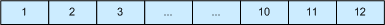
\includegraphics[width=1.0\linewidth,height=6.5in,keepaspectratio]{../images/6.png}
\end{center}
\raggedright{}\myfigurewithoutcaption{6}
\end{minipage}\vspace{0.75cm}

{\itshape The notebook (array) contains 12 pages (elements)} 
\end{center}
\setmainfont[Path=/usr/share/fonts/truetype/cmu/,UprightFont=cmunrm.ttf,BoldFont=cmunbx.ttf,ItalicFont=cmunti.ttf,BoldItalicFont=cmunbi.ttf]{cmunrm.ttf}\setmonofont[Path=/usr/share/fonts/truetype/cmu/,UprightFont=cmuntt.ttf,BoldFont=cmuntb.ttf,ItalicFont=cmunit.ttf,BoldItalicFont=cmuntx.ttf]{cmunrm.ttf}


Arrays can also be multidimensional -{} instead of accessing an element of a one-{}dimensional list, elements are accessed by two or more indices, as from a matrix or tensor.

Multidimensional arrays are as simple as our notebook example above.  To envision a multidimensional array, think of a calendar.  Each page of the calendar, 1 through 12, is an element, representing a month, which contains approximately 30 elements, which represent days.  Each day may or may not have information in it.  Programmatically then, calendar(4,15) would refer to the 4th month, 15th day.  Thus we have a two-{}dimensional array.  To envision a three-{}dimensional array, break each day up into 24 hours.  Now calendar(4,15,9) would refer to  4th month, 15th day, 9th hour.



\begin{center}


\begin{minipage}{1.0\linewidth}
\begin{center}
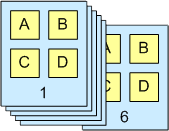
\includegraphics[width=1.0\linewidth,height=6.5in,keepaspectratio]{../images/7.png}
\end{center}
\raggedright{}\myfigurewithoutcaption{7}
\end{minipage}\vspace{0.75cm}

{\itshape A simple 6 element by 4 element array} 
\end{center}
\setmainfont[Path=/usr/share/fonts/truetype/cmu/,UprightFont=cmunrm.ttf,BoldFont=cmunbx.ttf,ItalicFont=cmunti.ttf,BoldItalicFont=cmunbi.ttf]{cmunrm.ttf}\setmonofont[Path=/usr/share/fonts/truetype/cmu/,UprightFont=cmuntt.ttf,BoldFont=cmuntb.ttf,ItalicFont=cmunit.ttf,BoldItalicFont=cmuntx.ttf]{cmunrm.ttf}

\LaTeXDoubleBoxOpenTemplate{Array{\mbox{$<$}}Element{\mbox{$>$}}}{{\ttfamily \setmainfont[Path=/usr/share/fonts/truetype/cmu/,UprightFont=cmunrm.ttf,BoldFont=cmunbx.ttf,ItalicFont=cmunti.ttf,BoldItalicFont=cmunbi.ttf]{cmuntt.ttf}\setmonofont[Path=/usr/share/fonts/truetype/cmu/,UprightFont=cmuntt.ttf,BoldFont=cmuntb.ttf,ItalicFont=cmunit.ttf,BoldItalicFont=cmuntx.ttf]{cmuntt.ttf}\ttfamily make-{}array(integer {\ttfamily \itshape n} \setmainfont[Path=/usr/share/fonts/truetype/cmu/,UprightFont=cmunrm.ttf,BoldFont=cmunbx.ttf,ItalicFont=cmunti.ttf,BoldItalicFont=cmunbi.ttf]{cmuntt.ttf}\setmonofont[Path=/usr/share/fonts/truetype/cmu/,UprightFont=cmuntt.ttf,BoldFont=cmuntb.ttf,ItalicFont=cmunit.ttf,BoldItalicFont=cmuntx.ttf]{cmuntt.ttf}\ttfamily ): Array} 
\begin{myquote}
\item{} \setmainfont[Path=/usr/share/fonts/truetype/cmu/,UprightFont=cmunrm.ttf,BoldFont=cmunbx.ttf,ItalicFont=cmunti.ttf,BoldItalicFont=cmunbi.ttf]{cmunrm.ttf}\setmonofont[Path=/usr/share/fonts/truetype/cmu/,UprightFont=cmuntt.ttf,BoldFont=cmuntb.ttf,ItalicFont=cmunit.ttf,BoldItalicFont=cmuntx.ttf]{cmunrm.ttf}Create an array of elements indexed from {$0$} to {$n-1$}, inclusive. The number of elements in the array, also known as the size of the array, is {\itshape n} \setmainfont[Path=/usr/share/fonts/truetype/cmu/,UprightFont=cmunrm.ttf,BoldFont=cmunbx.ttf,ItalicFont=cmunti.ttf,BoldItalicFont=cmunbi.ttf]{cmunrm.ttf}\setmonofont[Path=/usr/share/fonts/truetype/cmu/,UprightFont=cmuntt.ttf,BoldFont=cmuntb.ttf,ItalicFont=cmunit.ttf,BoldItalicFont=cmuntx.ttf]{cmunrm.ttf}.
{\ttfamily \setmainfont[Path=/usr/share/fonts/truetype/cmu/,UprightFont=cmunrm.ttf,BoldFont=cmunbx.ttf,ItalicFont=cmunti.ttf,BoldItalicFont=cmunbi.ttf]{cmuntt.ttf}\setmonofont[Path=/usr/share/fonts/truetype/cmu/,UprightFont=cmuntt.ttf,BoldFont=cmuntb.ttf,ItalicFont=cmunit.ttf,BoldItalicFont=cmuntx.ttf]{cmuntt.ttf}\ttfamily get-{}value-{}at(Array {\ttfamily \itshape a} \setmainfont[Path=/usr/share/fonts/truetype/cmu/,UprightFont=cmunrm.ttf,BoldFont=cmunbx.ttf,ItalicFont=cmunti.ttf,BoldItalicFont=cmunbi.ttf]{cmuntt.ttf}\setmonofont[Path=/usr/share/fonts/truetype/cmu/,UprightFont=cmuntt.ttf,BoldFont=cmuntb.ttf,ItalicFont=cmunit.ttf,BoldItalicFont=cmuntx.ttf]{cmuntt.ttf}\ttfamily , integer {\ttfamily \itshape index} \setmainfont[Path=/usr/share/fonts/truetype/cmu/,UprightFont=cmunrm.ttf,BoldFont=cmunbx.ttf,ItalicFont=cmunti.ttf,BoldItalicFont=cmunbi.ttf]{cmuntt.ttf}\setmonofont[Path=/usr/share/fonts/truetype/cmu/,UprightFont=cmuntt.ttf,BoldFont=cmuntb.ttf,ItalicFont=cmunit.ttf,BoldItalicFont=cmuntx.ttf]{cmuntt.ttf}\ttfamily ): Element} 
\item{} \setmainfont[Path=/usr/share/fonts/truetype/cmu/,UprightFont=cmunrm.ttf,BoldFont=cmunbx.ttf,ItalicFont=cmunti.ttf,BoldItalicFont=cmunbi.ttf]{cmunrm.ttf}\setmonofont[Path=/usr/share/fonts/truetype/cmu/,UprightFont=cmuntt.ttf,BoldFont=cmuntb.ttf,ItalicFont=cmunit.ttf,BoldItalicFont=cmuntx.ttf]{cmunrm.ttf}Returns the value of the element at the given {\itshape index} \setmainfont[Path=/usr/share/fonts/truetype/cmu/,UprightFont=cmunrm.ttf,BoldFont=cmunbx.ttf,ItalicFont=cmunti.ttf,BoldItalicFont=cmunbi.ttf]{cmunrm.ttf}\setmonofont[Path=/usr/share/fonts/truetype/cmu/,UprightFont=cmuntt.ttf,BoldFont=cmuntb.ttf,ItalicFont=cmunit.ttf,BoldItalicFont=cmuntx.ttf]{cmunrm.ttf}. The value of {\itshape index} \setmainfont[Path=/usr/share/fonts/truetype/cmu/,UprightFont=cmunrm.ttf,BoldFont=cmunbx.ttf,ItalicFont=cmunti.ttf,BoldItalicFont=cmunbi.ttf]{cmunrm.ttf}\setmonofont[Path=/usr/share/fonts/truetype/cmu/,UprightFont=cmuntt.ttf,BoldFont=cmuntb.ttf,ItalicFont=cmunit.ttf,BoldItalicFont=cmuntx.ttf]{cmunrm.ttf} must be in bounds: {\itshape 0 <{}= index <{}= (n -{} 1)} \setmainfont[Path=/usr/share/fonts/truetype/cmu/,UprightFont=cmunrm.ttf,BoldFont=cmunbx.ttf,ItalicFont=cmunti.ttf,BoldItalicFont=cmunbi.ttf]{cmunrm.ttf}\setmonofont[Path=/usr/share/fonts/truetype/cmu/,UprightFont=cmuntt.ttf,BoldFont=cmuntb.ttf,ItalicFont=cmunit.ttf,BoldItalicFont=cmuntx.ttf]{cmunrm.ttf}. This operation is also known as {\bfseries \setmainfont[Path=/usr/share/fonts/truetype/cmu/,UprightFont=cmunrm.ttf,BoldFont=cmunbx.ttf,ItalicFont=cmunti.ttf,BoldItalicFont=cmunbi.ttf]{cmunbx.ttf}\setmonofont[Path=/usr/share/fonts/truetype/cmu/,UprightFont=cmuntt.ttf,BoldFont=cmuntb.ttf,ItalicFont=cmunit.ttf,BoldItalicFont=cmuntx.ttf]{cmunbx.ttf}\bfseries subscripting} \setmainfont[Path=/usr/share/fonts/truetype/cmu/,UprightFont=cmunrm.ttf,BoldFont=cmunbx.ttf,ItalicFont=cmunti.ttf,BoldItalicFont=cmunbi.ttf]{cmunrm.ttf}\setmonofont[Path=/usr/share/fonts/truetype/cmu/,UprightFont=cmuntt.ttf,BoldFont=cmuntb.ttf,ItalicFont=cmunit.ttf,BoldItalicFont=cmuntx.ttf]{cmunrm.ttf}.
{\ttfamily \setmainfont[Path=/usr/share/fonts/truetype/cmu/,UprightFont=cmunrm.ttf,BoldFont=cmunbx.ttf,ItalicFont=cmunti.ttf,BoldItalicFont=cmunbi.ttf]{cmuntt.ttf}\setmonofont[Path=/usr/share/fonts/truetype/cmu/,UprightFont=cmuntt.ttf,BoldFont=cmuntb.ttf,ItalicFont=cmunit.ttf,BoldItalicFont=cmuntx.ttf]{cmuntt.ttf}\ttfamily set-{}value-{}at(Array {\ttfamily \itshape a} \setmainfont[Path=/usr/share/fonts/truetype/cmu/,UprightFont=cmunrm.ttf,BoldFont=cmunbx.ttf,ItalicFont=cmunti.ttf,BoldItalicFont=cmunbi.ttf]{cmuntt.ttf}\setmonofont[Path=/usr/share/fonts/truetype/cmu/,UprightFont=cmuntt.ttf,BoldFont=cmuntb.ttf,ItalicFont=cmunit.ttf,BoldItalicFont=cmuntx.ttf]{cmuntt.ttf}\ttfamily , integer {\ttfamily \itshape index} \setmainfont[Path=/usr/share/fonts/truetype/cmu/,UprightFont=cmunrm.ttf,BoldFont=cmunbx.ttf,ItalicFont=cmunti.ttf,BoldItalicFont=cmunbi.ttf]{cmuntt.ttf}\setmonofont[Path=/usr/share/fonts/truetype/cmu/,UprightFont=cmuntt.ttf,BoldFont=cmuntb.ttf,ItalicFont=cmunit.ttf,BoldItalicFont=cmuntx.ttf]{cmuntt.ttf}\ttfamily , Element {\ttfamily \itshape new-{}value} \setmainfont[Path=/usr/share/fonts/truetype/cmu/,UprightFont=cmunrm.ttf,BoldFont=cmunbx.ttf,ItalicFont=cmunti.ttf,BoldItalicFont=cmunbi.ttf]{cmuntt.ttf}\setmonofont[Path=/usr/share/fonts/truetype/cmu/,UprightFont=cmuntt.ttf,BoldFont=cmuntb.ttf,ItalicFont=cmunit.ttf,BoldItalicFont=cmuntx.ttf]{cmuntt.ttf}\ttfamily )} 
\item{} \setmainfont[Path=/usr/share/fonts/truetype/cmu/,UprightFont=cmunrm.ttf,BoldFont=cmunbx.ttf,ItalicFont=cmunti.ttf,BoldItalicFont=cmunbi.ttf]{cmunrm.ttf}\setmonofont[Path=/usr/share/fonts/truetype/cmu/,UprightFont=cmuntt.ttf,BoldFont=cmuntb.ttf,ItalicFont=cmunit.ttf,BoldItalicFont=cmuntx.ttf]{cmunrm.ttf}Sets the element of the array at the given {\itshape index} \setmainfont[Path=/usr/share/fonts/truetype/cmu/,UprightFont=cmunrm.ttf,BoldFont=cmunbx.ttf,ItalicFont=cmunti.ttf,BoldItalicFont=cmunbi.ttf]{cmunrm.ttf}\setmonofont[Path=/usr/share/fonts/truetype/cmu/,UprightFont=cmuntt.ttf,BoldFont=cmuntb.ttf,ItalicFont=cmunit.ttf,BoldItalicFont=cmuntx.ttf]{cmunrm.ttf} to be equal to {\itshape new-{}value} \setmainfont[Path=/usr/share/fonts/truetype/cmu/,UprightFont=cmunrm.ttf,BoldFont=cmunbx.ttf,ItalicFont=cmunti.ttf,BoldItalicFont=cmunbi.ttf]{cmunrm.ttf}\setmonofont[Path=/usr/share/fonts/truetype/cmu/,UprightFont=cmuntt.ttf,BoldFont=cmuntb.ttf,ItalicFont=cmunit.ttf,BoldItalicFont=cmuntx.ttf]{cmunrm.ttf}.

\end{myquote}}

Arrays guarantee {\bfseries \setmainfont[Path=/usr/share/fonts/truetype/cmu/,UprightFont=cmunrm.ttf,BoldFont=cmunbx.ttf,ItalicFont=cmunti.ttf,BoldItalicFont=cmunbi.ttf]{cmunbx.ttf}\setmonofont[Path=/usr/share/fonts/truetype/cmu/,UprightFont=cmuntt.ttf,BoldFont=cmuntb.ttf,ItalicFont=cmunit.ttf,BoldItalicFont=cmuntx.ttf]{cmunbx.ttf}\bfseries constant} \setmainfont[Path=/usr/share/fonts/truetype/cmu/,UprightFont=cmunrm.ttf,BoldFont=cmunbx.ttf,ItalicFont=cmunti.ttf,BoldItalicFont=cmunbi.ttf]{cmunrm.ttf}\setmonofont[Path=/usr/share/fonts/truetype/cmu/,UprightFont=cmuntt.ttf,BoldFont=cmuntb.ttf,ItalicFont=cmunit.ttf,BoldItalicFont=cmuntx.ttf]{cmunrm.ttf} time read and write access, {$O(1)$}, however many lookup operations (find\_min, find\_max, find\_index) of an instance of an element are {\bfseries \setmainfont[Path=/usr/share/fonts/truetype/cmu/,UprightFont=cmunrm.ttf,BoldFont=cmunbx.ttf,ItalicFont=cmunti.ttf,BoldItalicFont=cmunbi.ttf]{cmunbx.ttf}\setmonofont[Path=/usr/share/fonts/truetype/cmu/,UprightFont=cmuntt.ttf,BoldFont=cmuntb.ttf,ItalicFont=cmunit.ttf,BoldItalicFont=cmuntx.ttf]{cmunbx.ttf}\bfseries linear} \setmainfont[Path=/usr/share/fonts/truetype/cmu/,UprightFont=cmunrm.ttf,BoldFont=cmunbx.ttf,ItalicFont=cmunti.ttf,BoldItalicFont=cmunbi.ttf]{cmunrm.ttf}\setmonofont[Path=/usr/share/fonts/truetype/cmu/,UprightFont=cmuntt.ttf,BoldFont=cmuntb.ttf,ItalicFont=cmunit.ttf,BoldItalicFont=cmuntx.ttf]{cmunrm.ttf} time, {$O(n)$}.  Arrays are very efficient in most languages, as operations compute the address of an element via a simple formula based on the base address element of the array.

Array implementations differ greatly between languages: some languages allow arrays to be re-{}sized automatically, or to even contain elements of differing types (such as Perl).  Other languages are very strict and require the type and length information of an array to be known at run time (such as C).

Arrays typically map directly to contiguous storage locations within your computer\textquotesingle{}s memory and are therefore the \symbol{34}natural\symbol{34} storage structure for most higher level languages.

Simple linear arrays are the basis for most of the other data structures.  Many languages do not allow you to allocate any structure except an array, everything else must be implemented on top of the array.  The exception is the linked list, that is typically implemented as individually allocated objects, but it is possible to implement a linked list within an array.
\subsection{Type}
\label{21}

The array index needs to be of some type. Usually, the standard integer type of that language is used, but there are also languages such as \myhref{http://en.wikipedia.org/wiki/Ada_programming_language}{Ada} and \myhref{http://en.wikipedia.org/wiki/Pascal_programming_language}{Pascal} which allow any discrete type as an array index. Scripting languages often allow any type as an index (associative array).
\subsection{Bounds}
\label{22}

The array index consists of a range of values with a lower bound and an upper bound.

In some programming languages only the upper bound can be chosen while the lower bound is fixed to be either 0 {\small (\myhref{http://en.wikipedia.org/wiki/C_programming_language}{C}, \myhref{http://en.wikipedia.org/wiki/C_plus_plus}{C++}, \myhref{http://en.wikipedia.org/wiki/C_Sharp_programming_language}{C\#}, \myhref{http://en.wikipedia.org/wiki/Java_programming_language}{Java})} or 1 {\small (\myhref{http://en.wikibooks.org/wiki/FORTRAN\%2066}{FORTRAN 66}, \myhref{http://en.wikipedia.org/wiki/R_Programming}{R})}.

In other programming languages {\small (\myhref{http://en.wikipedia.org/wiki/Ada_programming_language}{Ada}, \myhref{http://en.wikipedia.org/wiki/PL\%2FI}{PL/I}, \myhref{http://en.wikipedia.org/wiki/Pascal_programming_language}{Pascal})} both the upper and lower bound can be freely chosen {\small (even negative)}.
\subsection{Bounds check}
\label{23}

The third aspect of an array index is the check for valid ranges and what happens when an invalid index is accessed. This is a very important point since the majority of \myhref{http://en.wikipedia.org/wiki/Computer_worm}{computer worms} and \myhref{http://en.wikipedia.org/wiki/Computer_virus}{computer viruses} attack by using invalid array bounds.

There are three options open:

\begin{myenumerate}
\item{}  Most languages {\small }(\myhref{http://en.wikipedia.org/wiki/Ada_programming_language}{Ada}, \myhref{http://en.wikipedia.org/wiki/PL\%2FI}{PL/I}, \myhref{http://en.wikipedia.org/wiki/Pascal_programming_language}{Pascal}, \myhref{http://en.wikipedia.org/wiki/Java_programming_language}{Java}, \myhref{http://en.wikipedia.org/wiki/C\%20Sharp}{C\#}){\small } will check the bounds and raise some error condition when an element is accessed which does not exist.
\item{}  A few languages {\small }(\myhref{http://en.wikipedia.org/wiki/C_programming_language}{C}, \myhref{http://en.wikipedia.org/wiki/C_plus_plus}{C++}){\small } will not check the bounds and return or set some arbitrary value when an element outside the valid range is accessed. 
\item{}  Scripting languages often automatically expand the array when data is written to an index which was not valid until then.
\end{myenumerate}

\subsection{Declaring Array Types}
\label{24}

The declaration of array type depends on how many features the array in a particular language has.

The easiest declaration is when the language has a fixed lower bound and fixed index type. If you need an array to store the monthly income you could declare in \myhref{http://en.wikibooks.org/wiki/C\%20Programming}{C}


\begin{Shaded}
\begin{Highlighting}[]

\KeywordTok{typedef}\ensuremath{\text{ }}\DataTypeTok{double}\ensuremath{\text{ }}\NormalTok{Income[}\DecValTok{12}\NormalTok{];}\newline
\end{Highlighting}
\end{Shaded}


This gives you an array with in the range of 0 to 11. For a full description of arrays in C see \myhref{http://en.wikibooks.org/wiki/C\%20Programming\%2FArrays}{C Programming/Arrays}.

If you use a language where you can choose both the lower bound as well as the index type, the declaration is -{}-{} of course -{}-{} more complex. Here are two examples in \myhref{http://en.wikibooks.org/wiki/Ada\%20Programming}{Ada}:


\begin{Shaded}
\begin{Highlighting}[]

\KeywordTok{type}\ensuremath{\text{ }}\NormalTok{Month\ensuremath{\text{ }}}\KeywordTok{is}\ensuremath{\text{ }}\KeywordTok{range}\ensuremath{\text{ }}\DecValTok{1}\ensuremath{\text{ }}\NormalTok{..\ensuremath{\text{ }}}\DecValTok{12}\NormalTok{;}\newline
\KeywordTok{type}\ensuremath{\text{ }}\NormalTok{Income\ensuremath{\text{ }}}\KeywordTok{is}\ensuremath{\text{ }}\KeywordTok{array}\NormalTok{(Month)\ensuremath{\text{ }}}\KeywordTok{of}\ensuremath{\text{ }}\DataTypeTok{Float}\NormalTok{;}\newline
\end{Highlighting}
\end{Shaded}


or shorter:


\begin{Shaded}
\begin{Highlighting}[]

\KeywordTok{type}\ensuremath{\text{ }}\NormalTok{Income\ensuremath{\text{ }}}\KeywordTok{is}\ensuremath{\text{ }}\KeywordTok{array}\NormalTok{(}\DecValTok{1}\ensuremath{\text{ }}\NormalTok{..\ensuremath{\text{ }}}\DecValTok{12}\NormalTok{)\ensuremath{\text{ }}}\KeywordTok{of}\ensuremath{\text{ }}\DataTypeTok{Float}\NormalTok{;}\newline
\end{Highlighting}
\end{Shaded}


For a full description of arrays in Ada see \myhref{http://en.wikibooks.org/wiki/Ada\%20Programming\%2FTypes\%2Farray}{Ada Programming/Types/array}.
\subsection{Array Access}
\label{25}

We generally write arrays with a name, followed by the index in some brackets, square \textquotesingle{}{$\text{[}$}{$\text{]}$}\textquotesingle{} or round \textquotesingle{}()\textquotesingle{}.  For example, {\ttfamily \setmainfont[Path=/usr/share/fonts/truetype/cmu/,UprightFont=cmunrm.ttf,BoldFont=cmunbx.ttf,ItalicFont=cmunti.ttf,BoldItalicFont=cmunbi.ttf]{cmuntt.ttf}\setmonofont[Path=/usr/share/fonts/truetype/cmu/,UprightFont=cmuntt.ttf,BoldFont=cmuntb.ttf,ItalicFont=cmunit.ttf,BoldItalicFont=cmuntx.ttf]{cmuntt.ttf}\ttfamily august{$\text{[}$}3{$\text{]}$}} \setmainfont[Path=/usr/share/fonts/truetype/cmu/,UprightFont=cmunrm.ttf,BoldFont=cmunbx.ttf,ItalicFont=cmunti.ttf,BoldItalicFont=cmunbi.ttf]{cmunrm.ttf}\setmonofont[Path=/usr/share/fonts/truetype/cmu/,UprightFont=cmuntt.ttf,BoldFont=cmuntb.ttf,ItalicFont=cmunit.ttf,BoldItalicFont=cmuntx.ttf]{cmunrm.ttf} is the method used in the C programming language to refer to a particular day in the month.

Because the C language starts the index at zero, {\ttfamily \setmainfont[Path=/usr/share/fonts/truetype/cmu/,UprightFont=cmunrm.ttf,BoldFont=cmunbx.ttf,ItalicFont=cmunti.ttf,BoldItalicFont=cmunbi.ttf]{cmuntt.ttf}\setmonofont[Path=/usr/share/fonts/truetype/cmu/,UprightFont=cmuntt.ttf,BoldFont=cmuntb.ttf,ItalicFont=cmunit.ttf,BoldItalicFont=cmuntx.ttf]{cmuntt.ttf}\ttfamily august{$\text{[}$}3{$\text{]}$}} \setmainfont[Path=/usr/share/fonts/truetype/cmu/,UprightFont=cmunrm.ttf,BoldFont=cmunbx.ttf,ItalicFont=cmunti.ttf,BoldItalicFont=cmunbi.ttf]{cmunrm.ttf}\setmonofont[Path=/usr/share/fonts/truetype/cmu/,UprightFont=cmuntt.ttf,BoldFont=cmuntb.ttf,ItalicFont=cmunit.ttf,BoldItalicFont=cmuntx.ttf]{cmunrm.ttf} is the 4th element in the array.  {\ttfamily \setmainfont[Path=/usr/share/fonts/truetype/cmu/,UprightFont=cmunrm.ttf,BoldFont=cmunbx.ttf,ItalicFont=cmunti.ttf,BoldItalicFont=cmunbi.ttf]{cmuntt.ttf}\setmonofont[Path=/usr/share/fonts/truetype/cmu/,UprightFont=cmuntt.ttf,BoldFont=cmuntb.ttf,ItalicFont=cmunit.ttf,BoldItalicFont=cmuntx.ttf]{cmuntt.ttf}\ttfamily august{$\text{[}$}0{$\text{]}$}} \setmainfont[Path=/usr/share/fonts/truetype/cmu/,UprightFont=cmunrm.ttf,BoldFont=cmunbx.ttf,ItalicFont=cmunti.ttf,BoldItalicFont=cmunbi.ttf]{cmunrm.ttf}\setmonofont[Path=/usr/share/fonts/truetype/cmu/,UprightFont=cmuntt.ttf,BoldFont=cmuntb.ttf,ItalicFont=cmunit.ttf,BoldItalicFont=cmuntx.ttf]{cmunrm.ttf} actually refers to the first element of this array.  Starting an index at zero is natural for computers, whose internal representations of numbers begin with zero, but for humans, this unnatural numbering system can lead to problems when accessing data in an array.  When fetching an element in a language with zero-{}based indexes, keep in mind the {\itshape true} \setmainfont[Path=/usr/share/fonts/truetype/cmu/,UprightFont=cmunrm.ttf,BoldFont=cmunbx.ttf,ItalicFont=cmunti.ttf,BoldItalicFont=cmunbi.ttf]{cmunrm.ttf}\setmonofont[Path=/usr/share/fonts/truetype/cmu/,UprightFont=cmuntt.ttf,BoldFont=cmuntb.ttf,ItalicFont=cmunit.ttf,BoldItalicFont=cmuntx.ttf]{cmunrm.ttf} length of an array, lest you find yourself fetching the wrong data.  This is the disadvantage of programming in languages with fixed lower bounds, the programmer must always remember that \symbol{34}{$\text{[}$}0{$\text{]}$}\symbol{34} means \symbol{34}1st\symbol{34} and, when appropriate, add or subtract one from the index.  Languages with variable lower bounds will take that burden off the programmer\textquotesingle{}s shoulder.

We use indexes to store {\itshape related} \setmainfont[Path=/usr/share/fonts/truetype/cmu/,UprightFont=cmunrm.ttf,BoldFont=cmunbx.ttf,ItalicFont=cmunti.ttf,BoldItalicFont=cmunbi.ttf]{cmunrm.ttf}\setmonofont[Path=/usr/share/fonts/truetype/cmu/,UprightFont=cmuntt.ttf,BoldFont=cmuntb.ttf,ItalicFont=cmunit.ttf,BoldItalicFont=cmuntx.ttf]{cmunrm.ttf} data. If our C language array is called {\ttfamily \setmainfont[Path=/usr/share/fonts/truetype/cmu/,UprightFont=cmunrm.ttf,BoldFont=cmunbx.ttf,ItalicFont=cmunti.ttf,BoldItalicFont=cmunbi.ttf]{cmuntt.ttf}\setmonofont[Path=/usr/share/fonts/truetype/cmu/,UprightFont=cmuntt.ttf,BoldFont=cmuntb.ttf,ItalicFont=cmunit.ttf,BoldItalicFont=cmuntx.ttf]{cmuntt.ttf}\ttfamily august} \setmainfont[Path=/usr/share/fonts/truetype/cmu/,UprightFont=cmunrm.ttf,BoldFont=cmunbx.ttf,ItalicFont=cmunti.ttf,BoldItalicFont=cmunbi.ttf]{cmunrm.ttf}\setmonofont[Path=/usr/share/fonts/truetype/cmu/,UprightFont=cmuntt.ttf,BoldFont=cmuntb.ttf,ItalicFont=cmunit.ttf,BoldItalicFont=cmuntx.ttf]{cmunrm.ttf}, and we wish to store that we\textquotesingle{}re going to the supermarket on the 1st, we can say, for example
\\

\TemplateSpaceIndent{$\text{ }${}august{$\text{[}$}0{$\text{]}$}$\text{ }${}=$\text{ }${}\symbol{34}Going$\text{ }${}to$\text{ }${}the$\text{ }${}shops$\text{ }${}today\symbol{34}}


In this way, we can go through the indexes from 0 to 30 and get the related tasks for each day in {\ttfamily \setmainfont[Path=/usr/share/fonts/truetype/cmu/,UprightFont=cmunrm.ttf,BoldFont=cmunbx.ttf,ItalicFont=cmunti.ttf,BoldItalicFont=cmunbi.ttf]{cmuntt.ttf}\setmonofont[Path=/usr/share/fonts/truetype/cmu/,UprightFont=cmuntt.ttf,BoldFont=cmuntb.ttf,ItalicFont=cmunit.ttf,BoldItalicFont=cmuntx.ttf]{cmuntt.ttf}\ttfamily august} \setmainfont[Path=/usr/share/fonts/truetype/cmu/,UprightFont=cmunrm.ttf,BoldFont=cmunbx.ttf,ItalicFont=cmunti.ttf,BoldItalicFont=cmunbi.ttf]{cmunrm.ttf}\setmonofont[Path=/usr/share/fonts/truetype/cmu/,UprightFont=cmuntt.ttf,BoldFont=cmuntb.ttf,ItalicFont=cmunit.ttf,BoldItalicFont=cmuntx.ttf]{cmunrm.ttf}.

\LaTeXNullTemplate{}
\LaTeXNullTemplate{}

\label{26}
\LaTeXNullTemplate{}
\section{List Structures and Iterators}
\label{27}
We have seen now two different data structures that allow us to store an ordered sequence of elements. However, they have two very different interfaces. The array allows us to use {\ttfamily \setmainfont[Path=/usr/share/fonts/truetype/cmu/,UprightFont=cmunrm.ttf,BoldFont=cmunbx.ttf,ItalicFont=cmunti.ttf,BoldItalicFont=cmunbi.ttf]{cmuntt.ttf}\setmonofont[Path=/usr/share/fonts/truetype/cmu/,UprightFont=cmuntt.ttf,BoldFont=cmuntb.ttf,ItalicFont=cmunit.ttf,BoldItalicFont=cmuntx.ttf]{cmuntt.ttf}\ttfamily get-{}element()} \setmainfont[Path=/usr/share/fonts/truetype/cmu/,UprightFont=cmunrm.ttf,BoldFont=cmunbx.ttf,ItalicFont=cmunti.ttf,BoldItalicFont=cmunbi.ttf]{cmunrm.ttf}\setmonofont[Path=/usr/share/fonts/truetype/cmu/,UprightFont=cmuntt.ttf,BoldFont=cmuntb.ttf,ItalicFont=cmunit.ttf,BoldItalicFont=cmuntx.ttf]{cmunrm.ttf} and {\ttfamily \setmainfont[Path=/usr/share/fonts/truetype/cmu/,UprightFont=cmunrm.ttf,BoldFont=cmunbx.ttf,ItalicFont=cmunti.ttf,BoldItalicFont=cmunbi.ttf]{cmuntt.ttf}\setmonofont[Path=/usr/share/fonts/truetype/cmu/,UprightFont=cmuntt.ttf,BoldFont=cmuntb.ttf,ItalicFont=cmunit.ttf,BoldItalicFont=cmuntx.ttf]{cmuntt.ttf}\ttfamily set-{}element()} \setmainfont[Path=/usr/share/fonts/truetype/cmu/,UprightFont=cmunrm.ttf,BoldFont=cmunbx.ttf,ItalicFont=cmunti.ttf,BoldItalicFont=cmunbi.ttf]{cmunrm.ttf}\setmonofont[Path=/usr/share/fonts/truetype/cmu/,UprightFont=cmuntt.ttf,BoldFont=cmuntb.ttf,ItalicFont=cmunit.ttf,BoldItalicFont=cmuntx.ttf]{cmunrm.ttf} functions to access and change elements. The node chain requires us to use {\ttfamily \setmainfont[Path=/usr/share/fonts/truetype/cmu/,UprightFont=cmunrm.ttf,BoldFont=cmunbx.ttf,ItalicFont=cmunti.ttf,BoldItalicFont=cmunbi.ttf]{cmuntt.ttf}\setmonofont[Path=/usr/share/fonts/truetype/cmu/,UprightFont=cmuntt.ttf,BoldFont=cmuntb.ttf,ItalicFont=cmunit.ttf,BoldItalicFont=cmuntx.ttf]{cmuntt.ttf}\ttfamily get-{}next()} \setmainfont[Path=/usr/share/fonts/truetype/cmu/,UprightFont=cmunrm.ttf,BoldFont=cmunbx.ttf,ItalicFont=cmunti.ttf,BoldItalicFont=cmunbi.ttf]{cmunrm.ttf}\setmonofont[Path=/usr/share/fonts/truetype/cmu/,UprightFont=cmuntt.ttf,BoldFont=cmuntb.ttf,ItalicFont=cmunit.ttf,BoldItalicFont=cmuntx.ttf]{cmunrm.ttf} until we find the desired node, and then we can use {\ttfamily \setmainfont[Path=/usr/share/fonts/truetype/cmu/,UprightFont=cmunrm.ttf,BoldFont=cmunbx.ttf,ItalicFont=cmunti.ttf,BoldItalicFont=cmunbi.ttf]{cmuntt.ttf}\setmonofont[Path=/usr/share/fonts/truetype/cmu/,UprightFont=cmuntt.ttf,BoldFont=cmuntb.ttf,ItalicFont=cmunit.ttf,BoldItalicFont=cmuntx.ttf]{cmuntt.ttf}\ttfamily get-{}value()} \setmainfont[Path=/usr/share/fonts/truetype/cmu/,UprightFont=cmunrm.ttf,BoldFont=cmunbx.ttf,ItalicFont=cmunti.ttf,BoldItalicFont=cmunbi.ttf]{cmunrm.ttf}\setmonofont[Path=/usr/share/fonts/truetype/cmu/,UprightFont=cmuntt.ttf,BoldFont=cmuntb.ttf,ItalicFont=cmunit.ttf,BoldItalicFont=cmuntx.ttf]{cmunrm.ttf} and {\ttfamily \setmainfont[Path=/usr/share/fonts/truetype/cmu/,UprightFont=cmunrm.ttf,BoldFont=cmunbx.ttf,ItalicFont=cmunti.ttf,BoldItalicFont=cmunbi.ttf]{cmuntt.ttf}\setmonofont[Path=/usr/share/fonts/truetype/cmu/,UprightFont=cmuntt.ttf,BoldFont=cmuntb.ttf,ItalicFont=cmunit.ttf,BoldItalicFont=cmuntx.ttf]{cmuntt.ttf}\ttfamily set-{}value()} \setmainfont[Path=/usr/share/fonts/truetype/cmu/,UprightFont=cmunrm.ttf,BoldFont=cmunbx.ttf,ItalicFont=cmunti.ttf,BoldItalicFont=cmunbi.ttf]{cmunrm.ttf}\setmonofont[Path=/usr/share/fonts/truetype/cmu/,UprightFont=cmuntt.ttf,BoldFont=cmuntb.ttf,ItalicFont=cmunit.ttf,BoldItalicFont=cmuntx.ttf]{cmunrm.ttf} to access and modify its value. Now, what if you\textquotesingle{}ve written some code, and you realize that you should have been using the other sequence data structure? You have to go through all of the code you\textquotesingle{}ve already written and change one set of accessor functions into another. What a pain! Fortunately, there is a way to localize this change into only one place: by using the {\bfseries \setmainfont[Path=/usr/share/fonts/truetype/cmu/,UprightFont=cmunrm.ttf,BoldFont=cmunbx.ttf,ItalicFont=cmunti.ttf,BoldItalicFont=cmunbi.ttf]{cmunbx.ttf}\setmonofont[Path=/usr/share/fonts/truetype/cmu/,UprightFont=cmuntt.ttf,BoldFont=cmuntb.ttf,ItalicFont=cmunit.ttf,BoldItalicFont=cmuntx.ttf]{cmunbx.ttf}\bfseries List} \setmainfont[Path=/usr/share/fonts/truetype/cmu/,UprightFont=cmunrm.ttf,BoldFont=cmunbx.ttf,ItalicFont=cmunti.ttf,BoldItalicFont=cmunbi.ttf]{cmunrm.ttf}\setmonofont[Path=/usr/share/fonts/truetype/cmu/,UprightFont=cmuntt.ttf,BoldFont=cmuntb.ttf,ItalicFont=cmunit.ttf,BoldItalicFont=cmuntx.ttf]{cmunrm.ttf} Abstract Data Type (ADT).

\LaTeXShadedColorBoxTemplate{\definecolor{shadecolor}{rgb}{1.00000,1.00000,0.93333}}{
{\bfseries {\ttfamily \setmainfont[Path=/usr/share/fonts/truetype/cmu/,UprightFont=cmunrm.ttf,BoldFont=cmunbx.ttf,ItalicFont=cmunti.ttf,BoldItalicFont=cmunbi.ttf]{cmuntb.ttf}\setmonofont[Path=/usr/share/fonts/truetype/cmu/,UprightFont=cmuntt.ttf,BoldFont=cmuntb.ttf,ItalicFont=cmunit.ttf,BoldItalicFont=cmuntx.ttf]{cmuntb.ttf}\ttfamily \bfseries List<{}item-{}type>{}} \setmainfont[Path=/usr/share/fonts/truetype/cmu/,UprightFont=cmunrm.ttf,BoldFont=cmunbx.ttf,ItalicFont=cmunti.ttf,BoldItalicFont=cmunbi.ttf]{cmunbx.ttf}\setmonofont[Path=/usr/share/fonts/truetype/cmu/,UprightFont=cmuntt.ttf,BoldFont=cmuntb.ttf,ItalicFont=cmunit.ttf,BoldItalicFont=cmuntx.ttf]{cmunbx.ttf}\bfseries  ADT} \setmainfont[Path=/usr/share/fonts/truetype/cmu/,UprightFont=cmunrm.ttf,BoldFont=cmunbx.ttf,ItalicFont=cmunti.ttf,BoldItalicFont=cmunbi.ttf]{cmunrm.ttf}\setmonofont[Path=/usr/share/fonts/truetype/cmu/,UprightFont=cmuntt.ttf,BoldFont=cmuntb.ttf,ItalicFont=cmunit.ttf,BoldItalicFont=cmuntx.ttf]{cmunrm.ttf}

{\bfseries {\ttfamily {\bfseries \setmainfont[Path=/usr/share/fonts/truetype/cmu/,UprightFont=cmunrm.ttf,BoldFont=cmunbx.ttf,ItalicFont=cmunti.ttf,BoldItalicFont=cmunbi.ttf]{cmuntb.ttf}\setmonofont[Path=/usr/share/fonts/truetype/cmu/,UprightFont=cmuntt.ttf,BoldFont=cmuntb.ttf,ItalicFont=cmunit.ttf,BoldItalicFont=cmuntx.ttf]{cmuntb.ttf}\ttfamily \bfseries get-{}begin} ():List Iterator<{}item-{}type>{}}} \setmainfont[Path=/usr/share/fonts/truetype/cmu/,UprightFont=cmunrm.ttf,BoldFont=cmunbx.ttf,ItalicFont=cmunti.ttf,BoldItalicFont=cmunbi.ttf]{cmunrm.ttf}\setmonofont[Path=/usr/share/fonts/truetype/cmu/,UprightFont=cmuntt.ttf,BoldFont=cmuntb.ttf,ItalicFont=cmunit.ttf,BoldItalicFont=cmuntx.ttf]{cmunrm.ttf}

\begin{myquote}
\item{}Returns the {\itshape list iterator} \setmainfont[Path=/usr/share/fonts/truetype/cmu/,UprightFont=cmunrm.ttf,BoldFont=cmunbx.ttf,ItalicFont=cmunti.ttf,BoldItalicFont=cmunbi.ttf]{cmunrm.ttf}\setmonofont[Path=/usr/share/fonts/truetype/cmu/,UprightFont=cmuntt.ttf,BoldFont=cmuntb.ttf,ItalicFont=cmunit.ttf,BoldItalicFont=cmuntx.ttf]{cmunrm.ttf} (we\textquotesingle{}ll define this soon) that represents the first element of the list. Runs in {$O(1)$} time.
\end{myquote}

{\bfseries {\ttfamily {\bfseries \setmainfont[Path=/usr/share/fonts/truetype/cmu/,UprightFont=cmunrm.ttf,BoldFont=cmunbx.ttf,ItalicFont=cmunti.ttf,BoldItalicFont=cmunbi.ttf]{cmuntb.ttf}\setmonofont[Path=/usr/share/fonts/truetype/cmu/,UprightFont=cmuntt.ttf,BoldFont=cmuntb.ttf,ItalicFont=cmunit.ttf,BoldItalicFont=cmuntx.ttf]{cmuntb.ttf}\ttfamily \bfseries get-{}end} ():List Iterator<{}item-{}type>{}}} \setmainfont[Path=/usr/share/fonts/truetype/cmu/,UprightFont=cmunrm.ttf,BoldFont=cmunbx.ttf,ItalicFont=cmunti.ttf,BoldItalicFont=cmunbi.ttf]{cmunrm.ttf}\setmonofont[Path=/usr/share/fonts/truetype/cmu/,UprightFont=cmuntt.ttf,BoldFont=cmuntb.ttf,ItalicFont=cmunit.ttf,BoldItalicFont=cmuntx.ttf]{cmunrm.ttf}

\begin{myquote}
\item{}Returns the list iterator that represents one element past the last element in the list. Runs in {$O(1)$} time.
\end{myquote}

{\bfseries {\ttfamily {\bfseries \setmainfont[Path=/usr/share/fonts/truetype/cmu/,UprightFont=cmunrm.ttf,BoldFont=cmunbx.ttf,ItalicFont=cmunti.ttf,BoldItalicFont=cmunbi.ttf]{cmuntb.ttf}\setmonofont[Path=/usr/share/fonts/truetype/cmu/,UprightFont=cmuntt.ttf,BoldFont=cmuntb.ttf,ItalicFont=cmunit.ttf,BoldItalicFont=cmuntx.ttf]{cmuntb.ttf}\ttfamily \bfseries prepend} ({\ttfamily \bfseries \itshape new-{}item} \setmainfont[Path=/usr/share/fonts/truetype/cmu/,UprightFont=cmunrm.ttf,BoldFont=cmunbx.ttf,ItalicFont=cmunti.ttf,BoldItalicFont=cmunbi.ttf]{cmuntb.ttf}\setmonofont[Path=/usr/share/fonts/truetype/cmu/,UprightFont=cmuntt.ttf,BoldFont=cmuntb.ttf,ItalicFont=cmunit.ttf,BoldItalicFont=cmuntx.ttf]{cmuntb.ttf}\ttfamily \bfseries :item-{}type)}} \setmainfont[Path=/usr/share/fonts/truetype/cmu/,UprightFont=cmunrm.ttf,BoldFont=cmunbx.ttf,ItalicFont=cmunti.ttf,BoldItalicFont=cmunbi.ttf]{cmunrm.ttf}\setmonofont[Path=/usr/share/fonts/truetype/cmu/,UprightFont=cmuntt.ttf,BoldFont=cmuntb.ttf,ItalicFont=cmunit.ttf,BoldItalicFont=cmuntx.ttf]{cmunrm.ttf}

\begin{myquote}
\item{}Adds a new element at the beginning of a list. Runs in {$O(1)$} time.
\end{myquote}

{\bfseries {\ttfamily {\bfseries \setmainfont[Path=/usr/share/fonts/truetype/cmu/,UprightFont=cmunrm.ttf,BoldFont=cmunbx.ttf,ItalicFont=cmunti.ttf,BoldItalicFont=cmunbi.ttf]{cmuntb.ttf}\setmonofont[Path=/usr/share/fonts/truetype/cmu/,UprightFont=cmuntt.ttf,BoldFont=cmuntb.ttf,ItalicFont=cmunit.ttf,BoldItalicFont=cmuntx.ttf]{cmuntb.ttf}\ttfamily \bfseries insert-{}after} ({\ttfamily \bfseries \itshape iter} \setmainfont[Path=/usr/share/fonts/truetype/cmu/,UprightFont=cmunrm.ttf,BoldFont=cmunbx.ttf,ItalicFont=cmunti.ttf,BoldItalicFont=cmunbi.ttf]{cmuntb.ttf}\setmonofont[Path=/usr/share/fonts/truetype/cmu/,UprightFont=cmuntt.ttf,BoldFont=cmuntb.ttf,ItalicFont=cmunit.ttf,BoldItalicFont=cmuntx.ttf]{cmuntb.ttf}\ttfamily \bfseries :List Iterator<{}item-{}type>{}, {\ttfamily \bfseries \itshape new-{}item} \setmainfont[Path=/usr/share/fonts/truetype/cmu/,UprightFont=cmunrm.ttf,BoldFont=cmunbx.ttf,ItalicFont=cmunti.ttf,BoldItalicFont=cmunbi.ttf]{cmuntb.ttf}\setmonofont[Path=/usr/share/fonts/truetype/cmu/,UprightFont=cmuntt.ttf,BoldFont=cmuntb.ttf,ItalicFont=cmunit.ttf,BoldItalicFont=cmuntx.ttf]{cmuntb.ttf}\ttfamily \bfseries :item-{}type)}} \setmainfont[Path=/usr/share/fonts/truetype/cmu/,UprightFont=cmunrm.ttf,BoldFont=cmunbx.ttf,ItalicFont=cmunti.ttf,BoldItalicFont=cmunbi.ttf]{cmunrm.ttf}\setmonofont[Path=/usr/share/fonts/truetype/cmu/,UprightFont=cmuntt.ttf,BoldFont=cmuntb.ttf,ItalicFont=cmunit.ttf,BoldItalicFont=cmuntx.ttf]{cmunrm.ttf}

\begin{myquote}
\item{}Adds a new element immediately after {\itshape iter} \setmainfont[Path=/usr/share/fonts/truetype/cmu/,UprightFont=cmunrm.ttf,BoldFont=cmunbx.ttf,ItalicFont=cmunti.ttf,BoldItalicFont=cmunbi.ttf]{cmunrm.ttf}\setmonofont[Path=/usr/share/fonts/truetype/cmu/,UprightFont=cmuntt.ttf,BoldFont=cmuntb.ttf,ItalicFont=cmunit.ttf,BoldItalicFont=cmuntx.ttf]{cmunrm.ttf}. Runs in {$O(N)$} time.
\end{myquote}

{\bfseries {\ttfamily {\bfseries \setmainfont[Path=/usr/share/fonts/truetype/cmu/,UprightFont=cmunrm.ttf,BoldFont=cmunbx.ttf,ItalicFont=cmunti.ttf,BoldItalicFont=cmunbi.ttf]{cmuntb.ttf}\setmonofont[Path=/usr/share/fonts/truetype/cmu/,UprightFont=cmuntt.ttf,BoldFont=cmuntb.ttf,ItalicFont=cmunit.ttf,BoldItalicFont=cmuntx.ttf]{cmuntb.ttf}\ttfamily \bfseries remove-{}first} ()}} \setmainfont[Path=/usr/share/fonts/truetype/cmu/,UprightFont=cmunrm.ttf,BoldFont=cmunbx.ttf,ItalicFont=cmunti.ttf,BoldItalicFont=cmunbi.ttf]{cmunrm.ttf}\setmonofont[Path=/usr/share/fonts/truetype/cmu/,UprightFont=cmuntt.ttf,BoldFont=cmuntb.ttf,ItalicFont=cmunit.ttf,BoldItalicFont=cmuntx.ttf]{cmunrm.ttf}

\begin{myquote}
\item{}Removes the element at the beginning of a list. Runs in {$O(1)$} time.
\end{myquote}

{\bfseries {\ttfamily {\bfseries \setmainfont[Path=/usr/share/fonts/truetype/cmu/,UprightFont=cmunrm.ttf,BoldFont=cmunbx.ttf,ItalicFont=cmunti.ttf,BoldItalicFont=cmunbi.ttf]{cmuntb.ttf}\setmonofont[Path=/usr/share/fonts/truetype/cmu/,UprightFont=cmuntt.ttf,BoldFont=cmuntb.ttf,ItalicFont=cmunit.ttf,BoldItalicFont=cmuntx.ttf]{cmuntb.ttf}\ttfamily \bfseries remove-{}after} ({\ttfamily \bfseries \itshape iter} \setmainfont[Path=/usr/share/fonts/truetype/cmu/,UprightFont=cmunrm.ttf,BoldFont=cmunbx.ttf,ItalicFont=cmunti.ttf,BoldItalicFont=cmunbi.ttf]{cmuntb.ttf}\setmonofont[Path=/usr/share/fonts/truetype/cmu/,UprightFont=cmuntt.ttf,BoldFont=cmuntb.ttf,ItalicFont=cmunit.ttf,BoldItalicFont=cmuntx.ttf]{cmuntb.ttf}\ttfamily \bfseries :List Iterator<{}item-{}type>{})}} \setmainfont[Path=/usr/share/fonts/truetype/cmu/,UprightFont=cmunrm.ttf,BoldFont=cmunbx.ttf,ItalicFont=cmunti.ttf,BoldItalicFont=cmunbi.ttf]{cmunrm.ttf}\setmonofont[Path=/usr/share/fonts/truetype/cmu/,UprightFont=cmuntt.ttf,BoldFont=cmuntb.ttf,ItalicFont=cmunit.ttf,BoldItalicFont=cmuntx.ttf]{cmunrm.ttf}

\begin{myquote}
\item{}Removes the element immediately after {\itshape iter} \setmainfont[Path=/usr/share/fonts/truetype/cmu/,UprightFont=cmunrm.ttf,BoldFont=cmunbx.ttf,ItalicFont=cmunti.ttf,BoldItalicFont=cmunbi.ttf]{cmunrm.ttf}\setmonofont[Path=/usr/share/fonts/truetype/cmu/,UprightFont=cmuntt.ttf,BoldFont=cmuntb.ttf,ItalicFont=cmunit.ttf,BoldItalicFont=cmuntx.ttf]{cmunrm.ttf}. Runs in {$O(N)$} time.
\end{myquote}

{\bfseries {\ttfamily {\bfseries \setmainfont[Path=/usr/share/fonts/truetype/cmu/,UprightFont=cmunrm.ttf,BoldFont=cmunbx.ttf,ItalicFont=cmunti.ttf,BoldItalicFont=cmunbi.ttf]{cmuntb.ttf}\setmonofont[Path=/usr/share/fonts/truetype/cmu/,UprightFont=cmuntt.ttf,BoldFont=cmuntb.ttf,ItalicFont=cmunit.ttf,BoldItalicFont=cmuntx.ttf]{cmuntb.ttf}\ttfamily \bfseries is-{}empty} ():Boolean}} \setmainfont[Path=/usr/share/fonts/truetype/cmu/,UprightFont=cmunrm.ttf,BoldFont=cmunbx.ttf,ItalicFont=cmunti.ttf,BoldItalicFont=cmunbi.ttf]{cmunrm.ttf}\setmonofont[Path=/usr/share/fonts/truetype/cmu/,UprightFont=cmuntt.ttf,BoldFont=cmuntb.ttf,ItalicFont=cmunit.ttf,BoldItalicFont=cmuntx.ttf]{cmunrm.ttf}

\begin{myquote}
\item{}True if there are no elements in the list. Has a default implementation. Runs in {$O(1)$} time.
\end{myquote}

{\bfseries {\ttfamily {\bfseries \setmainfont[Path=/usr/share/fonts/truetype/cmu/,UprightFont=cmunrm.ttf,BoldFont=cmunbx.ttf,ItalicFont=cmunti.ttf,BoldItalicFont=cmunbi.ttf]{cmuntb.ttf}\setmonofont[Path=/usr/share/fonts/truetype/cmu/,UprightFont=cmuntt.ttf,BoldFont=cmuntb.ttf,ItalicFont=cmunit.ttf,BoldItalicFont=cmuntx.ttf]{cmuntb.ttf}\ttfamily \bfseries get-{}size} ():Integer}} \setmainfont[Path=/usr/share/fonts/truetype/cmu/,UprightFont=cmunrm.ttf,BoldFont=cmunbx.ttf,ItalicFont=cmunti.ttf,BoldItalicFont=cmunbi.ttf]{cmunrm.ttf}\setmonofont[Path=/usr/share/fonts/truetype/cmu/,UprightFont=cmuntt.ttf,BoldFont=cmuntb.ttf,ItalicFont=cmunit.ttf,BoldItalicFont=cmuntx.ttf]{cmunrm.ttf}

\begin{myquote}
\item{}Returns the number of elements in the list. Has a default implementation. Runs in {$O(N)$} time.
\end{myquote}


{\bfseries {\ttfamily {\bfseries \setmainfont[Path=/usr/share/fonts/truetype/cmu/,UprightFont=cmunrm.ttf,BoldFont=cmunbx.ttf,ItalicFont=cmunti.ttf,BoldItalicFont=cmunbi.ttf]{cmuntb.ttf}\setmonofont[Path=/usr/share/fonts/truetype/cmu/,UprightFont=cmuntt.ttf,BoldFont=cmuntb.ttf,ItalicFont=cmunit.ttf,BoldItalicFont=cmuntx.ttf]{cmuntb.ttf}\ttfamily \bfseries get-{}nth} ({\ttfamily \bfseries \itshape n} \setmainfont[Path=/usr/share/fonts/truetype/cmu/,UprightFont=cmunrm.ttf,BoldFont=cmunbx.ttf,ItalicFont=cmunti.ttf,BoldItalicFont=cmunbi.ttf]{cmuntb.ttf}\setmonofont[Path=/usr/share/fonts/truetype/cmu/,UprightFont=cmuntt.ttf,BoldFont=cmuntb.ttf,ItalicFont=cmunit.ttf,BoldItalicFont=cmuntx.ttf]{cmuntb.ttf}\ttfamily \bfseries :Integer):item-{}type}} \setmainfont[Path=/usr/share/fonts/truetype/cmu/,UprightFont=cmunrm.ttf,BoldFont=cmunbx.ttf,ItalicFont=cmunti.ttf,BoldItalicFont=cmunbi.ttf]{cmunrm.ttf}\setmonofont[Path=/usr/share/fonts/truetype/cmu/,UprightFont=cmuntt.ttf,BoldFont=cmuntb.ttf,ItalicFont=cmunit.ttf,BoldItalicFont=cmuntx.ttf]{cmunrm.ttf}

\begin{myquote}
\item{}Returns the nth element in the list, counting from 0. Has a default implementation. Runs in {$O(N)$} time.
\end{myquote}

{\bfseries {\ttfamily {\bfseries \setmainfont[Path=/usr/share/fonts/truetype/cmu/,UprightFont=cmunrm.ttf,BoldFont=cmunbx.ttf,ItalicFont=cmunti.ttf,BoldItalicFont=cmunbi.ttf]{cmuntb.ttf}\setmonofont[Path=/usr/share/fonts/truetype/cmu/,UprightFont=cmuntt.ttf,BoldFont=cmuntb.ttf,ItalicFont=cmunit.ttf,BoldItalicFont=cmuntx.ttf]{cmuntb.ttf}\ttfamily \bfseries set-{}nth} ({\ttfamily \bfseries \itshape n} \setmainfont[Path=/usr/share/fonts/truetype/cmu/,UprightFont=cmunrm.ttf,BoldFont=cmunbx.ttf,ItalicFont=cmunti.ttf,BoldItalicFont=cmunbi.ttf]{cmuntb.ttf}\setmonofont[Path=/usr/share/fonts/truetype/cmu/,UprightFont=cmuntt.ttf,BoldFont=cmuntb.ttf,ItalicFont=cmunit.ttf,BoldItalicFont=cmuntx.ttf]{cmuntb.ttf}\ttfamily \bfseries :Integer, {\ttfamily \bfseries \itshape new-{}value} \setmainfont[Path=/usr/share/fonts/truetype/cmu/,UprightFont=cmunrm.ttf,BoldFont=cmunbx.ttf,ItalicFont=cmunti.ttf,BoldItalicFont=cmunbi.ttf]{cmuntb.ttf}\setmonofont[Path=/usr/share/fonts/truetype/cmu/,UprightFont=cmuntt.ttf,BoldFont=cmuntb.ttf,ItalicFont=cmunit.ttf,BoldItalicFont=cmuntx.ttf]{cmuntb.ttf}\ttfamily \bfseries :item-{}type)}} \setmainfont[Path=/usr/share/fonts/truetype/cmu/,UprightFont=cmunrm.ttf,BoldFont=cmunbx.ttf,ItalicFont=cmunti.ttf,BoldItalicFont=cmunbi.ttf]{cmunrm.ttf}\setmonofont[Path=/usr/share/fonts/truetype/cmu/,UprightFont=cmuntt.ttf,BoldFont=cmuntb.ttf,ItalicFont=cmunit.ttf,BoldItalicFont=cmuntx.ttf]{cmunrm.ttf}

\begin{myquote}
\item{}Assigns a new value to the nth element in the list, counting from 0. Has a default implementation. Runs in {$O(N)$} time.
\end{myquote}


}

The {\bfseries \setmainfont[Path=/usr/share/fonts/truetype/cmu/,UprightFont=cmunrm.ttf,BoldFont=cmunbx.ttf,ItalicFont=cmunti.ttf,BoldItalicFont=cmunbi.ttf]{cmunbx.ttf}\setmonofont[Path=/usr/share/fonts/truetype/cmu/,UprightFont=cmuntt.ttf,BoldFont=cmuntb.ttf,ItalicFont=cmunit.ttf,BoldItalicFont=cmuntx.ttf]{cmunbx.ttf}\bfseries iterator} \setmainfont[Path=/usr/share/fonts/truetype/cmu/,UprightFont=cmunrm.ttf,BoldFont=cmunbx.ttf,ItalicFont=cmunti.ttf,BoldItalicFont=cmunbi.ttf]{cmunrm.ttf}\setmonofont[Path=/usr/share/fonts/truetype/cmu/,UprightFont=cmuntt.ttf,BoldFont=cmuntb.ttf,ItalicFont=cmunit.ttf,BoldItalicFont=cmuntx.ttf]{cmunrm.ttf} is another abstraction that encapsulates both access to a single element and incremental movement around the list. Its interface is very similar to the node interface presented in the introduction, but since it is an abstract type, different lists can implement it differently.
\LaTeXShadedColorBoxTemplate{\definecolor{shadecolor}{rgb}{1.00000,1.00000,0.93333}}{
{\bfseries {\ttfamily \setmainfont[Path=/usr/share/fonts/truetype/cmu/,UprightFont=cmunrm.ttf,BoldFont=cmunbx.ttf,ItalicFont=cmunti.ttf,BoldItalicFont=cmunbi.ttf]{cmuntb.ttf}\setmonofont[Path=/usr/share/fonts/truetype/cmu/,UprightFont=cmuntt.ttf,BoldFont=cmuntb.ttf,ItalicFont=cmunit.ttf,BoldItalicFont=cmuntx.ttf]{cmuntb.ttf}\ttfamily \bfseries List Iterator<{}item-{}type>{}} \setmainfont[Path=/usr/share/fonts/truetype/cmu/,UprightFont=cmunrm.ttf,BoldFont=cmunbx.ttf,ItalicFont=cmunti.ttf,BoldItalicFont=cmunbi.ttf]{cmunbx.ttf}\setmonofont[Path=/usr/share/fonts/truetype/cmu/,UprightFont=cmuntt.ttf,BoldFont=cmuntb.ttf,ItalicFont=cmunit.ttf,BoldItalicFont=cmuntx.ttf]{cmunbx.ttf}\bfseries  ADT} \setmainfont[Path=/usr/share/fonts/truetype/cmu/,UprightFont=cmunrm.ttf,BoldFont=cmunbx.ttf,ItalicFont=cmunti.ttf,BoldItalicFont=cmunbi.ttf]{cmunrm.ttf}\setmonofont[Path=/usr/share/fonts/truetype/cmu/,UprightFont=cmuntt.ttf,BoldFont=cmuntb.ttf,ItalicFont=cmunit.ttf,BoldItalicFont=cmuntx.ttf]{cmunrm.ttf}

{\bfseries {\ttfamily {\bfseries \setmainfont[Path=/usr/share/fonts/truetype/cmu/,UprightFont=cmunrm.ttf,BoldFont=cmunbx.ttf,ItalicFont=cmunti.ttf,BoldItalicFont=cmunbi.ttf]{cmuntb.ttf}\setmonofont[Path=/usr/share/fonts/truetype/cmu/,UprightFont=cmuntt.ttf,BoldFont=cmuntb.ttf,ItalicFont=cmunit.ttf,BoldItalicFont=cmuntx.ttf]{cmuntb.ttf}\ttfamily \bfseries get-{}value} ():item-{}type}} \setmainfont[Path=/usr/share/fonts/truetype/cmu/,UprightFont=cmunrm.ttf,BoldFont=cmunbx.ttf,ItalicFont=cmunti.ttf,BoldItalicFont=cmunbi.ttf]{cmunrm.ttf}\setmonofont[Path=/usr/share/fonts/truetype/cmu/,UprightFont=cmuntt.ttf,BoldFont=cmuntb.ttf,ItalicFont=cmunit.ttf,BoldItalicFont=cmuntx.ttf]{cmunrm.ttf}

\begin{myquote}
\item{}Returns the value of the list element that this iterator refers to.
\end{myquote}

{\bfseries {\ttfamily {\bfseries \setmainfont[Path=/usr/share/fonts/truetype/cmu/,UprightFont=cmunrm.ttf,BoldFont=cmunbx.ttf,ItalicFont=cmunti.ttf,BoldItalicFont=cmunbi.ttf]{cmuntb.ttf}\setmonofont[Path=/usr/share/fonts/truetype/cmu/,UprightFont=cmuntt.ttf,BoldFont=cmuntb.ttf,ItalicFont=cmunit.ttf,BoldItalicFont=cmuntx.ttf]{cmuntb.ttf}\ttfamily \bfseries set-{}value} ({\ttfamily \bfseries \itshape new-{}value} \setmainfont[Path=/usr/share/fonts/truetype/cmu/,UprightFont=cmunrm.ttf,BoldFont=cmunbx.ttf,ItalicFont=cmunti.ttf,BoldItalicFont=cmunbi.ttf]{cmuntb.ttf}\setmonofont[Path=/usr/share/fonts/truetype/cmu/,UprightFont=cmuntt.ttf,BoldFont=cmuntb.ttf,ItalicFont=cmunit.ttf,BoldItalicFont=cmuntx.ttf]{cmuntb.ttf}\ttfamily \bfseries :item-{}type)}} \setmainfont[Path=/usr/share/fonts/truetype/cmu/,UprightFont=cmunrm.ttf,BoldFont=cmunbx.ttf,ItalicFont=cmunti.ttf,BoldItalicFont=cmunbi.ttf]{cmunrm.ttf}\setmonofont[Path=/usr/share/fonts/truetype/cmu/,UprightFont=cmuntt.ttf,BoldFont=cmuntb.ttf,ItalicFont=cmunit.ttf,BoldItalicFont=cmuntx.ttf]{cmunrm.ttf}

\begin{myquote}
\item{}Assigns a new value to the list element that this iterator refers to.
\end{myquote}


{\bfseries {\ttfamily {\bfseries \setmainfont[Path=/usr/share/fonts/truetype/cmu/,UprightFont=cmunrm.ttf,BoldFont=cmunbx.ttf,ItalicFont=cmunti.ttf,BoldItalicFont=cmunbi.ttf]{cmuntb.ttf}\setmonofont[Path=/usr/share/fonts/truetype/cmu/,UprightFont=cmuntt.ttf,BoldFont=cmuntb.ttf,ItalicFont=cmunit.ttf,BoldItalicFont=cmuntx.ttf]{cmuntb.ttf}\ttfamily \bfseries move-{}next} ()}} \setmainfont[Path=/usr/share/fonts/truetype/cmu/,UprightFont=cmunrm.ttf,BoldFont=cmunbx.ttf,ItalicFont=cmunti.ttf,BoldItalicFont=cmunbi.ttf]{cmunrm.ttf}\setmonofont[Path=/usr/share/fonts/truetype/cmu/,UprightFont=cmuntt.ttf,BoldFont=cmuntb.ttf,ItalicFont=cmunit.ttf,BoldItalicFont=cmuntx.ttf]{cmunrm.ttf}

\begin{myquote}
\item{}Makes this iterator refer to the next element in the list.
\end{myquote}

{\bfseries {\ttfamily {\bfseries \setmainfont[Path=/usr/share/fonts/truetype/cmu/,UprightFont=cmunrm.ttf,BoldFont=cmunbx.ttf,ItalicFont=cmunti.ttf,BoldItalicFont=cmunbi.ttf]{cmuntb.ttf}\setmonofont[Path=/usr/share/fonts/truetype/cmu/,UprightFont=cmuntt.ttf,BoldFont=cmuntb.ttf,ItalicFont=cmunit.ttf,BoldItalicFont=cmuntx.ttf]{cmuntb.ttf}\ttfamily \bfseries equal} ({\ttfamily \bfseries \itshape other-{}iter} \setmainfont[Path=/usr/share/fonts/truetype/cmu/,UprightFont=cmunrm.ttf,BoldFont=cmunbx.ttf,ItalicFont=cmunti.ttf,BoldItalicFont=cmunbi.ttf]{cmuntb.ttf}\setmonofont[Path=/usr/share/fonts/truetype/cmu/,UprightFont=cmuntt.ttf,BoldFont=cmuntb.ttf,ItalicFont=cmunit.ttf,BoldItalicFont=cmuntx.ttf]{cmuntb.ttf}\ttfamily \bfseries :List Iterator<{}item-{}type>{}):Boolean}} \setmainfont[Path=/usr/share/fonts/truetype/cmu/,UprightFont=cmunrm.ttf,BoldFont=cmunbx.ttf,ItalicFont=cmunti.ttf,BoldItalicFont=cmunbi.ttf]{cmunrm.ttf}\setmonofont[Path=/usr/share/fonts/truetype/cmu/,UprightFont=cmuntt.ttf,BoldFont=cmuntb.ttf,ItalicFont=cmunit.ttf,BoldItalicFont=cmuntx.ttf]{cmunrm.ttf}

\begin{myquote}
\item{}True if the other iterator refers to the same list element as this iterator.
\end{myquote}


All operations run in {$O(1)$} time.
}

There are several other aspects of the List ADT\textquotesingle{}s definition that need more explanation. First, notice that the {\ttfamily \setmainfont[Path=/usr/share/fonts/truetype/cmu/,UprightFont=cmunrm.ttf,BoldFont=cmunbx.ttf,ItalicFont=cmunti.ttf,BoldItalicFont=cmunbi.ttf]{cmuntt.ttf}\setmonofont[Path=/usr/share/fonts/truetype/cmu/,UprightFont=cmuntt.ttf,BoldFont=cmuntb.ttf,ItalicFont=cmunit.ttf,BoldItalicFont=cmuntx.ttf]{cmuntt.ttf}\ttfamily get-{}end()} \setmainfont[Path=/usr/share/fonts/truetype/cmu/,UprightFont=cmunrm.ttf,BoldFont=cmunbx.ttf,ItalicFont=cmunti.ttf,BoldItalicFont=cmunbi.ttf]{cmunrm.ttf}\setmonofont[Path=/usr/share/fonts/truetype/cmu/,UprightFont=cmuntt.ttf,BoldFont=cmuntb.ttf,ItalicFont=cmunit.ttf,BoldItalicFont=cmuntx.ttf]{cmunrm.ttf} operation returns an iterator that is \symbol{34}one past the end\symbol{34} of the list. This makes its implementation a little trickier, but allows you to write loops like:\\

\TemplateSpaceIndent{$\text{ }${}var$\text{ }${}iter:List$\text{ }${}Iterator$\text{ }${}:=$\text{ }${}list.get-{}begin()$\text{ }$\newline{}
$\text{ }${}while(not$\text{ }${}iter.equal(list.get-{}end()))$\text{ }$\newline{}
$\text{ }${}$\text{ }${}\#$\text{ }${}Do$\text{ }${}stuff$\text{ }${}with$\text{ }${}the$\text{ }${}iterator$\text{ }$\newline{}
$\text{ }${}$\text{ }${}iter.move-{}next()$\text{ }$\newline{}
$\text{ }${}end$\text{ }${}while}


Second, each operation gives a worst-{}case running time. Any implementation of the List ADT is guaranteed to be able to run these operation at least that fast. Most implementations will run most of the operations faster. For example, the node chain implementation of List can run {\ttfamily \setmainfont[Path=/usr/share/fonts/truetype/cmu/,UprightFont=cmunrm.ttf,BoldFont=cmunbx.ttf,ItalicFont=cmunti.ttf,BoldItalicFont=cmunbi.ttf]{cmuntt.ttf}\setmonofont[Path=/usr/share/fonts/truetype/cmu/,UprightFont=cmuntt.ttf,BoldFont=cmuntb.ttf,ItalicFont=cmunit.ttf,BoldItalicFont=cmuntx.ttf]{cmuntt.ttf}\ttfamily insert-{}after()} \setmainfont[Path=/usr/share/fonts/truetype/cmu/,UprightFont=cmunrm.ttf,BoldFont=cmunbx.ttf,ItalicFont=cmunti.ttf,BoldItalicFont=cmunbi.ttf]{cmunrm.ttf}\setmonofont[Path=/usr/share/fonts/truetype/cmu/,UprightFont=cmuntt.ttf,BoldFont=cmuntb.ttf,ItalicFont=cmunit.ttf,BoldItalicFont=cmuntx.ttf]{cmunrm.ttf} in {$O(1)$}.

Third, some of the operations say that they have a default implementation. This means that these operations can be implemented in terms of other, more primitive operations. They\textquotesingle{}re included in the ADT so that certain implementations can implement them faster. For example, the default implementation of {\ttfamily \setmainfont[Path=/usr/share/fonts/truetype/cmu/,UprightFont=cmunrm.ttf,BoldFont=cmunbx.ttf,ItalicFont=cmunti.ttf,BoldItalicFont=cmunbi.ttf]{cmuntt.ttf}\setmonofont[Path=/usr/share/fonts/truetype/cmu/,UprightFont=cmuntt.ttf,BoldFont=cmuntb.ttf,ItalicFont=cmunit.ttf,BoldItalicFont=cmuntx.ttf]{cmuntt.ttf}\ttfamily get-{}nth()} \setmainfont[Path=/usr/share/fonts/truetype/cmu/,UprightFont=cmunrm.ttf,BoldFont=cmunbx.ttf,ItalicFont=cmunti.ttf,BoldItalicFont=cmunbi.ttf]{cmunrm.ttf}\setmonofont[Path=/usr/share/fonts/truetype/cmu/,UprightFont=cmuntt.ttf,BoldFont=cmuntb.ttf,ItalicFont=cmunit.ttf,BoldItalicFont=cmuntx.ttf]{cmunrm.ttf} runs in {$O(N)$} because it has to traverse all of the elements before the nth. Yet the array implementation of List can implement it in {$O(1)$} using its {\ttfamily \setmainfont[Path=/usr/share/fonts/truetype/cmu/,UprightFont=cmunrm.ttf,BoldFont=cmunbx.ttf,ItalicFont=cmunti.ttf,BoldItalicFont=cmunbi.ttf]{cmuntt.ttf}\setmonofont[Path=/usr/share/fonts/truetype/cmu/,UprightFont=cmuntt.ttf,BoldFont=cmuntb.ttf,ItalicFont=cmunit.ttf,BoldItalicFont=cmuntx.ttf]{cmuntt.ttf}\ttfamily get-{}element()} \setmainfont[Path=/usr/share/fonts/truetype/cmu/,UprightFont=cmunrm.ttf,BoldFont=cmunbx.ttf,ItalicFont=cmunti.ttf,BoldItalicFont=cmunbi.ttf]{cmunrm.ttf}\setmonofont[Path=/usr/share/fonts/truetype/cmu/,UprightFont=cmuntt.ttf,BoldFont=cmuntb.ttf,ItalicFont=cmunit.ttf,BoldItalicFont=cmuntx.ttf]{cmunrm.ttf} operation. The other default implementations are:\\

\TemplateSpaceIndent{$\text{ }${}abstract$\text{ }${}type$\text{ }${}List<{}item-{}type>{}$\text{ }$\newline{}
$\text{ }${}$\text{ }${}method$\text{ }${}is-{}empty()$\text{ }$\newline{}
$\text{ }${}$\text{ }${}$\text{ }${}return$\text{ }${}get-{}begin().equal(get-{}end())$\text{ }$\newline{}
$\text{ }${}$\text{ }${}end$\text{ }${}method$\text{ }$\newline{}
$\text{ }${}$\text{ }$\newline{}
$\text{ }${}$\text{ }${}method$\text{ }${}get-{}size():Integer$\text{ }$\newline{}
$\text{ }${}$\text{ }${}$\text{ }${}var$\text{ }${}size:Integer$\text{ }${}:=$\text{ }${}0$\text{ }$\newline{}
$\text{ }${}$\text{ }${}$\text{ }${}var$\text{ }${}iter:List$\text{ }${}Iterator<{}item-{}type>{}$\text{ }${}:=$\text{ }${}get-{}begin()$\text{ }$\newline{}
$\text{ }${}$\text{ }${}$\text{ }${}while(not$\text{ }${}iter.equal(get-{}end()))$\text{ }$\newline{}
$\text{ }${}$\text{ }${}$\text{ }${}$\text{ }${}size$\text{ }${}:=$\text{ }${}size+1$\text{ }$\newline{}
$\text{ }${}$\text{ }${}$\text{ }${}$\text{ }${}iter.move-{}next()$\text{ }$\newline{}
$\text{ }${}$\text{ }${}$\text{ }${}end$\text{ }${}while$\text{ }$\newline{}
$\text{ }${}$\text{ }${}$\text{ }${}return$\text{ }${}size$\text{ }$\newline{}
$\text{ }${}$\text{ }${}end$\text{ }${}method$\text{ }$\newline{}
$\text{ }${}$\text{ }$\newline{}
$\text{ }${}$\text{ }${}helper$\text{ }${}method$\text{ }${}find-{}nth(n:Integer):List$\text{ }${}Iterator<{}item-{}type>{}$\text{ }$\newline{}
$\text{ }${}$\text{ }${}$\text{ }${}if$\text{ }${}n$\text{ }${}>{}=$\text{ }${}get-{}size()$\text{ }$\newline{}
$\text{ }${}$\text{ }${}$\text{ }${}$\text{ }${}error$\text{ }${}\symbol{34}The$\text{ }${}index$\text{ }${}is$\text{ }${}past$\text{ }${}the$\text{ }${}end$\text{ }${}of$\text{ }${}the$\text{ }${}list\symbol{34}$\text{ }$\newline{}
$\text{ }${}$\text{ }${}$\text{ }${}end$\text{ }${}if$\text{ }$\newline{}
$\text{ }${}$\text{ }${}$\text{ }${}var$\text{ }${}iter:List$\text{ }${}Iterator<{}item-{}type>{}$\text{ }${}:=$\text{ }${}get-{}begin()$\text{ }$\newline{}
$\text{ }${}$\text{ }${}$\text{ }${}while(n$\text{ }${}>{}$\text{ }${}0)$\text{ }$\newline{}
$\text{ }${}$\text{ }${}$\text{ }${}$\text{ }${}iter.move-{}next()$\text{ }$\newline{}
$\text{ }${}$\text{ }${}$\text{ }${}$\text{ }${}n$\text{ }${}:=$\text{ }${}n-{}1$\text{ }$\newline{}
$\text{ }${}$\text{ }${}$\text{ }${}end$\text{ }${}while$\text{ }$\newline{}
$\text{ }${}$\text{ }${}$\text{ }${}return$\text{ }${}iter$\text{ }$\newline{}
$\text{ }${}$\text{ }${}end$\text{ }${}method$\text{ }$\newline{}
$\text{ }${}$\text{ }$\newline{}
$\text{ }${}$\text{ }${}method$\text{ }${}get-{}nth(n:Integer):item-{}type$\text{ }$\newline{}
$\text{ }${}$\text{ }${}$\text{ }${}return$\text{ }${}find-{}nth(n).get-{}value()$\text{ }$\newline{}
$\text{ }${}$\text{ }${}end$\text{ }${}method$\text{ }$\newline{}
$\text{ }${}$\text{ }$\newline{}
$\text{ }${}$\text{ }${}method$\text{ }${}set-{}nth(n:Integer,$\text{ }${}new-{}value:item-{}type)$\text{ }$\newline{}
$\text{ }${}$\text{ }${}$\text{ }${}find-{}nth(n).set-{}value(new-{}value)$\text{ }$\newline{}
$\text{ }${}$\text{ }${}end$\text{ }${}method$\text{ }$\newline{}
$\text{ }${}end$\text{ }${}type}

\subsection{Syntactic Sugar}
\label{28}
Occasionally throughout this book we\textquotesingle{}ll introduce an abbreviation that will allow us to write, and you to read, less pseudocode. For now, we\textquotesingle{}ll introduce an easier way to compare iterators and a specialized loop for traversing sequences.

Instead of using the {\ttfamily \setmainfont[Path=/usr/share/fonts/truetype/cmu/,UprightFont=cmunrm.ttf,BoldFont=cmunbx.ttf,ItalicFont=cmunti.ttf,BoldItalicFont=cmunbi.ttf]{cmuntt.ttf}\setmonofont[Path=/usr/share/fonts/truetype/cmu/,UprightFont=cmuntt.ttf,BoldFont=cmuntb.ttf,ItalicFont=cmunit.ttf,BoldItalicFont=cmuntx.ttf]{cmuntt.ttf}\ttfamily equal()} \setmainfont[Path=/usr/share/fonts/truetype/cmu/,UprightFont=cmunrm.ttf,BoldFont=cmunbx.ttf,ItalicFont=cmunti.ttf,BoldItalicFont=cmunbi.ttf]{cmunrm.ttf}\setmonofont[Path=/usr/share/fonts/truetype/cmu/,UprightFont=cmuntt.ttf,BoldFont=cmuntb.ttf,ItalicFont=cmunit.ttf,BoldItalicFont=cmuntx.ttf]{cmunrm.ttf} method to compare iterators, we\textquotesingle{}ll overload the {\ttfamily \setmainfont[Path=/usr/share/fonts/truetype/cmu/,UprightFont=cmunrm.ttf,BoldFont=cmunbx.ttf,ItalicFont=cmunti.ttf,BoldItalicFont=cmunbi.ttf]{cmuntt.ttf}\setmonofont[Path=/usr/share/fonts/truetype/cmu/,UprightFont=cmuntt.ttf,BoldFont=cmuntb.ttf,ItalicFont=cmunit.ttf,BoldItalicFont=cmuntx.ttf]{cmuntt.ttf}\ttfamily ==} \setmainfont[Path=/usr/share/fonts/truetype/cmu/,UprightFont=cmunrm.ttf,BoldFont=cmunbx.ttf,ItalicFont=cmunti.ttf,BoldItalicFont=cmunbi.ttf]{cmunrm.ttf}\setmonofont[Path=/usr/share/fonts/truetype/cmu/,UprightFont=cmuntt.ttf,BoldFont=cmuntb.ttf,ItalicFont=cmunit.ttf,BoldItalicFont=cmuntx.ttf]{cmunrm.ttf} operator. To be precise, the following two expressions are equivalent:\\

\TemplateSpaceIndent{$\text{ }${}{\itshape iter1} \setmainfont[Path=/usr/share/fonts/truetype/cmu/,UprightFont=cmunrm.ttf,BoldFont=cmunbx.ttf,ItalicFont=cmunti.ttf,BoldItalicFont=cmunbi.ttf]{cmunrm.ttf}\setmonofont[Path=/usr/share/fonts/truetype/cmu/,UprightFont=cmuntt.ttf,BoldFont=cmuntb.ttf,ItalicFont=cmunit.ttf,BoldItalicFont=cmuntx.ttf]{cmunrm.ttf}.equal({\itshape iter2} \setmainfont[Path=/usr/share/fonts/truetype/cmu/,UprightFont=cmunrm.ttf,BoldFont=cmunbx.ttf,ItalicFont=cmunti.ttf,BoldItalicFont=cmunbi.ttf]{cmunrm.ttf}\setmonofont[Path=/usr/share/fonts/truetype/cmu/,UprightFont=cmuntt.ttf,BoldFont=cmuntb.ttf,ItalicFont=cmunit.ttf,BoldItalicFont=cmuntx.ttf]{cmunrm.ttf})$\text{ }$\newline{}
$\text{ }${}{\itshape iter1} $\text{ }${}\setmainfont[Path=/usr/share/fonts/truetype/cmu/,UprightFont=cmunrm.ttf,BoldFont=cmunbx.ttf,ItalicFont=cmunti.ttf,BoldItalicFont=cmunbi.ttf]{cmunrm.ttf}\setmonofont[Path=/usr/share/fonts/truetype/cmu/,UprightFont=cmuntt.ttf,BoldFont=cmuntb.ttf,ItalicFont=cmunit.ttf,BoldItalicFont=cmuntx.ttf]{cmunrm.ttf}==$\text{ }${}{\itshape iter2} }
\setmainfont[Path=/usr/share/fonts/truetype/cmu/,UprightFont=cmunrm.ttf,BoldFont=cmunbx.ttf,ItalicFont=cmunti.ttf,BoldItalicFont=cmunbi.ttf]{cmunrm.ttf}\setmonofont[Path=/usr/share/fonts/truetype/cmu/,UprightFont=cmuntt.ttf,BoldFont=cmuntb.ttf,ItalicFont=cmunit.ttf,BoldItalicFont=cmuntx.ttf]{cmunrm.ttf}

Second, we\textquotesingle{}ll use the {\ttfamily \setmainfont[Path=/usr/share/fonts/truetype/cmu/,UprightFont=cmunrm.ttf,BoldFont=cmunbx.ttf,ItalicFont=cmunti.ttf,BoldItalicFont=cmunbi.ttf]{cmuntt.ttf}\setmonofont[Path=/usr/share/fonts/truetype/cmu/,UprightFont=cmuntt.ttf,BoldFont=cmuntb.ttf,ItalicFont=cmunit.ttf,BoldItalicFont=cmuntx.ttf]{cmuntt.ttf}\ttfamily for} \setmainfont[Path=/usr/share/fonts/truetype/cmu/,UprightFont=cmunrm.ttf,BoldFont=cmunbx.ttf,ItalicFont=cmunti.ttf,BoldItalicFont=cmunbi.ttf]{cmunrm.ttf}\setmonofont[Path=/usr/share/fonts/truetype/cmu/,UprightFont=cmuntt.ttf,BoldFont=cmuntb.ttf,ItalicFont=cmunit.ttf,BoldItalicFont=cmuntx.ttf]{cmunrm.ttf} keyword to express list traversal. The following two blocks are equivalent:\\

\TemplateSpaceIndent{$\text{ }${}var$\text{ }${}{\itshape iter} \setmainfont[Path=/usr/share/fonts/truetype/cmu/,UprightFont=cmunrm.ttf,BoldFont=cmunbx.ttf,ItalicFont=cmunti.ttf,BoldItalicFont=cmunbi.ttf]{cmunrm.ttf}\setmonofont[Path=/usr/share/fonts/truetype/cmu/,UprightFont=cmuntt.ttf,BoldFont=cmuntb.ttf,ItalicFont=cmunit.ttf,BoldItalicFont=cmuntx.ttf]{cmunrm.ttf}:List$\text{ }${}Iterator<{}{\itshape item-{}type} \setmainfont[Path=/usr/share/fonts/truetype/cmu/,UprightFont=cmunrm.ttf,BoldFont=cmunbx.ttf,ItalicFont=cmunti.ttf,BoldItalicFont=cmunbi.ttf]{cmunrm.ttf}\setmonofont[Path=/usr/share/fonts/truetype/cmu/,UprightFont=cmuntt.ttf,BoldFont=cmuntb.ttf,ItalicFont=cmunit.ttf,BoldItalicFont=cmuntx.ttf]{cmunrm.ttf}>{}$\text{ }${}:=$\text{ }${}{\itshape list} \setmainfont[Path=/usr/share/fonts/truetype/cmu/,UprightFont=cmunrm.ttf,BoldFont=cmunbx.ttf,ItalicFont=cmunti.ttf,BoldItalicFont=cmunbi.ttf]{cmunrm.ttf}\setmonofont[Path=/usr/share/fonts/truetype/cmu/,UprightFont=cmuntt.ttf,BoldFont=cmuntb.ttf,ItalicFont=cmunit.ttf,BoldItalicFont=cmuntx.ttf]{cmunrm.ttf}.get-{}begin()$\text{ }$\newline{}
$\text{ }${}while(not$\text{ }${}{\itshape iter} $\text{ }${}\setmainfont[Path=/usr/share/fonts/truetype/cmu/,UprightFont=cmunrm.ttf,BoldFont=cmunbx.ttf,ItalicFont=cmunti.ttf,BoldItalicFont=cmunbi.ttf]{cmunrm.ttf}\setmonofont[Path=/usr/share/fonts/truetype/cmu/,UprightFont=cmuntt.ttf,BoldFont=cmuntb.ttf,ItalicFont=cmunit.ttf,BoldItalicFont=cmuntx.ttf]{cmunrm.ttf}==$\text{ }${}{\itshape list} \setmainfont[Path=/usr/share/fonts/truetype/cmu/,UprightFont=cmunrm.ttf,BoldFont=cmunbx.ttf,ItalicFont=cmunti.ttf,BoldItalicFont=cmunbi.ttf]{cmunrm.ttf}\setmonofont[Path=/usr/share/fonts/truetype/cmu/,UprightFont=cmuntt.ttf,BoldFont=cmuntb.ttf,ItalicFont=cmunit.ttf,BoldItalicFont=cmuntx.ttf]{cmunrm.ttf}.get-{}end())$\text{ }$\newline{}
$\text{ }${}$\text{ }${}{\itshape operations on iter} $\text{ }$\newline{}
$\text{ }${}$\text{ }${}{\itshape iter} \setmainfont[Path=/usr/share/fonts/truetype/cmu/,UprightFont=cmunrm.ttf,BoldFont=cmunbx.ttf,ItalicFont=cmunti.ttf,BoldItalicFont=cmunbi.ttf]{cmunrm.ttf}\setmonofont[Path=/usr/share/fonts/truetype/cmu/,UprightFont=cmuntt.ttf,BoldFont=cmuntb.ttf,ItalicFont=cmunit.ttf,BoldItalicFont=cmuntx.ttf]{cmunrm.ttf}.move-{}next()$\text{ }$\newline{}
$\text{ }${}end$\text{ }${}while}

\\

\TemplateSpaceIndent{$\text{ }${}for$\text{ }${}{\itshape iter} $\text{ }${}\setmainfont[Path=/usr/share/fonts/truetype/cmu/,UprightFont=cmunrm.ttf,BoldFont=cmunbx.ttf,ItalicFont=cmunti.ttf,BoldItalicFont=cmunbi.ttf]{cmunrm.ttf}\setmonofont[Path=/usr/share/fonts/truetype/cmu/,UprightFont=cmuntt.ttf,BoldFont=cmuntb.ttf,ItalicFont=cmunit.ttf,BoldItalicFont=cmuntx.ttf]{cmunrm.ttf}in$\text{ }${}{\itshape list} $\text{ }$\newline{}
$\text{ }${}$\text{ }${}{\itshape operations on iter} $\text{ }$\newline{}
$\text{ }${}\setmainfont[Path=/usr/share/fonts/truetype/cmu/,UprightFont=cmunrm.ttf,BoldFont=cmunbx.ttf,ItalicFont=cmunti.ttf,BoldItalicFont=cmunbi.ttf]{cmunrm.ttf}\setmonofont[Path=/usr/share/fonts/truetype/cmu/,UprightFont=cmuntt.ttf,BoldFont=cmuntb.ttf,ItalicFont=cmunit.ttf,BoldItalicFont=cmuntx.ttf]{cmunrm.ttf}end$\text{ }${}for}

\subsection{Implementations}
\label{29}

In order to actually use the List ADT, we need to write a {\itshape concrete} \setmainfont[Path=/usr/share/fonts/truetype/cmu/,UprightFont=cmunrm.ttf,BoldFont=cmunbx.ttf,ItalicFont=cmunti.ttf,BoldItalicFont=cmunbi.ttf]{cmunrm.ttf}\setmonofont[Path=/usr/share/fonts/truetype/cmu/,UprightFont=cmuntt.ttf,BoldFont=cmuntb.ttf,ItalicFont=cmunit.ttf,BoldItalicFont=cmuntx.ttf]{cmunrm.ttf} data type that implements its interface. There are two standard data types that naturally implement List: the node chain described in the Introduction, normally called a Singly Linked List; and an extension of the array type called a Vector, which automatically resizes itself to accommodate inserted nodes.
\subsubsection{Singly Linked List}
\label{30}\\

\TemplateSpaceIndent{$\text{ }${}type$\text{ }${}Singly$\text{ }${}Linked$\text{ }${}List<{}item-{}type>{}$\text{ }${}implements$\text{ }${}List<{}item-{}type>{}}

{\itshape head} \setmainfont[Path=/usr/share/fonts/truetype/cmu/,UprightFont=cmunrm.ttf,BoldFont=cmunbx.ttf,ItalicFont=cmunti.ttf,BoldItalicFont=cmunbi.ttf]{cmunrm.ttf}\setmonofont[Path=/usr/share/fonts/truetype/cmu/,UprightFont=cmuntt.ttf,BoldFont=cmuntb.ttf,ItalicFont=cmunit.ttf,BoldItalicFont=cmuntx.ttf]{cmunrm.ttf} refers to the first node in the list. When it\textquotesingle{}s null, the list is empty.\\

\TemplateSpaceIndent{$\text{ }${}$\text{ }${}$\text{ }${}data$\text{ }${}head:Node<{}item-{}type>{}}


Initially, the list is empty.\\

\TemplateSpaceIndent{$\text{ }${}$\text{ }${}$\text{ }${}constructor()$\text{ }$\newline{}
$\text{ }${}$\text{ }${}$\text{ }${}$\text{ }${}$\text{ }${}head$\text{ }${}:=$\text{ }${}null$\text{ }$\newline{}
$\text{ }${}$\text{ }${}$\text{ }${}end$\text{ }${}constructor$\text{ }$\newline{}
$\text{ }${}$\text{ }$\newline{}
$\text{ }${}$\text{ }${}$\text{ }${}method$\text{ }${}get-{}begin():Sll$\text{ }${}Iterator<{}item-{}type>{}$\text{ }$\newline{}
$\text{ }${}$\text{ }${}$\text{ }${}$\text{ }${}$\text{ }${}return$\text{ }${}new$\text{ }${}Sll-{}Iterator(head)$\text{ }$\newline{}
$\text{ }${}$\text{ }${}$\text{ }${}end$\text{ }${}method$\text{ }$\newline{}
$\text{ }${}}

The \symbol{34}one past the end\symbol{34} iterator is just a null node. To see why, think about what you get when you have an iterator for the last element in the list and you call {\ttfamily \setmainfont[Path=/usr/share/fonts/truetype/cmu/,UprightFont=cmunrm.ttf,BoldFont=cmunbx.ttf,ItalicFont=cmunti.ttf,BoldItalicFont=cmunbi.ttf]{cmuntt.ttf}\setmonofont[Path=/usr/share/fonts/truetype/cmu/,UprightFont=cmuntt.ttf,BoldFont=cmuntb.ttf,ItalicFont=cmunit.ttf,BoldItalicFont=cmuntx.ttf]{cmuntt.ttf}\ttfamily move-{}next()} \setmainfont[Path=/usr/share/fonts/truetype/cmu/,UprightFont=cmunrm.ttf,BoldFont=cmunbx.ttf,ItalicFont=cmunti.ttf,BoldItalicFont=cmunbi.ttf]{cmunrm.ttf}\setmonofont[Path=/usr/share/fonts/truetype/cmu/,UprightFont=cmuntt.ttf,BoldFont=cmuntb.ttf,ItalicFont=cmunit.ttf,BoldItalicFont=cmuntx.ttf]{cmunrm.ttf}.\\

\TemplateSpaceIndent{$\text{ }${}$\text{ }${}$\text{ }${}method$\text{ }${}get-{}end():Sll$\text{ }${}Iterator<{}item-{}type>{}$\text{ }$\newline{}
$\text{ }${}$\text{ }${}$\text{ }${}$\text{ }${}$\text{ }${}return$\text{ }${}new$\text{ }${}Sll-{}Iterator(null)$\text{ }$\newline{}
$\text{ }${}$\text{ }${}$\text{ }${}end$\text{ }${}method$\text{ }$\newline{}
$\text{ }${}$\text{ }$\newline{}
$\text{ }${}$\text{ }${}$\text{ }${}method$\text{ }${}prepend(new-{}item:item-{}type)$\text{ }$\newline{}
$\text{ }${}$\text{ }${}$\text{ }${}$\text{ }${}$\text{ }${}head$\text{ }${}=$\text{ }${}make-{}node(new-{}item,$\text{ }${}head)$\text{ }$\newline{}
$\text{ }${}$\text{ }${}$\text{ }${}end$\text{ }${}method$\text{ }$\newline{}
$\text{ }${}$\text{ }$\newline{}
$\text{ }${}$\text{ }${}$\text{ }${}method$\text{ }${}insert-{}after(iter:Sll$\text{ }${}Iterator<{}item-{}type>{},$\text{ }${}new-{}item:item-{}type)$\text{ }$\newline{}
$\text{ }${}$\text{ }${}$\text{ }${}$\text{ }${}$\text{ }${}var$\text{ }${}new-{}node:Node<{}item-{}type>{}$\text{ }${}:=$\text{ }${}make-{}node(new-{}item,$\text{ }${}iter.node().get-{}next())$\text{ }$\newline{}
$\text{ }${}$\text{ }${}$\text{ }${}$\text{ }${}$\text{ }${}iter.node.set-{}next(new-{}node)$\text{ }$\newline{}
$\text{ }${}$\text{ }${}$\text{ }${}end$\text{ }${}method$\text{ }$\newline{}
$\text{ }${}$\text{ }$\newline{}
$\text{ }${}$\text{ }${}$\text{ }${}method$\text{ }${}remove-{}first()$\text{ }$\newline{}
$\text{ }${}$\text{ }${}$\text{ }${}$\text{ }${}$\text{ }${}head$\text{ }${}=$\text{ }${}head.get-{}next()$\text{ }$\newline{}
$\text{ }${}$\text{ }${}$\text{ }${}end$\text{ }${}method$\text{ }$\newline{}
$\text{ }${}}

This takes the node the iterator holds and makes it point to the node two nodes later.\\

\TemplateSpaceIndent{$\text{ }${}$\text{ }${}$\text{ }${}method$\text{ }${}remove-{}after(iter:Sll$\text{ }${}Iterator<{}item-{}type>{})$\text{ }$\newline{}
$\text{ }${}$\text{ }${}$\text{ }${}$\text{ }${}$\text{ }${}iter.node.set-{}next(iter.node.get-{}next().get-{}next())$\text{ }$\newline{}
$\text{ }${}$\text{ }${}$\text{ }${}end$\text{ }${}method$\text{ }$\newline{}
$\text{ }${}end$\text{ }${}type}

If we want to make {\ttfamily \setmainfont[Path=/usr/share/fonts/truetype/cmu/,UprightFont=cmunrm.ttf,BoldFont=cmunbx.ttf,ItalicFont=cmunti.ttf,BoldItalicFont=cmunbi.ttf]{cmuntt.ttf}\setmonofont[Path=/usr/share/fonts/truetype/cmu/,UprightFont=cmuntt.ttf,BoldFont=cmuntb.ttf,ItalicFont=cmunit.ttf,BoldItalicFont=cmuntx.ttf]{cmuntt.ttf}\ttfamily get-{}size()} \setmainfont[Path=/usr/share/fonts/truetype/cmu/,UprightFont=cmunrm.ttf,BoldFont=cmunbx.ttf,ItalicFont=cmunti.ttf,BoldItalicFont=cmunbi.ttf]{cmunrm.ttf}\setmonofont[Path=/usr/share/fonts/truetype/cmu/,UprightFont=cmuntt.ttf,BoldFont=cmuntb.ttf,ItalicFont=cmunit.ttf,BoldItalicFont=cmuntx.ttf]{cmunrm.ttf} be an {$O(1)$} operation, we can add an Integer data member that keeps track of the list\textquotesingle{}s size at all times. Otherwise, the default {$O(N)$} implementation works fine.

An iterator for a singly linked list simply consists of a reference to a node. \\

\TemplateSpaceIndent{$\text{ }${}type$\text{ }${}Sll$\text{ }${}Iterator<{}item-{}type>{}$\text{ }$\newline{}
$\text{ }${}$\text{ }${}$\text{ }${}data$\text{ }${}node:Node<{}item-{}type>{}$\text{ }$\newline{}
$\text{ }${}$\text{ }$\newline{}
$\text{ }${}$\text{ }${}$\text{ }${}constructor(\_node:Node<{}item-{}type>{})$\text{ }$\newline{}
$\text{ }${}$\text{ }${}$\text{ }${}$\text{ }${}$\text{ }${}node$\text{ }${}:=$\text{ }${}\_node$\text{ }$\newline{}
$\text{ }${}$\text{ }${}$\text{ }${}end$\text{ }${}constructor}


Most of the operations just pass through to the node.\\

\TemplateSpaceIndent{$\text{ }${}$\text{ }${}$\text{ }${}method$\text{ }${}get-{}value():item-{}type$\text{ }$\newline{}
$\text{ }${}$\text{ }${}$\text{ }${}$\text{ }${}$\text{ }${}return$\text{ }${}node.get-{}value()$\text{ }$\newline{}
$\text{ }${}$\text{ }${}$\text{ }${}end$\text{ }${}method$\text{ }$\newline{}
$\text{ }${}$\text{ }$\newline{}
$\text{ }${}$\text{ }${}$\text{ }${}method$\text{ }${}set-{}value(new-{}value:item-{}type)$\text{ }$\newline{}
$\text{ }${}$\text{ }${}$\text{ }${}$\text{ }${}$\text{ }${}node.set-{}value(new-{}value)$\text{ }$\newline{}
$\text{ }${}$\text{ }${}$\text{ }${}end$\text{ }${}method$\text{ }$\newline{}
$\text{ }${}$\text{ }$\newline{}
$\text{ }${}$\text{ }${}$\text{ }${}method$\text{ }${}move-{}next()$\text{ }$\newline{}
$\text{ }${}$\text{ }${}$\text{ }${}$\text{ }${}$\text{ }${}node$\text{ }${}:=$\text{ }${}node.get-{}next()$\text{ }$\newline{}
$\text{ }${}$\text{ }${}$\text{ }${}end$\text{ }${}method}


For equality testing, we assume that the underlying system knows how to compare nodes for equality. In nearly all languages, this would be a pointer comparison.\\

\TemplateSpaceIndent{$\text{ }${}$\text{ }${}$\text{ }${}method$\text{ }${}equal(other-{}iter:List$\text{ }${}Iterator<{}item-{}type>{}):Boolean$\text{ }$\newline{}
$\text{ }${}$\text{ }${}$\text{ }${}$\text{ }${}$\text{ }${}return$\text{ }${}node$\text{ }${}==$\text{ }${}other-{}iter.node$\text{ }$\newline{}
$\text{ }${}$\text{ }${}$\text{ }${}end$\text{ }${}method$\text{ }$\newline{}
$\text{ }${}end$\text{ }${}type}

\subsubsection{Vector}
\label{31}
Let\textquotesingle{}s write the Vector\textquotesingle{}s iterator first. It will make the Vector\textquotesingle{}s implementation clearer.\\

\TemplateSpaceIndent{$\text{ }${}type$\text{ }${}Vector$\text{ }${}Iterator<{}item-{}type>{}$\text{ }$\newline{}
$\text{ }${}$\text{ }${}$\text{ }${}data$\text{ }${}array:Array<{}item-{}type>{}$\text{ }$\newline{}
$\text{ }${}$\text{ }${}$\text{ }${}data$\text{ }${}index:Integer$\text{ }$\newline{}
$\text{ }${}$\text{ }$\newline{}
$\text{ }${}$\text{ }${}$\text{ }${}constructor(my\_array:Array<{}item-{}type>{},$\text{ }${}my\_index:Integer)$\text{ }$\newline{}
$\text{ }${}$\text{ }${}$\text{ }${}$\text{ }${}$\text{ }${}array$\text{ }${}:=$\text{ }${}my\_array$\text{ }$\newline{}
$\text{ }${}$\text{ }${}$\text{ }${}$\text{ }${}$\text{ }${}index$\text{ }${}:=$\text{ }${}my\_index$\text{ }$\newline{}
$\text{ }${}$\text{ }${}$\text{ }${}end$\text{ }${}constructor$\text{ }$\newline{}
$\text{ }${}$\text{ }$\newline{}
$\text{ }${}$\text{ }${}$\text{ }${}method$\text{ }${}get-{}value():item-{}type$\text{ }$\newline{}
$\text{ }${}$\text{ }${}$\text{ }${}$\text{ }${}$\text{ }${}return$\text{ }${}array.get-{}element(index)$\text{ }$\newline{}
$\text{ }${}$\text{ }${}$\text{ }${}end$\text{ }${}method$\text{ }$\newline{}
$\text{ }${}$\text{ }$\newline{}
$\text{ }${}$\text{ }${}$\text{ }${}method$\text{ }${}set-{}value(new-{}value:item-{}type)$\text{ }$\newline{}
$\text{ }${}$\text{ }${}$\text{ }${}$\text{ }${}$\text{ }${}array.set-{}element(index,$\text{ }${}new-{}value)$\text{ }$\newline{}
$\text{ }${}$\text{ }${}$\text{ }${}end$\text{ }${}method$\text{ }$\newline{}
$\text{ }${}$\text{ }$\newline{}
$\text{ }${}$\text{ }${}$\text{ }${}method$\text{ }${}move-{}next()$\text{ }$\newline{}
$\text{ }${}$\text{ }${}$\text{ }${}$\text{ }${}$\text{ }${}index$\text{ }${}:=$\text{ }${}index+1$\text{ }$\newline{}
$\text{ }${}$\text{ }${}$\text{ }${}end$\text{ }${}method$\text{ }$\newline{}
$\text{ }${}$\text{ }$\newline{}
$\text{ }${}$\text{ }${}$\text{ }${}method$\text{ }${}equal(other-{}iter:List$\text{ }${}Iterator<{}item-{}type>{}):Boolean$\text{ }$\newline{}
$\text{ }${}$\text{ }${}$\text{ }${}$\text{ }${}$\text{ }${}return$\text{ }${}array==other-{}iter.array$\text{ }${}and$\text{ }${}index==other-{}iter.index$\text{ }$\newline{}
$\text{ }${}$\text{ }${}$\text{ }${}end$\text{ }${}method$\text{ }$\newline{}
$\text{ }${}end$\text{ }${}type}


We implement the Vector in terms of the primitive Array data type. It is inefficient to always keep the array exactly the right size (think of how much resizing you\textquotesingle{}d have to do), so we store both a {\ttfamily \setmainfont[Path=/usr/share/fonts/truetype/cmu/,UprightFont=cmunrm.ttf,BoldFont=cmunbx.ttf,ItalicFont=cmunti.ttf,BoldItalicFont=cmunbi.ttf]{cmuntt.ttf}\setmonofont[Path=/usr/share/fonts/truetype/cmu/,UprightFont=cmuntt.ttf,BoldFont=cmuntb.ttf,ItalicFont=cmunit.ttf,BoldItalicFont=cmuntx.ttf]{cmuntt.ttf}\ttfamily size} \setmainfont[Path=/usr/share/fonts/truetype/cmu/,UprightFont=cmunrm.ttf,BoldFont=cmunbx.ttf,ItalicFont=cmunti.ttf,BoldItalicFont=cmunbi.ttf]{cmunrm.ttf}\setmonofont[Path=/usr/share/fonts/truetype/cmu/,UprightFont=cmuntt.ttf,BoldFont=cmuntb.ttf,ItalicFont=cmunit.ttf,BoldItalicFont=cmuntx.ttf]{cmunrm.ttf}, the number of logical elements in the Vector, and a {\ttfamily \setmainfont[Path=/usr/share/fonts/truetype/cmu/,UprightFont=cmunrm.ttf,BoldFont=cmunbx.ttf,ItalicFont=cmunti.ttf,BoldItalicFont=cmunbi.ttf]{cmuntt.ttf}\setmonofont[Path=/usr/share/fonts/truetype/cmu/,UprightFont=cmuntt.ttf,BoldFont=cmuntb.ttf,ItalicFont=cmunit.ttf,BoldItalicFont=cmuntx.ttf]{cmuntt.ttf}\ttfamily capacity} \setmainfont[Path=/usr/share/fonts/truetype/cmu/,UprightFont=cmunrm.ttf,BoldFont=cmunbx.ttf,ItalicFont=cmunti.ttf,BoldItalicFont=cmunbi.ttf]{cmunrm.ttf}\setmonofont[Path=/usr/share/fonts/truetype/cmu/,UprightFont=cmuntt.ttf,BoldFont=cmuntb.ttf,ItalicFont=cmunit.ttf,BoldItalicFont=cmuntx.ttf]{cmunrm.ttf}, the number of spaces in the array. The array\textquotesingle{}s valid indices will {\itshape always} \setmainfont[Path=/usr/share/fonts/truetype/cmu/,UprightFont=cmunrm.ttf,BoldFont=cmunbx.ttf,ItalicFont=cmunti.ttf,BoldItalicFont=cmunbi.ttf]{cmunrm.ttf}\setmonofont[Path=/usr/share/fonts/truetype/cmu/,UprightFont=cmuntt.ttf,BoldFont=cmuntb.ttf,ItalicFont=cmunit.ttf,BoldItalicFont=cmuntx.ttf]{cmunrm.ttf} range from {\ttfamily \setmainfont[Path=/usr/share/fonts/truetype/cmu/,UprightFont=cmunrm.ttf,BoldFont=cmunbx.ttf,ItalicFont=cmunti.ttf,BoldItalicFont=cmunbi.ttf]{cmuntt.ttf}\setmonofont[Path=/usr/share/fonts/truetype/cmu/,UprightFont=cmuntt.ttf,BoldFont=cmuntb.ttf,ItalicFont=cmunit.ttf,BoldItalicFont=cmuntx.ttf]{cmuntt.ttf}\ttfamily 0} \setmainfont[Path=/usr/share/fonts/truetype/cmu/,UprightFont=cmunrm.ttf,BoldFont=cmunbx.ttf,ItalicFont=cmunti.ttf,BoldItalicFont=cmunbi.ttf]{cmunrm.ttf}\setmonofont[Path=/usr/share/fonts/truetype/cmu/,UprightFont=cmuntt.ttf,BoldFont=cmuntb.ttf,ItalicFont=cmunit.ttf,BoldItalicFont=cmuntx.ttf]{cmunrm.ttf} to {\ttfamily \setmainfont[Path=/usr/share/fonts/truetype/cmu/,UprightFont=cmunrm.ttf,BoldFont=cmunbx.ttf,ItalicFont=cmunti.ttf,BoldItalicFont=cmunbi.ttf]{cmuntt.ttf}\setmonofont[Path=/usr/share/fonts/truetype/cmu/,UprightFont=cmuntt.ttf,BoldFont=cmuntb.ttf,ItalicFont=cmunit.ttf,BoldItalicFont=cmuntx.ttf]{cmuntt.ttf}\ttfamily capacity-{}1} \setmainfont[Path=/usr/share/fonts/truetype/cmu/,UprightFont=cmunrm.ttf,BoldFont=cmunbx.ttf,ItalicFont=cmunti.ttf,BoldItalicFont=cmunbi.ttf]{cmunrm.ttf}\setmonofont[Path=/usr/share/fonts/truetype/cmu/,UprightFont=cmuntt.ttf,BoldFont=cmuntb.ttf,ItalicFont=cmunit.ttf,BoldItalicFont=cmuntx.ttf]{cmunrm.ttf}.\\

\TemplateSpaceIndent{$\text{ }${}type$\text{ }${}Vector<{}item-{}type>{}$\text{ }$\newline{}
$\text{ }${}$\text{ }${}$\text{ }${}data$\text{ }${}array:Array<{}item-{}type>{}$\text{ }$\newline{}
$\text{ }${}$\text{ }${}$\text{ }${}data$\text{ }${}size:Integer$\text{ }$\newline{}
$\text{ }${}$\text{ }${}$\text{ }${}data$\text{ }${}capacity:Integer}


We initialize the vector with a capacity of 10. Choosing 10 was fairly arbitrary. If we\textquotesingle{}d wanted to make it appear less arbitrary, we would have chosen a power of 2, and innocent readers like you would assume that there was some deep, binary-{}related reason for the choice.\\

\TemplateSpaceIndent{$\text{ }${}$\text{ }${}$\text{ }${}constructor()$\text{ }$\newline{}
$\text{ }${}$\text{ }${}$\text{ }${}$\text{ }${}$\text{ }${}array$\text{ }${}:=$\text{ }${}create-{}array(0,$\text{ }${}9)$\text{ }$\newline{}
$\text{ }${}$\text{ }${}$\text{ }${}$\text{ }${}$\text{ }${}size$\text{ }${}:=$\text{ }${}0$\text{ }$\newline{}
$\text{ }${}$\text{ }${}$\text{ }${}$\text{ }${}$\text{ }${}capacity$\text{ }${}:=$\text{ }${}10$\text{ }$\newline{}
$\text{ }${}$\text{ }${}$\text{ }${}end$\text{ }${}constructor$\text{ }$\newline{}
$\text{ }${}$\text{ }$\newline{}
$\text{ }${}$\text{ }${}$\text{ }${}method$\text{ }${}get-{}begin():Vector-{}Iterator<{}item-{}type>{}$\text{ }$\newline{}
$\text{ }${}$\text{ }${}$\text{ }${}$\text{ }${}$\text{ }${}return$\text{ }${}new$\text{ }${}Vector-{}Iterator(array,$\text{ }${}0)$\text{ }$\newline{}
$\text{ }${}$\text{ }${}$\text{ }${}end$\text{ }${}method}


The end iterator has an index of {\ttfamily \setmainfont[Path=/usr/share/fonts/truetype/cmu/,UprightFont=cmunrm.ttf,BoldFont=cmunbx.ttf,ItalicFont=cmunti.ttf,BoldItalicFont=cmunbi.ttf]{cmuntt.ttf}\setmonofont[Path=/usr/share/fonts/truetype/cmu/,UprightFont=cmuntt.ttf,BoldFont=cmuntb.ttf,ItalicFont=cmunit.ttf,BoldItalicFont=cmuntx.ttf]{cmuntt.ttf}\ttfamily size} \setmainfont[Path=/usr/share/fonts/truetype/cmu/,UprightFont=cmunrm.ttf,BoldFont=cmunbx.ttf,ItalicFont=cmunti.ttf,BoldItalicFont=cmunbi.ttf]{cmunrm.ttf}\setmonofont[Path=/usr/share/fonts/truetype/cmu/,UprightFont=cmuntt.ttf,BoldFont=cmuntb.ttf,ItalicFont=cmunit.ttf,BoldItalicFont=cmuntx.ttf]{cmunrm.ttf}. That\textquotesingle{}s one more than the highest valid index.\\

\TemplateSpaceIndent{$\text{ }${}$\text{ }${}$\text{ }${}method$\text{ }${}get-{}end():List$\text{ }${}Iterator<{}item-{}type>{}$\text{ }$\newline{}
$\text{ }${}$\text{ }${}$\text{ }${}$\text{ }${}$\text{ }${}return$\text{ }${}new$\text{ }${}Vector-{}Iterator(array,$\text{ }${}size)$\text{ }$\newline{}
$\text{ }${}$\text{ }${}$\text{ }${}end$\text{ }${}method}


We\textquotesingle{}ll use this method to help us implement the insertion routines. After it is called, the {\ttfamily \setmainfont[Path=/usr/share/fonts/truetype/cmu/,UprightFont=cmunrm.ttf,BoldFont=cmunbx.ttf,ItalicFont=cmunti.ttf,BoldItalicFont=cmunbi.ttf]{cmuntt.ttf}\setmonofont[Path=/usr/share/fonts/truetype/cmu/,UprightFont=cmuntt.ttf,BoldFont=cmuntb.ttf,ItalicFont=cmunit.ttf,BoldItalicFont=cmuntx.ttf]{cmuntt.ttf}\ttfamily capacity} \setmainfont[Path=/usr/share/fonts/truetype/cmu/,UprightFont=cmunrm.ttf,BoldFont=cmunbx.ttf,ItalicFont=cmunti.ttf,BoldItalicFont=cmunbi.ttf]{cmunrm.ttf}\setmonofont[Path=/usr/share/fonts/truetype/cmu/,UprightFont=cmuntt.ttf,BoldFont=cmuntb.ttf,ItalicFont=cmunit.ttf,BoldItalicFont=cmuntx.ttf]{cmunrm.ttf} of the array is guaranteed to be at least {\ttfamily \setmainfont[Path=/usr/share/fonts/truetype/cmu/,UprightFont=cmunrm.ttf,BoldFont=cmunbx.ttf,ItalicFont=cmunti.ttf,BoldItalicFont=cmunbi.ttf]{cmuntt.ttf}\setmonofont[Path=/usr/share/fonts/truetype/cmu/,UprightFont=cmuntt.ttf,BoldFont=cmuntb.ttf,ItalicFont=cmunit.ttf,BoldItalicFont=cmuntx.ttf]{cmuntt.ttf}\ttfamily new-{}capacity} \setmainfont[Path=/usr/share/fonts/truetype/cmu/,UprightFont=cmunrm.ttf,BoldFont=cmunbx.ttf,ItalicFont=cmunti.ttf,BoldItalicFont=cmunbi.ttf]{cmunrm.ttf}\setmonofont[Path=/usr/share/fonts/truetype/cmu/,UprightFont=cmuntt.ttf,BoldFont=cmuntb.ttf,ItalicFont=cmunit.ttf,BoldItalicFont=cmuntx.ttf]{cmunrm.ttf}. A naive implementation would simply allocate a new array with exactly {\ttfamily \setmainfont[Path=/usr/share/fonts/truetype/cmu/,UprightFont=cmunrm.ttf,BoldFont=cmunbx.ttf,ItalicFont=cmunti.ttf,BoldItalicFont=cmunbi.ttf]{cmuntt.ttf}\setmonofont[Path=/usr/share/fonts/truetype/cmu/,UprightFont=cmuntt.ttf,BoldFont=cmuntb.ttf,ItalicFont=cmunit.ttf,BoldItalicFont=cmuntx.ttf]{cmuntt.ttf}\ttfamily new-{}capacity} \setmainfont[Path=/usr/share/fonts/truetype/cmu/,UprightFont=cmunrm.ttf,BoldFont=cmunbx.ttf,ItalicFont=cmunti.ttf,BoldItalicFont=cmunbi.ttf]{cmunrm.ttf}\setmonofont[Path=/usr/share/fonts/truetype/cmu/,UprightFont=cmuntt.ttf,BoldFont=cmuntb.ttf,ItalicFont=cmunit.ttf,BoldItalicFont=cmuntx.ttf]{cmunrm.ttf} elements and copy the old array over. To see why this is inefficient, think what would happen if we started appending elements in a loop. Once we exceeded the original capacity, each new element would require us to copy the entire array. That\textquotesingle{}s why this implementation at least doubles the size of the underlying array any time it needs to grow.\\

\TemplateSpaceIndent{$\text{ }${}$\text{ }${}$\text{ }${}helper$\text{ }${}method$\text{ }${}ensure-{}capacity(new-{}capacity:Integer)}

If the current capacity is already big enough, return quickly.\\

\TemplateSpaceIndent{$\text{ }${}$\text{ }${}$\text{ }${}$\text{ }${}$\text{ }${}if$\text{ }${}capacity$\text{ }${}>{}=$\text{ }${}new-{}capacity$\text{ }$\newline{}
$\text{ }${}$\text{ }${}$\text{ }${}$\text{ }${}$\text{ }${}$\text{ }${}$\text{ }${}return$\text{ }$\newline{}
$\text{ }${}$\text{ }${}$\text{ }${}$\text{ }${}$\text{ }${}end$\text{ }${}if}

Now, find the new capacity we\textquotesingle{}ll need,\\

\TemplateSpaceIndent{$\text{ }${}$\text{ }${}$\text{ }${}$\text{ }${}$\text{ }${}var$\text{ }${}allocated-{}capacity:Integer$\text{ }${}:=$\text{ }${}max(capacity*2,$\text{ }${}new-{}capacity)$\text{ }$\newline{}
$\text{ }${}$\text{ }${}$\text{ }${}$\text{ }${}$\text{ }${}var$\text{ }${}new-{}array:Array<{}item-{}type>{}$\text{ }${}:=$\text{ }${}create-{}array(0,$\text{ }${}allocated-{}capacity$\text{ }${}-{}$\text{ }${}1)}

copy over the old array,\\

\TemplateSpaceIndent{$\text{ }${}$\text{ }${}$\text{ }${}$\text{ }${}$\text{ }${}for$\text{ }${}i$\text{ }${}in$\text{ }${}0..size-{}1$\text{ }$\newline{}
$\text{ }${}$\text{ }${}$\text{ }${}$\text{ }${}$\text{ }${}$\text{ }${}$\text{ }${}new-{}array.set-{}element(i,$\text{ }${}array.get-{}element(i))$\text{ }$\newline{}
$\text{ }${}$\text{ }${}$\text{ }${}$\text{ }${}$\text{ }${}end$\text{ }${}for}

and update the Vector\textquotesingle{}s state.\\

\TemplateSpaceIndent{$\text{ }${}$\text{ }${}$\text{ }${}$\text{ }${}$\text{ }${}array$\text{ }${}:=$\text{ }${}new-{}array$\text{ }$\newline{}
$\text{ }${}$\text{ }${}$\text{ }${}$\text{ }${}$\text{ }${}capacity$\text{ }${}:=$\text{ }${}allocated-{}capacity$\text{ }$\newline{}
$\text{ }${}$\text{ }${}$\text{ }${}end$\text{ }${}method}


This method uses a normally-{}illegal iterator, which refers to the item one before the start of the Vector, to trick {\ttfamily \setmainfont[Path=/usr/share/fonts/truetype/cmu/,UprightFont=cmunrm.ttf,BoldFont=cmunbx.ttf,ItalicFont=cmunti.ttf,BoldItalicFont=cmunbi.ttf]{cmuntt.ttf}\setmonofont[Path=/usr/share/fonts/truetype/cmu/,UprightFont=cmuntt.ttf,BoldFont=cmuntb.ttf,ItalicFont=cmunit.ttf,BoldItalicFont=cmuntx.ttf]{cmuntt.ttf}\ttfamily insert-{}after()} \setmainfont[Path=/usr/share/fonts/truetype/cmu/,UprightFont=cmunrm.ttf,BoldFont=cmunbx.ttf,ItalicFont=cmunti.ttf,BoldItalicFont=cmunbi.ttf]{cmunrm.ttf}\setmonofont[Path=/usr/share/fonts/truetype/cmu/,UprightFont=cmuntt.ttf,BoldFont=cmuntb.ttf,ItalicFont=cmunit.ttf,BoldItalicFont=cmuntx.ttf]{cmunrm.ttf} into doing the right thing. By doing this, we avoid duplicating code.\\

\TemplateSpaceIndent{$\text{ }${}$\text{ }${}$\text{ }${}method$\text{ }${}prepend(new-{}item:item-{}type)$\text{ }$\newline{}
$\text{ }${}$\text{ }${}$\text{ }${}$\text{ }${}$\text{ }${}insert-{}after(new$\text{ }${}Vector-{}Iterator(array,$\text{ }${}-{}1),$\text{ }${}new-{}item)$\text{ }$\newline{}
$\text{ }${}$\text{ }${}$\text{ }${}end$\text{ }${}method}


{\ttfamily \setmainfont[Path=/usr/share/fonts/truetype/cmu/,UprightFont=cmunrm.ttf,BoldFont=cmunbx.ttf,ItalicFont=cmunti.ttf,BoldItalicFont=cmunbi.ttf]{cmuntt.ttf}\setmonofont[Path=/usr/share/fonts/truetype/cmu/,UprightFont=cmuntt.ttf,BoldFont=cmuntb.ttf,ItalicFont=cmunit.ttf,BoldItalicFont=cmuntx.ttf]{cmuntt.ttf}\ttfamily insert-{}after()} \setmainfont[Path=/usr/share/fonts/truetype/cmu/,UprightFont=cmunrm.ttf,BoldFont=cmunbx.ttf,ItalicFont=cmunti.ttf,BoldItalicFont=cmunbi.ttf]{cmunrm.ttf}\setmonofont[Path=/usr/share/fonts/truetype/cmu/,UprightFont=cmuntt.ttf,BoldFont=cmuntb.ttf,ItalicFont=cmunit.ttf,BoldItalicFont=cmuntx.ttf]{cmunrm.ttf} needs to copy all of the elements between {\itshape iter} \setmainfont[Path=/usr/share/fonts/truetype/cmu/,UprightFont=cmunrm.ttf,BoldFont=cmunbx.ttf,ItalicFont=cmunti.ttf,BoldItalicFont=cmunbi.ttf]{cmunrm.ttf}\setmonofont[Path=/usr/share/fonts/truetype/cmu/,UprightFont=cmuntt.ttf,BoldFont=cmuntb.ttf,ItalicFont=cmunit.ttf,BoldItalicFont=cmuntx.ttf]{cmunrm.ttf} and the end of the Vector. This means that in general, it runs in {$O(N)$} time. However, in the special case where {\itshape iter} \setmainfont[Path=/usr/share/fonts/truetype/cmu/,UprightFont=cmunrm.ttf,BoldFont=cmunbx.ttf,ItalicFont=cmunti.ttf,BoldItalicFont=cmunbi.ttf]{cmunrm.ttf}\setmonofont[Path=/usr/share/fonts/truetype/cmu/,UprightFont=cmuntt.ttf,BoldFont=cmuntb.ttf,ItalicFont=cmunit.ttf,BoldItalicFont=cmuntx.ttf]{cmunrm.ttf} refers to the last element in the vector, we don\textquotesingle{}t need to copy any elements to make room for the new one. An append operation can run in {$O(1)$} time, plus the time needed for the {\ttfamily \setmainfont[Path=/usr/share/fonts/truetype/cmu/,UprightFont=cmunrm.ttf,BoldFont=cmunbx.ttf,ItalicFont=cmunti.ttf,BoldItalicFont=cmunbi.ttf]{cmuntt.ttf}\setmonofont[Path=/usr/share/fonts/truetype/cmu/,UprightFont=cmuntt.ttf,BoldFont=cmuntb.ttf,ItalicFont=cmunit.ttf,BoldItalicFont=cmuntx.ttf]{cmuntt.ttf}\ttfamily ensure-{}capacity()} \setmainfont[Path=/usr/share/fonts/truetype/cmu/,UprightFont=cmunrm.ttf,BoldFont=cmunbx.ttf,ItalicFont=cmunti.ttf,BoldItalicFont=cmunbi.ttf]{cmunrm.ttf}\setmonofont[Path=/usr/share/fonts/truetype/cmu/,UprightFont=cmuntt.ttf,BoldFont=cmuntb.ttf,ItalicFont=cmunit.ttf,BoldItalicFont=cmuntx.ttf]{cmunrm.ttf} call. {\ttfamily \setmainfont[Path=/usr/share/fonts/truetype/cmu/,UprightFont=cmunrm.ttf,BoldFont=cmunbx.ttf,ItalicFont=cmunti.ttf,BoldItalicFont=cmunbi.ttf]{cmuntt.ttf}\setmonofont[Path=/usr/share/fonts/truetype/cmu/,UprightFont=cmuntt.ttf,BoldFont=cmuntb.ttf,ItalicFont=cmunit.ttf,BoldItalicFont=cmuntx.ttf]{cmuntt.ttf}\ttfamily ensure-{}capacity()} \setmainfont[Path=/usr/share/fonts/truetype/cmu/,UprightFont=cmunrm.ttf,BoldFont=cmunbx.ttf,ItalicFont=cmunti.ttf,BoldItalicFont=cmunbi.ttf]{cmunrm.ttf}\setmonofont[Path=/usr/share/fonts/truetype/cmu/,UprightFont=cmuntt.ttf,BoldFont=cmuntb.ttf,ItalicFont=cmunit.ttf,BoldItalicFont=cmuntx.ttf]{cmunrm.ttf} will sometimes need to copy the whole array, which takes {$O(N)$} time. But much more often, it doesn\textquotesingle{}t need to do anything at all.

\LaTeXShadedColorBoxTemplate{\definecolor{shadecolor}{rgb}{1.00000,1.00000,0.93333}}{
{\bfseries \setmainfont[Path=/usr/share/fonts/truetype/cmu/,UprightFont=cmunrm.ttf,BoldFont=cmunbx.ttf,ItalicFont=cmunti.ttf,BoldItalicFont=cmunbi.ttf]{cmunbx.ttf}\setmonofont[Path=/usr/share/fonts/truetype/cmu/,UprightFont=cmuntt.ttf,BoldFont=cmuntb.ttf,ItalicFont=cmunit.ttf,BoldItalicFont=cmuntx.ttf]{cmunbx.ttf}\bfseries Amortized Analysis} $\text{ }$\newline{}
\setmainfont[Path=/usr/share/fonts/truetype/cmu/,UprightFont=cmunrm.ttf,BoldFont=cmunbx.ttf,ItalicFont=cmunti.ttf,BoldItalicFont=cmunbi.ttf]{cmunrm.ttf}\setmonofont[Path=/usr/share/fonts/truetype/cmu/,UprightFont=cmuntt.ttf,BoldFont=cmuntb.ttf,ItalicFont=cmunit.ttf,BoldItalicFont=cmuntx.ttf]{cmunrm.ttf}
In fact, if you think of a series of append operations starting immediately after {\ttfamily \setmainfont[Path=/usr/share/fonts/truetype/cmu/,UprightFont=cmunrm.ttf,BoldFont=cmunbx.ttf,ItalicFont=cmunti.ttf,BoldItalicFont=cmunbi.ttf]{cmuntt.ttf}\setmonofont[Path=/usr/share/fonts/truetype/cmu/,UprightFont=cmuntt.ttf,BoldFont=cmuntb.ttf,ItalicFont=cmunit.ttf,BoldItalicFont=cmuntx.ttf]{cmuntt.ttf}\ttfamily ensure-{}capacity()} \setmainfont[Path=/usr/share/fonts/truetype/cmu/,UprightFont=cmunrm.ttf,BoldFont=cmunbx.ttf,ItalicFont=cmunti.ttf,BoldItalicFont=cmunbi.ttf]{cmunrm.ttf}\setmonofont[Path=/usr/share/fonts/truetype/cmu/,UprightFont=cmuntt.ttf,BoldFont=cmuntb.ttf,ItalicFont=cmunit.ttf,BoldItalicFont=cmuntx.ttf]{cmunrm.ttf} increases the Vector\textquotesingle{}s capacity (call the capacity here {$C$}), and ending immediately after the next increase in capacity, you can see that there will be exactly {$\frac{C}{2}=O(C)$} appends. At the later increase in capacity, it will need to copy {$C$} elements over to the new array. So this entire sequence of {$\frac{C}{2}$} function calls took {$\frac{3C}{2}=O(C)$} operations. We call this situation, where there are {$O(N)$} operations for {$O(N)$} function calls \symbol{34}{\itshape amortized} \setmainfont[Path=/usr/share/fonts/truetype/cmu/,UprightFont=cmunrm.ttf,BoldFont=cmunbx.ttf,ItalicFont=cmunti.ttf,BoldItalicFont=cmunbi.ttf]{cmunrm.ttf}\setmonofont[Path=/usr/share/fonts/truetype/cmu/,UprightFont=cmuntt.ttf,BoldFont=cmuntb.ttf,ItalicFont=cmunit.ttf,BoldItalicFont=cmuntx.ttf]{cmunrm.ttf} {$O(1)$} time\symbol{34}.
}\\

\TemplateSpaceIndent{$\text{ }${}$\text{ }${}$\text{ }${}method$\text{ }${}insert-{}after(iter:Vector$\text{ }${}Iterator<{}item-{}type>{},$\text{ }${}new-{}item:item-{}type)$\text{ }$\newline{}
$\text{ }${}$\text{ }${}$\text{ }${}$\text{ }${}$\text{ }${}ensure-{}capacity(size+1)}

This loop copies all of the elements in the vector into the spot one index up. We loop backwards in order to make room for each successive element just before we copy it.\\

\TemplateSpaceIndent{$\text{ }${}$\text{ }${}$\text{ }${}$\text{ }${}$\text{ }${}for$\text{ }${}i$\text{ }${}in$\text{ }${}size-{}1$\text{ }${}..$\text{ }${}iter.index+1$\text{ }${}step$\text{ }${}-{}1$\text{ }$\newline{}
$\text{ }${}$\text{ }${}$\text{ }${}$\text{ }${}$\text{ }${}$\text{ }${}$\text{ }${}array.set-{}element(i+1,$\text{ }${}array.get-{}element(i))$\text{ }$\newline{}
$\text{ }${}$\text{ }${}$\text{ }${}$\text{ }${}$\text{ }${}end$\text{ }${}for}

Now that there is an empty space in the middle of the array, we can put the new element there.\\

\TemplateSpaceIndent{$\text{ }${}$\text{ }${}$\text{ }${}$\text{ }${}$\text{ }${}array.set-{}element(iter.index+1,$\text{ }${}new-{}item)}

And update the Vector\textquotesingle{}s size.\\

\TemplateSpaceIndent{$\text{ }${}$\text{ }${}$\text{ }${}$\text{ }${}$\text{ }${}size$\text{ }${}:=$\text{ }${}size+1$\text{ }$\newline{}
$\text{ }${}$\text{ }${}$\text{ }${}end$\text{ }${}method$\text{ }$\newline{}
$\text{ }${}}

Again, cheats a little bit to avoid duplicate code.\\

\TemplateSpaceIndent{$\text{ }${}$\text{ }${}$\text{ }${}method$\text{ }${}remove-{}first()$\text{ }$\newline{}
$\text{ }${}$\text{ }${}$\text{ }${}$\text{ }${}remove-{}after(new$\text{ }${}Vector-{}Iterator(array,$\text{ }${}-{}1))$\text{ }$\newline{}
$\text{ }${}$\text{ }${}$\text{ }${}end$\text{ }${}method$\text{ }$\newline{}
$\text{ }${}}

Like {\ttfamily \setmainfont[Path=/usr/share/fonts/truetype/cmu/,UprightFont=cmunrm.ttf,BoldFont=cmunbx.ttf,ItalicFont=cmunti.ttf,BoldItalicFont=cmunbi.ttf]{cmuntt.ttf}\setmonofont[Path=/usr/share/fonts/truetype/cmu/,UprightFont=cmuntt.ttf,BoldFont=cmuntb.ttf,ItalicFont=cmunit.ttf,BoldItalicFont=cmuntx.ttf]{cmuntt.ttf}\ttfamily insert-{}after()} \setmainfont[Path=/usr/share/fonts/truetype/cmu/,UprightFont=cmunrm.ttf,BoldFont=cmunbx.ttf,ItalicFont=cmunti.ttf,BoldItalicFont=cmunbi.ttf]{cmunrm.ttf}\setmonofont[Path=/usr/share/fonts/truetype/cmu/,UprightFont=cmuntt.ttf,BoldFont=cmuntb.ttf,ItalicFont=cmunit.ttf,BoldItalicFont=cmuntx.ttf]{cmunrm.ttf}, {\ttfamily \setmainfont[Path=/usr/share/fonts/truetype/cmu/,UprightFont=cmunrm.ttf,BoldFont=cmunbx.ttf,ItalicFont=cmunti.ttf,BoldItalicFont=cmunbi.ttf]{cmuntt.ttf}\setmonofont[Path=/usr/share/fonts/truetype/cmu/,UprightFont=cmuntt.ttf,BoldFont=cmuntb.ttf,ItalicFont=cmunit.ttf,BoldItalicFont=cmuntx.ttf]{cmuntt.ttf}\ttfamily remove-{}after} \setmainfont[Path=/usr/share/fonts/truetype/cmu/,UprightFont=cmunrm.ttf,BoldFont=cmunbx.ttf,ItalicFont=cmunti.ttf,BoldItalicFont=cmunbi.ttf]{cmunrm.ttf}\setmonofont[Path=/usr/share/fonts/truetype/cmu/,UprightFont=cmuntt.ttf,BoldFont=cmuntb.ttf,ItalicFont=cmunit.ttf,BoldItalicFont=cmuntx.ttf]{cmunrm.ttf} needs to copy all of the elements between {\itshape iter} \setmainfont[Path=/usr/share/fonts/truetype/cmu/,UprightFont=cmunrm.ttf,BoldFont=cmunbx.ttf,ItalicFont=cmunti.ttf,BoldItalicFont=cmunbi.ttf]{cmunrm.ttf}\setmonofont[Path=/usr/share/fonts/truetype/cmu/,UprightFont=cmuntt.ttf,BoldFont=cmuntb.ttf,ItalicFont=cmunit.ttf,BoldItalicFont=cmuntx.ttf]{cmunrm.ttf} and the end of the Vector. So in general, it runs in {$O(N)$} time. But in the special case where {\itshape iter} \setmainfont[Path=/usr/share/fonts/truetype/cmu/,UprightFont=cmunrm.ttf,BoldFont=cmunbx.ttf,ItalicFont=cmunti.ttf,BoldItalicFont=cmunbi.ttf]{cmunrm.ttf}\setmonofont[Path=/usr/share/fonts/truetype/cmu/,UprightFont=cmuntt.ttf,BoldFont=cmuntb.ttf,ItalicFont=cmunit.ttf,BoldItalicFont=cmuntx.ttf]{cmunrm.ttf} refers to the last element in the vector, we can simply decrement the Vector\textquotesingle{}s size, without copying any elements. A remove-{}last operation runs in {$O(1)$} time.\\

\TemplateSpaceIndent{$\text{ }${}$\text{ }${}$\text{ }${}method$\text{ }${}remove-{}after(iter:List$\text{ }${}Iterator<{}item-{}type>{})$\text{ }$\newline{}
$\text{ }${}$\text{ }${}$\text{ }${}$\text{ }${}$\text{ }${}for$\text{ }${}i$\text{ }${}in$\text{ }${}iter.index+1$\text{ }${}..$\text{ }${}size-{}2$\text{ }$\newline{}
$\text{ }${}$\text{ }${}$\text{ }${}$\text{ }${}$\text{ }${}$\text{ }${}$\text{ }${}array.set-{}element(i,$\text{ }${}array.get-{}element(i+1))$\text{ }$\newline{}
$\text{ }${}$\text{ }${}$\text{ }${}$\text{ }${}$\text{ }${}end$\text{ }${}for$\text{ }$\newline{}
$\text{ }${}$\text{ }${}$\text{ }${}$\text{ }${}$\text{ }${}size$\text{ }${}:=$\text{ }${}size-{}1$\text{ }$\newline{}
$\text{ }${}$\text{ }${}$\text{ }${}end$\text{ }${}method$\text{ }$\newline{}
$\text{ }${}}

This method has a default implementation, but we\textquotesingle{}re already storing the size, so we can implement it in {$O(1)$} time, rather than the default\textquotesingle{}s {$O(N).$}\\

\TemplateSpaceIndent{$\text{ }${}$\text{ }${}$\text{ }${}method$\text{ }${}get-{}size():Integer$\text{ }$\newline{}
$\text{ }${}$\text{ }${}$\text{ }${}$\text{ }${}$\text{ }${}return$\text{ }${}size$\text{ }$\newline{}
$\text{ }${}$\text{ }${}$\text{ }${}end$\text{ }${}method}


Because an array allows constant-{}time access to elements, we can implement {\ttfamily \setmainfont[Path=/usr/share/fonts/truetype/cmu/,UprightFont=cmunrm.ttf,BoldFont=cmunbx.ttf,ItalicFont=cmunti.ttf,BoldItalicFont=cmunbi.ttf]{cmuntt.ttf}\setmonofont[Path=/usr/share/fonts/truetype/cmu/,UprightFont=cmuntt.ttf,BoldFont=cmuntb.ttf,ItalicFont=cmunit.ttf,BoldItalicFont=cmuntx.ttf]{cmuntt.ttf}\ttfamily get-{}} \setmainfont[Path=/usr/share/fonts/truetype/cmu/,UprightFont=cmunrm.ttf,BoldFont=cmunbx.ttf,ItalicFont=cmunti.ttf,BoldItalicFont=cmunbi.ttf]{cmunrm.ttf}\setmonofont[Path=/usr/share/fonts/truetype/cmu/,UprightFont=cmuntt.ttf,BoldFont=cmuntb.ttf,ItalicFont=cmunit.ttf,BoldItalicFont=cmuntx.ttf]{cmunrm.ttf} and {\ttfamily \setmainfont[Path=/usr/share/fonts/truetype/cmu/,UprightFont=cmunrm.ttf,BoldFont=cmunbx.ttf,ItalicFont=cmunti.ttf,BoldItalicFont=cmunbi.ttf]{cmuntt.ttf}\setmonofont[Path=/usr/share/fonts/truetype/cmu/,UprightFont=cmuntt.ttf,BoldFont=cmuntb.ttf,ItalicFont=cmunit.ttf,BoldItalicFont=cmuntx.ttf]{cmuntt.ttf}\ttfamily set-{}nth()} \setmainfont[Path=/usr/share/fonts/truetype/cmu/,UprightFont=cmunrm.ttf,BoldFont=cmunbx.ttf,ItalicFont=cmunti.ttf,BoldItalicFont=cmunbi.ttf]{cmunrm.ttf}\setmonofont[Path=/usr/share/fonts/truetype/cmu/,UprightFont=cmuntt.ttf,BoldFont=cmuntb.ttf,ItalicFont=cmunit.ttf,BoldItalicFont=cmuntx.ttf]{cmunrm.ttf} in {$O(1)$}, rather than the default implementation\textquotesingle{}s {$O(N)$}\\

\TemplateSpaceIndent{$\text{ }${}$\text{ }${}$\text{ }${}method$\text{ }${}get-{}nth(n:Integer):item-{}type$\text{ }$\newline{}
$\text{ }${}$\text{ }${}$\text{ }${}$\text{ }${}$\text{ }${}return$\text{ }${}array.get-{}element(n)$\text{ }$\newline{}
$\text{ }${}$\text{ }${}$\text{ }${}end$\text{ }${}method$\text{ }$\newline{}
$\text{ }${}$\text{ }$\newline{}
$\text{ }${}$\text{ }${}$\text{ }${}method$\text{ }${}set-{}nth(n:Integer,$\text{ }${}new-{}value:item-{}type)$\text{ }$\newline{}
$\text{ }${}$\text{ }${}$\text{ }${}$\text{ }${}$\text{ }${}array.set-{}element(n,$\text{ }${}new-{}value)$\text{ }$\newline{}
$\text{ }${}$\text{ }${}$\text{ }${}end$\text{ }${}method$\text{ }$\newline{}
$\text{ }${}end$\text{ }${}type}

\subsection{Bidirectional Lists}
\label{32}
\LaTeXNullTemplate{}

Sometimes we want 

UNKNOWN TEMPLATE  
FULLPAGENAME

{}

to move backward in a list too.

\LaTeXShadedColorBoxTemplate{\definecolor{shadecolor}{rgb}{1.00000,1.00000,0.93333}}{
{\bfseries {\ttfamily \setmainfont[Path=/usr/share/fonts/truetype/cmu/,UprightFont=cmunrm.ttf,BoldFont=cmunbx.ttf,ItalicFont=cmunti.ttf,BoldItalicFont=cmunbi.ttf]{cmuntb.ttf}\setmonofont[Path=/usr/share/fonts/truetype/cmu/,UprightFont=cmuntt.ttf,BoldFont=cmuntb.ttf,ItalicFont=cmunit.ttf,BoldItalicFont=cmuntx.ttf]{cmuntb.ttf}\ttfamily \bfseries Bidirectional List<{}item-{}type>{}} \setmainfont[Path=/usr/share/fonts/truetype/cmu/,UprightFont=cmunrm.ttf,BoldFont=cmunbx.ttf,ItalicFont=cmunti.ttf,BoldItalicFont=cmunbi.ttf]{cmunbx.ttf}\setmonofont[Path=/usr/share/fonts/truetype/cmu/,UprightFont=cmuntt.ttf,BoldFont=cmuntb.ttf,ItalicFont=cmunit.ttf,BoldItalicFont=cmuntx.ttf]{cmunbx.ttf}\bfseries  ADT} \setmainfont[Path=/usr/share/fonts/truetype/cmu/,UprightFont=cmunrm.ttf,BoldFont=cmunbx.ttf,ItalicFont=cmunti.ttf,BoldItalicFont=cmunbi.ttf]{cmunrm.ttf}\setmonofont[Path=/usr/share/fonts/truetype/cmu/,UprightFont=cmuntt.ttf,BoldFont=cmuntb.ttf,ItalicFont=cmunit.ttf,BoldItalicFont=cmuntx.ttf]{cmunrm.ttf}

{\bfseries {\ttfamily {\bfseries \setmainfont[Path=/usr/share/fonts/truetype/cmu/,UprightFont=cmunrm.ttf,BoldFont=cmunbx.ttf,ItalicFont=cmunti.ttf,BoldItalicFont=cmunbi.ttf]{cmuntb.ttf}\setmonofont[Path=/usr/share/fonts/truetype/cmu/,UprightFont=cmuntt.ttf,BoldFont=cmuntb.ttf,ItalicFont=cmunit.ttf,BoldItalicFont=cmuntx.ttf]{cmuntb.ttf}\ttfamily \bfseries get-{}begin} ():Bidirectional List Iterator<{}item-{}type>{}}} \setmainfont[Path=/usr/share/fonts/truetype/cmu/,UprightFont=cmunrm.ttf,BoldFont=cmunbx.ttf,ItalicFont=cmunti.ttf,BoldItalicFont=cmunbi.ttf]{cmunrm.ttf}\setmonofont[Path=/usr/share/fonts/truetype/cmu/,UprightFont=cmuntt.ttf,BoldFont=cmuntb.ttf,ItalicFont=cmunit.ttf,BoldItalicFont=cmuntx.ttf]{cmunrm.ttf}

\begin{myquote}
\item{}Returns the {\itshape list iterator} \setmainfont[Path=/usr/share/fonts/truetype/cmu/,UprightFont=cmunrm.ttf,BoldFont=cmunbx.ttf,ItalicFont=cmunti.ttf,BoldItalicFont=cmunbi.ttf]{cmunrm.ttf}\setmonofont[Path=/usr/share/fonts/truetype/cmu/,UprightFont=cmuntt.ttf,BoldFont=cmuntb.ttf,ItalicFont=cmunit.ttf,BoldItalicFont=cmuntx.ttf]{cmunrm.ttf} (we\textquotesingle{}ll define this soon) that represents the first element of the list. Runs in {$O(1)$} time.
\end{myquote}

{\bfseries {\ttfamily {\bfseries \setmainfont[Path=/usr/share/fonts/truetype/cmu/,UprightFont=cmunrm.ttf,BoldFont=cmunbx.ttf,ItalicFont=cmunti.ttf,BoldItalicFont=cmunbi.ttf]{cmuntb.ttf}\setmonofont[Path=/usr/share/fonts/truetype/cmu/,UprightFont=cmuntt.ttf,BoldFont=cmuntb.ttf,ItalicFont=cmunit.ttf,BoldItalicFont=cmuntx.ttf]{cmuntb.ttf}\ttfamily \bfseries get-{}end} ():Bidirectional List Iterator<{}item-{}type>{}}} \setmainfont[Path=/usr/share/fonts/truetype/cmu/,UprightFont=cmunrm.ttf,BoldFont=cmunbx.ttf,ItalicFont=cmunti.ttf,BoldItalicFont=cmunbi.ttf]{cmunrm.ttf}\setmonofont[Path=/usr/share/fonts/truetype/cmu/,UprightFont=cmuntt.ttf,BoldFont=cmuntb.ttf,ItalicFont=cmunit.ttf,BoldItalicFont=cmuntx.ttf]{cmunrm.ttf}

\begin{myquote}
\item{}Returns the list iterator that represents one element past the last element in the list. Runs in {$O(1)$} time.
\end{myquote}

{\bfseries {\ttfamily {\bfseries \setmainfont[Path=/usr/share/fonts/truetype/cmu/,UprightFont=cmunrm.ttf,BoldFont=cmunbx.ttf,ItalicFont=cmunti.ttf,BoldItalicFont=cmunbi.ttf]{cmuntb.ttf}\setmonofont[Path=/usr/share/fonts/truetype/cmu/,UprightFont=cmuntt.ttf,BoldFont=cmuntb.ttf,ItalicFont=cmunit.ttf,BoldItalicFont=cmuntx.ttf]{cmuntb.ttf}\ttfamily \bfseries insert} ({\ttfamily \bfseries \itshape iter} \setmainfont[Path=/usr/share/fonts/truetype/cmu/,UprightFont=cmunrm.ttf,BoldFont=cmunbx.ttf,ItalicFont=cmunti.ttf,BoldItalicFont=cmunbi.ttf]{cmuntb.ttf}\setmonofont[Path=/usr/share/fonts/truetype/cmu/,UprightFont=cmuntt.ttf,BoldFont=cmuntb.ttf,ItalicFont=cmunit.ttf,BoldItalicFont=cmuntx.ttf]{cmuntb.ttf}\ttfamily \bfseries :Bidirectional List Iterator<{}item-{}type>{}, {\ttfamily \bfseries \itshape new-{}item} \setmainfont[Path=/usr/share/fonts/truetype/cmu/,UprightFont=cmunrm.ttf,BoldFont=cmunbx.ttf,ItalicFont=cmunti.ttf,BoldItalicFont=cmunbi.ttf]{cmuntb.ttf}\setmonofont[Path=/usr/share/fonts/truetype/cmu/,UprightFont=cmuntt.ttf,BoldFont=cmuntb.ttf,ItalicFont=cmunit.ttf,BoldItalicFont=cmuntx.ttf]{cmuntb.ttf}\ttfamily \bfseries :item-{}type)}} \setmainfont[Path=/usr/share/fonts/truetype/cmu/,UprightFont=cmunrm.ttf,BoldFont=cmunbx.ttf,ItalicFont=cmunti.ttf,BoldItalicFont=cmunbi.ttf]{cmunrm.ttf}\setmonofont[Path=/usr/share/fonts/truetype/cmu/,UprightFont=cmuntt.ttf,BoldFont=cmuntb.ttf,ItalicFont=cmunit.ttf,BoldItalicFont=cmuntx.ttf]{cmunrm.ttf}

\begin{myquote}
\item{}Adds a new element immediately before {\itshape iter} \setmainfont[Path=/usr/share/fonts/truetype/cmu/,UprightFont=cmunrm.ttf,BoldFont=cmunbx.ttf,ItalicFont=cmunti.ttf,BoldItalicFont=cmunbi.ttf]{cmunrm.ttf}\setmonofont[Path=/usr/share/fonts/truetype/cmu/,UprightFont=cmuntt.ttf,BoldFont=cmuntb.ttf,ItalicFont=cmunit.ttf,BoldItalicFont=cmuntx.ttf]{cmunrm.ttf}. Runs in {$O(N)$} time.
\end{myquote}

{\bfseries {\ttfamily {\bfseries \setmainfont[Path=/usr/share/fonts/truetype/cmu/,UprightFont=cmunrm.ttf,BoldFont=cmunbx.ttf,ItalicFont=cmunti.ttf,BoldItalicFont=cmunbi.ttf]{cmuntb.ttf}\setmonofont[Path=/usr/share/fonts/truetype/cmu/,UprightFont=cmuntt.ttf,BoldFont=cmuntb.ttf,ItalicFont=cmunit.ttf,BoldItalicFont=cmuntx.ttf]{cmuntb.ttf}\ttfamily \bfseries remove} ({\ttfamily \bfseries \itshape iter} \setmainfont[Path=/usr/share/fonts/truetype/cmu/,UprightFont=cmunrm.ttf,BoldFont=cmunbx.ttf,ItalicFont=cmunti.ttf,BoldItalicFont=cmunbi.ttf]{cmuntb.ttf}\setmonofont[Path=/usr/share/fonts/truetype/cmu/,UprightFont=cmuntt.ttf,BoldFont=cmuntb.ttf,ItalicFont=cmunit.ttf,BoldItalicFont=cmuntx.ttf]{cmuntb.ttf}\ttfamily \bfseries :Bidirectional List Iterator<{}item-{}type>{})}} \setmainfont[Path=/usr/share/fonts/truetype/cmu/,UprightFont=cmunrm.ttf,BoldFont=cmunbx.ttf,ItalicFont=cmunti.ttf,BoldItalicFont=cmunbi.ttf]{cmunrm.ttf}\setmonofont[Path=/usr/share/fonts/truetype/cmu/,UprightFont=cmuntt.ttf,BoldFont=cmuntb.ttf,ItalicFont=cmunit.ttf,BoldItalicFont=cmuntx.ttf]{cmunrm.ttf}

\begin{myquote}
\item{}Removes the element immediately referred to by {\itshape iter} \setmainfont[Path=/usr/share/fonts/truetype/cmu/,UprightFont=cmunrm.ttf,BoldFont=cmunbx.ttf,ItalicFont=cmunti.ttf,BoldItalicFont=cmunbi.ttf]{cmunrm.ttf}\setmonofont[Path=/usr/share/fonts/truetype/cmu/,UprightFont=cmuntt.ttf,BoldFont=cmuntb.ttf,ItalicFont=cmunit.ttf,BoldItalicFont=cmuntx.ttf]{cmunrm.ttf}. After this call, {\itshape iter} \setmainfont[Path=/usr/share/fonts/truetype/cmu/,UprightFont=cmunrm.ttf,BoldFont=cmunbx.ttf,ItalicFont=cmunti.ttf,BoldItalicFont=cmunbi.ttf]{cmunrm.ttf}\setmonofont[Path=/usr/share/fonts/truetype/cmu/,UprightFont=cmuntt.ttf,BoldFont=cmuntb.ttf,ItalicFont=cmunit.ttf,BoldItalicFont=cmuntx.ttf]{cmunrm.ttf} will refer to the next element in the list. Runs in {$O(N)$} time.
\end{myquote}

{\bfseries {\ttfamily {\bfseries \setmainfont[Path=/usr/share/fonts/truetype/cmu/,UprightFont=cmunrm.ttf,BoldFont=cmunbx.ttf,ItalicFont=cmunti.ttf,BoldItalicFont=cmunbi.ttf]{cmuntb.ttf}\setmonofont[Path=/usr/share/fonts/truetype/cmu/,UprightFont=cmuntt.ttf,BoldFont=cmuntb.ttf,ItalicFont=cmunit.ttf,BoldItalicFont=cmuntx.ttf]{cmuntb.ttf}\ttfamily \bfseries is-{}empty} ():Boolean}} \setmainfont[Path=/usr/share/fonts/truetype/cmu/,UprightFont=cmunrm.ttf,BoldFont=cmunbx.ttf,ItalicFont=cmunti.ttf,BoldItalicFont=cmunbi.ttf]{cmunrm.ttf}\setmonofont[Path=/usr/share/fonts/truetype/cmu/,UprightFont=cmuntt.ttf,BoldFont=cmuntb.ttf,ItalicFont=cmunit.ttf,BoldItalicFont=cmuntx.ttf]{cmunrm.ttf}

\begin{myquote}
\item{}True iff there are no elements in the list. Has a default implementation. Runs in {$O(1)$} time.
\end{myquote}

{\bfseries {\ttfamily {\bfseries \setmainfont[Path=/usr/share/fonts/truetype/cmu/,UprightFont=cmunrm.ttf,BoldFont=cmunbx.ttf,ItalicFont=cmunti.ttf,BoldItalicFont=cmunbi.ttf]{cmuntb.ttf}\setmonofont[Path=/usr/share/fonts/truetype/cmu/,UprightFont=cmuntt.ttf,BoldFont=cmuntb.ttf,ItalicFont=cmunit.ttf,BoldItalicFont=cmuntx.ttf]{cmuntb.ttf}\ttfamily \bfseries get-{}size} ():Integer}} \setmainfont[Path=/usr/share/fonts/truetype/cmu/,UprightFont=cmunrm.ttf,BoldFont=cmunbx.ttf,ItalicFont=cmunti.ttf,BoldItalicFont=cmunbi.ttf]{cmunrm.ttf}\setmonofont[Path=/usr/share/fonts/truetype/cmu/,UprightFont=cmuntt.ttf,BoldFont=cmuntb.ttf,ItalicFont=cmunit.ttf,BoldItalicFont=cmuntx.ttf]{cmunrm.ttf}

\begin{myquote}
\item{}Returns the number of elements in the list. Has a default implementation. Runs in {$O(N)$} time.
\end{myquote}


{\bfseries {\ttfamily {\bfseries \setmainfont[Path=/usr/share/fonts/truetype/cmu/,UprightFont=cmunrm.ttf,BoldFont=cmunbx.ttf,ItalicFont=cmunti.ttf,BoldItalicFont=cmunbi.ttf]{cmuntb.ttf}\setmonofont[Path=/usr/share/fonts/truetype/cmu/,UprightFont=cmuntt.ttf,BoldFont=cmuntb.ttf,ItalicFont=cmunit.ttf,BoldItalicFont=cmuntx.ttf]{cmuntb.ttf}\ttfamily \bfseries get-{}nth} ({\ttfamily \bfseries \itshape n} \setmainfont[Path=/usr/share/fonts/truetype/cmu/,UprightFont=cmunrm.ttf,BoldFont=cmunbx.ttf,ItalicFont=cmunti.ttf,BoldItalicFont=cmunbi.ttf]{cmuntb.ttf}\setmonofont[Path=/usr/share/fonts/truetype/cmu/,UprightFont=cmuntt.ttf,BoldFont=cmuntb.ttf,ItalicFont=cmunit.ttf,BoldItalicFont=cmuntx.ttf]{cmuntb.ttf}\ttfamily \bfseries :Integer):item-{}type}} \setmainfont[Path=/usr/share/fonts/truetype/cmu/,UprightFont=cmunrm.ttf,BoldFont=cmunbx.ttf,ItalicFont=cmunti.ttf,BoldItalicFont=cmunbi.ttf]{cmunrm.ttf}\setmonofont[Path=/usr/share/fonts/truetype/cmu/,UprightFont=cmuntt.ttf,BoldFont=cmuntb.ttf,ItalicFont=cmunit.ttf,BoldItalicFont=cmuntx.ttf]{cmunrm.ttf}

\begin{myquote}
\item{}Returns the nth element in the list, counting from 0. Has a default implementation. Runs in {$O(N)$} time.
\end{myquote}

{\bfseries {\ttfamily {\bfseries \setmainfont[Path=/usr/share/fonts/truetype/cmu/,UprightFont=cmunrm.ttf,BoldFont=cmunbx.ttf,ItalicFont=cmunti.ttf,BoldItalicFont=cmunbi.ttf]{cmuntb.ttf}\setmonofont[Path=/usr/share/fonts/truetype/cmu/,UprightFont=cmuntt.ttf,BoldFont=cmuntb.ttf,ItalicFont=cmunit.ttf,BoldItalicFont=cmuntx.ttf]{cmuntb.ttf}\ttfamily \bfseries set-{}nth} ({\ttfamily \bfseries \itshape n} \setmainfont[Path=/usr/share/fonts/truetype/cmu/,UprightFont=cmunrm.ttf,BoldFont=cmunbx.ttf,ItalicFont=cmunti.ttf,BoldItalicFont=cmunbi.ttf]{cmuntb.ttf}\setmonofont[Path=/usr/share/fonts/truetype/cmu/,UprightFont=cmuntt.ttf,BoldFont=cmuntb.ttf,ItalicFont=cmunit.ttf,BoldItalicFont=cmuntx.ttf]{cmuntb.ttf}\ttfamily \bfseries :Integer, {\ttfamily \bfseries \itshape new-{}value} \setmainfont[Path=/usr/share/fonts/truetype/cmu/,UprightFont=cmunrm.ttf,BoldFont=cmunbx.ttf,ItalicFont=cmunti.ttf,BoldItalicFont=cmunbi.ttf]{cmuntb.ttf}\setmonofont[Path=/usr/share/fonts/truetype/cmu/,UprightFont=cmuntt.ttf,BoldFont=cmuntb.ttf,ItalicFont=cmunit.ttf,BoldItalicFont=cmuntx.ttf]{cmuntb.ttf}\ttfamily \bfseries :item-{}type)}} \setmainfont[Path=/usr/share/fonts/truetype/cmu/,UprightFont=cmunrm.ttf,BoldFont=cmunbx.ttf,ItalicFont=cmunti.ttf,BoldItalicFont=cmunbi.ttf]{cmunrm.ttf}\setmonofont[Path=/usr/share/fonts/truetype/cmu/,UprightFont=cmuntt.ttf,BoldFont=cmuntb.ttf,ItalicFont=cmunit.ttf,BoldItalicFont=cmuntx.ttf]{cmunrm.ttf}

\begin{myquote}
\item{}Assigns a new value to the nth element in the list, counting from 0. Has a default implementation. Runs in {$O(N)$} time.
\end{myquote}


}

\LaTeXShadedColorBoxTemplate{\definecolor{shadecolor}{rgb}{1.00000,1.00000,0.93333}}{
{\bfseries {\ttfamily \setmainfont[Path=/usr/share/fonts/truetype/cmu/,UprightFont=cmunrm.ttf,BoldFont=cmunbx.ttf,ItalicFont=cmunti.ttf,BoldItalicFont=cmunbi.ttf]{cmuntb.ttf}\setmonofont[Path=/usr/share/fonts/truetype/cmu/,UprightFont=cmuntt.ttf,BoldFont=cmuntb.ttf,ItalicFont=cmunit.ttf,BoldItalicFont=cmuntx.ttf]{cmuntb.ttf}\ttfamily \bfseries Bidirectional List Iterator<{}item-{}type>{}} \setmainfont[Path=/usr/share/fonts/truetype/cmu/,UprightFont=cmunrm.ttf,BoldFont=cmunbx.ttf,ItalicFont=cmunti.ttf,BoldItalicFont=cmunbi.ttf]{cmunbx.ttf}\setmonofont[Path=/usr/share/fonts/truetype/cmu/,UprightFont=cmuntt.ttf,BoldFont=cmuntb.ttf,ItalicFont=cmunit.ttf,BoldItalicFont=cmuntx.ttf]{cmunbx.ttf}\bfseries  ADT} \setmainfont[Path=/usr/share/fonts/truetype/cmu/,UprightFont=cmunrm.ttf,BoldFont=cmunbx.ttf,ItalicFont=cmunti.ttf,BoldItalicFont=cmunbi.ttf]{cmunrm.ttf}\setmonofont[Path=/usr/share/fonts/truetype/cmu/,UprightFont=cmuntt.ttf,BoldFont=cmuntb.ttf,ItalicFont=cmunit.ttf,BoldItalicFont=cmuntx.ttf]{cmunrm.ttf}

{\bfseries {\ttfamily {\bfseries \setmainfont[Path=/usr/share/fonts/truetype/cmu/,UprightFont=cmunrm.ttf,BoldFont=cmunbx.ttf,ItalicFont=cmunti.ttf,BoldItalicFont=cmunbi.ttf]{cmuntb.ttf}\setmonofont[Path=/usr/share/fonts/truetype/cmu/,UprightFont=cmuntt.ttf,BoldFont=cmuntb.ttf,ItalicFont=cmunit.ttf,BoldItalicFont=cmuntx.ttf]{cmuntb.ttf}\ttfamily \bfseries get-{}value} ():item-{}type}} \setmainfont[Path=/usr/share/fonts/truetype/cmu/,UprightFont=cmunrm.ttf,BoldFont=cmunbx.ttf,ItalicFont=cmunti.ttf,BoldItalicFont=cmunbi.ttf]{cmunrm.ttf}\setmonofont[Path=/usr/share/fonts/truetype/cmu/,UprightFont=cmuntt.ttf,BoldFont=cmuntb.ttf,ItalicFont=cmunit.ttf,BoldItalicFont=cmuntx.ttf]{cmunrm.ttf}

\begin{myquote}
\item{}Returns the value of the list element that this iterator refers to. Undefined if the iterator is past-{}the-{}end.
\end{myquote}

{\bfseries {\ttfamily {\bfseries \setmainfont[Path=/usr/share/fonts/truetype/cmu/,UprightFont=cmunrm.ttf,BoldFont=cmunbx.ttf,ItalicFont=cmunti.ttf,BoldItalicFont=cmunbi.ttf]{cmuntb.ttf}\setmonofont[Path=/usr/share/fonts/truetype/cmu/,UprightFont=cmuntt.ttf,BoldFont=cmuntb.ttf,ItalicFont=cmunit.ttf,BoldItalicFont=cmuntx.ttf]{cmuntb.ttf}\ttfamily \bfseries set-{}value} ({\ttfamily \bfseries \itshape new-{}value} \setmainfont[Path=/usr/share/fonts/truetype/cmu/,UprightFont=cmunrm.ttf,BoldFont=cmunbx.ttf,ItalicFont=cmunti.ttf,BoldItalicFont=cmunbi.ttf]{cmuntb.ttf}\setmonofont[Path=/usr/share/fonts/truetype/cmu/,UprightFont=cmuntt.ttf,BoldFont=cmuntb.ttf,ItalicFont=cmunit.ttf,BoldItalicFont=cmuntx.ttf]{cmuntb.ttf}\ttfamily \bfseries :item-{}type)}} \setmainfont[Path=/usr/share/fonts/truetype/cmu/,UprightFont=cmunrm.ttf,BoldFont=cmunbx.ttf,ItalicFont=cmunti.ttf,BoldItalicFont=cmunbi.ttf]{cmunrm.ttf}\setmonofont[Path=/usr/share/fonts/truetype/cmu/,UprightFont=cmuntt.ttf,BoldFont=cmuntb.ttf,ItalicFont=cmunit.ttf,BoldItalicFont=cmuntx.ttf]{cmunrm.ttf}

\begin{myquote}
\item{}Assigns a new value to the list element that this iterator refers to. Undefined if the iterator is past-{}the-{}end.
\end{myquote}


{\bfseries {\ttfamily {\bfseries \setmainfont[Path=/usr/share/fonts/truetype/cmu/,UprightFont=cmunrm.ttf,BoldFont=cmunbx.ttf,ItalicFont=cmunti.ttf,BoldItalicFont=cmunbi.ttf]{cmuntb.ttf}\setmonofont[Path=/usr/share/fonts/truetype/cmu/,UprightFont=cmuntt.ttf,BoldFont=cmuntb.ttf,ItalicFont=cmunit.ttf,BoldItalicFont=cmuntx.ttf]{cmuntb.ttf}\ttfamily \bfseries move-{}next} ()}} \setmainfont[Path=/usr/share/fonts/truetype/cmu/,UprightFont=cmunrm.ttf,BoldFont=cmunbx.ttf,ItalicFont=cmunti.ttf,BoldItalicFont=cmunbi.ttf]{cmunrm.ttf}\setmonofont[Path=/usr/share/fonts/truetype/cmu/,UprightFont=cmuntt.ttf,BoldFont=cmuntb.ttf,ItalicFont=cmunit.ttf,BoldItalicFont=cmuntx.ttf]{cmunrm.ttf}

\begin{myquote}
\item{}Makes this iterator refer to the next element in the list. Undefined if the iterator is past-{}the-{}end.
\end{myquote}

{\bfseries {\ttfamily {\bfseries \setmainfont[Path=/usr/share/fonts/truetype/cmu/,UprightFont=cmunrm.ttf,BoldFont=cmunbx.ttf,ItalicFont=cmunti.ttf,BoldItalicFont=cmunbi.ttf]{cmuntb.ttf}\setmonofont[Path=/usr/share/fonts/truetype/cmu/,UprightFont=cmuntt.ttf,BoldFont=cmuntb.ttf,ItalicFont=cmunit.ttf,BoldItalicFont=cmuntx.ttf]{cmuntb.ttf}\ttfamily \bfseries move-{}previous} ()}} \setmainfont[Path=/usr/share/fonts/truetype/cmu/,UprightFont=cmunrm.ttf,BoldFont=cmunbx.ttf,ItalicFont=cmunti.ttf,BoldItalicFont=cmunbi.ttf]{cmunrm.ttf}\setmonofont[Path=/usr/share/fonts/truetype/cmu/,UprightFont=cmuntt.ttf,BoldFont=cmuntb.ttf,ItalicFont=cmunit.ttf,BoldItalicFont=cmuntx.ttf]{cmunrm.ttf}

\begin{myquote}
\item{}Makes this iterator refer to the previous element in the list. Undefined if the iterator refers to the first list element.
\end{myquote}

{\bfseries {\ttfamily {\bfseries \setmainfont[Path=/usr/share/fonts/truetype/cmu/,UprightFont=cmunrm.ttf,BoldFont=cmunbx.ttf,ItalicFont=cmunti.ttf,BoldItalicFont=cmunbi.ttf]{cmuntb.ttf}\setmonofont[Path=/usr/share/fonts/truetype/cmu/,UprightFont=cmuntt.ttf,BoldFont=cmuntb.ttf,ItalicFont=cmunit.ttf,BoldItalicFont=cmuntx.ttf]{cmuntb.ttf}\ttfamily \bfseries equal} ({\ttfamily \bfseries \itshape other-{}iter} \setmainfont[Path=/usr/share/fonts/truetype/cmu/,UprightFont=cmunrm.ttf,BoldFont=cmunbx.ttf,ItalicFont=cmunti.ttf,BoldItalicFont=cmunbi.ttf]{cmuntb.ttf}\setmonofont[Path=/usr/share/fonts/truetype/cmu/,UprightFont=cmuntt.ttf,BoldFont=cmuntb.ttf,ItalicFont=cmunit.ttf,BoldItalicFont=cmuntx.ttf]{cmuntb.ttf}\ttfamily \bfseries :List Iterator<{}item-{}type>{}):Boolean}} \setmainfont[Path=/usr/share/fonts/truetype/cmu/,UprightFont=cmunrm.ttf,BoldFont=cmunbx.ttf,ItalicFont=cmunti.ttf,BoldItalicFont=cmunbi.ttf]{cmunrm.ttf}\setmonofont[Path=/usr/share/fonts/truetype/cmu/,UprightFont=cmuntt.ttf,BoldFont=cmuntb.ttf,ItalicFont=cmunit.ttf,BoldItalicFont=cmuntx.ttf]{cmunrm.ttf}

\begin{myquote}
\item{}True iff the other iterator refers to the same list element as this iterator.
\end{myquote}


All operations run in {$O(1)$} time.
}
\subsection{Doubly Linked List Implementation}
\label{33}
\LaTeXNullTemplate{}
\subsection{Vector Implementation}
\label{34}
The vector we\textquotesingle{}ve already seen has a perfectly adequate implementation to be a Bidirectional List. All we need to do is add the extra member functions to it and its iterator; the old ones don\textquotesingle{}t have to change.
\\

\TemplateSpaceIndent{$\text{ }${}type$\text{ }${}Vector<{}item-{}type>{}$\text{ }$\newline{}
$\text{ }${}$\text{ }${}$\text{ }${}...$\text{ }${}\#$\text{ }${}already-{}existing$\text{ }${}data$\text{ }${}and$\text{ }${}methods}


Implement this in terms of the original {\ttfamily \setmainfont[Path=/usr/share/fonts/truetype/cmu/,UprightFont=cmunrm.ttf,BoldFont=cmunbx.ttf,ItalicFont=cmunti.ttf,BoldItalicFont=cmunbi.ttf]{cmuntt.ttf}\setmonofont[Path=/usr/share/fonts/truetype/cmu/,UprightFont=cmuntt.ttf,BoldFont=cmuntb.ttf,ItalicFont=cmunit.ttf,BoldItalicFont=cmuntx.ttf]{cmuntt.ttf}\ttfamily insert-{}after()} \setmainfont[Path=/usr/share/fonts/truetype/cmu/,UprightFont=cmunrm.ttf,BoldFont=cmunbx.ttf,ItalicFont=cmunti.ttf,BoldItalicFont=cmunbi.ttf]{cmunrm.ttf}\setmonofont[Path=/usr/share/fonts/truetype/cmu/,UprightFont=cmuntt.ttf,BoldFont=cmuntb.ttf,ItalicFont=cmunit.ttf,BoldItalicFont=cmuntx.ttf]{cmunrm.ttf} method. After that runs, we have to adjust {\itshape iter} \setmainfont[Path=/usr/share/fonts/truetype/cmu/,UprightFont=cmunrm.ttf,BoldFont=cmunbx.ttf,ItalicFont=cmunti.ttf,BoldItalicFont=cmunbi.ttf]{cmunrm.ttf}\setmonofont[Path=/usr/share/fonts/truetype/cmu/,UprightFont=cmuntt.ttf,BoldFont=cmuntb.ttf,ItalicFont=cmunit.ttf,BoldItalicFont=cmuntx.ttf]{cmunrm.ttf}\textquotesingle{}s index so that it still refers to the same element.\\

\TemplateSpaceIndent{$\text{ }${}$\text{ }${}$\text{ }${}method$\text{ }${}insert(iter:Bidirectional$\text{ }${}List$\text{ }${}Iterator<{}item-{}type>{},$\text{ }${}{\itshape new-{}item} \setmainfont[Path=/usr/share/fonts/truetype/cmu/,UprightFont=cmunrm.ttf,BoldFont=cmunbx.ttf,ItalicFont=cmunti.ttf,BoldItalicFont=cmunbi.ttf]{cmunrm.ttf}\setmonofont[Path=/usr/share/fonts/truetype/cmu/,UprightFont=cmuntt.ttf,BoldFont=cmuntb.ttf,ItalicFont=cmunit.ttf,BoldItalicFont=cmuntx.ttf]{cmunrm.ttf}:item-{}type)$\text{ }$\newline{}
$\text{ }${}$\text{ }${}$\text{ }${}$\text{ }${}$\text{ }${}insert-{}after(new$\text{ }${}Vector-{}Iterator(iter.array,$\text{ }${}iter.index-{}1))$\text{ }$\newline{}
$\text{ }${}$\text{ }${}$\text{ }${}$\text{ }${}$\text{ }${}iter.move-{}next()$\text{ }$\newline{}
$\text{ }${}$\text{ }${}$\text{ }${}end$\text{ }${}method}


Also implement this on in terms of an old function. After {\ttfamily \setmainfont[Path=/usr/share/fonts/truetype/cmu/,UprightFont=cmunrm.ttf,BoldFont=cmunbx.ttf,ItalicFont=cmunti.ttf,BoldItalicFont=cmunbi.ttf]{cmuntt.ttf}\setmonofont[Path=/usr/share/fonts/truetype/cmu/,UprightFont=cmuntt.ttf,BoldFont=cmuntb.ttf,ItalicFont=cmunit.ttf,BoldItalicFont=cmuntx.ttf]{cmuntt.ttf}\ttfamily remove-{}after()} \setmainfont[Path=/usr/share/fonts/truetype/cmu/,UprightFont=cmunrm.ttf,BoldFont=cmunbx.ttf,ItalicFont=cmunti.ttf,BoldItalicFont=cmunbi.ttf]{cmunrm.ttf}\setmonofont[Path=/usr/share/fonts/truetype/cmu/,UprightFont=cmuntt.ttf,BoldFont=cmuntb.ttf,ItalicFont=cmunit.ttf,BoldItalicFont=cmuntx.ttf]{cmunrm.ttf} runs, the index will already be correct.\\

\TemplateSpaceIndent{$\text{ }${}$\text{ }${}$\text{ }${}method$\text{ }${}remove(iter:Bidirectional$\text{ }${}List$\text{ }${}Iterator<{}item-{}type>{})$\text{ }$\newline{}
$\text{ }${}$\text{ }${}$\text{ }${}$\text{ }${}$\text{ }${}remove-{}after(new$\text{ }${}Vector-{}Iterator(iter.array,$\text{ }${}iter.index-{}1))$\text{ }$\newline{}
$\text{ }${}$\text{ }${}$\text{ }${}end$\text{ }${}method$\text{ }$\newline{}
$\text{ }${}end$\text{ }${}type}

\subsection{Tradeoffs}
\label{35}
\LaTeXNullTemplate{}

In order to choose the correct data structure for the job, we need to have some idea of what we\textquotesingle{}re going to *do* with the data.

\begin{myitemize}
\item{}  Do we know that we\textquotesingle{}ll never have more than 100 pieces of data at any one time, or do we need to occasionally handle gigabytes of data ?
\item{}  How will we read the data out ? Always in chronological order ? Always sorted by name ? Randomly accessed by record number ?
\item{}  Will we always add/delete data to the end or to the beginning ? Or will we be doing a lot of insertions and deletions in the middle ?
\end{myitemize}


We must strike a balance between the various requirements.
If we need to frequently read data out in 3 different ways, pick a data structure that allows us to do all 3 things not-{}too-{}slowly. Don\textquotesingle{}t pick some data structure that\textquotesingle{}s unbearably slow for *one* way, no matter how blazingly fast it is for the other ways.

Often the shortest, simplest programming solution for some task will use a linear (1D) array.

If we keep our data as an ADT, that makes it easier to temporarily switch to some other underlying data structure, and objectively measure whether it\textquotesingle{}s faster or slower.
\subsection{Advantages / Disadvantages}
\label{36}
For the most part, an advantage of an array is a disadvantage of a linked-{}list, and vice versa. 

\begin{myitemize}
\item{} Array Advantages (vs. Link-{}Lists)
\end{myitemize}

\begin{myenumerate}
\item{}  {\itshape Index} \setmainfont[Path=/usr/share/fonts/truetype/cmu/,UprightFont=cmunrm.ttf,BoldFont=cmunbx.ttf,ItalicFont=cmunti.ttf,BoldItalicFont=cmunbi.ttf]{cmunrm.ttf}\setmonofont[Path=/usr/share/fonts/truetype/cmu/,UprightFont=cmuntt.ttf,BoldFont=cmuntb.ttf,ItalicFont=cmunit.ttf,BoldItalicFont=cmuntx.ttf]{cmunrm.ttf} -{} {\bfseries \setmainfont[Path=/usr/share/fonts/truetype/cmu/,UprightFont=cmunrm.ttf,BoldFont=cmunbx.ttf,ItalicFont=cmunti.ttf,BoldItalicFont=cmunbi.ttf]{cmunbx.ttf}\setmonofont[Path=/usr/share/fonts/truetype/cmu/,UprightFont=cmuntt.ttf,BoldFont=cmuntb.ttf,ItalicFont=cmunit.ttf,BoldItalicFont=cmuntx.ttf]{cmunbx.ttf}\bfseries Fast access to every element in the array using an index {$\text{[}$}{$\text{]}$}} \setmainfont[Path=/usr/share/fonts/truetype/cmu/,UprightFont=cmunrm.ttf,BoldFont=cmunbx.ttf,ItalicFont=cmunti.ttf,BoldItalicFont=cmunbi.ttf]{cmunrm.ttf}\setmonofont[Path=/usr/share/fonts/truetype/cmu/,UprightFont=cmuntt.ttf,BoldFont=cmuntb.ttf,ItalicFont=cmunit.ttf,BoldItalicFont=cmuntx.ttf]{cmunrm.ttf}, not so with linked list where elements in beginning must be traversed to your desired element.
\item{}  {\itshape Faster} \setmainfont[Path=/usr/share/fonts/truetype/cmu/,UprightFont=cmunrm.ttf,BoldFont=cmunbx.ttf,ItalicFont=cmunti.ttf,BoldItalicFont=cmunbi.ttf]{cmunrm.ttf}\setmonofont[Path=/usr/share/fonts/truetype/cmu/,UprightFont=cmuntt.ttf,BoldFont=cmuntb.ttf,ItalicFont=cmunit.ttf,BoldItalicFont=cmuntx.ttf]{cmunrm.ttf} -{} In general, It is {\bfseries \setmainfont[Path=/usr/share/fonts/truetype/cmu/,UprightFont=cmunrm.ttf,BoldFont=cmunbx.ttf,ItalicFont=cmunti.ttf,BoldItalicFont=cmunbi.ttf]{cmunbx.ttf}\setmonofont[Path=/usr/share/fonts/truetype/cmu/,UprightFont=cmuntt.ttf,BoldFont=cmuntb.ttf,ItalicFont=cmunit.ttf,BoldItalicFont=cmuntx.ttf]{cmunbx.ttf}\bfseries faster to access an element in an array} \setmainfont[Path=/usr/share/fonts/truetype/cmu/,UprightFont=cmunrm.ttf,BoldFont=cmunbx.ttf,ItalicFont=cmunti.ttf,BoldItalicFont=cmunbi.ttf]{cmunrm.ttf}\setmonofont[Path=/usr/share/fonts/truetype/cmu/,UprightFont=cmuntt.ttf,BoldFont=cmuntb.ttf,ItalicFont=cmunit.ttf,BoldItalicFont=cmuntx.ttf]{cmunrm.ttf} than accessing an element in a linked-{}list.
\end{myenumerate}

\begin{myitemize}
\item{} Link-{}Lists Advantages (vs. Arrays)
\end{myitemize}

\begin{myenumerate}
\item{}  {\itshape Resize} \setmainfont[Path=/usr/share/fonts/truetype/cmu/,UprightFont=cmunrm.ttf,BoldFont=cmunbx.ttf,ItalicFont=cmunti.ttf,BoldItalicFont=cmunbi.ttf]{cmunrm.ttf}\setmonofont[Path=/usr/share/fonts/truetype/cmu/,UprightFont=cmuntt.ttf,BoldFont=cmuntb.ttf,ItalicFont=cmunit.ttf,BoldItalicFont=cmuntx.ttf]{cmunrm.ttf} -{} {\bfseries \setmainfont[Path=/usr/share/fonts/truetype/cmu/,UprightFont=cmunrm.ttf,BoldFont=cmunbx.ttf,ItalicFont=cmunti.ttf,BoldItalicFont=cmunbi.ttf]{cmunbx.ttf}\setmonofont[Path=/usr/share/fonts/truetype/cmu/,UprightFont=cmuntt.ttf,BoldFont=cmuntb.ttf,ItalicFont=cmunit.ttf,BoldItalicFont=cmuntx.ttf]{cmunbx.ttf}\bfseries Can easily resize the link-{}list by adding elements} \setmainfont[Path=/usr/share/fonts/truetype/cmu/,UprightFont=cmunrm.ttf,BoldFont=cmunbx.ttf,ItalicFont=cmunti.ttf,BoldItalicFont=cmunbi.ttf]{cmunrm.ttf}\setmonofont[Path=/usr/share/fonts/truetype/cmu/,UprightFont=cmuntt.ttf,BoldFont=cmuntb.ttf,ItalicFont=cmunit.ttf,BoldItalicFont=cmuntx.ttf]{cmunrm.ttf} without affecting the majority of the other elements in the link-{}list.
\item{}  {\itshape Insertion} \setmainfont[Path=/usr/share/fonts/truetype/cmu/,UprightFont=cmunrm.ttf,BoldFont=cmunbx.ttf,ItalicFont=cmunti.ttf,BoldItalicFont=cmunbi.ttf]{cmunrm.ttf}\setmonofont[Path=/usr/share/fonts/truetype/cmu/,UprightFont=cmuntt.ttf,BoldFont=cmuntb.ttf,ItalicFont=cmunit.ttf,BoldItalicFont=cmuntx.ttf]{cmunrm.ttf} -{} {\bfseries \setmainfont[Path=/usr/share/fonts/truetype/cmu/,UprightFont=cmunrm.ttf,BoldFont=cmunbx.ttf,ItalicFont=cmunti.ttf,BoldItalicFont=cmunbi.ttf]{cmunbx.ttf}\setmonofont[Path=/usr/share/fonts/truetype/cmu/,UprightFont=cmuntt.ttf,BoldFont=cmuntb.ttf,ItalicFont=cmunit.ttf,BoldItalicFont=cmuntx.ttf]{cmunbx.ttf}\bfseries Can easily insert an element in the middle of a linked-{}list,} \setmainfont[Path=/usr/share/fonts/truetype/cmu/,UprightFont=cmunrm.ttf,BoldFont=cmunbx.ttf,ItalicFont=cmunti.ttf,BoldItalicFont=cmunbi.ttf]{cmunrm.ttf}\setmonofont[Path=/usr/share/fonts/truetype/cmu/,UprightFont=cmuntt.ttf,BoldFont=cmuntb.ttf,ItalicFont=cmunit.ttf,BoldItalicFont=cmuntx.ttf]{cmunrm.ttf} (the element is created and then you code pointers to link this element to the other element(s) in the link-{}list).
\end{myenumerate}


Side-{}note: -{} {\bfseries \setmainfont[Path=/usr/share/fonts/truetype/cmu/,UprightFont=cmunrm.ttf,BoldFont=cmunbx.ttf,ItalicFont=cmunti.ttf,BoldItalicFont=cmunbi.ttf]{cmunbx.ttf}\setmonofont[Path=/usr/share/fonts/truetype/cmu/,UprightFont=cmuntt.ttf,BoldFont=cmuntb.ttf,ItalicFont=cmunit.ttf,BoldItalicFont=cmuntx.ttf]{cmunbx.ttf}\bfseries How to insert an element in the middle of an array} \setmainfont[Path=/usr/share/fonts/truetype/cmu/,UprightFont=cmunrm.ttf,BoldFont=cmunbx.ttf,ItalicFont=cmunti.ttf,BoldItalicFont=cmunbi.ttf]{cmunrm.ttf}\setmonofont[Path=/usr/share/fonts/truetype/cmu/,UprightFont=cmuntt.ttf,BoldFont=cmuntb.ttf,ItalicFont=cmunit.ttf,BoldItalicFont=cmuntx.ttf]{cmunrm.ttf}.
If an array is not full, you take all the elements {\bfseries \setmainfont[Path=/usr/share/fonts/truetype/cmu/,UprightFont=cmunrm.ttf,BoldFont=cmunbx.ttf,ItalicFont=cmunti.ttf,BoldItalicFont=cmunbi.ttf]{cmunbx.ttf}\setmonofont[Path=/usr/share/fonts/truetype/cmu/,UprightFont=cmuntt.ttf,BoldFont=cmuntb.ttf,ItalicFont=cmunit.ttf,BoldItalicFont=cmuntx.ttf]{cmunbx.ttf}\bfseries after} \setmainfont[Path=/usr/share/fonts/truetype/cmu/,UprightFont=cmunrm.ttf,BoldFont=cmunbx.ttf,ItalicFont=cmunti.ttf,BoldItalicFont=cmunbi.ttf]{cmunrm.ttf}\setmonofont[Path=/usr/share/fonts/truetype/cmu/,UprightFont=cmuntt.ttf,BoldFont=cmuntb.ttf,ItalicFont=cmunit.ttf,BoldItalicFont=cmuntx.ttf]{cmunrm.ttf} the spot or index in the array you want to insert, and move them forward by 1, then insert your element.
If the array is already full and you want to insert an element, you would have to, in a sense, \textquotesingle{}resize the array.\textquotesingle{}  A new array would have to be made one size larger than the original array to insert your element, then all the elements of the original array are copied to the new array taking into consideration the spot or index to insert your element, then insert your element.


\LaTeXNullTemplate{}

\myhref{http://en.wikibooks.org/wiki/Category\%3AData\%20Structures}{\LaTeXNullTemplate{}}

\label{37}
\LaTeXNullTemplate{}

\LaTeXNullTemplate{}
\section{Stacks and Queues}
\label{38}\subsection{Stacks}
\label{39}
A stack is a basic data structure that can be logically thought as linear structure represented by a real physical stack or pile, a structure where insertion and deletion of items takes place at one end called top of the stack. The basic concept can be illustrated by thinking of your data set as a stack of plates or books where you can only take the top item off the stack in order to remove things from it. This structure is used all throughout programming.

The basic implementation of a stack is also called a LIFO (Last In First Out) to demonstrate the way it accesses data, since as we will see there are various variations of stack implementations.

There are basically three operations that can be performed on stacks . They are
1) inserting an item into a stack (push).
2) deleting an item from the stack (pop).
3) displaying the contents of the stack(pip).
\LaTeXNullTemplate{}


\begin{minipage}{1.0\linewidth}
\begin{center}
\includegraphics[width=1.0\linewidth,height=6.5in,keepaspectratio]{../images/8.\SVGExtension}
\end{center}
\raggedright{}\myfigurewithoutcaption{8}
\end{minipage}\vspace{0.75cm}



\LaTeXNOTETemplate{Depending on the language and implementation the data structure may share the name with an abstract data type that support all of the data structure characteristics.}{}

Below are some of operations a {\bfseries \setmainfont[Path=/usr/share/fonts/truetype/cmu/,UprightFont=cmunrm.ttf,BoldFont=cmunbx.ttf,ItalicFont=cmunti.ttf,BoldItalicFont=cmunbi.ttf]{cmunbx.ttf}\setmonofont[Path=/usr/share/fonts/truetype/cmu/,UprightFont=cmuntt.ttf,BoldFont=cmuntb.ttf,ItalicFont=cmunit.ttf,BoldItalicFont=cmuntx.ttf]{cmunbx.ttf}\bfseries stack data type} \setmainfont[Path=/usr/share/fonts/truetype/cmu/,UprightFont=cmunrm.ttf,BoldFont=cmunbx.ttf,ItalicFont=cmunti.ttf,BoldItalicFont=cmunbi.ttf]{cmunrm.ttf}\setmonofont[Path=/usr/share/fonts/truetype/cmu/,UprightFont=cmuntt.ttf,BoldFont=cmuntb.ttf,ItalicFont=cmunit.ttf,BoldItalicFont=cmuntx.ttf]{cmunrm.ttf} normally supports:
\LaTeXShadedColorBoxTemplate{\definecolor{shadecolor}{rgb}{1.00000,1.00000,0.93333}}{
{\bfseries {\ttfamily \setmainfont[Path=/usr/share/fonts/truetype/cmu/,UprightFont=cmunrm.ttf,BoldFont=cmunbx.ttf,ItalicFont=cmunti.ttf,BoldItalicFont=cmunbi.ttf]{cmuntb.ttf}\setmonofont[Path=/usr/share/fonts/truetype/cmu/,UprightFont=cmuntt.ttf,BoldFont=cmuntb.ttf,ItalicFont=cmunit.ttf,BoldItalicFont=cmuntx.ttf]{cmuntb.ttf}\ttfamily \bfseries Stack<{}item-{}type>{}} \setmainfont[Path=/usr/share/fonts/truetype/cmu/,UprightFont=cmunrm.ttf,BoldFont=cmunbx.ttf,ItalicFont=cmunti.ttf,BoldItalicFont=cmunbi.ttf]{cmunbx.ttf}\setmonofont[Path=/usr/share/fonts/truetype/cmu/,UprightFont=cmuntt.ttf,BoldFont=cmuntb.ttf,ItalicFont=cmunit.ttf,BoldItalicFont=cmuntx.ttf]{cmunbx.ttf}\bfseries  Operations} \setmainfont[Path=/usr/share/fonts/truetype/cmu/,UprightFont=cmunrm.ttf,BoldFont=cmunbx.ttf,ItalicFont=cmunti.ttf,BoldItalicFont=cmunbi.ttf]{cmunrm.ttf}\setmonofont[Path=/usr/share/fonts/truetype/cmu/,UprightFont=cmuntt.ttf,BoldFont=cmuntb.ttf,ItalicFont=cmunit.ttf,BoldItalicFont=cmuntx.ttf]{cmunrm.ttf}

{\bfseries {\ttfamily {\bfseries \setmainfont[Path=/usr/share/fonts/truetype/cmu/,UprightFont=cmunrm.ttf,BoldFont=cmunbx.ttf,ItalicFont=cmunti.ttf,BoldItalicFont=cmunbi.ttf]{cmuntb.ttf}\setmonofont[Path=/usr/share/fonts/truetype/cmu/,UprightFont=cmuntt.ttf,BoldFont=cmuntb.ttf,ItalicFont=cmunit.ttf,BoldItalicFont=cmuntx.ttf]{cmuntb.ttf}\ttfamily \bfseries push} ({\ttfamily \bfseries \itshape new-{}item} \setmainfont[Path=/usr/share/fonts/truetype/cmu/,UprightFont=cmunrm.ttf,BoldFont=cmunbx.ttf,ItalicFont=cmunti.ttf,BoldItalicFont=cmunbi.ttf]{cmuntb.ttf}\setmonofont[Path=/usr/share/fonts/truetype/cmu/,UprightFont=cmuntt.ttf,BoldFont=cmuntb.ttf,ItalicFont=cmunit.ttf,BoldItalicFont=cmuntx.ttf]{cmuntb.ttf}\ttfamily \bfseries :item-{}type)}} \setmainfont[Path=/usr/share/fonts/truetype/cmu/,UprightFont=cmunrm.ttf,BoldFont=cmunbx.ttf,ItalicFont=cmunti.ttf,BoldItalicFont=cmunbi.ttf]{cmunrm.ttf}\setmonofont[Path=/usr/share/fonts/truetype/cmu/,UprightFont=cmuntt.ttf,BoldFont=cmuntb.ttf,ItalicFont=cmunit.ttf,BoldItalicFont=cmuntx.ttf]{cmunrm.ttf}

\begin{myquote}
\item{}Adds an item onto the stack.
\end{myquote}

{\bfseries {\ttfamily {\bfseries \setmainfont[Path=/usr/share/fonts/truetype/cmu/,UprightFont=cmunrm.ttf,BoldFont=cmunbx.ttf,ItalicFont=cmunti.ttf,BoldItalicFont=cmunbi.ttf]{cmuntb.ttf}\setmonofont[Path=/usr/share/fonts/truetype/cmu/,UprightFont=cmuntt.ttf,BoldFont=cmuntb.ttf,ItalicFont=cmunit.ttf,BoldItalicFont=cmuntx.ttf]{cmuntb.ttf}\ttfamily \bfseries top} ():item-{}type}} \setmainfont[Path=/usr/share/fonts/truetype/cmu/,UprightFont=cmunrm.ttf,BoldFont=cmunbx.ttf,ItalicFont=cmunti.ttf,BoldItalicFont=cmunbi.ttf]{cmunrm.ttf}\setmonofont[Path=/usr/share/fonts/truetype/cmu/,UprightFont=cmuntt.ttf,BoldFont=cmuntb.ttf,ItalicFont=cmunit.ttf,BoldItalicFont=cmuntx.ttf]{cmunrm.ttf}

\begin{myquote}
\item{}Returns the last item pushed onto the stack.
\end{myquote}

{\bfseries {\ttfamily {\bfseries \setmainfont[Path=/usr/share/fonts/truetype/cmu/,UprightFont=cmunrm.ttf,BoldFont=cmunbx.ttf,ItalicFont=cmunti.ttf,BoldItalicFont=cmunbi.ttf]{cmuntb.ttf}\setmonofont[Path=/usr/share/fonts/truetype/cmu/,UprightFont=cmuntt.ttf,BoldFont=cmuntb.ttf,ItalicFont=cmunit.ttf,BoldItalicFont=cmuntx.ttf]{cmuntb.ttf}\ttfamily \bfseries pop} ()}} \setmainfont[Path=/usr/share/fonts/truetype/cmu/,UprightFont=cmunrm.ttf,BoldFont=cmunbx.ttf,ItalicFont=cmunti.ttf,BoldItalicFont=cmunbi.ttf]{cmunrm.ttf}\setmonofont[Path=/usr/share/fonts/truetype/cmu/,UprightFont=cmuntt.ttf,BoldFont=cmuntb.ttf,ItalicFont=cmunit.ttf,BoldItalicFont=cmuntx.ttf]{cmunrm.ttf}

\begin{myquote}
\item{}Removes the most-{}recently-{}pushed item from the stack.
\end{myquote}

{\bfseries {\ttfamily {\bfseries \setmainfont[Path=/usr/share/fonts/truetype/cmu/,UprightFont=cmunrm.ttf,BoldFont=cmunbx.ttf,ItalicFont=cmunti.ttf,BoldItalicFont=cmunbi.ttf]{cmuntb.ttf}\setmonofont[Path=/usr/share/fonts/truetype/cmu/,UprightFont=cmuntt.ttf,BoldFont=cmuntb.ttf,ItalicFont=cmunit.ttf,BoldItalicFont=cmuntx.ttf]{cmuntb.ttf}\ttfamily \bfseries is-{}empty} ():Boolean}} \setmainfont[Path=/usr/share/fonts/truetype/cmu/,UprightFont=cmunrm.ttf,BoldFont=cmunbx.ttf,ItalicFont=cmunti.ttf,BoldItalicFont=cmunbi.ttf]{cmunrm.ttf}\setmonofont[Path=/usr/share/fonts/truetype/cmu/,UprightFont=cmuntt.ttf,BoldFont=cmuntb.ttf,ItalicFont=cmunit.ttf,BoldItalicFont=cmuntx.ttf]{cmunrm.ttf}

\begin{myquote}
\item{}True if no more items can be popped and there is no top item.
\end{myquote}

{\bfseries {\ttfamily {\bfseries \setmainfont[Path=/usr/share/fonts/truetype/cmu/,UprightFont=cmunrm.ttf,BoldFont=cmunbx.ttf,ItalicFont=cmunti.ttf,BoldItalicFont=cmunbi.ttf]{cmuntb.ttf}\setmonofont[Path=/usr/share/fonts/truetype/cmu/,UprightFont=cmuntt.ttf,BoldFont=cmuntb.ttf,ItalicFont=cmunit.ttf,BoldItalicFont=cmuntx.ttf]{cmuntb.ttf}\ttfamily \bfseries is-{}full} ():Boolean}} \setmainfont[Path=/usr/share/fonts/truetype/cmu/,UprightFont=cmunrm.ttf,BoldFont=cmunbx.ttf,ItalicFont=cmunti.ttf,BoldItalicFont=cmunbi.ttf]{cmunrm.ttf}\setmonofont[Path=/usr/share/fonts/truetype/cmu/,UprightFont=cmuntt.ttf,BoldFont=cmuntb.ttf,ItalicFont=cmunit.ttf,BoldItalicFont=cmuntx.ttf]{cmunrm.ttf}

\begin{myquote}
\item{}True if no more items can be pushed.
\end{myquote}

{\bfseries {\ttfamily {\bfseries \setmainfont[Path=/usr/share/fonts/truetype/cmu/,UprightFont=cmunrm.ttf,BoldFont=cmunbx.ttf,ItalicFont=cmunti.ttf,BoldItalicFont=cmunbi.ttf]{cmuntb.ttf}\setmonofont[Path=/usr/share/fonts/truetype/cmu/,UprightFont=cmuntt.ttf,BoldFont=cmuntb.ttf,ItalicFont=cmunit.ttf,BoldItalicFont=cmuntx.ttf]{cmuntb.ttf}\ttfamily \bfseries get-{}size} ():Integer}} \setmainfont[Path=/usr/share/fonts/truetype/cmu/,UprightFont=cmunrm.ttf,BoldFont=cmunbx.ttf,ItalicFont=cmunti.ttf,BoldItalicFont=cmunbi.ttf]{cmunrm.ttf}\setmonofont[Path=/usr/share/fonts/truetype/cmu/,UprightFont=cmuntt.ttf,BoldFont=cmuntb.ttf,ItalicFont=cmunit.ttf,BoldItalicFont=cmuntx.ttf]{cmunrm.ttf}

\begin{myquote}
\item{}Returns the number of elements on the stack.
\end{myquote}



All operations except {\ttfamily \setmainfont[Path=/usr/share/fonts/truetype/cmu/,UprightFont=cmunrm.ttf,BoldFont=cmunbx.ttf,ItalicFont=cmunti.ttf,BoldItalicFont=cmunbi.ttf]{cmuntt.ttf}\setmonofont[Path=/usr/share/fonts/truetype/cmu/,UprightFont=cmuntt.ttf,BoldFont=cmuntb.ttf,ItalicFont=cmunit.ttf,BoldItalicFont=cmuntx.ttf]{cmuntt.ttf}\ttfamily get-{}size()} \setmainfont[Path=/usr/share/fonts/truetype/cmu/,UprightFont=cmunrm.ttf,BoldFont=cmunbx.ttf,ItalicFont=cmunti.ttf,BoldItalicFont=cmunbi.ttf]{cmunrm.ttf}\setmonofont[Path=/usr/share/fonts/truetype/cmu/,UprightFont=cmuntt.ttf,BoldFont=cmuntb.ttf,ItalicFont=cmunit.ttf,BoldItalicFont=cmuntx.ttf]{cmunrm.ttf} can be performed in {$O(1)$} time. {\ttfamily \setmainfont[Path=/usr/share/fonts/truetype/cmu/,UprightFont=cmunrm.ttf,BoldFont=cmunbx.ttf,ItalicFont=cmunti.ttf,BoldItalicFont=cmunbi.ttf]{cmuntt.ttf}\setmonofont[Path=/usr/share/fonts/truetype/cmu/,UprightFont=cmuntt.ttf,BoldFont=cmuntb.ttf,ItalicFont=cmunit.ttf,BoldItalicFont=cmuntx.ttf]{cmuntt.ttf}\ttfamily get-{}size()} \setmainfont[Path=/usr/share/fonts/truetype/cmu/,UprightFont=cmunrm.ttf,BoldFont=cmunbx.ttf,ItalicFont=cmunti.ttf,BoldItalicFont=cmunbi.ttf]{cmunrm.ttf}\setmonofont[Path=/usr/share/fonts/truetype/cmu/,UprightFont=cmuntt.ttf,BoldFont=cmuntb.ttf,ItalicFont=cmunit.ttf,BoldItalicFont=cmuntx.ttf]{cmunrm.ttf} runs in at worst {$O(N).$}
}

\subsubsection{Linked List Implementation}
\label{40}
The basic linked list implementation is one of the easiest linked list implementations you can do.  Structurally it is a linked list.\\

\TemplateSpaceIndent{$\text{ }${}type$\text{ }${}Stack<{}item\_type>{}$\text{ }$\newline{}
$\text{ }${}$\text{ }${}$\text{ }${}data$\text{ }${}list:Singly$\text{ }${}Linked$\text{ }${}List<{}item\_type>{}$\text{ }$\newline{}
$\text{ }${}$\text{ }$\newline{}
$\text{ }${}$\text{ }${}$\text{ }${}constructor()$\text{ }$\newline{}
$\text{ }${}$\text{ }${}$\text{ }${}$\text{ }${}$\text{ }${}list$\text{ }${}:=$\text{ }${}new$\text{ }${}Singly-{}Linked-{}List()$\text{ }$\newline{}
$\text{ }${}$\text{ }${}$\text{ }${}end$\text{ }${}constructor}


Most operations are implemented by passing them through to the underlying linked list.
When you want to {\bfseries \setmainfont[Path=/usr/share/fonts/truetype/cmu/,UprightFont=cmunrm.ttf,BoldFont=cmunbx.ttf,ItalicFont=cmunti.ttf,BoldItalicFont=cmunbi.ttf]{cmunbx.ttf}\setmonofont[Path=/usr/share/fonts/truetype/cmu/,UprightFont=cmuntt.ttf,BoldFont=cmuntb.ttf,ItalicFont=cmunit.ttf,BoldItalicFont=cmuntx.ttf]{cmunbx.ttf}\bfseries push} \setmainfont[Path=/usr/share/fonts/truetype/cmu/,UprightFont=cmunrm.ttf,BoldFont=cmunbx.ttf,ItalicFont=cmunti.ttf,BoldItalicFont=cmunbi.ttf]{cmunrm.ttf}\setmonofont[Path=/usr/share/fonts/truetype/cmu/,UprightFont=cmuntt.ttf,BoldFont=cmuntb.ttf,ItalicFont=cmunit.ttf,BoldItalicFont=cmuntx.ttf]{cmunrm.ttf} something onto the list, you simply add it to the front of the linked list. The previous top is then \symbol{34}next\symbol{34} from the item being added and the list\textquotesingle{}s front pointer points to the new item.\\

\TemplateSpaceIndent{$\text{ }${}$\text{ }${}$\text{ }${}method$\text{ }${}push(new\_item:item\_type)$\text{ }$\newline{}
$\text{ }${}$\text{ }${}$\text{ }${}$\text{ }${}$\text{ }${}list.prepend(new\_item)$\text{ }$\newline{}
$\text{ }${}$\text{ }${}$\text{ }${}end$\text{ }${}method}


To look at the {\bfseries \setmainfont[Path=/usr/share/fonts/truetype/cmu/,UprightFont=cmunrm.ttf,BoldFont=cmunbx.ttf,ItalicFont=cmunti.ttf,BoldItalicFont=cmunbi.ttf]{cmunbx.ttf}\setmonofont[Path=/usr/share/fonts/truetype/cmu/,UprightFont=cmuntt.ttf,BoldFont=cmuntb.ttf,ItalicFont=cmunit.ttf,BoldItalicFont=cmuntx.ttf]{cmunbx.ttf}\bfseries top} \setmainfont[Path=/usr/share/fonts/truetype/cmu/,UprightFont=cmunrm.ttf,BoldFont=cmunbx.ttf,ItalicFont=cmunti.ttf,BoldItalicFont=cmunbi.ttf]{cmunrm.ttf}\setmonofont[Path=/usr/share/fonts/truetype/cmu/,UprightFont=cmuntt.ttf,BoldFont=cmuntb.ttf,ItalicFont=cmunit.ttf,BoldItalicFont=cmuntx.ttf]{cmunrm.ttf} item, you just examine the first item in the linked list.\\

\TemplateSpaceIndent{$\text{ }${}$\text{ }${}$\text{ }${}method$\text{ }${}top():item\_type$\text{ }$\newline{}
$\text{ }${}$\text{ }${}$\text{ }${}$\text{ }${}$\text{ }${}return$\text{ }${}list.get-{}begin().get-{}value()$\text{ }$\newline{}
$\text{ }${}$\text{ }${}$\text{ }${}end$\text{ }${}method}


When you want to {\bfseries \setmainfont[Path=/usr/share/fonts/truetype/cmu/,UprightFont=cmunrm.ttf,BoldFont=cmunbx.ttf,ItalicFont=cmunti.ttf,BoldItalicFont=cmunbi.ttf]{cmunbx.ttf}\setmonofont[Path=/usr/share/fonts/truetype/cmu/,UprightFont=cmuntt.ttf,BoldFont=cmuntb.ttf,ItalicFont=cmunit.ttf,BoldItalicFont=cmuntx.ttf]{cmunbx.ttf}\bfseries pop} \setmainfont[Path=/usr/share/fonts/truetype/cmu/,UprightFont=cmunrm.ttf,BoldFont=cmunbx.ttf,ItalicFont=cmunti.ttf,BoldItalicFont=cmunbi.ttf]{cmunrm.ttf}\setmonofont[Path=/usr/share/fonts/truetype/cmu/,UprightFont=cmuntt.ttf,BoldFont=cmuntb.ttf,ItalicFont=cmunit.ttf,BoldItalicFont=cmuntx.ttf]{cmunrm.ttf} something off the list, simply remove the first item from the linked list.\\

\TemplateSpaceIndent{$\text{ }${}$\text{ }${}$\text{ }${}method$\text{ }${}pop()$\text{ }$\newline{}
$\text{ }${}$\text{ }${}$\text{ }${}$\text{ }${}$\text{ }${}list.remove-{}first()$\text{ }$\newline{}
$\text{ }${}$\text{ }${}$\text{ }${}end$\text{ }${}method}


A check for emptiness is easy.  Just check if the list is empty.\\

\TemplateSpaceIndent{$\text{ }${}$\text{ }${}$\text{ }${}method$\text{ }${}is-{}empty():Boolean$\text{ }$\newline{}
$\text{ }${}$\text{ }${}$\text{ }${}$\text{ }${}$\text{ }${}return$\text{ }${}list.is-{}empty()$\text{ }$\newline{}
$\text{ }${}$\text{ }${}$\text{ }${}end$\text{ }${}method}


A check for full is simple. Linked lists are considered to be limitless in size.\\

\TemplateSpaceIndent{$\text{ }${}$\text{ }${}$\text{ }${}method$\text{ }${}is-{}full():Boolean$\text{ }$\newline{}
$\text{ }${}$\text{ }${}$\text{ }${}$\text{ }${}$\text{ }${}return$\text{ }${}False$\text{ }$\newline{}
$\text{ }${}$\text{ }${}$\text{ }${}end$\text{ }${}method}


A check for the size is again passed through to the list.\\

\TemplateSpaceIndent{$\text{ }${}$\text{ }${}$\text{ }${}method$\text{ }${}get-{}size():Integer$\text{ }$\newline{}
$\text{ }${}$\text{ }${}$\text{ }${}$\text{ }${}$\text{ }${}return$\text{ }${}list.get-{}size()$\text{ }$\newline{}
$\text{ }${}$\text{ }${}$\text{ }${}end$\text{ }${}method$\text{ }$\newline{}
$\text{ }${}end$\text{ }${}type}


A real Stack implementation in a published library would probably re-{}implement the linked list in order to squeeze the last bit of performance out of the implementation by leaving out unneeded functionality. The above implementation gives you the ideas involved, and any optimization you need can be accomplished by inlining the linked list code.


\paragraph{Performance Analysis}
{$\text{ }$}\newline\label{41}

In a linked list, accessing the first element is an {$O(1)$} operation because the list contains a pointer that checks for empty/fullness as done here are also {$O(1)$}.
depending on what time/space tradeoff is made. Most of the time, users of a Stack do not use the {\ttfamily \setmainfont[Path=/usr/share/fonts/truetype/cmu/,UprightFont=cmunrm.ttf,BoldFont=cmunbx.ttf,ItalicFont=cmunti.ttf,BoldItalicFont=cmunbi.ttf]{cmuntt.ttf}\setmonofont[Path=/usr/share/fonts/truetype/cmu/,UprightFont=cmuntt.ttf,BoldFont=cmuntb.ttf,ItalicFont=cmunit.ttf,BoldItalicFont=cmuntx.ttf]{cmuntt.ttf}\ttfamily getSize()} \setmainfont[Path=/usr/share/fonts/truetype/cmu/,UprightFont=cmunrm.ttf,BoldFont=cmunbx.ttf,ItalicFont=cmunti.ttf,BoldItalicFont=cmunbi.ttf]{cmunrm.ttf}\setmonofont[Path=/usr/share/fonts/truetype/cmu/,UprightFont=cmuntt.ttf,BoldFont=cmuntb.ttf,ItalicFont=cmunit.ttf,BoldItalicFont=cmuntx.ttf]{cmunrm.ttf} operation, and so a bit of space can be saved by not optimizing it.

Since all operations are at the top of the stack, the array implementation is now much, much better. 
\\

\TemplateSpaceIndent{$\text{ }${}$\text{ }${}$\text{ }${}public$\text{ }${}class$\text{ }${}StackArray$\text{ }${}implements$\text{ }${}Stack$\text{ }$\newline{}
$\text{ }${}$\text{ }${}$\text{ }${}\{$\text{ }$\newline{}
$\text{ }${}$\text{ }${}$\text{ }${}$\text{ }${}$\text{ }${}$\text{ }${}$\text{ }${}protected$\text{ }${}int$\text{ }${}top;$\text{ }$\newline{}
$\text{ }${}$\text{ }${}$\text{ }${}$\text{ }${}$\text{ }${}$\text{ }${}$\text{ }${}protected$\text{ }${}Object{$\text{[}$}{$\text{]}$}$\text{ }${}data;$\text{ }$\newline{}
$\text{ }${}$\text{ }${}$\text{ }${}$\text{ }${}$\text{ }${}$\text{ }${}$\text{ }${}...$\text{ }$\newline{}
$\text{ }${}$\text{ }${}$\text{ }${}\}}


The array implementation keeps the bottom of the stack at the beginning of the array. It grows toward the end of the array. 
The only problem is if you attempt to push an element when the array is full. If so 
\\

\TemplateSpaceIndent{$\text{ }${}$\text{ }${}$\text{ }${}$\text{ }${}Assert.pre(!isFull(),\symbol{34}Stack$\text{ }${}is$\text{ }${}not$\text{ }${}full.\symbol{34});}

will fail, raising an exception. 
Thus it makes more sense to implement with Vector (see StackVector) to allow unbounded growth (at cost of occasional O(n) delays). 

Complexity: 

All operations are O(1) with exception of occasional push and clear, which should replace all entries by null in order to let them be garbage-{}collected. Array implementation does not replace null entries. The Vector implementation does.
\subsection{Applications of Stacks}
\label{42}



\begin{minipage}{1.0\linewidth}
\begin{center}
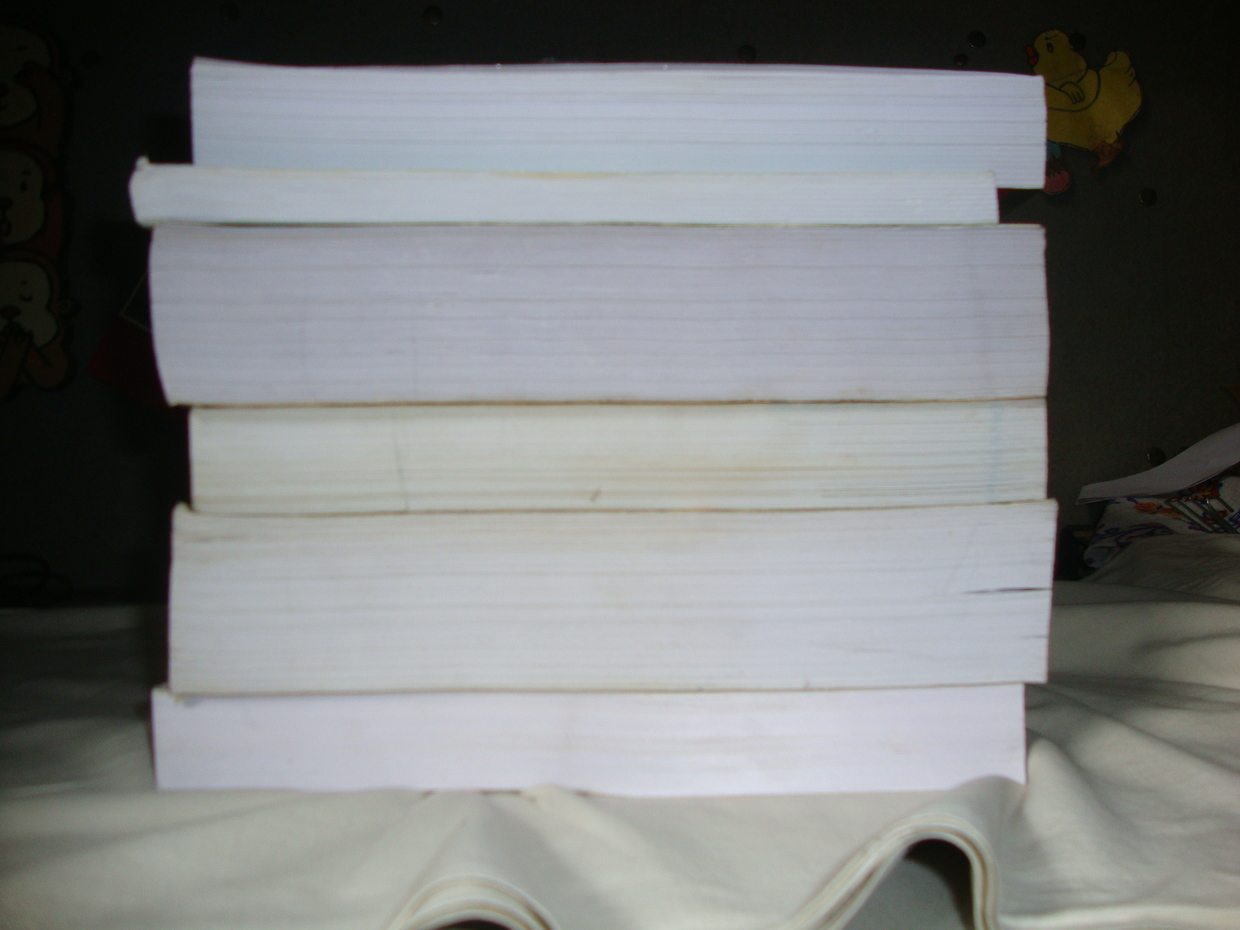
\includegraphics[width=1.0\linewidth,height=6.5in,keepaspectratio]{../images/9.jpg}
\end{center}
\raggedright{}\myfigurewithcaption{9}{Stack of books}
\end{minipage}\vspace{0.75cm}



Using stacks, we can solve many applications, some of which are listed below.









\subsubsection{Converting a decimal number into a binary number}
\label{43}
The logic for transforming a decimal number into a binary number is as follows:
\\

\TemplateSpaceIndent{$\text{ }${}$\text{ }${}$\text{ }${}$\text{ }${}$\text{ }${}*$\text{ }${}Read$\text{ }${}a$\text{ }${}number$\text{ }$\newline{}
$\text{ }${}$\text{ }${}$\text{ }${}$\text{ }${}$\text{ }${}*$\text{ }${}Iteration$\text{ }${}(while$\text{ }${}number$\text{ }${}is$\text{ }${}greater$\text{ }${}than$\text{ }${}zero)$\text{ }$\newline{}
$\text{ }${}$\text{ }${}$\text{ }${}$\text{ }${}$\text{ }${}$\text{ }${}$\text{ }${}$\text{ }${}$\text{ }${}$\text{ }${}$\text{ }${}$\text{ }${}$\text{ }${}$\text{ }${}$\text{ }${}1.$\text{ }${}Find$\text{ }${}out$\text{ }${}the$\text{ }${}remainder$\text{ }${}after$\text{ }${}dividing$\text{ }${}the$\text{ }${}number$\text{ }${}by$\text{ }${}2$\text{ }$\newline{}
$\text{ }${}$\text{ }${}$\text{ }${}$\text{ }${}$\text{ }${}$\text{ }${}$\text{ }${}$\text{ }${}$\text{ }${}$\text{ }${}$\text{ }${}$\text{ }${}$\text{ }${}$\text{ }${}$\text{ }${}2.$\text{ }${}Print$\text{ }${}the$\text{ }${}remainder$\text{ }$\newline{}
$\text{ }${}$\text{ }${}$\text{ }${}$\text{ }${}$\text{ }${}$\text{ }${}$\text{ }${}$\text{ }${}$\text{ }${}$\text{ }${}$\text{ }${}$\text{ }${}$\text{ }${}$\text{ }${}$\text{ }${}3.$\text{ }${}Divide$\text{ }${}the$\text{ }${}number$\text{ }${}by$\text{ }${}2$\text{ }$\newline{}
$\text{ }${}$\text{ }${}$\text{ }${}$\text{ }${}$\text{ }${}*$\text{ }${}End$\text{ }${}the$\text{ }${}iteration}


However, there is a problem with this logic. Suppose the number, whose binary form we want to find is 23. Using this logic, we get the result as 11101, instead of getting 10111.

To solve this problem, we use a stack. We make use of the {\itshape LIFO} \setmainfont[Path=/usr/share/fonts/truetype/cmu/,UprightFont=cmunrm.ttf,BoldFont=cmunbx.ttf,ItalicFont=cmunti.ttf,BoldItalicFont=cmunbi.ttf]{cmunrm.ttf}\setmonofont[Path=/usr/share/fonts/truetype/cmu/,UprightFont=cmuntt.ttf,BoldFont=cmuntb.ttf,ItalicFont=cmunit.ttf,BoldItalicFont=cmuntx.ttf]{cmunrm.ttf} property of the stack. Initially we {\itshape push} \setmainfont[Path=/usr/share/fonts/truetype/cmu/,UprightFont=cmunrm.ttf,BoldFont=cmunbx.ttf,ItalicFont=cmunti.ttf,BoldItalicFont=cmunbi.ttf]{cmunrm.ttf}\setmonofont[Path=/usr/share/fonts/truetype/cmu/,UprightFont=cmuntt.ttf,BoldFont=cmuntb.ttf,ItalicFont=cmunit.ttf,BoldItalicFont=cmuntx.ttf]{cmunrm.ttf} the binary digit formed into the stack, instead of printing it directly. After the entire digit has been converted into the binary form, we {\itshape pop} \setmainfont[Path=/usr/share/fonts/truetype/cmu/,UprightFont=cmunrm.ttf,BoldFont=cmunbx.ttf,ItalicFont=cmunti.ttf,BoldItalicFont=cmunbi.ttf]{cmunrm.ttf}\setmonofont[Path=/usr/share/fonts/truetype/cmu/,UprightFont=cmuntt.ttf,BoldFont=cmuntb.ttf,ItalicFont=cmunit.ttf,BoldItalicFont=cmuntx.ttf]{cmunrm.ttf} one digit at a time from the stack and print it. Therefore we get the decimal number is converted into its proper binary form.

{\bfseries \setmainfont[Path=/usr/share/fonts/truetype/cmu/,UprightFont=cmunrm.ttf,BoldFont=cmunbx.ttf,ItalicFont=cmunti.ttf,BoldItalicFont=cmunbi.ttf]{cmunbx.ttf}\setmonofont[Path=/usr/share/fonts/truetype/cmu/,UprightFont=cmuntt.ttf,BoldFont=cmuntb.ttf,ItalicFont=cmunit.ttf,BoldItalicFont=cmuntx.ttf]{cmunbx.ttf}\bfseries Algorithm:} \setmainfont[Path=/usr/share/fonts/truetype/cmu/,UprightFont=cmunrm.ttf,BoldFont=cmunbx.ttf,ItalicFont=cmunti.ttf,BoldItalicFont=cmunbi.ttf]{cmunrm.ttf}\setmonofont[Path=/usr/share/fonts/truetype/cmu/,UprightFont=cmuntt.ttf,BoldFont=cmuntb.ttf,ItalicFont=cmunit.ttf,BoldItalicFont=cmuntx.ttf]{cmunrm.ttf}
\\

\TemplateSpaceIndent{$\text{ }${}$\text{ }${}$\text{ }${}$\text{ }${}1.$\text{ }${}Create$\text{ }${}a$\text{ }${}stack$\text{ }$\newline{}
$\text{ }${}$\text{ }${}$\text{ }${}$\text{ }${}2.$\text{ }${}Enter$\text{ }${}a$\text{ }${}decimal$\text{ }${}number,$\text{ }${}which$\text{ }${}has$\text{ }${}to$\text{ }${}be$\text{ }${}converted$\text{ }${}into$\text{ }${}its$\text{ }${}equivalent$\text{ }$\newline{}
$\text{ }${}binary$\text{ }${}form.$\text{ }$\newline{}
$\text{ }${}$\text{ }${}$\text{ }${}$\text{ }${}3.$\text{ }${}iteration1$\text{ }${}(while$\text{ }${}number$\text{ }${}>{}$\text{ }${}0)$\text{ }$\newline{}
$\text{ }${}$\text{ }${}$\text{ }${}$\text{ }${}$\text{ }${}$\text{ }${}$\text{ }${}$\text{ }${}$\text{ }${}$\text{ }${}3.1$\text{ }${}digit$\text{ }${}=$\text{ }${}number$\text{ }${}\%$\text{ }${}2$\text{ }$\newline{}
$\text{ }${}$\text{ }${}$\text{ }${}$\text{ }${}$\text{ }${}$\text{ }${}$\text{ }${}$\text{ }${}$\text{ }${}$\text{ }${}3.2$\text{ }${}Push$\text{ }${}{\itshape digit} $\text{ }${}\setmainfont[Path=/usr/share/fonts/truetype/cmu/,UprightFont=cmunrm.ttf,BoldFont=cmunbx.ttf,ItalicFont=cmunti.ttf,BoldItalicFont=cmunbi.ttf]{cmunrm.ttf}\setmonofont[Path=/usr/share/fonts/truetype/cmu/,UprightFont=cmuntt.ttf,BoldFont=cmuntb.ttf,ItalicFont=cmunit.ttf,BoldItalicFont=cmuntx.ttf]{cmunrm.ttf}into$\text{ }${}the$\text{ }${}stack$\text{ }$\newline{}
$\text{ }${}$\text{ }${}$\text{ }${}$\text{ }${}$\text{ }${}$\text{ }${}$\text{ }${}$\text{ }${}$\text{ }${}$\text{ }${}3.3$\text{ }${}If$\text{ }${}the$\text{ }${}stack$\text{ }${}is$\text{ }${}full$\text{ }$\newline{}
$\text{ }${}$\text{ }${}$\text{ }${}$\text{ }${}$\text{ }${}$\text{ }${}$\text{ }${}$\text{ }${}$\text{ }${}$\text{ }${}$\text{ }${}$\text{ }${}$\text{ }${}$\text{ }${}$\text{ }${}3.3.1$\text{ }${}Print$\text{ }${}an$\text{ }${}error$\text{ }$\newline{}
$\text{ }${}$\text{ }${}$\text{ }${}$\text{ }${}$\text{ }${}$\text{ }${}$\text{ }${}$\text{ }${}$\text{ }${}$\text{ }${}$\text{ }${}$\text{ }${}$\text{ }${}$\text{ }${}$\text{ }${}3.3.2$\text{ }${}Stop$\text{ }${}the$\text{ }${}algorithm$\text{ }$\newline{}
$\text{ }${}$\text{ }${}$\text{ }${}$\text{ }${}$\text{ }${}$\text{ }${}$\text{ }${}$\text{ }${}$\text{ }${}$\text{ }${}3.4$\text{ }${}End$\text{ }${}the$\text{ }${}{\itshape if} $\text{ }${}\setmainfont[Path=/usr/share/fonts/truetype/cmu/,UprightFont=cmunrm.ttf,BoldFont=cmunbx.ttf,ItalicFont=cmunti.ttf,BoldItalicFont=cmunbi.ttf]{cmunrm.ttf}\setmonofont[Path=/usr/share/fonts/truetype/cmu/,UprightFont=cmuntt.ttf,BoldFont=cmuntb.ttf,ItalicFont=cmunit.ttf,BoldItalicFont=cmuntx.ttf]{cmunrm.ttf}condition$\text{ }$\newline{}
$\text{ }${}$\text{ }${}$\text{ }${}$\text{ }${}$\text{ }${}$\text{ }${}$\text{ }${}$\text{ }${}$\text{ }${}$\text{ }${}3.5$\text{ }${}Divide$\text{ }${}the$\text{ }${}number$\text{ }${}by$\text{ }${}2$\text{ }$\newline{}
$\text{ }${}$\text{ }${}$\text{ }${}$\text{ }${}4.$\text{ }${}End$\text{ }${}{\itshape iteration1} $\text{ }$\newline{}
$\text{ }${}$\text{ }${}$\text{ }${}$\text{ }${}$\text{ }$\newline{}
$\text{ }${}$\text{ }${}$\text{ }${}$\text{ }${}\setmainfont[Path=/usr/share/fonts/truetype/cmu/,UprightFont=cmunrm.ttf,BoldFont=cmunbx.ttf,ItalicFont=cmunti.ttf,BoldItalicFont=cmunbi.ttf]{cmunrm.ttf}\setmonofont[Path=/usr/share/fonts/truetype/cmu/,UprightFont=cmuntt.ttf,BoldFont=cmuntb.ttf,ItalicFont=cmunit.ttf,BoldItalicFont=cmuntx.ttf]{cmunrm.ttf}5.$\text{ }${}iteration2$\text{ }${}(while$\text{ }${}stack$\text{ }${}is$\text{ }${}not$\text{ }${}empty)$\text{ }$\newline{}
$\text{ }${}$\text{ }${}$\text{ }${}$\text{ }${}$\text{ }${}$\text{ }${}$\text{ }${}$\text{ }${}$\text{ }${}$\text{ }${}5.1$\text{ }${}Pop$\text{ }${}{\itshape digit} $\text{ }${}\setmainfont[Path=/usr/share/fonts/truetype/cmu/,UprightFont=cmunrm.ttf,BoldFont=cmunbx.ttf,ItalicFont=cmunti.ttf,BoldItalicFont=cmunbi.ttf]{cmunrm.ttf}\setmonofont[Path=/usr/share/fonts/truetype/cmu/,UprightFont=cmuntt.ttf,BoldFont=cmuntb.ttf,ItalicFont=cmunit.ttf,BoldItalicFont=cmuntx.ttf]{cmunrm.ttf}from$\text{ }${}the$\text{ }${}stack$\text{ }$\newline{}
$\text{ }${}$\text{ }${}$\text{ }${}$\text{ }${}$\text{ }${}$\text{ }${}$\text{ }${}$\text{ }${}$\text{ }${}$\text{ }${}5.2$\text{ }${}Print$\text{ }${}the$\text{ }${}{\itshape digit} $\text{ }$\newline{}
$\text{ }${}$\text{ }${}$\text{ }${}$\text{ }${}\setmainfont[Path=/usr/share/fonts/truetype/cmu/,UprightFont=cmunrm.ttf,BoldFont=cmunbx.ttf,ItalicFont=cmunti.ttf,BoldItalicFont=cmunbi.ttf]{cmunrm.ttf}\setmonofont[Path=/usr/share/fonts/truetype/cmu/,UprightFont=cmuntt.ttf,BoldFont=cmuntb.ttf,ItalicFont=cmunit.ttf,BoldItalicFont=cmuntx.ttf]{cmunrm.ttf}6.$\text{ }${}End$\text{ }${}iteration2$\text{ }$\newline{}
$\text{ }${}$\text{ }${}$\text{ }${}$\text{ }${}7.$\text{ }${}STOP}

\subsubsection{Towers of Hanoi}
\label{44}


\begin{minipage}{0.75000\textwidth}
\begin{center}
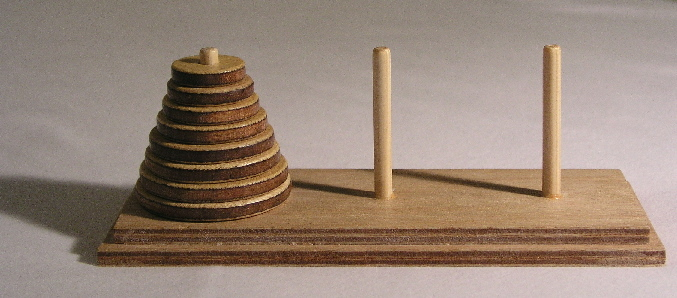
\includegraphics[width=1.0\textwidth,height=6.5in,keepaspectratio]{../images/10.jpg}
\end{center}
\raggedright{}\myfigurewithcaption{10}{Towers of Hanoi}
\end{minipage}\vspace{0.75cm}


One of the most interesting applications of stacks can be found in solving a puzzle called Tower of Hanoi. According to an old Brahmin story, the existence of the universe is calculated in terms of the time taken by a number of monks, who are working all the time, to move 64 disks from one pole to another. But there are some rules about how this should be done, which are:
\begin{myenumerate}
\item{}  You can move only one disk at a time.
\item{}  For temporary storage, a third pole may be used.
\item{}  You cannot place a disk of larger diameter on a disk of smaller diameter.\myfootnote{ How to Solve it by Computer. Prentice Hall of India, , 
}
\end{myenumerate}


Here we assume that  A is first tower, B is second tower  \& C is third tower. 



\begin{minipage}{0.93750\textwidth}
\begin{center}
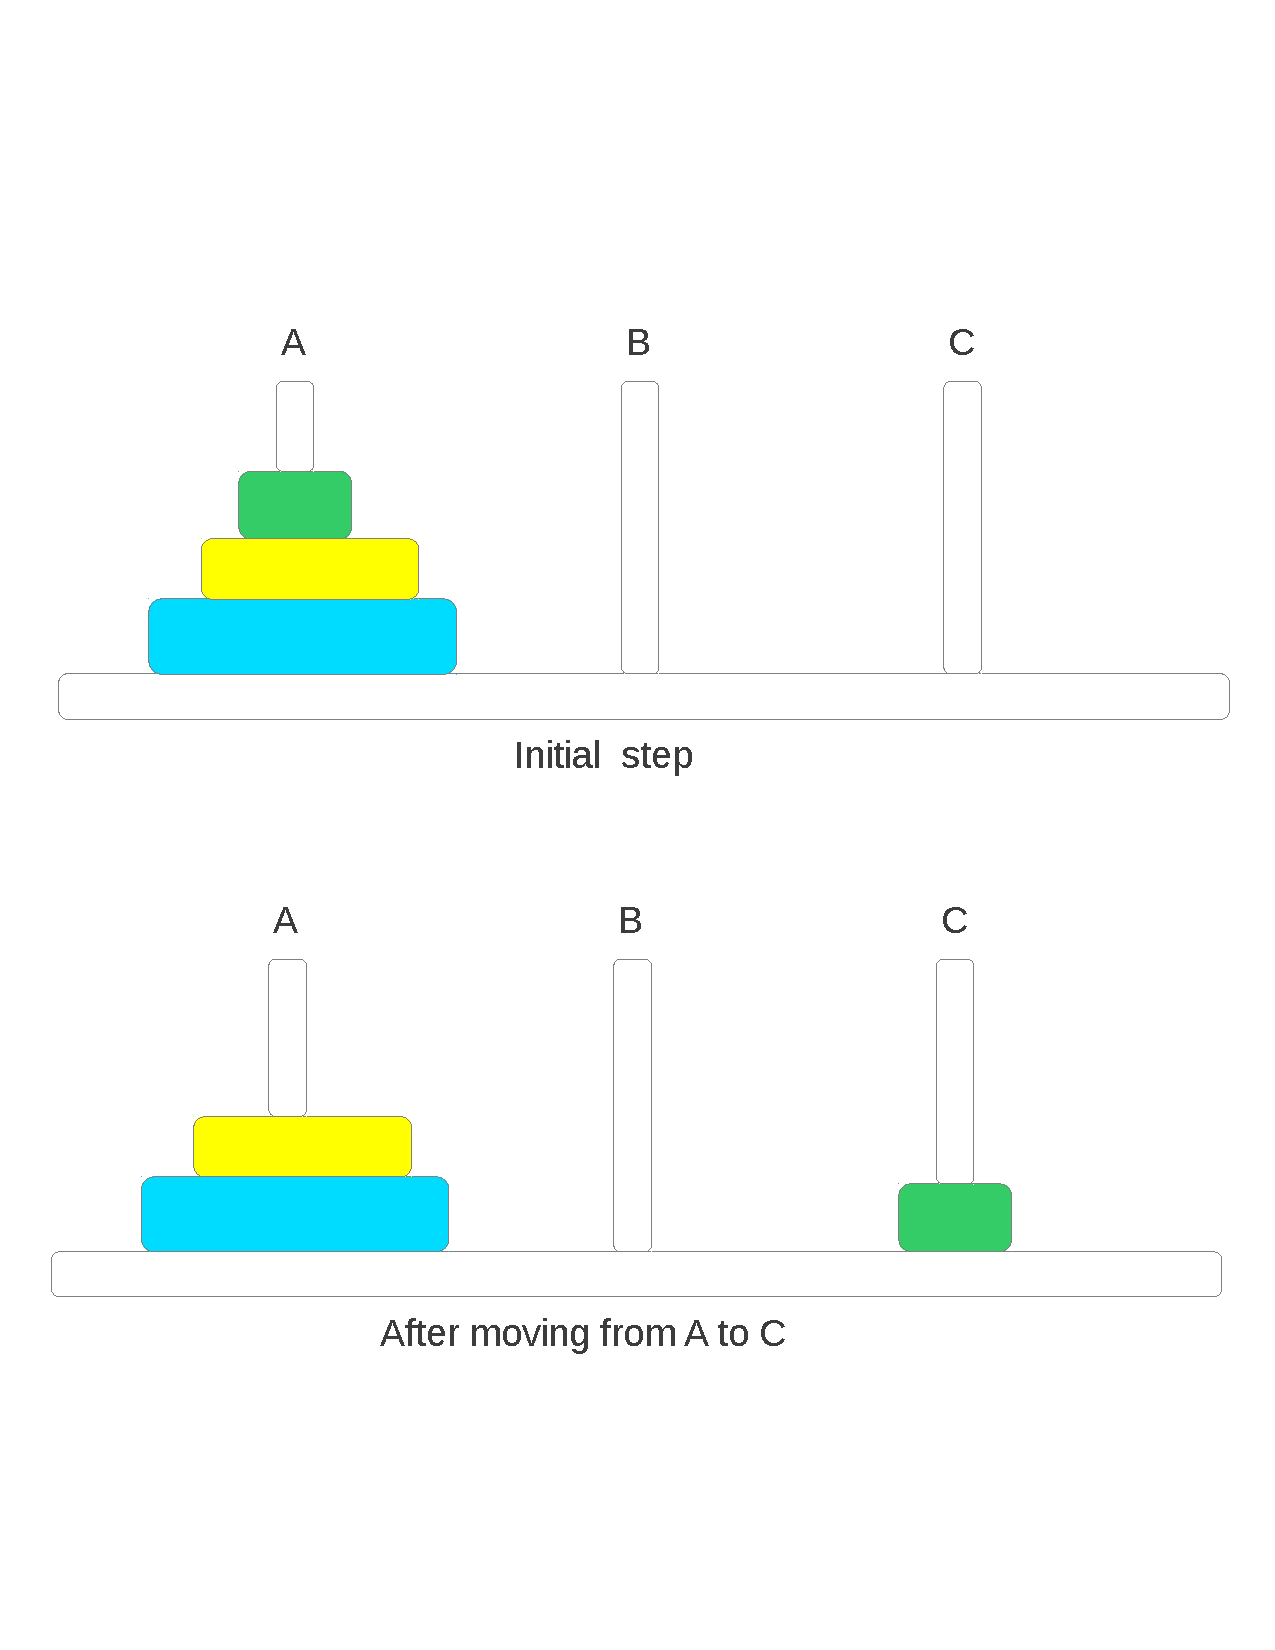
\includegraphics[width=1.0\textwidth,height=6.5in,keepaspectratio]{../images/11.pdf}
\end{center}
\raggedright{}\myfigurewithcaption{11}{Towers of Hanoi step 1}
\end{minipage}\vspace{0.75cm}





\begin{minipage}{0.93750\textwidth}
\begin{center}
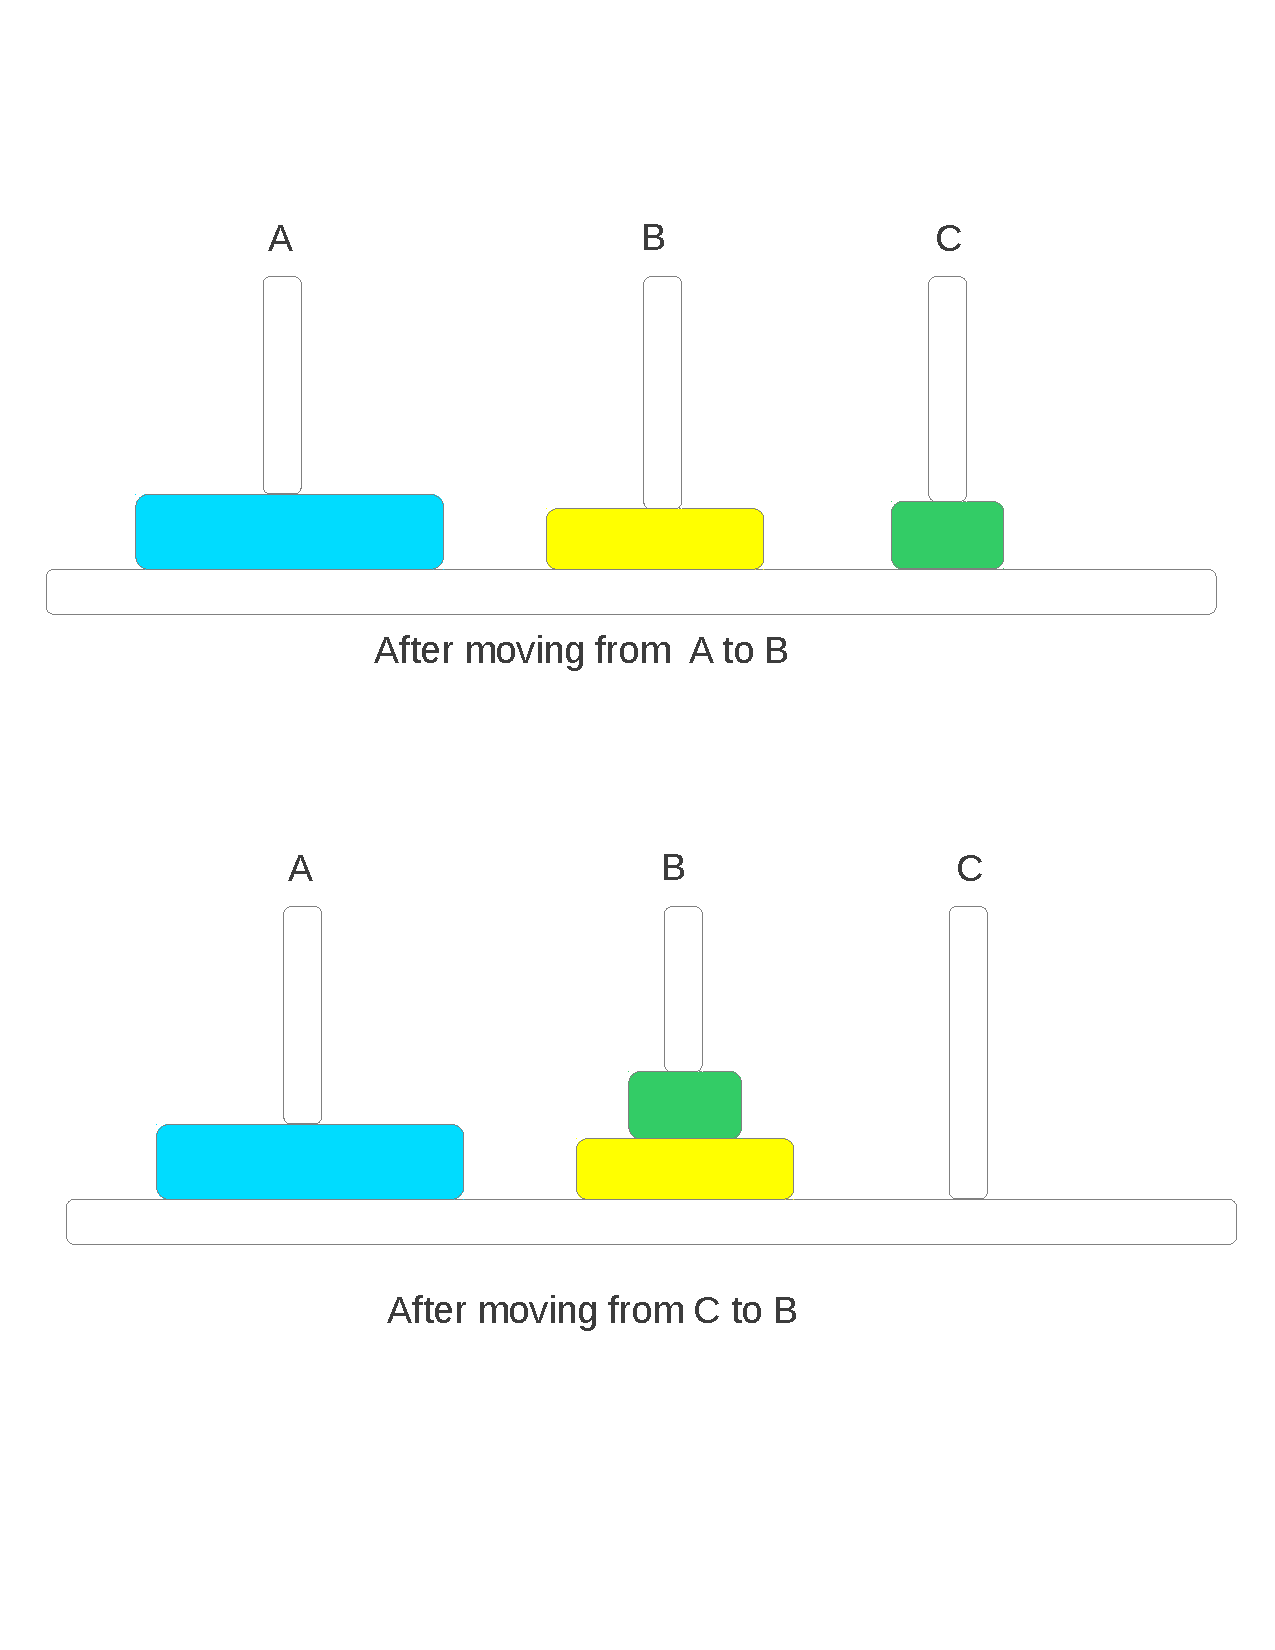
\includegraphics[width=1.0\textwidth,height=6.5in,keepaspectratio]{../images/12.pdf}
\end{center}
\raggedright{}\myfigurewithcaption{12}{Towers of Hanoi step 2}
\end{minipage}\vspace{0.75cm}

 



\begin{minipage}{0.93750\textwidth}
\begin{center}
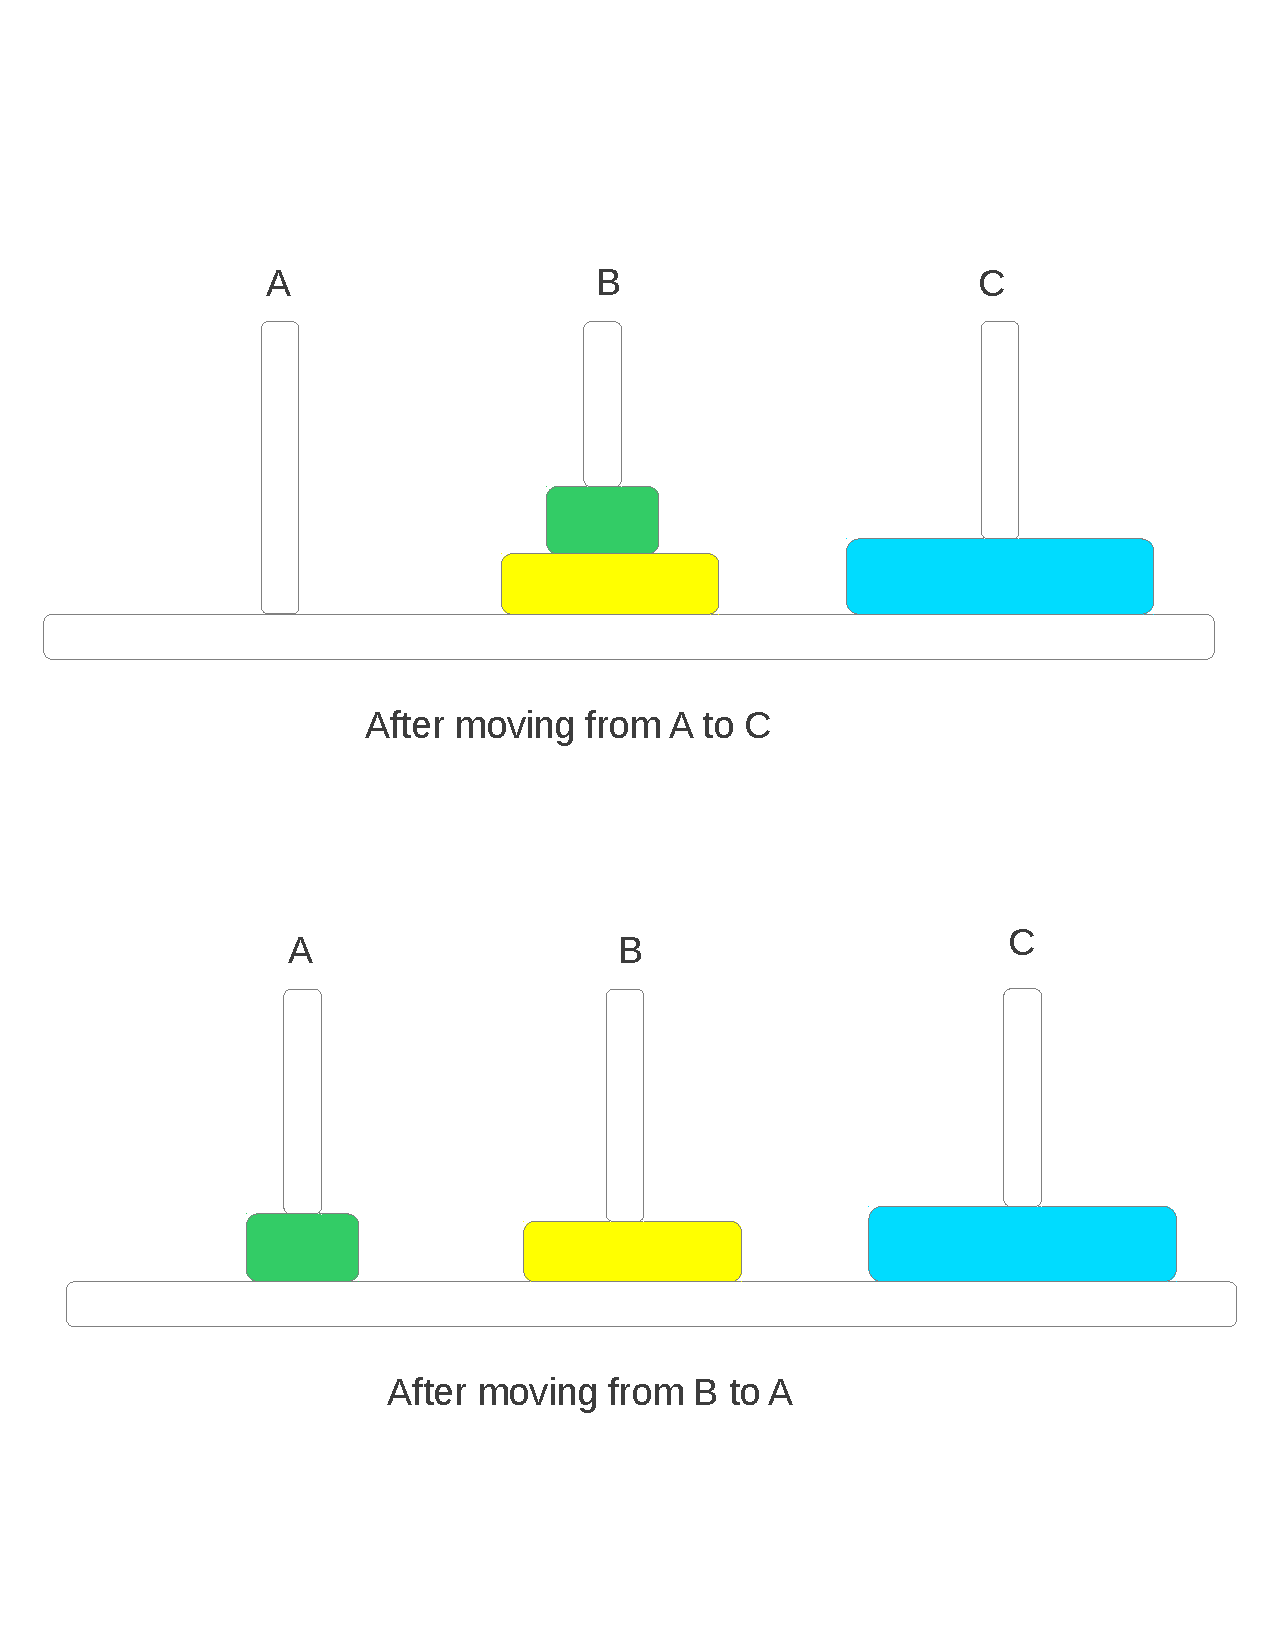
\includegraphics[width=1.0\textwidth,height=6.5in,keepaspectratio]{../images/13.pdf}
\end{center}
\raggedright{}\myfigurewithcaption{13}{Towers of Hanoi step 3}
\end{minipage}\vspace{0.75cm}

 




\begin{minipage}{0.93750\textwidth}
\begin{center}
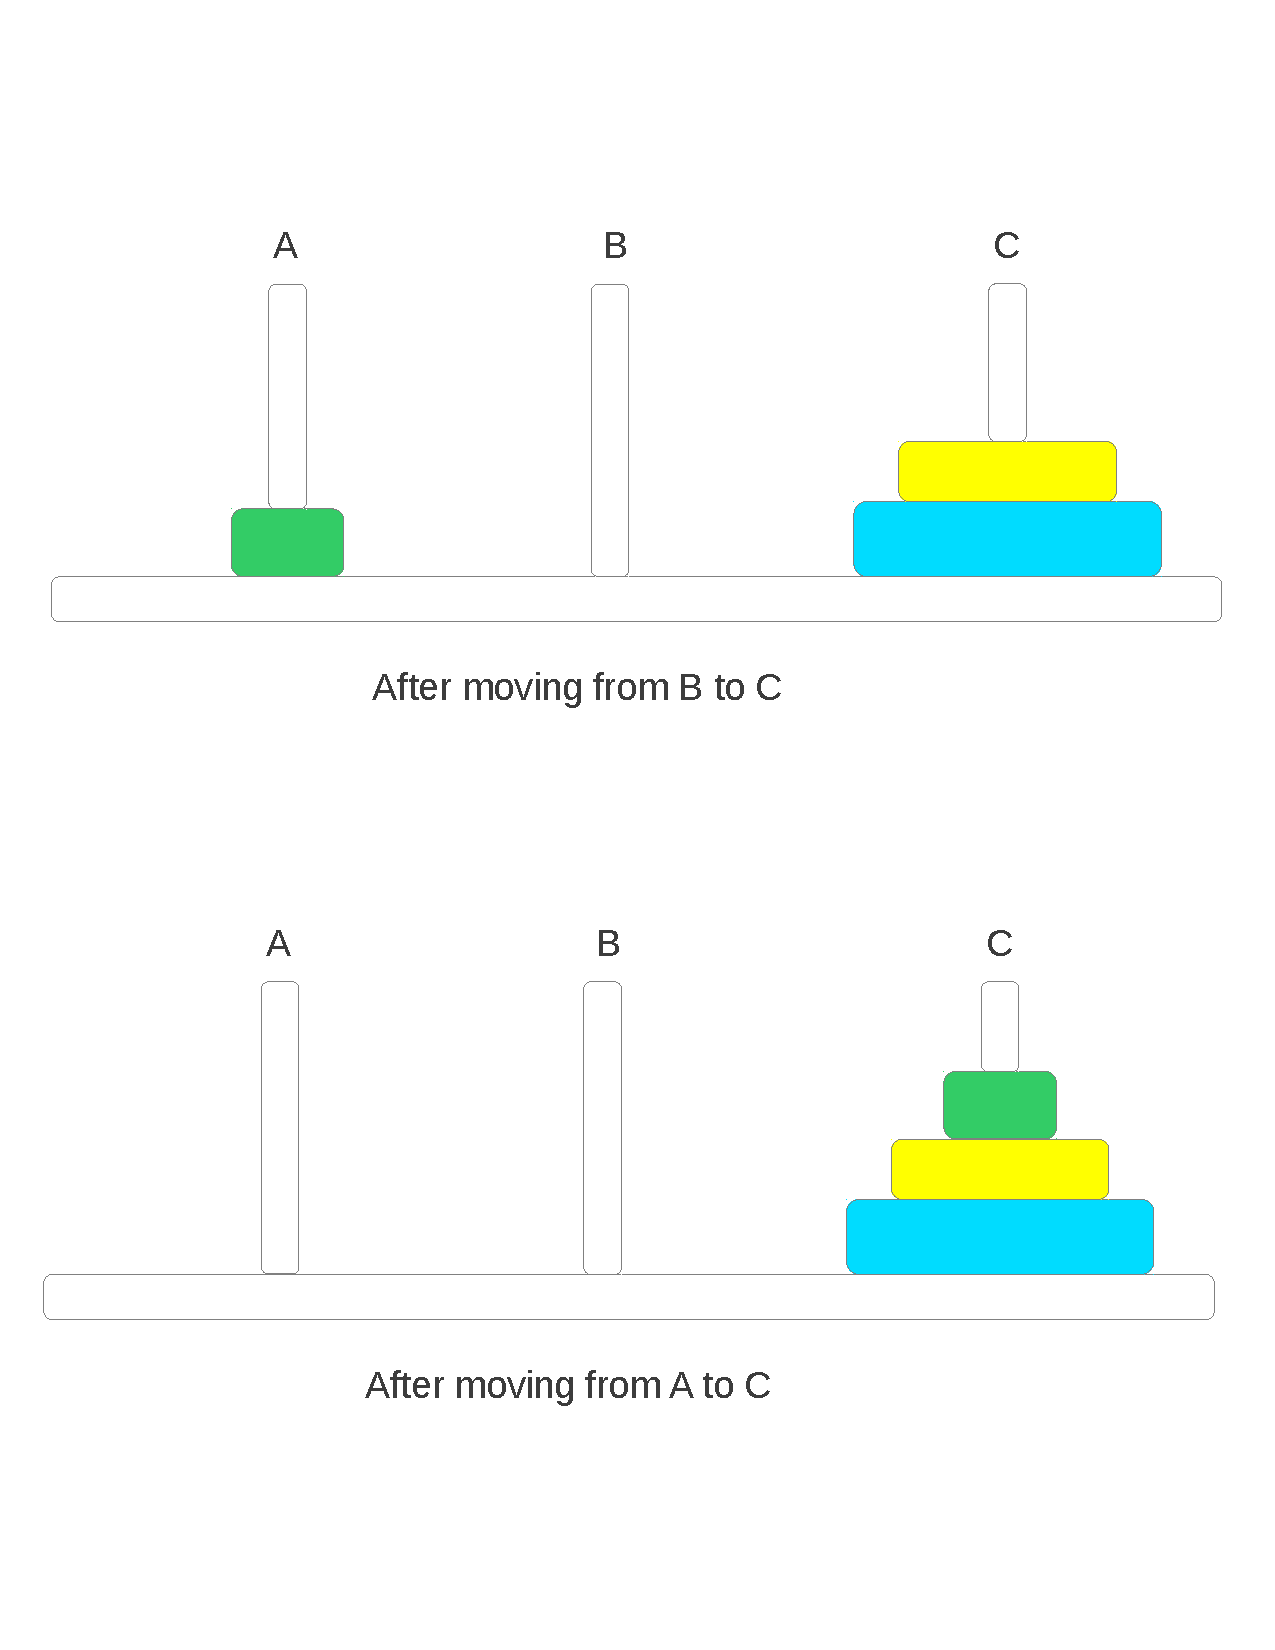
\includegraphics[width=1.0\textwidth,height=6.5in,keepaspectratio]{../images/14.pdf}
\end{center}
\raggedright{}\myfigurewithcaption{14}{Towers of Hanoi step 4}
\end{minipage}\vspace{0.75cm}






\begin{minipage}{0.87500\textwidth}
\begin{center}
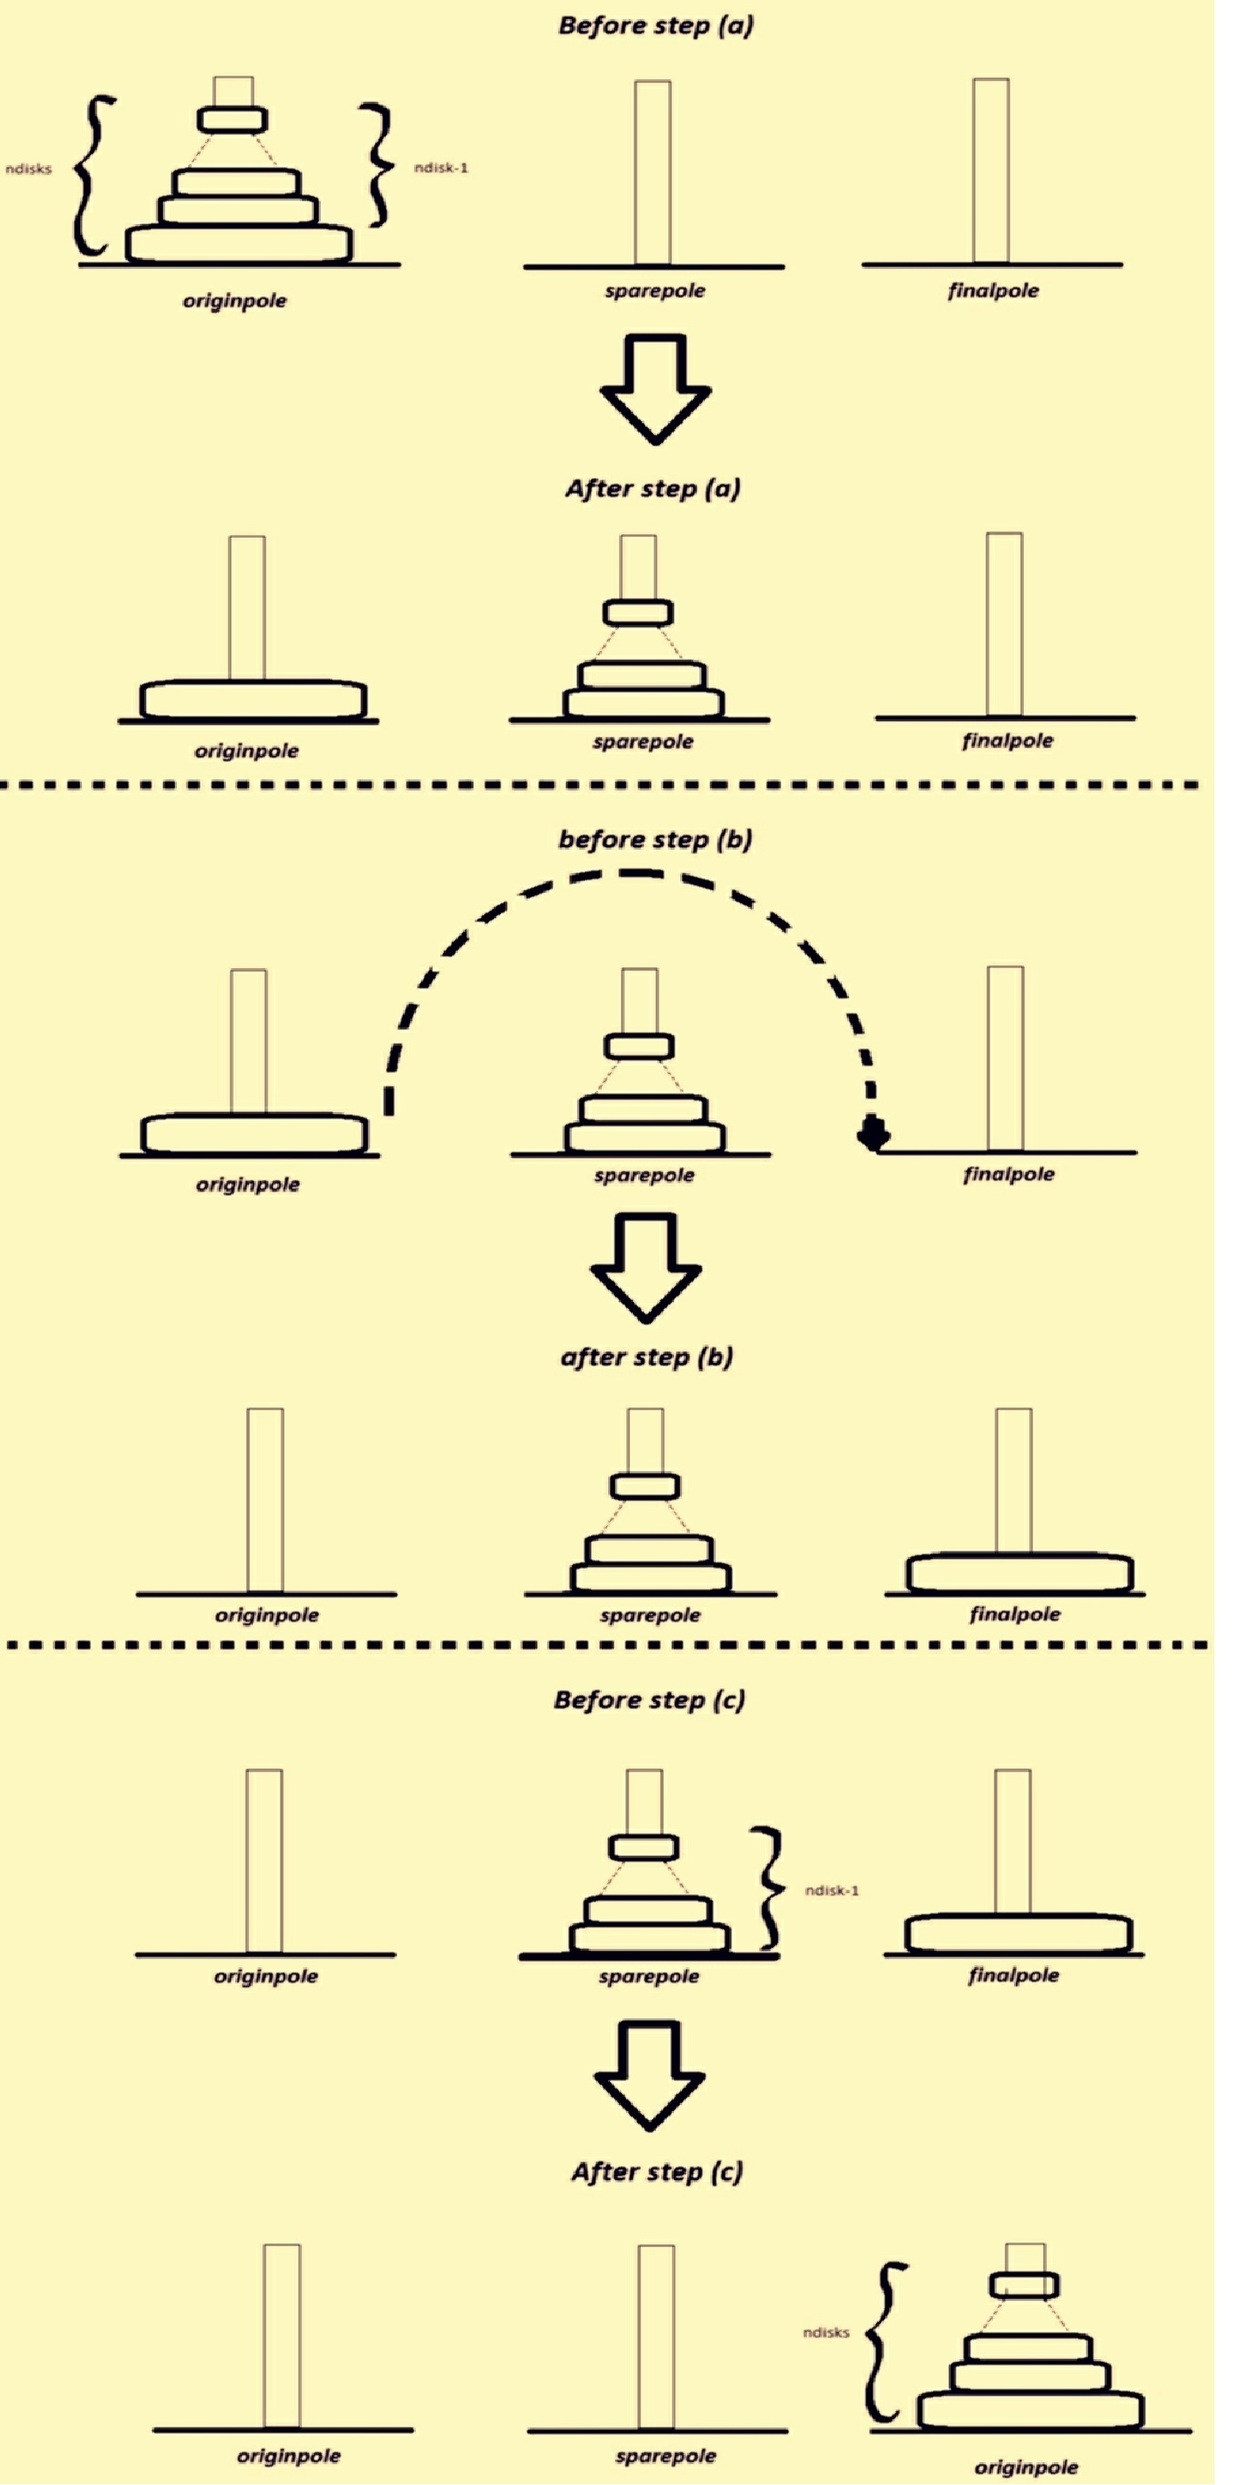
\includegraphics[width=1.0\textwidth,height=6.5in,keepaspectratio]{../images/15.jpg}
\end{center}
\raggedright{}\myfigurewithcaption{15}{Tower of Hanoi}
\end{minipage}\vspace{0.75cm}



{\bfseries \setmainfont[Path=/usr/share/fonts/truetype/cmu/,UprightFont=cmunrm.ttf,BoldFont=cmunbx.ttf,ItalicFont=cmunti.ttf,BoldItalicFont=cmunbi.ttf]{cmunbx.ttf}\setmonofont[Path=/usr/share/fonts/truetype/cmu/,UprightFont=cmuntt.ttf,BoldFont=cmuntb.ttf,ItalicFont=cmunit.ttf,BoldItalicFont=cmuntx.ttf]{cmunbx.ttf}\bfseries Output : (when there are 3 disks)} \setmainfont[Path=/usr/share/fonts/truetype/cmu/,UprightFont=cmunrm.ttf,BoldFont=cmunbx.ttf,ItalicFont=cmunti.ttf,BoldItalicFont=cmunbi.ttf]{cmunrm.ttf}\setmonofont[Path=/usr/share/fonts/truetype/cmu/,UprightFont=cmuntt.ttf,BoldFont=cmuntb.ttf,ItalicFont=cmunit.ttf,BoldItalicFont=cmuntx.ttf]{cmunrm.ttf}

Let {\itshape 1} \setmainfont[Path=/usr/share/fonts/truetype/cmu/,UprightFont=cmunrm.ttf,BoldFont=cmunbx.ttf,ItalicFont=cmunti.ttf,BoldItalicFont=cmunbi.ttf]{cmunrm.ttf}\setmonofont[Path=/usr/share/fonts/truetype/cmu/,UprightFont=cmuntt.ttf,BoldFont=cmuntb.ttf,ItalicFont=cmunit.ttf,BoldItalicFont=cmuntx.ttf]{cmunrm.ttf} be the smallest disk, {\itshape 2} \setmainfont[Path=/usr/share/fonts/truetype/cmu/,UprightFont=cmunrm.ttf,BoldFont=cmunbx.ttf,ItalicFont=cmunti.ttf,BoldItalicFont=cmunbi.ttf]{cmunrm.ttf}\setmonofont[Path=/usr/share/fonts/truetype/cmu/,UprightFont=cmuntt.ttf,BoldFont=cmuntb.ttf,ItalicFont=cmunit.ttf,BoldItalicFont=cmuntx.ttf]{cmunrm.ttf} be the disk of medium size and {\itshape 3} \setmainfont[Path=/usr/share/fonts/truetype/cmu/,UprightFont=cmunrm.ttf,BoldFont=cmunbx.ttf,ItalicFont=cmunti.ttf,BoldItalicFont=cmunbi.ttf]{cmunrm.ttf}\setmonofont[Path=/usr/share/fonts/truetype/cmu/,UprightFont=cmuntt.ttf,BoldFont=cmuntb.ttf,ItalicFont=cmunit.ttf,BoldItalicFont=cmuntx.ttf]{cmunrm.ttf} be the largest disk.
\begin{longtable}{|>{\RaggedRight}p{0.34177\linewidth}|>{\RaggedRight}p{0.32494\linewidth}|>{\RaggedRight}p{0.24758\linewidth}|} \hline 
{\bfseries \hspace*{0pt}\ignorespaces{}\hspace*{0pt} Move disk}&{\bfseries \hspace*{0pt}\ignorespaces{}\hspace*{0pt} From peg }&{\bfseries \hspace*{0pt}\ignorespaces{}\hspace*{0pt} To peg }\endhead  \hline \hspace*{0pt}\ignorespaces{}\hspace*{0pt} 1&\hspace*{0pt}\ignorespaces{}\hspace*{0pt} A&\hspace*{0pt}\ignorespaces{}\hspace*{0pt} C\\ \hline \hspace*{0pt}\ignorespaces{}\hspace*{0pt} 2&\hspace*{0pt}\ignorespaces{}\hspace*{0pt} A&\hspace*{0pt}\ignorespaces{}\hspace*{0pt} B\\ \hline \hspace*{0pt}\ignorespaces{}\hspace*{0pt} 1&\hspace*{0pt}\ignorespaces{}\hspace*{0pt} C&\hspace*{0pt}\ignorespaces{}\hspace*{0pt} B\\ \hline \hspace*{0pt}\ignorespaces{}\hspace*{0pt} 3&\hspace*{0pt}\ignorespaces{}\hspace*{0pt} A&\hspace*{0pt}\ignorespaces{}\hspace*{0pt} C\\ \hline \hspace*{0pt}\ignorespaces{}\hspace*{0pt} 1&\hspace*{0pt}\ignorespaces{}\hspace*{0pt} B&\hspace*{0pt}\ignorespaces{}\hspace*{0pt} A\\ \hline \hspace*{0pt}\ignorespaces{}\hspace*{0pt} 2&\hspace*{0pt}\ignorespaces{}\hspace*{0pt} B&\hspace*{0pt}\ignorespaces{}\hspace*{0pt} C\\ \hline \hspace*{0pt}\ignorespaces{}\hspace*{0pt} 1&\hspace*{0pt}\ignorespaces{}\hspace*{0pt} A&\hspace*{0pt}\ignorespaces{}\hspace*{0pt} C\\ \hline 
\end{longtable}


{\bfseries \setmainfont[Path=/usr/share/fonts/truetype/cmu/,UprightFont=cmunrm.ttf,BoldFont=cmunbx.ttf,ItalicFont=cmunti.ttf,BoldItalicFont=cmunbi.ttf]{cmunbx.ttf}\setmonofont[Path=/usr/share/fonts/truetype/cmu/,UprightFont=cmuntt.ttf,BoldFont=cmuntb.ttf,ItalicFont=cmunit.ttf,BoldItalicFont=cmuntx.ttf]{cmunbx.ttf}\bfseries Output : (when there are 4 disks)} 
\begin{longtable}{|>{\RaggedRight}p{0.33905\linewidth}|>{\RaggedRight}p{0.32291\linewidth}|>{\RaggedRight}p{0.25232\linewidth}|} \hline 
{\bfseries \hspace*{0pt}\ignorespaces{}\hspace*{0pt}\setmainfont[Path=/usr/share/fonts/truetype/cmu/,UprightFont=cmunrm.ttf,BoldFont=cmunbx.ttf,ItalicFont=cmunti.ttf,BoldItalicFont=cmunbi.ttf]{cmunrm.ttf}\setmonofont[Path=/usr/share/fonts/truetype/cmu/,UprightFont=cmuntt.ttf,BoldFont=cmuntb.ttf,ItalicFont=cmunit.ttf,BoldItalicFont=cmuntx.ttf]{cmunrm.ttf} Move disk}&{\bfseries \hspace*{0pt}\ignorespaces{}\hspace*{0pt} From peg }&{\bfseries \hspace*{0pt}\ignorespaces{}\hspace*{0pt} To peg }\endhead  \hline \hspace*{0pt}\ignorespaces{}\hspace*{0pt} 1&\hspace*{0pt}\ignorespaces{}\hspace*{0pt} A&\hspace*{0pt}\ignorespaces{}\hspace*{0pt} B\\ \hline \hspace*{0pt}\ignorespaces{}\hspace*{0pt} 2&\hspace*{0pt}\ignorespaces{}\hspace*{0pt} A&\hspace*{0pt}\ignorespaces{}\hspace*{0pt} C\\ \hline \hspace*{0pt}\ignorespaces{}\hspace*{0pt} 1&\hspace*{0pt}\ignorespaces{}\hspace*{0pt} B&\hspace*{0pt}\ignorespaces{}\hspace*{0pt} C\\ \hline \hspace*{0pt}\ignorespaces{}\hspace*{0pt} 3&\hspace*{0pt}\ignorespaces{}\hspace*{0pt} A&\hspace*{0pt}\ignorespaces{}\hspace*{0pt} B\\ \hline \hspace*{0pt}\ignorespaces{}\hspace*{0pt} 1&\hspace*{0pt}\ignorespaces{}\hspace*{0pt} C&\hspace*{0pt}\ignorespaces{}\hspace*{0pt} A\\ \hline \hspace*{0pt}\ignorespaces{}\hspace*{0pt} 2&\hspace*{0pt}\ignorespaces{}\hspace*{0pt} C&\hspace*{0pt}\ignorespaces{}\hspace*{0pt} B\\ \hline \hspace*{0pt}\ignorespaces{}\hspace*{0pt} 1&\hspace*{0pt}\ignorespaces{}\hspace*{0pt} A&\hspace*{0pt}\ignorespaces{}\hspace*{0pt} B\\ \hline \hspace*{0pt}\ignorespaces{}\hspace*{0pt} 4&\hspace*{0pt}\ignorespaces{}\hspace*{0pt} A&\hspace*{0pt}\ignorespaces{}\hspace*{0pt} C\\ \hline \hspace*{0pt}\ignorespaces{}\hspace*{0pt} 1&\hspace*{0pt}\ignorespaces{}\hspace*{0pt} B&\hspace*{0pt}\ignorespaces{}\hspace*{0pt} C\\ \hline \hspace*{0pt}\ignorespaces{}\hspace*{0pt} 2&\hspace*{0pt}\ignorespaces{}\hspace*{0pt} B&\hspace*{0pt}\ignorespaces{}\hspace*{0pt} A\\ \hline \hspace*{0pt}\ignorespaces{}\hspace*{0pt} 1&\hspace*{0pt}\ignorespaces{}\hspace*{0pt} C&\hspace*{0pt}\ignorespaces{}\hspace*{0pt} A\\ \hline \hspace*{0pt}\ignorespaces{}\hspace*{0pt} 3&\hspace*{0pt}\ignorespaces{}\hspace*{0pt} B&\hspace*{0pt}\ignorespaces{}\hspace*{0pt} C\\ \hline \hspace*{0pt}\ignorespaces{}\hspace*{0pt} 1&\hspace*{0pt}\ignorespaces{}\hspace*{0pt} A&\hspace*{0pt}\ignorespaces{}\hspace*{0pt} B\\ \hline \hspace*{0pt}\ignorespaces{}\hspace*{0pt} 2&\hspace*{0pt}\ignorespaces{}\hspace*{0pt} A&\hspace*{0pt}\ignorespaces{}\hspace*{0pt} C\\ \hline \hspace*{0pt}\ignorespaces{}\hspace*{0pt} 1&\hspace*{0pt}\ignorespaces{}\hspace*{0pt} B&\hspace*{0pt}\ignorespaces{}\hspace*{0pt} C\\ \hline 
\end{longtable}


The C++ code for this solution can be implemented in two ways:
\paragraph{First Implementation (Without using Stacks)}
{$\text{ }$}\newline\label{45}
Here we assume that  A is first tower, B is second tower  \& C is third tower. (B is the intermediate)


\begin{Shaded}
\begin{Highlighting}[]

\DataTypeTok{void}\ensuremath{\text{ }}\NormalTok{TowersofHanoi(}\DataTypeTok{int}\ensuremath{\text{ }}\NormalTok{n,\ensuremath{\text{ }}}\DataTypeTok{int}\ensuremath{\text{ }}\NormalTok{a,\ensuremath{\text{ }}}\DataTypeTok{int}\ensuremath{\text{ }}\NormalTok{b,\ensuremath{\text{ }}}\DataTypeTok{int}\ensuremath{\text{ }}\NormalTok{c)}\newline
\NormalTok{\{}\newline
\ensuremath{\text{ }}\ensuremath{\text{ }}\ensuremath{\text{ }}\ensuremath{\text{ }}\CommentTok{//Move\ensuremath{\text{ }}top\ensuremath{\text{ }}n\ensuremath{\text{ }}disks\ensuremath{\text{ }}from\ensuremath{\text{ }}tower\ensuremath{\text{ }}a\ensuremath{\text{ }}to\ensuremath{\text{ }}tower\ensuremath{\text{ }}b,\ensuremath{\text{ }}use\ensuremath{\text{ }}tower\ensuremath{\text{ }}c\ensuremath{\text{ }}for\ensuremath{\text{ }}intermediate}\newline
\ensuremath{\text{ }}\NormalTok{storage.}\newline
\ensuremath{\text{ }}\ensuremath{\text{ }}\ensuremath{\text{ }}\ensuremath{\text{ }}\KeywordTok{if}\NormalTok{(n\ensuremath{\text{ }}>\ensuremath{\text{ }}}\DecValTok{0}\NormalTok{)}\newline
\ensuremath{\text{ }}\ensuremath{\text{ }}\ensuremath{\text{ }}\ensuremath{\text{ }}\NormalTok{\{}\newline
\ensuremath{\text{ }}\ensuremath{\text{ }}\ensuremath{\text{ }}\ensuremath{\text{ }}\ensuremath{\text{ }}\ensuremath{\text{ }}\ensuremath{\text{ }}\ensuremath{\text{ }}\NormalTok{TowersofHanoi(n}\DecValTok{-1}\NormalTok{,\ensuremath{\text{ }}a,\ensuremath{\text{ }}c,\ensuremath{\text{ }}b);\ensuremath{\text{ }}\ensuremath{\text{ }}\ensuremath{\text{ }}}\CommentTok{//recursion}\newline
\ensuremath{\text{ }}\ensuremath{\text{ }}\ensuremath{\text{ }}\ensuremath{\text{ }}\ensuremath{\text{ }}\ensuremath{\text{ }}\ensuremath{\text{ }}\ensuremath{\text{ }}\NormalTok{cout\ensuremath{\text{ }}<<\ensuremath{\text{ }}}\StringTok{"\ensuremath{\text{ }}Move\ensuremath{\text{ }}top\ensuremath{\text{ }}disk\ensuremath{\text{ }}from\ensuremath{\text{ }}tower\ensuremath{\text{ }}"}\ensuremath{\text{ }}\NormalTok{<<\ensuremath{\text{ }}a\ensuremath{\text{ }}<<\ensuremath{\text{ }}}\StringTok{"\ensuremath{\text{ }}to\ensuremath{\text{ }}tower\ensuremath{\text{ }}"}\ensuremath{\text{ }}\NormalTok{<<\ensuremath{\text{ }}b\ensuremath{\text{ }}<<\ensuremath{\text{ }}endl\ensuremath{\text{ }};}\newline
\ensuremath{\text{ }}\ensuremath{\text{ }}\ensuremath{\text{ }}\ensuremath{\text{ }}\ensuremath{\text{ }}\ensuremath{\text{ }}\ensuremath{\text{ }}\ensuremath{\text{ }}\CommentTok{//Move\ensuremath{\text{ }}n-1\ensuremath{\text{ }}disks\ensuremath{\text{ }}from\ensuremath{\text{ }}intermediate(b)\ensuremath{\text{ }}to\ensuremath{\text{ }}the\ensuremath{\text{ }}source(a)\ensuremath{\text{ }}back}\newline
\ensuremath{\text{ }}\ensuremath{\text{ }}\ensuremath{\text{ }}\ensuremath{\text{ }}\ensuremath{\text{ }}\ensuremath{\text{ }}\ensuremath{\text{ }}\ensuremath{\text{ }}\NormalTok{TowersofHanoi(n}\DecValTok{-1}\NormalTok{,\ensuremath{\text{ }}c,\ensuremath{\text{ }}b,\ensuremath{\text{ }}a);\ensuremath{\text{ }}\ensuremath{\text{ }}\ensuremath{\text{ }}}\CommentTok{//recursion}\newline
\ensuremath{\text{ }}\ensuremath{\text{ }}\ensuremath{\text{ }}\ensuremath{\text{ }}\NormalTok{\}}\newline
\NormalTok{\}}\newline
\end{Highlighting}
\end{Shaded}


\myfootnote{Data structures, Algorithms and Applications in C++ by Sartaj Sahni}
\paragraph{Second Implementation (Using Stacks)}
{$\text{ }$}\newline\label{46}

\begin{Shaded}
\begin{Highlighting}[]

\CommentTok{//\ensuremath{\text{ }}Global\ensuremath{\text{ }}variable\ensuremath{\text{ }},\ensuremath{\text{ }}tower\ensuremath{\text{ }}[1:3]\ensuremath{\text{ }}are\ensuremath{\text{ }}three\ensuremath{\text{ }}towers}\newline
\NormalTok{arrayStack<}\DataTypeTok{int}\NormalTok{>\ensuremath{\text{ }}tower[}\DecValTok{4}\NormalTok{];}\newline
\DataTypeTok{void}\ensuremath{\text{ }}\NormalTok{TowerofHanoi(}\DataTypeTok{int}\ensuremath{\text{ }}\NormalTok{n)}\newline
\NormalTok{\{}\newline
\ensuremath{\text{ }}\ensuremath{\text{ }}\ensuremath{\text{ }}\ensuremath{\text{ }}\CommentTok{//\ensuremath{\text{ }}Preprocessor\ensuremath{\text{ }}for\ensuremath{\text{ }}moveAndShow.}\newline
\ensuremath{\text{ }}\ensuremath{\text{ }}\ensuremath{\text{ }}\ensuremath{\text{ }}\KeywordTok{for}\ensuremath{\text{ }}\NormalTok{(}\DataTypeTok{int}\ensuremath{\text{ }}\NormalTok{d\ensuremath{\text{ }}=\ensuremath{\text{ }}n;\ensuremath{\text{ }}d\ensuremath{\text{ }}>\ensuremath{\text{ }}}\DecValTok{0}\NormalTok{;\ensuremath{\text{ }}d--)\ensuremath{\text{ }}\ensuremath{\text{ }}\ensuremath{\text{ }}\ensuremath{\text{ }}\ensuremath{\text{ }}\ensuremath{\text{ }}\ensuremath{\text{ }}\ensuremath{\text{ }}}\CommentTok{//initialize}\newline
\ensuremath{\text{ }}\ensuremath{\text{ }}\ensuremath{\text{ }}\ensuremath{\text{ }}\ensuremath{\text{ }}\ensuremath{\text{ }}\ensuremath{\text{ }}\ensuremath{\text{ }}\NormalTok{tower[}\DecValTok{1}\NormalTok{].push(d);\ensuremath{\text{ }}\ensuremath{\text{ }}\ensuremath{\text{ }}\ensuremath{\text{ }}\ensuremath{\text{ }}\ensuremath{\text{ }}\ensuremath{\text{ }}\ensuremath{\text{ }}\ensuremath{\text{ }}\ensuremath{\text{ }}\ensuremath{\text{ }}\ensuremath{\text{ }}\ensuremath{\text{ }}\ensuremath{\text{ }}}\CommentTok{//add\ensuremath{\text{ }}disk\ensuremath{\text{ }}d\ensuremath{\text{ }}to\ensuremath{\text{ }}tower\ensuremath{\text{ }}1}\newline
\ensuremath{\text{ }}\ensuremath{\text{ }}\ensuremath{\text{ }}\ensuremath{\text{ }}\NormalTok{moveAndShow(n,\ensuremath{\text{ }}}\DecValTok{1}\NormalTok{,\ensuremath{\text{ }}}\DecValTok{2}\NormalTok{,\ensuremath{\text{ }}}\DecValTok{3}\NormalTok{);\ensuremath{\text{ }}\ensuremath{\text{ }}\ensuremath{\text{ }}\ensuremath{\text{ }}\ensuremath{\text{ }}\ensuremath{\text{ }}\ensuremath{\text{ }}\ensuremath{\text{ }}\ensuremath{\text{ }}\ensuremath{\text{ }}\ensuremath{\text{ }}}\CommentTok{/*move\ensuremath{\text{ }}n\ensuremath{\text{ }}disks\ensuremath{\text{ }}from\ensuremath{\text{ }}tower\ensuremath{\text{ }}1\ensuremath{\text{ }}to\ensuremath{\text{ }}tower\ensuremath{\text{ }}3}\newline
\CommentTok{\ensuremath{\text{ }}using\ensuremath{\text{ }}}\newline
\CommentTok{\ensuremath{\text{ }}\ensuremath{\text{ }}\ensuremath{\text{ }}\ensuremath{\text{ }}\ensuremath{\text{ }}\ensuremath{\text{ }}\ensuremath{\text{ }}\ensuremath{\text{ }}\ensuremath{\text{ }}\ensuremath{\text{ }}\ensuremath{\text{ }}\ensuremath{\text{ }}\ensuremath{\text{ }}\ensuremath{\text{ }}\ensuremath{\text{ }}\ensuremath{\text{ }}\ensuremath{\text{ }}\ensuremath{\text{ }}\ensuremath{\text{ }}\ensuremath{\text{ }}\ensuremath{\text{ }}\ensuremath{\text{ }}\ensuremath{\text{ }}\ensuremath{\text{ }}\ensuremath{\text{ }}\ensuremath{\text{ }}\ensuremath{\text{ }}\ensuremath{\text{ }}\ensuremath{\text{ }}\ensuremath{\text{ }}\ensuremath{\text{ }}\ensuremath{\text{ }}\ensuremath{\text{ }}\ensuremath{\text{ }}\ensuremath{\text{ }}\ensuremath{\text{ }}\ensuremath{\text{ }}\ensuremath{\text{ }}\ensuremath{\text{ }}tower\ensuremath{\text{ }}2\ensuremath{\text{ }}as\ensuremath{\text{ }}intermediate\ensuremath{\text{ }}tower*/}\ensuremath{\text{ }}\ensuremath{\text{ }}\newline
\NormalTok{\}}\newline
\ensuremath{\text{ }}\newline
\DataTypeTok{void}\ensuremath{\text{ }}\NormalTok{moveAndShow(}\DataTypeTok{int}\ensuremath{\text{ }}\NormalTok{n,\ensuremath{\text{ }}}\DataTypeTok{int}\ensuremath{\text{ }}\NormalTok{a,\ensuremath{\text{ }}}\DataTypeTok{int}\ensuremath{\text{ }}\NormalTok{b,\ensuremath{\text{ }}}\DataTypeTok{int}\ensuremath{\text{ }}\NormalTok{c)}\newline
\NormalTok{\{}\newline
\ensuremath{\text{ }}\ensuremath{\text{ }}\ensuremath{\text{ }}\ensuremath{\text{ }}\CommentTok{//\ensuremath{\text{ }}Move\ensuremath{\text{ }}the\ensuremath{\text{ }}top\ensuremath{\text{ }}n\ensuremath{\text{ }}disks\ensuremath{\text{ }}from\ensuremath{\text{ }}tower\ensuremath{\text{ }}a\ensuremath{\text{ }}to\ensuremath{\text{ }}tower\ensuremath{\text{ }}b\ensuremath{\text{ }}showing\ensuremath{\text{ }}states.}\newline
\ensuremath{\text{ }}\ensuremath{\text{ }}\ensuremath{\text{ }}\ensuremath{\text{ }}\CommentTok{//\ensuremath{\text{ }}Use\ensuremath{\text{ }}tower\ensuremath{\text{ }}c\ensuremath{\text{ }}for\ensuremath{\text{ }}intermediate\ensuremath{\text{ }}storage.}\newline
\ensuremath{\text{ }}\ensuremath{\text{ }}\ensuremath{\text{ }}\ensuremath{\text{ }}\KeywordTok{if}\NormalTok{(n\ensuremath{\text{ }}>\ensuremath{\text{ }}}\DecValTok{0}\NormalTok{)}\newline
\ensuremath{\text{ }}\ensuremath{\text{ }}\ensuremath{\text{ }}\ensuremath{\text{ }}\NormalTok{\{}\newline
\ensuremath{\text{ }}\ensuremath{\text{ }}\ensuremath{\text{ }}\ensuremath{\text{ }}\ensuremath{\text{ }}\ensuremath{\text{ }}\ensuremath{\text{ }}\ensuremath{\text{ }}\NormalTok{moveAndShow(n}\DecValTok{-1}\NormalTok{,\ensuremath{\text{ }}a,\ensuremath{\text{ }}c,\ensuremath{\text{ }}b);\ensuremath{\text{ }}\ensuremath{\text{ }}\ensuremath{\text{ }}\ensuremath{\text{ }}\ensuremath{\text{ }}}\CommentTok{//recursion}\newline
\ensuremath{\text{ }}\ensuremath{\text{ }}\ensuremath{\text{ }}\ensuremath{\text{ }}\ensuremath{\text{ }}\ensuremath{\text{ }}\ensuremath{\text{ }}\ensuremath{\text{ }}\DataTypeTok{int}\ensuremath{\text{ }}\NormalTok{d\ensuremath{\text{ }}=\ensuremath{\text{ }}tower[x].top();\ensuremath{\text{ }}\ensuremath{\text{ }}\ensuremath{\text{ }}\ensuremath{\text{ }}\ensuremath{\text{ }}\ensuremath{\text{ }}\ensuremath{\text{ }}\ensuremath{\text{ }}}\CommentTok{//move\ensuremath{\text{ }}a\ensuremath{\text{ }}disc\ensuremath{\text{ }}from\ensuremath{\text{ }}top\ensuremath{\text{ }}of\ensuremath{\text{ }}tower\ensuremath{\text{ }}x\ensuremath{\text{ }}to\ensuremath{\text{ }}top}\newline
\ensuremath{\text{ }}\NormalTok{of\ensuremath{\text{ }}}\newline
\ensuremath{\text{ }}\ensuremath{\text{ }}\ensuremath{\text{ }}\ensuremath{\text{ }}\ensuremath{\text{ }}\ensuremath{\text{ }}\ensuremath{\text{ }}\ensuremath{\text{ }}\NormalTok{tower[x].pop();\ensuremath{\text{ }}\ensuremath{\text{ }}\ensuremath{\text{ }}\ensuremath{\text{ }}\ensuremath{\text{ }}\ensuremath{\text{ }}\ensuremath{\text{ }}\ensuremath{\text{ }}\ensuremath{\text{ }}\ensuremath{\text{ }}\ensuremath{\text{ }}\ensuremath{\text{ }}\ensuremath{\text{ }}\ensuremath{\text{ }}\ensuremath{\text{ }}\ensuremath{\text{ }}}\CommentTok{//tower\ensuremath{\text{ }}y}\newline
\ensuremath{\text{ }}\ensuremath{\text{ }}\ensuremath{\text{ }}\ensuremath{\text{ }}\ensuremath{\text{ }}\ensuremath{\text{ }}\ensuremath{\text{ }}\ensuremath{\text{ }}\NormalTok{tower[y].push(d);}\newline
\ensuremath{\text{ }}\ensuremath{\text{ }}\ensuremath{\text{ }}\ensuremath{\text{ }}\ensuremath{\text{ }}\ensuremath{\text{ }}\ensuremath{\text{ }}\ensuremath{\text{ }}\NormalTok{showState();\ensuremath{\text{ }}\ensuremath{\text{ }}\ensuremath{\text{ }}\ensuremath{\text{ }}\ensuremath{\text{ }}\ensuremath{\text{ }}\ensuremath{\text{ }}\ensuremath{\text{ }}\ensuremath{\text{ }}\ensuremath{\text{ }}\ensuremath{\text{ }}\ensuremath{\text{ }}\ensuremath{\text{ }}\ensuremath{\text{ }}\ensuremath{\text{ }}\ensuremath{\text{ }}\ensuremath{\text{ }}\ensuremath{\text{ }}\ensuremath{\text{ }}}\CommentTok{//show\ensuremath{\text{ }}state\ensuremath{\text{ }}of\ensuremath{\text{ }}3\ensuremath{\text{ }}towers}\newline
\ensuremath{\text{ }}\ensuremath{\text{ }}\ensuremath{\text{ }}\ensuremath{\text{ }}\ensuremath{\text{ }}\ensuremath{\text{ }}\ensuremath{\text{ }}\ensuremath{\text{ }}\NormalTok{moveAndShow(n}\DecValTok{-1}\NormalTok{,\ensuremath{\text{ }}c,\ensuremath{\text{ }}b,\ensuremath{\text{ }}a);\ensuremath{\text{ }}\ensuremath{\text{ }}\ensuremath{\text{ }}\ensuremath{\text{ }}\ensuremath{\text{ }}}\CommentTok{//recursion}\newline
\ensuremath{\text{ }}\ensuremath{\text{ }}\ensuremath{\text{ }}\ensuremath{\text{ }}\NormalTok{\}}\newline
\NormalTok{\}}\newline
\end{Highlighting}
\end{Shaded}


However complexity for above written implementations is O({$2^n$}). So it\textquotesingle{}s obvious that problem can only be solved for small values of n (generally n <{}= 30). 
In case of the monks, the number of turns taken to transfer 64 disks, by following the above rules, will be 18,446,744,073,709,551,615; which will surely take a lot of time!!

\myfootnote{ How to Solve it by Computer. Prentice Hall of India, , 
}

\myfootnote{Data structures, Algorithms and Applications in C++ by Sartaj Sahni}
\subsubsection{Expression evaluation and syntax parsing}
\label{47}
Calculators employing \myhref{http://en.wikipedia.org/wiki/reverse\%20Polish\%20notation}{reverse Polish notation} use a stack structure to hold values. Expressions can be represented in prefix, postfix or infix notations. Conversion from one form of the expression to another form may be accomplished using a stack. Many compilers use a stack for parsing the syntax of expressions, program blocks etc. before translating into low level code. Most of the programming languages are \myhref{http://en.wikipedia.org/wiki/context-free\%20grammar}{context-{}free languages} allowing them to be parsed with stack based machines.
\paragraph{Evaluation of an Infix Expression that is Fully Parenthesized}
{$\text{ }$}\newline\label{48}

{\bfseries \setmainfont[Path=/usr/share/fonts/truetype/cmu/,UprightFont=cmunrm.ttf,BoldFont=cmunbx.ttf,ItalicFont=cmunti.ttf,BoldItalicFont=cmunbi.ttf]{cmunbx.ttf}\setmonofont[Path=/usr/share/fonts/truetype/cmu/,UprightFont=cmuntt.ttf,BoldFont=cmuntb.ttf,ItalicFont=cmunit.ttf,BoldItalicFont=cmuntx.ttf]{cmunbx.ttf}\bfseries Input:} \setmainfont[Path=/usr/share/fonts/truetype/cmu/,UprightFont=cmunrm.ttf,BoldFont=cmunbx.ttf,ItalicFont=cmunti.ttf,BoldItalicFont=cmunbi.ttf]{cmunrm.ttf}\setmonofont[Path=/usr/share/fonts/truetype/cmu/,UprightFont=cmuntt.ttf,BoldFont=cmuntb.ttf,ItalicFont=cmunit.ttf,BoldItalicFont=cmuntx.ttf]{cmunrm.ttf} (((2 * 5) -{} (1 * 2)) / (11 -{} 9))

{\bfseries \setmainfont[Path=/usr/share/fonts/truetype/cmu/,UprightFont=cmunrm.ttf,BoldFont=cmunbx.ttf,ItalicFont=cmunti.ttf,BoldItalicFont=cmunbi.ttf]{cmunbx.ttf}\setmonofont[Path=/usr/share/fonts/truetype/cmu/,UprightFont=cmuntt.ttf,BoldFont=cmuntb.ttf,ItalicFont=cmunit.ttf,BoldItalicFont=cmuntx.ttf]{cmunbx.ttf}\bfseries Output:} \setmainfont[Path=/usr/share/fonts/truetype/cmu/,UprightFont=cmunrm.ttf,BoldFont=cmunbx.ttf,ItalicFont=cmunti.ttf,BoldItalicFont=cmunbi.ttf]{cmunrm.ttf}\setmonofont[Path=/usr/share/fonts/truetype/cmu/,UprightFont=cmuntt.ttf,BoldFont=cmuntb.ttf,ItalicFont=cmunit.ttf,BoldItalicFont=cmuntx.ttf]{cmunrm.ttf} 4

{\bfseries \setmainfont[Path=/usr/share/fonts/truetype/cmu/,UprightFont=cmunrm.ttf,BoldFont=cmunbx.ttf,ItalicFont=cmunti.ttf,BoldItalicFont=cmunbi.ttf]{cmunbx.ttf}\setmonofont[Path=/usr/share/fonts/truetype/cmu/,UprightFont=cmuntt.ttf,BoldFont=cmuntb.ttf,ItalicFont=cmunit.ttf,BoldItalicFont=cmuntx.ttf]{cmunbx.ttf}\bfseries Analysis:} \setmainfont[Path=/usr/share/fonts/truetype/cmu/,UprightFont=cmunrm.ttf,BoldFont=cmunbx.ttf,ItalicFont=cmunti.ttf,BoldItalicFont=cmunbi.ttf]{cmunrm.ttf}\setmonofont[Path=/usr/share/fonts/truetype/cmu/,UprightFont=cmuntt.ttf,BoldFont=cmuntb.ttf,ItalicFont=cmunit.ttf,BoldItalicFont=cmuntx.ttf]{cmunrm.ttf}  Five types of input characters\\

\TemplateSpaceIndent{$\text{ }${}$\text{ }${}$\text{ }${}*$\text{ }${}Opening$\text{ }${}bracket$\text{ }$\newline{}
$\text{ }${}$\text{ }${}$\text{ }${}*$\text{ }${}Numbers$\text{ }$\newline{}
$\text{ }${}$\text{ }${}$\text{ }${}*$\text{ }${}Operators$\text{ }$\newline{}
$\text{ }${}$\text{ }${}$\text{ }${}*$\text{ }${}Closing$\text{ }${}bracket$\text{ }$\newline{}
$\text{ }${}$\text{ }${}$\text{ }${}*$\text{ }${}New$\text{ }${}line$\text{ }${}character}


{\bfseries \setmainfont[Path=/usr/share/fonts/truetype/cmu/,UprightFont=cmunrm.ttf,BoldFont=cmunbx.ttf,ItalicFont=cmunti.ttf,BoldItalicFont=cmunbi.ttf]{cmunbx.ttf}\setmonofont[Path=/usr/share/fonts/truetype/cmu/,UprightFont=cmuntt.ttf,BoldFont=cmuntb.ttf,ItalicFont=cmunit.ttf,BoldItalicFont=cmuntx.ttf]{cmunbx.ttf}\bfseries Data structure requirement:} \setmainfont[Path=/usr/share/fonts/truetype/cmu/,UprightFont=cmunrm.ttf,BoldFont=cmunbx.ttf,ItalicFont=cmunti.ttf,BoldItalicFont=cmunbi.ttf]{cmunrm.ttf}\setmonofont[Path=/usr/share/fonts/truetype/cmu/,UprightFont=cmuntt.ttf,BoldFont=cmuntb.ttf,ItalicFont=cmunit.ttf,BoldItalicFont=cmuntx.ttf]{cmunrm.ttf}  A character stack

{\bfseries \setmainfont[Path=/usr/share/fonts/truetype/cmu/,UprightFont=cmunrm.ttf,BoldFont=cmunbx.ttf,ItalicFont=cmunti.ttf,BoldItalicFont=cmunbi.ttf]{cmunbx.ttf}\setmonofont[Path=/usr/share/fonts/truetype/cmu/,UprightFont=cmuntt.ttf,BoldFont=cmuntb.ttf,ItalicFont=cmunit.ttf,BoldItalicFont=cmuntx.ttf]{cmunbx.ttf}\bfseries Algorithm} \\

\TemplateSpaceIndent{$\text{ }${}$\text{ }${}$\text{ }${}\setmainfont[Path=/usr/share/fonts/truetype/cmu/,UprightFont=cmunrm.ttf,BoldFont=cmunbx.ttf,ItalicFont=cmunti.ttf,BoldItalicFont=cmunbi.ttf]{cmunrm.ttf}\setmonofont[Path=/usr/share/fonts/truetype/cmu/,UprightFont=cmuntt.ttf,BoldFont=cmuntb.ttf,ItalicFont=cmunit.ttf,BoldItalicFont=cmuntx.ttf]{cmunrm.ttf}1.$\text{ }${}Read$\text{ }${}one$\text{ }${}input$\text{ }${}character$\text{ }$\newline{}
$\text{ }${}$\text{ }${}$\text{ }${}2.$\text{ }${}Actions$\text{ }${}at$\text{ }${}end$\text{ }${}of$\text{ }${}each$\text{ }${}input$\text{ }$\newline{}
$\text{ }${}$\text{ }${}$\text{ }${}$\text{ }${}$\text{ }${}$\text{ }${}Opening$\text{ }${}brackets$\text{ }${}$\text{ }${}$\text{ }${}$\text{ }${}$\text{ }${}$\text{ }${}$\text{ }${}$\text{ }${}$\text{ }${}$\text{ }${}$\text{ }${}$\text{ }${}$\text{ }${}$\text{ }${}(2.1)$\text{ }${}$\text{ }${}{\itshape Push} $\text{ }${}\setmainfont[Path=/usr/share/fonts/truetype/cmu/,UprightFont=cmunrm.ttf,BoldFont=cmunbx.ttf,ItalicFont=cmunti.ttf,BoldItalicFont=cmunbi.ttf]{cmunrm.ttf}\setmonofont[Path=/usr/share/fonts/truetype/cmu/,UprightFont=cmuntt.ttf,BoldFont=cmuntb.ttf,ItalicFont=cmunit.ttf,BoldItalicFont=cmuntx.ttf]{cmunrm.ttf}into$\text{ }${}stack$\text{ }${}and$\text{ }${}then$\text{ }${}Go$\text{ }${}to$\text{ }${}step$\text{ }${}(1)$\text{ }$\newline{}
$\text{ }${}$\text{ }${}$\text{ }${}$\text{ }${}$\text{ }${}$\text{ }${}Number$\text{ }${}$\text{ }${}$\text{ }${}$\text{ }${}$\text{ }${}$\text{ }${}$\text{ }${}$\text{ }${}$\text{ }${}$\text{ }${}$\text{ }${}$\text{ }${}$\text{ }${}$\text{ }${}$\text{ }${}$\text{ }${}$\text{ }${}$\text{ }${}$\text{ }${}$\text{ }${}$\text{ }${}$\text{ }${}$\text{ }${}$\text{ }${}(2.2)$\text{ }${}$\text{ }${}{\itshape Push} $\text{ }${}\setmainfont[Path=/usr/share/fonts/truetype/cmu/,UprightFont=cmunrm.ttf,BoldFont=cmunbx.ttf,ItalicFont=cmunti.ttf,BoldItalicFont=cmunbi.ttf]{cmunrm.ttf}\setmonofont[Path=/usr/share/fonts/truetype/cmu/,UprightFont=cmuntt.ttf,BoldFont=cmuntb.ttf,ItalicFont=cmunit.ttf,BoldItalicFont=cmuntx.ttf]{cmunrm.ttf}into$\text{ }${}stack$\text{ }${}and$\text{ }${}then$\text{ }${}Go$\text{ }${}to$\text{ }${}step$\text{ }${}(1)$\text{ }$\newline{}
$\text{ }${}$\text{ }${}$\text{ }${}$\text{ }${}$\text{ }${}$\text{ }${}Operator$\text{ }${}$\text{ }${}$\text{ }${}$\text{ }${}$\text{ }${}$\text{ }${}$\text{ }${}$\text{ }${}$\text{ }${}$\text{ }${}$\text{ }${}$\text{ }${}$\text{ }${}$\text{ }${}$\text{ }${}$\text{ }${}$\text{ }${}$\text{ }${}$\text{ }${}$\text{ }${}$\text{ }${}$\text{ }${}(2.3)$\text{ }${}$\text{ }${}{\itshape Push} $\text{ }${}\setmainfont[Path=/usr/share/fonts/truetype/cmu/,UprightFont=cmunrm.ttf,BoldFont=cmunbx.ttf,ItalicFont=cmunti.ttf,BoldItalicFont=cmunbi.ttf]{cmunrm.ttf}\setmonofont[Path=/usr/share/fonts/truetype/cmu/,UprightFont=cmuntt.ttf,BoldFont=cmuntb.ttf,ItalicFont=cmunit.ttf,BoldItalicFont=cmuntx.ttf]{cmunrm.ttf}into$\text{ }${}stack$\text{ }${}and$\text{ }${}then$\text{ }${}Go$\text{ }${}to$\text{ }${}step$\text{ }${}(1)$\text{ }$\newline{}
$\text{ }${}$\text{ }${}$\text{ }${}$\text{ }${}$\text{ }${}$\text{ }${}Closing$\text{ }${}brackets$\text{ }${}$\text{ }${}$\text{ }${}$\text{ }${}$\text{ }${}$\text{ }${}$\text{ }${}$\text{ }${}$\text{ }${}$\text{ }${}$\text{ }${}$\text{ }${}$\text{ }${}$\text{ }${}(2.4)$\text{ }${}$\text{ }${}{\itshape Pop} $\text{ }${}\setmainfont[Path=/usr/share/fonts/truetype/cmu/,UprightFont=cmunrm.ttf,BoldFont=cmunbx.ttf,ItalicFont=cmunti.ttf,BoldItalicFont=cmunbi.ttf]{cmunrm.ttf}\setmonofont[Path=/usr/share/fonts/truetype/cmu/,UprightFont=cmuntt.ttf,BoldFont=cmuntb.ttf,ItalicFont=cmunit.ttf,BoldItalicFont=cmuntx.ttf]{cmunrm.ttf}it$\text{ }${}from$\text{ }${}character$\text{ }${}stack$\text{ }$\newline{}
$\text{ }${}$\text{ }${}$\text{ }${}$\text{ }${}$\text{ }${}$\text{ }${}$\text{ }${}$\text{ }${}$\text{ }${}$\text{ }${}$\text{ }${}$\text{ }${}$\text{ }${}$\text{ }${}$\text{ }${}$\text{ }${}$\text{ }${}$\text{ }${}$\text{ }${}$\text{ }${}$\text{ }${}$\text{ }${}$\text{ }${}$\text{ }${}$\text{ }${}$\text{ }${}$\text{ }${}$\text{ }${}$\text{ }${}$\text{ }${}$\text{ }${}$\text{ }${}$\text{ }${}$\text{ }${}$\text{ }${}$\text{ }${}(2.4.1)$\text{ }${}if$\text{ }${}it$\text{ }${}is$\text{ }${}opening$\text{ }${}bracket,$\text{ }${}then$\text{ }$\newline{}
$\text{ }${}discard$\text{ }${}it,$\text{ }${}Go$\text{ }${}to$\text{ }${}step$\text{ }${}(1)$\text{ }$\newline{}
$\text{ }${}$\text{ }${}$\text{ }${}$\text{ }${}$\text{ }${}$\text{ }${}$\text{ }${}$\text{ }${}$\text{ }${}$\text{ }${}$\text{ }${}$\text{ }${}$\text{ }${}$\text{ }${}$\text{ }${}$\text{ }${}$\text{ }${}$\text{ }${}$\text{ }${}$\text{ }${}$\text{ }${}$\text{ }${}$\text{ }${}$\text{ }${}$\text{ }${}$\text{ }${}$\text{ }${}$\text{ }${}$\text{ }${}$\text{ }${}$\text{ }${}$\text{ }${}$\text{ }${}$\text{ }${}$\text{ }${}$\text{ }${}(2.4.2)$\text{ }${}{\itshape Pop} $\text{ }${}\setmainfont[Path=/usr/share/fonts/truetype/cmu/,UprightFont=cmunrm.ttf,BoldFont=cmunbx.ttf,ItalicFont=cmunti.ttf,BoldItalicFont=cmunbi.ttf]{cmunrm.ttf}\setmonofont[Path=/usr/share/fonts/truetype/cmu/,UprightFont=cmuntt.ttf,BoldFont=cmuntb.ttf,ItalicFont=cmunit.ttf,BoldItalicFont=cmuntx.ttf]{cmunrm.ttf}is$\text{ }${}used$\text{ }${}three$\text{ }${}times$\text{ }$\newline{}
$\text{ }${}$\text{ }${}$\text{ }${}$\text{ }${}$\text{ }${}$\text{ }${}$\text{ }${}$\text{ }${}$\text{ }${}$\text{ }${}$\text{ }${}$\text{ }${}$\text{ }${}$\text{ }${}$\text{ }${}$\text{ }${}$\text{ }${}$\text{ }${}$\text{ }${}$\text{ }${}$\text{ }${}$\text{ }${}$\text{ }${}$\text{ }${}$\text{ }${}$\text{ }${}$\text{ }${}$\text{ }${}$\text{ }${}$\text{ }${}$\text{ }${}$\text{ }${}$\text{ }${}$\text{ }${}$\text{ }${}$\text{ }${}$\text{ }${}$\text{ }${}$\text{ }${}$\text{ }${}$\text{ }${}$\text{ }${}$\text{ }${}$\text{ }${}The$\text{ }${}first$\text{ }${}popped$\text{ }${}element$\text{ }${}is$\text{ }${}assigned$\text{ }$\newline{}
$\text{ }${}to$\text{ }${}op2$\text{ }$\newline{}
$\text{ }${}$\text{ }${}$\text{ }${}$\text{ }${}$\text{ }${}$\text{ }${}$\text{ }${}$\text{ }${}$\text{ }${}$\text{ }${}$\text{ }${}$\text{ }${}$\text{ }${}$\text{ }${}$\text{ }${}$\text{ }${}$\text{ }${}$\text{ }${}$\text{ }${}$\text{ }${}$\text{ }${}$\text{ }${}$\text{ }${}$\text{ }${}$\text{ }${}$\text{ }${}$\text{ }${}$\text{ }${}$\text{ }${}$\text{ }${}$\text{ }${}$\text{ }${}$\text{ }${}$\text{ }${}$\text{ }${}$\text{ }${}$\text{ }${}$\text{ }${}$\text{ }${}$\text{ }${}$\text{ }${}$\text{ }${}$\text{ }${}$\text{ }${}The$\text{ }${}second$\text{ }${}popped$\text{ }${}element$\text{ }${}is$\text{ }$\newline{}
$\text{ }${}assigned$\text{ }${}to$\text{ }${}op$\text{ }$\newline{}
$\text{ }${}$\text{ }${}$\text{ }${}$\text{ }${}$\text{ }${}$\text{ }${}$\text{ }${}$\text{ }${}$\text{ }${}$\text{ }${}$\text{ }${}$\text{ }${}$\text{ }${}$\text{ }${}$\text{ }${}$\text{ }${}$\text{ }${}$\text{ }${}$\text{ }${}$\text{ }${}$\text{ }${}$\text{ }${}$\text{ }${}$\text{ }${}$\text{ }${}$\text{ }${}$\text{ }${}$\text{ }${}$\text{ }${}$\text{ }${}$\text{ }${}$\text{ }${}$\text{ }${}$\text{ }${}$\text{ }${}$\text{ }${}$\text{ }${}$\text{ }${}$\text{ }${}$\text{ }${}$\text{ }${}$\text{ }${}$\text{ }${}$\text{ }${}The$\text{ }${}third$\text{ }${}popped$\text{ }${}element$\text{ }${}is$\text{ }${}assigned$\text{ }$\newline{}
$\text{ }${}to$\text{ }${}op1$\text{ }$\newline{}
$\text{ }${}$\text{ }${}$\text{ }${}$\text{ }${}$\text{ }${}$\text{ }${}$\text{ }${}$\text{ }${}$\text{ }${}$\text{ }${}$\text{ }${}$\text{ }${}$\text{ }${}$\text{ }${}$\text{ }${}$\text{ }${}$\text{ }${}$\text{ }${}$\text{ }${}$\text{ }${}$\text{ }${}$\text{ }${}$\text{ }${}$\text{ }${}$\text{ }${}$\text{ }${}$\text{ }${}$\text{ }${}$\text{ }${}$\text{ }${}$\text{ }${}$\text{ }${}$\text{ }${}$\text{ }${}$\text{ }${}$\text{ }${}$\text{ }${}$\text{ }${}$\text{ }${}$\text{ }${}$\text{ }${}$\text{ }${}$\text{ }${}$\text{ }${}Evaluate$\text{ }${}op1$\text{ }${}op$\text{ }${}op2$\text{ }$\newline{}
$\text{ }${}$\text{ }${}$\text{ }${}$\text{ }${}$\text{ }${}$\text{ }${}$\text{ }${}$\text{ }${}$\text{ }${}$\text{ }${}$\text{ }${}$\text{ }${}$\text{ }${}$\text{ }${}$\text{ }${}$\text{ }${}$\text{ }${}$\text{ }${}$\text{ }${}$\text{ }${}$\text{ }${}$\text{ }${}$\text{ }${}$\text{ }${}$\text{ }${}$\text{ }${}$\text{ }${}$\text{ }${}$\text{ }${}$\text{ }${}$\text{ }${}$\text{ }${}$\text{ }${}$\text{ }${}$\text{ }${}$\text{ }${}$\text{ }${}$\text{ }${}$\text{ }${}$\text{ }${}$\text{ }${}$\text{ }${}$\text{ }${}$\text{ }${}Convert$\text{ }${}the$\text{ }${}result$\text{ }${}into$\text{ }${}character$\text{ }$\newline{}
$\text{ }${}and$\text{ }${}$\text{ }$\newline{}
$\text{ }${}$\text{ }${}$\text{ }${}$\text{ }${}$\text{ }${}$\text{ }${}$\text{ }${}$\text{ }${}$\text{ }${}$\text{ }${}$\text{ }${}$\text{ }${}$\text{ }${}$\text{ }${}$\text{ }${}$\text{ }${}$\text{ }${}$\text{ }${}$\text{ }${}$\text{ }${}$\text{ }${}$\text{ }${}$\text{ }${}$\text{ }${}$\text{ }${}$\text{ }${}$\text{ }${}$\text{ }${}$\text{ }${}$\text{ }${}$\text{ }${}$\text{ }${}$\text{ }${}$\text{ }${}$\text{ }${}$\text{ }${}$\text{ }${}$\text{ }${}$\text{ }${}$\text{ }${}$\text{ }${}$\text{ }${}$\text{ }${}$\text{ }${}{\itshape push} $\text{ }${}\setmainfont[Path=/usr/share/fonts/truetype/cmu/,UprightFont=cmunrm.ttf,BoldFont=cmunbx.ttf,ItalicFont=cmunti.ttf,BoldItalicFont=cmunbi.ttf]{cmunrm.ttf}\setmonofont[Path=/usr/share/fonts/truetype/cmu/,UprightFont=cmuntt.ttf,BoldFont=cmuntb.ttf,ItalicFont=cmunit.ttf,BoldItalicFont=cmuntx.ttf]{cmunrm.ttf}into$\text{ }${}the$\text{ }${}stack$\text{ }$\newline{}
$\text{ }${}$\text{ }${}$\text{ }${}$\text{ }${}$\text{ }${}$\text{ }${}$\text{ }${}$\text{ }${}$\text{ }${}$\text{ }${}$\text{ }${}$\text{ }${}$\text{ }${}$\text{ }${}$\text{ }${}$\text{ }${}$\text{ }${}$\text{ }${}$\text{ }${}$\text{ }${}$\text{ }${}$\text{ }${}$\text{ }${}$\text{ }${}$\text{ }${}$\text{ }${}$\text{ }${}$\text{ }${}$\text{ }${}$\text{ }${}$\text{ }${}$\text{ }${}$\text{ }${}$\text{ }${}$\text{ }${}$\text{ }${}$\text{ }${}$\text{ }${}$\text{ }${}$\text{ }${}$\text{ }${}$\text{ }${}$\text{ }${}$\text{ }${}Go$\text{ }${}to$\text{ }${}step$\text{ }${}(2.4)$\text{ }$\newline{}
$\text{ }${}$\text{ }${}$\text{ }${}$\text{ }${}$\text{ }${}New$\text{ }${}line$\text{ }${}character$\text{ }${}$\text{ }${}$\text{ }${}$\text{ }${}$\text{ }${}$\text{ }${}$\text{ }${}$\text{ }${}$\text{ }${}$\text{ }${}$\text{ }${}$\text{ }${}(2.5)$\text{ }${}$\text{ }${}{\itshape Pop} $\text{ }${}\setmainfont[Path=/usr/share/fonts/truetype/cmu/,UprightFont=cmunrm.ttf,BoldFont=cmunbx.ttf,ItalicFont=cmunti.ttf,BoldItalicFont=cmunbi.ttf]{cmunrm.ttf}\setmonofont[Path=/usr/share/fonts/truetype/cmu/,UprightFont=cmuntt.ttf,BoldFont=cmuntb.ttf,ItalicFont=cmunit.ttf,BoldItalicFont=cmuntx.ttf]{cmunrm.ttf}from$\text{ }${}stack$\text{ }${}and$\text{ }${}print$\text{ }${}the$\text{ }${}answer$\text{ }$\newline{}
$\text{ }${}$\text{ }${}$\text{ }${}$\text{ }${}$\text{ }${}$\text{ }${}$\text{ }${}$\text{ }${}$\text{ }${}$\text{ }${}$\text{ }${}$\text{ }${}$\text{ }${}$\text{ }${}$\text{ }${}$\text{ }${}$\text{ }${}$\text{ }${}$\text{ }${}$\text{ }${}$\text{ }${}$\text{ }${}$\text{ }${}$\text{ }${}$\text{ }${}$\text{ }${}$\text{ }${}$\text{ }${}$\text{ }${}$\text{ }${}$\text{ }${}$\text{ }${}$\text{ }${}$\text{ }${}$\text{ }${}$\text{ }${}$\text{ }${}$\text{ }${}$\text{ }${}$\text{ }${}$\text{ }${}$\text{ }${}{\itshape STOP} }
\setmainfont[Path=/usr/share/fonts/truetype/cmu/,UprightFont=cmunrm.ttf,BoldFont=cmunbx.ttf,ItalicFont=cmunti.ttf,BoldItalicFont=cmunbi.ttf]{cmunrm.ttf}\setmonofont[Path=/usr/share/fonts/truetype/cmu/,UprightFont=cmuntt.ttf,BoldFont=cmuntb.ttf,ItalicFont=cmunit.ttf,BoldItalicFont=cmuntx.ttf]{cmunrm.ttf}

{\bfseries \setmainfont[Path=/usr/share/fonts/truetype/cmu/,UprightFont=cmunrm.ttf,BoldFont=cmunbx.ttf,ItalicFont=cmunti.ttf,BoldItalicFont=cmunbi.ttf]{cmunbx.ttf}\setmonofont[Path=/usr/share/fonts/truetype/cmu/,UprightFont=cmuntt.ttf,BoldFont=cmuntb.ttf,ItalicFont=cmunit.ttf,BoldItalicFont=cmuntx.ttf]{cmunbx.ttf}\bfseries Result:} \setmainfont[Path=/usr/share/fonts/truetype/cmu/,UprightFont=cmunrm.ttf,BoldFont=cmunbx.ttf,ItalicFont=cmunti.ttf,BoldItalicFont=cmunbi.ttf]{cmunrm.ttf}\setmonofont[Path=/usr/share/fonts/truetype/cmu/,UprightFont=cmuntt.ttf,BoldFont=cmuntb.ttf,ItalicFont=cmunit.ttf,BoldItalicFont=cmuntx.ttf]{cmunrm.ttf}  The evaluation of the fully parenthesized infix expression is printed on the monitor as follows:

{\bfseries \setmainfont[Path=/usr/share/fonts/truetype/cmu/,UprightFont=cmunrm.ttf,BoldFont=cmunbx.ttf,ItalicFont=cmunti.ttf,BoldItalicFont=cmunbi.ttf]{cmunbx.ttf}\setmonofont[Path=/usr/share/fonts/truetype/cmu/,UprightFont=cmuntt.ttf,BoldFont=cmuntb.ttf,ItalicFont=cmunit.ttf,BoldItalicFont=cmuntx.ttf]{cmunbx.ttf}\bfseries Input String:} \setmainfont[Path=/usr/share/fonts/truetype/cmu/,UprightFont=cmunrm.ttf,BoldFont=cmunbx.ttf,ItalicFont=cmunti.ttf,BoldItalicFont=cmunbi.ttf]{cmunrm.ttf}\setmonofont[Path=/usr/share/fonts/truetype/cmu/,UprightFont=cmuntt.ttf,BoldFont=cmuntb.ttf,ItalicFont=cmunit.ttf,BoldItalicFont=cmuntx.ttf]{cmunrm.ttf}  (((2 * 5) -{} (1 * 2)) / (11 -{} 9))

\begin{longtable}{|>{\RaggedRight}p{0.22207\linewidth}|>{\RaggedRight}p{0.39913\linewidth}|>{\RaggedRight}p{0.29309\linewidth}|} \hline 
{\bfseries \hspace*{0pt}\ignorespaces{}\hspace*{0pt} Input Symbol}&{\bfseries \hspace*{0pt}\ignorespaces{}\hspace*{0pt} Stack (from bottom to top)}&{\bfseries \hspace*{0pt}\ignorespaces{}\hspace*{0pt} Operation}\endhead  \hline \hspace*{0pt}\ignorespaces{}\hspace*{0pt} (&\hspace*{0pt}\ignorespaces{}\hspace*{0pt} (&\hspace*{0pt}\ignorespaces{}\hspace*{0pt} \\ \hline \hspace*{0pt}\ignorespaces{}\hspace*{0pt} (&\hspace*{0pt}\ignorespaces{}\hspace*{0pt} ( (&\hspace*{0pt}\ignorespaces{}\hspace*{0pt}\\ \hline \hspace*{0pt}\ignorespaces{}\hspace*{0pt} (&\hspace*{0pt}\ignorespaces{}\hspace*{0pt} ( ( (&\hspace*{0pt}\ignorespaces{}\hspace*{0pt}\\ \hline \hspace*{0pt}\ignorespaces{}\hspace*{0pt} 2&\hspace*{0pt}\ignorespaces{}\hspace*{0pt}( ( ( 2&\hspace*{0pt}\ignorespaces{}\hspace*{0pt}\\ \hline \hspace*{0pt}\ignorespaces{}\hspace*{0pt} *&\hspace*{0pt}\ignorespaces{}\hspace*{0pt} ( ( ( 2 *&\hspace*{0pt}\ignorespaces{}\hspace*{0pt}\\ \hline \hspace*{0pt}\ignorespaces{}\hspace*{0pt} 5&\hspace*{0pt}\ignorespaces{}\hspace*{0pt}&\hspace*{0pt}\ignorespaces{}\hspace*{0pt} ( ( ( 2 * 5\\ \hline \hspace*{0pt}\ignorespaces{}\hspace*{0pt} )&\hspace*{0pt}\ignorespaces{}\hspace*{0pt} ( ( 10&\hspace*{0pt}\ignorespaces{}\hspace*{0pt} 2 * 5 = 10 and {\itshape push} \\ \hline \hspace*{0pt}\ignorespaces{}\hspace*{0pt}\setmainfont[Path=/usr/share/fonts/truetype/cmu/,UprightFont=cmunrm.ttf,BoldFont=cmunbx.ttf,ItalicFont=cmunti.ttf,BoldItalicFont=cmunbi.ttf]{cmunrm.ttf}\setmonofont[Path=/usr/share/fonts/truetype/cmu/,UprightFont=cmuntt.ttf,BoldFont=cmuntb.ttf,ItalicFont=cmunit.ttf,BoldItalicFont=cmuntx.ttf]{cmunrm.ttf} -{}&\hspace*{0pt}\ignorespaces{}\hspace*{0pt} ( ( 10 -{}&\hspace*{0pt}\ignorespaces{}\hspace*{0pt}\\ \hline \hspace*{0pt}\ignorespaces{}\hspace*{0pt} (&\hspace*{0pt}\ignorespaces{}\hspace*{0pt} ( ( 10 -{} (&\hspace*{0pt}\ignorespaces{}\hspace*{0pt}\\ \hline \hspace*{0pt}\ignorespaces{}\hspace*{0pt} 1&\hspace*{0pt}\ignorespaces{}\hspace*{0pt} ( ( 10 -{} ( 1&\hspace*{0pt}\ignorespaces{}\hspace*{0pt}\\ \hline \hspace*{0pt}\ignorespaces{}\hspace*{0pt} *&\hspace*{0pt}\ignorespaces{}\hspace*{0pt} ( ( 10 -{} ( 1 *&\hspace*{0pt}\ignorespaces{}\hspace*{0pt}\\ \hline \hspace*{0pt}\ignorespaces{}\hspace*{0pt} 2&\hspace*{0pt}\ignorespaces{}\hspace*{0pt} ( ( 10 -{} ( 1 * 2&\hspace*{0pt}\ignorespaces{}\hspace*{0pt}\\ \hline \hspace*{0pt}\ignorespaces{}\hspace*{0pt} )&\hspace*{0pt}\ignorespaces{}\hspace*{0pt} ( ( 10 -{} 2&\hspace*{0pt}\ignorespaces{}\hspace*{0pt} 1 * 2 = 2 \& {\itshape Push} \\ \hline \hspace*{0pt}\ignorespaces{}\hspace*{0pt}\setmainfont[Path=/usr/share/fonts/truetype/cmu/,UprightFont=cmunrm.ttf,BoldFont=cmunbx.ttf,ItalicFont=cmunti.ttf,BoldItalicFont=cmunbi.ttf]{cmunrm.ttf}\setmonofont[Path=/usr/share/fonts/truetype/cmu/,UprightFont=cmuntt.ttf,BoldFont=cmuntb.ttf,ItalicFont=cmunit.ttf,BoldItalicFont=cmuntx.ttf]{cmunrm.ttf} )&\hspace*{0pt}\ignorespaces{}\hspace*{0pt} ( 8&\hspace*{0pt}\ignorespaces{}\hspace*{0pt} 10 -{} 2 = 8 \& {\itshape Push} \\ \hline \hspace*{0pt}\ignorespaces{}\hspace*{0pt}\setmainfont[Path=/usr/share/fonts/truetype/cmu/,UprightFont=cmunrm.ttf,BoldFont=cmunbx.ttf,ItalicFont=cmunti.ttf,BoldItalicFont=cmunbi.ttf]{cmunrm.ttf}\setmonofont[Path=/usr/share/fonts/truetype/cmu/,UprightFont=cmuntt.ttf,BoldFont=cmuntb.ttf,ItalicFont=cmunit.ttf,BoldItalicFont=cmuntx.ttf]{cmunrm.ttf} /&\hspace*{0pt}\ignorespaces{}\hspace*{0pt} ( 8 /&\hspace*{0pt}\ignorespaces{}\hspace*{0pt}\\ \hline \hspace*{0pt}\ignorespaces{}\hspace*{0pt} (&\hspace*{0pt}\ignorespaces{}\hspace*{0pt} ( 8 / (&\hspace*{0pt}\ignorespaces{}\hspace*{0pt}\\ \hline \hspace*{0pt}\ignorespaces{}\hspace*{0pt} 11&\hspace*{0pt}\ignorespaces{}\hspace*{0pt} ( 8 / ( 11&\hspace*{0pt}\ignorespaces{}\hspace*{0pt}\\ \hline \hspace*{0pt}\ignorespaces{}\hspace*{0pt} -{}&\hspace*{0pt}\ignorespaces{}\hspace*{0pt} ( 8 / ( 11 -{}&\hspace*{0pt}\ignorespaces{}\hspace*{0pt}\\ \hline \hspace*{0pt}\ignorespaces{}\hspace*{0pt} 9&\hspace*{0pt}\ignorespaces{}\hspace*{0pt} ( 8 / ( 11 -{} 9&\hspace*{0pt}\ignorespaces{}\hspace*{0pt}\\ \hline \hspace*{0pt}\ignorespaces{}\hspace*{0pt} )&\hspace*{0pt}\ignorespaces{}\hspace*{0pt} ( 8 / 2&\hspace*{0pt}\ignorespaces{}\hspace*{0pt} 11 -{} 9 = 2 \& {\itshape Push} \\ \hline \hspace*{0pt}\ignorespaces{}\hspace*{0pt}\setmainfont[Path=/usr/share/fonts/truetype/cmu/,UprightFont=cmunrm.ttf,BoldFont=cmunbx.ttf,ItalicFont=cmunti.ttf,BoldItalicFont=cmunbi.ttf]{cmunrm.ttf}\setmonofont[Path=/usr/share/fonts/truetype/cmu/,UprightFont=cmuntt.ttf,BoldFont=cmuntb.ttf,ItalicFont=cmunit.ttf,BoldItalicFont=cmuntx.ttf]{cmunrm.ttf} )&\hspace*{0pt}\ignorespaces{}\hspace*{0pt} 4&\hspace*{0pt}\ignorespaces{}\hspace*{0pt} 8 / 2 = 4 \& {\itshape Push} \\ \hline \hspace*{0pt}\ignorespaces{}\hspace*{0pt}\setmainfont[Path=/usr/share/fonts/truetype/cmu/,UprightFont=cmunrm.ttf,BoldFont=cmunbx.ttf,ItalicFont=cmunti.ttf,BoldItalicFont=cmunbi.ttf]{cmunrm.ttf}\setmonofont[Path=/usr/share/fonts/truetype/cmu/,UprightFont=cmuntt.ttf,BoldFont=cmuntb.ttf,ItalicFont=cmunit.ttf,BoldItalicFont=cmuntx.ttf]{cmunrm.ttf} New line&\hspace*{0pt}\ignorespaces{}\hspace*{0pt} Empty&\hspace*{0pt}\ignorespaces{}\hspace*{0pt} {\itshape Pop} \setmainfont[Path=/usr/share/fonts/truetype/cmu/,UprightFont=cmunrm.ttf,BoldFont=cmunbx.ttf,ItalicFont=cmunti.ttf,BoldItalicFont=cmunbi.ttf]{cmunrm.ttf}\setmonofont[Path=/usr/share/fonts/truetype/cmu/,UprightFont=cmuntt.ttf,BoldFont=cmuntb.ttf,ItalicFont=cmunit.ttf,BoldItalicFont=cmuntx.ttf]{cmunrm.ttf} \& Print\\ \hline 
\end{longtable}


{\bfseries \setmainfont[Path=/usr/share/fonts/truetype/cmu/,UprightFont=cmunrm.ttf,BoldFont=cmunbx.ttf,ItalicFont=cmunti.ttf,BoldItalicFont=cmunbi.ttf]{cmunbx.ttf}\setmonofont[Path=/usr/share/fonts/truetype/cmu/,UprightFont=cmuntt.ttf,BoldFont=cmuntb.ttf,ItalicFont=cmunit.ttf,BoldItalicFont=cmuntx.ttf]{cmunbx.ttf}\bfseries C Program} \setmainfont[Path=/usr/share/fonts/truetype/cmu/,UprightFont=cmunrm.ttf,BoldFont=cmunbx.ttf,ItalicFont=cmunti.ttf,BoldItalicFont=cmunbi.ttf]{cmunrm.ttf}\setmonofont[Path=/usr/share/fonts/truetype/cmu/,UprightFont=cmuntt.ttf,BoldFont=cmuntb.ttf,ItalicFont=cmunit.ttf,BoldItalicFont=cmuntx.ttf]{cmunrm.ttf}


\begin{Shaded}
\begin{Highlighting}[]

\ensuremath{\text{ }}\newline
\DataTypeTok{int}\ensuremath{\text{ }}\NormalTok{main\ensuremath{\text{ }}(}\DataTypeTok{int}\ensuremath{\text{ }}\NormalTok{argc,\ensuremath{\text{ }}}\DataTypeTok{char}\ensuremath{\text{ }}\NormalTok{*argv[])}\newline
\NormalTok{\{}\newline
\ensuremath{\text{ }}\ensuremath{\text{ }}\ensuremath{\text{ }}\ensuremath{\text{ }}\ensuremath{\text{ }}\KeywordTok{struct}\ensuremath{\text{ }}\NormalTok{ch\ensuremath{\text{ }}*charactop;}\newline
\ensuremath{\text{ }}\ensuremath{\text{ }}\ensuremath{\text{ }}\ensuremath{\text{ }}\ensuremath{\text{ }}\KeywordTok{struct}\ensuremath{\text{ }}\NormalTok{integer\ensuremath{\text{ }}*integertop;}\newline
\ensuremath{\text{ }}\ensuremath{\text{ }}\ensuremath{\text{ }}\ensuremath{\text{ }}\ensuremath{\text{ }}\DataTypeTok{char}\ensuremath{\text{ }}\NormalTok{rd,\ensuremath{\text{ }}op;}\newline
\ensuremath{\text{ }}\ensuremath{\text{ }}\ensuremath{\text{ }}\ensuremath{\text{ }}\ensuremath{\text{ }}\DataTypeTok{int}\ensuremath{\text{ }}\NormalTok{i\ensuremath{\text{ }}=\ensuremath{\text{ }}}\DecValTok{0}\NormalTok{,\ensuremath{\text{ }}op1,\ensuremath{\text{ }}op2;}\newline
\ensuremath{\text{ }}\ensuremath{\text{ }}\ensuremath{\text{ }}\ensuremath{\text{ }}\ensuremath{\text{ }}\NormalTok{charactop\ensuremath{\text{ }}=\ensuremath{\text{ }}cclearstack();}\newline
\ensuremath{\text{ }}\ensuremath{\text{ }}\ensuremath{\text{ }}\ensuremath{\text{ }}\ensuremath{\text{ }}\NormalTok{integertop\ensuremath{\text{ }}=\ensuremath{\text{ }}iclearstack();}\newline
\ensuremath{\text{ }}\ensuremath{\text{ }}\ensuremath{\text{ }}\ensuremath{\text{ }}\ensuremath{\text{ }}\KeywordTok{while}\NormalTok{(}\DecValTok{1}\NormalTok{)}\newline
\ensuremath{\text{ }}\ensuremath{\text{ }}\ensuremath{\text{ }}\ensuremath{\text{ }}\ensuremath{\text{ }}\NormalTok{\{}\newline
\ensuremath{\text{ }}\ensuremath{\text{ }}\ensuremath{\text{ }}\ensuremath{\text{ }}\ensuremath{\text{ }}\ensuremath{\text{ }}\ensuremath{\text{ }}\ensuremath{\text{ }}\ensuremath{\text{ }}\NormalTok{rd\ensuremath{\text{ }}=\ensuremath{\text{ }}argv[}\DecValTok{1}\NormalTok{][i++];}\newline
\ensuremath{\text{ }}\ensuremath{\text{ }}\ensuremath{\text{ }}\ensuremath{\text{ }}\ensuremath{\text{ }}\ensuremath{\text{ }}\ensuremath{\text{ }}\ensuremath{\text{ }}\ensuremath{\text{ }}\KeywordTok{switch}\NormalTok{(rd)}\newline
\ensuremath{\text{ }}\ensuremath{\text{ }}\ensuremath{\text{ }}\ensuremath{\text{ }}\ensuremath{\text{ }}\ensuremath{\text{ }}\ensuremath{\text{ }}\ensuremath{\text{ }}\ensuremath{\text{ }}\NormalTok{\{}\newline
\ensuremath{\text{ }}\ensuremath{\text{ }}\ensuremath{\text{ }}\ensuremath{\text{ }}\ensuremath{\text{ }}\ensuremath{\text{ }}\ensuremath{\text{ }}\ensuremath{\text{ }}\ensuremath{\text{ }}\ensuremath{\text{ }}\ensuremath{\text{ }}\ensuremath{\text{ }}\ensuremath{\text{ }}\KeywordTok{case}\ensuremath{\text{ }}\NormalTok{\textquotesingle{}+\textquotesingle{}:}\newline
\ensuremath{\text{ }}\ensuremath{\text{ }}\ensuremath{\text{ }}\ensuremath{\text{ }}\ensuremath{\text{ }}\ensuremath{\text{ }}\ensuremath{\text{ }}\ensuremath{\text{ }}\ensuremath{\text{ }}\ensuremath{\text{ }}\ensuremath{\text{ }}\ensuremath{\text{ }}\ensuremath{\text{ }}\KeywordTok{case}\ensuremath{\text{ }}\NormalTok{\textquotesingle{}-\textquotesingle{}:}\newline
\ensuremath{\text{ }}\ensuremath{\text{ }}\ensuremath{\text{ }}\ensuremath{\text{ }}\ensuremath{\text{ }}\ensuremath{\text{ }}\ensuremath{\text{ }}\ensuremath{\text{ }}\ensuremath{\text{ }}\ensuremath{\text{ }}\ensuremath{\text{ }}\ensuremath{\text{ }}\ensuremath{\text{ }}\KeywordTok{case}\ensuremath{\text{ }}\NormalTok{\textquotesingle{}/\textquotesingle{}:}\newline
\ensuremath{\text{ }}\ensuremath{\text{ }}\ensuremath{\text{ }}\ensuremath{\text{ }}\ensuremath{\text{ }}\ensuremath{\text{ }}\ensuremath{\text{ }}\ensuremath{\text{ }}\ensuremath{\text{ }}\ensuremath{\text{ }}\ensuremath{\text{ }}\ensuremath{\text{ }}\ensuremath{\text{ }}\KeywordTok{case}\ensuremath{\text{ }}\NormalTok{\textquotesingle{}*\textquotesingle{}:}\newline
\ensuremath{\text{ }}\ensuremath{\text{ }}\ensuremath{\text{ }}\ensuremath{\text{ }}\ensuremath{\text{ }}\ensuremath{\text{ }}\ensuremath{\text{ }}\ensuremath{\text{ }}\ensuremath{\text{ }}\ensuremath{\text{ }}\ensuremath{\text{ }}\ensuremath{\text{ }}\ensuremath{\text{ }}\KeywordTok{case}\ensuremath{\text{ }}\NormalTok{\textquotesingle{}(\textquotesingle{}:\ensuremath{\text{ }}charactop\ensuremath{\text{ }}=\ensuremath{\text{ }}cpush(charactop,\ensuremath{\text{ }}rd);}\newline
\ensuremath{\text{ }}\ensuremath{\text{ }}\ensuremath{\text{ }}\ensuremath{\text{ }}\ensuremath{\text{ }}\ensuremath{\text{ }}\ensuremath{\text{ }}\ensuremath{\text{ }}\ensuremath{\text{ }}\ensuremath{\text{ }}\ensuremath{\text{ }}\ensuremath{\text{ }}\ensuremath{\text{ }}\KeywordTok{break}\NormalTok{;}\newline
\ensuremath{\text{ }}\ensuremath{\text{ }}\ensuremath{\text{ }}\ensuremath{\text{ }}\ensuremath{\text{ }}\ensuremath{\text{ }}\ensuremath{\text{ }}\ensuremath{\text{ }}\ensuremath{\text{ }}\ensuremath{\text{ }}\ensuremath{\text{ }}\ensuremath{\text{ }}\ensuremath{\text{ }}\KeywordTok{case}\ensuremath{\text{ }}\NormalTok{\textquotesingle{})\textquotesingle{}:\ensuremath{\text{ }}integertop\ensuremath{\text{ }}=\ensuremath{\text{ }}ipop\ensuremath{\text{ }}(integertop,\ensuremath{\text{ }}\&op1);}\newline
\ensuremath{\text{ }}\ensuremath{\text{ }}\ensuremath{\text{ }}\ensuremath{\text{ }}\ensuremath{\text{ }}\ensuremath{\text{ }}\ensuremath{\text{ }}\ensuremath{\text{ }}\ensuremath{\text{ }}\ensuremath{\text{ }}\ensuremath{\text{ }}\ensuremath{\text{ }}\ensuremath{\text{ }}\ensuremath{\text{ }}\ensuremath{\text{ }}\ensuremath{\text{ }}\ensuremath{\text{ }}\ensuremath{\text{ }}\ensuremath{\text{ }}\ensuremath{\text{ }}\ensuremath{\text{ }}\ensuremath{\text{ }}\ensuremath{\text{ }}\NormalTok{charactop\ensuremath{\text{ }}=\ensuremath{\text{ }}cpop\ensuremath{\text{ }}(charactop,\ensuremath{\text{ }}\&op);}\newline
\ensuremath{\text{ }}\ensuremath{\text{ }}\ensuremath{\text{ }}\ensuremath{\text{ }}\ensuremath{\text{ }}\ensuremath{\text{ }}\ensuremath{\text{ }}\ensuremath{\text{ }}\ensuremath{\text{ }}\ensuremath{\text{ }}\ensuremath{\text{ }}\ensuremath{\text{ }}\ensuremath{\text{ }}\ensuremath{\text{ }}\ensuremath{\text{ }}\ensuremath{\text{ }}\ensuremath{\text{ }}\ensuremath{\text{ }}\ensuremath{\text{ }}\ensuremath{\text{ }}\ensuremath{\text{ }}\ensuremath{\text{ }}\ensuremath{\text{ }}\KeywordTok{while}\NormalTok{(op\ensuremath{\text{ }}!=\ensuremath{\text{ }}\textquotesingle{}(\textquotesingle{})}\newline
\ensuremath{\text{ }}\ensuremath{\text{ }}\ensuremath{\text{ }}\ensuremath{\text{ }}\ensuremath{\text{ }}\ensuremath{\text{ }}\ensuremath{\text{ }}\ensuremath{\text{ }}\ensuremath{\text{ }}\ensuremath{\text{ }}\ensuremath{\text{ }}\ensuremath{\text{ }}\ensuremath{\text{ }}\ensuremath{\text{ }}\ensuremath{\text{ }}\ensuremath{\text{ }}\ensuremath{\text{ }}\ensuremath{\text{ }}\ensuremath{\text{ }}\ensuremath{\text{ }}\ensuremath{\text{ }}\ensuremath{\text{ }}\ensuremath{\text{ }}\NormalTok{\{}\newline
\ensuremath{\text{ }}\ensuremath{\text{ }}\ensuremath{\text{ }}\ensuremath{\text{ }}\ensuremath{\text{ }}\ensuremath{\text{ }}\ensuremath{\text{ }}\ensuremath{\text{ }}\ensuremath{\text{ }}\ensuremath{\text{ }}\ensuremath{\text{ }}\ensuremath{\text{ }}\ensuremath{\text{ }}\ensuremath{\text{ }}\ensuremath{\text{ }}\ensuremath{\text{ }}\ensuremath{\text{ }}\ensuremath{\text{ }}\ensuremath{\text{ }}\ensuremath{\text{ }}\ensuremath{\text{ }}\ensuremath{\text{ }}\ensuremath{\text{ }}\ensuremath{\text{ }}\ensuremath{\text{ }}\ensuremath{\text{ }}\ensuremath{\text{ }}\NormalTok{integertop\ensuremath{\text{ }}=\ensuremath{\text{ }}ipush\ensuremath{\text{ }}(integertop,\ensuremath{\text{ }}eval(op,\ensuremath{\text{ }}op1,\ensuremath{\text{ }}op2);}\newline
\ensuremath{\text{ }}\ensuremath{\text{ }}\ensuremath{\text{ }}\ensuremath{\text{ }}\ensuremath{\text{ }}\ensuremath{\text{ }}\ensuremath{\text{ }}\ensuremath{\text{ }}\ensuremath{\text{ }}\ensuremath{\text{ }}\ensuremath{\text{ }}\ensuremath{\text{ }}\ensuremath{\text{ }}\ensuremath{\text{ }}\ensuremath{\text{ }}\ensuremath{\text{ }}\ensuremath{\text{ }}\ensuremath{\text{ }}\ensuremath{\text{ }}\ensuremath{\text{ }}\ensuremath{\text{ }}\ensuremath{\text{ }}\ensuremath{\text{ }}\ensuremath{\text{ }}\ensuremath{\text{ }}\ensuremath{\text{ }}\ensuremath{\text{ }}\NormalTok{charactop\ensuremath{\text{ }}=\ensuremath{\text{ }}cpop\ensuremath{\text{ }}(charactop,\ensuremath{\text{ }}\&op);}\newline
\ensuremath{\text{ }}\ensuremath{\text{ }}\ensuremath{\text{ }}\ensuremath{\text{ }}\ensuremath{\text{ }}\ensuremath{\text{ }}\ensuremath{\text{ }}\ensuremath{\text{ }}\ensuremath{\text{ }}\ensuremath{\text{ }}\ensuremath{\text{ }}\ensuremath{\text{ }}\ensuremath{\text{ }}\ensuremath{\text{ }}\ensuremath{\text{ }}\ensuremath{\text{ }}\ensuremath{\text{ }}\ensuremath{\text{ }}\ensuremath{\text{ }}\ensuremath{\text{ }}\ensuremath{\text{ }}\ensuremath{\text{ }}\ensuremath{\text{ }}\ensuremath{\text{ }}\ensuremath{\text{ }}\ensuremath{\text{ }}\ensuremath{\text{ }}\KeywordTok{if}\ensuremath{\text{ }}\NormalTok{(op\ensuremath{\text{ }}!=\ensuremath{\text{ }}\textquotesingle{}(\textquotesingle{})}\newline
\ensuremath{\text{ }}\ensuremath{\text{ }}\ensuremath{\text{ }}\ensuremath{\text{ }}\ensuremath{\text{ }}\ensuremath{\text{ }}\ensuremath{\text{ }}\ensuremath{\text{ }}\ensuremath{\text{ }}\ensuremath{\text{ }}\ensuremath{\text{ }}\ensuremath{\text{ }}\ensuremath{\text{ }}\ensuremath{\text{ }}\ensuremath{\text{ }}\ensuremath{\text{ }}\ensuremath{\text{ }}\ensuremath{\text{ }}\ensuremath{\text{ }}\ensuremath{\text{ }}\ensuremath{\text{ }}\ensuremath{\text{ }}\ensuremath{\text{ }}\ensuremath{\text{ }}\ensuremath{\text{ }}\ensuremath{\text{ }}\ensuremath{\text{ }}\NormalTok{\{}\newline
\ensuremath{\text{ }}\ensuremath{\text{ }}\ensuremath{\text{ }}\ensuremath{\text{ }}\ensuremath{\text{ }}\ensuremath{\text{ }}\ensuremath{\text{ }}\ensuremath{\text{ }}\ensuremath{\text{ }}\ensuremath{\text{ }}\ensuremath{\text{ }}\ensuremath{\text{ }}\ensuremath{\text{ }}\ensuremath{\text{ }}\ensuremath{\text{ }}\ensuremath{\text{ }}\ensuremath{\text{ }}\ensuremath{\text{ }}\ensuremath{\text{ }}\ensuremath{\text{ }}\ensuremath{\text{ }}\ensuremath{\text{ }}\ensuremath{\text{ }}\ensuremath{\text{ }}\ensuremath{\text{ }}\ensuremath{\text{ }}\ensuremath{\text{ }}\ensuremath{\text{ }}\ensuremath{\text{ }}\ensuremath{\text{ }}\ensuremath{\text{ }}\NormalTok{integertop\ensuremath{\text{ }}=\ensuremath{\text{ }}ipop(integertop,\ensuremath{\text{ }}\&op2);}\newline
\ensuremath{\text{ }}\ensuremath{\text{ }}\ensuremath{\text{ }}\ensuremath{\text{ }}\ensuremath{\text{ }}\ensuremath{\text{ }}\ensuremath{\text{ }}\ensuremath{\text{ }}\ensuremath{\text{ }}\ensuremath{\text{ }}\ensuremath{\text{ }}\ensuremath{\text{ }}\ensuremath{\text{ }}\ensuremath{\text{ }}\ensuremath{\text{ }}\ensuremath{\text{ }}\ensuremath{\text{ }}\ensuremath{\text{ }}\ensuremath{\text{ }}\ensuremath{\text{ }}\ensuremath{\text{ }}\ensuremath{\text{ }}\ensuremath{\text{ }}\ensuremath{\text{ }}\ensuremath{\text{ }}\ensuremath{\text{ }}\ensuremath{\text{ }}\ensuremath{\text{ }}\ensuremath{\text{ }}\ensuremath{\text{ }}\ensuremath{\text{ }}\NormalTok{integertop\ensuremath{\text{ }}=\ensuremath{\text{ }}ipop(integertop,\ensuremath{\text{ }}\&op1);}\newline
\ensuremath{\text{ }}\ensuremath{\text{ }}\ensuremath{\text{ }}\ensuremath{\text{ }}\ensuremath{\text{ }}\ensuremath{\text{ }}\ensuremath{\text{ }}\ensuremath{\text{ }}\ensuremath{\text{ }}\ensuremath{\text{ }}\ensuremath{\text{ }}\ensuremath{\text{ }}\ensuremath{\text{ }}\ensuremath{\text{ }}\ensuremath{\text{ }}\ensuremath{\text{ }}\ensuremath{\text{ }}\ensuremath{\text{ }}\ensuremath{\text{ }}\ensuremath{\text{ }}\ensuremath{\text{ }}\ensuremath{\text{ }}\ensuremath{\text{ }}\ensuremath{\text{ }}\ensuremath{\text{ }}\ensuremath{\text{ }}\ensuremath{\text{ }}\NormalTok{\}}\newline
\ensuremath{\text{ }}\ensuremath{\text{ }}\ensuremath{\text{ }}\ensuremath{\text{ }}\ensuremath{\text{ }}\ensuremath{\text{ }}\ensuremath{\text{ }}\ensuremath{\text{ }}\ensuremath{\text{ }}\ensuremath{\text{ }}\ensuremath{\text{ }}\ensuremath{\text{ }}\ensuremath{\text{ }}\ensuremath{\text{ }}\ensuremath{\text{ }}\ensuremath{\text{ }}\ensuremath{\text{ }}\ensuremath{\text{ }}\ensuremath{\text{ }}\ensuremath{\text{ }}\ensuremath{\text{ }}\ensuremath{\text{ }}\ensuremath{\text{ }}\NormalTok{\}}\newline
\ensuremath{\text{ }}\ensuremath{\text{ }}\ensuremath{\text{ }}\ensuremath{\text{ }}\ensuremath{\text{ }}\ensuremath{\text{ }}\ensuremath{\text{ }}\ensuremath{\text{ }}\ensuremath{\text{ }}\ensuremath{\text{ }}\ensuremath{\text{ }}\ensuremath{\text{ }}\ensuremath{\text{ }}\ensuremath{\text{ }}\ensuremath{\text{ }}\ensuremath{\text{ }}\ensuremath{\text{ }}\ensuremath{\text{ }}\ensuremath{\text{ }}\ensuremath{\text{ }}\ensuremath{\text{ }}\ensuremath{\text{ }}\ensuremath{\text{ }}\KeywordTok{break}\NormalTok{;}\newline
\ensuremath{\text{ }}\ensuremath{\text{ }}\ensuremath{\text{ }}\ensuremath{\text{ }}\ensuremath{\text{ }}\ensuremath{\text{ }}\ensuremath{\text{ }}\ensuremath{\text{ }}\ensuremath{\text{ }}\ensuremath{\text{ }}\ensuremath{\text{ }}\ensuremath{\text{ }}\KeywordTok{case}\ensuremath{\text{ }}\NormalTok{\textquotesingle{}\textbackslash{}}\DecValTok{0}\NormalTok{\textquotesingle{}:\ensuremath{\text{ }}}\KeywordTok{while}\ensuremath{\text{ }}\NormalTok{(!=\ensuremath{\text{ }}cemptystack(charactop))}\newline
\ensuremath{\text{ }}\ensuremath{\text{ }}\ensuremath{\text{ }}\ensuremath{\text{ }}\ensuremath{\text{ }}\ensuremath{\text{ }}\ensuremath{\text{ }}\ensuremath{\text{ }}\ensuremath{\text{ }}\ensuremath{\text{ }}\ensuremath{\text{ }}\ensuremath{\text{ }}\ensuremath{\text{ }}\ensuremath{\text{ }}\ensuremath{\text{ }}\ensuremath{\text{ }}\ensuremath{\text{ }}\ensuremath{\text{ }}\ensuremath{\text{ }}\ensuremath{\text{ }}\ensuremath{\text{ }}\ensuremath{\text{ }}\ensuremath{\text{ }}\NormalTok{\{}\newline
\ensuremath{\text{ }}\ensuremath{\text{ }}\ensuremath{\text{ }}\ensuremath{\text{ }}\ensuremath{\text{ }}\ensuremath{\text{ }}\ensuremath{\text{ }}\ensuremath{\text{ }}\ensuremath{\text{ }}\ensuremath{\text{ }}\ensuremath{\text{ }}\ensuremath{\text{ }}\ensuremath{\text{ }}\ensuremath{\text{ }}\ensuremath{\text{ }}\ensuremath{\text{ }}\ensuremath{\text{ }}\ensuremath{\text{ }}\ensuremath{\text{ }}\ensuremath{\text{ }}\ensuremath{\text{ }}\ensuremath{\text{ }}\ensuremath{\text{ }}\ensuremath{\text{ }}\ensuremath{\text{ }}\ensuremath{\text{ }}\ensuremath{\text{ }}\NormalTok{charactop\ensuremath{\text{ }}=\ensuremath{\text{ }}cpop(charactop,\ensuremath{\text{ }}\&op);}\newline
\ensuremath{\text{ }}\ensuremath{\text{ }}\ensuremath{\text{ }}\ensuremath{\text{ }}\ensuremath{\text{ }}\ensuremath{\text{ }}\ensuremath{\text{ }}\ensuremath{\text{ }}\ensuremath{\text{ }}\ensuremath{\text{ }}\ensuremath{\text{ }}\ensuremath{\text{ }}\ensuremath{\text{ }}\ensuremath{\text{ }}\ensuremath{\text{ }}\ensuremath{\text{ }}\ensuremath{\text{ }}\ensuremath{\text{ }}\ensuremath{\text{ }}\ensuremath{\text{ }}\ensuremath{\text{ }}\ensuremath{\text{ }}\ensuremath{\text{ }}\ensuremath{\text{ }}\ensuremath{\text{ }}\ensuremath{\text{ }}\ensuremath{\text{ }}\NormalTok{integertop\ensuremath{\text{ }}=\ensuremath{\text{ }}ipop(integertop,\ensuremath{\text{ }}\&op2);}\newline
\ensuremath{\text{ }}\ensuremath{\text{ }}\ensuremath{\text{ }}\ensuremath{\text{ }}\ensuremath{\text{ }}\ensuremath{\text{ }}\ensuremath{\text{ }}\ensuremath{\text{ }}\ensuremath{\text{ }}\ensuremath{\text{ }}\ensuremath{\text{ }}\ensuremath{\text{ }}\ensuremath{\text{ }}\ensuremath{\text{ }}\ensuremath{\text{ }}\ensuremath{\text{ }}\ensuremath{\text{ }}\ensuremath{\text{ }}\ensuremath{\text{ }}\ensuremath{\text{ }}\ensuremath{\text{ }}\ensuremath{\text{ }}\ensuremath{\text{ }}\ensuremath{\text{ }}\ensuremath{\text{ }}\ensuremath{\text{ }}\ensuremath{\text{ }}\NormalTok{integertop\ensuremath{\text{ }}=\ensuremath{\text{ }}ipop(integertop,\ensuremath{\text{ }}\&op1);}\newline
\ensuremath{\text{ }}\ensuremath{\text{ }}\ensuremath{\text{ }}\ensuremath{\text{ }}\ensuremath{\text{ }}\ensuremath{\text{ }}\ensuremath{\text{ }}\ensuremath{\text{ }}\ensuremath{\text{ }}\ensuremath{\text{ }}\ensuremath{\text{ }}\ensuremath{\text{ }}\ensuremath{\text{ }}\ensuremath{\text{ }}\ensuremath{\text{ }}\ensuremath{\text{ }}\ensuremath{\text{ }}\ensuremath{\text{ }}\ensuremath{\text{ }}\ensuremath{\text{ }}\ensuremath{\text{ }}\ensuremath{\text{ }}\ensuremath{\text{ }}\ensuremath{\text{ }}\ensuremath{\text{ }}\ensuremath{\text{ }}\ensuremath{\text{ }}\NormalTok{integertop\ensuremath{\text{ }}=\ensuremath{\text{ }}ipush(integertop,\ensuremath{\text{ }}eval(op,\ensuremath{\text{ }}op1,\ensuremath{\text{ }}op2);}\newline
\ensuremath{\text{ }}\ensuremath{\text{ }}\ensuremath{\text{ }}\ensuremath{\text{ }}\ensuremath{\text{ }}\ensuremath{\text{ }}\ensuremath{\text{ }}\ensuremath{\text{ }}\ensuremath{\text{ }}\ensuremath{\text{ }}\ensuremath{\text{ }}\ensuremath{\text{ }}\ensuremath{\text{ }}\ensuremath{\text{ }}\ensuremath{\text{ }}\ensuremath{\text{ }}\ensuremath{\text{ }}\ensuremath{\text{ }}\ensuremath{\text{ }}\ensuremath{\text{ }}\ensuremath{\text{ }}\ensuremath{\text{ }}\ensuremath{\text{ }}\NormalTok{\}}\newline
\ensuremath{\text{ }}\ensuremath{\text{ }}\ensuremath{\text{ }}\ensuremath{\text{ }}\ensuremath{\text{ }}\ensuremath{\text{ }}\ensuremath{\text{ }}\ensuremath{\text{ }}\ensuremath{\text{ }}\ensuremath{\text{ }}\ensuremath{\text{ }}\ensuremath{\text{ }}\ensuremath{\text{ }}\ensuremath{\text{ }}\ensuremath{\text{ }}\ensuremath{\text{ }}\ensuremath{\text{ }}\ensuremath{\text{ }}\ensuremath{\text{ }}\ensuremath{\text{ }}\ensuremath{\text{ }}\ensuremath{\text{ }}\ensuremath{\text{ }}\NormalTok{integertop\ensuremath{\text{ }}=\ensuremath{\text{ }}ipop(integertop,\ensuremath{\text{ }}\&op1);}\newline
\ensuremath{\text{ }}\ensuremath{\text{ }}\ensuremath{\text{ }}\ensuremath{\text{ }}\ensuremath{\text{ }}\ensuremath{\text{ }}\ensuremath{\text{ }}\ensuremath{\text{ }}\ensuremath{\text{ }}\ensuremath{\text{ }}\ensuremath{\text{ }}\ensuremath{\text{ }}\ensuremath{\text{ }}\ensuremath{\text{ }}\ensuremath{\text{ }}\ensuremath{\text{ }}\ensuremath{\text{ }}\ensuremath{\text{ }}\ensuremath{\text{ }}\ensuremath{\text{ }}\ensuremath{\text{ }}\ensuremath{\text{ }}\ensuremath{\text{ }}\NormalTok{printf(}\StringTok{"}\CharTok{\textbackslash{}n}\StringTok{\ensuremath{\text{ }}The\ensuremath{\text{ }}final\ensuremath{\text{ }}solution\ensuremath{\text{ }}is:\ensuremath{\text{ }}\%d"}\NormalTok{,\ensuremath{\text{ }}op1);}\newline
\ensuremath{\text{ }}\ensuremath{\text{ }}\ensuremath{\text{ }}\ensuremath{\text{ }}\ensuremath{\text{ }}\ensuremath{\text{ }}\ensuremath{\text{ }}\ensuremath{\text{ }}\ensuremath{\text{ }}\ensuremath{\text{ }}\ensuremath{\text{ }}\ensuremath{\text{ }}\ensuremath{\text{ }}\ensuremath{\text{ }}\ensuremath{\text{ }}\ensuremath{\text{ }}\ensuremath{\text{ }}\ensuremath{\text{ }}\ensuremath{\text{ }}\ensuremath{\text{ }}\ensuremath{\text{ }}\ensuremath{\text{ }}\ensuremath{\text{ }}\KeywordTok{return}\ensuremath{\text{ }}\DecValTok{0}\NormalTok{;}\newline
\ensuremath{\text{ }}\ensuremath{\text{ }}\ensuremath{\text{ }}\ensuremath{\text{ }}\ensuremath{\text{ }}\ensuremath{\text{ }}\ensuremath{\text{ }}\ensuremath{\text{ }}\ensuremath{\text{ }}\ensuremath{\text{ }}\ensuremath{\text{ }}\KeywordTok{default}\NormalTok{:\ensuremath{\text{ }}integertop\ensuremath{\text{ }}=\ensuremath{\text{ }}ipush(integertop,\ensuremath{\text{ }}rd\ensuremath{\text{ }}-\ensuremath{\text{ }}\textquotesingle{}}\DecValTok{0}\NormalTok{\textquotesingle{});}\newline
\ensuremath{\text{ }}\ensuremath{\text{ }}\ensuremath{\text{ }}\ensuremath{\text{ }}\ensuremath{\text{ }}\ensuremath{\text{ }}\ensuremath{\text{ }}\ensuremath{\text{ }}\ensuremath{\text{ }}\ensuremath{\text{ }}\ensuremath{\text{ }}\NormalTok{\}}\newline
\ensuremath{\text{ }}\ensuremath{\text{ }}\ensuremath{\text{ }}\ensuremath{\text{ }}\ensuremath{\text{ }}\ensuremath{\text{ }}\NormalTok{\}}\newline
\NormalTok{\}}\newline
\ensuremath{\text{ }}\newline
\DataTypeTok{int}\ensuremath{\text{ }}\NormalTok{eval(}\DataTypeTok{char}\ensuremath{\text{ }}\NormalTok{op,\ensuremath{\text{ }}}\DataTypeTok{int}\ensuremath{\text{ }}\NormalTok{op1,\ensuremath{\text{ }}}\DataTypeTok{int}\ensuremath{\text{ }}\NormalTok{op2)}\newline
\NormalTok{\{}\newline
\ensuremath{\text{ }}\ensuremath{\text{ }}\ensuremath{\text{ }}\ensuremath{\text{ }}\KeywordTok{switch}\ensuremath{\text{ }}\NormalTok{(op)}\newline
\ensuremath{\text{ }}\ensuremath{\text{ }}\ensuremath{\text{ }}\ensuremath{\text{ }}\NormalTok{\{}\newline
\ensuremath{\text{ }}\ensuremath{\text{ }}\ensuremath{\text{ }}\ensuremath{\text{ }}\ensuremath{\text{ }}\ensuremath{\text{ }}\ensuremath{\text{ }}\ensuremath{\text{ }}\ensuremath{\text{ }}\KeywordTok{case}\ensuremath{\text{ }}\NormalTok{\textquotesingle{}+\textquotesingle{}:\ensuremath{\text{ }}}\KeywordTok{return}\ensuremath{\text{ }}\NormalTok{op1\ensuremath{\text{ }}+\ensuremath{\text{ }}op2;}\newline
\ensuremath{\text{ }}\ensuremath{\text{ }}\ensuremath{\text{ }}\ensuremath{\text{ }}\ensuremath{\text{ }}\ensuremath{\text{ }}\ensuremath{\text{ }}\ensuremath{\text{ }}\ensuremath{\text{ }}\KeywordTok{case}\ensuremath{\text{ }}\NormalTok{\textquotesingle{}-\textquotesingle{}:\ensuremath{\text{ }}}\KeywordTok{return}\ensuremath{\text{ }}\NormalTok{op1\ensuremath{\text{ }}-\ensuremath{\text{ }}op2;}\newline
\ensuremath{\text{ }}\ensuremath{\text{ }}\ensuremath{\text{ }}\ensuremath{\text{ }}\ensuremath{\text{ }}\ensuremath{\text{ }}\ensuremath{\text{ }}\ensuremath{\text{ }}\ensuremath{\text{ }}\KeywordTok{case}\ensuremath{\text{ }}\NormalTok{\textquotesingle{}/\textquotesingle{}:\ensuremath{\text{ }}}\KeywordTok{return}\ensuremath{\text{ }}\NormalTok{op1\ensuremath{\text{ }}/\ensuremath{\text{ }}op2;}\newline
\ensuremath{\text{ }}\ensuremath{\text{ }}\ensuremath{\text{ }}\ensuremath{\text{ }}\ensuremath{\text{ }}\ensuremath{\text{ }}\ensuremath{\text{ }}\ensuremath{\text{ }}\ensuremath{\text{ }}\KeywordTok{case}\ensuremath{\text{ }}\NormalTok{\textquotesingle{}*\textquotesingle{}:\ensuremath{\text{ }}}\KeywordTok{return}\ensuremath{\text{ }}\NormalTok{op1\ensuremath{\text{ }}*\ensuremath{\text{ }}op2;}\newline
\ensuremath{\text{ }}\ensuremath{\text{ }}\ensuremath{\text{ }}\ensuremath{\text{ }}\NormalTok{\}}\newline
\NormalTok{\}}\newline
\ensuremath{\text{ }}\newline
\end{Highlighting}
\end{Shaded}


{\bfseries \setmainfont[Path=/usr/share/fonts/truetype/cmu/,UprightFont=cmunrm.ttf,BoldFont=cmunbx.ttf,ItalicFont=cmunti.ttf,BoldItalicFont=cmunbi.ttf]{cmunbx.ttf}\setmonofont[Path=/usr/share/fonts/truetype/cmu/,UprightFont=cmuntt.ttf,BoldFont=cmuntb.ttf,ItalicFont=cmunit.ttf,BoldItalicFont=cmuntx.ttf]{cmunbx.ttf}\bfseries Output of the program:} \setmainfont[Path=/usr/share/fonts/truetype/cmu/,UprightFont=cmunrm.ttf,BoldFont=cmunbx.ttf,ItalicFont=cmunti.ttf,BoldItalicFont=cmunbi.ttf]{cmunrm.ttf}\setmonofont[Path=/usr/share/fonts/truetype/cmu/,UprightFont=cmuntt.ttf,BoldFont=cmuntb.ttf,ItalicFont=cmunit.ttf,BoldItalicFont=cmuntx.ttf]{cmunrm.ttf}

Input entered at the command line: (((2 * 5) -{} (1 * 2) / (11 -{} 9))
\myfootnote{ Magnifying Data Structures. PHI, , 
}
\paragraph{Evaluation of Infix Expression which is not fully parenthesized}
{$\text{ }$}\newline\label{49}

{\bfseries \setmainfont[Path=/usr/share/fonts/truetype/cmu/,UprightFont=cmunrm.ttf,BoldFont=cmunbx.ttf,ItalicFont=cmunti.ttf,BoldItalicFont=cmunbi.ttf]{cmunbx.ttf}\setmonofont[Path=/usr/share/fonts/truetype/cmu/,UprightFont=cmuntt.ttf,BoldFont=cmuntb.ttf,ItalicFont=cmunit.ttf,BoldItalicFont=cmuntx.ttf]{cmunbx.ttf}\bfseries Input:} \setmainfont[Path=/usr/share/fonts/truetype/cmu/,UprightFont=cmunrm.ttf,BoldFont=cmunbx.ttf,ItalicFont=cmunti.ttf,BoldItalicFont=cmunbi.ttf]{cmunrm.ttf}\setmonofont[Path=/usr/share/fonts/truetype/cmu/,UprightFont=cmuntt.ttf,BoldFont=cmuntb.ttf,ItalicFont=cmunit.ttf,BoldItalicFont=cmuntx.ttf]{cmunrm.ttf} (2 * 5 -{} 1 * 2) / (11 -{} 9)

{\bfseries \setmainfont[Path=/usr/share/fonts/truetype/cmu/,UprightFont=cmunrm.ttf,BoldFont=cmunbx.ttf,ItalicFont=cmunti.ttf,BoldItalicFont=cmunbi.ttf]{cmunbx.ttf}\setmonofont[Path=/usr/share/fonts/truetype/cmu/,UprightFont=cmuntt.ttf,BoldFont=cmuntb.ttf,ItalicFont=cmunit.ttf,BoldItalicFont=cmuntx.ttf]{cmunbx.ttf}\bfseries Output:} \setmainfont[Path=/usr/share/fonts/truetype/cmu/,UprightFont=cmunrm.ttf,BoldFont=cmunbx.ttf,ItalicFont=cmunti.ttf,BoldItalicFont=cmunbi.ttf]{cmunrm.ttf}\setmonofont[Path=/usr/share/fonts/truetype/cmu/,UprightFont=cmuntt.ttf,BoldFont=cmuntb.ttf,ItalicFont=cmunit.ttf,BoldItalicFont=cmuntx.ttf]{cmunrm.ttf} 4

{\bfseries \setmainfont[Path=/usr/share/fonts/truetype/cmu/,UprightFont=cmunrm.ttf,BoldFont=cmunbx.ttf,ItalicFont=cmunti.ttf,BoldItalicFont=cmunbi.ttf]{cmunbx.ttf}\setmonofont[Path=/usr/share/fonts/truetype/cmu/,UprightFont=cmuntt.ttf,BoldFont=cmuntb.ttf,ItalicFont=cmunit.ttf,BoldItalicFont=cmuntx.ttf]{cmunbx.ttf}\bfseries Analysis:} \setmainfont[Path=/usr/share/fonts/truetype/cmu/,UprightFont=cmunrm.ttf,BoldFont=cmunbx.ttf,ItalicFont=cmunti.ttf,BoldItalicFont=cmunbi.ttf]{cmunrm.ttf}\setmonofont[Path=/usr/share/fonts/truetype/cmu/,UprightFont=cmuntt.ttf,BoldFont=cmuntb.ttf,ItalicFont=cmunit.ttf,BoldItalicFont=cmuntx.ttf]{cmunrm.ttf} There are five types of input characters which are:\\

\TemplateSpaceIndent{$\text{ }${}$\text{ }${}$\text{ }${}$\text{ }${}$\text{ }${}$\text{ }${}$\text{ }${}$\text{ }${}$\text{ }${}$\text{ }${}$\text{ }${}$\text{ }${}$\text{ }${}$\text{ }${}$\text{ }${}$\text{ }${}*$\text{ }${}Opening$\text{ }${}brackets$\text{ }$\newline{}
$\text{ }${}$\text{ }${}$\text{ }${}$\text{ }${}$\text{ }${}$\text{ }${}$\text{ }${}$\text{ }${}$\text{ }${}$\text{ }${}$\text{ }${}$\text{ }${}$\text{ }${}$\text{ }${}$\text{ }${}$\text{ }${}*$\text{ }${}Numbers$\text{ }$\newline{}
$\text{ }${}$\text{ }${}$\text{ }${}$\text{ }${}$\text{ }${}$\text{ }${}$\text{ }${}$\text{ }${}$\text{ }${}$\text{ }${}$\text{ }${}$\text{ }${}$\text{ }${}$\text{ }${}$\text{ }${}$\text{ }${}*$\text{ }${}Operators$\text{ }$\newline{}
$\text{ }${}$\text{ }${}$\text{ }${}$\text{ }${}$\text{ }${}$\text{ }${}$\text{ }${}$\text{ }${}$\text{ }${}$\text{ }${}$\text{ }${}$\text{ }${}$\text{ }${}$\text{ }${}$\text{ }${}$\text{ }${}*$\text{ }${}Closing$\text{ }${}brackets$\text{ }$\newline{}
$\text{ }${}$\text{ }${}$\text{ }${}$\text{ }${}$\text{ }${}$\text{ }${}$\text{ }${}$\text{ }${}$\text{ }${}$\text{ }${}$\text{ }${}$\text{ }${}$\text{ }${}$\text{ }${}$\text{ }${}$\text{ }${}*$\text{ }${}New$\text{ }${}line$\text{ }${}character$\text{ }${}(\textbackslash{}n)}


We do not know what to do if an operator is read as an input character.
By implementing the priority rule for operators, we have a solution to this problem.

The {\itshape Priority rule} \setmainfont[Path=/usr/share/fonts/truetype/cmu/,UprightFont=cmunrm.ttf,BoldFont=cmunbx.ttf,ItalicFont=cmunti.ttf,BoldItalicFont=cmunbi.ttf]{cmunrm.ttf}\setmonofont[Path=/usr/share/fonts/truetype/cmu/,UprightFont=cmuntt.ttf,BoldFont=cmuntb.ttf,ItalicFont=cmunit.ttf,BoldItalicFont=cmuntx.ttf]{cmunrm.ttf} we should perform comparative priority check if an operator is read, and then push it. If the stack {\itshape top} \setmainfont[Path=/usr/share/fonts/truetype/cmu/,UprightFont=cmunrm.ttf,BoldFont=cmunbx.ttf,ItalicFont=cmunti.ttf,BoldItalicFont=cmunbi.ttf]{cmunrm.ttf}\setmonofont[Path=/usr/share/fonts/truetype/cmu/,UprightFont=cmuntt.ttf,BoldFont=cmuntb.ttf,ItalicFont=cmunit.ttf,BoldItalicFont=cmuntx.ttf]{cmunrm.ttf} contains an operator of prioirty higher than or equal to the priority of the input operator, then we {\itshape pop} \setmainfont[Path=/usr/share/fonts/truetype/cmu/,UprightFont=cmunrm.ttf,BoldFont=cmunbx.ttf,ItalicFont=cmunti.ttf,BoldItalicFont=cmunbi.ttf]{cmunrm.ttf}\setmonofont[Path=/usr/share/fonts/truetype/cmu/,UprightFont=cmuntt.ttf,BoldFont=cmuntb.ttf,ItalicFont=cmunit.ttf,BoldItalicFont=cmuntx.ttf]{cmunrm.ttf} it and print it. We keep on perforrming the prioirty check until the {\itshape top} \setmainfont[Path=/usr/share/fonts/truetype/cmu/,UprightFont=cmunrm.ttf,BoldFont=cmunbx.ttf,ItalicFont=cmunti.ttf,BoldItalicFont=cmunbi.ttf]{cmunrm.ttf}\setmonofont[Path=/usr/share/fonts/truetype/cmu/,UprightFont=cmuntt.ttf,BoldFont=cmuntb.ttf,ItalicFont=cmunit.ttf,BoldItalicFont=cmuntx.ttf]{cmunrm.ttf} of stack either contains an operator of lower priority or if it does not contain an operator.

{\bfseries \setmainfont[Path=/usr/share/fonts/truetype/cmu/,UprightFont=cmunrm.ttf,BoldFont=cmunbx.ttf,ItalicFont=cmunti.ttf,BoldItalicFont=cmunbi.ttf]{cmunbx.ttf}\setmonofont[Path=/usr/share/fonts/truetype/cmu/,UprightFont=cmuntt.ttf,BoldFont=cmuntb.ttf,ItalicFont=cmunit.ttf,BoldItalicFont=cmuntx.ttf]{cmunbx.ttf}\bfseries Data Structure Requirement for this problem:} \setmainfont[Path=/usr/share/fonts/truetype/cmu/,UprightFont=cmunrm.ttf,BoldFont=cmunbx.ttf,ItalicFont=cmunti.ttf,BoldItalicFont=cmunbi.ttf]{cmunrm.ttf}\setmonofont[Path=/usr/share/fonts/truetype/cmu/,UprightFont=cmuntt.ttf,BoldFont=cmuntb.ttf,ItalicFont=cmunit.ttf,BoldItalicFont=cmuntx.ttf]{cmunrm.ttf} A character stack and an integer stack

{\bfseries \setmainfont[Path=/usr/share/fonts/truetype/cmu/,UprightFont=cmunrm.ttf,BoldFont=cmunbx.ttf,ItalicFont=cmunti.ttf,BoldItalicFont=cmunbi.ttf]{cmunbx.ttf}\setmonofont[Path=/usr/share/fonts/truetype/cmu/,UprightFont=cmuntt.ttf,BoldFont=cmuntb.ttf,ItalicFont=cmunit.ttf,BoldItalicFont=cmuntx.ttf]{cmunbx.ttf}\bfseries Algorithm:} \setmainfont[Path=/usr/share/fonts/truetype/cmu/,UprightFont=cmunrm.ttf,BoldFont=cmunbx.ttf,ItalicFont=cmunti.ttf,BoldItalicFont=cmunbi.ttf]{cmunrm.ttf}\setmonofont[Path=/usr/share/fonts/truetype/cmu/,UprightFont=cmuntt.ttf,BoldFont=cmuntb.ttf,ItalicFont=cmunit.ttf,BoldItalicFont=cmuntx.ttf]{cmunrm.ttf}
\\

\TemplateSpaceIndent{$\text{ }${}$\text{ }${}$\text{ }${}$\text{ }${}1.$\text{ }${}Read$\text{ }${}an$\text{ }${}input$\text{ }${}character$\text{ }$\newline{}
$\text{ }${}$\text{ }${}$\text{ }${}$\text{ }${}2.$\text{ }${}Actions$\text{ }${}that$\text{ }${}will$\text{ }${}be$\text{ }${}performed$\text{ }${}at$\text{ }${}the$\text{ }${}end$\text{ }${}of$\text{ }${}each$\text{ }${}input$\text{ }$\newline{}
$\text{ }${}$\text{ }${}$\text{ }${}$\text{ }${}$\text{ }${}$\text{ }${}$\text{ }${}Opening$\text{ }${}brackets$\text{ }${}$\text{ }${}$\text{ }${}$\text{ }${}$\text{ }${}$\text{ }${}$\text{ }${}$\text{ }${}$\text{ }${}$\text{ }${}$\text{ }${}$\text{ }${}$\text{ }${}$\text{ }${}(2.1)$\text{ }${}$\text{ }${}{\itshape Push} $\text{ }${}\setmainfont[Path=/usr/share/fonts/truetype/cmu/,UprightFont=cmunrm.ttf,BoldFont=cmunbx.ttf,ItalicFont=cmunti.ttf,BoldItalicFont=cmunbi.ttf]{cmunrm.ttf}\setmonofont[Path=/usr/share/fonts/truetype/cmu/,UprightFont=cmuntt.ttf,BoldFont=cmuntb.ttf,ItalicFont=cmunit.ttf,BoldItalicFont=cmuntx.ttf]{cmunrm.ttf}it$\text{ }${}into$\text{ }${}stack$\text{ }${}and$\text{ }${}then$\text{ }${}Go$\text{ }${}to$\text{ }${}step$\text{ }$\newline{}
$\text{ }${}(1)$\text{ }${}$\text{ }${}$\text{ }$\newline{}
$\text{ }${}$\text{ }${}$\text{ }${}$\text{ }${}$\text{ }${}$\text{ }${}$\text{ }${}Digit$\text{ }${}$\text{ }${}$\text{ }${}$\text{ }${}$\text{ }${}$\text{ }${}$\text{ }${}$\text{ }${}$\text{ }${}$\text{ }${}$\text{ }${}$\text{ }${}$\text{ }${}$\text{ }${}$\text{ }${}$\text{ }${}$\text{ }${}$\text{ }${}$\text{ }${}$\text{ }${}$\text{ }${}$\text{ }${}$\text{ }${}$\text{ }${}$\text{ }${}(2.2)$\text{ }${}$\text{ }${}{\itshape Push} $\text{ }${}\setmainfont[Path=/usr/share/fonts/truetype/cmu/,UprightFont=cmunrm.ttf,BoldFont=cmunbx.ttf,ItalicFont=cmunti.ttf,BoldItalicFont=cmunbi.ttf]{cmunrm.ttf}\setmonofont[Path=/usr/share/fonts/truetype/cmu/,UprightFont=cmuntt.ttf,BoldFont=cmuntb.ttf,ItalicFont=cmunit.ttf,BoldItalicFont=cmuntx.ttf]{cmunrm.ttf}into$\text{ }${}stack,$\text{ }${}Go$\text{ }${}to$\text{ }${}step$\text{ }${}(1)$\text{ }$\newline{}
$\text{ }${}$\text{ }${}$\text{ }${}$\text{ }${}$\text{ }${}$\text{ }${}$\text{ }${}Operator$\text{ }${}$\text{ }${}$\text{ }${}$\text{ }${}$\text{ }${}$\text{ }${}$\text{ }${}$\text{ }${}$\text{ }${}$\text{ }${}$\text{ }${}$\text{ }${}$\text{ }${}$\text{ }${}$\text{ }${}$\text{ }${}$\text{ }${}$\text{ }${}$\text{ }${}$\text{ }${}$\text{ }${}$\text{ }${}(2.3)$\text{ }${}$\text{ }${}Do$\text{ }${}the$\text{ }${}comparative$\text{ }${}priority$\text{ }${}check$\text{ }$\newline{}
$\text{ }${}$\text{ }${}$\text{ }${}$\text{ }${}$\text{ }${}$\text{ }${}$\text{ }${}$\text{ }${}$\text{ }${}$\text{ }${}$\text{ }${}$\text{ }${}$\text{ }${}$\text{ }${}$\text{ }${}$\text{ }${}$\text{ }${}$\text{ }${}$\text{ }${}$\text{ }${}$\text{ }${}$\text{ }${}$\text{ }${}$\text{ }${}$\text{ }${}$\text{ }${}$\text{ }${}$\text{ }${}$\text{ }${}$\text{ }${}$\text{ }${}$\text{ }${}$\text{ }${}$\text{ }${}$\text{ }${}$\text{ }${}$\text{ }${}(2.3.1)$\text{ }${}if$\text{ }${}the$\text{ }${}character$\text{ }${}stack\textquotesingle{}s$\text{ }${}{\itshape top} $\text{ }${}\setmainfont[Path=/usr/share/fonts/truetype/cmu/,UprightFont=cmunrm.ttf,BoldFont=cmunbx.ttf,ItalicFont=cmunti.ttf,BoldItalicFont=cmunbi.ttf]{cmunrm.ttf}\setmonofont[Path=/usr/share/fonts/truetype/cmu/,UprightFont=cmuntt.ttf,BoldFont=cmuntb.ttf,ItalicFont=cmunit.ttf,BoldItalicFont=cmuntx.ttf]{cmunrm.ttf}contains$\text{ }$\newline{}
$\text{ }${}an$\text{ }${}operator$\text{ }${}with$\text{ }${}equal$\text{ }$\newline{}
$\text{ }${}$\text{ }${}$\text{ }${}$\text{ }${}$\text{ }${}$\text{ }${}$\text{ }${}$\text{ }${}$\text{ }${}$\text{ }${}$\text{ }${}$\text{ }${}$\text{ }${}$\text{ }${}$\text{ }${}$\text{ }${}$\text{ }${}$\text{ }${}$\text{ }${}$\text{ }${}$\text{ }${}$\text{ }${}$\text{ }${}$\text{ }${}$\text{ }${}$\text{ }${}$\text{ }${}$\text{ }${}$\text{ }${}$\text{ }${}$\text{ }${}$\text{ }${}$\text{ }${}$\text{ }${}$\text{ }${}$\text{ }${}$\text{ }${}$\text{ }${}$\text{ }${}$\text{ }${}$\text{ }${}$\text{ }${}$\text{ }${}$\text{ }${}$\text{ }${}$\text{ }${}or$\text{ }${}higher$\text{ }${}priority,$\text{ }${}then$\text{ }${}{\itshape pop} $\text{ }${}\setmainfont[Path=/usr/share/fonts/truetype/cmu/,UprightFont=cmunrm.ttf,BoldFont=cmunbx.ttf,ItalicFont=cmunti.ttf,BoldItalicFont=cmunbi.ttf]{cmunrm.ttf}\setmonofont[Path=/usr/share/fonts/truetype/cmu/,UprightFont=cmuntt.ttf,BoldFont=cmuntb.ttf,ItalicFont=cmunit.ttf,BoldItalicFont=cmuntx.ttf]{cmunrm.ttf}it$\text{ }${}into$\text{ }$\newline{}
$\text{ }${}op$\text{ }$\newline{}
$\text{ }${}$\text{ }${}$\text{ }${}$\text{ }${}$\text{ }${}$\text{ }${}$\text{ }${}$\text{ }${}$\text{ }${}$\text{ }${}$\text{ }${}$\text{ }${}$\text{ }${}$\text{ }${}$\text{ }${}$\text{ }${}$\text{ }${}$\text{ }${}$\text{ }${}$\text{ }${}$\text{ }${}$\text{ }${}$\text{ }${}$\text{ }${}$\text{ }${}$\text{ }${}$\text{ }${}$\text{ }${}$\text{ }${}$\text{ }${}$\text{ }${}$\text{ }${}$\text{ }${}$\text{ }${}$\text{ }${}$\text{ }${}$\text{ }${}$\text{ }${}$\text{ }${}$\text{ }${}$\text{ }${}$\text{ }${}$\text{ }${}$\text{ }${}$\text{ }${}$\text{ }${}{\itshape Pop} $\text{ }${}\setmainfont[Path=/usr/share/fonts/truetype/cmu/,UprightFont=cmunrm.ttf,BoldFont=cmunbx.ttf,ItalicFont=cmunti.ttf,BoldItalicFont=cmunbi.ttf]{cmunrm.ttf}\setmonofont[Path=/usr/share/fonts/truetype/cmu/,UprightFont=cmuntt.ttf,BoldFont=cmuntb.ttf,ItalicFont=cmunit.ttf,BoldItalicFont=cmuntx.ttf]{cmunrm.ttf}a$\text{ }${}number$\text{ }${}from$\text{ }${}integer$\text{ }${}stack$\text{ }${}into$\text{ }$\newline{}
$\text{ }${}op2$\text{ }$\newline{}
$\text{ }${}$\text{ }${}$\text{ }${}$\text{ }${}$\text{ }${}$\text{ }${}$\text{ }${}$\text{ }${}$\text{ }${}$\text{ }${}$\text{ }${}$\text{ }${}$\text{ }${}$\text{ }${}$\text{ }${}$\text{ }${}$\text{ }${}$\text{ }${}$\text{ }${}$\text{ }${}$\text{ }${}$\text{ }${}$\text{ }${}$\text{ }${}$\text{ }${}$\text{ }${}$\text{ }${}$\text{ }${}$\text{ }${}$\text{ }${}$\text{ }${}$\text{ }${}$\text{ }${}$\text{ }${}$\text{ }${}$\text{ }${}$\text{ }${}$\text{ }${}$\text{ }${}$\text{ }${}$\text{ }${}$\text{ }${}$\text{ }${}$\text{ }${}$\text{ }${}$\text{ }${}{\itshape Pop} $\text{ }${}\setmainfont[Path=/usr/share/fonts/truetype/cmu/,UprightFont=cmunrm.ttf,BoldFont=cmunbx.ttf,ItalicFont=cmunti.ttf,BoldItalicFont=cmunbi.ttf]{cmunrm.ttf}\setmonofont[Path=/usr/share/fonts/truetype/cmu/,UprightFont=cmuntt.ttf,BoldFont=cmuntb.ttf,ItalicFont=cmunit.ttf,BoldItalicFont=cmuntx.ttf]{cmunrm.ttf}another$\text{ }${}number$\text{ }${}from$\text{ }${}integer$\text{ }$\newline{}
$\text{ }${}stack$\text{ }${}into$\text{ }${}op1$\text{ }$\newline{}
$\text{ }${}$\text{ }${}$\text{ }${}$\text{ }${}$\text{ }${}$\text{ }${}$\text{ }${}$\text{ }${}$\text{ }${}$\text{ }${}$\text{ }${}$\text{ }${}$\text{ }${}$\text{ }${}$\text{ }${}$\text{ }${}$\text{ }${}$\text{ }${}$\text{ }${}$\text{ }${}$\text{ }${}$\text{ }${}$\text{ }${}$\text{ }${}$\text{ }${}$\text{ }${}$\text{ }${}$\text{ }${}$\text{ }${}$\text{ }${}$\text{ }${}$\text{ }${}$\text{ }${}$\text{ }${}$\text{ }${}$\text{ }${}$\text{ }${}$\text{ }${}$\text{ }${}$\text{ }${}$\text{ }${}$\text{ }${}$\text{ }${}$\text{ }${}Calculate$\text{ }${}op1$\text{ }${}op$\text{ }${}op2$\text{ }${}and$\text{ }${}{\itshape push} $\text{ }${}\setmainfont[Path=/usr/share/fonts/truetype/cmu/,UprightFont=cmunrm.ttf,BoldFont=cmunbx.ttf,ItalicFont=cmunti.ttf,BoldItalicFont=cmunbi.ttf]{cmunrm.ttf}\setmonofont[Path=/usr/share/fonts/truetype/cmu/,UprightFont=cmuntt.ttf,BoldFont=cmuntb.ttf,ItalicFont=cmunit.ttf,BoldItalicFont=cmuntx.ttf]{cmunrm.ttf}the$\text{ }$\newline{}
$\text{ }${}result$\text{ }${}into$\text{ }${}the$\text{ }${}integer$\text{ }$\newline{}
$\text{ }${}$\text{ }${}$\text{ }${}$\text{ }${}$\text{ }${}$\text{ }${}$\text{ }${}$\text{ }${}$\text{ }${}$\text{ }${}$\text{ }${}$\text{ }${}$\text{ }${}$\text{ }${}$\text{ }${}$\text{ }${}$\text{ }${}$\text{ }${}$\text{ }${}$\text{ }${}$\text{ }${}$\text{ }${}$\text{ }${}$\text{ }${}$\text{ }${}$\text{ }${}$\text{ }${}$\text{ }${}$\text{ }${}$\text{ }${}$\text{ }${}$\text{ }${}$\text{ }${}$\text{ }${}$\text{ }${}$\text{ }${}$\text{ }${}$\text{ }${}$\text{ }${}$\text{ }${}$\text{ }${}$\text{ }${}$\text{ }${}$\text{ }${}stack$\text{ }$\newline{}
$\text{ }${}$\text{ }${}$\text{ }${}$\text{ }${}$\text{ }${}$\text{ }${}Closing$\text{ }${}brackets$\text{ }${}$\text{ }${}$\text{ }${}$\text{ }${}$\text{ }${}$\text{ }${}$\text{ }${}$\text{ }${}$\text{ }${}$\text{ }${}$\text{ }${}$\text{ }${}$\text{ }${}$\text{ }${}(2.4)$\text{ }${}$\text{ }${}{\itshape Pop} $\text{ }${}\setmainfont[Path=/usr/share/fonts/truetype/cmu/,UprightFont=cmunrm.ttf,BoldFont=cmunbx.ttf,ItalicFont=cmunti.ttf,BoldItalicFont=cmunbi.ttf]{cmunrm.ttf}\setmonofont[Path=/usr/share/fonts/truetype/cmu/,UprightFont=cmuntt.ttf,BoldFont=cmuntb.ttf,ItalicFont=cmunit.ttf,BoldItalicFont=cmuntx.ttf]{cmunrm.ttf}from$\text{ }${}the$\text{ }${}character$\text{ }${}stack$\text{ }$\newline{}
$\text{ }${}$\text{ }${}$\text{ }${}$\text{ }${}$\text{ }${}$\text{ }${}$\text{ }${}$\text{ }${}$\text{ }${}$\text{ }${}$\text{ }${}$\text{ }${}$\text{ }${}$\text{ }${}$\text{ }${}$\text{ }${}$\text{ }${}$\text{ }${}$\text{ }${}$\text{ }${}$\text{ }${}$\text{ }${}$\text{ }${}$\text{ }${}$\text{ }${}$\text{ }${}$\text{ }${}$\text{ }${}$\text{ }${}$\text{ }${}$\text{ }${}$\text{ }${}$\text{ }${}$\text{ }${}$\text{ }${}$\text{ }${}(2.4.1)$\text{ }${}if$\text{ }${}it$\text{ }${}is$\text{ }${}an$\text{ }${}opening$\text{ }${}bracket,$\text{ }${}then$\text{ }$\newline{}
$\text{ }${}discard$\text{ }${}it$\text{ }${}and$\text{ }${}Go$\text{ }${}to$\text{ }$\newline{}
$\text{ }${}$\text{ }${}$\text{ }${}$\text{ }${}$\text{ }${}$\text{ }${}$\text{ }${}$\text{ }${}$\text{ }${}$\text{ }${}$\text{ }${}$\text{ }${}$\text{ }${}$\text{ }${}$\text{ }${}$\text{ }${}$\text{ }${}$\text{ }${}$\text{ }${}$\text{ }${}$\text{ }${}$\text{ }${}$\text{ }${}$\text{ }${}$\text{ }${}$\text{ }${}$\text{ }${}$\text{ }${}$\text{ }${}$\text{ }${}$\text{ }${}$\text{ }${}$\text{ }${}$\text{ }${}$\text{ }${}$\text{ }${}$\text{ }${}$\text{ }${}$\text{ }${}$\text{ }${}$\text{ }${}$\text{ }${}$\text{ }${}$\text{ }${}step$\text{ }${}(1)$\text{ }$\newline{}
$\text{ }${}$\text{ }${}$\text{ }${}$\text{ }${}$\text{ }${}$\text{ }${}$\text{ }${}$\text{ }${}$\text{ }${}$\text{ }${}$\text{ }${}$\text{ }${}$\text{ }${}$\text{ }${}$\text{ }${}$\text{ }${}$\text{ }${}$\text{ }${}$\text{ }${}$\text{ }${}$\text{ }${}$\text{ }${}$\text{ }${}$\text{ }${}$\text{ }${}$\text{ }${}$\text{ }${}$\text{ }${}$\text{ }${}$\text{ }${}$\text{ }${}$\text{ }${}$\text{ }${}$\text{ }${}$\text{ }${}$\text{ }${}(2.4.2)$\text{ }${}To$\text{ }${}op,$\text{ }${}assign$\text{ }${}the$\text{ }${}popped$\text{ }${}element$\text{ }$\newline{}
$\text{ }${}$\text{ }${}$\text{ }${}$\text{ }${}$\text{ }${}$\text{ }${}$\text{ }${}$\text{ }${}$\text{ }${}$\text{ }${}$\text{ }${}$\text{ }${}$\text{ }${}$\text{ }${}$\text{ }${}$\text{ }${}$\text{ }${}$\text{ }${}$\text{ }${}$\text{ }${}$\text{ }${}$\text{ }${}$\text{ }${}$\text{ }${}$\text{ }${}$\text{ }${}$\text{ }${}$\text{ }${}$\text{ }${}$\text{ }${}$\text{ }${}$\text{ }${}$\text{ }${}$\text{ }${}$\text{ }${}$\text{ }${}$\text{ }${}$\text{ }${}$\text{ }${}$\text{ }${}$\text{ }${}$\text{ }${}$\text{ }${}$\text{ }${}{\itshape Pop} $\text{ }${}\setmainfont[Path=/usr/share/fonts/truetype/cmu/,UprightFont=cmunrm.ttf,BoldFont=cmunbx.ttf,ItalicFont=cmunti.ttf,BoldItalicFont=cmunbi.ttf]{cmunrm.ttf}\setmonofont[Path=/usr/share/fonts/truetype/cmu/,UprightFont=cmuntt.ttf,BoldFont=cmuntb.ttf,ItalicFont=cmunit.ttf,BoldItalicFont=cmuntx.ttf]{cmunrm.ttf}a$\text{ }${}number$\text{ }${}from$\text{ }${}integer$\text{ }${}stack$\text{ }${}and$\text{ }$\newline{}
$\text{ }${}assign$\text{ }${}it$\text{ }${}op2$\text{ }$\newline{}
$\text{ }${}$\text{ }${}$\text{ }${}$\text{ }${}$\text{ }${}$\text{ }${}$\text{ }${}$\text{ }${}$\text{ }${}$\text{ }${}$\text{ }${}$\text{ }${}$\text{ }${}$\text{ }${}$\text{ }${}$\text{ }${}$\text{ }${}$\text{ }${}$\text{ }${}$\text{ }${}$\text{ }${}$\text{ }${}$\text{ }${}$\text{ }${}$\text{ }${}$\text{ }${}$\text{ }${}$\text{ }${}$\text{ }${}$\text{ }${}$\text{ }${}$\text{ }${}$\text{ }${}$\text{ }${}$\text{ }${}$\text{ }${}$\text{ }${}$\text{ }${}$\text{ }${}$\text{ }${}$\text{ }${}$\text{ }${}$\text{ }${}$\text{ }${}{\itshape Pop} $\text{ }${}\setmainfont[Path=/usr/share/fonts/truetype/cmu/,UprightFont=cmunrm.ttf,BoldFont=cmunbx.ttf,ItalicFont=cmunti.ttf,BoldItalicFont=cmunbi.ttf]{cmunrm.ttf}\setmonofont[Path=/usr/share/fonts/truetype/cmu/,UprightFont=cmuntt.ttf,BoldFont=cmuntb.ttf,ItalicFont=cmunit.ttf,BoldItalicFont=cmuntx.ttf]{cmunrm.ttf}another$\text{ }${}number$\text{ }${}from$\text{ }${}integer$\text{ }${}stack$\text{ }$\newline{}
$\text{ }${}and$\text{ }${}assign$\text{ }${}it$\text{ }$\newline{}
$\text{ }${}$\text{ }${}$\text{ }${}$\text{ }${}$\text{ }${}$\text{ }${}$\text{ }${}$\text{ }${}$\text{ }${}$\text{ }${}$\text{ }${}$\text{ }${}$\text{ }${}$\text{ }${}$\text{ }${}$\text{ }${}$\text{ }${}$\text{ }${}$\text{ }${}$\text{ }${}$\text{ }${}$\text{ }${}$\text{ }${}$\text{ }${}$\text{ }${}$\text{ }${}$\text{ }${}$\text{ }${}$\text{ }${}$\text{ }${}$\text{ }${}$\text{ }${}$\text{ }${}$\text{ }${}$\text{ }${}$\text{ }${}$\text{ }${}$\text{ }${}$\text{ }${}$\text{ }${}$\text{ }${}$\text{ }${}$\text{ }${}$\text{ }${}to$\text{ }${}op1$\text{ }$\newline{}
$\text{ }${}$\text{ }${}$\text{ }${}$\text{ }${}$\text{ }${}$\text{ }${}$\text{ }${}$\text{ }${}$\text{ }${}$\text{ }${}$\text{ }${}$\text{ }${}$\text{ }${}$\text{ }${}$\text{ }${}$\text{ }${}$\text{ }${}$\text{ }${}$\text{ }${}$\text{ }${}$\text{ }${}$\text{ }${}$\text{ }${}$\text{ }${}$\text{ }${}$\text{ }${}$\text{ }${}$\text{ }${}$\text{ }${}$\text{ }${}$\text{ }${}$\text{ }${}$\text{ }${}$\text{ }${}$\text{ }${}$\text{ }${}$\text{ }${}$\text{ }${}$\text{ }${}$\text{ }${}$\text{ }${}$\text{ }${}$\text{ }${}$\text{ }${}Calculate$\text{ }${}{\itshape op1} $\text{ }${}{\itshape op} $\text{ }${}{\itshape op2} $\text{ }${}\setmainfont[Path=/usr/share/fonts/truetype/cmu/,UprightFont=cmunrm.ttf,BoldFont=cmunbx.ttf,ItalicFont=cmunti.ttf,BoldItalicFont=cmunbi.ttf]{cmunrm.ttf}\setmonofont[Path=/usr/share/fonts/truetype/cmu/,UprightFont=cmuntt.ttf,BoldFont=cmuntb.ttf,ItalicFont=cmunit.ttf,BoldItalicFont=cmuntx.ttf]{cmunrm.ttf}and$\text{ }${}push$\text{ }${}the$\text{ }${}result$\text{ }$\newline{}
$\text{ }${}into$\text{ }${}the$\text{ }${}integer$\text{ }$\newline{}
$\text{ }${}$\text{ }${}$\text{ }${}$\text{ }${}$\text{ }${}$\text{ }${}$\text{ }${}$\text{ }${}$\text{ }${}$\text{ }${}$\text{ }${}$\text{ }${}$\text{ }${}$\text{ }${}$\text{ }${}$\text{ }${}$\text{ }${}$\text{ }${}$\text{ }${}$\text{ }${}$\text{ }${}$\text{ }${}$\text{ }${}$\text{ }${}$\text{ }${}$\text{ }${}$\text{ }${}$\text{ }${}$\text{ }${}$\text{ }${}$\text{ }${}$\text{ }${}$\text{ }${}$\text{ }${}$\text{ }${}$\text{ }${}$\text{ }${}$\text{ }${}$\text{ }${}$\text{ }${}$\text{ }${}$\text{ }${}$\text{ }${}$\text{ }${}stack$\text{ }$\newline{}
$\text{ }${}$\text{ }${}$\text{ }${}$\text{ }${}$\text{ }${}$\text{ }${}$\text{ }${}$\text{ }${}$\text{ }${}$\text{ }${}$\text{ }${}$\text{ }${}$\text{ }${}$\text{ }${}$\text{ }${}$\text{ }${}$\text{ }${}$\text{ }${}$\text{ }${}$\text{ }${}$\text{ }${}$\text{ }${}$\text{ }${}$\text{ }${}$\text{ }${}$\text{ }${}$\text{ }${}$\text{ }${}$\text{ }${}$\text{ }${}$\text{ }${}$\text{ }${}$\text{ }${}$\text{ }${}$\text{ }${}$\text{ }${}$\text{ }${}$\text{ }${}$\text{ }${}$\text{ }${}$\text{ }${}$\text{ }${}$\text{ }${}$\text{ }${}Convert$\text{ }${}into$\text{ }${}character$\text{ }${}and$\text{ }${}{\itshape push} $\text{ }${}\setmainfont[Path=/usr/share/fonts/truetype/cmu/,UprightFont=cmunrm.ttf,BoldFont=cmunbx.ttf,ItalicFont=cmunti.ttf,BoldItalicFont=cmunbi.ttf]{cmunrm.ttf}\setmonofont[Path=/usr/share/fonts/truetype/cmu/,UprightFont=cmuntt.ttf,BoldFont=cmuntb.ttf,ItalicFont=cmunit.ttf,BoldItalicFont=cmuntx.ttf]{cmunrm.ttf}into$\text{ }$\newline{}
$\text{ }${}stack$\text{ }$\newline{}
$\text{ }${}$\text{ }${}$\text{ }${}$\text{ }${}$\text{ }${}$\text{ }${}$\text{ }${}$\text{ }${}$\text{ }${}$\text{ }${}$\text{ }${}$\text{ }${}$\text{ }${}$\text{ }${}$\text{ }${}$\text{ }${}$\text{ }${}$\text{ }${}$\text{ }${}$\text{ }${}$\text{ }${}$\text{ }${}$\text{ }${}$\text{ }${}$\text{ }${}$\text{ }${}$\text{ }${}$\text{ }${}$\text{ }${}$\text{ }${}$\text{ }${}$\text{ }${}$\text{ }${}$\text{ }${}$\text{ }${}$\text{ }${}$\text{ }${}$\text{ }${}$\text{ }${}$\text{ }${}$\text{ }${}$\text{ }${}$\text{ }${}$\text{ }${}Go$\text{ }${}to$\text{ }${}the$\text{ }${}step$\text{ }${}(2.4)$\text{ }$\newline{}
$\text{ }${}$\text{ }${}$\text{ }${}$\text{ }${}$\text{ }${}New$\text{ }${}line$\text{ }${}character$\text{ }${}$\text{ }${}$\text{ }${}$\text{ }${}$\text{ }${}$\text{ }${}$\text{ }${}$\text{ }${}$\text{ }${}$\text{ }${}$\text{ }${}$\text{ }${}(2.5)$\text{ }${}$\text{ }${}Print$\text{ }${}the$\text{ }${}result$\text{ }${}after$\text{ }${}popping$\text{ }${}from$\text{ }$\newline{}
$\text{ }${}the$\text{ }${}stack$\text{ }$\newline{}
$\text{ }${}$\text{ }${}$\text{ }${}$\text{ }${}$\text{ }${}$\text{ }${}$\text{ }${}$\text{ }${}$\text{ }${}$\text{ }${}$\text{ }${}$\text{ }${}$\text{ }${}$\text{ }${}$\text{ }${}$\text{ }${}$\text{ }${}$\text{ }${}$\text{ }${}$\text{ }${}$\text{ }${}$\text{ }${}$\text{ }${}$\text{ }${}$\text{ }${}$\text{ }${}$\text{ }${}$\text{ }${}$\text{ }${}$\text{ }${}$\text{ }${}$\text{ }${}$\text{ }${}$\text{ }${}$\text{ }${}$\text{ }${}$\text{ }${}$\text{ }${}$\text{ }${}$\text{ }${}$\text{ }${}$\text{ }${}{\itshape STOP} }
\setmainfont[Path=/usr/share/fonts/truetype/cmu/,UprightFont=cmunrm.ttf,BoldFont=cmunbx.ttf,ItalicFont=cmunti.ttf,BoldItalicFont=cmunbi.ttf]{cmunrm.ttf}\setmonofont[Path=/usr/share/fonts/truetype/cmu/,UprightFont=cmuntt.ttf,BoldFont=cmuntb.ttf,ItalicFont=cmunit.ttf,BoldItalicFont=cmuntx.ttf]{cmunrm.ttf}

{\bfseries \setmainfont[Path=/usr/share/fonts/truetype/cmu/,UprightFont=cmunrm.ttf,BoldFont=cmunbx.ttf,ItalicFont=cmunti.ttf,BoldItalicFont=cmunbi.ttf]{cmunbx.ttf}\setmonofont[Path=/usr/share/fonts/truetype/cmu/,UprightFont=cmuntt.ttf,BoldFont=cmuntb.ttf,ItalicFont=cmunit.ttf,BoldItalicFont=cmuntx.ttf]{cmunbx.ttf}\bfseries Result:} \setmainfont[Path=/usr/share/fonts/truetype/cmu/,UprightFont=cmunrm.ttf,BoldFont=cmunbx.ttf,ItalicFont=cmunti.ttf,BoldItalicFont=cmunbi.ttf]{cmunrm.ttf}\setmonofont[Path=/usr/share/fonts/truetype/cmu/,UprightFont=cmuntt.ttf,BoldFont=cmuntb.ttf,ItalicFont=cmunit.ttf,BoldItalicFont=cmuntx.ttf]{cmunrm.ttf}  The evaluation of an infix expression that is not fully parenthesized is printed as follows:

{\bfseries \setmainfont[Path=/usr/share/fonts/truetype/cmu/,UprightFont=cmunrm.ttf,BoldFont=cmunbx.ttf,ItalicFont=cmunti.ttf,BoldItalicFont=cmunbi.ttf]{cmunbx.ttf}\setmonofont[Path=/usr/share/fonts/truetype/cmu/,UprightFont=cmuntt.ttf,BoldFont=cmuntb.ttf,ItalicFont=cmunit.ttf,BoldItalicFont=cmuntx.ttf]{cmunbx.ttf}\bfseries Input String:} \setmainfont[Path=/usr/share/fonts/truetype/cmu/,UprightFont=cmunrm.ttf,BoldFont=cmunbx.ttf,ItalicFont=cmunti.ttf,BoldItalicFont=cmunbi.ttf]{cmunrm.ttf}\setmonofont[Path=/usr/share/fonts/truetype/cmu/,UprightFont=cmuntt.ttf,BoldFont=cmuntb.ttf,ItalicFont=cmunit.ttf,BoldItalicFont=cmuntx.ttf]{cmunrm.ttf}  (2 * 5 -{} 1 * 2) / (11 -{} 9)

\begin{longtable}{|>{\RaggedRight}p{0.16659\linewidth}|>{\RaggedRight}p{0.23971\linewidth}|>{\RaggedRight}p{0.23971\linewidth}|>{\RaggedRight}p{0.23971\linewidth}|} \hline 
{\bfseries \hspace*{0pt}\ignorespaces{}\hspace*{0pt} Input Symbol}&{\bfseries \hspace*{0pt}\ignorespaces{}\hspace*{0pt} Character Stack (from bottom to top)}&{\bfseries \hspace*{0pt}\ignorespaces{}\hspace*{0pt} Integer Stack (from bottom to top)}&{\bfseries \hspace*{0pt}\ignorespaces{}\hspace*{0pt} Operation performed}\endhead  \hline \hspace*{0pt}\ignorespaces{}\hspace*{0pt} (&\hspace*{0pt}\ignorespaces{}\hspace*{0pt} (&\hspace*{0pt}\ignorespaces{}\hspace*{0pt} &\hspace*{0pt}\ignorespaces{}\hspace*{0pt}\\ \hline \hspace*{0pt}\ignorespaces{}\hspace*{0pt} 2&\hspace*{0pt}\ignorespaces{}\hspace*{0pt} (&\hspace*{0pt}\ignorespaces{}\hspace*{0pt} 2&\hspace*{0pt}\ignorespaces{}\hspace*{0pt}\\ \hline \hspace*{0pt}\ignorespaces{}\hspace*{0pt} *&\hspace*{0pt}\ignorespaces{}\hspace*{0pt} ( *&\hspace*{0pt}\ignorespaces{}\hspace*{0pt}&\hspace*{0pt}\ignorespaces{}\hspace*{0pt} {\itshape Push} \setmainfont[Path=/usr/share/fonts/truetype/cmu/,UprightFont=cmunrm.ttf,BoldFont=cmunbx.ttf,ItalicFont=cmunti.ttf,BoldItalicFont=cmunbi.ttf]{cmunrm.ttf}\setmonofont[Path=/usr/share/fonts/truetype/cmu/,UprightFont=cmuntt.ttf,BoldFont=cmuntb.ttf,ItalicFont=cmunit.ttf,BoldItalicFont=cmuntx.ttf]{cmunrm.ttf} as * has higher priority\\ \hline \hspace*{0pt}\ignorespaces{}\hspace*{0pt} 5&\hspace*{0pt}\ignorespaces{}\hspace*{0pt}( *&\hspace*{0pt}\ignorespaces{}\hspace*{0pt} 2  5&\hspace*{0pt}\ignorespaces{}\hspace*{0pt}\\ \hline \hspace*{0pt}\ignorespaces{}\hspace*{0pt} -{}&\hspace*{0pt}\ignorespaces{}\hspace*{0pt} ( *&\hspace*{0pt}\ignorespaces{}\hspace*{0pt}&\hspace*{0pt}\ignorespaces{}\hspace*{0pt} Since \textquotesingle{}-{}\textquotesingle{} has less priority, we do 2 * 5 = 10\\ \hline \hspace*{0pt}\ignorespaces{}\hspace*{0pt} &\hspace*{0pt}\ignorespaces{}\hspace*{0pt} ( -{}&\hspace*{0pt}\ignorespaces{}\hspace*{0pt} 10&\hspace*{0pt}\ignorespaces{}\hspace*{0pt} We push 10 and then push \textquotesingle{}-{}\textquotesingle{}\\ \hline \hspace*{0pt}\ignorespaces{}\hspace*{0pt} 1&\hspace*{0pt}\ignorespaces{}\hspace*{0pt} ( -{}&\hspace*{0pt}\ignorespaces{}\hspace*{0pt} 10  1&\hspace*{0pt}\ignorespaces{}\hspace*{0pt}\\ \hline \hspace*{0pt}\ignorespaces{}\hspace*{0pt} *&\hspace*{0pt}\ignorespaces{}\hspace*{0pt} ( -{} *&\hspace*{0pt}\ignorespaces{}\hspace*{0pt} 10  1&\hspace*{0pt}\ignorespaces{}\hspace*{0pt} Push * as it has higher priority\\ \hline \hspace*{0pt}\ignorespaces{}\hspace*{0pt} 2&\hspace*{0pt}\ignorespaces{}\hspace*{0pt} ( -{} *&\hspace*{0pt}\ignorespaces{}\hspace*{0pt} 10  1  2&\hspace*{0pt}\ignorespaces{}\hspace*{0pt}\\ \hline \hspace*{0pt}\ignorespaces{}\hspace*{0pt} )&\hspace*{0pt}\ignorespaces{}\hspace*{0pt} ( -{}&\hspace*{0pt}\ignorespaces{}\hspace*{0pt} 10  2&\hspace*{0pt}\ignorespaces{}\hspace*{0pt} Perform 1 * 2 = 2 and push it\\ \hline \hspace*{0pt}\ignorespaces{}\hspace*{0pt}&\hspace*{0pt}\ignorespaces{}\hspace*{0pt} (&\hspace*{0pt}\ignorespaces{}\hspace*{0pt} 8&\hspace*{0pt}\ignorespaces{}\hspace*{0pt} Pop -{} and 10 -{} 2 = 8 and push, Pop (\\ \hline \hspace*{0pt}\ignorespaces{}\hspace*{0pt} /&\hspace*{0pt}\ignorespaces{}\hspace*{0pt} /&\hspace*{0pt}\ignorespaces{}\hspace*{0pt} 8&\hspace*{0pt}\ignorespaces{}\hspace*{0pt}\\ \hline \hspace*{0pt}\ignorespaces{}\hspace*{0pt} (&\hspace*{0pt}\ignorespaces{}\hspace*{0pt} / (&\hspace*{0pt}\ignorespaces{}\hspace*{0pt} 8&\hspace*{0pt}\ignorespaces{}\hspace*{0pt}\\ \hline \hspace*{0pt}\ignorespaces{}\hspace*{0pt} 11&\hspace*{0pt}\ignorespaces{}\hspace*{0pt} / (&\hspace*{0pt}\ignorespaces{}\hspace*{0pt} 8  11&\hspace*{0pt}\ignorespaces{}\hspace*{0pt}\\ \hline \hspace*{0pt}\ignorespaces{}\hspace*{0pt} -{}&\hspace*{0pt}\ignorespaces{}\hspace*{0pt} / ( -{}&\hspace*{0pt}\ignorespaces{}\hspace*{0pt} 8  11&\hspace*{0pt}\ignorespaces{}\hspace*{0pt}\\ \hline \hspace*{0pt}\ignorespaces{}\hspace*{0pt} 9&\hspace*{0pt}\ignorespaces{}\hspace*{0pt} / ( -{}&\hspace*{0pt}\ignorespaces{}\hspace*{0pt} 8  11  9&\hspace*{0pt}\ignorespaces{}\hspace*{0pt}\\ \hline \hspace*{0pt}\ignorespaces{}\hspace*{0pt} )&\hspace*{0pt}\ignorespaces{}\hspace*{0pt} /&\hspace*{0pt}\ignorespaces{}\hspace*{0pt} 8  2&\hspace*{0pt}\ignorespaces{}\hspace*{0pt} Perform 11 -{} 9 = 2 and push it\\ \hline \hspace*{0pt}\ignorespaces{}\hspace*{0pt} New line&\hspace*{0pt}\ignorespaces{}\hspace*{0pt}&\hspace*{0pt}\ignorespaces{}\hspace*{0pt} 4&\hspace*{0pt}\ignorespaces{}\hspace*{0pt} Perform 8 / 2 = 4 and push it\\ \hline \hspace*{0pt}\ignorespaces{}\hspace*{0pt}&\hspace*{0pt}\ignorespaces{}\hspace*{0pt}&\hspace*{0pt}\ignorespaces{}\hspace*{0pt} 4&\hspace*{0pt}\ignorespaces{}\hspace*{0pt} Print the output, which is 4\\ \hline 
\end{longtable}


{\bfseries \setmainfont[Path=/usr/share/fonts/truetype/cmu/,UprightFont=cmunrm.ttf,BoldFont=cmunbx.ttf,ItalicFont=cmunti.ttf,BoldItalicFont=cmunbi.ttf]{cmunbx.ttf}\setmonofont[Path=/usr/share/fonts/truetype/cmu/,UprightFont=cmuntt.ttf,BoldFont=cmuntb.ttf,ItalicFont=cmunit.ttf,BoldItalicFont=cmuntx.ttf]{cmunbx.ttf}\bfseries C Program} \setmainfont[Path=/usr/share/fonts/truetype/cmu/,UprightFont=cmunrm.ttf,BoldFont=cmunbx.ttf,ItalicFont=cmunti.ttf,BoldItalicFont=cmunbi.ttf]{cmunrm.ttf}\setmonofont[Path=/usr/share/fonts/truetype/cmu/,UprightFont=cmuntt.ttf,BoldFont=cmuntb.ttf,ItalicFont=cmunit.ttf,BoldItalicFont=cmuntx.ttf]{cmunrm.ttf}


\begin{Shaded}
\begin{Highlighting}[]

\ensuremath{\text{ }}\newline
\DataTypeTok{int}\ensuremath{\text{ }}\NormalTok{main\ensuremath{\text{ }}(}\DataTypeTok{int}\ensuremath{\text{ }}\NormalTok{argc,\ensuremath{\text{ }}}\DataTypeTok{char}\ensuremath{\text{ }}\NormalTok{*argv[])}\newline
\NormalTok{\{}\newline
\ensuremath{\text{ }}\ensuremath{\text{ }}\ensuremath{\text{ }}\ensuremath{\text{ }}\ensuremath{\text{ }}\KeywordTok{struct}\ensuremath{\text{ }}\NormalTok{ch\ensuremath{\text{ }}*charactop;}\newline
\ensuremath{\text{ }}\ensuremath{\text{ }}\ensuremath{\text{ }}\ensuremath{\text{ }}\ensuremath{\text{ }}\KeywordTok{struct}\ensuremath{\text{ }}\NormalTok{integer\ensuremath{\text{ }}*integertop;}\newline
\ensuremath{\text{ }}\ensuremath{\text{ }}\ensuremath{\text{ }}\ensuremath{\text{ }}\ensuremath{\text{ }}\DataTypeTok{char}\ensuremath{\text{ }}\NormalTok{rd,\ensuremath{\text{ }}op;}\newline
\ensuremath{\text{ }}\ensuremath{\text{ }}\ensuremath{\text{ }}\ensuremath{\text{ }}\ensuremath{\text{ }}\DataTypeTok{int}\ensuremath{\text{ }}\NormalTok{i\ensuremath{\text{ }}=\ensuremath{\text{ }}}\DecValTok{0}\NormalTok{,\ensuremath{\text{ }}op1,\ensuremath{\text{ }}op2;}\newline
\ensuremath{\text{ }}\ensuremath{\text{ }}\ensuremath{\text{ }}\ensuremath{\text{ }}\ensuremath{\text{ }}\NormalTok{charactop\ensuremath{\text{ }}=\ensuremath{\text{ }}cclearstack();}\newline
\ensuremath{\text{ }}\ensuremath{\text{ }}\ensuremath{\text{ }}\ensuremath{\text{ }}\ensuremath{\text{ }}\NormalTok{integertop\ensuremath{\text{ }}=\ensuremath{\text{ }}iclearstack();}\newline
\ensuremath{\text{ }}\ensuremath{\text{ }}\ensuremath{\text{ }}\ensuremath{\text{ }}\ensuremath{\text{ }}\KeywordTok{while}\NormalTok{(}\DecValTok{1}\NormalTok{)}\newline
\ensuremath{\text{ }}\ensuremath{\text{ }}\ensuremath{\text{ }}\ensuremath{\text{ }}\ensuremath{\text{ }}\NormalTok{\{}\newline
\ensuremath{\text{ }}\ensuremath{\text{ }}\ensuremath{\text{ }}\ensuremath{\text{ }}\ensuremath{\text{ }}\ensuremath{\text{ }}\ensuremath{\text{ }}\ensuremath{\text{ }}\ensuremath{\text{ }}\NormalTok{rd\ensuremath{\text{ }}=\ensuremath{\text{ }}argv[}\DecValTok{1}\NormalTok{][i++];}\newline
\ensuremath{\text{ }}\ensuremath{\text{ }}\ensuremath{\text{ }}\ensuremath{\text{ }}\ensuremath{\text{ }}\ensuremath{\text{ }}\ensuremath{\text{ }}\ensuremath{\text{ }}\ensuremath{\text{ }}\KeywordTok{switch}\NormalTok{(rd)}\newline
\ensuremath{\text{ }}\ensuremath{\text{ }}\ensuremath{\text{ }}\ensuremath{\text{ }}\ensuremath{\text{ }}\ensuremath{\text{ }}\ensuremath{\text{ }}\ensuremath{\text{ }}\ensuremath{\text{ }}\NormalTok{\{}\newline
\ensuremath{\text{ }}\ensuremath{\text{ }}\ensuremath{\text{ }}\ensuremath{\text{ }}\ensuremath{\text{ }}\ensuremath{\text{ }}\ensuremath{\text{ }}\ensuremath{\text{ }}\ensuremath{\text{ }}\ensuremath{\text{ }}\ensuremath{\text{ }}\ensuremath{\text{ }}\ensuremath{\text{ }}\KeywordTok{case}\ensuremath{\text{ }}\NormalTok{\textquotesingle{}+\textquotesingle{}:}\newline
\ensuremath{\text{ }}\ensuremath{\text{ }}\ensuremath{\text{ }}\ensuremath{\text{ }}\ensuremath{\text{ }}\ensuremath{\text{ }}\ensuremath{\text{ }}\ensuremath{\text{ }}\ensuremath{\text{ }}\ensuremath{\text{ }}\ensuremath{\text{ }}\ensuremath{\text{ }}\ensuremath{\text{ }}\KeywordTok{case}\ensuremath{\text{ }}\NormalTok{\textquotesingle{}-\textquotesingle{}:}\newline
\ensuremath{\text{ }}\ensuremath{\text{ }}\ensuremath{\text{ }}\ensuremath{\text{ }}\ensuremath{\text{ }}\ensuremath{\text{ }}\ensuremath{\text{ }}\ensuremath{\text{ }}\ensuremath{\text{ }}\ensuremath{\text{ }}\ensuremath{\text{ }}\ensuremath{\text{ }}\ensuremath{\text{ }}\KeywordTok{case}\ensuremath{\text{ }}\NormalTok{\textquotesingle{}/\textquotesingle{}:}\newline
\ensuremath{\text{ }}\ensuremath{\text{ }}\ensuremath{\text{ }}\ensuremath{\text{ }}\ensuremath{\text{ }}\ensuremath{\text{ }}\ensuremath{\text{ }}\ensuremath{\text{ }}\ensuremath{\text{ }}\ensuremath{\text{ }}\ensuremath{\text{ }}\ensuremath{\text{ }}\ensuremath{\text{ }}\KeywordTok{case}\ensuremath{\text{ }}\NormalTok{\textquotesingle{}*\textquotesingle{}:\ensuremath{\text{ }}}\KeywordTok{while}\ensuremath{\text{ }}\NormalTok{((charactop->data\ensuremath{\text{ }}!=\ensuremath{\text{ }}\textquotesingle{}(\textquotesingle{})\ensuremath{\text{ }}\&\&}\newline
\ensuremath{\text{ }}\NormalTok{(!cemptystack(charactop)))}\newline
\ensuremath{\text{ }}\ensuremath{\text{ }}\ensuremath{\text{ }}\ensuremath{\text{ }}\ensuremath{\text{ }}\ensuremath{\text{ }}\ensuremath{\text{ }}\ensuremath{\text{ }}\ensuremath{\text{ }}\ensuremath{\text{ }}\ensuremath{\text{ }}\ensuremath{\text{ }}\ensuremath{\text{ }}\ensuremath{\text{ }}\ensuremath{\text{ }}\ensuremath{\text{ }}\ensuremath{\text{ }}\ensuremath{\text{ }}\ensuremath{\text{ }}\ensuremath{\text{ }}\ensuremath{\text{ }}\ensuremath{\text{ }}\ensuremath{\text{ }}\NormalTok{\{}\newline
\ensuremath{\text{ }}\ensuremath{\text{ }}\ensuremath{\text{ }}\ensuremath{\text{ }}\ensuremath{\text{ }}\ensuremath{\text{ }}\ensuremath{\text{ }}\ensuremath{\text{ }}\ensuremath{\text{ }}\ensuremath{\text{ }}\ensuremath{\text{ }}\ensuremath{\text{ }}\ensuremath{\text{ }}\ensuremath{\text{ }}\ensuremath{\text{ }}\ensuremath{\text{ }}\ensuremath{\text{ }}\ensuremath{\text{ }}\ensuremath{\text{ }}\ensuremath{\text{ }}\ensuremath{\text{ }}\ensuremath{\text{ }}\ensuremath{\text{ }}\ensuremath{\text{ }}\ensuremath{\text{ }}\ensuremath{\text{ }}\ensuremath{\text{ }}\ensuremath{\text{ }}\KeywordTok{if}\NormalTok{(priority(rd)\ensuremath{\text{ }}>\ensuremath{\text{ }}(priority(charactop->data))}\newline
\ensuremath{\text{ }}\ensuremath{\text{ }}\ensuremath{\text{ }}\ensuremath{\text{ }}\ensuremath{\text{ }}\ensuremath{\text{ }}\ensuremath{\text{ }}\ensuremath{\text{ }}\ensuremath{\text{ }}\ensuremath{\text{ }}\ensuremath{\text{ }}\ensuremath{\text{ }}\ensuremath{\text{ }}\ensuremath{\text{ }}\ensuremath{\text{ }}\ensuremath{\text{ }}\ensuremath{\text{ }}\ensuremath{\text{ }}\ensuremath{\text{ }}\ensuremath{\text{ }}\ensuremath{\text{ }}\ensuremath{\text{ }}\ensuremath{\text{ }}\ensuremath{\text{ }}\ensuremath{\text{ }}\ensuremath{\text{ }}\ensuremath{\text{ }}\ensuremath{\text{ }}\ensuremath{\text{ }}\ensuremath{\text{ }}\ensuremath{\text{ }}\ensuremath{\text{ }}\KeywordTok{break}\NormalTok{;}\newline
\ensuremath{\text{ }}\ensuremath{\text{ }}\ensuremath{\text{ }}\ensuremath{\text{ }}\ensuremath{\text{ }}\ensuremath{\text{ }}\ensuremath{\text{ }}\ensuremath{\text{ }}\ensuremath{\text{ }}\ensuremath{\text{ }}\ensuremath{\text{ }}\ensuremath{\text{ }}\ensuremath{\text{ }}\ensuremath{\text{ }}\ensuremath{\text{ }}\ensuremath{\text{ }}\ensuremath{\text{ }}\ensuremath{\text{ }}\ensuremath{\text{ }}\ensuremath{\text{ }}\ensuremath{\text{ }}\ensuremath{\text{ }}\ensuremath{\text{ }}\ensuremath{\text{ }}\ensuremath{\text{ }}\ensuremath{\text{ }}\ensuremath{\text{ }}\ensuremath{\text{ }}\KeywordTok{else}\newline
\ensuremath{\text{ }}\ensuremath{\text{ }}\ensuremath{\text{ }}\ensuremath{\text{ }}\ensuremath{\text{ }}\ensuremath{\text{ }}\ensuremath{\text{ }}\ensuremath{\text{ }}\ensuremath{\text{ }}\ensuremath{\text{ }}\ensuremath{\text{ }}\ensuremath{\text{ }}\ensuremath{\text{ }}\ensuremath{\text{ }}\ensuremath{\text{ }}\ensuremath{\text{ }}\ensuremath{\text{ }}\ensuremath{\text{ }}\ensuremath{\text{ }}\ensuremath{\text{ }}\ensuremath{\text{ }}\ensuremath{\text{ }}\ensuremath{\text{ }}\ensuremath{\text{ }}\ensuremath{\text{ }}\ensuremath{\text{ }}\ensuremath{\text{ }}\ensuremath{\text{ }}\NormalTok{\{}\newline
\ensuremath{\text{ }}\ensuremath{\text{ }}\ensuremath{\text{ }}\ensuremath{\text{ }}\ensuremath{\text{ }}\ensuremath{\text{ }}\ensuremath{\text{ }}\ensuremath{\text{ }}\ensuremath{\text{ }}\ensuremath{\text{ }}\ensuremath{\text{ }}\ensuremath{\text{ }}\ensuremath{\text{ }}\ensuremath{\text{ }}\ensuremath{\text{ }}\ensuremath{\text{ }}\ensuremath{\text{ }}\ensuremath{\text{ }}\ensuremath{\text{ }}\ensuremath{\text{ }}\ensuremath{\text{ }}\ensuremath{\text{ }}\ensuremath{\text{ }}\ensuremath{\text{ }}\ensuremath{\text{ }}\ensuremath{\text{ }}\ensuremath{\text{ }}\ensuremath{\text{ }}\ensuremath{\text{ }}\ensuremath{\text{ }}\ensuremath{\text{ }}\ensuremath{\text{ }}\NormalTok{charactop\ensuremath{\text{ }}=\ensuremath{\text{ }}cpop(charactop,\ensuremath{\text{ }}\&op);}\newline
\ensuremath{\text{ }}\ensuremath{\text{ }}\ensuremath{\text{ }}\ensuremath{\text{ }}\ensuremath{\text{ }}\ensuremath{\text{ }}\ensuremath{\text{ }}\ensuremath{\text{ }}\ensuremath{\text{ }}\ensuremath{\text{ }}\ensuremath{\text{ }}\ensuremath{\text{ }}\ensuremath{\text{ }}\ensuremath{\text{ }}\ensuremath{\text{ }}\ensuremath{\text{ }}\ensuremath{\text{ }}\ensuremath{\text{ }}\ensuremath{\text{ }}\ensuremath{\text{ }}\ensuremath{\text{ }}\ensuremath{\text{ }}\ensuremath{\text{ }}\ensuremath{\text{ }}\ensuremath{\text{ }}\ensuremath{\text{ }}\ensuremath{\text{ }}\ensuremath{\text{ }}\ensuremath{\text{ }}\ensuremath{\text{ }}\ensuremath{\text{ }}\ensuremath{\text{ }}\NormalTok{integertop\ensuremath{\text{ }}=\ensuremath{\text{ }}ipop(integertop,\ensuremath{\text{ }}\&op2);}\newline
\ensuremath{\text{ }}\ensuremath{\text{ }}\ensuremath{\text{ }}\ensuremath{\text{ }}\ensuremath{\text{ }}\ensuremath{\text{ }}\ensuremath{\text{ }}\ensuremath{\text{ }}\ensuremath{\text{ }}\ensuremath{\text{ }}\ensuremath{\text{ }}\ensuremath{\text{ }}\ensuremath{\text{ }}\ensuremath{\text{ }}\ensuremath{\text{ }}\ensuremath{\text{ }}\ensuremath{\text{ }}\ensuremath{\text{ }}\ensuremath{\text{ }}\ensuremath{\text{ }}\ensuremath{\text{ }}\ensuremath{\text{ }}\ensuremath{\text{ }}\ensuremath{\text{ }}\ensuremath{\text{ }}\ensuremath{\text{ }}\ensuremath{\text{ }}\ensuremath{\text{ }}\ensuremath{\text{ }}\ensuremath{\text{ }}\ensuremath{\text{ }}\ensuremath{\text{ }}\NormalTok{integertop\ensuremath{\text{ }}=\ensuremath{\text{ }}ipop(integertop,\ensuremath{\text{ }}\&op1);}\newline
\ensuremath{\text{ }}\ensuremath{\text{ }}\ensuremath{\text{ }}\ensuremath{\text{ }}\ensuremath{\text{ }}\ensuremath{\text{ }}\ensuremath{\text{ }}\ensuremath{\text{ }}\ensuremath{\text{ }}\ensuremath{\text{ }}\ensuremath{\text{ }}\ensuremath{\text{ }}\ensuremath{\text{ }}\ensuremath{\text{ }}\ensuremath{\text{ }}\ensuremath{\text{ }}\ensuremath{\text{ }}\ensuremath{\text{ }}\ensuremath{\text{ }}\ensuremath{\text{ }}\ensuremath{\text{ }}\ensuremath{\text{ }}\ensuremath{\text{ }}\ensuremath{\text{ }}\ensuremath{\text{ }}\ensuremath{\text{ }}\ensuremath{\text{ }}\ensuremath{\text{ }}\ensuremath{\text{ }}\ensuremath{\text{ }}\ensuremath{\text{ }}\ensuremath{\text{ }}\NormalTok{integertop\ensuremath{\text{ }}=\ensuremath{\text{ }}ipush(integertop,\ensuremath{\text{ }}eval(op,\ensuremath{\text{ }}op1,}\newline
\ensuremath{\text{ }}\NormalTok{op2);}\newline
\ensuremath{\text{ }}\ensuremath{\text{ }}\ensuremath{\text{ }}\ensuremath{\text{ }}\ensuremath{\text{ }}\ensuremath{\text{ }}\ensuremath{\text{ }}\ensuremath{\text{ }}\ensuremath{\text{ }}\ensuremath{\text{ }}\ensuremath{\text{ }}\ensuremath{\text{ }}\ensuremath{\text{ }}\ensuremath{\text{ }}\ensuremath{\text{ }}\ensuremath{\text{ }}\ensuremath{\text{ }}\ensuremath{\text{ }}\ensuremath{\text{ }}\ensuremath{\text{ }}\ensuremath{\text{ }}\ensuremath{\text{ }}\ensuremath{\text{ }}\ensuremath{\text{ }}\ensuremath{\text{ }}\ensuremath{\text{ }}\ensuremath{\text{ }}\ensuremath{\text{ }}\NormalTok{\}}\newline
\ensuremath{\text{ }}\ensuremath{\text{ }}\ensuremath{\text{ }}\ensuremath{\text{ }}\ensuremath{\text{ }}\ensuremath{\text{ }}\ensuremath{\text{ }}\ensuremath{\text{ }}\ensuremath{\text{ }}\ensuremath{\text{ }}\ensuremath{\text{ }}\ensuremath{\text{ }}\ensuremath{\text{ }}\ensuremath{\text{ }}\ensuremath{\text{ }}\ensuremath{\text{ }}\ensuremath{\text{ }}\ensuremath{\text{ }}\ensuremath{\text{ }}\ensuremath{\text{ }}\ensuremath{\text{ }}\ensuremath{\text{ }}\ensuremath{\text{ }}\NormalTok{\}}\newline
\ensuremath{\text{ }}\ensuremath{\text{ }}\ensuremath{\text{ }}\ensuremath{\text{ }}\ensuremath{\text{ }}\ensuremath{\text{ }}\ensuremath{\text{ }}\ensuremath{\text{ }}\ensuremath{\text{ }}\ensuremath{\text{ }}\ensuremath{\text{ }}\ensuremath{\text{ }}\ensuremath{\text{ }}\ensuremath{\text{ }}\ensuremath{\text{ }}\ensuremath{\text{ }}\ensuremath{\text{ }}\ensuremath{\text{ }}\ensuremath{\text{ }}\ensuremath{\text{ }}\ensuremath{\text{ }}\ensuremath{\text{ }}\ensuremath{\text{ }}\NormalTok{charactop\ensuremath{\text{ }}=\ensuremath{\text{ }}cpush(charactop,\ensuremath{\text{ }}rd);}\newline
\ensuremath{\text{ }}\ensuremath{\text{ }}\ensuremath{\text{ }}\ensuremath{\text{ }}\ensuremath{\text{ }}\ensuremath{\text{ }}\ensuremath{\text{ }}\ensuremath{\text{ }}\ensuremath{\text{ }}\ensuremath{\text{ }}\ensuremath{\text{ }}\ensuremath{\text{ }}\ensuremath{\text{ }}\ensuremath{\text{ }}\ensuremath{\text{ }}\ensuremath{\text{ }}\ensuremath{\text{ }}\ensuremath{\text{ }}\ensuremath{\text{ }}\ensuremath{\text{ }}\ensuremath{\text{ }}\ensuremath{\text{ }}\ensuremath{\text{ }}\KeywordTok{break}\NormalTok{;}\newline
\ensuremath{\text{ }}\ensuremath{\text{ }}\ensuremath{\text{ }}\ensuremath{\text{ }}\ensuremath{\text{ }}\ensuremath{\text{ }}\ensuremath{\text{ }}\ensuremath{\text{ }}\ensuremath{\text{ }}\ensuremath{\text{ }}\ensuremath{\text{ }}\ensuremath{\text{ }}\ensuremath{\text{ }}\KeywordTok{case}\ensuremath{\text{ }}\NormalTok{\textquotesingle{}(\textquotesingle{}:\ensuremath{\text{ }}charactop\ensuremath{\text{ }}=\ensuremath{\text{ }}cpush(charactop,\ensuremath{\text{ }}rd);}\newline
\ensuremath{\text{ }}\ensuremath{\text{ }}\ensuremath{\text{ }}\ensuremath{\text{ }}\ensuremath{\text{ }}\ensuremath{\text{ }}\ensuremath{\text{ }}\ensuremath{\text{ }}\ensuremath{\text{ }}\ensuremath{\text{ }}\ensuremath{\text{ }}\ensuremath{\text{ }}\ensuremath{\text{ }}\KeywordTok{break}\NormalTok{;}\newline
\ensuremath{\text{ }}\ensuremath{\text{ }}\ensuremath{\text{ }}\ensuremath{\text{ }}\ensuremath{\text{ }}\ensuremath{\text{ }}\ensuremath{\text{ }}\ensuremath{\text{ }}\ensuremath{\text{ }}\ensuremath{\text{ }}\ensuremath{\text{ }}\ensuremath{\text{ }}\ensuremath{\text{ }}\KeywordTok{case}\ensuremath{\text{ }}\NormalTok{\textquotesingle{})\textquotesingle{}:\ensuremath{\text{ }}integertop\ensuremath{\text{ }}=\ensuremath{\text{ }}ipop\ensuremath{\text{ }}(integertop,\ensuremath{\text{ }}\&op2);}\newline
\ensuremath{\text{ }}\ensuremath{\text{ }}\ensuremath{\text{ }}\ensuremath{\text{ }}\ensuremath{\text{ }}\ensuremath{\text{ }}\ensuremath{\text{ }}\ensuremath{\text{ }}\ensuremath{\text{ }}\ensuremath{\text{ }}\ensuremath{\text{ }}\ensuremath{\text{ }}\ensuremath{\text{ }}\ensuremath{\text{ }}\ensuremath{\text{ }}\ensuremath{\text{ }}\ensuremath{\text{ }}\ensuremath{\text{ }}\ensuremath{\text{ }}\ensuremath{\text{ }}\ensuremath{\text{ }}\ensuremath{\text{ }}\ensuremath{\text{ }}\NormalTok{integertop\ensuremath{\text{ }}=\ensuremath{\text{ }}ipop\ensuremath{\text{ }}(integertop,\ensuremath{\text{ }}\&op1);}\newline
\ensuremath{\text{ }}\ensuremath{\text{ }}\ensuremath{\text{ }}\ensuremath{\text{ }}\ensuremath{\text{ }}\ensuremath{\text{ }}\ensuremath{\text{ }}\ensuremath{\text{ }}\ensuremath{\text{ }}\ensuremath{\text{ }}\ensuremath{\text{ }}\ensuremath{\text{ }}\ensuremath{\text{ }}\ensuremath{\text{ }}\ensuremath{\text{ }}\ensuremath{\text{ }}\ensuremath{\text{ }}\ensuremath{\text{ }}\ensuremath{\text{ }}\ensuremath{\text{ }}\ensuremath{\text{ }}\ensuremath{\text{ }}\ensuremath{\text{ }}\NormalTok{charactop\ensuremath{\text{ }}=\ensuremath{\text{ }}cpop\ensuremath{\text{ }}(charactop,\ensuremath{\text{ }}\&op);}\newline
\ensuremath{\text{ }}\ensuremath{\text{ }}\ensuremath{\text{ }}\ensuremath{\text{ }}\ensuremath{\text{ }}\ensuremath{\text{ }}\ensuremath{\text{ }}\ensuremath{\text{ }}\ensuremath{\text{ }}\ensuremath{\text{ }}\ensuremath{\text{ }}\ensuremath{\text{ }}\ensuremath{\text{ }}\ensuremath{\text{ }}\ensuremath{\text{ }}\ensuremath{\text{ }}\ensuremath{\text{ }}\ensuremath{\text{ }}\ensuremath{\text{ }}\ensuremath{\text{ }}\ensuremath{\text{ }}\ensuremath{\text{ }}\ensuremath{\text{ }}\KeywordTok{while}\NormalTok{(op\ensuremath{\text{ }}!=\ensuremath{\text{ }}\textquotesingle{}(\textquotesingle{})}\newline
\ensuremath{\text{ }}\ensuremath{\text{ }}\ensuremath{\text{ }}\ensuremath{\text{ }}\ensuremath{\text{ }}\ensuremath{\text{ }}\ensuremath{\text{ }}\ensuremath{\text{ }}\ensuremath{\text{ }}\ensuremath{\text{ }}\ensuremath{\text{ }}\ensuremath{\text{ }}\ensuremath{\text{ }}\ensuremath{\text{ }}\ensuremath{\text{ }}\ensuremath{\text{ }}\ensuremath{\text{ }}\ensuremath{\text{ }}\ensuremath{\text{ }}\ensuremath{\text{ }}\ensuremath{\text{ }}\ensuremath{\text{ }}\ensuremath{\text{ }}\NormalTok{\{}\newline
\ensuremath{\text{ }}\ensuremath{\text{ }}\ensuremath{\text{ }}\ensuremath{\text{ }}\ensuremath{\text{ }}\ensuremath{\text{ }}\ensuremath{\text{ }}\ensuremath{\text{ }}\ensuremath{\text{ }}\ensuremath{\text{ }}\ensuremath{\text{ }}\ensuremath{\text{ }}\ensuremath{\text{ }}\ensuremath{\text{ }}\ensuremath{\text{ }}\ensuremath{\text{ }}\ensuremath{\text{ }}\ensuremath{\text{ }}\ensuremath{\text{ }}\ensuremath{\text{ }}\ensuremath{\text{ }}\ensuremath{\text{ }}\ensuremath{\text{ }}\ensuremath{\text{ }}\ensuremath{\text{ }}\ensuremath{\text{ }}\ensuremath{\text{ }}\NormalTok{integertop\ensuremath{\text{ }}=\ensuremath{\text{ }}ipush\ensuremath{\text{ }}(integertop,\ensuremath{\text{ }}eval(op,\ensuremath{\text{ }}op1,\ensuremath{\text{ }}op2);}\newline
\ensuremath{\text{ }}\ensuremath{\text{ }}\ensuremath{\text{ }}\ensuremath{\text{ }}\ensuremath{\text{ }}\ensuremath{\text{ }}\ensuremath{\text{ }}\ensuremath{\text{ }}\ensuremath{\text{ }}\ensuremath{\text{ }}\ensuremath{\text{ }}\ensuremath{\text{ }}\ensuremath{\text{ }}\ensuremath{\text{ }}\ensuremath{\text{ }}\ensuremath{\text{ }}\ensuremath{\text{ }}\ensuremath{\text{ }}\ensuremath{\text{ }}\ensuremath{\text{ }}\ensuremath{\text{ }}\ensuremath{\text{ }}\ensuremath{\text{ }}\ensuremath{\text{ }}\ensuremath{\text{ }}\ensuremath{\text{ }}\ensuremath{\text{ }}\NormalTok{charactop\ensuremath{\text{ }}=\ensuremath{\text{ }}cpop\ensuremath{\text{ }}(charactop,\ensuremath{\text{ }}\&op);}\newline
\ensuremath{\text{ }}\ensuremath{\text{ }}\ensuremath{\text{ }}\ensuremath{\text{ }}\ensuremath{\text{ }}\ensuremath{\text{ }}\ensuremath{\text{ }}\ensuremath{\text{ }}\ensuremath{\text{ }}\ensuremath{\text{ }}\ensuremath{\text{ }}\ensuremath{\text{ }}\ensuremath{\text{ }}\ensuremath{\text{ }}\ensuremath{\text{ }}\ensuremath{\text{ }}\ensuremath{\text{ }}\ensuremath{\text{ }}\ensuremath{\text{ }}\ensuremath{\text{ }}\ensuremath{\text{ }}\ensuremath{\text{ }}\ensuremath{\text{ }}\ensuremath{\text{ }}\ensuremath{\text{ }}\ensuremath{\text{ }}\ensuremath{\text{ }}\KeywordTok{if}\ensuremath{\text{ }}\NormalTok{(op\ensuremath{\text{ }}!=\ensuremath{\text{ }}\textquotesingle{}(\textquotesingle{})}\newline
\ensuremath{\text{ }}\ensuremath{\text{ }}\ensuremath{\text{ }}\ensuremath{\text{ }}\ensuremath{\text{ }}\ensuremath{\text{ }}\ensuremath{\text{ }}\ensuremath{\text{ }}\ensuremath{\text{ }}\ensuremath{\text{ }}\ensuremath{\text{ }}\ensuremath{\text{ }}\ensuremath{\text{ }}\ensuremath{\text{ }}\ensuremath{\text{ }}\ensuremath{\text{ }}\ensuremath{\text{ }}\ensuremath{\text{ }}\ensuremath{\text{ }}\ensuremath{\text{ }}\ensuremath{\text{ }}\ensuremath{\text{ }}\ensuremath{\text{ }}\ensuremath{\text{ }}\ensuremath{\text{ }}\ensuremath{\text{ }}\ensuremath{\text{ }}\NormalTok{\{}\newline
\ensuremath{\text{ }}\ensuremath{\text{ }}\ensuremath{\text{ }}\ensuremath{\text{ }}\ensuremath{\text{ }}\ensuremath{\text{ }}\ensuremath{\text{ }}\ensuremath{\text{ }}\ensuremath{\text{ }}\ensuremath{\text{ }}\ensuremath{\text{ }}\ensuremath{\text{ }}\ensuremath{\text{ }}\ensuremath{\text{ }}\ensuremath{\text{ }}\ensuremath{\text{ }}\ensuremath{\text{ }}\ensuremath{\text{ }}\ensuremath{\text{ }}\ensuremath{\text{ }}\ensuremath{\text{ }}\ensuremath{\text{ }}\ensuremath{\text{ }}\ensuremath{\text{ }}\ensuremath{\text{ }}\ensuremath{\text{ }}\ensuremath{\text{ }}\ensuremath{\text{ }}\ensuremath{\text{ }}\ensuremath{\text{ }}\ensuremath{\text{ }}\NormalTok{integertop\ensuremath{\text{ }}=\ensuremath{\text{ }}ipop(integertop,\ensuremath{\text{ }}\&op2);}\newline
\ensuremath{\text{ }}\ensuremath{\text{ }}\ensuremath{\text{ }}\ensuremath{\text{ }}\ensuremath{\text{ }}\ensuremath{\text{ }}\ensuremath{\text{ }}\ensuremath{\text{ }}\ensuremath{\text{ }}\ensuremath{\text{ }}\ensuremath{\text{ }}\ensuremath{\text{ }}\ensuremath{\text{ }}\ensuremath{\text{ }}\ensuremath{\text{ }}\ensuremath{\text{ }}\ensuremath{\text{ }}\ensuremath{\text{ }}\ensuremath{\text{ }}\ensuremath{\text{ }}\ensuremath{\text{ }}\ensuremath{\text{ }}\ensuremath{\text{ }}\ensuremath{\text{ }}\ensuremath{\text{ }}\ensuremath{\text{ }}\ensuremath{\text{ }}\ensuremath{\text{ }}\ensuremath{\text{ }}\ensuremath{\text{ }}\ensuremath{\text{ }}\NormalTok{integertop\ensuremath{\text{ }}=\ensuremath{\text{ }}ipop(integertop,\ensuremath{\text{ }}\&op1);}\newline
\ensuremath{\text{ }}\ensuremath{\text{ }}\ensuremath{\text{ }}\ensuremath{\text{ }}\ensuremath{\text{ }}\ensuremath{\text{ }}\ensuremath{\text{ }}\ensuremath{\text{ }}\ensuremath{\text{ }}\ensuremath{\text{ }}\ensuremath{\text{ }}\ensuremath{\text{ }}\ensuremath{\text{ }}\ensuremath{\text{ }}\ensuremath{\text{ }}\ensuremath{\text{ }}\ensuremath{\text{ }}\ensuremath{\text{ }}\ensuremath{\text{ }}\ensuremath{\text{ }}\ensuremath{\text{ }}\ensuremath{\text{ }}\ensuremath{\text{ }}\ensuremath{\text{ }}\ensuremath{\text{ }}\ensuremath{\text{ }}\ensuremath{\text{ }}\NormalTok{\}}\newline
\ensuremath{\text{ }}\ensuremath{\text{ }}\ensuremath{\text{ }}\ensuremath{\text{ }}\ensuremath{\text{ }}\ensuremath{\text{ }}\ensuremath{\text{ }}\ensuremath{\text{ }}\ensuremath{\text{ }}\ensuremath{\text{ }}\ensuremath{\text{ }}\ensuremath{\text{ }}\ensuremath{\text{ }}\ensuremath{\text{ }}\ensuremath{\text{ }}\ensuremath{\text{ }}\ensuremath{\text{ }}\ensuremath{\text{ }}\ensuremath{\text{ }}\ensuremath{\text{ }}\ensuremath{\text{ }}\ensuremath{\text{ }}\ensuremath{\text{ }}\NormalTok{\}}\newline
\ensuremath{\text{ }}\ensuremath{\text{ }}\ensuremath{\text{ }}\ensuremath{\text{ }}\ensuremath{\text{ }}\ensuremath{\text{ }}\ensuremath{\text{ }}\ensuremath{\text{ }}\ensuremath{\text{ }}\ensuremath{\text{ }}\ensuremath{\text{ }}\ensuremath{\text{ }}\ensuremath{\text{ }}\ensuremath{\text{ }}\ensuremath{\text{ }}\ensuremath{\text{ }}\ensuremath{\text{ }}\ensuremath{\text{ }}\ensuremath{\text{ }}\ensuremath{\text{ }}\ensuremath{\text{ }}\ensuremath{\text{ }}\ensuremath{\text{ }}\KeywordTok{break}\NormalTok{;}\newline
\ensuremath{\text{ }}\ensuremath{\text{ }}\ensuremath{\text{ }}\ensuremath{\text{ }}\ensuremath{\text{ }}\ensuremath{\text{ }}\ensuremath{\text{ }}\ensuremath{\text{ }}\ensuremath{\text{ }}\ensuremath{\text{ }}\ensuremath{\text{ }}\ensuremath{\text{ }}\KeywordTok{case}\ensuremath{\text{ }}\NormalTok{\textquotesingle{}\textbackslash{}}\DecValTok{0}\NormalTok{\textquotesingle{}:\ensuremath{\text{ }}}\KeywordTok{while}\ensuremath{\text{ }}\NormalTok{(!=\ensuremath{\text{ }}cemptystack(charactop))}\newline
\ensuremath{\text{ }}\ensuremath{\text{ }}\ensuremath{\text{ }}\ensuremath{\text{ }}\ensuremath{\text{ }}\ensuremath{\text{ }}\ensuremath{\text{ }}\ensuremath{\text{ }}\ensuremath{\text{ }}\ensuremath{\text{ }}\ensuremath{\text{ }}\ensuremath{\text{ }}\ensuremath{\text{ }}\ensuremath{\text{ }}\ensuremath{\text{ }}\ensuremath{\text{ }}\ensuremath{\text{ }}\ensuremath{\text{ }}\ensuremath{\text{ }}\ensuremath{\text{ }}\ensuremath{\text{ }}\ensuremath{\text{ }}\ensuremath{\text{ }}\NormalTok{\{}\newline
\ensuremath{\text{ }}\ensuremath{\text{ }}\ensuremath{\text{ }}\ensuremath{\text{ }}\ensuremath{\text{ }}\ensuremath{\text{ }}\ensuremath{\text{ }}\ensuremath{\text{ }}\ensuremath{\text{ }}\ensuremath{\text{ }}\ensuremath{\text{ }}\ensuremath{\text{ }}\ensuremath{\text{ }}\ensuremath{\text{ }}\ensuremath{\text{ }}\ensuremath{\text{ }}\ensuremath{\text{ }}\ensuremath{\text{ }}\ensuremath{\text{ }}\ensuremath{\text{ }}\ensuremath{\text{ }}\ensuremath{\text{ }}\ensuremath{\text{ }}\ensuremath{\text{ }}\ensuremath{\text{ }}\ensuremath{\text{ }}\ensuremath{\text{ }}\NormalTok{charactop\ensuremath{\text{ }}=\ensuremath{\text{ }}cpop(charactop,\ensuremath{\text{ }}\&op);}\newline
\ensuremath{\text{ }}\ensuremath{\text{ }}\ensuremath{\text{ }}\ensuremath{\text{ }}\ensuremath{\text{ }}\ensuremath{\text{ }}\ensuremath{\text{ }}\ensuremath{\text{ }}\ensuremath{\text{ }}\ensuremath{\text{ }}\ensuremath{\text{ }}\ensuremath{\text{ }}\ensuremath{\text{ }}\ensuremath{\text{ }}\ensuremath{\text{ }}\ensuremath{\text{ }}\ensuremath{\text{ }}\ensuremath{\text{ }}\ensuremath{\text{ }}\ensuremath{\text{ }}\ensuremath{\text{ }}\ensuremath{\text{ }}\ensuremath{\text{ }}\ensuremath{\text{ }}\ensuremath{\text{ }}\ensuremath{\text{ }}\ensuremath{\text{ }}\NormalTok{integertop\ensuremath{\text{ }}=\ensuremath{\text{ }}ipop(integertop,\ensuremath{\text{ }}\&op2);}\newline
\ensuremath{\text{ }}\ensuremath{\text{ }}\ensuremath{\text{ }}\ensuremath{\text{ }}\ensuremath{\text{ }}\ensuremath{\text{ }}\ensuremath{\text{ }}\ensuremath{\text{ }}\ensuremath{\text{ }}\ensuremath{\text{ }}\ensuremath{\text{ }}\ensuremath{\text{ }}\ensuremath{\text{ }}\ensuremath{\text{ }}\ensuremath{\text{ }}\ensuremath{\text{ }}\ensuremath{\text{ }}\ensuremath{\text{ }}\ensuremath{\text{ }}\ensuremath{\text{ }}\ensuremath{\text{ }}\ensuremath{\text{ }}\ensuremath{\text{ }}\ensuremath{\text{ }}\ensuremath{\text{ }}\ensuremath{\text{ }}\ensuremath{\text{ }}\NormalTok{integertop\ensuremath{\text{ }}=\ensuremath{\text{ }}ipop(integertop,\ensuremath{\text{ }}\&op1);}\newline
\ensuremath{\text{ }}\ensuremath{\text{ }}\ensuremath{\text{ }}\ensuremath{\text{ }}\ensuremath{\text{ }}\ensuremath{\text{ }}\ensuremath{\text{ }}\ensuremath{\text{ }}\ensuremath{\text{ }}\ensuremath{\text{ }}\ensuremath{\text{ }}\ensuremath{\text{ }}\ensuremath{\text{ }}\ensuremath{\text{ }}\ensuremath{\text{ }}\ensuremath{\text{ }}\ensuremath{\text{ }}\ensuremath{\text{ }}\ensuremath{\text{ }}\ensuremath{\text{ }}\ensuremath{\text{ }}\ensuremath{\text{ }}\ensuremath{\text{ }}\ensuremath{\text{ }}\ensuremath{\text{ }}\ensuremath{\text{ }}\ensuremath{\text{ }}\NormalTok{integertop\ensuremath{\text{ }}=\ensuremath{\text{ }}ipush(integertop,\ensuremath{\text{ }}eval(op,\ensuremath{\text{ }}op1,\ensuremath{\text{ }}op2);}\newline
\ensuremath{\text{ }}\ensuremath{\text{ }}\ensuremath{\text{ }}\ensuremath{\text{ }}\ensuremath{\text{ }}\ensuremath{\text{ }}\ensuremath{\text{ }}\ensuremath{\text{ }}\ensuremath{\text{ }}\ensuremath{\text{ }}\ensuremath{\text{ }}\ensuremath{\text{ }}\ensuremath{\text{ }}\ensuremath{\text{ }}\ensuremath{\text{ }}\ensuremath{\text{ }}\ensuremath{\text{ }}\ensuremath{\text{ }}\ensuremath{\text{ }}\ensuremath{\text{ }}\ensuremath{\text{ }}\ensuremath{\text{ }}\ensuremath{\text{ }}\NormalTok{\}}\newline
\ensuremath{\text{ }}\ensuremath{\text{ }}\ensuremath{\text{ }}\ensuremath{\text{ }}\ensuremath{\text{ }}\ensuremath{\text{ }}\ensuremath{\text{ }}\ensuremath{\text{ }}\ensuremath{\text{ }}\ensuremath{\text{ }}\ensuremath{\text{ }}\ensuremath{\text{ }}\ensuremath{\text{ }}\ensuremath{\text{ }}\ensuremath{\text{ }}\ensuremath{\text{ }}\ensuremath{\text{ }}\ensuremath{\text{ }}\ensuremath{\text{ }}\ensuremath{\text{ }}\ensuremath{\text{ }}\ensuremath{\text{ }}\ensuremath{\text{ }}\NormalTok{integertop\ensuremath{\text{ }}=\ensuremath{\text{ }}ipop(integertop,\ensuremath{\text{ }}\&op1);}\newline
\ensuremath{\text{ }}\ensuremath{\text{ }}\ensuremath{\text{ }}\ensuremath{\text{ }}\ensuremath{\text{ }}\ensuremath{\text{ }}\ensuremath{\text{ }}\ensuremath{\text{ }}\ensuremath{\text{ }}\ensuremath{\text{ }}\ensuremath{\text{ }}\ensuremath{\text{ }}\ensuremath{\text{ }}\ensuremath{\text{ }}\ensuremath{\text{ }}\ensuremath{\text{ }}\ensuremath{\text{ }}\ensuremath{\text{ }}\ensuremath{\text{ }}\ensuremath{\text{ }}\ensuremath{\text{ }}\ensuremath{\text{ }}\ensuremath{\text{ }}\NormalTok{printf(}\StringTok{"}\CharTok{\textbackslash{}n}\StringTok{\ensuremath{\text{ }}The\ensuremath{\text{ }}final\ensuremath{\text{ }}solution\ensuremath{\text{ }}is:\ensuremath{\text{ }}\%d"}\NormalTok{,\ensuremath{\text{ }}op1);}\newline
\ensuremath{\text{ }}\ensuremath{\text{ }}\ensuremath{\text{ }}\ensuremath{\text{ }}\ensuremath{\text{ }}\ensuremath{\text{ }}\ensuremath{\text{ }}\ensuremath{\text{ }}\ensuremath{\text{ }}\ensuremath{\text{ }}\ensuremath{\text{ }}\ensuremath{\text{ }}\ensuremath{\text{ }}\ensuremath{\text{ }}\ensuremath{\text{ }}\ensuremath{\text{ }}\ensuremath{\text{ }}\ensuremath{\text{ }}\ensuremath{\text{ }}\ensuremath{\text{ }}\ensuremath{\text{ }}\ensuremath{\text{ }}\ensuremath{\text{ }}\KeywordTok{return}\ensuremath{\text{ }}\DecValTok{0}\NormalTok{;}\newline
\ensuremath{\text{ }}\ensuremath{\text{ }}\ensuremath{\text{ }}\ensuremath{\text{ }}\ensuremath{\text{ }}\ensuremath{\text{ }}\ensuremath{\text{ }}\ensuremath{\text{ }}\ensuremath{\text{ }}\ensuremath{\text{ }}\ensuremath{\text{ }}\KeywordTok{default}\NormalTok{:\ensuremath{\text{ }}integertop\ensuremath{\text{ }}=\ensuremath{\text{ }}ipush(integertop,\ensuremath{\text{ }}rd\ensuremath{\text{ }}-\ensuremath{\text{ }}\textquotesingle{}}\DecValTok{0}\NormalTok{\textquotesingle{});}\newline
\ensuremath{\text{ }}\ensuremath{\text{ }}\ensuremath{\text{ }}\ensuremath{\text{ }}\ensuremath{\text{ }}\ensuremath{\text{ }}\ensuremath{\text{ }}\ensuremath{\text{ }}\ensuremath{\text{ }}\ensuremath{\text{ }}\ensuremath{\text{ }}\NormalTok{\}}\newline
\ensuremath{\text{ }}\ensuremath{\text{ }}\ensuremath{\text{ }}\ensuremath{\text{ }}\ensuremath{\text{ }}\ensuremath{\text{ }}\NormalTok{\}}\newline
\NormalTok{\}}\newline
\ensuremath{\text{ }}\newline
\DataTypeTok{int}\ensuremath{\text{ }}\NormalTok{eval(}\DataTypeTok{char}\ensuremath{\text{ }}\NormalTok{op,\ensuremath{\text{ }}}\DataTypeTok{int}\ensuremath{\text{ }}\NormalTok{op1,\ensuremath{\text{ }}}\DataTypeTok{int}\ensuremath{\text{ }}\NormalTok{op2)}\newline
\NormalTok{\{}\newline
\ensuremath{\text{ }}\ensuremath{\text{ }}\ensuremath{\text{ }}\ensuremath{\text{ }}\KeywordTok{switch}\ensuremath{\text{ }}\NormalTok{(op)}\newline
\ensuremath{\text{ }}\ensuremath{\text{ }}\ensuremath{\text{ }}\ensuremath{\text{ }}\NormalTok{\{}\newline
\ensuremath{\text{ }}\ensuremath{\text{ }}\ensuremath{\text{ }}\ensuremath{\text{ }}\ensuremath{\text{ }}\ensuremath{\text{ }}\ensuremath{\text{ }}\ensuremath{\text{ }}\ensuremath{\text{ }}\KeywordTok{case}\ensuremath{\text{ }}\NormalTok{\textquotesingle{}+\textquotesingle{}:\ensuremath{\text{ }}}\KeywordTok{return}\ensuremath{\text{ }}\NormalTok{op1\ensuremath{\text{ }}+\ensuremath{\text{ }}op2;}\newline
\ensuremath{\text{ }}\ensuremath{\text{ }}\ensuremath{\text{ }}\ensuremath{\text{ }}\ensuremath{\text{ }}\ensuremath{\text{ }}\ensuremath{\text{ }}\ensuremath{\text{ }}\ensuremath{\text{ }}\KeywordTok{case}\ensuremath{\text{ }}\NormalTok{\textquotesingle{}-\textquotesingle{}:\ensuremath{\text{ }}}\KeywordTok{return}\ensuremath{\text{ }}\NormalTok{op1\ensuremath{\text{ }}-\ensuremath{\text{ }}op2;}\newline
\ensuremath{\text{ }}\ensuremath{\text{ }}\ensuremath{\text{ }}\ensuremath{\text{ }}\ensuremath{\text{ }}\ensuremath{\text{ }}\ensuremath{\text{ }}\ensuremath{\text{ }}\ensuremath{\text{ }}\KeywordTok{case}\ensuremath{\text{ }}\NormalTok{\textquotesingle{}/\textquotesingle{}:\ensuremath{\text{ }}}\KeywordTok{return}\ensuremath{\text{ }}\NormalTok{op1\ensuremath{\text{ }}/\ensuremath{\text{ }}op2;}\newline
\ensuremath{\text{ }}\ensuremath{\text{ }}\ensuremath{\text{ }}\ensuremath{\text{ }}\ensuremath{\text{ }}\ensuremath{\text{ }}\ensuremath{\text{ }}\ensuremath{\text{ }}\ensuremath{\text{ }}\KeywordTok{case}\ensuremath{\text{ }}\NormalTok{\textquotesingle{}*\textquotesingle{}:\ensuremath{\text{ }}}\KeywordTok{return}\ensuremath{\text{ }}\NormalTok{op1\ensuremath{\text{ }}*\ensuremath{\text{ }}op2;}\newline
\ensuremath{\text{ }}\ensuremath{\text{ }}\ensuremath{\text{ }}\ensuremath{\text{ }}\NormalTok{\}}\newline
\NormalTok{\}}\newline
\ensuremath{\text{ }}\newline
\DataTypeTok{int}\ensuremath{\text{ }}\NormalTok{priority\ensuremath{\text{ }}(}\DataTypeTok{char}\ensuremath{\text{ }}\NormalTok{op)}\newline
\NormalTok{\{}\newline
\ensuremath{\text{ }}\ensuremath{\text{ }}\ensuremath{\text{ }}\KeywordTok{switch}\NormalTok{(op)}\newline
\ensuremath{\text{ }}\ensuremath{\text{ }}\NormalTok{\{}\newline
\ensuremath{\text{ }}\ensuremath{\text{ }}\ensuremath{\text{ }}\ensuremath{\text{ }}\ensuremath{\text{ }}\ensuremath{\text{ }}\KeywordTok{case}\ensuremath{\text{ }}\NormalTok{\textquotesingle{}^\textquotesingle{}:}\newline
\ensuremath{\text{ }}\ensuremath{\text{ }}\ensuremath{\text{ }}\ensuremath{\text{ }}\ensuremath{\text{ }}\ensuremath{\text{ }}\KeywordTok{case}\ensuremath{\text{ }}\NormalTok{\textquotesingle{}\$\textquotesingle{}:\ensuremath{\text{ }}\ensuremath{\text{ }}}\KeywordTok{return}\ensuremath{\text{ }}\DecValTok{3}\NormalTok{;}\newline
\ensuremath{\text{ }}\ensuremath{\text{ }}\ensuremath{\text{ }}\ensuremath{\text{ }}\ensuremath{\text{ }}\ensuremath{\text{ }}\KeywordTok{case}\ensuremath{\text{ }}\NormalTok{\textquotesingle{}*\textquotesingle{}:}\newline
\ensuremath{\text{ }}\ensuremath{\text{ }}\ensuremath{\text{ }}\ensuremath{\text{ }}\ensuremath{\text{ }}\ensuremath{\text{ }}\KeywordTok{case}\ensuremath{\text{ }}\NormalTok{\textquotesingle{}/\textquotesingle{}:\ensuremath{\text{ }}\ensuremath{\text{ }}}\KeywordTok{return}\ensuremath{\text{ }}\DecValTok{2}\NormalTok{;}\newline
\ensuremath{\text{ }}\ensuremath{\text{ }}\ensuremath{\text{ }}\ensuremath{\text{ }}\ensuremath{\text{ }}\ensuremath{\text{ }}\KeywordTok{case}\ensuremath{\text{ }}\NormalTok{\textquotesingle{}+\textquotesingle{}:}\newline
\ensuremath{\text{ }}\ensuremath{\text{ }}\ensuremath{\text{ }}\ensuremath{\text{ }}\ensuremath{\text{ }}\ensuremath{\text{ }}\KeywordTok{case}\ensuremath{\text{ }}\NormalTok{\textquotesingle{}-\textquotesingle{}:\ensuremath{\text{ }}}\KeywordTok{return}\ensuremath{\text{ }}\DecValTok{1}\NormalTok{;}\newline
\ensuremath{\text{ }}\ensuremath{\text{ }}\NormalTok{\}}\newline
\NormalTok{\}}\newline
\ensuremath{\text{ }}\newline
\end{Highlighting}
\end{Shaded}


{\bfseries \setmainfont[Path=/usr/share/fonts/truetype/cmu/,UprightFont=cmunrm.ttf,BoldFont=cmunbx.ttf,ItalicFont=cmunti.ttf,BoldItalicFont=cmunbi.ttf]{cmunbx.ttf}\setmonofont[Path=/usr/share/fonts/truetype/cmu/,UprightFont=cmuntt.ttf,BoldFont=cmuntb.ttf,ItalicFont=cmunit.ttf,BoldItalicFont=cmuntx.ttf]{cmunbx.ttf}\bfseries Output of the program:} \setmainfont[Path=/usr/share/fonts/truetype/cmu/,UprightFont=cmunrm.ttf,BoldFont=cmunbx.ttf,ItalicFont=cmunti.ttf,BoldItalicFont=cmunbi.ttf]{cmunrm.ttf}\setmonofont[Path=/usr/share/fonts/truetype/cmu/,UprightFont=cmuntt.ttf,BoldFont=cmuntb.ttf,ItalicFont=cmunit.ttf,BoldItalicFont=cmuntx.ttf]{cmunrm.ttf}

{\itshape Input entered at the command line:} \setmainfont[Path=/usr/share/fonts/truetype/cmu/,UprightFont=cmunrm.ttf,BoldFont=cmunbx.ttf,ItalicFont=cmunti.ttf,BoldItalicFont=cmunbi.ttf]{cmunrm.ttf}\setmonofont[Path=/usr/share/fonts/truetype/cmu/,UprightFont=cmuntt.ttf,BoldFont=cmuntb.ttf,ItalicFont=cmunit.ttf,BoldItalicFont=cmuntx.ttf]{cmunrm.ttf} (2 * 5 -{} 1 * 2) / (11 -{} 9)

{\itshape Output:} \setmainfont[Path=/usr/share/fonts/truetype/cmu/,UprightFont=cmunrm.ttf,BoldFont=cmunbx.ttf,ItalicFont=cmunti.ttf,BoldItalicFont=cmunbi.ttf]{cmunrm.ttf}\setmonofont[Path=/usr/share/fonts/truetype/cmu/,UprightFont=cmuntt.ttf,BoldFont=cmuntb.ttf,ItalicFont=cmunit.ttf,BoldItalicFont=cmuntx.ttf]{cmunrm.ttf} 4
\myfootnote{ Magnifying Data Structures. PHI, , 
}
\paragraph{Evaluation of Prefix Expression}
{$\text{ }$}\newline\label{50}

{\bfseries \setmainfont[Path=/usr/share/fonts/truetype/cmu/,UprightFont=cmunrm.ttf,BoldFont=cmunbx.ttf,ItalicFont=cmunti.ttf,BoldItalicFont=cmunbi.ttf]{cmunbx.ttf}\setmonofont[Path=/usr/share/fonts/truetype/cmu/,UprightFont=cmuntt.ttf,BoldFont=cmuntb.ttf,ItalicFont=cmunit.ttf,BoldItalicFont=cmuntx.ttf]{cmunbx.ttf}\bfseries Input:} \setmainfont[Path=/usr/share/fonts/truetype/cmu/,UprightFont=cmunrm.ttf,BoldFont=cmunbx.ttf,ItalicFont=cmunti.ttf,BoldItalicFont=cmunbi.ttf]{cmunrm.ttf}\setmonofont[Path=/usr/share/fonts/truetype/cmu/,UprightFont=cmuntt.ttf,BoldFont=cmuntb.ttf,ItalicFont=cmunit.ttf,BoldItalicFont=cmuntx.ttf]{cmunrm.ttf} x + 6 * ( y + z ) \^{} 3


{\itshape Output:{\bfseries \setmainfont[Path=/usr/share/fonts/truetype/cmu/,UprightFont=cmunrm.ttf,BoldFont=cmunbx.ttf,ItalicFont=cmunti.ttf,BoldItalicFont=cmunbi.ttf]{cmunbi.ttf}\setmonofont[Path=/usr/share/fonts/truetype/cmu/,UprightFont=cmuntt.ttf,BoldFont=cmuntb.ttf,ItalicFont=cmunit.ttf,BoldItalicFont=cmuntx.ttf]{cmunbi.ttf}\bfseries \itshape  4}} \setmainfont[Path=/usr/share/fonts/truetype/cmu/,UprightFont=cmunrm.ttf,BoldFont=cmunbx.ttf,ItalicFont=cmunti.ttf,BoldItalicFont=cmunbi.ttf]{cmunrm.ttf}\setmonofont[Path=/usr/share/fonts/truetype/cmu/,UprightFont=cmuntt.ttf,BoldFont=cmuntb.ttf,ItalicFont=cmunit.ttf,BoldItalicFont=cmuntx.ttf]{cmunrm.ttf}

{\bfseries \setmainfont[Path=/usr/share/fonts/truetype/cmu/,UprightFont=cmunrm.ttf,BoldFont=cmunbx.ttf,ItalicFont=cmunti.ttf,BoldItalicFont=cmunbi.ttf]{cmunbx.ttf}\setmonofont[Path=/usr/share/fonts/truetype/cmu/,UprightFont=cmuntt.ttf,BoldFont=cmuntb.ttf,ItalicFont=cmunit.ttf,BoldItalicFont=cmuntx.ttf]{cmunbx.ttf}\bfseries Analysis:} \setmainfont[Path=/usr/share/fonts/truetype/cmu/,UprightFont=cmunrm.ttf,BoldFont=cmunbx.ttf,ItalicFont=cmunti.ttf,BoldItalicFont=cmunbi.ttf]{cmunrm.ttf}\setmonofont[Path=/usr/share/fonts/truetype/cmu/,UprightFont=cmuntt.ttf,BoldFont=cmuntb.ttf,ItalicFont=cmunit.ttf,BoldItalicFont=cmuntx.ttf]{cmunrm.ttf} There are three types of input characters\\

\TemplateSpaceIndent{$\text{ }${}$\text{ }${}$\text{ }${}$\text{ }${}$\text{ }${}$\text{ }${}$\text{ }${}$\text{ }${}$\text{ }${}$\text{ }${}$\text{ }${}$\text{ }${}$\text{ }${}$\text{ }${}$\text{ }${}$\text{ }${}*$\text{ }${}Numbers$\text{ }$\newline{}
$\text{ }${}$\text{ }${}$\text{ }${}$\text{ }${}$\text{ }${}$\text{ }${}$\text{ }${}$\text{ }${}$\text{ }${}$\text{ }${}$\text{ }${}$\text{ }${}$\text{ }${}$\text{ }${}$\text{ }${}$\text{ }${}*$\text{ }${}Operators$\text{ }$\newline{}
$\text{ }${}$\text{ }${}$\text{ }${}$\text{ }${}$\text{ }${}$\text{ }${}$\text{ }${}$\text{ }${}$\text{ }${}$\text{ }${}$\text{ }${}$\text{ }${}$\text{ }${}$\text{ }${}$\text{ }${}$\text{ }${}*$\text{ }${}New$\text{ }${}line$\text{ }${}character$\text{ }${}(\textbackslash{}n)}


{\bfseries \setmainfont[Path=/usr/share/fonts/truetype/cmu/,UprightFont=cmunrm.ttf,BoldFont=cmunbx.ttf,ItalicFont=cmunti.ttf,BoldItalicFont=cmunbi.ttf]{cmunbx.ttf}\setmonofont[Path=/usr/share/fonts/truetype/cmu/,UprightFont=cmuntt.ttf,BoldFont=cmuntb.ttf,ItalicFont=cmunit.ttf,BoldItalicFont=cmuntx.ttf]{cmunbx.ttf}\bfseries Data structure requirement:} \setmainfont[Path=/usr/share/fonts/truetype/cmu/,UprightFont=cmunrm.ttf,BoldFont=cmunbx.ttf,ItalicFont=cmunti.ttf,BoldItalicFont=cmunbi.ttf]{cmunrm.ttf}\setmonofont[Path=/usr/share/fonts/truetype/cmu/,UprightFont=cmuntt.ttf,BoldFont=cmuntb.ttf,ItalicFont=cmunit.ttf,BoldItalicFont=cmuntx.ttf]{cmunrm.ttf} A character stack and an integer stack

{\bfseries \setmainfont[Path=/usr/share/fonts/truetype/cmu/,UprightFont=cmunrm.ttf,BoldFont=cmunbx.ttf,ItalicFont=cmunti.ttf,BoldItalicFont=cmunbi.ttf]{cmunbx.ttf}\setmonofont[Path=/usr/share/fonts/truetype/cmu/,UprightFont=cmuntt.ttf,BoldFont=cmuntb.ttf,ItalicFont=cmunit.ttf,BoldItalicFont=cmuntx.ttf]{cmunbx.ttf}\bfseries Algorithm:} \setmainfont[Path=/usr/share/fonts/truetype/cmu/,UprightFont=cmunrm.ttf,BoldFont=cmunbx.ttf,ItalicFont=cmunti.ttf,BoldItalicFont=cmunbi.ttf]{cmunrm.ttf}\setmonofont[Path=/usr/share/fonts/truetype/cmu/,UprightFont=cmuntt.ttf,BoldFont=cmuntb.ttf,ItalicFont=cmunit.ttf,BoldItalicFont=cmuntx.ttf]{cmunrm.ttf}
\\

\TemplateSpaceIndent{$\text{ }${}$\text{ }${}$\text{ }${}$\text{ }${}1.$\text{ }${}Read$\text{ }${}one$\text{ }${}character$\text{ }${}input$\text{ }${}at$\text{ }${}a$\text{ }${}time$\text{ }${}and$\text{ }${}keep$\text{ }${}pushing$\text{ }${}it$\text{ }${}into$\text{ }${}the$\text{ }${}character$\text{ }$\newline{}
$\text{ }${}stack$\text{ }${}until$\text{ }${}the$\text{ }${}new$\text{ }$\newline{}
$\text{ }${}$\text{ }${}$\text{ }${}$\text{ }${}$\text{ }${}$\text{ }${}$\text{ }${}line$\text{ }${}character$\text{ }${}is$\text{ }${}reached$\text{ }$\newline{}
$\text{ }${}$\text{ }${}$\text{ }${}$\text{ }${}2.$\text{ }${}Perform$\text{ }${}{\itshape pop} $\text{ }${}\setmainfont[Path=/usr/share/fonts/truetype/cmu/,UprightFont=cmunrm.ttf,BoldFont=cmunbx.ttf,ItalicFont=cmunti.ttf,BoldItalicFont=cmunbi.ttf]{cmunrm.ttf}\setmonofont[Path=/usr/share/fonts/truetype/cmu/,UprightFont=cmuntt.ttf,BoldFont=cmuntb.ttf,ItalicFont=cmunit.ttf,BoldItalicFont=cmuntx.ttf]{cmunrm.ttf}from$\text{ }${}the$\text{ }${}character$\text{ }${}stack.$\text{ }${}If$\text{ }${}the$\text{ }${}stack$\text{ }${}is$\text{ }${}empty,$\text{ }${}go$\text{ }${}to$\text{ }${}step$\text{ }${}(3)$\text{ }$\newline{}
$\text{ }${}$\text{ }${}$\text{ }${}$\text{ }${}$\text{ }${}$\text{ }${}$\text{ }${}Number$\text{ }${}$\text{ }${}$\text{ }${}$\text{ }${}$\text{ }${}$\text{ }${}$\text{ }${}$\text{ }${}$\text{ }${}$\text{ }${}$\text{ }${}$\text{ }${}$\text{ }${}$\text{ }${}$\text{ }${}$\text{ }${}$\text{ }${}$\text{ }${}$\text{ }${}$\text{ }${}$\text{ }${}$\text{ }${}$\text{ }${}$\text{ }${}(2.1)$\text{ }${}{\itshape Push} $\text{ }${}\setmainfont[Path=/usr/share/fonts/truetype/cmu/,UprightFont=cmunrm.ttf,BoldFont=cmunbx.ttf,ItalicFont=cmunti.ttf,BoldItalicFont=cmunbi.ttf]{cmunrm.ttf}\setmonofont[Path=/usr/share/fonts/truetype/cmu/,UprightFont=cmuntt.ttf,BoldFont=cmuntb.ttf,ItalicFont=cmunit.ttf,BoldItalicFont=cmuntx.ttf]{cmunrm.ttf}in$\text{ }${}to$\text{ }${}the$\text{ }${}integer$\text{ }${}stack$\text{ }${}and$\text{ }${}then$\text{ }${}go$\text{ }$\newline{}
$\text{ }${}to$\text{ }${}step$\text{ }${}(1)$\text{ }${}$\text{ }$\newline{}
$\text{ }${}$\text{ }${}$\text{ }${}$\text{ }${}$\text{ }${}$\text{ }${}$\text{ }${}Operator$\text{ }${}$\text{ }${}$\text{ }${}$\text{ }${}$\text{ }${}$\text{ }${}$\text{ }${}$\text{ }${}$\text{ }${}$\text{ }${}$\text{ }${}$\text{ }${}$\text{ }${}$\text{ }${}$\text{ }${}$\text{ }${}$\text{ }${}$\text{ }${}$\text{ }${}$\text{ }${}$\text{ }${}$\text{ }${}(2.2)$\text{ }${}$\text{ }${}Assign$\text{ }${}the$\text{ }${}operator$\text{ }${}to$\text{ }${}op$\text{ }$\newline{}
$\text{ }${}$\text{ }${}$\text{ }${}$\text{ }${}$\text{ }${}$\text{ }${}$\text{ }${}$\text{ }${}$\text{ }${}$\text{ }${}$\text{ }${}$\text{ }${}$\text{ }${}$\text{ }${}$\text{ }${}$\text{ }${}$\text{ }${}$\text{ }${}$\text{ }${}$\text{ }${}$\text{ }${}$\text{ }${}$\text{ }${}$\text{ }${}$\text{ }${}$\text{ }${}$\text{ }${}$\text{ }${}$\text{ }${}$\text{ }${}$\text{ }${}$\text{ }${}$\text{ }${}$\text{ }${}$\text{ }${}$\text{ }${}$\text{ }${}$\text{ }${}$\text{ }${}$\text{ }${}$\text{ }${}$\text{ }${}$\text{ }${}$\text{ }${}{\itshape Pop} $\text{ }${}\setmainfont[Path=/usr/share/fonts/truetype/cmu/,UprightFont=cmunrm.ttf,BoldFont=cmunbx.ttf,ItalicFont=cmunti.ttf,BoldItalicFont=cmunbi.ttf]{cmunrm.ttf}\setmonofont[Path=/usr/share/fonts/truetype/cmu/,UprightFont=cmuntt.ttf,BoldFont=cmuntb.ttf,ItalicFont=cmunit.ttf,BoldItalicFont=cmuntx.ttf]{cmunrm.ttf}a$\text{ }${}number$\text{ }${}from$\text{ }${}$\text{ }${}integer$\text{ }${}stack$\text{ }${}and$\text{ }$\newline{}
$\text{ }${}assign$\text{ }${}it$\text{ }${}to$\text{ }${}op1$\text{ }$\newline{}
$\text{ }${}$\text{ }${}$\text{ }${}$\text{ }${}$\text{ }${}$\text{ }${}$\text{ }${}$\text{ }${}$\text{ }${}$\text{ }${}$\text{ }${}$\text{ }${}$\text{ }${}$\text{ }${}$\text{ }${}$\text{ }${}$\text{ }${}$\text{ }${}$\text{ }${}$\text{ }${}$\text{ }${}$\text{ }${}$\text{ }${}$\text{ }${}$\text{ }${}$\text{ }${}$\text{ }${}$\text{ }${}$\text{ }${}$\text{ }${}$\text{ }${}$\text{ }${}$\text{ }${}$\text{ }${}$\text{ }${}$\text{ }${}$\text{ }${}$\text{ }${}$\text{ }${}$\text{ }${}$\text{ }${}$\text{ }${}$\text{ }${}$\text{ }${}{\itshape Pop} $\text{ }${}\setmainfont[Path=/usr/share/fonts/truetype/cmu/,UprightFont=cmunrm.ttf,BoldFont=cmunbx.ttf,ItalicFont=cmunti.ttf,BoldItalicFont=cmunbi.ttf]{cmunrm.ttf}\setmonofont[Path=/usr/share/fonts/truetype/cmu/,UprightFont=cmuntt.ttf,BoldFont=cmuntb.ttf,ItalicFont=cmunit.ttf,BoldItalicFont=cmuntx.ttf]{cmunrm.ttf}another$\text{ }${}number$\text{ }${}from$\text{ }${}integer$\text{ }${}stack$\text{ }$\newline{}
$\text{ }${}$\text{ }${}$\text{ }${}$\text{ }${}$\text{ }${}$\text{ }${}$\text{ }${}$\text{ }${}$\text{ }${}$\text{ }${}$\text{ }${}$\text{ }${}$\text{ }${}$\text{ }${}$\text{ }${}$\text{ }${}$\text{ }${}$\text{ }${}$\text{ }${}$\text{ }${}$\text{ }${}$\text{ }${}$\text{ }${}$\text{ }${}$\text{ }${}$\text{ }${}$\text{ }${}$\text{ }${}$\text{ }${}$\text{ }${}$\text{ }${}$\text{ }${}$\text{ }${}$\text{ }${}$\text{ }${}$\text{ }${}$\text{ }${}$\text{ }${}$\text{ }${}$\text{ }${}$\text{ }${}$\text{ }${}$\text{ }${}$\text{ }${}and$\text{ }${}assign$\text{ }${}it$\text{ }${}to$\text{ }${}op2$\text{ }${}$\text{ }${}$\text{ }${}$\text{ }${}$\text{ }${}$\text{ }${}$\text{ }${}$\text{ }${}$\text{ }${}$\text{ }${}$\text{ }${}$\text{ }${}$\text{ }${}$\text{ }${}$\text{ }${}$\text{ }${}$\text{ }$\newline{}
$\text{ }${}$\text{ }${}$\text{ }${}$\text{ }${}$\text{ }${}$\text{ }${}$\text{ }${}$\text{ }${}$\text{ }${}$\text{ }${}$\text{ }${}$\text{ }${}$\text{ }${}$\text{ }${}$\text{ }${}$\text{ }$\newline{}
$\text{ }${}$\text{ }${}$\text{ }${}$\text{ }${}$\text{ }${}$\text{ }${}$\text{ }${}$\text{ }${}$\text{ }${}$\text{ }${}$\text{ }${}$\text{ }${}$\text{ }${}$\text{ }${}$\text{ }${}$\text{ }${}$\text{ }${}$\text{ }${}$\text{ }${}$\text{ }${}$\text{ }${}$\text{ }${}$\text{ }${}$\text{ }${}$\text{ }${}$\text{ }${}$\text{ }${}$\text{ }${}$\text{ }${}$\text{ }${}$\text{ }${}$\text{ }${}$\text{ }${}$\text{ }${}$\text{ }${}$\text{ }${}$\text{ }${}$\text{ }${}$\text{ }${}$\text{ }${}$\text{ }${}$\text{ }${}$\text{ }${}$\text{ }${}Calculate$\text{ }${}op1$\text{ }${}op$\text{ }${}op2$\text{ }${}and$\text{ }${}push$\text{ }${}the$\text{ }$\newline{}
$\text{ }${}output$\text{ }${}into$\text{ }${}the$\text{ }${}integer$\text{ }$\newline{}
$\text{ }${}$\text{ }${}$\text{ }${}$\text{ }${}$\text{ }${}$\text{ }${}$\text{ }${}$\text{ }${}$\text{ }${}$\text{ }${}$\text{ }${}$\text{ }${}$\text{ }${}$\text{ }${}$\text{ }${}$\text{ }${}$\text{ }${}$\text{ }${}$\text{ }${}$\text{ }${}$\text{ }${}$\text{ }${}$\text{ }${}$\text{ }${}$\text{ }${}$\text{ }${}$\text{ }${}$\text{ }${}$\text{ }${}$\text{ }${}$\text{ }${}$\text{ }${}$\text{ }${}$\text{ }${}$\text{ }${}$\text{ }${}$\text{ }${}$\text{ }${}$\text{ }${}$\text{ }${}$\text{ }${}$\text{ }${}$\text{ }${}$\text{ }${}stack.$\text{ }${}Go$\text{ }${}to$\text{ }${}step$\text{ }${}(2)$\text{ }${}$\text{ }${}$\text{ }${}$\text{ }${}$\text{ }${}$\text{ }${}$\text{ }${}$\text{ }${}$\text{ }${}$\text{ }${}$\text{ }${}$\text{ }${}$\text{ }${}$\text{ }${}$\text{ }${}$\text{ }$\newline{}
$\text{ }${}$\text{ }${}$\text{ }${}$\text{ }${}$\text{ }${}$\text{ }${}$\text{ }${}$\text{ }${}$\text{ }${}$\text{ }${}$\text{ }${}$\text{ }${}$\text{ }${}$\text{ }${}$\text{ }${}$\text{ }${}$\text{ }${}$\text{ }${}$\text{ }${}$\text{ }${}$\text{ }${}$\text{ }${}$\text{ }${}$\text{ }${}$\text{ }$\newline{}
$\text{ }${}$\text{ }${}$\text{ }${}$\text{ }${}3.$\text{ }${}{\itshape Pop} $\text{ }${}\setmainfont[Path=/usr/share/fonts/truetype/cmu/,UprightFont=cmunrm.ttf,BoldFont=cmunbx.ttf,ItalicFont=cmunti.ttf,BoldItalicFont=cmunbi.ttf]{cmunrm.ttf}\setmonofont[Path=/usr/share/fonts/truetype/cmu/,UprightFont=cmuntt.ttf,BoldFont=cmuntb.ttf,ItalicFont=cmunit.ttf,BoldItalicFont=cmuntx.ttf]{cmunrm.ttf}the$\text{ }${}result$\text{ }${}from$\text{ }${}the$\text{ }${}integer$\text{ }${}stack$\text{ }${}and$\text{ }${}display$\text{ }${}the$\text{ }${}result$\text{ }$\newline{}
$\text{ }${}$\text{ }${}$\text{ }${}$\text{ }${}$\text{ }${}$\text{ }${}$\text{ }${}$\text{ }${}$\text{ }${}$\text{ }${}$\text{ }${}$\text{ }${}$\text{ }${}$\text{ }${}$\text{ }${}$\text{ }${}$\text{ }${}$\text{ }${}$\text{ }${}$\text{ }${}$\text{ }${}$\text{ }${}$\text{ }${}$\text{ }${}}

{\bfseries \setmainfont[Path=/usr/share/fonts/truetype/cmu/,UprightFont=cmunrm.ttf,BoldFont=cmunbx.ttf,ItalicFont=cmunti.ttf,BoldItalicFont=cmunbi.ttf]{cmunbx.ttf}\setmonofont[Path=/usr/share/fonts/truetype/cmu/,UprightFont=cmuntt.ttf,BoldFont=cmuntb.ttf,ItalicFont=cmunit.ttf,BoldItalicFont=cmuntx.ttf]{cmunbx.ttf}\bfseries Result:} \setmainfont[Path=/usr/share/fonts/truetype/cmu/,UprightFont=cmunrm.ttf,BoldFont=cmunbx.ttf,ItalicFont=cmunti.ttf,BoldItalicFont=cmunbi.ttf]{cmunrm.ttf}\setmonofont[Path=/usr/share/fonts/truetype/cmu/,UprightFont=cmuntt.ttf,BoldFont=cmuntb.ttf,ItalicFont=cmunit.ttf,BoldItalicFont=cmuntx.ttf]{cmunrm.ttf}  The evaluation of prefix expression is printed as follows:

{\bfseries \setmainfont[Path=/usr/share/fonts/truetype/cmu/,UprightFont=cmunrm.ttf,BoldFont=cmunbx.ttf,ItalicFont=cmunti.ttf,BoldItalicFont=cmunbi.ttf]{cmunbx.ttf}\setmonofont[Path=/usr/share/fonts/truetype/cmu/,UprightFont=cmuntt.ttf,BoldFont=cmuntb.ttf,ItalicFont=cmunit.ttf,BoldItalicFont=cmuntx.ttf]{cmunbx.ttf}\bfseries Input String:} \setmainfont[Path=/usr/share/fonts/truetype/cmu/,UprightFont=cmunrm.ttf,BoldFont=cmunbx.ttf,ItalicFont=cmunti.ttf,BoldItalicFont=cmunbi.ttf]{cmunrm.ttf}\setmonofont[Path=/usr/share/fonts/truetype/cmu/,UprightFont=cmuntt.ttf,BoldFont=cmuntb.ttf,ItalicFont=cmunit.ttf,BoldItalicFont=cmuntx.ttf]{cmunrm.ttf} / -{} * 2 5 * 1 2 -{} 11 9

\begin{longtable}{|>{\RaggedRight}p{0.16659\linewidth}|>{\RaggedRight}p{0.23713\linewidth}|>{\RaggedRight}p{0.23713\linewidth}|>{\RaggedRight}p{0.24485\linewidth}|} \hline 
{\bfseries \hspace*{0pt}\ignorespaces{}\hspace*{0pt} Input Symbol}&{\bfseries \hspace*{0pt}\ignorespaces{}\hspace*{0pt} Character Stack (from bottom to top)}&{\bfseries \hspace*{0pt}\ignorespaces{}\hspace*{0pt} Integer Stack (from bottom to top)}&{\bfseries \hspace*{0pt}\ignorespaces{}\hspace*{0pt} Operation performed}\endhead  \hline \hspace*{0pt}\ignorespaces{}\hspace*{0pt} /&\hspace*{0pt}\ignorespaces{}\hspace*{0pt} /&\hspace*{0pt}\ignorespaces{}\hspace*{0pt} &\hspace*{0pt}\ignorespaces{}\hspace*{0pt}\\ \hline \hspace*{0pt}\ignorespaces{}\hspace*{0pt} -{}&\hspace*{0pt}\ignorespaces{}\hspace*{0pt} /&\hspace*{0pt}\ignorespaces{}\hspace*{0pt} &\hspace*{0pt}\ignorespaces{}\hspace*{0pt}\\ \hline \hspace*{0pt}\ignorespaces{}\hspace*{0pt} *&\hspace*{0pt}\ignorespaces{}\hspace*{0pt} / -{} *&\hspace*{0pt}\ignorespaces{}\hspace*{0pt}&\hspace*{0pt}\ignorespaces{}\hspace*{0pt} \\ \hline \hspace*{0pt}\ignorespaces{}\hspace*{0pt} 2&\hspace*{0pt}\ignorespaces{}\hspace*{0pt} / -{} * 2&\hspace*{0pt}\ignorespaces{}\hspace*{0pt} &\hspace*{0pt}\ignorespaces{}\hspace*{0pt}\\ \hline \hspace*{0pt}\ignorespaces{}\hspace*{0pt} 5&\hspace*{0pt}\ignorespaces{}\hspace*{0pt} / -{} * 2  5&\hspace*{0pt}\ignorespaces{}\hspace*{0pt}&\hspace*{0pt}\ignorespaces{}\hspace*{0pt} \\ \hline \hspace*{0pt}\ignorespaces{}\hspace*{0pt} *&\hspace*{0pt}\ignorespaces{}\hspace*{0pt} / -{} * 2  5 *&\hspace*{0pt}\ignorespaces{}\hspace*{0pt}&\hspace*{0pt}\ignorespaces{}\hspace*{0pt}\\ \hline \hspace*{0pt}\ignorespaces{}\hspace*{0pt} 1&\hspace*{0pt}\ignorespaces{}\hspace*{0pt} / -{} * 2  5 * 1&\hspace*{0pt}\ignorespaces{}\hspace*{0pt}&\hspace*{0pt}\ignorespaces{}\hspace*{0pt}\\ \hline \hspace*{0pt}\ignorespaces{}\hspace*{0pt} 2&\hspace*{0pt}\ignorespaces{}\hspace*{0pt} / -{} * 2  5 * 1  2&\hspace*{0pt}\ignorespaces{}\hspace*{0pt} &\hspace*{0pt}\ignorespaces{}\hspace*{0pt}\\ \hline \hspace*{0pt}\ignorespaces{}\hspace*{0pt} -{}&\hspace*{0pt}\ignorespaces{}\hspace*{0pt} / -{} * 2  5 * 1  2 -{}&\hspace*{0pt}\ignorespaces{}\hspace*{0pt}&\hspace*{0pt}\ignorespaces{}\hspace*{0pt}\\ \hline \hspace*{0pt}\ignorespaces{}\hspace*{0pt} 11&\hspace*{0pt}\ignorespaces{}\hspace*{0pt} / -{} * 2  5 * 1  2 -{} 11&\hspace*{0pt}\ignorespaces{}\hspace*{0pt}&\hspace*{0pt}\ignorespaces{}\hspace*{0pt} \\ \hline \hspace*{0pt}\ignorespaces{}\hspace*{0pt} 9&\hspace*{0pt}\ignorespaces{}\hspace*{0pt} / -{} * 2  5 * 1  2 -{} 11  9&\hspace*{0pt}\ignorespaces{}\hspace*{0pt} &\hspace*{0pt}\ignorespaces{}\hspace*{0pt} \\ \hline \hspace*{0pt}\ignorespaces{}\hspace*{0pt} \textbackslash{}n&\hspace*{0pt}\ignorespaces{}\hspace*{0pt} / -{} * 2  5 * 1  2 -{} 11&\hspace*{0pt}\ignorespaces{}\hspace*{0pt} 9&\hspace*{0pt}\ignorespaces{}\hspace*{0pt}\\ \hline \hspace*{0pt}\ignorespaces{}\hspace*{0pt} &\hspace*{0pt}\ignorespaces{}\hspace*{0pt} / -{} * 2  5 * 1  2 -{}&\hspace*{0pt}\ignorespaces{}\hspace*{0pt} 9  11&\hspace*{0pt}\ignorespaces{}\hspace*{0pt}\\ \hline \hspace*{0pt}\ignorespaces{}\hspace*{0pt}&\hspace*{0pt}\ignorespaces{}\hspace*{0pt} / -{} * 2  5 * 1  2&\hspace*{0pt}\ignorespaces{}\hspace*{0pt} 2&\hspace*{0pt}\ignorespaces{}\hspace*{0pt} 11 -{} 9 = 2\\ \hline \hspace*{0pt}\ignorespaces{}\hspace*{0pt}&\hspace*{0pt}\ignorespaces{}\hspace*{0pt} / -{} * 2  5 * 1&\hspace*{0pt}\ignorespaces{}\hspace*{0pt} 2  2&\hspace*{0pt}\ignorespaces{}\hspace*{0pt}\\ \hline \hspace*{0pt}\ignorespaces{}\hspace*{0pt} &\hspace*{0pt}\ignorespaces{}\hspace*{0pt} / -{} * 2  5 *&\hspace*{0pt}\ignorespaces{}\hspace*{0pt} 2  2  1&\hspace*{0pt}\ignorespaces{}\hspace*{0pt}\\ \hline \hspace*{0pt}\ignorespaces{}\hspace*{0pt} &\hspace*{0pt}\ignorespaces{}\hspace*{0pt} / -{} * 2  5&\hspace*{0pt}\ignorespaces{}\hspace*{0pt} 2  2&\hspace*{0pt}\ignorespaces{}\hspace*{0pt} 1 * 2 = 2\\ \hline \hspace*{0pt}\ignorespaces{}\hspace*{0pt}&\hspace*{0pt}\ignorespaces{}\hspace*{0pt} / -{} * 2&\hspace*{0pt}\ignorespaces{}\hspace*{0pt} 2  2  5&\hspace*{0pt}\ignorespaces{}\hspace*{0pt} \\ \hline \hspace*{0pt}\ignorespaces{}\hspace*{0pt}&\hspace*{0pt}\ignorespaces{}\hspace*{0pt} / -{} *&\hspace*{0pt}\ignorespaces{}\hspace*{0pt} 2  2  5  2&\hspace*{0pt}\ignorespaces{}\hspace*{0pt} \\ \hline \hspace*{0pt}\ignorespaces{}\hspace*{0pt}&\hspace*{0pt}\ignorespaces{}\hspace*{0pt} / -{}&\hspace*{0pt}\ignorespaces{}\hspace*{0pt} 2  2  10&\hspace*{0pt}\ignorespaces{}\hspace*{0pt} 5 * 2 = 10\\ \hline \hspace*{0pt}\ignorespaces{}\hspace*{0pt}&\hspace*{0pt}\ignorespaces{}\hspace*{0pt} /&\hspace*{0pt}\ignorespaces{}\hspace*{0pt} 2  8&\hspace*{0pt}\ignorespaces{}\hspace*{0pt} 10 -{} 2 = 8\\ \hline \hspace*{0pt}\ignorespaces{}\hspace*{0pt}&\hspace*{0pt}\ignorespaces{}\hspace*{0pt} Stack is empty&\hspace*{0pt}\ignorespaces{}\hspace*{0pt} 4&\hspace*{0pt}\ignorespaces{}\hspace*{0pt} 8 / 2 = 4\\ \hline \hspace*{0pt}\ignorespaces{}\hspace*{0pt}&\hspace*{0pt}\ignorespaces{}\hspace*{0pt}&\hspace*{0pt}\ignorespaces{}\hspace*{0pt} Stack is empty&\hspace*{0pt}\ignorespaces{}\hspace*{0pt} Print 4\\ \hline 
\end{longtable}


{\bfseries \setmainfont[Path=/usr/share/fonts/truetype/cmu/,UprightFont=cmunrm.ttf,BoldFont=cmunbx.ttf,ItalicFont=cmunti.ttf,BoldItalicFont=cmunbi.ttf]{cmunbx.ttf}\setmonofont[Path=/usr/share/fonts/truetype/cmu/,UprightFont=cmuntt.ttf,BoldFont=cmuntb.ttf,ItalicFont=cmunit.ttf,BoldItalicFont=cmuntx.ttf]{cmunbx.ttf}\bfseries C Program} \setmainfont[Path=/usr/share/fonts/truetype/cmu/,UprightFont=cmunrm.ttf,BoldFont=cmunbx.ttf,ItalicFont=cmunti.ttf,BoldItalicFont=cmunbi.ttf]{cmunrm.ttf}\setmonofont[Path=/usr/share/fonts/truetype/cmu/,UprightFont=cmuntt.ttf,BoldFont=cmuntb.ttf,ItalicFont=cmunit.ttf,BoldItalicFont=cmuntx.ttf]{cmunrm.ttf}


\begin{Shaded}
\begin{Highlighting}[]

\ensuremath{\text{ }}\newline
\DataTypeTok{int}\ensuremath{\text{ }}\NormalTok{main\ensuremath{\text{ }}(}\DataTypeTok{int}\ensuremath{\text{ }}\NormalTok{argc,\ensuremath{\text{ }}}\DataTypeTok{char}\ensuremath{\text{ }}\NormalTok{*argv[])}\newline
\NormalTok{\{}\newline
\ensuremath{\text{ }}\ensuremath{\text{ }}\ensuremath{\text{ }}\ensuremath{\text{ }}\ensuremath{\text{ }}\KeywordTok{struct}\ensuremath{\text{ }}\NormalTok{ch\ensuremath{\text{ }}*charactop\ensuremath{\text{ }}=\ensuremath{\text{ }}NULL;}\newline
\ensuremath{\text{ }}\ensuremath{\text{ }}\ensuremath{\text{ }}\ensuremath{\text{ }}\ensuremath{\text{ }}\KeywordTok{struct}\ensuremath{\text{ }}\NormalTok{integer\ensuremath{\text{ }}*integertop\ensuremath{\text{ }}=\ensuremath{\text{ }}NULL;}\newline
\ensuremath{\text{ }}\ensuremath{\text{ }}\ensuremath{\text{ }}\ensuremath{\text{ }}\ensuremath{\text{ }}\DataTypeTok{char}\ensuremath{\text{ }}\NormalTok{rd,\ensuremath{\text{ }}op;}\newline
\ensuremath{\text{ }}\ensuremath{\text{ }}\ensuremath{\text{ }}\ensuremath{\text{ }}\ensuremath{\text{ }}\DataTypeTok{int}\ensuremath{\text{ }}\NormalTok{i\ensuremath{\text{ }}=\ensuremath{\text{ }}}\DecValTok{0}\NormalTok{,\ensuremath{\text{ }}op1,\ensuremath{\text{ }}op2;}\newline
\ensuremath{\text{ }}\ensuremath{\text{ }}\ensuremath{\text{ }}\ensuremath{\text{ }}\ensuremath{\text{ }}\NormalTok{charactop\ensuremath{\text{ }}=\ensuremath{\text{ }}cclearstack();}\newline
\ensuremath{\text{ }}\ensuremath{\text{ }}\ensuremath{\text{ }}\ensuremath{\text{ }}\ensuremath{\text{ }}\NormalTok{integertop\ensuremath{\text{ }}=\ensuremath{\text{ }}iclearstack();}\newline
\ensuremath{\text{ }}\ensuremath{\text{ }}\ensuremath{\text{ }}\ensuremath{\text{ }}\ensuremath{\text{ }}\NormalTok{rd\ensuremath{\text{ }}=\ensuremath{\text{ }}argv[}\DecValTok{1}\NormalTok{][i];}\newline
\ensuremath{\text{ }}\ensuremath{\text{ }}\ensuremath{\text{ }}\ensuremath{\text{ }}\ensuremath{\text{ }}\KeywordTok{while}\NormalTok{(rd\ensuremath{\text{ }}!=\ensuremath{\text{ }}\textquotesingle{}\textbackslash{}}\DecValTok{0}\NormalTok{\textquotesingle{})}\newline
\ensuremath{\text{ }}\ensuremath{\text{ }}\ensuremath{\text{ }}\ensuremath{\text{ }}\ensuremath{\text{ }}\NormalTok{\{}\newline
\ensuremath{\text{ }}\ensuremath{\text{ }}\ensuremath{\text{ }}\ensuremath{\text{ }}\ensuremath{\text{ }}\ensuremath{\text{ }}\ensuremath{\text{ }}\ensuremath{\text{ }}\ensuremath{\text{ }}\NormalTok{charactop\ensuremath{\text{ }}=\ensuremath{\text{ }}cpush(charactop,\ensuremath{\text{ }}rd);}\newline
\ensuremath{\text{ }}\ensuremath{\text{ }}\ensuremath{\text{ }}\ensuremath{\text{ }}\ensuremath{\text{ }}\ensuremath{\text{ }}\ensuremath{\text{ }}\ensuremath{\text{ }}\ensuremath{\text{ }}\NormalTok{rd\ensuremath{\text{ }}=\ensuremath{\text{ }}argv[}\DecValTok{1}\NormalTok{][i++];}\newline
\ensuremath{\text{ }}\ensuremath{\text{ }}\ensuremath{\text{ }}\ensuremath{\text{ }}\ensuremath{\text{ }}\ensuremath{\text{ }}\NormalTok{\}}\newline
\ensuremath{\text{ }}\ensuremath{\text{ }}\ensuremath{\text{ }}\ensuremath{\text{ }}\ensuremath{\text{ }}\ensuremath{\text{ }}\KeywordTok{while}\NormalTok{(!emptystack(charactop))}\newline
\ensuremath{\text{ }}\ensuremath{\text{ }}\ensuremath{\text{ }}\ensuremath{\text{ }}\ensuremath{\text{ }}\ensuremath{\text{ }}\NormalTok{\{}\newline
\ensuremath{\text{ }}\ensuremath{\text{ }}\ensuremath{\text{ }}\ensuremath{\text{ }}\ensuremath{\text{ }}\ensuremath{\text{ }}\ensuremath{\text{ }}\ensuremath{\text{ }}\ensuremath{\text{ }}\ensuremath{\text{ }}\ensuremath{\text{ }}\NormalTok{charactop\ensuremath{\text{ }}=\ensuremath{\text{ }}cpop(charactop,\ensuremath{\text{ }}rd);}\newline
\ensuremath{\text{ }}\ensuremath{\text{ }}\ensuremath{\text{ }}\ensuremath{\text{ }}\ensuremath{\text{ }}\ensuremath{\text{ }}\ensuremath{\text{ }}\ensuremath{\text{ }}\ensuremath{\text{ }}\ensuremath{\text{ }}\ensuremath{\text{ }}\KeywordTok{switch}\NormalTok{(rd)}\newline
\ensuremath{\text{ }}\ensuremath{\text{ }}\ensuremath{\text{ }}\ensuremath{\text{ }}\ensuremath{\text{ }}\ensuremath{\text{ }}\ensuremath{\text{ }}\ensuremath{\text{ }}\ensuremath{\text{ }}\ensuremath{\text{ }}\ensuremath{\text{ }}\NormalTok{\{}\newline
\ensuremath{\text{ }}\ensuremath{\text{ }}\ensuremath{\text{ }}\ensuremath{\text{ }}\ensuremath{\text{ }}\ensuremath{\text{ }}\ensuremath{\text{ }}\ensuremath{\text{ }}\ensuremath{\text{ }}\ensuremath{\text{ }}\ensuremath{\text{ }}\ensuremath{\text{ }}\ensuremath{\text{ }}\ensuremath{\text{ }}\KeywordTok{case}\ensuremath{\text{ }}\NormalTok{\textquotesingle{}+\textquotesingle{}:}\newline
\ensuremath{\text{ }}\ensuremath{\text{ }}\ensuremath{\text{ }}\ensuremath{\text{ }}\ensuremath{\text{ }}\ensuremath{\text{ }}\ensuremath{\text{ }}\ensuremath{\text{ }}\ensuremath{\text{ }}\ensuremath{\text{ }}\ensuremath{\text{ }}\ensuremath{\text{ }}\ensuremath{\text{ }}\ensuremath{\text{ }}\KeywordTok{case}\ensuremath{\text{ }}\NormalTok{\textquotesingle{}-\textquotesingle{}:}\newline
\ensuremath{\text{ }}\ensuremath{\text{ }}\ensuremath{\text{ }}\ensuremath{\text{ }}\ensuremath{\text{ }}\ensuremath{\text{ }}\ensuremath{\text{ }}\ensuremath{\text{ }}\ensuremath{\text{ }}\ensuremath{\text{ }}\ensuremath{\text{ }}\ensuremath{\text{ }}\ensuremath{\text{ }}\ensuremath{\text{ }}\KeywordTok{case}\ensuremath{\text{ }}\NormalTok{\textquotesingle{}/\textquotesingle{}:}\newline
\ensuremath{\text{ }}\ensuremath{\text{ }}\ensuremath{\text{ }}\ensuremath{\text{ }}\ensuremath{\text{ }}\ensuremath{\text{ }}\ensuremath{\text{ }}\ensuremath{\text{ }}\ensuremath{\text{ }}\ensuremath{\text{ }}\ensuremath{\text{ }}\ensuremath{\text{ }}\ensuremath{\text{ }}\ensuremath{\text{ }}\KeywordTok{case}\ensuremath{\text{ }}\NormalTok{\textquotesingle{}*\textquotesingle{}:\ensuremath{\text{ }}}\newline
\ensuremath{\text{ }}\ensuremath{\text{ }}\ensuremath{\text{ }}\ensuremath{\text{ }}\ensuremath{\text{ }}\ensuremath{\text{ }}\ensuremath{\text{ }}\ensuremath{\text{ }}\ensuremath{\text{ }}\ensuremath{\text{ }}\ensuremath{\text{ }}\ensuremath{\text{ }}\ensuremath{\text{ }}\ensuremath{\text{ }}\ensuremath{\text{ }}\ensuremath{\text{ }}\ensuremath{\text{ }}\ensuremath{\text{ }}\ensuremath{\text{ }}\ensuremath{\text{ }}\ensuremath{\text{ }}\ensuremath{\text{ }}\ensuremath{\text{ }}\ensuremath{\text{ }}\ensuremath{\text{ }}\ensuremath{\text{ }}\ensuremath{\text{ }}\ensuremath{\text{ }}\NormalTok{op\ensuremath{\text{ }}=\ensuremath{\text{ }}rd;}\newline
\ensuremath{\text{ }}\ensuremath{\text{ }}\ensuremath{\text{ }}\ensuremath{\text{ }}\ensuremath{\text{ }}\ensuremath{\text{ }}\ensuremath{\text{ }}\ensuremath{\text{ }}\ensuremath{\text{ }}\ensuremath{\text{ }}\ensuremath{\text{ }}\ensuremath{\text{ }}\ensuremath{\text{ }}\ensuremath{\text{ }}\ensuremath{\text{ }}\ensuremath{\text{ }}\ensuremath{\text{ }}\ensuremath{\text{ }}\ensuremath{\text{ }}\ensuremath{\text{ }}\ensuremath{\text{ }}\ensuremath{\text{ }}\ensuremath{\text{ }}\ensuremath{\text{ }}\ensuremath{\text{ }}\ensuremath{\text{ }}\ensuremath{\text{ }}\ensuremath{\text{ }}\NormalTok{integertop\ensuremath{\text{ }}=\ensuremath{\text{ }}ipop(integertop,\ensuremath{\text{ }}\&op2);}\newline
\ensuremath{\text{ }}\ensuremath{\text{ }}\ensuremath{\text{ }}\ensuremath{\text{ }}\ensuremath{\text{ }}\ensuremath{\text{ }}\ensuremath{\text{ }}\ensuremath{\text{ }}\ensuremath{\text{ }}\ensuremath{\text{ }}\ensuremath{\text{ }}\ensuremath{\text{ }}\ensuremath{\text{ }}\ensuremath{\text{ }}\ensuremath{\text{ }}\ensuremath{\text{ }}\ensuremath{\text{ }}\ensuremath{\text{ }}\ensuremath{\text{ }}\ensuremath{\text{ }}\ensuremath{\text{ }}\ensuremath{\text{ }}\ensuremath{\text{ }}\ensuremath{\text{ }}\ensuremath{\text{ }}\ensuremath{\text{ }}\ensuremath{\text{ }}\ensuremath{\text{ }}\NormalTok{integertop\ensuremath{\text{ }}=\ensuremath{\text{ }}ipop(integertop,\ensuremath{\text{ }}\&op1);}\newline
\ensuremath{\text{ }}\ensuremath{\text{ }}\ensuremath{\text{ }}\ensuremath{\text{ }}\ensuremath{\text{ }}\ensuremath{\text{ }}\ensuremath{\text{ }}\ensuremath{\text{ }}\ensuremath{\text{ }}\ensuremath{\text{ }}\ensuremath{\text{ }}\ensuremath{\text{ }}\ensuremath{\text{ }}\ensuremath{\text{ }}\ensuremath{\text{ }}\ensuremath{\text{ }}\ensuremath{\text{ }}\ensuremath{\text{ }}\ensuremath{\text{ }}\ensuremath{\text{ }}\ensuremath{\text{ }}\ensuremath{\text{ }}\ensuremath{\text{ }}\ensuremath{\text{ }}\ensuremath{\text{ }}\ensuremath{\text{ }}\ensuremath{\text{ }}\ensuremath{\text{ }}\NormalTok{integertop\ensuremath{\text{ }}=\ensuremath{\text{ }}ipush(integertop,\ensuremath{\text{ }}eval(op,\ensuremath{\text{ }}op1,\ensuremath{\text{ }}op2));}\newline
\ensuremath{\text{ }}\ensuremath{\text{ }}\ensuremath{\text{ }}\ensuremath{\text{ }}\ensuremath{\text{ }}\ensuremath{\text{ }}\ensuremath{\text{ }}\ensuremath{\text{ }}\ensuremath{\text{ }}\ensuremath{\text{ }}\ensuremath{\text{ }}\ensuremath{\text{ }}\ensuremath{\text{ }}\ensuremath{\text{ }}\KeywordTok{break}\NormalTok{;}\newline
\ensuremath{\text{ }}\newline
\ensuremath{\text{ }}\ensuremath{\text{ }}\ensuremath{\text{ }}\ensuremath{\text{ }}\ensuremath{\text{ }}\ensuremath{\text{ }}\ensuremath{\text{ }}\ensuremath{\text{ }}\ensuremath{\text{ }}\ensuremath{\text{ }}\ensuremath{\text{ }}\ensuremath{\text{ }}\ensuremath{\text{ }}\ensuremath{\text{ }}\KeywordTok{default}\NormalTok{:\ensuremath{\text{ }}\ensuremath{\text{ }}\ensuremath{\text{ }}\ensuremath{\text{ }}\ensuremath{\text{ }}\ensuremath{\text{ }}integertop\ensuremath{\text{ }}=\ensuremath{\text{ }}ipush(integertop,\ensuremath{\text{ }}rd\ensuremath{\text{ }}-\ensuremath{\text{ }}\textquotesingle{}}\DecValTok{0}\NormalTok{\textquotesingle{});}\newline
\ensuremath{\text{ }}\ensuremath{\text{ }}\ensuremath{\text{ }}\ensuremath{\text{ }}\ensuremath{\text{ }}\ensuremath{\text{ }}\ensuremath{\text{ }}\ensuremath{\text{ }}\ensuremath{\text{ }}\ensuremath{\text{ }}\ensuremath{\text{ }}\NormalTok{\}}\newline
\ensuremath{\text{ }}\ensuremath{\text{ }}\ensuremath{\text{ }}\ensuremath{\text{ }}\ensuremath{\text{ }}\ensuremath{\text{ }}\ensuremath{\text{ }}\NormalTok{\}}\newline
\NormalTok{\}}\newline
\ensuremath{\text{ }}\newline
\DataTypeTok{int}\ensuremath{\text{ }}\NormalTok{eval(}\DataTypeTok{char}\ensuremath{\text{ }}\NormalTok{op,\ensuremath{\text{ }}}\DataTypeTok{int}\ensuremath{\text{ }}\NormalTok{op1,\ensuremath{\text{ }}}\DataTypeTok{int}\ensuremath{\text{ }}\NormalTok{op2)}\newline
\NormalTok{\{}\newline
\ensuremath{\text{ }}\ensuremath{\text{ }}\ensuremath{\text{ }}\ensuremath{\text{ }}\KeywordTok{switch}\ensuremath{\text{ }}\NormalTok{(op)}\newline
\ensuremath{\text{ }}\ensuremath{\text{ }}\ensuremath{\text{ }}\ensuremath{\text{ }}\NormalTok{\{}\newline
\ensuremath{\text{ }}\ensuremath{\text{ }}\ensuremath{\text{ }}\ensuremath{\text{ }}\ensuremath{\text{ }}\ensuremath{\text{ }}\ensuremath{\text{ }}\ensuremath{\text{ }}\ensuremath{\text{ }}\KeywordTok{case}\ensuremath{\text{ }}\NormalTok{\textquotesingle{}+\textquotesingle{}:\ensuremath{\text{ }}}\KeywordTok{return}\ensuremath{\text{ }}\NormalTok{op1\ensuremath{\text{ }}+\ensuremath{\text{ }}op2;}\newline
\ensuremath{\text{ }}\ensuremath{\text{ }}\ensuremath{\text{ }}\ensuremath{\text{ }}\ensuremath{\text{ }}\ensuremath{\text{ }}\ensuremath{\text{ }}\ensuremath{\text{ }}\ensuremath{\text{ }}\KeywordTok{case}\ensuremath{\text{ }}\NormalTok{\textquotesingle{}-\textquotesingle{}:\ensuremath{\text{ }}}\KeywordTok{return}\ensuremath{\text{ }}\NormalTok{op1\ensuremath{\text{ }}-\ensuremath{\text{ }}op2;}\newline
\ensuremath{\text{ }}\ensuremath{\text{ }}\ensuremath{\text{ }}\ensuremath{\text{ }}\ensuremath{\text{ }}\ensuremath{\text{ }}\ensuremath{\text{ }}\ensuremath{\text{ }}\ensuremath{\text{ }}\KeywordTok{case}\ensuremath{\text{ }}\NormalTok{\textquotesingle{}/\textquotesingle{}:\ensuremath{\text{ }}}\KeywordTok{return}\ensuremath{\text{ }}\NormalTok{op1\ensuremath{\text{ }}/\ensuremath{\text{ }}op2;}\newline
\ensuremath{\text{ }}\ensuremath{\text{ }}\ensuremath{\text{ }}\ensuremath{\text{ }}\ensuremath{\text{ }}\ensuremath{\text{ }}\ensuremath{\text{ }}\ensuremath{\text{ }}\ensuremath{\text{ }}\KeywordTok{case}\ensuremath{\text{ }}\NormalTok{\textquotesingle{}*\textquotesingle{}:\ensuremath{\text{ }}}\KeywordTok{return}\ensuremath{\text{ }}\NormalTok{op1\ensuremath{\text{ }}*\ensuremath{\text{ }}op2;}\newline
\ensuremath{\text{ }}\ensuremath{\text{ }}\ensuremath{\text{ }}\ensuremath{\text{ }}\NormalTok{\}}\newline
\NormalTok{\}}\newline
\ensuremath{\text{ }}\newline
\DataTypeTok{int}\ensuremath{\text{ }}\NormalTok{priority\ensuremath{\text{ }}(}\DataTypeTok{char}\ensuremath{\text{ }}\NormalTok{op)}\newline
\NormalTok{\{}\newline
\ensuremath{\text{ }}\ensuremath{\text{ }}\ensuremath{\text{ }}\KeywordTok{switch}\NormalTok{(op)}\newline
\ensuremath{\text{ }}\ensuremath{\text{ }}\NormalTok{\{}\newline
\ensuremath{\text{ }}\ensuremath{\text{ }}\ensuremath{\text{ }}\ensuremath{\text{ }}\ensuremath{\text{ }}\ensuremath{\text{ }}\KeywordTok{case}\ensuremath{\text{ }}\NormalTok{\textquotesingle{}^\textquotesingle{}:}\newline
\ensuremath{\text{ }}\ensuremath{\text{ }}\ensuremath{\text{ }}\ensuremath{\text{ }}\ensuremath{\text{ }}\ensuremath{\text{ }}\KeywordTok{case}\ensuremath{\text{ }}\NormalTok{\textquotesingle{}\$\textquotesingle{}:\ensuremath{\text{ }}\ensuremath{\text{ }}}\KeywordTok{return}\ensuremath{\text{ }}\DecValTok{3}\NormalTok{;}\newline
\ensuremath{\text{ }}\ensuremath{\text{ }}\ensuremath{\text{ }}\ensuremath{\text{ }}\ensuremath{\text{ }}\ensuremath{\text{ }}\KeywordTok{case}\ensuremath{\text{ }}\NormalTok{\textquotesingle{}*\textquotesingle{}:}\newline
\ensuremath{\text{ }}\ensuremath{\text{ }}\ensuremath{\text{ }}\ensuremath{\text{ }}\ensuremath{\text{ }}\ensuremath{\text{ }}\KeywordTok{case}\ensuremath{\text{ }}\NormalTok{\textquotesingle{}/\textquotesingle{}:\ensuremath{\text{ }}\ensuremath{\text{ }}}\KeywordTok{return}\ensuremath{\text{ }}\DecValTok{2}\NormalTok{;}\newline
\ensuremath{\text{ }}\ensuremath{\text{ }}\ensuremath{\text{ }}\ensuremath{\text{ }}\ensuremath{\text{ }}\ensuremath{\text{ }}\KeywordTok{case}\ensuremath{\text{ }}\NormalTok{\textquotesingle{}+\textquotesingle{}:}\newline
\ensuremath{\text{ }}\ensuremath{\text{ }}\ensuremath{\text{ }}\ensuremath{\text{ }}\ensuremath{\text{ }}\ensuremath{\text{ }}\KeywordTok{case}\ensuremath{\text{ }}\NormalTok{\textquotesingle{}-\textquotesingle{}:\ensuremath{\text{ }}}\KeywordTok{return}\ensuremath{\text{ }}\DecValTok{1}\NormalTok{;}\newline
\ensuremath{\text{ }}\ensuremath{\text{ }}\NormalTok{\}}\newline
\NormalTok{\}}\newline
\ensuremath{\text{ }}\newline
\end{Highlighting}
\end{Shaded}


{\bfseries \setmainfont[Path=/usr/share/fonts/truetype/cmu/,UprightFont=cmunrm.ttf,BoldFont=cmunbx.ttf,ItalicFont=cmunti.ttf,BoldItalicFont=cmunbi.ttf]{cmunbx.ttf}\setmonofont[Path=/usr/share/fonts/truetype/cmu/,UprightFont=cmuntt.ttf,BoldFont=cmuntb.ttf,ItalicFont=cmunit.ttf,BoldItalicFont=cmuntx.ttf]{cmunbx.ttf}\bfseries Output of the program:} \setmainfont[Path=/usr/share/fonts/truetype/cmu/,UprightFont=cmunrm.ttf,BoldFont=cmunbx.ttf,ItalicFont=cmunti.ttf,BoldItalicFont=cmunbi.ttf]{cmunrm.ttf}\setmonofont[Path=/usr/share/fonts/truetype/cmu/,UprightFont=cmuntt.ttf,BoldFont=cmuntb.ttf,ItalicFont=cmunit.ttf,BoldItalicFont=cmuntx.ttf]{cmunrm.ttf}

Input entered at the command line: / -{} * 2  5 * 1  2 -{} 11  9

Output: 4
\myfootnote{ Magnifying Data Structures. PHI, , 
}
\subsubsection{Conversion of an Infix expression that is fully parenthesized into a Postfix expression}
\label{51}

{\bfseries \setmainfont[Path=/usr/share/fonts/truetype/cmu/,UprightFont=cmunrm.ttf,BoldFont=cmunbx.ttf,ItalicFont=cmunti.ttf,BoldItalicFont=cmunbi.ttf]{cmunbx.ttf}\setmonofont[Path=/usr/share/fonts/truetype/cmu/,UprightFont=cmuntt.ttf,BoldFont=cmuntb.ttf,ItalicFont=cmunit.ttf,BoldItalicFont=cmuntx.ttf]{cmunbx.ttf}\bfseries Input:} \setmainfont[Path=/usr/share/fonts/truetype/cmu/,UprightFont=cmunrm.ttf,BoldFont=cmunbx.ttf,ItalicFont=cmunti.ttf,BoldItalicFont=cmunbi.ttf]{cmunrm.ttf}\setmonofont[Path=/usr/share/fonts/truetype/cmu/,UprightFont=cmuntt.ttf,BoldFont=cmuntb.ttf,ItalicFont=cmunit.ttf,BoldItalicFont=cmuntx.ttf]{cmunrm.ttf} (((8 + 1) -{} (7 -{} 4)) / (11 -{} 9))

{\bfseries \setmainfont[Path=/usr/share/fonts/truetype/cmu/,UprightFont=cmunrm.ttf,BoldFont=cmunbx.ttf,ItalicFont=cmunti.ttf,BoldItalicFont=cmunbi.ttf]{cmunbx.ttf}\setmonofont[Path=/usr/share/fonts/truetype/cmu/,UprightFont=cmuntt.ttf,BoldFont=cmuntb.ttf,ItalicFont=cmunit.ttf,BoldItalicFont=cmuntx.ttf]{cmunbx.ttf}\bfseries Output:} \setmainfont[Path=/usr/share/fonts/truetype/cmu/,UprightFont=cmunrm.ttf,BoldFont=cmunbx.ttf,ItalicFont=cmunti.ttf,BoldItalicFont=cmunbi.ttf]{cmunrm.ttf}\setmonofont[Path=/usr/share/fonts/truetype/cmu/,UprightFont=cmuntt.ttf,BoldFont=cmuntb.ttf,ItalicFont=cmunit.ttf,BoldItalicFont=cmuntx.ttf]{cmunrm.ttf} 8 1 + 7 4 -{} -{} 11 9 -{} /

{\bfseries \setmainfont[Path=/usr/share/fonts/truetype/cmu/,UprightFont=cmunrm.ttf,BoldFont=cmunbx.ttf,ItalicFont=cmunti.ttf,BoldItalicFont=cmunbi.ttf]{cmunbx.ttf}\setmonofont[Path=/usr/share/fonts/truetype/cmu/,UprightFont=cmuntt.ttf,BoldFont=cmuntb.ttf,ItalicFont=cmunit.ttf,BoldItalicFont=cmuntx.ttf]{cmunbx.ttf}\bfseries Analysis:} \setmainfont[Path=/usr/share/fonts/truetype/cmu/,UprightFont=cmunrm.ttf,BoldFont=cmunbx.ttf,ItalicFont=cmunti.ttf,BoldItalicFont=cmunbi.ttf]{cmunrm.ttf}\setmonofont[Path=/usr/share/fonts/truetype/cmu/,UprightFont=cmuntt.ttf,BoldFont=cmuntb.ttf,ItalicFont=cmunit.ttf,BoldItalicFont=cmuntx.ttf]{cmunrm.ttf}  There are five types of input characters which are:\\

\TemplateSpaceIndent{$\text{ }${}$\text{ }${}$\text{ }${}$\text{ }${}$\text{ }${}$\text{ }${}$\text{ }${}$\text{ }${}$\text{ }${}$\text{ }${}$\text{ }${}$\text{ }${}$\text{ }${}$\text{ }${}$\text{ }${}$\text{ }${}*$\text{ }${}Opening$\text{ }${}brackets$\text{ }$\newline{}
$\text{ }${}$\text{ }${}$\text{ }${}$\text{ }${}$\text{ }${}$\text{ }${}$\text{ }${}$\text{ }${}$\text{ }${}$\text{ }${}$\text{ }${}$\text{ }${}$\text{ }${}$\text{ }${}$\text{ }${}$\text{ }${}*$\text{ }${}Numbers$\text{ }$\newline{}
$\text{ }${}$\text{ }${}$\text{ }${}$\text{ }${}$\text{ }${}$\text{ }${}$\text{ }${}$\text{ }${}$\text{ }${}$\text{ }${}$\text{ }${}$\text{ }${}$\text{ }${}$\text{ }${}$\text{ }${}$\text{ }${}*$\text{ }${}Operators$\text{ }$\newline{}
$\text{ }${}$\text{ }${}$\text{ }${}$\text{ }${}$\text{ }${}$\text{ }${}$\text{ }${}$\text{ }${}$\text{ }${}$\text{ }${}$\text{ }${}$\text{ }${}$\text{ }${}$\text{ }${}$\text{ }${}$\text{ }${}*$\text{ }${}Closing$\text{ }${}brackets$\text{ }$\newline{}
$\text{ }${}$\text{ }${}$\text{ }${}$\text{ }${}$\text{ }${}$\text{ }${}$\text{ }${}$\text{ }${}$\text{ }${}$\text{ }${}$\text{ }${}$\text{ }${}$\text{ }${}$\text{ }${}$\text{ }${}$\text{ }${}*$\text{ }${}New$\text{ }${}line$\text{ }${}character$\text{ }${}(\textbackslash{}n)}


{\bfseries \setmainfont[Path=/usr/share/fonts/truetype/cmu/,UprightFont=cmunrm.ttf,BoldFont=cmunbx.ttf,ItalicFont=cmunti.ttf,BoldItalicFont=cmunbi.ttf]{cmunbx.ttf}\setmonofont[Path=/usr/share/fonts/truetype/cmu/,UprightFont=cmuntt.ttf,BoldFont=cmuntb.ttf,ItalicFont=cmunit.ttf,BoldItalicFont=cmuntx.ttf]{cmunbx.ttf}\bfseries Requirement:} \setmainfont[Path=/usr/share/fonts/truetype/cmu/,UprightFont=cmunrm.ttf,BoldFont=cmunbx.ttf,ItalicFont=cmunti.ttf,BoldItalicFont=cmunbi.ttf]{cmunrm.ttf}\setmonofont[Path=/usr/share/fonts/truetype/cmu/,UprightFont=cmuntt.ttf,BoldFont=cmuntb.ttf,ItalicFont=cmunit.ttf,BoldItalicFont=cmuntx.ttf]{cmunrm.ttf} A character stack

{\bfseries \setmainfont[Path=/usr/share/fonts/truetype/cmu/,UprightFont=cmunrm.ttf,BoldFont=cmunbx.ttf,ItalicFont=cmunti.ttf,BoldItalicFont=cmunbi.ttf]{cmunbx.ttf}\setmonofont[Path=/usr/share/fonts/truetype/cmu/,UprightFont=cmuntt.ttf,BoldFont=cmuntb.ttf,ItalicFont=cmunit.ttf,BoldItalicFont=cmuntx.ttf]{cmunbx.ttf}\bfseries Algorithm:} \setmainfont[Path=/usr/share/fonts/truetype/cmu/,UprightFont=cmunrm.ttf,BoldFont=cmunbx.ttf,ItalicFont=cmunti.ttf,BoldItalicFont=cmunbi.ttf]{cmunrm.ttf}\setmonofont[Path=/usr/share/fonts/truetype/cmu/,UprightFont=cmuntt.ttf,BoldFont=cmuntb.ttf,ItalicFont=cmunit.ttf,BoldItalicFont=cmuntx.ttf]{cmunrm.ttf}
\\

\TemplateSpaceIndent{$\text{ }${}$\text{ }${}$\text{ }${}$\text{ }${}1.$\text{ }${}Read$\text{ }${}an$\text{ }${}character$\text{ }${}input$\text{ }$\newline{}
$\text{ }${}$\text{ }${}$\text{ }${}$\text{ }${}2.$\text{ }${}Actions$\text{ }${}to$\text{ }${}be$\text{ }${}performed$\text{ }${}at$\text{ }${}end$\text{ }${}of$\text{ }${}each$\text{ }${}input$\text{ }$\newline{}
$\text{ }${}$\text{ }${}$\text{ }${}$\text{ }${}$\text{ }${}$\text{ }${}Opening$\text{ }${}brackets$\text{ }${}$\text{ }${}$\text{ }${}$\text{ }${}$\text{ }${}$\text{ }${}$\text{ }${}$\text{ }${}$\text{ }${}$\text{ }${}$\text{ }${}$\text{ }${}$\text{ }${}$\text{ }${}(2.1)$\text{ }${}$\text{ }${}{\itshape Push} $\text{ }${}\setmainfont[Path=/usr/share/fonts/truetype/cmu/,UprightFont=cmunrm.ttf,BoldFont=cmunbx.ttf,ItalicFont=cmunti.ttf,BoldItalicFont=cmunbi.ttf]{cmunrm.ttf}\setmonofont[Path=/usr/share/fonts/truetype/cmu/,UprightFont=cmuntt.ttf,BoldFont=cmuntb.ttf,ItalicFont=cmunit.ttf,BoldItalicFont=cmuntx.ttf]{cmunrm.ttf}into$\text{ }${}stack$\text{ }${}and$\text{ }${}then$\text{ }${}Go$\text{ }${}to$\text{ }${}step$\text{ }${}(1)$\text{ }$\newline{}
$\text{ }${}$\text{ }${}$\text{ }${}$\text{ }${}$\text{ }${}$\text{ }${}Number$\text{ }${}$\text{ }${}$\text{ }${}$\text{ }${}$\text{ }${}$\text{ }${}$\text{ }${}$\text{ }${}$\text{ }${}$\text{ }${}$\text{ }${}$\text{ }${}$\text{ }${}$\text{ }${}$\text{ }${}$\text{ }${}$\text{ }${}$\text{ }${}$\text{ }${}$\text{ }${}$\text{ }${}$\text{ }${}$\text{ }${}$\text{ }${}(2.2)$\text{ }${}$\text{ }${}Print$\text{ }${}and$\text{ }${}then$\text{ }${}Go$\text{ }${}to$\text{ }${}step$\text{ }${}(1)$\text{ }$\newline{}
$\text{ }${}$\text{ }${}$\text{ }${}$\text{ }${}$\text{ }${}$\text{ }${}Operator$\text{ }${}$\text{ }${}$\text{ }${}$\text{ }${}$\text{ }${}$\text{ }${}$\text{ }${}$\text{ }${}$\text{ }${}$\text{ }${}$\text{ }${}$\text{ }${}$\text{ }${}$\text{ }${}$\text{ }${}$\text{ }${}$\text{ }${}$\text{ }${}$\text{ }${}$\text{ }${}$\text{ }${}$\text{ }${}(2.3)$\text{ }${}$\text{ }${}{\itshape Push} $\text{ }${}\setmainfont[Path=/usr/share/fonts/truetype/cmu/,UprightFont=cmunrm.ttf,BoldFont=cmunbx.ttf,ItalicFont=cmunti.ttf,BoldItalicFont=cmunbi.ttf]{cmunrm.ttf}\setmonofont[Path=/usr/share/fonts/truetype/cmu/,UprightFont=cmuntt.ttf,BoldFont=cmuntb.ttf,ItalicFont=cmunit.ttf,BoldItalicFont=cmuntx.ttf]{cmunrm.ttf}into$\text{ }${}stack$\text{ }${}and$\text{ }${}then$\text{ }${}Go$\text{ }${}to$\text{ }${}step$\text{ }${}(1)$\text{ }$\newline{}
$\text{ }${}$\text{ }${}$\text{ }${}$\text{ }${}$\text{ }${}$\text{ }${}Closing$\text{ }${}brackets$\text{ }${}$\text{ }${}$\text{ }${}$\text{ }${}$\text{ }${}$\text{ }${}$\text{ }${}$\text{ }${}$\text{ }${}$\text{ }${}$\text{ }${}$\text{ }${}$\text{ }${}$\text{ }${}(2.4)$\text{ }${}$\text{ }${}{\itshape Pop} $\text{ }${}\setmainfont[Path=/usr/share/fonts/truetype/cmu/,UprightFont=cmunrm.ttf,BoldFont=cmunbx.ttf,ItalicFont=cmunti.ttf,BoldItalicFont=cmunbi.ttf]{cmunrm.ttf}\setmonofont[Path=/usr/share/fonts/truetype/cmu/,UprightFont=cmuntt.ttf,BoldFont=cmuntb.ttf,ItalicFont=cmunit.ttf,BoldItalicFont=cmuntx.ttf]{cmunrm.ttf}it$\text{ }${}from$\text{ }${}the$\text{ }${}stack$\text{ }$\newline{}
$\text{ }${}$\text{ }${}$\text{ }${}$\text{ }${}$\text{ }${}$\text{ }${}$\text{ }${}$\text{ }${}$\text{ }${}$\text{ }${}$\text{ }${}$\text{ }${}$\text{ }${}$\text{ }${}$\text{ }${}$\text{ }${}$\text{ }${}$\text{ }${}$\text{ }${}$\text{ }${}$\text{ }${}$\text{ }${}$\text{ }${}$\text{ }${}$\text{ }${}$\text{ }${}$\text{ }${}$\text{ }${}$\text{ }${}$\text{ }${}$\text{ }${}$\text{ }${}$\text{ }${}$\text{ }${}$\text{ }${}$\text{ }${}(2.4.1)$\text{ }${}If$\text{ }${}it$\text{ }${}is$\text{ }${}an$\text{ }${}operator,$\text{ }${}print$\text{ }${}it,$\text{ }${}Go$\text{ }$\newline{}
$\text{ }${}to$\text{ }${}step$\text{ }${}(1)$\text{ }$\newline{}
$\text{ }${}$\text{ }${}$\text{ }${}$\text{ }${}$\text{ }${}$\text{ }${}$\text{ }${}$\text{ }${}$\text{ }${}$\text{ }${}$\text{ }${}$\text{ }${}$\text{ }${}$\text{ }${}$\text{ }${}$\text{ }${}$\text{ }${}$\text{ }${}$\text{ }${}$\text{ }${}$\text{ }${}$\text{ }${}$\text{ }${}$\text{ }${}$\text{ }${}$\text{ }${}$\text{ }${}$\text{ }${}$\text{ }${}$\text{ }${}$\text{ }${}$\text{ }${}$\text{ }${}$\text{ }${}$\text{ }${}$\text{ }${}(2.4.2)$\text{ }${}If$\text{ }${}the$\text{ }${}popped$\text{ }${}element$\text{ }${}is$\text{ }${}an$\text{ }${}opening$\text{ }$\newline{}
$\text{ }${}bracket,$\text{ }$\newline{}
$\text{ }${}$\text{ }${}$\text{ }${}$\text{ }${}$\text{ }${}$\text{ }${}$\text{ }${}$\text{ }${}$\text{ }${}$\text{ }${}$\text{ }${}$\text{ }${}$\text{ }${}$\text{ }${}$\text{ }${}$\text{ }${}$\text{ }${}$\text{ }${}$\text{ }${}$\text{ }${}$\text{ }${}$\text{ }${}$\text{ }${}$\text{ }${}$\text{ }${}$\text{ }${}$\text{ }${}$\text{ }${}$\text{ }${}$\text{ }${}$\text{ }${}$\text{ }${}$\text{ }${}$\text{ }${}$\text{ }${}$\text{ }${}$\text{ }${}$\text{ }${}$\text{ }${}$\text{ }${}$\text{ }${}$\text{ }${}$\text{ }${}$\text{ }${}discard$\text{ }${}it$\text{ }${}and$\text{ }${}go$\text{ }${}to$\text{ }${}step$\text{ }${}(1)$\text{ }${}$\text{ }${}$\text{ }${}$\text{ }${}$\text{ }${}$\text{ }${}$\text{ }${}$\text{ }$\newline{}
$\text{ }${}$\text{ }${}$\text{ }${}$\text{ }${}$\text{ }$\newline{}
$\text{ }${}$\text{ }${}$\text{ }${}$\text{ }${}$\text{ }${}$\text{ }${}New$\text{ }${}line$\text{ }${}character$\text{ }${}$\text{ }${}$\text{ }${}$\text{ }${}$\text{ }${}$\text{ }${}$\text{ }${}$\text{ }${}$\text{ }${}$\text{ }${}$\text{ }${}$\text{ }${}(2.5)$\text{ }${}$\text{ }${}{\itshape STOP} }
\setmainfont[Path=/usr/share/fonts/truetype/cmu/,UprightFont=cmunrm.ttf,BoldFont=cmunbx.ttf,ItalicFont=cmunti.ttf,BoldItalicFont=cmunbi.ttf]{cmunrm.ttf}\setmonofont[Path=/usr/share/fonts/truetype/cmu/,UprightFont=cmuntt.ttf,BoldFont=cmuntb.ttf,ItalicFont=cmunit.ttf,BoldItalicFont=cmuntx.ttf]{cmunrm.ttf}

Therefore, the final output after conversion of an infix expression to a postfix expression is as follows:


\begin{longtable}{|>{\RaggedRight}p{0.20465\linewidth}|>{\RaggedRight}p{0.27447\linewidth}|>{\RaggedRight}p{0.18573\linewidth}|>{\RaggedRight}p{0.22086\linewidth}|} \hline 
{\bfseries \hspace*{0pt}\ignorespaces{}\hspace*{0pt} Input}&{\bfseries \hspace*{0pt}\ignorespaces{}\hspace*{0pt} Operation}&{\bfseries \hspace*{0pt}\ignorespaces{}\hspace*{0pt} Stack (after op)}&{\bfseries \hspace*{0pt}\ignorespaces{}\hspace*{0pt} Output on monitor}\endhead  \hline \hspace*{0pt}\ignorespaces{}\hspace*{0pt} (&\hspace*{0pt}\ignorespaces{}\hspace*{0pt} (2.1) Push operand into stack&\hspace*{0pt}\ignorespaces{}\hspace*{0pt} (&\hspace*{0pt}\ignorespaces{}\hspace*{0pt}\\ \hline \hspace*{0pt}\ignorespaces{}\hspace*{0pt} (&\hspace*{0pt}\ignorespaces{}\hspace*{0pt} (2.1) Push operand into stack&\hspace*{0pt}\ignorespaces{}\hspace*{0pt} ( (&\hspace*{0pt}\ignorespaces{}\hspace*{0pt}\\ \hline \hspace*{0pt}\ignorespaces{}\hspace*{0pt} (&\hspace*{0pt}\ignorespaces{}\hspace*{0pt} (2.1) Push operand into stack&\hspace*{0pt}\ignorespaces{}\hspace*{0pt} ( ( (&\hspace*{0pt}\ignorespaces{}\hspace*{0pt}\\ \hline \hspace*{0pt}\ignorespaces{}\hspace*{0pt} 8&\hspace*{0pt}\ignorespaces{}\hspace*{0pt} (2.2) Print it&\hspace*{0pt}\ignorespaces{}\hspace*{0pt} &\hspace*{0pt}\ignorespaces{}\hspace*{0pt} 8\\ \hline \hspace*{0pt}\ignorespaces{}\hspace*{0pt} +&\hspace*{0pt}\ignorespaces{}\hspace*{0pt} (2.3) Push operator into stack&\hspace*{0pt}\ignorespaces{}\hspace*{0pt} ( ( ( +&\hspace*{0pt}\ignorespaces{}\hspace*{0pt} 8\\ \hline \hspace*{0pt}\ignorespaces{}\hspace*{0pt} 1&\hspace*{0pt}\ignorespaces{}\hspace*{0pt} (2.2) Print it&\hspace*{0pt}\ignorespaces{}\hspace*{0pt} &\hspace*{0pt}\ignorespaces{}\hspace*{0pt}8 1\\ \hline \hspace*{0pt}\ignorespaces{}\hspace*{0pt} )&\hspace*{0pt}\ignorespaces{}\hspace*{0pt} (2.4) Pop from the stack: Since popped element is \textquotesingle{}+\textquotesingle{} print it&\hspace*{0pt}\ignorespaces{}\hspace*{0pt} ( ( (&\hspace*{0pt}\ignorespaces{}\hspace*{0pt} 8 1 +\\ \hline \hspace*{0pt}\ignorespaces{}\hspace*{0pt}&\hspace*{0pt}\ignorespaces{}\hspace*{0pt}(2.4) Pop from the stack: Since popped element is \textquotesingle{}(\textquotesingle{} we ignore it and read next character&\hspace*{0pt}\ignorespaces{}\hspace*{0pt} ( (&\hspace*{0pt}\ignorespaces{}\hspace*{0pt} 8 1 +\\ \hline \hspace*{0pt}\ignorespaces{}\hspace*{0pt} -{}&\hspace*{0pt}\ignorespaces{}\hspace*{0pt} (2.3) Push operator into stack&\hspace*{0pt}\ignorespaces{}\hspace*{0pt}( ( -{}&\hspace*{0pt}\ignorespaces{}\hspace*{0pt}\\ \hline \hspace*{0pt}\ignorespaces{}\hspace*{0pt} (&\hspace*{0pt}\ignorespaces{}\hspace*{0pt} (2.1) Push operand into stack&\hspace*{0pt}\ignorespaces{}\hspace*{0pt} ( ( -{} (&\hspace*{0pt}\ignorespaces{}\hspace*{0pt}\\ \hline \hspace*{0pt}\ignorespaces{}\hspace*{0pt} 7&\hspace*{0pt}\ignorespaces{}\hspace*{0pt} (2.2) Print it&\hspace*{0pt}\ignorespaces{}\hspace*{0pt} &\hspace*{0pt}\ignorespaces{}\hspace*{0pt} 8 1 + 7\\ \hline \hspace*{0pt}\ignorespaces{}\hspace*{0pt} -{}&\hspace*{0pt}\ignorespaces{}\hspace*{0pt} (2.3) Push the operator in the stack&\hspace*{0pt}\ignorespaces{}\hspace*{0pt} ( ( -{} ( -{}&\hspace*{0pt}\ignorespaces{}\hspace*{0pt}\\ \hline \hspace*{0pt}\ignorespaces{}\hspace*{0pt} 4&\hspace*{0pt}\ignorespaces{}\hspace*{0pt} (2.2) Print it&\hspace*{0pt}\ignorespaces{}\hspace*{0pt}&\hspace*{0pt}\ignorespaces{}\hspace*{0pt} 8 1 + 7 4\\ \hline \hspace*{0pt}\ignorespaces{}\hspace*{0pt} )&\hspace*{0pt}\ignorespaces{}\hspace*{0pt} (2.4) Pop from the stack: Since popped element is \textquotesingle{}-{}\textquotesingle{} print it&\hspace*{0pt}\ignorespaces{}\hspace*{0pt} ( ( -{} (&\hspace*{0pt}\ignorespaces{}\hspace*{0pt} 8 1 +  7 4 -{}\\ \hline \hspace*{0pt}\ignorespaces{}\hspace*{0pt}&\hspace*{0pt}\ignorespaces{}\hspace*{0pt} (2.4) Pop from the stack: Since popped element is \textquotesingle{}(\textquotesingle{} we ignore it and read next character&\hspace*{0pt}\ignorespaces{}\hspace*{0pt} ( ( -{}&\\ \hline \hspace*{0pt}\ignorespaces{}\hspace*{0pt} )&\hspace*{0pt}\ignorespaces{}\hspace*{0pt} (2.4) Pop from the stack: Since popped element is \textquotesingle{}-{}\textquotesingle{} print it&\hspace*{0pt}\ignorespaces{}\hspace*{0pt} ( (&\hspace*{0pt}\ignorespaces{}\hspace*{0pt} 8 1 + 7 4 -{} -{}\\ \hline \hspace*{0pt}\ignorespaces{}\hspace*{0pt}&\hspace*{0pt}\ignorespaces{}\hspace*{0pt} (2.4) Pop from the stack: Since popped element is \textquotesingle{}(\textquotesingle{} we ignore it and read next character&\hspace*{0pt}\ignorespaces{}\hspace*{0pt} (&\hspace*{0pt}\ignorespaces{}\hspace*{0pt}\\ \hline \hspace*{0pt}\ignorespaces{}\hspace*{0pt} /&\hspace*{0pt}\ignorespaces{}\hspace*{0pt} (2.3) Push the operand into the stack&\hspace*{0pt}\ignorespaces{}\hspace*{0pt} ( /&\hspace*{0pt}\ignorespaces{}\hspace*{0pt}\\ \hline \hspace*{0pt}\ignorespaces{}\hspace*{0pt} (&\hspace*{0pt}\ignorespaces{}\hspace*{0pt} (2.1) Push into the stack&\hspace*{0pt}\ignorespaces{}\hspace*{0pt} ( / (&\hspace*{0pt}\ignorespaces{}\hspace*{0pt}\\ \hline \hspace*{0pt}\ignorespaces{}\hspace*{0pt} 11&\hspace*{0pt}\ignorespaces{}\hspace*{0pt} (2.2) Print it&\hspace*{0pt}\ignorespaces{}\hspace*{0pt}&\hspace*{0pt}\ignorespaces{}\hspace*{0pt} 8 1 + 7 4 -{} -{} 11\\ \hline \hspace*{0pt}\ignorespaces{}\hspace*{0pt} -{}&\hspace*{0pt}\ignorespaces{}\hspace*{0pt} (2.3) Push the operand into the stack&\hspace*{0pt}\ignorespaces{}\hspace*{0pt} ( / ( -{}&\hspace*{0pt}\ignorespaces{}\hspace*{0pt}\\ \hline \hspace*{0pt}\ignorespaces{}\hspace*{0pt} 9&\hspace*{0pt}\ignorespaces{}\hspace*{0pt} (2.2) Print it&\hspace*{0pt}\ignorespaces{}\hspace*{0pt}&\hspace*{0pt}\ignorespaces{}\hspace*{0pt} 8 1 + 7 4 -{} -{} 11 9\\ \hline \hspace*{0pt}\ignorespaces{}\hspace*{0pt} )&\hspace*{0pt}\ignorespaces{}\hspace*{0pt} (2.4) Pop from the stack: Since popped element is \textquotesingle{}-{}\textquotesingle{} print it&\hspace*{0pt}\ignorespaces{}\hspace*{0pt} ( / (&\hspace*{0pt}\ignorespaces{}\hspace*{0pt} 8 1 + 7 4 -{} -{} 11 9 -{}\\ \hline \hspace*{0pt}\ignorespaces{}\hspace*{0pt}&\hspace*{0pt}\ignorespaces{}\hspace*{0pt} (2.4) Pop from the stack: Since popped element is \textquotesingle{}(\textquotesingle{} we ignore it and read next character&\hspace*{0pt}\ignorespaces{}\hspace*{0pt} ( /&\hspace*{0pt}\ignorespaces{}\hspace*{0pt}\\ \hline \hspace*{0pt}\ignorespaces{}\hspace*{0pt} )&\hspace*{0pt}\ignorespaces{}\hspace*{0pt} (2.4) Pop from the stack: Since popped element is \textquotesingle{}/\textquotesingle{} print it&\hspace*{0pt}\ignorespaces{}\hspace*{0pt} (&\hspace*{0pt}\ignorespaces{}\hspace*{0pt} 8 1 + 7 4 -{} -{} 11 9 -{} /\\ \hline \hspace*{0pt}\ignorespaces{}\hspace*{0pt}&\hspace*{0pt}\ignorespaces{}\hspace*{0pt} (2.4) Pop from the stack: Since popped element is \textquotesingle{}(\textquotesingle{} we ignore it and read next character&\hspace*{0pt}\ignorespaces{}\hspace*{0pt} Stack is empty&\hspace*{0pt}\ignorespaces{}\hspace*{0pt}\\ \hline \hspace*{0pt}\ignorespaces{}\hspace*{0pt} New line character&\hspace*{0pt}\ignorespaces{}\hspace*{0pt} (2.5) STOP&\hspace*{0pt}\ignorespaces{}\hspace*{0pt}&\hspace*{0pt}\ignorespaces{}\hspace*{0pt}\\ \hline 
\end{longtable}

\subsubsection{Rearranging railroad cars}
\label{52}\paragraph{Problem Description}
{$\text{ }$}\newline\label{53} 
It\textquotesingle{}s a very nice application of stacks. Consider that a freight train has {\bfseries {\bfseries \itshape n}} {\itshape } \setmainfont[Path=/usr/share/fonts/truetype/cmu/,UprightFont=cmunrm.ttf,BoldFont=cmunbx.ttf,ItalicFont=cmunti.ttf,BoldItalicFont=cmunbi.ttf]{cmunrm.ttf}\setmonofont[Path=/usr/share/fonts/truetype/cmu/,UprightFont=cmuntt.ttf,BoldFont=cmuntb.ttf,ItalicFont=cmunit.ttf,BoldItalicFont=cmuntx.ttf]{cmunrm.ttf} railroad cars. Each to be left at different station. They\textquotesingle{}re numbered 1 through n \& freight train visits these stations in order n through 1. Obviously, the railroad cars are labeled by their destination.To facilitate removal of the cars from the train, we must rearrange them in ascending order of their number(i.e. 1 through n). When cars are in this order , they can be detached at each station. We rearrange cars at a shunting yard that has {\bfseries {\bfseries \itshape input track}} {\itshape } \setmainfont[Path=/usr/share/fonts/truetype/cmu/,UprightFont=cmunrm.ttf,BoldFont=cmunbx.ttf,ItalicFont=cmunti.ttf,BoldItalicFont=cmunbi.ttf]{cmunrm.ttf}\setmonofont[Path=/usr/share/fonts/truetype/cmu/,UprightFont=cmuntt.ttf,BoldFont=cmuntb.ttf,ItalicFont=cmunit.ttf,BoldItalicFont=cmuntx.ttf]{cmunrm.ttf}, {\bfseries {\bfseries \itshape output track}} {\itshape } \setmainfont[Path=/usr/share/fonts/truetype/cmu/,UprightFont=cmunrm.ttf,BoldFont=cmunbx.ttf,ItalicFont=cmunti.ttf,BoldItalicFont=cmunbi.ttf]{cmunrm.ttf}\setmonofont[Path=/usr/share/fonts/truetype/cmu/,UprightFont=cmuntt.ttf,BoldFont=cmuntb.ttf,ItalicFont=cmunit.ttf,BoldItalicFont=cmuntx.ttf]{cmunrm.ttf} \& {\bfseries {\bfseries \itshape k}} {\itshape } \setmainfont[Path=/usr/share/fonts/truetype/cmu/,UprightFont=cmunrm.ttf,BoldFont=cmunbx.ttf,ItalicFont=cmunti.ttf,BoldItalicFont=cmunbi.ttf]{cmunrm.ttf}\setmonofont[Path=/usr/share/fonts/truetype/cmu/,UprightFont=cmuntt.ttf,BoldFont=cmuntb.ttf,ItalicFont=cmunit.ttf,BoldItalicFont=cmuntx.ttf]{cmunrm.ttf} holding tracks between input \& output tracks(i.e. {\bfseries {\bfseries \itshape holding track}} {\itshape } \setmainfont[Path=/usr/share/fonts/truetype/cmu/,UprightFont=cmunrm.ttf,BoldFont=cmunbx.ttf,ItalicFont=cmunti.ttf,BoldItalicFont=cmunbi.ttf]{cmunrm.ttf}\setmonofont[Path=/usr/share/fonts/truetype/cmu/,UprightFont=cmuntt.ttf,BoldFont=cmuntb.ttf,ItalicFont=cmunit.ttf,BoldItalicFont=cmuntx.ttf]{cmunrm.ttf}). 
\paragraph{Solution Strategy}
{$\text{ }$}\newline\label{54}
To rearrange cars, we examine the cars on the the input from front to back. If the car being examined is next one in the output arrangement , we move it directly to {\bfseries {\bfseries \itshape output track}} {\itshape } \setmainfont[Path=/usr/share/fonts/truetype/cmu/,UprightFont=cmunrm.ttf,BoldFont=cmunbx.ttf,ItalicFont=cmunti.ttf,BoldItalicFont=cmunbi.ttf]{cmunrm.ttf}\setmonofont[Path=/usr/share/fonts/truetype/cmu/,UprightFont=cmuntt.ttf,BoldFont=cmuntb.ttf,ItalicFont=cmunit.ttf,BoldItalicFont=cmuntx.ttf]{cmunrm.ttf}. If not , we move it to the {\bfseries {\bfseries \itshape holding track}} {\itshape } \setmainfont[Path=/usr/share/fonts/truetype/cmu/,UprightFont=cmunrm.ttf,BoldFont=cmunbx.ttf,ItalicFont=cmunti.ttf,BoldItalicFont=cmunbi.ttf]{cmunrm.ttf}\setmonofont[Path=/usr/share/fonts/truetype/cmu/,UprightFont=cmuntt.ttf,BoldFont=cmuntb.ttf,ItalicFont=cmunit.ttf,BoldItalicFont=cmuntx.ttf]{cmunrm.ttf} \& leave it there until it\textquotesingle{}s time to place it to the {\bfseries {\bfseries \itshape output track}} {\itshape } \setmainfont[Path=/usr/share/fonts/truetype/cmu/,UprightFont=cmunrm.ttf,BoldFont=cmunbx.ttf,ItalicFont=cmunti.ttf,BoldItalicFont=cmunbi.ttf]{cmunrm.ttf}\setmonofont[Path=/usr/share/fonts/truetype/cmu/,UprightFont=cmuntt.ttf,BoldFont=cmuntb.ttf,ItalicFont=cmunit.ttf,BoldItalicFont=cmuntx.ttf]{cmunrm.ttf}. The holding tracks operate in a LIFO manner as the cars enter \& leave these tracks from top. When rearranging cars only following moves are permitted:
\begin{myitemize}
\item{}  A car may be moved from front (i.e. right end) of the input track to the top of one of the {\bfseries {\bfseries \itshape holding tracks}} {\itshape } \setmainfont[Path=/usr/share/fonts/truetype/cmu/,UprightFont=cmunrm.ttf,BoldFont=cmunbx.ttf,ItalicFont=cmunti.ttf,BoldItalicFont=cmunbi.ttf]{cmunrm.ttf}\setmonofont[Path=/usr/share/fonts/truetype/cmu/,UprightFont=cmuntt.ttf,BoldFont=cmuntb.ttf,ItalicFont=cmunit.ttf,BoldItalicFont=cmuntx.ttf]{cmunrm.ttf} or to the left end of the output track.
\item{}  A car may be moved from the top of {\bfseries {\bfseries \itshape holding track}} {\itshape } \setmainfont[Path=/usr/share/fonts/truetype/cmu/,UprightFont=cmunrm.ttf,BoldFont=cmunbx.ttf,ItalicFont=cmunti.ttf,BoldItalicFont=cmunbi.ttf]{cmunrm.ttf}\setmonofont[Path=/usr/share/fonts/truetype/cmu/,UprightFont=cmuntt.ttf,BoldFont=cmuntb.ttf,ItalicFont=cmunit.ttf,BoldItalicFont=cmuntx.ttf]{cmunrm.ttf} to left end of the {\bfseries {\bfseries \itshape output track}} {\itshape } \setmainfont[Path=/usr/share/fonts/truetype/cmu/,UprightFont=cmunrm.ttf,BoldFont=cmunbx.ttf,ItalicFont=cmunti.ttf,BoldItalicFont=cmunbi.ttf]{cmunrm.ttf}\setmonofont[Path=/usr/share/fonts/truetype/cmu/,UprightFont=cmuntt.ttf,BoldFont=cmuntb.ttf,ItalicFont=cmunit.ttf,BoldItalicFont=cmuntx.ttf]{cmunrm.ttf}.
\end{myitemize}

The figure shows a shunting yard with {\bfseries {\bfseries \itshape k}} {\itshape } \setmainfont[Path=/usr/share/fonts/truetype/cmu/,UprightFont=cmunrm.ttf,BoldFont=cmunbx.ttf,ItalicFont=cmunti.ttf,BoldItalicFont=cmunbi.ttf]{cmunrm.ttf}\setmonofont[Path=/usr/share/fonts/truetype/cmu/,UprightFont=cmuntt.ttf,BoldFont=cmuntb.ttf,ItalicFont=cmunit.ttf,BoldItalicFont=cmuntx.ttf]{cmunrm.ttf} = 3, holding tracks {\bfseries {\bfseries \itshape H1}} {\itshape } \setmainfont[Path=/usr/share/fonts/truetype/cmu/,UprightFont=cmunrm.ttf,BoldFont=cmunbx.ttf,ItalicFont=cmunti.ttf,BoldItalicFont=cmunbi.ttf]{cmunrm.ttf}\setmonofont[Path=/usr/share/fonts/truetype/cmu/,UprightFont=cmuntt.ttf,BoldFont=cmuntb.ttf,ItalicFont=cmunit.ttf,BoldItalicFont=cmuntx.ttf]{cmunrm.ttf}, {\bfseries {\bfseries \itshape H2}} {\itshape } \setmainfont[Path=/usr/share/fonts/truetype/cmu/,UprightFont=cmunrm.ttf,BoldFont=cmunbx.ttf,ItalicFont=cmunti.ttf,BoldItalicFont=cmunbi.ttf]{cmunrm.ttf}\setmonofont[Path=/usr/share/fonts/truetype/cmu/,UprightFont=cmuntt.ttf,BoldFont=cmuntb.ttf,ItalicFont=cmunit.ttf,BoldItalicFont=cmuntx.ttf]{cmunrm.ttf} \& {\bfseries {\bfseries \itshape H3}} {\itshape } \setmainfont[Path=/usr/share/fonts/truetype/cmu/,UprightFont=cmunrm.ttf,BoldFont=cmunbx.ttf,ItalicFont=cmunti.ttf,BoldItalicFont=cmunbi.ttf]{cmunrm.ttf}\setmonofont[Path=/usr/share/fonts/truetype/cmu/,UprightFont=cmuntt.ttf,BoldFont=cmuntb.ttf,ItalicFont=cmunit.ttf,BoldItalicFont=cmuntx.ttf]{cmunrm.ttf}, also {\bfseries {\bfseries \itshape n}} {\itshape } \setmainfont[Path=/usr/share/fonts/truetype/cmu/,UprightFont=cmunrm.ttf,BoldFont=cmunbx.ttf,ItalicFont=cmunti.ttf,BoldItalicFont=cmunbi.ttf]{cmunrm.ttf}\setmonofont[Path=/usr/share/fonts/truetype/cmu/,UprightFont=cmuntt.ttf,BoldFont=cmuntb.ttf,ItalicFont=cmunit.ttf,BoldItalicFont=cmuntx.ttf]{cmunrm.ttf} = 9. The {\bfseries {\bfseries \itshape n}} {\itshape } \setmainfont[Path=/usr/share/fonts/truetype/cmu/,UprightFont=cmunrm.ttf,BoldFont=cmunbx.ttf,ItalicFont=cmunti.ttf,BoldItalicFont=cmunbi.ttf]{cmunrm.ttf}\setmonofont[Path=/usr/share/fonts/truetype/cmu/,UprightFont=cmuntt.ttf,BoldFont=cmuntb.ttf,ItalicFont=cmunit.ttf,BoldItalicFont=cmuntx.ttf]{cmunrm.ttf} cars of freight train begin in the input track \& are to end up in the output track in order 1 through {\bfseries {\bfseries \itshape n}} {\itshape } \setmainfont[Path=/usr/share/fonts/truetype/cmu/,UprightFont=cmunrm.ttf,BoldFont=cmunbx.ttf,ItalicFont=cmunti.ttf,BoldItalicFont=cmunbi.ttf]{cmunrm.ttf}\setmonofont[Path=/usr/share/fonts/truetype/cmu/,UprightFont=cmuntt.ttf,BoldFont=cmuntb.ttf,ItalicFont=cmunit.ttf,BoldItalicFont=cmuntx.ttf]{cmunrm.ttf} from right to left. The cars initially are in the order 5,8,1,7,4,2,9,6,3 from back to front. Later cars are rearranged in desired order.    
\paragraph{A Three Track Example}
{$\text{ }$}\newline\label{55} 


\begin{minipage}{1.0\linewidth}
\begin{center}
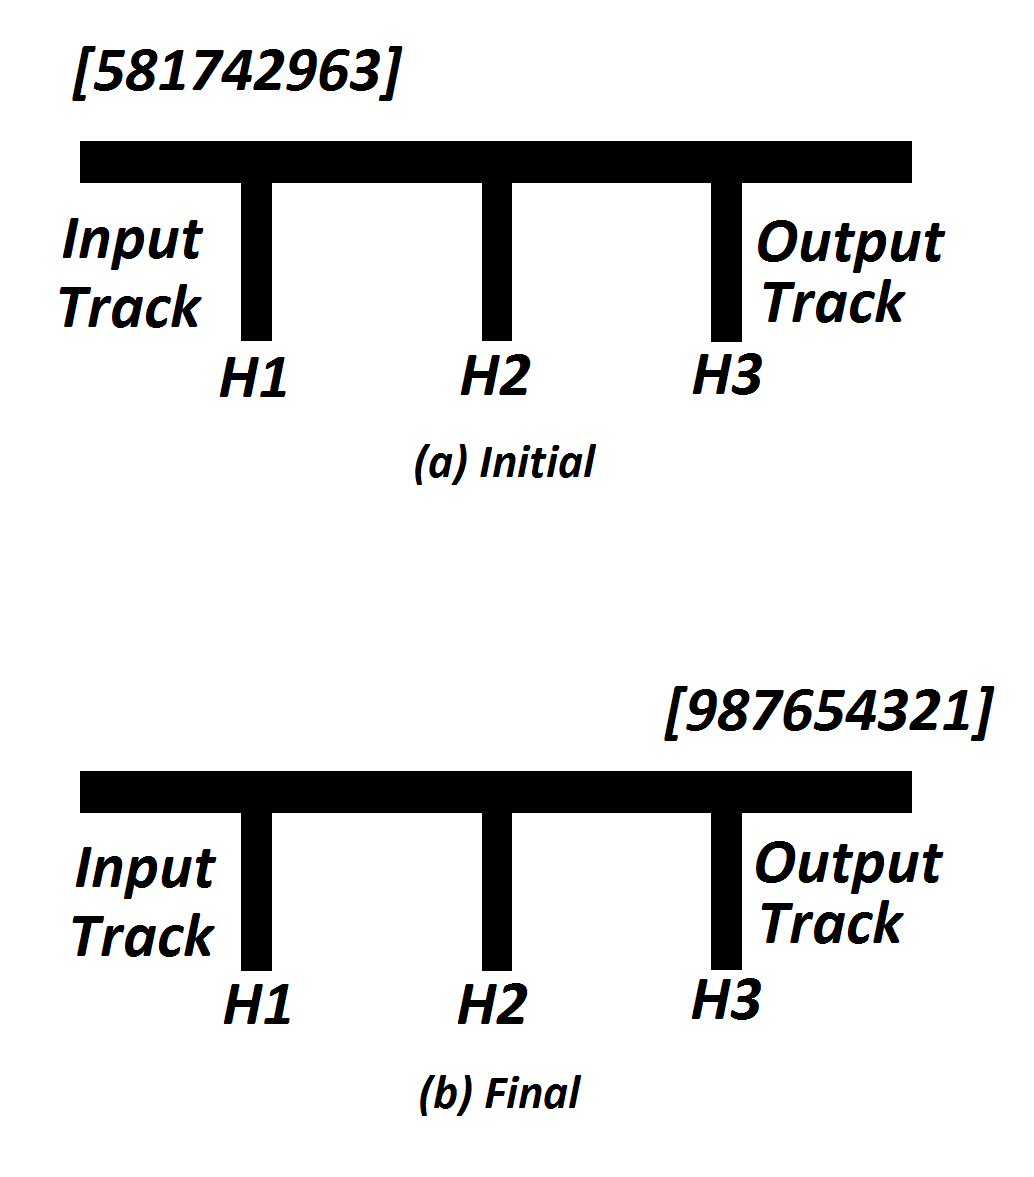
\includegraphics[width=1.0\linewidth,height=6.5in,keepaspectratio]{../images/16.png}
\end{center}
\raggedright{}\myfigurewithcaption{16}{Railroad cars example}
\end{minipage}\vspace{0.75cm}


\begin{myitemize}
\item{} Consider the input arrangement from figure , here we note that the car 3 is at the front, so it can\textquotesingle{}t be output yet, as it to be preceded by cars 1 \& 2. So car 3 is detached \& moved to holding track {\bfseries {\bfseries \itshape H1}} {\itshape } \setmainfont[Path=/usr/share/fonts/truetype/cmu/,UprightFont=cmunrm.ttf,BoldFont=cmunbx.ttf,ItalicFont=cmunti.ttf,BoldItalicFont=cmunbi.ttf]{cmunrm.ttf}\setmonofont[Path=/usr/share/fonts/truetype/cmu/,UprightFont=cmuntt.ttf,BoldFont=cmuntb.ttf,ItalicFont=cmunit.ttf,BoldItalicFont=cmuntx.ttf]{cmunrm.ttf}.
\item{} The next car 6 can\textquotesingle{}t be output \& it is moved to holding track {\bfseries {\bfseries \itshape H2}} {\itshape } \setmainfont[Path=/usr/share/fonts/truetype/cmu/,UprightFont=cmunrm.ttf,BoldFont=cmunbx.ttf,ItalicFont=cmunti.ttf,BoldItalicFont=cmunbi.ttf]{cmunrm.ttf}\setmonofont[Path=/usr/share/fonts/truetype/cmu/,UprightFont=cmuntt.ttf,BoldFont=cmuntb.ttf,ItalicFont=cmunit.ttf,BoldItalicFont=cmuntx.ttf]{cmunrm.ttf}. Because we have to output car 3 before car 6 \& this will not possible if we move car 6 to holding track {\bfseries {\bfseries \itshape H1}} {\itshape } \setmainfont[Path=/usr/share/fonts/truetype/cmu/,UprightFont=cmunrm.ttf,BoldFont=cmunbx.ttf,ItalicFont=cmunti.ttf,BoldItalicFont=cmunbi.ttf]{cmunrm.ttf}\setmonofont[Path=/usr/share/fonts/truetype/cmu/,UprightFont=cmuntt.ttf,BoldFont=cmuntb.ttf,ItalicFont=cmunit.ttf,BoldItalicFont=cmuntx.ttf]{cmunrm.ttf}.
\item{} Now it\textquotesingle{}s obvious that we move car 9 to {\bfseries {\bfseries \itshape H3}} {\itshape } \setmainfont[Path=/usr/share/fonts/truetype/cmu/,UprightFont=cmunrm.ttf,BoldFont=cmunbx.ttf,ItalicFont=cmunti.ttf,BoldItalicFont=cmunbi.ttf]{cmunrm.ttf}\setmonofont[Path=/usr/share/fonts/truetype/cmu/,UprightFont=cmuntt.ttf,BoldFont=cmuntb.ttf,ItalicFont=cmunit.ttf,BoldItalicFont=cmuntx.ttf]{cmunrm.ttf}.
\end{myitemize}

The requirement of rearrangement of cars on any holding track is that the cars should be preferred  to arrange in ascending order from top to bottom. 
\begin{myitemize}
\item{} So car 2 is now moved to holding track H1 so that it satisfies the previous statement. If we move car 2 to H2 or H3, then we\textquotesingle{}ve no place to move cars 4,5,7,8.{\bfseries {\bfseries \itshape The least restrictions on future car placement arise when the new car λ is moved to the holding track that has a car at its top with smallest label Ψ such that λ <{} Ψ. We may call it an assignment rule to decide whether a particular car belongs to a specific holding track.}} {\itshape } \setmainfont[Path=/usr/share/fonts/truetype/cmu/,UprightFont=cmunrm.ttf,BoldFont=cmunbx.ttf,ItalicFont=cmunti.ttf,BoldItalicFont=cmunbi.ttf]{cmunrm.ttf}\setmonofont[Path=/usr/share/fonts/truetype/cmu/,UprightFont=cmuntt.ttf,BoldFont=cmuntb.ttf,ItalicFont=cmunit.ttf,BoldItalicFont=cmuntx.ttf]{cmunrm.ttf} 
\item{} When car 4 is considered, there are three places to move the car H1,H2,H3. The top of these tracks are 2,6,9.So using above mentioned Assignment rule, we move car 4 to H2.
\item{} The car 7 is moved to H3.
\item{} The next car 1 has the least label, so it\textquotesingle{}s moved to output track.
\item{} Now it\textquotesingle{}s time for car 2 \& 3 to output which are from H1(in short all the cars from H1 are appended to car 1 on output track).
\end{myitemize}

The car 4 is moved to output track. No other cars can be moved to output track at this time.
\begin{myitemize}
\item{} The next car 8 is moved to holding track H1.
\item{} Car 5 is output from input track. Car 6 is moved to output track from H2, so is the 7 from H3,8 from H1 \& 9 from H3.
\end{myitemize}


\subsubsection{Quicksort}
\label{56}

Sorting means arranging a group of elements in a particular order. Be it ascending or descending, by cardinality or alphabetical order or variations thereof.  The resulting ordering possibilities will only be limited by the type of the source elements. 

Quicksort is an algorithm of the {\itshape divide and conquer} \setmainfont[Path=/usr/share/fonts/truetype/cmu/,UprightFont=cmunrm.ttf,BoldFont=cmunbx.ttf,ItalicFont=cmunti.ttf,BoldItalicFont=cmunbi.ttf]{cmunrm.ttf}\setmonofont[Path=/usr/share/fonts/truetype/cmu/,UprightFont=cmuntt.ttf,BoldFont=cmuntb.ttf,ItalicFont=cmunit.ttf,BoldItalicFont=cmuntx.ttf]{cmunrm.ttf} type. In this method, to sort a set of numbers, we reduce it to two smaller sets, and then sort these smaller sets.

This can be explained with the help of the following example:

Suppose {\bfseries \setmainfont[Path=/usr/share/fonts/truetype/cmu/,UprightFont=cmunrm.ttf,BoldFont=cmunbx.ttf,ItalicFont=cmunti.ttf,BoldItalicFont=cmunbi.ttf]{cmunbx.ttf}\setmonofont[Path=/usr/share/fonts/truetype/cmu/,UprightFont=cmuntt.ttf,BoldFont=cmuntb.ttf,ItalicFont=cmunit.ttf,BoldItalicFont=cmuntx.ttf]{cmunbx.ttf}\bfseries A} \setmainfont[Path=/usr/share/fonts/truetype/cmu/,UprightFont=cmunrm.ttf,BoldFont=cmunbx.ttf,ItalicFont=cmunti.ttf,BoldItalicFont=cmunbi.ttf]{cmunrm.ttf}\setmonofont[Path=/usr/share/fonts/truetype/cmu/,UprightFont=cmuntt.ttf,BoldFont=cmuntb.ttf,ItalicFont=cmunit.ttf,BoldItalicFont=cmuntx.ttf]{cmunrm.ttf} is a list of the following numbers:



\begin{minipage}{1.0\linewidth}
\begin{center}
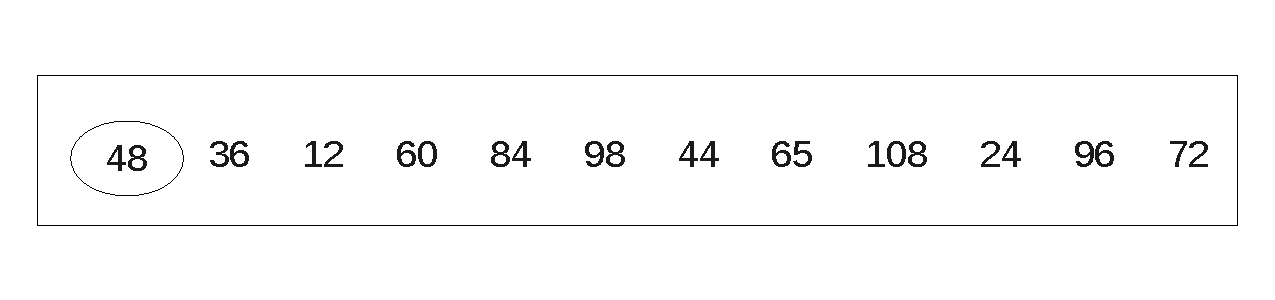
\includegraphics[width=1.0\linewidth,height=6.5in,keepaspectratio]{../images/17.pdf}
\end{center}
\raggedright{}\myfigurewithoutcaption{17}
\end{minipage}\vspace{0.75cm}



In the reduction step, we find the final position of one of the numbers. In this case, let us assume that we have to find the final position of 48, which is the first number in the list.

To accomplish this, we adopt the following method. Begin with the last number, and move from right to left. Compare each number with 48. If the number is smaller than 48, we stop at that number and swap it with 48.


In our case, the number is 24. Hence, we swap 24 and 48.



\begin{minipage}{1.0\linewidth}
\begin{center}
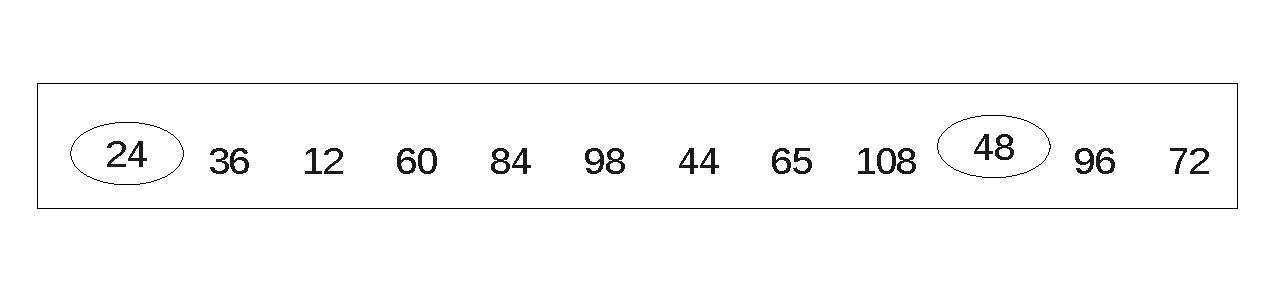
\includegraphics[width=1.0\linewidth,height=6.5in,keepaspectratio]{../images/18.pdf}
\end{center}
\raggedright{}\myfigurewithoutcaption{18}
\end{minipage}\vspace{0.75cm}



The numbers 96 and 72 to the right of 48, are greater than 48.  Now beginning with 24, scan the numbers in the opposite direction, that is from left to right. Compare every number with 48 until you find a number that is greater than 48. 

In this case, it is 60. Therefore we swap 48 and 60.



\begin{minipage}{1.0\linewidth}
\begin{center}
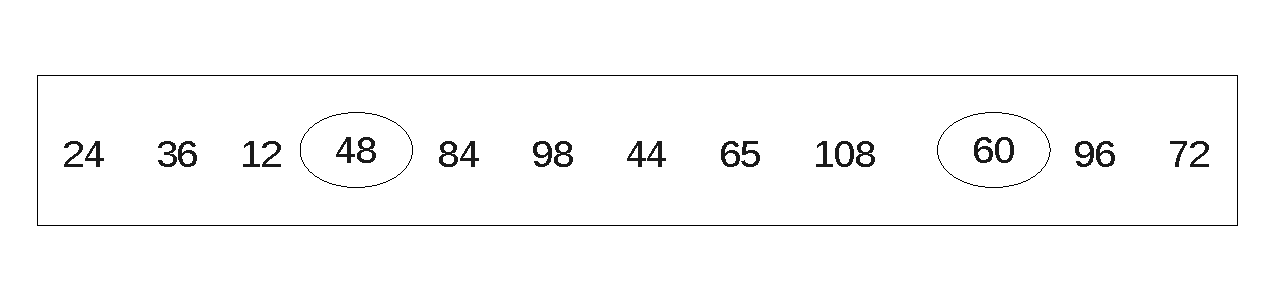
\includegraphics[width=1.0\linewidth,height=6.5in,keepaspectratio]{../images/19.pdf}
\end{center}
\raggedright{}\myfigurewithoutcaption{19}
\end{minipage}\vspace{0.75cm}



Note that the numbers 12, 24 and 36 to the left of 48 are all smaller than 48. Now, start scanning numbers from 60, in the right to left direction. As soon as you find lesser number, swap it with 48.

In this case, it is 44. Swap it with 48. The final result is:



\begin{minipage}{1.0\linewidth}
\begin{center}
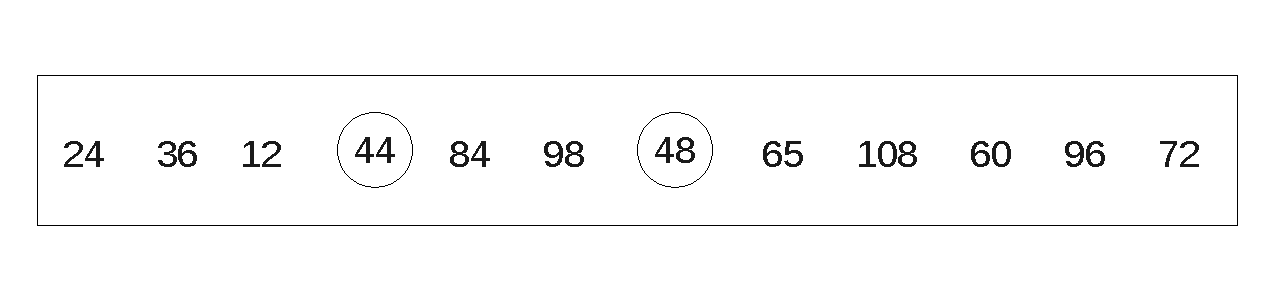
\includegraphics[width=1.0\linewidth,height=6.5in,keepaspectratio]{../images/20.pdf}
\end{center}
\raggedright{}\myfigurewithoutcaption{20}
\end{minipage}\vspace{0.75cm}



Now, beginning with 44, scan the list from left to right, until you find a number greater than 48.

Such a number is 84. Swap it with 48. The final result is:



\begin{minipage}{1.0\linewidth}
\begin{center}
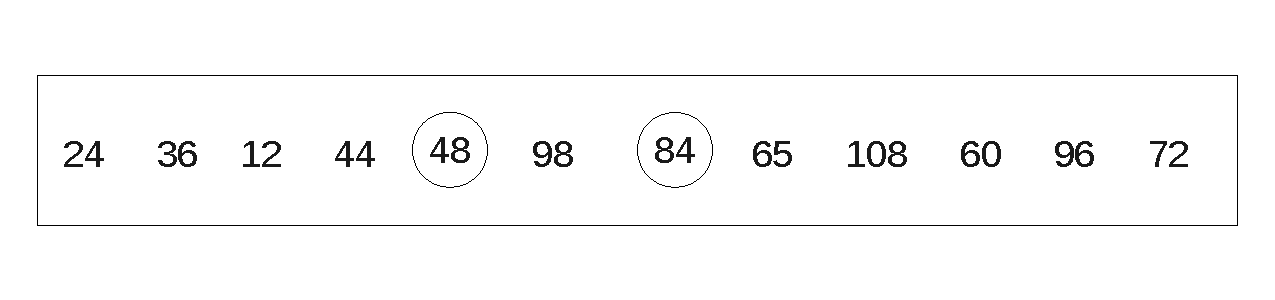
\includegraphics[width=1.0\linewidth,height=6.5in,keepaspectratio]{../images/21.pdf}
\end{center}
\raggedright{}\myfigurewithoutcaption{21}
\end{minipage}\vspace{0.75cm}



Now, beginning with 84, traverse the list from right to left, until you reach a number lesser than 48. We do not find such a number before reaching 48. This means that all the numbers in the list have been scanned and compared with 48. Also, we notice that all numbers less than 48 are to the left of it, and all numbers greater than 48, are to its right.

The final partitions look as follows:



\begin{minipage}{1.0\linewidth}
\begin{center}
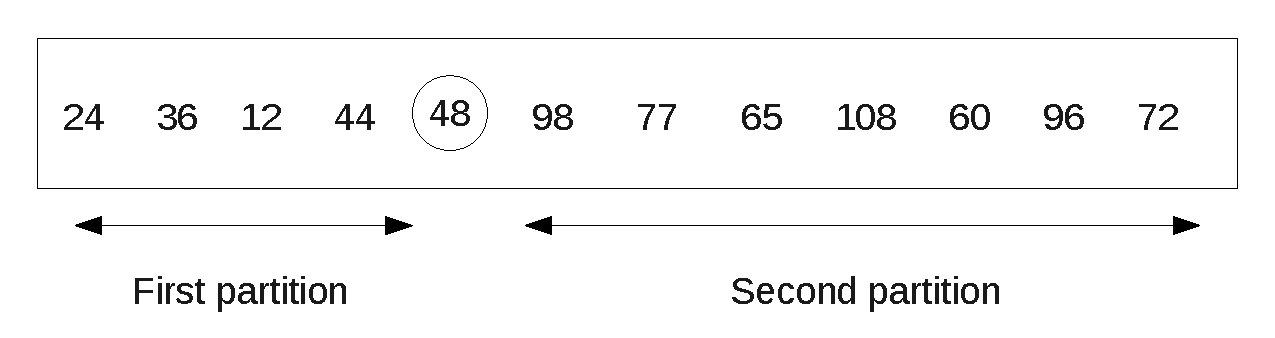
\includegraphics[width=1.0\linewidth,height=6.5in,keepaspectratio]{../images/22.pdf}
\end{center}
\raggedright{}\myfigurewithoutcaption{22}
\end{minipage}\vspace{0.75cm}



Therefore, 48 has been placed in its proper position and now our task is reduced to sorting the two partitions.
This above step of creating partitions can be repeated with every partition containing 2 or more elements. As we can process only a single partition at a time, we should be able to keep track of the other partitions, for future processing.

This is done by using two {\bfseries \setmainfont[Path=/usr/share/fonts/truetype/cmu/,UprightFont=cmunrm.ttf,BoldFont=cmunbx.ttf,ItalicFont=cmunti.ttf,BoldItalicFont=cmunbi.ttf]{cmunbx.ttf}\setmonofont[Path=/usr/share/fonts/truetype/cmu/,UprightFont=cmuntt.ttf,BoldFont=cmuntb.ttf,ItalicFont=cmunit.ttf,BoldItalicFont=cmuntx.ttf]{cmunbx.ttf}\bfseries stacks} \setmainfont[Path=/usr/share/fonts/truetype/cmu/,UprightFont=cmunrm.ttf,BoldFont=cmunbx.ttf,ItalicFont=cmunti.ttf,BoldItalicFont=cmunbi.ttf]{cmunrm.ttf}\setmonofont[Path=/usr/share/fonts/truetype/cmu/,UprightFont=cmuntt.ttf,BoldFont=cmuntb.ttf,ItalicFont=cmunit.ttf,BoldItalicFont=cmuntx.ttf]{cmunrm.ttf} called LOWERBOUND and UPPERBOUND, to temporarily store these partitions. The addresses of the first and last elements of the partitions are pushed into the LOWERBOUND and UPPERBOUND stacks respectively. Now, the above reduction step is applied to the partitions only after its boundary values are {\itshape popped} \setmainfont[Path=/usr/share/fonts/truetype/cmu/,UprightFont=cmunrm.ttf,BoldFont=cmunbx.ttf,ItalicFont=cmunti.ttf,BoldItalicFont=cmunbi.ttf]{cmunrm.ttf}\setmonofont[Path=/usr/share/fonts/truetype/cmu/,UprightFont=cmuntt.ttf,BoldFont=cmuntb.ttf,ItalicFont=cmunit.ttf,BoldItalicFont=cmuntx.ttf]{cmunrm.ttf} from the stack.

We can understand this from the following example:

Take the above list A with 12 elements. The algorithm starts by pushing the boundary values of A, that is 1 and 12 into the LOWERBOUND and UPPERBOUND stacks respectively.  Therefore the stacks look as follows:
\\

\TemplateSpaceIndent{$\text{ }${}$\text{ }${}$\text{ }${}$\text{ }${}$\text{ }${}LOWERBOUND:$\text{ }${}$\text{ }${}1$\text{ }${}$\text{ }${}$\text{ }${}$\text{ }${}$\text{ }${}$\text{ }${}$\text{ }${}$\text{ }${}$\text{ }${}$\text{ }${}$\text{ }${}$\text{ }${}$\text{ }${}$\text{ }${}$\text{ }${}$\text{ }${}$\text{ }${}$\text{ }${}$\text{ }${}UPPERBOUND:$\text{ }${}$\text{ }${}12}


To perform the reduction step, the values of the stack top are popped from the stack. Therefore, both the stacks become empty.
\\

\TemplateSpaceIndent{$\text{ }${}$\text{ }${}$\text{ }${}$\text{ }${}$\text{ }${}LOWERBOUND:$\text{ }${}$\text{ }${}\{empty\}$\text{ }${}$\text{ }${}$\text{ }${}$\text{ }${}$\text{ }${}$\text{ }${}$\text{ }${}$\text{ }${}$\text{ }${}$\text{ }${}$\text{ }${}$\text{ }${}$\text{ }${}$\text{ }${}$\text{ }${}$\text{ }${}UPPERBOUND:$\text{ }${}\{empty\}}


Now, the reduction step causes 48 to be fixed to the 5th position and creates two partitions, one from position 1 to 4 and the other from position 6 to 12. Hence, the values 1 and 6 are pushed into the LOWERBOUND stack and 4 and 12 are pushed into the UPPERBOUND stack.
\\

\TemplateSpaceIndent{$\text{ }${}$\text{ }${}$\text{ }${}$\text{ }${}$\text{ }${}LOWERBOUND:$\text{ }${}$\text{ }${}1,$\text{ }${}6$\text{ }${}$\text{ }${}$\text{ }${}$\text{ }${}$\text{ }${}$\text{ }${}$\text{ }${}$\text{ }${}$\text{ }${}$\text{ }${}$\text{ }${}$\text{ }${}$\text{ }${}$\text{ }${}$\text{ }${}$\text{ }${}$\text{ }${}$\text{ }${}$\text{ }${}UPPERBOUND:$\text{ }${}4,$\text{ }${}12}


For applying the reduction step again, the values at the stack top are popped. Therefore, the values 6 and 12 are popped. Therefore the stacks look like:
\\

\TemplateSpaceIndent{$\text{ }${}$\text{ }${}$\text{ }${}$\text{ }${}$\text{ }${}LOWERBOUND:$\text{ }${}$\text{ }${}1$\text{ }${}$\text{ }${}$\text{ }${}$\text{ }${}$\text{ }${}$\text{ }${}$\text{ }${}$\text{ }${}$\text{ }${}$\text{ }${}$\text{ }${}$\text{ }${}$\text{ }${}$\text{ }${}$\text{ }${}$\text{ }${}$\text{ }${}$\text{ }${}$\text{ }${}$\text{ }${}$\text{ }${}$\text{ }${}UPPERBOUND:$\text{ }${}4}


The reduction step is now applied to the second partition, that is from the 6th to 12th element.



\begin{minipage}{1.0\linewidth}
\begin{center}
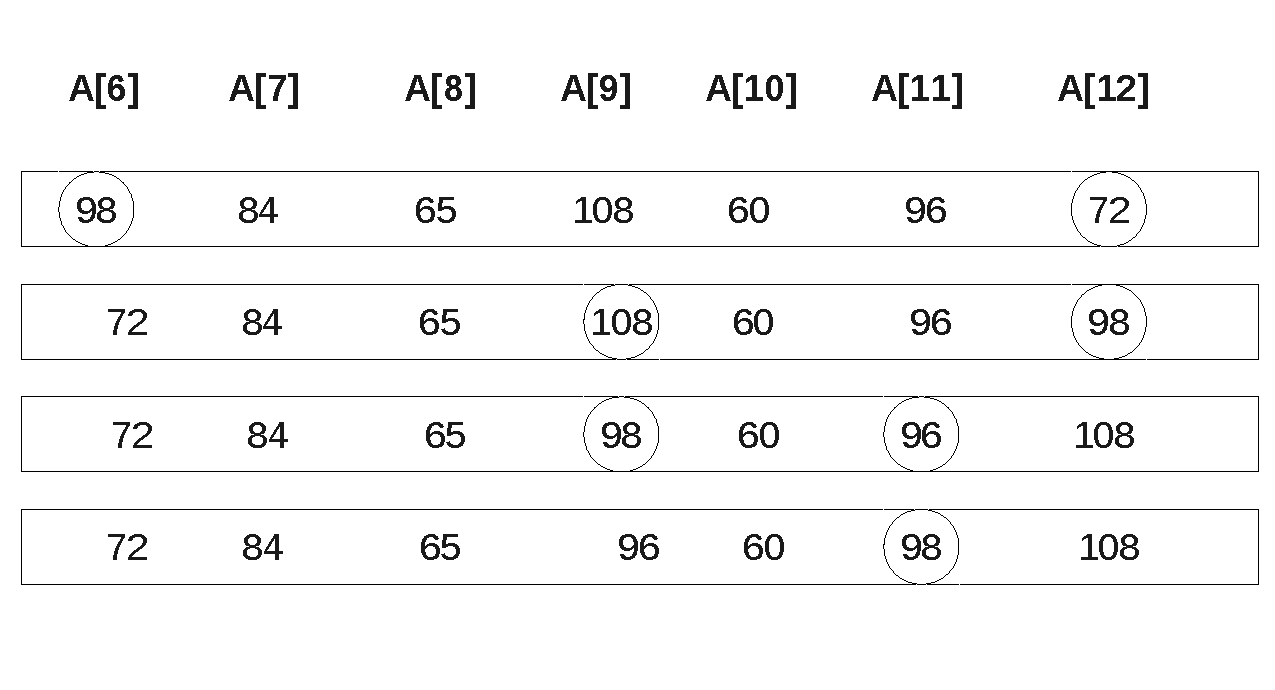
\includegraphics[width=1.0\linewidth,height=6.5in,keepaspectratio]{../images/23.pdf}
\end{center}
\raggedright{}\myfigurewithoutcaption{23}
\end{minipage}\vspace{0.75cm}



After the reduction step, 98 is fixed in the 11th position. So, the second partition has only one element. Therefore, we push the upper and lower boundary values of the first partition onto the stack. So, the stacks are as follows:
\\

\TemplateSpaceIndent{$\text{ }${}$\text{ }${}$\text{ }${}$\text{ }${}$\text{ }${}LOWERBOUND:$\text{ }${}$\text{ }${}1,$\text{ }${}6$\text{ }${}$\text{ }${}$\text{ }${}$\text{ }${}$\text{ }${}$\text{ }${}$\text{ }${}$\text{ }${}$\text{ }${}$\text{ }${}$\text{ }${}$\text{ }${}$\text{ }${}$\text{ }${}$\text{ }${}$\text{ }${}$\text{ }${}$\text{ }${}$\text{ }${}UPPERBOUND:$\text{ }${}$\text{ }${}4,$\text{ }${}10}


The processing proceeds in the following way and ends when the stacks do not contain any upper and lower bounds of the partition to be processed, and the list gets sorted.
\subsubsection{The Stock Span Problem}
\label{57}


\begin{minipage}{0.81250\textwidth}
\begin{center}
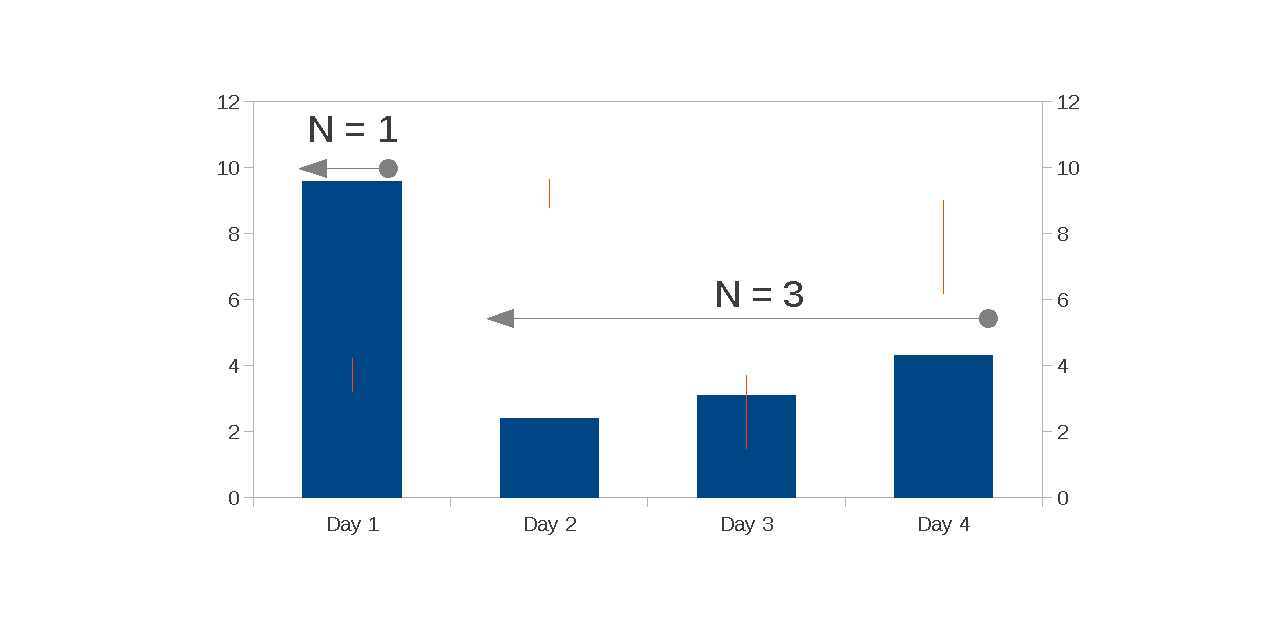
\includegraphics[width=1.0\textwidth,height=6.5in,keepaspectratio]{../images/24.pdf}
\end{center}
\raggedright{}\myfigurewithcaption{24}{The Stockspan Problem}
\end{minipage}\vspace{0.75cm}


In the stock span problem, we will solve a financial problem with the help of stacks.

Suppose, for a stock, we have a series of {\itshape n} \setmainfont[Path=/usr/share/fonts/truetype/cmu/,UprightFont=cmunrm.ttf,BoldFont=cmunbx.ttf,ItalicFont=cmunti.ttf,BoldItalicFont=cmunbi.ttf]{cmunrm.ttf}\setmonofont[Path=/usr/share/fonts/truetype/cmu/,UprightFont=cmuntt.ttf,BoldFont=cmuntb.ttf,ItalicFont=cmunit.ttf,BoldItalicFont=cmuntx.ttf]{cmunrm.ttf} daily price quotes, the {\itshape span} \setmainfont[Path=/usr/share/fonts/truetype/cmu/,UprightFont=cmunrm.ttf,BoldFont=cmunbx.ttf,ItalicFont=cmunti.ttf,BoldItalicFont=cmunbi.ttf]{cmunrm.ttf}\setmonofont[Path=/usr/share/fonts/truetype/cmu/,UprightFont=cmuntt.ttf,BoldFont=cmuntb.ttf,ItalicFont=cmunit.ttf,BoldItalicFont=cmuntx.ttf]{cmunrm.ttf} of the stock\textquotesingle{}s price on a particular day is defined as the maximum number of consecutive days for which the price of the stock on the current day is less than or equal to its price on that day.
\paragraph{An algorithm which has Quadratic Time Complexity}
{$\text{ }$}\newline\label{58}

{\bfseries \setmainfont[Path=/usr/share/fonts/truetype/cmu/,UprightFont=cmunrm.ttf,BoldFont=cmunbx.ttf,ItalicFont=cmunti.ttf,BoldItalicFont=cmunbi.ttf]{cmunbx.ttf}\setmonofont[Path=/usr/share/fonts/truetype/cmu/,UprightFont=cmuntt.ttf,BoldFont=cmuntb.ttf,ItalicFont=cmunit.ttf,BoldItalicFont=cmuntx.ttf]{cmunbx.ttf}\bfseries Input:} \setmainfont[Path=/usr/share/fonts/truetype/cmu/,UprightFont=cmunrm.ttf,BoldFont=cmunbx.ttf,ItalicFont=cmunti.ttf,BoldItalicFont=cmunbi.ttf]{cmunrm.ttf}\setmonofont[Path=/usr/share/fonts/truetype/cmu/,UprightFont=cmuntt.ttf,BoldFont=cmuntb.ttf,ItalicFont=cmunit.ttf,BoldItalicFont=cmuntx.ttf]{cmunrm.ttf} An array {\itshape P} \setmainfont[Path=/usr/share/fonts/truetype/cmu/,UprightFont=cmunrm.ttf,BoldFont=cmunbx.ttf,ItalicFont=cmunti.ttf,BoldItalicFont=cmunbi.ttf]{cmunrm.ttf}\setmonofont[Path=/usr/share/fonts/truetype/cmu/,UprightFont=cmuntt.ttf,BoldFont=cmuntb.ttf,ItalicFont=cmunit.ttf,BoldItalicFont=cmuntx.ttf]{cmunrm.ttf} with {\itshape n} \setmainfont[Path=/usr/share/fonts/truetype/cmu/,UprightFont=cmunrm.ttf,BoldFont=cmunbx.ttf,ItalicFont=cmunti.ttf,BoldItalicFont=cmunbi.ttf]{cmunrm.ttf}\setmonofont[Path=/usr/share/fonts/truetype/cmu/,UprightFont=cmuntt.ttf,BoldFont=cmuntb.ttf,ItalicFont=cmunit.ttf,BoldItalicFont=cmuntx.ttf]{cmunrm.ttf} elements

{\bfseries \setmainfont[Path=/usr/share/fonts/truetype/cmu/,UprightFont=cmunrm.ttf,BoldFont=cmunbx.ttf,ItalicFont=cmunti.ttf,BoldItalicFont=cmunbi.ttf]{cmunbx.ttf}\setmonofont[Path=/usr/share/fonts/truetype/cmu/,UprightFont=cmuntt.ttf,BoldFont=cmuntb.ttf,ItalicFont=cmunit.ttf,BoldItalicFont=cmuntx.ttf]{cmunbx.ttf}\bfseries Output:} \setmainfont[Path=/usr/share/fonts/truetype/cmu/,UprightFont=cmunrm.ttf,BoldFont=cmunbx.ttf,ItalicFont=cmunti.ttf,BoldItalicFont=cmunbi.ttf]{cmunrm.ttf}\setmonofont[Path=/usr/share/fonts/truetype/cmu/,UprightFont=cmuntt.ttf,BoldFont=cmuntb.ttf,ItalicFont=cmunit.ttf,BoldItalicFont=cmuntx.ttf]{cmunrm.ttf} An array {\itshape S} \setmainfont[Path=/usr/share/fonts/truetype/cmu/,UprightFont=cmunrm.ttf,BoldFont=cmunbx.ttf,ItalicFont=cmunti.ttf,BoldItalicFont=cmunbi.ttf]{cmunrm.ttf}\setmonofont[Path=/usr/share/fonts/truetype/cmu/,UprightFont=cmuntt.ttf,BoldFont=cmuntb.ttf,ItalicFont=cmunit.ttf,BoldItalicFont=cmuntx.ttf]{cmunrm.ttf}  of {\itshape n} \setmainfont[Path=/usr/share/fonts/truetype/cmu/,UprightFont=cmunrm.ttf,BoldFont=cmunbx.ttf,ItalicFont=cmunti.ttf,BoldItalicFont=cmunbi.ttf]{cmunrm.ttf}\setmonofont[Path=/usr/share/fonts/truetype/cmu/,UprightFont=cmuntt.ttf,BoldFont=cmuntb.ttf,ItalicFont=cmunit.ttf,BoldItalicFont=cmuntx.ttf]{cmunrm.ttf} elements such that P{$\text{[}$}i{$\text{]}$} is the largest integer k such that k <{}= i + 1 and P{$\text{[}$}y{$\text{]}$} <{}= P{$\text{[}$}i{$\text{]}$} for j = i -{} k + 1,.....,i

{\bfseries \setmainfont[Path=/usr/share/fonts/truetype/cmu/,UprightFont=cmunrm.ttf,BoldFont=cmunbx.ttf,ItalicFont=cmunti.ttf,BoldItalicFont=cmunbi.ttf]{cmunbx.ttf}\setmonofont[Path=/usr/share/fonts/truetype/cmu/,UprightFont=cmuntt.ttf,BoldFont=cmuntb.ttf,ItalicFont=cmunit.ttf,BoldItalicFont=cmuntx.ttf]{cmunbx.ttf}\bfseries Algorithm:} \setmainfont[Path=/usr/share/fonts/truetype/cmu/,UprightFont=cmunrm.ttf,BoldFont=cmunbx.ttf,ItalicFont=cmunti.ttf,BoldItalicFont=cmunbi.ttf]{cmunrm.ttf}\setmonofont[Path=/usr/share/fonts/truetype/cmu/,UprightFont=cmuntt.ttf,BoldFont=cmuntb.ttf,ItalicFont=cmunit.ttf,BoldItalicFont=cmuntx.ttf]{cmunrm.ttf}
\\

\TemplateSpaceIndent{$\text{ }${}$\text{ }${}$\text{ }${}$\text{ }${}$\text{ }${}$\text{ }${}$\text{ }${}$\text{ }${}1.$\text{ }${}Initialize$\text{ }${}an$\text{ }${}array$\text{ }${}P$\text{ }${}which$\text{ }${}contains$\text{ }${}the$\text{ }${}daily$\text{ }${}prices$\text{ }${}of$\text{ }${}the$\text{ }${}stocks$\text{ }$\newline{}
$\text{ }${}$\text{ }${}$\text{ }${}$\text{ }${}$\text{ }${}$\text{ }${}$\text{ }${}$\text{ }${}2.$\text{ }${}Initialize$\text{ }${}an$\text{ }${}array$\text{ }${}S$\text{ }${}which$\text{ }${}will$\text{ }${}store$\text{ }${}the$\text{ }${}span$\text{ }${}of$\text{ }${}the$\text{ }${}stock$\text{ }$\newline{}
$\text{ }${}$\text{ }${}$\text{ }${}$\text{ }${}$\text{ }${}$\text{ }${}$\text{ }${}$\text{ }${}3.$\text{ }${}{\bfseries \setmainfont[Path=/usr/share/fonts/truetype/cmu/,UprightFont=cmunrm.ttf,BoldFont=cmunbx.ttf,ItalicFont=cmunti.ttf,BoldItalicFont=cmunbi.ttf]{cmunbx.ttf}\setmonofont[Path=/usr/share/fonts/truetype/cmu/,UprightFont=cmuntt.ttf,BoldFont=cmuntb.ttf,ItalicFont=cmunit.ttf,BoldItalicFont=cmuntx.ttf]{cmunbx.ttf}\bfseries for} $\text{ }${}\setmainfont[Path=/usr/share/fonts/truetype/cmu/,UprightFont=cmunrm.ttf,BoldFont=cmunbx.ttf,ItalicFont=cmunti.ttf,BoldItalicFont=cmunbi.ttf]{cmunrm.ttf}\setmonofont[Path=/usr/share/fonts/truetype/cmu/,UprightFont=cmuntt.ttf,BoldFont=cmuntb.ttf,ItalicFont=cmunit.ttf,BoldItalicFont=cmuntx.ttf]{cmunrm.ttf}i$\text{ }${}=$\text{ }${}0$\text{ }${}to$\text{ }${}i$\text{ }${}=$\text{ }${}n$\text{ }${}-{}$\text{ }${}1$\text{ }$\newline{}
$\text{ }${}$\text{ }${}$\text{ }${}$\text{ }${}$\text{ }${}$\text{ }${}$\text{ }${}$\text{ }${}$\text{ }${}$\text{ }${}$\text{ }${}$\text{ }${}$\text{ }${}$\text{ }${}$\text{ }${}$\text{ }${}3.1$\text{ }${}Initialize$\text{ }${}k$\text{ }${}to$\text{ }${}zero$\text{ }$\newline{}
$\text{ }${}$\text{ }${}$\text{ }${}$\text{ }${}$\text{ }${}$\text{ }${}$\text{ }${}$\text{ }${}$\text{ }${}$\text{ }${}$\text{ }${}$\text{ }${}$\text{ }${}$\text{ }${}$\text{ }${}$\text{ }${}3.2$\text{ }${}Done$\text{ }${}with$\text{ }${}a$\text{ }${}{\itshape false} $\text{ }${}\setmainfont[Path=/usr/share/fonts/truetype/cmu/,UprightFont=cmunrm.ttf,BoldFont=cmunbx.ttf,ItalicFont=cmunti.ttf,BoldItalicFont=cmunbi.ttf]{cmunrm.ttf}\setmonofont[Path=/usr/share/fonts/truetype/cmu/,UprightFont=cmuntt.ttf,BoldFont=cmuntb.ttf,ItalicFont=cmunit.ttf,BoldItalicFont=cmuntx.ttf]{cmunrm.ttf}condition$\text{ }$\newline{}
$\text{ }${}$\text{ }${}$\text{ }${}$\text{ }${}$\text{ }${}$\text{ }${}$\text{ }${}$\text{ }${}$\text{ }${}$\text{ }${}$\text{ }${}$\text{ }${}$\text{ }${}$\text{ }${}$\text{ }${}$\text{ }${}3.3$\text{ }${}{\bfseries \setmainfont[Path=/usr/share/fonts/truetype/cmu/,UprightFont=cmunrm.ttf,BoldFont=cmunbx.ttf,ItalicFont=cmunti.ttf,BoldItalicFont=cmunbi.ttf]{cmunbx.ttf}\setmonofont[Path=/usr/share/fonts/truetype/cmu/,UprightFont=cmuntt.ttf,BoldFont=cmuntb.ttf,ItalicFont=cmunit.ttf,BoldItalicFont=cmuntx.ttf]{cmunbx.ttf}\bfseries repeat} $\text{ }$\newline{}
$\text{ }${}$\text{ }${}$\text{ }${}$\text{ }${}$\text{ }${}$\text{ }${}$\text{ }${}$\text{ }${}$\text{ }${}$\text{ }${}$\text{ }${}$\text{ }${}$\text{ }${}$\text{ }${}$\text{ }${}$\text{ }${}$\text{ }${}$\text{ }${}$\text{ }${}$\text{ }${}$\text{ }${}$\text{ }${}\setmainfont[Path=/usr/share/fonts/truetype/cmu/,UprightFont=cmunrm.ttf,BoldFont=cmunbx.ttf,ItalicFont=cmunti.ttf,BoldItalicFont=cmunbi.ttf]{cmunrm.ttf}\setmonofont[Path=/usr/share/fonts/truetype/cmu/,UprightFont=cmuntt.ttf,BoldFont=cmuntb.ttf,ItalicFont=cmunit.ttf,BoldItalicFont=cmuntx.ttf]{cmunrm.ttf}3.3.1$\text{ }${}if$\text{ }${}($\text{ }${}P{$\text{[}$}i$\text{ }${}-{}$\text{ }${}k{$\text{]}$}$\text{ }${}<{}=$\text{ }${}P{$\text{[}$}i){$\text{]}$}$\text{ }${}then$\text{ }$\newline{}
$\text{ }${}$\text{ }${}$\text{ }${}$\text{ }${}$\text{ }${}$\text{ }${}$\text{ }${}$\text{ }${}$\text{ }${}$\text{ }${}$\text{ }${}$\text{ }${}$\text{ }${}$\text{ }${}$\text{ }${}$\text{ }${}$\text{ }${}$\text{ }${}$\text{ }${}$\text{ }${}$\text{ }${}$\text{ }${}$\text{ }${}$\text{ }${}$\text{ }${}$\text{ }${}$\text{ }${}$\text{ }${}$\text{ }${}$\text{ }${}$\text{ }${}$\text{ }${}Increment$\text{ }${}k$\text{ }${}by$\text{ }${}1$\text{ }$\newline{}
$\text{ }${}$\text{ }${}$\text{ }${}$\text{ }${}$\text{ }${}$\text{ }${}$\text{ }${}$\text{ }${}$\text{ }${}$\text{ }${}$\text{ }${}$\text{ }${}$\text{ }${}$\text{ }${}$\text{ }${}$\text{ }${}$\text{ }${}$\text{ }${}$\text{ }${}$\text{ }${}$\text{ }${}$\text{ }${}3.3.2$\text{ }${}else$\text{ }$\newline{}
$\text{ }${}$\text{ }${}$\text{ }${}$\text{ }${}$\text{ }${}$\text{ }${}$\text{ }${}$\text{ }${}$\text{ }${}$\text{ }${}$\text{ }${}$\text{ }${}$\text{ }${}$\text{ }${}$\text{ }${}$\text{ }${}$\text{ }${}$\text{ }${}$\text{ }${}$\text{ }${}$\text{ }${}$\text{ }${}$\text{ }${}$\text{ }${}$\text{ }${}$\text{ }${}$\text{ }${}$\text{ }${}$\text{ }${}$\text{ }${}$\text{ }${}$\text{ }${}Done$\text{ }${}with$\text{ }${}{\itshape true} $\text{ }${}\setmainfont[Path=/usr/share/fonts/truetype/cmu/,UprightFont=cmunrm.ttf,BoldFont=cmunbx.ttf,ItalicFont=cmunti.ttf,BoldItalicFont=cmunbi.ttf]{cmunrm.ttf}\setmonofont[Path=/usr/share/fonts/truetype/cmu/,UprightFont=cmuntt.ttf,BoldFont=cmuntb.ttf,ItalicFont=cmunit.ttf,BoldItalicFont=cmuntx.ttf]{cmunrm.ttf}condition$\text{ }$\newline{}
$\text{ }${}$\text{ }${}$\text{ }${}$\text{ }${}$\text{ }${}$\text{ }${}$\text{ }${}$\text{ }${}$\text{ }${}$\text{ }${}$\text{ }${}$\text{ }${}$\text{ }${}$\text{ }${}$\text{ }${}$\text{ }${}3.4$\text{ }${}Till$\text{ }${}(k$\text{ }${}>{}$\text{ }${}i)$\text{ }${}or$\text{ }${}done$\text{ }${}with$\text{ }${}processing$\text{ }$\newline{}
$\text{ }${}$\text{ }${}$\text{ }${}$\text{ }${}$\text{ }${}$\text{ }${}$\text{ }${}$\text{ }${}$\text{ }${}$\text{ }${}$\text{ }${}$\text{ }${}$\text{ }${}$\text{ }${}$\text{ }${}$\text{ }${}$\text{ }${}$\text{ }${}$\text{ }${}$\text{ }${}$\text{ }${}$\text{ }${}Assign$\text{ }${}value$\text{ }${}of$\text{ }${}k$\text{ }${}to$\text{ }${}S{$\text{[}$}i{$\text{]}$}$\text{ }${}to$\text{ }${}get$\text{ }${}the$\text{ }${}span$\text{ }${}of$\text{ }${}the$\text{ }${}stock$\text{ }$\newline{}
$\text{ }${}$\text{ }${}$\text{ }${}$\text{ }${}$\text{ }${}$\text{ }${}$\text{ }${}$\text{ }${}4.$\text{ }${}Return$\text{ }${}array$\text{ }${}S}


Now, analyzing this algorithm for running time, we observe:

\begin{myitemize}
\item{} We have initialized the array S at the beginning and returned it at the end. This is a constant time operation, hence takes {\itshape O} \setmainfont[Path=/usr/share/fonts/truetype/cmu/,UprightFont=cmunrm.ttf,BoldFont=cmunbx.ttf,ItalicFont=cmunti.ttf,BoldItalicFont=cmunbi.ttf]{cmunrm.ttf}\setmonofont[Path=/usr/share/fonts/truetype/cmu/,UprightFont=cmuntt.ttf,BoldFont=cmuntb.ttf,ItalicFont=cmunit.ttf,BoldItalicFont=cmuntx.ttf]{cmunrm.ttf}(n) time
\end{myitemize}


\begin{myitemize}
\item{} The {\itshape repeat} \setmainfont[Path=/usr/share/fonts/truetype/cmu/,UprightFont=cmunrm.ttf,BoldFont=cmunbx.ttf,ItalicFont=cmunti.ttf,BoldItalicFont=cmunbi.ttf]{cmunrm.ttf}\setmonofont[Path=/usr/share/fonts/truetype/cmu/,UprightFont=cmuntt.ttf,BoldFont=cmuntb.ttf,ItalicFont=cmunit.ttf,BoldItalicFont=cmuntx.ttf]{cmunrm.ttf} loop is nested within the {\itshape for} \setmainfont[Path=/usr/share/fonts/truetype/cmu/,UprightFont=cmunrm.ttf,BoldFont=cmunbx.ttf,ItalicFont=cmunti.ttf,BoldItalicFont=cmunbi.ttf]{cmunrm.ttf}\setmonofont[Path=/usr/share/fonts/truetype/cmu/,UprightFont=cmuntt.ttf,BoldFont=cmuntb.ttf,ItalicFont=cmunit.ttf,BoldItalicFont=cmuntx.ttf]{cmunrm.ttf} loop. The {\itshape for} \setmainfont[Path=/usr/share/fonts/truetype/cmu/,UprightFont=cmunrm.ttf,BoldFont=cmunbx.ttf,ItalicFont=cmunti.ttf,BoldItalicFont=cmunbi.ttf]{cmunrm.ttf}\setmonofont[Path=/usr/share/fonts/truetype/cmu/,UprightFont=cmuntt.ttf,BoldFont=cmuntb.ttf,ItalicFont=cmunit.ttf,BoldItalicFont=cmuntx.ttf]{cmunrm.ttf} loop, whose counter is {\itshape i} \setmainfont[Path=/usr/share/fonts/truetype/cmu/,UprightFont=cmunrm.ttf,BoldFont=cmunbx.ttf,ItalicFont=cmunti.ttf,BoldItalicFont=cmunbi.ttf]{cmunrm.ttf}\setmonofont[Path=/usr/share/fonts/truetype/cmu/,UprightFont=cmuntt.ttf,BoldFont=cmuntb.ttf,ItalicFont=cmunit.ttf,BoldItalicFont=cmuntx.ttf]{cmunrm.ttf} is executed n times. The statements which are not in the repeat loop, but in the for loop are executed {\itshape n} \setmainfont[Path=/usr/share/fonts/truetype/cmu/,UprightFont=cmunrm.ttf,BoldFont=cmunbx.ttf,ItalicFont=cmunti.ttf,BoldItalicFont=cmunbi.ttf]{cmunrm.ttf}\setmonofont[Path=/usr/share/fonts/truetype/cmu/,UprightFont=cmuntt.ttf,BoldFont=cmuntb.ttf,ItalicFont=cmunit.ttf,BoldItalicFont=cmuntx.ttf]{cmunrm.ttf} times. Therefore these statements and the incrementing and condition testing of i take {\itshape O} \setmainfont[Path=/usr/share/fonts/truetype/cmu/,UprightFont=cmunrm.ttf,BoldFont=cmunbx.ttf,ItalicFont=cmunti.ttf,BoldItalicFont=cmunbi.ttf]{cmunrm.ttf}\setmonofont[Path=/usr/share/fonts/truetype/cmu/,UprightFont=cmuntt.ttf,BoldFont=cmuntb.ttf,ItalicFont=cmunit.ttf,BoldItalicFont=cmuntx.ttf]{cmunrm.ttf}(n) time.
\end{myitemize}


\begin{myitemize}
\item{} In repetition of i for the outer for loop, the body of the inner {\itshape repeat} \setmainfont[Path=/usr/share/fonts/truetype/cmu/,UprightFont=cmunrm.ttf,BoldFont=cmunbx.ttf,ItalicFont=cmunti.ttf,BoldItalicFont=cmunbi.ttf]{cmunrm.ttf}\setmonofont[Path=/usr/share/fonts/truetype/cmu/,UprightFont=cmuntt.ttf,BoldFont=cmuntb.ttf,ItalicFont=cmunit.ttf,BoldItalicFont=cmuntx.ttf]{cmunrm.ttf} loop is executed maximum i + 1 times. In the worst case, element S{$\text{[}$}i{$\text{]}$} is greater than all the previous elements. So, testing for the if condition, the statement after that, as well as testing the until condition, will be performed i + 1 times during iteration i for the outer for loop. Hence, the total time taken by the inner loop is {\itshape O} \setmainfont[Path=/usr/share/fonts/truetype/cmu/,UprightFont=cmunrm.ttf,BoldFont=cmunbx.ttf,ItalicFont=cmunti.ttf,BoldItalicFont=cmunbi.ttf]{cmunrm.ttf}\setmonofont[Path=/usr/share/fonts/truetype/cmu/,UprightFont=cmuntt.ttf,BoldFont=cmuntb.ttf,ItalicFont=cmunit.ttf,BoldItalicFont=cmuntx.ttf]{cmunrm.ttf}(n(n + 1)/2), which is {\itshape O} \setmainfont[Path=/usr/share/fonts/truetype/cmu/,UprightFont=cmunrm.ttf,BoldFont=cmunbx.ttf,ItalicFont=cmunti.ttf,BoldItalicFont=cmunbi.ttf]{cmunrm.ttf}\setmonofont[Path=/usr/share/fonts/truetype/cmu/,UprightFont=cmuntt.ttf,BoldFont=cmuntb.ttf,ItalicFont=cmunit.ttf,BoldItalicFont=cmuntx.ttf]{cmunrm.ttf}({$n^2 $})
\end{myitemize}


The running time of all these steps is calculated by adding the time taken by all these three steps. The first two terms are {\itshape O} \setmainfont[Path=/usr/share/fonts/truetype/cmu/,UprightFont=cmunrm.ttf,BoldFont=cmunbx.ttf,ItalicFont=cmunti.ttf,BoldItalicFont=cmunbi.ttf]{cmunrm.ttf}\setmonofont[Path=/usr/share/fonts/truetype/cmu/,UprightFont=cmuntt.ttf,BoldFont=cmuntb.ttf,ItalicFont=cmunit.ttf,BoldItalicFont=cmuntx.ttf]{cmunrm.ttf}({$ n $}) while the last term is {\itshape O} \setmainfont[Path=/usr/share/fonts/truetype/cmu/,UprightFont=cmunrm.ttf,BoldFont=cmunbx.ttf,ItalicFont=cmunti.ttf,BoldItalicFont=cmunbi.ttf]{cmunrm.ttf}\setmonofont[Path=/usr/share/fonts/truetype/cmu/,UprightFont=cmuntt.ttf,BoldFont=cmuntb.ttf,ItalicFont=cmunit.ttf,BoldItalicFont=cmuntx.ttf]{cmunrm.ttf}({$n^2 $}). Therefore the total running time of the algorithm is {\itshape O} \setmainfont[Path=/usr/share/fonts/truetype/cmu/,UprightFont=cmunrm.ttf,BoldFont=cmunbx.ttf,ItalicFont=cmunti.ttf,BoldItalicFont=cmunbi.ttf]{cmunrm.ttf}\setmonofont[Path=/usr/share/fonts/truetype/cmu/,UprightFont=cmuntt.ttf,BoldFont=cmuntb.ttf,ItalicFont=cmunit.ttf,BoldItalicFont=cmuntx.ttf]{cmunrm.ttf}({$n^2 $}).
\paragraph{An algorithm that has Linear Time Complexity}
{$\text{ }$}\newline\label{59}

In order to calculate the span more efficiently, we see that the span on a particular day can be easily calculated if we know the closest day before {\itshape i} \setmainfont[Path=/usr/share/fonts/truetype/cmu/,UprightFont=cmunrm.ttf,BoldFont=cmunbx.ttf,ItalicFont=cmunti.ttf,BoldItalicFont=cmunbi.ttf]{cmunrm.ttf}\setmonofont[Path=/usr/share/fonts/truetype/cmu/,UprightFont=cmuntt.ttf,BoldFont=cmuntb.ttf,ItalicFont=cmunit.ttf,BoldItalicFont=cmuntx.ttf]{cmunrm.ttf} , such that the price of the stocks on that day was higher than the price of the stocks on the present day. If there exists such a day, we can represent it by h(i) and initialize h(i) to be -{}1.

Therefore the span of a particular day is given by the formula,
s = i -{} h(i).

To implement this logic, we use a stack as an abstract data type to store the days i, h(i), h(h(i)) and so on. When we go from day i-{}1 to i, we pop the days when the price of the stock was less than or equal to p(i) and then push the value of day {\itshape i} \setmainfont[Path=/usr/share/fonts/truetype/cmu/,UprightFont=cmunrm.ttf,BoldFont=cmunbx.ttf,ItalicFont=cmunti.ttf,BoldItalicFont=cmunbi.ttf]{cmunrm.ttf}\setmonofont[Path=/usr/share/fonts/truetype/cmu/,UprightFont=cmuntt.ttf,BoldFont=cmuntb.ttf,ItalicFont=cmunit.ttf,BoldItalicFont=cmuntx.ttf]{cmunrm.ttf} back into the stack.

Here, we assume that the stack is implemented by operations that take {\itshape O} \setmainfont[Path=/usr/share/fonts/truetype/cmu/,UprightFont=cmunrm.ttf,BoldFont=cmunbx.ttf,ItalicFont=cmunti.ttf,BoldItalicFont=cmunbi.ttf]{cmunrm.ttf}\setmonofont[Path=/usr/share/fonts/truetype/cmu/,UprightFont=cmuntt.ttf,BoldFont=cmuntb.ttf,ItalicFont=cmunit.ttf,BoldItalicFont=cmuntx.ttf]{cmunrm.ttf}(1) that is constant time. The algorithm is as follows:

{\bfseries \setmainfont[Path=/usr/share/fonts/truetype/cmu/,UprightFont=cmunrm.ttf,BoldFont=cmunbx.ttf,ItalicFont=cmunti.ttf,BoldItalicFont=cmunbi.ttf]{cmunbx.ttf}\setmonofont[Path=/usr/share/fonts/truetype/cmu/,UprightFont=cmuntt.ttf,BoldFont=cmuntb.ttf,ItalicFont=cmunit.ttf,BoldItalicFont=cmuntx.ttf]{cmunbx.ttf}\bfseries Input:} \setmainfont[Path=/usr/share/fonts/truetype/cmu/,UprightFont=cmunrm.ttf,BoldFont=cmunbx.ttf,ItalicFont=cmunti.ttf,BoldItalicFont=cmunbi.ttf]{cmunrm.ttf}\setmonofont[Path=/usr/share/fonts/truetype/cmu/,UprightFont=cmuntt.ttf,BoldFont=cmuntb.ttf,ItalicFont=cmunit.ttf,BoldItalicFont=cmuntx.ttf]{cmunrm.ttf} An array P with {\itshape n} \setmainfont[Path=/usr/share/fonts/truetype/cmu/,UprightFont=cmunrm.ttf,BoldFont=cmunbx.ttf,ItalicFont=cmunti.ttf,BoldItalicFont=cmunbi.ttf]{cmunrm.ttf}\setmonofont[Path=/usr/share/fonts/truetype/cmu/,UprightFont=cmuntt.ttf,BoldFont=cmuntb.ttf,ItalicFont=cmunit.ttf,BoldItalicFont=cmuntx.ttf]{cmunrm.ttf} elements and an empty stack N

{\bfseries \setmainfont[Path=/usr/share/fonts/truetype/cmu/,UprightFont=cmunrm.ttf,BoldFont=cmunbx.ttf,ItalicFont=cmunti.ttf,BoldItalicFont=cmunbi.ttf]{cmunbx.ttf}\setmonofont[Path=/usr/share/fonts/truetype/cmu/,UprightFont=cmuntt.ttf,BoldFont=cmuntb.ttf,ItalicFont=cmunit.ttf,BoldItalicFont=cmuntx.ttf]{cmunbx.ttf}\bfseries Output:} \setmainfont[Path=/usr/share/fonts/truetype/cmu/,UprightFont=cmunrm.ttf,BoldFont=cmunbx.ttf,ItalicFont=cmunti.ttf,BoldItalicFont=cmunbi.ttf]{cmunrm.ttf}\setmonofont[Path=/usr/share/fonts/truetype/cmu/,UprightFont=cmuntt.ttf,BoldFont=cmuntb.ttf,ItalicFont=cmunit.ttf,BoldItalicFont=cmuntx.ttf]{cmunrm.ttf} An array {\itshape S} \setmainfont[Path=/usr/share/fonts/truetype/cmu/,UprightFont=cmunrm.ttf,BoldFont=cmunbx.ttf,ItalicFont=cmunti.ttf,BoldItalicFont=cmunbi.ttf]{cmunrm.ttf}\setmonofont[Path=/usr/share/fonts/truetype/cmu/,UprightFont=cmuntt.ttf,BoldFont=cmuntb.ttf,ItalicFont=cmunit.ttf,BoldItalicFont=cmuntx.ttf]{cmunrm.ttf}  of {\itshape n} \setmainfont[Path=/usr/share/fonts/truetype/cmu/,UprightFont=cmunrm.ttf,BoldFont=cmunbx.ttf,ItalicFont=cmunti.ttf,BoldItalicFont=cmunbi.ttf]{cmunrm.ttf}\setmonofont[Path=/usr/share/fonts/truetype/cmu/,UprightFont=cmuntt.ttf,BoldFont=cmuntb.ttf,ItalicFont=cmunit.ttf,BoldItalicFont=cmuntx.ttf]{cmunrm.ttf} elements such that P{$\text{[}$}i{$\text{]}$} is the largest integer k such that k <{}= i + 1 and P{$\text{[}$}y{$\text{]}$} <{}= P{$\text{[}$}i{$\text{]}$} for j = i -{} k + 1,.....,i

{\bfseries \setmainfont[Path=/usr/share/fonts/truetype/cmu/,UprightFont=cmunrm.ttf,BoldFont=cmunbx.ttf,ItalicFont=cmunti.ttf,BoldItalicFont=cmunbi.ttf]{cmunbx.ttf}\setmonofont[Path=/usr/share/fonts/truetype/cmu/,UprightFont=cmuntt.ttf,BoldFont=cmuntb.ttf,ItalicFont=cmunit.ttf,BoldItalicFont=cmuntx.ttf]{cmunbx.ttf}\bfseries Algorithm:} \setmainfont[Path=/usr/share/fonts/truetype/cmu/,UprightFont=cmunrm.ttf,BoldFont=cmunbx.ttf,ItalicFont=cmunti.ttf,BoldItalicFont=cmunbi.ttf]{cmunrm.ttf}\setmonofont[Path=/usr/share/fonts/truetype/cmu/,UprightFont=cmuntt.ttf,BoldFont=cmuntb.ttf,ItalicFont=cmunit.ttf,BoldItalicFont=cmuntx.ttf]{cmunrm.ttf}
\\

\TemplateSpaceIndent{$\text{ }${}$\text{ }${}$\text{ }${}$\text{ }${}$\text{ }${}$\text{ }${}$\text{ }${}$\text{ }${}1.$\text{ }${}Initialize$\text{ }${}an$\text{ }${}array$\text{ }${}P$\text{ }${}which$\text{ }${}contains$\text{ }${}the$\text{ }${}daily$\text{ }${}prices$\text{ }${}of$\text{ }${}the$\text{ }${}stocks$\text{ }$\newline{}
$\text{ }${}$\text{ }${}$\text{ }${}$\text{ }${}$\text{ }${}$\text{ }${}$\text{ }${}$\text{ }${}2.$\text{ }${}Initialize$\text{ }${}an$\text{ }${}array$\text{ }${}S$\text{ }${}which$\text{ }${}will$\text{ }${}store$\text{ }${}the$\text{ }${}span$\text{ }${}of$\text{ }${}the$\text{ }${}stock$\text{ }$\newline{}
$\text{ }${}$\text{ }${}$\text{ }${}$\text{ }${}$\text{ }${}$\text{ }${}$\text{ }${}$\text{ }${}3.$\text{ }${}{\bfseries \setmainfont[Path=/usr/share/fonts/truetype/cmu/,UprightFont=cmunrm.ttf,BoldFont=cmunbx.ttf,ItalicFont=cmunti.ttf,BoldItalicFont=cmunbi.ttf]{cmunbx.ttf}\setmonofont[Path=/usr/share/fonts/truetype/cmu/,UprightFont=cmuntt.ttf,BoldFont=cmuntb.ttf,ItalicFont=cmunit.ttf,BoldItalicFont=cmuntx.ttf]{cmunbx.ttf}\bfseries for} $\text{ }${}\setmainfont[Path=/usr/share/fonts/truetype/cmu/,UprightFont=cmunrm.ttf,BoldFont=cmunbx.ttf,ItalicFont=cmunti.ttf,BoldItalicFont=cmunbi.ttf]{cmunrm.ttf}\setmonofont[Path=/usr/share/fonts/truetype/cmu/,UprightFont=cmuntt.ttf,BoldFont=cmuntb.ttf,ItalicFont=cmunit.ttf,BoldItalicFont=cmuntx.ttf]{cmunrm.ttf}i$\text{ }${}=$\text{ }${}0$\text{ }${}to$\text{ }${}i$\text{ }${}=$\text{ }${}n$\text{ }${}-{}$\text{ }${}1$\text{ }$\newline{}
$\text{ }${}$\text{ }${}$\text{ }${}$\text{ }${}$\text{ }${}$\text{ }${}$\text{ }${}$\text{ }${}$\text{ }${}$\text{ }${}$\text{ }${}$\text{ }${}$\text{ }${}$\text{ }${}$\text{ }${}$\text{ }${}3.1$\text{ }${}Initialize$\text{ }${}k$\text{ }${}to$\text{ }${}zero$\text{ }$\newline{}
$\text{ }${}$\text{ }${}$\text{ }${}$\text{ }${}$\text{ }${}$\text{ }${}$\text{ }${}$\text{ }${}$\text{ }${}$\text{ }${}$\text{ }${}$\text{ }${}$\text{ }${}$\text{ }${}$\text{ }${}$\text{ }${}3.2$\text{ }${}Done$\text{ }${}with$\text{ }${}a$\text{ }${}{\itshape false} $\text{ }${}\setmainfont[Path=/usr/share/fonts/truetype/cmu/,UprightFont=cmunrm.ttf,BoldFont=cmunbx.ttf,ItalicFont=cmunti.ttf,BoldItalicFont=cmunbi.ttf]{cmunrm.ttf}\setmonofont[Path=/usr/share/fonts/truetype/cmu/,UprightFont=cmuntt.ttf,BoldFont=cmuntb.ttf,ItalicFont=cmunit.ttf,BoldItalicFont=cmuntx.ttf]{cmunrm.ttf}condition$\text{ }$\newline{}
$\text{ }${}$\text{ }${}$\text{ }${}$\text{ }${}$\text{ }${}$\text{ }${}$\text{ }${}$\text{ }${}$\text{ }${}$\text{ }${}$\text{ }${}$\text{ }${}$\text{ }${}$\text{ }${}$\text{ }${}$\text{ }${}3.3$\text{ }${}{\bfseries \setmainfont[Path=/usr/share/fonts/truetype/cmu/,UprightFont=cmunrm.ttf,BoldFont=cmunbx.ttf,ItalicFont=cmunti.ttf,BoldItalicFont=cmunbi.ttf]{cmunbx.ttf}\setmonofont[Path=/usr/share/fonts/truetype/cmu/,UprightFont=cmuntt.ttf,BoldFont=cmuntb.ttf,ItalicFont=cmunit.ttf,BoldItalicFont=cmuntx.ttf]{cmunbx.ttf}\bfseries while not} $\text{ }${}\setmainfont[Path=/usr/share/fonts/truetype/cmu/,UprightFont=cmunrm.ttf,BoldFont=cmunbx.ttf,ItalicFont=cmunti.ttf,BoldItalicFont=cmunbi.ttf]{cmunrm.ttf}\setmonofont[Path=/usr/share/fonts/truetype/cmu/,UprightFont=cmuntt.ttf,BoldFont=cmuntb.ttf,ItalicFont=cmunit.ttf,BoldItalicFont=cmuntx.ttf]{cmunrm.ttf}(Stack$\text{ }${}N$\text{ }${}is$\text{ }${}empty$\text{ }${}or$\text{ }${}done$\text{ }${}with$\text{ }${}processing)$\text{ }$\newline{}
$\text{ }${}$\text{ }${}$\text{ }${}$\text{ }${}$\text{ }${}$\text{ }${}$\text{ }${}$\text{ }${}$\text{ }${}$\text{ }${}$\text{ }${}$\text{ }${}$\text{ }${}$\text{ }${}$\text{ }${}$\text{ }${}$\text{ }${}$\text{ }${}$\text{ }${}$\text{ }${}$\text{ }${}$\text{ }${}3.3.1$\text{ }${}if$\text{ }${}($\text{ }${}P{$\text{[}$}i{$\text{]}$}$\text{ }${}>{}=$\text{ }${}P{$\text{[}$}N.top()){$\text{]}$}$\text{ }${}then$\text{ }$\newline{}
$\text{ }${}$\text{ }${}$\text{ }${}$\text{ }${}$\text{ }${}$\text{ }${}$\text{ }${}$\text{ }${}$\text{ }${}$\text{ }${}$\text{ }${}$\text{ }${}$\text{ }${}$\text{ }${}$\text{ }${}$\text{ }${}$\text{ }${}$\text{ }${}$\text{ }${}$\text{ }${}$\text{ }${}$\text{ }${}$\text{ }${}$\text{ }${}$\text{ }${}$\text{ }${}$\text{ }${}$\text{ }${}$\text{ }${}$\text{ }${}$\text{ }${}$\text{ }${}Pop$\text{ }${}a$\text{ }${}value$\text{ }${}from$\text{ }${}stack$\text{ }${}N$\text{ }$\newline{}
$\text{ }${}$\text{ }${}$\text{ }${}$\text{ }${}$\text{ }${}$\text{ }${}$\text{ }${}$\text{ }${}$\text{ }${}$\text{ }${}$\text{ }${}$\text{ }${}$\text{ }${}$\text{ }${}$\text{ }${}$\text{ }${}$\text{ }${}$\text{ }${}$\text{ }${}$\text{ }${}$\text{ }${}$\text{ }${}3.3.2$\text{ }${}else$\text{ }$\newline{}
$\text{ }${}$\text{ }${}$\text{ }${}$\text{ }${}$\text{ }${}$\text{ }${}$\text{ }${}$\text{ }${}$\text{ }${}$\text{ }${}$\text{ }${}$\text{ }${}$\text{ }${}$\text{ }${}$\text{ }${}$\text{ }${}$\text{ }${}$\text{ }${}$\text{ }${}$\text{ }${}$\text{ }${}$\text{ }${}$\text{ }${}$\text{ }${}$\text{ }${}$\text{ }${}$\text{ }${}$\text{ }${}$\text{ }${}$\text{ }${}$\text{ }${}$\text{ }${}Done$\text{ }${}with$\text{ }${}{\itshape true} $\text{ }${}\setmainfont[Path=/usr/share/fonts/truetype/cmu/,UprightFont=cmunrm.ttf,BoldFont=cmunbx.ttf,ItalicFont=cmunti.ttf,BoldItalicFont=cmunbi.ttf]{cmunrm.ttf}\setmonofont[Path=/usr/share/fonts/truetype/cmu/,UprightFont=cmuntt.ttf,BoldFont=cmuntb.ttf,ItalicFont=cmunit.ttf,BoldItalicFont=cmuntx.ttf]{cmunrm.ttf}condition$\text{ }$\newline{}
$\text{ }${}$\text{ }${}$\text{ }${}$\text{ }${}$\text{ }${}$\text{ }${}$\text{ }${}$\text{ }${}$\text{ }${}$\text{ }${}$\text{ }${}$\text{ }${}$\text{ }${}$\text{ }${}$\text{ }${}$\text{ }${}3.4$\text{ }${}if$\text{ }${}Stack$\text{ }${}N$\text{ }${}is$\text{ }${}empty$\text{ }$\newline{}
$\text{ }${}$\text{ }${}$\text{ }${}$\text{ }${}$\text{ }${}$\text{ }${}$\text{ }${}$\text{ }${}$\text{ }${}$\text{ }${}$\text{ }${}$\text{ }${}$\text{ }${}$\text{ }${}$\text{ }${}$\text{ }${}$\text{ }${}$\text{ }${}$\text{ }${}$\text{ }${}$\text{ }${}$\text{ }${}$\text{ }${}$\text{ }${}$\text{ }${}3.4.1$\text{ }${}Initialize$\text{ }${}h$\text{ }${}to$\text{ }${}-{}1$\text{ }$\newline{}
$\text{ }${}$\text{ }${}$\text{ }${}$\text{ }${}$\text{ }${}$\text{ }${}$\text{ }${}$\text{ }${}$\text{ }${}$\text{ }${}$\text{ }${}$\text{ }${}$\text{ }${}$\text{ }${}$\text{ }${}$\text{ }${}3.5$\text{ }${}else$\text{ }$\newline{}
$\text{ }${}$\text{ }${}$\text{ }${}$\text{ }${}$\text{ }${}$\text{ }${}$\text{ }${}$\text{ }${}$\text{ }${}$\text{ }${}$\text{ }${}$\text{ }${}$\text{ }${}$\text{ }${}$\text{ }${}$\text{ }${}$\text{ }${}$\text{ }${}$\text{ }${}$\text{ }${}$\text{ }${}$\text{ }${}$\text{ }${}$\text{ }${}$\text{ }${}3.5.1$\text{ }${}Initialize$\text{ }${}stack$\text{ }${}top$\text{ }${}to$\text{ }${}h$\text{ }$\newline{}
$\text{ }${}$\text{ }${}$\text{ }${}$\text{ }${}$\text{ }${}$\text{ }${}$\text{ }${}$\text{ }${}$\text{ }${}$\text{ }${}$\text{ }${}$\text{ }${}$\text{ }${}$\text{ }${}$\text{ }${}$\text{ }${}$\text{ }${}$\text{ }${}$\text{ }${}$\text{ }${}$\text{ }${}$\text{ }${}$\text{ }${}$\text{ }${}$\text{ }${}3.5.2$\text{ }${}Put$\text{ }${}the$\text{ }${}value$\text{ }${}of$\text{ }${}h$\text{ }${}-{}$\text{ }${}i$\text{ }${}in$\text{ }${}S{$\text{[}$}i{$\text{]}$}$\text{ }$\newline{}
$\text{ }${}$\text{ }${}$\text{ }${}$\text{ }${}$\text{ }${}$\text{ }${}$\text{ }${}$\text{ }${}$\text{ }${}$\text{ }${}$\text{ }${}$\text{ }${}$\text{ }${}$\text{ }${}$\text{ }${}$\text{ }${}$\text{ }${}$\text{ }${}$\text{ }${}$\text{ }${}$\text{ }${}$\text{ }${}$\text{ }${}$\text{ }${}$\text{ }${}3.5.3$\text{ }${}Push$\text{ }${}the$\text{ }${}value$\text{ }${}of$\text{ }${}i$\text{ }${}in$\text{ }${}N$\text{ }${}$\text{ }$\newline{}
$\text{ }${}$\text{ }${}$\text{ }${}$\text{ }${}$\text{ }${}$\text{ }${}$\text{ }${}$\text{ }${}4.$\text{ }${}Return$\text{ }${}array$\text{ }${}S}


Now, analyzing this algorithm for running time, we observe:

\begin{myitemize}
\item{} We have initialized the array S at the beginning and returned it at the end. This is a constant time operation, hence takes {\itshape O} \setmainfont[Path=/usr/share/fonts/truetype/cmu/,UprightFont=cmunrm.ttf,BoldFont=cmunbx.ttf,ItalicFont=cmunti.ttf,BoldItalicFont=cmunbi.ttf]{cmunrm.ttf}\setmonofont[Path=/usr/share/fonts/truetype/cmu/,UprightFont=cmuntt.ttf,BoldFont=cmuntb.ttf,ItalicFont=cmunit.ttf,BoldItalicFont=cmuntx.ttf]{cmunrm.ttf}(n) time
\end{myitemize}


\begin{myitemize}
\item{} The {\itshape while} \setmainfont[Path=/usr/share/fonts/truetype/cmu/,UprightFont=cmunrm.ttf,BoldFont=cmunbx.ttf,ItalicFont=cmunti.ttf,BoldItalicFont=cmunbi.ttf]{cmunrm.ttf}\setmonofont[Path=/usr/share/fonts/truetype/cmu/,UprightFont=cmuntt.ttf,BoldFont=cmuntb.ttf,ItalicFont=cmunit.ttf,BoldItalicFont=cmuntx.ttf]{cmunrm.ttf} loop is nested within the {\itshape for} \setmainfont[Path=/usr/share/fonts/truetype/cmu/,UprightFont=cmunrm.ttf,BoldFont=cmunbx.ttf,ItalicFont=cmunti.ttf,BoldItalicFont=cmunbi.ttf]{cmunrm.ttf}\setmonofont[Path=/usr/share/fonts/truetype/cmu/,UprightFont=cmuntt.ttf,BoldFont=cmuntb.ttf,ItalicFont=cmunit.ttf,BoldItalicFont=cmuntx.ttf]{cmunrm.ttf} loop. The {\itshape for} \setmainfont[Path=/usr/share/fonts/truetype/cmu/,UprightFont=cmunrm.ttf,BoldFont=cmunbx.ttf,ItalicFont=cmunti.ttf,BoldItalicFont=cmunbi.ttf]{cmunrm.ttf}\setmonofont[Path=/usr/share/fonts/truetype/cmu/,UprightFont=cmuntt.ttf,BoldFont=cmuntb.ttf,ItalicFont=cmunit.ttf,BoldItalicFont=cmuntx.ttf]{cmunrm.ttf} loop, whose counter is {\itshape i} \setmainfont[Path=/usr/share/fonts/truetype/cmu/,UprightFont=cmunrm.ttf,BoldFont=cmunbx.ttf,ItalicFont=cmunti.ttf,BoldItalicFont=cmunbi.ttf]{cmunrm.ttf}\setmonofont[Path=/usr/share/fonts/truetype/cmu/,UprightFont=cmuntt.ttf,BoldFont=cmuntb.ttf,ItalicFont=cmunit.ttf,BoldItalicFont=cmuntx.ttf]{cmunrm.ttf} is executed n times. The statements which are not in the repeat loop, but in the for loop are executed {\itshape n} \setmainfont[Path=/usr/share/fonts/truetype/cmu/,UprightFont=cmunrm.ttf,BoldFont=cmunbx.ttf,ItalicFont=cmunti.ttf,BoldItalicFont=cmunbi.ttf]{cmunrm.ttf}\setmonofont[Path=/usr/share/fonts/truetype/cmu/,UprightFont=cmuntt.ttf,BoldFont=cmuntb.ttf,ItalicFont=cmunit.ttf,BoldItalicFont=cmuntx.ttf]{cmunrm.ttf} times. Therefore these statements and the incrementing and condition testing of i take {\itshape O} \setmainfont[Path=/usr/share/fonts/truetype/cmu/,UprightFont=cmunrm.ttf,BoldFont=cmunbx.ttf,ItalicFont=cmunti.ttf,BoldItalicFont=cmunbi.ttf]{cmunrm.ttf}\setmonofont[Path=/usr/share/fonts/truetype/cmu/,UprightFont=cmuntt.ttf,BoldFont=cmuntb.ttf,ItalicFont=cmunit.ttf,BoldItalicFont=cmuntx.ttf]{cmunrm.ttf}(n) time.
\end{myitemize}


\begin{myitemize}
\item{} Now, observe the inner while loop during {\itshape i} \setmainfont[Path=/usr/share/fonts/truetype/cmu/,UprightFont=cmunrm.ttf,BoldFont=cmunbx.ttf,ItalicFont=cmunti.ttf,BoldItalicFont=cmunbi.ttf]{cmunrm.ttf}\setmonofont[Path=/usr/share/fonts/truetype/cmu/,UprightFont=cmuntt.ttf,BoldFont=cmuntb.ttf,ItalicFont=cmunit.ttf,BoldItalicFont=cmuntx.ttf]{cmunrm.ttf} repetitions of the for loop. The statement {\itshape done with a true condition} \setmainfont[Path=/usr/share/fonts/truetype/cmu/,UprightFont=cmunrm.ttf,BoldFont=cmunbx.ttf,ItalicFont=cmunti.ttf,BoldItalicFont=cmunbi.ttf]{cmunrm.ttf}\setmonofont[Path=/usr/share/fonts/truetype/cmu/,UprightFont=cmuntt.ttf,BoldFont=cmuntb.ttf,ItalicFont=cmunit.ttf,BoldItalicFont=cmuntx.ttf]{cmunrm.ttf} is done at most once, since it causes an exit from the loop. Let us say that t(i) is the number of times statement {\itshape Pop a value from stack N} \setmainfont[Path=/usr/share/fonts/truetype/cmu/,UprightFont=cmunrm.ttf,BoldFont=cmunbx.ttf,ItalicFont=cmunti.ttf,BoldItalicFont=cmunbi.ttf]{cmunrm.ttf}\setmonofont[Path=/usr/share/fonts/truetype/cmu/,UprightFont=cmuntt.ttf,BoldFont=cmuntb.ttf,ItalicFont=cmunit.ttf,BoldItalicFont=cmuntx.ttf]{cmunrm.ttf} is executed. So it becomes clear that {\itshape while not (Stack N is empty or done with processing)} \setmainfont[Path=/usr/share/fonts/truetype/cmu/,UprightFont=cmunrm.ttf,BoldFont=cmunbx.ttf,ItalicFont=cmunti.ttf,BoldItalicFont=cmunbi.ttf]{cmunrm.ttf}\setmonofont[Path=/usr/share/fonts/truetype/cmu/,UprightFont=cmuntt.ttf,BoldFont=cmuntb.ttf,ItalicFont=cmunit.ttf,BoldItalicFont=cmuntx.ttf]{cmunrm.ttf} is tested maximum t(i) + 1 times.
\end{myitemize}


\begin{myitemize}
\item{} Adding the running time of all the operations in the while loop, we get:
\end{myitemize}



\begin{myquote}
\item{} \begin{equation*}\sum_{i=0}^{n-1}t(i) +  1\end{equation*}
\end{myquote}


\begin{myitemize}
\item{} An element once popped from the stack N is never pushed back into it. Therefore,
\end{myitemize}



\begin{myquote}
\item{} \begin{equation*}\sum_{i=1}^{n-1}t(i)\end{equation*}
\end{myquote}


So, the running time of all the statements in the while loop is {\itshape O} \setmainfont[Path=/usr/share/fonts/truetype/cmu/,UprightFont=cmunrm.ttf,BoldFont=cmunbx.ttf,ItalicFont=cmunti.ttf,BoldItalicFont=cmunbi.ttf]{cmunrm.ttf}\setmonofont[Path=/usr/share/fonts/truetype/cmu/,UprightFont=cmuntt.ttf,BoldFont=cmuntb.ttf,ItalicFont=cmunit.ttf,BoldItalicFont=cmuntx.ttf]{cmunrm.ttf}({$n$})

The running time of all the steps in the algorithm is calculated by adding the time taken by all these steps. The run time of each step is {\itshape O} \setmainfont[Path=/usr/share/fonts/truetype/cmu/,UprightFont=cmunrm.ttf,BoldFont=cmunbx.ttf,ItalicFont=cmunti.ttf,BoldItalicFont=cmunbi.ttf]{cmunrm.ttf}\setmonofont[Path=/usr/share/fonts/truetype/cmu/,UprightFont=cmuntt.ttf,BoldFont=cmuntb.ttf,ItalicFont=cmunit.ttf,BoldItalicFont=cmuntx.ttf]{cmunrm.ttf}({$n$}). Hence the running time complexity of this algorithm is {\itshape O} \setmainfont[Path=/usr/share/fonts/truetype/cmu/,UprightFont=cmunrm.ttf,BoldFont=cmunbx.ttf,ItalicFont=cmunti.ttf,BoldItalicFont=cmunbi.ttf]{cmunrm.ttf}\setmonofont[Path=/usr/share/fonts/truetype/cmu/,UprightFont=cmuntt.ttf,BoldFont=cmuntb.ttf,ItalicFont=cmunit.ttf,BoldItalicFont=cmuntx.ttf]{cmunrm.ttf}({$n$}).
\subsection{Related Links}
\label{60}
\begin{myitemize}
\item{}  \myhref{http://en.wikipedia.org/wiki/Stack\%20\%28data\%20structure\%29\%20}{ Stack (Wikipedia)}{\bfseries } 
\end{myitemize}

\subsection{Queues}
\label{61}
A queue is a basic data structure that is used throughout programming.  You can think of it as a line in a grocery store.  The first one in the line is the first one to be served.Just like a queue.

A queue is also called a FIFO (First In First Out) to demonstrate the way it accesses data.

\LaTeXShadedColorBoxTemplate{\definecolor{shadecolor}{rgb}{1.00000,1.00000,0.93333}}{
{\bfseries {\ttfamily \setmainfont[Path=/usr/share/fonts/truetype/cmu/,UprightFont=cmunrm.ttf,BoldFont=cmunbx.ttf,ItalicFont=cmunti.ttf,BoldItalicFont=cmunbi.ttf]{cmuntb.ttf}\setmonofont[Path=/usr/share/fonts/truetype/cmu/,UprightFont=cmuntt.ttf,BoldFont=cmuntb.ttf,ItalicFont=cmunit.ttf,BoldItalicFont=cmuntx.ttf]{cmuntb.ttf}\ttfamily \bfseries Queue<{}item-{}type>{}} \setmainfont[Path=/usr/share/fonts/truetype/cmu/,UprightFont=cmunrm.ttf,BoldFont=cmunbx.ttf,ItalicFont=cmunti.ttf,BoldItalicFont=cmunbi.ttf]{cmunbx.ttf}\setmonofont[Path=/usr/share/fonts/truetype/cmu/,UprightFont=cmuntt.ttf,BoldFont=cmuntb.ttf,ItalicFont=cmunit.ttf,BoldItalicFont=cmuntx.ttf]{cmunbx.ttf}\bfseries  Operations} \setmainfont[Path=/usr/share/fonts/truetype/cmu/,UprightFont=cmunrm.ttf,BoldFont=cmunbx.ttf,ItalicFont=cmunti.ttf,BoldItalicFont=cmunbi.ttf]{cmunrm.ttf}\setmonofont[Path=/usr/share/fonts/truetype/cmu/,UprightFont=cmuntt.ttf,BoldFont=cmuntb.ttf,ItalicFont=cmunit.ttf,BoldItalicFont=cmuntx.ttf]{cmunrm.ttf}

{\bfseries {\ttfamily {\bfseries \setmainfont[Path=/usr/share/fonts/truetype/cmu/,UprightFont=cmunrm.ttf,BoldFont=cmunbx.ttf,ItalicFont=cmunti.ttf,BoldItalicFont=cmunbi.ttf]{cmuntb.ttf}\setmonofont[Path=/usr/share/fonts/truetype/cmu/,UprightFont=cmuntt.ttf,BoldFont=cmuntb.ttf,ItalicFont=cmunit.ttf,BoldItalicFont=cmuntx.ttf]{cmuntb.ttf}\ttfamily \bfseries enqueue} ({\ttfamily \bfseries \itshape new-{}item} \setmainfont[Path=/usr/share/fonts/truetype/cmu/,UprightFont=cmunrm.ttf,BoldFont=cmunbx.ttf,ItalicFont=cmunti.ttf,BoldItalicFont=cmunbi.ttf]{cmuntb.ttf}\setmonofont[Path=/usr/share/fonts/truetype/cmu/,UprightFont=cmuntt.ttf,BoldFont=cmuntb.ttf,ItalicFont=cmunit.ttf,BoldItalicFont=cmuntx.ttf]{cmuntb.ttf}\ttfamily \bfseries :item-{}type)}} \setmainfont[Path=/usr/share/fonts/truetype/cmu/,UprightFont=cmunrm.ttf,BoldFont=cmunbx.ttf,ItalicFont=cmunti.ttf,BoldItalicFont=cmunbi.ttf]{cmunrm.ttf}\setmonofont[Path=/usr/share/fonts/truetype/cmu/,UprightFont=cmuntt.ttf,BoldFont=cmuntb.ttf,ItalicFont=cmunit.ttf,BoldItalicFont=cmuntx.ttf]{cmunrm.ttf}

\begin{myquote}
\item{}Adds an item onto the end of the queue.
\end{myquote}

{\bfseries {\ttfamily {\bfseries \setmainfont[Path=/usr/share/fonts/truetype/cmu/,UprightFont=cmunrm.ttf,BoldFont=cmunbx.ttf,ItalicFont=cmunti.ttf,BoldItalicFont=cmunbi.ttf]{cmuntb.ttf}\setmonofont[Path=/usr/share/fonts/truetype/cmu/,UprightFont=cmuntt.ttf,BoldFont=cmuntb.ttf,ItalicFont=cmunit.ttf,BoldItalicFont=cmuntx.ttf]{cmuntb.ttf}\ttfamily \bfseries front} ():item-{}type}} \setmainfont[Path=/usr/share/fonts/truetype/cmu/,UprightFont=cmunrm.ttf,BoldFont=cmunbx.ttf,ItalicFont=cmunti.ttf,BoldItalicFont=cmunbi.ttf]{cmunrm.ttf}\setmonofont[Path=/usr/share/fonts/truetype/cmu/,UprightFont=cmuntt.ttf,BoldFont=cmuntb.ttf,ItalicFont=cmunit.ttf,BoldItalicFont=cmuntx.ttf]{cmunrm.ttf}

\begin{myquote}
\item{}Returns the item at the front of the queue.
\end{myquote}

{\bfseries {\ttfamily {\bfseries \setmainfont[Path=/usr/share/fonts/truetype/cmu/,UprightFont=cmunrm.ttf,BoldFont=cmunbx.ttf,ItalicFont=cmunti.ttf,BoldItalicFont=cmunbi.ttf]{cmuntb.ttf}\setmonofont[Path=/usr/share/fonts/truetype/cmu/,UprightFont=cmuntt.ttf,BoldFont=cmuntb.ttf,ItalicFont=cmunit.ttf,BoldItalicFont=cmuntx.ttf]{cmuntb.ttf}\ttfamily \bfseries dequeue} ()}} \setmainfont[Path=/usr/share/fonts/truetype/cmu/,UprightFont=cmunrm.ttf,BoldFont=cmunbx.ttf,ItalicFont=cmunti.ttf,BoldItalicFont=cmunbi.ttf]{cmunrm.ttf}\setmonofont[Path=/usr/share/fonts/truetype/cmu/,UprightFont=cmuntt.ttf,BoldFont=cmuntb.ttf,ItalicFont=cmunit.ttf,BoldItalicFont=cmuntx.ttf]{cmunrm.ttf}

\begin{myquote}
\item{}Removes the item from the front of the queue.
\end{myquote}

{\bfseries {\ttfamily {\bfseries \setmainfont[Path=/usr/share/fonts/truetype/cmu/,UprightFont=cmunrm.ttf,BoldFont=cmunbx.ttf,ItalicFont=cmunti.ttf,BoldItalicFont=cmunbi.ttf]{cmuntb.ttf}\setmonofont[Path=/usr/share/fonts/truetype/cmu/,UprightFont=cmuntt.ttf,BoldFont=cmuntb.ttf,ItalicFont=cmunit.ttf,BoldItalicFont=cmuntx.ttf]{cmuntb.ttf}\ttfamily \bfseries is-{}empty} ():Boolean}} \setmainfont[Path=/usr/share/fonts/truetype/cmu/,UprightFont=cmunrm.ttf,BoldFont=cmunbx.ttf,ItalicFont=cmunti.ttf,BoldItalicFont=cmunbi.ttf]{cmunrm.ttf}\setmonofont[Path=/usr/share/fonts/truetype/cmu/,UprightFont=cmuntt.ttf,BoldFont=cmuntb.ttf,ItalicFont=cmunit.ttf,BoldItalicFont=cmuntx.ttf]{cmunrm.ttf}

\begin{myquote}
\item{}True if no more items can be dequeued and there is no front item.
\end{myquote}

{\bfseries {\ttfamily {\bfseries \setmainfont[Path=/usr/share/fonts/truetype/cmu/,UprightFont=cmunrm.ttf,BoldFont=cmunbx.ttf,ItalicFont=cmunti.ttf,BoldItalicFont=cmunbi.ttf]{cmuntb.ttf}\setmonofont[Path=/usr/share/fonts/truetype/cmu/,UprightFont=cmuntt.ttf,BoldFont=cmuntb.ttf,ItalicFont=cmunit.ttf,BoldItalicFont=cmuntx.ttf]{cmuntb.ttf}\ttfamily \bfseries is-{}full} ():Boolean}} \setmainfont[Path=/usr/share/fonts/truetype/cmu/,UprightFont=cmunrm.ttf,BoldFont=cmunbx.ttf,ItalicFont=cmunti.ttf,BoldItalicFont=cmunbi.ttf]{cmunrm.ttf}\setmonofont[Path=/usr/share/fonts/truetype/cmu/,UprightFont=cmuntt.ttf,BoldFont=cmuntb.ttf,ItalicFont=cmunit.ttf,BoldItalicFont=cmuntx.ttf]{cmunrm.ttf}

\begin{myquote}
\item{}True if no more items can be enqueued.
\end{myquote}

{\bfseries {\ttfamily {\bfseries \setmainfont[Path=/usr/share/fonts/truetype/cmu/,UprightFont=cmunrm.ttf,BoldFont=cmunbx.ttf,ItalicFont=cmunti.ttf,BoldItalicFont=cmunbi.ttf]{cmuntb.ttf}\setmonofont[Path=/usr/share/fonts/truetype/cmu/,UprightFont=cmuntt.ttf,BoldFont=cmuntb.ttf,ItalicFont=cmunit.ttf,BoldItalicFont=cmuntx.ttf]{cmuntb.ttf}\ttfamily \bfseries get-{}size} ():Integer}} \setmainfont[Path=/usr/share/fonts/truetype/cmu/,UprightFont=cmunrm.ttf,BoldFont=cmunbx.ttf,ItalicFont=cmunti.ttf,BoldItalicFont=cmunbi.ttf]{cmunrm.ttf}\setmonofont[Path=/usr/share/fonts/truetype/cmu/,UprightFont=cmuntt.ttf,BoldFont=cmuntb.ttf,ItalicFont=cmunit.ttf,BoldItalicFont=cmuntx.ttf]{cmunrm.ttf}

\begin{myquote}
\item{}Returns the number of elements in the queue.
\end{myquote}



All operations except {\ttfamily \setmainfont[Path=/usr/share/fonts/truetype/cmu/,UprightFont=cmunrm.ttf,BoldFont=cmunbx.ttf,ItalicFont=cmunti.ttf,BoldItalicFont=cmunbi.ttf]{cmuntt.ttf}\setmonofont[Path=/usr/share/fonts/truetype/cmu/,UprightFont=cmuntt.ttf,BoldFont=cmuntb.ttf,ItalicFont=cmunit.ttf,BoldItalicFont=cmuntx.ttf]{cmuntt.ttf}\ttfamily get-{}size()} \setmainfont[Path=/usr/share/fonts/truetype/cmu/,UprightFont=cmunrm.ttf,BoldFont=cmunbx.ttf,ItalicFont=cmunti.ttf,BoldItalicFont=cmunbi.ttf]{cmunrm.ttf}\setmonofont[Path=/usr/share/fonts/truetype/cmu/,UprightFont=cmuntt.ttf,BoldFont=cmuntb.ttf,ItalicFont=cmunit.ttf,BoldItalicFont=cmuntx.ttf]{cmunrm.ttf} can be performed in {$O(1)$} time. {\ttfamily \setmainfont[Path=/usr/share/fonts/truetype/cmu/,UprightFont=cmunrm.ttf,BoldFont=cmunbx.ttf,ItalicFont=cmunti.ttf,BoldItalicFont=cmunbi.ttf]{cmuntt.ttf}\setmonofont[Path=/usr/share/fonts/truetype/cmu/,UprightFont=cmuntt.ttf,BoldFont=cmuntb.ttf,ItalicFont=cmunit.ttf,BoldItalicFont=cmuntx.ttf]{cmuntt.ttf}\ttfamily get-{}size()} \setmainfont[Path=/usr/share/fonts/truetype/cmu/,UprightFont=cmunrm.ttf,BoldFont=cmunbx.ttf,ItalicFont=cmunti.ttf,BoldItalicFont=cmunbi.ttf]{cmunrm.ttf}\setmonofont[Path=/usr/share/fonts/truetype/cmu/,UprightFont=cmuntt.ttf,BoldFont=cmuntb.ttf,ItalicFont=cmunit.ttf,BoldItalicFont=cmuntx.ttf]{cmunrm.ttf} runs in at worst {$O(N).$}
}

\subsubsection{Linked List Implementation}
\label{62}
The basic linked list implementation uses a singly-{}linked list with a tail pointer to keep track of the back of the queue.\\

\TemplateSpaceIndent{$\text{ }${}type$\text{ }${}Queue<{}item\_type>{}$\text{ }$\newline{}
$\text{ }${}$\text{ }${}$\text{ }${}data$\text{ }${}list:Singly$\text{ }${}Linked$\text{ }${}List<{}item\_type>{}$\text{ }$\newline{}
$\text{ }${}$\text{ }${}$\text{ }${}data$\text{ }${}tail:List$\text{ }${}Iterator<{}item\_type>{}$\text{ }$\newline{}
$\text{ }${}$\text{ }$\newline{}
$\text{ }${}$\text{ }${}$\text{ }${}constructor()$\text{ }$\newline{}
$\text{ }${}$\text{ }${}$\text{ }${}$\text{ }${}$\text{ }${}list$\text{ }${}:=$\text{ }${}new$\text{ }${}Singly-{}Linked-{}List()$\text{ }$\newline{}
$\text{ }${}$\text{ }${}$\text{ }${}$\text{ }${}$\text{ }${}tail$\text{ }${}:=$\text{ }${}list.get-{}begin()$\text{ }${}\#$\text{ }${}null$\text{ }$\newline{}
$\text{ }${}$\text{ }${}$\text{ }${}end$\text{ }${}constructor}


When you want to {\bfseries \setmainfont[Path=/usr/share/fonts/truetype/cmu/,UprightFont=cmunrm.ttf,BoldFont=cmunbx.ttf,ItalicFont=cmunti.ttf,BoldItalicFont=cmunbi.ttf]{cmunbx.ttf}\setmonofont[Path=/usr/share/fonts/truetype/cmu/,UprightFont=cmuntt.ttf,BoldFont=cmuntb.ttf,ItalicFont=cmunit.ttf,BoldItalicFont=cmuntx.ttf]{cmunbx.ttf}\bfseries enqueue} \setmainfont[Path=/usr/share/fonts/truetype/cmu/,UprightFont=cmunrm.ttf,BoldFont=cmunbx.ttf,ItalicFont=cmunti.ttf,BoldItalicFont=cmunbi.ttf]{cmunrm.ttf}\setmonofont[Path=/usr/share/fonts/truetype/cmu/,UprightFont=cmuntt.ttf,BoldFont=cmuntb.ttf,ItalicFont=cmunit.ttf,BoldItalicFont=cmuntx.ttf]{cmunrm.ttf} something, you simply add it to the back of the item pointed to by the tail pointer.  So the previous tail is considered next compared to the item being added and the tail pointer points to the new item. If the list was empty, this doesn\textquotesingle{}t work, since the tail iterator doesn\textquotesingle{}t refer to anything\\

\TemplateSpaceIndent{$\text{ }${}$\text{ }${}method$\text{ }${}enqueue(new\_item:item\_type)$\text{ }$\newline{}
$\text{ }${}$\text{ }${}$\text{ }${}$\text{ }${}if$\text{ }${}is-{}empty()$\text{ }$\newline{}
$\text{ }${}$\text{ }${}$\text{ }${}$\text{ }${}$\text{ }${}$\text{ }${}list.prepend(new\_item)$\text{ }$\newline{}
$\text{ }${}$\text{ }${}$\text{ }${}$\text{ }${}$\text{ }${}$\text{ }${}tail$\text{ }${}:=$\text{ }${}list.get-{}begin()$\text{ }$\newline{}
$\text{ }${}$\text{ }${}$\text{ }${}$\text{ }${}else$\text{ }$\newline{}
$\text{ }${}$\text{ }${}$\text{ }${}$\text{ }${}$\text{ }${}$\text{ }${}list.insert\_after(new\_item,$\text{ }${}tail)$\text{ }$\newline{}
$\text{ }${}$\text{ }${}$\text{ }${}$\text{ }${}$\text{ }${}$\text{ }${}tail.move-{}next()$\text{ }$\newline{}
$\text{ }${}$\text{ }${}$\text{ }${}$\text{ }${}end$\text{ }${}if$\text{ }$\newline{}
$\text{ }${}$\text{ }${}end$\text{ }${}method}


The {\bfseries \setmainfont[Path=/usr/share/fonts/truetype/cmu/,UprightFont=cmunrm.ttf,BoldFont=cmunbx.ttf,ItalicFont=cmunti.ttf,BoldItalicFont=cmunbi.ttf]{cmunbx.ttf}\setmonofont[Path=/usr/share/fonts/truetype/cmu/,UprightFont=cmuntt.ttf,BoldFont=cmuntb.ttf,ItalicFont=cmunit.ttf,BoldItalicFont=cmuntx.ttf]{cmunbx.ttf}\bfseries front} \setmainfont[Path=/usr/share/fonts/truetype/cmu/,UprightFont=cmunrm.ttf,BoldFont=cmunbx.ttf,ItalicFont=cmunti.ttf,BoldItalicFont=cmunbi.ttf]{cmunrm.ttf}\setmonofont[Path=/usr/share/fonts/truetype/cmu/,UprightFont=cmuntt.ttf,BoldFont=cmuntb.ttf,ItalicFont=cmunit.ttf,BoldItalicFont=cmuntx.ttf]{cmunrm.ttf} item on the queue is just the one referred to by the linked list\textquotesingle{}s head pointer\\

\TemplateSpaceIndent{$\text{ }${}$\text{ }${}$\text{ }${}method$\text{ }${}front():item\_type$\text{ }$\newline{}
$\text{ }${}$\text{ }${}$\text{ }${}$\text{ }${}$\text{ }${}return$\text{ }${}list.get-{}begin().get-{}value()$\text{ }$\newline{}
$\text{ }${}$\text{ }${}$\text{ }${}end$\text{ }${}method}


When you want to {\bfseries \setmainfont[Path=/usr/share/fonts/truetype/cmu/,UprightFont=cmunrm.ttf,BoldFont=cmunbx.ttf,ItalicFont=cmunti.ttf,BoldItalicFont=cmunbi.ttf]{cmunbx.ttf}\setmonofont[Path=/usr/share/fonts/truetype/cmu/,UprightFont=cmuntt.ttf,BoldFont=cmuntb.ttf,ItalicFont=cmunit.ttf,BoldItalicFont=cmuntx.ttf]{cmunbx.ttf}\bfseries dequeue} \setmainfont[Path=/usr/share/fonts/truetype/cmu/,UprightFont=cmunrm.ttf,BoldFont=cmunbx.ttf,ItalicFont=cmunti.ttf,BoldItalicFont=cmunbi.ttf]{cmunrm.ttf}\setmonofont[Path=/usr/share/fonts/truetype/cmu/,UprightFont=cmuntt.ttf,BoldFont=cmuntb.ttf,ItalicFont=cmunit.ttf,BoldItalicFont=cmuntx.ttf]{cmunrm.ttf} something off the list, simply point the head pointer to the previous from head item.  The old head item is the one you removed of the list. If the list is now empty, we have to fix the tail iterator.\\

\TemplateSpaceIndent{$\text{ }${}$\text{ }${}$\text{ }${}method$\text{ }${}dequeue()$\text{ }$\newline{}
$\text{ }${}$\text{ }${}$\text{ }${}$\text{ }${}$\text{ }${}list.remove-{}first()$\text{ }$\newline{}
$\text{ }${}$\text{ }${}$\text{ }${}$\text{ }${}$\text{ }${}if$\text{ }${}is-{}empty()$\text{ }$\newline{}
$\text{ }${}$\text{ }${}$\text{ }${}$\text{ }${}$\text{ }${}$\text{ }${}$\text{ }${}tail$\text{ }${}:=$\text{ }${}list.get-{}begin()$\text{ }$\newline{}
$\text{ }${}$\text{ }${}$\text{ }${}$\text{ }${}$\text{ }${}end$\text{ }${}if$\text{ }$\newline{}
$\text{ }${}$\text{ }${}$\text{ }${}end$\text{ }${}method}


A check for emptiness is easy.  Just check if the list is empty.\\

\TemplateSpaceIndent{$\text{ }${}$\text{ }${}$\text{ }${}method$\text{ }${}is-{}empty():Boolean$\text{ }$\newline{}
$\text{ }${}$\text{ }${}$\text{ }${}$\text{ }${}$\text{ }${}return$\text{ }${}list.is-{}empty()$\text{ }$\newline{}
$\text{ }${}$\text{ }${}$\text{ }${}end$\text{ }${}method}


A check for full is simple.  Linked lists are considered to be limitless in size.\\

\TemplateSpaceIndent{$\text{ }${}$\text{ }${}$\text{ }${}method$\text{ }${}is-{}full():Boolean$\text{ }$\newline{}
$\text{ }${}$\text{ }${}$\text{ }${}$\text{ }${}$\text{ }${}return$\text{ }${}False$\text{ }$\newline{}
$\text{ }${}$\text{ }${}$\text{ }${}end$\text{ }${}method}


A check for the size is again passed through to the list.\\

\TemplateSpaceIndent{$\text{ }${}$\text{ }${}$\text{ }${}method$\text{ }${}get-{}size():Integer$\text{ }$\newline{}
$\text{ }${}$\text{ }${}$\text{ }${}$\text{ }${}$\text{ }${}return$\text{ }${}list.get-{}size()$\text{ }$\newline{}
$\text{ }${}$\text{ }${}$\text{ }${}end$\text{ }${}method$\text{ }$\newline{}
$\text{ }${}end$\text{ }${}type}




\paragraph{Performance Analysis}
{$\text{ }$}\newline\label{63}

In a linked list, accessing the first element is an {$O(1)$} operation because the list contains a pointer directly to it. Therefore, enqueue, front, and dequeue are a quick {$O(1)$} operations.

The checks for empty/fullness as done here are also {$O(1)$}.

The performance of {\ttfamily \setmainfont[Path=/usr/share/fonts/truetype/cmu/,UprightFont=cmunrm.ttf,BoldFont=cmunbx.ttf,ItalicFont=cmunti.ttf,BoldItalicFont=cmunbi.ttf]{cmuntt.ttf}\setmonofont[Path=/usr/share/fonts/truetype/cmu/,UprightFont=cmuntt.ttf,BoldFont=cmuntb.ttf,ItalicFont=cmunit.ttf,BoldItalicFont=cmuntx.ttf]{cmuntt.ttf}\ttfamily getSize()} \setmainfont[Path=/usr/share/fonts/truetype/cmu/,UprightFont=cmunrm.ttf,BoldFont=cmunbx.ttf,ItalicFont=cmunti.ttf,BoldItalicFont=cmunbi.ttf]{cmunrm.ttf}\setmonofont[Path=/usr/share/fonts/truetype/cmu/,UprightFont=cmuntt.ttf,BoldFont=cmuntb.ttf,ItalicFont=cmunit.ttf,BoldItalicFont=cmuntx.ttf]{cmunrm.ttf} depends on the performance of the corresponding operation in the linked list implementation. It could be either {$O(n)$}, or {$O(1)$}, depending on what time/space tradeoff is made. Most of the time, users of a Queue do not use the {\ttfamily \setmainfont[Path=/usr/share/fonts/truetype/cmu/,UprightFont=cmunrm.ttf,BoldFont=cmunbx.ttf,ItalicFont=cmunti.ttf,BoldItalicFont=cmunbi.ttf]{cmuntt.ttf}\setmonofont[Path=/usr/share/fonts/truetype/cmu/,UprightFont=cmuntt.ttf,BoldFont=cmuntb.ttf,ItalicFont=cmunit.ttf,BoldItalicFont=cmuntx.ttf]{cmuntt.ttf}\ttfamily getSize()} \setmainfont[Path=/usr/share/fonts/truetype/cmu/,UprightFont=cmunrm.ttf,BoldFont=cmunbx.ttf,ItalicFont=cmunti.ttf,BoldItalicFont=cmunbi.ttf]{cmunrm.ttf}\setmonofont[Path=/usr/share/fonts/truetype/cmu/,UprightFont=cmuntt.ttf,BoldFont=cmuntb.ttf,ItalicFont=cmunit.ttf,BoldItalicFont=cmuntx.ttf]{cmunrm.ttf} operation, and so a bit of space can be saved by not optimizing it.
\subsubsection{Circular Array Implementation}
\label{64}\paragraph{Performance Analysis}
{$\text{ }$}\newline\label{65}
\subsubsection{Priority Queue Implementation}
\label{66}
\LaTeXNullTemplate{}
\subsubsection{Related Links}
\label{67}
\begin{myitemize}
\item{}  \myhref{http://en.wikipedia.org/wiki/queue\%20\%28data\%20structure\%29\%20}{ Queue (Wikipedia)}
\end{myitemize}

\subsection{Deques}
\label{68}
A Deque is a homogeneous list of elements in which insertions and deletion operations are performed on both the ends. $\text{ }$\newline{}

Because of this property it is known as double ended queue i.e. Deque

Deque has two types:$\text{ }$\newline{}

\begin{myenumerate}
\item{}  Input restricted queue: It allows insertion at only one end$\text{ }$\newline{}

\item{}  Output restricted queue: It allows deletion at only one end
\end{myenumerate}

\begin{myitemize}
\item{}  \myhref{http://en.wikipedia.org/wiki/deque\%20}{ Deque (Double-{}Ended QUEue)}
\end{myitemize}


\LaTeXNullTemplate{}
\section{References}
\label{69}
\LaTeXNullTemplate{}

\label{70}
\LaTeXNullTemplate{}

\section{Trees}
\label{71}
A {\bfseries \setmainfont[Path=/usr/share/fonts/truetype/cmu/,UprightFont=cmunrm.ttf,BoldFont=cmunbx.ttf,ItalicFont=cmunti.ttf,BoldItalicFont=cmunbi.ttf]{cmunbx.ttf}\setmonofont[Path=/usr/share/fonts/truetype/cmu/,UprightFont=cmuntt.ttf,BoldFont=cmuntb.ttf,ItalicFont=cmunit.ttf,BoldItalicFont=cmuntx.ttf]{cmunbx.ttf}\bfseries tree} \setmainfont[Path=/usr/share/fonts/truetype/cmu/,UprightFont=cmunrm.ttf,BoldFont=cmunbx.ttf,ItalicFont=cmunti.ttf,BoldItalicFont=cmunbi.ttf]{cmunrm.ttf}\setmonofont[Path=/usr/share/fonts/truetype/cmu/,UprightFont=cmuntt.ttf,BoldFont=cmuntb.ttf,ItalicFont=cmunit.ttf,BoldItalicFont=cmuntx.ttf]{cmunrm.ttf} is a non-{}empty set one element of which is designated the root of the tree while the remaining elements are partitioned into non-{}empty sets each of which is a subtree of the root.

Tree nodes have many useful properties.  The {\bfseries \setmainfont[Path=/usr/share/fonts/truetype/cmu/,UprightFont=cmunrm.ttf,BoldFont=cmunbx.ttf,ItalicFont=cmunti.ttf,BoldItalicFont=cmunbi.ttf]{cmunbx.ttf}\setmonofont[Path=/usr/share/fonts/truetype/cmu/,UprightFont=cmuntt.ttf,BoldFont=cmuntb.ttf,ItalicFont=cmunit.ttf,BoldItalicFont=cmuntx.ttf]{cmunbx.ttf}\bfseries depth} \setmainfont[Path=/usr/share/fonts/truetype/cmu/,UprightFont=cmunrm.ttf,BoldFont=cmunbx.ttf,ItalicFont=cmunti.ttf,BoldItalicFont=cmunbi.ttf]{cmunrm.ttf}\setmonofont[Path=/usr/share/fonts/truetype/cmu/,UprightFont=cmuntt.ttf,BoldFont=cmuntb.ttf,ItalicFont=cmunit.ttf,BoldItalicFont=cmuntx.ttf]{cmunrm.ttf} of a node is the length of the path (or the number of edges) from the root to that node.  The {\bfseries \setmainfont[Path=/usr/share/fonts/truetype/cmu/,UprightFont=cmunrm.ttf,BoldFont=cmunbx.ttf,ItalicFont=cmunti.ttf,BoldItalicFont=cmunbi.ttf]{cmunbx.ttf}\setmonofont[Path=/usr/share/fonts/truetype/cmu/,UprightFont=cmuntt.ttf,BoldFont=cmuntb.ttf,ItalicFont=cmunit.ttf,BoldItalicFont=cmuntx.ttf]{cmunbx.ttf}\bfseries height} \setmainfont[Path=/usr/share/fonts/truetype/cmu/,UprightFont=cmunrm.ttf,BoldFont=cmunbx.ttf,ItalicFont=cmunti.ttf,BoldItalicFont=cmunbi.ttf]{cmunrm.ttf}\setmonofont[Path=/usr/share/fonts/truetype/cmu/,UprightFont=cmuntt.ttf,BoldFont=cmuntb.ttf,ItalicFont=cmunit.ttf,BoldItalicFont=cmuntx.ttf]{cmunrm.ttf} of a node is the longest path from that node to its leaves.  The height of a tree is the height of the root. A {\bfseries \setmainfont[Path=/usr/share/fonts/truetype/cmu/,UprightFont=cmunrm.ttf,BoldFont=cmunbx.ttf,ItalicFont=cmunti.ttf,BoldItalicFont=cmunbi.ttf]{cmunbx.ttf}\setmonofont[Path=/usr/share/fonts/truetype/cmu/,UprightFont=cmuntt.ttf,BoldFont=cmuntb.ttf,ItalicFont=cmunit.ttf,BoldItalicFont=cmuntx.ttf]{cmunbx.ttf}\bfseries leaf node} \setmainfont[Path=/usr/share/fonts/truetype/cmu/,UprightFont=cmunrm.ttf,BoldFont=cmunbx.ttf,ItalicFont=cmunti.ttf,BoldItalicFont=cmunbi.ttf]{cmunrm.ttf}\setmonofont[Path=/usr/share/fonts/truetype/cmu/,UprightFont=cmuntt.ttf,BoldFont=cmuntb.ttf,ItalicFont=cmunit.ttf,BoldItalicFont=cmuntx.ttf]{cmunrm.ttf} has no children -{}-{} its only path is up to its parent.

See the \myhref{http://en.wikibooks.org/wiki/..\%2FTree\%20Axioms}{axiomatic development of trees} and its consequences for more information.

Types of trees:

{\bfseries \setmainfont[Path=/usr/share/fonts/truetype/cmu/,UprightFont=cmunrm.ttf,BoldFont=cmunbx.ttf,ItalicFont=cmunti.ttf,BoldItalicFont=cmunbi.ttf]{cmunbx.ttf}\setmonofont[Path=/usr/share/fonts/truetype/cmu/,UprightFont=cmuntt.ttf,BoldFont=cmuntb.ttf,ItalicFont=cmunit.ttf,BoldItalicFont=cmuntx.ttf]{cmunbx.ttf}\bfseries Binary:} \setmainfont[Path=/usr/share/fonts/truetype/cmu/,UprightFont=cmunrm.ttf,BoldFont=cmunbx.ttf,ItalicFont=cmunti.ttf,BoldItalicFont=cmunbi.ttf]{cmunrm.ttf}\setmonofont[Path=/usr/share/fonts/truetype/cmu/,UprightFont=cmuntt.ttf,BoldFont=cmuntb.ttf,ItalicFont=cmunit.ttf,BoldItalicFont=cmuntx.ttf]{cmunrm.ttf} Each node has zero, one, or two children.  This assertion makes many tree operations simple and efficient.

{\bfseries \setmainfont[Path=/usr/share/fonts/truetype/cmu/,UprightFont=cmunrm.ttf,BoldFont=cmunbx.ttf,ItalicFont=cmunti.ttf,BoldItalicFont=cmunbi.ttf]{cmunbx.ttf}\setmonofont[Path=/usr/share/fonts/truetype/cmu/,UprightFont=cmuntt.ttf,BoldFont=cmuntb.ttf,ItalicFont=cmunit.ttf,BoldItalicFont=cmuntx.ttf]{cmunbx.ttf}\bfseries Binary Search:} \setmainfont[Path=/usr/share/fonts/truetype/cmu/,UprightFont=cmunrm.ttf,BoldFont=cmunbx.ttf,ItalicFont=cmunti.ttf,BoldItalicFont=cmunbi.ttf]{cmunrm.ttf}\setmonofont[Path=/usr/share/fonts/truetype/cmu/,UprightFont=cmuntt.ttf,BoldFont=cmuntb.ttf,ItalicFont=cmunit.ttf,BoldItalicFont=cmuntx.ttf]{cmunrm.ttf} A binary tree where any left child node has a value less than its parent node and any right child node has a value greater than or equal to that of its parent node.
\subsection{Traversal}
\label{72}
Many problems require we visit the nodes of a tree in a systematic way: tasks such as counting how many nodes exist or finding the maximum element. Three different methods are possible for binary trees: {\itshape preorder} \setmainfont[Path=/usr/share/fonts/truetype/cmu/,UprightFont=cmunrm.ttf,BoldFont=cmunbx.ttf,ItalicFont=cmunti.ttf,BoldItalicFont=cmunbi.ttf]{cmunrm.ttf}\setmonofont[Path=/usr/share/fonts/truetype/cmu/,UprightFont=cmuntt.ttf,BoldFont=cmuntb.ttf,ItalicFont=cmunit.ttf,BoldItalicFont=cmuntx.ttf]{cmunrm.ttf}, {\itshape postorder} \setmainfont[Path=/usr/share/fonts/truetype/cmu/,UprightFont=cmunrm.ttf,BoldFont=cmunbx.ttf,ItalicFont=cmunti.ttf,BoldItalicFont=cmunbi.ttf]{cmunrm.ttf}\setmonofont[Path=/usr/share/fonts/truetype/cmu/,UprightFont=cmuntt.ttf,BoldFont=cmuntb.ttf,ItalicFont=cmunit.ttf,BoldItalicFont=cmuntx.ttf]{cmunrm.ttf}, and {\itshape in-{}order} \setmainfont[Path=/usr/share/fonts/truetype/cmu/,UprightFont=cmunrm.ttf,BoldFont=cmunbx.ttf,ItalicFont=cmunti.ttf,BoldItalicFont=cmunbi.ttf]{cmunrm.ttf}\setmonofont[Path=/usr/share/fonts/truetype/cmu/,UprightFont=cmuntt.ttf,BoldFont=cmuntb.ttf,ItalicFont=cmunit.ttf,BoldItalicFont=cmuntx.ttf]{cmunrm.ttf}, which all do the same three things: recursively traverse both the left and right subtrees and visit the current node. The difference is when the algorithm visits the current node:

{\bfseries \setmainfont[Path=/usr/share/fonts/truetype/cmu/,UprightFont=cmunrm.ttf,BoldFont=cmunbx.ttf,ItalicFont=cmunti.ttf,BoldItalicFont=cmunbi.ttf]{cmunbx.ttf}\setmonofont[Path=/usr/share/fonts/truetype/cmu/,UprightFont=cmuntt.ttf,BoldFont=cmuntb.ttf,ItalicFont=cmunit.ttf,BoldItalicFont=cmuntx.ttf]{cmunbx.ttf}\bfseries preorder} \setmainfont[Path=/usr/share/fonts/truetype/cmu/,UprightFont=cmunrm.ttf,BoldFont=cmunbx.ttf,ItalicFont=cmunti.ttf,BoldItalicFont=cmunbi.ttf]{cmunrm.ttf}\setmonofont[Path=/usr/share/fonts/truetype/cmu/,UprightFont=cmuntt.ttf,BoldFont=cmuntb.ttf,ItalicFont=cmunit.ttf,BoldItalicFont=cmuntx.ttf]{cmunrm.ttf}: Current node, left subtree, right subtree (DLR)

{\bfseries \setmainfont[Path=/usr/share/fonts/truetype/cmu/,UprightFont=cmunrm.ttf,BoldFont=cmunbx.ttf,ItalicFont=cmunti.ttf,BoldItalicFont=cmunbi.ttf]{cmunbx.ttf}\setmonofont[Path=/usr/share/fonts/truetype/cmu/,UprightFont=cmuntt.ttf,BoldFont=cmuntb.ttf,ItalicFont=cmunit.ttf,BoldItalicFont=cmuntx.ttf]{cmunbx.ttf}\bfseries postorder} \setmainfont[Path=/usr/share/fonts/truetype/cmu/,UprightFont=cmunrm.ttf,BoldFont=cmunbx.ttf,ItalicFont=cmunti.ttf,BoldItalicFont=cmunbi.ttf]{cmunrm.ttf}\setmonofont[Path=/usr/share/fonts/truetype/cmu/,UprightFont=cmuntt.ttf,BoldFont=cmuntb.ttf,ItalicFont=cmunit.ttf,BoldItalicFont=cmuntx.ttf]{cmunrm.ttf}: Left subtree, right subtree, current node (LRD)

{\bfseries \setmainfont[Path=/usr/share/fonts/truetype/cmu/,UprightFont=cmunrm.ttf,BoldFont=cmunbx.ttf,ItalicFont=cmunti.ttf,BoldItalicFont=cmunbi.ttf]{cmunbx.ttf}\setmonofont[Path=/usr/share/fonts/truetype/cmu/,UprightFont=cmuntt.ttf,BoldFont=cmuntb.ttf,ItalicFont=cmunit.ttf,BoldItalicFont=cmuntx.ttf]{cmunbx.ttf}\bfseries in-{}order} \setmainfont[Path=/usr/share/fonts/truetype/cmu/,UprightFont=cmunrm.ttf,BoldFont=cmunbx.ttf,ItalicFont=cmunti.ttf,BoldItalicFont=cmunbi.ttf]{cmunrm.ttf}\setmonofont[Path=/usr/share/fonts/truetype/cmu/,UprightFont=cmuntt.ttf,BoldFont=cmuntb.ttf,ItalicFont=cmunit.ttf,BoldItalicFont=cmuntx.ttf]{cmunrm.ttf}: Left subtree, current node, right subtree (LDR)

{\bfseries \setmainfont[Path=/usr/share/fonts/truetype/cmu/,UprightFont=cmunrm.ttf,BoldFont=cmunbx.ttf,ItalicFont=cmunti.ttf,BoldItalicFont=cmunbi.ttf]{cmunbx.ttf}\setmonofont[Path=/usr/share/fonts/truetype/cmu/,UprightFont=cmuntt.ttf,BoldFont=cmuntb.ttf,ItalicFont=cmunit.ttf,BoldItalicFont=cmuntx.ttf]{cmunbx.ttf}\bfseries levelorder} \setmainfont[Path=/usr/share/fonts/truetype/cmu/,UprightFont=cmunrm.ttf,BoldFont=cmunbx.ttf,ItalicFont=cmunti.ttf,BoldItalicFont=cmunbi.ttf]{cmunrm.ttf}\setmonofont[Path=/usr/share/fonts/truetype/cmu/,UprightFont=cmuntt.ttf,BoldFont=cmuntb.ttf,ItalicFont=cmunit.ttf,BoldItalicFont=cmuntx.ttf]{cmunrm.ttf}: Level by level, from left to right, starting from the root node.

* Visit means performing some operation involving the current node of a tree, like incrementing a counter or checking if the value of the current node is greater than any other recorded.
\subsection{Sample implementations for Tree Traversal}
\label{73}
\\

\TemplateSpaceIndent{$\text{ }${}{\bfseries \setmainfont[Path=/usr/share/fonts/truetype/cmu/,UprightFont=cmunrm.ttf,BoldFont=cmunbx.ttf,ItalicFont=cmunti.ttf,BoldItalicFont=cmunbi.ttf]{cmunbx.ttf}\setmonofont[Path=/usr/share/fonts/truetype/cmu/,UprightFont=cmuntt.ttf,BoldFont=cmuntb.ttf,ItalicFont=cmunit.ttf,BoldItalicFont=cmuntx.ttf]{cmunbx.ttf}\bfseries preorder} \setmainfont[Path=/usr/share/fonts/truetype/cmu/,UprightFont=cmunrm.ttf,BoldFont=cmunbx.ttf,ItalicFont=cmunti.ttf,BoldItalicFont=cmunbi.ttf]{cmunrm.ttf}\setmonofont[Path=/usr/share/fonts/truetype/cmu/,UprightFont=cmuntt.ttf,BoldFont=cmuntb.ttf,ItalicFont=cmunit.ttf,BoldItalicFont=cmuntx.ttf]{cmunrm.ttf}(node)$\text{ }$\newline{}
$\text{ }${}$\text{ }${}$\text{ }${}visit(node)$\text{ }$\newline{}
$\text{ }${}$\text{ }${}$\text{ }${}{\bfseries \setmainfont[Path=/usr/share/fonts/truetype/cmu/,UprightFont=cmunrm.ttf,BoldFont=cmunbx.ttf,ItalicFont=cmunti.ttf,BoldItalicFont=cmunbi.ttf]{cmunbx.ttf}\setmonofont[Path=/usr/share/fonts/truetype/cmu/,UprightFont=cmuntt.ttf,BoldFont=cmuntb.ttf,ItalicFont=cmunit.ttf,BoldItalicFont=cmuntx.ttf]{cmunbx.ttf}\bfseries if} $\text{ }${}\setmainfont[Path=/usr/share/fonts/truetype/cmu/,UprightFont=cmunrm.ttf,BoldFont=cmunbx.ttf,ItalicFont=cmunti.ttf,BoldItalicFont=cmunbi.ttf]{cmunrm.ttf}\setmonofont[Path=/usr/share/fonts/truetype/cmu/,UprightFont=cmuntt.ttf,BoldFont=cmuntb.ttf,ItalicFont=cmunit.ttf,BoldItalicFont=cmuntx.ttf]{cmunrm.ttf}node.left$\text{ }${}$\text{ }${}\setmainfont[Path=/usr/share/fonts/truetype/freefont/,UprightFont=FreeSerif.ttf,BoldFont=FreeSerifBold.ttf,ItalicFont=FreeSerifItalic.ttf,BoldItalicFont=FreeSerifBoldItalic.ttf]{FreeSerif.ttf}\setmonofont[Path=/usr/share/fonts/truetype/freefont/,UprightFont=FreeMono.ttf,BoldFont=FreeMonoBold.ttf,ItalicFont=FreeMonoOblique.ttf,BoldItalicFont=FreeMonoBoldOblique.ttf]{FreeSerif.ttf}≠$\text{ }${}{\bfseries \setmainfont[Path=/usr/share/fonts/truetype/cmu/,UprightFont=cmunrm.ttf,BoldFont=cmunbx.ttf,ItalicFont=cmunti.ttf,BoldItalicFont=cmunbi.ttf]{cmunbx.ttf}\setmonofont[Path=/usr/share/fonts/truetype/cmu/,UprightFont=cmuntt.ttf,BoldFont=cmuntb.ttf,ItalicFont=cmunit.ttf,BoldItalicFont=cmuntx.ttf]{cmunbx.ttf}\bfseries null then} $\text{ }${}\setmainfont[Path=/usr/share/fonts/truetype/cmu/,UprightFont=cmunrm.ttf,BoldFont=cmunbx.ttf,ItalicFont=cmunti.ttf,BoldItalicFont=cmunbi.ttf]{cmunrm.ttf}\setmonofont[Path=/usr/share/fonts/truetype/cmu/,UprightFont=cmuntt.ttf,BoldFont=cmuntb.ttf,ItalicFont=cmunit.ttf,BoldItalicFont=cmuntx.ttf]{cmunrm.ttf}preorder(node.left)$\text{ }$\newline{}
$\text{ }${}$\text{ }${}$\text{ }${}{\bfseries \setmainfont[Path=/usr/share/fonts/truetype/cmu/,UprightFont=cmunrm.ttf,BoldFont=cmunbx.ttf,ItalicFont=cmunti.ttf,BoldItalicFont=cmunbi.ttf]{cmunbx.ttf}\setmonofont[Path=/usr/share/fonts/truetype/cmu/,UprightFont=cmuntt.ttf,BoldFont=cmuntb.ttf,ItalicFont=cmunit.ttf,BoldItalicFont=cmuntx.ttf]{cmunbx.ttf}\bfseries if} $\text{ }${}\setmainfont[Path=/usr/share/fonts/truetype/cmu/,UprightFont=cmunrm.ttf,BoldFont=cmunbx.ttf,ItalicFont=cmunti.ttf,BoldItalicFont=cmunbi.ttf]{cmunrm.ttf}\setmonofont[Path=/usr/share/fonts/truetype/cmu/,UprightFont=cmuntt.ttf,BoldFont=cmuntb.ttf,ItalicFont=cmunit.ttf,BoldItalicFont=cmuntx.ttf]{cmunrm.ttf}node.right$\text{ }${}\setmainfont[Path=/usr/share/fonts/truetype/freefont/,UprightFont=FreeSerif.ttf,BoldFont=FreeSerifBold.ttf,ItalicFont=FreeSerifItalic.ttf,BoldItalicFont=FreeSerifBoldItalic.ttf]{FreeSerif.ttf}\setmonofont[Path=/usr/share/fonts/truetype/freefont/,UprightFont=FreeMono.ttf,BoldFont=FreeMonoBold.ttf,ItalicFont=FreeMonoOblique.ttf,BoldItalicFont=FreeMonoBoldOblique.ttf]{FreeSerif.ttf}≠$\text{ }${}{\bfseries \setmainfont[Path=/usr/share/fonts/truetype/cmu/,UprightFont=cmunrm.ttf,BoldFont=cmunbx.ttf,ItalicFont=cmunti.ttf,BoldItalicFont=cmunbi.ttf]{cmunbx.ttf}\setmonofont[Path=/usr/share/fonts/truetype/cmu/,UprightFont=cmuntt.ttf,BoldFont=cmuntb.ttf,ItalicFont=cmunit.ttf,BoldItalicFont=cmuntx.ttf]{cmunbx.ttf}\bfseries null then} $\text{ }${}\setmainfont[Path=/usr/share/fonts/truetype/cmu/,UprightFont=cmunrm.ttf,BoldFont=cmunbx.ttf,ItalicFont=cmunti.ttf,BoldItalicFont=cmunbi.ttf]{cmunrm.ttf}\setmonofont[Path=/usr/share/fonts/truetype/cmu/,UprightFont=cmuntt.ttf,BoldFont=cmuntb.ttf,ItalicFont=cmunit.ttf,BoldItalicFont=cmuntx.ttf]{cmunrm.ttf}preorder(node.right)}

\\

\TemplateSpaceIndent{$\text{ }${}{\bfseries \setmainfont[Path=/usr/share/fonts/truetype/cmu/,UprightFont=cmunrm.ttf,BoldFont=cmunbx.ttf,ItalicFont=cmunti.ttf,BoldItalicFont=cmunbi.ttf]{cmunbx.ttf}\setmonofont[Path=/usr/share/fonts/truetype/cmu/,UprightFont=cmuntt.ttf,BoldFont=cmuntb.ttf,ItalicFont=cmunit.ttf,BoldItalicFont=cmuntx.ttf]{cmunbx.ttf}\bfseries inorder} \setmainfont[Path=/usr/share/fonts/truetype/cmu/,UprightFont=cmunrm.ttf,BoldFont=cmunbx.ttf,ItalicFont=cmunti.ttf,BoldItalicFont=cmunbi.ttf]{cmunrm.ttf}\setmonofont[Path=/usr/share/fonts/truetype/cmu/,UprightFont=cmuntt.ttf,BoldFont=cmuntb.ttf,ItalicFont=cmunit.ttf,BoldItalicFont=cmuntx.ttf]{cmunrm.ttf}(node)$\text{ }$\newline{}
$\text{ }${}$\text{ }${}$\text{ }${}{\bfseries \setmainfont[Path=/usr/share/fonts/truetype/cmu/,UprightFont=cmunrm.ttf,BoldFont=cmunbx.ttf,ItalicFont=cmunti.ttf,BoldItalicFont=cmunbi.ttf]{cmunbx.ttf}\setmonofont[Path=/usr/share/fonts/truetype/cmu/,UprightFont=cmuntt.ttf,BoldFont=cmuntb.ttf,ItalicFont=cmunit.ttf,BoldItalicFont=cmuntx.ttf]{cmunbx.ttf}\bfseries if} $\text{ }${}\setmainfont[Path=/usr/share/fonts/truetype/cmu/,UprightFont=cmunrm.ttf,BoldFont=cmunbx.ttf,ItalicFont=cmunti.ttf,BoldItalicFont=cmunbi.ttf]{cmunrm.ttf}\setmonofont[Path=/usr/share/fonts/truetype/cmu/,UprightFont=cmuntt.ttf,BoldFont=cmuntb.ttf,ItalicFont=cmunit.ttf,BoldItalicFont=cmuntx.ttf]{cmunrm.ttf}node.left$\text{ }${}$\text{ }${}\setmainfont[Path=/usr/share/fonts/truetype/freefont/,UprightFont=FreeSerif.ttf,BoldFont=FreeSerifBold.ttf,ItalicFont=FreeSerifItalic.ttf,BoldItalicFont=FreeSerifBoldItalic.ttf]{FreeSerif.ttf}\setmonofont[Path=/usr/share/fonts/truetype/freefont/,UprightFont=FreeMono.ttf,BoldFont=FreeMonoBold.ttf,ItalicFont=FreeMonoOblique.ttf,BoldItalicFont=FreeMonoBoldOblique.ttf]{FreeSerif.ttf}≠$\text{ }${}{\bfseries \setmainfont[Path=/usr/share/fonts/truetype/cmu/,UprightFont=cmunrm.ttf,BoldFont=cmunbx.ttf,ItalicFont=cmunti.ttf,BoldItalicFont=cmunbi.ttf]{cmunbx.ttf}\setmonofont[Path=/usr/share/fonts/truetype/cmu/,UprightFont=cmuntt.ttf,BoldFont=cmuntb.ttf,ItalicFont=cmunit.ttf,BoldItalicFont=cmuntx.ttf]{cmunbx.ttf}\bfseries null then} $\text{ }${}\setmainfont[Path=/usr/share/fonts/truetype/cmu/,UprightFont=cmunrm.ttf,BoldFont=cmunbx.ttf,ItalicFont=cmunti.ttf,BoldItalicFont=cmunbi.ttf]{cmunrm.ttf}\setmonofont[Path=/usr/share/fonts/truetype/cmu/,UprightFont=cmuntt.ttf,BoldFont=cmuntb.ttf,ItalicFont=cmunit.ttf,BoldItalicFont=cmuntx.ttf]{cmunrm.ttf}inorder(node.left)$\text{ }$\newline{}
$\text{ }${}$\text{ }${}$\text{ }${}visit(node)$\text{ }$\newline{}
$\text{ }${}$\text{ }${}$\text{ }${}{\bfseries \setmainfont[Path=/usr/share/fonts/truetype/cmu/,UprightFont=cmunrm.ttf,BoldFont=cmunbx.ttf,ItalicFont=cmunti.ttf,BoldItalicFont=cmunbi.ttf]{cmunbx.ttf}\setmonofont[Path=/usr/share/fonts/truetype/cmu/,UprightFont=cmuntt.ttf,BoldFont=cmuntb.ttf,ItalicFont=cmunit.ttf,BoldItalicFont=cmuntx.ttf]{cmunbx.ttf}\bfseries if} $\text{ }${}\setmainfont[Path=/usr/share/fonts/truetype/cmu/,UprightFont=cmunrm.ttf,BoldFont=cmunbx.ttf,ItalicFont=cmunti.ttf,BoldItalicFont=cmunbi.ttf]{cmunrm.ttf}\setmonofont[Path=/usr/share/fonts/truetype/cmu/,UprightFont=cmuntt.ttf,BoldFont=cmuntb.ttf,ItalicFont=cmunit.ttf,BoldItalicFont=cmuntx.ttf]{cmunrm.ttf}node.right$\text{ }${}\setmainfont[Path=/usr/share/fonts/truetype/freefont/,UprightFont=FreeSerif.ttf,BoldFont=FreeSerifBold.ttf,ItalicFont=FreeSerifItalic.ttf,BoldItalicFont=FreeSerifBoldItalic.ttf]{FreeSerif.ttf}\setmonofont[Path=/usr/share/fonts/truetype/freefont/,UprightFont=FreeMono.ttf,BoldFont=FreeMonoBold.ttf,ItalicFont=FreeMonoOblique.ttf,BoldItalicFont=FreeMonoBoldOblique.ttf]{FreeSerif.ttf}≠$\text{ }${}{\bfseries \setmainfont[Path=/usr/share/fonts/truetype/cmu/,UprightFont=cmunrm.ttf,BoldFont=cmunbx.ttf,ItalicFont=cmunti.ttf,BoldItalicFont=cmunbi.ttf]{cmunbx.ttf}\setmonofont[Path=/usr/share/fonts/truetype/cmu/,UprightFont=cmuntt.ttf,BoldFont=cmuntb.ttf,ItalicFont=cmunit.ttf,BoldItalicFont=cmuntx.ttf]{cmunbx.ttf}\bfseries null then} $\text{ }${}\setmainfont[Path=/usr/share/fonts/truetype/cmu/,UprightFont=cmunrm.ttf,BoldFont=cmunbx.ttf,ItalicFont=cmunti.ttf,BoldItalicFont=cmunbi.ttf]{cmunrm.ttf}\setmonofont[Path=/usr/share/fonts/truetype/cmu/,UprightFont=cmuntt.ttf,BoldFont=cmuntb.ttf,ItalicFont=cmunit.ttf,BoldItalicFont=cmuntx.ttf]{cmunrm.ttf}inorder(node.right)}

\\

\TemplateSpaceIndent{$\text{ }${}{\bfseries \setmainfont[Path=/usr/share/fonts/truetype/cmu/,UprightFont=cmunrm.ttf,BoldFont=cmunbx.ttf,ItalicFont=cmunti.ttf,BoldItalicFont=cmunbi.ttf]{cmunbx.ttf}\setmonofont[Path=/usr/share/fonts/truetype/cmu/,UprightFont=cmuntt.ttf,BoldFont=cmuntb.ttf,ItalicFont=cmunit.ttf,BoldItalicFont=cmuntx.ttf]{cmunbx.ttf}\bfseries postorder} \setmainfont[Path=/usr/share/fonts/truetype/cmu/,UprightFont=cmunrm.ttf,BoldFont=cmunbx.ttf,ItalicFont=cmunti.ttf,BoldItalicFont=cmunbi.ttf]{cmunrm.ttf}\setmonofont[Path=/usr/share/fonts/truetype/cmu/,UprightFont=cmuntt.ttf,BoldFont=cmuntb.ttf,ItalicFont=cmunit.ttf,BoldItalicFont=cmuntx.ttf]{cmunrm.ttf}(node)$\text{ }$\newline{}
$\text{ }${}$\text{ }${}$\text{ }${}{\bfseries \setmainfont[Path=/usr/share/fonts/truetype/cmu/,UprightFont=cmunrm.ttf,BoldFont=cmunbx.ttf,ItalicFont=cmunti.ttf,BoldItalicFont=cmunbi.ttf]{cmunbx.ttf}\setmonofont[Path=/usr/share/fonts/truetype/cmu/,UprightFont=cmuntt.ttf,BoldFont=cmuntb.ttf,ItalicFont=cmunit.ttf,BoldItalicFont=cmuntx.ttf]{cmunbx.ttf}\bfseries if} $\text{ }${}\setmainfont[Path=/usr/share/fonts/truetype/cmu/,UprightFont=cmunrm.ttf,BoldFont=cmunbx.ttf,ItalicFont=cmunti.ttf,BoldItalicFont=cmunbi.ttf]{cmunrm.ttf}\setmonofont[Path=/usr/share/fonts/truetype/cmu/,UprightFont=cmuntt.ttf,BoldFont=cmuntb.ttf,ItalicFont=cmunit.ttf,BoldItalicFont=cmuntx.ttf]{cmunrm.ttf}node.left$\text{ }${}$\text{ }${}\setmainfont[Path=/usr/share/fonts/truetype/freefont/,UprightFont=FreeSerif.ttf,BoldFont=FreeSerifBold.ttf,ItalicFont=FreeSerifItalic.ttf,BoldItalicFont=FreeSerifBoldItalic.ttf]{FreeSerif.ttf}\setmonofont[Path=/usr/share/fonts/truetype/freefont/,UprightFont=FreeMono.ttf,BoldFont=FreeMonoBold.ttf,ItalicFont=FreeMonoOblique.ttf,BoldItalicFont=FreeMonoBoldOblique.ttf]{FreeSerif.ttf}≠$\text{ }${}{\bfseries \setmainfont[Path=/usr/share/fonts/truetype/cmu/,UprightFont=cmunrm.ttf,BoldFont=cmunbx.ttf,ItalicFont=cmunti.ttf,BoldItalicFont=cmunbi.ttf]{cmunbx.ttf}\setmonofont[Path=/usr/share/fonts/truetype/cmu/,UprightFont=cmuntt.ttf,BoldFont=cmuntb.ttf,ItalicFont=cmunit.ttf,BoldItalicFont=cmuntx.ttf]{cmunbx.ttf}\bfseries null then} $\text{ }${}\setmainfont[Path=/usr/share/fonts/truetype/cmu/,UprightFont=cmunrm.ttf,BoldFont=cmunbx.ttf,ItalicFont=cmunti.ttf,BoldItalicFont=cmunbi.ttf]{cmunrm.ttf}\setmonofont[Path=/usr/share/fonts/truetype/cmu/,UprightFont=cmuntt.ttf,BoldFont=cmuntb.ttf,ItalicFont=cmunit.ttf,BoldItalicFont=cmuntx.ttf]{cmunrm.ttf}postorder(node.left)$\text{ }$\newline{}
$\text{ }${}$\text{ }${}$\text{ }${}{\bfseries \setmainfont[Path=/usr/share/fonts/truetype/cmu/,UprightFont=cmunrm.ttf,BoldFont=cmunbx.ttf,ItalicFont=cmunti.ttf,BoldItalicFont=cmunbi.ttf]{cmunbx.ttf}\setmonofont[Path=/usr/share/fonts/truetype/cmu/,UprightFont=cmuntt.ttf,BoldFont=cmuntb.ttf,ItalicFont=cmunit.ttf,BoldItalicFont=cmuntx.ttf]{cmunbx.ttf}\bfseries if} $\text{ }${}\setmainfont[Path=/usr/share/fonts/truetype/cmu/,UprightFont=cmunrm.ttf,BoldFont=cmunbx.ttf,ItalicFont=cmunti.ttf,BoldItalicFont=cmunbi.ttf]{cmunrm.ttf}\setmonofont[Path=/usr/share/fonts/truetype/cmu/,UprightFont=cmuntt.ttf,BoldFont=cmuntb.ttf,ItalicFont=cmunit.ttf,BoldItalicFont=cmuntx.ttf]{cmunrm.ttf}node.right$\text{ }${}\setmainfont[Path=/usr/share/fonts/truetype/freefont/,UprightFont=FreeSerif.ttf,BoldFont=FreeSerifBold.ttf,ItalicFont=FreeSerifItalic.ttf,BoldItalicFont=FreeSerifBoldItalic.ttf]{FreeSerif.ttf}\setmonofont[Path=/usr/share/fonts/truetype/freefont/,UprightFont=FreeMono.ttf,BoldFont=FreeMonoBold.ttf,ItalicFont=FreeMonoOblique.ttf,BoldItalicFont=FreeMonoBoldOblique.ttf]{FreeSerif.ttf}≠$\text{ }${}{\bfseries \setmainfont[Path=/usr/share/fonts/truetype/cmu/,UprightFont=cmunrm.ttf,BoldFont=cmunbx.ttf,ItalicFont=cmunti.ttf,BoldItalicFont=cmunbi.ttf]{cmunbx.ttf}\setmonofont[Path=/usr/share/fonts/truetype/cmu/,UprightFont=cmuntt.ttf,BoldFont=cmuntb.ttf,ItalicFont=cmunit.ttf,BoldItalicFont=cmuntx.ttf]{cmunbx.ttf}\bfseries null then} $\text{ }${}\setmainfont[Path=/usr/share/fonts/truetype/cmu/,UprightFont=cmunrm.ttf,BoldFont=cmunbx.ttf,ItalicFont=cmunti.ttf,BoldItalicFont=cmunbi.ttf]{cmunrm.ttf}\setmonofont[Path=/usr/share/fonts/truetype/cmu/,UprightFont=cmuntt.ttf,BoldFont=cmuntb.ttf,ItalicFont=cmunit.ttf,BoldItalicFont=cmuntx.ttf]{cmunrm.ttf}postorder(node.right)$\text{ }$\newline{}
$\text{ }${}$\text{ }${}$\text{ }${}visit(node)}

\\

\TemplateSpaceIndent{$\text{ }${}{\bfseries \setmainfont[Path=/usr/share/fonts/truetype/cmu/,UprightFont=cmunrm.ttf,BoldFont=cmunbx.ttf,ItalicFont=cmunti.ttf,BoldItalicFont=cmunbi.ttf]{cmunbx.ttf}\setmonofont[Path=/usr/share/fonts/truetype/cmu/,UprightFont=cmuntt.ttf,BoldFont=cmuntb.ttf,ItalicFont=cmunit.ttf,BoldItalicFont=cmuntx.ttf]{cmunbx.ttf}\bfseries levelorder} \setmainfont[Path=/usr/share/fonts/truetype/cmu/,UprightFont=cmunrm.ttf,BoldFont=cmunbx.ttf,ItalicFont=cmunti.ttf,BoldItalicFont=cmunbi.ttf]{cmunrm.ttf}\setmonofont[Path=/usr/share/fonts/truetype/cmu/,UprightFont=cmuntt.ttf,BoldFont=cmuntb.ttf,ItalicFont=cmunit.ttf,BoldItalicFont=cmuntx.ttf]{cmunrm.ttf}(root)$\text{ }$\newline{}
$\text{ }${}$\text{ }${}$\text{ }${}queue<{}node>{}$\text{ }${}q$\text{ }$\newline{}
$\text{ }${}$\text{ }${}$\text{ }${}q.push(root)$\text{ }$\newline{}
$\text{ }${}$\text{ }${}$\text{ }${}{\bfseries \setmainfont[Path=/usr/share/fonts/truetype/cmu/,UprightFont=cmunrm.ttf,BoldFont=cmunbx.ttf,ItalicFont=cmunti.ttf,BoldItalicFont=cmunbi.ttf]{cmunbx.ttf}\setmonofont[Path=/usr/share/fonts/truetype/cmu/,UprightFont=cmuntt.ttf,BoldFont=cmuntb.ttf,ItalicFont=cmunit.ttf,BoldItalicFont=cmuntx.ttf]{cmunbx.ttf}\bfseries while} $\text{ }${}\setmainfont[Path=/usr/share/fonts/truetype/cmu/,UprightFont=cmunrm.ttf,BoldFont=cmunbx.ttf,ItalicFont=cmunti.ttf,BoldItalicFont=cmunbi.ttf]{cmunrm.ttf}\setmonofont[Path=/usr/share/fonts/truetype/cmu/,UprightFont=cmuntt.ttf,BoldFont=cmuntb.ttf,ItalicFont=cmunit.ttf,BoldItalicFont=cmuntx.ttf]{cmunrm.ttf}not$\text{ }${}q.empty$\text{ }${}{\bfseries \setmainfont[Path=/usr/share/fonts/truetype/cmu/,UprightFont=cmunrm.ttf,BoldFont=cmunbx.ttf,ItalicFont=cmunti.ttf,BoldItalicFont=cmunbi.ttf]{cmunbx.ttf}\setmonofont[Path=/usr/share/fonts/truetype/cmu/,UprightFont=cmuntt.ttf,BoldFont=cmuntb.ttf,ItalicFont=cmunit.ttf,BoldItalicFont=cmuntx.ttf]{cmunbx.ttf}\bfseries do} $\text{ }$\newline{}
$\text{ }${}$\text{ }${}$\text{ }${}$\text{ }${}$\text{ }${}$\text{ }${}\setmainfont[Path=/usr/share/fonts/truetype/cmu/,UprightFont=cmunrm.ttf,BoldFont=cmunbx.ttf,ItalicFont=cmunti.ttf,BoldItalicFont=cmunbi.ttf]{cmunrm.ttf}\setmonofont[Path=/usr/share/fonts/truetype/cmu/,UprightFont=cmuntt.ttf,BoldFont=cmuntb.ttf,ItalicFont=cmunit.ttf,BoldItalicFont=cmuntx.ttf]{cmunrm.ttf}node$\text{ }${}=$\text{ }${}q.pop$\text{ }$\newline{}
$\text{ }${}$\text{ }${}$\text{ }${}$\text{ }${}$\text{ }${}$\text{ }${}visit(node)$\text{ }$\newline{}
$\text{ }${}$\text{ }${}$\text{ }${}$\text{ }${}$\text{ }${}$\text{ }${}{\bfseries \setmainfont[Path=/usr/share/fonts/truetype/cmu/,UprightFont=cmunrm.ttf,BoldFont=cmunbx.ttf,ItalicFont=cmunti.ttf,BoldItalicFont=cmunbi.ttf]{cmunbx.ttf}\setmonofont[Path=/usr/share/fonts/truetype/cmu/,UprightFont=cmuntt.ttf,BoldFont=cmuntb.ttf,ItalicFont=cmunit.ttf,BoldItalicFont=cmuntx.ttf]{cmunbx.ttf}\bfseries if} $\text{ }${}\setmainfont[Path=/usr/share/fonts/truetype/cmu/,UprightFont=cmunrm.ttf,BoldFont=cmunbx.ttf,ItalicFont=cmunti.ttf,BoldItalicFont=cmunbi.ttf]{cmunrm.ttf}\setmonofont[Path=/usr/share/fonts/truetype/cmu/,UprightFont=cmuntt.ttf,BoldFont=cmuntb.ttf,ItalicFont=cmunit.ttf,BoldItalicFont=cmuntx.ttf]{cmunrm.ttf}node.left$\text{ }${}$\text{ }${}\setmainfont[Path=/usr/share/fonts/truetype/freefont/,UprightFont=FreeSerif.ttf,BoldFont=FreeSerifBold.ttf,ItalicFont=FreeSerifItalic.ttf,BoldItalicFont=FreeSerifBoldItalic.ttf]{FreeSerif.ttf}\setmonofont[Path=/usr/share/fonts/truetype/freefont/,UprightFont=FreeMono.ttf,BoldFont=FreeMonoBold.ttf,ItalicFont=FreeMonoOblique.ttf,BoldItalicFont=FreeMonoBoldOblique.ttf]{FreeSerif.ttf}≠$\text{ }${}{\bfseries \setmainfont[Path=/usr/share/fonts/truetype/cmu/,UprightFont=cmunrm.ttf,BoldFont=cmunbx.ttf,ItalicFont=cmunti.ttf,BoldItalicFont=cmunbi.ttf]{cmunbx.ttf}\setmonofont[Path=/usr/share/fonts/truetype/cmu/,UprightFont=cmuntt.ttf,BoldFont=cmuntb.ttf,ItalicFont=cmunit.ttf,BoldItalicFont=cmuntx.ttf]{cmunbx.ttf}\bfseries null then} $\text{ }${}\setmainfont[Path=/usr/share/fonts/truetype/cmu/,UprightFont=cmunrm.ttf,BoldFont=cmunbx.ttf,ItalicFont=cmunti.ttf,BoldItalicFont=cmunbi.ttf]{cmunrm.ttf}\setmonofont[Path=/usr/share/fonts/truetype/cmu/,UprightFont=cmuntt.ttf,BoldFont=cmuntb.ttf,ItalicFont=cmunit.ttf,BoldItalicFont=cmuntx.ttf]{cmunrm.ttf}q.push(node.left)$\text{ }$\newline{}
$\text{ }${}$\text{ }${}$\text{ }${}$\text{ }${}$\text{ }${}$\text{ }${}{\bfseries \setmainfont[Path=/usr/share/fonts/truetype/cmu/,UprightFont=cmunrm.ttf,BoldFont=cmunbx.ttf,ItalicFont=cmunti.ttf,BoldItalicFont=cmunbi.ttf]{cmunbx.ttf}\setmonofont[Path=/usr/share/fonts/truetype/cmu/,UprightFont=cmuntt.ttf,BoldFont=cmuntb.ttf,ItalicFont=cmunit.ttf,BoldItalicFont=cmuntx.ttf]{cmunbx.ttf}\bfseries if} $\text{ }${}\setmainfont[Path=/usr/share/fonts/truetype/cmu/,UprightFont=cmunrm.ttf,BoldFont=cmunbx.ttf,ItalicFont=cmunti.ttf,BoldItalicFont=cmunbi.ttf]{cmunrm.ttf}\setmonofont[Path=/usr/share/fonts/truetype/cmu/,UprightFont=cmuntt.ttf,BoldFont=cmuntb.ttf,ItalicFont=cmunit.ttf,BoldItalicFont=cmuntx.ttf]{cmunrm.ttf}node.right$\text{ }${}\setmainfont[Path=/usr/share/fonts/truetype/freefont/,UprightFont=FreeSerif.ttf,BoldFont=FreeSerifBold.ttf,ItalicFont=FreeSerifItalic.ttf,BoldItalicFont=FreeSerifBoldItalic.ttf]{FreeSerif.ttf}\setmonofont[Path=/usr/share/fonts/truetype/freefont/,UprightFont=FreeMono.ttf,BoldFont=FreeMonoBold.ttf,ItalicFont=FreeMonoOblique.ttf,BoldItalicFont=FreeMonoBoldOblique.ttf]{FreeSerif.ttf}≠$\text{ }${}{\bfseries \setmainfont[Path=/usr/share/fonts/truetype/cmu/,UprightFont=cmunrm.ttf,BoldFont=cmunbx.ttf,ItalicFont=cmunti.ttf,BoldItalicFont=cmunbi.ttf]{cmunbx.ttf}\setmonofont[Path=/usr/share/fonts/truetype/cmu/,UprightFont=cmuntt.ttf,BoldFont=cmuntb.ttf,ItalicFont=cmunit.ttf,BoldItalicFont=cmuntx.ttf]{cmunbx.ttf}\bfseries null then} $\text{ }${}\setmainfont[Path=/usr/share/fonts/truetype/cmu/,UprightFont=cmunrm.ttf,BoldFont=cmunbx.ttf,ItalicFont=cmunti.ttf,BoldItalicFont=cmunbi.ttf]{cmunrm.ttf}\setmonofont[Path=/usr/share/fonts/truetype/cmu/,UprightFont=cmuntt.ttf,BoldFont=cmuntb.ttf,ItalicFont=cmunit.ttf,BoldItalicFont=cmuntx.ttf]{cmunrm.ttf}q.push(node.right)}


For an algorithm that is less taxing on the stack, see Threaded Trees.
\subsection{Examples of Tree Traversals}
\label{74}



\begin{minipage}{1.0\linewidth}
\begin{center}
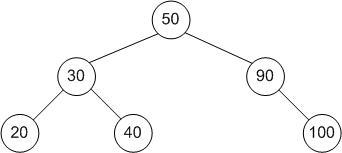
\includegraphics[width=1.0\linewidth,height=6.5in,keepaspectratio]{../images/25.jpg}
\end{center}
\raggedright{}\myfigurewithoutcaption{25}
\end{minipage}\vspace{0.75cm}


\\

\TemplateSpaceIndent{$\text{ }${}{\bfseries \setmainfont[Path=/usr/share/fonts/truetype/cmu/,UprightFont=cmunrm.ttf,BoldFont=cmunbx.ttf,ItalicFont=cmunti.ttf,BoldItalicFont=cmunbi.ttf]{cmunbx.ttf}\setmonofont[Path=/usr/share/fonts/truetype/cmu/,UprightFont=cmuntt.ttf,BoldFont=cmuntb.ttf,ItalicFont=cmunit.ttf,BoldItalicFont=cmuntx.ttf]{cmunbx.ttf}\bfseries preorder:} $\text{ }${}$\text{ }${}\setmainfont[Path=/usr/share/fonts/truetype/cmu/,UprightFont=cmunrm.ttf,BoldFont=cmunbx.ttf,ItalicFont=cmunti.ttf,BoldItalicFont=cmunbi.ttf]{cmunrm.ttf}\setmonofont[Path=/usr/share/fonts/truetype/cmu/,UprightFont=cmuntt.ttf,BoldFont=cmuntb.ttf,ItalicFont=cmunit.ttf,BoldItalicFont=cmuntx.ttf]{cmunrm.ttf}50,30,$\text{ }${}20,$\text{ }${}40,$\text{ }${}90,$\text{ }${}100$\text{ }$\newline{}
$\text{ }${}{\bfseries \setmainfont[Path=/usr/share/fonts/truetype/cmu/,UprightFont=cmunrm.ttf,BoldFont=cmunbx.ttf,ItalicFont=cmunti.ttf,BoldItalicFont=cmunbi.ttf]{cmunbx.ttf}\setmonofont[Path=/usr/share/fonts/truetype/cmu/,UprightFont=cmuntt.ttf,BoldFont=cmuntb.ttf,ItalicFont=cmunit.ttf,BoldItalicFont=cmuntx.ttf]{cmunbx.ttf}\bfseries inorder:} $\text{ }${}\setmainfont[Path=/usr/share/fonts/truetype/cmu/,UprightFont=cmunrm.ttf,BoldFont=cmunbx.ttf,ItalicFont=cmunti.ttf,BoldItalicFont=cmunbi.ttf]{cmunrm.ttf}\setmonofont[Path=/usr/share/fonts/truetype/cmu/,UprightFont=cmuntt.ttf,BoldFont=cmuntb.ttf,ItalicFont=cmunit.ttf,BoldItalicFont=cmuntx.ttf]{cmunrm.ttf}20,30,40,50,$\text{ }${}90,$\text{ }${}100}

\subsection{Balancing}
\label{75}
When entries that are already {\itshape sorted} \setmainfont[Path=/usr/share/fonts/truetype/cmu/,UprightFont=cmunrm.ttf,BoldFont=cmunbx.ttf,ItalicFont=cmunti.ttf,BoldItalicFont=cmunbi.ttf]{cmunrm.ttf}\setmonofont[Path=/usr/share/fonts/truetype/cmu/,UprightFont=cmuntt.ttf,BoldFont=cmuntb.ttf,ItalicFont=cmunit.ttf,BoldItalicFont=cmuntx.ttf]{cmunrm.ttf} are stored in a tree, all new records will go the same route, and the tree will look more like a list (such a tree is called a degenerate tree). Therefore the tree needs balancing routines, making sure that under all branches are an equal number of records. This will keep searching in the tree at optimal speed.  Specifically, if a tree with {\itshape n} \setmainfont[Path=/usr/share/fonts/truetype/cmu/,UprightFont=cmunrm.ttf,BoldFont=cmunbx.ttf,ItalicFont=cmunti.ttf,BoldItalicFont=cmunbi.ttf]{cmunrm.ttf}\setmonofont[Path=/usr/share/fonts/truetype/cmu/,UprightFont=cmuntt.ttf,BoldFont=cmuntb.ttf,ItalicFont=cmunit.ttf,BoldItalicFont=cmuntx.ttf]{cmunrm.ttf} nodes is a degenerate tree, the longest path through the tree will be n nodes; if it is a balanced tree, the longest path will be {\itshape log n} \setmainfont[Path=/usr/share/fonts/truetype/cmu/,UprightFont=cmunrm.ttf,BoldFont=cmunbx.ttf,ItalicFont=cmunti.ttf,BoldItalicFont=cmunbi.ttf]{cmunrm.ttf}\setmonofont[Path=/usr/share/fonts/truetype/cmu/,UprightFont=cmuntt.ttf,BoldFont=cmuntb.ttf,ItalicFont=cmunit.ttf,BoldItalicFont=cmuntx.ttf]{cmunrm.ttf} nodes.

\myhref{http://en.wikibooks.org/wiki/Algorithms\%2FLeft_rotation}{Algorithms/Left\_rotation}: This shows how balancing is applied to establish a priority heap invariant in  a \myhref{http://en.wikipedia.org/wiki/Treap}{Treap}, a data structure which has the queueing performance of a heap, and the key lookup performance of a tree. A balancing operation can change the tree structure while maintaining another order, which is binary tree sort order. The binary tree order is left to right, with left nodes\textquotesingle{} keys less than right nodes\textquotesingle{} keys, whereas the priority order is up and down, with higher nodes\textquotesingle{} priorities greater than lower nodes\textquotesingle{} priorities. Alternatively, the priority can be viewed as another ordering key, except that finding a specific key is more involved. 

The balancing operation can move nodes up and down a tree without affecting the left right ordering.


{\bfseries \myhref{http://en.wikipedia.org/wiki/AVL_tree}{\setmainfont[Path=/usr/share/fonts/truetype/cmu/,UprightFont=cmunrm.ttf,BoldFont=cmunbx.ttf,ItalicFont=cmunti.ttf,BoldItalicFont=cmunbi.ttf]{cmunbx.ttf}\setmonofont[Path=/usr/share/fonts/truetype/cmu/,UprightFont=cmuntt.ttf,BoldFont=cmuntb.ttf,ItalicFont=cmunit.ttf,BoldItalicFont=cmuntx.ttf]{cmunbx.ttf}\bfseries AVL}\setmainfont[Path=/usr/share/fonts/truetype/cmu/,UprightFont=cmunrm.ttf,BoldFont=cmunbx.ttf,ItalicFont=cmunti.ttf,BoldItalicFont=cmunbi.ttf]{cmunbx.ttf}\setmonofont[Path=/usr/share/fonts/truetype/cmu/,UprightFont=cmuntt.ttf,BoldFont=cmuntb.ttf,ItalicFont=cmunit.ttf,BoldItalicFont=cmuntx.ttf]{cmunbx.ttf}\bfseries :} \setmainfont[Path=/usr/share/fonts/truetype/cmu/,UprightFont=cmunrm.ttf,BoldFont=cmunbx.ttf,ItalicFont=cmunti.ttf,BoldItalicFont=cmunbi.ttf]{cmunrm.ttf}\setmonofont[Path=/usr/share/fonts/truetype/cmu/,UprightFont=cmuntt.ttf,BoldFont=cmuntb.ttf,ItalicFont=cmunit.ttf,BoldItalicFont=cmuntx.ttf]{cmunrm.ttf} A balanced binary search tree according to the following specification: the heights of the two child subtrees of any node differ by at most one.

{\bfseries \myhref{http://en.wikipedia.org/wiki/Red_black_tree}{\setmainfont[Path=/usr/share/fonts/truetype/cmu/,UprightFont=cmunrm.ttf,BoldFont=cmunbx.ttf,ItalicFont=cmunti.ttf,BoldItalicFont=cmunbi.ttf]{cmunbx.ttf}\setmonofont[Path=/usr/share/fonts/truetype/cmu/,UprightFont=cmuntt.ttf,BoldFont=cmuntb.ttf,ItalicFont=cmunit.ttf,BoldItalicFont=cmuntx.ttf]{cmunbx.ttf}\bfseries Red-{}Black Tree}\setmainfont[Path=/usr/share/fonts/truetype/cmu/,UprightFont=cmunrm.ttf,BoldFont=cmunbx.ttf,ItalicFont=cmunti.ttf,BoldItalicFont=cmunbi.ttf]{cmunbx.ttf}\setmonofont[Path=/usr/share/fonts/truetype/cmu/,UprightFont=cmuntt.ttf,BoldFont=cmuntb.ttf,ItalicFont=cmunit.ttf,BoldItalicFont=cmuntx.ttf]{cmunbx.ttf}\bfseries :} \setmainfont[Path=/usr/share/fonts/truetype/cmu/,UprightFont=cmunrm.ttf,BoldFont=cmunbx.ttf,ItalicFont=cmunti.ttf,BoldItalicFont=cmunbi.ttf]{cmunrm.ttf}\setmonofont[Path=/usr/share/fonts/truetype/cmu/,UprightFont=cmuntt.ttf,BoldFont=cmuntb.ttf,ItalicFont=cmunit.ttf,BoldItalicFont=cmuntx.ttf]{cmunrm.ttf} A balanced binary search tree using a balancing algorithm based on colors assigned to a node, and the colors of nearby nodes.

{\bfseries \setmainfont[Path=/usr/share/fonts/truetype/cmu/,UprightFont=cmunrm.ttf,BoldFont=cmunbx.ttf,ItalicFont=cmunti.ttf,BoldItalicFont=cmunbi.ttf]{cmunbx.ttf}\setmonofont[Path=/usr/share/fonts/truetype/cmu/,UprightFont=cmuntt.ttf,BoldFont=cmuntb.ttf,ItalicFont=cmunit.ttf,BoldItalicFont=cmuntx.ttf]{cmunbx.ttf}\bfseries  \myhref{http://en.wikipedia.org/wiki/AA_tree}{AA Tree}:} \setmainfont[Path=/usr/share/fonts/truetype/cmu/,UprightFont=cmunrm.ttf,BoldFont=cmunbx.ttf,ItalicFont=cmunti.ttf,BoldItalicFont=cmunbi.ttf]{cmunrm.ttf}\setmonofont[Path=/usr/share/fonts/truetype/cmu/,UprightFont=cmuntt.ttf,BoldFont=cmuntb.ttf,ItalicFont=cmunit.ttf,BoldItalicFont=cmuntx.ttf]{cmunrm.ttf} A balanced tree, in fact a more restrictive variation of a red-{}black tree.
\subsection{Binary Search Trees}
\label{76}
A typical binary search tree looks like this:



\begin{minipage}{1.0\linewidth}
\begin{center}
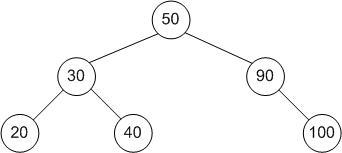
\includegraphics[width=1.0\linewidth,height=6.5in,keepaspectratio]{../images/26.jpg}
\end{center}
\raggedright{}\myfigurewithoutcaption{26}
\end{minipage}\vspace{0.75cm}


\subsubsection{Terms}
\label{77}
{\bfseries \setmainfont[Path=/usr/share/fonts/truetype/cmu/,UprightFont=cmunrm.ttf,BoldFont=cmunbx.ttf,ItalicFont=cmunti.ttf,BoldItalicFont=cmunbi.ttf]{cmunbx.ttf}\setmonofont[Path=/usr/share/fonts/truetype/cmu/,UprightFont=cmuntt.ttf,BoldFont=cmuntb.ttf,ItalicFont=cmunit.ttf,BoldItalicFont=cmuntx.ttf]{cmunbx.ttf}\bfseries Node} \setmainfont[Path=/usr/share/fonts/truetype/cmu/,UprightFont=cmunrm.ttf,BoldFont=cmunbx.ttf,ItalicFont=cmunti.ttf,BoldItalicFont=cmunbi.ttf]{cmunrm.ttf}\setmonofont[Path=/usr/share/fonts/truetype/cmu/,UprightFont=cmuntt.ttf,BoldFont=cmuntb.ttf,ItalicFont=cmunit.ttf,BoldItalicFont=cmuntx.ttf]{cmunrm.ttf} Any item that is stored in the tree.
{\bfseries \setmainfont[Path=/usr/share/fonts/truetype/cmu/,UprightFont=cmunrm.ttf,BoldFont=cmunbx.ttf,ItalicFont=cmunti.ttf,BoldItalicFont=cmunbi.ttf]{cmunbx.ttf}\setmonofont[Path=/usr/share/fonts/truetype/cmu/,UprightFont=cmuntt.ttf,BoldFont=cmuntb.ttf,ItalicFont=cmunit.ttf,BoldItalicFont=cmuntx.ttf]{cmunbx.ttf}\bfseries Root} \setmainfont[Path=/usr/share/fonts/truetype/cmu/,UprightFont=cmunrm.ttf,BoldFont=cmunbx.ttf,ItalicFont=cmunti.ttf,BoldItalicFont=cmunbi.ttf]{cmunrm.ttf}\setmonofont[Path=/usr/share/fonts/truetype/cmu/,UprightFont=cmuntt.ttf,BoldFont=cmuntb.ttf,ItalicFont=cmunit.ttf,BoldItalicFont=cmuntx.ttf]{cmunrm.ttf} The top item in the tree. (50 in the tree above)
{\bfseries \setmainfont[Path=/usr/share/fonts/truetype/cmu/,UprightFont=cmunrm.ttf,BoldFont=cmunbx.ttf,ItalicFont=cmunti.ttf,BoldItalicFont=cmunbi.ttf]{cmunbx.ttf}\setmonofont[Path=/usr/share/fonts/truetype/cmu/,UprightFont=cmuntt.ttf,BoldFont=cmuntb.ttf,ItalicFont=cmunit.ttf,BoldItalicFont=cmuntx.ttf]{cmunbx.ttf}\bfseries Child} \setmainfont[Path=/usr/share/fonts/truetype/cmu/,UprightFont=cmunrm.ttf,BoldFont=cmunbx.ttf,ItalicFont=cmunti.ttf,BoldItalicFont=cmunbi.ttf]{cmunrm.ttf}\setmonofont[Path=/usr/share/fonts/truetype/cmu/,UprightFont=cmuntt.ttf,BoldFont=cmuntb.ttf,ItalicFont=cmunit.ttf,BoldItalicFont=cmuntx.ttf]{cmunrm.ttf} Node(s) under the current node. (20 and 40 are children of 30 in the tree above)
{\bfseries \setmainfont[Path=/usr/share/fonts/truetype/cmu/,UprightFont=cmunrm.ttf,BoldFont=cmunbx.ttf,ItalicFont=cmunti.ttf,BoldItalicFont=cmunbi.ttf]{cmunbx.ttf}\setmonofont[Path=/usr/share/fonts/truetype/cmu/,UprightFont=cmuntt.ttf,BoldFont=cmuntb.ttf,ItalicFont=cmunit.ttf,BoldItalicFont=cmuntx.ttf]{cmunbx.ttf}\bfseries Parent} \setmainfont[Path=/usr/share/fonts/truetype/cmu/,UprightFont=cmunrm.ttf,BoldFont=cmunbx.ttf,ItalicFont=cmunti.ttf,BoldItalicFont=cmunbi.ttf]{cmunrm.ttf}\setmonofont[Path=/usr/share/fonts/truetype/cmu/,UprightFont=cmuntt.ttf,BoldFont=cmuntb.ttf,ItalicFont=cmunit.ttf,BoldItalicFont=cmuntx.ttf]{cmunrm.ttf} The node directly above the current node. (90 is the parent of 100 in the tree above)
{\bfseries \setmainfont[Path=/usr/share/fonts/truetype/cmu/,UprightFont=cmunrm.ttf,BoldFont=cmunbx.ttf,ItalicFont=cmunti.ttf,BoldItalicFont=cmunbi.ttf]{cmunbx.ttf}\setmonofont[Path=/usr/share/fonts/truetype/cmu/,UprightFont=cmuntt.ttf,BoldFont=cmuntb.ttf,ItalicFont=cmunit.ttf,BoldItalicFont=cmuntx.ttf]{cmunbx.ttf}\bfseries Leaf} \setmainfont[Path=/usr/share/fonts/truetype/cmu/,UprightFont=cmunrm.ttf,BoldFont=cmunbx.ttf,ItalicFont=cmunti.ttf,BoldItalicFont=cmunbi.ttf]{cmunrm.ttf}\setmonofont[Path=/usr/share/fonts/truetype/cmu/,UprightFont=cmuntt.ttf,BoldFont=cmuntb.ttf,ItalicFont=cmunit.ttf,BoldItalicFont=cmuntx.ttf]{cmunrm.ttf} A node which has no children. (20 is a leaf in the tree above)
\subsubsection{Searching through a binary search tree}
\label{78}
To search for an item in a binary tree:

\begin{myenumerate}
\item{}  Start at the root node
\item{}  If the item that you are searching for is less than the root node, move to the left child of the root node, if the item that you are searching for is more than the root node, move to the right child of the root node and if it is equal to the root node, then you have found the item that you are looking for.
\item{}  Now check to see if the item that you are searching for is equal to, less than or more than the new node that you are on.  Again if the item that you are searching for is less than the current node, move to the left child, and if the item that you are searching for is greater than the current node, move to the right child.
\item{}  Repeat this process until you find the item that you are looking for or until the node does not have a child on the correct branch, in which case the tree doesn\textquotesingle{}t contain the item which you are looking for.
\end{myenumerate}

\paragraph{Example}
{$\text{ }$}\newline\label{79}


\begin{minipage}{1.0\linewidth}
\begin{center}
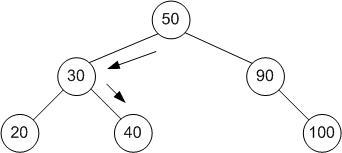
\includegraphics[width=1.0\linewidth,height=6.5in,keepaspectratio]{../images/27.jpg}
\end{center}
\raggedright{}\myfigurewithoutcaption{27}
\end{minipage}\vspace{0.75cm}



{\bfseries \setmainfont[Path=/usr/share/fonts/truetype/cmu/,UprightFont=cmunrm.ttf,BoldFont=cmunbx.ttf,ItalicFont=cmunti.ttf,BoldItalicFont=cmunbi.ttf]{cmunbx.ttf}\setmonofont[Path=/usr/share/fonts/truetype/cmu/,UprightFont=cmuntt.ttf,BoldFont=cmuntb.ttf,ItalicFont=cmunit.ttf,BoldItalicFont=cmuntx.ttf]{cmunbx.ttf}\bfseries For example, to find the node 40...} \setmainfont[Path=/usr/share/fonts/truetype/cmu/,UprightFont=cmunrm.ttf,BoldFont=cmunbx.ttf,ItalicFont=cmunti.ttf,BoldItalicFont=cmunbi.ttf]{cmunrm.ttf}\setmonofont[Path=/usr/share/fonts/truetype/cmu/,UprightFont=cmuntt.ttf,BoldFont=cmuntb.ttf,ItalicFont=cmunit.ttf,BoldItalicFont=cmuntx.ttf]{cmunrm.ttf}

\begin{myenumerate}
\item{}  The root node is 50, which is greater than 40, so you go to 50\textquotesingle{}s left child.
\item{}  50\textquotesingle{}s left child is 30, which is less than 40, so you next go to 30\textquotesingle{}s right child.
\item{}  30\textquotesingle{}s right child is 40, so you have found the item that you are looking for :)
\end{myenumerate}

.........
\subsubsection{Adding an item to a binary search tree}
\label{80}
\begin{myenumerate}
\item{}  To add an item, you first must search through the tree to find the position that you should put it in.  You do this following the steps above.
\item{}  When you reach a node which doesn\textquotesingle{}t contain a child on the correct branch, add the new node there.
\end{myenumerate}




{\bfseries \setmainfont[Path=/usr/share/fonts/truetype/cmu/,UprightFont=cmunrm.ttf,BoldFont=cmunbx.ttf,ItalicFont=cmunti.ttf,BoldItalicFont=cmunbi.ttf]{cmunbx.ttf}\setmonofont[Path=/usr/share/fonts/truetype/cmu/,UprightFont=cmuntt.ttf,BoldFont=cmuntb.ttf,ItalicFont=cmunit.ttf,BoldItalicFont=cmuntx.ttf]{cmunbx.ttf}\bfseries For example, to add the node 25...} \setmainfont[Path=/usr/share/fonts/truetype/cmu/,UprightFont=cmunrm.ttf,BoldFont=cmunbx.ttf,ItalicFont=cmunti.ttf,BoldItalicFont=cmunbi.ttf]{cmunrm.ttf}\setmonofont[Path=/usr/share/fonts/truetype/cmu/,UprightFont=cmuntt.ttf,BoldFont=cmuntb.ttf,ItalicFont=cmunit.ttf,BoldItalicFont=cmuntx.ttf]{cmunrm.ttf}

\begin{myenumerate}
\item{}  The root node is 50, which is greater than 25, so you go to 50\textquotesingle{}s left child.
\item{}  50\textquotesingle{}s left child is 30, which is greater than 25, so you go to 30\textquotesingle{}s left child.
\item{}  30\textquotesingle{}s left child is 20, which is less than 25, so you go to 20\textquotesingle{}s right child.
\item{}  20\textquotesingle{}s right child doesn\textquotesingle{}t exist, so you add 25 there :)
\end{myenumerate}

\subsubsection{Deleting an item from a binary search tree}
\label{81}
{\itshape It is assumed that you have already found the node that you want to delete, using the search technique described above.} \setmainfont[Path=/usr/share/fonts/truetype/cmu/,UprightFont=cmunrm.ttf,BoldFont=cmunbx.ttf,ItalicFont=cmunti.ttf,BoldItalicFont=cmunbi.ttf]{cmunrm.ttf}\setmonofont[Path=/usr/share/fonts/truetype/cmu/,UprightFont=cmuntt.ttf,BoldFont=cmuntb.ttf,ItalicFont=cmunit.ttf,BoldItalicFont=cmuntx.ttf]{cmunrm.ttf}
\paragraph{Case 1: The node you want to delete is a leaf}
{$\text{ }$}\newline\label{82}


\begin{minipage}{1.0\linewidth}
\begin{center}
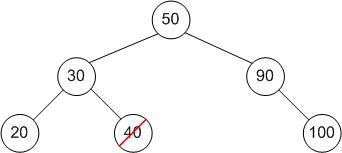
\includegraphics[width=1.0\linewidth,height=6.5in,keepaspectratio]{../images/28.jpg}
\end{center}
\raggedright{}\myfigurewithoutcaption{28}
\end{minipage}\vspace{0.75cm}



{\bfseries \setmainfont[Path=/usr/share/fonts/truetype/cmu/,UprightFont=cmunrm.ttf,BoldFont=cmunbx.ttf,ItalicFont=cmunti.ttf,BoldItalicFont=cmunbi.ttf]{cmunbx.ttf}\setmonofont[Path=/usr/share/fonts/truetype/cmu/,UprightFont=cmuntt.ttf,BoldFont=cmuntb.ttf,ItalicFont=cmunit.ttf,BoldItalicFont=cmuntx.ttf]{cmunbx.ttf}\bfseries For example, to delete 40...} \setmainfont[Path=/usr/share/fonts/truetype/cmu/,UprightFont=cmunrm.ttf,BoldFont=cmunbx.ttf,ItalicFont=cmunti.ttf,BoldItalicFont=cmunbi.ttf]{cmunrm.ttf}\setmonofont[Path=/usr/share/fonts/truetype/cmu/,UprightFont=cmuntt.ttf,BoldFont=cmuntb.ttf,ItalicFont=cmunit.ttf,BoldItalicFont=cmuntx.ttf]{cmunrm.ttf}

\begin{myitemize}
\item{}  Simply delete the node!
\end{myitemize}

\paragraph{Case 2: The node you want to delete has one child}
{$\text{ }$}\newline\label{83}
\begin{myenumerate}
\item{}  Directly connect the child of the node that you want to delete, to the parent of the node that you want to delete.
\end{myenumerate}




\begin{minipage}{1.0\linewidth}
\begin{center}
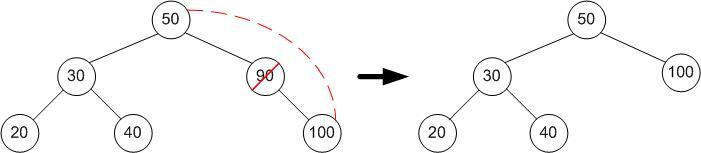
\includegraphics[width=1.0\linewidth,height=6.5in,keepaspectratio]{../images/29.jpg}
\end{center}
\raggedright{}\myfigurewithoutcaption{29}
\end{minipage}\vspace{0.75cm}



{\bfseries \setmainfont[Path=/usr/share/fonts/truetype/cmu/,UprightFont=cmunrm.ttf,BoldFont=cmunbx.ttf,ItalicFont=cmunti.ttf,BoldItalicFont=cmunbi.ttf]{cmunbx.ttf}\setmonofont[Path=/usr/share/fonts/truetype/cmu/,UprightFont=cmuntt.ttf,BoldFont=cmuntb.ttf,ItalicFont=cmunit.ttf,BoldItalicFont=cmuntx.ttf]{cmunbx.ttf}\bfseries For example, to delete 90...} \setmainfont[Path=/usr/share/fonts/truetype/cmu/,UprightFont=cmunrm.ttf,BoldFont=cmunbx.ttf,ItalicFont=cmunti.ttf,BoldItalicFont=cmunbi.ttf]{cmunrm.ttf}\setmonofont[Path=/usr/share/fonts/truetype/cmu/,UprightFont=cmuntt.ttf,BoldFont=cmuntb.ttf,ItalicFont=cmunit.ttf,BoldItalicFont=cmuntx.ttf]{cmunrm.ttf}

\begin{myitemize}
\item{}  Delete 90, then make 100 the child node of 50.
\end{myitemize}

\paragraph{Case 3: The node you want to delete has two children}
{$\text{ }$}\newline\label{84}
One {\itshape non-{}standard} \setmainfont[Path=/usr/share/fonts/truetype/cmu/,UprightFont=cmunrm.ttf,BoldFont=cmunbx.ttf,ItalicFont=cmunti.ttf,BoldItalicFont=cmunbi.ttf]{cmunrm.ttf}\setmonofont[Path=/usr/share/fonts/truetype/cmu/,UprightFont=cmuntt.ttf,BoldFont=cmuntb.ttf,ItalicFont=cmunit.ttf,BoldItalicFont=cmuntx.ttf]{cmunrm.ttf} way, is to \uline{rotate} the node into a chosen subtree, and attempt to delete the key again from that subtree, recursively, until Case 1 or Case 2 occurs. This
could unbalance a tree, so randomly choosing whether to right or left rotate may help.

The {\itshape standard} \setmainfont[Path=/usr/share/fonts/truetype/cmu/,UprightFont=cmunrm.ttf,BoldFont=cmunbx.ttf,ItalicFont=cmunti.ttf,BoldItalicFont=cmunbi.ttf]{cmunrm.ttf}\setmonofont[Path=/usr/share/fonts/truetype/cmu/,UprightFont=cmuntt.ttf,BoldFont=cmuntb.ttf,ItalicFont=cmunit.ttf,BoldItalicFont=cmuntx.ttf]{cmunrm.ttf} way is to pick either the left or right child, say the right, then get the right\textquotesingle{}s leftmost descendent by following left ,starting from the right child, until the next left is null. Then remove this leftmost descendant of the right child, replacing it with its right sub-{}tree ( it has a left child of null). Then use the contents of this former leftmost descendant of the right child,   as replacement for the key and value of the node being deleted , so that its values now are in the deleted node, the parent of the right child. 
This still maintains the key ordering for all nodes. Example java code is below in the treap example code. 

The following examples use the standard algorithm, that is, the successor is the left-{}most node in the right subtree of the node to be deleted.



\begin{minipage}{1.0\linewidth}
\begin{center}
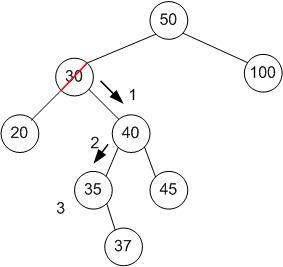
\includegraphics[width=1.0\linewidth,height=6.5in,keepaspectratio]{../images/30.jpg}
\end{center}
\raggedright{}\myfigurewithoutcaption{30}
\end{minipage}\vspace{0.75cm}



{\bfseries \setmainfont[Path=/usr/share/fonts/truetype/cmu/,UprightFont=cmunrm.ttf,BoldFont=cmunbx.ttf,ItalicFont=cmunti.ttf,BoldItalicFont=cmunbi.ttf]{cmunbx.ttf}\setmonofont[Path=/usr/share/fonts/truetype/cmu/,UprightFont=cmuntt.ttf,BoldFont=cmuntb.ttf,ItalicFont=cmunit.ttf,BoldItalicFont=cmuntx.ttf]{cmunbx.ttf}\bfseries For example, to delete 30} \setmainfont[Path=/usr/share/fonts/truetype/cmu/,UprightFont=cmunrm.ttf,BoldFont=cmunbx.ttf,ItalicFont=cmunti.ttf,BoldItalicFont=cmunbi.ttf]{cmunrm.ttf}\setmonofont[Path=/usr/share/fonts/truetype/cmu/,UprightFont=cmuntt.ttf,BoldFont=cmuntb.ttf,ItalicFont=cmunit.ttf,BoldItalicFont=cmuntx.ttf]{cmunrm.ttf}

\begin{myenumerate}
\item{}  The right node of the node which is being deleted is 40.
\item{}  (From now on, we continually go to the left node until there isn\textquotesingle{}t another one...) The first left node of 40, is 35.
\item{}  35 has no left node, therefore 35 is the successor!
\item{}  35 replaces 30, at the original right node, and the node with 35 is deleted, replacing it with the right sub-{}tree, which has the root node 37.
\end{myenumerate}

\subparagraph{Case 1 of two-{}children case: The successor is the right child of the node being deleted}
{$\text{ }$}\newline\label{85}

\begin{myenumerate}
\item{}  Directly move the child to the right of the node being deleted into the position of the node being deleted.
\item{}  As the new node has no left children, you can connect the deleted node\textquotesingle{}s left subtree\textquotesingle{}s root as it\textquotesingle{}s left child.
\end{myenumerate}




\begin{minipage}{1.0\linewidth}
\begin{center}
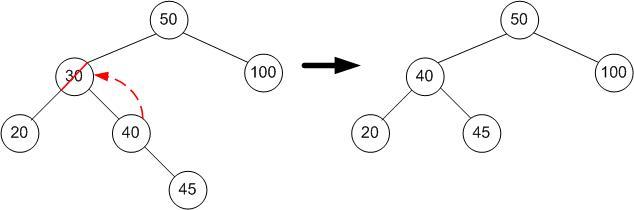
\includegraphics[width=1.0\linewidth,height=6.5in,keepaspectratio]{../images/31.jpg}
\end{center}
\raggedright{}\myfigurewithoutcaption{31}
\end{minipage}\vspace{0.75cm}



{\bfseries \setmainfont[Path=/usr/share/fonts/truetype/cmu/,UprightFont=cmunrm.ttf,BoldFont=cmunbx.ttf,ItalicFont=cmunti.ttf,BoldItalicFont=cmunbi.ttf]{cmunbx.ttf}\setmonofont[Path=/usr/share/fonts/truetype/cmu/,UprightFont=cmuntt.ttf,BoldFont=cmuntb.ttf,ItalicFont=cmunit.ttf,BoldItalicFont=cmuntx.ttf]{cmunbx.ttf}\bfseries For example, to delete 30} \setmainfont[Path=/usr/share/fonts/truetype/cmu/,UprightFont=cmunrm.ttf,BoldFont=cmunbx.ttf,ItalicFont=cmunti.ttf,BoldItalicFont=cmunbi.ttf]{cmunrm.ttf}\setmonofont[Path=/usr/share/fonts/truetype/cmu/,UprightFont=cmuntt.ttf,BoldFont=cmuntb.ttf,ItalicFont=cmunit.ttf,BoldItalicFont=cmuntx.ttf]{cmunrm.ttf}

\begin{myenumerate}
\item{}  replace the contents to be deleted (30), with the successor\textquotesingle{}s contents( 40).
\item{}  delete the successor node (contents 40), replacing it with its right subtree (head contents 45).
\end{myenumerate}

\subparagraph{Case 2 of two-{}children case: The successor isn\textquotesingle{}t the right child of the node being deleted}
{$\text{ }$}\newline\label{86}
{\itshape This is best shown with an example} \setmainfont[Path=/usr/share/fonts/truetype/cmu/,UprightFont=cmunrm.ttf,BoldFont=cmunbx.ttf,ItalicFont=cmunti.ttf,BoldItalicFont=cmunbi.ttf]{cmunrm.ttf}\setmonofont[Path=/usr/share/fonts/truetype/cmu/,UprightFont=cmuntt.ttf,BoldFont=cmuntb.ttf,ItalicFont=cmunit.ttf,BoldItalicFont=cmuntx.ttf]{cmunrm.ttf}



\begin{minipage}{1.0\linewidth}
\begin{center}
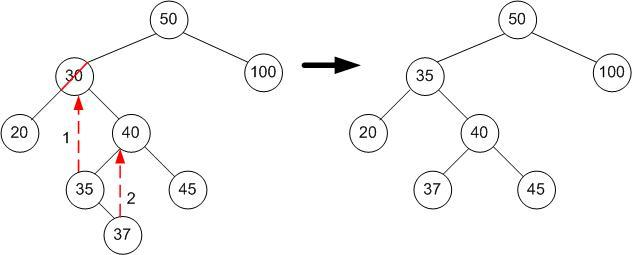
\includegraphics[width=1.0\linewidth,height=6.5in,keepaspectratio]{../images/32.jpg}
\end{center}
\raggedright{}\myfigurewithoutcaption{32}
\end{minipage}\vspace{0.75cm}



{\bfseries \setmainfont[Path=/usr/share/fonts/truetype/cmu/,UprightFont=cmunrm.ttf,BoldFont=cmunbx.ttf,ItalicFont=cmunti.ttf,BoldItalicFont=cmunbi.ttf]{cmunbx.ttf}\setmonofont[Path=/usr/share/fonts/truetype/cmu/,UprightFont=cmuntt.ttf,BoldFont=cmuntb.ttf,ItalicFont=cmunit.ttf,BoldItalicFont=cmuntx.ttf]{cmunbx.ttf}\bfseries To delete 30...} \setmainfont[Path=/usr/share/fonts/truetype/cmu/,UprightFont=cmunrm.ttf,BoldFont=cmunbx.ttf,ItalicFont=cmunti.ttf,BoldItalicFont=cmunbi.ttf]{cmunrm.ttf}\setmonofont[Path=/usr/share/fonts/truetype/cmu/,UprightFont=cmuntt.ttf,BoldFont=cmuntb.ttf,ItalicFont=cmunit.ttf,BoldItalicFont=cmuntx.ttf]{cmunrm.ttf}

\begin{myenumerate}
\item{}  Replace the  contents to be deleted (30) with the successor\textquotesingle{}s contents (35).
\item{}  replace the successor (35) with it\textquotesingle{}s right subtree (37). There is no left subtree because the successor is leftmost.
\end{myenumerate}

\subsection{Example extract of java code for binary tree delete operation}
\label{87}

\begin{Shaded}
\begin{Highlighting}[]

\KeywordTok{private}\ensuremath{\text{ }}\NormalTok{Treap1<K,\ensuremath{\text{ }}V>.}\FunctionTok{TreapNode}\ensuremath{\text{ }}\FunctionTok{deleteNode}\NormalTok{(K\ensuremath{\text{ }}k,\ensuremath{\text{ }}Treap1<K,\ensuremath{\text{ }}V>.}\FunctionTok{TreapNode}\ensuremath{\text{ }}\NormalTok{node,}\newline
\ensuremath{\text{ }}\NormalTok{Deleted\ensuremath{\text{ }}del)\ensuremath{\text{ }}\{}\newline
\ensuremath{\text{ }}\newline
		\KeywordTok{if}\ensuremath{\text{ }}\NormalTok{(node\ensuremath{\text{ }}==\ensuremath{\text{ }}}\KeywordTok{null}\NormalTok{)\ensuremath{\text{ }}\{}\newline
			\KeywordTok{return}\ensuremath{\text{ }}\KeywordTok{null}\NormalTok{;}\newline
		\NormalTok{\}\ensuremath{\text{ }}}\KeywordTok{else}\ensuremath{\text{ }}\KeywordTok{if}\ensuremath{\text{ }}\NormalTok{(k.}\FunctionTok{compareTo}\NormalTok{(node.}\FunctionTok{k}\NormalTok{)\ensuremath{\text{ }}<\ensuremath{\text{ }}}\DecValTok{0}\NormalTok{)\ensuremath{\text{ }}\{}\newline
			\ensuremath{\text{ }}\NormalTok{node.}\FunctionTok{left}\ensuremath{\text{ }}\NormalTok{=\ensuremath{\text{ }}}\FunctionTok{deleteNode}\NormalTok{(k,\ensuremath{\text{ }}node.}\FunctionTok{left}\NormalTok{,\ensuremath{\text{ }}del)\ensuremath{\text{ }};}\newline
		\NormalTok{\}\ensuremath{\text{ }}}\KeywordTok{else}\ensuremath{\text{ }}\KeywordTok{if}\ensuremath{\text{ }}\NormalTok{(k.}\FunctionTok{compareTo}\NormalTok{(node.}\FunctionTok{k}\NormalTok{)\ensuremath{\text{ }}>\ensuremath{\text{ }}}\DecValTok{0}\NormalTok{)\ensuremath{\text{ }}\{}\newline
			\NormalTok{node.}\FunctionTok{right}\ensuremath{\text{ }}\NormalTok{=\ensuremath{\text{ }}\ensuremath{\text{ }}}\FunctionTok{deleteNode}\NormalTok{(k,\ensuremath{\text{ }}node.}\FunctionTok{right}\NormalTok{,\ensuremath{\text{ }}del);}\newline
\ensuremath{\text{ }}\newline
			\CommentTok{//\ensuremath{\text{ }}k.compareTo(node.k)\ensuremath{\text{ }}==\ensuremath{\text{ }}0}\newline
		\NormalTok{\}\ensuremath{\text{ }}}\KeywordTok{else}\ensuremath{\text{ }}\KeywordTok{if}\ensuremath{\text{ }}\NormalTok{(\ensuremath{\text{ }}node.}\FunctionTok{left}\ensuremath{\text{ }}\NormalTok{==\ensuremath{\text{ }}}\KeywordTok{null}\ensuremath{\text{ }}\NormalTok{)\ensuremath{\text{ }}\{}\newline
				\NormalTok{del.}\FunctionTok{success}\ensuremath{\text{ }}\NormalTok{=\ensuremath{\text{ }}}\KeywordTok{true}\NormalTok{;}\newline
				\KeywordTok{return}\ensuremath{\text{ }}\NormalTok{node.}\FunctionTok{right}\NormalTok{;}\newline
		\NormalTok{\}\ensuremath{\text{ }}}\KeywordTok{else}\ensuremath{\text{ }}\KeywordTok{if}\ensuremath{\text{ }}\NormalTok{(\ensuremath{\text{ }}node.}\FunctionTok{right}\ensuremath{\text{ }}\NormalTok{==\ensuremath{\text{ }}}\KeywordTok{null}\NormalTok{)\ensuremath{\text{ }}\{}\newline
			\ensuremath{\text{ }}\ensuremath{\text{ }}\ensuremath{\text{ }}\ensuremath{\text{ }}\NormalTok{del.}\FunctionTok{success}\ensuremath{\text{ }}\NormalTok{=\ensuremath{\text{ }}}\KeywordTok{true}\NormalTok{;}\newline
				\KeywordTok{return}\ensuremath{\text{ }}\ensuremath{\text{ }}\NormalTok{node.}\FunctionTok{left}\NormalTok{;}\newline
		\NormalTok{\}\ensuremath{\text{ }}}\KeywordTok{else}\ensuremath{\text{ }}\ensuremath{\text{ }}\KeywordTok{if}\ensuremath{\text{ }}\NormalTok{(node.}\FunctionTok{left}\ensuremath{\text{ }}\NormalTok{!=}\KeywordTok{null}\ensuremath{\text{ }}\NormalTok{\&\&\ensuremath{\text{ }}node.}\FunctionTok{right}\ensuremath{\text{ }}\NormalTok{!=\ensuremath{\text{ }}}\KeywordTok{null}\NormalTok{)\{}\newline
		\CommentTok{/*}\newline
\CommentTok{\ensuremath{\text{ }}\ensuremath{\text{ }}\ensuremath{\text{ }}\ensuremath{\text{ }}\ensuremath{\text{ }}\ensuremath{\text{ }}\ensuremath{\text{ }}\ensuremath{\text{ }}\ensuremath{\text{ }}\ensuremath{\text{ }}\ensuremath{\text{ }}\ensuremath{\text{ }}\ensuremath{\text{ }}\ensuremath{\text{ }}\ensuremath{\text{ }}\ensuremath{\text{ }}//\ensuremath{\text{ }}\ensuremath{\text{ }}non-standard\ensuremath{\text{ }}method,}\newline
\CommentTok{		//\ensuremath{\text{ }}left\ensuremath{\text{ }}rotate\ensuremath{\text{ }}and\ensuremath{\text{ }}all\ensuremath{\text{ }}delete\ensuremath{\text{ }}on\ensuremath{\text{ }}left\ensuremath{\text{ }}subtree}\newline
\CommentTok{\ensuremath{\text{ }}}\newline
\CommentTok{			TreapNode\ensuremath{\text{ }}tmp\ensuremath{\text{ }}=\ensuremath{\text{ }}node.right;}\newline
\CommentTok{			node.right\ensuremath{\text{ }}=\ensuremath{\text{ }}node.right.left;}\newline
\CommentTok{		\ensuremath{\text{ }}\ensuremath{\text{ }}\ensuremath{\text{ }}\ensuremath{\text{ }}\ensuremath{\text{ }}\ensuremath{\text{ }}\ensuremath{\text{ }}\ensuremath{\text{ }}tmp.left\ensuremath{\text{ }}=\ensuremath{\text{ }}node;}\newline
\CommentTok{		\ensuremath{\text{ }}\ensuremath{\text{ }}\ensuremath{\text{ }}\ensuremath{\text{ }}\ensuremath{\text{ }}\ensuremath{\text{ }}\ensuremath{\text{ }}\ensuremath{\text{ }}node\ensuremath{\text{ }}=\ensuremath{\text{ }}tmp;			}\newline
\CommentTok{			node.left\ensuremath{\text{ }}=\ensuremath{\text{ }}deleteNode(k\ensuremath{\text{ }},\ensuremath{\text{ }}node.left,\ensuremath{\text{ }}del);}\newline
\CommentTok{			}\newline
\CommentTok{\ensuremath{\text{ }}\ensuremath{\text{ }}\ensuremath{\text{ }}\ensuremath{\text{ }}\ensuremath{\text{ }}\ensuremath{\text{ }}\ensuremath{\text{ }}\ensuremath{\text{ }}\ensuremath{\text{ }}\ensuremath{\text{ }}\ensuremath{\text{ }}\ensuremath{\text{ }}\ensuremath{\text{ }}\ensuremath{\text{ }}\ensuremath{\text{ }}\ensuremath{\text{ }}\ensuremath{\text{ }}*/}\newline
\ensuremath{\text{ }}\newline
	\ensuremath{\text{ }}\ensuremath{\text{ }}\ensuremath{\text{ }}\ensuremath{\text{ }}\ensuremath{\text{ }}\ensuremath{\text{ }}\ensuremath{\text{ }}\ensuremath{\text{ }}\CommentTok{//\ensuremath{\text{ }}more\ensuremath{\text{ }}standard\ensuremath{\text{ }}method\ensuremath{\text{ }}?\ensuremath{\text{ }}doesn\textquotesingle{}t\ensuremath{\text{ }}disturb\ensuremath{\text{ }}tree\ensuremath{\text{ }}structure\ensuremath{\text{ }}as\ensuremath{\text{ }}much}\newline
	\ensuremath{\text{ }}\ensuremath{\text{ }}\ensuremath{\text{ }}\ensuremath{\text{ }}\ensuremath{\text{ }}\ensuremath{\text{ }}\ensuremath{\text{ }}\ensuremath{\text{ }}\CommentTok{//\ensuremath{\text{ }}find\ensuremath{\text{ }}leftmost\ensuremath{\text{ }}descendant\ensuremath{\text{ }}of\ensuremath{\text{ }}the\ensuremath{\text{ }}right\ensuremath{\text{ }}child\ensuremath{\text{ }}node\ensuremath{\text{ }}and\ensuremath{\text{ }}replace}\newline
\ensuremath{\text{ }}\NormalTok{contents}\newline
\ensuremath{\text{ }}\newline
			\NormalTok{TreapNode\ensuremath{\text{ }}n2\ensuremath{\text{ }}\ensuremath{\text{ }}=\ensuremath{\text{ }}node.}\FunctionTok{right}\NormalTok{;}\newline
			\NormalTok{TreapNode\ensuremath{\text{ }}previous2\ensuremath{\text{ }}=\ensuremath{\text{ }}}\KeywordTok{null}\NormalTok{;}\newline
			\KeywordTok{while}\ensuremath{\text{ }}\NormalTok{(n2.}\FunctionTok{left}\ensuremath{\text{ }}\NormalTok{!=\ensuremath{\text{ }}}\KeywordTok{null}\NormalTok{)\ensuremath{\text{ }}\{}\newline
				\NormalTok{previous2\ensuremath{\text{ }}=\ensuremath{\text{ }}n2;}\newline
				\NormalTok{n2\ensuremath{\text{ }}=\ensuremath{\text{ }}n2.}\FunctionTok{left}\NormalTok{;}\newline
			\NormalTok{\}}\newline
\ensuremath{\text{ }}\newline
			\KeywordTok{if}\ensuremath{\text{ }}\NormalTok{(previous2\ensuremath{\text{ }}!=\ensuremath{\text{ }}}\KeywordTok{null}\NormalTok{)\ensuremath{\text{ }}\{}\newline
				\NormalTok{previous2.}\FunctionTok{left}\ensuremath{\text{ }}\NormalTok{=\ensuremath{\text{ }}n2.}\FunctionTok{right}\NormalTok{;}\newline
\ensuremath{\text{ }}\ensuremath{\text{ }}\ensuremath{\text{ }}\ensuremath{\text{ }}\ensuremath{\text{ }}\ensuremath{\text{ }}\ensuremath{\text{ }}\ensuremath{\text{ }}\ensuremath{\text{ }}\ensuremath{\text{ }}\ensuremath{\text{ }}\ensuremath{\text{ }}\ensuremath{\text{ }}\ensuremath{\text{ }}\ensuremath{\text{ }}\ensuremath{\text{ }}\ensuremath{\text{ }}\ensuremath{\text{ }}\ensuremath{\text{ }}\ensuremath{\text{ }}\ensuremath{\text{ }}\ensuremath{\text{ }}\ensuremath{\text{ }}\ensuremath{\text{ }}\ensuremath{\text{ }}\ensuremath{\text{ }}\ensuremath{\text{ }}\ensuremath{\text{ }}\ensuremath{\text{ }}\ensuremath{\text{ }}\ensuremath{\text{ }}\ensuremath{\text{ }}\CommentTok{//n2\ensuremath{\text{ }}has\ensuremath{\text{ }}no\ensuremath{\text{ }}parent\ensuremath{\text{ }}link,\ensuremath{\text{ }}orphaned}\newline
			\NormalTok{\}\ensuremath{\text{ }}}\KeywordTok{else}\ensuremath{\text{ }}\NormalTok{\{}\newline
				\NormalTok{node.}\FunctionTok{right}\ensuremath{\text{ }}\NormalTok{=\ensuremath{\text{ }}n2.}\FunctionTok{right}\NormalTok{;}\newline
\ensuremath{\text{ }}\ensuremath{\text{ }}\ensuremath{\text{ }}\ensuremath{\text{ }}\ensuremath{\text{ }}\ensuremath{\text{ }}\ensuremath{\text{ }}\ensuremath{\text{ }}\ensuremath{\text{ }}\ensuremath{\text{ }}\ensuremath{\text{ }}\ensuremath{\text{ }}\ensuremath{\text{ }}\ensuremath{\text{ }}\ensuremath{\text{ }}\ensuremath{\text{ }}\ensuremath{\text{ }}\ensuremath{\text{ }}\ensuremath{\text{ }}\ensuremath{\text{ }}\ensuremath{\text{ }}\ensuremath{\text{ }}\ensuremath{\text{ }}\ensuremath{\text{ }}\ensuremath{\text{ }}\ensuremath{\text{ }}\ensuremath{\text{ }}\ensuremath{\text{ }}\ensuremath{\text{ }}\ensuremath{\text{ }}\ensuremath{\text{ }}\CommentTok{//n2\ensuremath{\text{ }}has\ensuremath{\text{ }}no\ensuremath{\text{ }}parent\ensuremath{\text{ }}link,\ensuremath{\text{ }}orphaned}\newline
			\NormalTok{\}}\newline
\ensuremath{\text{ }}\newline
			\NormalTok{node.}\FunctionTok{k}\ensuremath{\text{ }}\NormalTok{=\ensuremath{\text{ }}n2.}\FunctionTok{k}\NormalTok{;}\newline
			\NormalTok{node.}\FunctionTok{val}\ensuremath{\text{ }}\NormalTok{=\ensuremath{\text{ }}n2.}\FunctionTok{val}\NormalTok{;}\newline
			\NormalTok{del.}\FunctionTok{success}\ensuremath{\text{ }}\NormalTok{=\ensuremath{\text{ }}}\KeywordTok{true}\NormalTok{;}\newline
\ensuremath{\text{ }}\ensuremath{\text{ }}\ensuremath{\text{ }}\ensuremath{\text{ }}\ensuremath{\text{ }}\ensuremath{\text{ }}\ensuremath{\text{ }}\ensuremath{\text{ }}\ensuremath{\text{ }}\ensuremath{\text{ }}\ensuremath{\text{ }}\ensuremath{\text{ }}\ensuremath{\text{ }}\ensuremath{\text{ }}\ensuremath{\text{ }}\ensuremath{\text{ }}\ensuremath{\text{ }}\ensuremath{\text{ }}\ensuremath{\text{ }}\ensuremath{\text{ }}\ensuremath{\text{ }}\ensuremath{\text{ }}\ensuremath{\text{ }}\ensuremath{\text{ }}\CommentTok{//\ensuremath{\text{ }}once\ensuremath{\text{ }}n2\ensuremath{\text{ }}out\ensuremath{\text{ }}of\ensuremath{\text{ }}scope,\ensuremath{\text{ }}the\ensuremath{\text{ }}orphaned\ensuremath{\text{ }}node\ensuremath{\text{ }}at\ensuremath{\text{ }}n2\ensuremath{\text{ }}will\ensuremath{\text{ }}be}\newline
\ensuremath{\text{ }}\NormalTok{garbage\ensuremath{\text{ }}collected,\ensuremath{\text{ }}}\newline
		\NormalTok{\}}\newline
\ensuremath{\text{ }}\newline
		\KeywordTok{return}\ensuremath{\text{ }}\NormalTok{node;}\newline
	\NormalTok{\}}\newline
\end{Highlighting}
\end{Shaded}

\subsection{Red-{}Black trees}
\label{88}
A red-{}black tree is a self-{}balancing tree structure that applies a color to each of it\textquotesingle{}s nodes.  The structure of a red-{}black tree must adhere to a set of rules which dictate how nodes of a certain color can be arranged.  The application of these rules is performed when the tree is modified in some way, causing the rotation and recolouring of certain nodes when a new node is inserted or an old node is deleted.  This keeps the red-{}black tree balanced, guaranteeing a search complexity of O(log {\itshape n} \setmainfont[Path=/usr/share/fonts/truetype/cmu/,UprightFont=cmunrm.ttf,BoldFont=cmunbx.ttf,ItalicFont=cmunti.ttf,BoldItalicFont=cmunbi.ttf]{cmunrm.ttf}\setmonofont[Path=/usr/share/fonts/truetype/cmu/,UprightFont=cmuntt.ttf,BoldFont=cmuntb.ttf,ItalicFont=cmunit.ttf,BoldItalicFont=cmuntx.ttf]{cmunrm.ttf}).

The rules that a red-{}black tree must adhere to are as follows:

\begin{myenumerate}
\item{}  Each node must be either red or black.
\item{}  The root is always black.
\item{}  All leaves within the tree are black (leaves do not contain data and can be modelled as {\itshape null} \setmainfont[Path=/usr/share/fonts/truetype/cmu/,UprightFont=cmunrm.ttf,BoldFont=cmunbx.ttf,ItalicFont=cmunti.ttf,BoldItalicFont=cmunbi.ttf]{cmunrm.ttf}\setmonofont[Path=/usr/share/fonts/truetype/cmu/,UprightFont=cmuntt.ttf,BoldFont=cmuntb.ttf,ItalicFont=cmunit.ttf,BoldItalicFont=cmuntx.ttf]{cmunrm.ttf} or {\itshape nil} \setmainfont[Path=/usr/share/fonts/truetype/cmu/,UprightFont=cmunrm.ttf,BoldFont=cmunbx.ttf,ItalicFont=cmunti.ttf,BoldItalicFont=cmunbi.ttf]{cmunrm.ttf}\setmonofont[Path=/usr/share/fonts/truetype/cmu/,UprightFont=cmuntt.ttf,BoldFont=cmuntb.ttf,ItalicFont=cmunit.ttf,BoldItalicFont=cmuntx.ttf]{cmunrm.ttf} references in most programming languages).
\item{}  Every red node must have two black child nodes.
\item{}  Every path from a given node to any of its descendant leaves must contain the same number of black nodes.
\end{myenumerate}


A red-{}black tree can be modelled as 2-{}3-{}4 tree , which is a sub-{}class of B tree (below). A black node with one red node can be seen as linked together as a 3-{}node , and a black node with 2 red child nodes can be seen as a 4-{}node.

4-{}nodes are {\bfseries \setmainfont[Path=/usr/share/fonts/truetype/cmu/,UprightFont=cmunrm.ttf,BoldFont=cmunbx.ttf,ItalicFont=cmunti.ttf,BoldItalicFont=cmunbi.ttf]{cmunbx.ttf}\setmonofont[Path=/usr/share/fonts/truetype/cmu/,UprightFont=cmuntt.ttf,BoldFont=cmuntb.ttf,ItalicFont=cmunit.ttf,BoldItalicFont=cmuntx.ttf]{cmunbx.ttf}\bfseries split} \setmainfont[Path=/usr/share/fonts/truetype/cmu/,UprightFont=cmunrm.ttf,BoldFont=cmunbx.ttf,ItalicFont=cmunti.ttf,BoldItalicFont=cmunbi.ttf]{cmunrm.ttf}\setmonofont[Path=/usr/share/fonts/truetype/cmu/,UprightFont=cmuntt.ttf,BoldFont=cmuntb.ttf,ItalicFont=cmunit.ttf,BoldItalicFont=cmuntx.ttf]{cmunrm.ttf} , producing a two node, and the middle node made red, which turns a parent of the middle node which has no red child from a 2-{}node to a 3-{}node, and turns a parent with one red child into a 4-{}node (but this doesn\textquotesingle{}t occur with always left red nodes). 

A in-{}line arrangement of two red nodes, is {\bfseries \setmainfont[Path=/usr/share/fonts/truetype/cmu/,UprightFont=cmunrm.ttf,BoldFont=cmunbx.ttf,ItalicFont=cmunti.ttf,BoldItalicFont=cmunbi.ttf]{cmunbx.ttf}\setmonofont[Path=/usr/share/fonts/truetype/cmu/,UprightFont=cmuntt.ttf,BoldFont=cmuntb.ttf,ItalicFont=cmunit.ttf,BoldItalicFont=cmuntx.ttf]{cmunbx.ttf}\bfseries rotated} \setmainfont[Path=/usr/share/fonts/truetype/cmu/,UprightFont=cmunrm.ttf,BoldFont=cmunbx.ttf,ItalicFont=cmunti.ttf,BoldItalicFont=cmunbi.ttf]{cmunrm.ttf}\setmonofont[Path=/usr/share/fonts/truetype/cmu/,UprightFont=cmuntt.ttf,BoldFont=cmuntb.ttf,ItalicFont=cmunit.ttf,BoldItalicFont=cmuntx.ttf]{cmunrm.ttf} into a parent with two red children, a 4-{}node, which is later {\bfseries \setmainfont[Path=/usr/share/fonts/truetype/cmu/,UprightFont=cmunrm.ttf,BoldFont=cmunbx.ttf,ItalicFont=cmunti.ttf,BoldItalicFont=cmunbi.ttf]{cmunbx.ttf}\setmonofont[Path=/usr/share/fonts/truetype/cmu/,UprightFont=cmuntt.ttf,BoldFont=cmuntb.ttf,ItalicFont=cmunit.ttf,BoldItalicFont=cmuntx.ttf]{cmunbx.ttf}\bfseries split} \setmainfont[Path=/usr/share/fonts/truetype/cmu/,UprightFont=cmunrm.ttf,BoldFont=cmunbx.ttf,ItalicFont=cmunti.ttf,BoldItalicFont=cmunbi.ttf]{cmunrm.ttf}\setmonofont[Path=/usr/share/fonts/truetype/cmu/,UprightFont=cmuntt.ttf,BoldFont=cmuntb.ttf,ItalicFont=cmunit.ttf,BoldItalicFont=cmuntx.ttf]{cmunrm.ttf}, as described before. 
\\

\TemplateSpaceIndent{$\text{ }${}$\text{ }${}$\text{ }${}$\text{ }${}$\text{ }${}$\text{ }${}$\text{ }${}A$\text{ }${}$\text{ }${}{\small right rotate}$\text{ }${}$\text{ }${}$\text{ }${}$\text{ }${}$\text{ }${}$\text{ }${}$\text{ }${}$\text{ }${}$\text{ }${}$\text{ }${}$\text{ }${}$\text{ }${}{\small \textquotesingle{}split 4-{}node\textquotesingle{}}$\text{ }${}$\text{ }${}$\text{ }${}|{\small red}$\text{ }$\newline{}
$\text{ }${}$\text{ }${}$\text{ }${}{\small red}$\text{ }${}/$\text{ }${}\textbackslash{}$\text{ }${}$\text{ }${}$\text{ }${}$\text{ }${}-{}-{}>{}$\text{ }${}$\text{ }${}$\text{ }${}$\text{ }${}$\text{ }${}$\text{ }${}$\text{ }${}$\text{ }${}B$\text{ }${}$\text{ }${}$\text{ }${}$\text{ }${}$\text{ }${}$\text{ }${}$\text{ }${}$\text{ }${}$\text{ }${}$\text{ }${}$\text{ }${}-{}-{}-{}>{}$\text{ }${}$\text{ }${}$\text{ }${}$\text{ }${}B$\text{ }$\newline{}
$\text{ }${}$\text{ }${}$\text{ }${}$\text{ }${}$\text{ }${}B$\text{ }${}$\text{ }${}$\text{ }${}$\text{ }${}$\text{ }${}$\text{ }${}$\text{ }${}$\text{ }${}$\text{ }${}$\text{ }${}$\text{ }${}$\text{ }${}$\text{ }${}$\text{ }${}$\text{ }${}{\small red}/$\text{ }${}\textbackslash{}{\small red}$\text{ }${}$\text{ }${}$\text{ }${}$\text{ }${}$\text{ }${}$\text{ }${}$\text{ }${}$\text{ }${}$\text{ }${}$\text{ }${}$\text{ }${}$\text{ }${}$\text{ }${}$\text{ }${}$\text{ }${}/$\text{ }${}\textbackslash{}$\text{ }$\newline{}
$\text{ }${}{\small red}$\text{ }${}/$\text{ }${}\textbackslash{}$\text{ }${}$\text{ }${}$\text{ }${}$\text{ }${}$\text{ }${}$\text{ }${}$\text{ }${}$\text{ }${}$\text{ }${}$\text{ }${}$\text{ }${}$\text{ }${}$\text{ }${}$\text{ }${}$\text{ }${}C$\text{ }${}$\text{ }${}$\text{ }${}A$\text{ }${}$\text{ }${}$\text{ }${}$\text{ }${}$\text{ }${}$\text{ }${}$\text{ }${}$\text{ }${}$\text{ }${}$\text{ }${}$\text{ }${}$\text{ }${}$\text{ }${}$\text{ }${}$\text{ }${}C$\text{ }${}$\text{ }${}$\text{ }${}A$\text{ }$\newline{}
$\text{ }${}$\text{ }${}$\text{ }${}C$\text{ }${}$\text{ }${}$\text{ }${}D$\text{ }${}$\text{ }${}$\text{ }${}$\text{ }${}$\text{ }${}$\text{ }${}$\text{ }${}$\text{ }${}$\text{ }${}$\text{ }${}$\text{ }${}$\text{ }${}$\text{ }${}$\text{ }${}$\text{ }${}$\text{ }${}$\text{ }${}/$\text{ }${}$\text{ }${}$\text{ }${}$\text{ }${}$\text{ }${}$\text{ }${}$\text{ }${}$\text{ }${}$\text{ }${}$\text{ }${}$\text{ }${}$\text{ }${}$\text{ }${}$\text{ }${}$\text{ }${}$\text{ }${}$\text{ }${}$\text{ }${}$\text{ }${}/$\text{ }$\newline{}
$\text{ }${}$\text{ }${}$\text{ }${}$\text{ }${}$\text{ }${}$\text{ }${}$\text{ }${}$\text{ }${}$\text{ }${}$\text{ }${}$\text{ }${}$\text{ }${}$\text{ }${}$\text{ }${}$\text{ }${}$\text{ }${}$\text{ }${}$\text{ }${}$\text{ }${}$\text{ }${}$\text{ }${}$\text{ }${}$\text{ }${}$\text{ }${}D$\text{ }${}$\text{ }${}$\text{ }${}$\text{ }${}$\text{ }${}$\text{ }${}$\text{ }${}$\text{ }${}$\text{ }${}$\text{ }${}$\text{ }${}$\text{ }${}$\text{ }${}$\text{ }${}$\text{ }${}$\text{ }${}$\text{ }${}$\text{ }${}$\text{ }${}D}


An optimization mentioned by Sedgewick is that all right inserted red nodes are left rotated to become left red nodes, so that only inline left red nodes ever have to be rotated right before splitting. AA-{}trees (above) by Arne Anderson , described in a paper in 1993 , seem an earlier exposition of the simplification, however he suggested right-{}leaning \textquotesingle{}red marking\textquotesingle{} instead of left leaning , as suggested by Sedgewick, but AA trees seem to have precedence over left leaning red black trees. It would be quite a shock if the Linux CFS scheduler was described in the future as \textquotesingle{}AA based\textquotesingle{}.

In summary, red-{}black trees are a way of detecting two insertions into the same side, and levelling out the tree before things get worse . Two left sided insertions will be rotated, and the two right sided insertions, would look like two left sided insertions after left rotation to remove right leaning red nodes. 
Two balanced insertions for the same parent could result in a 4-{}node split without rotation, so the question arises as to whether a red black tree could be attacked with serial insertions of one sided triads of a <{} P <{} b , and then the next triad\textquotesingle{}s P\textquotesingle{} <{} a. 

Python illustrative code follows


\begin{Shaded}
\begin{Highlighting}[]

\NormalTok{RED\ensuremath{\text{ }}=\ensuremath{\text{ }}}\DecValTok{1}\newline
\NormalTok{BLACK\ensuremath{\text{ }}=\ensuremath{\text{ }}}\DecValTok{0}\newline
\KeywordTok{class}\ensuremath{\text{ }}\NormalTok{Node:}\newline
\ensuremath{\text{ }}\ensuremath{\text{ }}\KeywordTok{def}\ensuremath{\text{ }}\OtherTok{__init__}\NormalTok{(}\OtherTok{self}\NormalTok{,\ensuremath{\text{ }}k,\ensuremath{\text{ }}v):}\newline
\ensuremath{\text{ }}\ensuremath{\text{ }}\ensuremath{\text{ }}\CommentTok{#\ensuremath{\text{ }}all\ensuremath{\text{ }}newly\ensuremath{\text{ }}inserted\ensuremath{\text{ }}node\textquotesingle{}s\ensuremath{\text{ }}are\ensuremath{\text{ }}RED\ensuremath{\text{ }}}\newline
\ensuremath{\text{ }}\ensuremath{\text{ }}\ensuremath{\text{ }}\OtherTok{self}\NormalTok{.color\ensuremath{\text{ }}=\ensuremath{\text{ }}RED}\newline
\ensuremath{\text{ }}\ensuremath{\text{ }}\ensuremath{\text{ }}\OtherTok{self}\NormalTok{.k\ensuremath{\text{ }}=\ensuremath{\text{ }}k}\newline
\ensuremath{\text{ }}\ensuremath{\text{ }}\ensuremath{\text{ }}\OtherTok{self}\NormalTok{.v\ensuremath{\text{ }}=\ensuremath{\text{ }}v}\newline
\ensuremath{\text{ }}\ensuremath{\text{ }}\ensuremath{\text{ }}\OtherTok{self}\NormalTok{.left\ensuremath{\text{ }}=\ensuremath{\text{ }}}\OtherTok{None}\newline
\ensuremath{\text{ }}\ensuremath{\text{ }}\ensuremath{\text{ }}\OtherTok{self}\NormalTok{.right\ensuremath{\text{ }}=\ensuremath{\text{ }}}\OtherTok{None}\newline
\ensuremath{\text{ }}\newline
\KeywordTok{class}\ensuremath{\text{ }}\NormalTok{RBTree:}\newline
\ensuremath{\text{ }}\ensuremath{\text{ }}\KeywordTok{def}\ensuremath{\text{ }}\OtherTok{__init__}\NormalTok{(}\OtherTok{self}\NormalTok{):}\newline
\ensuremath{\text{ }}\ensuremath{\text{ }}\ensuremath{\text{ }}\ensuremath{\text{ }}\OtherTok{self}\NormalTok{.root\ensuremath{\text{ }}=\ensuremath{\text{ }}}\OtherTok{None}\newline
\ensuremath{\text{ }}\newline
\ensuremath{\text{ }}\ensuremath{\text{ }}\KeywordTok{def}\ensuremath{\text{ }}\NormalTok{insert(}\OtherTok{self}\NormalTok{,\ensuremath{\text{ }}k,\ensuremath{\text{ }}v)\ensuremath{\text{ }}:}\newline
\ensuremath{\text{ }}\ensuremath{\text{ }}\ensuremath{\text{ }}\ensuremath{\text{ }}\OtherTok{self}\NormalTok{.root\ensuremath{\text{ }}=\ensuremath{\text{ }}}\OtherTok{self}\NormalTok{._insert(}\OtherTok{self}\NormalTok{.root,\ensuremath{\text{ }}k,v)}\newline
\ensuremath{\text{ }}\newline
\ensuremath{\text{ }}\ensuremath{\text{ }}\KeywordTok{def}\ensuremath{\text{ }}\NormalTok{_insert(}\OtherTok{self}\NormalTok{,\ensuremath{\text{ }}\ensuremath{\text{ }}n\ensuremath{\text{ }},\ensuremath{\text{ }}k,\ensuremath{\text{ }}v):}\newline
	\KeywordTok{if}\ensuremath{\text{ }}\NormalTok{n\ensuremath{\text{ }}is\ensuremath{\text{ }}}\OtherTok{None}\NormalTok{:}\newline
		\KeywordTok{return}\ensuremath{\text{ }}\NormalTok{Node(k,v)}\newline
	\KeywordTok{if}\ensuremath{\text{ }}\NormalTok{k\ensuremath{\text{ }}<\ensuremath{\text{ }}n.k\ensuremath{\text{ }}:}\newline
		\NormalTok{n.left\ensuremath{\text{ }}=\ensuremath{\text{ }}}\OtherTok{self}\NormalTok{._insert(n.left,\ensuremath{\text{ }}k\ensuremath{\text{ }},\ensuremath{\text{ }}v)}\newline
\ensuremath{\text{ }}\ensuremath{\text{ }}\ensuremath{\text{ }}\ensuremath{\text{ }}\ensuremath{\text{ }}\ensuremath{\text{ }}\ensuremath{\text{ }}\ensuremath{\text{ }}\KeywordTok{elif}\ensuremath{\text{ }}\NormalTok{k\ensuremath{\text{ }}>\ensuremath{\text{ }}n.k\ensuremath{\text{ }}:}\newline
		\NormalTok{n.right\ensuremath{\text{ }}=\ensuremath{\text{ }}}\OtherTok{self}\NormalTok{._insert(n.right,\ensuremath{\text{ }}k,\ensuremath{\text{ }}v)}\newline
\ensuremath{\text{ }}\ensuremath{\text{ }}\ensuremath{\text{ }}\ensuremath{\text{ }}\ensuremath{\text{ }}\ensuremath{\text{ }}\ensuremath{\text{ }}\ensuremath{\text{ }}\ensuremath{\text{ }}\ensuremath{\text{ }}\ensuremath{\text{ }}\ensuremath{\text{ }}\ensuremath{\text{ }}\ensuremath{\text{ }}\ensuremath{\text{ }}\ensuremath{\text{ }}\KeywordTok{if}\ensuremath{\text{ }}\NormalTok{n.right.color\ensuremath{\text{ }}is\ensuremath{\text{ }}RED:}\newline
			\CommentTok{#always\ensuremath{\text{ }}on\ensuremath{\text{ }}the\ensuremath{\text{ }}left\ensuremath{\text{ }}red\textquotesingle{}s}\newline
			\CommentTok{#left\ensuremath{\text{ }}rotate}\newline
			\NormalTok{tmp\ensuremath{\text{ }}=\ensuremath{\text{ }}n.right}\newline
			\NormalTok{n.right\ensuremath{\text{ }}=\ensuremath{\text{ }}tmp.left}\newline
			\NormalTok{tmp.left\ensuremath{\text{ }}=\ensuremath{\text{ }}n}\newline
			\NormalTok{n\ensuremath{\text{ }}=\ensuremath{\text{ }}tmp}\newline
\ensuremath{\text{ }}\newline
\ensuremath{\text{ }}\ensuremath{\text{ }}\ensuremath{\text{ }}\ensuremath{\text{ }}\ensuremath{\text{ }}\ensuremath{\text{ }}\ensuremath{\text{ }}\ensuremath{\text{ }}\ensuremath{\text{ }}\ensuremath{\text{ }}\ensuremath{\text{ }}\ensuremath{\text{ }}\ensuremath{\text{ }}\ensuremath{\text{ }}\ensuremath{\text{ }}\ensuremath{\text{ }}\ensuremath{\text{ }}\ensuremath{\text{ }}\ensuremath{\text{ }}\ensuremath{\text{ }}\ensuremath{\text{ }}\ensuremath{\text{ }}\ensuremath{\text{ }}\ensuremath{\text{ }}\CommentTok{#color\ensuremath{\text{ }}rotation\ensuremath{\text{ }}is\ensuremath{\text{ }}actually\ensuremath{\text{ }}a\ensuremath{\text{ }}swap}\newline
			\NormalTok{tmpcolor\ensuremath{\text{ }}=\ensuremath{\text{ }}n.color}\newline
			\NormalTok{n.color\ensuremath{\text{ }}=\ensuremath{\text{ }}n.left.color}\newline
			\NormalTok{n.left.color\ensuremath{\text{ }}=\ensuremath{\text{ }}tmpcolor}\newline
			\newline
	\KeywordTok{if}\ensuremath{\text{ }}\NormalTok{n.left\ensuremath{\text{ }}<>\ensuremath{\text{ }}}\OtherTok{None}\ensuremath{\text{ }}\NormalTok{and\ensuremath{\text{ }}n.left.left\ensuremath{\text{ }}<>\ensuremath{\text{ }}}\OtherTok{None}\ensuremath{\text{ }}\NormalTok{and\ensuremath{\text{ }}n.left.left.color\ensuremath{\text{ }}==\ensuremath{\text{ }}RED\ensuremath{\text{ }}and}\newline
\ensuremath{\text{ }}\NormalTok{n.left.color\ensuremath{\text{ }}==\ensuremath{\text{ }}RED:}\newline
		\CommentTok{#\ensuremath{\text{ }}right\ensuremath{\text{ }}rotate\ensuremath{\text{ }}in-line\ensuremath{\text{ }}reds}\newline
		\DataTypeTok{print}\ensuremath{\text{ }}\StringTok{"right\ensuremath{\text{ }}rotate"}\newline
		\NormalTok{tmp\ensuremath{\text{ }}=\ensuremath{\text{ }}n.left}\newline
		\NormalTok{n.left\ensuremath{\text{ }}=\ensuremath{\text{ }}tmp.right}\newline
		\NormalTok{tmp.right\ensuremath{\text{ }}=\ensuremath{\text{ }}n}\newline
		\NormalTok{n\ensuremath{\text{ }}=\ensuremath{\text{ }}tmp}\newline
\ensuremath{\text{ }}\newline
\ensuremath{\text{ }}\ensuremath{\text{ }}\ensuremath{\text{ }}\ensuremath{\text{ }}\ensuremath{\text{ }}\ensuremath{\text{ }}\ensuremath{\text{ }}\ensuremath{\text{ }}\ensuremath{\text{ }}\ensuremath{\text{ }}\ensuremath{\text{ }}\ensuremath{\text{ }}\ensuremath{\text{ }}\ensuremath{\text{ }}\ensuremath{\text{ }}\ensuremath{\text{ }}\CommentTok{#color\ensuremath{\text{ }}rotation\ensuremath{\text{ }}is\ensuremath{\text{ }}actually\ensuremath{\text{ }}a\ensuremath{\text{ }}swap}\newline
		\NormalTok{tmpcolor\ensuremath{\text{ }}=\ensuremath{\text{ }}n.color}\newline
		\NormalTok{n.color\ensuremath{\text{ }}=\ensuremath{\text{ }}n.right.color}\newline
		\NormalTok{n.right.color\ensuremath{\text{ }}=\ensuremath{\text{ }}tmpcolor}\newline
\ensuremath{\text{ }}\newline
		\KeywordTok{if}\ensuremath{\text{ }}\NormalTok{n.left\ensuremath{\text{ }}<>\ensuremath{\text{ }}}\OtherTok{None}\NormalTok{:\ensuremath{\text{ }}}\DataTypeTok{print}\ensuremath{\text{ }}\NormalTok{n.left.color,\ensuremath{\text{ }}n.color,\ensuremath{\text{ }}n.right.color}\newline
\ensuremath{\text{ }}\newline
	\CommentTok{#\ensuremath{\text{ }}no\ensuremath{\text{ }}need\ensuremath{\text{ }}to\ensuremath{\text{ }}test,\ensuremath{\text{ }}because\ensuremath{\text{ }}after\ensuremath{\text{ }}right\ensuremath{\text{ }}rotation,\ensuremath{\text{ }}will\ensuremath{\text{ }}need\ensuremath{\text{ }}to\ensuremath{\text{ }}split\ensuremath{\text{ }}3-node\ensuremath{\text{ }},}\newline
\ensuremath{\text{ }}\CharTok{as}\ensuremath{\text{ }}\NormalTok{right\ensuremath{\text{ }}rotation\ensuremath{\text{ }}has\ensuremath{\text{ }}brought\ensuremath{\text{ }}red\ensuremath{\text{ }}left\ensuremath{\text{ }}grandchild\ensuremath{\text{ }}to}\newline
\ensuremath{\text{ }}\ensuremath{\text{ }}\ensuremath{\text{ }}\ensuremath{\text{ }}\ensuremath{\text{ }}\ensuremath{\text{ }}\ensuremath{\text{ }}\ensuremath{\text{ }}\CommentTok{#become\ensuremath{\text{ }}left\ensuremath{\text{ }}red\ensuremath{\text{ }}child,\ensuremath{\text{ }}and\ensuremath{\text{ }}left\ensuremath{\text{ }}red\ensuremath{\text{ }}child\ensuremath{\text{ }}is\ensuremath{\text{ }}now\ensuremath{\text{ }}red\ensuremath{\text{ }}right\ensuremath{\text{ }}child}\newline
\ensuremath{\text{ }}\ensuremath{\text{ }}\ensuremath{\text{ }}\ensuremath{\text{ }}\ensuremath{\text{ }}\ensuremath{\text{ }}\ensuremath{\text{ }}\ensuremath{\text{ }}\CommentTok{#so\ensuremath{\text{ }}there\ensuremath{\text{ }}are\ensuremath{\text{ }}two\ensuremath{\text{ }}red\ensuremath{\text{ }}children.}\newline
\ensuremath{\text{ }}\newline
\ensuremath{\text{ }}\ensuremath{\text{ }}\ensuremath{\text{ }}\ensuremath{\text{ }}\ensuremath{\text{ }}\ensuremath{\text{ }}\ensuremath{\text{ }}\ensuremath{\text{ }}\CommentTok{#if\ensuremath{\text{ }}n.left\ensuremath{\text{ }}<>\ensuremath{\text{ }}None\ensuremath{\text{ }}and\ensuremath{\text{ }}n.right\ensuremath{\text{ }}<>\ensuremath{\text{ }}None\ensuremath{\text{ }}and\ensuremath{\text{ }}n.left.color\ensuremath{\text{ }}==\ensuremath{\text{ }}RED\ensuremath{\text{ }}and}\newline
\ensuremath{\text{ }}\NormalTok{n.right.color\ensuremath{\text{ }}==\ensuremath{\text{ }}RED:}\newline
		\DataTypeTok{print}\ensuremath{\text{ }}\StringTok{"split"}\newline
		\NormalTok{n.color\ensuremath{\text{ }}=\ensuremath{\text{ }}RED}\newline
		\NormalTok{n.left.color\ensuremath{\text{ }}=\ensuremath{\text{ }}BLACK}\newline
		\NormalTok{n.right.color\ensuremath{\text{ }}=\ensuremath{\text{ }}BLACK}\newline
\ensuremath{\text{ }}\newline
	\KeywordTok{return}\ensuremath{\text{ }}\NormalTok{n}\newline
\ensuremath{\text{ }}\newline
\ensuremath{\text{ }}\ensuremath{\text{ }}\KeywordTok{def}\ensuremath{\text{ }}\NormalTok{find(}\OtherTok{self}\NormalTok{,\ensuremath{\text{ }}k):}\newline
	\KeywordTok{return}\ensuremath{\text{ }}\OtherTok{self}\NormalTok{._find_rb(k,\ensuremath{\text{ }}}\OtherTok{self}\NormalTok{.root)}\newline
\ensuremath{\text{ }}\newline
\ensuremath{\text{ }}\ensuremath{\text{ }}\KeywordTok{def}\ensuremath{\text{ }}\NormalTok{_find_rb(}\OtherTok{self}\NormalTok{,\ensuremath{\text{ }}k,\ensuremath{\text{ }}n):}\newline
	\KeywordTok{if}\ensuremath{\text{ }}\NormalTok{n\ensuremath{\text{ }}is\ensuremath{\text{ }}}\OtherTok{None}\NormalTok{:}\newline
		\KeywordTok{return}\ensuremath{\text{ }}\OtherTok{None}\newline
	\KeywordTok{if}\ensuremath{\text{ }}\NormalTok{k\ensuremath{\text{ }}<\ensuremath{\text{ }}n.k:}\newline
		\KeywordTok{return}\ensuremath{\text{ }}\OtherTok{self}\NormalTok{._find_rb(\ensuremath{\text{ }}k,\ensuremath{\text{ }}n.left)}\newline
	\KeywordTok{if}\ensuremath{\text{ }}\NormalTok{k\ensuremath{\text{ }}>\ensuremath{\text{ }}n.\ensuremath{\text{ }}k:}\newline
		\KeywordTok{return}\ensuremath{\text{ }}\OtherTok{self}\NormalTok{._find_rb(\ensuremath{\text{ }}k,\ensuremath{\text{ }}n.right)}\newline
	\KeywordTok{return}\ensuremath{\text{ }}\NormalTok{n.v}\newline
	\newline
\ensuremath{\text{ }}\ensuremath{\text{ }}\KeywordTok{def}\ensuremath{\text{ }}\NormalTok{inorder(}\OtherTok{self}\NormalTok{):}\newline
	\OtherTok{self}\NormalTok{.inorder_visit(}\OtherTok{self}\NormalTok{.root,\ensuremath{\text{ }}}\StringTok{"O"}\NormalTok{)}\newline
\ensuremath{\text{ }}\newline
\ensuremath{\text{ }}\ensuremath{\text{ }}\KeywordTok{def}\ensuremath{\text{ }}\NormalTok{inorder_visit(}\OtherTok{self}\NormalTok{,\ensuremath{\text{ }}node,label=}\StringTok{""}\NormalTok{):}\newline
	\KeywordTok{if}\ensuremath{\text{ }}\NormalTok{node\ensuremath{\text{ }}is\ensuremath{\text{ }}}\OtherTok{None}\NormalTok{:\ensuremath{\text{ }}}\KeywordTok{return}\newline
	\OtherTok{self}\NormalTok{.inorder_visit(node.left,\ensuremath{\text{ }}label+}\StringTok{"/L"}\NormalTok{)}\newline
	\DataTypeTok{print}\ensuremath{\text{ }}\NormalTok{label,\ensuremath{\text{ }}}\StringTok{"val="}\NormalTok{,\ensuremath{\text{ }}node.v}\newline
	\OtherTok{self}\NormalTok{.inorder_visit(node.right,\ensuremath{\text{ }}label+}\StringTok{"/R"}\NormalTok{)}\newline
	\newline
\ensuremath{\text{ }}\newline
\KeywordTok{def}\ensuremath{\text{ }}\NormalTok{test1(N):}\newline
\ensuremath{\text{ }}\ensuremath{\text{ }}\ensuremath{\text{ }}\ensuremath{\text{ }}\ensuremath{\text{ }}\ensuremath{\text{ }}\ensuremath{\text{ }}\ensuremath{\text{ }}\NormalTok{t\ensuremath{\text{ }}=\ensuremath{\text{ }}RBTree()\ensuremath{\text{ }}	}\newline
	\KeywordTok{for}\ensuremath{\text{ }}\NormalTok{i\ensuremath{\text{ }}in\ensuremath{\text{ }}}\DataTypeTok{xrange}\NormalTok{(}\DecValTok{0}\NormalTok{,N):}\newline
\ensuremath{\text{ }}\ensuremath{\text{ }}\ensuremath{\text{ }}\ensuremath{\text{ }}\ensuremath{\text{ }}\ensuremath{\text{ }}\ensuremath{\text{ }}\ensuremath{\text{ }}\ensuremath{\text{ }}\ensuremath{\text{ }}\NormalTok{t.insert(i,i)}\newline
\ensuremath{\text{ }}\newline
	\NormalTok{l\ensuremath{\text{ }}=\ensuremath{\text{ }}[]		}\newline
	\NormalTok{t.inorder()}\newline
	\KeywordTok{for}\ensuremath{\text{ }}\NormalTok{i\ensuremath{\text{ }}in\ensuremath{\text{ }}}\DataTypeTok{xrange}\NormalTok{(}\DecValTok{0}\NormalTok{,N):}\newline
\ensuremath{\text{ }}\ensuremath{\text{ }}\ensuremath{\text{ }}\ensuremath{\text{ }}\ensuremath{\text{ }}\ensuremath{\text{ }}\ensuremath{\text{ }}\ensuremath{\text{ }}\ensuremath{\text{ }}\ensuremath{\text{ }}\NormalTok{x\ensuremath{\text{ }}=t.find(i)}\newline
\ensuremath{\text{ }}\ensuremath{\text{ }}\ensuremath{\text{ }}\ensuremath{\text{ }}\ensuremath{\text{ }}\ensuremath{\text{ }}\ensuremath{\text{ }}\ensuremath{\text{ }}\ensuremath{\text{ }}\ensuremath{\text{ }}\KeywordTok{if}\ensuremath{\text{ }}\NormalTok{x\ensuremath{\text{ }}<>\ensuremath{\text{ }}}\OtherTok{None}\NormalTok{:}\newline
		\ensuremath{\text{ }}\ensuremath{\text{ }}\NormalTok{l.append((x,\ensuremath{\text{ }}i)\ensuremath{\text{ }})}\newline
	\DataTypeTok{print}\ensuremath{\text{ }}\StringTok{"found"}\NormalTok{,\ensuremath{\text{ }}}\DataTypeTok{len}\NormalTok{(l)\ensuremath{\text{ }}}\newline
\ensuremath{\text{ }}\ensuremath{\text{ }}\ensuremath{\text{ }}\ensuremath{\text{ }}\ensuremath{\text{ }}\newline
\KeywordTok{if}\ensuremath{\text{ }}\OtherTok{__name__}\ensuremath{\text{ }}\NormalTok{==\ensuremath{\text{ }}}\StringTok{"__main__"}\NormalTok{:}\newline
	\CharTok{import}\ensuremath{\text{ }}\NormalTok{random}\newline
	\NormalTok{test1(}\DecValTok{100000}\NormalTok{)}\newline
	\NormalTok{test1(}\DecValTok{1000}\NormalTok{)}\newline
	\NormalTok{test1(}\DecValTok{100}\NormalTok{)}\newline
	\NormalTok{test1(}\DecValTok{10}\NormalTok{)}\newline
\ensuremath{\text{ }}\newline
\ensuremath{\text{ }}\newline
\end{Highlighting}
\end{Shaded}

\subsection{B Trees}
\label{89}\paragraph{Executive Summary}
{$\text{ }$}\newline\label{90}
\begin{myitemize}
\item{}  Whereas binary trees have nodes that have two children, with the left child and all of its descendants less than the \symbol{34}value\symbol{34} of the node, and the right child and all of its children more than the \symbol{34}value\symbol{34} of the node, a B-{}tree is a generalization of this.
\item{}  The generalization is that instead of one value, the node has a list of values, and the list is of size n ( n >{} 2 ). n is chosen to optimize storage , so that a node corresponds in size to a block for instance. This is in the days before ssd drives, but searching binary nodes stored on ssd ram would still be slower than searching ssd ram for a block of values, loading into normal ram and cpu cache, and searching the loaded list.
\item{}  At the start of the list, the left child of the first element of the list has a value less than the first element , and so do all its children. To the right of the first element, is a child which has values more than the first element\textquotesingle{}s value, as do all of its children, but also less than the value of the second element. Induction can be used , and this holds so for the child between element 1 and 2, 2 and 3, ... so on until n-{}1 and nth node.
\item{}  To insert into a non-{}full B tree node, is to do a insertion into a sorted list. 
\item{}  In a B+ tree, insertions can only be done in leaf nodes, and non-{}leaf nodes hold copies of a demarcating value between adjacent child nodes e.g. the left most value of an element\textquotesingle{}s right child\textquotesingle{}s list of nodes.
\item{}  Whenever a list becomes full e.g. there are n nodes, the node is \symbol{34}split\symbol{34}, and this means making two new nodes, and passing the demarcating value upto the parent.
\end{myitemize}


B Trees were described originally as generalizations of binary search trees , where a binary tree is a 2-{}node B-{}Tree, the 2 standing for two children, with 2-{}1 = 1 key separating the 2 children. Hence a 3-{}node has 2 values separating 3 children, and a N node has N children separated by N-{}1 keys. 

A classical B-{}Tree can have N-{}node internal nodes, and empty 2-{}nodes as leaf nodes, or more conveniently,
the children can either be a value or a pointer to the next N-{}node, so it is a union. 

The main idea with B-{}trees is that one starts with a root N-{}node , which is able to hold N-{}1 entries,
but on the Nth entry, the number of keys for the node is exhausted, and the node can be split into two
half sized N/2 sized N nodes, separated by a single key K, which is equal to the right node\textquotesingle{}s leftmost key,
so any entry with key K2 equal or greater than K goes in the right node, and anything less than K goes in the left. When the root node is split, a new root node is created with one key, and a left child and a right child. Since there are N children but only N-{}1 entries, the leftmost child is stored as a separate pointer.
If the leftmost pointer splits, then the left half becomes the new leftmost pointer, and the right half and separating key is inserted into the front of the entries.

An alternative is the B+ tree which is the most commonly used in database systems, because only values are stored in leaf nodes, whereas internal nodes only store keys and pointers to other nodes, putting a limit
on the size of the datum value as the size of a pointer. This often allows internal nodes with more entries able to fit a certain block size, e.g. 4K is a common physical disc block size. Hence , if a B+ tree internal node is aligned to a physical disc block, then the main rate limiting factor of reading a block of  a large index from disc because it isn\textquotesingle{}t cached in a memory list of blocks is reduced to one block read.

A B+ tree has bigger internal nodes, so is wider and shorter in theory than an equivalent B tree which
must fit all nodes within a given physical block size, hence overall it is a faster index due to greater fan out and less height to reach keys on average.

Apparently, this fan out is so important, compression can also be applied to the blocks to increase the number of entries fitting within a given underlying layer\textquotesingle{}s block
size (the underlying layer is often a filesystem block).

Most database systems use the B+ tree algorithm, including postgresql, mysql, derbydb, firebird, many Xbase index types, etc.

Many filesystems also use a B+ tree to manage their block layout (e.g. xfs, NTFS, etc).

Transwiki has a java implementation of a B+ Tree which uses traditional arrays as key list and value list. 

Below is an example of a B Tree with test driver, and a B+  tree with a test driver. The memory / disc management is not included, but a usable hacked example can be found 
at \myhref{http://en.wikibooks.org/wiki/\%2FHashing\%20Memory\%20Checking\%20Example\%2F}{/Hashing Memory Checking Example/}.

This B+ tree implementation  was written out of the B Tree , and the difference from the transwiki B+ tree is that it tries to use the semantics of SortedMap and SortedSet already present in the standard Java collections library. 

Hence , the flat leaf block list of this B+ implementation can\textquotesingle{}t contain blocks that don\textquotesingle{}t contain any data, because the ordering depends on the first key of the entries, so a leaf block needs to be created with its first entry.
\subsubsection{A B  tree java example}
\label{91}

\begin{Shaded}
\begin{Highlighting}[]

\KeywordTok{package\ensuremath{\text{ }}btreemap;}\newline
\ensuremath{\text{ }}\newline
\KeywordTok{import\ensuremath{\text{ }}java.util.ArrayList;}\newline
\KeywordTok{import\ensuremath{\text{ }}java.util.Collection;}\newline
\KeywordTok{import\ensuremath{\text{ }}java.util.Collections;}\newline
\KeywordTok{import\ensuremath{\text{ }}java.util.Comparator;}\newline
\KeywordTok{import\ensuremath{\text{ }}java.util.List;}\newline
\KeywordTok{import\ensuremath{\text{ }}java.util.Map;}\newline
\KeywordTok{import\ensuremath{\text{ }}java.util.Set;}\newline
\KeywordTok{import\ensuremath{\text{ }}java.util.SortedMap;}\newline
\KeywordTok{import\ensuremath{\text{ }}java.util.TreeMap;}\newline
\ensuremath{\text{ }}\newline
\CommentTok{/**\ensuremath{\text{ }}can\textquotesingle{}t\ensuremath{\text{ }}work\ensuremath{\text{ }}without\ensuremath{\text{ }}setting\ensuremath{\text{ }}a\ensuremath{\text{ }}comparator\ensuremath{\text{ }}*/}\newline
\KeywordTok{public}\ensuremath{\text{ }}\KeywordTok{class}\ensuremath{\text{ }}\NormalTok{BTreeMap<K,\ensuremath{\text{ }}V>\ensuremath{\text{ }}}\KeywordTok{implements}\ensuremath{\text{ }}\NormalTok{SortedMap<K,\ensuremath{\text{ }}V>\ensuremath{\text{ }}\{}\newline
\ensuremath{\text{ }}\newline
	\KeywordTok{private}\ensuremath{\text{ }}\DataTypeTok{static}\ensuremath{\text{ }}\DataTypeTok{final}\ensuremath{\text{ }}\DataTypeTok{int}\ensuremath{\text{ }}\NormalTok{NODE_SIZE\ensuremath{\text{ }}=\ensuremath{\text{ }}}\DecValTok{100}\NormalTok{;}\newline
	\newline
	\newline
\ensuremath{\text{ }}\newline
	\FunctionTok{@Override}\newline
	\KeywordTok{public}\ensuremath{\text{ }}\NormalTok{Comparator<?\ensuremath{\text{ }}}\KeywordTok{super}\ensuremath{\text{ }}\NormalTok{K>\ensuremath{\text{ }}}\FunctionTok{comparator}\NormalTok{()\ensuremath{\text{ }}\{}\newline
		\CommentTok{//\ensuremath{\text{ }}TODO\ensuremath{\text{ }}Auto-generated\ensuremath{\text{ }}method\ensuremath{\text{ }}stub}\newline
\ensuremath{\text{ }}\newline
		\KeywordTok{return}\ensuremath{\text{ }}\NormalTok{comparator;}\newline
	\NormalTok{\}}\newline
\ensuremath{\text{ }}\newline
	\NormalTok{Comparator<\ensuremath{\text{ }}?\ensuremath{\text{ }}}\KeywordTok{super}\ensuremath{\text{ }}\NormalTok{K>\ensuremath{\text{ }}defaultComparator\ensuremath{\text{ }}=\ensuremath{\text{ }}}\KeywordTok{new}\newline
	\NormalTok{Comparator<\ensuremath{\text{ }}\ensuremath{\text{ }}K>()\ensuremath{\text{ }}\{}\newline
\ensuremath{\text{ }}\newline
		\FunctionTok{@Override}\newline
		\KeywordTok{public}\ensuremath{\text{ }}\DataTypeTok{int}\ensuremath{\text{ }}\FunctionTok{compare}\NormalTok{(K\ensuremath{\text{ }}o1,\ensuremath{\text{ }}K\ensuremath{\text{ }}o2)\ensuremath{\text{ }}\{}\newline
			\CommentTok{//\ensuremath{\text{ }}TODO\ensuremath{\text{ }}Auto-generated\ensuremath{\text{ }}method\ensuremath{\text{ }}stub}\newline
			\NormalTok{Comparable\ensuremath{\text{ }}c1\ensuremath{\text{ }}=\ensuremath{\text{ }}(Comparable)o1;}\newline
			\NormalTok{Comparable\ensuremath{\text{ }}c2\ensuremath{\text{ }}=\ensuremath{\text{ }}(Comparable)o2;}\newline
			\KeywordTok{return}\ensuremath{\text{ }}\NormalTok{c1.}\FunctionTok{compareTo}\NormalTok{(c2);}\newline
		\NormalTok{\}}\newline
	\NormalTok{\};}\newline
	\NormalTok{Comparator<?\ensuremath{\text{ }}}\KeywordTok{super}\ensuremath{\text{ }}\NormalTok{K>\ensuremath{\text{ }}comparator\ensuremath{\text{ }}=\ensuremath{\text{ }}defaultComparator;}\newline
	\NormalTok{BTBlock<K,\ensuremath{\text{ }}V>\ensuremath{\text{ }}root\ensuremath{\text{ }}=\ensuremath{\text{ }}}\KeywordTok{new}\ensuremath{\text{ }}\NormalTok{BTBlock<K,\ensuremath{\text{ }}V>(NODE_SIZE,\ensuremath{\text{ }}comparator);}\newline
	\CommentTok{/**}\newline
\CommentTok{	\ensuremath{\text{ }}*\ensuremath{\text{ }}}\newline
\CommentTok{	\ensuremath{\text{ }}*\ensuremath{\text{ }}}\KeywordTok{@param\ensuremath{\text{ }}comparator}\newline
\CommentTok{	\ensuremath{\text{ }}*\ensuremath{\text{ }}\ensuremath{\text{ }}\ensuremath{\text{ }}\ensuremath{\text{ }}\ensuremath{\text{ }}\ensuremath{\text{ }}\ensuremath{\text{ }}\ensuremath{\text{ }}\ensuremath{\text{ }}\ensuremath{\text{ }}\ensuremath{\text{ }}\ensuremath{\text{ }}-\ensuremath{\text{ }}this\ensuremath{\text{ }}is\ensuremath{\text{ }}mandatory\ensuremath{\text{ }}for\ensuremath{\text{ }}the\ensuremath{\text{ }}tree\ensuremath{\text{ }}to\ensuremath{\text{ }}work}\newline
\CommentTok{	\ensuremath{\text{ }}*/}\newline
	\KeywordTok{public}\ensuremath{\text{ }}\DataTypeTok{void}\ensuremath{\text{ }}\FunctionTok{setComparator}\NormalTok{(Comparator<?\ensuremath{\text{ }}}\KeywordTok{super}\ensuremath{\text{ }}\NormalTok{K>\ensuremath{\text{ }}comparator)\ensuremath{\text{ }}\{}\newline
		\KeywordTok{this}\NormalTok{.}\FunctionTok{comparator}\ensuremath{\text{ }}\NormalTok{=\ensuremath{\text{ }}comparator;}\newline
		\NormalTok{root\ensuremath{\text{ }}=\ensuremath{\text{ }}}\KeywordTok{new}\ensuremath{\text{ }}\NormalTok{BTBlock<K,\ensuremath{\text{ }}V>(NODE_SIZE,\ensuremath{\text{ }}comparator);}\newline
	\NormalTok{\}}\newline
\ensuremath{\text{ }}\newline
	\CommentTok{/**}\newline
\CommentTok{	\ensuremath{\text{ }}*\ensuremath{\text{ }}}\newline
\CommentTok{	\ensuremath{\text{ }}*\ensuremath{\text{ }}\ensuremath{\text{ }}}\newline
\CommentTok{	\ensuremath{\text{ }}*\ensuremath{\text{ }}}\newline
\CommentTok{	\ensuremath{\text{ }}*\ensuremath{\text{ }}}\KeywordTok{@param\ensuremath{\text{ }}<K>}\newline
\CommentTok{	\ensuremath{\text{ }}*\ensuremath{\text{ }}}\KeywordTok{@param\ensuremath{\text{ }}<V>}\newline
\CommentTok{	\ensuremath{\text{ }}*\ensuremath{\text{ }}\ensuremath{\text{ }}\ensuremath{\text{ }}\ensuremath{\text{ }}\ensuremath{\text{ }}\ensuremath{\text{ }}\ensuremath{\text{ }}\ensuremath{\text{ }}\ensuremath{\text{ }}\ensuremath{\text{ }}\ensuremath{\text{ }}\ensuremath{\text{ }}the\ensuremath{\text{ }}entry\ensuremath{\text{ }}is\ensuremath{\text{ }}associated\ensuremath{\text{ }}with\ensuremath{\text{ }}a\ensuremath{\text{ }}right\ensuremath{\text{ }}child\ensuremath{\text{ }}block.}\newline
\CommentTok{	\ensuremath{\text{ }}*\ensuremath{\text{ }}}\newline
\CommentTok{	\ensuremath{\text{ }}*/}\newline
	\DataTypeTok{static}\ensuremath{\text{ }}\KeywordTok{class}\ensuremath{\text{ }}\NormalTok{BlockEntry<K,\ensuremath{\text{ }}V>\ensuremath{\text{ }}\{}\newline
		\NormalTok{K\ensuremath{\text{ }}k;}\newline
		\NormalTok{V\ensuremath{\text{ }}v;}\newline
		\NormalTok{BTBlock\ensuremath{\text{ }}left;}\newline
\ensuremath{\text{ }}\newline
		\FunctionTok{BlockEntry}\NormalTok{()\ensuremath{\text{ }}\{}\newline
\ensuremath{\text{ }}\newline
		\NormalTok{\}}\newline
\ensuremath{\text{ }}\newline
		\FunctionTok{BlockEntry}\NormalTok{(K\ensuremath{\text{ }}k,\ensuremath{\text{ }}V\ensuremath{\text{ }}v)\ensuremath{\text{ }}\{}\newline
			\NormalTok{left\ensuremath{\text{ }}=\ensuremath{\text{ }}}\KeywordTok{null}\NormalTok{;}\newline
			\KeywordTok{this}\NormalTok{.}\FunctionTok{k}\ensuremath{\text{ }}\NormalTok{=\ensuremath{\text{ }}k;}\newline
			\KeywordTok{this}\NormalTok{.}\FunctionTok{v}\ensuremath{\text{ }}\NormalTok{=\ensuremath{\text{ }}v;}\newline
		\NormalTok{\}}\newline
	\NormalTok{\}}\newline
\ensuremath{\text{ }}\newline
	\CommentTok{/**}\newline
\CommentTok{	\ensuremath{\text{ }}*\ensuremath{\text{ }}}\newline
\CommentTok{	\ensuremath{\text{ }}*\ensuremath{\text{ }}\ensuremath{\text{ }}-\ensuremath{\text{ }}this\ensuremath{\text{ }}represents\ensuremath{\text{ }}the\ensuremath{\text{ }}result\ensuremath{\text{ }}of\ensuremath{\text{ }}splitting\ensuremath{\text{ }}a\ensuremath{\text{ }}full\ensuremath{\text{ }}block\ensuremath{\text{ }}into}\newline
\CommentTok{	\ensuremath{\text{ }}*\ensuremath{\text{ }}\ensuremath{\text{ }}\ensuremath{\text{ }}\ensuremath{\text{ }}\ensuremath{\text{ }}\ensuremath{\text{ }}\ensuremath{\text{ }}\ensuremath{\text{ }}\ensuremath{\text{ }}a\ensuremath{\text{ }}left\ensuremath{\text{ }}block,\ensuremath{\text{ }}and\ensuremath{\text{ }}a\ensuremath{\text{ }}right\ensuremath{\text{ }}block,\ensuremath{\text{ }}and\ensuremath{\text{ }}a\ensuremath{\text{ }}median\ensuremath{\text{ }}key,\ensuremath{\text{ }}the\ensuremath{\text{ }}right}\newline
\CommentTok{	\ensuremath{\text{ }}*\ensuremath{\text{ }}\ensuremath{\text{ }}\ensuremath{\text{ }}\ensuremath{\text{ }}\ensuremath{\text{ }}\ensuremath{\text{ }}\ensuremath{\text{ }}\ensuremath{\text{ }}\ensuremath{\text{ }}block\ensuremath{\text{ }}and\ensuremath{\text{ }}the\ensuremath{\text{ }}median\ensuremath{\text{ }}key\ensuremath{\text{ }}held\ensuremath{\text{ }}in\ensuremath{\text{ }}a\ensuremath{\text{ }}BlockEntry\ensuremath{\text{ }}structure\ensuremath{\text{ }}as\ensuremath{\text{ }}above.}\newline
\CommentTok{	\ensuremath{\text{ }}*\ensuremath{\text{ }}}\KeywordTok{@param\ensuremath{\text{ }}<K>}\newline
\CommentTok{	\ensuremath{\text{ }}*\ensuremath{\text{ }}}\KeywordTok{@param\ensuremath{\text{ }}<V>}\newline
\CommentTok{	\ensuremath{\text{ }}*\ensuremath{\text{ }}}\KeywordTok{@param\ensuremath{\text{ }}<V>g}\newline
\CommentTok{	\ensuremath{\text{ }}*/}\newline
	\DataTypeTok{static}\ensuremath{\text{ }}\KeywordTok{class}\ensuremath{\text{ }}\NormalTok{SplitRootEntry<K,\ensuremath{\text{ }}V>\ensuremath{\text{ }}\{}\newline
		\NormalTok{BTBlock<K,\ensuremath{\text{ }}V>\ensuremath{\text{ }}right;}\newline
		\NormalTok{BlockEntry<K,\ensuremath{\text{ }}V>\ensuremath{\text{ }}entry;}\newline
\ensuremath{\text{ }}\newline
		\FunctionTok{SplitRootEntry}\NormalTok{(BlockEntry<K,\ensuremath{\text{ }}V>\ensuremath{\text{ }}entry,\ensuremath{\text{ }}BTBlock<K,\ensuremath{\text{ }}V>\ensuremath{\text{ }}right)\ensuremath{\text{ }}\{}\newline
			\KeywordTok{this}\NormalTok{.}\FunctionTok{right}\ensuremath{\text{ }}\NormalTok{=\ensuremath{\text{ }}right;}\newline
			\KeywordTok{this}\NormalTok{.}\FunctionTok{entry}\ensuremath{\text{ }}\NormalTok{=\ensuremath{\text{ }}entry;}\newline
		\NormalTok{\}}\newline
\ensuremath{\text{ }}\newline
		\FunctionTok{SplitRootEntry}\NormalTok{()\ensuremath{\text{ }}\{}\newline
			\KeywordTok{super}\NormalTok{();}\newline
		\NormalTok{\}}\newline
	\NormalTok{\}}\newline
\ensuremath{\text{ }}\newline
	\CommentTok{/**}\newline
\CommentTok{	\ensuremath{\text{ }}*\ensuremath{\text{ }}this\ensuremath{\text{ }}is\ensuremath{\text{ }}used\ensuremath{\text{ }}to\ensuremath{\text{ }}return\ensuremath{\text{ }}a\ensuremath{\text{ }}result\ensuremath{\text{ }}of\ensuremath{\text{ }}a\ensuremath{\text{ }}possible\ensuremath{\text{ }}split\ensuremath{\text{ }},\ensuremath{\text{ }}during\ensuremath{\text{ }}recursive}\newline
\CommentTok{	\ensuremath{\text{ }}*\ensuremath{\text{ }}calling.}\newline
\CommentTok{	\ensuremath{\text{ }}*\ensuremath{\text{ }}}\newline
\CommentTok{	\ensuremath{\text{ }}*\ensuremath{\text{ }}\ensuremath{\text{ }}}\newline
\CommentTok{	\ensuremath{\text{ }}*\ensuremath{\text{ }}}\newline
\CommentTok{	\ensuremath{\text{ }}*\ensuremath{\text{ }}}\KeywordTok{@param\ensuremath{\text{ }}<K>}\newline
\CommentTok{	\ensuremath{\text{ }}*\ensuremath{\text{ }}}\KeywordTok{@param\ensuremath{\text{ }}<V>}\newline
\CommentTok{	\ensuremath{\text{ }}*/}\newline
	\DataTypeTok{static}\ensuremath{\text{ }}\KeywordTok{class}\ensuremath{\text{ }}\NormalTok{resultAndSplit<K,\ensuremath{\text{ }}V>\ensuremath{\text{ }}\{}\newline
\ensuremath{\text{ }}\newline
		\CommentTok{/**}\newline
\CommentTok{		\ensuremath{\text{ }}*\ensuremath{\text{ }}null\ensuremath{\text{ }},\ensuremath{\text{ }}if\ensuremath{\text{ }}there\ensuremath{\text{ }}is\ensuremath{\text{ }}no\ensuremath{\text{ }}split.}\newline
\CommentTok{		\ensuremath{\text{ }}*/}\newline
		\NormalTok{SplitRootEntry<K,\ensuremath{\text{ }}V>\ensuremath{\text{ }}splitNode;}\newline
		\NormalTok{V\ensuremath{\text{ }}v;}\newline
\ensuremath{\text{ }}\newline
		\FunctionTok{resultAndSplit}\NormalTok{(V\ensuremath{\text{ }}v)\ensuremath{\text{ }}\{}\newline
			\KeywordTok{this}\NormalTok{.}\FunctionTok{v}\ensuremath{\text{ }}\NormalTok{=\ensuremath{\text{ }}v;}\newline
		\NormalTok{\}}\newline
\ensuremath{\text{ }}\newline
		\FunctionTok{resultAndSplit}\NormalTok{(SplitRootEntry<K,\ensuremath{\text{ }}V>\ensuremath{\text{ }}entry,\ensuremath{\text{ }}V\ensuremath{\text{ }}v)\ensuremath{\text{ }}\{}\newline
			\KeywordTok{this}\NormalTok{.}\FunctionTok{v}\ensuremath{\text{ }}\NormalTok{=\ensuremath{\text{ }}v;}\newline
			\KeywordTok{this}\NormalTok{.}\FunctionTok{splitNode}\ensuremath{\text{ }}\NormalTok{=\ensuremath{\text{ }}entry;}\newline
		\NormalTok{\}}\newline
	\NormalTok{\}}\newline
\ensuremath{\text{ }}\newline
	\CommentTok{/**}\newline
\CommentTok{	\ensuremath{\text{ }}*\ensuremath{\text{ }}used\ensuremath{\text{ }}to\ensuremath{\text{ }}represent\ensuremath{\text{ }}the\ensuremath{\text{ }}insertion\ensuremath{\text{ }}point\ensuremath{\text{ }}after\ensuremath{\text{ }}searching\ensuremath{\text{ }}a\ensuremath{\text{ }}block\ensuremath{\text{ }}if\ensuremath{\text{ }}compare}\newline
\CommentTok{	\ensuremath{\text{ }}*\ensuremath{\text{ }}is\ensuremath{\text{ }}zero,\ensuremath{\text{ }}then\ensuremath{\text{ }}a\ensuremath{\text{ }}match\ensuremath{\text{ }}was\ensuremath{\text{ }}found,\ensuremath{\text{ }}and\ensuremath{\text{ }}pos\ensuremath{\text{ }}is\ensuremath{\text{ }}the\ensuremath{\text{ }}insertion\ensuremath{\text{ }}entry\ensuremath{\text{ }}if}\newline
\CommentTok{	\ensuremath{\text{ }}*\ensuremath{\text{ }}compare\ensuremath{\text{ }}<\ensuremath{\text{ }}0\ensuremath{\text{ }}and\ensuremath{\text{ }}pos\ensuremath{\text{ }}==\ensuremath{\text{ }}0\ensuremath{\text{ }},\ensuremath{\text{ }}then\ensuremath{\text{ }}the\ensuremath{\text{ }}search\ensuremath{\text{ }}ended\ensuremath{\text{ }}up\ensuremath{\text{ }}less\ensuremath{\text{ }}than\ensuremath{\text{ }}the}\newline
\CommentTok{	\ensuremath{\text{ }}*\ensuremath{\text{ }}leftmost\ensuremath{\text{ }}entry\ensuremath{\text{ }}else\ensuremath{\text{ }}compare\ensuremath{\text{ }}>\ensuremath{\text{ }}0\ensuremath{\text{ }},\ensuremath{\text{ }}and\ensuremath{\text{ }}the\ensuremath{\text{ }}search\ensuremath{\text{ }}will\ensuremath{\text{ }}be\ensuremath{\text{ }}to\ensuremath{\text{ }}the\ensuremath{\text{ }}immediate}\newline
\CommentTok{	\ensuremath{\text{ }}*\ensuremath{\text{ }}right\ensuremath{\text{ }}of\ensuremath{\text{ }}pos.}\newline
\CommentTok{	\ensuremath{\text{ }}*\ensuremath{\text{ }}}\newline
\CommentTok{	\ensuremath{\text{ }}*\ensuremath{\text{ }}\ensuremath{\text{ }}}\newline
\CommentTok{	\ensuremath{\text{ }}*\ensuremath{\text{ }}}\newline
\CommentTok{	\ensuremath{\text{ }}*/}\newline
	\DataTypeTok{static}\ensuremath{\text{ }}\KeywordTok{class}\ensuremath{\text{ }}\NormalTok{PosAndCompare\ensuremath{\text{ }}\{}\newline
		\DataTypeTok{int}\ensuremath{\text{ }}\NormalTok{pos\ensuremath{\text{ }}=\ensuremath{\text{ }}}\DecValTok{0}\NormalTok{;}\newline
		\DataTypeTok{int}\ensuremath{\text{ }}\NormalTok{compare\ensuremath{\text{ }}=\ensuremath{\text{ }}}\DecValTok{0}\NormalTok{;}\newline
	\NormalTok{\}}\newline
\ensuremath{\text{ }}\newline
	\DataTypeTok{static}\ensuremath{\text{ }}\KeywordTok{class}\ensuremath{\text{ }}\NormalTok{BTBlock<K,\ensuremath{\text{ }}V>\ensuremath{\text{ }}\{}\newline
		\NormalTok{List<BlockEntry<K,\ensuremath{\text{ }}V>>\ensuremath{\text{ }}entries;}\newline
		\NormalTok{BTBlock<K,\ensuremath{\text{ }}V>\ensuremath{\text{ }}rightBlock\ensuremath{\text{ }}=\ensuremath{\text{ }}}\KeywordTok{null}\NormalTok{;}\newline
		\KeywordTok{private}\ensuremath{\text{ }}\DataTypeTok{int}\ensuremath{\text{ }}\NormalTok{maxSz\ensuremath{\text{ }}=\ensuremath{\text{ }}}\DecValTok{0}\NormalTok{;}\newline
\ensuremath{\text{ }}\newline
		\NormalTok{Comparator<?\ensuremath{\text{ }}}\KeywordTok{super}\ensuremath{\text{ }}\NormalTok{K>\ensuremath{\text{ }}comparator;}\newline
\ensuremath{\text{ }}\newline
		\NormalTok{Comparator<?\ensuremath{\text{ }}}\KeywordTok{super}\ensuremath{\text{ }}\NormalTok{K>\ensuremath{\text{ }}}\FunctionTok{comparator}\NormalTok{()\ensuremath{\text{ }}\{}\newline
			\KeywordTok{return}\ensuremath{\text{ }}\NormalTok{comparator;}\newline
		\NormalTok{\}}\newline
\ensuremath{\text{ }}\newline
		\KeywordTok{public}\ensuremath{\text{ }}\FunctionTok{BTBlock}\NormalTok{(}\DataTypeTok{int}\ensuremath{\text{ }}\NormalTok{size,\ensuremath{\text{ }}Comparator<?\ensuremath{\text{ }}}\KeywordTok{super}\ensuremath{\text{ }}\NormalTok{K>\ensuremath{\text{ }}c)\ensuremath{\text{ }}\{}\newline
			\NormalTok{entries\ensuremath{\text{ }}=\ensuremath{\text{ }}}\KeywordTok{new}\ensuremath{\text{ }}\NormalTok{ArrayList<BlockEntry<K,\ensuremath{\text{ }}V>>();}\newline
			\NormalTok{maxSz\ensuremath{\text{ }}=\ensuremath{\text{ }}size;}\newline
			\KeywordTok{this}\NormalTok{.}\FunctionTok{comparator}\ensuremath{\text{ }}\NormalTok{=\ensuremath{\text{ }}c;}\newline
		\NormalTok{\}}\newline
\ensuremath{\text{ }}\newline
		\CommentTok{/**}\newline
\CommentTok{		\ensuremath{\text{ }}*\ensuremath{\text{ }}PosAndCompare\ensuremath{\text{ }}usage:\ensuremath{\text{ }}if\ensuremath{\text{ }}compare\ensuremath{\text{ }}is\ensuremath{\text{ }}zero,\ensuremath{\text{ }}then\ensuremath{\text{ }}a\ensuremath{\text{ }}match\ensuremath{\text{ }}was\ensuremath{\text{ }}found,\ensuremath{\text{ }}and}\newline
\CommentTok{		\ensuremath{\text{ }}*\ensuremath{\text{ }}pos\ensuremath{\text{ }}is\ensuremath{\text{ }}the\ensuremath{\text{ }}insertion\ensuremath{\text{ }}entry\ensuremath{\text{ }}if\ensuremath{\text{ }}compare\ensuremath{\text{ }}<\ensuremath{\text{ }}0\ensuremath{\text{ }}and\ensuremath{\text{ }}pos\ensuremath{\text{ }}==\ensuremath{\text{ }}0\ensuremath{\text{ }},\ensuremath{\text{ }}then\ensuremath{\text{ }}the}\newline
\CommentTok{		\ensuremath{\text{ }}*\ensuremath{\text{ }}search\ensuremath{\text{ }}ended\ensuremath{\text{ }}up\ensuremath{\text{ }}less\ensuremath{\text{ }}than\ensuremath{\text{ }}the\ensuremath{\text{ }}leftmost\ensuremath{\text{ }}entry\ensuremath{\text{ }}else\ensuremath{\text{ }}compare\ensuremath{\text{ }}>\ensuremath{\text{ }}0\ensuremath{\text{ }},\ensuremath{\text{ }}and}\newline
\CommentTok{		\ensuremath{\text{ }}*\ensuremath{\text{ }}the\ensuremath{\text{ }}search\ensuremath{\text{ }}will\ensuremath{\text{ }}be\ensuremath{\text{ }}to\ensuremath{\text{ }}the\ensuremath{\text{ }}immediate\ensuremath{\text{ }}right\ensuremath{\text{ }}of\ensuremath{\text{ }}pos.}\newline
\CommentTok{		\ensuremath{\text{ }}*\ensuremath{\text{ }}}\newline
\CommentTok{		\ensuremath{\text{ }}*\ensuremath{\text{ }}\ensuremath{\text{ }}}\newline
\CommentTok{		\ensuremath{\text{ }}*\ensuremath{\text{ }}}\newline
\CommentTok{		\ensuremath{\text{ }}*/}\newline
		\CommentTok{//\ensuremath{\text{ }}private\ensuremath{\text{ }}void\ensuremath{\text{ }}blockSearch(K\ensuremath{\text{ }}k,\ensuremath{\text{ }}PosAndCompare\ensuremath{\text{ }}pc)\ensuremath{\text{ }}\{}\newline
		\CommentTok{//\ensuremath{\text{ }}for\ensuremath{\text{ }}(int\ensuremath{\text{ }}i\ensuremath{\text{ }}=\ensuremath{\text{ }}0;\ensuremath{\text{ }}i\ensuremath{\text{ }}<\ensuremath{\text{ }}entries.size();\ensuremath{\text{ }}++i)\ensuremath{\text{ }}\{}\newline
		\CommentTok{//\ensuremath{\text{ }}pc.compare\ensuremath{\text{ }}=\ensuremath{\text{ }}comparator.compare(k,\ensuremath{\text{ }}entries.get(i).k);}\newline
		\CommentTok{//\ensuremath{\text{ }}if\ensuremath{\text{ }}(pc.compare\ensuremath{\text{ }}==\ensuremath{\text{ }}0)\ensuremath{\text{ }}\{}\newline
		\CommentTok{//\ensuremath{\text{ }}pc.pos\ensuremath{\text{ }}=\ensuremath{\text{ }}i;}\newline
		\CommentTok{//\ensuremath{\text{ }}return;}\newline
		\CommentTok{//\ensuremath{\text{ }}\}}\newline
		\CommentTok{//\ensuremath{\text{ }}if\ensuremath{\text{ }}(pc.compare\ensuremath{\text{ }}<\ensuremath{\text{ }}0\ensuremath{\text{ }}\&\&\ensuremath{\text{ }}i\ensuremath{\text{ }}==\ensuremath{\text{ }}0)\ensuremath{\text{ }}\{}\newline
		\CommentTok{//\ensuremath{\text{ }}pc.pos\ensuremath{\text{ }}=\ensuremath{\text{ }}0;}\newline
		\CommentTok{//\ensuremath{\text{ }}return;}\newline
		\CommentTok{//\ensuremath{\text{ }}\}}\newline
		\CommentTok{//}\newline
		\CommentTok{//\ensuremath{\text{ }}if\ensuremath{\text{ }}(pc.compare\ensuremath{\text{ }}<\ensuremath{\text{ }}0)\ensuremath{\text{ }}\{}\newline
		\CommentTok{//\ensuremath{\text{ }}pc.pos\ensuremath{\text{ }}=\ensuremath{\text{ }}i\ensuremath{\text{ }}-\ensuremath{\text{ }}1;}\newline
		\CommentTok{//\ensuremath{\text{ }}pc.compare\ensuremath{\text{ }}=\ensuremath{\text{ }}1;}\newline
		\CommentTok{//\ensuremath{\text{ }}return;}\newline
		\CommentTok{//\ensuremath{\text{ }}\}}\newline
		\CommentTok{//}\newline
		\CommentTok{//\ensuremath{\text{ }}\}}\newline
		\CommentTok{//\ensuremath{\text{ }}pc.pos\ensuremath{\text{ }}=\ensuremath{\text{ }}entries.size()\ensuremath{\text{ }}-\ensuremath{\text{ }}1;}\newline
		\CommentTok{//\ensuremath{\text{ }}pc.compare\ensuremath{\text{ }}=\ensuremath{\text{ }}1;}\newline
		\CommentTok{//}\newline
		\CommentTok{//\ensuremath{\text{ }}//\ensuremath{\text{ }}binary\ensuremath{\text{ }}search,\ensuremath{\text{ }}it\textquotesingle{}s\ensuremath{\text{ }}hard\ensuremath{\text{ }}to\ensuremath{\text{ }}get\ensuremath{\text{ }}it\ensuremath{\text{ }}right\ensuremath{\text{ }}!}\newline
		\CommentTok{//\ensuremath{\text{ }}//\ensuremath{\text{ }}int\ensuremath{\text{ }}left\ensuremath{\text{ }}=\ensuremath{\text{ }}0;}\newline
		\CommentTok{//\ensuremath{\text{ }}//\ensuremath{\text{ }}int\ensuremath{\text{ }}right\ensuremath{\text{ }}=\ensuremath{\text{ }}entries.size();}\newline
		\CommentTok{//\ensuremath{\text{ }}//}\newline
		\CommentTok{//\ensuremath{\text{ }}//\ensuremath{\text{ }}while\ensuremath{\text{ }}(left\ensuremath{\text{ }}<=\ensuremath{\text{ }}right\ensuremath{\text{ }}\&\&\ensuremath{\text{ }}left\ensuremath{\text{ }}<\ensuremath{\text{ }}entries.size())\ensuremath{\text{ }}\{}\newline
		\CommentTok{//\ensuremath{\text{ }}//\ensuremath{\text{ }}//\ensuremath{\text{ }}pc.pos\ensuremath{\text{ }}=\ensuremath{\text{ }}(right\ensuremath{\text{ }}-\ensuremath{\text{ }}left)\ensuremath{\text{ }}/\ensuremath{\text{ }}2\ensuremath{\text{ }}+\ensuremath{\text{ }}left;}\newline
		\CommentTok{//\ensuremath{\text{ }}//\ensuremath{\text{ }}pc.pos\ensuremath{\text{ }}=\ensuremath{\text{ }}(left\ensuremath{\text{ }}+\ensuremath{\text{ }}right)\ensuremath{\text{ }}/\ensuremath{\text{ }}2;}\newline
		\CommentTok{//\ensuremath{\text{ }}//\ensuremath{\text{ }}pc.compare\ensuremath{\text{ }}=\ensuremath{\text{ }}comparator().compare(k,\ensuremath{\text{ }}entries.get(pc.pos).k);}\newline
		\CommentTok{//\ensuremath{\text{ }}//\ensuremath{\text{ }}if\ensuremath{\text{ }}(pc.compare\ensuremath{\text{ }}<\ensuremath{\text{ }}0)\ensuremath{\text{ }}\{}\newline
		\CommentTok{//\ensuremath{\text{ }}//\ensuremath{\text{ }}right\ensuremath{\text{ }}=\ensuremath{\text{ }}pc.pos\ensuremath{\text{ }}-\ensuremath{\text{ }}1;}\newline
		\CommentTok{//\ensuremath{\text{ }}//\ensuremath{\text{ }}\}\ensuremath{\text{ }}else\ensuremath{\text{ }}if\ensuremath{\text{ }}(pc.compare\ensuremath{\text{ }}>\ensuremath{\text{ }}0)\ensuremath{\text{ }}\{}\newline
		\CommentTok{//\ensuremath{\text{ }}//\ensuremath{\text{ }}left\ensuremath{\text{ }}=\ensuremath{\text{ }}pc.pos\ensuremath{\text{ }}+\ensuremath{\text{ }}1;}\newline
		\CommentTok{//\ensuremath{\text{ }}//\ensuremath{\text{ }}\}\ensuremath{\text{ }}else\ensuremath{\text{ }}\{}\newline
		\CommentTok{//\ensuremath{\text{ }}//\ensuremath{\text{ }}return;}\newline
		\CommentTok{//\ensuremath{\text{ }}//\ensuremath{\text{ }}\}}\newline
		\CommentTok{//\ensuremath{\text{ }}//\ensuremath{\text{ }}\}}\newline
		\CommentTok{//\ensuremath{\text{ }}//}\newline
		\CommentTok{//\ensuremath{\text{ }}//\ensuremath{\text{ }}BlockEntry<K,\ensuremath{\text{ }}V>\ensuremath{\text{ }}e\ensuremath{\text{ }}=\ensuremath{\text{ }}new\ensuremath{\text{ }}BlockEntry<K,\ensuremath{\text{ }}V>(k,\ensuremath{\text{ }}null);}\newline
		\CommentTok{//\ensuremath{\text{ }}//\ensuremath{\text{ }}pc.pos\ensuremath{\text{ }}=\ensuremath{\text{ }}Collections.binarySearch(entries,\ensuremath{\text{ }}e,\ensuremath{\text{ }}cmp);}\newline
		\CommentTok{//}\newline
		\CommentTok{//\ensuremath{\text{ }}\}}\newline
\ensuremath{\text{ }}\newline
		\NormalTok{Comparator<BlockEntry<K,\ensuremath{\text{ }}V>>\ensuremath{\text{ }}cmp\ensuremath{\text{ }}=\ensuremath{\text{ }}}\KeywordTok{new}\ensuremath{\text{ }}\NormalTok{Comparator<BlockEntry<K,\ensuremath{\text{ }}V>>()\ensuremath{\text{ }}\{}\newline
\ensuremath{\text{ }}\newline
			\FunctionTok{@Override}\newline
			\KeywordTok{public}\ensuremath{\text{ }}\DataTypeTok{int}\ensuremath{\text{ }}\FunctionTok{compare}\NormalTok{(BlockEntry<K,\ensuremath{\text{ }}V>\ensuremath{\text{ }}o1,\ensuremath{\text{ }}BlockEntry<K,\ensuremath{\text{ }}V>\ensuremath{\text{ }}o2)\ensuremath{\text{ }}\{}\newline
				\CommentTok{//\ensuremath{\text{ }}TODO\ensuremath{\text{ }}Auto-generated\ensuremath{\text{ }}method\ensuremath{\text{ }}stub}\newline
				\KeywordTok{return}\ensuremath{\text{ }}\NormalTok{comparator.}\FunctionTok{compare}\NormalTok{(o1.}\FunctionTok{k}\NormalTok{,\ensuremath{\text{ }}o2.}\FunctionTok{k}\NormalTok{);}\newline
\ensuremath{\text{ }}\newline
			\NormalTok{\}}\newline
		\NormalTok{\};}\newline
\ensuremath{\text{ }}\newline
		\NormalTok{resultAndSplit<K,\ensuremath{\text{ }}V>\ensuremath{\text{ }}}\FunctionTok{put}\NormalTok{(K\ensuremath{\text{ }}k,\ensuremath{\text{ }}V\ensuremath{\text{ }}v)\ensuremath{\text{ }}\{}\newline
			\NormalTok{V\ensuremath{\text{ }}v2;}\newline
			\KeywordTok{if}\ensuremath{\text{ }}\NormalTok{(entries.}\FunctionTok{size}\NormalTok{()\ensuremath{\text{ }}==\ensuremath{\text{ }}}\DecValTok{0}\NormalTok{)\ensuremath{\text{ }}\{}\newline
				\NormalTok{entries.}\FunctionTok{add}\NormalTok{(}\KeywordTok{new}\ensuremath{\text{ }}\NormalTok{BlockEntry<K,\ensuremath{\text{ }}V>(k,\ensuremath{\text{ }}v));}\newline
				\KeywordTok{return}\ensuremath{\text{ }}\KeywordTok{new}\ensuremath{\text{ }}\NormalTok{resultAndSplit<K,\ensuremath{\text{ }}V>(v);}\newline
			\NormalTok{\}\ensuremath{\text{ }}}\KeywordTok{else}\ensuremath{\text{ }}\NormalTok{\{}\newline
\ensuremath{\text{ }}\newline
				\CommentTok{//\ensuremath{\text{ }}PosAndCompare\ensuremath{\text{ }}pc\ensuremath{\text{ }}=\ensuremath{\text{ }}new\ensuremath{\text{ }}PosAndCompare();}\newline
				\NormalTok{BlockEntry<K,\ensuremath{\text{ }}V>\ensuremath{\text{ }}e\ensuremath{\text{ }}=\ensuremath{\text{ }}}\KeywordTok{new}\ensuremath{\text{ }}\NormalTok{BlockEntry<K,\ensuremath{\text{ }}V>(k,\ensuremath{\text{ }}v);}\newline
				\DataTypeTok{int}\ensuremath{\text{ }}\NormalTok{res\ensuremath{\text{ }}=\ensuremath{\text{ }}Collections.}\FunctionTok{binarySearch}\NormalTok{(entries,\ensuremath{\text{ }}e,\ensuremath{\text{ }}cmp);}\newline
				\DataTypeTok{int}\ensuremath{\text{ }}\NormalTok{index\ensuremath{\text{ }}=\ensuremath{\text{ }}-res\ensuremath{\text{ }}-\ensuremath{\text{ }}}\DecValTok{1}\NormalTok{;}\newline
				\CommentTok{//\ensuremath{\text{ }}blockSearch(k,\ensuremath{\text{ }}pc);}\newline
\ensuremath{\text{ }}\newline
				\CommentTok{//\ensuremath{\text{ }}a\ensuremath{\text{ }}match}\newline
				\KeywordTok{if}\ensuremath{\text{ }}\NormalTok{(res\ensuremath{\text{ }}>=\ensuremath{\text{ }}}\DecValTok{0}\NormalTok{)\ensuremath{\text{ }}\{}\newline
					\NormalTok{v2\ensuremath{\text{ }}=\ensuremath{\text{ }}entries.}\FunctionTok{get}\NormalTok{(res).}\FunctionTok{v}\NormalTok{;}\newline
					\NormalTok{entries.}\FunctionTok{get}\NormalTok{(res).}\FunctionTok{v}\ensuremath{\text{ }}\NormalTok{=\ensuremath{\text{ }}v;}\newline
					\KeywordTok{return}\ensuremath{\text{ }}\KeywordTok{new}\ensuremath{\text{ }}\NormalTok{resultAndSplit<K,\ensuremath{\text{ }}V>(v2);}\newline
				\NormalTok{\}}\newline
\ensuremath{\text{ }}\newline
				\CommentTok{//\ensuremath{\text{ }}follow\ensuremath{\text{ }}leftBlock\ensuremath{\text{ }}if\ensuremath{\text{ }}search\ensuremath{\text{ }}is\ensuremath{\text{ }}to\ensuremath{\text{ }}left\ensuremath{\text{ }}of\ensuremath{\text{ }}first\ensuremath{\text{ }}entry}\newline
\ensuremath{\text{ }}\newline
				\KeywordTok{if}\ensuremath{\text{ }}\NormalTok{(index\ensuremath{\text{ }}==\ensuremath{\text{ }}entries.}\FunctionTok{size}\NormalTok{()\ensuremath{\text{ }}\&\&\ensuremath{\text{ }}rightBlock\ensuremath{\text{ }}!=\ensuremath{\text{ }}}\KeywordTok{null}\NormalTok{)\ensuremath{\text{ }}\{}\newline
\ensuremath{\text{ }}\newline
					\NormalTok{resultAndSplit<K,\ensuremath{\text{ }}V>\ensuremath{\text{ }}result\ensuremath{\text{ }}=\ensuremath{\text{ }}rightBlock.}\FunctionTok{put}\NormalTok{(k,\ensuremath{\text{ }}v);}\newline
					\KeywordTok{if}\ensuremath{\text{ }}\NormalTok{(result.}\FunctionTok{splitNode}\ensuremath{\text{ }}\NormalTok{!=\ensuremath{\text{ }}}\KeywordTok{null}\NormalTok{)\ensuremath{\text{ }}\{}\newline
						\NormalTok{rightBlock\ensuremath{\text{ }}=\ensuremath{\text{ }}result.}\FunctionTok{splitNode}\NormalTok{.}\FunctionTok{right}\NormalTok{;}\newline
						\NormalTok{entries.}\FunctionTok{add}\NormalTok{(result.}\FunctionTok{splitNode}\NormalTok{.}\FunctionTok{entry}\NormalTok{);}\newline
					\NormalTok{\}}\newline
				\NormalTok{\}\ensuremath{\text{ }}}\KeywordTok{else}\ensuremath{\text{ }}\KeywordTok{if}\ensuremath{\text{ }}\NormalTok{(index\ensuremath{\text{ }}==\ensuremath{\text{ }}entries.}\FunctionTok{size}\NormalTok{()\ensuremath{\text{ }}\&\&\ensuremath{\text{ }}rightBlock\ensuremath{\text{ }}==\ensuremath{\text{ }}}\KeywordTok{null}\newline
						\NormalTok{\&\&\ensuremath{\text{ }}entries.}\FunctionTok{size}\NormalTok{()\ensuremath{\text{ }}==\ensuremath{\text{ }}maxSz)\ensuremath{\text{ }}\{}\newline
					\NormalTok{rightBlock\ensuremath{\text{ }}=\ensuremath{\text{ }}}\KeywordTok{new}\ensuremath{\text{ }}\NormalTok{BTBlock<K,\ensuremath{\text{ }}V>(}\KeywordTok{this}\NormalTok{.}\FunctionTok{maxSz}\NormalTok{,\ensuremath{\text{ }}comparator);}\newline
					\NormalTok{resultAndSplit<K,\ensuremath{\text{ }}V>\ensuremath{\text{ }}result\ensuremath{\text{ }}=\ensuremath{\text{ }}rightBlock.}\FunctionTok{put}\NormalTok{(k,\ensuremath{\text{ }}v);}\newline
\ensuremath{\text{ }}\newline
				\NormalTok{\}\ensuremath{\text{ }}}\KeywordTok{else}\ensuremath{\text{ }}\KeywordTok{if}\ensuremath{\text{ }}\NormalTok{(index\ensuremath{\text{ }}<\ensuremath{\text{ }}entries.}\FunctionTok{size}\NormalTok{()}\newline
						\NormalTok{\&\&\ensuremath{\text{ }}entries.}\FunctionTok{get}\NormalTok{(index).}\FunctionTok{left}\ensuremath{\text{ }}\NormalTok{!=\ensuremath{\text{ }}}\KeywordTok{null}\NormalTok{)\ensuremath{\text{ }}\{}\newline
					\CommentTok{//\ensuremath{\text{ }}follow\ensuremath{\text{ }}right\ensuremath{\text{ }}block\ensuremath{\text{ }}if\ensuremath{\text{ }}it\ensuremath{\text{ }}exists}\newline
					\NormalTok{resultAndSplit<K,\ensuremath{\text{ }}V>\ensuremath{\text{ }}result\ensuremath{\text{ }}=\ensuremath{\text{ }}entries.}\FunctionTok{get}\NormalTok{(index).}\FunctionTok{left}\NormalTok{.}\FunctionTok{put}\NormalTok{(}\newline
							\NormalTok{k,\ensuremath{\text{ }}v);}\newline
					\KeywordTok{if}\ensuremath{\text{ }}\NormalTok{(result.}\FunctionTok{splitNode}\ensuremath{\text{ }}\NormalTok{!=\ensuremath{\text{ }}}\KeywordTok{null}\NormalTok{)\ensuremath{\text{ }}\{}\newline
						\NormalTok{entries.}\FunctionTok{get}\NormalTok{(index).}\FunctionTok{left}\ensuremath{\text{ }}\NormalTok{=\ensuremath{\text{ }}result.}\FunctionTok{splitNode}\NormalTok{.}\FunctionTok{right}\NormalTok{;}\newline
						\CommentTok{//\ensuremath{\text{ }}add\ensuremath{\text{ }}to\ensuremath{\text{ }}the\ensuremath{\text{ }}left}\newline
						\NormalTok{entries.}\FunctionTok{add}\NormalTok{(index,\ensuremath{\text{ }}result.}\FunctionTok{splitNode}\NormalTok{.}\FunctionTok{entry}\NormalTok{);}\newline
\ensuremath{\text{ }}\newline
					\NormalTok{\}}\newline
\ensuremath{\text{ }}\newline
				\NormalTok{\}\ensuremath{\text{ }}}\KeywordTok{else}\ensuremath{\text{ }}\NormalTok{\{}\newline
					\CommentTok{//\ensuremath{\text{ }}add\ensuremath{\text{ }}to\ensuremath{\text{ }}the\ensuremath{\text{ }}left}\newline
					\NormalTok{entries.}\FunctionTok{add}\NormalTok{(index,\ensuremath{\text{ }}e);}\newline
\ensuremath{\text{ }}\newline
				\NormalTok{\}}\newline
\ensuremath{\text{ }}\newline
				\CommentTok{//\ensuremath{\text{ }}check\ensuremath{\text{ }}if\ensuremath{\text{ }}overflowed\ensuremath{\text{ }}block\ensuremath{\text{ }},\ensuremath{\text{ }}split\ensuremath{\text{ }}if\ensuremath{\text{ }}it\ensuremath{\text{ }}has.}\newline
				\KeywordTok{if}\ensuremath{\text{ }}\NormalTok{(entries.}\FunctionTok{size}\NormalTok{()\ensuremath{\text{ }}>\ensuremath{\text{ }}maxSz)\ensuremath{\text{ }}\{}\newline
					\DataTypeTok{int}\ensuremath{\text{ }}\NormalTok{mid\ensuremath{\text{ }}=\ensuremath{\text{ }}entries.}\FunctionTok{size}\NormalTok{()\ensuremath{\text{ }}/\ensuremath{\text{ }}}\DecValTok{2}\NormalTok{;}\newline
\ensuremath{\text{ }}\newline
					\CommentTok{//\ensuremath{\text{ }}copy\ensuremath{\text{ }}right\ensuremath{\text{ }}half\ensuremath{\text{ }}to\ensuremath{\text{ }}new\ensuremath{\text{ }}entries\ensuremath{\text{ }}list.}\newline
					\NormalTok{List<BlockEntry<K,\ensuremath{\text{ }}V>>\ensuremath{\text{ }}leftEntries\ensuremath{\text{ }}=\ensuremath{\text{ }}}\KeywordTok{new}\newline
\ensuremath{\text{ }}\NormalTok{ArrayList<BlockEntry<K,\ensuremath{\text{ }}V>>();}\newline
					\KeywordTok{for}\ensuremath{\text{ }}\NormalTok{(}\DataTypeTok{int}\ensuremath{\text{ }}\NormalTok{i\ensuremath{\text{ }}=\ensuremath{\text{ }}}\DecValTok{0}\NormalTok{;\ensuremath{\text{ }}i\ensuremath{\text{ }}<\ensuremath{\text{ }}mid;\ensuremath{\text{ }}++i)\ensuremath{\text{ }}\{}\newline
						\NormalTok{leftEntries.}\FunctionTok{add}\NormalTok{(entries.}\FunctionTok{get}\NormalTok{(i));}\newline
					\NormalTok{\}}\newline
\ensuremath{\text{ }}\newline
					\NormalTok{BlockEntry<K,\ensuremath{\text{ }}V>\ensuremath{\text{ }}centreEntry\ensuremath{\text{ }}=\ensuremath{\text{ }}entries.}\FunctionTok{get}\NormalTok{(mid);}\newline
\ensuremath{\text{ }}\newline
					\NormalTok{BTBlock<K,\ensuremath{\text{ }}V>\ensuremath{\text{ }}leftBlock\ensuremath{\text{ }}=\ensuremath{\text{ }}}\KeywordTok{new}\ensuremath{\text{ }}\NormalTok{BTBlock<K,\ensuremath{\text{ }}V>(maxSz,}\newline
							\NormalTok{comparator);}\newline
\ensuremath{\text{ }}\newline
					\NormalTok{leftBlock.}\FunctionTok{entries}\ensuremath{\text{ }}\NormalTok{=\ensuremath{\text{ }}leftEntries;}\newline
\ensuremath{\text{ }}\newline
					\CommentTok{//\ensuremath{\text{ }}the\ensuremath{\text{ }}median\ensuremath{\text{ }}entry\textquotesingle{}s\ensuremath{\text{ }}left\ensuremath{\text{ }}block\ensuremath{\text{ }}is\ensuremath{\text{ }}the\ensuremath{\text{ }}new\ensuremath{\text{ }}left\ensuremath{\text{ }}block\textquotesingle{}s}\newline
					\CommentTok{//\ensuremath{\text{ }}leftmost\ensuremath{\text{ }}block}\newline
					\NormalTok{leftBlock.}\FunctionTok{rightBlock}\ensuremath{\text{ }}\NormalTok{=\ensuremath{\text{ }}centreEntry.}\FunctionTok{left}\NormalTok{;}\newline
					\CommentTok{//\ensuremath{\text{ }}the\ensuremath{\text{ }}new\ensuremath{\text{ }}right\ensuremath{\text{ }}block\ensuremath{\text{ }}becomes\ensuremath{\text{ }}the\ensuremath{\text{ }}right\ensuremath{\text{ }}block}\newline
					\NormalTok{centreEntry.}\FunctionTok{left}\ensuremath{\text{ }}\NormalTok{=\ensuremath{\text{ }}leftBlock;}\newline
\ensuremath{\text{ }}\newline
					\CommentTok{//\ensuremath{\text{ }}reduce\ensuremath{\text{ }}the\ensuremath{\text{ }}old\ensuremath{\text{ }}block\textquotesingle{}s\ensuremath{\text{ }}entries\ensuremath{\text{ }}into\ensuremath{\text{ }}its\ensuremath{\text{ }}left\ensuremath{\text{ }}half\ensuremath{\text{ }}of}\newline
					\CommentTok{//\ensuremath{\text{ }}entries.}\newline
					\NormalTok{ArrayList<BlockEntry<K,\ensuremath{\text{ }}V>>\ensuremath{\text{ }}newEntries\ensuremath{\text{ }}=\ensuremath{\text{ }}}\KeywordTok{new}\newline
\ensuremath{\text{ }}\NormalTok{ArrayList<BlockEntry<K,\ensuremath{\text{ }}V>>();}\newline
					\KeywordTok{for}\ensuremath{\text{ }}\NormalTok{(}\DataTypeTok{int}\ensuremath{\text{ }}\NormalTok{i\ensuremath{\text{ }}=\ensuremath{\text{ }}mid\ensuremath{\text{ }}+\ensuremath{\text{ }}}\DecValTok{1}\NormalTok{;\ensuremath{\text{ }}i\ensuremath{\text{ }}<\ensuremath{\text{ }}entries.}\FunctionTok{size}\NormalTok{();\ensuremath{\text{ }}++i)}\newline
						\NormalTok{newEntries.}\FunctionTok{add}\NormalTok{(entries.}\FunctionTok{get}\NormalTok{(i));}\newline
					\KeywordTok{this}\NormalTok{.}\FunctionTok{entries}\ensuremath{\text{ }}\NormalTok{=\ensuremath{\text{ }}newEntries;}\newline
					\CommentTok{//\ensuremath{\text{ }}create\ensuremath{\text{ }}a\ensuremath{\text{ }}return\ensuremath{\text{ }}object,\ensuremath{\text{ }}with\ensuremath{\text{ }}the\ensuremath{\text{ }}reduced\ensuremath{\text{ }}old\ensuremath{\text{ }}block\ensuremath{\text{ }}as\ensuremath{\text{ }}the}\newline
					\CommentTok{//\ensuremath{\text{ }}left\ensuremath{\text{ }}block}\newline
					\CommentTok{//\ensuremath{\text{ }}and\ensuremath{\text{ }}the\ensuremath{\text{ }}median\ensuremath{\text{ }}entry\ensuremath{\text{ }}with\ensuremath{\text{ }}the\ensuremath{\text{ }}new\ensuremath{\text{ }}right\ensuremath{\text{ }}block\ensuremath{\text{ }}attached}\newline
\ensuremath{\text{ }}\newline
					\NormalTok{SplitRootEntry<K,\ensuremath{\text{ }}V>\ensuremath{\text{ }}split\ensuremath{\text{ }}=\ensuremath{\text{ }}}\KeywordTok{new}\ensuremath{\text{ }}\NormalTok{SplitRootEntry<K,\ensuremath{\text{ }}V>(}\newline
							\NormalTok{centreEntry,\ensuremath{\text{ }}}\KeywordTok{this}\NormalTok{);}\newline
\ensuremath{\text{ }}\newline
					\CommentTok{//\ensuremath{\text{ }}the\ensuremath{\text{ }}keyed\ensuremath{\text{ }}value\ensuremath{\text{ }}didn\textquotesingle{}t\ensuremath{\text{ }}exist\ensuremath{\text{ }}before\ensuremath{\text{ }},\ensuremath{\text{ }}so\ensuremath{\text{ }}null}\newline
					\KeywordTok{return}\ensuremath{\text{ }}\KeywordTok{new}\ensuremath{\text{ }}\NormalTok{resultAndSplit<K,\ensuremath{\text{ }}V>(split,\ensuremath{\text{ }}}\KeywordTok{null}\NormalTok{);}\newline
\ensuremath{\text{ }}\newline
				\NormalTok{\}}\newline
				\KeywordTok{return}\ensuremath{\text{ }}\KeywordTok{new}\ensuremath{\text{ }}\NormalTok{resultAndSplit<K,\ensuremath{\text{ }}V>(v);}\newline
			\NormalTok{\}}\newline
\ensuremath{\text{ }}\newline
		\NormalTok{\}}\newline
\ensuremath{\text{ }}\newline
		\NormalTok{V\ensuremath{\text{ }}}\FunctionTok{get}\NormalTok{(K\ensuremath{\text{ }}k)\ensuremath{\text{ }}\{}\newline
\ensuremath{\text{ }}\newline
			\KeywordTok{if}\ensuremath{\text{ }}\NormalTok{(entries.}\FunctionTok{size}\NormalTok{()\ensuremath{\text{ }}==\ensuremath{\text{ }}}\DecValTok{0}\NormalTok{)}\newline
				\KeywordTok{return}\ensuremath{\text{ }}\KeywordTok{null}\NormalTok{;}\newline
\ensuremath{\text{ }}\newline
			\NormalTok{BlockEntry<K,\ensuremath{\text{ }}V>\ensuremath{\text{ }}e\ensuremath{\text{ }}=\ensuremath{\text{ }}}\KeywordTok{new}\ensuremath{\text{ }}\NormalTok{BlockEntry<K,\ensuremath{\text{ }}V>(k,\ensuremath{\text{ }}}\KeywordTok{null}\NormalTok{);}\newline
			\DataTypeTok{int}\ensuremath{\text{ }}\NormalTok{res\ensuremath{\text{ }}=\ensuremath{\text{ }}Collections.}\FunctionTok{binarySearch}\NormalTok{(entries,\ensuremath{\text{ }}e,\ensuremath{\text{ }}cmp);}\newline
			\DataTypeTok{int}\ensuremath{\text{ }}\NormalTok{index\ensuremath{\text{ }}=\ensuremath{\text{ }}-res\ensuremath{\text{ }}-\ensuremath{\text{ }}}\DecValTok{1}\NormalTok{;}\newline
\ensuremath{\text{ }}\newline
			\KeywordTok{if}\ensuremath{\text{ }}\NormalTok{(res\ensuremath{\text{ }}>=\ensuremath{\text{ }}}\DecValTok{0}\NormalTok{)\ensuremath{\text{ }}\{}\newline
				\KeywordTok{return}\ensuremath{\text{ }}\NormalTok{entries.}\FunctionTok{get}\NormalTok{(res).}\FunctionTok{v}\NormalTok{;}\newline
			\NormalTok{\}}\newline
\ensuremath{\text{ }}\newline
			\KeywordTok{if}\ensuremath{\text{ }}\NormalTok{(index\ensuremath{\text{ }}==\ensuremath{\text{ }}entries.}\FunctionTok{size}\NormalTok{()\ensuremath{\text{ }}\&\&\ensuremath{\text{ }}rightBlock\ensuremath{\text{ }}!=\ensuremath{\text{ }}}\KeywordTok{null}\NormalTok{)\ensuremath{\text{ }}\{}\newline
				\KeywordTok{return}\ensuremath{\text{ }}\NormalTok{rightBlock.}\FunctionTok{get}\NormalTok{(k);}\newline
			\NormalTok{\}\ensuremath{\text{ }}}\KeywordTok{else}\ensuremath{\text{ }}\KeywordTok{if}\ensuremath{\text{ }}\NormalTok{(index\ensuremath{\text{ }}<\ensuremath{\text{ }}entries.}\FunctionTok{size}\NormalTok{()}\newline
					\NormalTok{\&\&\ensuremath{\text{ }}entries.}\FunctionTok{get}\NormalTok{(index).}\FunctionTok{left}\ensuremath{\text{ }}\NormalTok{!=\ensuremath{\text{ }}}\KeywordTok{null}\NormalTok{)\ensuremath{\text{ }}\{}\newline
				\KeywordTok{return}\ensuremath{\text{ }}\NormalTok{(V)\ensuremath{\text{ }}entries.}\FunctionTok{get}\NormalTok{(index).}\FunctionTok{left}\NormalTok{.}\FunctionTok{get}\NormalTok{(k);}\newline
			\NormalTok{\}\ensuremath{\text{ }}}\KeywordTok{else}\newline
				\KeywordTok{return}\ensuremath{\text{ }}\KeywordTok{null}\NormalTok{;}\newline
		\NormalTok{\}}\newline
\ensuremath{\text{ }}\newline
		\DataTypeTok{void}\ensuremath{\text{ }}\FunctionTok{getRange}\NormalTok{(SortedMap\ensuremath{\text{ }}map,\ensuremath{\text{ }}K\ensuremath{\text{ }}k1,\ensuremath{\text{ }}K\ensuremath{\text{ }}k2)\ensuremath{\text{ }}\{}\newline
			\NormalTok{BlockEntry<K,\ensuremath{\text{ }}V>\ensuremath{\text{ }}e\ensuremath{\text{ }}=\ensuremath{\text{ }}}\KeywordTok{new}\ensuremath{\text{ }}\NormalTok{BlockEntry<K,\ensuremath{\text{ }}V>(k1,\ensuremath{\text{ }}}\KeywordTok{null}\NormalTok{);}\newline
			\DataTypeTok{int}\ensuremath{\text{ }}\NormalTok{res\ensuremath{\text{ }}=\ensuremath{\text{ }}Collections.}\FunctionTok{binarySearch}\NormalTok{(entries,\ensuremath{\text{ }}e,\ensuremath{\text{ }}cmp);}\newline
			\DataTypeTok{int}\ensuremath{\text{ }}\NormalTok{index\ensuremath{\text{ }}=\ensuremath{\text{ }}-res\ensuremath{\text{ }}-\ensuremath{\text{ }}}\DecValTok{1}\NormalTok{;}\newline
			\NormalTok{BlockEntry<K,\ensuremath{\text{ }}V>\ensuremath{\text{ }}e2\ensuremath{\text{ }}=\ensuremath{\text{ }}}\KeywordTok{new}\ensuremath{\text{ }}\NormalTok{BlockEntry<K,\ensuremath{\text{ }}V>(k2,\ensuremath{\text{ }}}\KeywordTok{null}\NormalTok{);}\newline
			\DataTypeTok{int}\ensuremath{\text{ }}\NormalTok{res2\ensuremath{\text{ }}=\ensuremath{\text{ }}Collections.}\FunctionTok{binarySearch}\NormalTok{(entries,\ensuremath{\text{ }}e2,\ensuremath{\text{ }}cmp);}\newline
			\DataTypeTok{int}\ensuremath{\text{ }}\NormalTok{index2\ensuremath{\text{ }}=\ensuremath{\text{ }}-res2\ensuremath{\text{ }}-\ensuremath{\text{ }}}\DecValTok{1}\NormalTok{;}\newline
\ensuremath{\text{ }}\newline
			\DataTypeTok{int}\ensuremath{\text{ }}\NormalTok{from\ensuremath{\text{ }}=\ensuremath{\text{ }}res\ensuremath{\text{ }}>=\ensuremath{\text{ }}}\DecValTok{0}\ensuremath{\text{ }}\NormalTok{?\ensuremath{\text{ }}res\ensuremath{\text{ }}:\ensuremath{\text{ }}index;}\newline
			\DataTypeTok{int}\ensuremath{\text{ }}\NormalTok{to\ensuremath{\text{ }}=\ensuremath{\text{ }}res2\ensuremath{\text{ }}>=\ensuremath{\text{ }}}\DecValTok{0}\ensuremath{\text{ }}\NormalTok{?\ensuremath{\text{ }}res2\ensuremath{\text{ }}:\ensuremath{\text{ }}index2;}\newline
\ensuremath{\text{ }}\newline
			\KeywordTok{for}\ensuremath{\text{ }}\NormalTok{(}\DataTypeTok{int}\ensuremath{\text{ }}\NormalTok{i\ensuremath{\text{ }}=\ensuremath{\text{ }}from;\ensuremath{\text{ }}i\ensuremath{\text{ }}<=\ensuremath{\text{ }}to;\ensuremath{\text{ }}++i)\ensuremath{\text{ }}\{}\newline
\ensuremath{\text{ }}\newline
				\KeywordTok{if}\ensuremath{\text{ }}\NormalTok{(i\ensuremath{\text{ }}<\ensuremath{\text{ }}entries.}\FunctionTok{size}\NormalTok{()\ensuremath{\text{ }}\&\&\ensuremath{\text{ }}(i\ensuremath{\text{ }}>\ensuremath{\text{ }}from\ensuremath{\text{ }}||\ensuremath{\text{ }}res\ensuremath{\text{ }}<\ensuremath{\text{ }}}\DecValTok{0}\NormalTok{)}\newline
						\NormalTok{\&\&\ensuremath{\text{ }}entries.}\FunctionTok{get}\NormalTok{(i).}\FunctionTok{left}\ensuremath{\text{ }}\NormalTok{!=\ensuremath{\text{ }}}\KeywordTok{null}\NormalTok{)\ensuremath{\text{ }}\{}\newline
					\NormalTok{entries.}\FunctionTok{get}\NormalTok{(i).}\FunctionTok{left}\NormalTok{.}\FunctionTok{getRange}\NormalTok{(map,\ensuremath{\text{ }}k1,\ensuremath{\text{ }}k2);}\newline
					\CommentTok{//\ensuremath{\text{ }}if\ensuremath{\text{ }}(pc2.pos\ensuremath{\text{ }}==\ensuremath{\text{ }}pc.pos)}\newline
					\CommentTok{//\ensuremath{\text{ }}break;}\newline
				\NormalTok{\}}\newline
				\KeywordTok{if}\ensuremath{\text{ }}\NormalTok{(i\ensuremath{\text{ }}<\ensuremath{\text{ }}to\ensuremath{\text{ }}||\ensuremath{\text{ }}res2\ensuremath{\text{ }}>=\ensuremath{\text{ }}}\DecValTok{0}\NormalTok{)}\newline
					\NormalTok{map.}\FunctionTok{put}\NormalTok{(entries.}\FunctionTok{get}\NormalTok{(i).}\FunctionTok{k}\NormalTok{,\ensuremath{\text{ }}entries.}\FunctionTok{get}\NormalTok{(i).}\FunctionTok{v}\NormalTok{);}\newline
\ensuremath{\text{ }}\newline
				\KeywordTok{if}\ensuremath{\text{ }}\NormalTok{(i\ensuremath{\text{ }}==\ensuremath{\text{ }}entries.}\FunctionTok{size}\NormalTok{()\ensuremath{\text{ }}\&\&\ensuremath{\text{ }}rightBlock\ensuremath{\text{ }}!=\ensuremath{\text{ }}}\KeywordTok{null}\NormalTok{)\ensuremath{\text{ }}\{}\newline
					\NormalTok{rightBlock.}\FunctionTok{getRange}\NormalTok{(map,\ensuremath{\text{ }}k1,\ensuremath{\text{ }}k2);}\newline
				\NormalTok{\}}\newline
\ensuremath{\text{ }}\newline
			\NormalTok{\}}\newline
\ensuremath{\text{ }}\newline
		\NormalTok{\}}\newline
\ensuremath{\text{ }}\newline
		\NormalTok{K\ensuremath{\text{ }}}\FunctionTok{headKey}\NormalTok{()\ensuremath{\text{ }}\{}\newline
			\KeywordTok{if}\ensuremath{\text{ }}\NormalTok{(rightBlock\ensuremath{\text{ }}!=\ensuremath{\text{ }}}\KeywordTok{null}\NormalTok{)\ensuremath{\text{ }}\{}\newline
				\KeywordTok{return}\ensuremath{\text{ }}\NormalTok{rightBlock.}\FunctionTok{headKey}\NormalTok{();}\newline
			\NormalTok{\}}\newline
			\KeywordTok{return}\ensuremath{\text{ }}\NormalTok{entries.}\FunctionTok{get}\NormalTok{(}\DecValTok{0}\NormalTok{).}\FunctionTok{k}\NormalTok{;}\newline
		\NormalTok{\}}\newline
\ensuremath{\text{ }}\newline
		\NormalTok{K\ensuremath{\text{ }}}\FunctionTok{tailKey}\NormalTok{()\ensuremath{\text{ }}\{}\newline
			\DataTypeTok{int}\ensuremath{\text{ }}\NormalTok{i\ensuremath{\text{ }}=\ensuremath{\text{ }}entries.}\FunctionTok{size}\NormalTok{()\ensuremath{\text{ }}-\ensuremath{\text{ }}}\DecValTok{1}\NormalTok{;}\newline
			\KeywordTok{if}\ensuremath{\text{ }}\NormalTok{(entries.}\FunctionTok{get}\NormalTok{(i).}\FunctionTok{left}\ensuremath{\text{ }}\NormalTok{!=\ensuremath{\text{ }}}\KeywordTok{null}\NormalTok{)\ensuremath{\text{ }}\{}\newline
				\KeywordTok{return}\ensuremath{\text{ }}\NormalTok{(K)\ensuremath{\text{ }}entries.}\FunctionTok{get}\NormalTok{(i).}\FunctionTok{left}\NormalTok{.}\FunctionTok{tailKey}\NormalTok{();}\newline
			\NormalTok{\}}\newline
			\KeywordTok{return}\ensuremath{\text{ }}\NormalTok{entries.}\FunctionTok{get}\NormalTok{(i).}\FunctionTok{k}\NormalTok{;}\newline
		\NormalTok{\}}\newline
\ensuremath{\text{ }}\newline
		\DataTypeTok{void}\ensuremath{\text{ }}\FunctionTok{show}\NormalTok{(}\DataTypeTok{int}\ensuremath{\text{ }}\NormalTok{n)\ensuremath{\text{ }}\{}\newline
			\FunctionTok{showTabs}\NormalTok{(n);}\newline
			\KeywordTok{for}\ensuremath{\text{ }}\NormalTok{(}\DataTypeTok{int}\ensuremath{\text{ }}\NormalTok{i\ensuremath{\text{ }}=\ensuremath{\text{ }}}\DecValTok{0}\NormalTok{;\ensuremath{\text{ }}i\ensuremath{\text{ }}<\ensuremath{\text{ }}entries.}\FunctionTok{size}\NormalTok{();\ensuremath{\text{ }}++i)\ensuremath{\text{ }}\{}\newline
				\NormalTok{BlockEntry<K,\ensuremath{\text{ }}V>\ensuremath{\text{ }}e\ensuremath{\text{ }}=\ensuremath{\text{ }}entries.}\FunctionTok{get}\NormalTok{(i);}\newline
				\NormalTok{System.}\FunctionTok{err}\NormalTok{.}\FunctionTok{print}\NormalTok{(}\StringTok{"#"}\ensuremath{\text{ }}\NormalTok{+\ensuremath{\text{ }}i\ensuremath{\text{ }}+\ensuremath{\text{ }}}\StringTok{":("}\ensuremath{\text{ }}\NormalTok{+\ensuremath{\text{ }}e.}\FunctionTok{k}\ensuremath{\text{ }}\NormalTok{+\ensuremath{\text{ }}}\StringTok{":"}\ensuremath{\text{ }}\NormalTok{+\ensuremath{\text{ }}e.}\FunctionTok{v}\ensuremath{\text{ }}\NormalTok{+\ensuremath{\text{ }}}\StringTok{")\ensuremath{\text{ }}\ensuremath{\text{ }}"}\NormalTok{);}\newline
			\NormalTok{\}}\newline
			\NormalTok{System.}\FunctionTok{err}\NormalTok{.}\FunctionTok{println}\NormalTok{();}\newline
			\FunctionTok{showTabs}\NormalTok{(n);}\newline
\ensuremath{\text{ }}\newline
			\KeywordTok{if}\ensuremath{\text{ }}\NormalTok{(rightBlock\ensuremath{\text{ }}!=\ensuremath{\text{ }}}\KeywordTok{null}\NormalTok{)\ensuremath{\text{ }}\{}\newline
				\NormalTok{System.}\FunctionTok{err}\NormalTok{.}\FunctionTok{print}\NormalTok{(}\StringTok{"Left\ensuremath{\text{ }}Block}\CharTok{\textbackslash{}n}\StringTok{"}\NormalTok{);}\newline
				\NormalTok{rightBlock.}\FunctionTok{show}\NormalTok{(n\ensuremath{\text{ }}+\ensuremath{\text{ }}}\DecValTok{1}\NormalTok{);}\newline
			\NormalTok{\}\ensuremath{\text{ }}}\KeywordTok{else}\ensuremath{\text{ }}\NormalTok{\{}\newline
				\NormalTok{System.}\FunctionTok{err}\NormalTok{.}\FunctionTok{println}\NormalTok{(}\StringTok{"No\ensuremath{\text{ }}Left\ensuremath{\text{ }}Block"}\NormalTok{);}\newline
			\NormalTok{\}}\newline
\ensuremath{\text{ }}\newline
			\KeywordTok{for}\ensuremath{\text{ }}\NormalTok{(}\DataTypeTok{int}\ensuremath{\text{ }}\NormalTok{i\ensuremath{\text{ }}=\ensuremath{\text{ }}}\DecValTok{0}\NormalTok{;\ensuremath{\text{ }}i\ensuremath{\text{ }}<\ensuremath{\text{ }}entries.}\FunctionTok{size}\NormalTok{();\ensuremath{\text{ }}++i)\ensuremath{\text{ }}\{}\newline
				\NormalTok{BlockEntry<K,\ensuremath{\text{ }}V>\ensuremath{\text{ }}e\ensuremath{\text{ }}=\ensuremath{\text{ }}entries.}\FunctionTok{get}\NormalTok{(i);}\newline
				\FunctionTok{showTabs}\NormalTok{(n);}\newline
				\KeywordTok{if}\ensuremath{\text{ }}\NormalTok{(e.}\FunctionTok{left}\ensuremath{\text{ }}\NormalTok{!=\ensuremath{\text{ }}}\KeywordTok{null}\NormalTok{)\ensuremath{\text{ }}\{}\newline
\ensuremath{\text{ }}\newline
					\NormalTok{System.}\FunctionTok{err}\NormalTok{.}\FunctionTok{println}\NormalTok{(}\StringTok{"block\ensuremath{\text{ }}right\ensuremath{\text{ }}of\ensuremath{\text{ }}#"}\ensuremath{\text{ }}\NormalTok{+\ensuremath{\text{ }}i);}\newline
					\NormalTok{e.}\FunctionTok{left}\NormalTok{.}\FunctionTok{show}\NormalTok{(n\ensuremath{\text{ }}+\ensuremath{\text{ }}}\DecValTok{1}\NormalTok{);}\newline
				\NormalTok{\}\ensuremath{\text{ }}}\KeywordTok{else}\ensuremath{\text{ }}\NormalTok{\{}\newline
					\NormalTok{System.}\FunctionTok{err}\NormalTok{.}\FunctionTok{println}\NormalTok{(}\StringTok{"No\ensuremath{\text{ }}block\ensuremath{\text{ }}right\ensuremath{\text{ }}of\ensuremath{\text{ }}#"}\ensuremath{\text{ }}\NormalTok{+\ensuremath{\text{ }}i);}\newline
				\NormalTok{\}}\newline
			\NormalTok{\}}\newline
			\FunctionTok{showTabs}\NormalTok{(n);}\newline
			\NormalTok{System.}\FunctionTok{err}\NormalTok{.}\FunctionTok{println}\NormalTok{(}\StringTok{"End\ensuremath{\text{ }}of\ensuremath{\text{ }}Block\ensuremath{\text{ }}Info}\CharTok{\textbackslash{}n\textbackslash{}n}\StringTok{"}\NormalTok{);}\newline
		\NormalTok{\}}\newline
\ensuremath{\text{ }}\newline
		\KeywordTok{private}\ensuremath{\text{ }}\DataTypeTok{void}\ensuremath{\text{ }}\FunctionTok{showTabs}\NormalTok{(}\DataTypeTok{int}\ensuremath{\text{ }}\NormalTok{n)\ensuremath{\text{ }}\{}\newline
			\CommentTok{//\ensuremath{\text{ }}TODO\ensuremath{\text{ }}Auto-generated\ensuremath{\text{ }}method\ensuremath{\text{ }}stub}\newline
			\KeywordTok{for}\ensuremath{\text{ }}\NormalTok{(}\DataTypeTok{int}\ensuremath{\text{ }}\NormalTok{i\ensuremath{\text{ }}=\ensuremath{\text{ }}}\DecValTok{0}\NormalTok{;\ensuremath{\text{ }}i\ensuremath{\text{ }}<\ensuremath{\text{ }}n;\ensuremath{\text{ }}++i)\ensuremath{\text{ }}\{}\newline
				\NormalTok{System.}\FunctionTok{err}\NormalTok{.}\FunctionTok{print}\NormalTok{(}\StringTok{"\ensuremath{\text{ }}\ensuremath{\text{ }}"}\NormalTok{);}\newline
			\NormalTok{\}}\newline
		\NormalTok{\}}\newline
\ensuremath{\text{ }}\newline
	\NormalTok{\}}\newline
\ensuremath{\text{ }}\newline
	\FunctionTok{@Override}\newline
	\KeywordTok{public}\ensuremath{\text{ }}\NormalTok{SortedMap<K,\ensuremath{\text{ }}V>\ensuremath{\text{ }}}\FunctionTok{subMap}\NormalTok{(K\ensuremath{\text{ }}fromKey,\ensuremath{\text{ }}K\ensuremath{\text{ }}toKey)\ensuremath{\text{ }}\{}\newline
		\NormalTok{TreeMap<K,\ensuremath{\text{ }}V>\ensuremath{\text{ }}map\ensuremath{\text{ }}=\ensuremath{\text{ }}}\KeywordTok{new}\ensuremath{\text{ }}\NormalTok{TreeMap<K,\ensuremath{\text{ }}V>();}\newline
		\NormalTok{root.}\FunctionTok{getRange}\NormalTok{(map,\ensuremath{\text{ }}fromKey,\ensuremath{\text{ }}toKey);}\newline
		\KeywordTok{return}\ensuremath{\text{ }}\NormalTok{map;}\newline
	\NormalTok{\}}\newline
\ensuremath{\text{ }}\newline
	\FunctionTok{@Override}\newline
	\KeywordTok{public}\ensuremath{\text{ }}\NormalTok{SortedMap<K,\ensuremath{\text{ }}V>\ensuremath{\text{ }}}\FunctionTok{headMap}\NormalTok{(K\ensuremath{\text{ }}toKey)\ensuremath{\text{ }}\{}\newline
		\CommentTok{//\ensuremath{\text{ }}TODO\ensuremath{\text{ }}Auto-generated\ensuremath{\text{ }}method\ensuremath{\text{ }}stub}\newline
		\KeywordTok{return}\ensuremath{\text{ }}\FunctionTok{subMap}\NormalTok{(root.}\FunctionTok{headKey}\NormalTok{(),\ensuremath{\text{ }}toKey);}\newline
	\NormalTok{\};}\newline
\ensuremath{\text{ }}\newline
	\FunctionTok{@Override}\newline
	\KeywordTok{public}\ensuremath{\text{ }}\NormalTok{SortedMap<K,\ensuremath{\text{ }}V>\ensuremath{\text{ }}}\FunctionTok{tailMap}\NormalTok{(K\ensuremath{\text{ }}fromKey)\ensuremath{\text{ }}\{}\newline
		\CommentTok{//\ensuremath{\text{ }}TODO\ensuremath{\text{ }}Auto-generated\ensuremath{\text{ }}method\ensuremath{\text{ }}stub}\newline
		\KeywordTok{return}\ensuremath{\text{ }}\FunctionTok{subMap}\NormalTok{(fromKey,\ensuremath{\text{ }}root.}\FunctionTok{tailKey}\NormalTok{());}\newline
	\NormalTok{\}}\newline
\ensuremath{\text{ }}\newline
	\FunctionTok{@Override}\newline
	\KeywordTok{public}\ensuremath{\text{ }}\NormalTok{K\ensuremath{\text{ }}}\FunctionTok{firstKey}\NormalTok{()\ensuremath{\text{ }}\{}\newline
		\CommentTok{//\ensuremath{\text{ }}TODO\ensuremath{\text{ }}Auto-generated\ensuremath{\text{ }}method\ensuremath{\text{ }}stub}\newline
		\KeywordTok{return}\ensuremath{\text{ }}\NormalTok{root.}\FunctionTok{headKey}\NormalTok{();}\newline
	\NormalTok{\}}\newline
\ensuremath{\text{ }}\newline
	\FunctionTok{@Override}\newline
	\KeywordTok{public}\ensuremath{\text{ }}\NormalTok{K\ensuremath{\text{ }}}\FunctionTok{lastKey}\NormalTok{()\ensuremath{\text{ }}\{}\newline
		\CommentTok{//\ensuremath{\text{ }}TODO\ensuremath{\text{ }}Auto-generated\ensuremath{\text{ }}method\ensuremath{\text{ }}stub}\newline
		\KeywordTok{return}\ensuremath{\text{ }}\NormalTok{root.}\FunctionTok{tailKey}\NormalTok{();}\newline
	\NormalTok{\}}\newline
\ensuremath{\text{ }}\newline
	\FunctionTok{@Override}\newline
	\KeywordTok{public}\ensuremath{\text{ }}\DataTypeTok{int}\ensuremath{\text{ }}\FunctionTok{size}\NormalTok{()\ensuremath{\text{ }}\{}\newline
		\CommentTok{//\ensuremath{\text{ }}TODO\ensuremath{\text{ }}Auto-generated\ensuremath{\text{ }}method\ensuremath{\text{ }}stub}\newline
		\KeywordTok{return}\ensuremath{\text{ }}\DecValTok{0}\NormalTok{;}\newline
	\NormalTok{\}}\newline
\ensuremath{\text{ }}\newline
	\FunctionTok{@Override}\newline
	\KeywordTok{public}\ensuremath{\text{ }}\DataTypeTok{boolean}\ensuremath{\text{ }}\FunctionTok{isEmpty}\NormalTok{()\ensuremath{\text{ }}\{}\newline
		\CommentTok{//\ensuremath{\text{ }}TODO\ensuremath{\text{ }}Auto-generated\ensuremath{\text{ }}method\ensuremath{\text{ }}stub}\newline
		\KeywordTok{return}\ensuremath{\text{ }}\KeywordTok{false}\NormalTok{;}\newline
	\NormalTok{\}}\newline
\ensuremath{\text{ }}\newline
	\FunctionTok{@Override}\newline
	\KeywordTok{public}\ensuremath{\text{ }}\DataTypeTok{boolean}\ensuremath{\text{ }}\FunctionTok{containsKey}\NormalTok{(Object\ensuremath{\text{ }}key)\ensuremath{\text{ }}\{}\newline
		\CommentTok{//\ensuremath{\text{ }}TODO\ensuremath{\text{ }}Auto-generated\ensuremath{\text{ }}method\ensuremath{\text{ }}stub}\newline
		\KeywordTok{return}\ensuremath{\text{ }}\FunctionTok{get}\NormalTok{(key)\ensuremath{\text{ }}!=\ensuremath{\text{ }}}\KeywordTok{null}\NormalTok{;}\newline
	\NormalTok{\}}\newline
\ensuremath{\text{ }}\newline
	\FunctionTok{@Override}\newline
	\KeywordTok{public}\ensuremath{\text{ }}\DataTypeTok{boolean}\ensuremath{\text{ }}\FunctionTok{containsValue}\NormalTok{(Object\ensuremath{\text{ }}value)\ensuremath{\text{ }}\{}\newline
		\CommentTok{//\ensuremath{\text{ }}TODO\ensuremath{\text{ }}Auto-generated\ensuremath{\text{ }}method\ensuremath{\text{ }}stub}\newline
		\KeywordTok{return}\ensuremath{\text{ }}\KeywordTok{false}\NormalTok{;}\newline
	\NormalTok{\}}\newline
\ensuremath{\text{ }}\newline
	\FunctionTok{@Override}\newline
	\KeywordTok{public}\ensuremath{\text{ }}\NormalTok{V\ensuremath{\text{ }}}\FunctionTok{get}\NormalTok{(Object\ensuremath{\text{ }}key)\ensuremath{\text{ }}\{}\newline
		\CommentTok{//\ensuremath{\text{ }}TODO\ensuremath{\text{ }}Auto-generated\ensuremath{\text{ }}method\ensuremath{\text{ }}stub}\newline
		\KeywordTok{return}\ensuremath{\text{ }}\NormalTok{root.}\FunctionTok{get}\NormalTok{((K)\ensuremath{\text{ }}key);}\newline
	\NormalTok{\}}\newline
\ensuremath{\text{ }}\newline
	\FunctionTok{@Override}\newline
	\KeywordTok{public}\ensuremath{\text{ }}\NormalTok{V\ensuremath{\text{ }}}\FunctionTok{put}\NormalTok{(K\ensuremath{\text{ }}key,\ensuremath{\text{ }}V\ensuremath{\text{ }}value)\ensuremath{\text{ }}\{}\newline
		\NormalTok{resultAndSplit<K,\ensuremath{\text{ }}V>\ensuremath{\text{ }}b\ensuremath{\text{ }}=\ensuremath{\text{ }}root.}\FunctionTok{put}\NormalTok{(key,\ensuremath{\text{ }}value);}\newline
		\KeywordTok{if}\ensuremath{\text{ }}\NormalTok{(b.}\FunctionTok{splitNode}\ensuremath{\text{ }}\NormalTok{!=\ensuremath{\text{ }}}\KeywordTok{null}\NormalTok{)\ensuremath{\text{ }}\{}\newline
			\NormalTok{root\ensuremath{\text{ }}=\ensuremath{\text{ }}}\KeywordTok{new}\ensuremath{\text{ }}\NormalTok{BTBlock<K,\ensuremath{\text{ }}V>(root.}\FunctionTok{maxSz}\NormalTok{,\ensuremath{\text{ }}root.}\FunctionTok{comparator}\NormalTok{);}\newline
			\NormalTok{root.}\FunctionTok{rightBlock}\ensuremath{\text{ }}\NormalTok{=\ensuremath{\text{ }}b.}\FunctionTok{splitNode}\NormalTok{.}\FunctionTok{right}\NormalTok{;}\newline
			\NormalTok{root.}\FunctionTok{entries}\NormalTok{.}\FunctionTok{add}\NormalTok{(b.}\FunctionTok{splitNode}\NormalTok{.}\FunctionTok{entry}\NormalTok{);}\newline
		\NormalTok{\}}\newline
		\KeywordTok{return}\ensuremath{\text{ }}\NormalTok{b.}\FunctionTok{v}\NormalTok{;}\newline
	\NormalTok{\}}\newline
\ensuremath{\text{ }}\newline
	\FunctionTok{@Override}\newline
	\KeywordTok{public}\ensuremath{\text{ }}\NormalTok{V\ensuremath{\text{ }}}\FunctionTok{remove}\NormalTok{(Object\ensuremath{\text{ }}key)\ensuremath{\text{ }}\{}\newline
		\CommentTok{//\ensuremath{\text{ }}TODO\ensuremath{\text{ }}Auto-generated\ensuremath{\text{ }}method\ensuremath{\text{ }}stub}\newline
		\KeywordTok{return}\ensuremath{\text{ }}\KeywordTok{null}\NormalTok{;}\newline
	\NormalTok{\}}\newline
\ensuremath{\text{ }}\newline
	\FunctionTok{@Override}\newline
	\KeywordTok{public}\ensuremath{\text{ }}\DataTypeTok{void}\ensuremath{\text{ }}\FunctionTok{putAll}\NormalTok{(Map<?\ensuremath{\text{ }}}\KeywordTok{extends}\ensuremath{\text{ }}\NormalTok{K,\ensuremath{\text{ }}?\ensuremath{\text{ }}}\KeywordTok{extends}\ensuremath{\text{ }}\NormalTok{V>\ensuremath{\text{ }}m)\ensuremath{\text{ }}\{}\newline
		\CommentTok{//\ensuremath{\text{ }}TODO\ensuremath{\text{ }}Auto-generated\ensuremath{\text{ }}method\ensuremath{\text{ }}stub}\newline
\ensuremath{\text{ }}\newline
	\NormalTok{\}}\newline
\ensuremath{\text{ }}\newline
	\FunctionTok{@Override}\newline
	\KeywordTok{public}\ensuremath{\text{ }}\DataTypeTok{void}\ensuremath{\text{ }}\FunctionTok{clear}\NormalTok{()\ensuremath{\text{ }}\{}\newline
		\CommentTok{//\ensuremath{\text{ }}TODO\ensuremath{\text{ }}Auto-generated\ensuremath{\text{ }}method\ensuremath{\text{ }}stub}\newline
\ensuremath{\text{ }}\newline
	\NormalTok{\}}\newline
\ensuremath{\text{ }}\newline
	\FunctionTok{@Override}\newline
	\KeywordTok{public}\ensuremath{\text{ }}\NormalTok{Set<K>\ensuremath{\text{ }}}\FunctionTok{keySet}\NormalTok{()\ensuremath{\text{ }}\{}\newline
		\CommentTok{//\ensuremath{\text{ }}TODO\ensuremath{\text{ }}Auto-generated\ensuremath{\text{ }}method\ensuremath{\text{ }}stub}\newline
		\KeywordTok{return}\ensuremath{\text{ }}\KeywordTok{null}\NormalTok{;}\newline
	\NormalTok{\}}\newline
\ensuremath{\text{ }}\newline
	\FunctionTok{@Override}\newline
	\KeywordTok{public}\ensuremath{\text{ }}\NormalTok{Collection<V>\ensuremath{\text{ }}}\FunctionTok{values}\NormalTok{()\ensuremath{\text{ }}\{}\newline
		\CommentTok{//\ensuremath{\text{ }}TODO\ensuremath{\text{ }}Auto-generated\ensuremath{\text{ }}method\ensuremath{\text{ }}stub}\newline
		\KeywordTok{return}\ensuremath{\text{ }}\KeywordTok{null}\NormalTok{;}\newline
	\NormalTok{\}}\newline
\ensuremath{\text{ }}\newline
	\FunctionTok{@Override}\newline
	\KeywordTok{public}\ensuremath{\text{ }}\NormalTok{Set<java.}\FunctionTok{util}\NormalTok{.}\FunctionTok{Map}\NormalTok{.}\FunctionTok{Entry}\NormalTok{<K,\ensuremath{\text{ }}V>>\ensuremath{\text{ }}}\FunctionTok{entrySet}\NormalTok{()\ensuremath{\text{ }}\{}\newline
		\CommentTok{//\ensuremath{\text{ }}TODO\ensuremath{\text{ }}Auto-generated\ensuremath{\text{ }}method\ensuremath{\text{ }}stub}\newline
		\KeywordTok{return}\ensuremath{\text{ }}\KeywordTok{null}\NormalTok{;}\newline
	\NormalTok{\}}\newline
\ensuremath{\text{ }}\newline
\NormalTok{\}}\newline
\ensuremath{\text{ }}\newline
\KeywordTok{package\ensuremath{\text{ }}btreemap;}\newline
\ensuremath{\text{ }}\newline
\KeywordTok{import\ensuremath{\text{ }}java.util.ArrayList;}\newline
\KeywordTok{import\ensuremath{\text{ }}java.util.Comparator;}\newline
\KeywordTok{import\ensuremath{\text{ }}java.util.List;}\newline
\KeywordTok{import\ensuremath{\text{ }}java.util.Random;}\newline
\ensuremath{\text{ }}\newline
\KeywordTok{public}\ensuremath{\text{ }}\KeywordTok{class}\ensuremath{\text{ }}\NormalTok{TestBtree\ensuremath{\text{ }}\{}\newline
\ensuremath{\text{ }}\newline
	\KeywordTok{private}\ensuremath{\text{ }}\DataTypeTok{static}\ensuremath{\text{ }}\DataTypeTok{final}\ensuremath{\text{ }}\DataTypeTok{int}\ensuremath{\text{ }}\NormalTok{N\ensuremath{\text{ }}=\ensuremath{\text{ }}}\DecValTok{50000}\NormalTok{;}\newline
\ensuremath{\text{ }}\newline
	\KeywordTok{public}\ensuremath{\text{ }}\DataTypeTok{static}\ensuremath{\text{ }}\DataTypeTok{void}\ensuremath{\text{ }}\FunctionTok{main}\NormalTok{(String[]\ensuremath{\text{ }}args)\ensuremath{\text{ }}\{}\newline
		\NormalTok{BTreeMap<Integer,\ensuremath{\text{ }}Integer>\ensuremath{\text{ }}map\ensuremath{\text{ }}=\ensuremath{\text{ }}}\KeywordTok{new}\ensuremath{\text{ }}\NormalTok{BTreeMap<Integer\ensuremath{\text{ }},\ensuremath{\text{ }}Integer>();}\newline
		\NormalTok{Random\ensuremath{\text{ }}r\ensuremath{\text{ }}=\ensuremath{\text{ }}}\KeywordTok{new}\ensuremath{\text{ }}\NormalTok{Random();}\newline
		\newline
		\NormalTok{ArrayList<Integer>\ensuremath{\text{ }}t\ensuremath{\text{ }}=\ensuremath{\text{ }}}\KeywordTok{new}\ensuremath{\text{ }}\NormalTok{ArrayList<Integer>();}\newline
		\newline
		\NormalTok{Comparator<Integer>\ensuremath{\text{ }}comparator\ensuremath{\text{ }}=\ensuremath{\text{ }}}\KeywordTok{new}\ensuremath{\text{ }}\NormalTok{Comparator<Integer>()\ensuremath{\text{ }}\{}\newline
\ensuremath{\text{ }}\newline
			\FunctionTok{@Override}\newline
			\KeywordTok{public}\ensuremath{\text{ }}\DataTypeTok{int}\ensuremath{\text{ }}\FunctionTok{compare}\NormalTok{(Integer\ensuremath{\text{ }}o1,\ensuremath{\text{ }}Integer\ensuremath{\text{ }}o2)\ensuremath{\text{ }}\{}\newline
				\CommentTok{//\ensuremath{\text{ }}TODO\ensuremath{\text{ }}Auto-generated\ensuremath{\text{ }}method\ensuremath{\text{ }}stub}\newline
				\KeywordTok{return}\ensuremath{\text{ }}\NormalTok{o1.}\FunctionTok{intValue}\NormalTok{()\ensuremath{\text{ }}-\ensuremath{\text{ }}o2.}\FunctionTok{intValue}\NormalTok{();}\newline
			\NormalTok{\}}\newline
			\newline
		\NormalTok{\};}\newline
		\NormalTok{map.}\FunctionTok{setComparator}\NormalTok{(comparator);}\newline
		\NormalTok{List<Integer>\ensuremath{\text{ }}testVals\ensuremath{\text{ }}=\ensuremath{\text{ }}}\KeywordTok{new}\ensuremath{\text{ }}\NormalTok{ArrayList<Integer>();}\newline
		\KeywordTok{for}\ensuremath{\text{ }}\NormalTok{(}\DataTypeTok{int}\ensuremath{\text{ }}\NormalTok{i\ensuremath{\text{ }}=}\DecValTok{0}\ensuremath{\text{ }}\NormalTok{;\ensuremath{\text{ }}i\ensuremath{\text{ }}<\ensuremath{\text{ }}N\ensuremath{\text{ }};\ensuremath{\text{ }}++i)\ensuremath{\text{ }}\{}\newline
			\NormalTok{testVals.}\FunctionTok{add}\NormalTok{(i);}\newline
		\NormalTok{\}}\newline
		\KeywordTok{for}\ensuremath{\text{ }}\NormalTok{(}\DataTypeTok{int}\ensuremath{\text{ }}\NormalTok{i\ensuremath{\text{ }}=\ensuremath{\text{ }}}\DecValTok{0}\NormalTok{;\ensuremath{\text{ }}i\ensuremath{\text{ }}<\ensuremath{\text{ }}N;\ensuremath{\text{ }}++i\ensuremath{\text{ }})\ensuremath{\text{ }}\{}\newline
			\DataTypeTok{int}\ensuremath{\text{ }}\NormalTok{x\ensuremath{\text{ }}=\ensuremath{\text{ }}r.}\FunctionTok{nextInt}\NormalTok{(testVals.}\FunctionTok{size}\NormalTok{());}\newline
			\ensuremath{\text{ }}\NormalTok{x\ensuremath{\text{ }}=\ensuremath{\text{ }}testVals.}\FunctionTok{remove}\NormalTok{(x);}\newline
			\CommentTok{//int\ensuremath{\text{ }}x=i;}\newline
			\NormalTok{t.}\FunctionTok{add}\NormalTok{(x);}\newline
			\NormalTok{map.}\FunctionTok{put}\NormalTok{(x,\ensuremath{\text{ }}x);}\newline
		\NormalTok{\}}\newline
		\newline
		\NormalTok{System.}\FunctionTok{err}\NormalTok{.}\FunctionTok{println}\NormalTok{(}\StringTok{"output\ensuremath{\text{ }}"}\ensuremath{\text{ }}\NormalTok{+\ensuremath{\text{ }}N\ensuremath{\text{ }}+\ensuremath{\text{ }}}\StringTok{"\ensuremath{\text{ }}vals"}\NormalTok{);}\newline
		\newline
		\NormalTok{map.}\FunctionTok{root}\NormalTok{.}\FunctionTok{show}\NormalTok{(}\DecValTok{0}\NormalTok{);}\newline
		\newline
		\KeywordTok{for}\ensuremath{\text{ }}\NormalTok{(}\DataTypeTok{int}\ensuremath{\text{ }}\NormalTok{i\ensuremath{\text{ }}=\ensuremath{\text{ }}}\DecValTok{0}\NormalTok{;\ensuremath{\text{ }}i\ensuremath{\text{ }}<\ensuremath{\text{ }}N;\ensuremath{\text{ }}++i)\ensuremath{\text{ }}\{}\newline
			\DataTypeTok{int}\ensuremath{\text{ }}\NormalTok{x\ensuremath{\text{ }}=\ensuremath{\text{ }}t.}\FunctionTok{get}\NormalTok{(i);}\newline
			\newline
			\KeywordTok{if}\ensuremath{\text{ }}\NormalTok{(\ensuremath{\text{ }}x\ensuremath{\text{ }}!=\ensuremath{\text{ }}map.}\FunctionTok{get}\NormalTok{(x))\ensuremath{\text{ }}}\newline
				\NormalTok{System.}\FunctionTok{err}\NormalTok{.}\FunctionTok{println}\NormalTok{(}\StringTok{"Expecting\ensuremath{\text{ }}"}\ensuremath{\text{ }}\NormalTok{+\ensuremath{\text{ }}x\ensuremath{\text{ }}+\ensuremath{\text{ }}}\StringTok{"\ensuremath{\text{ }}got\ensuremath{\text{ }}"}\ensuremath{\text{ }}\NormalTok{+\ensuremath{\text{ }}map.}\FunctionTok{get}\NormalTok{(x));}\newline
			\newline
			\newline
		\NormalTok{\}}\newline
		\NormalTok{System.}\FunctionTok{err}\NormalTok{.}\FunctionTok{println}\NormalTok{(}\StringTok{"Checked\ensuremath{\text{ }}"}\ensuremath{\text{ }}\NormalTok{+\ensuremath{\text{ }}N\ensuremath{\text{ }}+\ensuremath{\text{ }}}\StringTok{"\ensuremath{\text{ }}entries"}\NormalTok{);}\newline
	\NormalTok{\}}\newline
\NormalTok{\}}\newline
\ensuremath{\text{ }}\newline
\end{Highlighting}
\end{Shaded}




\subsubsection{A B+ tree java example}
\label{92}

Experiments include timing the run ( e.g. time java -{}cp . btreemap.BPlusTreeTest1 ) , using an external blocksize + 1 sized leaf block size, so that
this is basically the underlying entries TreeMap only , vs , say,  400 internal node size, and 200 external node size .
Other experiments include using a SkipListMap instead of a TreeMap.


\begin{Shaded}
\begin{Highlighting}[]

\KeywordTok{package\ensuremath{\text{ }}btreemap;}\newline
\ensuremath{\text{ }}\newline
\KeywordTok{import\ensuremath{\text{ }}java.util.Collection;}\newline
\KeywordTok{import\ensuremath{\text{ }}java.util.Comparator;}\newline
\KeywordTok{import\ensuremath{\text{ }}java.util.Map;}\newline
\KeywordTok{import\ensuremath{\text{ }}java.util.Set;}\newline
\KeywordTok{import\ensuremath{\text{ }}java.util.SortedMap;}\newline
\KeywordTok{import\ensuremath{\text{ }}java.util.SortedSet;}\newline
\KeywordTok{import\ensuremath{\text{ }}java.util.TreeMap;}\newline
\KeywordTok{import\ensuremath{\text{ }}java.util.TreeSet;}\newline
\CommentTok{/**}\newline
\CommentTok{\ensuremath{\text{ }}*\ensuremath{\text{ }}a\ensuremath{\text{ }}B+\ensuremath{\text{ }}tree,\ensuremath{\text{ }}where\ensuremath{\text{ }}leaf\ensuremath{\text{ }}blocks\ensuremath{\text{ }}contain\ensuremath{\text{ }}key-value\ensuremath{\text{ }}pairs\ensuremath{\text{ }}and\ensuremath{\text{ }}}\newline
\CommentTok{\ensuremath{\text{ }}*\ensuremath{\text{ }}internal\ensuremath{\text{ }}blocks\ensuremath{\text{ }}have\ensuremath{\text{ }}keyed\ensuremath{\text{ }}entries\ensuremath{\text{ }}pointing\ensuremath{\text{ }}to\ensuremath{\text{ }}other\ensuremath{\text{ }}internal\ensuremath{\text{ }}blocks}\newline
\CommentTok{\ensuremath{\text{ }}*\ensuremath{\text{ }}or\ensuremath{\text{ }}leaf\ensuremath{\text{ }}blocks\ensuremath{\text{ }}whose\ensuremath{\text{ }}keys\ensuremath{\text{ }}are\ensuremath{\text{ }}greater\ensuremath{\text{ }}than\ensuremath{\text{ }}or\ensuremath{\text{ }}equal\ensuremath{\text{ }}to\ensuremath{\text{ }}the\ensuremath{\text{ }}associated\ensuremath{\text{ }}key.}\newline
\CommentTok{\ensuremath{\text{ }}*\ensuremath{\text{ }}}\newline
\CommentTok{\ensuremath{\text{ }}*\ensuremath{\text{ }}}\KeywordTok{@author\ensuremath{\text{ }}}\CommentTok{syan}\newline
\CommentTok{\ensuremath{\text{ }}*}\newline
\CommentTok{\ensuremath{\text{ }}*\ensuremath{\text{ }}}\KeywordTok{@param\ensuremath{\text{ }}<K>\ensuremath{\text{ }}}\CommentTok{key\ensuremath{\text{ }}type\ensuremath{\text{ }}implements\ensuremath{\text{ }}Comparable}\newline
\CommentTok{\ensuremath{\text{ }}*\ensuremath{\text{ }}}\KeywordTok{@param\ensuremath{\text{ }}<V>\ensuremath{\text{ }}}\CommentTok{value\ensuremath{\text{ }}type}\newline
\CommentTok{\ensuremath{\text{ }}*/}\newline
\KeywordTok{public}\ensuremath{\text{ }}\KeywordTok{class}\ensuremath{\text{ }}\NormalTok{BPlusTreeMap<K,\ensuremath{\text{ }}V>\ensuremath{\text{ }}}\KeywordTok{implements}\ensuremath{\text{ }}\NormalTok{SortedMap<K,\ensuremath{\text{ }}V>\ensuremath{\text{ }}\{}\newline
\ensuremath{\text{ }}\newline
	\KeywordTok{private}\ensuremath{\text{ }}\DataTypeTok{int}\ensuremath{\text{ }}\NormalTok{maxInternalBlockSize;}\newline
	\NormalTok{BPlusAnyBlock<K,\ensuremath{\text{ }}V>\ensuremath{\text{ }}root;}\newline
	\KeywordTok{private}\ensuremath{\text{ }}\DataTypeTok{int}\ensuremath{\text{ }}\NormalTok{maxExternalSize;}\newline
\ensuremath{\text{ }}\newline
	\FunctionTok{BPlusTreeMap}\NormalTok{(}\DataTypeTok{int}\ensuremath{\text{ }}\NormalTok{maxInternalSize,\ensuremath{\text{ }}}\DataTypeTok{int}\ensuremath{\text{ }}\NormalTok{maxExternalSize)\ensuremath{\text{ }}\{}\newline
		\KeywordTok{this}\NormalTok{.}\FunctionTok{maxInternalBlockSize}\ensuremath{\text{ }}\NormalTok{=\ensuremath{\text{ }}maxInternalSize;}\newline
		\KeywordTok{this}\NormalTok{.}\FunctionTok{maxExternalSize}\ensuremath{\text{ }}\NormalTok{=\ensuremath{\text{ }}maxExternalSize;}\newline
\ensuremath{\text{ }}\newline
	\NormalTok{\}}\newline
\ensuremath{\text{ }}\newline
	\DataTypeTok{static}\ensuremath{\text{ }}\KeywordTok{class}\ensuremath{\text{ }}\NormalTok{SplitOrValue<K,\ensuremath{\text{ }}V>\ensuremath{\text{ }}\{}\newline
		\NormalTok{V\ensuremath{\text{ }}v;}\newline
		\NormalTok{K\ensuremath{\text{ }}k;}\newline
		\NormalTok{BPlusAnyBlock<K,\ensuremath{\text{ }}V>\ensuremath{\text{ }}left,\ensuremath{\text{ }}right;}\newline
		\DataTypeTok{boolean}\ensuremath{\text{ }}\NormalTok{split;}\newline
\ensuremath{\text{ }}\newline
		\KeywordTok{public}\ensuremath{\text{ }}\DataTypeTok{boolean}\ensuremath{\text{ }}\FunctionTok{isSplit}\NormalTok{()\ensuremath{\text{ }}\{}\newline
			\KeywordTok{return}\ensuremath{\text{ }}\NormalTok{split;}\newline
		\NormalTok{\}}\newline
\ensuremath{\text{ }}\newline
		\KeywordTok{public}\ensuremath{\text{ }}\DataTypeTok{void}\ensuremath{\text{ }}\FunctionTok{setSplit}\NormalTok{(}\DataTypeTok{boolean}\ensuremath{\text{ }}\NormalTok{split)\ensuremath{\text{ }}\{}\newline
			\KeywordTok{this}\NormalTok{.}\FunctionTok{split}\ensuremath{\text{ }}\NormalTok{=\ensuremath{\text{ }}split;}\newline
		\NormalTok{\}}\newline
\ensuremath{\text{ }}\newline
		\KeywordTok{public}\ensuremath{\text{ }}\FunctionTok{SplitOrValue}\NormalTok{(V\ensuremath{\text{ }}value)\ensuremath{\text{ }}\{}\newline
			\NormalTok{v\ensuremath{\text{ }}=\ensuremath{\text{ }}value;}\newline
			\FunctionTok{setSplit}\NormalTok{(}\KeywordTok{false}\NormalTok{);}\newline
		\NormalTok{\}}\newline
\ensuremath{\text{ }}\newline
		\KeywordTok{public}\ensuremath{\text{ }}\FunctionTok{SplitOrValue}\NormalTok{(BPlusAnyBlock<K,\ensuremath{\text{ }}V>\ensuremath{\text{ }}left2,}\newline
				\NormalTok{BPlusAnyBlock<K,\ensuremath{\text{ }}V>\ensuremath{\text{ }}bPlusBlock)\ensuremath{\text{ }}\{}\newline
			\NormalTok{left\ensuremath{\text{ }}=\ensuremath{\text{ }}left2;}\newline
			\NormalTok{right\ensuremath{\text{ }}=\ensuremath{\text{ }}bPlusBlock;}\newline
			\NormalTok{k\ensuremath{\text{ }}=\ensuremath{\text{ }}right.}\FunctionTok{firstKey}\NormalTok{();}\newline
			\FunctionTok{setSplit}\NormalTok{(}\KeywordTok{true}\NormalTok{);}\newline
			\CommentTok{//\ensuremath{\text{ }}System.err.printf("\textbackslash{}n\textbackslash{}n**\ensuremath{\text{ }}split\ensuremath{\text{ }}occured\ensuremath{\text{ }}\%s**\textbackslash{}n\textbackslash{}n",\ensuremath{\text{ }}bPlusBlock}\newline
			\CommentTok{//\ensuremath{\text{ }}.getClass().getSimpleName());}\newline
		\NormalTok{\}}\newline
\ensuremath{\text{ }}\newline
	\NormalTok{\}}\newline
\ensuremath{\text{ }}\newline
	\DataTypeTok{static}\ensuremath{\text{ }}\KeywordTok{abstract}\ensuremath{\text{ }}\KeywordTok{class}\ensuremath{\text{ }}\NormalTok{BPlusAnyBlock<K,\ensuremath{\text{ }}V>\ensuremath{\text{ }}\{}\newline
		\KeywordTok{public}\ensuremath{\text{ }}\KeywordTok{abstract}\ensuremath{\text{ }}\NormalTok{SplitOrValue<K,\ensuremath{\text{ }}V>\ensuremath{\text{ }}}\FunctionTok{put}\NormalTok{(K\ensuremath{\text{ }}k,\ensuremath{\text{ }}V\ensuremath{\text{ }}v);}\newline
\ensuremath{\text{ }}\newline
		\KeywordTok{abstract}\ensuremath{\text{ }}\NormalTok{SplitOrValue<K,\ensuremath{\text{ }}V>\ensuremath{\text{ }}}\FunctionTok{splitBlock}\NormalTok{();}\newline
\ensuremath{\text{ }}\newline
		\KeywordTok{public}\ensuremath{\text{ }}\KeywordTok{abstract}\ensuremath{\text{ }}\NormalTok{V\ensuremath{\text{ }}}\FunctionTok{get}\NormalTok{(K\ensuremath{\text{ }}k);}\newline
\ensuremath{\text{ }}\newline
		\KeywordTok{public}\ensuremath{\text{ }}\KeywordTok{abstract}\ensuremath{\text{ }}\DataTypeTok{boolean}\ensuremath{\text{ }}\FunctionTok{isEmpty}\NormalTok{();}\newline
\ensuremath{\text{ }}\newline
		\KeywordTok{public}\ensuremath{\text{ }}\KeywordTok{abstract}\ensuremath{\text{ }}\NormalTok{K\ensuremath{\text{ }}}\FunctionTok{firstKey}\NormalTok{();}\newline
\ensuremath{\text{ }}\newline
	\NormalTok{\}}\newline
\ensuremath{\text{ }}\newline
	\NormalTok{SortedSet<BPlusLeafBlock<K,\ensuremath{\text{ }}V>>\ensuremath{\text{ }}blockList\ensuremath{\text{ }}=\ensuremath{\text{ }}}\FunctionTok{getLeafBlockSet}\NormalTok{();}\newline
\ensuremath{\text{ }}\newline
	\NormalTok{SortedSet<BPlusLeafBlock<K,\ensuremath{\text{ }}V>>\ensuremath{\text{ }}}\FunctionTok{getLeafBlockSet}\NormalTok{()\ensuremath{\text{ }}\{}\newline
		\CommentTok{//\ensuremath{\text{ }}return\ensuremath{\text{ }}new\ensuremath{\text{ }}ConcurrentSkipListSet<BPlusLeafBlock<K,\ensuremath{\text{ }}V>>();}\newline
		\KeywordTok{return}\ensuremath{\text{ }}\KeywordTok{new}\ensuremath{\text{ }}\NormalTok{TreeSet<BPlusLeafBlock<K,\ensuremath{\text{ }}V>>();}\newline
	\NormalTok{\}}\newline
\ensuremath{\text{ }}\newline
	\DataTypeTok{static}\ensuremath{\text{ }}\KeywordTok{class}\ensuremath{\text{ }}\NormalTok{BPlusLeafBlock<K,\ensuremath{\text{ }}V>\ensuremath{\text{ }}}\KeywordTok{extends}\ensuremath{\text{ }}\NormalTok{BPlusAnyBlock<K,\ensuremath{\text{ }}V>\ensuremath{\text{ }}}\KeywordTok{implements}\newline
			\NormalTok{Comparable<BPlusLeafBlock<K,\ensuremath{\text{ }}V>>\ensuremath{\text{ }}\{}\newline
		\NormalTok{SortedMap<K,\ensuremath{\text{ }}V>\ensuremath{\text{ }}entries\ensuremath{\text{ }}=\ensuremath{\text{ }}}\FunctionTok{getEntryCollection}\NormalTok{();}\newline
\ensuremath{\text{ }}\newline
		\DataTypeTok{static}\ensuremath{\text{ }}\NormalTok{<K,\ensuremath{\text{ }}V>\ensuremath{\text{ }}SortedMap<K,\ensuremath{\text{ }}V>\ensuremath{\text{ }}}\FunctionTok{getEntryCollection}\NormalTok{()\ensuremath{\text{ }}\{}\newline
			\KeywordTok{return}\ensuremath{\text{ }}\KeywordTok{new}\ensuremath{\text{ }}\NormalTok{TreeMap<K,\ensuremath{\text{ }}V>();}\newline
		\NormalTok{\}}\newline
\ensuremath{\text{ }}\newline
		\DataTypeTok{int}\ensuremath{\text{ }}\NormalTok{maxSize;}\newline
		\KeywordTok{private}\ensuremath{\text{ }}\NormalTok{BPlusTreeMap<K,\ensuremath{\text{ }}V>\ensuremath{\text{ }}owner;}\newline
\ensuremath{\text{ }}\newline
		\KeywordTok{public}\ensuremath{\text{ }}\DataTypeTok{boolean}\ensuremath{\text{ }}\FunctionTok{isEmpty}\NormalTok{()\ensuremath{\text{ }}\{}\newline
			\KeywordTok{return}\ensuremath{\text{ }}\NormalTok{entries.}\FunctionTok{isEmpty}\NormalTok{();}\newline
		\NormalTok{\}}\newline
\ensuremath{\text{ }}\newline
		\KeywordTok{public}\ensuremath{\text{ }}\FunctionTok{BPlusLeafBlock}\NormalTok{(BPlusTreeMap<K,\ensuremath{\text{ }}V>\ensuremath{\text{ }}bPlusTreeMap,}\newline
				\NormalTok{SortedMap<K,\ensuremath{\text{ }}V>\ensuremath{\text{ }}rightEntries)\ensuremath{\text{ }}\{}\newline
			\KeywordTok{this}\NormalTok{.}\FunctionTok{owner}\ensuremath{\text{ }}\NormalTok{=\ensuremath{\text{ }}bPlusTreeMap;}\newline
			\NormalTok{maxSize\ensuremath{\text{ }}=\ensuremath{\text{ }}owner.}\FunctionTok{maxExternalSize}\NormalTok{;}\newline
			\NormalTok{entries\ensuremath{\text{ }}=\ensuremath{\text{ }}rightEntries;}\newline
		\NormalTok{\}}\newline
\ensuremath{\text{ }}\newline
		\KeywordTok{public}\ensuremath{\text{ }}\NormalTok{SplitOrValue<K,\ensuremath{\text{ }}V>\ensuremath{\text{ }}}\FunctionTok{put}\NormalTok{(K\ensuremath{\text{ }}k,\ensuremath{\text{ }}V\ensuremath{\text{ }}v)\ensuremath{\text{ }}\{}\newline
			\NormalTok{V\ensuremath{\text{ }}v2\ensuremath{\text{ }}=\ensuremath{\text{ }}entries.}\FunctionTok{put}\NormalTok{(k,\ensuremath{\text{ }}v);}\newline
\ensuremath{\text{ }}\newline
			\KeywordTok{if}\ensuremath{\text{ }}\NormalTok{(entries.}\FunctionTok{size}\NormalTok{()\ensuremath{\text{ }}>=\ensuremath{\text{ }}maxSize)}\newline
				\KeywordTok{return}\ensuremath{\text{ }}\FunctionTok{splitBlock}\NormalTok{();}\newline
			\KeywordTok{else}\newline
				\KeywordTok{return}\ensuremath{\text{ }}\KeywordTok{new}\ensuremath{\text{ }}\NormalTok{SplitOrValue<K,\ensuremath{\text{ }}V>(v2);}\newline
\ensuremath{\text{ }}\newline
		\NormalTok{\}}\newline
\ensuremath{\text{ }}\newline
		\KeywordTok{public}\ensuremath{\text{ }}\NormalTok{SplitOrValue<K,\ensuremath{\text{ }}V>\ensuremath{\text{ }}}\FunctionTok{splitBlock}\NormalTok{()\ensuremath{\text{ }}\{}\newline
\ensuremath{\text{ }}\newline
			\NormalTok{SortedMap<K,\ensuremath{\text{ }}V>\ensuremath{\text{ }}leftEntries\ensuremath{\text{ }}=\ensuremath{\text{ }}}\FunctionTok{getEntryCollection}\NormalTok{();}\newline
			\NormalTok{SortedMap<K,\ensuremath{\text{ }}V>\ensuremath{\text{ }}rightEntries\ensuremath{\text{ }}=\ensuremath{\text{ }}}\FunctionTok{getEntryCollection}\NormalTok{();}\newline
\ensuremath{\text{ }}\newline
			\DataTypeTok{int}\ensuremath{\text{ }}\NormalTok{i\ensuremath{\text{ }}=\ensuremath{\text{ }}}\DecValTok{0}\NormalTok{;}\newline
\ensuremath{\text{ }}\newline
			\KeywordTok{for}\ensuremath{\text{ }}\NormalTok{(Entry<K,\ensuremath{\text{ }}V>\ensuremath{\text{ }}e\ensuremath{\text{ }}:\ensuremath{\text{ }}entries.}\FunctionTok{entrySet}\NormalTok{())\ensuremath{\text{ }}\{}\newline
				\CommentTok{//\ensuremath{\text{ }}System.out.println(this.getClass().getSimpleName()\ensuremath{\text{ }}+}\newline
				\CommentTok{//\ensuremath{\text{ }}"\ensuremath{\text{ }}split\ensuremath{\text{ }}entry\ensuremath{\text{ }}"\ensuremath{\text{ }}+\ensuremath{\text{ }}e.getKey());}\newline
				\KeywordTok{if}\ensuremath{\text{ }}\NormalTok{(++i\ensuremath{\text{ }}<=\ensuremath{\text{ }}maxSize\ensuremath{\text{ }}/\ensuremath{\text{ }}}\DecValTok{2}\NormalTok{)}\newline
					\NormalTok{leftEntries.}\FunctionTok{put}\NormalTok{(e.}\FunctionTok{getKey}\NormalTok{(),\ensuremath{\text{ }}e.}\FunctionTok{getValue}\NormalTok{());}\newline
				\KeywordTok{else}\newline
					\NormalTok{rightEntries.}\FunctionTok{put}\NormalTok{(e.}\FunctionTok{getKey}\NormalTok{(),\ensuremath{\text{ }}e.}\FunctionTok{getValue}\NormalTok{());}\newline
			\NormalTok{\}}\newline
			\NormalTok{BPlusLeafBlock<K,\ensuremath{\text{ }}V>\ensuremath{\text{ }}right\ensuremath{\text{ }}=\ensuremath{\text{ }}}\FunctionTok{createBlock}\NormalTok{(rightEntries);}\newline
			\CommentTok{//\ensuremath{\text{ }}System.out.println("finished\ensuremath{\text{ }}block\ensuremath{\text{ }}split");}\newline
			\CommentTok{//\ensuremath{\text{ }}System.out.println("\textbackslash{}nleft\ensuremath{\text{ }}block");}\newline
			\CommentTok{//\ensuremath{\text{ }}for\ensuremath{\text{ }}(K\ensuremath{\text{ }}ik\ensuremath{\text{ }}:\ensuremath{\text{ }}leftEntries.keySet())\ensuremath{\text{ }}\{}\newline
			\CommentTok{//\ensuremath{\text{ }}System.out.print(ik\ensuremath{\text{ }}+\ensuremath{\text{ }}"\ensuremath{\text{ }}");}\newline
			\CommentTok{//\ensuremath{\text{ }}\}}\newline
			\CommentTok{//\ensuremath{\text{ }}System.out.println("\textbackslash{}nright\ensuremath{\text{ }}block");}\newline
			\CommentTok{//\ensuremath{\text{ }}for\ensuremath{\text{ }}(K\ensuremath{\text{ }}ik\ensuremath{\text{ }}:\ensuremath{\text{ }}right.entries.keySet())\ensuremath{\text{ }}\{}\newline
			\CommentTok{//\ensuremath{\text{ }}System.out.print(ik\ensuremath{\text{ }}+\ensuremath{\text{ }}"\ensuremath{\text{ }}");}\newline
			\CommentTok{//\ensuremath{\text{ }}\}}\newline
			\CommentTok{//\ensuremath{\text{ }}System.out.println("\textbackslash{}n");}\newline
			\KeywordTok{this}\NormalTok{.}\FunctionTok{entries}\ensuremath{\text{ }}\NormalTok{=\ensuremath{\text{ }}leftEntries;}\newline
\ensuremath{\text{ }}\newline
			\KeywordTok{return}\ensuremath{\text{ }}\KeywordTok{new}\ensuremath{\text{ }}\NormalTok{SplitOrValue<K,\ensuremath{\text{ }}V>(}\KeywordTok{this}\NormalTok{,\ensuremath{\text{ }}right);}\newline
		\NormalTok{\}}\newline
\ensuremath{\text{ }}\newline
		\KeywordTok{private}\ensuremath{\text{ }}\NormalTok{BPlusLeafBlock<K,\ensuremath{\text{ }}V>\ensuremath{\text{ }}}\FunctionTok{createBlock}\NormalTok{(SortedMap<K,\ensuremath{\text{ }}V>\ensuremath{\text{ }}rightEntries)\ensuremath{\text{ }}\{}\newline
			\KeywordTok{return}\ensuremath{\text{ }}\NormalTok{owner.}\FunctionTok{createLeafBlock}\NormalTok{(rightEntries);}\newline
		\NormalTok{\}}\newline
\ensuremath{\text{ }}\newline
		\FunctionTok{@Override}\newline
		\KeywordTok{public}\ensuremath{\text{ }}\NormalTok{V\ensuremath{\text{ }}}\FunctionTok{get}\NormalTok{(K\ensuremath{\text{ }}k)\ensuremath{\text{ }}\{}\newline
			\KeywordTok{return}\ensuremath{\text{ }}\NormalTok{entries.}\FunctionTok{get}\NormalTok{(k);}\newline
		\NormalTok{\}}\newline
\ensuremath{\text{ }}\newline
		\FunctionTok{@Override}\newline
		\KeywordTok{public}\ensuremath{\text{ }}\DataTypeTok{int}\ensuremath{\text{ }}\FunctionTok{compareTo}\NormalTok{(BPlusLeafBlock<K,\ensuremath{\text{ }}V>\ensuremath{\text{ }}o)\ensuremath{\text{ }}\{}\newline
\ensuremath{\text{ }}\newline
			\KeywordTok{return}\ensuremath{\text{ }}\NormalTok{((Comparable<K>)\ensuremath{\text{ }}entries.}\FunctionTok{firstKey}\NormalTok{()).}\FunctionTok{compareTo}\NormalTok{(o.}\FunctionTok{entries}\newline
					\NormalTok{.}\FunctionTok{firstKey}\NormalTok{());}\newline
		\NormalTok{\}}\newline
\ensuremath{\text{ }}\newline
		\FunctionTok{@Override}\newline
		\KeywordTok{public}\ensuremath{\text{ }}\NormalTok{K\ensuremath{\text{ }}}\FunctionTok{firstKey}\NormalTok{()\ensuremath{\text{ }}\{}\newline
			\KeywordTok{return}\ensuremath{\text{ }}\NormalTok{entries.}\FunctionTok{firstKey}\NormalTok{();}\newline
		\NormalTok{\}}\newline
\ensuremath{\text{ }}\newline
	\NormalTok{\}}\newline
\ensuremath{\text{ }}\newline
\ensuremath{\text{ }}\newline
	\DataTypeTok{static}\ensuremath{\text{ }}\KeywordTok{class}\ensuremath{\text{ }}\NormalTok{BPlusBranchBlock<K,\ensuremath{\text{ }}V>\ensuremath{\text{ }}}\KeywordTok{extends}\ensuremath{\text{ }}\NormalTok{BPlusAnyBlock<K,\ensuremath{\text{ }}V>\ensuremath{\text{ }}\{}\newline
		\NormalTok{SortedMap<K,\ensuremath{\text{ }}BPlusAnyBlock<K,\ensuremath{\text{ }}V>>\ensuremath{\text{ }}entries\ensuremath{\text{ }}=}\newline
\ensuremath{\text{ }}\FunctionTok{createInternalBlockEntries}\NormalTok{();}\newline
		\DataTypeTok{int}\ensuremath{\text{ }}\NormalTok{maxSize;}\newline
\ensuremath{\text{ }}\newline
		\KeywordTok{private}\ensuremath{\text{ }}\NormalTok{BPlusAnyBlock<K,\ensuremath{\text{ }}V>\ensuremath{\text{ }}left;}\newline
\ensuremath{\text{ }}\newline
		\KeywordTok{public}\ensuremath{\text{ }}\DataTypeTok{boolean}\ensuremath{\text{ }}\FunctionTok{isEmpty}\NormalTok{()\ensuremath{\text{ }}\{}\newline
			\KeywordTok{return}\ensuremath{\text{ }}\NormalTok{entries.}\FunctionTok{isEmpty}\NormalTok{();}\newline
		\NormalTok{\}}\newline
\ensuremath{\text{ }}\newline
		\KeywordTok{public}\ensuremath{\text{ }}\FunctionTok{BPlusBranchBlock}\NormalTok{(}\DataTypeTok{int}\ensuremath{\text{ }}\NormalTok{maxSize2)\ensuremath{\text{ }}\{}\newline
			\KeywordTok{this}\NormalTok{.}\FunctionTok{maxSize}\ensuremath{\text{ }}\NormalTok{=\ensuremath{\text{ }}maxSize2;}\newline
\ensuremath{\text{ }}\newline
		\NormalTok{\}}\newline
\ensuremath{\text{ }}\newline
		\KeywordTok{public}\ensuremath{\text{ }}\NormalTok{SplitOrValue<K,\ensuremath{\text{ }}V>\ensuremath{\text{ }}}\FunctionTok{put}\NormalTok{(K\ensuremath{\text{ }}k,\ensuremath{\text{ }}V\ensuremath{\text{ }}v)\ensuremath{\text{ }}\{}\newline
			\NormalTok{BPlusAnyBlock<K,\ensuremath{\text{ }}V>\ensuremath{\text{ }}b\ensuremath{\text{ }}=\ensuremath{\text{ }}}\FunctionTok{getBlock}\NormalTok{(k);}\newline
\ensuremath{\text{ }}\newline
			\NormalTok{SplitOrValue<K,\ensuremath{\text{ }}V>\ensuremath{\text{ }}sv\ensuremath{\text{ }}=\ensuremath{\text{ }}b.}\FunctionTok{put}\NormalTok{(k,\ensuremath{\text{ }}v);}\newline
\ensuremath{\text{ }}\newline
			\KeywordTok{if}\ensuremath{\text{ }}\NormalTok{(sv.}\FunctionTok{isSplit}\NormalTok{())\ensuremath{\text{ }}\{}\newline
\ensuremath{\text{ }}\newline
				\NormalTok{entries.}\FunctionTok{put}\NormalTok{(sv.}\FunctionTok{k}\NormalTok{,\ensuremath{\text{ }}sv.}\FunctionTok{right}\NormalTok{);}\newline
\ensuremath{\text{ }}\newline
				\KeywordTok{if}\ensuremath{\text{ }}\NormalTok{(entries.}\FunctionTok{size}\NormalTok{()\ensuremath{\text{ }}>=\ensuremath{\text{ }}maxSize)}\newline
					\NormalTok{sv\ensuremath{\text{ }}=\ensuremath{\text{ }}}\FunctionTok{splitBlock}\NormalTok{();}\newline
				\KeywordTok{else}\newline
					\NormalTok{sv\ensuremath{\text{ }}=\ensuremath{\text{ }}}\KeywordTok{new}\ensuremath{\text{ }}\NormalTok{SplitOrValue<K,\ensuremath{\text{ }}V>(}\KeywordTok{null}\NormalTok{);}\newline
			\NormalTok{\}}\newline
\ensuremath{\text{ }}\newline
			\KeywordTok{return}\ensuremath{\text{ }}\NormalTok{sv;}\newline
		\NormalTok{\}}\newline
\ensuremath{\text{ }}\newline
		\NormalTok{BPlusAnyBlock<K,\ensuremath{\text{ }}V>\ensuremath{\text{ }}}\FunctionTok{getBlock}\NormalTok{(K\ensuremath{\text{ }}k)\ensuremath{\text{ }}\{}\newline
			\FunctionTok{assert}\ensuremath{\text{ }}\NormalTok{(entries.}\FunctionTok{size}\NormalTok{()\ensuremath{\text{ }}>\ensuremath{\text{ }}}\DecValTok{0}\NormalTok{);}\newline
			\NormalTok{BPlusAnyBlock<K,\ensuremath{\text{ }}V>\ensuremath{\text{ }}b\ensuremath{\text{ }}=\ensuremath{\text{ }}entries.}\FunctionTok{get}\NormalTok{(k);}\newline
			\KeywordTok{if}\ensuremath{\text{ }}\NormalTok{(b\ensuremath{\text{ }}==\ensuremath{\text{ }}}\KeywordTok{null}\NormalTok{)\ensuremath{\text{ }}\{}\newline
				\CommentTok{//\ensuremath{\text{ }}headMap\ensuremath{\text{ }}returns\ensuremath{\text{ }}less\ensuremath{\text{ }}than\ensuremath{\text{ }}k}\newline
				\NormalTok{SortedMap<K,\ensuremath{\text{ }}BPlusAnyBlock<K,\ensuremath{\text{ }}V>>\ensuremath{\text{ }}head\ensuremath{\text{ }}=\ensuremath{\text{ }}entries.}\FunctionTok{headMap}\NormalTok{(k);}\newline
				\KeywordTok{if}\ensuremath{\text{ }}\NormalTok{(head.}\FunctionTok{isEmpty}\NormalTok{())\ensuremath{\text{ }}\{}\newline
					\NormalTok{b\ensuremath{\text{ }}=\ensuremath{\text{ }}left;}\newline
\ensuremath{\text{ }}\newline
					\CommentTok{//\ensuremath{\text{ }}System.out.println("for\ensuremath{\text{ }}key\ensuremath{\text{ }}"\ensuremath{\text{ }}+\ensuremath{\text{ }}k}\newline
					\CommentTok{//\ensuremath{\text{ }}+\ensuremath{\text{ }}"\ensuremath{\text{ }}getting\ensuremath{\text{ }}from\ensuremath{\text{ }}leftmost\ensuremath{\text{ }}block");}\newline
					\CommentTok{//\ensuremath{\text{ }}showEntries();}\newline
\ensuremath{\text{ }}\newline
				\NormalTok{\}\ensuremath{\text{ }}}\KeywordTok{else}\ensuremath{\text{ }}\NormalTok{\{}\newline
					\NormalTok{b\ensuremath{\text{ }}=\ensuremath{\text{ }}entries.}\FunctionTok{get}\NormalTok{(head.}\FunctionTok{lastKey}\NormalTok{());}\newline
\ensuremath{\text{ }}\newline
					\CommentTok{//\ensuremath{\text{ }}System.out.println("for\ensuremath{\text{ }}key\ensuremath{\text{ }}"\ensuremath{\text{ }}+\ensuremath{\text{ }}k}\newline
					\CommentTok{//\ensuremath{\text{ }}+\ensuremath{\text{ }}"\ensuremath{\text{ }}getting\ensuremath{\text{ }}from\ensuremath{\text{ }}block\ensuremath{\text{ }}with\ensuremath{\text{ }}key\ensuremath{\text{ }}"\ensuremath{\text{ }}+\ensuremath{\text{ }}head.lastKey());}\newline
					\CommentTok{//\ensuremath{\text{ }}showEntries();}\newline
				\NormalTok{\}}\newline
			\NormalTok{\}}\newline
			\FunctionTok{assert}\ensuremath{\text{ }}\NormalTok{(b\ensuremath{\text{ }}!=\ensuremath{\text{ }}}\KeywordTok{null}\NormalTok{);}\newline
			\KeywordTok{return}\ensuremath{\text{ }}\NormalTok{b;}\newline
		\NormalTok{\}}\newline
\ensuremath{\text{ }}\newline
		\KeywordTok{public}\ensuremath{\text{ }}\DataTypeTok{void}\ensuremath{\text{ }}\FunctionTok{showEntries}\NormalTok{()\ensuremath{\text{ }}\{}\newline
			\NormalTok{System.}\FunctionTok{out}\NormalTok{.}\FunctionTok{print}\NormalTok{(}\StringTok{"entries\ensuremath{\text{ }}=\ensuremath{\text{ }}"}\NormalTok{);}\newline
			\KeywordTok{for}\ensuremath{\text{ }}\NormalTok{(K\ensuremath{\text{ }}k\ensuremath{\text{ }}:\ensuremath{\text{ }}entries.}\FunctionTok{keySet}\NormalTok{())\ensuremath{\text{ }}\{}\newline
				\NormalTok{System.}\FunctionTok{out}\NormalTok{.}\FunctionTok{print}\NormalTok{(k\ensuremath{\text{ }}+\ensuremath{\text{ }}}\StringTok{"\ensuremath{\text{ }}"}\NormalTok{);}\newline
			\NormalTok{\}}\newline
			\NormalTok{System.}\FunctionTok{out}\NormalTok{.}\FunctionTok{println}\NormalTok{();}\newline
		\NormalTok{\}}\newline
\ensuremath{\text{ }}\newline
		\newline
		\KeywordTok{public}\ensuremath{\text{ }}\NormalTok{SplitOrValue<K,\ensuremath{\text{ }}V>\ensuremath{\text{ }}}\FunctionTok{splitBlock}\NormalTok{()\ensuremath{\text{ }}\{}\newline
\ensuremath{\text{ }}\newline
			\NormalTok{Set<Entry<K,\ensuremath{\text{ }}BPlusAnyBlock<K,\ensuremath{\text{ }}V>>>\ensuremath{\text{ }}ee\ensuremath{\text{ }}=\ensuremath{\text{ }}entries.}\FunctionTok{entrySet}\NormalTok{();}\newline
			\DataTypeTok{int}\ensuremath{\text{ }}\NormalTok{i\ensuremath{\text{ }}=\ensuremath{\text{ }}}\DecValTok{0}\NormalTok{;}\newline
			\NormalTok{BPlusBranchBlock<K,\ensuremath{\text{ }}V>\ensuremath{\text{ }}right\ensuremath{\text{ }}=\ensuremath{\text{ }}}\KeywordTok{new}\ensuremath{\text{ }}\NormalTok{BPlusBranchBlock<K,\ensuremath{\text{ }}V>(maxSize);}\newline
			\NormalTok{SortedMap<K,\ensuremath{\text{ }}BPlusAnyBlock<K,\ensuremath{\text{ }}V>>\ensuremath{\text{ }}leftEntries\ensuremath{\text{ }}=}\newline
\ensuremath{\text{ }}\FunctionTok{createInternalBlockEntries}\NormalTok{();}\newline
\ensuremath{\text{ }}\newline
			\KeywordTok{for}\ensuremath{\text{ }}\NormalTok{(Entry<K,\ensuremath{\text{ }}BPlusAnyBlock<K,\ensuremath{\text{ }}V>>\ensuremath{\text{ }}e\ensuremath{\text{ }}:\ensuremath{\text{ }}ee)\ensuremath{\text{ }}\{}\newline
				\CommentTok{//\ensuremath{\text{ }}System.out.print("split\ensuremath{\text{ }}check\ensuremath{\text{ }}"\ensuremath{\text{ }}+\ensuremath{\text{ }}e.getKey()\ensuremath{\text{ }}+\ensuremath{\text{ }}":"}\newline
				\CommentTok{//\ensuremath{\text{ }});}\newline
				\KeywordTok{if}\ensuremath{\text{ }}\NormalTok{(++i\ensuremath{\text{ }}<=\ensuremath{\text{ }}maxSize\ensuremath{\text{ }}/\ensuremath{\text{ }}}\DecValTok{2}\NormalTok{)}\newline
					\NormalTok{leftEntries.}\FunctionTok{put}\NormalTok{(e.}\FunctionTok{getKey}\NormalTok{(),\ensuremath{\text{ }}e.}\FunctionTok{getValue}\NormalTok{());}\newline
				\KeywordTok{else}\newline
					\NormalTok{right.}\FunctionTok{entries}\NormalTok{.}\FunctionTok{put}\NormalTok{(e.}\FunctionTok{getKey}\NormalTok{(),\ensuremath{\text{ }}e.}\FunctionTok{getValue}\NormalTok{());}\newline
\ensuremath{\text{ }}\newline
			\NormalTok{\}}\newline
			\CommentTok{//\ensuremath{\text{ }}System.out.println("\textbackslash{}n");}\newline
			\KeywordTok{this}\NormalTok{.}\FunctionTok{entries}\ensuremath{\text{ }}\NormalTok{=\ensuremath{\text{ }}leftEntries;}\newline
\ensuremath{\text{ }}\newline
			\KeywordTok{return}\ensuremath{\text{ }}\KeywordTok{new}\ensuremath{\text{ }}\NormalTok{SplitOrValue<K,\ensuremath{\text{ }}V>(}\KeywordTok{this}\NormalTok{,\ensuremath{\text{ }}right);}\newline
		\NormalTok{\}}\newline
\ensuremath{\text{ }}\newline
		\KeywordTok{private}\ensuremath{\text{ }}\NormalTok{SortedMap<K,\ensuremath{\text{ }}BPlusAnyBlock<K,\ensuremath{\text{ }}V>>\ensuremath{\text{ }}}\FunctionTok{createInternalBlockEntries}\NormalTok{()\ensuremath{\text{ }}\{}\newline
			\KeywordTok{return}\ensuremath{\text{ }}\KeywordTok{new}\ensuremath{\text{ }}\NormalTok{TreeMap<K,\ensuremath{\text{ }}BPlusAnyBlock<K,\ensuremath{\text{ }}V>>();}\newline
		\NormalTok{\}}\newline
\ensuremath{\text{ }}\newline
		\FunctionTok{@Override}\newline
		\KeywordTok{public}\ensuremath{\text{ }}\NormalTok{V\ensuremath{\text{ }}}\FunctionTok{get}\NormalTok{(K\ensuremath{\text{ }}k)\ensuremath{\text{ }}\{}\newline
			\NormalTok{BPlusAnyBlock<K,\ensuremath{\text{ }}V>\ensuremath{\text{ }}b\ensuremath{\text{ }}=\ensuremath{\text{ }}}\FunctionTok{getBlock}\NormalTok{(k);}\newline
\ensuremath{\text{ }}\newline
			\KeywordTok{return}\ensuremath{\text{ }}\NormalTok{b.}\FunctionTok{get}\NormalTok{(k);}\newline
		\NormalTok{\}}\newline
\ensuremath{\text{ }}\newline
		\FunctionTok{@Override}\newline
		\KeywordTok{public}\ensuremath{\text{ }}\NormalTok{K\ensuremath{\text{ }}}\FunctionTok{firstKey}\NormalTok{()\ensuremath{\text{ }}\{}\newline
			\KeywordTok{return}\ensuremath{\text{ }}\NormalTok{entries.}\FunctionTok{firstKey}\NormalTok{();}\newline
		\NormalTok{\}}\newline
\ensuremath{\text{ }}\newline
	\NormalTok{\}}\newline
\ensuremath{\text{ }}\newline
	\FunctionTok{@Override}\newline
	\KeywordTok{public}\ensuremath{\text{ }}\NormalTok{SortedMap<K,\ensuremath{\text{ }}V>\ensuremath{\text{ }}}\FunctionTok{subMap}\NormalTok{(K\ensuremath{\text{ }}fromKey,\ensuremath{\text{ }}K\ensuremath{\text{ }}toKey)\ensuremath{\text{ }}\{}\newline
		\NormalTok{TreeMap<K,\ensuremath{\text{ }}V>\ensuremath{\text{ }}map\ensuremath{\text{ }}=\ensuremath{\text{ }}}\KeywordTok{new}\ensuremath{\text{ }}\NormalTok{TreeMap<K,\ensuremath{\text{ }}V>();}\newline
		\NormalTok{BPlusLeafBlock<K,\ensuremath{\text{ }}V>\ensuremath{\text{ }}b1\ensuremath{\text{ }}=\ensuremath{\text{ }}}\FunctionTok{getLeafBlock}\NormalTok{(fromKey);}\newline
\ensuremath{\text{ }}\newline
		\NormalTok{BPlusLeafBlock<K,\ensuremath{\text{ }}V>\ensuremath{\text{ }}b2\ensuremath{\text{ }}=\ensuremath{\text{ }}}\FunctionTok{getLeafBlock}\NormalTok{(toKey);}\newline
\ensuremath{\text{ }}\newline
		\NormalTok{SortedSet<BPlusLeafBlock<K,\ensuremath{\text{ }}V>>\ensuremath{\text{ }}range\ensuremath{\text{ }}=\ensuremath{\text{ }}blockList.}\FunctionTok{subSet}\NormalTok{(b1,\ensuremath{\text{ }}b2);}\newline
\ensuremath{\text{ }}\newline
		\KeywordTok{for}\ensuremath{\text{ }}\NormalTok{(BPlusLeafBlock<K,\ensuremath{\text{ }}V>\ensuremath{\text{ }}b\ensuremath{\text{ }}:\ensuremath{\text{ }}range)\ensuremath{\text{ }}\{}\newline
			\NormalTok{SortedMap<K,\ensuremath{\text{ }}V>\ensuremath{\text{ }}m\ensuremath{\text{ }}=\ensuremath{\text{ }}b.}\FunctionTok{entries}\NormalTok{.}\FunctionTok{subMap}\NormalTok{(fromKey,\ensuremath{\text{ }}toKey);}\newline
			\NormalTok{map.}\FunctionTok{putAll}\NormalTok{(m);}\newline
		\NormalTok{\}}\newline
\ensuremath{\text{ }}\newline
		\KeywordTok{return}\ensuremath{\text{ }}\NormalTok{map;}\newline
	\NormalTok{\}}\newline
\ensuremath{\text{ }}\newline
	\KeywordTok{private}\ensuremath{\text{ }}\NormalTok{BPlusLeafBlock<K,\ensuremath{\text{ }}V>\ensuremath{\text{ }}}\FunctionTok{getLeafBlock}\NormalTok{(K\ensuremath{\text{ }}key)\ensuremath{\text{ }}\{}\newline
		\NormalTok{BPlusAnyBlock<K,\ensuremath{\text{ }}V>\ensuremath{\text{ }}b1;}\newline
		\NormalTok{b1\ensuremath{\text{ }}=\ensuremath{\text{ }}root;}\newline
		\KeywordTok{while}\ensuremath{\text{ }}\NormalTok{(b1\ensuremath{\text{ }}}\KeywordTok{instanceof}\ensuremath{\text{ }}\NormalTok{BPlusBranchBlock<?,\ensuremath{\text{ }}?>)\ensuremath{\text{ }}\{}\newline
			\NormalTok{b1\ensuremath{\text{ }}=\ensuremath{\text{ }}((BPlusBranchBlock<K,\ensuremath{\text{ }}V>)\ensuremath{\text{ }}b1).}\FunctionTok{getBlock}\NormalTok{(key);}\newline
\ensuremath{\text{ }}\newline
		\NormalTok{\}}\newline
		\KeywordTok{return}\ensuremath{\text{ }}\NormalTok{(BPlusLeafBlock<K,\ensuremath{\text{ }}V>)\ensuremath{\text{ }}b1;}\newline
\ensuremath{\text{ }}\newline
	\NormalTok{\}}\newline
\ensuremath{\text{ }}\newline
	\KeywordTok{public}\ensuremath{\text{ }}\NormalTok{BPlusLeafBlock<K,\ensuremath{\text{ }}V>\ensuremath{\text{ }}}\FunctionTok{createLeafBlock}\NormalTok{(SortedMap<K,\ensuremath{\text{ }}V>\ensuremath{\text{ }}rightEntries)\ensuremath{\text{ }}\{}\newline
		\NormalTok{BPlusLeafBlock<K,\ensuremath{\text{ }}V>\ensuremath{\text{ }}b\ensuremath{\text{ }}=\ensuremath{\text{ }}}\KeywordTok{new}\ensuremath{\text{ }}\NormalTok{BPlusLeafBlock<K,\ensuremath{\text{ }}V>(}\KeywordTok{this}\NormalTok{,\ensuremath{\text{ }}rightEntries);}\newline
		\NormalTok{blockList.}\FunctionTok{add}\NormalTok{(b);}\newline
		\KeywordTok{return}\ensuremath{\text{ }}\NormalTok{b;}\newline
	\NormalTok{\}}\newline
\ensuremath{\text{ }}\newline
	\FunctionTok{@Override}\newline
	\KeywordTok{public}\ensuremath{\text{ }}\NormalTok{SortedMap<K,\ensuremath{\text{ }}V>\ensuremath{\text{ }}}\FunctionTok{headMap}\NormalTok{(K\ensuremath{\text{ }}toKey)\ensuremath{\text{ }}\{}\newline
		\KeywordTok{return}\ensuremath{\text{ }}\FunctionTok{subMap}\NormalTok{(}\FunctionTok{firstKey}\NormalTok{(),\ensuremath{\text{ }}toKey);}\newline
	\NormalTok{\};}\newline
\ensuremath{\text{ }}\newline
	\FunctionTok{@Override}\newline
	\KeywordTok{public}\ensuremath{\text{ }}\NormalTok{SortedMap<K,\ensuremath{\text{ }}V>\ensuremath{\text{ }}}\FunctionTok{tailMap}\NormalTok{(K\ensuremath{\text{ }}fromKey)\ensuremath{\text{ }}\{}\newline
		\KeywordTok{return}\ensuremath{\text{ }}\FunctionTok{subMap}\NormalTok{(fromKey,\ensuremath{\text{ }}}\FunctionTok{lastKey}\NormalTok{());}\newline
	\NormalTok{\}}\newline
\ensuremath{\text{ }}\newline
	\FunctionTok{@Override}\newline
	\KeywordTok{public}\ensuremath{\text{ }}\NormalTok{K\ensuremath{\text{ }}}\FunctionTok{firstKey}\NormalTok{()\ensuremath{\text{ }}\{}\newline
		\KeywordTok{return}\ensuremath{\text{ }}\NormalTok{blockList.}\FunctionTok{first}\NormalTok{().}\FunctionTok{entries}\NormalTok{.}\FunctionTok{firstKey}\NormalTok{();}\newline
	\NormalTok{\}}\newline
\ensuremath{\text{ }}\newline
	\FunctionTok{@Override}\newline
	\KeywordTok{public}\ensuremath{\text{ }}\NormalTok{K\ensuremath{\text{ }}}\FunctionTok{lastKey}\NormalTok{()\ensuremath{\text{ }}\{}\newline
		\KeywordTok{return}\ensuremath{\text{ }}\NormalTok{blockList.}\FunctionTok{last}\NormalTok{().}\FunctionTok{entries}\NormalTok{.}\FunctionTok{lastKey}\NormalTok{();}\newline
	\NormalTok{\}}\newline
\ensuremath{\text{ }}\newline
	\FunctionTok{@Override}\newline
	\KeywordTok{public}\ensuremath{\text{ }}\DataTypeTok{int}\ensuremath{\text{ }}\FunctionTok{size}\NormalTok{()\ensuremath{\text{ }}\{}\newline
		\KeywordTok{return}\ensuremath{\text{ }}\NormalTok{(}\DataTypeTok{int}\NormalTok{)\ensuremath{\text{ }}}\FunctionTok{getLongSize}\NormalTok{();}\newline
	\NormalTok{\}}\newline
\ensuremath{\text{ }}\newline
	\KeywordTok{private}\ensuremath{\text{ }}\DataTypeTok{long}\ensuremath{\text{ }}\FunctionTok{getLongSize}\NormalTok{()\ensuremath{\text{ }}\{}\newline
		\DataTypeTok{long}\ensuremath{\text{ }}\NormalTok{i\ensuremath{\text{ }}=\ensuremath{\text{ }}}\DecValTok{0}\NormalTok{;}\newline
		\KeywordTok{for}\ensuremath{\text{ }}\NormalTok{(BPlusLeafBlock<K,\ensuremath{\text{ }}V>\ensuremath{\text{ }}b\ensuremath{\text{ }}:\ensuremath{\text{ }}blockList)\ensuremath{\text{ }}\{}\newline
			\NormalTok{i\ensuremath{\text{ }}+=\ensuremath{\text{ }}b.}\FunctionTok{entries}\NormalTok{.}\FunctionTok{size}\NormalTok{();}\newline
		\NormalTok{\}}\newline
		\KeywordTok{return}\ensuremath{\text{ }}\NormalTok{i;}\newline
	\NormalTok{\}}\newline
\ensuremath{\text{ }}\newline
	\FunctionTok{@Override}\newline
	\KeywordTok{public}\ensuremath{\text{ }}\DataTypeTok{boolean}\ensuremath{\text{ }}\FunctionTok{isEmpty}\NormalTok{()\ensuremath{\text{ }}\{}\newline
		\KeywordTok{return}\ensuremath{\text{ }}\NormalTok{root.}\FunctionTok{isEmpty}\NormalTok{();}\newline
	\NormalTok{\}}\newline
\ensuremath{\text{ }}\newline
	\FunctionTok{@Override}\newline
	\KeywordTok{public}\ensuremath{\text{ }}\DataTypeTok{boolean}\ensuremath{\text{ }}\FunctionTok{containsKey}\NormalTok{(Object\ensuremath{\text{ }}key)\ensuremath{\text{ }}\{}\newline
		\KeywordTok{return}\ensuremath{\text{ }}\FunctionTok{get}\NormalTok{(key)\ensuremath{\text{ }}!=\ensuremath{\text{ }}}\KeywordTok{null}\NormalTok{;}\newline
	\NormalTok{\}}\newline
\ensuremath{\text{ }}\newline
	\FunctionTok{@Override}\newline
	\KeywordTok{public}\ensuremath{\text{ }}\DataTypeTok{boolean}\ensuremath{\text{ }}\FunctionTok{containsValue}\NormalTok{(Object\ensuremath{\text{ }}value)\ensuremath{\text{ }}\{}\newline
		\KeywordTok{return}\ensuremath{\text{ }}\KeywordTok{false}\NormalTok{;}\newline
	\NormalTok{\}}\newline
\ensuremath{\text{ }}\newline
	\FunctionTok{@Override}\newline
	\KeywordTok{public}\ensuremath{\text{ }}\NormalTok{V\ensuremath{\text{ }}}\FunctionTok{get}\NormalTok{(Object\ensuremath{\text{ }}key)\ensuremath{\text{ }}\{}\newline
		\KeywordTok{return}\ensuremath{\text{ }}\NormalTok{(V)\ensuremath{\text{ }}root.}\FunctionTok{get}\NormalTok{((K)\ensuremath{\text{ }}key);}\newline
	\NormalTok{\}}\newline
\ensuremath{\text{ }}\newline
	\FunctionTok{@Override}\newline
	\KeywordTok{public}\ensuremath{\text{ }}\NormalTok{V\ensuremath{\text{ }}}\FunctionTok{put}\NormalTok{(K\ensuremath{\text{ }}key,\ensuremath{\text{ }}V\ensuremath{\text{ }}value)\ensuremath{\text{ }}\{}\newline
		\KeywordTok{if}\ensuremath{\text{ }}\NormalTok{(root\ensuremath{\text{ }}==\ensuremath{\text{ }}}\KeywordTok{null}\NormalTok{)\ensuremath{\text{ }}\{}\newline
			\NormalTok{SortedMap<K,\ensuremath{\text{ }}V>\ensuremath{\text{ }}entries\ensuremath{\text{ }}=\ensuremath{\text{ }}BPlusLeafBlock.}\FunctionTok{getEntryCollection}\NormalTok{();}\newline
			\NormalTok{entries.}\FunctionTok{put}\NormalTok{(key,\ensuremath{\text{ }}value);}\newline
			\NormalTok{root\ensuremath{\text{ }}=\ensuremath{\text{ }}}\FunctionTok{createLeafBlock}\NormalTok{(entries);}\newline
			\KeywordTok{return}\ensuremath{\text{ }}\KeywordTok{null}\NormalTok{;}\newline
		\NormalTok{\}}\newline
		\NormalTok{SplitOrValue<K,\ensuremath{\text{ }}V>\ensuremath{\text{ }}result\ensuremath{\text{ }}=\ensuremath{\text{ }}root.}\FunctionTok{put}\NormalTok{(key,\ensuremath{\text{ }}value);}\newline
		\KeywordTok{if}\ensuremath{\text{ }}\NormalTok{(result.}\FunctionTok{isSplit}\NormalTok{())\ensuremath{\text{ }}\{}\newline
			\NormalTok{BPlusBranchBlock<K,\ensuremath{\text{ }}V>\ensuremath{\text{ }}root\ensuremath{\text{ }}=\ensuremath{\text{ }}}\KeywordTok{new}\ensuremath{\text{ }}\NormalTok{BPlusBranchBlock<K,\ensuremath{\text{ }}V>(}\newline
					\NormalTok{maxInternalBlockSize);}\newline
			\NormalTok{root.}\FunctionTok{left}\ensuremath{\text{ }}\NormalTok{=\ensuremath{\text{ }}result.}\FunctionTok{left}\NormalTok{;}\newline
			\NormalTok{root.}\FunctionTok{entries}\NormalTok{.}\FunctionTok{put}\NormalTok{(result.}\FunctionTok{k}\NormalTok{,\ensuremath{\text{ }}result.}\FunctionTok{right}\NormalTok{);}\newline
			\KeywordTok{this}\NormalTok{.}\FunctionTok{root}\ensuremath{\text{ }}\NormalTok{=\ensuremath{\text{ }}root;}\newline
		\NormalTok{\}}\newline
		\KeywordTok{return}\ensuremath{\text{ }}\NormalTok{result.}\FunctionTok{v}\NormalTok{;}\newline
	\NormalTok{\}}\newline
\ensuremath{\text{ }}\newline
	\FunctionTok{@Override}\newline
	\KeywordTok{public}\ensuremath{\text{ }}\NormalTok{V\ensuremath{\text{ }}}\FunctionTok{remove}\NormalTok{(Object\ensuremath{\text{ }}key)\ensuremath{\text{ }}\{}\newline
		\KeywordTok{return}\ensuremath{\text{ }}\KeywordTok{null}\NormalTok{;}\newline
	\NormalTok{\}}\newline
\ensuremath{\text{ }}\newline
	\FunctionTok{@Override}\newline
	\KeywordTok{public}\ensuremath{\text{ }}\DataTypeTok{void}\ensuremath{\text{ }}\FunctionTok{putAll}\NormalTok{(Map<?\ensuremath{\text{ }}}\KeywordTok{extends}\ensuremath{\text{ }}\NormalTok{K,\ensuremath{\text{ }}?\ensuremath{\text{ }}}\KeywordTok{extends}\ensuremath{\text{ }}\NormalTok{V>\ensuremath{\text{ }}m)\ensuremath{\text{ }}\{}\newline
		\KeywordTok{for}\ensuremath{\text{ }}\NormalTok{(K\ensuremath{\text{ }}k\ensuremath{\text{ }}:\ensuremath{\text{ }}m.}\FunctionTok{keySet}\NormalTok{())\ensuremath{\text{ }}\{}\newline
			\FunctionTok{put}\NormalTok{(k,\ensuremath{\text{ }}m.}\FunctionTok{get}\NormalTok{(k));}\newline
		\NormalTok{\}}\newline
	\NormalTok{\}}\newline
\ensuremath{\text{ }}\newline
	\FunctionTok{@Override}\newline
	\KeywordTok{public}\ensuremath{\text{ }}\DataTypeTok{void}\ensuremath{\text{ }}\FunctionTok{clear}\NormalTok{()\ensuremath{\text{ }}\{}\newline
\ensuremath{\text{ }}\newline
	\NormalTok{\}}\newline
\ensuremath{\text{ }}\newline
	\FunctionTok{@Override}\newline
	\KeywordTok{public}\ensuremath{\text{ }}\NormalTok{Set<K>\ensuremath{\text{ }}}\FunctionTok{keySet}\NormalTok{()\ensuremath{\text{ }}\{}\newline
		\NormalTok{TreeSet<K>\ensuremath{\text{ }}kk\ensuremath{\text{ }}=\ensuremath{\text{ }}}\KeywordTok{new}\ensuremath{\text{ }}\NormalTok{TreeSet<K>();}\newline
		\KeywordTok{for}\ensuremath{\text{ }}\NormalTok{(BPlusLeafBlock<K,\ensuremath{\text{ }}V>\ensuremath{\text{ }}b\ensuremath{\text{ }}:\ensuremath{\text{ }}blockList)\ensuremath{\text{ }}\{}\newline
			\NormalTok{kk.}\FunctionTok{addAll}\NormalTok{(b.}\FunctionTok{entries}\NormalTok{.}\FunctionTok{keySet}\NormalTok{());}\newline
		\NormalTok{\}}\newline
		\KeywordTok{return}\ensuremath{\text{ }}\NormalTok{kk;}\newline
	\NormalTok{\}}\newline
\ensuremath{\text{ }}\newline
	\FunctionTok{@Override}\newline
	\KeywordTok{public}\ensuremath{\text{ }}\NormalTok{Collection<V>\ensuremath{\text{ }}}\FunctionTok{values}\NormalTok{()\ensuremath{\text{ }}\{}\newline
		\CommentTok{//\ensuremath{\text{ }}TODO\ensuremath{\text{ }}Auto-generated\ensuremath{\text{ }}method\ensuremath{\text{ }}stub}\newline
		\KeywordTok{return}\ensuremath{\text{ }}\KeywordTok{null}\NormalTok{;}\newline
	\NormalTok{\}}\newline
\ensuremath{\text{ }}\newline
	\FunctionTok{@Override}\newline
	\KeywordTok{public}\ensuremath{\text{ }}\NormalTok{Set<java.}\FunctionTok{util}\NormalTok{.}\FunctionTok{Map}\NormalTok{.}\FunctionTok{Entry}\NormalTok{<K,\ensuremath{\text{ }}V>>\ensuremath{\text{ }}}\FunctionTok{entrySet}\NormalTok{()\ensuremath{\text{ }}\{}\newline
		\CommentTok{//\ensuremath{\text{ }}TODO\ensuremath{\text{ }}Auto-generated\ensuremath{\text{ }}method\ensuremath{\text{ }}stub}\newline
		\KeywordTok{return}\ensuremath{\text{ }}\KeywordTok{null}\NormalTok{;}\newline
	\NormalTok{\}}\newline
\ensuremath{\text{ }}\newline
	\FunctionTok{@Override}\newline
	\KeywordTok{public}\ensuremath{\text{ }}\NormalTok{Comparator<?\ensuremath{\text{ }}}\KeywordTok{super}\ensuremath{\text{ }}\NormalTok{K>\ensuremath{\text{ }}}\FunctionTok{comparator}\NormalTok{()\ensuremath{\text{ }}\{}\newline
		\CommentTok{//\ensuremath{\text{ }}TODO\ensuremath{\text{ }}Auto-generated\ensuremath{\text{ }}method\ensuremath{\text{ }}stub}\newline
		\KeywordTok{return}\ensuremath{\text{ }}\KeywordTok{null}\NormalTok{;}\newline
	\NormalTok{\}}\newline
\ensuremath{\text{ }}\newline
	\KeywordTok{public}\ensuremath{\text{ }}\DataTypeTok{void}\ensuremath{\text{ }}\FunctionTok{showLeaves}\NormalTok{()\ensuremath{\text{ }}\{}\newline
\ensuremath{\text{ }}\newline
		\KeywordTok{for}\ensuremath{\text{ }}\NormalTok{(BPlusLeafBlock<K,\ensuremath{\text{ }}V>\ensuremath{\text{ }}b\ensuremath{\text{ }}:\ensuremath{\text{ }}blockList)\ensuremath{\text{ }}\{}\newline
			\NormalTok{System.}\FunctionTok{out}\NormalTok{.}\FunctionTok{println}\NormalTok{(}\StringTok{"Block"}\NormalTok{);}\newline
			\KeywordTok{for}\ensuremath{\text{ }}\NormalTok{(Entry<K,\ensuremath{\text{ }}V>\ensuremath{\text{ }}e\ensuremath{\text{ }}:\ensuremath{\text{ }}b.}\FunctionTok{entries}\NormalTok{.}\FunctionTok{entrySet}\NormalTok{())\ensuremath{\text{ }}\{}\newline
				\NormalTok{System.}\FunctionTok{out}\NormalTok{.}\FunctionTok{print}\NormalTok{(e.}\FunctionTok{getKey}\NormalTok{()\ensuremath{\text{ }}+\ensuremath{\text{ }}}\StringTok{":"}\ensuremath{\text{ }}\NormalTok{+\ensuremath{\text{ }}e.}\FunctionTok{getValue}\NormalTok{()\ensuremath{\text{ }}+\ensuremath{\text{ }}}\StringTok{"\ensuremath{\text{ }}\ensuremath{\text{ }}"}\NormalTok{);}\newline
			\NormalTok{\}}\newline
			\NormalTok{System.}\FunctionTok{out}\NormalTok{.}\FunctionTok{println}\NormalTok{();}\newline
		\NormalTok{\}}\newline
	\NormalTok{\}}\newline
\NormalTok{\}}\newline
\ensuremath{\text{ }}\newline
\ensuremath{\text{ }}\newline
\KeywordTok{package\ensuremath{\text{ }}btreemap;}\newline
\ensuremath{\text{ }}\newline
\KeywordTok{import\ensuremath{\text{ }}java.util.ArrayList;}\newline
\KeywordTok{import\ensuremath{\text{ }}java.util.Comparator;}\newline
\KeywordTok{import\ensuremath{\text{ }}java.util.List;}\newline
\KeywordTok{import\ensuremath{\text{ }}java.util.Random;}\newline
\ensuremath{\text{ }}\newline
\CommentTok{/**\ensuremath{\text{ }}driver\ensuremath{\text{ }}program\ensuremath{\text{ }}to\ensuremath{\text{ }}test\ensuremath{\text{ }}B+\ensuremath{\text{ }}tree\ensuremath{\text{ }}*/}\newline
\ensuremath{\text{ }}\newline
\KeywordTok{public}\ensuremath{\text{ }}\KeywordTok{class}\ensuremath{\text{ }}\NormalTok{BPlusTreeTest1\ensuremath{\text{ }}\{}\newline
\ensuremath{\text{ }}\newline
	\KeywordTok{private}\ensuremath{\text{ }}\DataTypeTok{static}\ensuremath{\text{ }}\DataTypeTok{final}\ensuremath{\text{ }}\DataTypeTok{int}\ensuremath{\text{ }}\NormalTok{N\ensuremath{\text{ }}=\ensuremath{\text{ }}}\DecValTok{1200000}\NormalTok{;}\newline
\ensuremath{\text{ }}\newline
	\KeywordTok{public}\ensuremath{\text{ }}\DataTypeTok{static}\ensuremath{\text{ }}\DataTypeTok{void}\ensuremath{\text{ }}\FunctionTok{main}\NormalTok{(String[]\ensuremath{\text{ }}args)\ensuremath{\text{ }}\{}\newline
		\NormalTok{BPlusTreeMap<Integer,\ensuremath{\text{ }}Integer>\ensuremath{\text{ }}map\ensuremath{\text{ }}=\ensuremath{\text{ }}}\KeywordTok{new}\ensuremath{\text{ }}\NormalTok{BPlusTreeMap<Integer,\ensuremath{\text{ }}Integer>(}\newline
				\DecValTok{400}\NormalTok{,\ensuremath{\text{ }}\ensuremath{\text{ }}}\DecValTok{200}\ensuremath{\text{ }}\NormalTok{);}\CommentTok{//\ensuremath{\text{ }}5000002);}\newline
		\NormalTok{Random\ensuremath{\text{ }}r\ensuremath{\text{ }}=\ensuremath{\text{ }}}\KeywordTok{new}\ensuremath{\text{ }}\NormalTok{Random();}\newline
\ensuremath{\text{ }}\newline
		\NormalTok{ArrayList<Integer>\ensuremath{\text{ }}t\ensuremath{\text{ }}=\ensuremath{\text{ }}}\KeywordTok{new}\ensuremath{\text{ }}\NormalTok{ArrayList<Integer>();}\newline
\ensuremath{\text{ }}\newline
		\NormalTok{Comparator<Integer>\ensuremath{\text{ }}comparator\ensuremath{\text{ }}=\ensuremath{\text{ }}}\KeywordTok{new}\ensuremath{\text{ }}\NormalTok{Comparator<Integer>()\ensuremath{\text{ }}\{}\newline
\ensuremath{\text{ }}\newline
			\FunctionTok{@Override}\newline
			\KeywordTok{public}\ensuremath{\text{ }}\DataTypeTok{int}\ensuremath{\text{ }}\FunctionTok{compare}\NormalTok{(Integer\ensuremath{\text{ }}o1,\ensuremath{\text{ }}Integer\ensuremath{\text{ }}o2)\ensuremath{\text{ }}\{}\newline
				\CommentTok{//\ensuremath{\text{ }}TODO\ensuremath{\text{ }}Auto-generated\ensuremath{\text{ }}method\ensuremath{\text{ }}stub}\newline
				\KeywordTok{return}\ensuremath{\text{ }}\NormalTok{o1.}\FunctionTok{intValue}\NormalTok{()\ensuremath{\text{ }}-\ensuremath{\text{ }}o2.}\FunctionTok{intValue}\NormalTok{();}\newline
			\NormalTok{\}}\newline
\ensuremath{\text{ }}\newline
		\NormalTok{\};}\newline
\ensuremath{\text{ }}\newline
		\NormalTok{List<Integer>\ensuremath{\text{ }}testVals\ensuremath{\text{ }}=\ensuremath{\text{ }}}\KeywordTok{new}\ensuremath{\text{ }}\NormalTok{ArrayList<Integer>();}\newline
		\KeywordTok{for}\ensuremath{\text{ }}\NormalTok{(}\DataTypeTok{int}\ensuremath{\text{ }}\NormalTok{i\ensuremath{\text{ }}=\ensuremath{\text{ }}}\DecValTok{0}\NormalTok{;\ensuremath{\text{ }}i\ensuremath{\text{ }}<\ensuremath{\text{ }}N;\ensuremath{\text{ }}++i)\ensuremath{\text{ }}\{}\newline
			\NormalTok{testVals.}\FunctionTok{add}\NormalTok{(i);}\newline
		\NormalTok{\}}\newline
\ensuremath{\text{ }}\newline
		\KeywordTok{for}\ensuremath{\text{ }}\NormalTok{(}\DataTypeTok{int}\ensuremath{\text{ }}\NormalTok{i\ensuremath{\text{ }}=\ensuremath{\text{ }}}\DecValTok{0}\NormalTok{;\ensuremath{\text{ }}i\ensuremath{\text{ }}<\ensuremath{\text{ }}N;\ensuremath{\text{ }}++i)\ensuremath{\text{ }}\{}\newline
			\DataTypeTok{int}\ensuremath{\text{ }}\NormalTok{x\ensuremath{\text{ }}=\ensuremath{\text{ }}r.}\FunctionTok{nextInt}\NormalTok{(N);}\newline
			\DataTypeTok{int}\ensuremath{\text{ }}\NormalTok{z\ensuremath{\text{ }}=\ensuremath{\text{ }}testVals.}\FunctionTok{set}\NormalTok{(x,\ensuremath{\text{ }}testVals.}\FunctionTok{get}\NormalTok{(}\DecValTok{0}\NormalTok{));}\newline
			\NormalTok{testVals.}\FunctionTok{set}\NormalTok{(}\DecValTok{0}\NormalTok{,\ensuremath{\text{ }}z);}\newline
\ensuremath{\text{ }}\newline
		\NormalTok{\}}\newline
\ensuremath{\text{ }}\newline
		\KeywordTok{for}\ensuremath{\text{ }}\NormalTok{(}\DataTypeTok{int}\ensuremath{\text{ }}\NormalTok{i\ensuremath{\text{ }}=\ensuremath{\text{ }}}\DecValTok{0}\NormalTok{;\ensuremath{\text{ }}i\ensuremath{\text{ }}<\ensuremath{\text{ }}N;\ensuremath{\text{ }}++i)\ensuremath{\text{ }}\{}\newline
			\NormalTok{map.}\FunctionTok{put}\NormalTok{(testVals.}\FunctionTok{get}\NormalTok{(i),\ensuremath{\text{ }}testVals.}\FunctionTok{get}\NormalTok{(i));}\newline
			\FunctionTok{showProgress}\NormalTok{(}\StringTok{"put"}\NormalTok{,\ensuremath{\text{ }}testVals,\ensuremath{\text{ }}i);}\newline
		\NormalTok{\}}\newline
		\NormalTok{System.}\FunctionTok{err}\NormalTok{.}\FunctionTok{println}\NormalTok{(}\StringTok{"output\ensuremath{\text{ }}"}\ensuremath{\text{ }}\NormalTok{+\ensuremath{\text{ }}N\ensuremath{\text{ }}+\ensuremath{\text{ }}}\StringTok{"\ensuremath{\text{ }}vals"}\NormalTok{);}\newline
\ensuremath{\text{ }}\newline
		\KeywordTok{try}\ensuremath{\text{ }}\NormalTok{\{}\newline
			\KeywordTok{for}\ensuremath{\text{ }}\NormalTok{(}\DataTypeTok{int}\ensuremath{\text{ }}\NormalTok{i\ensuremath{\text{ }}=\ensuremath{\text{ }}}\DecValTok{0}\NormalTok{;\ensuremath{\text{ }}i\ensuremath{\text{ }}<\ensuremath{\text{ }}N;\ensuremath{\text{ }}++i)\ensuremath{\text{ }}\{}\newline
\ensuremath{\text{ }}\newline
				\FunctionTok{showProgress}\NormalTok{(}\StringTok{"get"}\NormalTok{,\ensuremath{\text{ }}testVals,\ensuremath{\text{ }}i);}\newline
				\DataTypeTok{int}\ensuremath{\text{ }}\NormalTok{x\ensuremath{\text{ }}=\ensuremath{\text{ }}testVals.}\FunctionTok{get}\NormalTok{(i);}\newline
				\KeywordTok{if}\ensuremath{\text{ }}\NormalTok{(x\ensuremath{\text{ }}!=\ensuremath{\text{ }}map.}\FunctionTok{get}\NormalTok{(x))}\newline
					\NormalTok{System.}\FunctionTok{err}\NormalTok{.}\FunctionTok{println}\NormalTok{(}\StringTok{"Expecting\ensuremath{\text{ }}"}\ensuremath{\text{ }}\NormalTok{+\ensuremath{\text{ }}x\ensuremath{\text{ }}+\ensuremath{\text{ }}}\StringTok{"\ensuremath{\text{ }}got\ensuremath{\text{ }}"}\ensuremath{\text{ }}\NormalTok{+\ensuremath{\text{ }}map.}\FunctionTok{get}\NormalTok{(x));}\newline
\ensuremath{\text{ }}\newline
			\NormalTok{\}}\newline
			\NormalTok{System.}\FunctionTok{err}\NormalTok{.}\FunctionTok{println}\NormalTok{(}\StringTok{"}\CharTok{\textbackslash{}n}\StringTok{Checked\ensuremath{\text{ }}"}\ensuremath{\text{ }}\NormalTok{+\ensuremath{\text{ }}N\ensuremath{\text{ }}+\ensuremath{\text{ }}}\StringTok{"\ensuremath{\text{ }}entries"}\NormalTok{);}\newline
		\NormalTok{\}\ensuremath{\text{ }}}\KeywordTok{catch}\ensuremath{\text{ }}\NormalTok{(Exception\ensuremath{\text{ }}e)\ensuremath{\text{ }}\{}\newline
			\CommentTok{//\ensuremath{\text{ }}TODO:\ensuremath{\text{ }}handle\ensuremath{\text{ }}exception}\newline
			\NormalTok{e.}\FunctionTok{printStackTrace}\NormalTok{();}\newline
			\NormalTok{map.}\FunctionTok{showLeaves}\NormalTok{();}\newline
		\NormalTok{\}}\newline
	\NormalTok{\}}\newline
\ensuremath{\text{ }}\newline
	\KeywordTok{private}\ensuremath{\text{ }}\DataTypeTok{static}\ensuremath{\text{ }}\DataTypeTok{void}\ensuremath{\text{ }}\FunctionTok{showProgress}\NormalTok{(String\ensuremath{\text{ }}label,\ensuremath{\text{ }}List<Integer>\ensuremath{\text{ }}testVals,\ensuremath{\text{ }}}\DataTypeTok{int}\newline
\ensuremath{\text{ }}\NormalTok{i)\ensuremath{\text{ }}\{}\newline
		\KeywordTok{if}\ensuremath{\text{ }}\NormalTok{(i\ensuremath{\text{ }}\%\ensuremath{\text{ }}(N\ensuremath{\text{ }}/\ensuremath{\text{ }}}\DecValTok{1000}\NormalTok{)\ensuremath{\text{ }}==\ensuremath{\text{ }}}\DecValTok{0}\NormalTok{)\ensuremath{\text{ }}\{}\newline
			\NormalTok{System.}\FunctionTok{out.printf}\NormalTok{(}\StringTok{"}\CharTok{\%s}\StringTok{\ensuremath{\text{ }}}\CharTok{\%d}\StringTok{:}\CharTok{\%d}\StringTok{;\ensuremath{\text{ }}"}\NormalTok{,\ensuremath{\text{ }}label,\ensuremath{\text{ }}i,\ensuremath{\text{ }}testVals.}\FunctionTok{get}\NormalTok{(i));}\newline
			\KeywordTok{if}\ensuremath{\text{ }}\NormalTok{(i\ensuremath{\text{ }}\%\ensuremath{\text{ }}(N\ensuremath{\text{ }}/\ensuremath{\text{ }}}\DecValTok{10100}\NormalTok{)\ensuremath{\text{ }}==\ensuremath{\text{ }}}\DecValTok{0}\NormalTok{)}\newline
				\NormalTok{System.}\FunctionTok{out}\NormalTok{.}\FunctionTok{println}\NormalTok{();}\newline
		\NormalTok{\}}\newline
	\NormalTok{\}}\newline
\NormalTok{\}}\newline
\ensuremath{\text{ }}\newline
\ensuremath{\text{ }}\newline
\ensuremath{\text{ }}\newline
\end{Highlighting}
\end{Shaded}
\subsection{Treaps}
\label{93}
The invariant in a binary tree is that left is less than right with respect to insertion keys. e.g. for a key with order, ord(L) <{} ord(R).
This doesn\textquotesingle{}t dictate the relationship of nodes however, and left and right rotation does not affect the above.
Therefore another order can be imposed. If the order is randomised, it is likely to counteract any skewness of a plain binary tree
e.g. when inserting an already sorted input in order.

Below is a java example implementation, including a plain binary tree delete code example.


\begin{Shaded}
\begin{Highlighting}[]

\KeywordTok{import\ensuremath{\text{ }}java.util.Iterator;}\newline
\KeywordTok{import\ensuremath{\text{ }}java.util.LinkedList;}\newline
\KeywordTok{import\ensuremath{\text{ }}java.util.Random;}\newline
\ensuremath{\text{ }}\newline
\KeywordTok{public}\ensuremath{\text{ }}\KeywordTok{class}\ensuremath{\text{ }}\NormalTok{Treap1<K\ensuremath{\text{ }}}\KeywordTok{extends}\ensuremath{\text{ }}\NormalTok{Comparable<K>,\ensuremath{\text{ }}V>\ensuremath{\text{ }}\{}\newline
	\KeywordTok{public}\ensuremath{\text{ }}\FunctionTok{Treap1}\NormalTok{(}\DataTypeTok{boolean}\ensuremath{\text{ }}\NormalTok{test)\ensuremath{\text{ }}\{}\newline
		\KeywordTok{this}\NormalTok{.}\FunctionTok{test}\ensuremath{\text{ }}\NormalTok{=\ensuremath{\text{ }}test;}\newline
	\NormalTok{\}}\newline
\ensuremath{\text{ }}\newline
	\KeywordTok{public}\ensuremath{\text{ }}\FunctionTok{Treap1}\NormalTok{()\ensuremath{\text{ }}\{\}}\newline
	\DataTypeTok{boolean}\ensuremath{\text{ }}\NormalTok{test\ensuremath{\text{ }}=\ensuremath{\text{ }}}\KeywordTok{false}\NormalTok{;}\newline
	\DataTypeTok{static}\ensuremath{\text{ }}\NormalTok{Random\ensuremath{\text{ }}random\ensuremath{\text{ }}=\ensuremath{\text{ }}}\KeywordTok{new}\ensuremath{\text{ }}\NormalTok{Random(System.}\FunctionTok{currentTimeMillis}\NormalTok{());}\newline
\ensuremath{\text{ }}\newline
	\KeywordTok{class}\ensuremath{\text{ }}\NormalTok{TreapNode\ensuremath{\text{ }}\{}\newline
		\DataTypeTok{int}\ensuremath{\text{ }}\NormalTok{priority\ensuremath{\text{ }}=\ensuremath{\text{ }}}\DecValTok{0}\NormalTok{;}\newline
		\NormalTok{K\ensuremath{\text{ }}k;}\newline
		\NormalTok{V\ensuremath{\text{ }}val;}\newline
		\NormalTok{TreapNode\ensuremath{\text{ }}left,\ensuremath{\text{ }}right;}\newline
\ensuremath{\text{ }}\newline
		\KeywordTok{public}\ensuremath{\text{ }}\FunctionTok{TreapNode}\NormalTok{()\ensuremath{\text{ }}\{}\newline
			\KeywordTok{if}\ensuremath{\text{ }}\NormalTok{(!test)\ensuremath{\text{ }}\{}\newline
				\NormalTok{priority\ensuremath{\text{ }}=\ensuremath{\text{ }}random.}\FunctionTok{nextInt}\NormalTok{();}\newline
			\NormalTok{\}}\newline
		\NormalTok{\}}\newline
	\NormalTok{\}}\newline
\ensuremath{\text{ }}\newline
	\NormalTok{TreapNode\ensuremath{\text{ }}root\ensuremath{\text{ }}=\ensuremath{\text{ }}}\KeywordTok{null}\NormalTok{;}\newline
\ensuremath{\text{ }}\newline
	\DataTypeTok{void}\ensuremath{\text{ }}\FunctionTok{insert}\NormalTok{(K\ensuremath{\text{ }}k,\ensuremath{\text{ }}V\ensuremath{\text{ }}val)\ensuremath{\text{ }}\{}\newline
		\NormalTok{root\ensuremath{\text{ }}=\ensuremath{\text{ }}}\FunctionTok{insert}\NormalTok{(k,\ensuremath{\text{ }}val,\ensuremath{\text{ }}root);}\newline
	\NormalTok{\}}\newline
\ensuremath{\text{ }}\newline
	\NormalTok{TreapNode\ensuremath{\text{ }}}\FunctionTok{insert}\NormalTok{(K\ensuremath{\text{ }}k,\ensuremath{\text{ }}V\ensuremath{\text{ }}val,\ensuremath{\text{ }}TreapNode\ensuremath{\text{ }}node)\ensuremath{\text{ }}\{}\newline
		\NormalTok{TreapNode\ensuremath{\text{ }}node2\ensuremath{\text{ }}=\ensuremath{\text{ }}}\KeywordTok{new}\ensuremath{\text{ }}\FunctionTok{TreapNode}\NormalTok{();}\newline
		\NormalTok{node2.}\FunctionTok{k}\ensuremath{\text{ }}\NormalTok{=\ensuremath{\text{ }}k;}\newline
		\NormalTok{node2.}\FunctionTok{val}\ensuremath{\text{ }}\NormalTok{=\ensuremath{\text{ }}val;}\newline
		\KeywordTok{if}\ensuremath{\text{ }}\NormalTok{(node\ensuremath{\text{ }}==\ensuremath{\text{ }}}\KeywordTok{null}\NormalTok{)\ensuremath{\text{ }}\{}\newline
			\NormalTok{node\ensuremath{\text{ }}=\ensuremath{\text{ }}node2;}\newline
		\NormalTok{\}\ensuremath{\text{ }}}\KeywordTok{else}\ensuremath{\text{ }}\KeywordTok{if}\ensuremath{\text{ }}\NormalTok{(k.}\FunctionTok{compareTo}\NormalTok{(node.}\FunctionTok{k}\NormalTok{)\ensuremath{\text{ }}<\ensuremath{\text{ }}}\DecValTok{0}\NormalTok{)\ensuremath{\text{ }}\{}\newline
\ensuremath{\text{ }}\newline
			\NormalTok{node.}\FunctionTok{left}\ensuremath{\text{ }}\NormalTok{=\ensuremath{\text{ }}}\FunctionTok{insert}\NormalTok{(k,\ensuremath{\text{ }}val,\ensuremath{\text{ }}node.}\FunctionTok{left}\NormalTok{);}\newline
\ensuremath{\text{ }}\newline
		\NormalTok{\}\ensuremath{\text{ }}}\KeywordTok{else}\ensuremath{\text{ }}\NormalTok{\{}\newline
\ensuremath{\text{ }}\newline
			\NormalTok{node.}\FunctionTok{right}\ensuremath{\text{ }}\NormalTok{=\ensuremath{\text{ }}}\FunctionTok{insert}\NormalTok{(k,\ensuremath{\text{ }}val,\ensuremath{\text{ }}node.}\FunctionTok{right}\NormalTok{);}\newline
\ensuremath{\text{ }}\newline
		\NormalTok{\}}\newline
\ensuremath{\text{ }}\newline
		\KeywordTok{if}\ensuremath{\text{ }}\NormalTok{(node.}\FunctionTok{left}\ensuremath{\text{ }}\NormalTok{!=\ensuremath{\text{ }}}\KeywordTok{null}\ensuremath{\text{ }}\NormalTok{\&\&\ensuremath{\text{ }}node.}\FunctionTok{left}\NormalTok{.}\FunctionTok{priority}\ensuremath{\text{ }}\NormalTok{>\ensuremath{\text{ }}node.}\FunctionTok{priority}\NormalTok{)\ensuremath{\text{ }}\{}\newline
			\CommentTok{//\ensuremath{\text{ }}left\ensuremath{\text{ }}rotate}\newline
			\NormalTok{TreapNode\ensuremath{\text{ }}tmp\ensuremath{\text{ }}=\ensuremath{\text{ }}node.}\FunctionTok{left}\NormalTok{;}\newline
			\NormalTok{node.}\FunctionTok{left}\ensuremath{\text{ }}\NormalTok{=\ensuremath{\text{ }}node.}\FunctionTok{left}\NormalTok{.}\FunctionTok{right}\NormalTok{;}\newline
			\NormalTok{tmp.}\FunctionTok{right}\ensuremath{\text{ }}\NormalTok{=\ensuremath{\text{ }}node;}\newline
			\NormalTok{node\ensuremath{\text{ }}=\ensuremath{\text{ }}tmp;}\newline
		\NormalTok{\}\ensuremath{\text{ }}}\KeywordTok{else}\ensuremath{\text{ }}\KeywordTok{if}\ensuremath{\text{ }}\NormalTok{(node.}\FunctionTok{right}\ensuremath{\text{ }}\NormalTok{!=\ensuremath{\text{ }}}\KeywordTok{null}\ensuremath{\text{ }}\NormalTok{\&\&\ensuremath{\text{ }}node.}\FunctionTok{right}\NormalTok{.}\FunctionTok{priority}\ensuremath{\text{ }}\NormalTok{>\ensuremath{\text{ }}node.}\FunctionTok{priority}\NormalTok{)\ensuremath{\text{ }}\{}\newline
			\CommentTok{//\ensuremath{\text{ }}right\ensuremath{\text{ }}rotate}\newline
			\NormalTok{TreapNode\ensuremath{\text{ }}tmp\ensuremath{\text{ }}=\ensuremath{\text{ }}node.}\FunctionTok{right}\NormalTok{;}\newline
			\NormalTok{node.}\FunctionTok{right}\ensuremath{\text{ }}\NormalTok{=\ensuremath{\text{ }}node.}\FunctionTok{right}\NormalTok{.}\FunctionTok{left}\NormalTok{;}\newline
			\NormalTok{tmp.}\FunctionTok{left}\ensuremath{\text{ }}\NormalTok{=\ensuremath{\text{ }}node;}\newline
			\NormalTok{node\ensuremath{\text{ }}=\ensuremath{\text{ }}tmp;}\newline
		\NormalTok{\}}\newline
		\KeywordTok{return}\ensuremath{\text{ }}\NormalTok{node;}\newline
	\NormalTok{\}}\newline
\ensuremath{\text{ }}\newline
	\NormalTok{V\ensuremath{\text{ }}}\FunctionTok{find}\NormalTok{(K\ensuremath{\text{ }}k)\ensuremath{\text{ }}\{}\newline
		\KeywordTok{return}\ensuremath{\text{ }}\FunctionTok{findNode}\NormalTok{(k,\ensuremath{\text{ }}root);}\newline
	\NormalTok{\}}\newline
\ensuremath{\text{ }}\newline
	\KeywordTok{private}\ensuremath{\text{ }}\NormalTok{V\ensuremath{\text{ }}}\FunctionTok{findNode}\NormalTok{(K\ensuremath{\text{ }}k,\ensuremath{\text{ }}Treap1<K,\ensuremath{\text{ }}V>.}\FunctionTok{TreapNode}\ensuremath{\text{ }}\NormalTok{node)\ensuremath{\text{ }}\{}\newline
		\newline
		\KeywordTok{if}\ensuremath{\text{ }}\NormalTok{(node\ensuremath{\text{ }}==\ensuremath{\text{ }}}\KeywordTok{null}\NormalTok{)}\newline
			\KeywordTok{return}\ensuremath{\text{ }}\KeywordTok{null}\NormalTok{;}\newline
		\KeywordTok{if}\ensuremath{\text{ }}\NormalTok{(k.}\FunctionTok{compareTo}\NormalTok{(node.}\FunctionTok{k}\NormalTok{)\ensuremath{\text{ }}<\ensuremath{\text{ }}}\DecValTok{0}\NormalTok{)\ensuremath{\text{ }}\{}\newline
			\KeywordTok{return}\ensuremath{\text{ }}\FunctionTok{findNode}\NormalTok{(k,\ensuremath{\text{ }}node.}\FunctionTok{left}\NormalTok{);}\newline
		\NormalTok{\}\ensuremath{\text{ }}}\KeywordTok{else}\ensuremath{\text{ }}\KeywordTok{if}\ensuremath{\text{ }}\NormalTok{(k.}\FunctionTok{compareTo}\NormalTok{(node.}\FunctionTok{k}\NormalTok{)\ensuremath{\text{ }}>\ensuremath{\text{ }}}\DecValTok{0}\NormalTok{)\ensuremath{\text{ }}\{}\newline
			\KeywordTok{return}\ensuremath{\text{ }}\FunctionTok{findNode}\NormalTok{(k,\ensuremath{\text{ }}node.}\FunctionTok{right}\NormalTok{);}\newline
		\NormalTok{\}\ensuremath{\text{ }}}\KeywordTok{else}\ensuremath{\text{ }}\NormalTok{\{}\newline
			\KeywordTok{return}\ensuremath{\text{ }}\NormalTok{node.}\FunctionTok{val}\NormalTok{;}\newline
		\NormalTok{\}}\newline
	\NormalTok{\}}\newline
	\newline
	\DataTypeTok{static}\ensuremath{\text{ }}\KeywordTok{class}\ensuremath{\text{ }}\NormalTok{Deleted\ensuremath{\text{ }}\{}\newline
		\DataTypeTok{boolean}\ensuremath{\text{ }}\NormalTok{success\ensuremath{\text{ }}=\ensuremath{\text{ }}}\KeywordTok{false}\NormalTok{;}\newline
	\NormalTok{\}}\newline
	\newline
	\DataTypeTok{boolean}\ensuremath{\text{ }}\FunctionTok{delete}\NormalTok{(K\ensuremath{\text{ }}k)\ensuremath{\text{ }}\{}\newline
		\NormalTok{Deleted\ensuremath{\text{ }}del\ensuremath{\text{ }}=\ensuremath{\text{ }}}\KeywordTok{new}\ensuremath{\text{ }}\FunctionTok{Deleted}\NormalTok{();}\newline
		\NormalTok{root\ensuremath{\text{ }}=\ensuremath{\text{ }}}\FunctionTok{deleteNode}\NormalTok{(k,\ensuremath{\text{ }}root,\ensuremath{\text{ }}del);}\newline
		\KeywordTok{return}\ensuremath{\text{ }}\NormalTok{del.}\FunctionTok{success}\NormalTok{;}\newline
	\NormalTok{\}}\newline
\ensuremath{\text{ }}\newline
	\KeywordTok{private}\ensuremath{\text{ }}\NormalTok{Treap1<K,\ensuremath{\text{ }}V>.}\FunctionTok{TreapNode}\ensuremath{\text{ }}\FunctionTok{deleteNode}\NormalTok{(K\ensuremath{\text{ }}k,\ensuremath{\text{ }}Treap1<K,\ensuremath{\text{ }}V>.}\FunctionTok{TreapNode}\ensuremath{\text{ }}\NormalTok{node,}\newline
\ensuremath{\text{ }}\NormalTok{Deleted\ensuremath{\text{ }}del)\ensuremath{\text{ }}\{}\newline
		\ensuremath{\text{ }}\newline
		\KeywordTok{if}\ensuremath{\text{ }}\NormalTok{(node\ensuremath{\text{ }}==\ensuremath{\text{ }}}\KeywordTok{null}\NormalTok{)\ensuremath{\text{ }}\{}\newline
			\KeywordTok{return}\ensuremath{\text{ }}\KeywordTok{null}\NormalTok{;}\newline
		\NormalTok{\}\ensuremath{\text{ }}}\KeywordTok{else}\ensuremath{\text{ }}\KeywordTok{if}\ensuremath{\text{ }}\NormalTok{(k.}\FunctionTok{compareTo}\NormalTok{(node.}\FunctionTok{k}\NormalTok{)\ensuremath{\text{ }}<\ensuremath{\text{ }}}\DecValTok{0}\NormalTok{)\ensuremath{\text{ }}\{}\newline
			\ensuremath{\text{ }}\NormalTok{node.}\FunctionTok{left}\ensuremath{\text{ }}\NormalTok{=\ensuremath{\text{ }}}\FunctionTok{deleteNode}\NormalTok{(k,\ensuremath{\text{ }}node.}\FunctionTok{left}\NormalTok{,\ensuremath{\text{ }}del)\ensuremath{\text{ }};}\newline
		\NormalTok{\}\ensuremath{\text{ }}}\KeywordTok{else}\ensuremath{\text{ }}\KeywordTok{if}\ensuremath{\text{ }}\NormalTok{(k.}\FunctionTok{compareTo}\NormalTok{(node.}\FunctionTok{k}\NormalTok{)\ensuremath{\text{ }}>\ensuremath{\text{ }}}\DecValTok{0}\NormalTok{)\ensuremath{\text{ }}\{}\newline
			\NormalTok{node.}\FunctionTok{right}\ensuremath{\text{ }}\NormalTok{=\ensuremath{\text{ }}\ensuremath{\text{ }}}\FunctionTok{deleteNode}\NormalTok{(k,\ensuremath{\text{ }}node.}\FunctionTok{right}\NormalTok{,\ensuremath{\text{ }}del);}\newline
			\newline
			\CommentTok{//\ensuremath{\text{ }}k.compareTo(node.k)\ensuremath{\text{ }}==\ensuremath{\text{ }}0}\newline
		\NormalTok{\}\ensuremath{\text{ }}}\KeywordTok{else}\ensuremath{\text{ }}\KeywordTok{if}\ensuremath{\text{ }}\NormalTok{(\ensuremath{\text{ }}node.}\FunctionTok{left}\ensuremath{\text{ }}\NormalTok{==\ensuremath{\text{ }}}\KeywordTok{null}\ensuremath{\text{ }}\NormalTok{)\ensuremath{\text{ }}\{}\newline
				\NormalTok{del.}\FunctionTok{success}\ensuremath{\text{ }}\NormalTok{=\ensuremath{\text{ }}}\KeywordTok{true}\NormalTok{;}\newline
				\KeywordTok{return}\ensuremath{\text{ }}\NormalTok{node.}\FunctionTok{right}\NormalTok{;}\newline
		\NormalTok{\}\ensuremath{\text{ }}}\KeywordTok{else}\ensuremath{\text{ }}\KeywordTok{if}\ensuremath{\text{ }}\NormalTok{(\ensuremath{\text{ }}node.}\FunctionTok{right}\ensuremath{\text{ }}\NormalTok{==\ensuremath{\text{ }}}\KeywordTok{null}\NormalTok{)\ensuremath{\text{ }}\{}\newline
			\ensuremath{\text{ }}\ensuremath{\text{ }}\ensuremath{\text{ }}\ensuremath{\text{ }}\NormalTok{del.}\FunctionTok{success}\ensuremath{\text{ }}\NormalTok{=\ensuremath{\text{ }}}\KeywordTok{true}\NormalTok{;}\newline
				\KeywordTok{return}\ensuremath{\text{ }}\ensuremath{\text{ }}\NormalTok{node.}\FunctionTok{left}\NormalTok{;}\newline
		\NormalTok{\}\ensuremath{\text{ }}}\KeywordTok{else}\ensuremath{\text{ }}\ensuremath{\text{ }}\KeywordTok{if}\ensuremath{\text{ }}\NormalTok{(node.}\FunctionTok{left}\ensuremath{\text{ }}\NormalTok{!=}\KeywordTok{null}\ensuremath{\text{ }}\NormalTok{\&\&\ensuremath{\text{ }}node.}\FunctionTok{right}\ensuremath{\text{ }}\NormalTok{!=\ensuremath{\text{ }}}\KeywordTok{null}\NormalTok{)\{}\newline
			\CommentTok{/*}\newline
\CommentTok{			//\ensuremath{\text{ }}left\ensuremath{\text{ }}rotate\ensuremath{\text{ }}and\ensuremath{\text{ }}all\ensuremath{\text{ }}delete\ensuremath{\text{ }}on\ensuremath{\text{ }}left\ensuremath{\text{ }}subtree}\newline
\CommentTok{			TreapNode\ensuremath{\text{ }}tmp\ensuremath{\text{ }}=\ensuremath{\text{ }}node.right;}\newline
\CommentTok{			node.right\ensuremath{\text{ }}=\ensuremath{\text{ }}node.right.left;}\newline
\CommentTok{		\ensuremath{\text{ }}\ensuremath{\text{ }}\ensuremath{\text{ }}\ensuremath{\text{ }}tmp.left\ensuremath{\text{ }}=\ensuremath{\text{ }}node;}\newline
\CommentTok{		\ensuremath{\text{ }}\ensuremath{\text{ }}\ensuremath{\text{ }}\ensuremath{\text{ }}node\ensuremath{\text{ }}=\ensuremath{\text{ }}tmp;			}\newline
\CommentTok{			node.left\ensuremath{\text{ }}=\ensuremath{\text{ }}deleteNode(k\ensuremath{\text{ }},\ensuremath{\text{ }}node.left,\ensuremath{\text{ }}del);}\newline
\CommentTok{			*/}\newline
			\ensuremath{\text{ }}\CommentTok{//\ensuremath{\text{ }}more\ensuremath{\text{ }}standard\ensuremath{\text{ }}method\ensuremath{\text{ }}?\ensuremath{\text{ }}doesn\textquotesingle{}t\ensuremath{\text{ }}disturb\ensuremath{\text{ }}tree\ensuremath{\text{ }}structure\ensuremath{\text{ }}as\ensuremath{\text{ }}much}\newline
			\CommentTok{//\ensuremath{\text{ }}find\ensuremath{\text{ }}leftmost\ensuremath{\text{ }}descendant\ensuremath{\text{ }}of\ensuremath{\text{ }}the\ensuremath{\text{ }}right\ensuremath{\text{ }}child\ensuremath{\text{ }}node\ensuremath{\text{ }}and\ensuremath{\text{ }}replace}\newline
\ensuremath{\text{ }}\NormalTok{contents}\newline
			\NormalTok{TreapNode\ensuremath{\text{ }}n2\ensuremath{\text{ }}\ensuremath{\text{ }}=\ensuremath{\text{ }}node.}\FunctionTok{right}\NormalTok{;}\newline
			\NormalTok{TreapNode\ensuremath{\text{ }}previous2\ensuremath{\text{ }}=\ensuremath{\text{ }}}\KeywordTok{null}\NormalTok{;}\newline
			\KeywordTok{while}\ensuremath{\text{ }}\NormalTok{(n2.}\FunctionTok{left}\ensuremath{\text{ }}\NormalTok{!=\ensuremath{\text{ }}}\KeywordTok{null}\NormalTok{)\ensuremath{\text{ }}\{}\newline
				\NormalTok{previous2\ensuremath{\text{ }}=\ensuremath{\text{ }}n2;}\newline
				\NormalTok{n2\ensuremath{\text{ }}=\ensuremath{\text{ }}n2.}\FunctionTok{left}\NormalTok{;}\newline
			\NormalTok{\}}\newline
			\newline
			\KeywordTok{if}\ensuremath{\text{ }}\NormalTok{(previous2\ensuremath{\text{ }}!=\ensuremath{\text{ }}}\KeywordTok{null}\NormalTok{)\ensuremath{\text{ }}\{}\newline
				\NormalTok{previous2.}\FunctionTok{left}\ensuremath{\text{ }}\NormalTok{=\ensuremath{\text{ }}n2.}\FunctionTok{right}\NormalTok{;}\newline
\ensuremath{\text{ }}\ensuremath{\text{ }}\ensuremath{\text{ }}\ensuremath{\text{ }}\ensuremath{\text{ }}\ensuremath{\text{ }}\ensuremath{\text{ }}\ensuremath{\text{ }}\ensuremath{\text{ }}\ensuremath{\text{ }}\ensuremath{\text{ }}\ensuremath{\text{ }}\ensuremath{\text{ }}\ensuremath{\text{ }}\ensuremath{\text{ }}\ensuremath{\text{ }}\ensuremath{\text{ }}\ensuremath{\text{ }}\ensuremath{\text{ }}\ensuremath{\text{ }}\ensuremath{\text{ }}\ensuremath{\text{ }}\ensuremath{\text{ }}\ensuremath{\text{ }}\ensuremath{\text{ }}\ensuremath{\text{ }}\ensuremath{\text{ }}\ensuremath{\text{ }}\ensuremath{\text{ }}\ensuremath{\text{ }}\ensuremath{\text{ }}\ensuremath{\text{ }}\CommentTok{//n2\ensuremath{\text{ }}has\ensuremath{\text{ }}no\ensuremath{\text{ }}parent\ensuremath{\text{ }}link,\ensuremath{\text{ }}orphaned}\newline
			\NormalTok{\}\ensuremath{\text{ }}}\KeywordTok{else}\ensuremath{\text{ }}\NormalTok{\{}\newline
				\NormalTok{node.}\FunctionTok{right}\ensuremath{\text{ }}\NormalTok{=\ensuremath{\text{ }}n2.}\FunctionTok{right}\NormalTok{;}\newline
\ensuremath{\text{ }}\ensuremath{\text{ }}\ensuremath{\text{ }}\ensuremath{\text{ }}\ensuremath{\text{ }}\ensuremath{\text{ }}\ensuremath{\text{ }}\ensuremath{\text{ }}\ensuremath{\text{ }}\ensuremath{\text{ }}\ensuremath{\text{ }}\ensuremath{\text{ }}\ensuremath{\text{ }}\ensuremath{\text{ }}\ensuremath{\text{ }}\ensuremath{\text{ }}\ensuremath{\text{ }}\ensuremath{\text{ }}\ensuremath{\text{ }}\ensuremath{\text{ }}\ensuremath{\text{ }}\ensuremath{\text{ }}\ensuremath{\text{ }}\ensuremath{\text{ }}\ensuremath{\text{ }}\ensuremath{\text{ }}\ensuremath{\text{ }}\ensuremath{\text{ }}\ensuremath{\text{ }}\ensuremath{\text{ }}\ensuremath{\text{ }}\CommentTok{//n2\ensuremath{\text{ }}has\ensuremath{\text{ }}no\ensuremath{\text{ }}parent\ensuremath{\text{ }}link,\ensuremath{\text{ }}orphaned}\newline
			\NormalTok{\}}\newline
\ensuremath{\text{ }}\newline
			\NormalTok{node.}\FunctionTok{k}\ensuremath{\text{ }}\NormalTok{=\ensuremath{\text{ }}n2.}\FunctionTok{k}\NormalTok{;}\newline
			\NormalTok{node.}\FunctionTok{val}\ensuremath{\text{ }}\NormalTok{=\ensuremath{\text{ }}n2.}\FunctionTok{val}\NormalTok{;}\newline
			\NormalTok{del.}\FunctionTok{success}\ensuremath{\text{ }}\NormalTok{=\ensuremath{\text{ }}}\KeywordTok{true}\NormalTok{;}\newline
\ensuremath{\text{ }}\ensuremath{\text{ }}\ensuremath{\text{ }}\ensuremath{\text{ }}\ensuremath{\text{ }}\ensuremath{\text{ }}\ensuremath{\text{ }}\ensuremath{\text{ }}\ensuremath{\text{ }}\ensuremath{\text{ }}\ensuremath{\text{ }}\ensuremath{\text{ }}\ensuremath{\text{ }}\ensuremath{\text{ }}\ensuremath{\text{ }}\ensuremath{\text{ }}\ensuremath{\text{ }}\ensuremath{\text{ }}\ensuremath{\text{ }}\ensuremath{\text{ }}\ensuremath{\text{ }}\ensuremath{\text{ }}\ensuremath{\text{ }}\ensuremath{\text{ }}\CommentTok{//\ensuremath{\text{ }}once\ensuremath{\text{ }}n2\ensuremath{\text{ }}out\ensuremath{\text{ }}of\ensuremath{\text{ }}scope,\ensuremath{\text{ }}the\ensuremath{\text{ }}orphaned\ensuremath{\text{ }}node\ensuremath{\text{ }}at\ensuremath{\text{ }}n2\ensuremath{\text{ }}will\ensuremath{\text{ }}be}\newline
\ensuremath{\text{ }}\NormalTok{garbage\ensuremath{\text{ }}collected,\ensuremath{\text{ }}}\newline
		\NormalTok{\}}\newline
		\newline
		\KeywordTok{return}\ensuremath{\text{ }}\NormalTok{node;}\newline
	\NormalTok{\}}\newline
\ensuremath{\text{ }}\newline
	\KeywordTok{public}\ensuremath{\text{ }}\DataTypeTok{static}\ensuremath{\text{ }}\DataTypeTok{void}\ensuremath{\text{ }}\FunctionTok{main}\NormalTok{(String[]\ensuremath{\text{ }}args)\ensuremath{\text{ }}\{}\newline
		\NormalTok{LinkedList<Integer>\ensuremath{\text{ }}dat\ensuremath{\text{ }}=\ensuremath{\text{ }}}\KeywordTok{new}\ensuremath{\text{ }}\NormalTok{LinkedList<Integer>();}\newline
\ensuremath{\text{ }}\newline
		\KeywordTok{for}\ensuremath{\text{ }}\NormalTok{(}\DataTypeTok{int}\ensuremath{\text{ }}\NormalTok{i\ensuremath{\text{ }}=\ensuremath{\text{ }}}\DecValTok{0}\NormalTok{;\ensuremath{\text{ }}i\ensuremath{\text{ }}<\ensuremath{\text{ }}}\DecValTok{15000}\NormalTok{;\ensuremath{\text{ }}++i)\ensuremath{\text{ }}\{}\newline
			\NormalTok{dat.}\FunctionTok{add}\NormalTok{(i);}\newline
		\NormalTok{\}}\newline
	\newline
			\FunctionTok{testNumbers}\NormalTok{(dat,\ensuremath{\text{ }}}\KeywordTok{true}\NormalTok{);\ensuremath{\text{ }}}\CommentTok{//\ensuremath{\text{ }}no\ensuremath{\text{ }}random\ensuremath{\text{ }}priority\ensuremath{\text{ }}balancing}\newline
			\FunctionTok{testNumbers}\NormalTok{(dat,\ensuremath{\text{ }}}\KeywordTok{false}\NormalTok{);}\newline
	\NormalTok{\}}\newline
\ensuremath{\text{ }}\newline
	\KeywordTok{private}\ensuremath{\text{ }}\DataTypeTok{static}\ensuremath{\text{ }}\DataTypeTok{void}\ensuremath{\text{ }}\FunctionTok{testNumbers}\NormalTok{(LinkedList<Integer>\ensuremath{\text{ }}dat,}\newline
			\DataTypeTok{boolean}\ensuremath{\text{ }}\NormalTok{test)\ensuremath{\text{ }}\{}\newline
		\NormalTok{Treap1<Integer,\ensuremath{\text{ }}Integer>\ensuremath{\text{ }}treap\ensuremath{\text{ }}=\ensuremath{\text{ }}}\KeywordTok{new}\ensuremath{\text{ }}\NormalTok{Treap1<>(test);}\newline
\ensuremath{\text{ }}\newline
		\KeywordTok{for}\ensuremath{\text{ }}\NormalTok{(Integer\ensuremath{\text{ }}integer\ensuremath{\text{ }}:\ensuremath{\text{ }}dat)\ensuremath{\text{ }}\{}\newline
			\NormalTok{treap.}\FunctionTok{insert}\NormalTok{(integer,\ensuremath{\text{ }}integer);}\newline
		\NormalTok{\}}\newline
\ensuremath{\text{ }}\newline
		\DataTypeTok{long}\ensuremath{\text{ }}\NormalTok{t1\ensuremath{\text{ }}=\ensuremath{\text{ }}System.}\FunctionTok{currentTimeMillis}\NormalTok{();}\newline
		\NormalTok{Iterator<Integer>\ensuremath{\text{ }}desc\ensuremath{\text{ }}=\ensuremath{\text{ }}dat.}\FunctionTok{iterator}\NormalTok{();}\newline
		\DataTypeTok{int}\ensuremath{\text{ }}\NormalTok{found\ensuremath{\text{ }}=\ensuremath{\text{ }}}\DecValTok{0}\NormalTok{;}\newline
		\KeywordTok{while}\ensuremath{\text{ }}\NormalTok{(desc.}\FunctionTok{hasNext}\NormalTok{())\ensuremath{\text{ }}\{}\newline
			\NormalTok{Integer\ensuremath{\text{ }}j\ensuremath{\text{ }}=\ensuremath{\text{ }}desc.}\FunctionTok{next}\NormalTok{();}\newline
			\NormalTok{Integer\ensuremath{\text{ }}i\ensuremath{\text{ }}=\ensuremath{\text{ }}treap.}\FunctionTok{find}\NormalTok{(j);}\newline
			\KeywordTok{if}\ensuremath{\text{ }}\NormalTok{(j.}\FunctionTok{equals}\NormalTok{(i))\ensuremath{\text{ }}\{}\newline
				\NormalTok{++found;}\newline
			\NormalTok{\}}\newline
		\NormalTok{\}}\newline
		\DataTypeTok{long}\ensuremath{\text{ }}\NormalTok{t2\ensuremath{\text{ }}=\ensuremath{\text{ }}System.}\FunctionTok{currentTimeMillis}\NormalTok{();}\newline
		\NormalTok{System.}\FunctionTok{out}\NormalTok{.}\FunctionTok{println}\NormalTok{(}\StringTok{"found\ensuremath{\text{ }}=\ensuremath{\text{ }}"}\ensuremath{\text{ }}\NormalTok{+\ensuremath{\text{ }}found\ensuremath{\text{ }}+\ensuremath{\text{ }}}\StringTok{"\ensuremath{\text{ }}in\ensuremath{\text{ }}"}\ensuremath{\text{ }}\NormalTok{+\ensuremath{\text{ }}(t2\ensuremath{\text{ }}-\ensuremath{\text{ }}t1));}\newline
		\newline
		\NormalTok{System.}\FunctionTok{out}\NormalTok{.}\FunctionTok{println}\NormalTok{(}\StringTok{"test\ensuremath{\text{ }}delete"}\NormalTok{);}\newline
		\DataTypeTok{int}\ensuremath{\text{ }}\NormalTok{deleted\ensuremath{\text{ }}=\ensuremath{\text{ }}}\DecValTok{0}\NormalTok{;}\newline
		\newline
		\KeywordTok{for}\ensuremath{\text{ }}\NormalTok{(Integer\ensuremath{\text{ }}integer\ensuremath{\text{ }}:\ensuremath{\text{ }}dat)\ensuremath{\text{ }}\{}\newline
			\KeywordTok{if}\ensuremath{\text{ }}\NormalTok{(treap.}\FunctionTok{delete}\NormalTok{(integer))\ensuremath{\text{ }}}\newline
					\NormalTok{++deleted;}\newline
		\NormalTok{\}}\newline
		\NormalTok{System.}\FunctionTok{out}\NormalTok{.}\FunctionTok{println}\NormalTok{(}\StringTok{"Deleted\ensuremath{\text{ }}=\ensuremath{\text{ }}"}\ensuremath{\text{ }}\NormalTok{+\ensuremath{\text{ }}deleted);}\newline
		\newline
	\NormalTok{\}}\newline
\NormalTok{\}}\newline
\end{Highlighting}
\end{Shaded}

\section{References}
\label{94}
\begin{myitemize}
\item{}  William Ford and William Tapp. {\itshape Data Structures with {\bfseries \setmainfont[Path=/usr/share/fonts/truetype/cmu/,UprightFont=cmunrm.ttf,BoldFont=cmunbx.ttf,ItalicFont=cmunti.ttf,BoldItalicFont=cmunbi.ttf]{cmunbi.ttf}\setmonofont[Path=/usr/share/fonts/truetype/cmu/,UprightFont=cmuntt.ttf,BoldFont=cmuntb.ttf,ItalicFont=cmunit.ttf,BoldItalicFont=cmuntx.ttf]{cmunbi.ttf}\bfseries \itshape C++} \setmainfont[Path=/usr/share/fonts/truetype/cmu/,UprightFont=cmunrm.ttf,BoldFont=cmunbx.ttf,ItalicFont=cmunti.ttf,BoldItalicFont=cmunbi.ttf]{cmunti.ttf}\setmonofont[Path=/usr/share/fonts/truetype/cmu/,UprightFont=cmuntt.ttf,BoldFont=cmuntb.ttf,ItalicFont=cmunit.ttf,BoldItalicFont=cmuntx.ttf]{cmunti.ttf}\itshape  using {\bfseries \setmainfont[Path=/usr/share/fonts/truetype/cmu/,UprightFont=cmunrm.ttf,BoldFont=cmunbx.ttf,ItalicFont=cmunti.ttf,BoldItalicFont=cmunbi.ttf]{cmunbi.ttf}\setmonofont[Path=/usr/share/fonts/truetype/cmu/,UprightFont=cmuntt.ttf,BoldFont=cmuntb.ttf,ItalicFont=cmunit.ttf,BoldItalicFont=cmuntx.ttf]{cmunbi.ttf}\bfseries \itshape STL.}} \setmainfont[Path=/usr/share/fonts/truetype/cmu/,UprightFont=cmunrm.ttf,BoldFont=cmunbx.ttf,ItalicFont=cmunti.ttf,BoldItalicFont=cmunbi.ttf]{cmunrm.ttf}\setmonofont[Path=/usr/share/fonts/truetype/cmu/,UprightFont=cmuntt.ttf,BoldFont=cmuntb.ttf,ItalicFont=cmunit.ttf,BoldItalicFont=cmuntx.ttf]{cmunrm.ttf} 2nd ed. Upper Saddle River, NJ: Prentice Hall, 2002.
\end{myitemize}

\section{External Links}
\label{95}
\begin{myitemize}
\item{}  \myhref{http://faculty.salisbury.edu/~ealu/COSC320/Present/chapter_10.ppt}{Presentation of Iterative Tree Traversals}
\end{myitemize}

\myhref{http://www.studiesinn.com/learn/Programming-Languages/Data-Structure-Theory/Trees-.html}{Data Structure Trees}

\LaTeXNullTemplate{}

\label{96}
\LaTeXNullTemplate{}

Some definitions of a heap follow:

A heap is an array , where there are parent child relationships, and the index of a child is 2 * parent index, or 2* parent index + 1 , and a child has a {\itshape order} \setmainfont[Path=/usr/share/fonts/truetype/cmu/,UprightFont=cmunrm.ttf,BoldFont=cmunbx.ttf,ItalicFont=cmunti.ttf,BoldItalicFont=cmunbi.ttf]{cmunrm.ttf}\setmonofont[Path=/usr/share/fonts/truetype/cmu/,UprightFont=cmuntt.ttf,BoldFont=cmuntb.ttf,ItalicFont=cmunit.ttf,BoldItalicFont=cmuntx.ttf]{cmunrm.ttf} after the parent, in some concrete ordering scheme injected by a client program of a heap. There is importance in maintaining the ordering nvariant after the heap is changed. Some ( Sedgewick and Wayne), have coined the term \symbol{34}swim\symbol{34} and \symbol{34}sink\symbol{34}, where maintenance of the invariant involves a invariant breaking item swimming up above children of lower ordering, and then sinking below any children of higher ordering, as there may be two children , so one can swim above a lower ordered child, and still have another child with higher ordering.

A heap is an efficient semi-{}ordered data structure for storing a collection of orderable data. A min-{}heap supports two operations:\\

\TemplateSpaceIndent{$\text{ }${}$\text{ }${}$\text{ }${}INSERT(heap,$\text{ }${}element)$\text{ }$\newline{}
$\text{ }${}$\text{ }${}$\text{ }${}element$\text{ }${}REMOVE\_MIN(heap)}


(we discuss min-{}heaps, but there\textquotesingle{}s no real difference
between min and max heaps, except how the comparison
is interpreted.)

This chapter will refer exclusively to binary heaps, although different types of heaps exist. The term binary heap and heap are interchangeable in most cases. A heap can be thought of as a tree with parent and child. The main difference between a heap and a binary tree is the heap property. In order for a data structure to be considered a heap, it must satisfy the following condition (heap property): 

\begin{myquote}
\item{} If {\itshape A} \setmainfont[Path=/usr/share/fonts/truetype/cmu/,UprightFont=cmunrm.ttf,BoldFont=cmunbx.ttf,ItalicFont=cmunti.ttf,BoldItalicFont=cmunbi.ttf]{cmunrm.ttf}\setmonofont[Path=/usr/share/fonts/truetype/cmu/,UprightFont=cmuntt.ttf,BoldFont=cmuntb.ttf,ItalicFont=cmunit.ttf,BoldItalicFont=cmuntx.ttf]{cmunrm.ttf} and {\itshape B} \setmainfont[Path=/usr/share/fonts/truetype/cmu/,UprightFont=cmunrm.ttf,BoldFont=cmunbx.ttf,ItalicFont=cmunti.ttf,BoldItalicFont=cmunbi.ttf]{cmunrm.ttf}\setmonofont[Path=/usr/share/fonts/truetype/cmu/,UprightFont=cmuntt.ttf,BoldFont=cmuntb.ttf,ItalicFont=cmunit.ttf,BoldItalicFont=cmuntx.ttf]{cmunrm.ttf} are elements in the heap and {\itshape B} \setmainfont[Path=/usr/share/fonts/truetype/cmu/,UprightFont=cmunrm.ttf,BoldFont=cmunbx.ttf,ItalicFont=cmunti.ttf,BoldItalicFont=cmunbi.ttf]{cmunrm.ttf}\setmonofont[Path=/usr/share/fonts/truetype/cmu/,UprightFont=cmuntt.ttf,BoldFont=cmuntb.ttf,ItalicFont=cmunit.ttf,BoldItalicFont=cmuntx.ttf]{cmunrm.ttf} is a child of {\itshape A} \setmainfont[Path=/usr/share/fonts/truetype/cmu/,UprightFont=cmunrm.ttf,BoldFont=cmunbx.ttf,ItalicFont=cmunti.ttf,BoldItalicFont=cmunbi.ttf]{cmunrm.ttf}\setmonofont[Path=/usr/share/fonts/truetype/cmu/,UprightFont=cmuntt.ttf,BoldFont=cmuntb.ttf,ItalicFont=cmunit.ttf,BoldItalicFont=cmuntx.ttf]{cmunrm.ttf}, then key({\itshape A} \setmainfont[Path=/usr/share/fonts/truetype/cmu/,UprightFont=cmunrm.ttf,BoldFont=cmunbx.ttf,ItalicFont=cmunti.ttf,BoldItalicFont=cmunbi.ttf]{cmunrm.ttf}\setmonofont[Path=/usr/share/fonts/truetype/cmu/,UprightFont=cmuntt.ttf,BoldFont=cmuntb.ttf,ItalicFont=cmunit.ttf,BoldItalicFont=cmuntx.ttf]{cmunrm.ttf}) {\mbox{$\leq$}} key({\itshape B} \setmainfont[Path=/usr/share/fonts/truetype/cmu/,UprightFont=cmunrm.ttf,BoldFont=cmunbx.ttf,ItalicFont=cmunti.ttf,BoldItalicFont=cmunbi.ttf]{cmunrm.ttf}\setmonofont[Path=/usr/share/fonts/truetype/cmu/,UprightFont=cmuntt.ttf,BoldFont=cmuntb.ttf,ItalicFont=cmunit.ttf,BoldItalicFont=cmuntx.ttf]{cmunrm.ttf}).
\end{myquote}


(This property applies for a min-{}heap. A max heap would have the comparison reversed). 
What this tells us is that the minimum key will always remain at the top and greater values will be below it. Due to this fact, heaps are used to implement priority queues which allows quick access to the item with the most priority. Here\textquotesingle{}s an example of a min-{}heap: 


\begin{minipage}{0.75000\textwidth}
\begin{center}
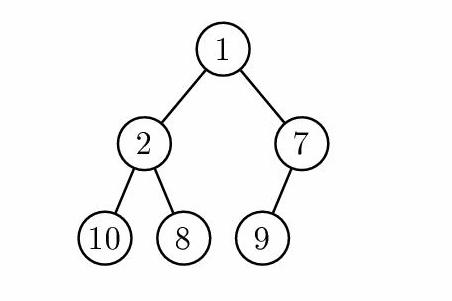
\includegraphics[width=1.0\textwidth,height=6.5in,keepaspectratio]{../images/33.png}
\end{center}
\raggedright{}\myfigurewithoutcaption{33}
\end{minipage}\vspace{0.75cm}


A heap is implemented using an array that is indexed from 1 to N,
where N is the number of elements in the heap.

At any time, the heap must satisfy the heap property\\

\TemplateSpaceIndent{$\text{ }${}$\text{ }${}$\text{ }${}array{$\text{[}$}n{$\text{]}$}$\text{ }${}<{}=$\text{ }${}array{$\text{[}$}2*n{$\text{]}$}$\text{ }${}$\text{ }${}$\text{ }${}//$\text{ }${}parent$\text{ }${}element$\text{ }${}<{}=$\text{ }${}left$\text{ }${}child}

and\\

\TemplateSpaceIndent{$\text{ }${}$\text{ }${}$\text{ }${}array{$\text{[}$}n{$\text{]}$}$\text{ }${}<{}=$\text{ }${}array{$\text{[}$}2*n+1{$\text{]}$}$\text{ }${}//$\text{ }${}parent$\text{ }${}element$\text{ }${}<{}=$\text{ }${}right$\text{ }${}child}

whenever the indices are in the arrays bounds.
\section{Compute the extreme value}
\label{97}
We will prove that {\ttfamily \setmainfont[Path=/usr/share/fonts/truetype/cmu/,UprightFont=cmunrm.ttf,BoldFont=cmunbx.ttf,ItalicFont=cmunti.ttf,BoldItalicFont=cmunbi.ttf]{cmuntt.ttf}\setmonofont[Path=/usr/share/fonts/truetype/cmu/,UprightFont=cmuntt.ttf,BoldFont=cmuntb.ttf,ItalicFont=cmunit.ttf,BoldItalicFont=cmuntx.ttf]{cmuntt.ttf}\ttfamily array{$\text{[}$}1{$\text{]}$}} \setmainfont[Path=/usr/share/fonts/truetype/cmu/,UprightFont=cmunrm.ttf,BoldFont=cmunbx.ttf,ItalicFont=cmunti.ttf,BoldItalicFont=cmunbi.ttf]{cmunrm.ttf}\setmonofont[Path=/usr/share/fonts/truetype/cmu/,UprightFont=cmuntt.ttf,BoldFont=cmuntb.ttf,ItalicFont=cmunit.ttf,BoldItalicFont=cmuntx.ttf]{cmunrm.ttf} is the minimum element in the heap.
We prove it by seeing a contradiction if some other element is less than the first element.
Suppose {\ttfamily \setmainfont[Path=/usr/share/fonts/truetype/cmu/,UprightFont=cmunrm.ttf,BoldFont=cmunbx.ttf,ItalicFont=cmunti.ttf,BoldItalicFont=cmunbi.ttf]{cmuntt.ttf}\setmonofont[Path=/usr/share/fonts/truetype/cmu/,UprightFont=cmuntt.ttf,BoldFont=cmuntb.ttf,ItalicFont=cmunit.ttf,BoldItalicFont=cmuntx.ttf]{cmuntt.ttf}\ttfamily array{$\text{[}$}i{$\text{]}$}} \setmainfont[Path=/usr/share/fonts/truetype/cmu/,UprightFont=cmunrm.ttf,BoldFont=cmunbx.ttf,ItalicFont=cmunti.ttf,BoldItalicFont=cmunbi.ttf]{cmunrm.ttf}\setmonofont[Path=/usr/share/fonts/truetype/cmu/,UprightFont=cmuntt.ttf,BoldFont=cmuntb.ttf,ItalicFont=cmunit.ttf,BoldItalicFont=cmuntx.ttf]{cmunrm.ttf} is the first instance of the minimum,
with {\ttfamily \setmainfont[Path=/usr/share/fonts/truetype/cmu/,UprightFont=cmunrm.ttf,BoldFont=cmunbx.ttf,ItalicFont=cmunti.ttf,BoldItalicFont=cmunbi.ttf]{cmuntt.ttf}\setmonofont[Path=/usr/share/fonts/truetype/cmu/,UprightFont=cmuntt.ttf,BoldFont=cmuntb.ttf,ItalicFont=cmunit.ttf,BoldItalicFont=cmuntx.ttf]{cmuntt.ttf}\ttfamily array{$\text{[}$}j{$\text{]}$} >{} array{$\text{[}$}i{$\text{]}$}} \setmainfont[Path=/usr/share/fonts/truetype/cmu/,UprightFont=cmunrm.ttf,BoldFont=cmunbx.ttf,ItalicFont=cmunti.ttf,BoldItalicFont=cmunbi.ttf]{cmunrm.ttf}\setmonofont[Path=/usr/share/fonts/truetype/cmu/,UprightFont=cmuntt.ttf,BoldFont=cmuntb.ttf,ItalicFont=cmunit.ttf,BoldItalicFont=cmuntx.ttf]{cmunrm.ttf} for all {\ttfamily \setmainfont[Path=/usr/share/fonts/truetype/cmu/,UprightFont=cmunrm.ttf,BoldFont=cmunbx.ttf,ItalicFont=cmunti.ttf,BoldItalicFont=cmunbi.ttf]{cmuntt.ttf}\setmonofont[Path=/usr/share/fonts/truetype/cmu/,UprightFont=cmuntt.ttf,BoldFont=cmuntb.ttf,ItalicFont=cmunit.ttf,BoldItalicFont=cmuntx.ttf]{cmuntt.ttf}\ttfamily j <{} i} \setmainfont[Path=/usr/share/fonts/truetype/cmu/,UprightFont=cmunrm.ttf,BoldFont=cmunbx.ttf,ItalicFont=cmunti.ttf,BoldItalicFont=cmunbi.ttf]{cmunrm.ttf}\setmonofont[Path=/usr/share/fonts/truetype/cmu/,UprightFont=cmuntt.ttf,BoldFont=cmuntb.ttf,ItalicFont=cmunit.ttf,BoldItalicFont=cmuntx.ttf]{cmunrm.ttf}, and {\ttfamily \setmainfont[Path=/usr/share/fonts/truetype/cmu/,UprightFont=cmunrm.ttf,BoldFont=cmunbx.ttf,ItalicFont=cmunti.ttf,BoldItalicFont=cmunbi.ttf]{cmuntt.ttf}\setmonofont[Path=/usr/share/fonts/truetype/cmu/,UprightFont=cmuntt.ttf,BoldFont=cmuntb.ttf,ItalicFont=cmunit.ttf,BoldItalicFont=cmuntx.ttf]{cmuntt.ttf}\ttfamily i >{}= 2} \setmainfont[Path=/usr/share/fonts/truetype/cmu/,UprightFont=cmunrm.ttf,BoldFont=cmunbx.ttf,ItalicFont=cmunti.ttf,BoldItalicFont=cmunbi.ttf]{cmunrm.ttf}\setmonofont[Path=/usr/share/fonts/truetype/cmu/,UprightFont=cmuntt.ttf,BoldFont=cmuntb.ttf,ItalicFont=cmunit.ttf,BoldItalicFont=cmuntx.ttf]{cmunrm.ttf}.
But by the heap invariant array, {\ttfamily \setmainfont[Path=/usr/share/fonts/truetype/cmu/,UprightFont=cmunrm.ttf,BoldFont=cmunbx.ttf,ItalicFont=cmunti.ttf,BoldItalicFont=cmunbi.ttf]{cmuntt.ttf}\setmonofont[Path=/usr/share/fonts/truetype/cmu/,UprightFont=cmuntt.ttf,BoldFont=cmuntb.ttf,ItalicFont=cmunit.ttf,BoldItalicFont=cmuntx.ttf]{cmuntt.ttf}\ttfamily array{$\text{[}$}floor(i/2){$\text{]}$} <{}= array{$\text{[}$}i{$\text{]}$}} \setmainfont[Path=/usr/share/fonts/truetype/cmu/,UprightFont=cmunrm.ttf,BoldFont=cmunbx.ttf,ItalicFont=cmunti.ttf,BoldItalicFont=cmunbi.ttf]{cmunrm.ttf}\setmonofont[Path=/usr/share/fonts/truetype/cmu/,UprightFont=cmuntt.ttf,BoldFont=cmuntb.ttf,ItalicFont=cmunit.ttf,BoldItalicFont=cmuntx.ttf]{cmunrm.ttf}:
this is a contradiction.

Therefore, it is easy to compute {\ttfamily \setmainfont[Path=/usr/share/fonts/truetype/cmu/,UprightFont=cmunrm.ttf,BoldFont=cmunbx.ttf,ItalicFont=cmunti.ttf,BoldItalicFont=cmunbi.ttf]{cmuntt.ttf}\setmonofont[Path=/usr/share/fonts/truetype/cmu/,UprightFont=cmuntt.ttf,BoldFont=cmuntb.ttf,ItalicFont=cmunit.ttf,BoldItalicFont=cmuntx.ttf]{cmuntt.ttf}\ttfamily MIN(heap)} \setmainfont[Path=/usr/share/fonts/truetype/cmu/,UprightFont=cmunrm.ttf,BoldFont=cmunbx.ttf,ItalicFont=cmunti.ttf,BoldItalicFont=cmunbi.ttf]{cmunrm.ttf}\setmonofont[Path=/usr/share/fonts/truetype/cmu/,UprightFont=cmuntt.ttf,BoldFont=cmuntb.ttf,ItalicFont=cmunit.ttf,BoldItalicFont=cmuntx.ttf]{cmunrm.ttf}:\\

\TemplateSpaceIndent{$\text{ }${}$\text{ }${}$\text{ }$\newline{}
$\text{ }${}$\text{ }${}$\text{ }${}MIN(heap)$\text{ }$\newline{}
$\text{ }${}$\text{ }${}$\text{ }${}$\text{ }${}$\text{ }${}$\text{ }${}return$\text{ }${}heap.array{$\text{[}$}1{$\text{]}$};}

\section{Removing the Extreme Value}
\label{98}
To remove the minimum element, we must adjust the heap
to fill {\ttfamily \setmainfont[Path=/usr/share/fonts/truetype/cmu/,UprightFont=cmunrm.ttf,BoldFont=cmunbx.ttf,ItalicFont=cmunti.ttf,BoldItalicFont=cmunbi.ttf]{cmuntt.ttf}\setmonofont[Path=/usr/share/fonts/truetype/cmu/,UprightFont=cmuntt.ttf,BoldFont=cmuntb.ttf,ItalicFont=cmunit.ttf,BoldItalicFont=cmuntx.ttf]{cmuntt.ttf}\ttfamily heap.array{$\text{[}$}1{$\text{]}$}} \setmainfont[Path=/usr/share/fonts/truetype/cmu/,UprightFont=cmunrm.ttf,BoldFont=cmunbx.ttf,ItalicFont=cmunti.ttf,BoldItalicFont=cmunbi.ttf]{cmunrm.ttf}\setmonofont[Path=/usr/share/fonts/truetype/cmu/,UprightFont=cmuntt.ttf,BoldFont=cmuntb.ttf,ItalicFont=cmunit.ttf,BoldItalicFont=cmuntx.ttf]{cmunrm.ttf}.  This process is called {\itshape percolation} \setmainfont[Path=/usr/share/fonts/truetype/cmu/,UprightFont=cmunrm.ttf,BoldFont=cmunbx.ttf,ItalicFont=cmunti.ttf,BoldItalicFont=cmunbi.ttf]{cmunrm.ttf}\setmonofont[Path=/usr/share/fonts/truetype/cmu/,UprightFont=cmuntt.ttf,BoldFont=cmuntb.ttf,ItalicFont=cmunit.ttf,BoldItalicFont=cmuntx.ttf]{cmunrm.ttf}.
Basically, we move the hole from node i to either node {\ttfamily \setmainfont[Path=/usr/share/fonts/truetype/cmu/,UprightFont=cmunrm.ttf,BoldFont=cmunbx.ttf,ItalicFont=cmunti.ttf,BoldItalicFont=cmunbi.ttf]{cmuntt.ttf}\setmonofont[Path=/usr/share/fonts/truetype/cmu/,UprightFont=cmuntt.ttf,BoldFont=cmuntb.ttf,ItalicFont=cmunit.ttf,BoldItalicFont=cmuntx.ttf]{cmuntt.ttf}\ttfamily 2i} \setmainfont[Path=/usr/share/fonts/truetype/cmu/,UprightFont=cmunrm.ttf,BoldFont=cmunbx.ttf,ItalicFont=cmunti.ttf,BoldItalicFont=cmunbi.ttf]{cmunrm.ttf}\setmonofont[Path=/usr/share/fonts/truetype/cmu/,UprightFont=cmuntt.ttf,BoldFont=cmuntb.ttf,ItalicFont=cmunit.ttf,BoldItalicFont=cmuntx.ttf]{cmunrm.ttf} or {\ttfamily \setmainfont[Path=/usr/share/fonts/truetype/cmu/,UprightFont=cmunrm.ttf,BoldFont=cmunbx.ttf,ItalicFont=cmunti.ttf,BoldItalicFont=cmunbi.ttf]{cmuntt.ttf}\setmonofont[Path=/usr/share/fonts/truetype/cmu/,UprightFont=cmuntt.ttf,BoldFont=cmuntb.ttf,ItalicFont=cmunit.ttf,BoldItalicFont=cmuntx.ttf]{cmuntt.ttf}\ttfamily 2i+1} \setmainfont[Path=/usr/share/fonts/truetype/cmu/,UprightFont=cmunrm.ttf,BoldFont=cmunbx.ttf,ItalicFont=cmunti.ttf,BoldItalicFont=cmunbi.ttf]{cmunrm.ttf}\setmonofont[Path=/usr/share/fonts/truetype/cmu/,UprightFont=cmuntt.ttf,BoldFont=cmuntb.ttf,ItalicFont=cmunit.ttf,BoldItalicFont=cmuntx.ttf]{cmunrm.ttf}.
If we pick the minimum of these two, the heap invariant will be maintained;
suppose {\ttfamily \setmainfont[Path=/usr/share/fonts/truetype/cmu/,UprightFont=cmunrm.ttf,BoldFont=cmunbx.ttf,ItalicFont=cmunti.ttf,BoldItalicFont=cmunbi.ttf]{cmuntt.ttf}\setmonofont[Path=/usr/share/fonts/truetype/cmu/,UprightFont=cmuntt.ttf,BoldFont=cmuntb.ttf,ItalicFont=cmunit.ttf,BoldItalicFont=cmuntx.ttf]{cmuntt.ttf}\ttfamily array{$\text{[}$}2i{$\text{]}$} <{} array{$\text{[}$}2i+1{$\text{]}$}} \setmainfont[Path=/usr/share/fonts/truetype/cmu/,UprightFont=cmunrm.ttf,BoldFont=cmunbx.ttf,ItalicFont=cmunti.ttf,BoldItalicFont=cmunbi.ttf]{cmunrm.ttf}\setmonofont[Path=/usr/share/fonts/truetype/cmu/,UprightFont=cmuntt.ttf,BoldFont=cmuntb.ttf,ItalicFont=cmunit.ttf,BoldItalicFont=cmuntx.ttf]{cmunrm.ttf}.  Then {\ttfamily \setmainfont[Path=/usr/share/fonts/truetype/cmu/,UprightFont=cmunrm.ttf,BoldFont=cmunbx.ttf,ItalicFont=cmunti.ttf,BoldItalicFont=cmunbi.ttf]{cmuntt.ttf}\setmonofont[Path=/usr/share/fonts/truetype/cmu/,UprightFont=cmuntt.ttf,BoldFont=cmuntb.ttf,ItalicFont=cmunit.ttf,BoldItalicFont=cmuntx.ttf]{cmuntt.ttf}\ttfamily array{$\text{[}$}2i{$\text{]}$}} \setmainfont[Path=/usr/share/fonts/truetype/cmu/,UprightFont=cmunrm.ttf,BoldFont=cmunbx.ttf,ItalicFont=cmunti.ttf,BoldItalicFont=cmunbi.ttf]{cmunrm.ttf}\setmonofont[Path=/usr/share/fonts/truetype/cmu/,UprightFont=cmuntt.ttf,BoldFont=cmuntb.ttf,ItalicFont=cmunit.ttf,BoldItalicFont=cmuntx.ttf]{cmunrm.ttf} will be moved to {\ttfamily \setmainfont[Path=/usr/share/fonts/truetype/cmu/,UprightFont=cmunrm.ttf,BoldFont=cmunbx.ttf,ItalicFont=cmunti.ttf,BoldItalicFont=cmunbi.ttf]{cmuntt.ttf}\setmonofont[Path=/usr/share/fonts/truetype/cmu/,UprightFont=cmuntt.ttf,BoldFont=cmuntb.ttf,ItalicFont=cmunit.ttf,BoldItalicFont=cmuntx.ttf]{cmuntt.ttf}\ttfamily array{$\text{[}$}i{$\text{]}$}} \setmainfont[Path=/usr/share/fonts/truetype/cmu/,UprightFont=cmunrm.ttf,BoldFont=cmunbx.ttf,ItalicFont=cmunti.ttf,BoldItalicFont=cmunbi.ttf]{cmunrm.ttf}\setmonofont[Path=/usr/share/fonts/truetype/cmu/,UprightFont=cmuntt.ttf,BoldFont=cmuntb.ttf,ItalicFont=cmunit.ttf,BoldItalicFont=cmuntx.ttf]{cmunrm.ttf},
leaving a hole at {\ttfamily \setmainfont[Path=/usr/share/fonts/truetype/cmu/,UprightFont=cmunrm.ttf,BoldFont=cmunbx.ttf,ItalicFont=cmunti.ttf,BoldItalicFont=cmunbi.ttf]{cmuntt.ttf}\setmonofont[Path=/usr/share/fonts/truetype/cmu/,UprightFont=cmuntt.ttf,BoldFont=cmuntb.ttf,ItalicFont=cmunit.ttf,BoldItalicFont=cmuntx.ttf]{cmuntt.ttf}\ttfamily 2i} \setmainfont[Path=/usr/share/fonts/truetype/cmu/,UprightFont=cmunrm.ttf,BoldFont=cmunbx.ttf,ItalicFont=cmunti.ttf,BoldItalicFont=cmunbi.ttf]{cmunrm.ttf}\setmonofont[Path=/usr/share/fonts/truetype/cmu/,UprightFont=cmuntt.ttf,BoldFont=cmuntb.ttf,ItalicFont=cmunit.ttf,BoldItalicFont=cmuntx.ttf]{cmunrm.ttf}, but after the move {\ttfamily \setmainfont[Path=/usr/share/fonts/truetype/cmu/,UprightFont=cmunrm.ttf,BoldFont=cmunbx.ttf,ItalicFont=cmunti.ttf,BoldItalicFont=cmunbi.ttf]{cmuntt.ttf}\setmonofont[Path=/usr/share/fonts/truetype/cmu/,UprightFont=cmuntt.ttf,BoldFont=cmuntb.ttf,ItalicFont=cmunit.ttf,BoldItalicFont=cmuntx.ttf]{cmuntt.ttf}\ttfamily array{$\text{[}$}i{$\text{]}$} <{} array{$\text{[}$}2i+1{$\text{]}$}} \setmainfont[Path=/usr/share/fonts/truetype/cmu/,UprightFont=cmunrm.ttf,BoldFont=cmunbx.ttf,ItalicFont=cmunti.ttf,BoldItalicFont=cmunbi.ttf]{cmunrm.ttf}\setmonofont[Path=/usr/share/fonts/truetype/cmu/,UprightFont=cmuntt.ttf,BoldFont=cmuntb.ttf,ItalicFont=cmunit.ttf,BoldItalicFont=cmuntx.ttf]{cmunrm.ttf}, so the heap invariant is maintained.
In some cases, {\ttfamily \setmainfont[Path=/usr/share/fonts/truetype/cmu/,UprightFont=cmunrm.ttf,BoldFont=cmunbx.ttf,ItalicFont=cmunti.ttf,BoldItalicFont=cmunbi.ttf]{cmuntt.ttf}\setmonofont[Path=/usr/share/fonts/truetype/cmu/,UprightFont=cmuntt.ttf,BoldFont=cmuntb.ttf,ItalicFont=cmunit.ttf,BoldItalicFont=cmuntx.ttf]{cmuntt.ttf}\ttfamily 2i+1} \setmainfont[Path=/usr/share/fonts/truetype/cmu/,UprightFont=cmunrm.ttf,BoldFont=cmunbx.ttf,ItalicFont=cmunti.ttf,BoldItalicFont=cmunbi.ttf]{cmunrm.ttf}\setmonofont[Path=/usr/share/fonts/truetype/cmu/,UprightFont=cmuntt.ttf,BoldFont=cmuntb.ttf,ItalicFont=cmunit.ttf,BoldItalicFont=cmuntx.ttf]{cmunrm.ttf} will exceed the array bounds, and we are forced to percolate {\ttfamily \setmainfont[Path=/usr/share/fonts/truetype/cmu/,UprightFont=cmunrm.ttf,BoldFont=cmunbx.ttf,ItalicFont=cmunti.ttf,BoldItalicFont=cmunbi.ttf]{cmuntt.ttf}\setmonofont[Path=/usr/share/fonts/truetype/cmu/,UprightFont=cmuntt.ttf,BoldFont=cmuntb.ttf,ItalicFont=cmunit.ttf,BoldItalicFont=cmuntx.ttf]{cmuntt.ttf}\ttfamily 2i} \setmainfont[Path=/usr/share/fonts/truetype/cmu/,UprightFont=cmunrm.ttf,BoldFont=cmunbx.ttf,ItalicFont=cmunti.ttf,BoldItalicFont=cmunbi.ttf]{cmunrm.ttf}\setmonofont[Path=/usr/share/fonts/truetype/cmu/,UprightFont=cmuntt.ttf,BoldFont=cmuntb.ttf,ItalicFont=cmunit.ttf,BoldItalicFont=cmuntx.ttf]{cmunrm.ttf}.  In other cases,
{\ttfamily \setmainfont[Path=/usr/share/fonts/truetype/cmu/,UprightFont=cmunrm.ttf,BoldFont=cmunbx.ttf,ItalicFont=cmunti.ttf,BoldItalicFont=cmunbi.ttf]{cmuntt.ttf}\setmonofont[Path=/usr/share/fonts/truetype/cmu/,UprightFont=cmuntt.ttf,BoldFont=cmuntb.ttf,ItalicFont=cmunit.ttf,BoldItalicFont=cmuntx.ttf]{cmuntt.ttf}\ttfamily 2i} \setmainfont[Path=/usr/share/fonts/truetype/cmu/,UprightFont=cmunrm.ttf,BoldFont=cmunbx.ttf,ItalicFont=cmunti.ttf,BoldItalicFont=cmunbi.ttf]{cmunrm.ttf}\setmonofont[Path=/usr/share/fonts/truetype/cmu/,UprightFont=cmuntt.ttf,BoldFont=cmuntb.ttf,ItalicFont=cmunit.ttf,BoldItalicFont=cmuntx.ttf]{cmunrm.ttf} is also outside the bounds: in that case, we are done.


Therefore, here is the remove algorithm:

\\

\TemplateSpaceIndent{$\text{ }${}\#define$\text{ }${}LEFT(i)$\text{ }${}(2*i)}

\\

\TemplateSpaceIndent{$\text{ }${}\#define$\text{ }${}RIGHT(i)$\text{ }${}(2*i$\text{ }${}+$\text{ }${}1)$\text{ }${}$\text{ }${}}

\\

\TemplateSpaceIndent{$\text{ }${}REMOVE\_MIN(heap)$\text{ }$\newline{}
$\text{ }${}\{$\text{ }${}$\text{ }${}$\text{ }$\newline{}
$\text{ }${}$\text{ }${}$\text{ }${}$\text{ }${}$\text{ }${}savemin=arr{$\text{[}$}1{$\text{]}$};$\text{ }$\newline{}
$\text{ }${}$\text{ }${}$\text{ }${}$\text{ }${}$\text{ }${}arr{$\text{[}$}1{$\text{]}$}=arr{$\text{[}$}-{}-{}heapsize{$\text{]}$};$\text{ }$\newline{}
$\text{ }${}$\text{ }${}$\text{ }${}$\text{ }${}$\text{ }${}i=1;$\text{ }$\newline{}
$\text{ }${}$\text{ }${}$\text{ }${}$\text{ }${}$\text{ }${}while(i<{}heapsize)\{$\text{ }$\newline{}
$\text{ }${}$\text{ }${}$\text{ }${}$\text{ }${}$\text{ }${}$\text{ }${}$\text{ }${}$\text{ }${}$\text{ }${}minidx=i;$\text{ }$\newline{}
$\text{ }${}$\text{ }${}$\text{ }${}$\text{ }${}$\text{ }${}$\text{ }${}$\text{ }${}$\text{ }${}$\text{ }${}if(LEFT(i)<{}heapsize$\text{ }${}\&\&$\text{ }${}arr{$\text{[}$}LEFT(i){$\text{]}$}$\text{ }${}<{}$\text{ }${}arr{$\text{[}$}minidx{$\text{]}$})$\text{ }$\newline{}
$\text{ }${}$\text{ }${}$\text{ }${}$\text{ }${}$\text{ }${}$\text{ }${}$\text{ }${}$\text{ }${}$\text{ }${}$\text{ }${}$\text{ }${}$\text{ }${}$\text{ }${}minidx=LEFT(i);$\text{ }$\newline{}
$\text{ }${}$\text{ }${}$\text{ }${}$\text{ }${}$\text{ }${}$\text{ }${}$\text{ }${}$\text{ }${}$\text{ }${}if(RIGHT(i)<{}heapsize$\text{ }${}\&\&$\text{ }${}arr{$\text{[}$}RIGHT(i){$\text{]}$}$\text{ }${}<{}$\text{ }${}arr{$\text{[}$}minidx{$\text{]}$})$\text{ }${}$\text{ }$\newline{}
$\text{ }${}$\text{ }${}$\text{ }${}$\text{ }${}$\text{ }${}$\text{ }${}$\text{ }${}$\text{ }${}$\text{ }${}$\text{ }${}$\text{ }${}$\text{ }${}$\text{ }${}minidx=RIGHT(i);$\text{ }$\newline{}
$\text{ }${}$\text{ }${}$\text{ }${}$\text{ }${}$\text{ }${}$\text{ }${}$\text{ }${}$\text{ }${}$\text{ }${}if(minidx!=i)\{$\text{ }$\newline{}
$\text{ }${}$\text{ }${}$\text{ }${}$\text{ }${}$\text{ }${}$\text{ }${}$\text{ }${}$\text{ }${}$\text{ }${}$\text{ }${}$\text{ }${}$\text{ }${}$\text{ }${}swap(arr{$\text{[}$}i{$\text{]}$},arr{$\text{[}$}minidx{$\text{]}$});$\text{ }$\newline{}
$\text{ }${}$\text{ }${}$\text{ }${}$\text{ }${}$\text{ }${}$\text{ }${}$\text{ }${}$\text{ }${}$\text{ }${}$\text{ }${}$\text{ }${}$\text{ }${}$\text{ }${}i=minidx;$\text{ }${}$\text{ }${}$\text{ }${}$\text{ }${}$\text{ }${}$\text{ }${}$\text{ }${}$\text{ }${}$\text{ }${}$\text{ }${}$\text{ }${}$\text{ }${}$\text{ }$\newline{}
$\text{ }${}$\text{ }${}$\text{ }${}$\text{ }${}$\text{ }${}$\text{ }${}$\text{ }${}$\text{ }${}$\text{ }${}\}$\text{ }$\newline{}
$\text{ }${}$\text{ }${}$\text{ }${}$\text{ }${}$\text{ }${}$\text{ }${}$\text{ }${}$\text{ }${}$\text{ }${}else$\text{ }${}$\text{ }$\newline{}
$\text{ }${}$\text{ }${}$\text{ }${}$\text{ }${}$\text{ }${}$\text{ }${}$\text{ }${}$\text{ }${}$\text{ }${}$\text{ }${}$\text{ }${}$\text{ }${}$\text{ }${}break;$\text{ }$\newline{}
$\text{ }${}$\text{ }${}$\text{ }${}$\text{ }${}$\text{ }${}\}$\text{ }$\newline{}
$\text{ }${}\}}


Why does this work?\\

\TemplateSpaceIndent{$\text{ }${}$\text{ }${}$\text{ }${}$\text{ }${}If$\text{ }${}there$\text{ }${}is$\text{ }${}only$\text{ }${}1$\text{ }${}element$\text{ }${},heapsize$\text{ }${}becomes$\text{ }${}0,$\text{ }${}nothing$\text{ }${}in$\text{ }${}the$\text{ }${}array$\text{ }${}is$\text{ }$\newline{}
$\text{ }${}valid.$\text{ }$\newline{}
$\text{ }${}$\text{ }${}$\text{ }${}$\text{ }${}If$\text{ }${}there$\text{ }${}are$\text{ }${}2$\text{ }${}elements$\text{ }${},$\text{ }${}one$\text{ }${}min$\text{ }${}and$\text{ }${}other$\text{ }${}max,$\text{ }${}you$\text{ }${}replace$\text{ }${}min$\text{ }${}with$\text{ }${}max.$\text{ }$\newline{}
$\text{ }${}$\text{ }${}$\text{ }${}$\text{ }${}If$\text{ }${}there$\text{ }${}are$\text{ }${}3$\text{ }${}or$\text{ }${}more$\text{ }${}elements$\text{ }${}say$\text{ }${}n,$\text{ }${}you$\text{ }${}replace$\text{ }${}0th$\text{ }${}element$\text{ }${}with$\text{ }${}n-{}1th$\text{ }$\newline{}
$\text{ }${}element.$\text{ }${}$\text{ }$\newline{}
$\text{ }${}$\text{ }${}$\text{ }${}$\text{ }${}The$\text{ }${}heap$\text{ }${}property$\text{ }${}is$\text{ }${}destroyed.$\text{ }${}Choose$\text{ }${}the$\text{ }${}2$\text{ }${}children$\text{ }${}of$\text{ }${}root$\text{ }${}and$\text{ }${}check$\text{ }$\newline{}
$\text{ }${}which$\text{ }${}is$\text{ }${}the$\text{ }${}minimum.$\text{ }$\newline{}
$\text{ }${}$\text{ }${}$\text{ }${}$\text{ }${}Choose$\text{ }${}the$\text{ }${}minimum$\text{ }${}between$\text{ }${}them,$\text{ }${}swap$\text{ }${}it.$\text{ }${}Now$\text{ }${}subtree$\text{ }${}with$\text{ }${}swapped$\text{ }${}child$\text{ }${}is$\text{ }$\newline{}
$\text{ }${}loose$\text{ }${}heap$\text{ }${}property.$\text{ }$\newline{}
$\text{ }${}$\text{ }${}$\text{ }${}$\text{ }${}If$\text{ }${}no$\text{ }${}violations$\text{ }${}break.}

\section{Inserting a value into the heap}
\label{99}
A similar strategy exists for INSERT:  just append the element to the array,
then fixup the heap-{}invariants by swapping.
For example if we just appended element N,
then the only invariant violation possible involves that element,
in particular if {$array[floor(N/2)] > array[N]$},
then those two elements must be swapped and
now the only invariant violation possible is between\\

\TemplateSpaceIndent{$\text{ }${}$\text{ }${}array{$\text{[}$}floor(N/4){$\text{]}$}$\text{ }${}$\text{ }${}and$\text{ }${}$\text{ }${}array{$\text{[}$}floor(N/2){$\text{]}$}}

we continue iterating until N=1 or until the invariant is satisfied.\\

\TemplateSpaceIndent{$\text{ }${}$\text{ }$\newline{}
$\text{ }${}INSERT(heap,$\text{ }${}element)$\text{ }$\newline{}
$\text{ }${}$\text{ }${}$\text{ }${}$\text{ }${}append(heap.array,$\text{ }${}element)$\text{ }$\newline{}
$\text{ }${}$\text{ }${}$\text{ }${}$\text{ }${}i$\text{ }${}=$\text{ }${}heap.array.length$\text{ }$\newline{}
$\text{ }${}$\text{ }${}$\text{ }${}$\text{ }${}while$\text{ }${}(i$\text{ }${}>{}$\text{ }${}1)$\text{ }$\newline{}
$\text{ }${}$\text{ }${}$\text{ }${}$\text{ }${}$\text{ }${}$\text{ }${}\{$\text{ }$\newline{}
$\text{ }${}$\text{ }${}$\text{ }${}$\text{ }${}$\text{ }${}$\text{ }${}$\text{ }${}$\text{ }${}if$\text{ }${}(heap.array{$\text{[}$}i/2{$\text{]}$}$\text{ }${}<{}=$\text{ }${}heap.array{$\text{[}$}i{$\text{]}$})$\text{ }$\newline{}
$\text{ }${}$\text{ }${}$\text{ }${}$\text{ }${}$\text{ }${}$\text{ }${}$\text{ }${}$\text{ }${}$\text{ }${}$\text{ }${}break;$\text{ }$\newline{}
$\text{ }${}$\text{ }${}$\text{ }${}$\text{ }${}$\text{ }${}$\text{ }${}$\text{ }${}$\text{ }${}swap(heap.array{$\text{[}$}i/2{$\text{]}$},$\text{ }${}heap.array{$\text{[}$}i{$\text{]}$});$\text{ }$\newline{}
$\text{ }${}$\text{ }${}$\text{ }${}$\text{ }${}$\text{ }${}$\text{ }${}$\text{ }${}$\text{ }${}i$\text{ }${}/=$\text{ }${}2;$\text{ }$\newline{}
$\text{ }${}$\text{ }${}$\text{ }${}$\text{ }${}$\text{ }${}$\text{ }${}\}}

\section{TODO}
\label{100}\\

\TemplateSpaceIndent{$\text{ }${}$\text{ }${}Merge-{}heap:$\text{ }${}it$\text{ }${}would$\text{ }${}take$\text{ }${}two$\text{ }${}max/min$\text{ }${}heap$\text{ }${}and$\text{ }${}merge$\text{ }${}them$\text{ }${}and$\text{ }${}return$\text{ }${}a$\text{ }${}single$\text{ }$\newline{}
$\text{ }${}heap.$\text{ }${}O(n)$\text{ }${}time.$\text{ }$\newline{}
$\text{ }${}$\text{ }${}Make-{}heap:$\text{ }${}it$\text{ }${}would$\text{ }${}also$\text{ }${}be$\text{ }${}nice$\text{ }${}to$\text{ }${}describe$\text{ }${}the$\text{ }${}O(n)$\text{ }${}make-{}heap$\text{ }${}operation$\text{ }$\newline{}
$\text{ }${}$\text{ }${}Heap$\text{ }${}sort:$\text{ }${}the$\text{ }${}structure$\text{ }${}can$\text{ }${}actually$\text{ }${}be$\text{ }${}used$\text{ }${}to$\text{ }${}efficiently$\text{ }${}sort$\text{ }${}arrays$\text{ }$\newline{}
$\text{ }${}$\text{ }${}}


Make-{}heap would make use a function heapify
\\

\TemplateSpaceIndent{$\text{ }${}//Element$\text{ }${}is$\text{ }${}a$\text{ }${}data$\text{ }${}structure//$\text{ }$\newline{}
$\text{ }${}$\text{ }${}$\text{ }${}$\text{ }${}Make-{}heap(Element$\text{ }${}Arr{$\text{[}$}{$\text{]}$},int$\text{ }${}size)$\text{ }${}$\text{ }$\newline{}
$\text{ }${}$\text{ }${}$\text{ }${}$\text{ }${}\{$\text{ }$\newline{}
$\text{ }${}$\text{ }${}$\text{ }${}$\text{ }${}$\text{ }${}$\text{ }${}$\text{ }${}$\text{ }${}for(j=size/2;j>{}0;j-{}-{})$\text{ }$\newline{}
$\text{ }${}$\text{ }${}$\text{ }${}$\text{ }${}$\text{ }${}$\text{ }${}$\text{ }${}$\text{ }${}$\text{ }${}$\text{ }${}$\text{ }${}$\text{ }${}\{$\text{ }$\newline{}
$\text{ }${}$\text{ }${}$\text{ }${}$\text{ }${}$\text{ }${}$\text{ }${}$\text{ }${}$\text{ }${}$\text{ }${}$\text{ }${}$\text{ }${}$\text{ }${}$\text{ }${}$\text{ }${}$\text{ }${}$\text{ }${}Heapify(Arr,size,j);$\text{ }$\newline{}
$\text{ }${}$\text{ }${}$\text{ }${}$\text{ }${}$\text{ }${}$\text{ }${}$\text{ }${}$\text{ }${}$\text{ }${}$\text{ }${}$\text{ }${}$\text{ }${}\}$\text{ }$\newline{}
$\text{ }${}$\text{ }${}$\text{ }${}$\text{ }${}\}}

\\

\TemplateSpaceIndent{$\text{ }${}$\text{ }${}$\text{ }${}$\text{ }${}Heapify(Element$\text{ }${}Arr{$\text{[}$}{$\text{]}$},int$\text{ }${}size,int$\text{ }${}t)$\text{ }$\newline{}
$\text{ }${}$\text{ }${}$\text{ }${}$\text{ }${}\{$\text{ }$\newline{}
$\text{ }${}$\text{ }${}$\text{ }${}$\text{ }${}$\text{ }${}$\text{ }${}$\text{ }${}$\text{ }${}L=2*t;$\text{ }$\newline{}
$\text{ }${}$\text{ }${}$\text{ }${}$\text{ }${}$\text{ }${}$\text{ }${}$\text{ }${}$\text{ }${}R=2*t+1;$\text{ }$\newline{}
$\text{ }${}$\text{ }${}$\text{ }${}$\text{ }${}$\text{ }${}$\text{ }${}$\text{ }${}$\text{ }${}if(L<{}size$\text{ }${})$\text{ }$\newline{}
$\text{ }${}$\text{ }${}$\text{ }${}$\text{ }${}$\text{ }${}$\text{ }${}$\text{ }${}$\text{ }${}\{$\text{ }$\newline{}
$\text{ }${}$\text{ }${}$\text{ }${}$\text{ }${}$\text{ }${}$\text{ }${}$\text{ }${}$\text{ }${}$\text{ }${}$\text{ }${}$\text{ }${}$\text{ }${}mix=minindex(Arr,L,t);$\text{ }$\newline{}
$\text{ }${}$\text{ }${}$\text{ }${}$\text{ }${}$\text{ }${}$\text{ }${}$\text{ }${}$\text{ }${}$\text{ }${}$\text{ }${}$\text{ }${}$\text{ }${}if(R<{}=size)$\text{ }$\newline{}
$\text{ }${}$\text{ }${}$\text{ }${}$\text{ }${}$\text{ }${}$\text{ }${}$\text{ }${}$\text{ }${}$\text{ }${}$\text{ }${}$\text{ }${}$\text{ }${}$\text{ }${}$\text{ }${}$\text{ }${}$\text{ }${}mix=minindex(Arr,R,mix);$\text{ }$\newline{}
$\text{ }${}$\text{ }${}$\text{ }${}$\text{ }${}$\text{ }${}$\text{ }${}$\text{ }${}$\text{ }${}\}$\text{ }$\newline{}
$\text{ }${}$\text{ }${}$\text{ }${}$\text{ }${}$\text{ }${}$\text{ }${}$\text{ }${}$\text{ }${}else$\text{ }$\newline{}
$\text{ }${}$\text{ }${}$\text{ }${}$\text{ }${}$\text{ }${}$\text{ }${}$\text{ }${}$\text{ }${}$\text{ }${}$\text{ }${}$\text{ }${}$\text{ }${}mix=t;$\text{ }$\newline{}
$\text{ }${}$\text{ }${}$\text{ }${}$\text{ }${}$\text{ }${}$\text{ }${}$\text{ }${}$\text{ }${}if(mix!=t)$\text{ }$\newline{}
$\text{ }${}$\text{ }${}$\text{ }${}$\text{ }${}$\text{ }${}$\text{ }${}$\text{ }${}$\text{ }${}\{$\text{ }$\newline{}
$\text{ }${}$\text{ }${}$\text{ }${}$\text{ }${}$\text{ }${}$\text{ }${}$\text{ }${}$\text{ }${}$\text{ }${}$\text{ }${}$\text{ }${}$\text{ }${}swap(mix,t);$\text{ }$\newline{}
$\text{ }${}$\text{ }${}$\text{ }${}$\text{ }${}$\text{ }${}$\text{ }${}$\text{ }${}$\text{ }${}$\text{ }${}$\text{ }${}$\text{ }${}$\text{ }${}Heapify(Arr,size,mix);$\text{ }$\newline{}
$\text{ }${}$\text{ }${}$\text{ }${}$\text{ }${}$\text{ }${}$\text{ }${}$\text{ }${}$\text{ }${}\}$\text{ }$\newline{}
$\text{ }${}$\text{ }${}$\text{ }${}$\text{ }${}\}}


minindex returns index of the smaller element
\section{Applications of Priority Heaps}
\label{101}
In 2009, a smaller Sort Benchmark was won by OzSort, which has a paper describing lucidly how to use a priority heap
as the sorting machine to produce merged parts of large (internally) sorted sections . If a sorted section took M memory
and the sorting problem was k x M big, then take  sequential sections of each of the k sections of size M/k , at a time, so they
fit in M memory ( k * M/k = M ), and feed the first element of each of k sections to make a k sized priority queue, and as the top element
is removed and written to an output buffer, take the next element from the corresponding section. This means elements may need
to be associated with a label for the section they come from. When a M/k-{}sized section is exhausted, load in the next
M/k sized minisection from the original sorted section stored on disc. Continue until all minisections in each of the
k sections on disc have been exhausted. 

(As an example of pipelining to fill up disc operational delays, there are twin output buffers, so that once an output buffer is full
one gets written the disc while the other is being filled.)

This paper showed that a priority heap is more straightforward than
a binary tree, because elements are constantly being deleted, as well as added, as a queuing mechanism for a k way merge, and has
practical application for sorting large sets of data that exceed internal memory storage.


\LaTeXNullTemplate{}

\label{102}
\LaTeXNullTemplate{}
\section{Graphs}
\label{103}
A {\bfseries \setmainfont[Path=/usr/share/fonts/truetype/cmu/,UprightFont=cmunrm.ttf,BoldFont=cmunbx.ttf,ItalicFont=cmunti.ttf,BoldItalicFont=cmunbi.ttf]{cmunbx.ttf}\setmonofont[Path=/usr/share/fonts/truetype/cmu/,UprightFont=cmuntt.ttf,BoldFont=cmuntb.ttf,ItalicFont=cmunit.ttf,BoldItalicFont=cmuntx.ttf]{cmunbx.ttf}\bfseries graph} \setmainfont[Path=/usr/share/fonts/truetype/cmu/,UprightFont=cmunrm.ttf,BoldFont=cmunbx.ttf,ItalicFont=cmunti.ttf,BoldItalicFont=cmunbi.ttf]{cmunrm.ttf}\setmonofont[Path=/usr/share/fonts/truetype/cmu/,UprightFont=cmuntt.ttf,BoldFont=cmuntb.ttf,ItalicFont=cmunit.ttf,BoldItalicFont=cmuntx.ttf]{cmunrm.ttf} is a structure consisting of a set of arrays (also called dimensions) {$\{v_1, v_2,\dots,v_n\}$} and a set of edges  {$\{e_1, e_2,\dots,e_m\}$}.  An edge is a pair of vertices {$\{v_i, v_j\}\ i,j \in \{1..n\}$}.  The two vertices are called the edge {\itshape endpoints} \setmainfont[Path=/usr/share/fonts/truetype/cmu/,UprightFont=cmunrm.ttf,BoldFont=cmunbx.ttf,ItalicFont=cmunti.ttf,BoldItalicFont=cmunbi.ttf]{cmunrm.ttf}\setmonofont[Path=/usr/share/fonts/truetype/cmu/,UprightFont=cmuntt.ttf,BoldFont=cmuntb.ttf,ItalicFont=cmunit.ttf,BoldItalicFont=cmuntx.ttf]{cmunrm.ttf}.  Graphs are ubiquitous in computer science.  They are used to model real-{}world systems such as the Internet (each node represents a router and each edge represents a connection between routers); airline connections (each node is an airport and each edge is a flight); or a city road network (each node represents an intersection and each edge represents a block).  The wireframe drawings in computer graphics are another example of graphs.  

A graph may be either {\itshape undirected} \setmainfont[Path=/usr/share/fonts/truetype/cmu/,UprightFont=cmunrm.ttf,BoldFont=cmunbx.ttf,ItalicFont=cmunti.ttf,BoldItalicFont=cmunbi.ttf]{cmunrm.ttf}\setmonofont[Path=/usr/share/fonts/truetype/cmu/,UprightFont=cmuntt.ttf,BoldFont=cmuntb.ttf,ItalicFont=cmunit.ttf,BoldItalicFont=cmuntx.ttf]{cmunrm.ttf} or {\itshape directed} \setmainfont[Path=/usr/share/fonts/truetype/cmu/,UprightFont=cmunrm.ttf,BoldFont=cmunbx.ttf,ItalicFont=cmunti.ttf,BoldItalicFont=cmunbi.ttf]{cmunrm.ttf}\setmonofont[Path=/usr/share/fonts/truetype/cmu/,UprightFont=cmuntt.ttf,BoldFont=cmuntb.ttf,ItalicFont=cmunit.ttf,BoldItalicFont=cmuntx.ttf]{cmunrm.ttf}.  Intuitively, an undirected edge models a \symbol{34}two-{}way\symbol{34} or \symbol{34}duplex\symbol{34} connection between its endpoints, while a directed edge is a one-{}way connection, and is typically drawn as an arrow.  A directed edge is often called an {\itshape arc} \setmainfont[Path=/usr/share/fonts/truetype/cmu/,UprightFont=cmunrm.ttf,BoldFont=cmunbx.ttf,ItalicFont=cmunti.ttf,BoldItalicFont=cmunbi.ttf]{cmunrm.ttf}\setmonofont[Path=/usr/share/fonts/truetype/cmu/,UprightFont=cmuntt.ttf,BoldFont=cmuntb.ttf,ItalicFont=cmunit.ttf,BoldItalicFont=cmuntx.ttf]{cmunrm.ttf}.  Mathematically, an undirected edge is an unordered pair of vertices, and an arc is an ordered pair.  For example, a road network might be modeled as a directed graph, with one-{}way streets indicated by an arrow between endpoints in the appropriate direction, and two-{}way streets shown by a pair of parallel directed edges going both directions between the endpoints.  You might ask, why not use a single {\itshape undirected} \setmainfont[Path=/usr/share/fonts/truetype/cmu/,UprightFont=cmunrm.ttf,BoldFont=cmunbx.ttf,ItalicFont=cmunti.ttf,BoldItalicFont=cmunbi.ttf]{cmunrm.ttf}\setmonofont[Path=/usr/share/fonts/truetype/cmu/,UprightFont=cmuntt.ttf,BoldFont=cmuntb.ttf,ItalicFont=cmunit.ttf,BoldItalicFont=cmuntx.ttf]{cmunrm.ttf} edge for a two-{}way street.  There\textquotesingle{}s no theoretical problem with this, but from a practical programming standpoint, it\textquotesingle{}s generally simpler and less error-{}prone to stick with all directed or all undirected edges.

An undirected graph can have at most {$\left (    \begin{array}{c}    n+1 \\ 2        \end{array}    \right )$} edges (one for each unordered pair), while a directed graph can have at most {$n^2$} edges (one per ordered pair).  A graph is called {\itshape sparse} \setmainfont[Path=/usr/share/fonts/truetype/cmu/,UprightFont=cmunrm.ttf,BoldFont=cmunbx.ttf,ItalicFont=cmunti.ttf,BoldItalicFont=cmunbi.ttf]{cmunrm.ttf}\setmonofont[Path=/usr/share/fonts/truetype/cmu/,UprightFont=cmuntt.ttf,BoldFont=cmuntb.ttf,ItalicFont=cmunit.ttf,BoldItalicFont=cmuntx.ttf]{cmunrm.ttf} if it has many fewer than this many edges (typically {$O(n)$} edges), and {\itshape dense} \setmainfont[Path=/usr/share/fonts/truetype/cmu/,UprightFont=cmunrm.ttf,BoldFont=cmunbx.ttf,ItalicFont=cmunti.ttf,BoldItalicFont=cmunbi.ttf]{cmunrm.ttf}\setmonofont[Path=/usr/share/fonts/truetype/cmu/,UprightFont=cmuntt.ttf,BoldFont=cmuntb.ttf,ItalicFont=cmunit.ttf,BoldItalicFont=cmuntx.ttf]{cmunrm.ttf} if it has closer to {$\Omega(n^2)$} edges.  A {\bfseries \setmainfont[Path=/usr/share/fonts/truetype/cmu/,UprightFont=cmunrm.ttf,BoldFont=cmunbx.ttf,ItalicFont=cmunti.ttf,BoldItalicFont=cmunbi.ttf]{cmunbx.ttf}\setmonofont[Path=/usr/share/fonts/truetype/cmu/,UprightFont=cmuntt.ttf,BoldFont=cmuntb.ttf,ItalicFont=cmunit.ttf,BoldItalicFont=cmuntx.ttf]{cmunbx.ttf}\bfseries multigraph} \setmainfont[Path=/usr/share/fonts/truetype/cmu/,UprightFont=cmunrm.ttf,BoldFont=cmunbx.ttf,ItalicFont=cmunti.ttf,BoldItalicFont=cmunbi.ttf]{cmunrm.ttf}\setmonofont[Path=/usr/share/fonts/truetype/cmu/,UprightFont=cmuntt.ttf,BoldFont=cmuntb.ttf,ItalicFont=cmunit.ttf,BoldItalicFont=cmuntx.ttf]{cmunrm.ttf} can have more than one edge between the same two vertices.  For example, if one were modeling airline flights, there might be multiple flights between two cities, occurring at different times of the day.

A {\bfseries \setmainfont[Path=/usr/share/fonts/truetype/cmu/,UprightFont=cmunrm.ttf,BoldFont=cmunbx.ttf,ItalicFont=cmunti.ttf,BoldItalicFont=cmunbi.ttf]{cmunbx.ttf}\setmonofont[Path=/usr/share/fonts/truetype/cmu/,UprightFont=cmuntt.ttf,BoldFont=cmuntb.ttf,ItalicFont=cmunit.ttf,BoldItalicFont=cmuntx.ttf]{cmunbx.ttf}\bfseries path} \setmainfont[Path=/usr/share/fonts/truetype/cmu/,UprightFont=cmunrm.ttf,BoldFont=cmunbx.ttf,ItalicFont=cmunti.ttf,BoldItalicFont=cmunbi.ttf]{cmunrm.ttf}\setmonofont[Path=/usr/share/fonts/truetype/cmu/,UprightFont=cmuntt.ttf,BoldFont=cmuntb.ttf,ItalicFont=cmunit.ttf,BoldItalicFont=cmuntx.ttf]{cmunrm.ttf} in a graph is a sequence of vertices {$\{ v_{i_1}, v_{i_2}, \dots , v_{i_k} \}$} such that there exists an edge or arc between consecutive vertices.  The path is called a {\bfseries \setmainfont[Path=/usr/share/fonts/truetype/cmu/,UprightFont=cmunrm.ttf,BoldFont=cmunbx.ttf,ItalicFont=cmunti.ttf,BoldItalicFont=cmunbi.ttf]{cmunbx.ttf}\setmonofont[Path=/usr/share/fonts/truetype/cmu/,UprightFont=cmuntt.ttf,BoldFont=cmuntb.ttf,ItalicFont=cmunit.ttf,BoldItalicFont=cmuntx.ttf]{cmunbx.ttf}\bfseries cycle} \setmainfont[Path=/usr/share/fonts/truetype/cmu/,UprightFont=cmunrm.ttf,BoldFont=cmunbx.ttf,ItalicFont=cmunti.ttf,BoldItalicFont=cmunbi.ttf]{cmunrm.ttf}\setmonofont[Path=/usr/share/fonts/truetype/cmu/,UprightFont=cmuntt.ttf,BoldFont=cmuntb.ttf,ItalicFont=cmunit.ttf,BoldItalicFont=cmuntx.ttf]{cmunrm.ttf} if {$v_{i_1} \equiv v_{i_k}$}.  An undirected acyclic graph is equivalent to an undirected tree.  A directed acyclic graph is called a {\bfseries \setmainfont[Path=/usr/share/fonts/truetype/cmu/,UprightFont=cmunrm.ttf,BoldFont=cmunbx.ttf,ItalicFont=cmunti.ttf,BoldItalicFont=cmunbi.ttf]{cmunbx.ttf}\setmonofont[Path=/usr/share/fonts/truetype/cmu/,UprightFont=cmuntt.ttf,BoldFont=cmuntb.ttf,ItalicFont=cmunit.ttf,BoldItalicFont=cmuntx.ttf]{cmunbx.ttf}\bfseries DAG} \setmainfont[Path=/usr/share/fonts/truetype/cmu/,UprightFont=cmunrm.ttf,BoldFont=cmunbx.ttf,ItalicFont=cmunti.ttf,BoldItalicFont=cmunbi.ttf]{cmunrm.ttf}\setmonofont[Path=/usr/share/fonts/truetype/cmu/,UprightFont=cmuntt.ttf,BoldFont=cmuntb.ttf,ItalicFont=cmunit.ttf,BoldItalicFont=cmuntx.ttf]{cmunrm.ttf}.  It is not necessarily a tree.

Nodes and edges often have associated information, such as {\itshape labels} \setmainfont[Path=/usr/share/fonts/truetype/cmu/,UprightFont=cmunrm.ttf,BoldFont=cmunbx.ttf,ItalicFont=cmunti.ttf,BoldItalicFont=cmunbi.ttf]{cmunrm.ttf}\setmonofont[Path=/usr/share/fonts/truetype/cmu/,UprightFont=cmuntt.ttf,BoldFont=cmuntb.ttf,ItalicFont=cmunit.ttf,BoldItalicFont=cmuntx.ttf]{cmunrm.ttf} or {\itshape weights} \setmainfont[Path=/usr/share/fonts/truetype/cmu/,UprightFont=cmunrm.ttf,BoldFont=cmunbx.ttf,ItalicFont=cmunti.ttf,BoldItalicFont=cmunbi.ttf]{cmunrm.ttf}\setmonofont[Path=/usr/share/fonts/truetype/cmu/,UprightFont=cmuntt.ttf,BoldFont=cmuntb.ttf,ItalicFont=cmunit.ttf,BoldItalicFont=cmuntx.ttf]{cmunrm.ttf}.  For example, in a graph of airline flights, a node might be labeled with the name of the corresponding airport, and an edge might have a weight equal to the flight time.  The popular game \symbol{34}\myhref{http://en.wikipedia.org/wiki/Six_Degrees_of_Kevin_Bacon}{Six Degrees of Kevin Bacon}\symbol{34} can be modeled by a labeled undirected graph. Each actor becomes a node, labeled by the actor\textquotesingle{}s name. Nodes are connected by an edge when the two actors appeared together in some movie. We can label this edge by the name of the movie.  Deciding if an actor is separated from Kevin Bacon by six or fewer steps is equivalent to finding a path of length at most six in the graph between Bacon\textquotesingle{}s vertex and the other actors vertex.  (This can be done with the breadth-{}first search algorithm found in the companion \myhref{http://en.wikibooks.org/wiki/Computer_Science\%3AAlgorithms}{Algorithms} book. The Oracle of Bacon at the University of Virginia has actually implemented this algorithm and can tell you the path from any actor to Kevin Bacon in a few clicks\myplainurl{http://www.cs.virginia.edu/oracle/}.)
\subsection{Directed Graphs}
\label{104}


\begin{minipage}{0.31250\textwidth}
\begin{center}
\includegraphics[width=1.0\textwidth,height=6.5in,keepaspectratio]{../images/34.\SVGExtension}
\end{center}
\raggedright{}\myfigurewithcaption{34}{A directed graph.}
\end{minipage}\vspace{0.75cm}


The number of edges with one endpoint on a given vertex is called that vertex\textquotesingle{}s {\bfseries \setmainfont[Path=/usr/share/fonts/truetype/cmu/,UprightFont=cmunrm.ttf,BoldFont=cmunbx.ttf,ItalicFont=cmunti.ttf,BoldItalicFont=cmunbi.ttf]{cmunbx.ttf}\setmonofont[Path=/usr/share/fonts/truetype/cmu/,UprightFont=cmuntt.ttf,BoldFont=cmuntb.ttf,ItalicFont=cmunit.ttf,BoldItalicFont=cmuntx.ttf]{cmunbx.ttf}\bfseries degree} \setmainfont[Path=/usr/share/fonts/truetype/cmu/,UprightFont=cmunrm.ttf,BoldFont=cmunbx.ttf,ItalicFont=cmunti.ttf,BoldItalicFont=cmunbi.ttf]{cmunrm.ttf}\setmonofont[Path=/usr/share/fonts/truetype/cmu/,UprightFont=cmuntt.ttf,BoldFont=cmuntb.ttf,ItalicFont=cmunit.ttf,BoldItalicFont=cmuntx.ttf]{cmunrm.ttf}. In a directed graph, the number of edges that point {\itshape to} \setmainfont[Path=/usr/share/fonts/truetype/cmu/,UprightFont=cmunrm.ttf,BoldFont=cmunbx.ttf,ItalicFont=cmunti.ttf,BoldItalicFont=cmunbi.ttf]{cmunrm.ttf}\setmonofont[Path=/usr/share/fonts/truetype/cmu/,UprightFont=cmuntt.ttf,BoldFont=cmuntb.ttf,ItalicFont=cmunit.ttf,BoldItalicFont=cmuntx.ttf]{cmunrm.ttf} a given vertex is called its {\bfseries \setmainfont[Path=/usr/share/fonts/truetype/cmu/,UprightFont=cmunrm.ttf,BoldFont=cmunbx.ttf,ItalicFont=cmunti.ttf,BoldItalicFont=cmunbi.ttf]{cmunbx.ttf}\setmonofont[Path=/usr/share/fonts/truetype/cmu/,UprightFont=cmuntt.ttf,BoldFont=cmuntb.ttf,ItalicFont=cmunit.ttf,BoldItalicFont=cmuntx.ttf]{cmunbx.ttf}\bfseries in-{}degree} \setmainfont[Path=/usr/share/fonts/truetype/cmu/,UprightFont=cmunrm.ttf,BoldFont=cmunbx.ttf,ItalicFont=cmunti.ttf,BoldItalicFont=cmunbi.ttf]{cmunrm.ttf}\setmonofont[Path=/usr/share/fonts/truetype/cmu/,UprightFont=cmuntt.ttf,BoldFont=cmuntb.ttf,ItalicFont=cmunit.ttf,BoldItalicFont=cmuntx.ttf]{cmunrm.ttf}, and the number that point {\itshape from} \setmainfont[Path=/usr/share/fonts/truetype/cmu/,UprightFont=cmunrm.ttf,BoldFont=cmunbx.ttf,ItalicFont=cmunti.ttf,BoldItalicFont=cmunbi.ttf]{cmunrm.ttf}\setmonofont[Path=/usr/share/fonts/truetype/cmu/,UprightFont=cmuntt.ttf,BoldFont=cmuntb.ttf,ItalicFont=cmunit.ttf,BoldItalicFont=cmuntx.ttf]{cmunrm.ttf} it is called its {\bfseries \setmainfont[Path=/usr/share/fonts/truetype/cmu/,UprightFont=cmunrm.ttf,BoldFont=cmunbx.ttf,ItalicFont=cmunti.ttf,BoldItalicFont=cmunbi.ttf]{cmunbx.ttf}\setmonofont[Path=/usr/share/fonts/truetype/cmu/,UprightFont=cmuntt.ttf,BoldFont=cmuntb.ttf,ItalicFont=cmunit.ttf,BoldItalicFont=cmuntx.ttf]{cmunbx.ttf}\bfseries out-{}degree} \setmainfont[Path=/usr/share/fonts/truetype/cmu/,UprightFont=cmunrm.ttf,BoldFont=cmunbx.ttf,ItalicFont=cmunti.ttf,BoldItalicFont=cmunbi.ttf]{cmunrm.ttf}\setmonofont[Path=/usr/share/fonts/truetype/cmu/,UprightFont=cmuntt.ttf,BoldFont=cmuntb.ttf,ItalicFont=cmunit.ttf,BoldItalicFont=cmuntx.ttf]{cmunrm.ttf}.  Often, we may want to be able to distinguish between different nodes and edges. We can associate labels with either. We call such a graph {\bfseries \setmainfont[Path=/usr/share/fonts/truetype/cmu/,UprightFont=cmunrm.ttf,BoldFont=cmunbx.ttf,ItalicFont=cmunti.ttf,BoldItalicFont=cmunbi.ttf]{cmunbx.ttf}\setmonofont[Path=/usr/share/fonts/truetype/cmu/,UprightFont=cmuntt.ttf,BoldFont=cmuntb.ttf,ItalicFont=cmunit.ttf,BoldItalicFont=cmuntx.ttf]{cmunbx.ttf}\bfseries labeled} \setmainfont[Path=/usr/share/fonts/truetype/cmu/,UprightFont=cmunrm.ttf,BoldFont=cmunbx.ttf,ItalicFont=cmunti.ttf,BoldItalicFont=cmunbi.ttf]{cmunrm.ttf}\setmonofont[Path=/usr/share/fonts/truetype/cmu/,UprightFont=cmuntt.ttf,BoldFont=cmuntb.ttf,ItalicFont=cmunit.ttf,BoldItalicFont=cmuntx.ttf]{cmunrm.ttf}.

\LaTeXShadedColorBoxTemplate{\definecolor{shadecolor}{rgb}{1.00000,1.00000,0.93333}}{
{\bfseries \setmainfont[Path=/usr/share/fonts/truetype/cmu/,UprightFont=cmunrm.ttf,BoldFont=cmunbx.ttf,ItalicFont=cmunti.ttf,BoldItalicFont=cmunbi.ttf]{cmunbx.ttf}\setmonofont[Path=/usr/share/fonts/truetype/cmu/,UprightFont=cmuntt.ttf,BoldFont=cmuntb.ttf,ItalicFont=cmunit.ttf,BoldItalicFont=cmuntx.ttf]{cmunbx.ttf}\bfseries Directed Graph Operations} \setmainfont[Path=/usr/share/fonts/truetype/cmu/,UprightFont=cmunrm.ttf,BoldFont=cmunbx.ttf,ItalicFont=cmunti.ttf,BoldItalicFont=cmunbi.ttf]{cmunrm.ttf}\setmonofont[Path=/usr/share/fonts/truetype/cmu/,UprightFont=cmuntt.ttf,BoldFont=cmuntb.ttf,ItalicFont=cmunit.ttf,BoldItalicFont=cmuntx.ttf]{cmunrm.ttf}

{\bfseries {\ttfamily {\bfseries \setmainfont[Path=/usr/share/fonts/truetype/cmu/,UprightFont=cmunrm.ttf,BoldFont=cmunbx.ttf,ItalicFont=cmunti.ttf,BoldItalicFont=cmunbi.ttf]{cmuntb.ttf}\setmonofont[Path=/usr/share/fonts/truetype/cmu/,UprightFont=cmuntt.ttf,BoldFont=cmuntb.ttf,ItalicFont=cmunit.ttf,BoldItalicFont=cmuntx.ttf]{cmuntb.ttf}\ttfamily \bfseries make-{}graph} (): graph}} \setmainfont[Path=/usr/share/fonts/truetype/cmu/,UprightFont=cmunrm.ttf,BoldFont=cmunbx.ttf,ItalicFont=cmunti.ttf,BoldItalicFont=cmunbi.ttf]{cmunrm.ttf}\setmonofont[Path=/usr/share/fonts/truetype/cmu/,UprightFont=cmuntt.ttf,BoldFont=cmuntb.ttf,ItalicFont=cmunit.ttf,BoldItalicFont=cmuntx.ttf]{cmunrm.ttf}

\begin{myquote}
\item{}Create a new graph, initially with no nodes or edges.
\end{myquote}


{\bfseries {\ttfamily {\bfseries \setmainfont[Path=/usr/share/fonts/truetype/cmu/,UprightFont=cmunrm.ttf,BoldFont=cmunbx.ttf,ItalicFont=cmunti.ttf,BoldItalicFont=cmunbi.ttf]{cmuntb.ttf}\setmonofont[Path=/usr/share/fonts/truetype/cmu/,UprightFont=cmuntt.ttf,BoldFont=cmuntb.ttf,ItalicFont=cmunit.ttf,BoldItalicFont=cmuntx.ttf]{cmuntb.ttf}\ttfamily \bfseries make-{}vertex} (graph {\ttfamily \bfseries \itshape G} \setmainfont[Path=/usr/share/fonts/truetype/cmu/,UprightFont=cmunrm.ttf,BoldFont=cmunbx.ttf,ItalicFont=cmunti.ttf,BoldItalicFont=cmunbi.ttf]{cmuntb.ttf}\setmonofont[Path=/usr/share/fonts/truetype/cmu/,UprightFont=cmuntt.ttf,BoldFont=cmuntb.ttf,ItalicFont=cmunit.ttf,BoldItalicFont=cmuntx.ttf]{cmuntb.ttf}\ttfamily \bfseries , element {\ttfamily \bfseries \itshape value} \setmainfont[Path=/usr/share/fonts/truetype/cmu/,UprightFont=cmunrm.ttf,BoldFont=cmunbx.ttf,ItalicFont=cmunti.ttf,BoldItalicFont=cmunbi.ttf]{cmuntb.ttf}\setmonofont[Path=/usr/share/fonts/truetype/cmu/,UprightFont=cmuntt.ttf,BoldFont=cmuntb.ttf,ItalicFont=cmunit.ttf,BoldItalicFont=cmuntx.ttf]{cmuntb.ttf}\ttfamily \bfseries ): vertex}} \setmainfont[Path=/usr/share/fonts/truetype/cmu/,UprightFont=cmunrm.ttf,BoldFont=cmunbx.ttf,ItalicFont=cmunti.ttf,BoldItalicFont=cmunbi.ttf]{cmunrm.ttf}\setmonofont[Path=/usr/share/fonts/truetype/cmu/,UprightFont=cmuntt.ttf,BoldFont=cmuntb.ttf,ItalicFont=cmunit.ttf,BoldItalicFont=cmuntx.ttf]{cmunrm.ttf}

\begin{myquote}
\item{}Create a new vertex, with the given value.
\end{myquote}


{\bfseries {\ttfamily {\bfseries \setmainfont[Path=/usr/share/fonts/truetype/cmu/,UprightFont=cmunrm.ttf,BoldFont=cmunbx.ttf,ItalicFont=cmunti.ttf,BoldItalicFont=cmunbi.ttf]{cmuntb.ttf}\setmonofont[Path=/usr/share/fonts/truetype/cmu/,UprightFont=cmuntt.ttf,BoldFont=cmuntb.ttf,ItalicFont=cmunit.ttf,BoldItalicFont=cmuntx.ttf]{cmuntb.ttf}\ttfamily \bfseries make-{}edge} (vertex {\ttfamily \bfseries \itshape u} \setmainfont[Path=/usr/share/fonts/truetype/cmu/,UprightFont=cmunrm.ttf,BoldFont=cmunbx.ttf,ItalicFont=cmunti.ttf,BoldItalicFont=cmunbi.ttf]{cmuntb.ttf}\setmonofont[Path=/usr/share/fonts/truetype/cmu/,UprightFont=cmuntt.ttf,BoldFont=cmuntb.ttf,ItalicFont=cmunit.ttf,BoldItalicFont=cmuntx.ttf]{cmuntb.ttf}\ttfamily \bfseries , vertex {\ttfamily \bfseries \itshape v} \setmainfont[Path=/usr/share/fonts/truetype/cmu/,UprightFont=cmunrm.ttf,BoldFont=cmunbx.ttf,ItalicFont=cmunti.ttf,BoldItalicFont=cmunbi.ttf]{cmuntb.ttf}\setmonofont[Path=/usr/share/fonts/truetype/cmu/,UprightFont=cmuntt.ttf,BoldFont=cmuntb.ttf,ItalicFont=cmunit.ttf,BoldItalicFont=cmuntx.ttf]{cmuntb.ttf}\ttfamily \bfseries ): edge}} \setmainfont[Path=/usr/share/fonts/truetype/cmu/,UprightFont=cmunrm.ttf,BoldFont=cmunbx.ttf,ItalicFont=cmunti.ttf,BoldItalicFont=cmunbi.ttf]{cmunrm.ttf}\setmonofont[Path=/usr/share/fonts/truetype/cmu/,UprightFont=cmuntt.ttf,BoldFont=cmuntb.ttf,ItalicFont=cmunit.ttf,BoldItalicFont=cmuntx.ttf]{cmunrm.ttf}

\begin{myquote}
\item{}Create an edge between {\itshape u} \setmainfont[Path=/usr/share/fonts/truetype/cmu/,UprightFont=cmunrm.ttf,BoldFont=cmunbx.ttf,ItalicFont=cmunti.ttf,BoldItalicFont=cmunbi.ttf]{cmunrm.ttf}\setmonofont[Path=/usr/share/fonts/truetype/cmu/,UprightFont=cmuntt.ttf,BoldFont=cmuntb.ttf,ItalicFont=cmunit.ttf,BoldItalicFont=cmuntx.ttf]{cmunrm.ttf} and {\itshape v} \setmainfont[Path=/usr/share/fonts/truetype/cmu/,UprightFont=cmunrm.ttf,BoldFont=cmunbx.ttf,ItalicFont=cmunti.ttf,BoldItalicFont=cmunbi.ttf]{cmunrm.ttf}\setmonofont[Path=/usr/share/fonts/truetype/cmu/,UprightFont=cmuntt.ttf,BoldFont=cmuntb.ttf,ItalicFont=cmunit.ttf,BoldItalicFont=cmuntx.ttf]{cmunrm.ttf}. In a directed graph, the edge will flow from {\itshape u} \setmainfont[Path=/usr/share/fonts/truetype/cmu/,UprightFont=cmunrm.ttf,BoldFont=cmunbx.ttf,ItalicFont=cmunti.ttf,BoldItalicFont=cmunbi.ttf]{cmunrm.ttf}\setmonofont[Path=/usr/share/fonts/truetype/cmu/,UprightFont=cmuntt.ttf,BoldFont=cmuntb.ttf,ItalicFont=cmunit.ttf,BoldItalicFont=cmuntx.ttf]{cmunrm.ttf} to {\itshape v} \setmainfont[Path=/usr/share/fonts/truetype/cmu/,UprightFont=cmunrm.ttf,BoldFont=cmunbx.ttf,ItalicFont=cmunti.ttf,BoldItalicFont=cmunbi.ttf]{cmunrm.ttf}\setmonofont[Path=/usr/share/fonts/truetype/cmu/,UprightFont=cmuntt.ttf,BoldFont=cmuntb.ttf,ItalicFont=cmunit.ttf,BoldItalicFont=cmuntx.ttf]{cmunrm.ttf}.
\end{myquote}


{\bfseries {\ttfamily {\bfseries \setmainfont[Path=/usr/share/fonts/truetype/cmu/,UprightFont=cmunrm.ttf,BoldFont=cmunbx.ttf,ItalicFont=cmunti.ttf,BoldItalicFont=cmunbi.ttf]{cmuntb.ttf}\setmonofont[Path=/usr/share/fonts/truetype/cmu/,UprightFont=cmuntt.ttf,BoldFont=cmuntb.ttf,ItalicFont=cmunit.ttf,BoldItalicFont=cmuntx.ttf]{cmuntb.ttf}\ttfamily \bfseries get-{}edges} (vertex {\ttfamily \bfseries \itshape v} \setmainfont[Path=/usr/share/fonts/truetype/cmu/,UprightFont=cmunrm.ttf,BoldFont=cmunbx.ttf,ItalicFont=cmunti.ttf,BoldItalicFont=cmunbi.ttf]{cmuntb.ttf}\setmonofont[Path=/usr/share/fonts/truetype/cmu/,UprightFont=cmuntt.ttf,BoldFont=cmuntb.ttf,ItalicFont=cmunit.ttf,BoldItalicFont=cmuntx.ttf]{cmuntb.ttf}\ttfamily \bfseries ): edge-{}set}} \setmainfont[Path=/usr/share/fonts/truetype/cmu/,UprightFont=cmunrm.ttf,BoldFont=cmunbx.ttf,ItalicFont=cmunti.ttf,BoldItalicFont=cmunbi.ttf]{cmunrm.ttf}\setmonofont[Path=/usr/share/fonts/truetype/cmu/,UprightFont=cmuntt.ttf,BoldFont=cmuntb.ttf,ItalicFont=cmunit.ttf,BoldItalicFont=cmuntx.ttf]{cmunrm.ttf}

\begin{myquote}
\item{}Returns the set of edges flowing from {\itshape v} 
\end{myquote}
\setmainfont[Path=/usr/share/fonts/truetype/cmu/,UprightFont=cmunrm.ttf,BoldFont=cmunbx.ttf,ItalicFont=cmunti.ttf,BoldItalicFont=cmunbi.ttf]{cmunrm.ttf}\setmonofont[Path=/usr/share/fonts/truetype/cmu/,UprightFont=cmuntt.ttf,BoldFont=cmuntb.ttf,ItalicFont=cmunit.ttf,BoldItalicFont=cmuntx.ttf]{cmunrm.ttf}

{\bfseries {\ttfamily {\bfseries \setmainfont[Path=/usr/share/fonts/truetype/cmu/,UprightFont=cmunrm.ttf,BoldFont=cmunbx.ttf,ItalicFont=cmunti.ttf,BoldItalicFont=cmunbi.ttf]{cmuntb.ttf}\setmonofont[Path=/usr/share/fonts/truetype/cmu/,UprightFont=cmuntt.ttf,BoldFont=cmuntb.ttf,ItalicFont=cmunit.ttf,BoldItalicFont=cmuntx.ttf]{cmuntb.ttf}\ttfamily \bfseries get-{}neighbors} (vertex {\ttfamily \bfseries \itshape v} \setmainfont[Path=/usr/share/fonts/truetype/cmu/,UprightFont=cmunrm.ttf,BoldFont=cmunbx.ttf,ItalicFont=cmunti.ttf,BoldItalicFont=cmunbi.ttf]{cmuntb.ttf}\setmonofont[Path=/usr/share/fonts/truetype/cmu/,UprightFont=cmuntt.ttf,BoldFont=cmuntb.ttf,ItalicFont=cmunit.ttf,BoldItalicFont=cmuntx.ttf]{cmuntb.ttf}\ttfamily \bfseries ): vertex-{}set}} \setmainfont[Path=/usr/share/fonts/truetype/cmu/,UprightFont=cmunrm.ttf,BoldFont=cmunbx.ttf,ItalicFont=cmunti.ttf,BoldItalicFont=cmunbi.ttf]{cmunrm.ttf}\setmonofont[Path=/usr/share/fonts/truetype/cmu/,UprightFont=cmuntt.ttf,BoldFont=cmuntb.ttf,ItalicFont=cmunit.ttf,BoldItalicFont=cmuntx.ttf]{cmunrm.ttf}

\begin{myquote}
\item{}Returns the set of vertices connected to {\itshape v} 
\end{myquote}
\setmainfont[Path=/usr/share/fonts/truetype/cmu/,UprightFont=cmunrm.ttf,BoldFont=cmunbx.ttf,ItalicFont=cmunti.ttf,BoldItalicFont=cmunbi.ttf]{cmunrm.ttf}\setmonofont[Path=/usr/share/fonts/truetype/cmu/,UprightFont=cmuntt.ttf,BoldFont=cmuntb.ttf,ItalicFont=cmunit.ttf,BoldItalicFont=cmuntx.ttf]{cmunrm.ttf}


{$\text{[}$}TODO: also need undirected graph abstraction in that section, and also find a better set of operations-{}-{} the key to finding good operations is seeing what the algorithms that {\itshape use} \setmainfont[Path=/usr/share/fonts/truetype/cmu/,UprightFont=cmunrm.ttf,BoldFont=cmunbx.ttf,ItalicFont=cmunti.ttf,BoldItalicFont=cmunbi.ttf]{cmunrm.ttf}\setmonofont[Path=/usr/share/fonts/truetype/cmu/,UprightFont=cmuntt.ttf,BoldFont=cmuntb.ttf,ItalicFont=cmunit.ttf,BoldItalicFont=cmuntx.ttf]{cmunrm.ttf} graphs actually {\itshape need} \setmainfont[Path=/usr/share/fonts/truetype/cmu/,UprightFont=cmunrm.ttf,BoldFont=cmunbx.ttf,ItalicFont=cmunti.ttf,BoldItalicFont=cmunbi.ttf]{cmunrm.ttf}\setmonofont[Path=/usr/share/fonts/truetype/cmu/,UprightFont=cmuntt.ttf,BoldFont=cmuntb.ttf,ItalicFont=cmunit.ttf,BoldItalicFont=cmuntx.ttf]{cmunrm.ttf}{$\text{]}$}
}
\subsection{Undirected Graphs}
\label{105}


\begin{minipage}{0.31250\textwidth}
\begin{center}
\includegraphics[width=1.0\textwidth,height=6.5in,keepaspectratio]{../images/35.\SVGExtension}
\end{center}
\raggedright{}\myfigurewithcaption{35}{An undirected graph.}
\end{minipage}\vspace{0.75cm}


In a directed graph, the edges point from one vertex to another, while in an {\bfseries \setmainfont[Path=/usr/share/fonts/truetype/cmu/,UprightFont=cmunrm.ttf,BoldFont=cmunbx.ttf,ItalicFont=cmunti.ttf,BoldItalicFont=cmunbi.ttf]{cmunbx.ttf}\setmonofont[Path=/usr/share/fonts/truetype/cmu/,UprightFont=cmuntt.ttf,BoldFont=cmuntb.ttf,ItalicFont=cmunit.ttf,BoldItalicFont=cmuntx.ttf]{cmunbx.ttf}\bfseries undirected graph} \setmainfont[Path=/usr/share/fonts/truetype/cmu/,UprightFont=cmunrm.ttf,BoldFont=cmunbx.ttf,ItalicFont=cmunti.ttf,BoldItalicFont=cmunbi.ttf]{cmunrm.ttf}\setmonofont[Path=/usr/share/fonts/truetype/cmu/,UprightFont=cmuntt.ttf,BoldFont=cmuntb.ttf,ItalicFont=cmunit.ttf,BoldItalicFont=cmuntx.ttf]{cmunrm.ttf}, they merely connect two vertices.
we can travel forward or backward.It is a bidirectional graph.
\subsection{Weighted Graphs}
\label{106}
We may also want to associate some cost or weight to the traversal of an edge. When we add this information, the graph is called {\bfseries \setmainfont[Path=/usr/share/fonts/truetype/cmu/,UprightFont=cmunrm.ttf,BoldFont=cmunbx.ttf,ItalicFont=cmunti.ttf,BoldItalicFont=cmunbi.ttf]{cmunbx.ttf}\setmonofont[Path=/usr/share/fonts/truetype/cmu/,UprightFont=cmuntt.ttf,BoldFont=cmuntb.ttf,ItalicFont=cmunit.ttf,BoldItalicFont=cmuntx.ttf]{cmunbx.ttf}\bfseries weighted} \setmainfont[Path=/usr/share/fonts/truetype/cmu/,UprightFont=cmunrm.ttf,BoldFont=cmunbx.ttf,ItalicFont=cmunti.ttf,BoldItalicFont=cmunbi.ttf]{cmunrm.ttf}\setmonofont[Path=/usr/share/fonts/truetype/cmu/,UprightFont=cmuntt.ttf,BoldFont=cmuntb.ttf,ItalicFont=cmunit.ttf,BoldItalicFont=cmuntx.ttf]{cmunrm.ttf}. An example of a weighted graph would be the distance between the capitals of a set of countries.

Directed and undirected graphs may both be weighted.  The operations on a weighted graph are the same with addition of a weight parameter during edge creation:
\LaTeXShadedColorBoxTemplate{\definecolor{shadecolor}{rgb}{1.00000,1.00000,0.93333}}{
{\bfseries \setmainfont[Path=/usr/share/fonts/truetype/cmu/,UprightFont=cmunrm.ttf,BoldFont=cmunbx.ttf,ItalicFont=cmunti.ttf,BoldItalicFont=cmunbi.ttf]{cmunbx.ttf}\setmonofont[Path=/usr/share/fonts/truetype/cmu/,UprightFont=cmuntt.ttf,BoldFont=cmuntb.ttf,ItalicFont=cmunit.ttf,BoldItalicFont=cmuntx.ttf]{cmunbx.ttf}\bfseries Weighted Graph Operations (an extension of undirected/directed graph operations)} \setmainfont[Path=/usr/share/fonts/truetype/cmu/,UprightFont=cmunrm.ttf,BoldFont=cmunbx.ttf,ItalicFont=cmunti.ttf,BoldItalicFont=cmunbi.ttf]{cmunrm.ttf}\setmonofont[Path=/usr/share/fonts/truetype/cmu/,UprightFont=cmuntt.ttf,BoldFont=cmuntb.ttf,ItalicFont=cmunit.ttf,BoldItalicFont=cmuntx.ttf]{cmunrm.ttf}
{\bfseries {\ttfamily {\bfseries \setmainfont[Path=/usr/share/fonts/truetype/cmu/,UprightFont=cmunrm.ttf,BoldFont=cmunbx.ttf,ItalicFont=cmunti.ttf,BoldItalicFont=cmunbi.ttf]{cmuntb.ttf}\setmonofont[Path=/usr/share/fonts/truetype/cmu/,UprightFont=cmuntt.ttf,BoldFont=cmuntb.ttf,ItalicFont=cmunit.ttf,BoldItalicFont=cmuntx.ttf]{cmuntb.ttf}\ttfamily \bfseries make-{}edge} (vertex {\ttfamily \bfseries \itshape u} \setmainfont[Path=/usr/share/fonts/truetype/cmu/,UprightFont=cmunrm.ttf,BoldFont=cmunbx.ttf,ItalicFont=cmunti.ttf,BoldItalicFont=cmunbi.ttf]{cmuntb.ttf}\setmonofont[Path=/usr/share/fonts/truetype/cmu/,UprightFont=cmuntt.ttf,BoldFont=cmuntb.ttf,ItalicFont=cmunit.ttf,BoldItalicFont=cmuntx.ttf]{cmuntb.ttf}\ttfamily \bfseries , vertex {\ttfamily \bfseries \itshape v} \setmainfont[Path=/usr/share/fonts/truetype/cmu/,UprightFont=cmunrm.ttf,BoldFont=cmunbx.ttf,ItalicFont=cmunti.ttf,BoldItalicFont=cmunbi.ttf]{cmuntb.ttf}\setmonofont[Path=/usr/share/fonts/truetype/cmu/,UprightFont=cmuntt.ttf,BoldFont=cmuntb.ttf,ItalicFont=cmunit.ttf,BoldItalicFont=cmuntx.ttf]{cmuntb.ttf}\ttfamily \bfseries , weight {\ttfamily \bfseries \itshape w} \setmainfont[Path=/usr/share/fonts/truetype/cmu/,UprightFont=cmunrm.ttf,BoldFont=cmunbx.ttf,ItalicFont=cmunti.ttf,BoldItalicFont=cmunbi.ttf]{cmuntb.ttf}\setmonofont[Path=/usr/share/fonts/truetype/cmu/,UprightFont=cmuntt.ttf,BoldFont=cmuntb.ttf,ItalicFont=cmunit.ttf,BoldItalicFont=cmuntx.ttf]{cmuntb.ttf}\ttfamily \bfseries ): edge}} \setmainfont[Path=/usr/share/fonts/truetype/cmu/,UprightFont=cmunrm.ttf,BoldFont=cmunbx.ttf,ItalicFont=cmunti.ttf,BoldItalicFont=cmunbi.ttf]{cmunrm.ttf}\setmonofont[Path=/usr/share/fonts/truetype/cmu/,UprightFont=cmuntt.ttf,BoldFont=cmuntb.ttf,ItalicFont=cmunit.ttf,BoldItalicFont=cmuntx.ttf]{cmunrm.ttf}

\begin{myquote}
\item{}Create an edge between {\itshape u} \setmainfont[Path=/usr/share/fonts/truetype/cmu/,UprightFont=cmunrm.ttf,BoldFont=cmunbx.ttf,ItalicFont=cmunti.ttf,BoldItalicFont=cmunbi.ttf]{cmunrm.ttf}\setmonofont[Path=/usr/share/fonts/truetype/cmu/,UprightFont=cmuntt.ttf,BoldFont=cmuntb.ttf,ItalicFont=cmunit.ttf,BoldItalicFont=cmuntx.ttf]{cmunrm.ttf} and {\itshape v} \setmainfont[Path=/usr/share/fonts/truetype/cmu/,UprightFont=cmunrm.ttf,BoldFont=cmunbx.ttf,ItalicFont=cmunti.ttf,BoldItalicFont=cmunbi.ttf]{cmunrm.ttf}\setmonofont[Path=/usr/share/fonts/truetype/cmu/,UprightFont=cmuntt.ttf,BoldFont=cmuntb.ttf,ItalicFont=cmunit.ttf,BoldItalicFont=cmuntx.ttf]{cmunrm.ttf} with weight {\itshape w} \setmainfont[Path=/usr/share/fonts/truetype/cmu/,UprightFont=cmunrm.ttf,BoldFont=cmunbx.ttf,ItalicFont=cmunti.ttf,BoldItalicFont=cmunbi.ttf]{cmunrm.ttf}\setmonofont[Path=/usr/share/fonts/truetype/cmu/,UprightFont=cmuntt.ttf,BoldFont=cmuntb.ttf,ItalicFont=cmunit.ttf,BoldItalicFont=cmuntx.ttf]{cmunrm.ttf}. In a directed graph, the edge will flow from {\itshape u} \setmainfont[Path=/usr/share/fonts/truetype/cmu/,UprightFont=cmunrm.ttf,BoldFont=cmunbx.ttf,ItalicFont=cmunti.ttf,BoldItalicFont=cmunbi.ttf]{cmunrm.ttf}\setmonofont[Path=/usr/share/fonts/truetype/cmu/,UprightFont=cmuntt.ttf,BoldFont=cmuntb.ttf,ItalicFont=cmunit.ttf,BoldItalicFont=cmuntx.ttf]{cmunrm.ttf} to {\itshape v} \setmainfont[Path=/usr/share/fonts/truetype/cmu/,UprightFont=cmunrm.ttf,BoldFont=cmunbx.ttf,ItalicFont=cmunti.ttf,BoldItalicFont=cmunbi.ttf]{cmunrm.ttf}\setmonofont[Path=/usr/share/fonts/truetype/cmu/,UprightFont=cmuntt.ttf,BoldFont=cmuntb.ttf,ItalicFont=cmunit.ttf,BoldItalicFont=cmuntx.ttf]{cmunrm.ttf}.
\end{myquote}


}
\subsection{Graph Representations}
\label{107}\subsubsection{Adjacency Matrix Representation}
\label{108}
An {\bfseries \setmainfont[Path=/usr/share/fonts/truetype/cmu/,UprightFont=cmunrm.ttf,BoldFont=cmunbx.ttf,ItalicFont=cmunti.ttf,BoldItalicFont=cmunbi.ttf]{cmunbx.ttf}\setmonofont[Path=/usr/share/fonts/truetype/cmu/,UprightFont=cmuntt.ttf,BoldFont=cmuntb.ttf,ItalicFont=cmunit.ttf,BoldItalicFont=cmuntx.ttf]{cmunbx.ttf}\bfseries adjacency matrix} \setmainfont[Path=/usr/share/fonts/truetype/cmu/,UprightFont=cmunrm.ttf,BoldFont=cmunbx.ttf,ItalicFont=cmunti.ttf,BoldItalicFont=cmunbi.ttf]{cmunrm.ttf}\setmonofont[Path=/usr/share/fonts/truetype/cmu/,UprightFont=cmuntt.ttf,BoldFont=cmuntb.ttf,ItalicFont=cmunit.ttf,BoldItalicFont=cmuntx.ttf]{cmunrm.ttf} is one of the two common ways to represent a graph.  The adjacency matrix shows which nodes are {\bfseries \setmainfont[Path=/usr/share/fonts/truetype/cmu/,UprightFont=cmunrm.ttf,BoldFont=cmunbx.ttf,ItalicFont=cmunti.ttf,BoldItalicFont=cmunbi.ttf]{cmunbx.ttf}\setmonofont[Path=/usr/share/fonts/truetype/cmu/,UprightFont=cmuntt.ttf,BoldFont=cmuntb.ttf,ItalicFont=cmunit.ttf,BoldItalicFont=cmuntx.ttf]{cmunbx.ttf}\bfseries adjacent} \setmainfont[Path=/usr/share/fonts/truetype/cmu/,UprightFont=cmunrm.ttf,BoldFont=cmunbx.ttf,ItalicFont=cmunti.ttf,BoldItalicFont=cmunbi.ttf]{cmunrm.ttf}\setmonofont[Path=/usr/share/fonts/truetype/cmu/,UprightFont=cmuntt.ttf,BoldFont=cmuntb.ttf,ItalicFont=cmunit.ttf,BoldItalicFont=cmuntx.ttf]{cmunrm.ttf} to one another.  Two nodes are adjacent if there is an edge connecting them.  In the case of a directed graph, if node {$j$} is adjacent to node {$i$}, there is an edge from {$i$} to {$j$}.  In other words, if {$j$} is adjacent to {$i$}, you can get from {$i$} to {$j$} by traversing one edge.  For a given graph with {$n$} nodes, the adjacency matrix will have dimensions of {$n \times n$}.  For an unweighted graph, the adjacency matrix will be populated with boolean values.

For any given node {$i$}, you can determine its adjacent nodes by looking at row {$\left( i , \left[ 1..n \right] \right)$} of the adjacency matrix.  A value of true at {$\left( i , j \right)$} indicates that there is an edge from node {$i$} to node {$j$}, and false indicating no edge.  In an undirected graph, the values of {$\left( i, j \right)$} and {$\left( j, i \right)$} will be equal.  In a weighted graph, the boolean values will be replaced by the weight of the edge connecting the two nodes, with a special value that indicates the absence of an edge.

The memory use of an adjacency matrix is {$O(n^2)$}.
\subsubsection{Adjacency List Representation}
\label{109}
The adjacency list is another common representation of a graph. There are many ways to implement this adjacency representation.
One way is to have the graph maintain a list of lists, in which the first list is a list of indices corresponding to each node in the graph. Each of these refer to another list that stores a the index of each adjacent node to this one. It might also be useful to associate the weight of each link with the adjacent node in this list.

Example:
An undirected graph contains four nodes 1, 2, 3 and 4. 1 is linked to 2 and 3. 2 is linked to 3. 3 is linked to 4.

1 -{} {$\text{[}$}2, 3{$\text{]}$}

2 -{} {$\text{[}$}1, 3{$\text{]}$}

3 -{} {$\text{[}$}1, 2, 4{$\text{]}$}

4 -{} {$\text{[}$}3{$\text{]}$}

It might be useful to store the list of all the nodes in the graph in a hash table. The keys then would correspond to the indices of each node and the value would be a reference to the list of adjacent node indices.

Another implementation might require that each node keep a list of its adjacent nodes.
\subsection{Graph Traversals}
\label{110}
In a perfect world we would have full knowledge of the graph\textquotesingle{}s contents, letting us optimize indices for the vertices and edges for efficient look-{}ups. But there are numerous open-{}ended problems in computer science where indexing is impractical or even impossible. Graph traversals let us tackle these problems. The traversals let us efficiently search large spaces where objects are defined by their relationships to other objects rather than properties of the objects themselves.
\subsubsection{Depth-{}First Search}
\label{111}
Start at vertex a, visit its neighbour b, then b\textquotesingle{}s neighbour c and keep going until reach \textquotesingle{}a dead end\textquotesingle{} then iterate back and visit nodes reachable from second last visited vertex and keep applying the same principle.

\\

\TemplateSpaceIndent{$\text{ }${}{$\text{[}$}TODO:$\text{ }${}depth-{}first$\text{ }${}search$\text{ }${}-{}-{}$\text{ }${}with$\text{ }${}compelling$\text{ }${}example{$\text{]}$}}

\\

\TemplateSpaceIndent{$\text{ }${}//$\text{ }${}Search$\text{ }${}in$\text{ }${}the$\text{ }${}subgraph$\text{ }${}for$\text{ }${}a$\text{ }${}node$\text{ }${}matching$\text{ }${}\textquotesingle{}criteria\textquotesingle{}.$\text{ }${}Do$\text{ }${}not$\text{ }${}re-{}examine$\text{ }${}$\text{ }$\newline{}
$\text{ }${}//$\text{ }${}nodes$\text{ }${}listed$\text{ }${}in$\text{ }${}\textquotesingle{}visited\textquotesingle{}$\text{ }${}which$\text{ }${}have$\text{ }${}already$\text{ }${}been$\text{ }${}tested.$\text{ }$\newline{}
$\text{ }${}GraphNode$\text{ }${}depth\_first\_search(GraphNode$\text{ }${}node,$\text{ }${}Predicate$\text{ }${}criteria,$\text{ }${}VisitedSet$\text{ }$\newline{}
$\text{ }${}visited)$\text{ }${}\{$\text{ }$\newline{}
$\text{ }${}$\text{ }${}//$\text{ }${}Check$\text{ }${}that$\text{ }${}we$\text{ }${}haven\textquotesingle{}t$\text{ }${}already$\text{ }${}visited$\text{ }${}this$\text{ }${}part$\text{ }${}of$\text{ }${}the$\text{ }${}graph$\text{ }$\newline{}
$\text{ }${}$\text{ }${}if$\text{ }${}(visited.contains(node))$\text{ }${}\{$\text{ }$\newline{}
$\text{ }${}$\text{ }${}$\text{ }${}$\text{ }${}return$\text{ }${}null;$\text{ }$\newline{}
$\text{ }${}$\text{ }${}\}$\text{ }$\newline{}
$\text{ }${}$\text{ }${}visited.insert(node);$\text{ }$\newline{}
$\text{ }${}$\text{ }${}//$\text{ }${}Test$\text{ }${}to$\text{ }${}see$\text{ }${}if$\text{ }${}this$\text{ }${}node$\text{ }${}satifies$\text{ }${}the$\text{ }${}criteria$\text{ }$\newline{}
$\text{ }${}$\text{ }${}if$\text{ }${}(criteria.apply(node.value))$\text{ }${}\{$\text{ }$\newline{}
$\text{ }${}$\text{ }${}$\text{ }${}$\text{ }${}return$\text{ }${}node;$\text{ }$\newline{}
$\text{ }${}$\text{ }${}\}$\text{ }$\newline{}
$\text{ }${}$\text{ }${}//$\text{ }${}Search$\text{ }${}adjacent$\text{ }${}nodes$\text{ }${}for$\text{ }${}a$\text{ }${}match$\text{ }$\newline{}
$\text{ }${}$\text{ }${}for$\text{ }${}(adjacent$\text{ }${}in$\text{ }${}node.adjacentnodes())$\text{ }${}\{$\text{ }$\newline{}
$\text{ }${}$\text{ }${}$\text{ }${}$\text{ }${}GraphNode$\text{ }${}ret$\text{ }${}=$\text{ }${}depth\_first\_search(adjacent,$\text{ }${}criteria,$\text{ }${}visited);$\text{ }$\newline{}
$\text{ }${}$\text{ }${}$\text{ }${}$\text{ }${}if$\text{ }${}(ret$\text{ }${}!=$\text{ }${}null)$\text{ }${}\{$\text{ }$\newline{}
$\text{ }${}$\text{ }${}$\text{ }${}$\text{ }${}$\text{ }${}$\text{ }${}return$\text{ }${}ret;$\text{ }$\newline{}
$\text{ }${}$\text{ }${}$\text{ }${}$\text{ }${}\}$\text{ }$\newline{}
$\text{ }${}$\text{ }${}\}$\text{ }$\newline{}
$\text{ }${}$\text{ }${}//$\text{ }${}Give$\text{ }${}up$\text{ }${}-{}$\text{ }${}not$\text{ }${}in$\text{ }${}this$\text{ }${}part$\text{ }${}of$\text{ }${}the$\text{ }${}graph$\text{ }$\newline{}
$\text{ }${}$\text{ }${}return$\text{ }${}null;$\text{ }$\newline{}
$\text{ }${}\}}

\\

\TemplateSpaceIndent{$\text{ }${}Breadth-{}First$\text{ }${}Search$\text{ }${}}


Breadth first search visits the nodes neighbours and then the unvisited neighbours of the neighbours, etc. If it starts on vertex a it will go to all vertices that have an edge from a. If some points are not reachable it will have to start another BFS from a new vertex.
\\

\TemplateSpaceIndent{$\text{ }${}{$\text{[}$}TODO:$\text{ }${}breadth-{}first$\text{ }${}search$\text{ }${}-{}-{}$\text{ }${}with$\text{ }${}compelling$\text{ }${}example{$\text{]}$}$\text{ }$\newline{}
$\text{ }${}{$\text{[}$}TODO:$\text{ }${}topological$\text{ }${}sort$\text{ }${}-{}-{}$\text{ }${}with$\text{ }${}compelling$\text{ }${}example{$\text{]}$}}





\LaTeXNullTemplate{}
\LaTeXNullTemplate{}

\label{112}\section{Hash Tables}
\label{113}
\LaTeXNullTemplate{}

A {\bfseries \setmainfont[Path=/usr/share/fonts/truetype/cmu/,UprightFont=cmunrm.ttf,BoldFont=cmunbx.ttf,ItalicFont=cmunti.ttf,BoldItalicFont=cmunbi.ttf]{cmunbx.ttf}\setmonofont[Path=/usr/share/fonts/truetype/cmu/,UprightFont=cmuntt.ttf,BoldFont=cmuntb.ttf,ItalicFont=cmunit.ttf,BoldItalicFont=cmuntx.ttf]{cmunbx.ttf}\bfseries hash table} \setmainfont[Path=/usr/share/fonts/truetype/cmu/,UprightFont=cmunrm.ttf,BoldFont=cmunbx.ttf,ItalicFont=cmunti.ttf,BoldItalicFont=cmunbi.ttf]{cmunrm.ttf}\setmonofont[Path=/usr/share/fonts/truetype/cmu/,UprightFont=cmuntt.ttf,BoldFont=cmuntb.ttf,ItalicFont=cmunit.ttf,BoldItalicFont=cmuntx.ttf]{cmunrm.ttf}, or a {\bfseries \setmainfont[Path=/usr/share/fonts/truetype/cmu/,UprightFont=cmunrm.ttf,BoldFont=cmunbx.ttf,ItalicFont=cmunti.ttf,BoldItalicFont=cmunbi.ttf]{cmunbx.ttf}\setmonofont[Path=/usr/share/fonts/truetype/cmu/,UprightFont=cmuntt.ttf,BoldFont=cmuntb.ttf,ItalicFont=cmunit.ttf,BoldItalicFont=cmuntx.ttf]{cmunbx.ttf}\bfseries hash map} \setmainfont[Path=/usr/share/fonts/truetype/cmu/,UprightFont=cmunrm.ttf,BoldFont=cmunbx.ttf,ItalicFont=cmunti.ttf,BoldItalicFont=cmunbi.ttf]{cmunrm.ttf}\setmonofont[Path=/usr/share/fonts/truetype/cmu/,UprightFont=cmuntt.ttf,BoldFont=cmuntb.ttf,ItalicFont=cmunit.ttf,BoldItalicFont=cmuntx.ttf]{cmunrm.ttf}, is a data structure that associates {\itshape keys} \setmainfont[Path=/usr/share/fonts/truetype/cmu/,UprightFont=cmunrm.ttf,BoldFont=cmunbx.ttf,ItalicFont=cmunti.ttf,BoldItalicFont=cmunbi.ttf]{cmunrm.ttf}\setmonofont[Path=/usr/share/fonts/truetype/cmu/,UprightFont=cmuntt.ttf,BoldFont=cmuntb.ttf,ItalicFont=cmunit.ttf,BoldItalicFont=cmuntx.ttf]{cmunrm.ttf} with {\itshape values} \setmainfont[Path=/usr/share/fonts/truetype/cmu/,UprightFont=cmunrm.ttf,BoldFont=cmunbx.ttf,ItalicFont=cmunti.ttf,BoldItalicFont=cmunbi.ttf]{cmunrm.ttf}\setmonofont[Path=/usr/share/fonts/truetype/cmu/,UprightFont=cmuntt.ttf,BoldFont=cmuntb.ttf,ItalicFont=cmunit.ttf,BoldItalicFont=cmuntx.ttf]{cmunrm.ttf}. The primary operation it supports efficiently is a {\itshape lookup} \setmainfont[Path=/usr/share/fonts/truetype/cmu/,UprightFont=cmunrm.ttf,BoldFont=cmunbx.ttf,ItalicFont=cmunti.ttf,BoldItalicFont=cmunbi.ttf]{cmunrm.ttf}\setmonofont[Path=/usr/share/fonts/truetype/cmu/,UprightFont=cmuntt.ttf,BoldFont=cmuntb.ttf,ItalicFont=cmunit.ttf,BoldItalicFont=cmuntx.ttf]{cmunrm.ttf}: given a key (e.g. a person\textquotesingle{}s name), find the corresponding value (e.g. that person\textquotesingle{}s telephone number). It works by transforming the key using a \myhref{http://en.wikipedia.org/wiki/hash\%20function}{hash function} into a {\itshape hash} \setmainfont[Path=/usr/share/fonts/truetype/cmu/,UprightFont=cmunrm.ttf,BoldFont=cmunbx.ttf,ItalicFont=cmunti.ttf,BoldItalicFont=cmunbi.ttf]{cmunrm.ttf}\setmonofont[Path=/usr/share/fonts/truetype/cmu/,UprightFont=cmuntt.ttf,BoldFont=cmuntb.ttf,ItalicFont=cmunit.ttf,BoldItalicFont=cmuntx.ttf]{cmunrm.ttf}, a number that the hash table uses to locate the desired value. This hash maps directly to a bucket in the array of key/value pairs, hence the name hash map. The mapping method lets us directly access the storage location for any key/value pair.

\LaTeXDoubleBoxOpenTemplate{Hash table{\mbox{$<$}}Element{\mbox{$>$}}}{{\ttfamily \setmainfont[Path=/usr/share/fonts/truetype/cmu/,UprightFont=cmunrm.ttf,BoldFont=cmunbx.ttf,ItalicFont=cmunti.ttf,BoldItalicFont=cmunbi.ttf]{cmuntt.ttf}\setmonofont[Path=/usr/share/fonts/truetype/cmu/,UprightFont=cmuntt.ttf,BoldFont=cmuntb.ttf,ItalicFont=cmunit.ttf,BoldItalicFont=cmuntx.ttf]{cmuntt.ttf}\ttfamily make-{}hash-{}table(integer {\ttfamily \itshape n} \setmainfont[Path=/usr/share/fonts/truetype/cmu/,UprightFont=cmunrm.ttf,BoldFont=cmunbx.ttf,ItalicFont=cmunti.ttf,BoldItalicFont=cmunbi.ttf]{cmuntt.ttf}\setmonofont[Path=/usr/share/fonts/truetype/cmu/,UprightFont=cmuntt.ttf,BoldFont=cmuntb.ttf,ItalicFont=cmunit.ttf,BoldItalicFont=cmuntx.ttf]{cmuntt.ttf}\ttfamily ): HashTable} 
\begin{myquote}
\item{} \setmainfont[Path=/usr/share/fonts/truetype/cmu/,UprightFont=cmunrm.ttf,BoldFont=cmunbx.ttf,ItalicFont=cmunti.ttf,BoldItalicFont=cmunbi.ttf]{cmunrm.ttf}\setmonofont[Path=/usr/share/fonts/truetype/cmu/,UprightFont=cmuntt.ttf,BoldFont=cmuntb.ttf,ItalicFont=cmunit.ttf,BoldItalicFont=cmuntx.ttf]{cmunrm.ttf}Create a hash table with {\itshape n} \setmainfont[Path=/usr/share/fonts/truetype/cmu/,UprightFont=cmunrm.ttf,BoldFont=cmunbx.ttf,ItalicFont=cmunti.ttf,BoldItalicFont=cmunbi.ttf]{cmunrm.ttf}\setmonofont[Path=/usr/share/fonts/truetype/cmu/,UprightFont=cmuntt.ttf,BoldFont=cmuntb.ttf,ItalicFont=cmunit.ttf,BoldItalicFont=cmuntx.ttf]{cmunrm.ttf} buckets.
{\ttfamily \setmainfont[Path=/usr/share/fonts/truetype/cmu/,UprightFont=cmunrm.ttf,BoldFont=cmunbx.ttf,ItalicFont=cmunti.ttf,BoldItalicFont=cmunbi.ttf]{cmuntt.ttf}\setmonofont[Path=/usr/share/fonts/truetype/cmu/,UprightFont=cmuntt.ttf,BoldFont=cmuntb.ttf,ItalicFont=cmunit.ttf,BoldItalicFont=cmuntx.ttf]{cmuntt.ttf}\ttfamily get-{}value(HashTable {\ttfamily \itshape h} \setmainfont[Path=/usr/share/fonts/truetype/cmu/,UprightFont=cmunrm.ttf,BoldFont=cmunbx.ttf,ItalicFont=cmunti.ttf,BoldItalicFont=cmunbi.ttf]{cmuntt.ttf}\setmonofont[Path=/usr/share/fonts/truetype/cmu/,UprightFont=cmuntt.ttf,BoldFont=cmuntb.ttf,ItalicFont=cmunit.ttf,BoldItalicFont=cmuntx.ttf]{cmuntt.ttf}\ttfamily , Comparable {\ttfamily \itshape key} \setmainfont[Path=/usr/share/fonts/truetype/cmu/,UprightFont=cmunrm.ttf,BoldFont=cmunbx.ttf,ItalicFont=cmunti.ttf,BoldItalicFont=cmunbi.ttf]{cmuntt.ttf}\setmonofont[Path=/usr/share/fonts/truetype/cmu/,UprightFont=cmuntt.ttf,BoldFont=cmuntb.ttf,ItalicFont=cmunit.ttf,BoldItalicFont=cmuntx.ttf]{cmuntt.ttf}\ttfamily ): Element} 
\item{} \setmainfont[Path=/usr/share/fonts/truetype/cmu/,UprightFont=cmunrm.ttf,BoldFont=cmunbx.ttf,ItalicFont=cmunti.ttf,BoldItalicFont=cmunbi.ttf]{cmunrm.ttf}\setmonofont[Path=/usr/share/fonts/truetype/cmu/,UprightFont=cmuntt.ttf,BoldFont=cmuntb.ttf,ItalicFont=cmunit.ttf,BoldItalicFont=cmuntx.ttf]{cmunrm.ttf}Returns the value of the element for the given {\itshape key} \setmainfont[Path=/usr/share/fonts/truetype/cmu/,UprightFont=cmunrm.ttf,BoldFont=cmunbx.ttf,ItalicFont=cmunti.ttf,BoldItalicFont=cmunbi.ttf]{cmunrm.ttf}\setmonofont[Path=/usr/share/fonts/truetype/cmu/,UprightFont=cmuntt.ttf,BoldFont=cmuntb.ttf,ItalicFont=cmunit.ttf,BoldItalicFont=cmuntx.ttf]{cmunrm.ttf}. The {\itshape key} \setmainfont[Path=/usr/share/fonts/truetype/cmu/,UprightFont=cmunrm.ttf,BoldFont=cmunbx.ttf,ItalicFont=cmunti.ttf,BoldItalicFont=cmunbi.ttf]{cmunrm.ttf}\setmonofont[Path=/usr/share/fonts/truetype/cmu/,UprightFont=cmuntt.ttf,BoldFont=cmuntb.ttf,ItalicFont=cmunit.ttf,BoldItalicFont=cmuntx.ttf]{cmunrm.ttf} must be some comparable type.
{\ttfamily \setmainfont[Path=/usr/share/fonts/truetype/cmu/,UprightFont=cmunrm.ttf,BoldFont=cmunbx.ttf,ItalicFont=cmunti.ttf,BoldItalicFont=cmunbi.ttf]{cmuntt.ttf}\setmonofont[Path=/usr/share/fonts/truetype/cmu/,UprightFont=cmuntt.ttf,BoldFont=cmuntb.ttf,ItalicFont=cmunit.ttf,BoldItalicFont=cmuntx.ttf]{cmuntt.ttf}\ttfamily set-{}value(HashTable {\ttfamily \itshape h} \setmainfont[Path=/usr/share/fonts/truetype/cmu/,UprightFont=cmunrm.ttf,BoldFont=cmunbx.ttf,ItalicFont=cmunti.ttf,BoldItalicFont=cmunbi.ttf]{cmuntt.ttf}\setmonofont[Path=/usr/share/fonts/truetype/cmu/,UprightFont=cmuntt.ttf,BoldFont=cmuntb.ttf,ItalicFont=cmunit.ttf,BoldItalicFont=cmuntx.ttf]{cmuntt.ttf}\ttfamily , Comparable {\ttfamily \itshape key} \setmainfont[Path=/usr/share/fonts/truetype/cmu/,UprightFont=cmunrm.ttf,BoldFont=cmunbx.ttf,ItalicFont=cmunti.ttf,BoldItalicFont=cmunbi.ttf]{cmuntt.ttf}\setmonofont[Path=/usr/share/fonts/truetype/cmu/,UprightFont=cmuntt.ttf,BoldFont=cmuntb.ttf,ItalicFont=cmunit.ttf,BoldItalicFont=cmuntx.ttf]{cmuntt.ttf}\ttfamily , Element {\ttfamily \itshape new-{}value} \setmainfont[Path=/usr/share/fonts/truetype/cmu/,UprightFont=cmunrm.ttf,BoldFont=cmunbx.ttf,ItalicFont=cmunti.ttf,BoldItalicFont=cmunbi.ttf]{cmuntt.ttf}\setmonofont[Path=/usr/share/fonts/truetype/cmu/,UprightFont=cmuntt.ttf,BoldFont=cmuntb.ttf,ItalicFont=cmunit.ttf,BoldItalicFont=cmuntx.ttf]{cmuntt.ttf}\ttfamily )} 
\item{} \setmainfont[Path=/usr/share/fonts/truetype/cmu/,UprightFont=cmunrm.ttf,BoldFont=cmunbx.ttf,ItalicFont=cmunti.ttf,BoldItalicFont=cmunbi.ttf]{cmunrm.ttf}\setmonofont[Path=/usr/share/fonts/truetype/cmu/,UprightFont=cmuntt.ttf,BoldFont=cmuntb.ttf,ItalicFont=cmunit.ttf,BoldItalicFont=cmuntx.ttf]{cmunrm.ttf}Sets the element of the array for the given {\itshape key} \setmainfont[Path=/usr/share/fonts/truetype/cmu/,UprightFont=cmunrm.ttf,BoldFont=cmunbx.ttf,ItalicFont=cmunti.ttf,BoldItalicFont=cmunbi.ttf]{cmunrm.ttf}\setmonofont[Path=/usr/share/fonts/truetype/cmu/,UprightFont=cmuntt.ttf,BoldFont=cmuntb.ttf,ItalicFont=cmunit.ttf,BoldItalicFont=cmuntx.ttf]{cmunrm.ttf} to be equal to {\itshape new-{}value} \setmainfont[Path=/usr/share/fonts/truetype/cmu/,UprightFont=cmunrm.ttf,BoldFont=cmunbx.ttf,ItalicFont=cmunti.ttf,BoldItalicFont=cmunbi.ttf]{cmunrm.ttf}\setmonofont[Path=/usr/share/fonts/truetype/cmu/,UprightFont=cmuntt.ttf,BoldFont=cmuntb.ttf,ItalicFont=cmunit.ttf,BoldItalicFont=cmuntx.ttf]{cmunrm.ttf}. The {\itshape key} \setmainfont[Path=/usr/share/fonts/truetype/cmu/,UprightFont=cmunrm.ttf,BoldFont=cmunbx.ttf,ItalicFont=cmunti.ttf,BoldItalicFont=cmunbi.ttf]{cmunrm.ttf}\setmonofont[Path=/usr/share/fonts/truetype/cmu/,UprightFont=cmuntt.ttf,BoldFont=cmuntb.ttf,ItalicFont=cmunit.ttf,BoldItalicFont=cmuntx.ttf]{cmunrm.ttf} must be some comparable type.
{\ttfamily \setmainfont[Path=/usr/share/fonts/truetype/cmu/,UprightFont=cmunrm.ttf,BoldFont=cmunbx.ttf,ItalicFont=cmunti.ttf,BoldItalicFont=cmunbi.ttf]{cmuntt.ttf}\setmonofont[Path=/usr/share/fonts/truetype/cmu/,UprightFont=cmuntt.ttf,BoldFont=cmuntb.ttf,ItalicFont=cmunit.ttf,BoldItalicFont=cmuntx.ttf]{cmuntt.ttf}\ttfamily remove(HashTable {\ttfamily \itshape h} \setmainfont[Path=/usr/share/fonts/truetype/cmu/,UprightFont=cmunrm.ttf,BoldFont=cmunbx.ttf,ItalicFont=cmunti.ttf,BoldItalicFont=cmunbi.ttf]{cmuntt.ttf}\setmonofont[Path=/usr/share/fonts/truetype/cmu/,UprightFont=cmuntt.ttf,BoldFont=cmuntb.ttf,ItalicFont=cmunit.ttf,BoldItalicFont=cmuntx.ttf]{cmuntt.ttf}\ttfamily , Comparable {\ttfamily \itshape key} \setmainfont[Path=/usr/share/fonts/truetype/cmu/,UprightFont=cmunrm.ttf,BoldFont=cmunbx.ttf,ItalicFont=cmunti.ttf,BoldItalicFont=cmunbi.ttf]{cmuntt.ttf}\setmonofont[Path=/usr/share/fonts/truetype/cmu/,UprightFont=cmuntt.ttf,BoldFont=cmuntb.ttf,ItalicFont=cmunit.ttf,BoldItalicFont=cmuntx.ttf]{cmuntt.ttf}\ttfamily )} 
\item{} \setmainfont[Path=/usr/share/fonts/truetype/cmu/,UprightFont=cmunrm.ttf,BoldFont=cmunbx.ttf,ItalicFont=cmunti.ttf,BoldItalicFont=cmunbi.ttf]{cmunrm.ttf}\setmonofont[Path=/usr/share/fonts/truetype/cmu/,UprightFont=cmuntt.ttf,BoldFont=cmuntb.ttf,ItalicFont=cmunit.ttf,BoldItalicFont=cmuntx.ttf]{cmunrm.ttf}Remove the element for the given {\itshape key} \setmainfont[Path=/usr/share/fonts/truetype/cmu/,UprightFont=cmunrm.ttf,BoldFont=cmunbx.ttf,ItalicFont=cmunti.ttf,BoldItalicFont=cmunbi.ttf]{cmunrm.ttf}\setmonofont[Path=/usr/share/fonts/truetype/cmu/,UprightFont=cmuntt.ttf,BoldFont=cmuntb.ttf,ItalicFont=cmunit.ttf,BoldItalicFont=cmuntx.ttf]{cmunrm.ttf} from the hash table. The {\itshape key} \setmainfont[Path=/usr/share/fonts/truetype/cmu/,UprightFont=cmunrm.ttf,BoldFont=cmunbx.ttf,ItalicFont=cmunti.ttf,BoldItalicFont=cmunbi.ttf]{cmunrm.ttf}\setmonofont[Path=/usr/share/fonts/truetype/cmu/,UprightFont=cmuntt.ttf,BoldFont=cmuntb.ttf,ItalicFont=cmunit.ttf,BoldItalicFont=cmuntx.ttf]{cmunrm.ttf} must be some comparable type.

\end{myquote}}



\begin{minipage}{0.90500\textwidth}
\begin{center}
\includegraphics[width=1.0\textwidth,height=6.5in,keepaspectratio]{../images/36.\SVGExtension}
\end{center}
\raggedright{}\myfigurewithcaption{36}{A small phone book as a hash table.}
\end{minipage}\vspace{0.75cm}



\subsection{Time complexity and common uses of hash tables}
\label{114}
Hash tables are often used to implement \myhref{http://en.wikipedia.org/wiki/associative\%20array}{associative array}s, \myhref{http://en.wikipedia.org/wiki/Set\%20\%28computer\%20science\%29}{sets} and \myhref{http://en.wikipedia.org/wiki/cache}{cache}s. Like \myhref{http://en.wikipedia.org/wiki/array}{array}s, hash tables provide constant-{}time \myhref{http://en.wikipedia.org/wiki/Big-O\%20notation}{O(1)} lookup on average, regardless of the number of items in the table. The (hopefully rare) worst-{}case lookup time in most hash table schemes is O({\itshape n} \setmainfont[Path=/usr/share/fonts/truetype/cmu/,UprightFont=cmunrm.ttf,BoldFont=cmunbx.ttf,ItalicFont=cmunti.ttf,BoldItalicFont=cmunbi.ttf]{cmunrm.ttf}\setmonofont[Path=/usr/share/fonts/truetype/cmu/,UprightFont=cmuntt.ttf,BoldFont=cmuntb.ttf,ItalicFont=cmunit.ttf,BoldItalicFont=cmuntx.ttf]{cmunrm.ttf}).\myfootnote{
The simplest hash table schemes -{}-{}
\symbol{34}open addressing with linear probing\symbol{34},
\symbol{34}separate chaining with linked lists\symbol{34},
etc. -{}-{}
have O({\itshape n} \setmainfont[Path=/usr/share/fonts/truetype/cmu/,UprightFont=cmunrm.ttf,BoldFont=cmunbx.ttf,ItalicFont=cmunti.ttf,BoldItalicFont=cmunbi.ttf]{cmunrm.ttf}\setmonofont[Path=/usr/share/fonts/truetype/cmu/,UprightFont=cmuntt.ttf,BoldFont=cmuntb.ttf,ItalicFont=cmunit.ttf,BoldItalicFont=cmuntx.ttf]{cmunrm.ttf}) lookup time in the the worst case where (accidentally or maliciously) most keys \symbol{34}collide\symbol{34} -{}-{} most keys are hashed to one or a few buckets.

Other hash table schemes -{}-{}
\symbol{34}cuckoo hashing\symbol{34}, \symbol{34}dynamic perfect hashing\symbol{34}, etc. -{}-{}
guarantee O(1) lookup time even in the worst case.
When a new key is inserted, such schemes change their hash function whenever necessary to avoid collisions.
}
Compared to other associative array data structures, hash tables are most useful when we need to store a large numbers of data records.

Hash tables may be used as in-{}memory data structures. Hash tables may also be adopted for use with \myhref{http://en.wikipedia.org/wiki/persistent\%20data\%20structure}{persistent data structure}s; database indexes commonly use disk-{}based data structures based on hash tables.

Hash tables are also used to speed-{}up string searching in many implementations of \myhref{http://en.wikibooks.org/wiki/Data\%20Compression\%2FDictionary\%20compression\%23hash\%20tables}{data compression}.

In \myhref{http://en.wikipedia.org/wiki/computer\%20chess}{computer chess}, a hash table can be used to implement the \myhref{http://en.wikipedia.org/wiki/transposition\%20table}{transposition table}.
\subsection{Choosing a good hash function}
\label{115}
A good hash function is essential for good hash table performance. A poor choice of hash function is likely to lead to {\itshape clustering} \setmainfont[Path=/usr/share/fonts/truetype/cmu/,UprightFont=cmunrm.ttf,BoldFont=cmunbx.ttf,ItalicFont=cmunti.ttf,BoldItalicFont=cmunbi.ttf]{cmunrm.ttf}\setmonofont[Path=/usr/share/fonts/truetype/cmu/,UprightFont=cmuntt.ttf,BoldFont=cmuntb.ttf,ItalicFont=cmunit.ttf,BoldItalicFont=cmuntx.ttf]{cmunrm.ttf} behavior, in which the probability of keys mapping to the same hash bucket (i.e. a {\itshape collision} \setmainfont[Path=/usr/share/fonts/truetype/cmu/,UprightFont=cmunrm.ttf,BoldFont=cmunbx.ttf,ItalicFont=cmunti.ttf,BoldItalicFont=cmunbi.ttf]{cmunrm.ttf}\setmonofont[Path=/usr/share/fonts/truetype/cmu/,UprightFont=cmuntt.ttf,BoldFont=cmuntb.ttf,ItalicFont=cmunit.ttf,BoldItalicFont=cmuntx.ttf]{cmunrm.ttf}) is significantly greater than would be expected from a random function. A nonzero probability of collisions is inevitable in any hash implementation, but the number of operations to resolve collisions usually scales linearly with the number of keys mapping to the same bucket, so excess collisions will degrade performance significantly. In addition, some hash functions are computationally expensive, so the amount of time (and, in some cases, memory) taken to compute the hash may be burdensome.

Choosing a good hash function is tricky. The literature is replete with poor choices, at least when measured by modern standards. For example, the very popular multiplicative hash advocated by Knuth in The Art of Computer Programming (see reference below) has particularly poor clustering behavior. However, since poor hashing merely degrades hash table performance for particular input key distributions, such problems go undetected far too often.

The literature is also sparse on the criteria for choosing a hash function. Unlike most other fundamental algorithms and data structures, there is no universal consensus on what makes a \symbol{34}good\symbol{34} hash function. The remainder of this section is organized by three criteria: simplicity, speed, and strength, and will survey algorithms known to perform well by these criteria.

Simplicity and speed are readily measured objectively (by number of lines of code and CPU benchmarks, for example), but strength is a more slippery concept. Obviously, a \myhref{http://en.wikipedia.org/wiki/Cryptographic\%20hash\%20function}{cryptographic hash function} such as SHA-{}1 would satisfy the relatively lax strength requirements needed for hash tables, but their slowness and complexity makes them unappealing. In fact, even a cryptographic hash does not provide protection against an adversary who wishes to degrade hash table performance by choosing keys all hashing to the same bucket. For these specialized cases, a \myhref{http://en.wikibooks.org/wiki/universal\%20hash\%20function}{universal hash function} should be used instead of any one static hash, no matter how sophisticated.

In the absence of a standard measure for hash function strength, the current state of the art is to employ a battery of \myhref{http://en.wikibooks.org/wiki/Statistics}{statistical} tests to measure whether the hash function can be readily distinguished from a random function. Arguably the most important such test is to determine whether the hash function displays the \myhref{http://en.wikibooks.org/wiki/avalanche\%20effect}{avalanche effect}, which essentially states that any single-{}bit change in the input key should affect on average half the bits in the output. Bret Mulvey advocates testing the {\itshape strict avalanche condition} \setmainfont[Path=/usr/share/fonts/truetype/cmu/,UprightFont=cmunrm.ttf,BoldFont=cmunbx.ttf,ItalicFont=cmunti.ttf,BoldItalicFont=cmunbi.ttf]{cmunrm.ttf}\setmonofont[Path=/usr/share/fonts/truetype/cmu/,UprightFont=cmuntt.ttf,BoldFont=cmuntb.ttf,ItalicFont=cmunit.ttf,BoldItalicFont=cmuntx.ttf]{cmunrm.ttf} in particular, which states that, for any single-{}bit change, each of the output bits should change with probability one-{}half, independent of the other bits in the key. Purely additive hash functions such as \myhref{http://en.wikibooks.org/wiki/Cyclic\%20redundancy\%20check}{CRC} fail this stronger condition miserably.

Clearly, a strong hash function should have a \myhref{http://en.wikibooks.org/wiki/uniform\%20distribution}{uniform distribution} of hash values. Bret Mulvey proposes the use of a chi-{}squared test for uniformity, based on \myhref{http://en.wikibooks.org/wiki/power\%20of\%20two}{power of two} hash table sizes ranging from 2\setmainfont[Path=/usr/share/fonts/truetype/cmu/,UprightFont=cmunrm.ttf,BoldFont=cmunbx.ttf,ItalicFont=cmunti.ttf,BoldItalicFont=cmunbi.ttf]{cmunrm.ttf}\setmonofont[Path=/usr/share/fonts/truetype/cmu/,UprightFont=cmuntt.ttf,BoldFont=cmuntb.ttf,ItalicFont=cmunit.ttf,BoldItalicFont=cmuntx.ttf]{cmunrm.ttf}\textsuperscript{1} to 2\setmainfont[Path=/usr/share/fonts/truetype/cmu/,UprightFont=cmunrm.ttf,BoldFont=cmunbx.ttf,ItalicFont=cmunti.ttf,BoldItalicFont=cmunbi.ttf]{cmunrm.ttf}\setmonofont[Path=/usr/share/fonts/truetype/cmu/,UprightFont=cmuntt.ttf,BoldFont=cmuntb.ttf,ItalicFont=cmunit.ttf,BoldItalicFont=cmuntx.ttf]{cmunrm.ttf}\textsuperscript{16}. This test is considerably more sensitive than many others proposed for measuring hash functions, and finds problems in many popular hash functions.

Fortunately, there are good hash functions that satisfy all these criteria. The simplest class all consume one byte of the input key per iteration of the inner loop. Within this class, simplicity and speed are closely related, as fast algorithms simply don\textquotesingle{}t have time to perform complex calculations. Of these, one that performs particularly well is the Jenkins One-{}at-{}a-{}time hash, adapted here from \myhref{http://www.burtleburtle.net/bob/hash/doobs.html}{an article by Bob Jenkins}, its creator.


\begin{Shaded}
\begin{Highlighting}[]

\ensuremath{\text{ }}\ensuremath{\text{ }}\NormalTok{uint32\ensuremath{\text{ }}joaat_hash(uchar\ensuremath{\text{ }}*key,\ensuremath{\text{ }}size_t\ensuremath{\text{ }}len)}\newline
\ensuremath{\text{ }}\ensuremath{\text{ }}\NormalTok{\{}\newline
\ensuremath{\text{ }}\ensuremath{\text{ }}\ensuremath{\text{ }}\ensuremath{\text{ }}\NormalTok{uint32\ensuremath{\text{ }}hash\ensuremath{\text{ }}=\ensuremath{\text{ }}}\DecValTok{0}\NormalTok{;}\newline
\ensuremath{\text{ }}\ensuremath{\text{ }}\ensuremath{\text{ }}\ensuremath{\text{ }}\NormalTok{size_t\ensuremath{\text{ }}i;}\newline
\ensuremath{\text{ }}\newline
\ensuremath{\text{ }}\ensuremath{\text{ }}\ensuremath{\text{ }}\ensuremath{\text{ }}\KeywordTok{for}\ensuremath{\text{ }}\NormalTok{(i\ensuremath{\text{ }}=\ensuremath{\text{ }}}\DecValTok{0}\NormalTok{;\ensuremath{\text{ }}i\ensuremath{\text{ }}<\ensuremath{\text{ }}len;\ensuremath{\text{ }}i++)}\newline
\ensuremath{\text{ }}\ensuremath{\text{ }}\ensuremath{\text{ }}\ensuremath{\text{ }}\NormalTok{\{}\newline
\ensuremath{\text{ }}\ensuremath{\text{ }}\ensuremath{\text{ }}\ensuremath{\text{ }}\ensuremath{\text{ }}\ensuremath{\text{ }}\ensuremath{\text{ }}\ensuremath{\text{ }}\NormalTok{hash\ensuremath{\text{ }}+=\ensuremath{\text{ }}key[i];}\newline
\ensuremath{\text{ }}\ensuremath{\text{ }}\ensuremath{\text{ }}\ensuremath{\text{ }}\ensuremath{\text{ }}\ensuremath{\text{ }}\ensuremath{\text{ }}\ensuremath{\text{ }}\NormalTok{hash\ensuremath{\text{ }}+=\ensuremath{\text{ }}(hash\ensuremath{\text{ }}<<\ensuremath{\text{ }}}\DecValTok{10}\NormalTok{);}\newline
\ensuremath{\text{ }}\ensuremath{\text{ }}\ensuremath{\text{ }}\ensuremath{\text{ }}\ensuremath{\text{ }}\ensuremath{\text{ }}\ensuremath{\text{ }}\ensuremath{\text{ }}\NormalTok{hash\ensuremath{\text{ }}^=\ensuremath{\text{ }}(hash\ensuremath{\text{ }}>>\ensuremath{\text{ }}}\DecValTok{6}\NormalTok{);}\newline
\ensuremath{\text{ }}\ensuremath{\text{ }}\ensuremath{\text{ }}\ensuremath{\text{ }}\NormalTok{\}}\newline
\ensuremath{\text{ }}\ensuremath{\text{ }}\ensuremath{\text{ }}\ensuremath{\text{ }}\NormalTok{hash\ensuremath{\text{ }}+=\ensuremath{\text{ }}(hash\ensuremath{\text{ }}<<\ensuremath{\text{ }}}\DecValTok{3}\NormalTok{);}\newline
\ensuremath{\text{ }}\ensuremath{\text{ }}\ensuremath{\text{ }}\ensuremath{\text{ }}\NormalTok{hash\ensuremath{\text{ }}^=\ensuremath{\text{ }}(hash\ensuremath{\text{ }}>>\ensuremath{\text{ }}}\DecValTok{11}\NormalTok{);}\newline
\ensuremath{\text{ }}\ensuremath{\text{ }}\ensuremath{\text{ }}\ensuremath{\text{ }}\NormalTok{hash\ensuremath{\text{ }}+=\ensuremath{\text{ }}(hash\ensuremath{\text{ }}<<\ensuremath{\text{ }}}\DecValTok{15}\NormalTok{);}\newline
\ensuremath{\text{ }}\ensuremath{\text{ }}\ensuremath{\text{ }}\ensuremath{\text{ }}\KeywordTok{return}\ensuremath{\text{ }}\NormalTok{hash;}\newline
\NormalTok{\}}\newline
\end{Highlighting}
\end{Shaded}




\begin{minipage}{0.63750\textwidth}
\begin{center}
\includegraphics[width=1.0\textwidth,height=6.5in,keepaspectratio]{../images/37.\SVGExtension}
\end{center}
\raggedright{}\myfigurewithcaption{37}{Avalanche behavior of Jenkins One-{}at-{}a-{}time hash over 3-{}byte keys}
\end{minipage}\vspace{0.75cm}



The avalanche behavior of this hash shown on the right. The image was made using Bret Mulvey\textquotesingle{}s AvalancheTest in his \myhref{https://archive.is/20130703050807/bretm.home.comcast.net/hash/11.html}{Hash.cs toolset}. Each row corresponds to a single bit in the input, and each column to a bit in the output. A green square indicates good mixing behavior, a yellow square weak mixing behavior, and red would indicate no mixing. Only a few bits in the last byte are weakly mixed, a performance vastly better than a number of widely used hash functions.

Many commonly used hash functions perform poorly when subjected to such rigorous avalanche testing. The widely favored \myhref{http://en.wikibooks.org/wiki/Fowler\%20Noll\%20Vo\%20hash}{FNV} hash, for example, shows many bits with no mixing at all, especially for short keys. See the \myhref{http://web.archive.org/web/20060116075140/http://bretm.home.comcast.net/hash/6.html}{evaluation of FNV} by Bret Mulvey for a more thorough analysis.

If speed is more important than simplicity, then the class of hash functions which consume multibyte chunks per iteration may be of interest. One of the most sophisticated is \symbol{34}lookup3\symbol{34} by Bob Jenkins, which consumes input in 12 byte (96 bit) chunks. Note, though, that any speed improvement from the use of this hash is only likely to be useful for large keys, and that the increased complexity may also have speed consequences such as preventing an optimizing compiler from inlining the hash function. Bret Mulvey analyzed an \myhref{http://web.archive.org/web/20060116065454/http://bretm.home.comcast.net/hash/7.html}{earlier version, lookup2}, and found it to have excellent avalanche behavior.

One desirable property of a hash function is that conversion from the hash value (typically 32 bits) to an bucket index for a particular-{}size hash table can be done simply by masking, preserving only the lower k bits for a table of size 2\setmainfont[Path=/usr/share/fonts/truetype/cmu/,UprightFont=cmunrm.ttf,BoldFont=cmunbx.ttf,ItalicFont=cmunti.ttf,BoldItalicFont=cmunbi.ttf]{cmunrm.ttf}\setmonofont[Path=/usr/share/fonts/truetype/cmu/,UprightFont=cmuntt.ttf,BoldFont=cmuntb.ttf,ItalicFont=cmunit.ttf,BoldItalicFont=cmuntx.ttf]{cmunrm.ttf}\textsuperscript{k} (an operation equivalent to computing the hash value \myhref{http://en.wikibooks.org/wiki/Modular\%20arithmetic}{modulo} the table size). This property enables the technique of incremental doubling of the size of the hash table -{} each bucket in the old table maps to only two in the new table. Because of its use of XOR-{}folding, the FNV hash does not have this property. Some older hashes are even worse, requiring table sizes to be a prime number rather than a power of two, again computing the bucket index as the hash value modulo the table size. In general, such a requirement is a sign of a fundamentally weak function; using a prime table size is a poor substitute for using a stronger function.
\subsection{Collision resolution}
\label{116}
If two keys hash to the same index, the corresponding records cannot be stored in the same location. So, if it\textquotesingle{}s already occupied, we must find another location to store the new record, and do it so that we can find it when we look it up later on.

To give an idea of the importance of a good collision resolution strategy, consider the following result, derived using the \myhref{http://en.wikipedia.org/wiki/Birthday_paradox\%23Generalization}{birthday paradox}. Even if we assume that our hash function outputs random indices \myhref{http://en.wikipedia.org/wiki/Uniform\%20distribution\%20\%28discrete\%29}{uniformly distributed} over the array, and even for an array with 1 million entries, there is a 95\% chance of at least one collision occurring before it contains 2500 records.

There are a number of collision resolution techniques, but the most popular are {\itshape chaining} \setmainfont[Path=/usr/share/fonts/truetype/cmu/,UprightFont=cmunrm.ttf,BoldFont=cmunbx.ttf,ItalicFont=cmunti.ttf,BoldItalicFont=cmunbi.ttf]{cmunrm.ttf}\setmonofont[Path=/usr/share/fonts/truetype/cmu/,UprightFont=cmuntt.ttf,BoldFont=cmuntb.ttf,ItalicFont=cmunit.ttf,BoldItalicFont=cmuntx.ttf]{cmunrm.ttf} and {\itshape open addressing} \setmainfont[Path=/usr/share/fonts/truetype/cmu/,UprightFont=cmunrm.ttf,BoldFont=cmunbx.ttf,ItalicFont=cmunti.ttf,BoldItalicFont=cmunbi.ttf]{cmunrm.ttf}\setmonofont[Path=/usr/share/fonts/truetype/cmu/,UprightFont=cmuntt.ttf,BoldFont=cmuntb.ttf,ItalicFont=cmunit.ttf,BoldItalicFont=cmuntx.ttf]{cmunrm.ttf}.
\subsubsection{Chaining}
\label{117}



\begin{minipage}{0.90500\textwidth}
\begin{center}
\includegraphics[width=1.0\textwidth,height=6.5in,keepaspectratio]{../images/38.\SVGExtension}
\end{center}
\raggedright{}\myfigurewithcaption{38}{Hash collision resolved by chaining.}
\end{minipage}\vspace{0.75cm}



In the simplest chained hash table technique, each slot in the array references a \myhref{http://en.wikibooks.org/wiki/linked\%20list}{linked list} of inserted records that collide to the same slot. Insertion requires finding the correct slot, and appending to either end of the list in that slot; deletion requires searching the list and removal.

Chained hash tables have advantages over open addressed hash tables in that the removal operation is simple and resizing the table can be postponed for a much longer time because performance \myhref{http://en.wikipedia.org/wiki/graceful\%20degradation}{degrades more gracefully} even when every slot is used. Indeed, many chaining hash tables may not require resizing at all since performance degradation is linear as the table fills. For example, a chaining hash table containing twice its recommended capacity of data would only be about twice as slow on average as the same table at its recommended capacity.

Chained hash tables inherit the disadvantages of linked lists. When storing small records, the overhead of the linked list can be significant. An additional disadvantage is that traversing a linked list has poor \myhref{http://en.wikipedia.org/wiki/Locality\%20of\%20reference}{cache performance}.

Alternative data structures can be used for chains instead of linked lists. By using a \myhref{http://en.wikipedia.org/wiki/Self-balancing\%20binary\%20search\%20tree}{self-{}balancing tree}, for example, the theoretical worst-{}case time of a hash table can be brought down to O(log {\itshape n} \setmainfont[Path=/usr/share/fonts/truetype/cmu/,UprightFont=cmunrm.ttf,BoldFont=cmunbx.ttf,ItalicFont=cmunti.ttf,BoldItalicFont=cmunbi.ttf]{cmunrm.ttf}\setmonofont[Path=/usr/share/fonts/truetype/cmu/,UprightFont=cmuntt.ttf,BoldFont=cmuntb.ttf,ItalicFont=cmunit.ttf,BoldItalicFont=cmuntx.ttf]{cmunrm.ttf}) rather than O({\itshape n} \setmainfont[Path=/usr/share/fonts/truetype/cmu/,UprightFont=cmunrm.ttf,BoldFont=cmunbx.ttf,ItalicFont=cmunti.ttf,BoldItalicFont=cmunbi.ttf]{cmunrm.ttf}\setmonofont[Path=/usr/share/fonts/truetype/cmu/,UprightFont=cmuntt.ttf,BoldFont=cmuntb.ttf,ItalicFont=cmunit.ttf,BoldItalicFont=cmuntx.ttf]{cmunrm.ttf}). However, since each list is intended to be short, this approach is usually inefficient unless the hash table is designed to run at full capacity or there are unusually high collision rates, as might occur in input designed to cause collisions. \myhref{http://en.wikibooks.org/wiki/Dynamic\%20array}{Dynamic array}s can also be used to decrease space overhead and improve cache performance when records are small.

Some chaining implementations use an optimization where the first record of each chain is stored in the table. Although this can increase performance, it is generally not recommended: chaining tables with reasonable load factors contain a large proportion of empty slots, and the larger slot size causes them to waste large amounts of space.
\subsubsection{Open addressing}
\label{118}


\begin{minipage}{0.90500\textwidth}
\begin{center}
\includegraphics[width=1.0\textwidth,height=6.5in,keepaspectratio]{../images/39.\SVGExtension}
\end{center}
\raggedright{}\myfigurewithcaption{39}{Hash collision resolved by linear probing (interval=1).}
\end{minipage}\vspace{0.75cm}


Open addressing hash tables can store the records directly within the array. A hash collision is resolved by {\itshape probing} \setmainfont[Path=/usr/share/fonts/truetype/cmu/,UprightFont=cmunrm.ttf,BoldFont=cmunbx.ttf,ItalicFont=cmunti.ttf,BoldItalicFont=cmunbi.ttf]{cmunrm.ttf}\setmonofont[Path=/usr/share/fonts/truetype/cmu/,UprightFont=cmuntt.ttf,BoldFont=cmuntb.ttf,ItalicFont=cmunit.ttf,BoldItalicFont=cmuntx.ttf]{cmunrm.ttf}, or searching through alternate locations in the array (the {\itshape probe sequence} \setmainfont[Path=/usr/share/fonts/truetype/cmu/,UprightFont=cmunrm.ttf,BoldFont=cmunbx.ttf,ItalicFont=cmunti.ttf,BoldItalicFont=cmunbi.ttf]{cmunrm.ttf}\setmonofont[Path=/usr/share/fonts/truetype/cmu/,UprightFont=cmuntt.ttf,BoldFont=cmuntb.ttf,ItalicFont=cmunit.ttf,BoldItalicFont=cmuntx.ttf]{cmunrm.ttf}) until either the target record is found, or an unused array slot is found, which indicates that there is no such key in the table. Well known probe sequences include:
{\bfseries
\begin{mydescription} \myhref{http://en.wikibooks.org/wiki/linear\%20probing}{linear probing} 
\end{mydescription}
}
\begin{myquote}\item{} in which the interval between probes is fixed—often at 1,
\end{myquote}
{\bfseries
\begin{mydescription} \myhref{http://en.wikibooks.org/wiki/quadratic\%20probing}{quadratic probing} 
\end{mydescription}
}
\begin{myquote}\item{} in which the interval between probes increases linearly (hence, the indices are described by a quadratic function), and
\end{myquote}
{\bfseries
\begin{mydescription} \myhref{http://en.wikibooks.org/wiki/double\%20hashing}{double hashing} 
\end{mydescription}
}
\begin{myquote}\item{} in which the interval between probes is fixed for each record but is computed by another hash function.
\end{myquote}


The main tradeoffs between these methods are that linear probing has the best cache performance but is most sensitive to clustering, while double hashing has poor cache performance but exhibits virtually no clustering; quadratic hashing falls in-{}between in both areas. Double hashing can also require more computation than other forms of probing.  Some open addressing methods, such as
\myhref{http://en.wikibooks.org/wiki/last-come-first-served\%20hashing}{last-{}come-{}first-{}served hashing} and \myhref{http://en.wikibooks.org/wiki/cuckoo\%20hashing}{cuckoo hashing} move existing keys around in the array to make room for the new key. This gives better maximum search times than the methods based on probing.

A critical influence on performance of an open addressing hash table is the {\itshape load factor} \setmainfont[Path=/usr/share/fonts/truetype/cmu/,UprightFont=cmunrm.ttf,BoldFont=cmunbx.ttf,ItalicFont=cmunti.ttf,BoldItalicFont=cmunbi.ttf]{cmunrm.ttf}\setmonofont[Path=/usr/share/fonts/truetype/cmu/,UprightFont=cmuntt.ttf,BoldFont=cmuntb.ttf,ItalicFont=cmunit.ttf,BoldItalicFont=cmuntx.ttf]{cmunrm.ttf}; that is, the proportion of the slots in the array that are used. As the load factor increases towards 100\%, the number of probes that may be required to find or insert a given key rises dramatically. Once the table becomes full, probing algorithms may even fail to terminate. Even with good hash functions, load factors are normally limited to 80\%. A poor hash function can exhibit poor performance even at very low load factors by generating significant clustering. What causes hash functions to cluster is not well understood, and it is easy to unintentionally write a hash function which causes severe clustering. 
\paragraph{Example pseudocode}
{$\text{ }$}\newline\label{119}

The following \myhref{http://en.wikipedia.org/wiki/pseudocode}{pseudocode} is an implementation of an open addressing hash table with linear probing and single-{}slot stepping, a common approach that is effective if the hash function is good. Each of the {\bfseries \setmainfont[Path=/usr/share/fonts/truetype/cmu/,UprightFont=cmunrm.ttf,BoldFont=cmunbx.ttf,ItalicFont=cmunti.ttf,BoldItalicFont=cmunbi.ttf]{cmunbx.ttf}\setmonofont[Path=/usr/share/fonts/truetype/cmu/,UprightFont=cmuntt.ttf,BoldFont=cmuntb.ttf,ItalicFont=cmunit.ttf,BoldItalicFont=cmuntx.ttf]{cmunbx.ttf}\bfseries lookup} \setmainfont[Path=/usr/share/fonts/truetype/cmu/,UprightFont=cmunrm.ttf,BoldFont=cmunbx.ttf,ItalicFont=cmunti.ttf,BoldItalicFont=cmunbi.ttf]{cmunrm.ttf}\setmonofont[Path=/usr/share/fonts/truetype/cmu/,UprightFont=cmuntt.ttf,BoldFont=cmuntb.ttf,ItalicFont=cmunit.ttf,BoldItalicFont=cmuntx.ttf]{cmunrm.ttf}, {\bfseries \setmainfont[Path=/usr/share/fonts/truetype/cmu/,UprightFont=cmunrm.ttf,BoldFont=cmunbx.ttf,ItalicFont=cmunti.ttf,BoldItalicFont=cmunbi.ttf]{cmunbx.ttf}\setmonofont[Path=/usr/share/fonts/truetype/cmu/,UprightFont=cmuntt.ttf,BoldFont=cmuntb.ttf,ItalicFont=cmunit.ttf,BoldItalicFont=cmuntx.ttf]{cmunbx.ttf}\bfseries set} \setmainfont[Path=/usr/share/fonts/truetype/cmu/,UprightFont=cmunrm.ttf,BoldFont=cmunbx.ttf,ItalicFont=cmunti.ttf,BoldItalicFont=cmunbi.ttf]{cmunrm.ttf}\setmonofont[Path=/usr/share/fonts/truetype/cmu/,UprightFont=cmuntt.ttf,BoldFont=cmuntb.ttf,ItalicFont=cmunit.ttf,BoldItalicFont=cmuntx.ttf]{cmunrm.ttf} and {\bfseries \setmainfont[Path=/usr/share/fonts/truetype/cmu/,UprightFont=cmunrm.ttf,BoldFont=cmunbx.ttf,ItalicFont=cmunti.ttf,BoldItalicFont=cmunbi.ttf]{cmunbx.ttf}\setmonofont[Path=/usr/share/fonts/truetype/cmu/,UprightFont=cmuntt.ttf,BoldFont=cmuntb.ttf,ItalicFont=cmunit.ttf,BoldItalicFont=cmuntx.ttf]{cmunbx.ttf}\bfseries remove} \setmainfont[Path=/usr/share/fonts/truetype/cmu/,UprightFont=cmunrm.ttf,BoldFont=cmunbx.ttf,ItalicFont=cmunti.ttf,BoldItalicFont=cmunbi.ttf]{cmunrm.ttf}\setmonofont[Path=/usr/share/fonts/truetype/cmu/,UprightFont=cmuntt.ttf,BoldFont=cmuntb.ttf,ItalicFont=cmunit.ttf,BoldItalicFont=cmuntx.ttf]{cmunrm.ttf} functions use a common internal function {\bfseries \setmainfont[Path=/usr/share/fonts/truetype/cmu/,UprightFont=cmunrm.ttf,BoldFont=cmunbx.ttf,ItalicFont=cmunti.ttf,BoldItalicFont=cmunbi.ttf]{cmunbx.ttf}\setmonofont[Path=/usr/share/fonts/truetype/cmu/,UprightFont=cmuntt.ttf,BoldFont=cmuntb.ttf,ItalicFont=cmunit.ttf,BoldItalicFont=cmuntx.ttf]{cmunbx.ttf}\bfseries findSlot} \setmainfont[Path=/usr/share/fonts/truetype/cmu/,UprightFont=cmunrm.ttf,BoldFont=cmunbx.ttf,ItalicFont=cmunti.ttf,BoldItalicFont=cmunbi.ttf]{cmunrm.ttf}\setmonofont[Path=/usr/share/fonts/truetype/cmu/,UprightFont=cmuntt.ttf,BoldFont=cmuntb.ttf,ItalicFont=cmunit.ttf,BoldItalicFont=cmuntx.ttf]{cmunrm.ttf} to locate the array slot that either does or should contain a given key.
\\

\TemplateSpaceIndent{$\text{ }${}$\text{ }${}{\bfseries \setmainfont[Path=/usr/share/fonts/truetype/cmu/,UprightFont=cmunrm.ttf,BoldFont=cmunbx.ttf,ItalicFont=cmunti.ttf,BoldItalicFont=cmunbi.ttf]{cmunbx.ttf}\setmonofont[Path=/usr/share/fonts/truetype/cmu/,UprightFont=cmuntt.ttf,BoldFont=cmuntb.ttf,ItalicFont=cmunit.ttf,BoldItalicFont=cmuntx.ttf]{cmunbx.ttf}\bfseries record} $\text{ }${}\setmainfont[Path=/usr/share/fonts/truetype/cmu/,UprightFont=cmunrm.ttf,BoldFont=cmunbx.ttf,ItalicFont=cmunti.ttf,BoldItalicFont=cmunbi.ttf]{cmunrm.ttf}\setmonofont[Path=/usr/share/fonts/truetype/cmu/,UprightFont=cmuntt.ttf,BoldFont=cmuntb.ttf,ItalicFont=cmunit.ttf,BoldItalicFont=cmuntx.ttf]{cmunrm.ttf}pair$\text{ }${}\{$\text{ }${}key,$\text{ }${}value$\text{ }${}\}$\text{ }$\newline{}
$\text{ }${}$\text{ }${}{\bfseries \setmainfont[Path=/usr/share/fonts/truetype/cmu/,UprightFont=cmunrm.ttf,BoldFont=cmunbx.ttf,ItalicFont=cmunti.ttf,BoldItalicFont=cmunbi.ttf]{cmunbx.ttf}\setmonofont[Path=/usr/share/fonts/truetype/cmu/,UprightFont=cmuntt.ttf,BoldFont=cmuntb.ttf,ItalicFont=cmunit.ttf,BoldItalicFont=cmuntx.ttf]{cmunbx.ttf}\bfseries var} $\text{ }${}{\itshape pair array} $\text{ }${}\setmainfont[Path=/usr/share/fonts/truetype/cmu/,UprightFont=cmunrm.ttf,BoldFont=cmunbx.ttf,ItalicFont=cmunti.ttf,BoldItalicFont=cmunbi.ttf]{cmunrm.ttf}\setmonofont[Path=/usr/share/fonts/truetype/cmu/,UprightFont=cmuntt.ttf,BoldFont=cmuntb.ttf,ItalicFont=cmunit.ttf,BoldItalicFont=cmuntx.ttf]{cmunrm.ttf}slot{$\text{[}$}0..numSlots-{}1{$\text{]}$}$\text{ }$\newline{}
$\text{ }${}$\text{ }${}$\text{ }$\newline{}
$\text{ }${}$\text{ }${}{\bfseries \setmainfont[Path=/usr/share/fonts/truetype/cmu/,UprightFont=cmunrm.ttf,BoldFont=cmunbx.ttf,ItalicFont=cmunti.ttf,BoldItalicFont=cmunbi.ttf]{cmunbx.ttf}\setmonofont[Path=/usr/share/fonts/truetype/cmu/,UprightFont=cmuntt.ttf,BoldFont=cmuntb.ttf,ItalicFont=cmunit.ttf,BoldItalicFont=cmuntx.ttf]{cmunbx.ttf}\bfseries function} $\text{ }${}\setmainfont[Path=/usr/share/fonts/truetype/cmu/,UprightFont=cmunrm.ttf,BoldFont=cmunbx.ttf,ItalicFont=cmunti.ttf,BoldItalicFont=cmunbi.ttf]{cmunrm.ttf}\setmonofont[Path=/usr/share/fonts/truetype/cmu/,UprightFont=cmuntt.ttf,BoldFont=cmuntb.ttf,ItalicFont=cmunit.ttf,BoldItalicFont=cmuntx.ttf]{cmunrm.ttf}findSlot(key)$\text{ }$\newline{}
$\text{ }${}$\text{ }${}$\text{ }${}$\text{ }${}$\text{ }${}$\text{ }${}i$\text{ }${}:=$\text{ }${}hash(key)$\text{ }${}modulus$\text{ }${}numSlots$\text{ }$\newline{}
$\text{ }${}$\text{ }${}$\text{ }${}$\text{ }${}$\text{ }${}$\text{ }${}{\bfseries \setmainfont[Path=/usr/share/fonts/truetype/cmu/,UprightFont=cmunrm.ttf,BoldFont=cmunbx.ttf,ItalicFont=cmunti.ttf,BoldItalicFont=cmunbi.ttf]{cmunbx.ttf}\setmonofont[Path=/usr/share/fonts/truetype/cmu/,UprightFont=cmuntt.ttf,BoldFont=cmuntb.ttf,ItalicFont=cmunit.ttf,BoldItalicFont=cmuntx.ttf]{cmunbx.ttf}\bfseries loop} $\text{ }$\newline{}
$\text{ }${}$\text{ }${}$\text{ }${}$\text{ }${}$\text{ }${}$\text{ }${}$\text{ }${}$\text{ }${}$\text{ }${}$\text{ }${}{\bfseries if} $\text{ }${}\setmainfont[Path=/usr/share/fonts/truetype/cmu/,UprightFont=cmunrm.ttf,BoldFont=cmunbx.ttf,ItalicFont=cmunti.ttf,BoldItalicFont=cmunbi.ttf]{cmunrm.ttf}\setmonofont[Path=/usr/share/fonts/truetype/cmu/,UprightFont=cmuntt.ttf,BoldFont=cmuntb.ttf,ItalicFont=cmunit.ttf,BoldItalicFont=cmuntx.ttf]{cmunrm.ttf}slot{$\text{[}$}i{$\text{]}$}$\text{ }${}is$\text{ }${}not$\text{ }${}occupied$\text{ }${}{\bfseries \setmainfont[Path=/usr/share/fonts/truetype/cmu/,UprightFont=cmunrm.ttf,BoldFont=cmunbx.ttf,ItalicFont=cmunti.ttf,BoldItalicFont=cmunbi.ttf]{cmunbx.ttf}\setmonofont[Path=/usr/share/fonts/truetype/cmu/,UprightFont=cmuntt.ttf,BoldFont=cmuntb.ttf,ItalicFont=cmunit.ttf,BoldItalicFont=cmuntx.ttf]{cmunbx.ttf}\bfseries or} $\text{ }${}\setmainfont[Path=/usr/share/fonts/truetype/cmu/,UprightFont=cmunrm.ttf,BoldFont=cmunbx.ttf,ItalicFont=cmunti.ttf,BoldItalicFont=cmunbi.ttf]{cmunrm.ttf}\setmonofont[Path=/usr/share/fonts/truetype/cmu/,UprightFont=cmuntt.ttf,BoldFont=cmuntb.ttf,ItalicFont=cmunit.ttf,BoldItalicFont=cmuntx.ttf]{cmunrm.ttf}slot{$\text{[}$}i{$\text{]}$}.key$\text{ }${}=$\text{ }${}key$\text{ }$\newline{}
$\text{ }${}$\text{ }${}$\text{ }${}$\text{ }${}$\text{ }${}$\text{ }${}$\text{ }${}$\text{ }${}$\text{ }${}$\text{ }${}$\text{ }${}$\text{ }${}$\text{ }${}$\text{ }${}{\bfseries \setmainfont[Path=/usr/share/fonts/truetype/cmu/,UprightFont=cmunrm.ttf,BoldFont=cmunbx.ttf,ItalicFont=cmunti.ttf,BoldItalicFont=cmunbi.ttf]{cmunbx.ttf}\setmonofont[Path=/usr/share/fonts/truetype/cmu/,UprightFont=cmuntt.ttf,BoldFont=cmuntb.ttf,ItalicFont=cmunit.ttf,BoldItalicFont=cmuntx.ttf]{cmunbx.ttf}\bfseries return} $\text{ }${}\setmainfont[Path=/usr/share/fonts/truetype/cmu/,UprightFont=cmunrm.ttf,BoldFont=cmunbx.ttf,ItalicFont=cmunti.ttf,BoldItalicFont=cmunbi.ttf]{cmunrm.ttf}\setmonofont[Path=/usr/share/fonts/truetype/cmu/,UprightFont=cmuntt.ttf,BoldFont=cmuntb.ttf,ItalicFont=cmunit.ttf,BoldItalicFont=cmuntx.ttf]{cmunrm.ttf}i$\text{ }$\newline{}
$\text{ }${}$\text{ }${}$\text{ }${}$\text{ }${}$\text{ }${}$\text{ }${}$\text{ }${}$\text{ }${}$\text{ }${}$\text{ }${}i$\text{ }${}:=$\text{ }${}(i$\text{ }${}+$\text{ }${}1)$\text{ }${}modulus$\text{ }${}numSlots$\text{ }$\newline{}
$\text{ }${}$\text{ }${}$\text{ }$\newline{}
$\text{ }${}$\text{ }${}{\bfseries \setmainfont[Path=/usr/share/fonts/truetype/cmu/,UprightFont=cmunrm.ttf,BoldFont=cmunbx.ttf,ItalicFont=cmunti.ttf,BoldItalicFont=cmunbi.ttf]{cmunbx.ttf}\setmonofont[Path=/usr/share/fonts/truetype/cmu/,UprightFont=cmuntt.ttf,BoldFont=cmuntb.ttf,ItalicFont=cmunit.ttf,BoldItalicFont=cmuntx.ttf]{cmunbx.ttf}\bfseries function} $\text{ }${}\setmainfont[Path=/usr/share/fonts/truetype/cmu/,UprightFont=cmunrm.ttf,BoldFont=cmunbx.ttf,ItalicFont=cmunti.ttf,BoldItalicFont=cmunbi.ttf]{cmunrm.ttf}\setmonofont[Path=/usr/share/fonts/truetype/cmu/,UprightFont=cmuntt.ttf,BoldFont=cmuntb.ttf,ItalicFont=cmunit.ttf,BoldItalicFont=cmuntx.ttf]{cmunrm.ttf}lookup(key)$\text{ }$\newline{}
$\text{ }${}$\text{ }${}$\text{ }${}$\text{ }${}$\text{ }${}$\text{ }${}i$\text{ }${}:=$\text{ }${}findSlot(key)$\text{ }$\newline{}
$\text{ }${}$\text{ }${}$\text{ }${}$\text{ }${}$\text{ }${}$\text{ }${}{\bfseries \setmainfont[Path=/usr/share/fonts/truetype/cmu/,UprightFont=cmunrm.ttf,BoldFont=cmunbx.ttf,ItalicFont=cmunti.ttf,BoldItalicFont=cmunbi.ttf]{cmunbx.ttf}\setmonofont[Path=/usr/share/fonts/truetype/cmu/,UprightFont=cmuntt.ttf,BoldFont=cmuntb.ttf,ItalicFont=cmunit.ttf,BoldItalicFont=cmuntx.ttf]{cmunbx.ttf}\bfseries if} $\text{ }${}\setmainfont[Path=/usr/share/fonts/truetype/cmu/,UprightFont=cmunrm.ttf,BoldFont=cmunbx.ttf,ItalicFont=cmunti.ttf,BoldItalicFont=cmunbi.ttf]{cmunrm.ttf}\setmonofont[Path=/usr/share/fonts/truetype/cmu/,UprightFont=cmuntt.ttf,BoldFont=cmuntb.ttf,ItalicFont=cmunit.ttf,BoldItalicFont=cmuntx.ttf]{cmunrm.ttf}slot{$\text{[}$}i{$\text{]}$}$\text{ }${}is$\text{ }${}occupied$\text{ }${}$\text{ }${}$\text{ }${}{\itshape // key is in table} $\text{ }$\newline{}
$\text{ }${}$\text{ }${}$\text{ }${}$\text{ }${}$\text{ }${}$\text{ }${}$\text{ }${}$\text{ }${}$\text{ }${}$\text{ }${}{\bfseries \setmainfont[Path=/usr/share/fonts/truetype/cmu/,UprightFont=cmunrm.ttf,BoldFont=cmunbx.ttf,ItalicFont=cmunti.ttf,BoldItalicFont=cmunbi.ttf]{cmunbx.ttf}\setmonofont[Path=/usr/share/fonts/truetype/cmu/,UprightFont=cmuntt.ttf,BoldFont=cmuntb.ttf,ItalicFont=cmunit.ttf,BoldItalicFont=cmuntx.ttf]{cmunbx.ttf}\bfseries return} $\text{ }${}\setmainfont[Path=/usr/share/fonts/truetype/cmu/,UprightFont=cmunrm.ttf,BoldFont=cmunbx.ttf,ItalicFont=cmunti.ttf,BoldItalicFont=cmunbi.ttf]{cmunrm.ttf}\setmonofont[Path=/usr/share/fonts/truetype/cmu/,UprightFont=cmuntt.ttf,BoldFont=cmuntb.ttf,ItalicFont=cmunit.ttf,BoldItalicFont=cmuntx.ttf]{cmunrm.ttf}slot{$\text{[}$}i{$\text{]}$}.value$\text{ }$\newline{}
$\text{ }${}$\text{ }${}$\text{ }${}$\text{ }${}$\text{ }${}$\text{ }${}{\bfseries \setmainfont[Path=/usr/share/fonts/truetype/cmu/,UprightFont=cmunrm.ttf,BoldFont=cmunbx.ttf,ItalicFont=cmunti.ttf,BoldItalicFont=cmunbi.ttf]{cmunbx.ttf}\setmonofont[Path=/usr/share/fonts/truetype/cmu/,UprightFont=cmuntt.ttf,BoldFont=cmuntb.ttf,ItalicFont=cmunit.ttf,BoldItalicFont=cmuntx.ttf]{cmunbx.ttf}\bfseries else} $\text{ }${}$\text{ }${}$\text{ }${}$\text{ }${}$\text{ }${}$\text{ }${}$\text{ }${}$\text{ }${}$\text{ }${}$\text{ }${}$\text{ }${}$\text{ }${}$\text{ }${}$\text{ }${}$\text{ }${}$\text{ }${}$\text{ }${}$\text{ }${}$\text{ }${}$\text{ }${}$\text{ }${}{\itshape // key is not in table} $\text{ }$\newline{}
$\text{ }${}$\text{ }${}$\text{ }${}$\text{ }${}$\text{ }${}$\text{ }${}$\text{ }${}$\text{ }${}$\text{ }${}$\text{ }${}{\bfseries \setmainfont[Path=/usr/share/fonts/truetype/cmu/,UprightFont=cmunrm.ttf,BoldFont=cmunbx.ttf,ItalicFont=cmunti.ttf,BoldItalicFont=cmunbi.ttf]{cmunbx.ttf}\setmonofont[Path=/usr/share/fonts/truetype/cmu/,UprightFont=cmuntt.ttf,BoldFont=cmuntb.ttf,ItalicFont=cmunit.ttf,BoldItalicFont=cmuntx.ttf]{cmunbx.ttf}\bfseries return} $\text{ }${}\setmainfont[Path=/usr/share/fonts/truetype/cmu/,UprightFont=cmunrm.ttf,BoldFont=cmunbx.ttf,ItalicFont=cmunti.ttf,BoldItalicFont=cmunbi.ttf]{cmunrm.ttf}\setmonofont[Path=/usr/share/fonts/truetype/cmu/,UprightFont=cmuntt.ttf,BoldFont=cmuntb.ttf,ItalicFont=cmunit.ttf,BoldItalicFont=cmuntx.ttf]{cmunrm.ttf}not$\text{ }${}found$\text{ }${}$\text{ }${}$\text{ }${}$\text{ }${}$\text{ }${}$\text{ }$\newline{}
$\text{ }${}$\text{ }${}$\text{ }$\newline{}
$\text{ }${}$\text{ }${}{\bfseries \setmainfont[Path=/usr/share/fonts/truetype/cmu/,UprightFont=cmunrm.ttf,BoldFont=cmunbx.ttf,ItalicFont=cmunti.ttf,BoldItalicFont=cmunbi.ttf]{cmunbx.ttf}\setmonofont[Path=/usr/share/fonts/truetype/cmu/,UprightFont=cmuntt.ttf,BoldFont=cmuntb.ttf,ItalicFont=cmunit.ttf,BoldItalicFont=cmuntx.ttf]{cmunbx.ttf}\bfseries function} $\text{ }${}\setmainfont[Path=/usr/share/fonts/truetype/cmu/,UprightFont=cmunrm.ttf,BoldFont=cmunbx.ttf,ItalicFont=cmunti.ttf,BoldItalicFont=cmunbi.ttf]{cmunrm.ttf}\setmonofont[Path=/usr/share/fonts/truetype/cmu/,UprightFont=cmuntt.ttf,BoldFont=cmuntb.ttf,ItalicFont=cmunit.ttf,BoldItalicFont=cmuntx.ttf]{cmunrm.ttf}set(key,$\text{ }${}value)$\text{ }$\newline{}
$\text{ }${}$\text{ }${}$\text{ }${}$\text{ }${}$\text{ }${}$\text{ }${}i$\text{ }${}:=$\text{ }${}findSlot(key)$\text{ }$\newline{}
$\text{ }${}$\text{ }${}$\text{ }${}$\text{ }${}$\text{ }${}$\text{ }${}{\bfseries \setmainfont[Path=/usr/share/fonts/truetype/cmu/,UprightFont=cmunrm.ttf,BoldFont=cmunbx.ttf,ItalicFont=cmunti.ttf,BoldItalicFont=cmunbi.ttf]{cmunbx.ttf}\setmonofont[Path=/usr/share/fonts/truetype/cmu/,UprightFont=cmuntt.ttf,BoldFont=cmuntb.ttf,ItalicFont=cmunit.ttf,BoldItalicFont=cmuntx.ttf]{cmunbx.ttf}\bfseries if} $\text{ }${}\setmainfont[Path=/usr/share/fonts/truetype/cmu/,UprightFont=cmunrm.ttf,BoldFont=cmunbx.ttf,ItalicFont=cmunti.ttf,BoldItalicFont=cmunbi.ttf]{cmunrm.ttf}\setmonofont[Path=/usr/share/fonts/truetype/cmu/,UprightFont=cmuntt.ttf,BoldFont=cmuntb.ttf,ItalicFont=cmunit.ttf,BoldItalicFont=cmuntx.ttf]{cmunrm.ttf}slot{$\text{[}$}i{$\text{]}$}$\text{ }${}is$\text{ }${}occupied$\text{ }$\newline{}
$\text{ }${}$\text{ }${}$\text{ }${}$\text{ }${}$\text{ }${}$\text{ }${}$\text{ }${}$\text{ }${}$\text{ }${}$\text{ }${}slot{$\text{[}$}i{$\text{]}$}.value$\text{ }${}:=$\text{ }${}value$\text{ }$\newline{}
$\text{ }${}$\text{ }${}$\text{ }${}$\text{ }${}$\text{ }${}$\text{ }${}{\bfseries \setmainfont[Path=/usr/share/fonts/truetype/cmu/,UprightFont=cmunrm.ttf,BoldFont=cmunbx.ttf,ItalicFont=cmunti.ttf,BoldItalicFont=cmunbi.ttf]{cmunbx.ttf}\setmonofont[Path=/usr/share/fonts/truetype/cmu/,UprightFont=cmuntt.ttf,BoldFont=cmuntb.ttf,ItalicFont=cmunit.ttf,BoldItalicFont=cmuntx.ttf]{cmunbx.ttf}\bfseries else} $\text{ }$\newline{}
$\text{ }${}$\text{ }${}$\text{ }${}$\text{ }${}$\text{ }${}$\text{ }${}$\text{ }${}$\text{ }${}$\text{ }${}$\text{ }${}{\bfseries if} $\text{ }${}\setmainfont[Path=/usr/share/fonts/truetype/cmu/,UprightFont=cmunrm.ttf,BoldFont=cmunbx.ttf,ItalicFont=cmunti.ttf,BoldItalicFont=cmunbi.ttf]{cmunrm.ttf}\setmonofont[Path=/usr/share/fonts/truetype/cmu/,UprightFont=cmuntt.ttf,BoldFont=cmuntb.ttf,ItalicFont=cmunit.ttf,BoldItalicFont=cmuntx.ttf]{cmunrm.ttf}the$\text{ }${}table$\text{ }${}is$\text{ }${}almost$\text{ }${}full$\text{ }$\newline{}
$\text{ }${}$\text{ }${}$\text{ }${}$\text{ }${}$\text{ }${}$\text{ }${}$\text{ }${}$\text{ }${}$\text{ }${}$\text{ }${}$\text{ }${}$\text{ }${}$\text{ }${}$\text{ }${}rebuild$\text{ }${}the$\text{ }${}table$\text{ }${}larger$\text{ }${}{\itshape (note 1)} $\text{ }$\newline{}
$\text{ }${}$\text{ }${}$\text{ }${}$\text{ }${}$\text{ }${}$\text{ }${}$\text{ }${}$\text{ }${}$\text{ }${}$\text{ }${}$\text{ }${}$\text{ }${}$\text{ }${}$\text{ }${}\setmainfont[Path=/usr/share/fonts/truetype/cmu/,UprightFont=cmunrm.ttf,BoldFont=cmunbx.ttf,ItalicFont=cmunti.ttf,BoldItalicFont=cmunbi.ttf]{cmunrm.ttf}\setmonofont[Path=/usr/share/fonts/truetype/cmu/,UprightFont=cmuntt.ttf,BoldFont=cmuntb.ttf,ItalicFont=cmunit.ttf,BoldItalicFont=cmuntx.ttf]{cmunrm.ttf}i$\text{ }${}:=$\text{ }${}findSlot(key)$\text{ }$\newline{}
$\text{ }${}$\text{ }${}$\text{ }${}$\text{ }${}$\text{ }${}$\text{ }${}$\text{ }${}$\text{ }${}$\text{ }${}$\text{ }${}slot{$\text{[}$}i{$\text{]}$}.key$\text{ }${}$\text{ }${}$\text{ }${}:=$\text{ }${}key$\text{ }$\newline{}
$\text{ }${}$\text{ }${}$\text{ }${}$\text{ }${}$\text{ }${}$\text{ }${}$\text{ }${}$\text{ }${}$\text{ }${}$\text{ }${}slot{$\text{[}$}i{$\text{]}$}.value$\text{ }${}:=$\text{ }${}value}


Another example showing open addressing technique. Presented function is converting each part(4) of an Internet protocol address, where NOT is bitwise NOT, XOR is bitwise XOR, OR is bitwise OR, AND is bitwise AND and <{}<{} and >{}>{} are shift-{}left and shift-{}right:
\\

\TemplateSpaceIndent{$\text{ }${}$\text{ }${}{\itshape // key\_1,key\_2,key\_3,key\_4 are following 3-{}digit numbers -{} parts of ip address xxx.xxx.xxx.xxx} $\text{ }$\newline{}
$\text{ }${}$\text{ }${}{\bfseries \setmainfont[Path=/usr/share/fonts/truetype/cmu/,UprightFont=cmunrm.ttf,BoldFont=cmunbx.ttf,ItalicFont=cmunti.ttf,BoldItalicFont=cmunbi.ttf]{cmunbx.ttf}\setmonofont[Path=/usr/share/fonts/truetype/cmu/,UprightFont=cmuntt.ttf,BoldFont=cmuntb.ttf,ItalicFont=cmunit.ttf,BoldItalicFont=cmuntx.ttf]{cmunbx.ttf}\bfseries function} $\text{ }${}\setmainfont[Path=/usr/share/fonts/truetype/cmu/,UprightFont=cmunrm.ttf,BoldFont=cmunbx.ttf,ItalicFont=cmunti.ttf,BoldItalicFont=cmunbi.ttf]{cmunrm.ttf}\setmonofont[Path=/usr/share/fonts/truetype/cmu/,UprightFont=cmuntt.ttf,BoldFont=cmuntb.ttf,ItalicFont=cmunit.ttf,BoldItalicFont=cmuntx.ttf]{cmunrm.ttf}ip(key$\text{ }${}parts)$\text{ }$\newline{}
$\text{ }${}$\text{ }${}$\text{ }${}$\text{ }${}$\text{ }${}$\text{ }${}j$\text{ }${}:=$\text{ }${}1$\text{ }$\newline{}
$\text{ }${}$\text{ }${}$\text{ }${}$\text{ }${}$\text{ }${}$\text{ }${}{\bfseries \setmainfont[Path=/usr/share/fonts/truetype/cmu/,UprightFont=cmunrm.ttf,BoldFont=cmunbx.ttf,ItalicFont=cmunti.ttf,BoldItalicFont=cmunbi.ttf]{cmunbx.ttf}\setmonofont[Path=/usr/share/fonts/truetype/cmu/,UprightFont=cmuntt.ttf,BoldFont=cmuntb.ttf,ItalicFont=cmunit.ttf,BoldItalicFont=cmuntx.ttf]{cmunbx.ttf}\bfseries do} $\text{ }$\newline{}
$\text{ }${}$\text{ }${}$\text{ }${}$\text{ }${}$\text{ }${}$\text{ }${}$\text{ }${}$\text{ }${}$\text{ }${}$\text{ }${}\setmainfont[Path=/usr/share/fonts/truetype/cmu/,UprightFont=cmunrm.ttf,BoldFont=cmunbx.ttf,ItalicFont=cmunti.ttf,BoldItalicFont=cmunbi.ttf]{cmunrm.ttf}\setmonofont[Path=/usr/share/fonts/truetype/cmu/,UprightFont=cmuntt.ttf,BoldFont=cmuntb.ttf,ItalicFont=cmunit.ttf,BoldItalicFont=cmuntx.ttf]{cmunrm.ttf}key$\text{ }${}:=$\text{ }${}(key\_2$\text{ }${}<{}<{}$\text{ }${}2)$\text{ }$\newline{}
$\text{ }${}$\text{ }${}$\text{ }${}$\text{ }${}$\text{ }${}$\text{ }${}$\text{ }${}$\text{ }${}$\text{ }${}$\text{ }${}key$\text{ }${}:=$\text{ }${}(key$\text{ }${}+$\text{ }${}(key\_3$\text{ }${}<{}<{}$\text{ }${}7))$\text{ }$\newline{}
$\text{ }${}$\text{ }${}$\text{ }${}$\text{ }${}$\text{ }${}$\text{ }${}$\text{ }${}$\text{ }${}$\text{ }${}$\text{ }${}key$\text{ }${}:=$\text{ }${}key$\text{ }${}+$\text{ }${}(j$\text{ }${}OR$\text{ }${}key\_4$\text{ }${}>{}>{}$\text{ }${}2)$\text{ }${}*$\text{ }${}(key\_4)$\text{ }${}*$\text{ }${}(j$\text{ }${}+$\text{ }${}key\_1)$\text{ }${}XOR$\text{ }${}j$\text{ }$\newline{}
$\text{ }${}$\text{ }${}$\text{ }${}$\text{ }${}$\text{ }${}$\text{ }${}$\text{ }${}$\text{ }${}$\text{ }${}$\text{ }${}key$\text{ }${}:=$\text{ }${}key$\text{ }${}AND$\text{ }${}\_prime\_${\text{ }}${}${\text{ }}${}${\text{ }}${}${\text{ }}${}{\itshape // \_prime\_ is a prime number} $\text{ }$\newline{}
$\text{ }${}$\text{ }${}$\text{ }${}$\text{ }${}$\text{ }${}$\text{ }${}$\text{ }${}$\text{ }${}$\text{ }${}$\text{ }${}\setmainfont[Path=/usr/share/fonts/truetype/cmu/,UprightFont=cmunrm.ttf,BoldFont=cmunbx.ttf,ItalicFont=cmunti.ttf,BoldItalicFont=cmunbi.ttf]{cmunrm.ttf}\setmonofont[Path=/usr/share/fonts/truetype/cmu/,UprightFont=cmuntt.ttf,BoldFont=cmuntb.ttf,ItalicFont=cmunit.ttf,BoldItalicFont=cmuntx.ttf]{cmunrm.ttf}j$\text{ }${}:=$\text{ }${}(j+1)$\text{ }${}$\text{ }$\newline{}
$\text{ }${}$\text{ }${}$\text{ }${}$\text{ }${}$\text{ }${}$\text{ }${}{\bfseries \setmainfont[Path=/usr/share/fonts/truetype/cmu/,UprightFont=cmunrm.ttf,BoldFont=cmunbx.ttf,ItalicFont=cmunti.ttf,BoldItalicFont=cmunbi.ttf]{cmunbx.ttf}\setmonofont[Path=/usr/share/fonts/truetype/cmu/,UprightFont=cmuntt.ttf,BoldFont=cmuntb.ttf,ItalicFont=cmunit.ttf,BoldItalicFont=cmuntx.ttf]{cmunbx.ttf}\bfseries while} $\text{ }${}\setmainfont[Path=/usr/share/fonts/truetype/cmu/,UprightFont=cmunrm.ttf,BoldFont=cmunbx.ttf,ItalicFont=cmunti.ttf,BoldItalicFont=cmunbi.ttf]{cmunrm.ttf}\setmonofont[Path=/usr/share/fonts/truetype/cmu/,UprightFont=cmuntt.ttf,BoldFont=cmuntb.ttf,ItalicFont=cmunit.ttf,BoldItalicFont=cmuntx.ttf]{cmunrm.ttf}collision$\text{ }$\newline{}
$\text{ }${}$\text{ }${}$\text{ }${}$\text{ }${}$\text{ }${}$\text{ }${}{\bfseries \setmainfont[Path=/usr/share/fonts/truetype/cmu/,UprightFont=cmunrm.ttf,BoldFont=cmunbx.ttf,ItalicFont=cmunti.ttf,BoldItalicFont=cmunbi.ttf]{cmunbx.ttf}\setmonofont[Path=/usr/share/fonts/truetype/cmu/,UprightFont=cmuntt.ttf,BoldFont=cmuntb.ttf,ItalicFont=cmunit.ttf,BoldItalicFont=cmuntx.ttf]{cmunbx.ttf}\bfseries return} $\text{ }${}\setmainfont[Path=/usr/share/fonts/truetype/cmu/,UprightFont=cmunrm.ttf,BoldFont=cmunbx.ttf,ItalicFont=cmunti.ttf,BoldItalicFont=cmunbi.ttf]{cmunrm.ttf}\setmonofont[Path=/usr/share/fonts/truetype/cmu/,UprightFont=cmuntt.ttf,BoldFont=cmuntb.ttf,ItalicFont=cmunit.ttf,BoldItalicFont=cmuntx.ttf]{cmunrm.ttf}key}

{\bfseries
\begin{mydescription} note 1 
\end{mydescription}
}
\begin{myquote}\item{} Rebuilding the table requires allocating a larger array and recursively using the {\bfseries \setmainfont[Path=/usr/share/fonts/truetype/cmu/,UprightFont=cmunrm.ttf,BoldFont=cmunbx.ttf,ItalicFont=cmunti.ttf,BoldItalicFont=cmunbi.ttf]{cmunbx.ttf}\setmonofont[Path=/usr/share/fonts/truetype/cmu/,UprightFont=cmuntt.ttf,BoldFont=cmuntb.ttf,ItalicFont=cmunit.ttf,BoldItalicFont=cmuntx.ttf]{cmunbx.ttf}\bfseries set} \setmainfont[Path=/usr/share/fonts/truetype/cmu/,UprightFont=cmunrm.ttf,BoldFont=cmunbx.ttf,ItalicFont=cmunti.ttf,BoldItalicFont=cmunbi.ttf]{cmunrm.ttf}\setmonofont[Path=/usr/share/fonts/truetype/cmu/,UprightFont=cmuntt.ttf,BoldFont=cmuntb.ttf,ItalicFont=cmunit.ttf,BoldItalicFont=cmuntx.ttf]{cmunrm.ttf} operation to insert all the elements of the old array into the new larger array. It is common to increase the array size \myhref{http://en.wikibooks.org/wiki/exponential\%20growth}{exponentially}, for example by doubling the old array size.
\end{myquote}

\\

\TemplateSpaceIndent{$\text{ }${}$\text{ }${}{\bfseries \setmainfont[Path=/usr/share/fonts/truetype/cmu/,UprightFont=cmunrm.ttf,BoldFont=cmunbx.ttf,ItalicFont=cmunti.ttf,BoldItalicFont=cmunbi.ttf]{cmunbx.ttf}\setmonofont[Path=/usr/share/fonts/truetype/cmu/,UprightFont=cmuntt.ttf,BoldFont=cmuntb.ttf,ItalicFont=cmunit.ttf,BoldItalicFont=cmuntx.ttf]{cmunbx.ttf}\bfseries function} $\text{ }${}\setmainfont[Path=/usr/share/fonts/truetype/cmu/,UprightFont=cmunrm.ttf,BoldFont=cmunbx.ttf,ItalicFont=cmunti.ttf,BoldItalicFont=cmunbi.ttf]{cmunrm.ttf}\setmonofont[Path=/usr/share/fonts/truetype/cmu/,UprightFont=cmuntt.ttf,BoldFont=cmuntb.ttf,ItalicFont=cmunit.ttf,BoldItalicFont=cmuntx.ttf]{cmunrm.ttf}remove(key)$\text{ }$\newline{}
$\text{ }${}$\text{ }${}$\text{ }${}$\text{ }${}$\text{ }${}$\text{ }${}i$\text{ }${}:=$\text{ }${}findSlot(key)$\text{ }$\newline{}
$\text{ }${}$\text{ }${}$\text{ }${}$\text{ }${}$\text{ }${}$\text{ }${}{\bfseries \setmainfont[Path=/usr/share/fonts/truetype/cmu/,UprightFont=cmunrm.ttf,BoldFont=cmunbx.ttf,ItalicFont=cmunti.ttf,BoldItalicFont=cmunbi.ttf]{cmunbx.ttf}\setmonofont[Path=/usr/share/fonts/truetype/cmu/,UprightFont=cmuntt.ttf,BoldFont=cmuntb.ttf,ItalicFont=cmunit.ttf,BoldItalicFont=cmuntx.ttf]{cmunbx.ttf}\bfseries if} $\text{ }${}\setmainfont[Path=/usr/share/fonts/truetype/cmu/,UprightFont=cmunrm.ttf,BoldFont=cmunbx.ttf,ItalicFont=cmunti.ttf,BoldItalicFont=cmunbi.ttf]{cmunrm.ttf}\setmonofont[Path=/usr/share/fonts/truetype/cmu/,UprightFont=cmuntt.ttf,BoldFont=cmuntb.ttf,ItalicFont=cmunit.ttf,BoldItalicFont=cmuntx.ttf]{cmunrm.ttf}slot{$\text{[}$}i{$\text{]}$}$\text{ }${}is$\text{ }${}unoccupied$\text{ }$\newline{}
$\text{ }${}$\text{ }${}$\text{ }${}$\text{ }${}$\text{ }${}$\text{ }${}$\text{ }${}$\text{ }${}$\text{ }${}$\text{ }${}return$\text{ }${}$\text{ }${}$\text{ }${}{\itshape // key is not in the table} $\text{ }$\newline{}
$\text{ }${}$\text{ }${}$\text{ }${}$\text{ }${}$\text{ }${}$\text{ }${}\setmainfont[Path=/usr/share/fonts/truetype/cmu/,UprightFont=cmunrm.ttf,BoldFont=cmunbx.ttf,ItalicFont=cmunti.ttf,BoldItalicFont=cmunbi.ttf]{cmunrm.ttf}\setmonofont[Path=/usr/share/fonts/truetype/cmu/,UprightFont=cmuntt.ttf,BoldFont=cmuntb.ttf,ItalicFont=cmunit.ttf,BoldItalicFont=cmuntx.ttf]{cmunrm.ttf}j$\text{ }${}:=$\text{ }${}i$\text{ }$\newline{}
$\text{ }${}$\text{ }${}$\text{ }${}$\text{ }${}$\text{ }${}$\text{ }${}{\bfseries \setmainfont[Path=/usr/share/fonts/truetype/cmu/,UprightFont=cmunrm.ttf,BoldFont=cmunbx.ttf,ItalicFont=cmunti.ttf,BoldItalicFont=cmunbi.ttf]{cmunbx.ttf}\setmonofont[Path=/usr/share/fonts/truetype/cmu/,UprightFont=cmuntt.ttf,BoldFont=cmuntb.ttf,ItalicFont=cmunit.ttf,BoldItalicFont=cmuntx.ttf]{cmunbx.ttf}\bfseries loop} $\text{ }$\newline{}
$\text{ }${}$\text{ }${}$\text{ }${}$\text{ }${}$\text{ }${}$\text{ }${}$\text{ }${}$\text{ }${}$\text{ }${}$\text{ }${}\setmainfont[Path=/usr/share/fonts/truetype/cmu/,UprightFont=cmunrm.ttf,BoldFont=cmunbx.ttf,ItalicFont=cmunti.ttf,BoldItalicFont=cmunbi.ttf]{cmunrm.ttf}\setmonofont[Path=/usr/share/fonts/truetype/cmu/,UprightFont=cmuntt.ttf,BoldFont=cmuntb.ttf,ItalicFont=cmunit.ttf,BoldItalicFont=cmuntx.ttf]{cmunrm.ttf}j$\text{ }${}:=$\text{ }${}(j+1)$\text{ }${}modulus$\text{ }${}numSlots$\text{ }$\newline{}
$\text{ }${}$\text{ }${}$\text{ }${}$\text{ }${}$\text{ }${}$\text{ }${}$\text{ }${}$\text{ }${}$\text{ }${}$\text{ }${}{\bfseries \setmainfont[Path=/usr/share/fonts/truetype/cmu/,UprightFont=cmunrm.ttf,BoldFont=cmunbx.ttf,ItalicFont=cmunti.ttf,BoldItalicFont=cmunbi.ttf]{cmunbx.ttf}\setmonofont[Path=/usr/share/fonts/truetype/cmu/,UprightFont=cmuntt.ttf,BoldFont=cmuntb.ttf,ItalicFont=cmunit.ttf,BoldItalicFont=cmuntx.ttf]{cmunbx.ttf}\bfseries if} $\text{ }${}\setmainfont[Path=/usr/share/fonts/truetype/cmu/,UprightFont=cmunrm.ttf,BoldFont=cmunbx.ttf,ItalicFont=cmunti.ttf,BoldItalicFont=cmunbi.ttf]{cmunrm.ttf}\setmonofont[Path=/usr/share/fonts/truetype/cmu/,UprightFont=cmuntt.ttf,BoldFont=cmuntb.ttf,ItalicFont=cmunit.ttf,BoldItalicFont=cmuntx.ttf]{cmunrm.ttf}slot{$\text{[}$}j{$\text{]}$}$\text{ }${}is$\text{ }${}unoccupied$\text{ }$\newline{}
$\text{ }${}$\text{ }${}$\text{ }${}$\text{ }${}$\text{ }${}$\text{ }${}$\text{ }${}$\text{ }${}$\text{ }${}$\text{ }${}$\text{ }${}$\text{ }${}$\text{ }${}$\text{ }${}{\bfseries \setmainfont[Path=/usr/share/fonts/truetype/cmu/,UprightFont=cmunrm.ttf,BoldFont=cmunbx.ttf,ItalicFont=cmunti.ttf,BoldItalicFont=cmunbi.ttf]{cmunbx.ttf}\setmonofont[Path=/usr/share/fonts/truetype/cmu/,UprightFont=cmuntt.ttf,BoldFont=cmuntb.ttf,ItalicFont=cmunit.ttf,BoldItalicFont=cmuntx.ttf]{cmunbx.ttf}\bfseries exit loop} $\text{ }$\newline{}
$\text{ }${}$\text{ }${}$\text{ }${}$\text{ }${}$\text{ }${}$\text{ }${}$\text{ }${}$\text{ }${}$\text{ }${}$\text{ }${}\setmainfont[Path=/usr/share/fonts/truetype/cmu/,UprightFont=cmunrm.ttf,BoldFont=cmunbx.ttf,ItalicFont=cmunti.ttf,BoldItalicFont=cmunbi.ttf]{cmunrm.ttf}\setmonofont[Path=/usr/share/fonts/truetype/cmu/,UprightFont=cmuntt.ttf,BoldFont=cmuntb.ttf,ItalicFont=cmunit.ttf,BoldItalicFont=cmuntx.ttf]{cmunrm.ttf}k$\text{ }${}:=$\text{ }${}hash(slot{$\text{[}$}j{$\text{]}$}.key)$\text{ }${}modulus$\text{ }${}numSlots$\text{ }$\newline{}
$\text{ }${}$\text{ }${}$\text{ }${}$\text{ }${}$\text{ }${}$\text{ }${}$\text{ }${}$\text{ }${}$\text{ }${}$\text{ }${}{\bfseries \setmainfont[Path=/usr/share/fonts/truetype/cmu/,UprightFont=cmunrm.ttf,BoldFont=cmunbx.ttf,ItalicFont=cmunti.ttf,BoldItalicFont=cmunbi.ttf]{cmunbx.ttf}\setmonofont[Path=/usr/share/fonts/truetype/cmu/,UprightFont=cmuntt.ttf,BoldFont=cmuntb.ttf,ItalicFont=cmunit.ttf,BoldItalicFont=cmuntx.ttf]{cmunbx.ttf}\bfseries if} $\text{ }${}\setmainfont[Path=/usr/share/fonts/truetype/cmu/,UprightFont=cmunrm.ttf,BoldFont=cmunbx.ttf,ItalicFont=cmunti.ttf,BoldItalicFont=cmunbi.ttf]{cmunrm.ttf}\setmonofont[Path=/usr/share/fonts/truetype/cmu/,UprightFont=cmuntt.ttf,BoldFont=cmuntb.ttf,ItalicFont=cmunit.ttf,BoldItalicFont=cmuntx.ttf]{cmunrm.ttf}(j$\text{ }${}>{}$\text{ }${}i$\text{ }${}{\bfseries \setmainfont[Path=/usr/share/fonts/truetype/cmu/,UprightFont=cmunrm.ttf,BoldFont=cmunbx.ttf,ItalicFont=cmunti.ttf,BoldItalicFont=cmunbi.ttf]{cmunbx.ttf}\setmonofont[Path=/usr/share/fonts/truetype/cmu/,UprightFont=cmuntt.ttf,BoldFont=cmuntb.ttf,ItalicFont=cmunit.ttf,BoldItalicFont=cmuntx.ttf]{cmunbx.ttf}\bfseries and} $\text{ }${}\setmainfont[Path=/usr/share/fonts/truetype/cmu/,UprightFont=cmunrm.ttf,BoldFont=cmunbx.ttf,ItalicFont=cmunti.ttf,BoldItalicFont=cmunbi.ttf]{cmunrm.ttf}\setmonofont[Path=/usr/share/fonts/truetype/cmu/,UprightFont=cmuntt.ttf,BoldFont=cmuntb.ttf,ItalicFont=cmunit.ttf,BoldItalicFont=cmuntx.ttf]{cmunrm.ttf}(k$\text{ }${}<{}=$\text{ }${}i$\text{ }${}{\bfseries \setmainfont[Path=/usr/share/fonts/truetype/cmu/,UprightFont=cmunrm.ttf,BoldFont=cmunbx.ttf,ItalicFont=cmunti.ttf,BoldItalicFont=cmunbi.ttf]{cmunbx.ttf}\setmonofont[Path=/usr/share/fonts/truetype/cmu/,UprightFont=cmuntt.ttf,BoldFont=cmuntb.ttf,ItalicFont=cmunit.ttf,BoldItalicFont=cmuntx.ttf]{cmunbx.ttf}\bfseries or} $\text{ }${}\setmainfont[Path=/usr/share/fonts/truetype/cmu/,UprightFont=cmunrm.ttf,BoldFont=cmunbx.ttf,ItalicFont=cmunti.ttf,BoldItalicFont=cmunbi.ttf]{cmunrm.ttf}\setmonofont[Path=/usr/share/fonts/truetype/cmu/,UprightFont=cmuntt.ttf,BoldFont=cmuntb.ttf,ItalicFont=cmunit.ttf,BoldItalicFont=cmuntx.ttf]{cmunrm.ttf}k$\text{ }${}>{}$\text{ }${}j))$\text{ }${}{\bfseries \setmainfont[Path=/usr/share/fonts/truetype/cmu/,UprightFont=cmunrm.ttf,BoldFont=cmunbx.ttf,ItalicFont=cmunti.ttf,BoldItalicFont=cmunbi.ttf]{cmunbx.ttf}\setmonofont[Path=/usr/share/fonts/truetype/cmu/,UprightFont=cmuntt.ttf,BoldFont=cmuntb.ttf,ItalicFont=cmunit.ttf,BoldItalicFont=cmuntx.ttf]{cmunbx.ttf}\bfseries or} $\text{ }$\newline{}
$\text{ }${}$\text{ }${}$\text{ }${}$\text{ }${}$\text{ }${}$\text{ }${}$\text{ }${}$\text{ }${}$\text{ }${}$\text{ }${}$\text{ }${}$\text{ }${}$\text{ }${}\setmainfont[Path=/usr/share/fonts/truetype/cmu/,UprightFont=cmunrm.ttf,BoldFont=cmunbx.ttf,ItalicFont=cmunti.ttf,BoldItalicFont=cmunbi.ttf]{cmunrm.ttf}\setmonofont[Path=/usr/share/fonts/truetype/cmu/,UprightFont=cmuntt.ttf,BoldFont=cmuntb.ttf,ItalicFont=cmunit.ttf,BoldItalicFont=cmuntx.ttf]{cmunrm.ttf}(j$\text{ }${}<{}$\text{ }${}i$\text{ }${}{\bfseries \setmainfont[Path=/usr/share/fonts/truetype/cmu/,UprightFont=cmunrm.ttf,BoldFont=cmunbx.ttf,ItalicFont=cmunti.ttf,BoldItalicFont=cmunbi.ttf]{cmunbx.ttf}\setmonofont[Path=/usr/share/fonts/truetype/cmu/,UprightFont=cmuntt.ttf,BoldFont=cmuntb.ttf,ItalicFont=cmunit.ttf,BoldItalicFont=cmuntx.ttf]{cmunbx.ttf}\bfseries and} $\text{ }${}\setmainfont[Path=/usr/share/fonts/truetype/cmu/,UprightFont=cmunrm.ttf,BoldFont=cmunbx.ttf,ItalicFont=cmunti.ttf,BoldItalicFont=cmunbi.ttf]{cmunrm.ttf}\setmonofont[Path=/usr/share/fonts/truetype/cmu/,UprightFont=cmuntt.ttf,BoldFont=cmuntb.ttf,ItalicFont=cmunit.ttf,BoldItalicFont=cmuntx.ttf]{cmunrm.ttf}(k$\text{ }${}<{}=$\text{ }${}i$\text{ }${}{\bfseries \setmainfont[Path=/usr/share/fonts/truetype/cmu/,UprightFont=cmunrm.ttf,BoldFont=cmunbx.ttf,ItalicFont=cmunti.ttf,BoldItalicFont=cmunbi.ttf]{cmunbx.ttf}\setmonofont[Path=/usr/share/fonts/truetype/cmu/,UprightFont=cmuntt.ttf,BoldFont=cmuntb.ttf,ItalicFont=cmunit.ttf,BoldItalicFont=cmuntx.ttf]{cmunbx.ttf}\bfseries and} $\text{ }${}\setmainfont[Path=/usr/share/fonts/truetype/cmu/,UprightFont=cmunrm.ttf,BoldFont=cmunbx.ttf,ItalicFont=cmunti.ttf,BoldItalicFont=cmunbi.ttf]{cmunrm.ttf}\setmonofont[Path=/usr/share/fonts/truetype/cmu/,UprightFont=cmuntt.ttf,BoldFont=cmuntb.ttf,ItalicFont=cmunit.ttf,BoldItalicFont=cmuntx.ttf]{cmunrm.ttf}k$\text{ }${}>{}$\text{ }${}j))$\text{ }${}{\itshape (note 2)} $\text{ }$\newline{}
$\text{ }${}$\text{ }${}$\text{ }${}$\text{ }${}$\text{ }${}$\text{ }${}$\text{ }${}$\text{ }${}$\text{ }${}$\text{ }${}$\text{ }${}$\text{ }${}$\text{ }${}$\text{ }${}\setmainfont[Path=/usr/share/fonts/truetype/cmu/,UprightFont=cmunrm.ttf,BoldFont=cmunbx.ttf,ItalicFont=cmunti.ttf,BoldItalicFont=cmunbi.ttf]{cmunrm.ttf}\setmonofont[Path=/usr/share/fonts/truetype/cmu/,UprightFont=cmuntt.ttf,BoldFont=cmuntb.ttf,ItalicFont=cmunit.ttf,BoldItalicFont=cmuntx.ttf]{cmunrm.ttf}slot{$\text{[}$}i{$\text{]}$}$\text{ }${}:=$\text{ }${}slot{$\text{[}$}j{$\text{]}$}$\text{ }$\newline{}
$\text{ }${}$\text{ }${}$\text{ }${}$\text{ }${}$\text{ }${}$\text{ }${}$\text{ }${}$\text{ }${}$\text{ }${}$\text{ }${}$\text{ }${}$\text{ }${}$\text{ }${}$\text{ }${}i$\text{ }${}:=$\text{ }${}j$\text{ }$\newline{}
$\text{ }${}$\text{ }${}$\text{ }${}$\text{ }${}$\text{ }${}$\text{ }${}mark$\text{ }${}slot{$\text{[}$}i{$\text{]}$}$\text{ }${}as$\text{ }${}unoccupied}

{\bfseries
\begin{mydescription} note 2 
\end{mydescription}
}
\begin{myquote}\item{} For all records in a cluster, there must be no vacant slots between their natural hash position and their current position (else lookups will terminate before finding the record). At this point in the pseudocode, {\itshape i} \setmainfont[Path=/usr/share/fonts/truetype/cmu/,UprightFont=cmunrm.ttf,BoldFont=cmunbx.ttf,ItalicFont=cmunti.ttf,BoldItalicFont=cmunbi.ttf]{cmunrm.ttf}\setmonofont[Path=/usr/share/fonts/truetype/cmu/,UprightFont=cmuntt.ttf,BoldFont=cmuntb.ttf,ItalicFont=cmunit.ttf,BoldItalicFont=cmuntx.ttf]{cmunrm.ttf} is a vacant slot that might be invalidating this property for subsequent records in the cluster. {\itshape j} \setmainfont[Path=/usr/share/fonts/truetype/cmu/,UprightFont=cmunrm.ttf,BoldFont=cmunbx.ttf,ItalicFont=cmunti.ttf,BoldItalicFont=cmunbi.ttf]{cmunrm.ttf}\setmonofont[Path=/usr/share/fonts/truetype/cmu/,UprightFont=cmuntt.ttf,BoldFont=cmuntb.ttf,ItalicFont=cmunit.ttf,BoldItalicFont=cmuntx.ttf]{cmunrm.ttf} is such as subsequent record. {\itshape k} \setmainfont[Path=/usr/share/fonts/truetype/cmu/,UprightFont=cmunrm.ttf,BoldFont=cmunbx.ttf,ItalicFont=cmunti.ttf,BoldItalicFont=cmunbi.ttf]{cmunrm.ttf}\setmonofont[Path=/usr/share/fonts/truetype/cmu/,UprightFont=cmuntt.ttf,BoldFont=cmuntb.ttf,ItalicFont=cmunit.ttf,BoldItalicFont=cmuntx.ttf]{cmunrm.ttf} is the raw hash where the record at {\itshape j} \setmainfont[Path=/usr/share/fonts/truetype/cmu/,UprightFont=cmunrm.ttf,BoldFont=cmunbx.ttf,ItalicFont=cmunti.ttf,BoldItalicFont=cmunbi.ttf]{cmunrm.ttf}\setmonofont[Path=/usr/share/fonts/truetype/cmu/,UprightFont=cmuntt.ttf,BoldFont=cmuntb.ttf,ItalicFont=cmunit.ttf,BoldItalicFont=cmuntx.ttf]{cmunrm.ttf} would naturally land in the hash table if there were no collisions. This test is asking if the record at {\itshape j} \setmainfont[Path=/usr/share/fonts/truetype/cmu/,UprightFont=cmunrm.ttf,BoldFont=cmunbx.ttf,ItalicFont=cmunti.ttf,BoldItalicFont=cmunbi.ttf]{cmunrm.ttf}\setmonofont[Path=/usr/share/fonts/truetype/cmu/,UprightFont=cmuntt.ttf,BoldFont=cmuntb.ttf,ItalicFont=cmunit.ttf,BoldItalicFont=cmuntx.ttf]{cmunrm.ttf} is invalidly positioned with respect to the required properties of a cluster now that {\itshape i} \setmainfont[Path=/usr/share/fonts/truetype/cmu/,UprightFont=cmunrm.ttf,BoldFont=cmunbx.ttf,ItalicFont=cmunti.ttf,BoldItalicFont=cmunbi.ttf]{cmunrm.ttf}\setmonofont[Path=/usr/share/fonts/truetype/cmu/,UprightFont=cmuntt.ttf,BoldFont=cmuntb.ttf,ItalicFont=cmunit.ttf,BoldItalicFont=cmuntx.ttf]{cmunrm.ttf} is vacant.
\end{myquote}


Another technique for removal is simply to mark the slot as deleted. However this eventually requires rebuilding the table simply to remove deleted records. The methods above provide O(1) updating and removal of existing records, with occasional rebuilding if the high water mark of the table size grows.

The O(1) remove method above is only possible in linearly probed hash tables with single-{}slot stepping.  In the case where many records are to be deleted in one operation, marking the slots for deletion and later rebuilding may be more efficient.
\subsubsection{Open addressing versus chaining}
\label{120}
Chained hash tables have the following benefits over open addressing:
\begin{myitemize}
\item{}  They are simple to implement effectively and only require basic data structures.
\item{}  From the point of view of writing suitable hash functions, chained hash tables are insensitive to clustering, only requiring minimization of collisions. Open addressing depends upon better hash functions to avoid clustering. This is particularly important if novice programmers can add their own hash functions, but even experienced programmers can be caught out by unexpected clustering effects.
\item{}  They degrade in performance more gracefully. Although chains grow longer as the table fills, a chained hash table cannot \symbol{34}fill up\symbol{34} and does not exhibit the sudden increases in lookup times that occur in a near-{}full table with open addressing. ({\itshape see right} \setmainfont[Path=/usr/share/fonts/truetype/cmu/,UprightFont=cmunrm.ttf,BoldFont=cmunbx.ttf,ItalicFont=cmunti.ttf,BoldItalicFont=cmunbi.ttf]{cmunrm.ttf}\setmonofont[Path=/usr/share/fonts/truetype/cmu/,UprightFont=cmuntt.ttf,BoldFont=cmuntb.ttf,ItalicFont=cmunit.ttf,BoldItalicFont=cmuntx.ttf]{cmunrm.ttf})
\item{}  If the hash table stores large records, about 5 or more words per record, chaining uses less memory than open addressing.
\item{}  If the hash table is sparse (that is, it has a big array with many free array slots), chaining uses less memory than open addressing even for small records of 2 to 4 words per record due to its external storage.
\end{myitemize}




\begin{minipage}{0.90500\textwidth}
\begin{center}
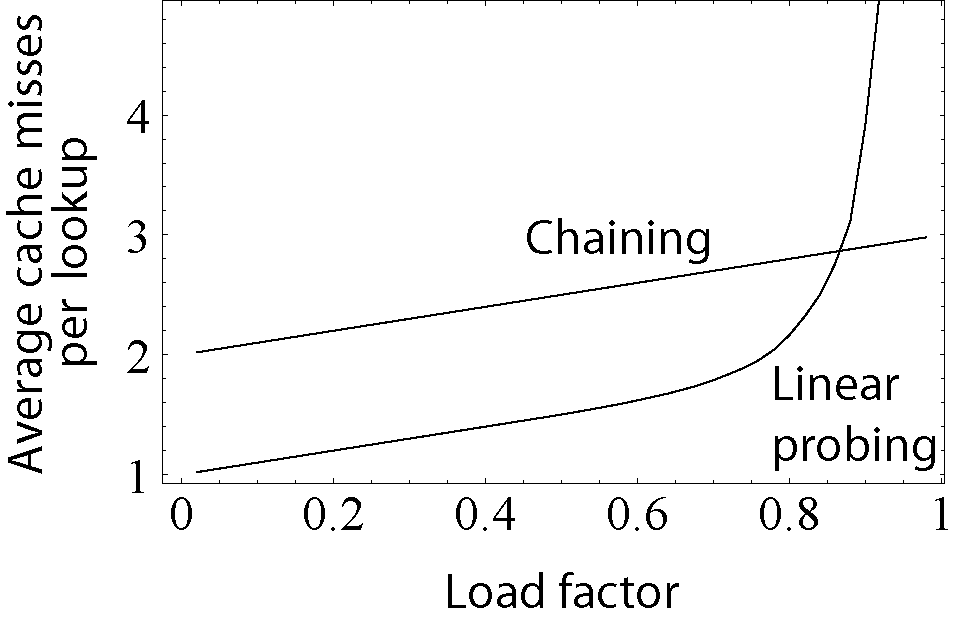
\includegraphics[width=1.0\textwidth,height=6.5in,keepaspectratio]{../images/40.png}
\end{center}
\raggedright{}\myfigurewithcaption{40}{This graph compares the average number of cache misses required to lookup elements in tables with chaining and linear probing. As the table passes the 80\%-{}full mark, linear probing\textquotesingle{}s performance drastically degrades.}
\end{minipage}\vspace{0.75cm}



For small record sizes (a few words or less) the benefits of in-{}place open addressing compared to chaining are:
\begin{myitemize}
\item{}  They can be more space-{}efficient than chaining since they don\textquotesingle{}t need to store any pointers or allocate any additional space outside the hash table. Simple linked lists require a word of overhead per element.
\item{}  Insertions avoid the time overhead of memory allocation, and can even be implemented in the absence of a memory allocator.
\item{}  Because it uses internal storage, open addressing avoids the extra indirection required for chaining\textquotesingle{}s external storage. It also has better \myhref{http://en.wikipedia.org/wiki/locality\%20of\%20reference}{locality of reference}, particularly with linear probing. With small record sizes, these factors can yield better performance than chaining, particularly for lookups.
\item{}  They can be easier to \myhref{http://en.wikipedia.org/wiki/serialization}{serialize}, because they don\textquotesingle{}t use pointers.
\end{myitemize}


On the other hand, normal open addressing is a poor choice for large elements, since these elements fill entire cache lines (negating the cache advantage), and a large amount of space is wasted on large empty table slots. If the open addressing table only stores references to elements (external storage), it uses space comparable to chaining even for large records but loses its speed advantage.

Generally speaking, open addressing is better used for hash tables with small records that can be stored within the table (internal storage) and fit in a cache line. They are particularly suitable for elements of one word or less. In cases where the tables are expected to have high load factors, the records are large, or the data is variable-{}sized, chained hash tables often perform as well or better.

Ultimately, used sensibly any kind of hash table algorithm is usually fast {\itshape enough} \setmainfont[Path=/usr/share/fonts/truetype/cmu/,UprightFont=cmunrm.ttf,BoldFont=cmunbx.ttf,ItalicFont=cmunti.ttf,BoldItalicFont=cmunbi.ttf]{cmunrm.ttf}\setmonofont[Path=/usr/share/fonts/truetype/cmu/,UprightFont=cmuntt.ttf,BoldFont=cmuntb.ttf,ItalicFont=cmunit.ttf,BoldItalicFont=cmuntx.ttf]{cmunrm.ttf}; and the percentage of a calculation spent in hash table code is low. Memory usage is rarely considered excessive. Therefore, in most cases the differences between these algorithms is marginal, and other considerations typically come into play.
\subsubsection{Coalesced hashing}
\label{121}
Main Page: \myhref{http://en.wikibooks.org/wiki/Coalesced\%20hashing}{Coalesced hashing}

A hybrid of chaining and open addressing, coalesced hashing links together chains of nodes within the table itself. Like open addressing, it achieves space usage and (somewhat diminished) cache advantages over chaining. Like chaining, it does not exhibit clustering effects; in fact, the table can be efficiently filled to a high density. Unlike chaining, it cannot have more elements than table slots.
\subsubsection{Perfect hashing}
\label{122}
Main Page: \myhref{http://en.wikibooks.org/wiki/Perfect\%20hashing}{Perfect hashing}

If all of the keys that will be used are known ahead of time, and there are no more keys that can fit the hash table, \myhref{http://en.wikibooks.org/wiki/perfect\%20hashing}{perfect hashing} can be used to create a perfect hash table, in which there will be no collisions. If \myhref{http://en.wikibooks.org/wiki/minimal\%20perfect\%20hashing}{minimal perfect hashing} is used, every location in the hash table can be used as well.

Perfect hashing gives a hash table where the time to make a lookup is constant in the worst case. This is in contrast to chaining and open addressing methods, where the time for lookup is low on average, but may be arbitrarily large. There exist methods for maintaining a perfect hash function under insertions of keys, known as \myhref{http://en.wikibooks.org/wiki/dynamic\%20perfect\%20hashing}{dynamic perfect hashing}. A simpler alternative, that also gives worst case constant lookup time, is \myhref{http://en.wikibooks.org/wiki/cuckoo\%20hashing}{cuckoo hashing}.
\subsubsection{Probabilistic hashing}
\label{123}
Perhaps the simplest solution to a collision is to replace the value that is already in the slot with the new value, or slightly less commonly, drop the record that is to be inserted. In later searches, this may result in a search not finding a record which has been inserted. This technique is particularly useful for implementing caching.

An even more space-{}efficient solution which is similar to this is use a \myhref{http://en.wikipedia.org/wiki/bit\%20array}{bit array} (an array of one-{}bit fields) for our table. Initially all bits are set to zero, and when we insert a key, we set the corresponding bit to one. False negatives cannot occur, but \myhref{http://en.wikibooks.org/wiki/false\%20positives}{false positives} can, since if the search finds a 1 bit, it will claim that the value was found, even if it was just another value that hashed into the same array slot by coincidence. In reality, such a hash table is merely a specific type of \myhref{http://en.wikipedia.org/wiki/Bloom\%20filter}{Bloom filter}.
\subsection{Table resizing}
\label{124}

With a good hash function, a hash table can typically contain about 70\%{\mbox{$-$}}80\% as many elements as it does table slots and still perform well. Depending on the collision resolution mechanism, performance can begin to suffer either gradually or dramatically as more elements are added. To deal with this, when the load factor exceeds some threshold, we allocate a new, larger table, and add all the contents of the original table to this new table. In \myhref{http://en.wikibooks.org/wiki/Java\%20programming\%20language}{Java}\textquotesingle{}s HashMap class, for example, the default load factor threshold is 0.75.

This can be a very expensive operation, and the necessity for it is one of the hash table\textquotesingle{}s disadvantages. In fact, some naive methods for doing this, such as enlarging the table by one each time you add a new element, reduce performance so drastically as to make the hash table useless. However, if we enlarge the table by some fixed percent, such as 10\% or 100\%, it can be shown using \myhref{http://en.wikibooks.org/wiki/amortized\%20analysis}{amortized analysis} that these resizings are so infrequent that the average time per lookup remains constant-{}time. To see why this is true, suppose a hash table using chaining begins at the minimum size of 1 and is doubled each time it fills above 100\%. If in the end it contains {\itshape n} \setmainfont[Path=/usr/share/fonts/truetype/cmu/,UprightFont=cmunrm.ttf,BoldFont=cmunbx.ttf,ItalicFont=cmunti.ttf,BoldItalicFont=cmunbi.ttf]{cmunrm.ttf}\setmonofont[Path=/usr/share/fonts/truetype/cmu/,UprightFont=cmuntt.ttf,BoldFont=cmuntb.ttf,ItalicFont=cmunit.ttf,BoldItalicFont=cmuntx.ttf]{cmunrm.ttf} elements, then the total add operations performed for all the resizings is:

\begin{myquote}
\item{} 1 + 2 + 4 + ... + {\itshape n} \setmainfont[Path=/usr/share/fonts/truetype/cmu/,UprightFont=cmunrm.ttf,BoldFont=cmunbx.ttf,ItalicFont=cmunti.ttf,BoldItalicFont=cmunbi.ttf]{cmunrm.ttf}\setmonofont[Path=/usr/share/fonts/truetype/cmu/,UprightFont=cmuntt.ttf,BoldFont=cmuntb.ttf,ItalicFont=cmunit.ttf,BoldItalicFont=cmuntx.ttf]{cmunrm.ttf} = 2{\itshape n} \setmainfont[Path=/usr/share/fonts/truetype/cmu/,UprightFont=cmunrm.ttf,BoldFont=cmunbx.ttf,ItalicFont=cmunti.ttf,BoldItalicFont=cmunbi.ttf]{cmunrm.ttf}\setmonofont[Path=/usr/share/fonts/truetype/cmu/,UprightFont=cmuntt.ttf,BoldFont=cmuntb.ttf,ItalicFont=cmunit.ttf,BoldItalicFont=cmuntx.ttf]{cmunrm.ttf} -{} 1.
\end{myquote}


Because the costs of the resizings form a \myhref{http://en.wikibooks.org/wiki/geometric\%20series}{geometric series}, the total cost is O({\itshape n} \setmainfont[Path=/usr/share/fonts/truetype/cmu/,UprightFont=cmunrm.ttf,BoldFont=cmunbx.ttf,ItalicFont=cmunti.ttf,BoldItalicFont=cmunbi.ttf]{cmunrm.ttf}\setmonofont[Path=/usr/share/fonts/truetype/cmu/,UprightFont=cmuntt.ttf,BoldFont=cmuntb.ttf,ItalicFont=cmunit.ttf,BoldItalicFont=cmuntx.ttf]{cmunrm.ttf}). But we also perform {\itshape n} \setmainfont[Path=/usr/share/fonts/truetype/cmu/,UprightFont=cmunrm.ttf,BoldFont=cmunbx.ttf,ItalicFont=cmunti.ttf,BoldItalicFont=cmunbi.ttf]{cmunrm.ttf}\setmonofont[Path=/usr/share/fonts/truetype/cmu/,UprightFont=cmuntt.ttf,BoldFont=cmuntb.ttf,ItalicFont=cmunit.ttf,BoldItalicFont=cmuntx.ttf]{cmunrm.ttf} operations to add the {\itshape n} \setmainfont[Path=/usr/share/fonts/truetype/cmu/,UprightFont=cmunrm.ttf,BoldFont=cmunbx.ttf,ItalicFont=cmunti.ttf,BoldItalicFont=cmunbi.ttf]{cmunrm.ttf}\setmonofont[Path=/usr/share/fonts/truetype/cmu/,UprightFont=cmuntt.ttf,BoldFont=cmuntb.ttf,ItalicFont=cmunit.ttf,BoldItalicFont=cmuntx.ttf]{cmunrm.ttf} elements in the first place, so the total time to add {\itshape n} \setmainfont[Path=/usr/share/fonts/truetype/cmu/,UprightFont=cmunrm.ttf,BoldFont=cmunbx.ttf,ItalicFont=cmunti.ttf,BoldItalicFont=cmunbi.ttf]{cmunrm.ttf}\setmonofont[Path=/usr/share/fonts/truetype/cmu/,UprightFont=cmuntt.ttf,BoldFont=cmuntb.ttf,ItalicFont=cmunit.ttf,BoldItalicFont=cmuntx.ttf]{cmunrm.ttf} elements with resizing is O({\itshape n} \setmainfont[Path=/usr/share/fonts/truetype/cmu/,UprightFont=cmunrm.ttf,BoldFont=cmunbx.ttf,ItalicFont=cmunti.ttf,BoldItalicFont=cmunbi.ttf]{cmunrm.ttf}\setmonofont[Path=/usr/share/fonts/truetype/cmu/,UprightFont=cmuntt.ttf,BoldFont=cmuntb.ttf,ItalicFont=cmunit.ttf,BoldItalicFont=cmuntx.ttf]{cmunrm.ttf}), an amortized time of O(1) per element.

On the other hand, some hash table implementations, notably in \myhref{http://en.wikibooks.org/wiki/real-time\%20system}{real-{}time system}s, cannot pay the price of enlarging the hash table all at once, because it may interrupt time-{}critical operations. One simple approach is to initially allocate the table with enough space for the expected number of elements and forbid the addition of too many elements. Another useful but more memory-{}intensive technique is to perform the resizing gradually:
\begin{myitemize}
\item{}  Allocate the new hash table, but leave the old hash table and check both tables during lookups.
\item{}  Each time an insertion is performed, add that element to the new table and also move {\itshape k} \setmainfont[Path=/usr/share/fonts/truetype/cmu/,UprightFont=cmunrm.ttf,BoldFont=cmunbx.ttf,ItalicFont=cmunti.ttf,BoldItalicFont=cmunbi.ttf]{cmunrm.ttf}\setmonofont[Path=/usr/share/fonts/truetype/cmu/,UprightFont=cmuntt.ttf,BoldFont=cmuntb.ttf,ItalicFont=cmunit.ttf,BoldItalicFont=cmuntx.ttf]{cmunrm.ttf} elements from the old table to the new table.
\item{}  When all elements are removed from the old table, deallocate it.
\end{myitemize}

To ensure that the old table will be completely copied over before the new table itself needs to be enlarged, it\textquotesingle{}s necessary to increase the size of the table by a factor of at least ({\itshape k} \setmainfont[Path=/usr/share/fonts/truetype/cmu/,UprightFont=cmunrm.ttf,BoldFont=cmunbx.ttf,ItalicFont=cmunti.ttf,BoldItalicFont=cmunbi.ttf]{cmunrm.ttf}\setmonofont[Path=/usr/share/fonts/truetype/cmu/,UprightFont=cmuntt.ttf,BoldFont=cmuntb.ttf,ItalicFont=cmunit.ttf,BoldItalicFont=cmuntx.ttf]{cmunrm.ttf} + 1)/{\itshape k} \setmainfont[Path=/usr/share/fonts/truetype/cmu/,UprightFont=cmunrm.ttf,BoldFont=cmunbx.ttf,ItalicFont=cmunti.ttf,BoldItalicFont=cmunbi.ttf]{cmunrm.ttf}\setmonofont[Path=/usr/share/fonts/truetype/cmu/,UprightFont=cmuntt.ttf,BoldFont=cmuntb.ttf,ItalicFont=cmunit.ttf,BoldItalicFont=cmuntx.ttf]{cmunrm.ttf} during the resizing.

\myhref{http://en.wikibooks.org/wiki/Linear\%20hashing}{Linear hashing} is a hash table algorithm that permits incremental hash table expansion.  It is implemented using a single hash table, but with two possible look-{}up functions.

Another way to decrease the cost of table resizing is to choose a hash function in such a way that the hashes of most values do not change when the table is resized. This approach, called \myhref{http://en.wikibooks.org/wiki/consistent\%20hashing}{consistent hashing}, is prevalent in disk-{}based and distributed hashes, where resizing is prohibitively costly.
\subsection{Ordered retrieval issue}
\label{125}
Hash tables store data in pseudo-{}random locations, so accessing the data in a sorted manner is a very time consuming operation. Other data structures such as \myhref{http://en.wikibooks.org/wiki/self-balancing\%20binary\%20search\%20tree}{self-{}balancing binary search tree}s generally operate more slowly (since their lookup time is O(log {\itshape n} \setmainfont[Path=/usr/share/fonts/truetype/cmu/,UprightFont=cmunrm.ttf,BoldFont=cmunbx.ttf,ItalicFont=cmunti.ttf,BoldItalicFont=cmunbi.ttf]{cmunrm.ttf}\setmonofont[Path=/usr/share/fonts/truetype/cmu/,UprightFont=cmuntt.ttf,BoldFont=cmuntb.ttf,ItalicFont=cmunit.ttf,BoldItalicFont=cmuntx.ttf]{cmunrm.ttf})) and are rather more complex to implement than hash tables but maintain a sorted data structure at all times. See \myhref{http://en.wikibooks.org/wiki/Associative_array\%23Efficient_representations}{a comparison of hash tables and self-{}balancing binary search trees}.
\subsection{Problems with hash tables}
\label{126}
Although hash table lookups use constant time on average, the time spent can be significant. Evaluating a good hash function can be a slow operation. In particular, if simple array indexing can be used instead, this is usually faster.

Hash tables in general exhibit poor \myhref{http://en.wikibooks.org/wiki/locality\%20of\%20reference}{locality of reference}{\mbox{$\text{---}$}}that is, the data to be accessed is distributed seemingly at random in memory. Because hash tables cause access patterns that jump around, this can trigger \myhref{http://en.wikibooks.org/wiki/CPU\%20cache}{microprocessor cache} misses that cause long delays. Compact data structures such as arrays, searched with \myhref{http://en.wikibooks.org/wiki/linear\%20search}{linear search}, may be faster if the table is relatively small and keys are cheap to compare, such as with simple integer keys. According to \myhref{http://en.wikibooks.org/wiki/Moore\%27s\%20Law}{Moore\textquotesingle{}s Law}, cache sizes are growing exponentially and so what is considered \symbol{34}small\symbol{34} may be increasing. The optimal performance point varies from system to system; for example, a trial on \myhref{http://en.wikibooks.org/wiki/Parrot\%20virtual\%20machine}{Parrot} shows that its hash tables outperform linear search in all but the most trivial cases (one to three entries).

More significantly, hash tables are more difficult and error-{}prone to write and use. Hash tables require the design of an effective hash function for each key type, which in many situations is more difficult and time-{}consuming to design and debug than the mere comparison function required for a \myhref{http://en.wikibooks.org/wiki/self-balancing\%20binary\%20search\%20tree}{self-{}balancing binary search tree}. In open-{}addressed hash tables it\textquotesingle{}s even easier to create a poor hash function.

Additionally, in some applications, a \myhref{http://en.wikibooks.org/wiki/black\%20hat}{black hat} with knowledge of the hash function may be able to supply information to a hash which creates worst-{}case behavior by causing excessive collisions, resulting in very poor performance (i.e., a \myhref{http://en.wikibooks.org/wiki/denial\%20of\%20service\%20attack}{denial of service attack}). In critical applications, either \myhref{http://en.wikibooks.org/wiki/universal\%20hashing}{universal hashing} can be used or a data structure with better worst-{}case guarantees may be preferable. For details, see Crosby and Wallach\textquotesingle{}s {\itshape \myhref{http://www.cs.rice.edu/~scrosby/hash/CrosbyWallach_UsenixSec2003.pdf}{\setmainfont[Path=/usr/share/fonts/truetype/cmu/,UprightFont=cmunrm.ttf,BoldFont=cmunbx.ttf,ItalicFont=cmunti.ttf,BoldItalicFont=cmunbi.ttf]{cmunti.ttf}\setmonofont[Path=/usr/share/fonts/truetype/cmu/,UprightFont=cmuntt.ttf,BoldFont=cmuntb.ttf,ItalicFont=cmunit.ttf,BoldItalicFont=cmuntx.ttf]{cmunti.ttf}\itshape Denial of Service via Algorithmic Complexity Attacks}} .
\subsection{Other hash table algorithms}
\label{127}
{\bfseries \setmainfont[Path=/usr/share/fonts/truetype/cmu/,UprightFont=cmunrm.ttf,BoldFont=cmunbx.ttf,ItalicFont=cmunti.ttf,BoldItalicFont=cmunbi.ttf]{cmunbx.ttf}\setmonofont[Path=/usr/share/fonts/truetype/cmu/,UprightFont=cmuntt.ttf,BoldFont=cmuntb.ttf,ItalicFont=cmunit.ttf,BoldItalicFont=cmuntx.ttf]{cmunbx.ttf}\bfseries Extendible hashing} \setmainfont[Path=/usr/share/fonts/truetype/cmu/,UprightFont=cmunrm.ttf,BoldFont=cmunbx.ttf,ItalicFont=cmunti.ttf,BoldItalicFont=cmunbi.ttf]{cmunrm.ttf}\setmonofont[Path=/usr/share/fonts/truetype/cmu/,UprightFont=cmuntt.ttf,BoldFont=cmuntb.ttf,ItalicFont=cmunit.ttf,BoldItalicFont=cmuntx.ttf]{cmunrm.ttf} and {\bfseries \setmainfont[Path=/usr/share/fonts/truetype/cmu/,UprightFont=cmunrm.ttf,BoldFont=cmunbx.ttf,ItalicFont=cmunti.ttf,BoldItalicFont=cmunbi.ttf]{cmunbx.ttf}\setmonofont[Path=/usr/share/fonts/truetype/cmu/,UprightFont=cmuntt.ttf,BoldFont=cmuntb.ttf,ItalicFont=cmunit.ttf,BoldItalicFont=cmuntx.ttf]{cmunbx.ttf}\bfseries linear hashing} \setmainfont[Path=/usr/share/fonts/truetype/cmu/,UprightFont=cmunrm.ttf,BoldFont=cmunbx.ttf,ItalicFont=cmunti.ttf,BoldItalicFont=cmunbi.ttf]{cmunrm.ttf}\setmonofont[Path=/usr/share/fonts/truetype/cmu/,UprightFont=cmuntt.ttf,BoldFont=cmuntb.ttf,ItalicFont=cmunit.ttf,BoldItalicFont=cmuntx.ttf]{cmunrm.ttf} are hash algorithms that are used in the context of database algorithms used for instance in index file structures, and even primary file organization for a database. Generally, in order to make search scalable for large databases, the search time should be proportional log N or near constant, where N is the number of records to search. Log N searches can be implemented with tree structures, because the degree of fan out and the shortness of the tree relates to the number of steps needed to find a record, so the height of the tree is the maximum number of disc accesses it takes to find where a record is.
However, hash tables are also used, because the cost of a disk access can be counted in units of disc accesses, and often that unit is a block of data. Since a hash table can, in the best case, find a key with one or two accesses, a hash table index is regarded as generally faster when retrieving a collection of records during a join operation e.g. \\

\TemplateSpaceIndent{$\text{ }${}SELECT$\text{ }${}*$\text{ }${}from$\text{ }${}customer,$\text{ }${}orders$\text{ }${}where$\text{ }${}customer.cust\_id$\text{ }${}=$\text{ }${}orders.cust\_id$\text{ }${}and$\text{ }$\newline{}
$\text{ }${}cust\_id$\text{ }${}=$\text{ }${}X}

i.e. If orders has a hash index on cust\_id, then it takes constant time to locate the block that contains record locations for orders matching cust\_id = X. (although, it would be better if the value type of orders was a list of order ids, so that hash keys are just one unique cust\_id for each batch of orders, to avoid unnecessary collisions). 

Extendible hashing and linear hashing have certain similarities: collisions are accepted as inevitable and are part of the algorithm where blocks or buckets of collision space is added ; traditional good hash function ranges are required, but the hash value is transformed by a dynamic address function : in {\bfseries \setmainfont[Path=/usr/share/fonts/truetype/cmu/,UprightFont=cmunrm.ttf,BoldFont=cmunbx.ttf,ItalicFont=cmunti.ttf,BoldItalicFont=cmunbi.ttf]{cmunbx.ttf}\setmonofont[Path=/usr/share/fonts/truetype/cmu/,UprightFont=cmuntt.ttf,BoldFont=cmuntb.ttf,ItalicFont=cmunit.ttf,BoldItalicFont=cmuntx.ttf]{cmunbx.ttf}\bfseries extendible hashing} \setmainfont[Path=/usr/share/fonts/truetype/cmu/,UprightFont=cmunrm.ttf,BoldFont=cmunbx.ttf,ItalicFont=cmunti.ttf,BoldItalicFont=cmunbi.ttf]{cmunrm.ttf}\setmonofont[Path=/usr/share/fonts/truetype/cmu/,UprightFont=cmuntt.ttf,BoldFont=cmuntb.ttf,ItalicFont=cmunit.ttf,BoldItalicFont=cmuntx.ttf]{cmunrm.ttf},
a bit mask is used to mask out unwanted bits, but this mask length increases by one periodically, doubling the
available addressing space ; also in extendible hashing, there is an indirection with a directory address space, the directory entries being paired with another address (a pointer ) to the actual block containing the key-{}value pairs; the entries in the directory correspond to the bit masked hash value (so that the number of entries is equal to maximum bit mask value + 1 e.g. a bit mask of 2 bits, can address a directory of 00 01 10 11, or 3 + 1 = 4).  

In {\bfseries \setmainfont[Path=/usr/share/fonts/truetype/cmu/,UprightFont=cmunrm.ttf,BoldFont=cmunbx.ttf,ItalicFont=cmunti.ttf,BoldItalicFont=cmunbi.ttf]{cmunbx.ttf}\setmonofont[Path=/usr/share/fonts/truetype/cmu/,UprightFont=cmuntt.ttf,BoldFont=cmuntb.ttf,ItalicFont=cmunit.ttf,BoldItalicFont=cmuntx.ttf]{cmunbx.ttf}\bfseries linear hashing} \setmainfont[Path=/usr/share/fonts/truetype/cmu/,UprightFont=cmunrm.ttf,BoldFont=cmunbx.ttf,ItalicFont=cmunti.ttf,BoldItalicFont=cmunbi.ttf]{cmunrm.ttf}\setmonofont[Path=/usr/share/fonts/truetype/cmu/,UprightFont=cmuntt.ttf,BoldFont=cmuntb.ttf,ItalicFont=cmunit.ttf,BoldItalicFont=cmuntx.ttf]{cmunrm.ttf}, the traditional hash value is also masked with a bit mask, but
if the resultant smaller hash value falls below a \textquotesingle{}split\textquotesingle{} variable, the original hash value is masked with
a bit mask of one bit greater length, making the resultant hash value address recently added blocks. The split variable ranges incrementally between 0 and the maximum current bit mask value e.g. a bit mask of 2, or in the terminology of linear hashing, a \symbol{34}level\symbol{34} of 2, the split variable will range between 0 to 3. When the split variable reaches 4, the level increases by 1, so in the next round of the split variable, it will range between 0 to 7, and reset again when it reaches 8. 

The split variable incrementally allows increased addressing space, as new blocks are added; the decision to add a new block occurs whenever a key-{}and=value is being inserted, and overflows the particular block the key-{}and-{}value\textquotesingle{}s key hashes into. This overflow location may be completely unrelated to the block going to be split pointed to by the split variable. However, over time, it is expected that given a good random hash function that distributes entries fairly evenly amongst all addressable blocks,
the blocks that actually require splitting because they have overflowed get their turn in round-{}robin fashion as the split value ranges between 0 -{} N where N has a factor of 2 to the power of Level, level being the variable incremented whenever the split variable hits N. 

New blocks are added one at a time with both extendible hashing, and with linear hashing.

In {\bfseries \setmainfont[Path=/usr/share/fonts/truetype/cmu/,UprightFont=cmunrm.ttf,BoldFont=cmunbx.ttf,ItalicFont=cmunti.ttf,BoldItalicFont=cmunbi.ttf]{cmunbx.ttf}\setmonofont[Path=/usr/share/fonts/truetype/cmu/,UprightFont=cmuntt.ttf,BoldFont=cmuntb.ttf,ItalicFont=cmunit.ttf,BoldItalicFont=cmuntx.ttf]{cmunbx.ttf}\bfseries extendible hashing} \setmainfont[Path=/usr/share/fonts/truetype/cmu/,UprightFont=cmunrm.ttf,BoldFont=cmunbx.ttf,ItalicFont=cmunti.ttf,BoldItalicFont=cmunbi.ttf]{cmunrm.ttf}\setmonofont[Path=/usr/share/fonts/truetype/cmu/,UprightFont=cmuntt.ttf,BoldFont=cmuntb.ttf,ItalicFont=cmunit.ttf,BoldItalicFont=cmuntx.ttf]{cmunrm.ttf},  a block overflow ( a new key-{}value colliding with B other key-{}values, where B is the size of a block) is handled by checking the size of the bit mask \symbol{34}locally\symbol{34}, called the \symbol{34}local depth\symbol{34}, an attribute which must be stored with the block. The directory structure, also has a depth, the \symbol{34}global depth\symbol{34}. If the local depth is less than the global depth, then the local depth is incremented, and all the key values are rehashed and passed through a bit mask which is one bit longer now, placing them either in the current block, or in another block. 
If the other block happens to be the same block when looked up in the directory, a new block is added, and the directory entry for the other block is made to point to the new block. Why does the directory have entries where two entries point to the same block ? This is because if the local depth {\bfseries \setmainfont[Path=/usr/share/fonts/truetype/cmu/,UprightFont=cmunrm.ttf,BoldFont=cmunbx.ttf,ItalicFont=cmunti.ttf,BoldItalicFont=cmunbi.ttf]{cmunbx.ttf}\setmonofont[Path=/usr/share/fonts/truetype/cmu/,UprightFont=cmuntt.ttf,BoldFont=cmuntb.ttf,ItalicFont=cmunit.ttf,BoldItalicFont=cmuntx.ttf]{cmunbx.ttf}\bfseries is equal to} \setmainfont[Path=/usr/share/fonts/truetype/cmu/,UprightFont=cmunrm.ttf,BoldFont=cmunbx.ttf,ItalicFont=cmunti.ttf,BoldItalicFont=cmunbi.ttf]{cmunrm.ttf}\setmonofont[Path=/usr/share/fonts/truetype/cmu/,UprightFont=cmuntt.ttf,BoldFont=cmuntb.ttf,ItalicFont=cmunit.ttf,BoldItalicFont=cmuntx.ttf]{cmunrm.ttf}  the global depth of the directory, this means the bit mask of the directory does not have enough bits to deal with an increment in the bit mask length of the block, and so the directory must have its bit mask length incremented, but this means the directory now doubles the number of addressable entries. Since half the entries addressable don\textquotesingle{}t exist, the directory simply copies the pointers over to the new entries e.g. if the directory had entries for 00, 01, 10, 11, or a 2 bit mask, and it becomes a 3 bit mask, then 000 001 010 011 100 101 110 111 become the new entries, and  00\textquotesingle{}s block address go to 000 and 001 ; 01\textquotesingle{}s pointer goes to 010 and 011, 10 goes to 100 and 101 and so on.  And so this creates the situation where two directory entries point to the same block. Although the block that was going to overflow, now can add a new block by redirecting the second pointer to a newly appended block, the other original blocks will have two pointers to them. When it is their turn to split, the algorithm will check local vs global depth and this time find that the local depth is less, and hence no directory splitting is required, only a new block be appended, and the second directory pointer moved from addressing the previous block to addressing the new block.

In {\bfseries \setmainfont[Path=/usr/share/fonts/truetype/cmu/,UprightFont=cmunrm.ttf,BoldFont=cmunbx.ttf,ItalicFont=cmunti.ttf,BoldItalicFont=cmunbi.ttf]{cmunbx.ttf}\setmonofont[Path=/usr/share/fonts/truetype/cmu/,UprightFont=cmuntt.ttf,BoldFont=cmuntb.ttf,ItalicFont=cmunit.ttf,BoldItalicFont=cmuntx.ttf]{cmunbx.ttf}\bfseries linear hashing} \setmainfont[Path=/usr/share/fonts/truetype/cmu/,UprightFont=cmunrm.ttf,BoldFont=cmunbx.ttf,ItalicFont=cmunti.ttf,BoldItalicFont=cmunbi.ttf]{cmunrm.ttf}\setmonofont[Path=/usr/share/fonts/truetype/cmu/,UprightFont=cmuntt.ttf,BoldFont=cmuntb.ttf,ItalicFont=cmunit.ttf,BoldItalicFont=cmuntx.ttf]{cmunrm.ttf}, adding a similarly hashed block does not occurs  immediately when a block overflows, and therefore an overflow block is created to be attached to the overflowing block. However, a block overflow is a signal that more space will be required, and this happens by splitting the block pointed to by the \symbol{34}split\symbol{34} variable, which is initially zero, and hence initially points to block zero. The splitting is done by taking all the key-{}value pairs in the
splitting block, and its overflow block(s), hashing the keys again, but with a bit mask of length current level + 1. This will result in
two block addresses, some will be the old block number, and others will be\\

\TemplateSpaceIndent{$\text{ }${}a2$\text{ }${}=$\text{ }${}old$\text{ }${}block$\text{ }${}number$\text{ }${}+$\text{ }${}($\text{ }${}N$\text{ }${}times$\text{ }${}2$\text{ }${}\^{}$\text{ }${}(level)$\text{ }${})}

{\bfseries
\begin{mydescription}Rationale
\end{mydescription}
}

Let m  = N times 2 \^{} level ; if h is the original hash value, and old block number = h mod m, and now the new block number is h mod ( m * 2 ), because m * 2 = N times 2 \^{} (level+1), then the new block number is either h mod m if (h / m) is even so dividing h/m by 2 leaves a zero remainder and therefore doesn\textquotesingle{}t change the remainder, or the new block number is ( h mod m )  + m because h / m is an odd number, and dividing h / m by 2 will leave an excess remainder of m, + the original remainder. ( The same rationale applies to extendible hashing depth incrementing ).

As above, a new block is created with a number a2, which will usually occur at +1 the previous a2 value. 
Once this is done, the split variable is incremented, so that the next a2 value will be again old a2 + 1. In this way, each block is covered by the split variable eventually, so each block is preemptively rehashed into extra space, and new blocks are added incrementally. Overflow blocks that are no longer needed are discarded, for later garbage collection if needed, or put on an available free block list by chaining.  

When the split variable reaches ( N times 2 \^{} level ), level is incremented and split variable is reset to zero. 
In this next round, the split variable will now traverse from zero to ( N times 2 \^{} (old\_level + 1 ) ), 
which is exactly the number of blocks at the start of the previous round, but including all the blocks created by the previous round.
\subsubsection{A simple inference on file storage mapping of linear hashing and extendible hashing}
\label{128}
As can be seen, extendible hashing requires space to store a directory which can double in size. 

Since the space of both algorithms increase by one block at a time, if blocks have a known maximum size or fixed size, then it is straight forward to map the blocks as blocks sequentially appended to a file. 

In extendible hashing, it would  be logical to store the directory as a separate file, as doubling can be accommodated by adding to the end of the directory file. The separate block file would not have to change, other than have blocks appended to its end. 

Header information for linear hashing doesn\textquotesingle{}t increase in size :  basically just the values for 
N, level, and split need to be recorded, so these can be incorporated as a header into a fixed block size linear hash storage file.

However, linear hashing requires space for overflow blocks, and this might best be stored in another file,
otherwise addressing blocks in the linear hash file is not as straight forward as multiplying the block number by the block size and adding the space for N,level, and split. 


In the next section, a complete example of linear hashing in Java is given, using a in memory implementation of linear hashing, and code to manage blocks as files in a file directory, the whole contents of the file directory representing the persistent linear hashing structure.
\subsection{Implementations}
\label{129}
While many programming languages already provide hash table functionality,\myfootnote{
\myfnhref{http://en.wikipedia.org/wiki/\%20Comparison\%20of\%20programming\%20languages\%20\%28mapping\%29}{Wikipedia: Comparison of programming languages (mapping)} shows how many programming languages provide hash table functionality.
}
there are several independent implementations worth mentioning.
\begin{myitemize}
\item{}  \myhref{http://goog-sparsehash.sourceforge.net/}{Google Sparse Hash} The Google SparseHash project contains several hash-{}map implementations in use at Google, with different performance characteristics, including an implementation that optimizes for space and one that optimizes for speed. The memory-{}optimized one is extremely memory-{}efficient with only 2 bits/entry of overhead.
\item{}  \myhref{https://launchpad.net/libmct}{MCT} provides hashtables similar to Google\textquotesingle{}s {\ttfamily \setmainfont[Path=/usr/share/fonts/truetype/cmu/,UprightFont=cmunrm.ttf,BoldFont=cmunbx.ttf,ItalicFont=cmunti.ttf,BoldItalicFont=cmunbi.ttf]{cmuntt.ttf}\setmonofont[Path=/usr/share/fonts/truetype/cmu/,UprightFont=cmuntt.ttf,BoldFont=cmuntb.ttf,ItalicFont=cmunit.ttf,BoldItalicFont=cmuntx.ttf]{cmuntt.ttf}\ttfamily dense\_hash\_map} \setmainfont[Path=/usr/share/fonts/truetype/cmu/,UprightFont=cmunrm.ttf,BoldFont=cmunbx.ttf,ItalicFont=cmunti.ttf,BoldItalicFont=cmunbi.ttf]{cmunrm.ttf}\setmonofont[Path=/usr/share/fonts/truetype/cmu/,UprightFont=cmuntt.ttf,BoldFont=cmuntb.ttf,ItalicFont=cmunit.ttf,BoldItalicFont=cmuntx.ttf]{cmunrm.ttf}, but without restriction on contained values; it also comes with exception safety and support for C++0x features.
\item{}  A number of runtime languages and/or standard libraries use hash tables to implement their support for associative arrays because of their efficiency.
\end{myitemize}

\subsubsection{A python implementation of extendible hashing}
\label{130}
The file -{} block management routines aren\textquotesingle{}t there, so this could be added in to make this a real implementation of a database hash index.

A full page is split according to the (local depth)th bit, first by collecting all the directory indices pointing to the full page, updating the pointers according to
the d bit being 0 or 1 corresponding to first and second new pages, then reloading all the key-{}values after hashing each key and using the d bit of each hash to see which page to allocate to. The local depth of each new page is one greater than the old page\textquotesingle{}s local depth, so that the next d bit can be used next time when splitting.


\begin{Shaded}
\begin{Highlighting}[]

\NormalTok{PAGE_SZ\ensuremath{\text{ }}=\ensuremath{\text{ }}}\DecValTok{20}\newline
\ensuremath{\text{ }}\newline
\KeywordTok{class}\ensuremath{\text{ }}\NormalTok{Page:}\newline
\ensuremath{\text{ }}\newline
	\KeywordTok{def}\ensuremath{\text{ }}\OtherTok{__init__}\NormalTok{(}\OtherTok{self}\NormalTok{):}\newline
		\OtherTok{self}\NormalTok{.m\ensuremath{\text{ }}=\ensuremath{\text{ }}\{\}}\newline
		\OtherTok{self}\NormalTok{.d\ensuremath{\text{ }}=\ensuremath{\text{ }}}\DecValTok{0}\newline
		\newline
	\KeywordTok{def}\ensuremath{\text{ }}\NormalTok{full(}\OtherTok{self}\NormalTok{):}\newline
		\KeywordTok{return}\ensuremath{\text{ }}\DataTypeTok{len}\NormalTok{(}\OtherTok{self}\NormalTok{.m)\ensuremath{\text{ }}>\ensuremath{\text{ }}PAGE_SZ\ensuremath{\text{ }}}\newline
\ensuremath{\text{ }}\newline
	\KeywordTok{def}\ensuremath{\text{ }}\NormalTok{put(}\OtherTok{self}\NormalTok{,k,v):}\newline
		\OtherTok{self}\NormalTok{.m[k]\ensuremath{\text{ }}=\ensuremath{\text{ }}v}\newline
\ensuremath{\text{ }}\newline
	\KeywordTok{def}\ensuremath{\text{ }}\NormalTok{get(}\OtherTok{self}\NormalTok{,k):}\newline
		\KeywordTok{return}\ensuremath{\text{ }}\OtherTok{self}\NormalTok{.m.get(k)}\newline
\ensuremath{\text{ }}\newline
\KeywordTok{class}\ensuremath{\text{ }}\NormalTok{EH:}\newline
\ensuremath{\text{ }}\newline
	\KeywordTok{def}\ensuremath{\text{ }}\OtherTok{__init__}\NormalTok{(}\OtherTok{self}\NormalTok{):}\newline
		\OtherTok{self}\NormalTok{.gd\ensuremath{\text{ }}=\ensuremath{\text{ }}}\DecValTok{0}\ensuremath{\text{ }}\newline
		\NormalTok{p\ensuremath{\text{ }}=\ensuremath{\text{ }}Page()}\newline
		\OtherTok{self}\NormalTok{.pp=\ensuremath{\text{ }}[p]}\newline
\ensuremath{\text{ }}\newline
	\KeywordTok{def}\ensuremath{\text{ }}\NormalTok{get_page(}\OtherTok{self}\NormalTok{,k):}\newline
		\NormalTok{h\ensuremath{\text{ }}=\ensuremath{\text{ }}}\DataTypeTok{hash}\NormalTok{(k)\ensuremath{\text{ }}}\newline
		\NormalTok{p\ensuremath{\text{ }}=\ensuremath{\text{ }}}\OtherTok{self}\NormalTok{.pp[\ensuremath{\text{ }}h\ensuremath{\text{ }}\&\ensuremath{\text{ }}((\ensuremath{\text{ }}}\DecValTok{1}\ensuremath{\text{ }}\NormalTok{<<\ensuremath{\text{ }}}\OtherTok{self}\NormalTok{.gd)\ensuremath{\text{ }}-}\DecValTok{1}\NormalTok{)]}\newline
		\KeywordTok{return}\ensuremath{\text{ }}\NormalTok{p		}\newline
\ensuremath{\text{ }}\newline
	\KeywordTok{def}\ensuremath{\text{ }}\ensuremath{\text{ }}\NormalTok{put(}\OtherTok{self}\NormalTok{,\ensuremath{\text{ }}k,\ensuremath{\text{ }}v):}\newline
		\NormalTok{p\ensuremath{\text{ }}=\ensuremath{\text{ }}}\OtherTok{self}\NormalTok{.get_page(k)}\newline
		\KeywordTok{if}\ensuremath{\text{ }}\NormalTok{p.full()\ensuremath{\text{ }}and\ensuremath{\text{ }}p.d\ensuremath{\text{ }}==\ensuremath{\text{ }}}\OtherTok{self}\NormalTok{.gd:}\newline
			\OtherTok{self}\NormalTok{.pp\ensuremath{\text{ }}=\ensuremath{\text{ }}}\OtherTok{self}\NormalTok{.pp\ensuremath{\text{ }}+\ensuremath{\text{ }}}\OtherTok{self}\NormalTok{.pp}\newline
			\OtherTok{self}\NormalTok{.gd\ensuremath{\text{ }}+=\ensuremath{\text{ }}}\DecValTok{1}\newline
	\newline
		\newline
		\KeywordTok{if}\ensuremath{\text{ }}\NormalTok{p.full()\ensuremath{\text{ }}and\ensuremath{\text{ }}p.d\ensuremath{\text{ }}<\ensuremath{\text{ }}}\OtherTok{self}\NormalTok{.gd:}\newline
			\NormalTok{p.put(k,v);}\newline
			\NormalTok{p1\ensuremath{\text{ }}=\ensuremath{\text{ }}Page()}\newline
			\NormalTok{p2\ensuremath{\text{ }}=\ensuremath{\text{ }}Page()}\newline
			\KeywordTok{for}\ensuremath{\text{ }}\NormalTok{k2\ensuremath{\text{ }}in\ensuremath{\text{ }}p.m.keys():}\newline
				\NormalTok{v2\ensuremath{\text{ }}=\ensuremath{\text{ }}p.m[k2]}\newline
				\NormalTok{h\ensuremath{\text{ }}=\ensuremath{\text{ }}k2.}\OtherTok{__hash__}\NormalTok{()}\newline
				\NormalTok{h\ensuremath{\text{ }}=\ensuremath{\text{ }}h\ensuremath{\text{ }}\&\ensuremath{\text{ }}((}\DecValTok{1}\ensuremath{\text{ }}\NormalTok{<<\ensuremath{\text{ }}}\OtherTok{self}\NormalTok{.gd)\ensuremath{\text{ }}-}\DecValTok{1}\NormalTok{)}\newline
				\KeywordTok{if}\ensuremath{\text{ }}\NormalTok{(h\ensuremath{\text{ }}|\ensuremath{\text{ }}(}\DecValTok{1}\ensuremath{\text{ }}\NormalTok{<<\ensuremath{\text{ }}p.d)\ensuremath{\text{ }}==\ensuremath{\text{ }}h):}\newline
					\NormalTok{p2.put(k2,v2)}\newline
				\KeywordTok{else}\NormalTok{:}\newline
					\NormalTok{p1.put(k2,v2)}\newline
			\NormalTok{l\ensuremath{\text{ }}=\ensuremath{\text{ }}[]}\newline
			\KeywordTok{for}\ensuremath{\text{ }}\NormalTok{i\ensuremath{\text{ }}in\ensuremath{\text{ }}}\DataTypeTok{xrange}\NormalTok{(}\DecValTok{0}\NormalTok{,\ensuremath{\text{ }}}\DataTypeTok{len}\NormalTok{(}\OtherTok{self}\NormalTok{.pp)):}\newline
				\KeywordTok{if}\ensuremath{\text{ }}\OtherTok{self}\NormalTok{.pp[i]\ensuremath{\text{ }}==\ensuremath{\text{ }}p:}\newline
					\NormalTok{l.append(i)}\newline
			\KeywordTok{for}\ensuremath{\text{ }}\NormalTok{i\ensuremath{\text{ }}in\ensuremath{\text{ }}l:}\newline
				\KeywordTok{if}\ensuremath{\text{ }}\NormalTok{(i\ensuremath{\text{ }}|\ensuremath{\text{ }}(\ensuremath{\text{ }}}\DecValTok{1}\ensuremath{\text{ }}\NormalTok{<<\ensuremath{\text{ }}p.d)\ensuremath{\text{ }}==\ensuremath{\text{ }}i):}\newline
					\OtherTok{self}\NormalTok{.pp[i]\ensuremath{\text{ }}=\ensuremath{\text{ }}p2}\newline
					\newline
				\KeywordTok{else}\NormalTok{:}\newline
					\OtherTok{self}\NormalTok{.pp[i]\ensuremath{\text{ }}=\ensuremath{\text{ }}p1}\newline
\ensuremath{\text{ }}\newline
			\NormalTok{p1.d\ensuremath{\text{ }}=\ensuremath{\text{ }}p.d\ensuremath{\text{ }}+\ensuremath{\text{ }}}\DecValTok{1}\newline
			\NormalTok{p2.d\ensuremath{\text{ }}=\ensuremath{\text{ }}p1.d}\newline
		\KeywordTok{else}\NormalTok{:	}\newline
			\NormalTok{p.put(k,\ensuremath{\text{ }}\ensuremath{\text{ }}v)}\newline
\ensuremath{\text{ }}\newline
	\KeywordTok{def}\ensuremath{\text{ }}\NormalTok{get(}\OtherTok{self}\NormalTok{,\ensuremath{\text{ }}k):}\newline
		\NormalTok{p\ensuremath{\text{ }}=\ensuremath{\text{ }}}\OtherTok{self}\NormalTok{.get_page(k)}\newline
		\KeywordTok{return}\ensuremath{\text{ }}\NormalTok{p.get(k)}\newline
\ensuremath{\text{ }}\newline
		\newline
\ensuremath{\text{ }}\newline
\KeywordTok{if}\ensuremath{\text{ }}\OtherTok{__name__}\ensuremath{\text{ }}\NormalTok{==\ensuremath{\text{ }}}\StringTok{"__main__"}\NormalTok{:}\newline
	\NormalTok{eh\ensuremath{\text{ }}=\ensuremath{\text{ }}EH()}\newline
	\NormalTok{N\ensuremath{\text{ }}=\ensuremath{\text{ }}}\DecValTok{10000}\newline
	\NormalTok{l\ensuremath{\text{ }}=\ensuremath{\text{ }}[]}\newline
	\KeywordTok{for}\ensuremath{\text{ }}\NormalTok{i\ensuremath{\text{ }}in\ensuremath{\text{ }}}\DataTypeTok{range}\NormalTok{(}\DecValTok{0}\NormalTok{,N):	}\newline
		\NormalTok{l.append(i)}\newline
\ensuremath{\text{ }}\newline
	\CharTok{import}\ensuremath{\text{ }}\NormalTok{random}\newline
	\NormalTok{random.shuffle(l)}\newline
	\KeywordTok{for}\ensuremath{\text{ }}\NormalTok{i\ensuremath{\text{ }}in\ensuremath{\text{ }}l:}\newline
		\NormalTok{eh.put(i,i)}\newline
	\DataTypeTok{print}\ensuremath{\text{ }}\NormalTok{l}\newline
\ensuremath{\text{ }}\newline
	\KeywordTok{for}\ensuremath{\text{ }}\NormalTok{i\ensuremath{\text{ }}in\ensuremath{\text{ }}}\DataTypeTok{range}\NormalTok{(}\DecValTok{0}\NormalTok{,\ensuremath{\text{ }}N):}\newline
		\DataTypeTok{print}\ensuremath{\text{ }}\NormalTok{eh.get(i)}\newline
\ensuremath{\text{ }}\newline
\end{Highlighting}
\end{Shaded}

\subsubsection{A Java implementation of extendible hashing}
\label{131}
A direct Java translation of the above python code, tested to work.


\begin{Shaded}
\begin{Highlighting}[]

\KeywordTok{package\ensuremath{\text{ }}ext_hashing;}\newline
\ensuremath{\text{ }}\newline
\KeywordTok{import\ensuremath{\text{ }}java.util.ArrayList;}\newline
\KeywordTok{import\ensuremath{\text{ }}java.util.HashMap;}\newline
\KeywordTok{import\ensuremath{\text{ }}java.util.List;}\newline
\KeywordTok{import\ensuremath{\text{ }}java.util.Map;}\newline
\KeywordTok{import\ensuremath{\text{ }}java.util.Random;}\newline
\ensuremath{\text{ }}\newline
\KeywordTok{public}\ensuremath{\text{ }}\KeywordTok{class}\ensuremath{\text{ }}\NormalTok{EH2<K,\ensuremath{\text{ }}V>\ensuremath{\text{ }}\{}\newline
	\DataTypeTok{static}\ensuremath{\text{ }}\KeywordTok{class}\ensuremath{\text{ }}\NormalTok{Page<K,\ensuremath{\text{ }}V>\ensuremath{\text{ }}\{}\newline
		\DataTypeTok{static}\ensuremath{\text{ }}\DataTypeTok{int}\ensuremath{\text{ }}\NormalTok{PAGE_SZ\ensuremath{\text{ }}=\ensuremath{\text{ }}}\DecValTok{20}\NormalTok{;}\newline
		\KeywordTok{private}\ensuremath{\text{ }}\NormalTok{Map<K,\ensuremath{\text{ }}V>\ensuremath{\text{ }}m\ensuremath{\text{ }}=\ensuremath{\text{ }}}\KeywordTok{new}\ensuremath{\text{ }}\NormalTok{HashMap<K,\ensuremath{\text{ }}V>();}\newline
		\DataTypeTok{int}\ensuremath{\text{ }}\NormalTok{d\ensuremath{\text{ }}=\ensuremath{\text{ }}}\DecValTok{0}\NormalTok{;}\newline
\ensuremath{\text{ }}\newline
		\DataTypeTok{boolean}\ensuremath{\text{ }}\FunctionTok{full}\NormalTok{()\ensuremath{\text{ }}\{}\newline
			\KeywordTok{return}\ensuremath{\text{ }}\NormalTok{m.}\FunctionTok{size}\NormalTok{()\ensuremath{\text{ }}>\ensuremath{\text{ }}PAGE_SZ;}\newline
		\NormalTok{\}}\newline
\ensuremath{\text{ }}\newline
		\DataTypeTok{void}\ensuremath{\text{ }}\FunctionTok{put}\NormalTok{(K\ensuremath{\text{ }}k,\ensuremath{\text{ }}V\ensuremath{\text{ }}v)\ensuremath{\text{ }}\{}\newline
			\NormalTok{m.}\FunctionTok{put}\NormalTok{(k,\ensuremath{\text{ }}v);}\newline
\ensuremath{\text{ }}\newline
		\NormalTok{\}}\newline
\ensuremath{\text{ }}\newline
		\NormalTok{V\ensuremath{\text{ }}}\FunctionTok{get}\NormalTok{(K\ensuremath{\text{ }}k)\ensuremath{\text{ }}\{}\newline
			\KeywordTok{return}\ensuremath{\text{ }}\NormalTok{m.}\FunctionTok{get}\NormalTok{(k);}\newline
		\NormalTok{\}}\newline
	\NormalTok{\}}\newline
\ensuremath{\text{ }}\newline
	\DataTypeTok{int}\ensuremath{\text{ }}\NormalTok{gd\ensuremath{\text{ }}=\ensuremath{\text{ }}}\DecValTok{0}\NormalTok{;}\newline
\ensuremath{\text{ }}\newline
	\NormalTok{List<Page<K,\ensuremath{\text{ }}V>>\ensuremath{\text{ }}pp\ensuremath{\text{ }}=\ensuremath{\text{ }}}\KeywordTok{new}\ensuremath{\text{ }}\NormalTok{ArrayList<Page<K,\ensuremath{\text{ }}V>>();}\newline
\ensuremath{\text{ }}\newline
	\KeywordTok{public}\ensuremath{\text{ }}\FunctionTok{EH2}\NormalTok{()\ensuremath{\text{ }}\{}\newline
		\NormalTok{pp.}\FunctionTok{add}\NormalTok{(}\KeywordTok{new}\ensuremath{\text{ }}\NormalTok{Page<K,\ensuremath{\text{ }}V>());}\newline
	\NormalTok{\}}\newline
\ensuremath{\text{ }}\newline
	\NormalTok{Page<K,\ensuremath{\text{ }}V>\ensuremath{\text{ }}}\FunctionTok{getPage}\NormalTok{(K\ensuremath{\text{ }}k)\ensuremath{\text{ }}\{}\newline
		\DataTypeTok{int}\ensuremath{\text{ }}\NormalTok{h\ensuremath{\text{ }}=\ensuremath{\text{ }}k.}\FunctionTok{hashCode}\NormalTok{();}\newline
		\NormalTok{Page<K,\ensuremath{\text{ }}V>\ensuremath{\text{ }}p\ensuremath{\text{ }}=\ensuremath{\text{ }}pp.}\FunctionTok{get}\NormalTok{(h\ensuremath{\text{ }}\&\ensuremath{\text{ }}((}\DecValTok{1}\ensuremath{\text{ }}\NormalTok{<<\ensuremath{\text{ }}gd)\ensuremath{\text{ }}-\ensuremath{\text{ }}}\DecValTok{1}\NormalTok{));}\newline
		\KeywordTok{return}\ensuremath{\text{ }}\NormalTok{p;}\newline
	\NormalTok{\}}\newline
\ensuremath{\text{ }}\newline
	\DataTypeTok{void}\ensuremath{\text{ }}\FunctionTok{put}\NormalTok{(K\ensuremath{\text{ }}k,\ensuremath{\text{ }}V\ensuremath{\text{ }}v)\ensuremath{\text{ }}\{}\newline
		\NormalTok{Page<K,\ensuremath{\text{ }}V>\ensuremath{\text{ }}p\ensuremath{\text{ }}=\ensuremath{\text{ }}}\FunctionTok{getPage}\NormalTok{(k);}\newline
		\KeywordTok{if}\ensuremath{\text{ }}\NormalTok{(p.}\FunctionTok{full}\NormalTok{()\ensuremath{\text{ }}\&\&\ensuremath{\text{ }}p.}\FunctionTok{d}\ensuremath{\text{ }}\NormalTok{==\ensuremath{\text{ }}gd)\ensuremath{\text{ }}\{}\newline
			\NormalTok{List<Page<K,\ensuremath{\text{ }}V>>\ensuremath{\text{ }}pp2\ensuremath{\text{ }}=\ensuremath{\text{ }}}\KeywordTok{new}\ensuremath{\text{ }}\NormalTok{ArrayList<EH2.}\FunctionTok{Page}\NormalTok{<K,\ensuremath{\text{ }}V>>(pp);}\newline
			\NormalTok{pp.}\FunctionTok{addAll}\NormalTok{(pp2);}\newline
			\NormalTok{++gd;}\newline
		\NormalTok{\}}\newline
\ensuremath{\text{ }}\newline
		\KeywordTok{if}\ensuremath{\text{ }}\NormalTok{(p.}\FunctionTok{full}\NormalTok{()\ensuremath{\text{ }}\&\&\ensuremath{\text{ }}p.}\FunctionTok{d}\ensuremath{\text{ }}\NormalTok{<\ensuremath{\text{ }}gd)\ensuremath{\text{ }}\{}\newline
			\NormalTok{p.}\FunctionTok{put}\NormalTok{(k,\ensuremath{\text{ }}v);}\newline
			\NormalTok{Page<K,\ensuremath{\text{ }}V>\ensuremath{\text{ }}p1,\ensuremath{\text{ }}p2;}\newline
			\NormalTok{p1\ensuremath{\text{ }}=\ensuremath{\text{ }}}\KeywordTok{new}\ensuremath{\text{ }}\NormalTok{Page<K,\ensuremath{\text{ }}V>();}\newline
			\NormalTok{p2\ensuremath{\text{ }}=\ensuremath{\text{ }}}\KeywordTok{new}\ensuremath{\text{ }}\NormalTok{Page<K,\ensuremath{\text{ }}V>();}\newline
			\KeywordTok{for}\ensuremath{\text{ }}\NormalTok{(K\ensuremath{\text{ }}k2\ensuremath{\text{ }}:\ensuremath{\text{ }}p.}\FunctionTok{m}\NormalTok{.}\FunctionTok{keySet}\NormalTok{())\ensuremath{\text{ }}\{}\newline
				\NormalTok{V\ensuremath{\text{ }}v2\ensuremath{\text{ }}=\ensuremath{\text{ }}p.}\FunctionTok{m}\NormalTok{.}\FunctionTok{get}\NormalTok{(k2);}\newline
\ensuremath{\text{ }}\newline
				\DataTypeTok{int}\ensuremath{\text{ }}\NormalTok{h\ensuremath{\text{ }}=\ensuremath{\text{ }}k2.}\FunctionTok{hashCode}\NormalTok{()\ensuremath{\text{ }}\&\ensuremath{\text{ }}((}\DecValTok{1}\ensuremath{\text{ }}\NormalTok{<<\ensuremath{\text{ }}gd)\ensuremath{\text{ }}-\ensuremath{\text{ }}}\DecValTok{1}\NormalTok{);}\newline
\ensuremath{\text{ }}\newline
				\KeywordTok{if}\ensuremath{\text{ }}\NormalTok{((h\ensuremath{\text{ }}|\ensuremath{\text{ }}(}\DecValTok{1}\ensuremath{\text{ }}\NormalTok{<<\ensuremath{\text{ }}p.}\FunctionTok{d}\NormalTok{))\ensuremath{\text{ }}==\ensuremath{\text{ }}h)}\newline
					\NormalTok{p2.}\FunctionTok{put}\NormalTok{(k2,\ensuremath{\text{ }}v2);}\newline
				\KeywordTok{else}\newline
					\NormalTok{p1.}\FunctionTok{put}\NormalTok{(k2,\ensuremath{\text{ }}v2);}\newline
			\NormalTok{\}}\newline
\ensuremath{\text{ }}\newline
			\NormalTok{List<Integer>\ensuremath{\text{ }}l\ensuremath{\text{ }}=\ensuremath{\text{ }}}\KeywordTok{new}\ensuremath{\text{ }}\NormalTok{ArrayList<Integer>();}\newline
\ensuremath{\text{ }}\newline
			\KeywordTok{for}\ensuremath{\text{ }}\NormalTok{(}\DataTypeTok{int}\ensuremath{\text{ }}\NormalTok{i\ensuremath{\text{ }}=\ensuremath{\text{ }}}\DecValTok{0}\NormalTok{;\ensuremath{\text{ }}i\ensuremath{\text{ }}<\ensuremath{\text{ }}pp.}\FunctionTok{size}\NormalTok{();\ensuremath{\text{ }}++i)}\newline
				\KeywordTok{if}\ensuremath{\text{ }}\NormalTok{(pp.}\FunctionTok{get}\NormalTok{(i)\ensuremath{\text{ }}==\ensuremath{\text{ }}p)}\newline
					\NormalTok{l.}\FunctionTok{add}\NormalTok{(i);}\newline
\ensuremath{\text{ }}\newline
			\KeywordTok{for}\ensuremath{\text{ }}\NormalTok{(}\DataTypeTok{int}\ensuremath{\text{ }}\NormalTok{i\ensuremath{\text{ }}:\ensuremath{\text{ }}l)}\newline
				\KeywordTok{if}\ensuremath{\text{ }}\NormalTok{((i\ensuremath{\text{ }}|\ensuremath{\text{ }}(}\DecValTok{1}\ensuremath{\text{ }}\NormalTok{<<\ensuremath{\text{ }}p.}\FunctionTok{d}\NormalTok{))\ensuremath{\text{ }}==\ensuremath{\text{ }}i)}\newline
					\NormalTok{pp.}\FunctionTok{set}\NormalTok{(i,\ensuremath{\text{ }}p2);}\newline
				\KeywordTok{else}\newline
					\NormalTok{pp.}\FunctionTok{set}\NormalTok{(i,\ensuremath{\text{ }}p1);}\newline
\ensuremath{\text{ }}\newline
			\NormalTok{p1.}\FunctionTok{d}\ensuremath{\text{ }}\NormalTok{=\ensuremath{\text{ }}p.}\FunctionTok{d}\ensuremath{\text{ }}\NormalTok{+\ensuremath{\text{ }}}\DecValTok{1}\NormalTok{;}\newline
			\NormalTok{p2.}\FunctionTok{d}\ensuremath{\text{ }}\NormalTok{=\ensuremath{\text{ }}p1.}\FunctionTok{d}\NormalTok{;}\newline
\ensuremath{\text{ }}\newline
		\NormalTok{\}\ensuremath{\text{ }}}\KeywordTok{else}\newline
			\NormalTok{p.}\FunctionTok{put}\NormalTok{(k,\ensuremath{\text{ }}v);}\newline
	\NormalTok{\}}\newline
\ensuremath{\text{ }}\newline
	\KeywordTok{public}\ensuremath{\text{ }}\NormalTok{V\ensuremath{\text{ }}}\FunctionTok{get}\NormalTok{(K\ensuremath{\text{ }}k)\ensuremath{\text{ }}\{}\newline
		\KeywordTok{return}\ensuremath{\text{ }}\FunctionTok{getPage}\NormalTok{(k).}\FunctionTok{get}\NormalTok{(k);}\newline
	\NormalTok{\}}\newline
\ensuremath{\text{ }}\newline
	\KeywordTok{public}\ensuremath{\text{ }}\DataTypeTok{static}\ensuremath{\text{ }}\DataTypeTok{void}\ensuremath{\text{ }}\FunctionTok{main}\NormalTok{(String[]\ensuremath{\text{ }}args)\ensuremath{\text{ }}\{}\newline
\ensuremath{\text{ }}\newline
		\DataTypeTok{int}\ensuremath{\text{ }}\NormalTok{N\ensuremath{\text{ }}=\ensuremath{\text{ }}}\DecValTok{500000}\NormalTok{;}\newline
\ensuremath{\text{ }}\newline
		\NormalTok{Random\ensuremath{\text{ }}r\ensuremath{\text{ }}=\ensuremath{\text{ }}}\KeywordTok{new}\ensuremath{\text{ }}\NormalTok{Random();}\newline
		\NormalTok{List<Integer>\ensuremath{\text{ }}l\ensuremath{\text{ }}=\ensuremath{\text{ }}}\KeywordTok{new}\ensuremath{\text{ }}\NormalTok{ArrayList<Integer>();}\newline
		\KeywordTok{for}\ensuremath{\text{ }}\NormalTok{(}\DataTypeTok{int}\ensuremath{\text{ }}\NormalTok{i\ensuremath{\text{ }}=\ensuremath{\text{ }}}\DecValTok{0}\NormalTok{;\ensuremath{\text{ }}i\ensuremath{\text{ }}<\ensuremath{\text{ }}N;\ensuremath{\text{ }}++i)\ensuremath{\text{ }}\{}\newline
			\NormalTok{l.}\FunctionTok{add}\NormalTok{(i);}\newline
		\NormalTok{\}}\newline
\ensuremath{\text{ }}\newline
		\KeywordTok{for}\ensuremath{\text{ }}\NormalTok{(}\DataTypeTok{int}\ensuremath{\text{ }}\NormalTok{i\ensuremath{\text{ }}=\ensuremath{\text{ }}}\DecValTok{0}\NormalTok{;\ensuremath{\text{ }}i\ensuremath{\text{ }}<\ensuremath{\text{ }}N;\ensuremath{\text{ }}++i)\ensuremath{\text{ }}\{}\newline
			\DataTypeTok{int}\ensuremath{\text{ }}\NormalTok{j\ensuremath{\text{ }}=\ensuremath{\text{ }}r.}\FunctionTok{nextInt}\NormalTok{(N);}\newline
			\DataTypeTok{int}\ensuremath{\text{ }}\NormalTok{t\ensuremath{\text{ }}=\ensuremath{\text{ }}l.}\FunctionTok{get}\NormalTok{(j);}\newline
			\NormalTok{l.}\FunctionTok{set}\NormalTok{(j,\ensuremath{\text{ }}l.}\FunctionTok{get}\NormalTok{(i));}\newline
			\NormalTok{l.}\FunctionTok{set}\NormalTok{(i,\ensuremath{\text{ }}t);}\newline
		\NormalTok{\}}\newline
\ensuremath{\text{ }}\newline
		\NormalTok{EH2<Integer,\ensuremath{\text{ }}Integer>\ensuremath{\text{ }}eh\ensuremath{\text{ }}=\ensuremath{\text{ }}}\KeywordTok{new}\ensuremath{\text{ }}\NormalTok{EH2<Integer,\ensuremath{\text{ }}Integer>();}\newline
		\KeywordTok{for}\ensuremath{\text{ }}\NormalTok{(}\DataTypeTok{int}\ensuremath{\text{ }}\NormalTok{i\ensuremath{\text{ }}=\ensuremath{\text{ }}}\DecValTok{0}\NormalTok{;\ensuremath{\text{ }}i\ensuremath{\text{ }}<\ensuremath{\text{ }}N;\ensuremath{\text{ }}++i)\ensuremath{\text{ }}\{}\newline
			\NormalTok{eh.}\FunctionTok{put}\NormalTok{(l.}\FunctionTok{get}\NormalTok{(i),\ensuremath{\text{ }}l.}\FunctionTok{get}\NormalTok{(i));}\newline
		\NormalTok{\}}\newline
\ensuremath{\text{ }}\newline
		\KeywordTok{for}\ensuremath{\text{ }}\NormalTok{(}\DataTypeTok{int}\ensuremath{\text{ }}\NormalTok{i\ensuremath{\text{ }}=\ensuremath{\text{ }}}\DecValTok{0}\NormalTok{;\ensuremath{\text{ }}i\ensuremath{\text{ }}<\ensuremath{\text{ }}N;\ensuremath{\text{ }}++i)\ensuremath{\text{ }}\{}\newline
			\NormalTok{System.}\FunctionTok{out.printf}\NormalTok{(}\StringTok{"}\CharTok{\%d}\StringTok{:}\CharTok{\%d}\StringTok{\ensuremath{\text{ }},\ensuremath{\text{ }}"}\NormalTok{,\ensuremath{\text{ }}i,\ensuremath{\text{ }}eh.}\FunctionTok{get}\NormalTok{(i));}\newline
			\KeywordTok{if}\ensuremath{\text{ }}\NormalTok{(i\ensuremath{\text{ }}\%\ensuremath{\text{ }}}\DecValTok{10}\ensuremath{\text{ }}\NormalTok{==\ensuremath{\text{ }}}\DecValTok{0}\NormalTok{)}\newline
				\NormalTok{System.}\FunctionTok{out}\NormalTok{.}\FunctionTok{println}\NormalTok{();}\newline
		\NormalTok{\}}\newline
\ensuremath{\text{ }}\newline
	\NormalTok{\}}\newline
\NormalTok{\}}\newline
\ensuremath{\text{ }}\newline
\end{Highlighting}
\end{Shaded}

\subsubsection{A Java implementation of linear hashing}
\label{132}
( usable for simple database indexing of arbitrary size, (almost ?) )

This code evolved out of a need for a bigger Java HashMap. Originally, a Java HashMap standard object was used as a Map
to index a heap like database file ( DBF format). But then, a file was encountered with so many records that the OutOfMemoryError
was being thrown, so linear hashing seemed like a reasonably simple algorithm to use as a disk based index scheme. 

Initially, linear hashing was implemented behind the Java Map interface, mainly the put(k,v) and get(k,v) methods. Generics was used, in order
not to get too involved in the key and value details. 
\subparagraph{debugging to achieve functionality}
{$\text{ }$}\newline\label{133}
Custom dumps to System.err was used to verify that blocks were being created, filled, and overflow blocks were of expected number if they existed ( no. = 1 ).
This was all done in a purely in-{}memory implementation.

Later, the standard Java decoupling was introduced, where the original LHMap2 class accepted listeners to events, such as when a block was needed. The listener was then implemented as a block file manager, loading blocks into the block list of the memory LHMap2 object whenever a null block was encountered on the block list,
and checking whether virtual machine runtime free memory was low, and retiring blocks using just a basic first-{}to-{}last-{}listed cache removal algorithm
(not least recently used (LRU), not least often used ) by saving them to disk file, and then actively invoking the system garbage collector.

Because an application use case existed, which was to externally index a large DBF table, this use case was used as the main test harness for the algorithm implementation.


\begin{Shaded}
\begin{Highlighting}[]

\KeywordTok{package\ensuremath{\text{ }}linearhashmap;}\newline
\ensuremath{\text{ }}\newline
\KeywordTok{import\ensuremath{\text{ }}java.io.Externalizable;}\newline
\KeywordTok{import\ensuremath{\text{ }}java.io.IOException;}\newline
\KeywordTok{import\ensuremath{\text{ }}java.io.ObjectInput;}\newline
\KeywordTok{import\ensuremath{\text{ }}java.io.ObjectOutput;}\newline
\KeywordTok{import\ensuremath{\text{ }}java.io.Serializable;}\newline
\KeywordTok{import\ensuremath{\text{ }}java.util.ArrayList;}\newline
\KeywordTok{import\ensuremath{\text{ }}java.util.Collection;}\newline
\KeywordTok{import\ensuremath{\text{ }}java.util.Iterator;}\newline
\KeywordTok{import\ensuremath{\text{ }}java.util.LinkedList;}\newline
\KeywordTok{import\ensuremath{\text{ }}java.util.List;}\newline
\KeywordTok{import\ensuremath{\text{ }}java.util.Map;}\newline
\KeywordTok{import\ensuremath{\text{ }}java.util.Set;}\newline
\KeywordTok{import\ensuremath{\text{ }}java.util.TreeMap;}\newline
\KeywordTok{import\ensuremath{\text{ }}java.util.TreeSet;}\newline
\ensuremath{\text{ }}\newline
\CommentTok{/**}\newline
\CommentTok{\ensuremath{\text{ }}*\ensuremath{\text{ }}}\newline
\CommentTok{\ensuremath{\text{ }}*\ensuremath{\text{ }}}\KeywordTok{@param\ensuremath{\text{ }}<K>}\newline
\CommentTok{\ensuremath{\text{ }}*\ensuremath{\text{ }}\ensuremath{\text{ }}\ensuremath{\text{ }}\ensuremath{\text{ }}\ensuremath{\text{ }}\ensuremath{\text{ }}\ensuremath{\text{ }}\ensuremath{\text{ }}\ensuremath{\text{ }}\ensuremath{\text{ }}\ensuremath{\text{ }}\ensuremath{\text{ }}key\ensuremath{\text{ }}type\ensuremath{\text{ }},\ensuremath{\text{ }}must\ensuremath{\text{ }}implement\ensuremath{\text{ }}equals()\ensuremath{\text{ }}and\ensuremath{\text{ }}hashCode()}\newline
\CommentTok{\ensuremath{\text{ }}*\ensuremath{\text{ }}}\KeywordTok{@param\ensuremath{\text{ }}<V>}\newline
\CommentTok{\ensuremath{\text{ }}*\ensuremath{\text{ }}\ensuremath{\text{ }}\ensuremath{\text{ }}\ensuremath{\text{ }}\ensuremath{\text{ }}\ensuremath{\text{ }}\ensuremath{\text{ }}\ensuremath{\text{ }}\ensuremath{\text{ }}\ensuremath{\text{ }}\ensuremath{\text{ }}\ensuremath{\text{ }}value\ensuremath{\text{ }}type}\newline
\CommentTok{\ensuremath{\text{ }}*\ensuremath{\text{ }}}\newline
\CommentTok{\ensuremath{\text{ }}*\ensuremath{\text{ }}}\newline
\CommentTok{\ensuremath{\text{ }}*/}\newline
\KeywordTok{public}\ensuremath{\text{ }}\KeywordTok{class}\ensuremath{\text{ }}\NormalTok{LHMap2<K,\ensuremath{\text{ }}V>\ensuremath{\text{ }}}\KeywordTok{implements}\ensuremath{\text{ }}\NormalTok{Map<K,\ensuremath{\text{ }}V>,\ensuremath{\text{ }}Serializable\ensuremath{\text{ }}\{}\newline
\ensuremath{\text{ }}\newline
	\CommentTok{/**}\newline
\CommentTok{	\ensuremath{\text{ }}*\ensuremath{\text{ }}}\newline
\CommentTok{	\ensuremath{\text{ }}*/}\newline
	\KeywordTok{private}\ensuremath{\text{ }}\DataTypeTok{static}\ensuremath{\text{ }}\DataTypeTok{final}\ensuremath{\text{ }}\DataTypeTok{long}\ensuremath{\text{ }}\NormalTok{serialVersionUID\ensuremath{\text{ }}=\ensuremath{\text{ }}3095071852466632996L;}\newline
\ensuremath{\text{ }}\newline
	\CommentTok{/**}\newline
\CommentTok{	\ensuremath{\text{ }}*\ensuremath{\text{ }}}\newline
\CommentTok{	\ensuremath{\text{ }}*/}\newline
\ensuremath{\text{ }}\newline
	\KeywordTok{public}\ensuremath{\text{ }}\DataTypeTok{static}\ensuremath{\text{ }}\KeywordTok{interface}\ensuremath{\text{ }}\NormalTok{BlockListener<K,\ensuremath{\text{ }}V>\ensuremath{\text{ }}\{}\newline
		\KeywordTok{public}\ensuremath{\text{ }}\DataTypeTok{void}\ensuremath{\text{ }}\FunctionTok{blockRequested}\NormalTok{(}\DataTypeTok{int}\ensuremath{\text{ }}\NormalTok{block,\ensuremath{\text{ }}LHMap2<K,\ensuremath{\text{ }}V>\ensuremath{\text{ }}map);}\newline
	\NormalTok{\}}\newline
\ensuremath{\text{ }}\newline
	\NormalTok{List<BlockListener<K,\ensuremath{\text{ }}V>>\ensuremath{\text{ }}listeners\ensuremath{\text{ }}=\ensuremath{\text{ }}}\KeywordTok{new}\ensuremath{\text{ }}\NormalTok{ArrayList<BlockListener<K,\ensuremath{\text{ }}V>>();}\newline
\ensuremath{\text{ }}\newline
	\CommentTok{//\ensuremath{\text{ }}int\ensuremath{\text{ }}savedBlocks;}\newline
	\DataTypeTok{int}\ensuremath{\text{ }}\NormalTok{N;}\newline
	\DataTypeTok{int}\ensuremath{\text{ }}\NormalTok{level\ensuremath{\text{ }}=\ensuremath{\text{ }}}\DecValTok{0}\NormalTok{;}\newline
	\DataTypeTok{int}\ensuremath{\text{ }}\NormalTok{split\ensuremath{\text{ }}=\ensuremath{\text{ }}}\DecValTok{0}\NormalTok{;}\newline
	\DataTypeTok{int}\ensuremath{\text{ }}\NormalTok{blockSize;}\newline
	\DataTypeTok{long}\ensuremath{\text{ }}\NormalTok{totalWrites\ensuremath{\text{ }}=\ensuremath{\text{ }}}\DecValTok{0}\NormalTok{;}\newline
\ensuremath{\text{ }}\newline
	\NormalTok{List<Block<K,\ensuremath{\text{ }}V>>\ensuremath{\text{ }}blockList\ensuremath{\text{ }}=\ensuremath{\text{ }}}\KeywordTok{new}\ensuremath{\text{ }}\NormalTok{ArrayList<Block<K,\ensuremath{\text{ }}V>>();}\newline
\ensuremath{\text{ }}\newline
	\KeywordTok{public}\ensuremath{\text{ }}\DataTypeTok{void}\ensuremath{\text{ }}\FunctionTok{addBlockListener}\NormalTok{(BlockListener<K,\ensuremath{\text{ }}V>\ensuremath{\text{ }}listener)\ensuremath{\text{ }}\{}\newline
		\NormalTok{listeners.}\FunctionTok{add}\NormalTok{(listener);}\newline
	\NormalTok{\}}\newline
\ensuremath{\text{ }}\newline
	\DataTypeTok{void}\ensuremath{\text{ }}\FunctionTok{notifyBlockRequested}\NormalTok{(}\DataTypeTok{int}\ensuremath{\text{ }}\NormalTok{block)\ensuremath{\text{ }}\{}\newline
		\KeywordTok{for}\ensuremath{\text{ }}\NormalTok{(BlockListener<K,\ensuremath{\text{ }}V>\ensuremath{\text{ }}l\ensuremath{\text{ }}:\ensuremath{\text{ }}listeners)\ensuremath{\text{ }}\{}\newline
			\NormalTok{l.}\FunctionTok{blockRequested}\NormalTok{(block,\ensuremath{\text{ }}}\KeywordTok{this}\NormalTok{);}\newline
		\NormalTok{\}}\newline
	\NormalTok{\}}\newline
\ensuremath{\text{ }}\newline
	\KeywordTok{public}\ensuremath{\text{ }}\FunctionTok{LHMap2}\NormalTok{(}\DataTypeTok{int}\ensuremath{\text{ }}\NormalTok{blockSize,\ensuremath{\text{ }}}\DataTypeTok{int}\ensuremath{\text{ }}\NormalTok{nStartingBlocks)\ensuremath{\text{ }}\{}\newline
		\KeywordTok{this}\NormalTok{.}\FunctionTok{blockSize}\ensuremath{\text{ }}\NormalTok{=\ensuremath{\text{ }}blockSize;}\newline
		\KeywordTok{this}\NormalTok{.}\FunctionTok{N}\ensuremath{\text{ }}\NormalTok{=\ensuremath{\text{ }}nStartingBlocks;}\newline
		\KeywordTok{for}\ensuremath{\text{ }}\NormalTok{(}\DataTypeTok{int}\ensuremath{\text{ }}\NormalTok{i\ensuremath{\text{ }}=\ensuremath{\text{ }}}\DecValTok{0}\NormalTok{;\ensuremath{\text{ }}i\ensuremath{\text{ }}<\ensuremath{\text{ }}nStartingBlocks;\ensuremath{\text{ }}++i)\ensuremath{\text{ }}\{}\newline
			\FunctionTok{addBlock}\NormalTok{();}\newline
		\NormalTok{\}}\newline
\ensuremath{\text{ }}\newline
		\NormalTok{Runtime.}\FunctionTok{getRuntime}\NormalTok{().}\FunctionTok{addShutdownHook}\NormalTok{(}\KeywordTok{new}\ensuremath{\text{ }}\NormalTok{Thread(}\KeywordTok{new}\ensuremath{\text{ }}\NormalTok{Runnable()\ensuremath{\text{ }}\{}\newline
\ensuremath{\text{ }}\newline
			\FunctionTok{@Override}\newline
			\KeywordTok{public}\ensuremath{\text{ }}\DataTypeTok{void}\ensuremath{\text{ }}\FunctionTok{run}\NormalTok{()\ensuremath{\text{ }}\{}\newline
				\FunctionTok{showStructure}\NormalTok{();}\newline
\ensuremath{\text{ }}\newline
			\NormalTok{\}}\newline
		\NormalTok{\}));}\newline
	\NormalTok{\}}\newline
\ensuremath{\text{ }}\newline
	\KeywordTok{public}\ensuremath{\text{ }}\DataTypeTok{static}\ensuremath{\text{ }}\KeywordTok{class}\ensuremath{\text{ }}\NormalTok{Block<K,\ensuremath{\text{ }}V>\ensuremath{\text{ }}}\KeywordTok{implements}\ensuremath{\text{ }}\NormalTok{Externalizable\ensuremath{\text{ }}\{}\newline
		\CommentTok{/**}\newline
\CommentTok{		\ensuremath{\text{ }}*\ensuremath{\text{ }}}\newline
\CommentTok{		\ensuremath{\text{ }}*/}\newline
\ensuremath{\text{ }}\newline
		\DataTypeTok{int}\ensuremath{\text{ }}\NormalTok{j\ensuremath{\text{ }}=\ensuremath{\text{ }}}\DecValTok{0}\NormalTok{;}\newline
\ensuremath{\text{ }}\newline
		\NormalTok{Block<K,\ensuremath{\text{ }}V>\ensuremath{\text{ }}overflow\ensuremath{\text{ }}=\ensuremath{\text{ }}}\KeywordTok{null}\NormalTok{;}\newline
		\NormalTok{LinkedList<K>\ensuremath{\text{ }}keyList\ensuremath{\text{ }}=\ensuremath{\text{ }}}\KeywordTok{new}\ensuremath{\text{ }}\NormalTok{LinkedList<K>();}\newline
		\NormalTok{LinkedList<V>\ensuremath{\text{ }}valueList\ensuremath{\text{ }}=\ensuremath{\text{ }}}\KeywordTok{new}\ensuremath{\text{ }}\NormalTok{LinkedList<V>();}\newline
		\KeywordTok{transient}\ensuremath{\text{ }}\KeywordTok{private}\ensuremath{\text{ }}\NormalTok{LHMap2<K,\ensuremath{\text{ }}V>\ensuremath{\text{ }}owner;}\newline
		\KeywordTok{transient}\ensuremath{\text{ }}\KeywordTok{private}\ensuremath{\text{ }}\NormalTok{Map<K,\ensuremath{\text{ }}V>\ensuremath{\text{ }}shadow\ensuremath{\text{ }}=\ensuremath{\text{ }}}\KeywordTok{new}\ensuremath{\text{ }}\NormalTok{TreeMap<K,\ensuremath{\text{ }}V>();}\newline
\ensuremath{\text{ }}\newline
		\KeywordTok{private}\ensuremath{\text{ }}\DataTypeTok{boolean}\ensuremath{\text{ }}\NormalTok{changed\ensuremath{\text{ }}=\ensuremath{\text{ }}}\KeywordTok{false}\NormalTok{;}\newline
\ensuremath{\text{ }}\newline
		\KeywordTok{private}\ensuremath{\text{ }}\DataTypeTok{int}\ensuremath{\text{ }}\NormalTok{size\ensuremath{\text{ }}=\ensuremath{\text{ }}}\DecValTok{0}\NormalTok{;}\newline
\ensuremath{\text{ }}\newline
		\KeywordTok{public}\ensuremath{\text{ }}\NormalTok{LHMap2<K,\ensuremath{\text{ }}V>\ensuremath{\text{ }}}\FunctionTok{getOwner}\NormalTok{()\ensuremath{\text{ }}\{}\newline
			\KeywordTok{return}\ensuremath{\text{ }}\NormalTok{owner;}\newline
		\NormalTok{\}}\newline
\ensuremath{\text{ }}\newline
		\KeywordTok{public}\ensuremath{\text{ }}\DataTypeTok{void}\ensuremath{\text{ }}\FunctionTok{setOwner}\NormalTok{(LHMap2<K,\ensuremath{\text{ }}V>\ensuremath{\text{ }}owner)\ensuremath{\text{ }}\{}\newline
			\KeywordTok{this}\NormalTok{.}\FunctionTok{owner}\ensuremath{\text{ }}\NormalTok{=\ensuremath{\text{ }}owner;}\newline
			\NormalTok{Block<K,\ensuremath{\text{ }}V>\ensuremath{\text{ }}ov\ensuremath{\text{ }}=\ensuremath{\text{ }}overflow;}\newline
			\KeywordTok{while}\ensuremath{\text{ }}\NormalTok{(ov\ensuremath{\text{ }}!=\ensuremath{\text{ }}}\KeywordTok{null}\NormalTok{)\ensuremath{\text{ }}\{}\newline
				\NormalTok{overflow.}\FunctionTok{setOwner}\NormalTok{(owner);}\newline
				\NormalTok{ov\ensuremath{\text{ }}=\ensuremath{\text{ }}ov.}\FunctionTok{overflow}\NormalTok{;}\newline
			\NormalTok{\}}\newline
		\NormalTok{\}}\newline
\ensuremath{\text{ }}\newline
		\KeywordTok{public}\ensuremath{\text{ }}\FunctionTok{Block}\NormalTok{()\ensuremath{\text{ }}\{}\newline
			\KeywordTok{super}\NormalTok{();}\newline
		\NormalTok{\}}\newline
\ensuremath{\text{ }}\newline
		\KeywordTok{public}\ensuremath{\text{ }}\FunctionTok{Block}\NormalTok{(LHMap2<K,\ensuremath{\text{ }}V>\ensuremath{\text{ }}map)\ensuremath{\text{ }}\{}\newline
			\FunctionTok{setOwner}\NormalTok{(map);}\newline
		\NormalTok{\}}\newline
\ensuremath{\text{ }}\newline
		\KeywordTok{public}\ensuremath{\text{ }}\NormalTok{V\ensuremath{\text{ }}}\FunctionTok{put}\NormalTok{(K\ensuremath{\text{ }}k,\ensuremath{\text{ }}V\ensuremath{\text{ }}v)\ensuremath{\text{ }}\{}\newline
			\FunctionTok{setChanged}\NormalTok{(}\KeywordTok{true}\NormalTok{);}\newline
\ensuremath{\text{ }}\newline
			\NormalTok{V\ensuremath{\text{ }}v2\ensuremath{\text{ }}=\ensuremath{\text{ }}}\FunctionTok{replace}\NormalTok{(k,\ensuremath{\text{ }}v);}\newline
			\KeywordTok{if}\ensuremath{\text{ }}\NormalTok{(v2\ensuremath{\text{ }}==\ensuremath{\text{ }}}\KeywordTok{null}\NormalTok{)\ensuremath{\text{ }}\{}\newline
				\NormalTok{++size;}\newline
				\KeywordTok{if}\ensuremath{\text{ }}\NormalTok{(keyList.}\FunctionTok{size}\NormalTok{()\ensuremath{\text{ }}==\ensuremath{\text{ }}}\FunctionTok{getOwner}\NormalTok{().}\FunctionTok{blockSize}\NormalTok{)\ensuremath{\text{ }}\{}\newline
\ensuremath{\text{ }}\newline
					\KeywordTok{if}\ensuremath{\text{ }}\NormalTok{(overflow\ensuremath{\text{ }}==\ensuremath{\text{ }}}\KeywordTok{null}\NormalTok{)\ensuremath{\text{ }}\{}\newline
						\FunctionTok{getOwner}\NormalTok{().}\FunctionTok{blockOverflowed}\NormalTok{(}\KeywordTok{this}\NormalTok{,\ensuremath{\text{ }}k,\ensuremath{\text{ }}v);}\newline
					\NormalTok{\}\ensuremath{\text{ }}}\KeywordTok{else}\ensuremath{\text{ }}\NormalTok{\{}\newline
						\NormalTok{overflow.}\FunctionTok{put}\NormalTok{(k,\ensuremath{\text{ }}v);}\newline
					\NormalTok{\}}\newline
\ensuremath{\text{ }}\newline
				\NormalTok{\}\ensuremath{\text{ }}}\KeywordTok{else}\ensuremath{\text{ }}\NormalTok{\{}\newline
					\NormalTok{keyList.}\FunctionTok{addFirst}\NormalTok{(k);}\newline
					\NormalTok{valueList.}\FunctionTok{addFirst}\NormalTok{(v);}\newline
				\NormalTok{\}}\newline
\ensuremath{\text{ }}\newline
			\NormalTok{\}}\newline
\ensuremath{\text{ }}\newline
			\KeywordTok{return}\ensuremath{\text{ }}\NormalTok{v2;}\newline
		\NormalTok{\}}\newline
\ensuremath{\text{ }}\newline
		\DataTypeTok{void}\ensuremath{\text{ }}\FunctionTok{setChanged}\NormalTok{(}\DataTypeTok{boolean}\ensuremath{\text{ }}\NormalTok{b)\ensuremath{\text{ }}\{}\newline
			\NormalTok{changed\ensuremath{\text{ }}=\ensuremath{\text{ }}b;}\newline
		\NormalTok{\}}\newline
\ensuremath{\text{ }}\newline
		\KeywordTok{public}\ensuremath{\text{ }}\NormalTok{Map<K,\ensuremath{\text{ }}V>\ensuremath{\text{ }}}\FunctionTok{drainToMap}\NormalTok{(Map<K,\ensuremath{\text{ }}V>\ensuremath{\text{ }}map)\ensuremath{\text{ }}\{}\newline
\ensuremath{\text{ }}\newline
			\KeywordTok{while}\ensuremath{\text{ }}\NormalTok{(!keyList.}\FunctionTok{isEmpty}\NormalTok{())\ensuremath{\text{ }}\{}\newline
				\NormalTok{K\ensuremath{\text{ }}k\ensuremath{\text{ }}=\ensuremath{\text{ }}keyList.}\FunctionTok{removeLast}\NormalTok{();}\newline
				\NormalTok{V\ensuremath{\text{ }}v\ensuremath{\text{ }}=\ensuremath{\text{ }}valueList.}\FunctionTok{removeLast}\NormalTok{();}\newline
				\NormalTok{map.}\FunctionTok{put}\NormalTok{(k,\ensuremath{\text{ }}v);}\newline
\ensuremath{\text{ }}\newline
			\NormalTok{\}}\newline
\ensuremath{\text{ }}\newline
			\KeywordTok{if}\ensuremath{\text{ }}\NormalTok{(overflow\ensuremath{\text{ }}!=\ensuremath{\text{ }}}\KeywordTok{null}\NormalTok{)}\newline
\ensuremath{\text{ }}\newline
				\NormalTok{map\ensuremath{\text{ }}=\ensuremath{\text{ }}overflow.}\FunctionTok{drainToMap}\NormalTok{(map);}\newline
\ensuremath{\text{ }}\newline
			\FunctionTok{garbageCollectionOverflow}\NormalTok{();}\newline
\ensuremath{\text{ }}\newline
			\KeywordTok{return}\ensuremath{\text{ }}\NormalTok{map;}\newline
		\NormalTok{\}}\newline
\ensuremath{\text{ }}\newline
		\KeywordTok{public}\ensuremath{\text{ }}\DataTypeTok{void}\ensuremath{\text{ }}\FunctionTok{updateMap}\NormalTok{(Map<K,\ensuremath{\text{ }}V>\ensuremath{\text{ }}map)\ensuremath{\text{ }}\{}\newline
			\NormalTok{Iterator<K>\ensuremath{\text{ }}ik\ensuremath{\text{ }}=\ensuremath{\text{ }}keyList.}\FunctionTok{descendingIterator}\NormalTok{();}\newline
			\NormalTok{Iterator<V>\ensuremath{\text{ }}iv\ensuremath{\text{ }}=\ensuremath{\text{ }}valueList.}\FunctionTok{descendingIterator}\NormalTok{();}\newline
			\KeywordTok{while}\ensuremath{\text{ }}\NormalTok{(ik.}\FunctionTok{hasNext}\NormalTok{()\ensuremath{\text{ }}\&\&\ensuremath{\text{ }}iv.}\FunctionTok{hasNext}\NormalTok{())\ensuremath{\text{ }}\{}\newline
				\NormalTok{map.}\FunctionTok{put}\NormalTok{(ik.}\FunctionTok{next}\NormalTok{(),\ensuremath{\text{ }}iv.}\FunctionTok{next}\NormalTok{());}\newline
			\NormalTok{\}}\newline
\ensuremath{\text{ }}\newline
			\KeywordTok{if}\ensuremath{\text{ }}\NormalTok{(overflow\ensuremath{\text{ }}!=\ensuremath{\text{ }}}\KeywordTok{null}\NormalTok{)}\newline
				\NormalTok{overflow.}\FunctionTok{updateMap}\NormalTok{(map);}\newline
\ensuremath{\text{ }}\newline
		\NormalTok{\}}\newline
\ensuremath{\text{ }}\newline
		\KeywordTok{private}\ensuremath{\text{ }}\DataTypeTok{void}\ensuremath{\text{ }}\FunctionTok{garbageCollectionOverflow}\NormalTok{()\ensuremath{\text{ }}\{}\newline
			\KeywordTok{if}\ensuremath{\text{ }}\NormalTok{(overflow\ensuremath{\text{ }}!=\ensuremath{\text{ }}}\KeywordTok{null}\NormalTok{)\ensuremath{\text{ }}\{}\newline
				\NormalTok{overflow.}\FunctionTok{garbageCollectionOverflow}\NormalTok{();}\newline
				\NormalTok{overflow\ensuremath{\text{ }}=\ensuremath{\text{ }}}\KeywordTok{null}\NormalTok{;}\newline
\ensuremath{\text{ }}\newline
			\NormalTok{\}}\newline
		\NormalTok{\}}\newline
\ensuremath{\text{ }}\newline
		\KeywordTok{public}\ensuremath{\text{ }}\DataTypeTok{void}\ensuremath{\text{ }}\FunctionTok{addOverflowBucket}\NormalTok{()\ensuremath{\text{ }}\{}\newline
\ensuremath{\text{ }}\newline
			\CommentTok{//\ensuremath{\text{ }}assert\ensuremath{\text{ }}overflow\ensuremath{\text{ }}is\ensuremath{\text{ }}needed}\newline
			\KeywordTok{if}\ensuremath{\text{ }}\NormalTok{(keyList.}\FunctionTok{size}\NormalTok{()\ensuremath{\text{ }}<\ensuremath{\text{ }}}\FunctionTok{getOwner}\NormalTok{().}\FunctionTok{blockSize}\NormalTok{)}\newline
				\KeywordTok{return}\NormalTok{;}\newline
\ensuremath{\text{ }}\newline
			\KeywordTok{if}\ensuremath{\text{ }}\NormalTok{(overflow\ensuremath{\text{ }}==\ensuremath{\text{ }}}\KeywordTok{null}\NormalTok{)\ensuremath{\text{ }}\{}\newline
				\NormalTok{overflow\ensuremath{\text{ }}=\ensuremath{\text{ }}}\KeywordTok{new}\ensuremath{\text{ }}\NormalTok{Block<K,\ensuremath{\text{ }}V>(}\FunctionTok{getOwner}\NormalTok{());}\newline
			\NormalTok{\}\ensuremath{\text{ }}}\KeywordTok{else}\ensuremath{\text{ }}\NormalTok{\{}\newline
				\NormalTok{overflow.}\FunctionTok{addOverflowBucket}\NormalTok{();}\newline
			\NormalTok{\}}\newline
		\NormalTok{\}}\newline
\ensuremath{\text{ }}\newline
		\KeywordTok{public}\ensuremath{\text{ }}\NormalTok{V\ensuremath{\text{ }}}\FunctionTok{replace}\NormalTok{(K\ensuremath{\text{ }}key,\ensuremath{\text{ }}V\ensuremath{\text{ }}v2)\ensuremath{\text{ }}\{}\newline
\ensuremath{\text{ }}\newline
			\KeywordTok{if}\ensuremath{\text{ }}\NormalTok{(overflow\ensuremath{\text{ }}!=\ensuremath{\text{ }}}\KeywordTok{null}\NormalTok{)\ensuremath{\text{ }}\{}\newline
				\NormalTok{V\ensuremath{\text{ }}v\ensuremath{\text{ }}=\ensuremath{\text{ }}overflow.}\FunctionTok{replace}\NormalTok{(key,\ensuremath{\text{ }}v2);}\newline
				\KeywordTok{if}\ensuremath{\text{ }}\NormalTok{(v\ensuremath{\text{ }}!=\ensuremath{\text{ }}}\KeywordTok{null}\NormalTok{)}\newline
					\KeywordTok{return}\ensuremath{\text{ }}\NormalTok{v;}\newline
			\NormalTok{\}}\newline
\ensuremath{\text{ }}\newline
			\NormalTok{Iterator<K>\ensuremath{\text{ }}i\ensuremath{\text{ }}=\ensuremath{\text{ }}keyList.}\FunctionTok{listIterator}\NormalTok{();}\newline
\ensuremath{\text{ }}\newline
			\DataTypeTok{int}\ensuremath{\text{ }}\NormalTok{j\ensuremath{\text{ }}=\ensuremath{\text{ }}}\DecValTok{0}\NormalTok{;}\newline
\ensuremath{\text{ }}\newline
			\KeywordTok{while}\ensuremath{\text{ }}\NormalTok{(i.}\FunctionTok{hasNext}\NormalTok{())\ensuremath{\text{ }}\{}\newline
\ensuremath{\text{ }}\newline
				\KeywordTok{if}\ensuremath{\text{ }}\NormalTok{(key.}\FunctionTok{equals}\NormalTok{(i.}\FunctionTok{next}\NormalTok{()))\ensuremath{\text{ }}\{}\newline
\ensuremath{\text{ }}\newline
					\NormalTok{V\ensuremath{\text{ }}v\ensuremath{\text{ }}=\ensuremath{\text{ }}valueList.}\FunctionTok{get}\NormalTok{(j);}\newline
\ensuremath{\text{ }}\newline
					\KeywordTok{if}\ensuremath{\text{ }}\NormalTok{(v2\ensuremath{\text{ }}!=\ensuremath{\text{ }}}\KeywordTok{null}\NormalTok{)\ensuremath{\text{ }}\{}\newline
\ensuremath{\text{ }}\newline
						\NormalTok{valueList.}\FunctionTok{set}\NormalTok{(j,\ensuremath{\text{ }}v2);}\newline
\ensuremath{\text{ }}\newline
					\NormalTok{\}}\newline
\ensuremath{\text{ }}\newline
					\KeywordTok{return}\ensuremath{\text{ }}\NormalTok{v;}\newline
				\NormalTok{\}}\newline
				\NormalTok{++j;}\newline
			\NormalTok{\}}\newline
\ensuremath{\text{ }}\newline
			\KeywordTok{return}\ensuremath{\text{ }}\KeywordTok{null}\NormalTok{;}\newline
		\NormalTok{\}}\newline
\ensuremath{\text{ }}\newline
		\KeywordTok{public}\ensuremath{\text{ }}\DataTypeTok{boolean}\ensuremath{\text{ }}\FunctionTok{isChanged}\NormalTok{()\ensuremath{\text{ }}\{}\newline
			\KeywordTok{return}\ensuremath{\text{ }}\NormalTok{changed;}\newline
		\NormalTok{\}}\newline
\ensuremath{\text{ }}\newline
		\FunctionTok{@Override}\newline
		\KeywordTok{public}\ensuremath{\text{ }}\DataTypeTok{void}\ensuremath{\text{ }}\FunctionTok{readExternal}\NormalTok{(ObjectInput\ensuremath{\text{ }}arg0)\ensuremath{\text{ }}}\KeywordTok{throws}\ensuremath{\text{ }}\NormalTok{IOException,}\newline
				\NormalTok{ClassNotFoundException\ensuremath{\text{ }}\{}\newline
			\DataTypeTok{int}\ensuremath{\text{ }}\NormalTok{sz\ensuremath{\text{ }}=\ensuremath{\text{ }}arg0.}\FunctionTok{readInt}\NormalTok{();}\newline
			\KeywordTok{for}\ensuremath{\text{ }}\NormalTok{(}\DataTypeTok{int}\ensuremath{\text{ }}\NormalTok{i\ensuremath{\text{ }}=\ensuremath{\text{ }}}\DecValTok{0}\NormalTok{;\ensuremath{\text{ }}i\ensuremath{\text{ }}<\ensuremath{\text{ }}sz;\ensuremath{\text{ }}++i)\ensuremath{\text{ }}\{}\newline
				\NormalTok{K\ensuremath{\text{ }}k\ensuremath{\text{ }}=\ensuremath{\text{ }}(K)\ensuremath{\text{ }}arg0.}\FunctionTok{readObject}\NormalTok{();}\newline
				\NormalTok{V\ensuremath{\text{ }}v\ensuremath{\text{ }}=\ensuremath{\text{ }}(V)\ensuremath{\text{ }}arg0.}\FunctionTok{readObject}\NormalTok{();}\newline
				\NormalTok{shadow.}\FunctionTok{put}\NormalTok{(k,\ensuremath{\text{ }}v);}\newline
			\NormalTok{\}}\newline
		\NormalTok{\}}\newline
\ensuremath{\text{ }}\newline
		\KeywordTok{public}\ensuremath{\text{ }}\DataTypeTok{void}\ensuremath{\text{ }}\FunctionTok{loadFromShadow}\NormalTok{(LHMap2<K,\ensuremath{\text{ }}V>\ensuremath{\text{ }}owner)\ensuremath{\text{ }}\{}\newline
			\FunctionTok{setOwner}\NormalTok{(owner);}\newline
			\NormalTok{Block<K,\ensuremath{\text{ }}V>\ensuremath{\text{ }}b\ensuremath{\text{ }}=\ensuremath{\text{ }}}\KeywordTok{this}\NormalTok{;}\newline
			\KeywordTok{for}\ensuremath{\text{ }}\NormalTok{(K\ensuremath{\text{ }}k\ensuremath{\text{ }}:\ensuremath{\text{ }}shadow.}\FunctionTok{keySet}\NormalTok{())\ensuremath{\text{ }}\{}\newline
				\KeywordTok{if}\ensuremath{\text{ }}\NormalTok{(b.}\FunctionTok{keyList}\NormalTok{.}\FunctionTok{size}\NormalTok{()\ensuremath{\text{ }}==\ensuremath{\text{ }}owner.}\FunctionTok{blockSize}\NormalTok{)\ensuremath{\text{ }}\{}\newline
					\NormalTok{Block<K,\ensuremath{\text{ }}V>\ensuremath{\text{ }}overflow\ensuremath{\text{ }}=\ensuremath{\text{ }}}\KeywordTok{new}\ensuremath{\text{ }}\NormalTok{Block<K,\ensuremath{\text{ }}V>(owner);}\newline
					\NormalTok{b.}\FunctionTok{overflow}\ensuremath{\text{ }}\NormalTok{=\ensuremath{\text{ }}overflow;}\newline
					\NormalTok{b\ensuremath{\text{ }}=\ensuremath{\text{ }}overflow;}\newline
				\NormalTok{\}}\newline
				\NormalTok{b.}\FunctionTok{keyList}\NormalTok{.}\FunctionTok{add}\NormalTok{(k);}\newline
				\NormalTok{b.}\FunctionTok{valueList}\NormalTok{.}\FunctionTok{add}\NormalTok{(shadow.}\FunctionTok{get}\NormalTok{(k));}\newline
\ensuremath{\text{ }}\newline
			\NormalTok{\}}\newline
			\NormalTok{shadow.}\FunctionTok{clear}\NormalTok{();}\newline
		\NormalTok{\}}\newline
\ensuremath{\text{ }}\newline
		\FunctionTok{@Override}\newline
		\KeywordTok{public}\ensuremath{\text{ }}\DataTypeTok{void}\ensuremath{\text{ }}\FunctionTok{writeExternal}\NormalTok{(ObjectOutput\ensuremath{\text{ }}arg0)\ensuremath{\text{ }}}\KeywordTok{throws}\ensuremath{\text{ }}\NormalTok{IOException\ensuremath{\text{ }}\{}\newline
			\KeywordTok{if}\ensuremath{\text{ }}\NormalTok{(!changed)}\newline
				\KeywordTok{return}\NormalTok{;}\newline
			\NormalTok{Map<K,\ensuremath{\text{ }}V>\ensuremath{\text{ }}map\ensuremath{\text{ }}=\ensuremath{\text{ }}}\KeywordTok{new}\ensuremath{\text{ }}\NormalTok{TreeMap<K,\ensuremath{\text{ }}V>();}\newline
\ensuremath{\text{ }}\newline
			\FunctionTok{updateMap}\NormalTok{(map);}\newline
			\DataTypeTok{int}\ensuremath{\text{ }}\NormalTok{sz\ensuremath{\text{ }}=\ensuremath{\text{ }}map.}\FunctionTok{size}\NormalTok{();}\newline
			\NormalTok{arg0.}\FunctionTok{writeInt}\NormalTok{(sz);}\newline
			\KeywordTok{for}\ensuremath{\text{ }}\NormalTok{(K\ensuremath{\text{ }}k\ensuremath{\text{ }}:\ensuremath{\text{ }}map.}\FunctionTok{keySet}\NormalTok{())\ensuremath{\text{ }}\{}\newline
				\NormalTok{arg0.}\FunctionTok{writeObject}\NormalTok{(k);}\newline
				\NormalTok{arg0.}\FunctionTok{writeObject}\NormalTok{(map.}\FunctionTok{get}\NormalTok{(k));}\newline
			\NormalTok{\}}\newline
			\FunctionTok{setChanged}\NormalTok{(}\KeywordTok{false}\NormalTok{);}\newline
\ensuremath{\text{ }}\newline
		\NormalTok{\}}\newline
\ensuremath{\text{ }}\newline
	\NormalTok{\}}\newline
\ensuremath{\text{ }}\newline
	\DataTypeTok{void}\ensuremath{\text{ }}\FunctionTok{init}\NormalTok{()\ensuremath{\text{ }}\{}\newline
\ensuremath{\text{ }}\newline
		\KeywordTok{for}\ensuremath{\text{ }}\NormalTok{(}\DataTypeTok{int}\ensuremath{\text{ }}\NormalTok{i\ensuremath{\text{ }}=\ensuremath{\text{ }}}\DecValTok{0}\NormalTok{;\ensuremath{\text{ }}i\ensuremath{\text{ }}<\ensuremath{\text{ }}N;\ensuremath{\text{ }}++i)\ensuremath{\text{ }}\{}\newline
			\FunctionTok{addBlock}\NormalTok{();}\newline
		\NormalTok{\}}\newline
	\NormalTok{\}}\newline
\ensuremath{\text{ }}\newline
	\CommentTok{/**}\newline
\CommentTok{	\ensuremath{\text{ }}*\ensuremath{\text{ }}}\KeywordTok{@param\ensuremath{\text{ }}hashValue}\newline
\CommentTok{	\ensuremath{\text{ }}*\ensuremath{\text{ }}}\KeywordTok{@return\ensuremath{\text{ }}}\CommentTok{a\ensuremath{\text{ }}bucket\ensuremath{\text{ }}number.}\newline
\CommentTok{	\ensuremath{\text{ }}*/}\newline
	\DataTypeTok{int}\ensuremath{\text{ }}\FunctionTok{getDynamicHash}\NormalTok{(}\DataTypeTok{int}\ensuremath{\text{ }}\NormalTok{hashValue)\ensuremath{\text{ }}\{}\newline
\ensuremath{\text{ }}\newline
		\DataTypeTok{long}\ensuremath{\text{ }}\NormalTok{unsignedHash\ensuremath{\text{ }}=\ensuremath{\text{ }}((}\DataTypeTok{long}\NormalTok{)\ensuremath{\text{ }}hashValue\ensuremath{\text{ }}<<\ensuremath{\text{ }}}\DecValTok{32}\NormalTok{)\ensuremath{\text{ }}>>>\ensuremath{\text{ }}}\DecValTok{32}\NormalTok{;}\newline
		\CommentTok{//\ensuremath{\text{ }}^^\ensuremath{\text{ }}this\ensuremath{\text{ }}long\ensuremath{\text{ }}cast\ensuremath{\text{ }}needed}\newline
		\DataTypeTok{int}\ensuremath{\text{ }}\NormalTok{h\ensuremath{\text{ }}=\ensuremath{\text{ }}(}\DataTypeTok{int}\NormalTok{)\ensuremath{\text{ }}(unsignedHash\ensuremath{\text{ }}\%\ensuremath{\text{ }}(N\ensuremath{\text{ }}<<\ensuremath{\text{ }}level));}\newline
		\CommentTok{//\ensuremath{\text{ }}System.err.println("h\ensuremath{\text{ }}=\ensuremath{\text{ }}"\ensuremath{\text{ }}+\ensuremath{\text{ }}h);}\newline
		\KeywordTok{if}\ensuremath{\text{ }}\NormalTok{(h\ensuremath{\text{ }}<\ensuremath{\text{ }}split)\ensuremath{\text{ }}\{}\newline
\ensuremath{\text{ }}\newline
			\NormalTok{h\ensuremath{\text{ }}=\ensuremath{\text{ }}(}\DataTypeTok{int}\NormalTok{)\ensuremath{\text{ }}(unsignedHash\ensuremath{\text{ }}\%\ensuremath{\text{ }}(N\ensuremath{\text{ }}<<\ensuremath{\text{ }}(level\ensuremath{\text{ }}+\ensuremath{\text{ }}}\DecValTok{1}\NormalTok{)));}\newline
			\CommentTok{//\ensuremath{\text{ }}System.err.println("h\ensuremath{\text{ }}<\ensuremath{\text{ }}split,\ensuremath{\text{ }}new\ensuremath{\text{ }}h\ensuremath{\text{ }}=\ensuremath{\text{ }}"\ensuremath{\text{ }}+\ensuremath{\text{ }}h);}\newline
		\NormalTok{\}}\newline
		\KeywordTok{return}\ensuremath{\text{ }}\NormalTok{h;}\newline
\ensuremath{\text{ }}\newline
	\NormalTok{\}}\newline
\ensuremath{\text{ }}\newline
	\FunctionTok{@Override}\newline
	\KeywordTok{public}\ensuremath{\text{ }}\NormalTok{V\ensuremath{\text{ }}}\FunctionTok{put}\NormalTok{(K\ensuremath{\text{ }}k,\ensuremath{\text{ }}V\ensuremath{\text{ }}v)\ensuremath{\text{ }}\{}\newline
		\NormalTok{++totalWrites;}\newline
		\DataTypeTok{int}\ensuremath{\text{ }}\NormalTok{h\ensuremath{\text{ }}=\ensuremath{\text{ }}}\FunctionTok{getDynamicHash}\NormalTok{(k.}\FunctionTok{hashCode}\NormalTok{());}\newline
		\NormalTok{Block<K,\ensuremath{\text{ }}V>\ensuremath{\text{ }}b\ensuremath{\text{ }}=\ensuremath{\text{ }}}\FunctionTok{getBlock}\NormalTok{(h);}\newline
\ensuremath{\text{ }}\newline
		\NormalTok{b.}\FunctionTok{put}\NormalTok{(k,\ensuremath{\text{ }}v);}\newline
\ensuremath{\text{ }}\newline
		\KeywordTok{return}\ensuremath{\text{ }}\NormalTok{v;}\newline
\ensuremath{\text{ }}\newline
	\NormalTok{\}}\newline
\ensuremath{\text{ }}\newline
	\KeywordTok{public}\ensuremath{\text{ }}\DataTypeTok{long}\ensuremath{\text{ }}\FunctionTok{getTotalWrites}\NormalTok{()\ensuremath{\text{ }}\{}\newline
		\KeywordTok{return}\ensuremath{\text{ }}\NormalTok{totalWrites;}\newline
	\NormalTok{\}}\newline
\ensuremath{\text{ }}\newline
	\KeywordTok{private}\ensuremath{\text{ }}\NormalTok{Block<K,\ensuremath{\text{ }}V>\ensuremath{\text{ }}}\FunctionTok{getBlock}\NormalTok{(}\DataTypeTok{int}\ensuremath{\text{ }}\NormalTok{h)\ensuremath{\text{ }}\{}\newline
		\FunctionTok{notifyBlockRequested}\NormalTok{(h);}\newline
		\KeywordTok{return}\ensuremath{\text{ }}\NormalTok{blockList.}\FunctionTok{get}\NormalTok{(h);}\newline
	\NormalTok{\}}\newline
\ensuremath{\text{ }}\newline
	\DataTypeTok{void}\ensuremath{\text{ }}\FunctionTok{blockOverflowed}\NormalTok{(Block<K,\ensuremath{\text{ }}V>\ensuremath{\text{ }}b,\ensuremath{\text{ }}K\ensuremath{\text{ }}k,\ensuremath{\text{ }}V\ensuremath{\text{ }}v)\ensuremath{\text{ }}\{}\newline
\ensuremath{\text{ }}\newline
		\FunctionTok{splitNextBucket}\NormalTok{();}\newline
\ensuremath{\text{ }}\newline
		\NormalTok{b.}\FunctionTok{addOverflowBucket}\NormalTok{();}\newline
		\NormalTok{b.}\FunctionTok{put}\NormalTok{(k,\ensuremath{\text{ }}v);}\newline
	\NormalTok{\}}\newline
\ensuremath{\text{ }}\newline
	\KeywordTok{private}\ensuremath{\text{ }}\DataTypeTok{void}\ensuremath{\text{ }}\FunctionTok{splitNextBucket}\NormalTok{()\ensuremath{\text{ }}\{}\newline
		\NormalTok{Block<K,\ensuremath{\text{ }}V>\ensuremath{\text{ }}b\ensuremath{\text{ }}=\ensuremath{\text{ }}}\FunctionTok{getBlock}\NormalTok{(split);}\newline
		\NormalTok{TreeMap<K,\ensuremath{\text{ }}V>\ensuremath{\text{ }}map\ensuremath{\text{ }}=\ensuremath{\text{ }}}\KeywordTok{new}\ensuremath{\text{ }}\NormalTok{TreeMap<K,\ensuremath{\text{ }}V>();}\newline
		\NormalTok{b.}\FunctionTok{drainToMap}\NormalTok{(map);}\newline
		\FunctionTok{addBlock}\NormalTok{();}\newline
		\NormalTok{System.}\FunctionTok{err.printf}\NormalTok{(}\StringTok{"split\ensuremath{\text{ }}N\ensuremath{\text{ }}LEVEL\ensuremath{\text{ }}\ensuremath{\text{ }}}\CharTok{\%d}\StringTok{\ensuremath{\text{ }}}\CharTok{\%d}\StringTok{\ensuremath{\text{ }}}\CharTok{\%d}\StringTok{\ensuremath{\text{ }}}\CharTok{\textbackslash{}n}\StringTok{"}\NormalTok{,\ensuremath{\text{ }}split,\ensuremath{\text{ }}N,\ensuremath{\text{ }}level);}\newline
		\KeywordTok{if}\ensuremath{\text{ }}\NormalTok{(++split\ensuremath{\text{ }}>=\ensuremath{\text{ }}(N\ensuremath{\text{ }}<<\ensuremath{\text{ }}level))\ensuremath{\text{ }}\{}\newline
			\NormalTok{++level;}\newline
\ensuremath{\text{ }}\newline
			\NormalTok{split\ensuremath{\text{ }}=\ensuremath{\text{ }}}\DecValTok{0}\NormalTok{;}\newline
		\NormalTok{\}}\newline
\ensuremath{\text{ }}\newline
		\KeywordTok{for}\ensuremath{\text{ }}\NormalTok{(K\ensuremath{\text{ }}k\ensuremath{\text{ }}:\ensuremath{\text{ }}map.}\FunctionTok{keySet}\NormalTok{())\ensuremath{\text{ }}\{}\newline
			\NormalTok{V\ensuremath{\text{ }}v\ensuremath{\text{ }}=\ensuremath{\text{ }}map.}\FunctionTok{get}\NormalTok{(k);}\newline
			\DataTypeTok{int}\ensuremath{\text{ }}\NormalTok{h\ensuremath{\text{ }}=\ensuremath{\text{ }}}\FunctionTok{getDynamicHash}\NormalTok{(k.}\FunctionTok{hashCode}\NormalTok{());}\newline
			\NormalTok{System.}\FunctionTok{err}\NormalTok{.}\FunctionTok{println}\NormalTok{(h\ensuremath{\text{ }}+\ensuremath{\text{ }}}\StringTok{"\ensuremath{\text{ }}"}\NormalTok{);}\newline
			\NormalTok{Block<K,\ensuremath{\text{ }}V>\ensuremath{\text{ }}b2\ensuremath{\text{ }}=\ensuremath{\text{ }}}\FunctionTok{getBlock}\NormalTok{(h);}\newline
			\NormalTok{b2.}\FunctionTok{put}\NormalTok{(k,\ensuremath{\text{ }}v);}\newline
		\NormalTok{\}}\newline
	\NormalTok{\}}\newline
\ensuremath{\text{ }}\newline
	\KeywordTok{private}\ensuremath{\text{ }}\NormalTok{Block<K,\ensuremath{\text{ }}V>\ensuremath{\text{ }}}\FunctionTok{addBlock}\NormalTok{()\ensuremath{\text{ }}\{}\newline
		\NormalTok{Block<K,\ensuremath{\text{ }}V>\ensuremath{\text{ }}b\ensuremath{\text{ }}=\ensuremath{\text{ }}}\KeywordTok{new}\ensuremath{\text{ }}\NormalTok{Block<K,\ensuremath{\text{ }}V>(}\KeywordTok{this}\NormalTok{);}\newline
		\NormalTok{blockList.}\FunctionTok{add}\NormalTok{(b);}\newline
\ensuremath{\text{ }}\newline
		\KeywordTok{return}\ensuremath{\text{ }}\NormalTok{b;}\newline
	\NormalTok{\}}\newline
\ensuremath{\text{ }}\newline
	\FunctionTok{@Override}\newline
	\KeywordTok{public}\ensuremath{\text{ }}\DataTypeTok{void}\ensuremath{\text{ }}\FunctionTok{clear}\NormalTok{()\ensuremath{\text{ }}\{}\newline
		\NormalTok{blockList\ensuremath{\text{ }}=\ensuremath{\text{ }}}\KeywordTok{new}\ensuremath{\text{ }}\NormalTok{ArrayList<Block<K,\ensuremath{\text{ }}V>>();}\newline
		\NormalTok{split\ensuremath{\text{ }}=\ensuremath{\text{ }}}\DecValTok{0}\NormalTok{;}\newline
		\NormalTok{level\ensuremath{\text{ }}=\ensuremath{\text{ }}}\DecValTok{0}\NormalTok{;}\newline
		\NormalTok{totalWrites\ensuremath{\text{ }}=\ensuremath{\text{ }}}\DecValTok{0}\NormalTok{;}\CommentTok{//\ensuremath{\text{ }}savedBlocks\ensuremath{\text{ }}=\ensuremath{\text{ }}0;}\newline
\ensuremath{\text{ }}\newline
	\NormalTok{\}}\newline
\ensuremath{\text{ }}\newline
	\FunctionTok{@Override}\newline
	\KeywordTok{public}\ensuremath{\text{ }}\DataTypeTok{boolean}\ensuremath{\text{ }}\FunctionTok{containsKey}\NormalTok{(Object\ensuremath{\text{ }}key)\ensuremath{\text{ }}\{}\newline
		\KeywordTok{return}\ensuremath{\text{ }}\FunctionTok{get}\NormalTok{(key)\ensuremath{\text{ }}!=\ensuremath{\text{ }}}\KeywordTok{null}\NormalTok{;}\newline
	\NormalTok{\}}\newline
\ensuremath{\text{ }}\newline
	\FunctionTok{@Override}\newline
	\KeywordTok{public}\ensuremath{\text{ }}\DataTypeTok{boolean}\ensuremath{\text{ }}\FunctionTok{containsValue}\NormalTok{(Object\ensuremath{\text{ }}value)\ensuremath{\text{ }}\{}\newline
		\KeywordTok{return}\ensuremath{\text{ }}\FunctionTok{values}\NormalTok{().}\FunctionTok{contains}\NormalTok{(value);}\newline
	\NormalTok{\}}\newline
\ensuremath{\text{ }}\newline
	\FunctionTok{@Override}\newline
	\KeywordTok{public}\ensuremath{\text{ }}\NormalTok{Set<java.}\FunctionTok{util}\NormalTok{.}\FunctionTok{Map}\NormalTok{.}\FunctionTok{Entry}\NormalTok{<K,\ensuremath{\text{ }}V>>\ensuremath{\text{ }}}\FunctionTok{entrySet}\NormalTok{()\ensuremath{\text{ }}\{}\newline
		\NormalTok{TreeSet<Map.}\FunctionTok{Entry}\NormalTok{<K,\ensuremath{\text{ }}V>>\ensuremath{\text{ }}set\ensuremath{\text{ }}=\ensuremath{\text{ }}}\KeywordTok{new}\ensuremath{\text{ }}\NormalTok{TreeSet<Map.}\FunctionTok{Entry}\NormalTok{<K,\ensuremath{\text{ }}V>>();}\newline
		\NormalTok{Set<K>\ensuremath{\text{ }}kk\ensuremath{\text{ }}=\ensuremath{\text{ }}}\FunctionTok{keySet}\NormalTok{();}\newline
		\KeywordTok{for}\ensuremath{\text{ }}\NormalTok{(K\ensuremath{\text{ }}k\ensuremath{\text{ }}:\ensuremath{\text{ }}kk)\ensuremath{\text{ }}\{}\newline
			\DataTypeTok{final}\ensuremath{\text{ }}\NormalTok{K\ensuremath{\text{ }}k2\ensuremath{\text{ }}=\ensuremath{\text{ }}k;}\newline
			\NormalTok{set.}\FunctionTok{add}\NormalTok{(}\KeywordTok{new}\ensuremath{\text{ }}\NormalTok{Entry<K,\ensuremath{\text{ }}V>()\ensuremath{\text{ }}\{}\newline
\ensuremath{\text{ }}\newline
				\FunctionTok{@Override}\newline
				\KeywordTok{public}\ensuremath{\text{ }}\NormalTok{K\ensuremath{\text{ }}}\FunctionTok{getKey}\NormalTok{()\ensuremath{\text{ }}\{}\newline
					\KeywordTok{return}\ensuremath{\text{ }}\NormalTok{k2;}\newline
				\NormalTok{\}}\newline
\ensuremath{\text{ }}\newline
				\FunctionTok{@Override}\newline
				\KeywordTok{public}\ensuremath{\text{ }}\NormalTok{V\ensuremath{\text{ }}}\FunctionTok{getValue}\NormalTok{()\ensuremath{\text{ }}\{}\newline
					\KeywordTok{return}\ensuremath{\text{ }}\FunctionTok{get}\NormalTok{(k2);}\newline
				\NormalTok{\}}\newline
\ensuremath{\text{ }}\newline
				\FunctionTok{@Override}\newline
				\KeywordTok{public}\ensuremath{\text{ }}\NormalTok{V\ensuremath{\text{ }}}\FunctionTok{setValue}\NormalTok{(V\ensuremath{\text{ }}value)\ensuremath{\text{ }}\{}\newline
					\KeywordTok{return}\ensuremath{\text{ }}\FunctionTok{put}\NormalTok{(k2,\ensuremath{\text{ }}value);}\newline
				\NormalTok{\}}\newline
			\NormalTok{\});}\newline
		\NormalTok{\}}\newline
		\KeywordTok{return}\ensuremath{\text{ }}\NormalTok{set;}\newline
	\NormalTok{\}}\newline
\ensuremath{\text{ }}\newline
	\FunctionTok{@Override}\newline
	\KeywordTok{public}\ensuremath{\text{ }}\NormalTok{V\ensuremath{\text{ }}}\FunctionTok{get}\NormalTok{(Object\ensuremath{\text{ }}key)\ensuremath{\text{ }}\{}\newline
		\DataTypeTok{int}\ensuremath{\text{ }}\NormalTok{h\ensuremath{\text{ }}=\ensuremath{\text{ }}}\FunctionTok{getDynamicHash}\NormalTok{(key.}\FunctionTok{hashCode}\NormalTok{());}\newline
		\NormalTok{Block<K,\ensuremath{\text{ }}V>\ensuremath{\text{ }}b\ensuremath{\text{ }}=\ensuremath{\text{ }}}\FunctionTok{getBlock}\NormalTok{(h);}\newline
		\KeywordTok{return}\ensuremath{\text{ }}\NormalTok{b.}\FunctionTok{replace}\NormalTok{((K)\ensuremath{\text{ }}key,\ensuremath{\text{ }}}\KeywordTok{null}\NormalTok{);}\newline
	\NormalTok{\}}\newline
\ensuremath{\text{ }}\newline
	\FunctionTok{@Override}\newline
	\KeywordTok{public}\ensuremath{\text{ }}\DataTypeTok{boolean}\ensuremath{\text{ }}\FunctionTok{isEmpty}\NormalTok{()\ensuremath{\text{ }}\{}\newline
		\KeywordTok{return}\ensuremath{\text{ }}\FunctionTok{size}\NormalTok{()\ensuremath{\text{ }}==\ensuremath{\text{ }}}\DecValTok{0}\NormalTok{;}\newline
	\NormalTok{\}}\newline
\ensuremath{\text{ }}\newline
	\FunctionTok{@Override}\newline
	\KeywordTok{public}\ensuremath{\text{ }}\NormalTok{Set<K>\ensuremath{\text{ }}}\FunctionTok{keySet}\NormalTok{()\ensuremath{\text{ }}\{}\newline
		\NormalTok{TreeSet<K>\ensuremath{\text{ }}kk\ensuremath{\text{ }}=\ensuremath{\text{ }}}\KeywordTok{new}\ensuremath{\text{ }}\NormalTok{TreeSet<K>();}\newline
		\KeywordTok{for}\ensuremath{\text{ }}\NormalTok{(}\DataTypeTok{int}\ensuremath{\text{ }}\NormalTok{i\ensuremath{\text{ }}=\ensuremath{\text{ }}}\DecValTok{0}\NormalTok{;\ensuremath{\text{ }}i\ensuremath{\text{ }}<\ensuremath{\text{ }}blockList.}\FunctionTok{size}\NormalTok{();\ensuremath{\text{ }}++i)\ensuremath{\text{ }}\{}\newline
			\NormalTok{Block<K,\ensuremath{\text{ }}V>\ensuremath{\text{ }}b\ensuremath{\text{ }}=\ensuremath{\text{ }}}\FunctionTok{getBlock}\NormalTok{(i);}\newline
			\NormalTok{kk.}\FunctionTok{addAll}\NormalTok{(b.}\FunctionTok{keyList}\NormalTok{);}\newline
			\NormalTok{Block<K,\ensuremath{\text{ }}V>\ensuremath{\text{ }}ov\ensuremath{\text{ }}=\ensuremath{\text{ }}b.}\FunctionTok{overflow}\NormalTok{;}\newline
			\KeywordTok{while}\ensuremath{\text{ }}\NormalTok{(ov\ensuremath{\text{ }}!=\ensuremath{\text{ }}}\KeywordTok{null}\NormalTok{)\ensuremath{\text{ }}\{}\newline
				\NormalTok{kk.}\FunctionTok{addAll}\NormalTok{(ov.}\FunctionTok{keyList}\NormalTok{);}\newline
				\NormalTok{ov\ensuremath{\text{ }}=\ensuremath{\text{ }}ov.}\FunctionTok{overflow}\NormalTok{;}\newline
			\NormalTok{\}}\newline
		\NormalTok{\}}\newline
		\KeywordTok{return}\ensuremath{\text{ }}\NormalTok{kk;}\newline
	\NormalTok{\}}\newline
\ensuremath{\text{ }}\newline
	\FunctionTok{@Override}\newline
	\KeywordTok{public}\ensuremath{\text{ }}\DataTypeTok{void}\ensuremath{\text{ }}\FunctionTok{putAll}\NormalTok{(Map<?\ensuremath{\text{ }}}\KeywordTok{extends}\ensuremath{\text{ }}\NormalTok{K,\ensuremath{\text{ }}?\ensuremath{\text{ }}}\KeywordTok{extends}\ensuremath{\text{ }}\NormalTok{V>\ensuremath{\text{ }}m)\ensuremath{\text{ }}\{}\newline
		\KeywordTok{for}\ensuremath{\text{ }}\NormalTok{(K\ensuremath{\text{ }}k\ensuremath{\text{ }}:\ensuremath{\text{ }}m.}\FunctionTok{keySet}\NormalTok{())\ensuremath{\text{ }}\{}\newline
			\FunctionTok{put}\NormalTok{(k,\ensuremath{\text{ }}m.}\FunctionTok{get}\NormalTok{(k));}\newline
		\NormalTok{\}}\newline
	\NormalTok{\}}\newline
\ensuremath{\text{ }}\newline
	\FunctionTok{@Override}\newline
	\KeywordTok{public}\ensuremath{\text{ }}\NormalTok{V\ensuremath{\text{ }}}\FunctionTok{remove}\NormalTok{(Object\ensuremath{\text{ }}key)\ensuremath{\text{ }}\{}\newline
		\KeywordTok{return}\ensuremath{\text{ }}\KeywordTok{null}\NormalTok{;}\newline
	\NormalTok{\}}\newline
\ensuremath{\text{ }}\newline
	\FunctionTok{@Override}\newline
	\KeywordTok{public}\ensuremath{\text{ }}\DataTypeTok{int}\ensuremath{\text{ }}\FunctionTok{size}\NormalTok{()\ensuremath{\text{ }}\{}\newline
		\DataTypeTok{long}\ensuremath{\text{ }}\NormalTok{sz\ensuremath{\text{ }}=\ensuremath{\text{ }}}\FunctionTok{longSize}\NormalTok{();}\newline
		\KeywordTok{return}\ensuremath{\text{ }}\NormalTok{(}\DataTypeTok{int}\NormalTok{)\ensuremath{\text{ }}(sz\ensuremath{\text{ }}>\ensuremath{\text{ }}Integer.}\FunctionTok{MAX_VALUE}\ensuremath{\text{ }}\NormalTok{?\ensuremath{\text{ }}Integer.}\FunctionTok{MAX_VALUE}\newline
				\NormalTok{:\ensuremath{\text{ }}sz);}\newline
	\NormalTok{\}}\newline
\ensuremath{\text{ }}\newline
	\KeywordTok{public}\ensuremath{\text{ }}\DataTypeTok{long}\ensuremath{\text{ }}\FunctionTok{longSize}\NormalTok{()\ensuremath{\text{ }}\{}\newline
		\DataTypeTok{long}\ensuremath{\text{ }}\NormalTok{sz\ensuremath{\text{ }}=\ensuremath{\text{ }}}\DecValTok{0}\NormalTok{;}\newline
		\KeywordTok{for}\ensuremath{\text{ }}\NormalTok{(Block<K,\ensuremath{\text{ }}V>\ensuremath{\text{ }}b\ensuremath{\text{ }}:\ensuremath{\text{ }}blockList)\ensuremath{\text{ }}\{}\newline
			\NormalTok{Block<K,\ensuremath{\text{ }}V>\ensuremath{\text{ }}b1\ensuremath{\text{ }}=\ensuremath{\text{ }}b;}\newline
			\KeywordTok{while}\ensuremath{\text{ }}\NormalTok{(b1\ensuremath{\text{ }}!=\ensuremath{\text{ }}}\KeywordTok{null}\NormalTok{)\ensuremath{\text{ }}\{}\newline
				\NormalTok{sz\ensuremath{\text{ }}+=\ensuremath{\text{ }}b1.}\FunctionTok{size}\NormalTok{;}\newline
				\NormalTok{b1\ensuremath{\text{ }}=\ensuremath{\text{ }}b.}\FunctionTok{overflow}\NormalTok{;}\newline
			\NormalTok{\}}\newline
		\NormalTok{\}}\newline
		\KeywordTok{return}\ensuremath{\text{ }}\NormalTok{sz;}\newline
	\NormalTok{\}}\newline
\ensuremath{\text{ }}\newline
	\FunctionTok{@Override}\newline
	\KeywordTok{public}\ensuremath{\text{ }}\NormalTok{Collection<V>\ensuremath{\text{ }}}\FunctionTok{values}\NormalTok{()\ensuremath{\text{ }}\{}\newline
		\NormalTok{ArrayList<V>\ensuremath{\text{ }}list\ensuremath{\text{ }}=\ensuremath{\text{ }}}\KeywordTok{new}\ensuremath{\text{ }}\NormalTok{ArrayList<V>();}\newline
		\NormalTok{Set<K>\ensuremath{\text{ }}kk\ensuremath{\text{ }}=\ensuremath{\text{ }}}\FunctionTok{keySet}\NormalTok{();}\newline
		\KeywordTok{for}\ensuremath{\text{ }}\NormalTok{(K\ensuremath{\text{ }}k\ensuremath{\text{ }}:\ensuremath{\text{ }}kk)\ensuremath{\text{ }}\{}\newline
			\NormalTok{list.}\FunctionTok{add}\NormalTok{(}\FunctionTok{get}\NormalTok{(k));}\newline
		\NormalTok{\}}\newline
		\KeywordTok{return}\ensuremath{\text{ }}\NormalTok{list;}\newline
	\NormalTok{\}}\newline
\ensuremath{\text{ }}\newline
	\KeywordTok{private}\ensuremath{\text{ }}\DataTypeTok{void}\ensuremath{\text{ }}\FunctionTok{showStructure}\NormalTok{()\ensuremath{\text{ }}\{}\newline
		\KeywordTok{for}\ensuremath{\text{ }}\NormalTok{(}\DataTypeTok{int}\ensuremath{\text{ }}\NormalTok{i\ensuremath{\text{ }}=\ensuremath{\text{ }}}\DecValTok{0}\NormalTok{;\ensuremath{\text{ }}i\ensuremath{\text{ }}<\ensuremath{\text{ }}blockList.}\FunctionTok{size}\NormalTok{();\ensuremath{\text{ }}++i)\ensuremath{\text{ }}\{}\newline
\ensuremath{\text{ }}\newline
			\NormalTok{Block<K,\ensuremath{\text{ }}V>\ensuremath{\text{ }}b\ensuremath{\text{ }}=\ensuremath{\text{ }}}\FunctionTok{getBlock}\NormalTok{(i);}\newline
			\NormalTok{Block<K,\ensuremath{\text{ }}V>\ensuremath{\text{ }}ov\ensuremath{\text{ }}=\ensuremath{\text{ }}b.}\FunctionTok{overflow}\NormalTok{;}\newline
			\DataTypeTok{int}\ensuremath{\text{ }}\NormalTok{k\ensuremath{\text{ }}=\ensuremath{\text{ }}}\DecValTok{0}\NormalTok{;}\newline
			\KeywordTok{while}\ensuremath{\text{ }}\NormalTok{(ov\ensuremath{\text{ }}!=\ensuremath{\text{ }}}\KeywordTok{null}\NormalTok{)\ensuremath{\text{ }}\{}\newline
				\NormalTok{ov\ensuremath{\text{ }}=\ensuremath{\text{ }}ov.}\FunctionTok{overflow}\NormalTok{;}\newline
				\NormalTok{++k;}\newline
			\NormalTok{\}}\newline
\ensuremath{\text{ }}\newline
			\NormalTok{System.}\FunctionTok{out}\NormalTok{.}\FunctionTok{println}\NormalTok{(}\StringTok{"Block\ensuremath{\text{ }}"}\ensuremath{\text{ }}\NormalTok{+\ensuremath{\text{ }}i\ensuremath{\text{ }}+\ensuremath{\text{ }}}\StringTok{"\ensuremath{\text{ }}size\ensuremath{\text{ }}"}\ensuremath{\text{ }}\NormalTok{+\ensuremath{\text{ }}b.}\FunctionTok{keyList}\NormalTok{.}\FunctionTok{size}\NormalTok{()}\newline
					\NormalTok{+\ensuremath{\text{ }}}\StringTok{"\ensuremath{\text{ }}overflow\ensuremath{\text{ }}blocks\ensuremath{\text{ }}=\ensuremath{\text{ }}"}\ensuremath{\text{ }}\NormalTok{+\ensuremath{\text{ }}k);}\newline
\ensuremath{\text{ }}\newline
		\NormalTok{\}}\newline
	\NormalTok{\}}\newline
\ensuremath{\text{ }}\newline
\NormalTok{\}}\newline
\end{Highlighting}
\end{Shaded}


Each block is a file in this implementation, because blocks are variably sized here to account for generics and variable sized key and value pairs, and overflow blocks are conceptual, not actual as on disc storage, because the block\textquotesingle{}s contents and that of its overflow bucket(s), are saved as a list of alternating keys and values in this implementation. Methods for saving and loading to Object streams was used in a standard java customized object persistence way by implementing the Externalizable interface
in the Block data class. 


\begin{Shaded}
\begin{Highlighting}[]

\KeywordTok{package\ensuremath{\text{ }}linearhashmap;}\newline
\ensuremath{\text{ }}\newline
\KeywordTok{import\ensuremath{\text{ }}java.io.ByteArrayInputStream;}\newline
\KeywordTok{import\ensuremath{\text{ }}java.io.ByteArrayOutputStream;}\newline
\KeywordTok{import\ensuremath{\text{ }}java.io.File;}\newline
\KeywordTok{import\ensuremath{\text{ }}java.io.FileInputStream;}\newline
\KeywordTok{import\ensuremath{\text{ }}java.io.FileNotFoundException;}\newline
\KeywordTok{import\ensuremath{\text{ }}java.io.FileOutputStream;}\newline
\KeywordTok{import\ensuremath{\text{ }}java.io.IOException;}\newline
\KeywordTok{import\ensuremath{\text{ }}java.io.ObjectInputStream;}\newline
\KeywordTok{import\ensuremath{\text{ }}java.io.ObjectOutputStream;}\newline
\KeywordTok{import\ensuremath{\text{ }}java.io.Serializable;}\newline
\KeywordTok{import\ensuremath{\text{ }}java.util.ArrayList;}\newline
\KeywordTok{import\ensuremath{\text{ }}java.util.Random;}\newline
\CommentTok{/**}\newline
\CommentTok{\ensuremath{\text{ }}*\ensuremath{\text{ }}This\ensuremath{\text{ }}class\ensuremath{\text{ }}manages\ensuremath{\text{ }}the\ensuremath{\text{ }}LHMap2\ensuremath{\text{ }}class\ensuremath{\text{ }}block\ensuremath{\text{ }}disk\ensuremath{\text{ }}swapping,\ensuremath{\text{ }}and\ensuremath{\text{ }}saves\ensuremath{\text{ }}and\ensuremath{\text{ }}load}\newline
\CommentTok{\ensuremath{\text{ }}an\ensuremath{\text{ }}instance\ensuremath{\text{ }}of\ensuremath{\text{ }}the\ensuremath{\text{ }}LHMap2\ensuremath{\text{ }}class.}\newline
\CommentTok{\ensuremath{\text{ }}*\ensuremath{\text{ }}It\ensuremath{\text{ }}has\ensuremath{\text{ }}been\ensuremath{\text{ }}used\ensuremath{\text{ }}to\ensuremath{\text{ }}externally\ensuremath{\text{ }}index\ensuremath{\text{ }}a\ensuremath{\text{ }}legacy\ensuremath{\text{ }}file\ensuremath{\text{ }}based\ensuremath{\text{ }}database\ensuremath{\text{ }}of\ensuremath{\text{ }}100,000\ensuremath{\text{ }}}\newline
\CommentTok{\ensuremath{\text{ }}record\ensuremath{\text{ }}master\ensuremath{\text{ }}table,\ensuremath{\text{ }}and\ensuremath{\text{ }}1,000,000\ensuremath{\text{ }}record}\newline
\CommentTok{\ensuremath{\text{ }}*\ensuremath{\text{ }}sized\ensuremath{\text{ }}child\ensuremath{\text{ }}tables,\ensuremath{\text{ }}and\ensuremath{\text{ }}accounts\ensuremath{\text{ }}for\ensuremath{\text{ }}heap\ensuremath{\text{ }}space\ensuremath{\text{ }}available\ensuremath{\text{ }}in\ensuremath{\text{ }}the\ensuremath{\text{ }}java\ensuremath{\text{ }}virtual}\newline
\CommentTok{\ensuremath{\text{ }}machine,\ensuremath{\text{ }}so\ensuremath{\text{ }}that\ensuremath{\text{ }}OutOfMemory\ensuremath{\text{ }}errors}\newline
\CommentTok{\ensuremath{\text{ }}*\ensuremath{\text{ }}are\ensuremath{\text{ }}avoided\ensuremath{\text{ }}when\ensuremath{\text{ }}the\ensuremath{\text{ }}heap\ensuremath{\text{ }}space\ensuremath{\text{ }}is\ensuremath{\text{ }}low\ensuremath{\text{ }}by\ensuremath{\text{ }}putting\ensuremath{\text{ }}blocks\ensuremath{\text{ }}back\ensuremath{\text{ }}on\ensuremath{\text{ }}files,\ensuremath{\text{ }}and}\newline
\CommentTok{\ensuremath{\text{ }}garbage\ensuremath{\text{ }}collecting\ensuremath{\text{ }}them.}\newline
\CommentTok{\ensuremath{\text{ }}*\ensuremath{\text{ }}The\ensuremath{\text{ }}main\ensuremath{\text{ }}performance\ensuremath{\text{ }}bottleneck\ensuremath{\text{ }}appeared\ensuremath{\text{ }}when\ensuremath{\text{ }}loading\ensuremath{\text{ }}a\ensuremath{\text{ }}million\ensuremath{\text{ }}record\ensuremath{\text{ }}table}\newline
\CommentTok{\ensuremath{\text{ }}for\ensuremath{\text{ }}an\ensuremath{\text{ }}index\ensuremath{\text{ }},\ensuremath{\text{ }}on\ensuremath{\text{ }}initial\ensuremath{\text{ }}creation}\newline
\CommentTok{\ensuremath{\text{ }}*\ensuremath{\text{ }}of\ensuremath{\text{ }}the\ensuremath{\text{ }}index.\ensuremath{\text{ }}}\newline
\CommentTok{\ensuremath{\text{ }}*\ensuremath{\text{ }}}\KeywordTok{@author\ensuremath{\text{ }}}\CommentTok{doctor}\newline
\CommentTok{\ensuremath{\text{ }}*}\newline
\CommentTok{\ensuremath{\text{ }}*\ensuremath{\text{ }}}\KeywordTok{@param\ensuremath{\text{ }}<K>}\newline
\CommentTok{\ensuremath{\text{ }}*\ensuremath{\text{ }}}\KeywordTok{@param\ensuremath{\text{ }}<V>}\newline
\CommentTok{\ensuremath{\text{ }}*/}\newline
\KeywordTok{public}\ensuremath{\text{ }}\KeywordTok{class}\ensuremath{\text{ }}\NormalTok{LHMap2BlockFileManager<K,\ensuremath{\text{ }}V>\ensuremath{\text{ }}}\KeywordTok{implements}\newline
		\NormalTok{LHMap2.}\FunctionTok{BlockListener}\NormalTok{<K,\ensuremath{\text{ }}V>,\ensuremath{\text{ }}Serializable\ensuremath{\text{ }}\{}\newline
\ensuremath{\text{ }}\newline
	\CommentTok{/**}\newline
\CommentTok{	\ensuremath{\text{ }}*\ensuremath{\text{ }}}\newline
\CommentTok{	\ensuremath{\text{ }}*/}\newline
	\KeywordTok{private}\ensuremath{\text{ }}\DataTypeTok{static}\ensuremath{\text{ }}\DataTypeTok{final}\ensuremath{\text{ }}\DataTypeTok{long}\ensuremath{\text{ }}\NormalTok{serialVersionUID\ensuremath{\text{ }}=\ensuremath{\text{ }}2615265603397988894L;}\newline
	\NormalTok{LHMap2BlockFileManagerData\ensuremath{\text{ }}data\ensuremath{\text{ }}=\ensuremath{\text{ }}}\KeywordTok{new}\ensuremath{\text{ }}\FunctionTok{LHMap2BlockFileManagerData}\NormalTok{(}\newline
			\KeywordTok{new}\ensuremath{\text{ }}\DataTypeTok{byte}\NormalTok{[}\DecValTok{10000}\NormalTok{],\ensuremath{\text{ }}}\KeywordTok{new}\ensuremath{\text{ }}\NormalTok{Random(),\ensuremath{\text{ }}}\DecValTok{0}\NormalTok{,\ensuremath{\text{ }}}\KeywordTok{new}\ensuremath{\text{ }}\NormalTok{ArrayList<Integer>(),\ensuremath{\text{ }}}\DecValTok{0}\NormalTok{);}\newline
\ensuremath{\text{ }}\newline
	\KeywordTok{public}\ensuremath{\text{ }}\FunctionTok{LHMap2BlockFileManager}\NormalTok{(File\ensuremath{\text{ }}baseDir,\ensuremath{\text{ }}String\ensuremath{\text{ }}name,\ensuremath{\text{ }}}\DataTypeTok{int}\ensuremath{\text{ }}\NormalTok{maxBlocks,}\newline
			\DataTypeTok{double}\ensuremath{\text{ }}\NormalTok{unloadRatio)\ensuremath{\text{ }}\{}\newline
		\NormalTok{data.}\FunctionTok{home}\ensuremath{\text{ }}\NormalTok{=\ensuremath{\text{ }}}\KeywordTok{new}\ensuremath{\text{ }}\NormalTok{File(baseDir,\ensuremath{\text{ }}name);}\newline
		\KeywordTok{if}\ensuremath{\text{ }}\NormalTok{(!data.}\FunctionTok{home}\NormalTok{.}\FunctionTok{exists}\NormalTok{())}\newline
			\NormalTok{data.}\FunctionTok{home}\NormalTok{.}\FunctionTok{mkdir}\NormalTok{();}\newline
		\KeywordTok{this}\NormalTok{.}\FunctionTok{data}\NormalTok{.}\FunctionTok{maxBlocks}\ensuremath{\text{ }}\NormalTok{=\ensuremath{\text{ }}maxBlocks;}\newline
		\KeywordTok{this}\NormalTok{.}\FunctionTok{data}\NormalTok{.}\FunctionTok{unloadRatio}\ensuremath{\text{ }}\NormalTok{=\ensuremath{\text{ }}unloadRatio;}\newline
	\NormalTok{\}}\newline
\ensuremath{\text{ }}\newline
	\FunctionTok{@Override}\newline
	\KeywordTok{public}\ensuremath{\text{ }}\DataTypeTok{void}\ensuremath{\text{ }}\FunctionTok{blockRequested}\NormalTok{(}\DataTypeTok{int}\ensuremath{\text{ }}\NormalTok{block,\ensuremath{\text{ }}LHMap2<K,\ensuremath{\text{ }}V>\ensuremath{\text{ }}map)\ensuremath{\text{ }}\{}\newline
		\NormalTok{LHMap2.}\FunctionTok{Block}\NormalTok{<K,\ensuremath{\text{ }}V>\ensuremath{\text{ }}b\ensuremath{\text{ }}=\ensuremath{\text{ }}map.}\FunctionTok{blockList}\NormalTok{.}\FunctionTok{get}\NormalTok{(block);}\newline
\ensuremath{\text{ }}\newline
		\KeywordTok{if}\ensuremath{\text{ }}\NormalTok{(b\ensuremath{\text{ }}==\ensuremath{\text{ }}}\KeywordTok{null}\NormalTok{)\ensuremath{\text{ }}\{}\newline
			\DataTypeTok{int}\ensuremath{\text{ }}\NormalTok{tries\ensuremath{\text{ }}=\ensuremath{\text{ }}}\DecValTok{3}\NormalTok{;}\newline
			\NormalTok{File\ensuremath{\text{ }}f\ensuremath{\text{ }}=\ensuremath{\text{ }}}\KeywordTok{new}\ensuremath{\text{ }}\NormalTok{File(data.}\FunctionTok{home}\NormalTok{,\ensuremath{\text{ }}Integer.}\FunctionTok{toString}\NormalTok{(block));}\newline
			\KeywordTok{do}\ensuremath{\text{ }}\NormalTok{\{}\newline
\ensuremath{\text{ }}\newline
				\KeywordTok{if}\ensuremath{\text{ }}\NormalTok{(f.}\FunctionTok{exists}\NormalTok{())}\newline
					\KeywordTok{break}\NormalTok{;}\newline
\ensuremath{\text{ }}\newline
				\KeywordTok{if}\ensuremath{\text{ }}\NormalTok{(!f.}\FunctionTok{exists}\NormalTok{())\ensuremath{\text{ }}\{}\newline
					\KeywordTok{if}\ensuremath{\text{ }}\NormalTok{(--tries\ensuremath{\text{ }}>=\ensuremath{\text{ }}}\DecValTok{0}\NormalTok{)}\newline
						\FunctionTok{fatal}\NormalTok{(block);}\newline
					\KeywordTok{try}\ensuremath{\text{ }}\NormalTok{\{}\newline
\ensuremath{\text{ }}\newline
						\NormalTok{Thread.}\FunctionTok{sleep}\NormalTok{(}\DecValTok{100}\NormalTok{);}\newline
					\NormalTok{\}\ensuremath{\text{ }}}\KeywordTok{catch}\ensuremath{\text{ }}\NormalTok{(InterruptedException\ensuremath{\text{ }}e)\ensuremath{\text{ }}\{}\newline
						\NormalTok{e.}\FunctionTok{printStackTrace}\NormalTok{();}\newline
					\NormalTok{\}}\newline
\ensuremath{\text{ }}\newline
				\NormalTok{\}}\newline
\ensuremath{\text{ }}\newline
			\NormalTok{\}\ensuremath{\text{ }}}\KeywordTok{while}\ensuremath{\text{ }}\NormalTok{(}\KeywordTok{true}\NormalTok{);}\newline
			\KeywordTok{try}\ensuremath{\text{ }}\NormalTok{\{}\newline
				\NormalTok{ByteArrayInputStream\ensuremath{\text{ }}bis\ensuremath{\text{ }}=\ensuremath{\text{ }}}\KeywordTok{new}\ensuremath{\text{ }}\NormalTok{ByteArrayInputStream(data.}\FunctionTok{buf}\NormalTok{);}\newline
				\NormalTok{FileInputStream\ensuremath{\text{ }}fis\ensuremath{\text{ }}=\ensuremath{\text{ }}}\KeywordTok{new}\ensuremath{\text{ }}\NormalTok{FileInputStream(f);}\newline
				\DataTypeTok{int}\ensuremath{\text{ }}\NormalTok{sz\ensuremath{\text{ }}=\ensuremath{\text{ }}fis.}\FunctionTok{read}\NormalTok{(data.}\FunctionTok{buf}\NormalTok{);}\newline
				\NormalTok{fis.}\FunctionTok{close}\NormalTok{();}\newline
				\FunctionTok{addByteStats}\NormalTok{(sz);}\newline
				\NormalTok{ObjectInputStream\ensuremath{\text{ }}ois\ensuremath{\text{ }}=\ensuremath{\text{ }}}\KeywordTok{new}\ensuremath{\text{ }}\NormalTok{ObjectInputStream(bis);}\newline
				\NormalTok{b\ensuremath{\text{ }}=\ensuremath{\text{ }}}\KeywordTok{new}\ensuremath{\text{ }}\NormalTok{LHMap2.}\FunctionTok{Block}\NormalTok{<K,\ensuremath{\text{ }}V>();}\newline
\ensuremath{\text{ }}\newline
				\NormalTok{b.}\FunctionTok{readExternal}\NormalTok{(ois);}\newline
				\NormalTok{ois.}\FunctionTok{close}\NormalTok{();}\newline
				\NormalTok{b.}\FunctionTok{loadFromShadow}\NormalTok{(map);}\newline
\ensuremath{\text{ }}\newline
				\NormalTok{map.}\FunctionTok{blockList}\NormalTok{.}\FunctionTok{set}\NormalTok{(block,\ensuremath{\text{ }}b);}\newline
				\NormalTok{--data.}\FunctionTok{retired}\NormalTok{;}\newline
\ensuremath{\text{ }}\newline
			\NormalTok{\}\ensuremath{\text{ }}}\KeywordTok{catch}\ensuremath{\text{ }}\NormalTok{(FileNotFoundException\ensuremath{\text{ }}e)\ensuremath{\text{ }}\{}\newline
				\NormalTok{e.}\FunctionTok{printStackTrace}\NormalTok{();}\newline
				\FunctionTok{fatal}\NormalTok{(block);}\newline
			\NormalTok{\}\ensuremath{\text{ }}}\KeywordTok{catch}\ensuremath{\text{ }}\NormalTok{(IOException\ensuremath{\text{ }}e)\ensuremath{\text{ }}\{}\newline
				\NormalTok{e.}\FunctionTok{printStackTrace}\NormalTok{();}\newline
				\FunctionTok{fatal}\NormalTok{(block);}\newline
			\NormalTok{\}\ensuremath{\text{ }}}\KeywordTok{catch}\ensuremath{\text{ }}\NormalTok{(ClassNotFoundException\ensuremath{\text{ }}e)\ensuremath{\text{ }}\{}\newline
				\NormalTok{e.}\FunctionTok{printStackTrace}\NormalTok{();}\newline
				\FunctionTok{fatal}\NormalTok{(block);}\newline
			\NormalTok{\}}\newline
\ensuremath{\text{ }}\newline
		\NormalTok{\}}\newline
		\DataTypeTok{int}\ensuremath{\text{ }}\NormalTok{size\ensuremath{\text{ }}=\ensuremath{\text{ }}map.}\FunctionTok{blockList}\NormalTok{.}\FunctionTok{size}\NormalTok{();}\newline
\ensuremath{\text{ }}\newline
		\KeywordTok{try}\ensuremath{\text{ }}\NormalTok{\{}\newline
			\DataTypeTok{long}\ensuremath{\text{ }}\NormalTok{freeMemory\ensuremath{\text{ }}=\ensuremath{\text{ }}Runtime.}\FunctionTok{getRuntime}\NormalTok{().}\FunctionTok{freeMemory}\NormalTok{();}\newline
\ensuremath{\text{ }}\newline
			\DataTypeTok{long}\ensuremath{\text{ }}\NormalTok{limitMemory\ensuremath{\text{ }}=\ensuremath{\text{ }}(}\DataTypeTok{long}\NormalTok{)\ensuremath{\text{ }}(data.}\FunctionTok{avgBlockSize}\ensuremath{\text{ }}\NormalTok{*\ensuremath{\text{ }}data.}\FunctionTok{unloadRatio}\ensuremath{\text{ }}\NormalTok{*}\newline
\ensuremath{\text{ }}\NormalTok{size);}\newline
\ensuremath{\text{ }}\newline
			\KeywordTok{if}\ensuremath{\text{ }}\NormalTok{(block\ensuremath{\text{ }}\%\ensuremath{\text{ }}}\DecValTok{30}\ensuremath{\text{ }}\NormalTok{==\ensuremath{\text{ }}}\DecValTok{0}\NormalTok{)}\newline
				\NormalTok{System.}\FunctionTok{err}\NormalTok{.}\FunctionTok{println}\NormalTok{(}\StringTok{"free\ensuremath{\text{ }}memory\ensuremath{\text{ }}="}\ensuremath{\text{ }}\NormalTok{+\ensuremath{\text{ }}freeMemory\ensuremath{\text{ }}+\ensuremath{\text{ }}}\StringTok{"\ensuremath{\text{ }}limit\ensuremath{\text{ }}"}\newline
						\NormalTok{+\ensuremath{\text{ }}limitMemory);}\newline
\ensuremath{\text{ }}\newline
			\newline
			\KeywordTok{if}\ensuremath{\text{ }}\NormalTok{(map.}\FunctionTok{split}\ensuremath{\text{ }}\NormalTok{\%\ensuremath{\text{ }}}\DecValTok{20}\ensuremath{\text{ }}\NormalTok{==\ensuremath{\text{ }}}\DecValTok{19}\NormalTok{)\ensuremath{\text{ }}\{}\newline
				\CommentTok{//\ensuremath{\text{ }}this\ensuremath{\text{ }}is\ensuremath{\text{ }}just\ensuremath{\text{ }}to\ensuremath{\text{ }}add\ensuremath{\text{ }}statistics\ensuremath{\text{ }}before\ensuremath{\text{ }}really\ensuremath{\text{ }}needing\ensuremath{\text{ }}to}\newline
\ensuremath{\text{ }}\NormalTok{retire}\newline
				\FunctionTok{retireRandomBlock}\NormalTok{(map,\ensuremath{\text{ }}block);}\newline
				\NormalTok{++data.}\FunctionTok{retired}\NormalTok{;}\newline
				\newline
				\newline
			\NormalTok{\}\ensuremath{\text{ }}}\KeywordTok{else}\ensuremath{\text{ }}\KeywordTok{if}\ensuremath{\text{ }}\NormalTok{(freeMemory\ensuremath{\text{ }}<\ensuremath{\text{ }}limitMemory)\ensuremath{\text{ }}\{}\newline
				\KeywordTok{for}\ensuremath{\text{ }}\NormalTok{(}\DataTypeTok{int}\ensuremath{\text{ }}\NormalTok{i\ensuremath{\text{ }}=\ensuremath{\text{ }}}\DecValTok{0}\NormalTok{;\ensuremath{\text{ }}i\ensuremath{\text{ }}<\ensuremath{\text{ }}size\ensuremath{\text{ }}/\ensuremath{\text{ }}}\DecValTok{4}\NormalTok{;\ensuremath{\text{ }}++i)\ensuremath{\text{ }}\{}\newline
					\FunctionTok{retireRandomBlock}\NormalTok{(map,\ensuremath{\text{ }}block);}\newline
					\NormalTok{++data.}\FunctionTok{retired}\NormalTok{;}\newline
				\NormalTok{\}}\newline
				\NormalTok{System.}\FunctionTok{runFinalization}\NormalTok{();}\newline
				\NormalTok{System.}\FunctionTok{gc}\NormalTok{();}\newline
			\NormalTok{\}}\newline
\ensuremath{\text{ }}\newline
		\NormalTok{\}\ensuremath{\text{ }}}\KeywordTok{catch}\ensuremath{\text{ }}\NormalTok{(FileNotFoundException\ensuremath{\text{ }}e)\ensuremath{\text{ }}\{}\newline
			\NormalTok{e.}\FunctionTok{printStackTrace}\NormalTok{();}\newline
		\NormalTok{\}\ensuremath{\text{ }}}\KeywordTok{catch}\ensuremath{\text{ }}\NormalTok{(IOException\ensuremath{\text{ }}e)\ensuremath{\text{ }}\{}\newline
			\NormalTok{e.}\FunctionTok{printStackTrace}\NormalTok{();}\newline
		\NormalTok{\}}\newline
\ensuremath{\text{ }}\newline
	\NormalTok{\}}\newline
\ensuremath{\text{ }}\newline
	\KeywordTok{private}\ensuremath{\text{ }}\DataTypeTok{void}\ensuremath{\text{ }}\FunctionTok{addByteStats}\NormalTok{(}\DataTypeTok{int}\ensuremath{\text{ }}\NormalTok{sz)\ensuremath{\text{ }}\{}\newline
		\NormalTok{++data.}\FunctionTok{avgCount}\NormalTok{;}\newline
		\NormalTok{data.}\FunctionTok{avgBlockSize}\ensuremath{\text{ }}\NormalTok{=\ensuremath{\text{ }}(}\DataTypeTok{int}\NormalTok{)\ensuremath{\text{ }}((data.}\FunctionTok{avgBlockSize}\newline
				\NormalTok{*\ensuremath{\text{ }}(data.}\FunctionTok{avgCount}\ensuremath{\text{ }}\NormalTok{-\ensuremath{\text{ }}}\DecValTok{1}\NormalTok{)\ensuremath{\text{ }}+\ensuremath{\text{ }}sz)\ensuremath{\text{ }}/\ensuremath{\text{ }}data.}\FunctionTok{avgCount}\NormalTok{);}\newline
	\NormalTok{\}}\newline
\ensuremath{\text{ }}\newline
	\KeywordTok{public}\ensuremath{\text{ }}\DataTypeTok{void}\ensuremath{\text{ }}\FunctionTok{retireRandomBlock}\NormalTok{(LHMap2<K,\ensuremath{\text{ }}V>\ensuremath{\text{ }}map,\ensuremath{\text{ }}}\DataTypeTok{int}\ensuremath{\text{ }}\NormalTok{notThisOne)}\newline
			\KeywordTok{throws}\ensuremath{\text{ }}\NormalTok{FileNotFoundException,\ensuremath{\text{ }}IOException\ensuremath{\text{ }}\{}\newline
		\DataTypeTok{int}\ensuremath{\text{ }}\NormalTok{pick\ensuremath{\text{ }}=\ensuremath{\text{ }}}\DecValTok{0}\NormalTok{;}\newline
		\DataTypeTok{int}\ensuremath{\text{ }}\NormalTok{size\ensuremath{\text{ }}=\ensuremath{\text{ }}map.}\FunctionTok{blockList}\NormalTok{.}\FunctionTok{size}\NormalTok{();}\newline
		\NormalTok{LHMap2.}\FunctionTok{Block}\NormalTok{<K,\ensuremath{\text{ }}V>\ensuremath{\text{ }}b\ensuremath{\text{ }}=\ensuremath{\text{ }}}\KeywordTok{null}\NormalTok{;}\newline
\ensuremath{\text{ }}\newline
		\KeywordTok{for}\ensuremath{\text{ }}\NormalTok{(pick\ensuremath{\text{ }}=\ensuremath{\text{ }}}\DecValTok{0}\NormalTok{;\ensuremath{\text{ }}pick\ensuremath{\text{ }}<\ensuremath{\text{ }}size}\newline
				\NormalTok{\&\&\ensuremath{\text{ }}(pick\ensuremath{\text{ }}==\ensuremath{\text{ }}notThisOne\ensuremath{\text{ }}||\ensuremath{\text{ }}(b\ensuremath{\text{ }}=\ensuremath{\text{ }}map.}\FunctionTok{blockList}\NormalTok{.}\FunctionTok{get}\NormalTok{(pick))\ensuremath{\text{ }}==}\newline
\ensuremath{\text{ }}\KeywordTok{null}\NormalTok{);\ensuremath{\text{ }}++pick)}\newline
			\NormalTok{;}\newline
		\KeywordTok{if}\ensuremath{\text{ }}\NormalTok{(pick\ensuremath{\text{ }}<\ensuremath{\text{ }}size)}\newline
			\FunctionTok{retireOneBlock}\NormalTok{(map,\ensuremath{\text{ }}pick,\ensuremath{\text{ }}b);}\newline
\ensuremath{\text{ }}\newline
	\NormalTok{\}}\newline
\ensuremath{\text{ }}\newline
	\KeywordTok{private}\ensuremath{\text{ }}\DataTypeTok{void}\ensuremath{\text{ }}\FunctionTok{retireOneBlock}\NormalTok{(LHMap2<K,\ensuremath{\text{ }}V>\ensuremath{\text{ }}map,\ensuremath{\text{ }}}\DataTypeTok{int}\ensuremath{\text{ }}\NormalTok{pick,\ensuremath{\text{ }}LHMap2.}\FunctionTok{Block}\NormalTok{<K,\ensuremath{\text{ }}V>}\newline
\ensuremath{\text{ }}\NormalTok{b)}\newline
			\KeywordTok{throws}\ensuremath{\text{ }}\NormalTok{IOException,\ensuremath{\text{ }}FileNotFoundException\ensuremath{\text{ }}\{}\newline
		\KeywordTok{if}\ensuremath{\text{ }}\NormalTok{(b\ensuremath{\text{ }}==\ensuremath{\text{ }}}\KeywordTok{null}\NormalTok{)}\newline
			\KeywordTok{return}\NormalTok{;}\newline
\ensuremath{\text{ }}\newline
		\KeywordTok{if}\ensuremath{\text{ }}\NormalTok{(b.}\FunctionTok{isChanged}\NormalTok{())\ensuremath{\text{ }}\{}\newline
			\newline
			\CommentTok{//\ensuremath{\text{ }}System.err.println("Retiring\ensuremath{\text{ }}"\ensuremath{\text{ }}+\ensuremath{\text{ }}pick);}\newline
			\NormalTok{File\ensuremath{\text{ }}f\ensuremath{\text{ }}=\ensuremath{\text{ }}}\KeywordTok{new}\ensuremath{\text{ }}\NormalTok{File(data.}\FunctionTok{home}\NormalTok{,\ensuremath{\text{ }}Integer.}\FunctionTok{toString}\NormalTok{(pick));}\newline
			\NormalTok{ByteArrayOutputStream\ensuremath{\text{ }}bos\ensuremath{\text{ }}=\ensuremath{\text{ }}}\KeywordTok{new}\ensuremath{\text{ }}\NormalTok{ByteArrayOutputStream();}\newline
\ensuremath{\text{ }}\newline
			\NormalTok{ObjectOutputStream\ensuremath{\text{ }}oos\ensuremath{\text{ }}=\ensuremath{\text{ }}}\KeywordTok{new}\ensuremath{\text{ }}\NormalTok{ObjectOutputStream(bos);}\newline
			\NormalTok{b.}\FunctionTok{writeExternal}\NormalTok{(oos);}\newline
			\NormalTok{oos.}\FunctionTok{flush}\NormalTok{();}\newline
			\NormalTok{oos.}\FunctionTok{close}\NormalTok{();}\newline
			\NormalTok{FileOutputStream\ensuremath{\text{ }}fos\ensuremath{\text{ }}=\ensuremath{\text{ }}}\KeywordTok{new}\ensuremath{\text{ }}\NormalTok{FileOutputStream(f);}\newline
			\DataTypeTok{byte}\NormalTok{[]\ensuremath{\text{ }}bb\ensuremath{\text{ }}=\ensuremath{\text{ }}bos.}\FunctionTok{toByteArray}\NormalTok{();}\newline
\ensuremath{\text{ }}\newline
			\NormalTok{fos.}\FunctionTok{write}\NormalTok{(bb);}\newline
			\NormalTok{fos.}\FunctionTok{flush}\NormalTok{();}\newline
			\NormalTok{fos.}\FunctionTok{close}\NormalTok{();}\newline
			\KeywordTok{if}\ensuremath{\text{ }}\NormalTok{(bb.}\FunctionTok{length}\ensuremath{\text{ }}\NormalTok{>\ensuremath{\text{ }}data.}\FunctionTok{buf}\NormalTok{.}\FunctionTok{length}\NormalTok{)\ensuremath{\text{ }}\{}\newline
				\NormalTok{data.}\FunctionTok{buf}\ensuremath{\text{ }}\NormalTok{=\ensuremath{\text{ }}bb;}\newline
			\NormalTok{\}}\newline
		\NormalTok{\}}\newline
		\NormalTok{map.}\FunctionTok{blockList}\NormalTok{.}\FunctionTok{set}\NormalTok{(pick,\ensuremath{\text{ }}}\KeywordTok{null}\NormalTok{);}\newline
		\NormalTok{b\ensuremath{\text{ }}=\ensuremath{\text{ }}}\KeywordTok{null}\NormalTok{;}\newline
	\NormalTok{\}}\newline
\ensuremath{\text{ }}\newline
	\KeywordTok{private}\ensuremath{\text{ }}\DataTypeTok{void}\ensuremath{\text{ }}\FunctionTok{fatal}\NormalTok{(}\DataTypeTok{int}\ensuremath{\text{ }}\NormalTok{block)\ensuremath{\text{ }}\{}\newline
		\NormalTok{Exception\ensuremath{\text{ }}e\ensuremath{\text{ }}=\ensuremath{\text{ }}}\KeywordTok{new}\ensuremath{\text{ }}\NormalTok{Exception();}\newline
		\KeywordTok{try}\ensuremath{\text{ }}\NormalTok{\{}\newline
			\KeywordTok{throw}\ensuremath{\text{ }}\NormalTok{e;}\newline
		\NormalTok{\}\ensuremath{\text{ }}}\KeywordTok{catch}\ensuremath{\text{ }}\NormalTok{(Exception\ensuremath{\text{ }}e2)\ensuremath{\text{ }}\{}\newline
			\NormalTok{e2.}\FunctionTok{printStackTrace}\NormalTok{();}\newline
		\NormalTok{\}}\newline
		\NormalTok{System.}\FunctionTok{err}\NormalTok{.}\FunctionTok{println}\NormalTok{(}\StringTok{"block\ensuremath{\text{ }}"}\ensuremath{\text{ }}\NormalTok{+\ensuremath{\text{ }}block}\newline
				\NormalTok{+\ensuremath{\text{ }}}\StringTok{"\ensuremath{\text{ }}requested\ensuremath{\text{ }}and\ensuremath{\text{ }}it\ensuremath{\text{ }}is\ensuremath{\text{ }}not\ensuremath{\text{ }}in\ensuremath{\text{ }}blocklist\ensuremath{\text{ }}and\ensuremath{\text{ }}not\ensuremath{\text{ }}a\ensuremath{\text{ }}file"}\NormalTok{);}\newline
		\KeywordTok{for}\ensuremath{\text{ }}\NormalTok{(}\DataTypeTok{int}\ensuremath{\text{ }}\NormalTok{i\ensuremath{\text{ }}:\ensuremath{\text{ }}data.}\FunctionTok{retirees}\NormalTok{)\ensuremath{\text{ }}\{}\newline
			\NormalTok{System.}\FunctionTok{err}\NormalTok{.}\FunctionTok{print}\NormalTok{(i\ensuremath{\text{ }}+\ensuremath{\text{ }}}\StringTok{"\ensuremath{\text{ }}"}\NormalTok{);}\newline
		\NormalTok{\}}\newline
		\NormalTok{System.}\FunctionTok{err}\NormalTok{.}\FunctionTok{println}\NormalTok{(}\StringTok{"\ensuremath{\text{ }}were\ensuremath{\text{ }}retired"}\NormalTok{);}\newline
		\NormalTok{System.}\FunctionTok{exit}\NormalTok{(-}\DecValTok{2}\NormalTok{);}\newline
	\NormalTok{\}}\newline
\ensuremath{\text{ }}\newline
	\KeywordTok{public}\ensuremath{\text{ }}\DataTypeTok{static}\ensuremath{\text{ }}\DataTypeTok{boolean}\ensuremath{\text{ }}\FunctionTok{metaExists}\NormalTok{(File\ensuremath{\text{ }}indexDir,\ensuremath{\text{ }}String\ensuremath{\text{ }}name)\ensuremath{\text{ }}\{}\newline
		\NormalTok{File\ensuremath{\text{ }}home\ensuremath{\text{ }}=\ensuremath{\text{ }}}\KeywordTok{new}\ensuremath{\text{ }}\NormalTok{File(indexDir,\ensuremath{\text{ }}name);}\newline
		\KeywordTok{return}\ensuremath{\text{ }}\KeywordTok{new}\ensuremath{\text{ }}\NormalTok{File(home,\ensuremath{\text{ }}}\StringTok{"LinearMap2"}\NormalTok{).}\FunctionTok{exists}\NormalTok{();}\newline
	\NormalTok{\}}\newline
\ensuremath{\text{ }}\newline
	\KeywordTok{public}\ensuremath{\text{ }}\DataTypeTok{static}\ensuremath{\text{ }}\NormalTok{<K,\ensuremath{\text{ }}V>\ensuremath{\text{ }}LHMap2<K,\ensuremath{\text{ }}V>\ensuremath{\text{ }}}\FunctionTok{load}\NormalTok{(File\ensuremath{\text{ }}baseDir,\ensuremath{\text{ }}String\ensuremath{\text{ }}name)}\newline
			\KeywordTok{throws}\ensuremath{\text{ }}\NormalTok{FileNotFoundException,\ensuremath{\text{ }}IOException,\ensuremath{\text{ }}ClassNotFoundException\ensuremath{\text{ }}\{}\newline
		\NormalTok{File\ensuremath{\text{ }}home\ensuremath{\text{ }}=\ensuremath{\text{ }}}\KeywordTok{new}\ensuremath{\text{ }}\NormalTok{File(baseDir,\ensuremath{\text{ }}name);}\newline
\ensuremath{\text{ }}\newline
		\NormalTok{File\ensuremath{\text{ }}f2\ensuremath{\text{ }}=\ensuremath{\text{ }}}\KeywordTok{new}\ensuremath{\text{ }}\NormalTok{File(home,\ensuremath{\text{ }}}\StringTok{"LinearMap2"}\NormalTok{);}\newline
		\NormalTok{ObjectInputStream\ensuremath{\text{ }}ois\ensuremath{\text{ }}=\ensuremath{\text{ }}}\KeywordTok{new}\ensuremath{\text{ }}\NormalTok{ObjectInputStream(}\KeywordTok{new}\ensuremath{\text{ }}\NormalTok{FileInputStream(f2));}\newline
		\NormalTok{LHMap2<K,\ensuremath{\text{ }}V>\ensuremath{\text{ }}map\ensuremath{\text{ }}=\ensuremath{\text{ }}(LHMap2<K,\ensuremath{\text{ }}V>)\ensuremath{\text{ }}ois.}\FunctionTok{readObject}\NormalTok{();}\newline
		\NormalTok{ois.}\FunctionTok{close}\NormalTok{();}\newline
		\FunctionTok{loadBlocks}\NormalTok{(map);}\newline
\ensuremath{\text{ }}\newline
		\KeywordTok{return}\ensuremath{\text{ }}\NormalTok{map;}\newline
	\NormalTok{\}}\newline
\ensuremath{\text{ }}\newline
	\KeywordTok{private}\ensuremath{\text{ }}\DataTypeTok{static}\ensuremath{\text{ }}\NormalTok{<K,\ensuremath{\text{ }}V>\ensuremath{\text{ }}}\DataTypeTok{void}\ensuremath{\text{ }}\FunctionTok{loadBlocks}\NormalTok{(LHMap2<K,\ensuremath{\text{ }}V>\ensuremath{\text{ }}map)\ensuremath{\text{ }}\{}\newline
		\NormalTok{LHMap2BlockFileManager<K,\ensuremath{\text{ }}V>\ensuremath{\text{ }}mgr\ensuremath{\text{ }}=\ensuremath{\text{ }}}\FunctionTok{getBlockManagerListener}\NormalTok{(map);}\newline
		\DataTypeTok{int}\ensuremath{\text{ }}\NormalTok{size\ensuremath{\text{ }}=\ensuremath{\text{ }}map.}\FunctionTok{blockList}\NormalTok{.}\FunctionTok{size}\NormalTok{();}\newline
		\KeywordTok{for}\ensuremath{\text{ }}\NormalTok{(}\DataTypeTok{int}\ensuremath{\text{ }}\NormalTok{i\ensuremath{\text{ }}=\ensuremath{\text{ }}}\DecValTok{0}\NormalTok{;\ensuremath{\text{ }}i\ensuremath{\text{ }}<\ensuremath{\text{ }}size;\ensuremath{\text{ }}++i)\ensuremath{\text{ }}\{}\newline
			\NormalTok{mgr.}\FunctionTok{blockRequested}\NormalTok{(i,\ensuremath{\text{ }}map);}\newline
		\NormalTok{\}}\newline
	\NormalTok{\}}\newline
\ensuremath{\text{ }}\newline
	\KeywordTok{public}\ensuremath{\text{ }}\DataTypeTok{static}\ensuremath{\text{ }}\NormalTok{<K,\ensuremath{\text{ }}V>\ensuremath{\text{ }}LHMap2BlockFileManager<K,\ensuremath{\text{ }}V>\ensuremath{\text{ }}}\FunctionTok{getBlockManagerListener}\NormalTok{(}\newline
			\NormalTok{LHMap2<K,\ensuremath{\text{ }}V>\ensuremath{\text{ }}map)\ensuremath{\text{ }}\{}\newline
		\NormalTok{LHMap2BlockFileManager<K,\ensuremath{\text{ }}V>\ensuremath{\text{ }}mgr\ensuremath{\text{ }}=\ensuremath{\text{ }}(LHMap2BlockFileManager<K,\ensuremath{\text{ }}V>)}\newline
\ensuremath{\text{ }}\NormalTok{map.}\FunctionTok{listeners}\newline
				\NormalTok{.}\FunctionTok{get}\NormalTok{(}\DecValTok{0}\NormalTok{);}\newline
		\KeywordTok{return}\ensuremath{\text{ }}\NormalTok{mgr;}\newline
	\NormalTok{\}}\newline
\ensuremath{\text{ }}\newline
	\KeywordTok{public}\ensuremath{\text{ }}\DataTypeTok{static}\ensuremath{\text{ }}\DataTypeTok{void}\ensuremath{\text{ }}\FunctionTok{save}\NormalTok{(File\ensuremath{\text{ }}indexDir,\ensuremath{\text{ }}String\ensuremath{\text{ }}name,}\newline
			\NormalTok{LHMap2<?,\ensuremath{\text{ }}?>\ensuremath{\text{ }}offsetMap)\ensuremath{\text{ }}}\KeywordTok{throws}\ensuremath{\text{ }}\NormalTok{FileNotFoundException,\ensuremath{\text{ }}IOException\ensuremath{\text{ }}\{}\newline
		\FunctionTok{retireAllBlocks}\NormalTok{(offsetMap);}\newline
\ensuremath{\text{ }}\newline
		\NormalTok{File\ensuremath{\text{ }}home\ensuremath{\text{ }}=\ensuremath{\text{ }}}\KeywordTok{new}\ensuremath{\text{ }}\NormalTok{File(indexDir,\ensuremath{\text{ }}name);}\newline
		\NormalTok{File\ensuremath{\text{ }}f2\ensuremath{\text{ }}=\ensuremath{\text{ }}}\KeywordTok{new}\ensuremath{\text{ }}\NormalTok{File(home,\ensuremath{\text{ }}}\StringTok{"LinearMap2"}\NormalTok{);}\newline
		\NormalTok{ObjectOutputStream\ensuremath{\text{ }}oos\ensuremath{\text{ }}=\ensuremath{\text{ }}}\KeywordTok{new}\ensuremath{\text{ }}\NormalTok{ObjectOutputStream(}\newline
				\KeywordTok{new}\ensuremath{\text{ }}\NormalTok{FileOutputStream(f2));}\newline
		\NormalTok{oos.}\FunctionTok{writeObject}\NormalTok{(offsetMap);}\newline
		\NormalTok{oos.}\FunctionTok{close}\NormalTok{();}\newline
	\NormalTok{\}}\newline
\ensuremath{\text{ }}\newline
	\KeywordTok{private}\ensuremath{\text{ }}\DataTypeTok{static}\ensuremath{\text{ }}\NormalTok{<K,\ensuremath{\text{ }}V>\ensuremath{\text{ }}}\DataTypeTok{void}\ensuremath{\text{ }}\FunctionTok{retireAllBlocks}\NormalTok{(LHMap2<K,\ensuremath{\text{ }}V>\ensuremath{\text{ }}offsetMap)}\newline
			\KeywordTok{throws}\ensuremath{\text{ }}\NormalTok{FileNotFoundException,\ensuremath{\text{ }}IOException\ensuremath{\text{ }}\{}\newline
		\NormalTok{LHMap2BlockFileManager<K,\ensuremath{\text{ }}V>\ensuremath{\text{ }}mgr\ensuremath{\text{ }}=\ensuremath{\text{ }}}\FunctionTok{getBlockManagerListener}\NormalTok{(offsetMap);}\newline
		\DataTypeTok{int}\ensuremath{\text{ }}\NormalTok{sz\ensuremath{\text{ }}=\ensuremath{\text{ }}offsetMap.}\FunctionTok{blockList}\NormalTok{.}\FunctionTok{size}\NormalTok{();}\newline
		\KeywordTok{for}\ensuremath{\text{ }}\NormalTok{(}\DataTypeTok{int}\ensuremath{\text{ }}\NormalTok{i\ensuremath{\text{ }}=\ensuremath{\text{ }}}\DecValTok{0}\NormalTok{;\ensuremath{\text{ }}i\ensuremath{\text{ }}<\ensuremath{\text{ }}sz;\ensuremath{\text{ }}++i)\ensuremath{\text{ }}\{}\newline
			\NormalTok{LHMap2.}\FunctionTok{Block}\NormalTok{<K,\ensuremath{\text{ }}V>\ensuremath{\text{ }}b\ensuremath{\text{ }}=\ensuremath{\text{ }}offsetMap.}\FunctionTok{blockList}\NormalTok{.}\FunctionTok{get}\NormalTok{(i);}\newline
			\CommentTok{//\ensuremath{\text{ }}offsetMap.blockList.set(i,\ensuremath{\text{ }}null);\ensuremath{\text{ }}//\ensuremath{\text{ }}mark\ensuremath{\text{ }}for\ensuremath{\text{ }}reloading\ensuremath{\text{ }}as\ensuremath{\text{ }}block}\newline
			\CommentTok{//\ensuremath{\text{ }}destroyed\ensuremath{\text{ }}after\ensuremath{\text{ }}writing}\newline
			\KeywordTok{if}\ensuremath{\text{ }}\NormalTok{(b\ensuremath{\text{ }}!=\ensuremath{\text{ }}}\KeywordTok{null}\NormalTok{)\ensuremath{\text{ }}\{}\newline
				\NormalTok{mgr.}\FunctionTok{retireOneBlock}\NormalTok{(offsetMap,\ensuremath{\text{ }}i,\ensuremath{\text{ }}b);}\newline
			\NormalTok{\}}\newline
\ensuremath{\text{ }}\newline
		\NormalTok{\}}\newline
	\NormalTok{\}}\newline
\NormalTok{\}}\newline
\end{Highlighting}
\end{Shaded}



\begin{Shaded}
\begin{Highlighting}[]

\KeywordTok{package\ensuremath{\text{ }}linearhashmap;}\newline
\ensuremath{\text{ }}\newline
\KeywordTok{import\ensuremath{\text{ }}java.io.File;}\newline
\KeywordTok{import\ensuremath{\text{ }}java.io.Serializable;}\newline
\KeywordTok{import\ensuremath{\text{ }}java.util.List;}\newline
\KeywordTok{import\ensuremath{\text{ }}java.util.Random;}\newline
\ensuremath{\text{ }}\newline
\KeywordTok{public}\ensuremath{\text{ }}\KeywordTok{class}\ensuremath{\text{ }}\NormalTok{LHMap2BlockFileManagerData\ensuremath{\text{ }}}\KeywordTok{implements}\ensuremath{\text{ }}\ensuremath{\text{ }}\NormalTok{Serializable\{}\newline
	\CommentTok{/**}\newline
\CommentTok{	\ensuremath{\text{ }}*\ensuremath{\text{ }}}\newline
\CommentTok{	\ensuremath{\text{ }}*/}\newline
	\KeywordTok{private}\ensuremath{\text{ }}\DataTypeTok{static}\ensuremath{\text{ }}\DataTypeTok{final}\ensuremath{\text{ }}\DataTypeTok{long}\ensuremath{\text{ }}\NormalTok{serialVersionUID\ensuremath{\text{ }}=\ensuremath{\text{ }}1L;}\newline
	\KeywordTok{public}\ensuremath{\text{ }}\DataTypeTok{byte}\NormalTok{[]\ensuremath{\text{ }}buf;}\newline
	\KeywordTok{public}\ensuremath{\text{ }}\NormalTok{Random\ensuremath{\text{ }}r;}\newline
	\KeywordTok{public}\ensuremath{\text{ }}\NormalTok{File\ensuremath{\text{ }}baseDir;}\newline
	\KeywordTok{public}\ensuremath{\text{ }}\NormalTok{File\ensuremath{\text{ }}home;}\newline
	\KeywordTok{public}\ensuremath{\text{ }}\DataTypeTok{int}\ensuremath{\text{ }}\NormalTok{maxBlocks;}\newline
	\KeywordTok{public}\ensuremath{\text{ }}\DataTypeTok{int}\ensuremath{\text{ }}\NormalTok{retired;}\newline
	\KeywordTok{public}\ensuremath{\text{ }}\DataTypeTok{double}\ensuremath{\text{ }}\NormalTok{unloadRatio;}\newline
	\KeywordTok{public}\ensuremath{\text{ }}\NormalTok{List<Integer>\ensuremath{\text{ }}retirees;}\newline
	\KeywordTok{public}\ensuremath{\text{ }}\DataTypeTok{int}\ensuremath{\text{ }}\NormalTok{avgBlockSize;}\newline
	\KeywordTok{public}\ensuremath{\text{ }}\DataTypeTok{long}\ensuremath{\text{ }}\NormalTok{avgCount;}\newline
\ensuremath{\text{ }}\newline
	\KeywordTok{public}\ensuremath{\text{ }}\FunctionTok{LHMap2BlockFileManagerData}\NormalTok{(}\DataTypeTok{byte}\NormalTok{[]\ensuremath{\text{ }}buf,\ensuremath{\text{ }}Random\ensuremath{\text{ }}r,\ensuremath{\text{ }}}\DataTypeTok{int}\ensuremath{\text{ }}\NormalTok{retired,}\newline
			\NormalTok{List<Integer>\ensuremath{\text{ }}retirees,\ensuremath{\text{ }}}\DataTypeTok{long}\ensuremath{\text{ }}\NormalTok{avgCount)\ensuremath{\text{ }}\{}\newline
		\KeywordTok{this}\NormalTok{.}\FunctionTok{buf}\ensuremath{\text{ }}\NormalTok{=\ensuremath{\text{ }}buf;}\newline
		\KeywordTok{this}\NormalTok{.}\FunctionTok{r}\ensuremath{\text{ }}\NormalTok{=\ensuremath{\text{ }}r;}\newline
		\KeywordTok{this}\NormalTok{.}\FunctionTok{retired}\ensuremath{\text{ }}\NormalTok{=\ensuremath{\text{ }}retired;}\newline
		\KeywordTok{this}\NormalTok{.}\FunctionTok{retirees}\ensuremath{\text{ }}\NormalTok{=\ensuremath{\text{ }}retirees;}\newline
		\KeywordTok{this}\NormalTok{.}\FunctionTok{avgCount}\ensuremath{\text{ }}\NormalTok{=\ensuremath{\text{ }}avgCount;}\newline
	\NormalTok{\}}\newline
\ensuremath{\text{ }}\newline
	\newline
\NormalTok{\}}\newline
\end{Highlighting}
\end{Shaded}



\LaTeXNullTemplate{}

\label{134}
\LaTeXNullTemplate{}

Sets are helpful tools in a software application where, just as in mathematics, similar abstract objects are collected into groups. A mathematical set has a fairly simple interface and can be implemented in a surprising number of ways.

\LaTeXShadedColorBoxTemplate{\definecolor{shadecolor}{rgb}{1.00000,1.00000,0.93333}}{
{\bfseries {\ttfamily \setmainfont[Path=/usr/share/fonts/truetype/cmu/,UprightFont=cmunrm.ttf,BoldFont=cmunbx.ttf,ItalicFont=cmunti.ttf,BoldItalicFont=cmunbi.ttf]{cmuntb.ttf}\setmonofont[Path=/usr/share/fonts/truetype/cmu/,UprightFont=cmuntt.ttf,BoldFont=cmuntb.ttf,ItalicFont=cmunit.ttf,BoldItalicFont=cmuntx.ttf]{cmuntb.ttf}\ttfamily \bfseries Set<{}item-{}type>{}} \setmainfont[Path=/usr/share/fonts/truetype/cmu/,UprightFont=cmunrm.ttf,BoldFont=cmunbx.ttf,ItalicFont=cmunti.ttf,BoldItalicFont=cmunbi.ttf]{cmunbx.ttf}\setmonofont[Path=/usr/share/fonts/truetype/cmu/,UprightFont=cmuntt.ttf,BoldFont=cmuntb.ttf,ItalicFont=cmunit.ttf,BoldItalicFont=cmuntx.ttf]{cmunbx.ttf}\bfseries  ADT} \setmainfont[Path=/usr/share/fonts/truetype/cmu/,UprightFont=cmunrm.ttf,BoldFont=cmunbx.ttf,ItalicFont=cmunti.ttf,BoldItalicFont=cmunbi.ttf]{cmunrm.ttf}\setmonofont[Path=/usr/share/fonts/truetype/cmu/,UprightFont=cmuntt.ttf,BoldFont=cmuntb.ttf,ItalicFont=cmunit.ttf,BoldItalicFont=cmuntx.ttf]{cmunrm.ttf}

{\bfseries {\ttfamily {\bfseries \setmainfont[Path=/usr/share/fonts/truetype/cmu/,UprightFont=cmunrm.ttf,BoldFont=cmunbx.ttf,ItalicFont=cmunti.ttf,BoldItalicFont=cmunbi.ttf]{cmuntb.ttf}\setmonofont[Path=/usr/share/fonts/truetype/cmu/,UprightFont=cmuntt.ttf,BoldFont=cmuntb.ttf,ItalicFont=cmunit.ttf,BoldItalicFont=cmuntx.ttf]{cmuntb.ttf}\ttfamily \bfseries contains} ({\ttfamily \bfseries \itshape test-{}item} \setmainfont[Path=/usr/share/fonts/truetype/cmu/,UprightFont=cmunrm.ttf,BoldFont=cmunbx.ttf,ItalicFont=cmunti.ttf,BoldItalicFont=cmunbi.ttf]{cmuntb.ttf}\setmonofont[Path=/usr/share/fonts/truetype/cmu/,UprightFont=cmuntt.ttf,BoldFont=cmuntb.ttf,ItalicFont=cmunit.ttf,BoldItalicFont=cmuntx.ttf]{cmuntb.ttf}\ttfamily \bfseries :item-{}type):Boolean}} \setmainfont[Path=/usr/share/fonts/truetype/cmu/,UprightFont=cmunrm.ttf,BoldFont=cmunbx.ttf,ItalicFont=cmunti.ttf,BoldItalicFont=cmunbi.ttf]{cmunrm.ttf}\setmonofont[Path=/usr/share/fonts/truetype/cmu/,UprightFont=cmuntt.ttf,BoldFont=cmuntb.ttf,ItalicFont=cmunit.ttf,BoldItalicFont=cmuntx.ttf]{cmunrm.ttf}

\begin{myquote}
\item{}True if {\itshape test-{}item} \setmainfont[Path=/usr/share/fonts/truetype/cmu/,UprightFont=cmunrm.ttf,BoldFont=cmunbx.ttf,ItalicFont=cmunti.ttf,BoldItalicFont=cmunbi.ttf]{cmunrm.ttf}\setmonofont[Path=/usr/share/fonts/truetype/cmu/,UprightFont=cmuntt.ttf,BoldFont=cmuntb.ttf,ItalicFont=cmunit.ttf,BoldItalicFont=cmuntx.ttf]{cmunrm.ttf} is contained in the Set.
\end{myquote}

{\bfseries {\ttfamily {\bfseries \setmainfont[Path=/usr/share/fonts/truetype/cmu/,UprightFont=cmunrm.ttf,BoldFont=cmunbx.ttf,ItalicFont=cmunti.ttf,BoldItalicFont=cmunbi.ttf]{cmuntb.ttf}\setmonofont[Path=/usr/share/fonts/truetype/cmu/,UprightFont=cmuntt.ttf,BoldFont=cmuntb.ttf,ItalicFont=cmunit.ttf,BoldItalicFont=cmuntx.ttf]{cmuntb.ttf}\ttfamily \bfseries insert} ({\ttfamily \bfseries \itshape new-{}item} \setmainfont[Path=/usr/share/fonts/truetype/cmu/,UprightFont=cmunrm.ttf,BoldFont=cmunbx.ttf,ItalicFont=cmunti.ttf,BoldItalicFont=cmunbi.ttf]{cmuntb.ttf}\setmonofont[Path=/usr/share/fonts/truetype/cmu/,UprightFont=cmuntt.ttf,BoldFont=cmuntb.ttf,ItalicFont=cmunit.ttf,BoldItalicFont=cmuntx.ttf]{cmuntb.ttf}\ttfamily \bfseries :item-{}type)}} \setmainfont[Path=/usr/share/fonts/truetype/cmu/,UprightFont=cmunrm.ttf,BoldFont=cmunbx.ttf,ItalicFont=cmunti.ttf,BoldItalicFont=cmunbi.ttf]{cmunrm.ttf}\setmonofont[Path=/usr/share/fonts/truetype/cmu/,UprightFont=cmuntt.ttf,BoldFont=cmuntb.ttf,ItalicFont=cmunit.ttf,BoldItalicFont=cmuntx.ttf]{cmunrm.ttf}

\begin{myquote}
\item{}Adds {\itshape new-{}item} \setmainfont[Path=/usr/share/fonts/truetype/cmu/,UprightFont=cmunrm.ttf,BoldFont=cmunbx.ttf,ItalicFont=cmunti.ttf,BoldItalicFont=cmunbi.ttf]{cmunrm.ttf}\setmonofont[Path=/usr/share/fonts/truetype/cmu/,UprightFont=cmuntt.ttf,BoldFont=cmuntb.ttf,ItalicFont=cmunit.ttf,BoldItalicFont=cmuntx.ttf]{cmunrm.ttf} into the set.
\end{myquote}

{\bfseries {\ttfamily {\bfseries \setmainfont[Path=/usr/share/fonts/truetype/cmu/,UprightFont=cmunrm.ttf,BoldFont=cmunbx.ttf,ItalicFont=cmunti.ttf,BoldItalicFont=cmunbi.ttf]{cmuntb.ttf}\setmonofont[Path=/usr/share/fonts/truetype/cmu/,UprightFont=cmuntt.ttf,BoldFont=cmuntb.ttf,ItalicFont=cmunit.ttf,BoldItalicFont=cmuntx.ttf]{cmuntb.ttf}\ttfamily \bfseries remove} ({\ttfamily \bfseries \itshape item} \setmainfont[Path=/usr/share/fonts/truetype/cmu/,UprightFont=cmunrm.ttf,BoldFont=cmunbx.ttf,ItalicFont=cmunti.ttf,BoldItalicFont=cmunbi.ttf]{cmuntb.ttf}\setmonofont[Path=/usr/share/fonts/truetype/cmu/,UprightFont=cmuntt.ttf,BoldFont=cmuntb.ttf,ItalicFont=cmunit.ttf,BoldItalicFont=cmuntx.ttf]{cmuntb.ttf}\ttfamily \bfseries :item-{}type)}} \setmainfont[Path=/usr/share/fonts/truetype/cmu/,UprightFont=cmunrm.ttf,BoldFont=cmunbx.ttf,ItalicFont=cmunti.ttf,BoldItalicFont=cmunbi.ttf]{cmunrm.ttf}\setmonofont[Path=/usr/share/fonts/truetype/cmu/,UprightFont=cmuntt.ttf,BoldFont=cmuntb.ttf,ItalicFont=cmunit.ttf,BoldItalicFont=cmuntx.ttf]{cmunrm.ttf}

\begin{myquote}
\item{}Removes {\itshape item} \setmainfont[Path=/usr/share/fonts/truetype/cmu/,UprightFont=cmunrm.ttf,BoldFont=cmunbx.ttf,ItalicFont=cmunti.ttf,BoldItalicFont=cmunbi.ttf]{cmunrm.ttf}\setmonofont[Path=/usr/share/fonts/truetype/cmu/,UprightFont=cmuntt.ttf,BoldFont=cmuntb.ttf,ItalicFont=cmunit.ttf,BoldItalicFont=cmuntx.ttf]{cmunrm.ttf} from the set. If {\itshape item} \setmainfont[Path=/usr/share/fonts/truetype/cmu/,UprightFont=cmunrm.ttf,BoldFont=cmunbx.ttf,ItalicFont=cmunti.ttf,BoldItalicFont=cmunbi.ttf]{cmunrm.ttf}\setmonofont[Path=/usr/share/fonts/truetype/cmu/,UprightFont=cmuntt.ttf,BoldFont=cmuntb.ttf,ItalicFont=cmunit.ttf,BoldItalicFont=cmuntx.ttf]{cmunrm.ttf} wasn\textquotesingle{}t in the set, this method does nothing.
\end{myquote}

{\bfseries {\ttfamily {\bfseries \setmainfont[Path=/usr/share/fonts/truetype/cmu/,UprightFont=cmunrm.ttf,BoldFont=cmunbx.ttf,ItalicFont=cmunti.ttf,BoldItalicFont=cmunbi.ttf]{cmuntb.ttf}\setmonofont[Path=/usr/share/fonts/truetype/cmu/,UprightFont=cmuntt.ttf,BoldFont=cmuntb.ttf,ItalicFont=cmunit.ttf,BoldItalicFont=cmuntx.ttf]{cmuntb.ttf}\ttfamily \bfseries remove} ({\ttfamily \bfseries \itshape item-{}iter} \setmainfont[Path=/usr/share/fonts/truetype/cmu/,UprightFont=cmunrm.ttf,BoldFont=cmunbx.ttf,ItalicFont=cmunti.ttf,BoldItalicFont=cmunbi.ttf]{cmuntb.ttf}\setmonofont[Path=/usr/share/fonts/truetype/cmu/,UprightFont=cmuntt.ttf,BoldFont=cmuntb.ttf,ItalicFont=cmunit.ttf,BoldItalicFont=cmuntx.ttf]{cmuntb.ttf}\ttfamily \bfseries :List Iterator<{}item-{}type>{})}} \setmainfont[Path=/usr/share/fonts/truetype/cmu/,UprightFont=cmunrm.ttf,BoldFont=cmunbx.ttf,ItalicFont=cmunti.ttf,BoldItalicFont=cmunbi.ttf]{cmunrm.ttf}\setmonofont[Path=/usr/share/fonts/truetype/cmu/,UprightFont=cmuntt.ttf,BoldFont=cmuntb.ttf,ItalicFont=cmunit.ttf,BoldItalicFont=cmuntx.ttf]{cmunrm.ttf}

\begin{myquote}
\item{}Removes the item referred to by {\itshape item-{}iter} \setmainfont[Path=/usr/share/fonts/truetype/cmu/,UprightFont=cmunrm.ttf,BoldFont=cmunbx.ttf,ItalicFont=cmunti.ttf,BoldItalicFont=cmunbi.ttf]{cmunrm.ttf}\setmonofont[Path=/usr/share/fonts/truetype/cmu/,UprightFont=cmuntt.ttf,BoldFont=cmuntb.ttf,ItalicFont=cmunit.ttf,BoldItalicFont=cmuntx.ttf]{cmunrm.ttf} from the set.
\end{myquote}


{\bfseries {\ttfamily {\bfseries \setmainfont[Path=/usr/share/fonts/truetype/cmu/,UprightFont=cmunrm.ttf,BoldFont=cmunbx.ttf,ItalicFont=cmunti.ttf,BoldItalicFont=cmunbi.ttf]{cmuntb.ttf}\setmonofont[Path=/usr/share/fonts/truetype/cmu/,UprightFont=cmuntt.ttf,BoldFont=cmuntb.ttf,ItalicFont=cmunit.ttf,BoldItalicFont=cmuntx.ttf]{cmuntb.ttf}\ttfamily \bfseries get-{}begin} ():List Iterator<{}item-{}type>{}}} \setmainfont[Path=/usr/share/fonts/truetype/cmu/,UprightFont=cmunrm.ttf,BoldFont=cmunbx.ttf,ItalicFont=cmunti.ttf,BoldItalicFont=cmunbi.ttf]{cmunrm.ttf}\setmonofont[Path=/usr/share/fonts/truetype/cmu/,UprightFont=cmuntt.ttf,BoldFont=cmuntb.ttf,ItalicFont=cmunit.ttf,BoldItalicFont=cmuntx.ttf]{cmunrm.ttf}

\begin{myquote}
\item{}Allows iteration over the elements in the Set.
\end{myquote}

{\bfseries {\ttfamily {\bfseries \setmainfont[Path=/usr/share/fonts/truetype/cmu/,UprightFont=cmunrm.ttf,BoldFont=cmunbx.ttf,ItalicFont=cmunti.ttf,BoldItalicFont=cmunbi.ttf]{cmuntb.ttf}\setmonofont[Path=/usr/share/fonts/truetype/cmu/,UprightFont=cmuntt.ttf,BoldFont=cmuntb.ttf,ItalicFont=cmunit.ttf,BoldItalicFont=cmuntx.ttf]{cmuntb.ttf}\ttfamily \bfseries get-{}end} ():List Iterator<{}item-{}type>{}}} \setmainfont[Path=/usr/share/fonts/truetype/cmu/,UprightFont=cmunrm.ttf,BoldFont=cmunbx.ttf,ItalicFont=cmunti.ttf,BoldItalicFont=cmunbi.ttf]{cmunrm.ttf}\setmonofont[Path=/usr/share/fonts/truetype/cmu/,UprightFont=cmuntt.ttf,BoldFont=cmuntb.ttf,ItalicFont=cmunit.ttf,BoldItalicFont=cmuntx.ttf]{cmunrm.ttf}

\begin{myquote}
\item{}Also allows iteration over the elements in the Set.
\end{myquote}


{\bfseries {\ttfamily {\bfseries \setmainfont[Path=/usr/share/fonts/truetype/cmu/,UprightFont=cmunrm.ttf,BoldFont=cmunbx.ttf,ItalicFont=cmunti.ttf,BoldItalicFont=cmunbi.ttf]{cmuntb.ttf}\setmonofont[Path=/usr/share/fonts/truetype/cmu/,UprightFont=cmuntt.ttf,BoldFont=cmuntb.ttf,ItalicFont=cmunit.ttf,BoldItalicFont=cmuntx.ttf]{cmuntb.ttf}\ttfamily \bfseries union} ({\ttfamily \bfseries \itshape other} \setmainfont[Path=/usr/share/fonts/truetype/cmu/,UprightFont=cmunrm.ttf,BoldFont=cmunbx.ttf,ItalicFont=cmunti.ttf,BoldItalicFont=cmunbi.ttf]{cmuntb.ttf}\setmonofont[Path=/usr/share/fonts/truetype/cmu/,UprightFont=cmuntt.ttf,BoldFont=cmuntb.ttf,ItalicFont=cmunit.ttf,BoldItalicFont=cmuntx.ttf]{cmuntb.ttf}\ttfamily \bfseries :Set<{}item-{}type>{}):Set<{}item-{}type>{}}} \setmainfont[Path=/usr/share/fonts/truetype/cmu/,UprightFont=cmunrm.ttf,BoldFont=cmunbx.ttf,ItalicFont=cmunti.ttf,BoldItalicFont=cmunbi.ttf]{cmunrm.ttf}\setmonofont[Path=/usr/share/fonts/truetype/cmu/,UprightFont=cmuntt.ttf,BoldFont=cmuntb.ttf,ItalicFont=cmunit.ttf,BoldItalicFont=cmuntx.ttf]{cmunrm.ttf}

\begin{myquote}
\item{}Returns a set containing all elements in either this or the {\itshape other} \setmainfont[Path=/usr/share/fonts/truetype/cmu/,UprightFont=cmunrm.ttf,BoldFont=cmunbx.ttf,ItalicFont=cmunti.ttf,BoldItalicFont=cmunbi.ttf]{cmunrm.ttf}\setmonofont[Path=/usr/share/fonts/truetype/cmu/,UprightFont=cmuntt.ttf,BoldFont=cmuntb.ttf,ItalicFont=cmunit.ttf,BoldItalicFont=cmuntx.ttf]{cmunrm.ttf} set. Has a default implementation.
\end{myquote}

{\bfseries {\ttfamily {\bfseries \setmainfont[Path=/usr/share/fonts/truetype/cmu/,UprightFont=cmunrm.ttf,BoldFont=cmunbx.ttf,ItalicFont=cmunti.ttf,BoldItalicFont=cmunbi.ttf]{cmuntb.ttf}\setmonofont[Path=/usr/share/fonts/truetype/cmu/,UprightFont=cmuntt.ttf,BoldFont=cmuntb.ttf,ItalicFont=cmunit.ttf,BoldItalicFont=cmuntx.ttf]{cmuntb.ttf}\ttfamily \bfseries intersect} ({\ttfamily \bfseries \itshape other} \setmainfont[Path=/usr/share/fonts/truetype/cmu/,UprightFont=cmunrm.ttf,BoldFont=cmunbx.ttf,ItalicFont=cmunti.ttf,BoldItalicFont=cmunbi.ttf]{cmuntb.ttf}\setmonofont[Path=/usr/share/fonts/truetype/cmu/,UprightFont=cmuntt.ttf,BoldFont=cmuntb.ttf,ItalicFont=cmunit.ttf,BoldItalicFont=cmuntx.ttf]{cmuntb.ttf}\ttfamily \bfseries :Set<{}item-{}type>{}):Set<{}item-{}type>{}}} \setmainfont[Path=/usr/share/fonts/truetype/cmu/,UprightFont=cmunrm.ttf,BoldFont=cmunbx.ttf,ItalicFont=cmunti.ttf,BoldItalicFont=cmunbi.ttf]{cmunrm.ttf}\setmonofont[Path=/usr/share/fonts/truetype/cmu/,UprightFont=cmuntt.ttf,BoldFont=cmuntb.ttf,ItalicFont=cmunit.ttf,BoldItalicFont=cmuntx.ttf]{cmunrm.ttf}

\begin{myquote}
\item{}Returns a set containing all elements in both this and the {\itshape other} \setmainfont[Path=/usr/share/fonts/truetype/cmu/,UprightFont=cmunrm.ttf,BoldFont=cmunbx.ttf,ItalicFont=cmunti.ttf,BoldItalicFont=cmunbi.ttf]{cmunrm.ttf}\setmonofont[Path=/usr/share/fonts/truetype/cmu/,UprightFont=cmuntt.ttf,BoldFont=cmuntb.ttf,ItalicFont=cmunit.ttf,BoldItalicFont=cmuntx.ttf]{cmunrm.ttf} set. Has a default implementation.
\end{myquote}

{\bfseries {\ttfamily {\bfseries \setmainfont[Path=/usr/share/fonts/truetype/cmu/,UprightFont=cmunrm.ttf,BoldFont=cmunbx.ttf,ItalicFont=cmunti.ttf,BoldItalicFont=cmunbi.ttf]{cmuntb.ttf}\setmonofont[Path=/usr/share/fonts/truetype/cmu/,UprightFont=cmuntt.ttf,BoldFont=cmuntb.ttf,ItalicFont=cmunit.ttf,BoldItalicFont=cmuntx.ttf]{cmuntb.ttf}\ttfamily \bfseries subtract} ({\ttfamily \bfseries \itshape other} \setmainfont[Path=/usr/share/fonts/truetype/cmu/,UprightFont=cmunrm.ttf,BoldFont=cmunbx.ttf,ItalicFont=cmunti.ttf,BoldItalicFont=cmunbi.ttf]{cmuntb.ttf}\setmonofont[Path=/usr/share/fonts/truetype/cmu/,UprightFont=cmuntt.ttf,BoldFont=cmuntb.ttf,ItalicFont=cmunit.ttf,BoldItalicFont=cmuntx.ttf]{cmuntb.ttf}\ttfamily \bfseries :Set<{}item-{}type>{}):Set<{}item-{}type>{}}} \setmainfont[Path=/usr/share/fonts/truetype/cmu/,UprightFont=cmunrm.ttf,BoldFont=cmunbx.ttf,ItalicFont=cmunti.ttf,BoldItalicFont=cmunbi.ttf]{cmunrm.ttf}\setmonofont[Path=/usr/share/fonts/truetype/cmu/,UprightFont=cmuntt.ttf,BoldFont=cmuntb.ttf,ItalicFont=cmunit.ttf,BoldItalicFont=cmuntx.ttf]{cmunrm.ttf}

\begin{myquote}
\item{}Returns a set containing all elements in this but not the {\itshape other} \setmainfont[Path=/usr/share/fonts/truetype/cmu/,UprightFont=cmunrm.ttf,BoldFont=cmunbx.ttf,ItalicFont=cmunti.ttf,BoldItalicFont=cmunbi.ttf]{cmunrm.ttf}\setmonofont[Path=/usr/share/fonts/truetype/cmu/,UprightFont=cmuntt.ttf,BoldFont=cmuntb.ttf,ItalicFont=cmunit.ttf,BoldItalicFont=cmuntx.ttf]{cmunrm.ttf} set. Has a default implementation.
\end{myquote}


{\bfseries {\ttfamily {\bfseries \setmainfont[Path=/usr/share/fonts/truetype/cmu/,UprightFont=cmunrm.ttf,BoldFont=cmunbx.ttf,ItalicFont=cmunti.ttf,BoldItalicFont=cmunbi.ttf]{cmuntb.ttf}\setmonofont[Path=/usr/share/fonts/truetype/cmu/,UprightFont=cmuntt.ttf,BoldFont=cmuntb.ttf,ItalicFont=cmunit.ttf,BoldItalicFont=cmuntx.ttf]{cmuntb.ttf}\ttfamily \bfseries is-{}empty} ():Boolean}} \setmainfont[Path=/usr/share/fonts/truetype/cmu/,UprightFont=cmunrm.ttf,BoldFont=cmunbx.ttf,ItalicFont=cmunti.ttf,BoldItalicFont=cmunbi.ttf]{cmunrm.ttf}\setmonofont[Path=/usr/share/fonts/truetype/cmu/,UprightFont=cmuntt.ttf,BoldFont=cmuntb.ttf,ItalicFont=cmunit.ttf,BoldItalicFont=cmuntx.ttf]{cmunrm.ttf}

\begin{myquote}
\item{}True if no more items can be popped and there is no top item.
\end{myquote}

{\bfseries {\ttfamily {\bfseries \setmainfont[Path=/usr/share/fonts/truetype/cmu/,UprightFont=cmunrm.ttf,BoldFont=cmunbx.ttf,ItalicFont=cmunti.ttf,BoldItalicFont=cmunbi.ttf]{cmuntb.ttf}\setmonofont[Path=/usr/share/fonts/truetype/cmu/,UprightFont=cmuntt.ttf,BoldFont=cmuntb.ttf,ItalicFont=cmunit.ttf,BoldItalicFont=cmuntx.ttf]{cmuntb.ttf}\ttfamily \bfseries get-{}size} ():Integer}} \setmainfont[Path=/usr/share/fonts/truetype/cmu/,UprightFont=cmunrm.ttf,BoldFont=cmunbx.ttf,ItalicFont=cmunti.ttf,BoldItalicFont=cmunbi.ttf]{cmunrm.ttf}\setmonofont[Path=/usr/share/fonts/truetype/cmu/,UprightFont=cmuntt.ttf,BoldFont=cmuntb.ttf,ItalicFont=cmunit.ttf,BoldItalicFont=cmuntx.ttf]{cmunrm.ttf}

\begin{myquote}
\item{}Returns the number of elements in the set.
\end{myquote}



All operations can be performed in {$O(N)$} time.
}
\section{List implementation}
\label{135}

There are several different ways to implement sets. The simplest, but in most cases least efficient, method is to simply create a linear list (an array, linked list or similar structure) containing each of the elements in the set. For the most basic operation, testing membership, a possible implementation could look like\\

\TemplateSpaceIndent{$\text{ }${}{\bfseries \setmainfont[Path=/usr/share/fonts/truetype/cmu/,UprightFont=cmunrm.ttf,BoldFont=cmunbx.ttf,ItalicFont=cmunti.ttf,BoldItalicFont=cmunbi.ttf]{cmunbx.ttf}\setmonofont[Path=/usr/share/fonts/truetype/cmu/,UprightFont=cmuntt.ttf,BoldFont=cmuntb.ttf,ItalicFont=cmunit.ttf,BoldItalicFont=cmuntx.ttf]{cmunbx.ttf}\bfseries function} $\text{ }${}{\itshape contains} \setmainfont[Path=/usr/share/fonts/truetype/cmu/,UprightFont=cmunrm.ttf,BoldFont=cmunbx.ttf,ItalicFont=cmunti.ttf,BoldItalicFont=cmunbi.ttf]{cmunrm.ttf}\setmonofont[Path=/usr/share/fonts/truetype/cmu/,UprightFont=cmuntt.ttf,BoldFont=cmuntb.ttf,ItalicFont=cmunit.ttf,BoldItalicFont=cmuntx.ttf]{cmunrm.ttf}({\bfseries \setmainfont[Path=/usr/share/fonts/truetype/cmu/,UprightFont=cmunrm.ttf,BoldFont=cmunbx.ttf,ItalicFont=cmunti.ttf,BoldItalicFont=cmunbi.ttf]{cmunbx.ttf}\setmonofont[Path=/usr/share/fonts/truetype/cmu/,UprightFont=cmuntt.ttf,BoldFont=cmuntb.ttf,ItalicFont=cmunit.ttf,BoldItalicFont=cmuntx.ttf]{cmunbx.ttf}\bfseries List} \setmainfont[Path=/usr/share/fonts/truetype/cmu/,UprightFont=cmunrm.ttf,BoldFont=cmunbx.ttf,ItalicFont=cmunti.ttf,BoldItalicFont=cmunbi.ttf]{cmunrm.ttf}\setmonofont[Path=/usr/share/fonts/truetype/cmu/,UprightFont=cmuntt.ttf,BoldFont=cmuntb.ttf,ItalicFont=cmunit.ttf,BoldItalicFont=cmuntx.ttf]{cmunrm.ttf}<{}{\bfseries \setmainfont[Path=/usr/share/fonts/truetype/cmu/,UprightFont=cmunrm.ttf,BoldFont=cmunbx.ttf,ItalicFont=cmunti.ttf,BoldItalicFont=cmunbi.ttf]{cmunbx.ttf}\setmonofont[Path=/usr/share/fonts/truetype/cmu/,UprightFont=cmuntt.ttf,BoldFont=cmuntb.ttf,ItalicFont=cmunit.ttf,BoldItalicFont=cmuntx.ttf]{cmunbx.ttf}\bfseries T} \setmainfont[Path=/usr/share/fonts/truetype/cmu/,UprightFont=cmunrm.ttf,BoldFont=cmunbx.ttf,ItalicFont=cmunti.ttf,BoldItalicFont=cmunbi.ttf]{cmunrm.ttf}\setmonofont[Path=/usr/share/fonts/truetype/cmu/,UprightFont=cmuntt.ttf,BoldFont=cmuntb.ttf,ItalicFont=cmunit.ttf,BoldItalicFont=cmuntx.ttf]{cmunrm.ttf}>{}$\text{ }${}list,$\text{ }${}{\bfseries \setmainfont[Path=/usr/share/fonts/truetype/cmu/,UprightFont=cmunrm.ttf,BoldFont=cmunbx.ttf,ItalicFont=cmunti.ttf,BoldItalicFont=cmunbi.ttf]{cmunbx.ttf}\setmonofont[Path=/usr/share/fonts/truetype/cmu/,UprightFont=cmuntt.ttf,BoldFont=cmuntb.ttf,ItalicFont=cmunit.ttf,BoldItalicFont=cmuntx.ttf]{cmunbx.ttf}\bfseries T} $\text{ }${}\setmainfont[Path=/usr/share/fonts/truetype/cmu/,UprightFont=cmunrm.ttf,BoldFont=cmunbx.ttf,ItalicFont=cmunti.ttf,BoldItalicFont=cmunbi.ttf]{cmunrm.ttf}\setmonofont[Path=/usr/share/fonts/truetype/cmu/,UprightFont=cmuntt.ttf,BoldFont=cmuntb.ttf,ItalicFont=cmunit.ttf,BoldItalicFont=cmuntx.ttf]{cmunrm.ttf}member)$\text{ }$\newline{}
$\text{ }${}$\text{ }${}$\text{ }${}$\text{ }${}$\text{ }${}{\bfseries \setmainfont[Path=/usr/share/fonts/truetype/cmu/,UprightFont=cmunrm.ttf,BoldFont=cmunbx.ttf,ItalicFont=cmunti.ttf,BoldItalicFont=cmunbi.ttf]{cmunbx.ttf}\setmonofont[Path=/usr/share/fonts/truetype/cmu/,UprightFont=cmuntt.ttf,BoldFont=cmuntb.ttf,ItalicFont=cmunit.ttf,BoldItalicFont=cmuntx.ttf]{cmunbx.ttf}\bfseries for} $\text{ }${}\setmainfont[Path=/usr/share/fonts/truetype/cmu/,UprightFont=cmunrm.ttf,BoldFont=cmunbx.ttf,ItalicFont=cmunti.ttf,BoldItalicFont=cmunbi.ttf]{cmunrm.ttf}\setmonofont[Path=/usr/share/fonts/truetype/cmu/,UprightFont=cmuntt.ttf,BoldFont=cmuntb.ttf,ItalicFont=cmunit.ttf,BoldItalicFont=cmuntx.ttf]{cmunrm.ttf}item$\text{ }${}{\bfseries \setmainfont[Path=/usr/share/fonts/truetype/cmu/,UprightFont=cmunrm.ttf,BoldFont=cmunbx.ttf,ItalicFont=cmunti.ttf,BoldItalicFont=cmunbi.ttf]{cmunbx.ttf}\setmonofont[Path=/usr/share/fonts/truetype/cmu/,UprightFont=cmuntt.ttf,BoldFont=cmuntb.ttf,ItalicFont=cmunit.ttf,BoldItalicFont=cmuntx.ttf]{cmunbx.ttf}\bfseries in} $\text{ }${}\setmainfont[Path=/usr/share/fonts/truetype/cmu/,UprightFont=cmunrm.ttf,BoldFont=cmunbx.ttf,ItalicFont=cmunti.ttf,BoldItalicFont=cmunbi.ttf]{cmunrm.ttf}\setmonofont[Path=/usr/share/fonts/truetype/cmu/,UprightFont=cmuntt.ttf,BoldFont=cmuntb.ttf,ItalicFont=cmunit.ttf,BoldItalicFont=cmuntx.ttf]{cmunrm.ttf}list$\text{ }$\newline{}
$\text{ }${}$\text{ }${}$\text{ }${}$\text{ }${}$\text{ }${}$\text{ }${}$\text{ }${}$\text{ }${}$\text{ }${}{\bfseries \setmainfont[Path=/usr/share/fonts/truetype/cmu/,UprightFont=cmunrm.ttf,BoldFont=cmunbx.ttf,ItalicFont=cmunti.ttf,BoldItalicFont=cmunbi.ttf]{cmunbx.ttf}\setmonofont[Path=/usr/share/fonts/truetype/cmu/,UprightFont=cmuntt.ttf,BoldFont=cmuntb.ttf,ItalicFont=cmunit.ttf,BoldItalicFont=cmuntx.ttf]{cmunbx.ttf}\bfseries if} $\text{ }${}\setmainfont[Path=/usr/share/fonts/truetype/cmu/,UprightFont=cmunrm.ttf,BoldFont=cmunbx.ttf,ItalicFont=cmunti.ttf,BoldItalicFont=cmunbi.ttf]{cmunrm.ttf}\setmonofont[Path=/usr/share/fonts/truetype/cmu/,UprightFont=cmuntt.ttf,BoldFont=cmuntb.ttf,ItalicFont=cmunit.ttf,BoldItalicFont=cmuntx.ttf]{cmunrm.ttf}item$\text{ }${}==$\text{ }${}member$\text{ }$\newline{}
$\text{ }${}$\text{ }${}$\text{ }${}$\text{ }${}$\text{ }${}$\text{ }${}$\text{ }${}$\text{ }${}$\text{ }${}$\text{ }${}$\text{ }${}$\text{ }${}$\text{ }${}{\bfseries \setmainfont[Path=/usr/share/fonts/truetype/cmu/,UprightFont=cmunrm.ttf,BoldFont=cmunbx.ttf,ItalicFont=cmunti.ttf,BoldItalicFont=cmunbi.ttf]{cmunbx.ttf}\setmonofont[Path=/usr/share/fonts/truetype/cmu/,UprightFont=cmuntt.ttf,BoldFont=cmuntb.ttf,ItalicFont=cmunit.ttf,BoldItalicFont=cmuntx.ttf]{cmunbx.ttf}\bfseries return} $\text{ }${}\setmainfont[Path=/usr/share/fonts/truetype/cmu/,UprightFont=cmunrm.ttf,BoldFont=cmunbx.ttf,ItalicFont=cmunti.ttf,BoldItalicFont=cmunbi.ttf]{cmunrm.ttf}\setmonofont[Path=/usr/share/fonts/truetype/cmu/,UprightFont=cmuntt.ttf,BoldFont=cmuntb.ttf,ItalicFont=cmunit.ttf,BoldItalicFont=cmuntx.ttf]{cmunrm.ttf}True$\text{ }$\newline{}
$\text{ }${}$\text{ }${}$\text{ }${}$\text{ }${}$\text{ }${}{\bfseries \setmainfont[Path=/usr/share/fonts/truetype/cmu/,UprightFont=cmunrm.ttf,BoldFont=cmunbx.ttf,ItalicFont=cmunti.ttf,BoldItalicFont=cmunbi.ttf]{cmunbx.ttf}\setmonofont[Path=/usr/share/fonts/truetype/cmu/,UprightFont=cmuntt.ttf,BoldFont=cmuntb.ttf,ItalicFont=cmunit.ttf,BoldItalicFont=cmuntx.ttf]{cmunbx.ttf}\bfseries return} $\text{ }${}\setmainfont[Path=/usr/share/fonts/truetype/cmu/,UprightFont=cmunrm.ttf,BoldFont=cmunbx.ttf,ItalicFont=cmunti.ttf,BoldItalicFont=cmunbi.ttf]{cmunrm.ttf}\setmonofont[Path=/usr/share/fonts/truetype/cmu/,UprightFont=cmuntt.ttf,BoldFont=cmuntb.ttf,ItalicFont=cmunit.ttf,BoldItalicFont=cmuntx.ttf]{cmunrm.ttf}False}


To add new members to this set, simply add the element to beginning or end of the list. (If a check is done to ensure no duplicate elements, some other operations may be simpler.) Other operations can be similarly implemented in terms of simple list operations. Unfortunately, the membership test has a worst-{}case running time of {$O(n)$} if the item is not in the list, and even an average-{}case time of the same, assuming the item is equally likely to be anywhere in the list. If the set is small, or if frequently accessed items can be placed near the front of the list, this may be an efficient solution, but other options can have a faster running time.

Assuming elements can be ordered and insertions and deletions are rare, a list guaranteed to be in sorted order with no duplicate elements can be much more efficient. Using an ordered list, the membership test can be efficient to the order of {$O(log n)$}. Additionally, union, intersection and subtraction can be implemented in linear time, whereas they would take quadratic time with unordered lists.
\section{Bit array implementation}
\label{136}

For certain data, it may be more practical to maintain a bit array describing the contents of the set. In this representation, there is a 1 or 0 corresponding to each element of the problem domain, specifying whether the object is an element of the set. For a simple case, assume that only integers from 0 to n can be members of the set, where n is known beforehand. This can be represented by a bit array of length n+1. The {\itshape contains} \setmainfont[Path=/usr/share/fonts/truetype/cmu/,UprightFont=cmunrm.ttf,BoldFont=cmunbx.ttf,ItalicFont=cmunti.ttf,BoldItalicFont=cmunbi.ttf]{cmunrm.ttf}\setmonofont[Path=/usr/share/fonts/truetype/cmu/,UprightFont=cmuntt.ttf,BoldFont=cmuntb.ttf,ItalicFont=cmunit.ttf,BoldItalicFont=cmuntx.ttf]{cmunrm.ttf} operation is simple:\\

\TemplateSpaceIndent{$\text{ }${}{\bfseries \setmainfont[Path=/usr/share/fonts/truetype/cmu/,UprightFont=cmunrm.ttf,BoldFont=cmunbx.ttf,ItalicFont=cmunti.ttf,BoldItalicFont=cmunbi.ttf]{cmunbx.ttf}\setmonofont[Path=/usr/share/fonts/truetype/cmu/,UprightFont=cmuntt.ttf,BoldFont=cmuntb.ttf,ItalicFont=cmunit.ttf,BoldItalicFont=cmuntx.ttf]{cmunbx.ttf}\bfseries function} $\text{ }${}{\itshape contains} \setmainfont[Path=/usr/share/fonts/truetype/cmu/,UprightFont=cmunrm.ttf,BoldFont=cmunbx.ttf,ItalicFont=cmunti.ttf,BoldItalicFont=cmunbi.ttf]{cmunrm.ttf}\setmonofont[Path=/usr/share/fonts/truetype/cmu/,UprightFont=cmuntt.ttf,BoldFont=cmuntb.ttf,ItalicFont=cmunit.ttf,BoldItalicFont=cmuntx.ttf]{cmunrm.ttf}({\bfseries \setmainfont[Path=/usr/share/fonts/truetype/cmu/,UprightFont=cmunrm.ttf,BoldFont=cmunbx.ttf,ItalicFont=cmunti.ttf,BoldItalicFont=cmunbi.ttf]{cmunbx.ttf}\setmonofont[Path=/usr/share/fonts/truetype/cmu/,UprightFont=cmuntt.ttf,BoldFont=cmuntb.ttf,ItalicFont=cmunit.ttf,BoldItalicFont=cmuntx.ttf]{cmunbx.ttf}\bfseries BitArray} $\text{ }${}\setmainfont[Path=/usr/share/fonts/truetype/cmu/,UprightFont=cmunrm.ttf,BoldFont=cmunbx.ttf,ItalicFont=cmunti.ttf,BoldItalicFont=cmunbi.ttf]{cmunrm.ttf}\setmonofont[Path=/usr/share/fonts/truetype/cmu/,UprightFont=cmuntt.ttf,BoldFont=cmuntb.ttf,ItalicFont=cmunit.ttf,BoldItalicFont=cmuntx.ttf]{cmunrm.ttf}array,$\text{ }${}{\bfseries \setmainfont[Path=/usr/share/fonts/truetype/cmu/,UprightFont=cmunrm.ttf,BoldFont=cmunbx.ttf,ItalicFont=cmunti.ttf,BoldItalicFont=cmunbi.ttf]{cmunbx.ttf}\setmonofont[Path=/usr/share/fonts/truetype/cmu/,UprightFont=cmuntt.ttf,BoldFont=cmuntb.ttf,ItalicFont=cmunit.ttf,BoldItalicFont=cmuntx.ttf]{cmunbx.ttf}\bfseries Int} $\text{ }${}\setmainfont[Path=/usr/share/fonts/truetype/cmu/,UprightFont=cmunrm.ttf,BoldFont=cmunbx.ttf,ItalicFont=cmunti.ttf,BoldItalicFont=cmunbi.ttf]{cmunrm.ttf}\setmonofont[Path=/usr/share/fonts/truetype/cmu/,UprightFont=cmuntt.ttf,BoldFont=cmuntb.ttf,ItalicFont=cmunit.ttf,BoldItalicFont=cmuntx.ttf]{cmunrm.ttf}member)$\text{ }$\newline{}
$\text{ }${}$\text{ }${}$\text{ }${}$\text{ }${}$\text{ }${}{\bfseries \setmainfont[Path=/usr/share/fonts/truetype/cmu/,UprightFont=cmunrm.ttf,BoldFont=cmunbx.ttf,ItalicFont=cmunti.ttf,BoldItalicFont=cmunbi.ttf]{cmunbx.ttf}\setmonofont[Path=/usr/share/fonts/truetype/cmu/,UprightFont=cmuntt.ttf,BoldFont=cmuntb.ttf,ItalicFont=cmunit.ttf,BoldItalicFont=cmuntx.ttf]{cmunbx.ttf}\bfseries if} $\text{ }${}\setmainfont[Path=/usr/share/fonts/truetype/cmu/,UprightFont=cmunrm.ttf,BoldFont=cmunbx.ttf,ItalicFont=cmunti.ttf,BoldItalicFont=cmunbi.ttf]{cmunrm.ttf}\setmonofont[Path=/usr/share/fonts/truetype/cmu/,UprightFont=cmuntt.ttf,BoldFont=cmuntb.ttf,ItalicFont=cmunit.ttf,BoldItalicFont=cmuntx.ttf]{cmunrm.ttf}member$\text{ }${}>{}=$\text{ }${}{\itshape length} \setmainfont[Path=/usr/share/fonts/truetype/cmu/,UprightFont=cmunrm.ttf,BoldFont=cmunbx.ttf,ItalicFont=cmunti.ttf,BoldItalicFont=cmunbi.ttf]{cmunrm.ttf}\setmonofont[Path=/usr/share/fonts/truetype/cmu/,UprightFont=cmuntt.ttf,BoldFont=cmuntb.ttf,ItalicFont=cmunit.ttf,BoldItalicFont=cmuntx.ttf]{cmunrm.ttf}(array)$\text{ }$\newline{}
$\text{ }${}$\text{ }${}$\text{ }${}$\text{ }${}$\text{ }${}$\text{ }${}$\text{ }${}$\text{ }${}{\bfseries \setmainfont[Path=/usr/share/fonts/truetype/cmu/,UprightFont=cmunrm.ttf,BoldFont=cmunbx.ttf,ItalicFont=cmunti.ttf,BoldItalicFont=cmunbi.ttf]{cmunbx.ttf}\setmonofont[Path=/usr/share/fonts/truetype/cmu/,UprightFont=cmuntt.ttf,BoldFont=cmuntb.ttf,ItalicFont=cmunit.ttf,BoldItalicFont=cmuntx.ttf]{cmunbx.ttf}\bfseries return} $\text{ }${}\setmainfont[Path=/usr/share/fonts/truetype/cmu/,UprightFont=cmunrm.ttf,BoldFont=cmunbx.ttf,ItalicFont=cmunti.ttf,BoldItalicFont=cmunbi.ttf]{cmunrm.ttf}\setmonofont[Path=/usr/share/fonts/truetype/cmu/,UprightFont=cmuntt.ttf,BoldFont=cmuntb.ttf,ItalicFont=cmunit.ttf,BoldItalicFont=cmuntx.ttf]{cmunrm.ttf}False$\text{ }$\newline{}
$\text{ }${}$\text{ }${}$\text{ }${}$\text{ }${}$\text{ }${}{\bfseries \setmainfont[Path=/usr/share/fonts/truetype/cmu/,UprightFont=cmunrm.ttf,BoldFont=cmunbx.ttf,ItalicFont=cmunti.ttf,BoldItalicFont=cmunbi.ttf]{cmunbx.ttf}\setmonofont[Path=/usr/share/fonts/truetype/cmu/,UprightFont=cmuntt.ttf,BoldFont=cmuntb.ttf,ItalicFont=cmunit.ttf,BoldItalicFont=cmuntx.ttf]{cmunbx.ttf}\bfseries else if} $\text{ }${}\setmainfont[Path=/usr/share/fonts/truetype/cmu/,UprightFont=cmunrm.ttf,BoldFont=cmunbx.ttf,ItalicFont=cmunti.ttf,BoldItalicFont=cmunbi.ttf]{cmunrm.ttf}\setmonofont[Path=/usr/share/fonts/truetype/cmu/,UprightFont=cmuntt.ttf,BoldFont=cmuntb.ttf,ItalicFont=cmunit.ttf,BoldItalicFont=cmuntx.ttf]{cmunrm.ttf}array{$\text{[}$}member{$\text{]}$}$\text{ }${}==$\text{ }${}1$\text{ }$\newline{}
$\text{ }${}$\text{ }${}$\text{ }${}$\text{ }${}$\text{ }${}$\text{ }${}$\text{ }${}$\text{ }${}{\bfseries \setmainfont[Path=/usr/share/fonts/truetype/cmu/,UprightFont=cmunrm.ttf,BoldFont=cmunbx.ttf,ItalicFont=cmunti.ttf,BoldItalicFont=cmunbi.ttf]{cmunbx.ttf}\setmonofont[Path=/usr/share/fonts/truetype/cmu/,UprightFont=cmuntt.ttf,BoldFont=cmuntb.ttf,ItalicFont=cmunit.ttf,BoldItalicFont=cmuntx.ttf]{cmunbx.ttf}\bfseries return} $\text{ }${}\setmainfont[Path=/usr/share/fonts/truetype/cmu/,UprightFont=cmunrm.ttf,BoldFont=cmunbx.ttf,ItalicFont=cmunti.ttf,BoldItalicFont=cmunbi.ttf]{cmunrm.ttf}\setmonofont[Path=/usr/share/fonts/truetype/cmu/,UprightFont=cmuntt.ttf,BoldFont=cmuntb.ttf,ItalicFont=cmunit.ttf,BoldItalicFont=cmuntx.ttf]{cmunrm.ttf}True$\text{ }$\newline{}
$\text{ }${}$\text{ }${}$\text{ }${}$\text{ }${}$\text{ }${}{\bfseries \setmainfont[Path=/usr/share/fonts/truetype/cmu/,UprightFont=cmunrm.ttf,BoldFont=cmunbx.ttf,ItalicFont=cmunti.ttf,BoldItalicFont=cmunbi.ttf]{cmunbx.ttf}\setmonofont[Path=/usr/share/fonts/truetype/cmu/,UprightFont=cmuntt.ttf,BoldFont=cmuntb.ttf,ItalicFont=cmunit.ttf,BoldItalicFont=cmuntx.ttf]{cmunbx.ttf}\bfseries else} $\text{ }$\newline{}
$\text{ }${}$\text{ }${}$\text{ }${}$\text{ }${}$\text{ }${}$\text{ }${}$\text{ }${}$\text{ }${}{\bfseries return} $\text{ }${}\setmainfont[Path=/usr/share/fonts/truetype/cmu/,UprightFont=cmunrm.ttf,BoldFont=cmunbx.ttf,ItalicFont=cmunti.ttf,BoldItalicFont=cmunbi.ttf]{cmunrm.ttf}\setmonofont[Path=/usr/share/fonts/truetype/cmu/,UprightFont=cmuntt.ttf,BoldFont=cmuntb.ttf,ItalicFont=cmunit.ttf,BoldItalicFont=cmuntx.ttf]{cmunrm.ttf}False}


To add or remove an element from this sort of set, simply modify the bit array to reflect whether that index should be 1 or 0. The membership runs in exactly {$O(1)$} (constant) time, but it has a severely restricted domain. It is possible to shift the domain, going from m to n with step k, rather than 0 to n with step 1 as is specified above, but there is not much flexibility possible here. Nevertheless, for the right domain, this is often the most efficient solution.

Bit arrays are efficient structures for storing sets of Boolean variables. One example is a set of command line options that enable various run-{}time behavior for the application. C and similar languages offer bit-{}wise operators that let the programmer access a bit field in a single machine instruction, where array access would normally need two or three instructions including a memory read operation. A full-{}featured bit set implementation includes operators for computing a set union, set intersection, set difference, and element values\myfootnote{Samuel Harbison and Guy Steele. C: a reference manual. 2002.}.
\section{Associative array implementation}
\label{137}
Associative arrays-{}-{}that is, hash tables and binary search trees, represent a heavyweight but general representation of sets. Binary trees generally have {$O(log n)$} time implementations for lookup and mutation for a particular key, and hash tables have a {$O(1)$} implementation (though there is a higher constant factor). Additionally, they are capable of storing nearly any key type. The membership test is trivial: simply test if the potential set member exists as a key in the associative array. To add an element, just add the set member as a key in the associative array, with a dummy value. In optimized implementations, instead of reusing an existing associative array implementation, it is possible to write a specialized hash table or binary tree which does not store values corresponding to keys. Values are not meaningful here, and they take up a constant factor of additional memory space.


\LaTeXNullTemplate{}

\label{138}
\LaTeXNullTemplate{}

It is important to fully understand the problem you need to solve before choosing a data structure because each structure is optimized for a particular job. Hash tables, for example, favor fast lookup times over memory usage while arrays are compact and inflexible. Other structures, such as stacks, are optimized to enforce rigid rules on how data is added, removed and accessed throughout the program execution. A good understanding of data structures is fundamental because it gives us the tools for thinking about a program\textquotesingle{}s behavior in a structured way.
\\

\TemplateSpaceIndent{$\text{ }${}$\text{ }${}{$\text{[}$}TODO:{$\text{]}$}$\text{ }$\newline{}
$\text{ }${}$\text{ }${}Use$\text{ }${}asymptotic$\text{ }${}behaviour$\text{ }${}to$\text{ }${}decide,$\text{ }${}most$\text{ }${}importantly$\text{ }${}seeing$\text{ }${}how$\text{ }${}the$\text{ }$\newline{}
$\text{ }${}$\text{ }${}structure$\text{ }${}will$\text{ }${}be$\text{ }${}{\itshape used} \setmainfont[Path=/usr/share/fonts/truetype/cmu/,UprightFont=cmunrm.ttf,BoldFont=cmunbx.ttf,ItalicFont=cmunti.ttf,BoldItalicFont=cmunbi.ttf]{cmunrm.ttf}\setmonofont[Path=/usr/share/fonts/truetype/cmu/,UprightFont=cmuntt.ttf,BoldFont=cmuntb.ttf,ItalicFont=cmunit.ttf,BoldItalicFont=cmuntx.ttf]{cmunrm.ttf}:$\text{ }${}an$\text{ }${}infrequent$\text{ }${}operation$\text{ }${}does$\text{ }${}not$\text{ }${}need$\text{ }${}to$\text{ }${}be$\text{ }$\newline{}
$\text{ }${}$\text{ }${}fast$\text{ }${}if$\text{ }${}it$\text{ }${}means$\text{ }${}everything$\text{ }${}else$\text{ }${}will$\text{ }${}be$\text{ }${}much$\text{ }${}faster}


\\

\TemplateSpaceIndent{$\text{ }${}$\text{ }${}{$\text{[}$}TODO:{$\text{]}$}$\text{ }$\newline{}
$\text{ }${}$\text{ }${}Can$\text{ }${}use$\text{ }${}a$\text{ }${}table$\text{ }${}like$\text{ }${}this$\text{ }${}one$\text{ }${}to$\text{ }${}compare$\text{ }${}the$\text{ }${}asymptotic$\text{ }${}behaviour$\text{ }${}of$\text{ }${}every$\text{ }$\newline{}
$\text{ }${}$\text{ }${}structure$\text{ }${}for$\text{ }${}every$\text{ }${}operation$\text{ }${}on$\text{ }${}it.}


Sequences (aka lists):\begin{landscape}

{\scalefont{0.78046}\begin{longtable}{>{\RaggedRight}p{0.14307\linewidth}>{\RaggedRight}p{0.12466\linewidth}>{\RaggedRight}p{0.15374\linewidth}>{\RaggedRight}p{0.14307\linewidth}>{\RaggedRight}p{0.12096\linewidth}>{\RaggedRight}p{0.14307\linewidth}} 
\hspace*{0pt}\ignorespaces{}\hspace*{0pt}&\hspace*{0pt}\ignorespaces{}\hspace*{0pt} Array&\hspace*{0pt}\ignorespaces{}\hspace*{0pt} Dynamic Array&\hspace*{0pt}\ignorespaces{}\hspace*{0pt} Array Deque&\hspace*{0pt}\ignorespaces{}\hspace*{0pt} Singly Linked List&\hspace*{0pt}\ignorespaces{}\hspace*{0pt} Double Linked List\\ \hspace*{0pt}\ignorespaces{}\hspace*{0pt} Push (Front)&\hspace*{0pt}\ignorespaces{}\hspace*{0pt} -{}&\hspace*{0pt}\ignorespaces{}\hspace*{0pt} O(n)&\hspace*{0pt}\ignorespaces{}\hspace*{0pt} O(1)&\hspace*{0pt}\ignorespaces{}\hspace*{0pt} O(1)&\hspace*{0pt}\ignorespaces{}\hspace*{0pt} O(1)\\ \hspace*{0pt}\ignorespaces{}\hspace*{0pt} Pop (Front)&\hspace*{0pt}\ignorespaces{}\hspace*{0pt} -{}&\hspace*{0pt}\ignorespaces{}\hspace*{0pt} O(n)&\hspace*{0pt}\ignorespaces{}\hspace*{0pt} O(1)&\hspace*{0pt}\ignorespaces{}\hspace*{0pt} O(1)&\hspace*{0pt}\ignorespaces{}\hspace*{0pt} O(1)\\ \hspace*{0pt}\ignorespaces{}\hspace*{0pt} Push (Back)&\hspace*{0pt}\ignorespaces{}\hspace*{0pt} -{}&\hspace*{0pt}\ignorespaces{}\hspace*{0pt} O(1)&\hspace*{0pt}\ignorespaces{}\hspace*{0pt} O(1)&\hspace*{0pt}\ignorespaces{}\hspace*{0pt} O(n), maybe O(1)*&\hspace*{0pt}\ignorespaces{}\hspace*{0pt} O(1)\\ \hspace*{0pt}\ignorespaces{}\hspace*{0pt} Pop (Back)&\hspace*{0pt}\ignorespaces{}\hspace*{0pt} -{}&\hspace*{0pt}\ignorespaces{}\hspace*{0pt} O(1)&\hspace*{0pt}\ignorespaces{}\hspace*{0pt} O(1)&\hspace*{0pt}\ignorespaces{}\hspace*{0pt} O(n)&\hspace*{0pt}\ignorespaces{}\hspace*{0pt} O(1)\\ \hspace*{0pt}\ignorespaces{}\hspace*{0pt} Insert before (given iterator)&\hspace*{0pt}\ignorespaces{}\hspace*{0pt} -{}&\hspace*{0pt}\ignorespaces{}\hspace*{0pt} O(n)&\hspace*{0pt}\ignorespaces{}\hspace*{0pt} O(n)&\hspace*{0pt}\ignorespaces{}\hspace*{0pt} O(n)&\hspace*{0pt}\ignorespaces{}\hspace*{0pt} O(1)\\ \hspace*{0pt}\ignorespaces{}\hspace*{0pt} Delete (given iterator)&\hspace*{0pt}\ignorespaces{}\hspace*{0pt} &\hspace*{0pt}\ignorespaces{}\hspace*{0pt} O(n)&\hspace*{0pt}\ignorespaces{}\hspace*{0pt} O(n)&\hspace*{0pt}\ignorespaces{}\hspace*{0pt} O(n)&\hspace*{0pt}\ignorespaces{}\hspace*{0pt} O(1)\\ \hspace*{0pt}\ignorespaces{}\hspace*{0pt} Insert after (given iterator)&\hspace*{0pt}\ignorespaces{}\hspace*{0pt} &\hspace*{0pt}\ignorespaces{}\hspace*{0pt} O(n)&\hspace*{0pt}\ignorespaces{}\hspace*{0pt} O(n)&\hspace*{0pt}\ignorespaces{}\hspace*{0pt} O(1)&\hspace*{0pt}\ignorespaces{}\hspace*{0pt} O(1)\\ \hspace*{0pt}\ignorespaces{}\hspace*{0pt} Delete after (given iterator)&\hspace*{0pt}\ignorespaces{}\hspace*{0pt} -{}&\hspace*{0pt}\ignorespaces{}\hspace*{0pt} O(n)&\hspace*{0pt}\ignorespaces{}\hspace*{0pt} O(n)&\hspace*{0pt}\ignorespaces{}\hspace*{0pt} O(1)&\hspace*{0pt}\ignorespaces{}\hspace*{0pt} O(1)\\ \hspace*{0pt}\ignorespaces{}\hspace*{0pt} Get nth element (random access)&\hspace*{0pt}\ignorespaces{}\hspace*{0pt} O(1)&\hspace*{0pt}\ignorespaces{}\hspace*{0pt} O(1)&\hspace*{0pt}\ignorespaces{}\hspace*{0pt} O(1)&\hspace*{0pt}\ignorespaces{}\hspace*{0pt} O(n)&\hspace*{0pt}\ignorespaces{}\hspace*{0pt} O(n)\\ \hspace*{0pt}\ignorespaces{}\hspace*{0pt} Good for implementing stacks&\hspace*{0pt}\ignorespaces{}\hspace*{0pt} no&\hspace*{0pt}\ignorespaces{}\hspace*{0pt} yes (back is top)&\hspace*{0pt}\ignorespaces{}\hspace*{0pt} yes&\hspace*{0pt}\ignorespaces{}\hspace*{0pt} yes (front is top)&\hspace*{0pt}\ignorespaces{}\hspace*{0pt} yes\\ \hspace*{0pt}\ignorespaces{}\hspace*{0pt} Good for implementing queues&\hspace*{0pt}\ignorespaces{}\hspace*{0pt} no&\hspace*{0pt}\ignorespaces{}\hspace*{0pt} no&\hspace*{0pt}\ignorespaces{}\hspace*{0pt} yes&\hspace*{0pt}\ignorespaces{}\hspace*{0pt} maybe*&\hspace*{0pt}\ignorespaces{}\hspace*{0pt} yes\\ \hspace*{0pt}\ignorespaces{}\hspace*{0pt} C++ STL&\hspace*{0pt}\ignorespaces{}\hspace*{0pt} -{}&\hspace*{0pt}\ignorespaces{}\hspace*{0pt} {\ttfamily \setmainfont[Path=/usr/share/fonts/truetype/cmu/,UprightFont=cmunrm.ttf,BoldFont=cmunbx.ttf,ItalicFont=cmunti.ttf,BoldItalicFont=cmunbi.ttf]{cmuntt.ttf}\setmonofont[Path=/usr/share/fonts/truetype/cmu/,UprightFont=cmuntt.ttf,BoldFont=cmuntb.ttf,ItalicFont=cmunit.ttf,BoldItalicFont=cmuntx.ttf]{cmuntt.ttf}\ttfamily std::vector} &\hspace*{0pt}\ignorespaces{}\hspace*{0pt}\setmainfont[Path=/usr/share/fonts/truetype/cmu/,UprightFont=cmunrm.ttf,BoldFont=cmunbx.ttf,ItalicFont=cmunti.ttf,BoldItalicFont=cmunbi.ttf]{cmunrm.ttf}\setmonofont[Path=/usr/share/fonts/truetype/cmu/,UprightFont=cmuntt.ttf,BoldFont=cmuntb.ttf,ItalicFont=cmunit.ttf,BoldItalicFont=cmuntx.ttf]{cmunrm.ttf} {\ttfamily \setmainfont[Path=/usr/share/fonts/truetype/cmu/,UprightFont=cmunrm.ttf,BoldFont=cmunbx.ttf,ItalicFont=cmunti.ttf,BoldItalicFont=cmunbi.ttf]{cmuntt.ttf}\setmonofont[Path=/usr/share/fonts/truetype/cmu/,UprightFont=cmuntt.ttf,BoldFont=cmuntb.ttf,ItalicFont=cmunit.ttf,BoldItalicFont=cmuntx.ttf]{cmuntt.ttf}\ttfamily std::deque} &\hspace*{0pt}\ignorespaces{}\hspace*{0pt}\setmainfont[Path=/usr/share/fonts/truetype/cmu/,UprightFont=cmunrm.ttf,BoldFont=cmunbx.ttf,ItalicFont=cmunti.ttf,BoldItalicFont=cmunbi.ttf]{cmunrm.ttf}\setmonofont[Path=/usr/share/fonts/truetype/cmu/,UprightFont=cmuntt.ttf,BoldFont=cmuntb.ttf,ItalicFont=cmunit.ttf,BoldItalicFont=cmuntx.ttf]{cmunrm.ttf} -{}&\hspace*{0pt}\ignorespaces{}\hspace*{0pt} {\ttfamily \setmainfont[Path=/usr/share/fonts/truetype/cmu/,UprightFont=cmunrm.ttf,BoldFont=cmunbx.ttf,ItalicFont=cmunti.ttf,BoldItalicFont=cmunbi.ttf]{cmuntt.ttf}\setmonofont[Path=/usr/share/fonts/truetype/cmu/,UprightFont=cmuntt.ttf,BoldFont=cmuntb.ttf,ItalicFont=cmunit.ttf,BoldItalicFont=cmuntx.ttf]{cmuntt.ttf}\ttfamily std::list} \\ \hspace*{0pt}\ignorespaces{}\hspace*{0pt}\setmainfont[Path=/usr/share/fonts/truetype/cmu/,UprightFont=cmunrm.ttf,BoldFont=cmunbx.ttf,ItalicFont=cmunti.ttf,BoldItalicFont=cmunbi.ttf]{cmunrm.ttf}\setmonofont[Path=/usr/share/fonts/truetype/cmu/,UprightFont=cmuntt.ttf,BoldFont=cmuntb.ttf,ItalicFont=cmunit.ttf,BoldItalicFont=cmuntx.ttf]{cmunrm.ttf} Java Collections&\hspace*{0pt}\ignorespaces{}\hspace*{0pt} {\ttfamily \setmainfont[Path=/usr/share/fonts/truetype/cmu/,UprightFont=cmunrm.ttf,BoldFont=cmunbx.ttf,ItalicFont=cmunti.ttf,BoldItalicFont=cmunbi.ttf]{cmuntt.ttf}\setmonofont[Path=/usr/share/fonts/truetype/cmu/,UprightFont=cmuntt.ttf,BoldFont=cmuntb.ttf,ItalicFont=cmunit.ttf,BoldItalicFont=cmuntx.ttf]{cmuntt.ttf}\ttfamily java.util.Array} &\hspace*{0pt}\ignorespaces{}\hspace*{0pt}\setmainfont[Path=/usr/share/fonts/truetype/cmu/,UprightFont=cmunrm.ttf,BoldFont=cmunbx.ttf,ItalicFont=cmunti.ttf,BoldItalicFont=cmunbi.ttf]{cmunrm.ttf}\setmonofont[Path=/usr/share/fonts/truetype/cmu/,UprightFont=cmuntt.ttf,BoldFont=cmuntb.ttf,ItalicFont=cmunit.ttf,BoldItalicFont=cmuntx.ttf]{cmunrm.ttf} {\ttfamily \setmainfont[Path=/usr/share/fonts/truetype/cmu/,UprightFont=cmunrm.ttf,BoldFont=cmunbx.ttf,ItalicFont=cmunti.ttf,BoldItalicFont=cmunbi.ttf]{cmuntt.ttf}\setmonofont[Path=/usr/share/fonts/truetype/cmu/,UprightFont=cmuntt.ttf,BoldFont=cmuntb.ttf,ItalicFont=cmunit.ttf,BoldItalicFont=cmuntx.ttf]{cmuntt.ttf}\ttfamily java.util.ArrayList} &\hspace*{0pt}\ignorespaces{}\hspace*{0pt}\setmainfont[Path=/usr/share/fonts/truetype/cmu/,UprightFont=cmunrm.ttf,BoldFont=cmunbx.ttf,ItalicFont=cmunti.ttf,BoldItalicFont=cmunbi.ttf]{cmunrm.ttf}\setmonofont[Path=/usr/share/fonts/truetype/cmu/,UprightFont=cmuntt.ttf,BoldFont=cmuntb.ttf,ItalicFont=cmunit.ttf,BoldItalicFont=cmuntx.ttf]{cmunrm.ttf} {\ttfamily \setmainfont[Path=/usr/share/fonts/truetype/cmu/,UprightFont=cmunrm.ttf,BoldFont=cmunbx.ttf,ItalicFont=cmunti.ttf,BoldItalicFont=cmunbi.ttf]{cmuntt.ttf}\setmonofont[Path=/usr/share/fonts/truetype/cmu/,UprightFont=cmuntt.ttf,BoldFont=cmuntb.ttf,ItalicFont=cmunit.ttf,BoldItalicFont=cmuntx.ttf]{cmuntt.ttf}\ttfamily java.util.ArrayDeque} &\hspace*{0pt}\ignorespaces{}\hspace*{0pt}\setmainfont[Path=/usr/share/fonts/truetype/cmu/,UprightFont=cmunrm.ttf,BoldFont=cmunbx.ttf,ItalicFont=cmunti.ttf,BoldItalicFont=cmunbi.ttf]{cmunrm.ttf}\setmonofont[Path=/usr/share/fonts/truetype/cmu/,UprightFont=cmuntt.ttf,BoldFont=cmuntb.ttf,ItalicFont=cmunit.ttf,BoldItalicFont=cmuntx.ttf]{cmunrm.ttf} -{}&\hspace*{0pt}\ignorespaces{}\hspace*{0pt} {\ttfamily \setmainfont[Path=/usr/share/fonts/truetype/cmu/,UprightFont=cmunrm.ttf,BoldFont=cmunbx.ttf,ItalicFont=cmunti.ttf,BoldItalicFont=cmunbi.ttf]{cmuntt.ttf}\setmonofont[Path=/usr/share/fonts/truetype/cmu/,UprightFont=cmuntt.ttf,BoldFont=cmuntb.ttf,ItalicFont=cmunit.ttf,BoldItalicFont=cmuntx.ttf]{cmuntt.ttf}\ttfamily java.util.LinkedList}  
\end{longtable}
}
\end{landscape}\\

\TemplateSpaceIndent{$\text{ }${}\setmainfont[Path=/usr/share/fonts/truetype/cmu/,UprightFont=cmunrm.ttf,BoldFont=cmunbx.ttf,ItalicFont=cmunti.ttf,BoldItalicFont=cmunbi.ttf]{cmunrm.ttf}\setmonofont[Path=/usr/share/fonts/truetype/cmu/,UprightFont=cmuntt.ttf,BoldFont=cmuntb.ttf,ItalicFont=cmunit.ttf,BoldItalicFont=cmuntx.ttf]{cmunrm.ttf}*$\text{ }${}singly-{}linked$\text{ }${}lists$\text{ }${}can$\text{ }${}push$\text{ }${}to$\text{ }${}the$\text{ }${}back$\text{ }${}in$\text{ }${}O(1)$\text{ }${}with$\text{ }${}the$\text{ }${}modification$\text{ }${}that$\text{ }$\newline{}
$\text{ }${}you$\text{ }${}keep$\text{ }${}a$\text{ }${}pointer$\text{ }${}to$\text{ }${}the$\text{ }${}last$\text{ }${}node}



Associative containers (sets, associative arrays):
{\scalefont{0.75315}\begin{longtable}{>{\RaggedRight}p{0.17183\linewidth}>{\RaggedRight}p{0.17082\linewidth}>{\RaggedRight}p{0.17082\linewidth}>{\RaggedRight}p{0.17183\linewidth}>{\RaggedRight}p{0.17183\linewidth}} 
\hspace*{0pt}\ignorespaces{}\hspace*{0pt}&\hspace*{0pt}\ignorespaces{}\hspace*{0pt} Sorted Array&\hspace*{0pt}\ignorespaces{}\hspace*{0pt} Sorted Linked List&\hspace*{0pt}\ignorespaces{}\hspace*{0pt} Self-{}balancing Binary Search Tree&\hspace*{0pt}\ignorespaces{}\hspace*{0pt} Hash Table\\ \hspace*{0pt}\ignorespaces{}\hspace*{0pt} Find key&\hspace*{0pt}\ignorespaces{}\hspace*{0pt} O(log n)&\hspace*{0pt}\ignorespaces{}\hspace*{0pt} O(n)&\hspace*{0pt}\ignorespaces{}\hspace*{0pt} O(log n)&\hspace*{0pt}\ignorespaces{}\hspace*{0pt} O(1) average O(n) worst\\ \hspace*{0pt}\ignorespaces{}\hspace*{0pt} Insert element&\hspace*{0pt}\ignorespaces{}\hspace*{0pt} O(n)&\hspace*{0pt}\ignorespaces{}\hspace*{0pt} O(n)&\hspace*{0pt}\ignorespaces{}\hspace*{0pt} O(log n)&\hspace*{0pt}\ignorespaces{}\hspace*{0pt} O(1) average O(n) worst\\ \hspace*{0pt}\ignorespaces{}\hspace*{0pt} Erase key&\hspace*{0pt}\ignorespaces{}\hspace*{0pt} O(n)&\hspace*{0pt}\ignorespaces{}\hspace*{0pt} O(n)&\hspace*{0pt}\ignorespaces{}\hspace*{0pt} O(log n)&\hspace*{0pt}\ignorespaces{}\hspace*{0pt} O(1) average O(n) worst\\ \hspace*{0pt}\ignorespaces{}\hspace*{0pt} Erase element (given iterator)&\hspace*{0pt}\ignorespaces{}\hspace*{0pt} O(n)&\hspace*{0pt}\ignorespaces{}\hspace*{0pt} O(1)&\hspace*{0pt}\ignorespaces{}\hspace*{0pt} O(1)&\hspace*{0pt}\ignorespaces{}\hspace*{0pt} O(1)\\ \hspace*{0pt}\ignorespaces{}\hspace*{0pt} Can traverse in sorted order?&\hspace*{0pt}\ignorespaces{}\hspace*{0pt} yes&\hspace*{0pt}\ignorespaces{}\hspace*{0pt} yes&\hspace*{0pt}\ignorespaces{}\hspace*{0pt} yes&\hspace*{0pt}\ignorespaces{}\hspace*{0pt} no\\ \hspace*{0pt}\ignorespaces{}\hspace*{0pt} Needs&\hspace*{0pt}\ignorespaces{}\hspace*{0pt} comparison function&\hspace*{0pt}\ignorespaces{}\hspace*{0pt} comparison function&\hspace*{0pt}\ignorespaces{}\hspace*{0pt} comparison function&\hspace*{0pt}\ignorespaces{}\hspace*{0pt} hash function\\ \hspace*{0pt}\ignorespaces{}\hspace*{0pt} C++ STL&\hspace*{0pt}\ignorespaces{}\hspace*{0pt} -{}&\hspace*{0pt}\ignorespaces{}\hspace*{0pt} -{}&\hspace*{0pt}\ignorespaces{}\hspace*{0pt} {\ttfamily \setmainfont[Path=/usr/share/fonts/truetype/cmu/,UprightFont=cmunrm.ttf,BoldFont=cmunbx.ttf,ItalicFont=cmunti.ttf,BoldItalicFont=cmunbi.ttf]{cmuntt.ttf}\setmonofont[Path=/usr/share/fonts/truetype/cmu/,UprightFont=cmuntt.ttf,BoldFont=cmuntb.ttf,ItalicFont=cmunit.ttf,BoldItalicFont=cmuntx.ttf]{cmuntt.ttf}\ttfamily std::set} \newline{}\setmainfont[Path=/usr/share/fonts/truetype/cmu/,UprightFont=cmunrm.ttf,BoldFont=cmunbx.ttf,ItalicFont=cmunti.ttf,BoldItalicFont=cmunbi.ttf]{cmunrm.ttf}\setmonofont[Path=/usr/share/fonts/truetype/cmu/,UprightFont=cmuntt.ttf,BoldFont=cmuntb.ttf,ItalicFont=cmunit.ttf,BoldItalicFont=cmuntx.ttf]{cmunrm.ttf}{\ttfamily \setmainfont[Path=/usr/share/fonts/truetype/cmu/,UprightFont=cmunrm.ttf,BoldFont=cmunbx.ttf,ItalicFont=cmunti.ttf,BoldItalicFont=cmunbi.ttf]{cmuntt.ttf}\setmonofont[Path=/usr/share/fonts/truetype/cmu/,UprightFont=cmuntt.ttf,BoldFont=cmuntb.ttf,ItalicFont=cmunit.ttf,BoldItalicFont=cmuntx.ttf]{cmuntt.ttf}\ttfamily std::map} \newline{}\setmainfont[Path=/usr/share/fonts/truetype/cmu/,UprightFont=cmunrm.ttf,BoldFont=cmunbx.ttf,ItalicFont=cmunti.ttf,BoldItalicFont=cmunbi.ttf]{cmunrm.ttf}\setmonofont[Path=/usr/share/fonts/truetype/cmu/,UprightFont=cmuntt.ttf,BoldFont=cmuntb.ttf,ItalicFont=cmunit.ttf,BoldItalicFont=cmuntx.ttf]{cmunrm.ttf}{\ttfamily \setmainfont[Path=/usr/share/fonts/truetype/cmu/,UprightFont=cmunrm.ttf,BoldFont=cmunbx.ttf,ItalicFont=cmunti.ttf,BoldItalicFont=cmunbi.ttf]{cmuntt.ttf}\setmonofont[Path=/usr/share/fonts/truetype/cmu/,UprightFont=cmuntt.ttf,BoldFont=cmuntb.ttf,ItalicFont=cmunit.ttf,BoldItalicFont=cmuntx.ttf]{cmuntt.ttf}\ttfamily std::multiset} \newline{}\setmainfont[Path=/usr/share/fonts/truetype/cmu/,UprightFont=cmunrm.ttf,BoldFont=cmunbx.ttf,ItalicFont=cmunti.ttf,BoldItalicFont=cmunbi.ttf]{cmunrm.ttf}\setmonofont[Path=/usr/share/fonts/truetype/cmu/,UprightFont=cmuntt.ttf,BoldFont=cmuntb.ttf,ItalicFont=cmunit.ttf,BoldItalicFont=cmuntx.ttf]{cmunrm.ttf}{\ttfamily \setmainfont[Path=/usr/share/fonts/truetype/cmu/,UprightFont=cmunrm.ttf,BoldFont=cmunbx.ttf,ItalicFont=cmunti.ttf,BoldItalicFont=cmunbi.ttf]{cmuntt.ttf}\setmonofont[Path=/usr/share/fonts/truetype/cmu/,UprightFont=cmuntt.ttf,BoldFont=cmuntb.ttf,ItalicFont=cmunit.ttf,BoldItalicFont=cmuntx.ttf]{cmuntt.ttf}\ttfamily std::multimap} &\hspace*{0pt}\ignorespaces{}\hspace*{0pt}\setmainfont[Path=/usr/share/fonts/truetype/cmu/,UprightFont=cmunrm.ttf,BoldFont=cmunbx.ttf,ItalicFont=cmunti.ttf,BoldItalicFont=cmunbi.ttf]{cmunrm.ttf}\setmonofont[Path=/usr/share/fonts/truetype/cmu/,UprightFont=cmuntt.ttf,BoldFont=cmuntb.ttf,ItalicFont=cmunit.ttf,BoldItalicFont=cmuntx.ttf]{cmunrm.ttf} {\ttfamily \setmainfont[Path=/usr/share/fonts/truetype/cmu/,UprightFont=cmunrm.ttf,BoldFont=cmunbx.ttf,ItalicFont=cmunti.ttf,BoldItalicFont=cmunbi.ttf]{cmuntt.ttf}\setmonofont[Path=/usr/share/fonts/truetype/cmu/,UprightFont=cmuntt.ttf,BoldFont=cmuntb.ttf,ItalicFont=cmunit.ttf,BoldItalicFont=cmuntx.ttf]{cmuntt.ttf}\ttfamily \_\_gnu\_cxx::hash\_set} \newline{}\setmainfont[Path=/usr/share/fonts/truetype/cmu/,UprightFont=cmunrm.ttf,BoldFont=cmunbx.ttf,ItalicFont=cmunti.ttf,BoldItalicFont=cmunbi.ttf]{cmunrm.ttf}\setmonofont[Path=/usr/share/fonts/truetype/cmu/,UprightFont=cmuntt.ttf,BoldFont=cmuntb.ttf,ItalicFont=cmunit.ttf,BoldItalicFont=cmuntx.ttf]{cmunrm.ttf}{\ttfamily \setmainfont[Path=/usr/share/fonts/truetype/cmu/,UprightFont=cmunrm.ttf,BoldFont=cmunbx.ttf,ItalicFont=cmunti.ttf,BoldItalicFont=cmunbi.ttf]{cmuntt.ttf}\setmonofont[Path=/usr/share/fonts/truetype/cmu/,UprightFont=cmuntt.ttf,BoldFont=cmuntb.ttf,ItalicFont=cmunit.ttf,BoldItalicFont=cmuntx.ttf]{cmuntt.ttf}\ttfamily \_\_gnu\_cxx::hash\_map} \newline{}\setmainfont[Path=/usr/share/fonts/truetype/cmu/,UprightFont=cmunrm.ttf,BoldFont=cmunbx.ttf,ItalicFont=cmunti.ttf,BoldItalicFont=cmunbi.ttf]{cmunrm.ttf}\setmonofont[Path=/usr/share/fonts/truetype/cmu/,UprightFont=cmuntt.ttf,BoldFont=cmuntb.ttf,ItalicFont=cmunit.ttf,BoldItalicFont=cmuntx.ttf]{cmunrm.ttf}{\ttfamily \setmainfont[Path=/usr/share/fonts/truetype/cmu/,UprightFont=cmunrm.ttf,BoldFont=cmunbx.ttf,ItalicFont=cmunti.ttf,BoldItalicFont=cmunbi.ttf]{cmuntt.ttf}\setmonofont[Path=/usr/share/fonts/truetype/cmu/,UprightFont=cmuntt.ttf,BoldFont=cmuntb.ttf,ItalicFont=cmunit.ttf,BoldItalicFont=cmuntx.ttf]{cmuntt.ttf}\ttfamily \_\_gnu\_cxx::hash\_multiset} \newline{}\setmainfont[Path=/usr/share/fonts/truetype/cmu/,UprightFont=cmunrm.ttf,BoldFont=cmunbx.ttf,ItalicFont=cmunti.ttf,BoldItalicFont=cmunbi.ttf]{cmunrm.ttf}\setmonofont[Path=/usr/share/fonts/truetype/cmu/,UprightFont=cmuntt.ttf,BoldFont=cmuntb.ttf,ItalicFont=cmunit.ttf,BoldItalicFont=cmuntx.ttf]{cmunrm.ttf}{\ttfamily \setmainfont[Path=/usr/share/fonts/truetype/cmu/,UprightFont=cmunrm.ttf,BoldFont=cmunbx.ttf,ItalicFont=cmunti.ttf,BoldItalicFont=cmunbi.ttf]{cmuntt.ttf}\setmonofont[Path=/usr/share/fonts/truetype/cmu/,UprightFont=cmuntt.ttf,BoldFont=cmuntb.ttf,ItalicFont=cmunit.ttf,BoldItalicFont=cmuntx.ttf]{cmuntt.ttf}\ttfamily \_\_gnu\_cxx::hash\_multimap} \\ \hspace*{0pt}\ignorespaces{}\hspace*{0pt}\setmainfont[Path=/usr/share/fonts/truetype/cmu/,UprightFont=cmunrm.ttf,BoldFont=cmunbx.ttf,ItalicFont=cmunti.ttf,BoldItalicFont=cmunbi.ttf]{cmunrm.ttf}\setmonofont[Path=/usr/share/fonts/truetype/cmu/,UprightFont=cmuntt.ttf,BoldFont=cmuntb.ttf,ItalicFont=cmunit.ttf,BoldItalicFont=cmuntx.ttf]{cmunrm.ttf} Java Collections&\hspace*{0pt}\ignorespaces{}\hspace*{0pt} -{}&\hspace*{0pt}\ignorespaces{}\hspace*{0pt} -{}&\hspace*{0pt}\ignorespaces{}\hspace*{0pt} {\ttfamily \setmainfont[Path=/usr/share/fonts/truetype/cmu/,UprightFont=cmunrm.ttf,BoldFont=cmunbx.ttf,ItalicFont=cmunti.ttf,BoldItalicFont=cmunbi.ttf]{cmuntt.ttf}\setmonofont[Path=/usr/share/fonts/truetype/cmu/,UprightFont=cmuntt.ttf,BoldFont=cmuntb.ttf,ItalicFont=cmunit.ttf,BoldItalicFont=cmuntx.ttf]{cmuntt.ttf}\ttfamily java.util.TreeSet} \newline{}\setmainfont[Path=/usr/share/fonts/truetype/cmu/,UprightFont=cmunrm.ttf,BoldFont=cmunbx.ttf,ItalicFont=cmunti.ttf,BoldItalicFont=cmunbi.ttf]{cmunrm.ttf}\setmonofont[Path=/usr/share/fonts/truetype/cmu/,UprightFont=cmuntt.ttf,BoldFont=cmuntb.ttf,ItalicFont=cmunit.ttf,BoldItalicFont=cmuntx.ttf]{cmunrm.ttf}{\ttfamily \setmainfont[Path=/usr/share/fonts/truetype/cmu/,UprightFont=cmunrm.ttf,BoldFont=cmunbx.ttf,ItalicFont=cmunti.ttf,BoldItalicFont=cmunbi.ttf]{cmuntt.ttf}\setmonofont[Path=/usr/share/fonts/truetype/cmu/,UprightFont=cmuntt.ttf,BoldFont=cmuntb.ttf,ItalicFont=cmunit.ttf,BoldItalicFont=cmuntx.ttf]{cmuntt.ttf}\ttfamily java.util.TreeMap} &\hspace*{0pt}\ignorespaces{}\hspace*{0pt}\setmainfont[Path=/usr/share/fonts/truetype/cmu/,UprightFont=cmunrm.ttf,BoldFont=cmunbx.ttf,ItalicFont=cmunti.ttf,BoldItalicFont=cmunbi.ttf]{cmunrm.ttf}\setmonofont[Path=/usr/share/fonts/truetype/cmu/,UprightFont=cmuntt.ttf,BoldFont=cmuntb.ttf,ItalicFont=cmunit.ttf,BoldItalicFont=cmuntx.ttf]{cmunrm.ttf} {\ttfamily \setmainfont[Path=/usr/share/fonts/truetype/cmu/,UprightFont=cmunrm.ttf,BoldFont=cmunbx.ttf,ItalicFont=cmunti.ttf,BoldItalicFont=cmunbi.ttf]{cmuntt.ttf}\setmonofont[Path=/usr/share/fonts/truetype/cmu/,UprightFont=cmuntt.ttf,BoldFont=cmuntb.ttf,ItalicFont=cmunit.ttf,BoldItalicFont=cmuntx.ttf]{cmuntt.ttf}\ttfamily java.util.HashSet} \newline{}\setmainfont[Path=/usr/share/fonts/truetype/cmu/,UprightFont=cmunrm.ttf,BoldFont=cmunbx.ttf,ItalicFont=cmunti.ttf,BoldItalicFont=cmunbi.ttf]{cmunrm.ttf}\setmonofont[Path=/usr/share/fonts/truetype/cmu/,UprightFont=cmuntt.ttf,BoldFont=cmuntb.ttf,ItalicFont=cmunit.ttf,BoldItalicFont=cmuntx.ttf]{cmunrm.ttf}{\ttfamily \setmainfont[Path=/usr/share/fonts/truetype/cmu/,UprightFont=cmunrm.ttf,BoldFont=cmunbx.ttf,ItalicFont=cmunti.ttf,BoldItalicFont=cmunbi.ttf]{cmuntt.ttf}\setmonofont[Path=/usr/share/fonts/truetype/cmu/,UprightFont=cmuntt.ttf,BoldFont=cmuntb.ttf,ItalicFont=cmunit.ttf,BoldItalicFont=cmuntx.ttf]{cmuntt.ttf}\ttfamily java.util.HashMap}  
\end{longtable}
}
\begin{myitemize}
\item{} \setmainfont[Path=/usr/share/fonts/truetype/cmu/,UprightFont=cmunrm.ttf,BoldFont=cmunbx.ttf,ItalicFont=cmunti.ttf,BoldItalicFont=cmunbi.ttf]{cmunrm.ttf}\setmonofont[Path=/usr/share/fonts/truetype/cmu/,UprightFont=cmuntt.ttf,BoldFont=cmuntb.ttf,ItalicFont=cmunit.ttf,BoldItalicFont=cmuntx.ttf]{cmunrm.ttf} Please correct any errors
\end{myitemize}

Various Types of Trees
\begin{longtable}{>{\RaggedRight}p{0.17947\linewidth}>{\RaggedRight}p{0.16025\linewidth}>{\RaggedRight}p{0.13274\linewidth}>{\RaggedRight}p{0.20521\linewidth}>{\RaggedRight}p{0.17947\linewidth}} 
\hspace*{0pt}\ignorespaces{}\hspace*{0pt}&\hspace*{0pt}\ignorespaces{}\hspace*{0pt} Binary Search&\hspace*{0pt}\ignorespaces{}\hspace*{0pt} AVL Tree&\hspace*{0pt}\ignorespaces{}\hspace*{0pt} Binary Heap (min)&\hspace*{0pt}\ignorespaces{}\hspace*{0pt} Binomial Queue (min)\\ \hspace*{0pt}\ignorespaces{}\hspace*{0pt} Insert element&\hspace*{0pt}\ignorespaces{}\hspace*{0pt} O(log n)&\hspace*{0pt}\ignorespaces{}\hspace*{0pt} O(log n)&\hspace*{0pt}\ignorespaces{}\hspace*{0pt} O(log n)&\hspace*{0pt}\ignorespaces{}\hspace*{0pt} O(1) (on average)\\ \hspace*{0pt}\ignorespaces{}\hspace*{0pt} Erase element&\hspace*{0pt}\ignorespaces{}\hspace*{0pt} O(log n)&\hspace*{0pt}\ignorespaces{}\hspace*{0pt} O(log n)&\hspace*{0pt}\ignorespaces{}\hspace*{0pt} unavailable&\hspace*{0pt}\ignorespaces{}\hspace*{0pt} unavailable\\ \hspace*{0pt}\ignorespaces{}\hspace*{0pt} Delete min element&\hspace*{0pt}\ignorespaces{}\hspace*{0pt} O(log n)&\hspace*{0pt}\ignorespaces{}\hspace*{0pt} O(log n)&\hspace*{0pt}\ignorespaces{}\hspace*{0pt} O(log n)&\hspace*{0pt}\ignorespaces{}\hspace*{0pt} O(log n)\\ \hspace*{0pt}\ignorespaces{}\hspace*{0pt} Find min element&\hspace*{0pt}\ignorespaces{}\hspace*{0pt} O(log n)&\hspace*{0pt}\ignorespaces{}\hspace*{0pt} O(log n)&\hspace*{0pt}\ignorespaces{}\hspace*{0pt} O(1)&\hspace*{0pt}\ignorespaces{}\hspace*{0pt} O(log n) (can be O(1) if ptr to smallest)\\ \hspace*{0pt}\ignorespaces{}\hspace*{0pt} Increase key&\hspace*{0pt}\ignorespaces{}\hspace*{0pt} unavailable&\hspace*{0pt}\ignorespaces{}\hspace*{0pt} unavailable&\hspace*{0pt}\ignorespaces{}\hspace*{0pt} O(log n)&\hspace*{0pt}\ignorespaces{}\hspace*{0pt} O(log n)\\ \hspace*{0pt}\ignorespaces{}\hspace*{0pt} Decrease key&\hspace*{0pt}\ignorespaces{}\hspace*{0pt} unavailable&\hspace*{0pt}\ignorespaces{}\hspace*{0pt} unavailable&\hspace*{0pt}\ignorespaces{}\hspace*{0pt} O(log n)&\hspace*{0pt}\ignorespaces{}\hspace*{0pt} O(log n)\\ \hspace*{0pt}\ignorespaces{}\hspace*{0pt} Find&\hspace*{0pt}\ignorespaces{}\hspace*{0pt} O(log n)&\hspace*{0pt}\ignorespaces{}\hspace*{0pt} O(log n)&\hspace*{0pt}\ignorespaces{}\hspace*{0pt} unavailable&\hspace*{0pt}\ignorespaces{}\hspace*{0pt} unavailable\\ \hspace*{0pt}\ignorespaces{}\hspace*{0pt} Delete element&\hspace*{0pt}\ignorespaces{}\hspace*{0pt} O(log n)&\hspace*{0pt}\ignorespaces{}\hspace*{0pt} O(log n)&\hspace*{0pt}\ignorespaces{}\hspace*{0pt} unavailable&\hspace*{0pt}\ignorespaces{}\hspace*{0pt} unavailable\\ \hspace*{0pt}\ignorespaces{}\hspace*{0pt} Create&\hspace*{0pt}\ignorespaces{}\hspace*{0pt} O(1)&\hspace*{0pt}\ignorespaces{}\hspace*{0pt} O(1)&\hspace*{0pt}\ignorespaces{}\hspace*{0pt} O(1)&\hspace*{0pt}\ignorespaces{}\hspace*{0pt} O(1)\\ \hspace*{0pt}\ignorespaces{}\hspace*{0pt} find kth smallest&\hspace*{0pt}\ignorespaces{}\hspace*{0pt} O(log n)&\hspace*{0pt}\ignorespaces{}\hspace*{0pt} O(log n)&\hspace*{0pt}\ignorespaces{}\hspace*{0pt} O((k-{}1)*log n)&\hspace*{0pt}\ignorespaces{}\hspace*{0pt} O(k*log n) 
\end{longtable}


Hash table:
\begin{longtable}{>{\RaggedRight}p{0.31971\linewidth}>{\RaggedRight}p{0.62315\linewidth}} 
\hspace*{0pt}\ignorespaces{}\hspace*{0pt}&\hspace*{0pt}\ignorespaces{}\hspace*{0pt} Hash table (hash map)\\ \hspace*{0pt}\ignorespaces{}\hspace*{0pt} Set Value&\hspace*{0pt}\ignorespaces{}\hspace*{0pt} {\mbox{$\Omega$}}(1), O(n)\\ \hspace*{0pt}\ignorespaces{}\hspace*{0pt} Get Value&\hspace*{0pt}\ignorespaces{}\hspace*{0pt} {\mbox{$\Omega$}}(1), O(n)\\ \hspace*{0pt}\ignorespaces{}\hspace*{0pt} Remove&\hspace*{0pt}\ignorespaces{}\hspace*{0pt} {\mbox{$\Omega$}}(1), O(n) 
\end{longtable}

\\

\TemplateSpaceIndent{$\text{ }${}$\text{ }${}{$\text{[}$}TODO:{$\text{]}$}$\text{ }$\newline{}
$\text{ }${}$\text{ }${}Can$\text{ }${}also$\text{ }${}add$\text{ }${}a$\text{ }${}table$\text{ }${}that$\text{ }${}specifies$\text{ }${}the$\text{ }${}best$\text{ }${}structure$\text{ }${}for$\text{ }${}some$\text{ }${}specific$\text{ }${}need$\text{ }$\newline{}
$\text{ }${}$\text{ }${}e.g.$\text{ }${}For$\text{ }${}queues,$\text{ }${}double$\text{ }${}linked.$\text{ }${}For$\text{ }${}stacks,$\text{ }${}single$\text{ }${}linked.$\text{ }${}For$\text{ }${}sets,$\text{ }${}hash$\text{ }$\newline{}
$\text{ }${}tables.$\text{ }${}etc...}

\\

\TemplateSpaceIndent{$\text{ }${}$\text{ }${}{$\text{[}$}TODO:{$\text{]}$}$\text{ }$\newline{}
$\text{ }${}$\text{ }${}Could$\text{ }${}also$\text{ }${}contain$\text{ }${}table$\text{ }${}with$\text{ }${}space$\text{ }${}complexity$\text{ }${}information$\text{ }${}(there$\text{ }${}is$\text{ }${}a$\text{ }$\newline{}
$\text{ }${}significative$\text{ }${}cost$\text{ }$\newline{}
$\text{ }${}$\text{ }${}in$\text{ }${}using$\text{ }${}hashtables$\text{ }${}or$\text{ }${}lists$\text{ }${}implemented$\text{ }${}via$\text{ }${}arrays,$\text{ }${}for$\text{ }${}example).}



\LaTeXNullTemplate{}\section{References}
\label{139}
\LaTeXNullTemplate{}
\LaTeXNullTemplate{}\chapter{Contributors}
\label{Contributors}
\begin{longtable}{rp{0.6\linewidth}}
\textbf{Edits}&\textbf{User}\\
1& \myhref{https://en.wikibooks.org/wiki/User:Adam_majewski}{Adam majewski}\\
27& \myhref{https://en.wikibooks.org/wiki/User:Adrignola}{Adrignola}\\
1& \myhref{https://en.wikibooks.org/wiki/User:Arthurvogel}{Arthurvogel}\\
1& \myhref{https://en.wikibooks.org/wiki/User:Arunib}{Arunib}\\
5& \myhref{https://en.wikibooks.org/wiki/User:Avicennasis}{Avicennasis}\\
1& \myhref{https://en.wikibooks.org/wiki/User:Az1568}{Az1568}\\
2& \myhref{https://en.wikibooks.org/wiki/User:Chazz}{Chazz}\\
1& \myhref{https://en.wikibooks.org/wiki/User:Chuckhoffmann}{Chuckhoffmann}\\
16& \myhref{https://en.wikibooks.org/wiki/User:Darklama}{Darklama}\\
5& \myhref{https://en.wikibooks.org/wiki/User:DavidCary}{DavidCary}\\
1& \myhref{https://en.wikibooks.org/wiki/User:Derbeth}{Derbeth}\\
9& \myhref{https://en.wikibooks.org/wiki/User:Dirk_H\%25C3\%25BCnniger}{Dirk Hünniger}\\
2& \myhref{https://en.wikibooks.org/wiki/User:DistributorScientiae}{DistributorScientiae}\\
1& \myhref{https://en.wikibooks.org/wiki/User:Emperorbma}{Emperorbma}\\
2& \myhref{https://en.wikibooks.org/wiki/User:Frigotoni}{Frigotoni}\\
1& \myhref{https://en.wikibooks.org/wiki/User:Geocachernemesis}{Geocachernemesis}\\
2& \myhref{https://en.wikibooks.org/wiki/User:Glaisher}{Glaisher}\\
5& \myhref{https://en.wikibooks.org/wiki/User:Hagindaz}{Hagindaz}\\
1& \myhref{https://en.wikibooks.org/wiki/User:Hahc21}{Hahc21}\\
2& \myhref{https://en.wikibooks.org/wiki/User:Herbythyme}{Herbythyme}\\
1& \myhref{https://en.wikibooks.org/wiki/User:Ixfd64}{Ixfd64}\\
1& \myhref{https://en.wikibooks.org/wiki/User:Jafeluv}{Jafeluv}\\
2& \myhref{https://en.wikibooks.org/wiki/User:Jakec}{Jakec}\\
2& \myhref{https://en.wikibooks.org/wiki/User:Jdgilbey}{Jdgilbey}\\
1& \myhref{https://en.wikibooks.org/wiki/User:Jessemerriman\%257Eenwikibooks}{Jessemerriman\~{}enwikibooks}\\
4& \myhref{https://en.wikibooks.org/wiki/User:Jfmantis}{Jfmantis}\\
25& \myhref{https://en.wikibooks.org/wiki/User:Jguk}{Jguk}\\
1& \myhref{https://en.wikibooks.org/wiki/User:Jianhui67}{Jianhui67}\\
10& \myhref{https://en.wikibooks.org/wiki/User:Jomegat}{Jomegat}\\
1& \myhref{https://en.wikibooks.org/wiki/User:Jonatin}{Jonatin}\\
8& \myhref{https://en.wikibooks.org/wiki/User:Jyasskin}{Jyasskin}\\
1& \myhref{https://en.wikibooks.org/wiki/User:Kayau}{Kayau}\\
1& \myhref{https://en.wikibooks.org/wiki/User:Krackpipe}{Krackpipe}\\
29& \myhref{https://en.wikibooks.org/wiki/User:Krischik}{Krischik}\\
1& \myhref{https://en.wikibooks.org/wiki/User:LittleDan\%257Eenwikibooks}{LittleDan\~{}enwikibooks}\\
1& \myhref{https://en.wikibooks.org/wiki/User:LlamaAl}{LlamaAl}\\
1& \myhref{https://en.wikibooks.org/wiki/User:Maffu}{Maffu}\\
4& \myhref{https://en.wikibooks.org/wiki/User:Mahanga}{Mahanga}\\
2& \myhref{https://en.wikibooks.org/wiki/User:ManuelGR}{ManuelGR}\\
1& \myhref{https://en.wikibooks.org/wiki/User:Matiia}{Matiia}\\
1& \myhref{https://en.wikibooks.org/wiki/User:Mike\%2527s_bot_account}{Mike\textquotesingle{}s bot account}\\
1& \myhref{https://en.wikibooks.org/wiki/User:Mike.lifeguard}{Mike.lifeguard}\\
1& \myhref{https://en.wikibooks.org/wiki/User:Mrquick}{Mrquick}\\
78& \myhref{https://en.wikibooks.org/wiki/User:Mshonle}{Mshonle}\\
1& \myhref{https://en.wikibooks.org/wiki/User:Nikai}{Nikai}\\
14& \myhref{https://en.wikibooks.org/wiki/User:Nipunbayas}{Nipunbayas}\\
55& \myhref{https://en.wikibooks.org/wiki/User:Panic2k4}{Panic2k4}\\
1& \myhref{https://en.wikibooks.org/wiki/User:Paul_Pogonyshev}{Paul Pogonyshev}\\
29& \myhref{https://en.wikibooks.org/wiki/User:QuiteUnusual}{QuiteUnusual}\\
12& \myhref{https://en.wikibooks.org/wiki/User:Recent_Runes}{Recent Runes}\\
10& \myhref{https://en.wikibooks.org/wiki/User:Robert_Horning}{Robert Horning}\\
1& \myhref{https://en.wikibooks.org/wiki/User:Ruy_Pugliesi}{Ruy Pugliesi}\\
1& \myhref{https://en.wikibooks.org/wiki/User:Sandbergja}{Sandbergja}\\
4& \myhref{https://en.wikibooks.org/wiki/User:Sartak\%257Eenwikibooks}{Sartak\~{}enwikibooks}\\
1& \myhref{https://en.wikibooks.org/wiki/User:Sbenza}{Sbenza}\\
1& \myhref{https://en.wikibooks.org/wiki/User:Swift}{Swift}\\
1& \myhref{https://en.wikibooks.org/wiki/User:Syum90}{Syum90}\\
1& \myhref{https://en.wikibooks.org/wiki/User:Tannersf}{Tannersf}\\
1& \myhref{https://en.wikibooks.org/wiki/User:Thenub314}{Thenub314}\\
1& \myhref{https://en.wikibooks.org/wiki/User:Uncle_G}{Uncle G}\\
1& \myhref{https://en.wikibooks.org/wiki/User:W3asal}{W3asal}\\
1& \myhref{https://en.wikibooks.org/wiki/User:Waxmop}{Waxmop}\\
1& \myhref{https://en.wikibooks.org/wiki/User:Webaware}{Webaware}\\
1& \myhref{https://en.wikibooks.org/wiki/User:Whym}{Whym}\\
5& \myhref{https://en.wikibooks.org/wiki/User:Xania}{Xania}\\
1& \myhref{https://en.wikibooks.org/wiki/User:Xerol}{Xerol}\\
1& \myhref{https://en.wikibooks.org/wiki/User:YMS}{YMS}\\
\end{longtable}
\pagebreak
\listoffigures
\label{ListOfFigures}
\begin{itemize}
\item GFDL: Gnu Free Documentation License. \url{http://www.gnu.org/licenses/fdl.html}
\item cc-by-sa-3.0:  Creative Commons Attribution ShareAlike 3.0 License. \url{http://creativecommons.org/licenses/by-sa/3.0/} 
\item cc-by-sa-2.5:  Creative Commons Attribution ShareAlike 2.5 License. \url{http://creativecommons.org/licenses/by-sa/2.5/} 
\item cc-by-sa-2.0:  Creative Commons Attribution ShareAlike 2.0 License. \url{http://creativecommons.org/licenses/by-sa/2.0/} 
\item cc-by-sa-1.0:  Creative Commons Attribution ShareAlike 1.0 License. \url{http://creativecommons.org/licenses/by-sa/1.0/} 
\item cc-by-2.0:  Creative Commons Attribution 2.0 License.  \url{http://creativecommons.org/licenses/by/2.0/}  
\item cc-by-2.0:  Creative Commons Attribution 2.0 License. \url{http://creativecommons.org/licenses/by/2.0/deed.en}  
\item cc-by-2.5:  Creative Commons Attribution 2.5 License. \url{http://creativecommons.org/licenses/by/2.5/deed.en}  
\item cc-by-3.0:  Creative Commons Attribution 3.0 License. \url{http://creativecommons.org/licenses/by/3.0/deed.en}  
\item GPL:  GNU General Public License. \url{http://www.gnu.org/licenses/gpl-2.0.txt} 
\item LGPL:  GNU Lesser General Public License. \url{http://www.gnu.org/licenses/lgpl.html}
 \item PD: This image is in the public domain.
\item ATTR:  The copyright holder of this file allows anyone to use it for any purpose, provided that the copyright holder is properly attributed. Redistribution, derivative work, commercial use, and all other use is permitted. 
\item EURO: This is the common (reverse) face of a euro coin. The copyright on the design of the common face of the euro coins belongs to the European Commission. Authorised is reproduction in a format without relief (drawings, paintings, films) provided they are not detrimental to the image of the euro.
\item LFK: Lizenz Freie Kunst. \url{http://artlibre.org/licence/lal/de} 
\item CFR: Copyright free use. 
\item EPL: Eclipse Public License. \url{http://www.eclipse.org/org/documents/epl-v10.php} 
\end{itemize}
Copies of the GPL, the LGPL as well as a GFDL are included in chapter \mylref{Licenses}{Licenses}. Please note that images in the public domain do not require attribution. You may click on the image numbers in the following table to open the webpage of the images in your webbrower.
\pagebreak
\small
\begin{longtable}{|p{0.05\textwidth}|p{0.6\textwidth}|p{0.15\textwidth}|}
\hline
\href{https:/en.wikibooks.org/wiki/File:ComputerScienceDataStructuresCoverArt.png}{1}& Original uploader was \myhref{http://en.wikibooks.org/wiki/en:User:Mshonle}{Mshonle} at \myhref{http://en.wikibooks.org}{en.wikibooks}&PD\\ \hline 
\href{https:/en.wikibooks.org/wiki/File:CC\%20some\%20rights\%20reserved.svg}{2}& {\bfseries \setmainfont[Path=/usr/share/fonts/truetype/cmu/,UprightFont=cmunrm.ttf,BoldFont=cmunbx.ttf,ItalicFont=cmunti.ttf,BoldItalicFont=cmunbi.ttf]{cmunbx.ttf}\setmonofont[Path=/usr/share/fonts/truetype/cmu/,UprightFont=cmuntt.ttf,BoldFont=cmuntb.ttf,ItalicFont=cmunit.ttf,BoldItalicFont=cmuntx.ttf]{cmunbx.ttf}\bfseries Derivative work:} \setmainfont[Path=/usr/share/fonts/truetype/cmu/,UprightFont=cmunrm.ttf,BoldFont=cmunbx.ttf,ItalicFont=cmunti.ttf,BoldItalicFont=cmunbi.ttf]{cmunrm.ttf}\setmonofont[Path=/usr/share/fonts/truetype/cmu/,UprightFont=cmuntt.ttf,BoldFont=cmuntb.ttf,ItalicFont=cmunit.ttf,BoldItalicFont=cmuntx.ttf]{cmunrm.ttf} \myhref{http://commons.wikimedia.org/wiki/User:Jelte}{Jelte}&PD\\ \hline 
\href{https:/en.wikibooks.org/wiki/File:Cc-by_new_white.svg}{3}& \myhref{http://commons.wikimedia.org/wiki/User:Sting}{User:Sting}&CC-BY-2.5\\ \hline 
\href{https:/en.wikibooks.org/wiki/File:Cc-sa\%20white.svg}{4}& \myhref{http://commons.wikimedia.org/wiki/User:Rfl}{Rafał Pocztarski}&PD\\ \hline 
\href{https:/en.wikibooks.org/wiki/File:DataStructuresLinkedListofN.png}{5}& Mshonle, Sundance Raphael, Webaware&\\ \hline 
\href{https:/en.wikibooks.org/wiki/File:SimpleArray.png}{6}& Jonatin, Webaware&\\ \hline 
\href{https:/en.wikibooks.org/wiki/File:MultidimensionalArray.png}{7}& Az1568, Jonatin, Webaware&\\ \hline 
\href{https:/en.wikibooks.org/wiki/File:Data\%20stack.svg}{8}& \myhref{http://commons.wikimedia.org/wiki/User:Boivie}{User:Boivie}&\\ \hline 
\href{https:/en.wikibooks.org/wiki/File:Stack\%20of\%20books.jpg}{9}& \myhref{http://commons.wikimedia.org/wiki/User:Nipunbayas}{Nipunbayas}&CC-BY-SA-3.0\\ \hline 
\href{https:/en.wikibooks.org/wiki/File:Tower\%20of\%20Hanoi.jpeg}{10}& Ies, JarektBot, MGA73bot2, Ævar Arnfjörð Bjarmason&\\ \hline 
\href{https:/en.wikibooks.org/wiki/File:Towersofhanoi1.pdf}{11}& \myhref{http://commons.wikimedia.org/wiki/User:Nipunbayas}{Nipunbayas}&CC-BY-SA-3.0\\ \hline 
\href{https:/en.wikibooks.org/wiki/File:Towersofhanoi2.pdf}{12}& \myhref{http://commons.wikimedia.org/wiki/User:Nipunbayas}{Nipunbayas}&CC-BY-SA-3.0\\ \hline 
\href{https:/en.wikibooks.org/wiki/File:Towersofhanoi3.pdf}{13}& \myhref{http://commons.wikimedia.org/wiki/User:Nipunbayas}{Nipunbayas}&CC-BY-SA-3.0\\ \hline 
\href{https:/en.wikibooks.org/wiki/File:Towersofhanoi4.pdf}{14}& \myhref{http://commons.wikimedia.org/wiki/User:Nipunbayas}{Nipunbayas}&CC-BY-SA-3.0\\ \hline 
\href{https:/en.wikibooks.org/wiki/File:Towerofhanoi.jpg}{15}& \myhref{http://commons.wikimedia.org/w/index.php?title=User:PranavAmbhore\&action=edit\&redlink=1}{PranavAmbhore}&CC-BY-SA-3.0\\ \hline 
\href{https:/en.wikibooks.org/wiki/File:Railroadcars2.png}{16}& \myhref{http://commons.wikimedia.org/w/index.php?title=User:PranavAmbhore\&action=edit\&redlink=1}{PranavAmbhore}&CC-BY-SA-3.0\\ \hline 
\href{https:/en.wikibooks.org/wiki/File:Quicksort1.pdf}{17}& \myhref{http://commons.wikimedia.org/wiki/User:Nipunbayas}{Nipunbayas}&CC-BY-SA-3.0\\ \hline 
\href{https:/en.wikibooks.org/wiki/File:Quicksort2.pdf}{18}& \myhref{http://commons.wikimedia.org/wiki/User:Nipunbayas}{Nipunbayas}&CC-BY-SA-3.0\\ \hline 
\href{https:/en.wikibooks.org/wiki/File:Quicksort3.pdf}{19}& \myhref{http://commons.wikimedia.org/wiki/User:Nipunbayas}{Nipunbayas}&CC-BY-SA-3.0\\ \hline 
\href{https:/en.wikibooks.org/wiki/File:Quicksort4.pdf}{20}& \myhref{http://commons.wikimedia.org/wiki/User:Nipunbayas}{Nipunbayas}&CC-BY-SA-3.0\\ \hline 
\href{https:/en.wikibooks.org/wiki/File:Quicksort5.pdf}{21}& \myhref{http://commons.wikimedia.org/wiki/User:Nipunbayas}{Nipunbayas}&CC-BY-SA-3.0\\ \hline 
\href{https:/en.wikibooks.org/wiki/File:Quicksort6.pdf}{22}& \myhref{http://commons.wikimedia.org/wiki/User:Nipunbayas}{Nipunbayas}&CC-BY-SA-3.0\\ \hline 
\href{https:/en.wikibooks.org/wiki/File:Quicksort7.pdf}{23}& \myhref{http://commons.wikimedia.org/wiki/User:Nipunbayas}{Nipunbayas}&CC-BY-SA-3.0\\ \hline 
\href{https:/en.wikibooks.org/wiki/File:Stockspan.pdf}{24}& \myhref{http://commons.wikimedia.org/wiki/User:Nipunbayas}{Nipunbayas}&CC-BY-SA-3.0\\ \hline 
\href{https:/en.wikibooks.org/wiki/File:bstreesample.jpg}{25}& Graphium, JarektBot, LeonardoG, SieBot, YaCBot&\\ \hline 
\href{https:/en.wikibooks.org/wiki/File:bstreesample.jpg}{26}& Graphium, JarektBot, LeonardoG, SieBot, YaCBot&\\ \hline 
\href{https:/en.wikibooks.org/wiki/File:bstreesearchexample.jpg}{27}& JarektBot, LeonardoG, SieBot, YaCBot&\\ \hline 
\href{https:/en.wikibooks.org/wiki/File:bstreedeleteleafexample.jpg}{28}& JarektBot, LeonardoG, SieBot, YaCBot&\\ \hline 
\href{https:/en.wikibooks.org/wiki/File:bstreedeleteonechildexample.jpg}{29}& JarektBot, LeonardoG, SieBot, YaCBot&\\ \hline 
\href{https:/en.wikibooks.org/wiki/File:bstreefindsuccessorexample.jpg}{30}& &PD\\ \hline 
\href{https:/en.wikibooks.org/wiki/File:bstreedeleterightchildexample.jpg}{31}& &PD\\ \hline 
\href{https:/en.wikibooks.org/wiki/File:bstreedeletenotrightchildexample.jpg}{32}& JarektBot, LeonardoG, SieBot, YaCBot&\\ \hline 
\href{https:/en.wikibooks.org/wiki/File:binary-heap.png}{33}& Mahanga&\\ \hline 
\href{https:/en.wikibooks.org/wiki/File:Directed.svg}{34}& BetacommandBot, Grafite~commonswiki, Hazard-Bot, JarektBot, Jcb, Josette, Larbot, Watchduck&\\ \hline 
\href{https:/en.wikibooks.org/wiki/File:Undirected.svg}{35}& BetacommandBot, Hazard-Bot, JMCC1, JarektBot, Josette, Kilom691, Larbot, Watchduck&\\ \hline 
\href{https:/en.wikibooks.org/wiki/File:HASHTB08.svg}{36}& Emijrpbot, Hazard-Bot, Helix84, Intersergio, JarektBot, Simeon87, Xhienne, Yonidebest&\\ \hline 
\href{https:/en.wikibooks.org/wiki/File:JenkinsOneAtATime-3.svg}{37}& \myhref{http://en.wikipedia.org/wiki/User:Ralph_Levien}{en:User:Ralph Levien}, traced \myhref{http://commons.wikimedia.org/wiki/User:Stannered}{User:Stannered}&\\ \hline 
\href{https:/en.wikibooks.org/wiki/File:HASHTB32.svg}{38}& Emijrpbot, Hazard-Bot, Helix84, JarektBot, Simeon87, Xhienne&\\ \hline 
\href{https:/en.wikibooks.org/wiki/File:HASHTB12.svg}{39}& Emijrpbot, Hazard-Bot, Helix84, JarektBot, Simeon87, Xhienne&\\ \hline 
\href{https:/en.wikibooks.org/wiki/File:Hash\%20table\%20average\%20insertion\%20time.png}{40}& Derrick Coetzee (\myhref{http://commons.wikimedia.org/wiki/User:Dcoetzee}{User:Dcoetzee})&\\ \hline 

\end{longtable}
\pagebreak\pagebreak

\printindex

\KOMAoptions{fontsize=9pt,DIV=90,BCOR=0pt} 
\pagebreak
\chapter{Licenses}
\label{Licenses}
{\tiny
\section {GNU GENERAL PUBLIC LICENSE}
\begin{multicols}{4}

Version 3, 29 June 2007

Copyright © 2007 Free Software Foundation, Inc. <http://fsf.org/>

Everyone is permitted to copy and distribute verbatim copies of this license document, but changing it is not allowed.
Preamble

The GNU General Public License is a free, copyleft license for software and other kinds of works.

The licenses for most software and other practical works are designed to take away your freedom to share and change the works. By contrast, the GNU General Public License is intended to guarantee your freedom to share and change all versions of a program--to make sure it remains free software for all its users. We, the Free Software Foundation, use the GNU General Public License for most of our software; it applies also to any other work released this way by its authors. You can apply it to your programs, too.

When we speak of free software, we are referring to freedom, not price. Our General Public Licenses are designed to make sure that you have the freedom to distribute copies of free software (and charge for them if you wish), that you receive source code or can get it if you want it, that you can change the software or use pieces of it in new free programs, and that you know you can do these things.

To protect your rights, we need to prevent others from denying you these rights or asking you to surrender the rights. Therefore, you have certain responsibilities if you distribute copies of the software, or if you modify it: responsibilities to respect the freedom of others.

For example, if you distribute copies of such a program, whether gratis or for a fee, you must pass on to the recipients the same freedoms that you received. You must make sure that they, too, receive or can get the source code. And you must show them these terms so they know their rights.

Developers that use the GNU GPL protect your rights with two steps: (1) assert copyright on the software, and (2) offer you this License giving you legal permission to copy, distribute and/or modify it.

For the developers' and authors' protection, the GPL clearly explains that there is no warranty for this free software. For both users' and authors' sake, the GPL requires that modified versions be marked as changed, so that their problems will not be attributed erroneously to authors of previous versions.

Some devices are designed to deny users access to install or run modified versions of the software inside them, although the manufacturer can do so. This is fundamentally incompatible with the aim of protecting users' freedom to change the software. The systematic pattern of such abuse occurs in the area of products for individuals to use, which is precisely where it is most unacceptable. Therefore, we have designed this version of the GPL to prohibit the practice for those products. If such problems arise substantially in other domains, we stand ready to extend this provision to those domains in future versions of the GPL, as needed to protect the freedom of users.

Finally, every program is threatened constantly by software patents. States should not allow patents to restrict development and use of software on general-purpose computers, but in those that do, we wish to avoid the special danger that patents applied to a free program could make it effectively proprietary. To prevent this, the GPL assures that patents cannot be used to render the program non-free.

The precise terms and conditions for copying, distribution and modification follow.
TERMS AND CONDITIONS
0. Definitions.

“This License” refers to version 3 of the GNU General Public License.

“Copyright” also means copyright-like laws that apply to other kinds of works, such as semiconductor masks.

“The Program” refers to any copyrightable work licensed under this License. Each licensee is addressed as “you”. “Licensees” and “recipients” may be individuals or organizations.

To “modify” a work means to copy from or adapt all or part of the work in a fashion requiring copyright permission, other than the making of an exact copy. The resulting work is called a “modified version” of the earlier work or a work “based on” the earlier work.

A “covered work” means either the unmodified Program or a work based on the Program.

To “propagate” a work means to do anything with it that, without permission, would make you directly or secondarily liable for infringement under applicable copyright law, except executing it on a computer or modifying a private copy. Propagation includes copying, distribution (with or without modification), making available to the public, and in some countries other activities as well.

To “convey” a work means any kind of propagation that enables other parties to make or receive copies. Mere interaction with a user through a computer network, with no transfer of a copy, is not conveying.

An interactive user interface displays “Appropriate Legal Notices” to the extent that it includes a convenient and prominently visible feature that (1) displays an appropriate copyright notice, and (2) tells the user that there is no warranty for the work (except to the extent that warranties are provided), that licensees may convey the work under this License, and how to view a copy of this License. If the interface presents a list of user commands or options, such as a menu, a prominent item in the list meets this criterion.
1. Source Code.

The “source code” for a work means the preferred form of the work for making modifications to it. “Object code” means any non-source form of a work.

A “Standard Interface” means an interface that either is an official standard defined by a recognized standards body, or, in the case of interfaces specified for a particular programming language, one that is widely used among developers working in that language.

The “System Libraries” of an executable work include anything, other than the work as a whole, that (a) is included in the normal form of packaging a Major Component, but which is not part of that Major Component, and (b) serves only to enable use of the work with that Major Component, or to implement a Standard Interface for which an implementation is available to the public in source code form. A “Major Component”, in this context, means a major essential component (kernel, window system, and so on) of the specific operating system (if any) on which the executable work runs, or a compiler used to produce the work, or an object code interpreter used to run it.

The “Corresponding Source” for a work in object code form means all the source code needed to generate, install, and (for an executable work) run the object code and to modify the work, including scripts to control those activities. However, it does not include the work's System Libraries, or general-purpose tools or generally available free programs which are used unmodified in performing those activities but which are not part of the work. For example, Corresponding Source includes interface definition files associated with source files for the work, and the source code for shared libraries and dynamically linked subprograms that the work is specifically designed to require, such as by intimate data communication or control flow between those subprograms and other parts of the work.

The Corresponding Source need not include anything that users can regenerate automatically from other parts of the Corresponding Source.

The Corresponding Source for a work in source code form is that same work.
2. Basic Permissions.

All rights granted under this License are granted for the term of copyright on the Program, and are irrevocable provided the stated conditions are met. This License explicitly affirms your unlimited permission to run the unmodified Program. The output from running a covered work is covered by this License only if the output, given its content, constitutes a covered work. This License acknowledges your rights of fair use or other equivalent, as provided by copyright law.

You may make, run and propagate covered works that you do not convey, without conditions so long as your license otherwise remains in force. You may convey covered works to others for the sole purpose of having them make modifications exclusively for you, or provide you with facilities for running those works, provided that you comply with the terms of this License in conveying all material for which you do not control copyright. Those thus making or running the covered works for you must do so exclusively on your behalf, under your direction and control, on terms that prohibit them from making any copies of your copyrighted material outside their relationship with you.

Conveying under any other circumstances is permitted solely under the conditions stated below. Sublicensing is not allowed; section 10 makes it unnecessary.
3. Protecting Users' Legal Rights From Anti-Circumvention Law.

No covered work shall be deemed part of an effective technological measure under any applicable law fulfilling obligations under article 11 of the WIPO copyright treaty adopted on 20 December 1996, or similar laws prohibiting or restricting circumvention of such measures.

When you convey a covered work, you waive any legal power to forbid circumvention of technological measures to the extent such circumvention is effected by exercising rights under this License with respect to the covered work, and you disclaim any intention to limit operation or modification of the work as a means of enforcing, against the work's users, your or third parties' legal rights to forbid circumvention of technological measures.
4. Conveying Verbatim Copies.

You may convey verbatim copies of the Program's source code as you receive it, in any medium, provided that you conspicuously and appropriately publish on each copy an appropriate copyright notice; keep intact all notices stating that this License and any non-permissive terms added in accord with section 7 apply to the code; keep intact all notices of the absence of any warranty; and give all recipients a copy of this License along with the Program.

You may charge any price or no price for each copy that you convey, and you may offer support or warranty protection for a fee.
5. Conveying Modified Source Versions.

You may convey a work based on the Program, or the modifications to produce it from the Program, in the form of source code under the terms of section 4, provided that you also meet all of these conditions:

    * a) The work must carry prominent notices stating that you modified it, and giving a relevant date.
    * b) The work must carry prominent notices stating that it is released under this License and any conditions added under section 7. This requirement modifies the requirement in section 4 to “keep intact all notices”.
    * c) You must license the entire work, as a whole, under this License to anyone who comes into possession of a copy. This License will therefore apply, along with any applicable section 7 additional terms, to the whole of the work, and all its parts, regardless of how they are packaged. This License gives no permission to license the work in any other way, but it does not invalidate such permission if you have separately received it.
    * d) If the work has interactive user interfaces, each must display Appropriate Legal Notices; however, if the Program has interactive interfaces that do not display Appropriate Legal Notices, your work need not make them do so.

A compilation of a covered work with other separate and independent works, which are not by their nature extensions of the covered work, and which are not combined with it such as to form a larger program, in or on a volume of a storage or distribution medium, is called an “aggregate” if the compilation and its resulting copyright are not used to limit the access or legal rights of the compilation's users beyond what the individual works permit. Inclusion of a covered work in an aggregate does not cause this License to apply to the other parts of the aggregate.
6. Conveying Non-Source Forms.

You may convey a covered work in object code form under the terms of sections 4 and 5, provided that you also convey the machine-readable Corresponding Source under the terms of this License, in one of these ways:

    * a) Convey the object code in, or embodied in, a physical product (including a physical distribution medium), accompanied by the Corresponding Source fixed on a durable physical medium customarily used for software interchange.
    * b) Convey the object code in, or embodied in, a physical product (including a physical distribution medium), accompanied by a written offer, valid for at least three years and valid for as long as you offer spare parts or customer support for that product model, to give anyone who possesses the object code either (1) a copy of the Corresponding Source for all the software in the product that is covered by this License, on a durable physical medium customarily used for software interchange, for a price no more than your reasonable cost of physically performing this conveying of source, or (2) access to copy the Corresponding Source from a network server at no charge.
    * c) Convey individual copies of the object code with a copy of the written offer to provide the Corresponding Source. This alternative is allowed only occasionally and noncommercially, and only if you received the object code with such an offer, in accord with subsection 6b.
    * d) Convey the object code by offering access from a designated place (gratis or for a charge), and offer equivalent access to the Corresponding Source in the same way through the same place at no further charge. You need not require recipients to copy the Corresponding Source along with the object code. If the place to copy the object code is a network server, the Corresponding Source may be on a different server (operated by you or a third party) that supports equivalent copying facilities, provided you maintain clear directions next to the object code saying where to find the Corresponding Source. Regardless of what server hosts the Corresponding Source, you remain obligated to ensure that it is available for as long as needed to satisfy these requirements.
    * e) Convey the object code using peer-to-peer transmission, provided you inform other peers where the object code and Corresponding Source of the work are being offered to the general public at no charge under subsection 6d.

A separable portion of the object code, whose source code is excluded from the Corresponding Source as a System Library, need not be included in conveying the object code work.

A “User Product” is either (1) a “consumer product”, which means any tangible personal property which is normally used for personal, family, or household purposes, or (2) anything designed or sold for incorporation into a dwelling. In determining whether a product is a consumer product, doubtful cases shall be resolved in favor of coverage. For a particular product received by a particular user, “normally used” refers to a typical or common use of that class of product, regardless of the status of the particular user or of the way in which the particular user actually uses, or expects or is expected to use, the product. A product is a consumer product regardless of whether the product has substantial commercial, industrial or non-consumer uses, unless such uses represent the only significant mode of use of the product.

“Installation Information” for a User Product means any methods, procedures, authorization keys, or other information required to install and execute modified versions of a covered work in that User Product from a modified version of its Corresponding Source. The information must suffice to ensure that the continued functioning of the modified object code is in no case prevented or interfered with solely because modification has been made.

If you convey an object code work under this section in, or with, or specifically for use in, a User Product, and the conveying occurs as part of a transaction in which the right of possession and use of the User Product is transferred to the recipient in perpetuity or for a fixed term (regardless of how the transaction is characterized), the Corresponding Source conveyed under this section must be accompanied by the Installation Information. But this requirement does not apply if neither you nor any third party retains the ability to install modified object code on the User Product (for example, the work has been installed in ROM).

The requirement to provide Installation Information does not include a requirement to continue to provide support service, warranty, or updates for a work that has been modified or installed by the recipient, or for the User Product in which it has been modified or installed. Access to a network may be denied when the modification itself materially and adversely affects the operation of the network or violates the rules and protocols for communication across the network.

Corresponding Source conveyed, and Installation Information provided, in accord with this section must be in a format that is publicly documented (and with an implementation available to the public in source code form), and must require no special password or key for unpacking, reading or copying.
7. Additional Terms.

“Additional permissions” are terms that supplement the terms of this License by making exceptions from one or more of its conditions. Additional permissions that are applicable to the entire Program shall be treated as though they were included in this License, to the extent that they are valid under applicable law. If additional permissions apply only to part of the Program, that part may be used separately under those permissions, but the entire Program remains governed by this License without regard to the additional permissions.

When you convey a copy of a covered work, you may at your option remove any additional permissions from that copy, or from any part of it. (Additional permissions may be written to require their own removal in certain cases when you modify the work.) You may place additional permissions on material, added by you to a covered work, for which you have or can give appropriate copyright permission.

Notwithstanding any other provision of this License, for material you add to a covered work, you may (if authorized by the copyright holders of that material) supplement the terms of this License with terms:

    * a) Disclaiming warranty or limiting liability differently from the terms of sections 15 and 16 of this License; or
    * b) Requiring preservation of specified reasonable legal notices or author attributions in that material or in the Appropriate Legal Notices displayed by works containing it; or
    * c) Prohibiting misrepresentation of the origin of that material, or requiring that modified versions of such material be marked in reasonable ways as different from the original version; or
    * d) Limiting the use for publicity purposes of names of licensors or authors of the material; or
    * e) Declining to grant rights under trademark law for use of some trade names, trademarks, or service marks; or
    * f) Requiring indemnification of licensors and authors of that material by anyone who conveys the material (or modified versions of it) with contractual assumptions of liability to the recipient, for any liability that these contractual assumptions directly impose on those licensors and authors.

All other non-permissive additional terms are considered “further restrictions” within the meaning of section 10. If the Program as you received it, or any part of it, contains a notice stating that it is governed by this License along with a term that is a further restriction, you may remove that term. If a license document contains a further restriction but permits relicensing or conveying under this License, you may add to a covered work material governed by the terms of that license document, provided that the further restriction does not survive such relicensing or conveying.

If you add terms to a covered work in accord with this section, you must place, in the relevant source files, a statement of the additional terms that apply to those files, or a notice indicating where to find the applicable terms.

Additional terms, permissive or non-permissive, may be stated in the form of a separately written license, or stated as exceptions; the above requirements apply either way.
8. Termination.

You may not propagate or modify a covered work except as expressly provided under this License. Any attempt otherwise to propagate or modify it is void, and will automatically terminate your rights under this License (including any patent licenses granted under the third paragraph of section 11).

However, if you cease all violation of this License, then your license from a particular copyright holder is reinstated (a) provisionally, unless and until the copyright holder explicitly and finally terminates your license, and (b) permanently, if the copyright holder fails to notify you of the violation by some reasonable means prior to 60 days after the cessation.

Moreover, your license from a particular copyright holder is reinstated permanently if the copyright holder notifies you of the violation by some reasonable means, this is the first time you have received notice of violation of this License (for any work) from that copyright holder, and you cure the violation prior to 30 days after your receipt of the notice.

Termination of your rights under this section does not terminate the licenses of parties who have received copies or rights from you under this License. If your rights have been terminated and not permanently reinstated, you do not qualify to receive new licenses for the same material under section 10.
9. Acceptance Not Required for Having Copies.

You are not required to accept this License in order to receive or run a copy of the Program. Ancillary propagation of a covered work occurring solely as a consequence of using peer-to-peer transmission to receive a copy likewise does not require acceptance. However, nothing other than this License grants you permission to propagate or modify any covered work. These actions infringe copyright if you do not accept this License. Therefore, by modifying or propagating a covered work, you indicate your acceptance of this License to do so.
10. Automatic Licensing of Downstream Recipients.

Each time you convey a covered work, the recipient automatically receives a license from the original licensors, to run, modify and propagate that work, subject to this License. You are not responsible for enforcing compliance by third parties with this License.

An “entity transaction” is a transaction transferring control of an organization, or substantially all assets of one, or subdividing an organization, or merging organizations. If propagation of a covered work results from an entity transaction, each party to that transaction who receives a copy of the work also receives whatever licenses to the work the party's predecessor in interest had or could give under the previous paragraph, plus a right to possession of the Corresponding Source of the work from the predecessor in interest, if the predecessor has it or can get it with reasonable efforts.

You may not impose any further restrictions on the exercise of the rights granted or affirmed under this License. For example, you may not impose a license fee, royalty, or other charge for exercise of rights granted under this License, and you may not initiate litigation (including a cross-claim or counterclaim in a lawsuit) alleging that any patent claim is infringed by making, using, selling, offering for sale, or importing the Program or any portion of it.
11. Patents.

A “contributor” is a copyright holder who authorizes use under this License of the Program or a work on which the Program is based. The work thus licensed is called the contributor's “contributor version”.

A contributor's “essential patent claims” are all patent claims owned or controlled by the contributor, whether already acquired or hereafter acquired, that would be infringed by some manner, permitted by this License, of making, using, or selling its contributor version, but do not include claims that would be infringed only as a consequence of further modification of the contributor version. For purposes of this definition, “control” includes the right to grant patent sublicenses in a manner consistent with the requirements of this License.

Each contributor grants you a non-exclusive, worldwide, royalty-free patent license under the contributor's essential patent claims, to make, use, sell, offer for sale, import and otherwise run, modify and propagate the contents of its contributor version.

In the following three paragraphs, a “patent license” is any express agreement or commitment, however denominated, not to enforce a patent (such as an express permission to practice a patent or covenant not to sue for patent infringement). To “grant” such a patent license to a party means to make such an agreement or commitment not to enforce a patent against the party.

If you convey a covered work, knowingly relying on a patent license, and the Corresponding Source of the work is not available for anyone to copy, free of charge and under the terms of this License, through a publicly available network server or other readily accessible means, then you must either (1) cause the Corresponding Source to be so available, or (2) arrange to deprive yourself of the benefit of the patent license for this particular work, or (3) arrange, in a manner consistent with the requirements of this License, to extend the patent license to downstream recipients. “Knowingly relying” means you have actual knowledge that, but for the patent license, your conveying the covered work in a country, or your recipient's use of the covered work in a country, would infringe one or more identifiable patents in that country that you have reason to believe are valid.

If, pursuant to or in connection with a single transaction or arrangement, you convey, or propagate by procuring conveyance of, a covered work, and grant a patent license to some of the parties receiving the covered work authorizing them to use, propagate, modify or convey a specific copy of the covered work, then the patent license you grant is automatically extended to all recipients of the covered work and works based on it.

A patent license is “discriminatory” if it does not include within the scope of its coverage, prohibits the exercise of, or is conditioned on the non-exercise of one or more of the rights that are specifically granted under this License. You may not convey a covered work if you are a party to an arrangement with a third party that is in the business of distributing software, under which you make payment to the third party based on the extent of your activity of conveying the work, and under which the third party grants, to any of the parties who would receive the covered work from you, a discriminatory patent license (a) in connection with copies of the covered work conveyed by you (or copies made from those copies), or (b) primarily for and in connection with specific products or compilations that contain the covered work, unless you entered into that arrangement, or that patent license was granted, prior to 28 March 2007.

Nothing in this License shall be construed as excluding or limiting any implied license or other defenses to infringement that may otherwise be available to you under applicable patent law.
12. No Surrender of Others' Freedom.

If conditions are imposed on you (whether by court order, agreement or otherwise) that contradict the conditions of this License, they do not excuse you from the conditions of this License. If you cannot convey a covered work so as to satisfy simultaneously your obligations under this License and any other pertinent obligations, then as a consequence you may not convey it at all. For example, if you agree to terms that obligate you to collect a royalty for further conveying from those to whom you convey the Program, the only way you could satisfy both those terms and this License would be to refrain entirely from conveying the Program.
13. Use with the GNU Affero General Public License.

Notwithstanding any other provision of this License, you have permission to link or combine any covered work with a work licensed under version 3 of the GNU Affero General Public License into a single combined work, and to convey the resulting work. The terms of this License will continue to apply to the part which is the covered work, but the special requirements of the GNU Affero General Public License, section 13, concerning interaction through a network will apply to the combination as such.
14. Revised Versions of this License.

The Free Software Foundation may publish revised and/or new versions of the GNU General Public License from time to time. Such new versions will be similar in spirit to the present version, but may differ in detail to address new problems or concerns.

Each version is given a distinguishing version number. If the Program specifies that a certain numbered version of the GNU General Public License “or any later version” applies to it, you have the option of following the terms and conditions either of that numbered version or of any later version published by the Free Software Foundation. If the Program does not specify a version number of the GNU General Public License, you may choose any version ever published by the Free Software Foundation.

If the Program specifies that a proxy can decide which future versions of the GNU General Public License can be used, that proxy's public statement of acceptance of a version permanently authorizes you to choose that version for the Program.

Later license versions may give you additional or different permissions. However, no additional obligations are imposed on any author or copyright holder as a result of your choosing to follow a later version.
15. Disclaimer of Warranty.

THERE IS NO WARRANTY FOR THE PROGRAM, TO THE EXTENT PERMITTED BY APPLICABLE LAW. EXCEPT WHEN OTHERWISE STATED IN WRITING THE COPYRIGHT HOLDERS AND/OR OTHER PARTIES PROVIDE THE PROGRAM “AS IS” WITHOUT WARRANTY OF ANY KIND, EITHER EXPRESSED OR IMPLIED, INCLUDING, BUT NOT LIMITED TO, THE IMPLIED WARRANTIES OF MERCHANTABILITY AND FITNESS FOR A PARTICULAR PURPOSE. THE ENTIRE RISK AS TO THE QUALITY AND PERFORMANCE OF THE PROGRAM IS WITH YOU. SHOULD THE PROGRAM PROVE DEFECTIVE, YOU ASSUME THE COST OF ALL NECESSARY SERVICING, REPAIR OR CORRECTION.
16. Limitation of Liability.

IN NO EVENT UNLESS REQUIRED BY APPLICABLE LAW OR AGREED TO IN WRITING WILL ANY COPYRIGHT HOLDER, OR ANY OTHER PARTY WHO MODIFIES AND/OR CONVEYS THE PROGRAM AS PERMITTED ABOVE, BE LIABLE TO YOU FOR DAMAGES, INCLUDING ANY GENERAL, SPECIAL, INCIDENTAL OR CONSEQUENTIAL DAMAGES ARISING OUT OF THE USE OR INABILITY TO USE THE PROGRAM (INCLUDING BUT NOT LIMITED TO LOSS OF DATA OR DATA BEING RENDERED INACCURATE OR LOSSES SUSTAINED BY YOU OR THIRD PARTIES OR A FAILURE OF THE PROGRAM TO OPERATE WITH ANY OTHER PROGRAMS), EVEN IF SUCH HOLDER OR OTHER PARTY HAS BEEN ADVISED OF THE POSSIBILITY OF SUCH DAMAGES.
17. Interpretation of Sections 15 and 16.

If the disclaimer of warranty and limitation of liability provided above cannot be given local legal effect according to their terms, reviewing courts shall apply local law that most closely approximates an absolute waiver of all civil liability in connection with the Program, unless a warranty or assumption of liability accompanies a copy of the Program in return for a fee.

END OF TERMS AND CONDITIONS
How to Apply These Terms to Your New Programs

If you develop a new program, and you want it to be of the greatest possible use to the public, the best way to achieve this is to make it free software which everyone can redistribute and change under these terms.

To do so, attach the following notices to the program. It is safest to attach them to the start of each source file to most effectively state the exclusion of warranty; and each file should have at least the “copyright” line and a pointer to where the full notice is found.

    <one line to give the program's name and a brief idea of what it does.>
    Copyright (C) <year>  <name of author>

    This program is free software: you can redistribute it and/or modify
    it under the terms of the GNU General Public License as published by
    the Free Software Foundation, either version 3 of the License, or
    (at your option) any later version.

    This program is distributed in the hope that it will be useful,
    but WITHOUT ANY WARRANTY; without even the implied warranty of
    MERCHANTABILITY or FITNESS FOR A PARTICULAR PURPOSE.  See the
    GNU General Public License for more details.

    You should have received a copy of the GNU General Public License
    along with this program.  If not, see <http://www.gnu.org/licenses/>.

Also add information on how to contact you by electronic and paper mail.

If the program does terminal interaction, make it output a short notice like this when it starts in an interactive mode:

    <program>  Copyright (C) <year>  <name of author>
    This program comes with ABSOLUTELY NO WARRANTY; for details type `show w'.
    This is free software, and you are welcome to redistribute it
    under certain conditions; type `show c' for details.

The hypothetical commands `show w' and `show c' should show the appropriate parts of the General Public License. Of course, your program's commands might be different; for a GUI interface, you would use an “about box”.

You should also get your employer (if you work as a programmer) or school, if any, to sign a “copyright disclaimer” for the program, if necessary. For more information on this, and how to apply and follow the GNU GPL, see <http://www.gnu.org/licenses/>.

The GNU General Public License does not permit incorporating your program into proprietary programs. If your program is a subroutine library, you may consider it more useful to permit linking proprietary applications with the library. If this is what you want to do, use the GNU Lesser General Public License instead of this License. But first, please read <http://www.gnu.org/philosophy/why-not-lgpl.html>.
\end{multicols}

\section{GNU Free Documentation License}
\begin{multicols}{4}

Version 1.3, 3 November 2008

Copyright © 2000, 2001, 2002, 2007, 2008 Free Software Foundation, Inc. <http://fsf.org/>

Everyone is permitted to copy and distribute verbatim copies of this license document, but changing it is not allowed.
0. PREAMBLE

The purpose of this License is to make a manual, textbook, or other functional and useful document "free" in the sense of freedom: to assure everyone the effective freedom to copy and redistribute it, with or without modifying it, either commercially or noncommercially. Secondarily, this License preserves for the author and publisher a way to get credit for their work, while not being considered responsible for modifications made by others.

This License is a kind of "copyleft", which means that derivative works of the document must themselves be free in the same sense. It complements the GNU General Public License, which is a copyleft license designed for free software.

We have designed this License in order to use it for manuals for free software, because free software needs free documentation: a free program should come with manuals providing the same freedoms that the software does. But this License is not limited to software manuals; it can be used for any textual work, regardless of subject matter or whether it is published as a printed book. We recommend this License principally for works whose purpose is instruction or reference.
1. APPLICABILITY AND DEFINITIONS

This License applies to any manual or other work, in any medium, that contains a notice placed by the copyright holder saying it can be distributed under the terms of this License. Such a notice grants a world-wide, royalty-free license, unlimited in duration, to use that work under the conditions stated herein. The "Document", below, refers to any such manual or work. Any member of the public is a licensee, and is addressed as "you". You accept the license if you copy, modify or distribute the work in a way requiring permission under copyright law.

A "Modified Version" of the Document means any work containing the Document or a portion of it, either copied verbatim, or with modifications and/or translated into another language.

A "Secondary Section" is a named appendix or a front-matter section of the Document that deals exclusively with the relationship of the publishers or authors of the Document to the Document's overall subject (or to related matters) and contains nothing that could fall directly within that overall subject. (Thus, if the Document is in part a textbook of mathematics, a Secondary Section may not explain any mathematics.) The relationship could be a matter of historical connection with the subject or with related matters, or of legal, commercial, philosophical, ethical or political position regarding them.

The "Invariant Sections" are certain Secondary Sections whose titles are designated, as being those of Invariant Sections, in the notice that says that the Document is released under this License. If a section does not fit the above definition of Secondary then it is not allowed to be designated as Invariant. The Document may contain zero Invariant Sections. If the Document does not identify any Invariant Sections then there are none.

The "Cover Texts" are certain short passages of text that are listed, as Front-Cover Texts or Back-Cover Texts, in the notice that says that the Document is released under this License. A Front-Cover Text may be at most 5 words, and a Back-Cover Text may be at most 25 words.

A "Transparent" copy of the Document means a machine-readable copy, represented in a format whose specification is available to the general public, that is suitable for revising the document straightforwardly with generic text editors or (for images composed of pixels) generic paint programs or (for drawings) some widely available drawing editor, and that is suitable for input to text formatters or for automatic translation to a variety of formats suitable for input to text formatters. A copy made in an otherwise Transparent file format whose markup, or absence of markup, has been arranged to thwart or discourage subsequent modification by readers is not Transparent. An image format is not Transparent if used for any substantial amount of text. A copy that is not "Transparent" is called "Opaque".

Examples of suitable formats for Transparent copies include plain ASCII without markup, Texinfo input format, LaTeX input format, SGML or XML using a publicly available DTD, and standard-conforming simple HTML, PostScript or PDF designed for human modification. Examples of transparent image formats include PNG, XCF and JPG. Opaque formats include proprietary formats that can be read and edited only by proprietary word processors, SGML or XML for which the DTD and/or processing tools are not generally available, and the machine-generated HTML, PostScript or PDF produced by some word processors for output purposes only.

The "Title Page" means, for a printed book, the title page itself, plus such following pages as are needed to hold, legibly, the material this License requires to appear in the title page. For works in formats which do not have any title page as such, "Title Page" means the text near the most prominent appearance of the work's title, preceding the beginning of the body of the text.

The "publisher" means any person or entity that distributes copies of the Document to the public.

A section "Entitled XYZ" means a named subunit of the Document whose title either is precisely XYZ or contains XYZ in parentheses following text that translates XYZ in another language. (Here XYZ stands for a specific section name mentioned below, such as "Acknowledgements", "Dedications", "Endorsements", or "History".) To "Preserve the Title" of such a section when you modify the Document means that it remains a section "Entitled XYZ" according to this definition.

The Document may include Warranty Disclaimers next to the notice which states that this License applies to the Document. These Warranty Disclaimers are considered to be included by reference in this License, but only as regards disclaiming warranties: any other implication that these Warranty Disclaimers may have is void and has no effect on the meaning of this License.
2. VERBATIM COPYING

You may copy and distribute the Document in any medium, either commercially or noncommercially, provided that this License, the copyright notices, and the license notice saying this License applies to the Document are reproduced in all copies, and that you add no other conditions whatsoever to those of this License. You may not use technical measures to obstruct or control the reading or further copying of the copies you make or distribute. However, you may accept compensation in exchange for copies. If you distribute a large enough number of copies you must also follow the conditions in section 3.

You may also lend copies, under the same conditions stated above, and you may publicly display copies.
3. COPYING IN QUANTITY

If you publish printed copies (or copies in media that commonly have printed covers) of the Document, numbering more than 100, and the Document's license notice requires Cover Texts, you must enclose the copies in covers that carry, clearly and legibly, all these Cover Texts: Front-Cover Texts on the front cover, and Back-Cover Texts on the back cover. Both covers must also clearly and legibly identify you as the publisher of these copies. The front cover must present the full title with all words of the title equally prominent and visible. You may add other material on the covers in addition. Copying with changes limited to the covers, as long as they preserve the title of the Document and satisfy these conditions, can be treated as verbatim copying in other respects.

If the required texts for either cover are too voluminous to fit legibly, you should put the first ones listed (as many as fit reasonably) on the actual cover, and continue the rest onto adjacent pages.

If you publish or distribute Opaque copies of the Document numbering more than 100, you must either include a machine-readable Transparent copy along with each Opaque copy, or state in or with each Opaque copy a computer-network location from which the general network-using public has access to download using public-standard network protocols a complete Transparent copy of the Document, free of added material. If you use the latter option, you must take reasonably prudent steps, when you begin distribution of Opaque copies in quantity, to ensure that this Transparent copy will remain thus accessible at the stated location until at least one year after the last time you distribute an Opaque copy (directly or through your agents or retailers) of that edition to the public.

It is requested, but not required, that you contact the authors of the Document well before redistributing any large number of copies, to give them a chance to provide you with an updated version of the Document.
4. MODIFICATIONS

You may copy and distribute a Modified Version of the Document under the conditions of sections 2 and 3 above, provided that you release the Modified Version under precisely this License, with the Modified Version filling the role of the Document, thus licensing distribution and modification of the Modified Version to whoever possesses a copy of it. In addition, you must do these things in the Modified Version:

    * A. Use in the Title Page (and on the covers, if any) a title distinct from that of the Document, and from those of previous versions (which should, if there were any, be listed in the History section of the Document). You may use the same title as a previous version if the original publisher of that version gives permission.
    * B. List on the Title Page, as authors, one or more persons or entities responsible for authorship of the modifications in the Modified Version, together with at least five of the principal authors of the Document (all of its principal authors, if it has fewer than five), unless they release you from this requirement.
    * C. State on the Title page the name of the publisher of the Modified Version, as the publisher.
    * D. Preserve all the copyright notices of the Document.
    * E. Add an appropriate copyright notice for your modifications adjacent to the other copyright notices.
    * F. Include, immediately after the copyright notices, a license notice giving the public permission to use the Modified Version under the terms of this License, in the form shown in the Addendum below.
    * G. Preserve in that license notice the full lists of Invariant Sections and required Cover Texts given in the Document's license notice.
    * H. Include an unaltered copy of this License.
    * I. Preserve the section Entitled "History", Preserve its Title, and add to it an item stating at least the title, year, new authors, and publisher of the Modified Version as given on the Title Page. If there is no section Entitled "History" in the Document, create one stating the title, year, authors, and publisher of the Document as given on its Title Page, then add an item describing the Modified Version as stated in the previous sentence.
    * J. Preserve the network location, if any, given in the Document for public access to a Transparent copy of the Document, and likewise the network locations given in the Document for previous versions it was based on. These may be placed in the "History" section. You may omit a network location for a work that was published at least four years before the Document itself, or if the original publisher of the version it refers to gives permission.
    * K. For any section Entitled "Acknowledgements" or "Dedications", Preserve the Title of the section, and preserve in the section all the substance and tone of each of the contributor acknowledgements and/or dedications given therein.
    * L. Preserve all the Invariant Sections of the Document, unaltered in their text and in their titles. Section numbers or the equivalent are not considered part of the section titles.
    * M. Delete any section Entitled "Endorsements". Such a section may not be included in the Modified Version.
    * N. Do not retitle any existing section to be Entitled "Endorsements" or to conflict in title with any Invariant Section.
    * O. Preserve any Warranty Disclaimers.

If the Modified Version includes new front-matter sections or appendices that qualify as Secondary Sections and contain no material copied from the Document, you may at your option designate some or all of these sections as invariant. To do this, add their titles to the list of Invariant Sections in the Modified Version's license notice. These titles must be distinct from any other section titles.

You may add a section Entitled "Endorsements", provided it contains nothing but endorsements of your Modified Version by various parties—for example, statements of peer review or that the text has been approved by an organization as the authoritative definition of a standard.

You may add a passage of up to five words as a Front-Cover Text, and a passage of up to 25 words as a Back-Cover Text, to the end of the list of Cover Texts in the Modified Version. Only one passage of Front-Cover Text and one of Back-Cover Text may be added by (or through arrangements made by) any one entity. If the Document already includes a cover text for the same cover, previously added by you or by arrangement made by the same entity you are acting on behalf of, you may not add another; but you may replace the old one, on explicit permission from the previous publisher that added the old one.

The author(s) and publisher(s) of the Document do not by this License give permission to use their names for publicity for or to assert or imply endorsement of any Modified Version.
5. COMBINING DOCUMENTS

You may combine the Document with other documents released under this License, under the terms defined in section 4 above for modified versions, provided that you include in the combination all of the Invariant Sections of all of the original documents, unmodified, and list them all as Invariant Sections of your combined work in its license notice, and that you preserve all their Warranty Disclaimers.

The combined work need only contain one copy of this License, and multiple identical Invariant Sections may be replaced with a single copy. If there are multiple Invariant Sections with the same name but different contents, make the title of each such section unique by adding at the end of it, in parentheses, the name of the original author or publisher of that section if known, or else a unique number. Make the same adjustment to the section titles in the list of Invariant Sections in the license notice of the combined work.

In the combination, you must combine any sections Entitled "History" in the various original documents, forming one section Entitled "History"; likewise combine any sections Entitled "Acknowledgements", and any sections Entitled "Dedications". You must delete all sections Entitled "Endorsements".
6. COLLECTIONS OF DOCUMENTS

You may make a collection consisting of the Document and other documents released under this License, and replace the individual copies of this License in the various documents with a single copy that is included in the collection, provided that you follow the rules of this License for verbatim copying of each of the documents in all other respects.

You may extract a single document from such a collection, and distribute it individually under this License, provided you insert a copy of this License into the extracted document, and follow this License in all other respects regarding verbatim copying of that document.
7. AGGREGATION WITH INDEPENDENT WORKS

A compilation of the Document or its derivatives with other separate and independent documents or works, in or on a volume of a storage or distribution medium, is called an "aggregate" if the copyright resulting from the compilation is not used to limit the legal rights of the compilation's users beyond what the individual works permit. When the Document is included in an aggregate, this License does not apply to the other works in the aggregate which are not themselves derivative works of the Document.

If the Cover Text requirement of section 3 is applicable to these copies of the Document, then if the Document is less than one half of the entire aggregate, the Document's Cover Texts may be placed on covers that bracket the Document within the aggregate, or the electronic equivalent of covers if the Document is in electronic form. Otherwise they must appear on printed covers that bracket the whole aggregate.
8. TRANSLATION

Translation is considered a kind of modification, so you may distribute translations of the Document under the terms of section 4. Replacing Invariant Sections with translations requires special permission from their copyright holders, but you may include translations of some or all Invariant Sections in addition to the original versions of these Invariant Sections. You may include a translation of this License, and all the license notices in the Document, and any Warranty Disclaimers, provided that you also include the original English version of this License and the original versions of those notices and disclaimers. In case of a disagreement between the translation and the original version of this License or a notice or disclaimer, the original version will prevail.

If a section in the Document is Entitled "Acknowledgements", "Dedications", or "History", the requirement (section 4) to Preserve its Title (section 1) will typically require changing the actual title.
9. TERMINATION

You may not copy, modify, sublicense, or distribute the Document except as expressly provided under this License. Any attempt otherwise to copy, modify, sublicense, or distribute it is void, and will automatically terminate your rights under this License.

However, if you cease all violation of this License, then your license from a particular copyright holder is reinstated (a) provisionally, unless and until the copyright holder explicitly and finally terminates your license, and (b) permanently, if the copyright holder fails to notify you of the violation by some reasonable means prior to 60 days after the cessation.

Moreover, your license from a particular copyright holder is reinstated permanently if the copyright holder notifies you of the violation by some reasonable means, this is the first time you have received notice of violation of this License (for any work) from that copyright holder, and you cure the violation prior to 30 days after your receipt of the notice.

Termination of your rights under this section does not terminate the licenses of parties who have received copies or rights from you under this License. If your rights have been terminated and not permanently reinstated, receipt of a copy of some or all of the same material does not give you any rights to use it.
10. FUTURE REVISIONS OF THIS LICENSE

The Free Software Foundation may publish new, revised versions of the GNU Free Documentation License from time to time. Such new versions will be similar in spirit to the present version, but may differ in detail to address new problems or concerns. See http://www.gnu.org/copyleft/.

Each version of the License is given a distinguishing version number. If the Document specifies that a particular numbered version of this License "or any later version" applies to it, you have the option of following the terms and conditions either of that specified version or of any later version that has been published (not as a draft) by the Free Software Foundation. If the Document does not specify a version number of this License, you may choose any version ever published (not as a draft) by the Free Software Foundation. If the Document specifies that a proxy can decide which future versions of this License can be used, that proxy's public statement of acceptance of a version permanently authorizes you to choose that version for the Document.
11. RELICENSING

"Massive Multiauthor Collaboration Site" (or "MMC Site") means any World Wide Web server that publishes copyrightable works and also provides prominent facilities for anybody to edit those works. A public wiki that anybody can edit is an example of such a server. A "Massive Multiauthor Collaboration" (or "MMC") contained in the site means any set of copyrightable works thus published on the MMC site.

"CC-BY-SA" means the Creative Commons Attribution-Share Alike 3.0 license published by Creative Commons Corporation, a not-for-profit corporation with a principal place of business in San Francisco, California, as well as future copyleft versions of that license published by that same organization.

"Incorporate" means to publish or republish a Document, in whole or in part, as part of another Document.

An MMC is "eligible for relicensing" if it is licensed under this License, and if all works that were first published under this License somewhere other than this MMC, and subsequently incorporated in whole or in part into the MMC, (1) had no cover texts or invariant sections, and (2) were thus incorporated prior to November 1, 2008.

The operator of an MMC Site may republish an MMC contained in the site under CC-BY-SA on the same site at any time before August 1, 2009, provided the MMC is eligible for relicensing.
ADDENDUM: How to use this License for your documents

To use this License in a document you have written, include a copy of the License in the document and put the following copyright and license notices just after the title page:

    Copyright (C)  YEAR  YOUR NAME.
    Permission is granted to copy, distribute and/or modify this document
    under the terms of the GNU Free Documentation License, Version 1.3
    or any later version published by the Free Software Foundation;
    with no Invariant Sections, no Front-Cover Texts, and no Back-Cover Texts.
    A copy of the license is included in the section entitled "GNU
    Free Documentation License".

If you have Invariant Sections, Front-Cover Texts and Back-Cover Texts, replace the "with … Texts." line with this:

    with the Invariant Sections being LIST THEIR TITLES, with the
    Front-Cover Texts being LIST, and with the Back-Cover Texts being LIST.

If you have Invariant Sections without Cover Texts, or some other combination of the three, merge those two alternatives to suit the situation.

If your document contains nontrivial examples of program code, we recommend releasing these examples in parallel under your choice of free software license, such as the GNU General Public License, to permit their use in free software.
\end{multicols}

\section{GNU Lesser General Public License}
\begin{multicols}{4}


GNU LESSER GENERAL PUBLIC LICENSE

Version 3, 29 June 2007

Copyright © 2007 Free Software Foundation, Inc. <http://fsf.org/>

Everyone is permitted to copy and distribute verbatim copies of this license document, but changing it is not allowed.

This version of the GNU Lesser General Public License incorporates the terms and conditions of version 3 of the GNU General Public License, supplemented by the additional permissions listed below.
0. Additional Definitions.

As used herein, “this License” refers to version 3 of the GNU Lesser General Public License, and the “GNU GPL” refers to version 3 of the GNU General Public License.

“The Library” refers to a covered work governed by this License, other than an Application or a Combined Work as defined below.

An “Application” is any work that makes use of an interface provided by the Library, but which is not otherwise based on the Library. Defining a subclass of a class defined by the Library is deemed a mode of using an interface provided by the Library.

A “Combined Work” is a work produced by combining or linking an Application with the Library. The particular version of the Library with which the Combined Work was made is also called the “Linked Version”.

The “Minimal Corresponding Source” for a Combined Work means the Corresponding Source for the Combined Work, excluding any source code for portions of the Combined Work that, considered in isolation, are based on the Application, and not on the Linked Version.

The “Corresponding Application Code” for a Combined Work means the object code and/or source code for the Application, including any data and utility programs needed for reproducing the Combined Work from the Application, but excluding the System Libraries of the Combined Work.
1. Exception to Section 3 of the GNU GPL.

You may convey a covered work under sections 3 and 4 of this License without being bound by section 3 of the GNU GPL.
2. Conveying Modified Versions.

If you modify a copy of the Library, and, in your modifications, a facility refers to a function or data to be supplied by an Application that uses the facility (other than as an argument passed when the facility is invoked), then you may convey a copy of the modified version:

    * a) under this License, provided that you make a good faith effort to ensure that, in the event an Application does not supply the function or data, the facility still operates, and performs whatever part of its purpose remains meaningful, or
    * b) under the GNU GPL, with none of the additional permissions of this License applicable to that copy.

3. Object Code Incorporating Material from Library Header Files.

The object code form of an Application may incorporate material from a header file that is part of the Library. You may convey such object code under terms of your choice, provided that, if the incorporated material is not limited to numerical parameters, data structure layouts and accessors, or small macros, inline functions and templates (ten or fewer lines in length), you do both of the following:

    * a) Give prominent notice with each copy of the object code that the Library is used in it and that the Library and its use are covered by this License.
    * b) Accompany the object code with a copy of the GNU GPL and this license document.

4. Combined Works.

You may convey a Combined Work under terms of your choice that, taken together, effectively do not restrict modification of the portions of the Library contained in the Combined Work and reverse engineering for debugging such modifications, if you also do each of the following:

    * a) Give prominent notice with each copy of the Combined Work that the Library is used in it and that the Library and its use are covered by this License.
    * b) Accompany the Combined Work with a copy of the GNU GPL and this license document.
    * c) For a Combined Work that displays copyright notices during execution, include the copyright notice for the Library among these notices, as well as a reference directing the user to the copies of the GNU GPL and this license document.
    * d) Do one of the following:
          o 0) Convey the Minimal Corresponding Source under the terms of this License, and the Corresponding Application Code in a form suitable for, and under terms that permit, the user to recombine or relink the Application with a modified version of the Linked Version to produce a modified Combined Work, in the manner specified by section 6 of the GNU GPL for conveying Corresponding Source.
          o 1) Use a suitable shared library mechanism for linking with the Library. A suitable mechanism is one that (a) uses at run time a copy of the Library already present on the user's computer system, and (b) will operate properly with a modified version of the Library that is interface-compatible with the Linked Version.
    * e) Provide Installation Information, but only if you would otherwise be required to provide such information under section 6 of the GNU GPL, and only to the extent that such information is necessary to install and execute a modified version of the Combined Work produced by recombining or relinking the Application with a modified version of the Linked Version. (If you use option 4d0, the Installation Information must accompany the Minimal Corresponding Source and Corresponding Application Code. If you use option 4d1, you must provide the Installation Information in the manner specified by section 6 of the GNU GPL for conveying Corresponding Source.)

5. Combined Libraries.

You may place library facilities that are a work based on the Library side by side in a single library together with other library facilities that are not Applications and are not covered by this License, and convey such a combined library under terms of your choice, if you do both of the following:

    * a) Accompany the combined library with a copy of the same work based on the Library, uncombined with any other library facilities, conveyed under the terms of this License.
    * b) Give prominent notice with the combined library that part of it is a work based on the Library, and explaining where to find the accompanying uncombined form of the same work.

6. Revised Versions of the GNU Lesser General Public License.

The Free Software Foundation may publish revised and/or new versions of the GNU Lesser General Public License from time to time. Such new versions will be similar in spirit to the present version, but may differ in detail to address new problems or concerns.

Each version is given a distinguishing version number. If the Library as you received it specifies that a certain numbered version of the GNU Lesser General Public License “or any later version” applies to it, you have the option of following the terms and conditions either of that published version or of any later version published by the Free Software Foundation. If the Library as you received it does not specify a version number of the GNU Lesser General Public License, you may choose any version of the GNU Lesser General Public License ever published by the Free Software Foundation.

If the Library as you received it specifies that a proxy can decide whether future versions of the GNU Lesser General Public License shall apply, that proxy's public statement of acceptance of any version is permanent authorization for you to choose that version for the Library.
\end{multicols}
}
\pagebreak
\end{document}
